\documentclass{book}
\usepackage{amsmath}  % Classic math package
\usepackage{amssymb}  % Classic math package
\usepackage{mathtools}  % Additional math package
\usepackage{amssymb}  % Classic math package
\usepackage{mathtools}  % Additional math package
\usepackage{graphicx}  % For figures
\usepackage{caption}  % For figure captions
\usepackage{subcaption}  % For subfigure captions
\usepackage{url}  % Automatically escapes urls
\usepackage{hyperref}  % Insert links inside pdfs
\hypersetup{
    colorlinks=true,
    linkcolor=blue,
    filecolor=magenta,
    urlcolor=cyan,
}
\makeatletter
\makeatletter
  \newcommand{\linkdest}[1]{\Hy@raisedlink{\hypertarget{#1}{}}}
% \newcommand{\linkdest}[1]{\Hy@raisedlink{\hypertarget{#1}{}}}
% \newcommand{\pac}[2]{\hyperlink{{#1}1}{\Hy@raisedlink{\hypertarget{{#1}0}{}}{#2}}}
% \newcommand{\jac}[1]{\Hy@raisedlink{\hypertarget{{#1}1}{}}{\hyperlink{{#1}0}{\ac{#1}}}}
\makeatother
\usepackage[inline]{enumitem}  % For inline lists
\usepackage[export]{adjustbox}  % For centering too wide figures
\usepackage[export]{adjustbox}  % For centering too wide figures
\usepackage{mathpartir}  % For deduction rules and equations paragraphs
\usepackage{comment}
\usepackage{fancyvrb}
\usepackage[
  % Even pages have notes on the left, odd on the right
  twoside,
  % Notes on the right, should be less than outer
  marginparwidth=100pt,
  % margins
  top=4.5cm, bottom=4.5cm, inner=3.5cm, outer=4.5cm
  % To visualize:
  % showframe
]{geometry}
%\usepackage{stmaryrd} % for \llbracket and \rrbracket
\input{ifempty}
\input{ifformal}
\input{ifcode}
%% Should be functional
\ifempty
\newcommand{\isempty}[1]{#1}
\else
\newcommand{\isempty}[1]{}
\fi

%%%Safety net
\iffalse
\makeatletter
\newcommand{\isempty}[1]{#1}
\makeatother
\fi


\newcommand\herd[0]{\texttt{herd7}}

\fvset{fontsize=\small}

\newcommand\tododefine[1]{\hyperlink{tododefine}{\color{red}{\texttt{#1}}}}
\newcommand\lrmcomment[1]{}

\usepackage{enumitem}
\renewlist{itemize}{itemize}{20}
\setlist[itemize,1]{label=\textbullet}
\setlist[itemize,2]{label=\textasteriskcentered}
\setlist[itemize,3]{label=\textendash}
\setlist[itemize,4]{label=$\triangleright$}
\setlist[itemize,5]{label=+}
\setlist[itemize,6]{label=\textbullet}
\setlist[itemize,7]{label=\textasteriskcentered}
\setlist[itemize,8]{label=\textendash}
\setlist[itemize,9]{label=$\triangleright$}
\setlist[itemize,10]{label=+}
\setlist[itemize,11]{label=\textbullet}
\setlist[itemize,12]{label=\textasteriskcentered}
\setlist[itemize,13]{label=\textendash}
\setlist[itemize,14]{label=\textendash}
\setlist[itemize,15]{label=$\triangleright$}
\setlist[itemize,16]{label=+}
\setlist[itemize,17]{label=\textbullet}
\setlist[itemize,18]{label=\textasteriskcentered}
\setlist[itemize,19]{label=\textendash}
\setlist[itemize,20]{label=\textendash}

\ifcode
% First argument is \<rule>Begin, second is \<rule>End, third is the file name.
% Example: for SemanticsRule.Lit, use the following:
% \CodeSubsection{\LitBegin}{\LitEnd}{../Interpreter.ml}
\newcommand\CodeSubsection[3]{\subsection{Code} \VerbatimInput[firstline=#1, lastline=#2]{#3}}
\else
\newcommand\CodeSubsection[3]{}
\fi

\ifcode
% First argument is \<rule>Begin, second is \<rule>End, third is the file name.
% Example: for SemanticsRule.Lit, use the following:
% \CodeSubsubsection{\LitBegin}{\LitEnd}{../Interpreter.ml}
\newcommand\CodeSubsubsection[3]{\subsubsection{Code} \VerbatimInput[firstline=#1, lastline=#2]{#3}}
\else
\newcommand\CodeSubsubsection[3]{}
\fi

%%%%%%%%%%%%%%%%%%%%%%%%%%%%%%%%%%%%%%%%%%%%%%%%%%
% Typesetting macros
\newtheorem{definition}{Definition}
\newcommand\defref[1]{Def.~\ref{def:#1}}
\newcommand\secref[1]{Section~\ref{sec:#1}}
\newcommand\chapref[1]{Chapter~\ref{chap:#1}}
\newcommand\ie{i.\,e.}
\newcommand\eg{e.\,g.}

%%%%%%%%%%%%%%%%%%%%%%%%%%%%%%%%%%%%%%%%%%%%%$%%%%%
%% Mathematical notations and Inference Rule macros
%%%%%%%%%%%%%%%%%%%%%%%%%%%%%%%%%%%%%%%%%%%%$%%%%%%
\usepackage{relsize}
\newcommand\view[0]{\hyperlink{def-deconstruction}{view}}
%\newcommand\defpoint[1]{\underline{#1}}
\newcommand\defpoint[1]{#1}
\newcommand\eqname[0]{\hyperlink{def-deconstruction}{\stackrel{\mathsmaller{\mathsf{is}}}{=}}}
\newcommand\eqdef[0]{\hyperlink{def-eqdef}{:=}}
\newcommand\overname[2]{\overbracket{#1}^{#2}}
\newcommand\overtext[2]{\overbracket{#1}^{\text{#2}}}
\newcommand\emptyfunc[0]{\hyperlink{def-emptyfunc}{{\emptyset}_\lambda}}
\newcommand\restrictfunc[2]{{#1}\hyperlink{def-restrictfunc}{|}_{#2}}

\newcommand\choice[3]{\hyperlink{def-choice}{\textsf{choice}}(#1,#2,#3)}
\newcommand\equal[0]{\hyperlink{def-equal}{\texttt{equal}}}
\newcommand\equalarrow[0]{\rightarrow}
\newcommand\equallength[0]{\hyperlink{def-equallength}{\texttt{equal\_length}}}
\newcommand\listrange[0]{\hyperlink{def-listrange}{\texttt{indices}}}
\newcommand\listlen[1]{\hyperlink{def-listlen}{|}#1\hyperlink{def-listlen}{|}}
\newcommand\cardinality[1]{\hyperlink{def-cardinality}{|}#1\hyperlink{def-cardinality}{|}}
\newcommand\splitlist[0]{\hyperlink{def-splitlist}{\texttt{split}}}
\newcommand\concat[0]{\hyperlink{def-concat}{+}}
\newcommand\prepend[0]{\hyperlink{def-prepend}{{+}{+}}}
\newcommand\listcomprehension[2]{[#1 : #2]} % #1 is a list element predicate, #2 is the output list element.
\newcommand\setcomprehension[2]{\{#1 : #2\}} % #1 is a set element predicate, #2 is the output set element.

\newcommand\Ignore[0]{\hyperlink{def-ignore}{\underline{\;\;}}}
\newcommand\None[0]{\hyperlink{def-none}{\texttt{None}}}

% Set types
\newcommand\N[0]{\hyperlink{def-N}{\mathbb{N}}}
\newcommand\Npos[0]{\hyperlink{def-Npos}{\mathbb{N}^{+}}}
\newcommand\Q[0]{\hyperlink{def-Q}{\mathbb{Q}}}
\newcommand\Z[0]{\hyperlink{def-Z}{\mathbb{Z}}}
\newcommand\Bool[0]{\hyperlink{def-bool}{\mathbb{B}}}
\newcommand\Identifiers[0]{\hyperlink{def-identifier}{\mathbb{I}}}
\newcommand\Strings[0]{\hyperlink{def-strings}{\mathbb{S}}}
\newcommand\astlabels[0]{\hyperlink{def-astlabels}{\mathbb{L}}}
\newcommand\literals[0]{\mathcal{L}}

\newcommand\pow[1]{\hyperlink{def-pow}{\mathcal{P}}(#1)}
\newcommand\partialto[0]{\hyperlink{def-partialfunc}{\rightharpoonup}}
\newcommand\rightarrowfin[0]{\hyperlink{def-finfunction}{\rightarrow_{\text{fin}}}}
\newcommand\funcgraph[0]{\hyperlink{def-funcgraph}{\texttt{func\_graph}}}
\DeclareMathOperator{\dom}{\hyperlink{def-dom}{dom}}
\newcommand\sign[0]{\hyperlink{def-sign}{\texttt{sign}}}

\newcommand\configdomain[1]{\hyperlink{def-configdomain}{\texttt{config\_domain}}({#1})}

\newcommand\sslash[0]{\mathbin{/\mkern-6mu/}}
\newcommand\terminateas[0]{\hyperlink{def-terminateas}{\sslash}\;}
\newcommand\booltrans[1]{\hyperlink{def-booltrans}{\texttt{bool\_transition}}(#1)}
\newcommand\booltransarrow[0]{\longrightarrow}
\newcommand\checktrans[2]{\hyperlink{def-checktrans}{\texttt{check}}(#1, \texttt{#2})}
\newcommand\checktransarrow[0]{\longrightarrow}

%%%%%%%%%%%%%%%%%%%%%%%%%%%%%%%%%%%%%%%%%%%%%%%%%%
% Abstract Syntax macros
% These are used by the AST reference, typing reference, and semantics reference.
\newcommand\specification[0]{\textsf{specification}}

\newcommand\emptylist[0]{\hyperlink{def-emptylist}{[\ ]}}

\newcommand\BNOT[0]{\texttt{BNOT}} % Boolean inversion
\newcommand\NEG[0]{\texttt{NEG}} % Integer or real negation
\newcommand\NOT[0]{\texttt{NOT}} % Bitvector bitwise inversion

\newcommand\AND[0]{\texttt{AND}} % Bitvector bitwise and
\newcommand\BAND[0]{\texttt{BAND}} % Boolean and
\newcommand\BEQ[0]{\texttt{BEQ}} % Boolean equivalence
\newcommand\BOR[0]{\texttt{BOR}} % Boolean or
\newcommand\DIV[0]{\texttt{DIV}} % Integer division
\newcommand\DIVRM[0]{\texttt{DIVRM}} % Inexact integer division, with rounding towards negative infinity.
\newcommand\EOR[0]{\texttt{XOR}} % Bitvector bitwise exclusive or
\newcommand\EQOP[0]{\texttt{EQ\_OP}} % Equality on two base values of same type
\newcommand\GT[0]{\texttt{GT}} % Greater than for int or reals
\newcommand\GEQ[0]{\texttt{GEQ}} % Greater or equal for int or reals
\newcommand\IMPL[0]{\texttt{IMPL}} % Boolean implication
\newcommand\LT[0]{\texttt{LT}} % Less than for int or reals
\newcommand\LEQ[0]{\texttt{LEQ}} % Less or equal for int or reals
\newcommand\MOD[0]{\texttt{MOD}} % Remainder of integer division
\newcommand\MINUS[0]{\texttt{MINUS}} % Subtraction for int or reals or bitvectors
\newcommand\MUL[0]{\texttt{MUL}} % Multiplication for int or reals or bitvectors
\newcommand\NEQ[0]{\texttt{NEQ}} % Non equality on two base values of same type
\newcommand\OR[0]{\texttt{OR}} % Bitvector bitwise or
\newcommand\PLUS[0]{\texttt{PLUS}} % Addition for int or reals or bitvectors
\newcommand\POW[0]{\texttt{POW}} % Exponentiation for ints
\newcommand\RDIV[0]{\texttt{RDIV}} % Division for reals
\newcommand\SHL[0]{\texttt{SHL}} % Shift left for ints
\newcommand\SHR[0]{\texttt{SHR}} % Shift right for ints

\newcommand\UNKNOWN[0]{\texttt{UNKNOWN}}

% For loop direction
\newcommand\UP[0]{\texttt{Up}}
\newcommand\DOWN[0]{\texttt{Down}}

% Non-terminal names
\newcommand\unop[0]{\textsf{unop}}
\newcommand\binop[0]{\textsf{binop}}
\newcommand\literal[0]{\textsf{literal}}
\newcommand\expr[0]{\textsf{expr}}
\newcommand\lexpr[0]{\textsf{lexpr}}
\newcommand\slice[0]{\textsf{slice}}
\newcommand\arrayindex[0]{\textsf{array\_index}}
\newcommand\leslice[0]{\texttt{LE\_Slice}}

\newcommand\ty[0]{\textsf{ty}}
\newcommand\pattern[0]{\textsf{pattern}}
\newcommand\intconstraints[0]{\textsf{int\_constraints}}
\newcommand\intconstraint[0]{\textsf{int\_constraint}}
\newcommand\unconstrained[0]{\textsf{Unconstrained}}
\newcommand\wellconstrained[0]{\textsf{WellConstrained}}
\newcommand\underconstrained[0]{\textsf{Underconstrained}}
\newcommand\constraintexact[0]{\textsf{Constraint\_Exact}}
\newcommand\constraintrange[0]{\textsf{Constraint\_Range}}
\newcommand\bitfield[0]{\textsf{bitfield}}
\newcommand\version[0]{\textsf{version}}
\newcommand\spec[0]{\textsf{spec}}
\newcommand\typedidentifier[0]{\textsf{typed\_identifier}}
\newcommand\localdeclkeyword[0]{\textsf{local\_decl\_keyword}}
\newcommand\globaldeclkeyword[0]{\textsf{global\_decl\_keyword}}
\newcommand\localdeclitem[0]{\textsf{local\_decl\_item}}
\newcommand\globaldecl[0]{\textsf{global\_decl}}
\newcommand\fordirection[0]{\textsf{for\_direction}}
\newcommand\stmt[0]{\textsf{stmt}}
\newcommand\decl[0]{\textsf{decl}}
\newcommand\casealt[0]{\textsf{case\_alt}}
\newcommand\catcher[0]{\textsf{catcher}}
\newcommand\subprogramtype[0]{\textsf{sub\_program\_type}}
\newcommand\subprogrambody[0]{\textsf{sub\_program\_body}}
\newcommand\func[0]{\textsf{func}}
\newcommand\Field[0]{\textsf{field}}

% Expression labels
\newcommand\ELiteral[0]{\textsf{E\_Literal}}
\newcommand\EVar[0]{\textsf{E\_Var}}
\newcommand\EATC[0]{\textsf{E\_ATC}}
\newcommand\EBinop[0]{\textsf{E\_Binop}}
\newcommand\EUnop[0]{\textsf{E\_Unop}}
\newcommand\ECall[0]{\textsf{E\_Call}}
\newcommand\ESlice[0]{\textsf{E\_Slice}}
\newcommand\ECond[0]{\textsf{E\_Cond}}
\newcommand\EGetArray[0]{\textsf{E\_GetArray}}
\newcommand\EGetField[0]{\textsf{E\_GetField}}
\newcommand\EGetItem[0]{\textsf{E\_GetItem}}
\newcommand\EGetFields[0]{\textsf{E\_GetFields}}
\newcommand\ERecord[0]{\textsf{E\_Record}}
\newcommand\EConcat[0]{\textsf{E\_Concat}}
\newcommand\ETuple[0]{\textsf{E\_Tuple}}
\newcommand\EUnknown[0]{\textsf{E\_Unknown}}
\newcommand\EPattern[0]{\textsf{E\_Pattern}}

% Left-hand-side expression labels
\newcommand\LEConcat[0]{\textsf{LE\_Concat}}
\newcommand\LEDiscard[0]{\textsf{LE\_Discard}}
\newcommand\LEVar[0]{\textsf{LE\_Var}}
\newcommand\LESlice{\textsf{LE\_Slice}}
\newcommand\LESetArray[0]{\textsf{LE\_SetArray}}
\newcommand\LESetField[0]{\textsf{LE\_SetField}}
\newcommand\LESetFields[0]{\textsf{LE\_SetFields}}
\newcommand\LEDestructuring[0]{\textsf{LE\_Destructuring}}

% Statement labels
\newcommand\SPass[0]{\textsf{S\_Pass}}
\newcommand\SAssign[0]{\textsf{S\_Assign}}
\newcommand\SReturn[0]{\textsf{S\_Return}}
\newcommand\SSeq[0]{\textsf{S\_Seq}}
\newcommand\SCall[0]{\textsf{S\_Call}}
\newcommand\SCond[0]{\textsf{S\_Cond}}
\newcommand\SCase[0]{\textsf{S\_Case}}
\newcommand\SDecl[0]{\textsf{S\_Decl}}
\newcommand\SAssert[0]{\textsf{S\_Assert}}
\newcommand\SWhile[0]{\textsf{S\_While}}
\newcommand\SRepeat[0]{\textsf{S\_Repeat}}
\newcommand\SFor[0]{\textsf{S\_For}}
\newcommand\SThrow[0]{\textsf{S\_Throw}}
\newcommand\STry[0]{\textsf{S\_Try}}
\newcommand\SPrint[0]{\textsf{S\_Print}}

% Literal labels
\newcommand\lint[0]{\textsf{L\_Int}}
\newcommand\lbool[0]{\textsf{L\_Bool}}
\newcommand\lreal[0]{\textsf{L\_Real}}
\newcommand\lbitvector[0]{\textsf{L\_Bitvector}}
\newcommand\lstring[0]{\textsf{L\_String}}

\newcommand\True[0]{\hyperlink{def-true}{\texttt{TRUE}}}
\newcommand\False[0]{\hyperlink{def-false}{\texttt{FALSE}}}

% Type labels
\newcommand\TInt[0]{\textsf{T\_Int}}
\newcommand\TReal[0]{\textsf{T\_Real}}
\newcommand\TString[0]{\textsf{T\_String}}
\newcommand\TBool[0]{\textsf{T\_Bool}}
\newcommand\TBits[0]{\textsf{T\_Bits}}
\newcommand\TEnum[0]{\textsf{T\_Enum}}
\newcommand\TTuple[0]{\textsf{T\_Tuple}}
\newcommand\TArray[0]{\textsf{T\_Array}}
\newcommand\TRecord[0]{\textsf{T\_Record}}
\newcommand\TException[0]{\textsf{T\_Exception}}
\newcommand\TNamed[0]{\textsf{T\_Named}}

\newcommand\BitFieldSimple[0]{\textsf{BitField\_Simple}}
\newcommand\BitFieldNested[0]{\textsf{BitField\_Nested}}
\newcommand\BitFieldType[0]{\textsf{BitField\_Type}}

\newcommand\ConstraintExact[0]{\textsf{Constraint\_Exact}}
\newcommand\ConstraintRange[0]{\textsf{Constraint\_Range}}

% Array index labels
\newcommand\ArrayLengthExpr[0]{\textsf{ArrayLength\_Expr}}
\newcommand\ArrayLengthEnum[0]{\textsf{ArrayLength\_Enum}}

% Slice labels
\newcommand\SliceSingle[0]{\textsf{Slice\_Single}}
\newcommand\SliceRange[0]{\textsf{Slice\_Range}}
\newcommand\SliceLength[0]{\textsf{Slice\_Length}}
\newcommand\SliceStar[0]{\textsf{Slice\_Star}}

% Pattern labels
\newcommand\PatternAll[0]{\textsf{Pattern\_All}}
\newcommand\PatternAny[0]{\textsf{Pattern\_Any}}
\newcommand\PatternGeq[0]{\textsf{Pattern\_Geq}}
\newcommand\PatternLeq[0]{\textsf{Pattern\_Leq}}
\newcommand\PatternNot[0]{\textsf{Pattern\_Not}}
\newcommand\PatternRange[0]{\textsf{Pattern\_Range}}
\newcommand\PatternSingle[0]{\textsf{Pattern\_Single}}
\newcommand\PatternMask[0]{\textsf{Pattern\_Mask}}
\newcommand\PatternTuple[0]{\textsf{Pattern\_Tuple}}

% Local declarations
\newcommand\LDIDiscard[0]{\textsf{LDI\_Discard}}
\newcommand\LDIVar[0]{\textsf{LDI\_Var}}
\newcommand\LDITyped[0]{\textsf{LDI\_Typed}}
\newcommand\LDITuple[0]{\textsf{LDI\_Tuple}}

\newcommand\LDKVar[0]{\textsf{LDK\_Var}}
\newcommand\LDKConstant[0]{\textsf{LDK\_Constant}}
\newcommand\LDKLet[0]{\textsf{LDK\_Let}}

\newcommand\GDKConstant[0]{\textsf{GDK\_Constant}}
\newcommand\GDKConfig[0]{\textsf{GDK\_Config}}
\newcommand\GDKLet[0]{\textsf{GDK\_Let}}
\newcommand\GDKVar[0]{\textsf{GDK\_Var}}

\newcommand\SBASL[0]{\textsf{SB\_ASL}}
\newcommand\SBPrimitive[0]{\textsf{SB\_Primitive}}

\newcommand\STFunction[0]{\texttt{ST\_Function}}
\newcommand\STGetter[0]{\texttt{ST\_Getter}}
\newcommand\STEmptyGetter[0]{\texttt{ST\_EmptyGetter}}
\newcommand\STSetter[0]{\texttt{ST\_Setter}}
\newcommand\STEmptySetter[0]{\texttt{ST\_EmptySetter}}
\newcommand\STProcedure[0]{\texttt{ST\_Procedure}}

% Fields
\newcommand\funcname[0]{\text{name}}
\newcommand\funcparameters[0]{\text{parameters}}
\newcommand\funcargs[0]{\text{args}}
\newcommand\funcbody[0]{\text{body}}
\newcommand\funcreturntype[0]{\text{return\_type}}
\newcommand\funcsubprogramtype[0]{\text{subprogram\_type}}
\newcommand\GDkeyword[0]{\text{keyword}}
\newcommand\GDname[0]{\text{name}}
\newcommand\GDty[0]{\text{ty}}
\newcommand\GDinitialvalue[0]{\text{initial\_value}}

\newcommand\DFunc[0]{\texttt{D\_Func}}
\newcommand\DGlobalStorage[0]{\texttt{D\_GlobalStorage}}
\newcommand\DTypeDecl[0]{\texttt{D\_TypeDecl}}

\newcommand\identifier[0]{\textsf{identifier}}
%%%%%%%%%%%%%%%%%%%%%%%%%%%%%%%%%%%%%%%%%%%%%%%%%%

\newcommand\torexpr[0]{\hyperlink{def-rexpr}{\textsf{rexpr}}}

%%%%%%%%%%%%%%%%%%%%%%%%%%%%%%%%%%%%%%%%%%%%%%%%%%
%% Type System macros
%%%%%%%%%%%%%%%%%%%%%%%%%%%%%%%%%%%%%%%%%%%%%%%%%%
\newcommand\TypeErrorConfig[0]{\hyperlink{def-typeerrorconfig}{\texttt{\#TE}}}
\newcommand\TTypeError[0]{\hyperlink{def-ttypeerror}{\textsf{TTypeError}}}
\newcommand\TypeError[0]{\hyperlink{def-typeerror}{\textsf{TypeError}}}
\newcommand\TypeErrorVal[1]{\TypeError(\texttt{#1})}

\newcommand\Val[0]{\textsf{Val}}
\newcommand\aslto[0]{\longrightarrow}

\newcommand\staticenvs[0]{\hyperlink{def-staticenvs}{\mathbb{SE}}}
\newcommand\emptytenv[0]{\hyperlink{def-emptytenv}{\emptyset_{\tenv}}}
\newcommand\tstruct[0]{\hyperlink{def-tstruct}{\texttt{get\_structure}}}
\newcommand\astlabel[0]{\hyperlink{def-astlabel}{\textsf{ast\_label}}}
\newcommand\typesat[0]{\hyperlink{def-typesatisfies}{\texttt{type\_satisfies}}}

\newcommand\constantvalues[0]{\hyperlink{def-constantvalues}{\textsf{constant\_values}}}
\newcommand\globalstoragetypes[0]{\hyperlink{def-globalstoragetypes}{\textsf{global\_storage\_types}}}
\newcommand\localstoragetypes[0]{\hyperlink{def-localstoragetypes}{\textsf{local\_storage\_types}}}
\newcommand\returntype[0]{\hyperlink{def-returntype}{\textsf{return\_type}}}
\newcommand\declaredtypes[0]{\hyperlink{def-declaredtypes}{\textsf{declared\_types}}}
\newcommand\subtypes[0]{\hyperlink{def-subtypes}{\textsf{subtypes}}}
\newcommand\subprograms[0]{\hyperlink{def-subprograms}{\textsf{subprograms}}}
\newcommand\subprogramrenamings[0]{\hyperlink{def-subprogramrenamings}{\textsf{subprogram\_renamings}}}
\newcommand\parameters[0]{\hyperlink{def-parameters}{\textsf{parameters}}}

\newcommand\unopliterals[0]{\hyperlink{def-unopliterals}{\texttt{unop\_literals}}}
\newcommand\binopliterals[0]{\hyperlink{def-binopliterals}{\texttt{binop\_literals}}}

%%%%%%%%%%%%%%%%%%%%%%%%%%%%%%%%%%%%%%%%%%%%%%%%%%
%% Semantics macros
%%%%%%%%%%%%%%%%%%%%%%%%%%%%%%%%%%%%%%%%%%%%%%%%%%
\newcommand\aslrel[0]{\bigtimes}
\newcommand\vals[0]{\hyperlink{def-vals}{\mathbb{V}}}
\newcommand\nvliteral[1]{\hyperlink{def-nvliteral}{\texttt{NV\_Literal}}(#1)}
\newcommand\nvvector[1]{\hyperlink{def-nvvector}{\texttt{NV\_Vector}}(#1)}
\newcommand\nvrecord[1]{\hyperlink{def-nvrecord}{\texttt{NV\_Record}}(#1)}
\newcommand\nvint[0]{\hyperlink{def-nvint}{\texttt{Int}}}
\newcommand\nvbool[0]{\hyperlink{def-nvbool}{\texttt{Bool}}}
\newcommand\nvreal[0]{\hyperlink{nv-real}{\texttt{Real}}}
\newcommand\nvstring[0]{\hyperlink{def-nvstring}{\texttt{String}}}
\newcommand\nvbitvector[0]{\hyperlink{def-nvbitvector}{\texttt{Bitvector}}}
\newcommand\tint[0]{\hyperlink{def-tint}{\mathcal{Z}}}
\newcommand\tbool[0]{\hyperlink{def-tbool}{\mathcal{B}}}
\newcommand\treal[0]{\hyperlink{def-treal}{\mathcal{R}}}
\newcommand\tstring[0]{\hyperlink{def-tstring}{\mathcal{S}\mathcal{T}\mathcal{R}}}
\newcommand\tbitvector[0]{\hyperlink{def-tbitvector}{\mathcal{B}\mathcal{V}}}
\newcommand\tvector[0]{\hyperlink{def-tvector}{\mathcal{V}\mathcal{E}\mathcal{C}}}
\newcommand\trecord[0]{\hyperlink{def-trecord}{\mathcal{R}\mathcal{E}\mathcal{C}}}

\newcommand\evalrel[0]{\hyperlink{def-evalrel}{\textsf{eval}}}
\newcommand\evalarrow[0]{\xrightarrow{\evalrel}}
\newcommand\envs[0]{\hyperlink{def-envs}{\mathbb{E}}}
\newcommand\dynamicenvs[0]{\hyperlink{def-dynamicenvs}{\mathbb{DE}}}
\newcommand\xgraph[0]{\textsf{g}}
\newcommand\emptygraph[0]{{\hyperlink{def-emptygraph}{\emptyset_\xgraph}}}
\newcommand\asldata[0]{\hyperlink{def-asldata}{\mathtt{asl\_data}}}
\newcommand\aslctrl[0]{\hyperlink{def-aslctrl}{\mathtt{asl\_ctrl}}}
\newcommand\aslpo[0]{\hyperlink{def-aslpo}{\mathtt{asl\_po}}}

%%%%%%%%%%%%%%%%%%%%%%%%%%%%%%%%%%%%%%%%%%%%%%%%%%
% Semantics/Typing Shared macros
\newcommand\ProseTerminateAs[1]{\hyperlink{def-proseterminateas}{${}^{\sslash #1 }$}}
\newcommand\tenv[0]{\textsf{tenv}}
\newcommand\denv[0]{\textsf{denv}}
\newcommand\aslsep[0]{\mathbf{,}}

% Glossary
\newcommand\head[0]{\hyperlink{def-head}{\texttt{head}}}
\newcommand\tail[0]{\hyperlink{def-tail}{\texttt{tail}}}

%%%%%%%%%%%%%%%%%%%%%%%%%%%%%%%%%%%%%%%%%%%%%%%%%%
% LRM Ident info
\newcommand\ident[2]{\texttt{#1}\textsubscript{\texttt{\MakeUppercase{#2}}}}
\newcommand\identi[1]{\ident{I}{#1}}
\newcommand\identr[1]{\ident{R}{#1}}
\newcommand\identd[1]{\ident{D}{#1}}
\newcommand\identg[1]{\ident{G}{#1}}

%%%%%%%%%%%%%%%%%%%%%%%%%%%%%%%%%%%%%%%%%%%%%%%%%%
% Variable Names
\newcommand\id[0]{\texttt{id}}
\newcommand\idone[0]{\texttt{id1}}
\newcommand\idtwo[0]{\texttt{id2}}
\newcommand\idthree[0]{\texttt{id3}}
\newcommand\op[0]{\texttt{op}}
\newcommand\vx[0]{\texttt{x}}
\newcommand\va[0]{\texttt{a}}
\newcommand\vb[0]{\texttt{b}}
\newcommand\vbfour[0]{\texttt{b4}}
\newcommand\ve[0]{\texttt{e}}
\newcommand\vi[0]{\texttt{i}}
\newcommand\vj[0]{\texttt{j}}
\newcommand\vn[0]{\texttt{n}}
\newcommand\vtone[0]{\texttt{t1}}
\newcommand\vttwo[0]{\texttt{t2}}
\newcommand\vtthree[0]{\texttt{t3}}
\newcommand\vle[0]{\texttt{le}}
\newcommand\vargs[0]{\texttt{args}}
\newcommand\vnewargs[0]{\texttt{new\_args}}
\newcommand\vgone[0]{\texttt{g1}}
\newcommand\vgtwo[0]{\texttt{g2}}
\newcommand\envone[0]{\texttt{env1}}
\newcommand\envtwo[0]{\texttt{env2}}
\newcommand\newenv[0]{\texttt{new\_env}}
\newcommand\vv[0]{\texttt{v}}
\newcommand\vk[0]{\texttt{k}}
\newcommand\vvl[0]{\texttt{vl}}
\newcommand\vr[0]{\texttt{r}}
\newcommand\fieldmap[0]{\textit{field\_map}}
\newcommand\length[0]{\texttt{length}}
\newcommand\factor[0]{\texttt{factor}}
\newcommand\width[0]{\texttt{width}}
\newcommand\widthp[0]{\texttt{width'}}
\newcommand\vcs[0]{\texttt{vcs}}
\newcommand\vis[0]{\texttt{vis}}
\newcommand\vd[0]{\texttt{d}}
\newcommand\isone[0]{\texttt{is1}}
\newcommand\istwo[0]{\texttt{is2}}
\newcommand\dt[0]{\texttt{dt}}
\newcommand\ds[0]{\texttt{ds}}
\newcommand\widtht[0]{\texttt{width\_t}}
\newcommand\widths[0]{\texttt{width\_s}}
\newcommand\ws[0]{\texttt{w\_s}}
\newcommand\wt[0]{\texttt{w\_t}}
\newcommand\bfss[0]{\texttt{bfs\_s}}
\newcommand\bfst[0]{\texttt{bfs\_t}}
\newcommand\bfsone[0]{\texttt{bfs1}}
\newcommand\bfstwo[0]{\texttt{bfs2}}
\newcommand\vlengtht[0]{\texttt{length\_t}}
\newcommand\vlengths[0]{\texttt{length\_s}}
\newcommand\vlengthexprt[0]{\texttt{length\_expr\_t}}
\newcommand\vlengthexprs[0]{\texttt{length\_expr\_s}}
\newcommand\vtyt[0]{\texttt{ty\_t}}
\newcommand\vtys[0]{\texttt{ty\_s}}
\newcommand\vnamet[0]{\texttt{name\_t}}
\newcommand\vnames[0]{\texttt{name\_s}}
\newcommand\vlis[0]{\texttt{lis\_s}}
\newcommand\vlit[0]{\texttt{lis\_t}}
\newcommand\vfieldss[0]{\texttt{fields\_s}}
\newcommand\vfieldst[0]{\texttt{fields\_t}}
\newcommand\vnamest[0]{\texttt{names\_t}}
\newcommand\vnamess[0]{\texttt{names\_s}}
\newcommand\vsstruct[0]{\texttt{s\_struct}}
\newcommand\vtstruct[0]{\texttt{t\_struct}}
\newcommand\vtystruct[0]{\texttt{ty\_struct}}
\newcommand\calltype[0]{\texttt{call\_type}}
\newcommand\eqsone[0]{\texttt{eqs1}}
\newcommand\eqstwo[0]{\texttt{eqs2}}
\newcommand\eqsthree[0]{\texttt{eqs3}}
\newcommand\eqsthreep[0]{\texttt{eqs3'}}
\newcommand\eqsfour[0]{\texttt{eqs4}}
\newcommand\retty[0]{\texttt{ret\_ty}}
\newcommand\rettyone[0]{\texttt{ret\_ty1}}
\newcommand\rettyopt[0]{\texttt{ret\_ty\_opt}}
\newcommand\exprs[0]{\texttt{exprs}}
\newcommand\exprsone[0]{\texttt{exprs1}}
\newcommand\typedexpr[0]{\texttt{typed\_exprs}}
\newcommand\typedexprs[0]{\texttt{typed\_exprs}}
\newcommand\typedexprsone[0]{\texttt{typed\_exprs1}}
\newcommand\cst[0]{\texttt{cs\_t}}
\newcommand\css[0]{\texttt{cs\_s}}
\newcommand\vlione[0]{\texttt{li1}}
\newcommand\vlitwo[0]{\texttt{li2}}
\newcommand\structone[0]{\texttt{struct1}}
\newcommand\structtwo[0]{\texttt{struct2}}
\newcommand\newty[0]{\texttt{new\_ty}}
\newcommand\tenvp[0]{\texttt{tenv'}}
\newcommand\tenvthree[0]{\texttt{tenv3}}
\newcommand\tenvthreep[0]{\texttt{tenv3'}}
\newcommand\tenvfour[0]{\texttt{tenv4}}
\newcommand\tenvfive[0]{\texttt{tenv5}}
\newcommand\funcsig[0]{\texttt{func\_sig}}
\newcommand\funcsigp[0]{\texttt{func\_sig'}}
\newcommand\gsd[0]{\texttt{gsd}}
\newcommand\gsdp[0]{\texttt{gsd'}}
\newcommand\newgsd[0]{\texttt{new\_gsd}}
\newcommand\decls[0]{\texttt{decls}}
\newcommand\declsp[0]{\texttt{decls'}}
\newcommand\ordereddecls[0]{\texttt{ordered\_decls}}
\newcommand\constraints[0]{\texttt{constraints}}
\newcommand\constraintsp[0]{\texttt{constraints'}}
\newcommand\ewidth[0]{\texttt{e\_width}}
\newcommand\ewidthp[0]{\texttt{e\_width'}}
\newcommand\bitfieldsp[0]{\texttt{bitfields'}}
\newcommand\bitfieldspp[0]{\texttt{bitfields''}}
\newcommand\fieldsp[0]{\texttt{fields'}}
\newcommand\vstmt[0]{\texttt{stmt}}
\newcommand\newstmt[0]{\texttt{new\_stmt}}
\newcommand\newstmtp[0]{\texttt{new\_stmt'}}
\newcommand\newopt[0]{\texttt{new\_opt}}
\newcommand\callerargtyped[0]{\texttt{caller\_arg\_typed}}
\newcommand\callerargtypes[0]{\texttt{caller\_arg\_types}}
\newcommand\callee[0]{\texttt{callee}}
\newcommand\calleeargtypes[0]{\texttt{callee\_arg\_types}}
\newcommand\calleeparam[0]{\texttt{callee\_param}}
\newcommand\calleeparams[0]{\texttt{callee\_params}}
\newcommand\calleeparamsone[0]{\texttt{callee\_params1}}
\newcommand\extranargs[0]{\texttt{extra\_nargs}}
\newcommand\veq[0]{\texttt{eq}}
\newcommand\newconstraints[0]{\texttt{new\_constraints}}
\newcommand\newc[0]{\texttt{new\_c}}
\newcommand\tysp[0]{\texttt{tys'}}
\newcommand\ttyp[0]{\texttt{ty'}}
\newcommand\field[0]{\texttt{field}}
\newcommand\newfield[0]{\texttt{new\_field}}
\newcommand\newfields[0]{\texttt{new\_fields}}
\newcommand\names[0]{\texttt{names}}
\newcommand\bits[0]{\texttt{bits}}
\newcommand\veonep[0]{\texttt{e1'}}
\newcommand\vetwop[0]{\texttt{e2'}}
\newcommand\vethreep[0]{\texttt{e2'}}
\newcommand\vepp[0]{\texttt{e''}}
\newcommand\vtpp[0]{\texttt{t''}}
\newcommand\vsp[0]{\texttt{s'}}
\newcommand\vspp[0]{\texttt{s''}}
\newcommand\econdp[0]{\texttt{e\_cond'}}
\newcommand\etruep[0]{\texttt{e\_true'}}
\newcommand\efalsep[0]{\texttt{e\_false'}}
\newcommand\slicesp[0]{\texttt{slices'}}
\newcommand\tep[0]{\texttt{t\_e'}}
\newcommand\structtep[0]{\texttt{struct\_t\_e'}}
\newcommand\structtleone[0]{\texttt{struct\_t\_le1}}
\newcommand\varg[0]{\texttt{arg}}
\newcommand\vnewarg[0]{\texttt{new\_arg}}
\newcommand\vargsp[0]{\texttt{args'}}
\newcommand\eqsp[0]{\texttt{eqs'}}
\newcommand\namep[0]{\texttt{name'}}
\newcommand\namepp[0]{\texttt{name''}}
\newcommand\eindexp[0]{\texttt{e\_index'}}
\newcommand\tindexp[0]{\texttt{t\_index'}}
\newcommand\fieldtypes[0]{\texttt{field\_types}}
\newcommand\tspecp[0]{\texttt{t\_spec'}}
\newcommand\pairs[0]{\texttt{pairs}}
\newcommand\initializedfields[0]{\texttt{initialized\_fields}}
\newcommand\vteone[0]{\texttt{t\_e1}}
\newcommand\vtetwo[0]{\texttt{t\_e2}}
\newcommand\vtethree[0]{\texttt{t\_e3}}
\newcommand\vtefour[0]{\texttt{t\_e4}}
\newcommand\vtefive[0]{\texttt{t\_e5}}
\newcommand\ldip[0]{\texttt{ldi'}}
\newcommand\newldip[0]{\texttt{new\_ldi'}}
\newcommand\newldis[0]{\texttt{new\_ldis'}}
\newcommand\newlocalstoragetypes[0]{\texttt{new\_local\_storagetypes}}
\newcommand\eoffset[0]{\texttt{offset}}
\newcommand\eoffsetp[0]{\texttt{offset'}}
\newcommand\elength[0]{\texttt{length}}
\newcommand\elengthp[0]{\texttt{length'}}
\newcommand\efactor[0]{\texttt{factor}}
\newcommand\toffset[0]{\texttt{t\_offset}}
\newcommand\tlength[0]{\texttt{t\_length}}
\newcommand\prelength[0]{\texttt{pre\_length}}
\newcommand\prelengthp[0]{\texttt{pre\_length'}}
\newcommand\preoffset[0]{\texttt{pre\_offset}}
\newcommand\newp[0]{\texttt{new\_p}}
\newcommand\newq[0]{\texttt{new\_q}}
\newcommand\newli[0]{\texttt{new\_li}}
\newcommand\vlp[0]{\texttt{l'}}
\newcommand\useset[0]{\texttt{use\_set}}
\newcommand\gdk[0]{\texttt{gdk}}
\newcommand\testruct[0]{\texttt{t\_e\_struct}}
\newcommand\vtestruct[0]{\texttt{t\_e\_struct}}
\newcommand\vq[0]{\texttt{q}}
\newcommand\vteonestruct[0]{\texttt{t\_e1\_struct}}
\newcommand\vtetwostruct[0]{\texttt{t\_e2\_struct}}
\newcommand\vlip[0]{\texttt{li'}}
\newcommand\vfp[0]{\texttt{f'}}
\newcommand\body[0]{\texttt{body}}
\newcommand\newbody[0]{\texttt{new\_body}}
\newcommand\newd[0]{\texttt{new\_d}}
\newcommand\funcsigone[0]{\texttt{func\_sig1}}
\newcommand\namesubs[0]{\texttt{name\_s}}
\newcommand\namesubt[0]{\texttt{name\_t}}
\newcommand\vstructt[0]{\texttt{struct\_t}}
\newcommand\vstructs[0]{\texttt{struct\_s}}
\newcommand\vcsnew[0]{\texttt{cs\_new}}
\newcommand\vbot[0]{\texttt{bot}}
\newcommand\vvtop[0]{\texttt{top}}
\newcommand\vneg[0]{\texttt{neg}}
\newcommand\vtonestruct[0]{\texttt{t1\_struct}}
\newcommand\vttwostruct[0]{\texttt{t2\_struct}}
\newcommand\vtoneanon[0]{\texttt{t1\_anon}}
\newcommand\vttwoanon[0]{\texttt{t2\_anon}}
\newcommand\vcsone[0]{\texttt{cs1}}
\newcommand\vcstwo[0]{\texttt{cs2}}
\newcommand\vanons[0]{\texttt{anon\_s}}
\newcommand\vanont[0]{\texttt{anon\_t}}
\newcommand\vet[0]{\texttt{e\_t}}
\newcommand\ves[0]{\texttt{e\_s}}
\newcommand\vtsupers[0]{\texttt{t\_supers}}
\newcommand\vindex[0]{\texttt{index}}
\newcommand\widthsum[0]{\texttt{width\_sum}}
\newcommand\ttyone[0]{\texttt{ty1}}
\newcommand\ttytwo[0]{\texttt{ty2}}
\newcommand\vpat[0]{\texttt{pat}}
\newcommand\vpatp[0]{\texttt{pat'}}
\newcommand\lesp[0]{\texttt{les'}}
\newcommand\lesone[0]{\texttt{les1}}
\newcommand\vteeq[0]{\texttt{t\_e\_eq}}
\newcommand\vtleonestruct[0]{\texttt{t\_le1\_struct}}
\newcommand\tsubs[0]{\texttt{t\_s}}
\newcommand\vdebug[0]{\texttt{debug}}
\newcommand\vreone[0]{\texttt{re1}}
\newcommand\vtre[0]{\texttt{t\_re}}
\newcommand\vtep[0]{\texttt{t\_e'}}
\newcommand\vsonep[0]{\texttt{s1'}}
\newcommand\vstwop[0]{\texttt{s2'}}
\newcommand\vcases[0]{\texttt{cases}}
\newcommand\vcasesone[0]{\texttt{cases1}}
\newcommand\vcase[0]{\texttt{case}}
\newcommand\vcaseone[0]{\texttt{case1}}
\newcommand\vpzero[0]{\texttt{p0}}
\newcommand\vwzero[0]{\texttt{w0}}
\newcommand\vszero[0]{\texttt{s0}}
\newcommand\vewzero[0]{\texttt{e\_w0}}
\newcommand\vewone[0]{\texttt{e\_w1}}
\newcommand\vtwe[0]{\texttt{twe}}
\newcommand\otherwisep[0]{\texttt{otherwise'}}
\newcommand\vcp[0]{\texttt{c'}}
\newcommand\catchersp[0]{\texttt{catchers'}}
\newcommand\nameopt[0]{\texttt{name\_opt}}
\newcommand\botcs[0]{\texttt{bot\_cs}}
\newcommand\topcs[0]{\texttt{top\_cs}}
\newcommand\ebot[0]{\texttt{e\_bot}}
\newcommand\etop[0]{\texttt{e\_top}}
\newcommand\vbf[0]{\texttt{bf}}
\newcommand\vbfone[0]{\texttt{bf1}}
\newcommand\vbftwo[0]{\texttt{bf2}}
\newcommand\bfstwop[0]{\texttt{bfs2'}}
\newcommand\vpp[0]{\texttt{p'}}
\newcommand\acc[0]{\texttt{acc}}
\newcommand\accp[0]{\texttt{acc'}}
\newcommand\annotateddecls[0]{\texttt{annotated\_decls}}
\newcommand\funcdef[0]{\texttt{func\_def}}
\newcommand\funcdefone[0]{\texttt{func\_def1}}
\newcommand\newfuncdef[0]{\texttt{new\_func\_def}}
\newcommand\newfuncsig[0]{\texttt{new\_func\_sig}}
\newcommand\bd[0]{\texttt{bd}}
\newcommand\initialvalue[0]{\texttt{initial\_value}}
\newcommand\keyword[0]{\texttt{keyword}}
\newcommand\subpgmtype[0]{\texttt{subpgm\_type}}
\newcommand\subpgmtypeone[0]{\texttt{subpgm\_type1}}
\newcommand\subpgmtypetwo[0]{\texttt{subpgm\_type2}}
\newcommand\formals[0]{\texttt{formals}}
\newcommand\formaltypes[0]{\texttt{formal\_types}}
\newcommand\nameformaltypes[0]{\texttt{name\_formal\_types}}
\newcommand\nameargs[0]{\texttt{name\_args}}
\newcommand\nameformals[0]{\texttt{name\_formals}}
\newcommand\namesubpgmtype[0]{\texttt{name\_subpgmtype}}
\newcommand\othernames[0]{\texttt{other\_names}}
\newcommand\newrenamings[0]{\texttt{new\_renamings}}
\newcommand\issetter[0]{\texttt{is\_setter}}
\newcommand\rettype[0]{\texttt{ret\_type}}
\newcommand\argtypes[0]{\texttt{arg\_types}}
\newcommand\argtypesp[0]{\texttt{arg\_types'}}
\newcommand\watendgettertype[0]{\texttt{wanted\_getter\_type}}
\newcommand\ret[0]{\texttt{ret}}
\newcommand\renamingset[0]{\texttt{renaming\_set}}
\newcommand\formaltys[0]{\texttt{f\_tys}}
\newcommand\argtys[0]{\texttt{a\_tys}}
\newcommand\candidates[0]{\texttt{candidates}}
\newcommand\candidatesone[0]{\texttt{candidates1}}
\newcommand\matches[0]{\texttt{matches}}
\newcommand\matchesone[0]{\texttt{matches1}}
\newcommand\matchingrenamings[0]{\texttt{matching\_renamings}}
\newcommand\vres[0]{\texttt{res}}
\newcommand\matchedname[0]{\texttt{matched\_name}}
\newcommand\potentialparams[0]{\texttt{potential\_params}}
\newcommand\declaredparams[0]{\texttt{declared\_params}}
\newcommand\argparams[0]{\texttt{arg\_params}}
\newcommand\vreturntype[0]{\texttt{return\_type}}
\newcommand\vparameters[0]{\texttt{parameters}}
\newcommand\vparametersone[0]{\texttt{parameters1}}
\newcommand\vparams[0]{\texttt{params}}
\newcommand\vparam[0]{\texttt{param}}
\newcommand\vused[0]{\texttt{used}}
\newcommand\vusedone[0]{\texttt{used1}}
\newcommand\tyoptp[0]{\texttt{ty\_opt'}}
\newcommand\expropt[0]{\texttt{expr\_opt}}
\newcommand\exproptp[0]{\texttt{expr\_opt'}}
\newcommand\initialvaluetype[0]{\texttt{initial\_value\_type}}
\newcommand\initialvaluep[0]{\texttt{initial\_value'}}
\newcommand\typeannotation[0]{\texttt{type\_annotation}}
\newcommand\declaredt[0]{\texttt{declared\_t}}
\newcommand\ids[0]{\texttt{ids}}
\newcommand\extrafields[0]{\texttt{extra\_fields}}
\newcommand\vsuper[0]{\texttt{super}}
\newcommand\idsone[0]{\texttt{ids1}}
\newcommand\idstwo[0]{\texttt{ids2}}
\newcommand\newreturntype[0]{\texttt{new\_return\_type}}
\newcommand\bvtwo[0]{\texttt{bv2}}
\newcommand\positionsone[0]{\texttt{positions1}}
\newcommand\positionstwo[0]{\texttt{positions2}}
\newcommand\vms[0]{\texttt{vms}}
\newcommand\vmsone[0]{\texttt{vms1}}
\newcommand\vmstwo[0]{\texttt{vms2}}
\newcommand\monoms[0]{\texttt{monoms}}
\newcommand\monome[0]{\texttt{monome}}
\newcommand\monomsone[0]{\texttt{monoms1}}
\newcommand\compare[0]{\texttt{compare}}
\newcommand\vqone[0]{\texttt{q1}}
\newcommand\vqtwo[0]{\texttt{q2}}
\newcommand\tty[0]{\texttt{ty}}
\newcommand\aritymatch[0]{\texttt{arity\_match}}
\newcommand\paramname[0]{\texttt{param\_name}}
\newcommand\calleeargs[0]{\texttt{callee\_args}}
\newcommand\callerargstyped[0]{\texttt{caller\_args\_typed}}
\newcommand\callerargstypedone[0]{\texttt{caller\_args\_typed1}}
\newcommand\calleex[0]{\texttt{callee\_x}}
\newcommand\callerty[0]{\texttt{caller\_ty}}
\newcommand\callere[0]{\texttt{caller\_e}}
\newcommand\calleearg[0]{\texttt{callee\_arg}}
\newcommand\calleeargone[0]{\texttt{callee\_arg1}}
\newcommand\callerarg[0]{\texttt{caller\_arg}}
\newcommand\calleeargname[0]{\texttt{callee\_arg\_name}}
\newcommand\calleeargisparam[0]{\texttt{callee\_arg\_is\_param}}
\newcommand\calleeargsone[0]{\texttt{callee\_args\_one}}
\newcommand\callerargtypesone[0]{\texttt{caller\_arg\_types1}}
\newcommand\calleeparamt[0]{\texttt{callee\_param\_t}}
\newcommand\calleeparamtrenamed[0]{\texttt{callee\_param\_t\_renamed}}
\newcommand\callerparame[0]{\texttt{caller\_param\_e}}
\newcommand\callerparamt[0]{\texttt{caller\_param\_t}}
\newcommand\callerparamname[0]{\texttt{caller\_param\_name}}
\newcommand\calleerettyopt[0]{\texttt{callee\_ret\_ty\_opt}}
\newcommand\newtys[0]{\texttt{new\_tys}}
\newcommand\substs[0]{\texttt{substs}}
\newcommand\vesp[0]{\texttt{es'}}
\newcommand\paramargs[0]{\texttt{param\_args}}


%%%%%%%%%%%%%%%%%%%%%%%%%%%%%%%%%%%%%%%%%%%%%%%%%%%%%%%%%%%%%%%%%%%%%%%%%%%%%%%%
%% Macros for including code snippets from the ASLRef implementation
\input{ASLTypingLines}
\input{ASLSemanticsLines}
\input{ASLTypeSatisfactionLines}
\input{ASLStaticModelLines}
\input{ASLStaticInterpreterLines}
\input{ASLStaticEnvLines}
\input{ASLASTUtilsLines}
\input{ASLASTLines}
\newcommand{\definitiontests}{../tests/ASLDefinition.t/}
\newcommand{\syntaxtests}{../tests/ASLSyntaxReference.t/}
\newcommand{\typingtests}{../tests/ASLTypingReference.t/}
\newcommand{\semanticstests}{../tests/ASLSemanticsReference.t/}
%%%%%%%%%%%%%%%%%%%%%%%%%%%%%%%%%%%%%%%%%%%%%%%%%%%%%%%%%%%%%%%%%%%%%%%%%%%%%%%%

% Increase indentation of sections in the table of contents
% to allow a space between the section numbers and their titles.
\makeatletter
\renewcommand{\l@section}{\@dottedtocline{1}{1.5em}{2.6em}}
\makeatother
\setcounter{tocdepth}{1}

\author{Arm Architecture Technology Group}
\title{ASL Reference \\
       DDI0626}
\begin{document}
\maketitle

\tableofcontents{}

\chapter{Non-Confidential Proprietary Notice}

This document is protected by copyright and other related rights and the
practice or implementation of the information contained in this document may be
protected by one or more patents or pending patent applications. No part of
this document may be reproduced in any form by any means without the express
prior written permission of Arm. No license, express or implied, by estoppel or
otherwise to any intellectual property rights is granted by this document
unless specifically stated.

Your access to the information in this document is conditional upon your
acceptance that you will not use or permit others to use the information for
the purposes of determining whether implementations infringe any third party
patents.

THIS DOCUMENT IS PROVIDED “AS IS”. ARM PROVIDES NO REPRESENTATIONS AND NO
WARRANTIES, EXPRESS, IMPLIED OR STATUTORY, INCLUDING, WITHOUT LIMITATION, THE
IMPLIED WARRAN-TIES OF MERCHANTABILITY, SATISFACTORY QUALITY, NON-INFRIN-GEMENT
OR FITNESS FOR A PARTICULAR PURPOSE WITH RESPECT TO THE DOCUMENT. For the
avoidance of doubt, Arm makes no representation with respect to, and has
undertaken no analysis to identify or understand the scope and content of, any
patents, copyrights, trade secrets, trademarks, or other rights.

This document may include technical inaccuracies or typographical errors.

TO THE EXTENT NOT PROHIBITED BY LAW, IN NO EVENT WILL ARM BE LIABLE FOR ANY
DAMAGES, INCLUDING WITHOUT LIMITATION ANY DIRECT, INDIRECT, SPECIAL,
INCIDENTAL, PUNITIVE, OR CONSEQUENTIAL DAMAGES, HOWEVER CAUSED AND REGARDLESS
OF THE THEORY OF LIABILITY, ARISING OUT OF ANY USE OF THIS DOCUMENT, EVEN IF
ARM HAS BEEN ADVISED OF THE POSSIBILITY OF SUCH DAMAGES.

This document consists solely of commercial items. You shall be responsible for
ensuring that any use, duplication or disclosure of this document complies
fully with any relevant export laws and regulations to assure that this
document or any portion thereof is not exported, directly or indirectly, in
violation of such export laws. Use of the word “partner” in reference to Arm’s
customers is not intended to create or refer to any partnership relationship
with any other company. Arm may make changes to this document at any time and
without notice.

This document may be translated into other languages for convenience, and you
agree that if there is any conflict between the English version of this
document and any translation, the terms of the English version of this document
shall prevail.

The Arm corporate logo and words marked with ® or ™ are registered trademarks
or trademarks of Arm Limited (or its affiliates) in the US and/or elsewhere.
All rights reserved.  Other brands and names mentioned in this document may be
the trademarks of their respective owners. Please follow Arm’s trademark usage
guidelines at

\url{https://www.arm.com/company/policies/trademarks.}

Copyright © [2023,2024] Arm Limited (or its affiliates). All rights reserved.

Arm Limited. Company 02557590 registered in England.  110 Fulbourn Road,
Cambridge, England CB1 9NJ.  (LES-PRE-20349)

\chapter{Disclaimer}

This document is part of the ASLRef material.

This material covers ASLv1, a new, experimental, and as yet unreleased version of ASL.

The development version of ASLRef can be found here: \\
\url{https://github.com/herd/herdtools7}.

A list of open items being worked on can be found here: \\
\url{https://github.com/herd/herdtools7/blob/master/asllib/doc/ASLRefProgress.tex}.

This material is work in progress, more precisely at Alpha quality as
per Arm’s quality standards. In particular, this means that it would be
premature to base any production tool development on this material.

However, any feedback, question, query and feature request would be most
welcome; those can be sent to Arm’s Architecture Formal Team Lead Jade Alglave
\texttt{(jade.alglave@arm.com)} or by raising issues or PRs to the herdtools7
github repository.

\chapter{ASLRef ALP2 Changelog}

The following changes have been made.

\section{ASL-676: Add \texttt{;} at the end of \texttt{if...end} statements}

Add \texttt{;} at end of block statements.
For consistency this includes: \texttt{if...end}, \texttt{while...end},
\texttt{for...end}, \texttt{try...catch...end}, \texttt{case...end},
\texttt{begin...end}.

\section{ASL-675: Reduce overloading of \texttt{[]}}

\subsection{Keep \texttt{[]} around lists of bitvector/record field
names for bit packing/unpacking}

For example:
\begin{verbatim}
var nzcv : bits(4) = PSTATE.[N,Z,C,V];
  // pack 4 x PSTATE bits into 4-bit nzcv
PSTATE.[N,Z,C,V] = nzcv;
  // unpack 4-bit nzcv into 4 x PSTATE bits
\end{verbatim}

\subsection{Replace \texttt{[]} around bitvectors to be concatenated
with the \texttt{::} bit-concatenation operator}

For example:
\begin{verbatim}
value = [highhalf, lowhalf]
\end{verbatim}
becomes:
\begin{verbatim}
value = highhalf :: lowhalf;
\end{verbatim}
The \texttt{::} binary operator is associative, and its precedence is
level 5 (Add-Sub-Logic).

\subsection{Remove support for \texttt{[]} on LHSs of assignments}

For example, the following code from \texttt{SHA256hash()}:
\begin{verbatim}
var x : bits(128);
var y : bits(128);
...
[y, x] = ROL ([y, x], 32);
\end{verbatim}
must be rewritten explicitly:
\begin{verbatim}
var x : bits(128);
var y : bits(128];
...
var tmp = ROL (y :: x, 32);
(y, x) = (tmp[1*:128], tmp[0*:128]);
\end{verbatim}

\subsection{Add \texttt{[:wid]} as syntactic sugar for \texttt{[0+:wid]}}

In other words, the least significant \texttt{wid} bits.

\subsection{Change array indexing syntax}

Change array indexing syntax from:
\begin{verbatim}
myArray[index]
\end{verbatim}
to:
\begin{verbatim}
myArray[[index]]
\end{verbatim}

\subsection{Use parentheses for getter/setter argument lists}

For example:
\begin{verbatim}
reg[index] = value;
\end{verbatim}
becomes:
\begin{verbatim}
reg(index) = value
\end{verbatim}

\section{ASL-677 and ASL-742: \texttt{integer\{-\}} syntax for inherited integer constraints}
Add a new syntax to explicitly declare integer types on the LHS of an assignment
which inherit their constraint from the RHS:

\begin{verbatim}
let Rn : bits(5) = '11111';
let i = UInt(Rn);
  // i inherits UInt() integer type and constraint {0..31}
let ui : integer = UInt(Rn);
  // ui is explicitly unconstrained integer
let ci : integer{-} = UInt(Rn);
  // NEW: ci is explicitly constrained integer,
  // inheriting constraint {0..31} from UInt()
\end{verbatim}

\section{ASL-622: Loop/recursion limits annotations}

Inline \texttt{@looplimit} and \texttt{@recurselimit} into the loop syntax, as
optional qualifiers \texttt{looplimit} and \texttt{recurselimit}.

The presence of \texttt{looplimit} and \texttt{recurselimit} are not mandated
by the language, but a compiler should be able to optionally flag their
omission as a warning if it cannot infer the limits automatically, and some ASL
tools (such as Verilog transpilers) might treat such cases as an error.

A limit greater than or equal to $2^{128}$ is explicitly \texttt{Unbounded}.


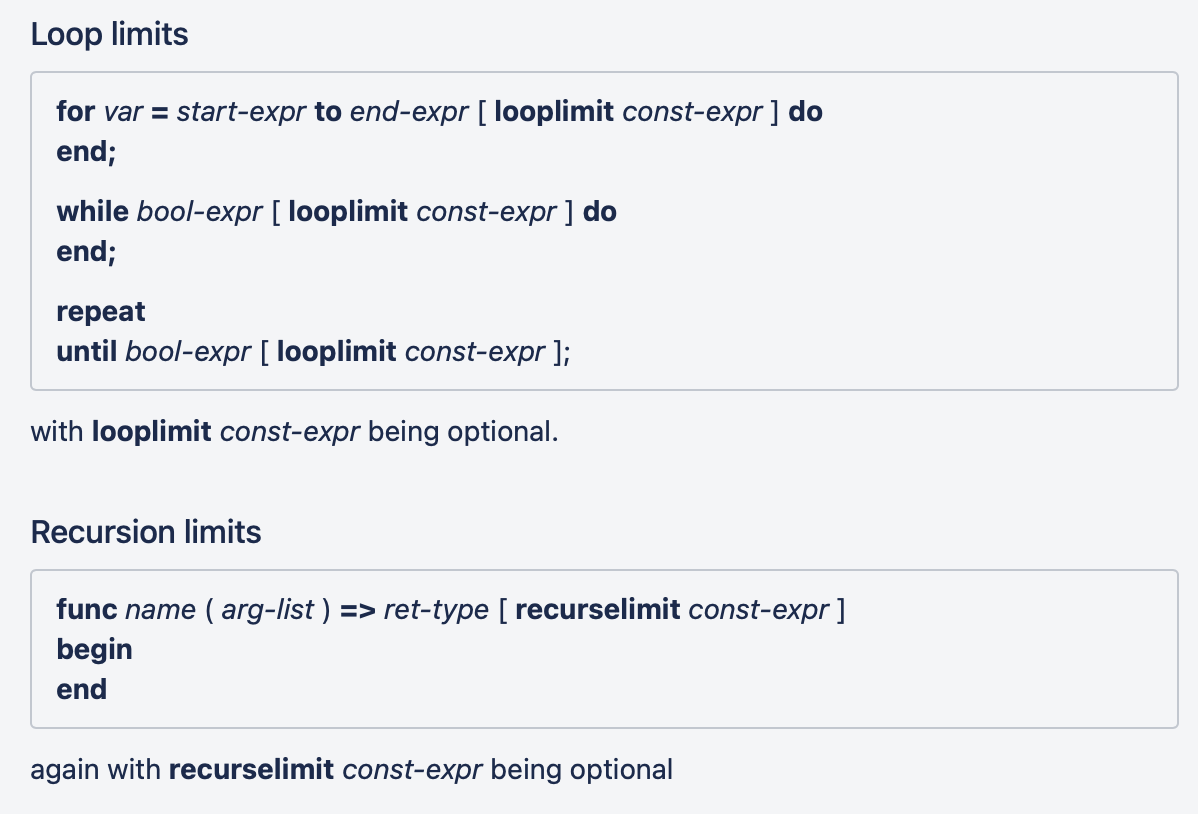
\includegraphics[width=\textwidth]{looprecurselimit.png}

\section{ASL-624: Base values}

The current base value rules apply so long as the type of the variable or
field is unconstrained or all of the constraint's expressions use only
compile-time constants and literals.

If the variable's or field's type are parameterized or the constraint
values cannot be determined statically, then it is the programmer's
responsibility to provide an explicit initialising assignment, since a
declaration should never have an undefined value. The initialising
expression does not need to be constant, but must satisfy the
constraints.

\section{ASL-629: Define side-effects}

The order of conflicting evaluations is explicitly defined in the ASLRef
specification. A summary is as follows.

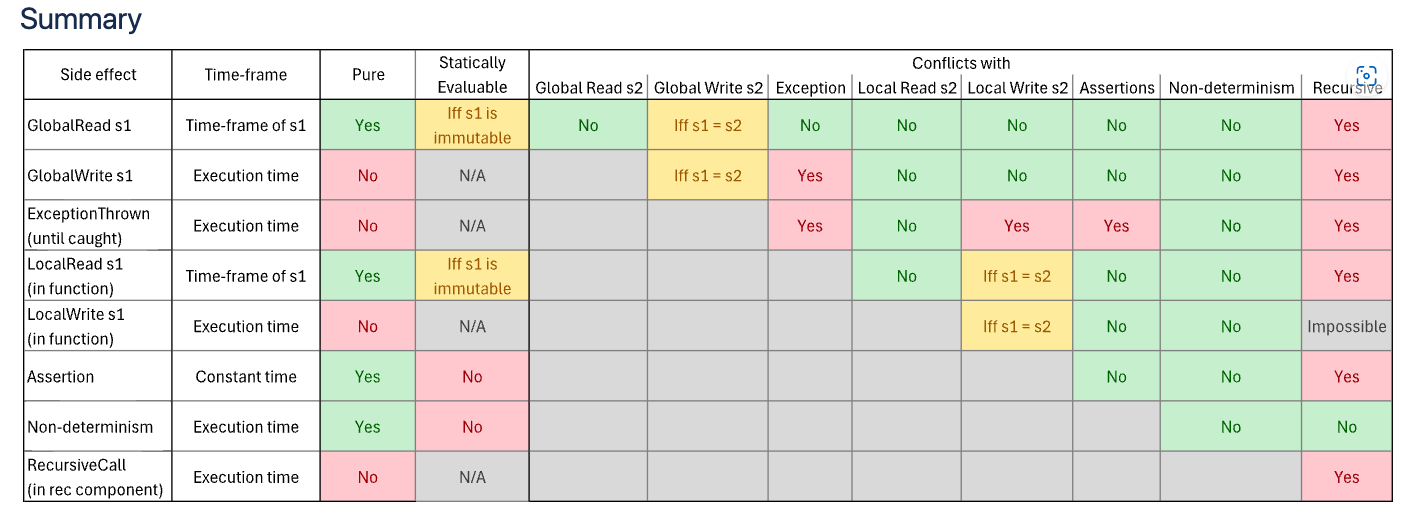
\includegraphics[width=\textwidth]{sideeffects.png}

\section{ASL-630: Behaviour of print}
There are two variants, \texttt{print} and \texttt{println}, which behave
as follows:
\begin{verbatim}
println("Hello world!");
println("Goodbye world!")
// Prints:
// Hello world!
// Goodbye world!
\end{verbatim}
whereas:
\begin{verbatim}
print("Hello world!");
println("Goodbye world!")
// Prints:
// Hello world!Goodbye world!
\end{verbatim}
In other words, \texttt{print} does not do any formatting such as adding any
newlines or spaces whereas \texttt{println} adds a single newline to the end of
the output.

A user can type in a series of prints to print a "concatenated" string as:
\begin{verbatim}
print("helloworld", 42); printMybitvector(mybits); println("");
\end{verbatim}

The following table summarises the supported values:\\
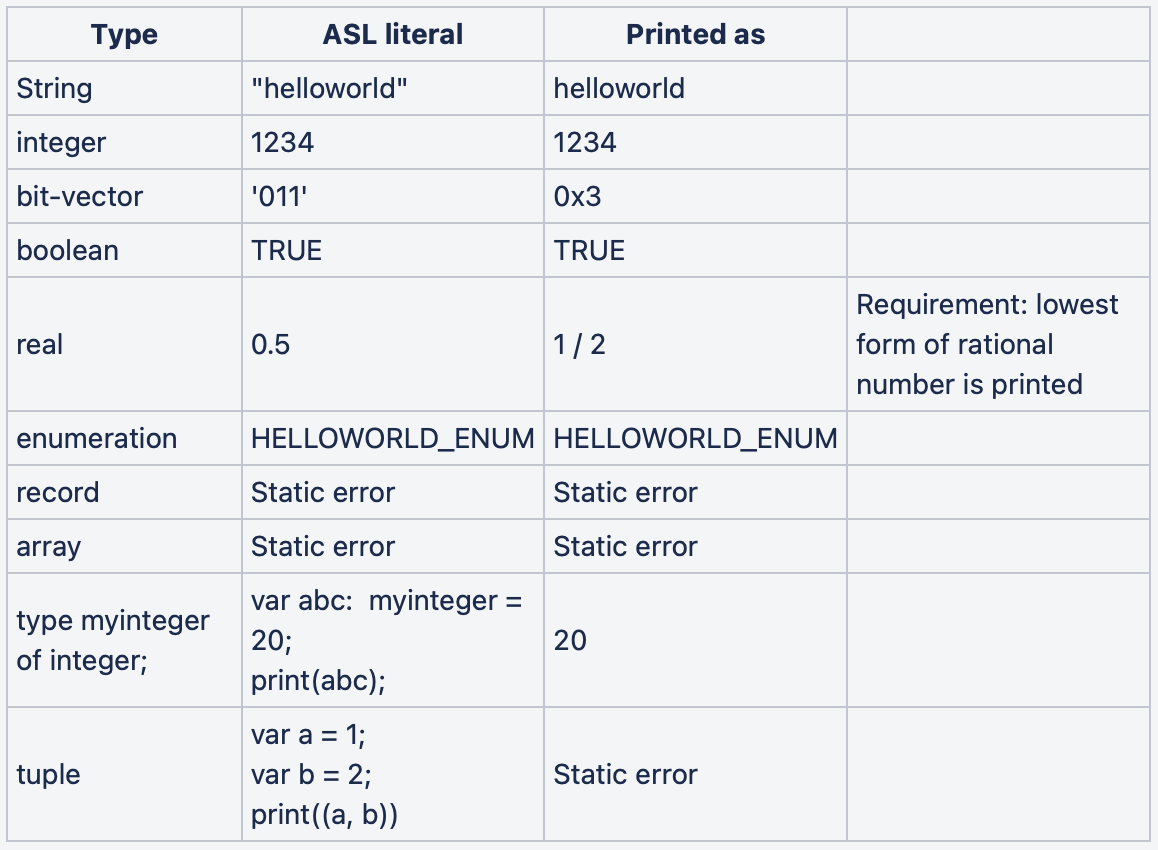
\includegraphics[width=\textwidth]{print.png}

\section{ASL-632: Parameters simplification}

\subsection{Functions must be declared with all parameters in braces}
None can be parameter-defining arguments.

\subsection{Parameters must be declared in a specific order}

Textually left-to-right as they appear in first the return type, then the
argument types.

\subsection{Functions must be called with all parameters instantiated using the braced syntax}
Except for the following (optional) cases:
\begin{itemize}
\item Standard library functions, which can omit their input parameters -
e.g. \texttt{UInt('111')}, \texttt{ZeroExtend\{64\}('111')}
\item Function calls immediately on right-hand sides of assignments where
the left-hand side is explicitly type annotated. These can inherit their
return parameter (first in the parameter list) from the left-hand side.
\end{itemize}

\subsection{Modify the signature of \texttt{Replicate} to align with \texttt{SignExtend} and \texttt{ZeroExtend}}

In other words, allow its parameters to be elided:
\begin{verbatim}
func Replicate{N,M}(x: bits(M)) => bits(N)
begin
  assert N MOD M == 0;
  ...
end
\end{verbatim}

\subsection{Call sites can elide empty argument lists \texttt{()} if
there is a non-empty parameter list}
For example, \texttt{Zeros\{64\}}. However, this cannot
be applied in conjunction with an elided single parameter on RHS.

\noindent
Examples:
\begin{verbatim}
// func Bar{N}(...) => bits(N)
// func Baz{A,B}(...) => bits(A)
let res : bits(N) = Bar{}(args);
  // omitted single parameter N (no ambiguity)
  // desugared to Bar{N}(args);
let res : bits(N) = Baz{,sz}(bv);
  // omitted positional parameter A
  // desugared to Baz{N,sz}(bv);
let res : bits(N) = Baz{}(bv);
  // ILLEGAL - only first parameter can be omitted

func{_}(..., x : bits(M), ..., y : bits(N)) => bits(L)
  // Parameters must be declared {L,M,N}

let res = Zeros{64};
  // can avoid empty argument list ()
let res : bits(64) = Zeros{}();
  // OK
let res : bits(64) = Zeros{64};
  // OK
let res : bits(64) = Zeros{};
  // INVALID - parsing conflict with empty record

let - = UInt('1111');
  // equivalent to UInt{4}('1111');
// func ZeroExtend{N,M}(x: bits(M)) => bits(N)
// no need to specify input parameter M
let - : bits(64) = ZeroExtend{64}('11');
  // equivalent to ZeroExtend{64,2}
let - : bits(64) = ZeroExtend{}('11');
  // can also elide the output parameter N
\end{verbatim}

\section{ASL-710: Syntax for \texttt{IN '10xx'}}

\subsection{Require that the \texttt{IN} set membership operator always
requires \{ and \} around the set}

This is regardless of the number of members.

In other words, forbid removal of \texttt{\{} and \texttt{\}} around a
single-member set---the following used to be permitted by ASL1 for
single-member sets but is not anymore:

\begin{itemize}
\item \texttt{Mybits IN \{'000x'\}} could be written as \texttt{Mybits IN '000x'}
\item \texttt{!Mybits IN \{'000x'\}} could be written as \texttt{!Mybits
IN '000x'}
\end{itemize}

\subsection{Reintroduce ASL0 syntactic sugar}

This means that:
\begin{itemize}
\item \texttt{Mybits IN \{'000x'\}} can be written as \texttt{Mybits == '000x'}
\item \texttt{!Mybits IN \{'000x'\}} can be written as \texttt{Mybits != '000x'}
\end{itemize}

\section{ASL-738: Rename \texttt{UNKNOWN} to \texttt{ARBITRARY}}

\texttt{UNKNOWN} keyword is renamed to \texttt{ARBITRARY}.


\section{ASL-637: Dynamic and static errors}

The taxonomy of ASL errors as dynamic or static has been captured in the ASLRef
specification. A summary is as follows.

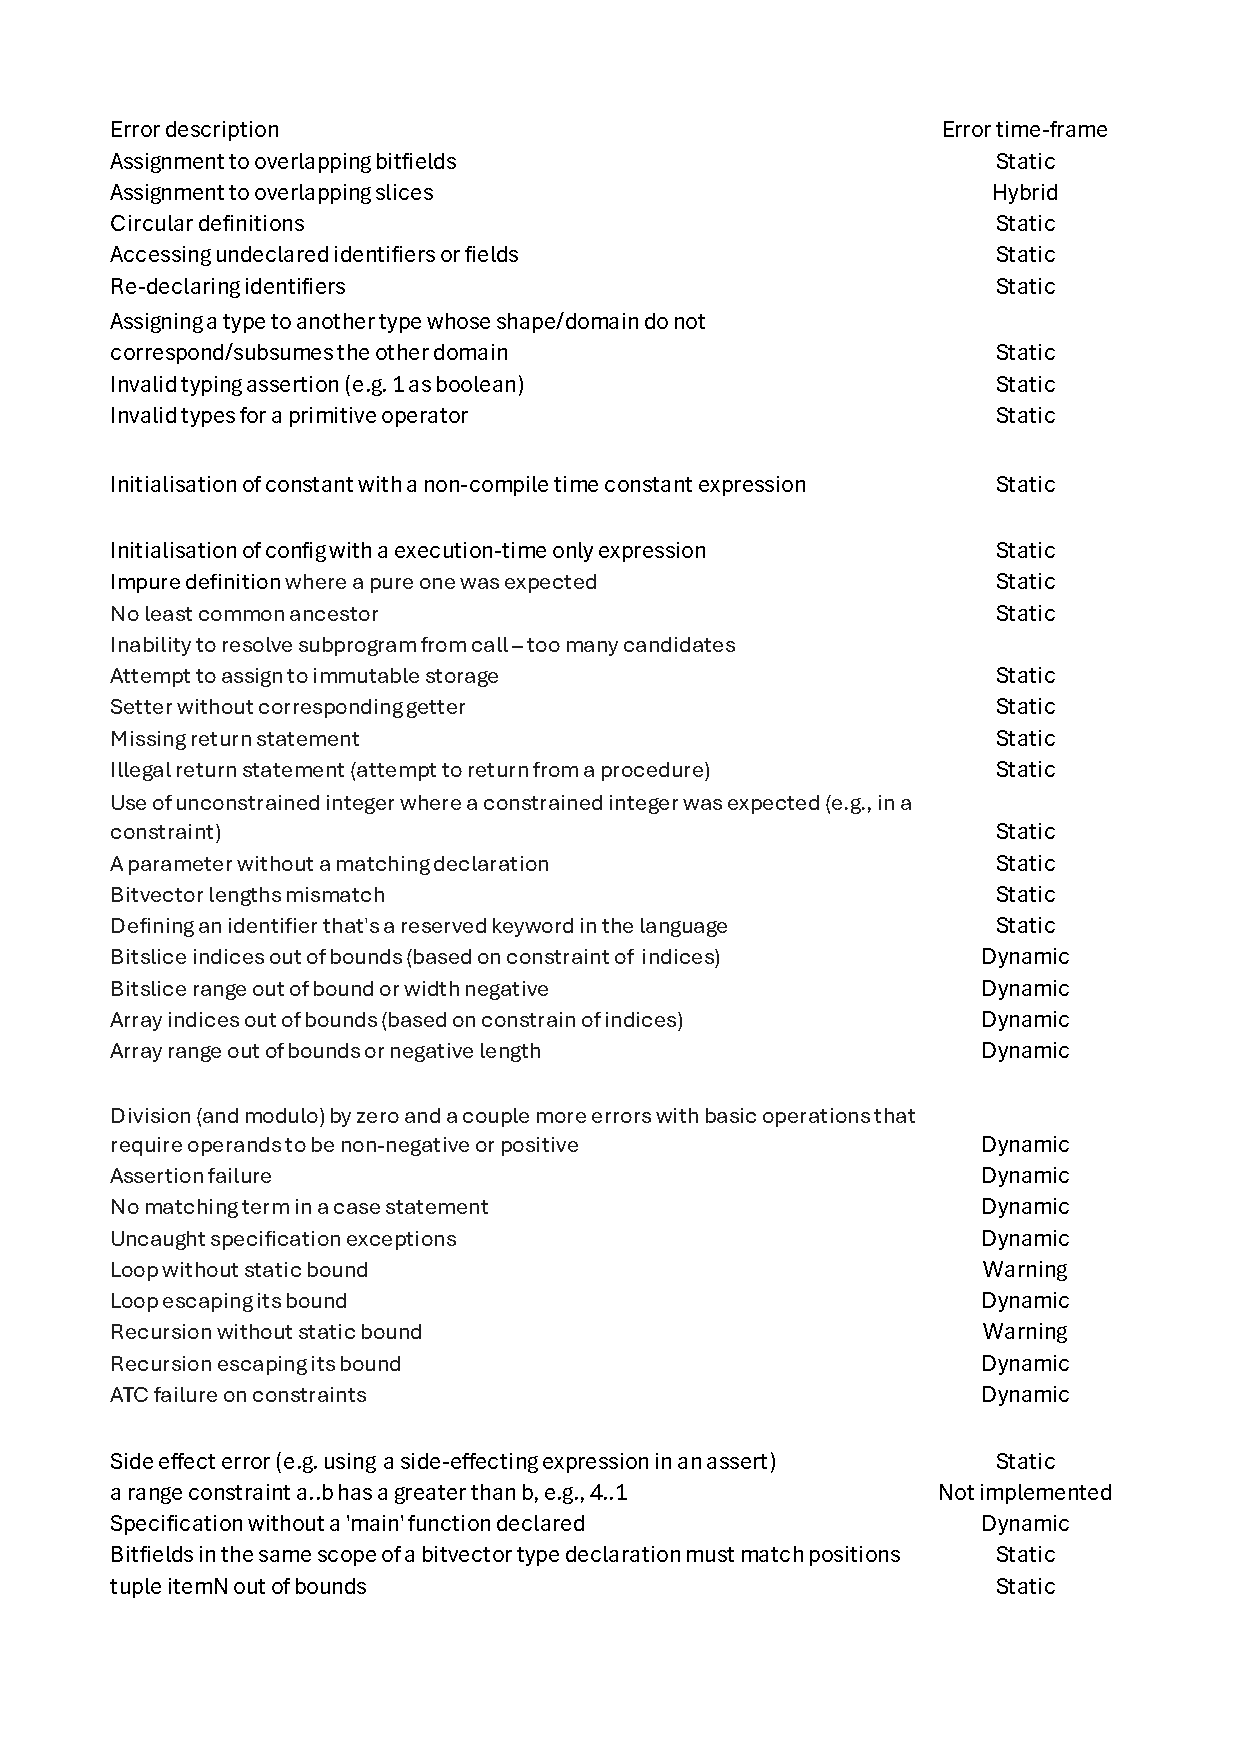
\includegraphics[width=\textwidth]{ASL-error-status.pdf}

\section{ASL-702: Underscore identifiers}

Any identifier with a double-underscore (\texttt{\_\_}) prefix is
treated as a static error by ASLRef. Other compilers might recognise
these identifiers as keywords for compiler-specific extensions.

Any identifier with a single underscore followed by an alphanumeric
character is treated as a normal identifier, but ASLRef recommends that
these are only for use by platform-specific code which should not clash
with the rest of a portable ASL program.

The following keywords are removed from the ASL reserved list:
\begin{verbatim}
access
advice
after
aspect
before
entry
expression
get
is
pattern
pointcut
replace
set
statements
watch
\end{verbatim}

\section{ASL-741: Behaviour of \texttt{ARBITRARY}}

Clarify behaviour of \texttt{ARBITRARY} as follows:

Each evaluation can produce a different arbitrary value, but (as always)
once a particular expression is evaluated, its arbitrary value cannot
change. This is because evaluation produces native values, and
\texttt{ARBITRARY} is not a valid native value - so once evaluated, it
becomes an unchanging native value like any other.  Note that there are
two important consequences of producing an arbitrary value when
evaluating expressions of the form \texttt{ARBITRARY : type}:
\begin{enumerate}
\item The arbitrary value depends only on type, and no other ASL storage
elements.

\item The only guarantee of the resulting value is that it is a valid member of
type. In particular, the language does not define which valid member it
is, and ASL specifications must not rely on the value (for example, there
is no way to test whether a value was produced by evaluating
\texttt{ARBITRARY}).
\end{enumerate}

\section{ASL-706: Getters and setters simplification}

\subsection{Forbid getters and setters without an argument list}

Although that list could be empty.

\subsection{Restrict setter usage on some left-hand sides}

For example, no setters in tuples.

\section{ASL-744: Clarifying left-hand sides}

\subsection{Mutable assignments}

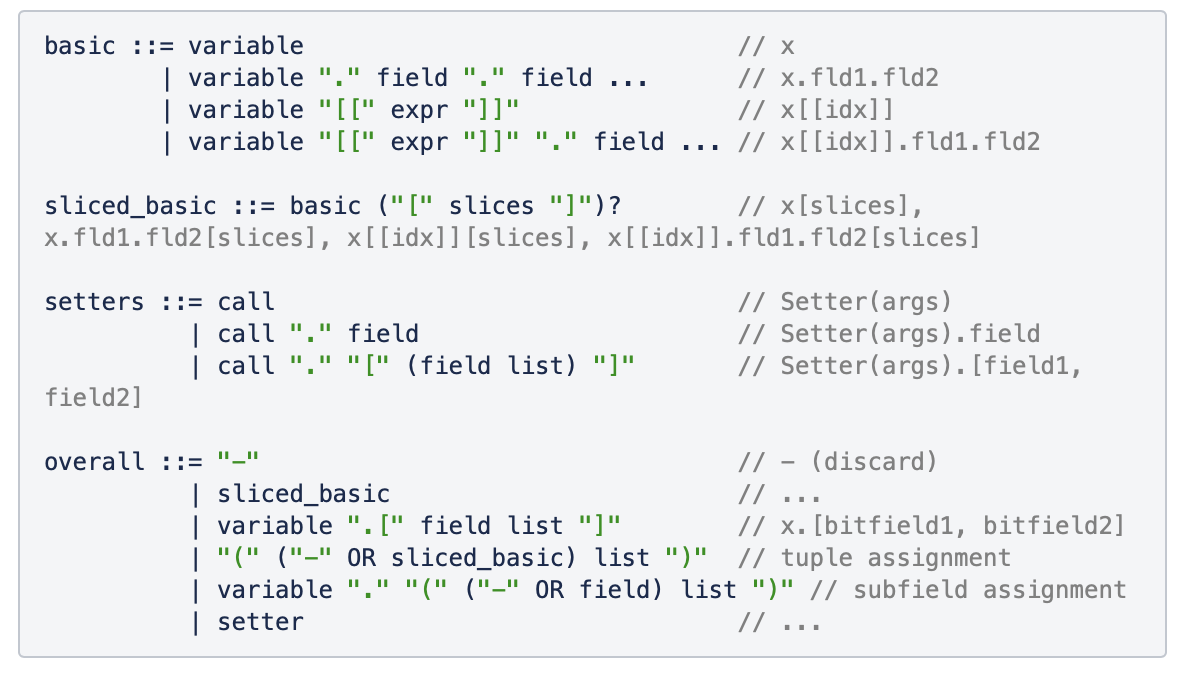
\includegraphics[width=\textwidth]{lhs-multiple.png}

\subsection{Declarations}

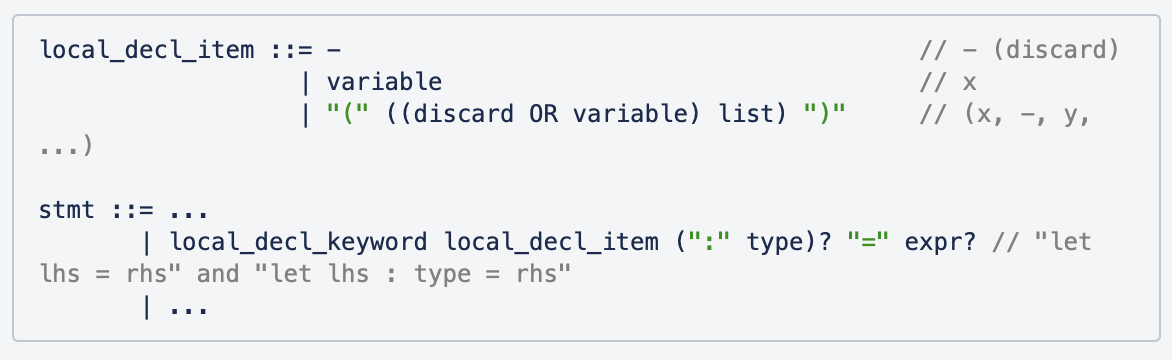
\includegraphics[width=\textwidth]{lhs-declarations.png}

\section{ASL-596: Remove \texttt{Int()} and \texttt{IsZeroBit()} in the standard library}

\section{ASL-539: Nested bitfields}

\subsection{Ensure that nested bitfields checks in ASLRef handle the following patterns}

\begin{verbatim}
type Nested_Type of bits(32) {
    [31:16] fmt0 {
        [15] : fixed,
        [14] : moving
    },
    [31:16] fmt1 {
        [15] : fixed,
        [0]  : moving
    },
    [31] : fixed,
    [0]  : fmt
};

var nested : Nested_Type;

// select the correct view of moving
// nested.fmt is '0'
//    nested.fmt0.moving is nested[30]
// nested.fmt is '1'
//    nested.fmt1.moving is nested[16]
let moving = if nested.fmt == '0' then
               nested.fmt0.moving
             else
               nested.fmt1.moving;

// below are all equivalent
let fixed = nested[31];
let fixed = nested.fixed;
let fixed = nested.fmt0.fixed;
let fixed = nested.fmt1.fixed;
\end{verbatim}

\subsection{Require that fields with same name occupy the same absolute bit
positions in all ancestor fields}

This will result in a static error if this requirement is not met.
\chapter{Introduction\label{chap:Introduction}}

This reference defines Arm’s Architecture Specification Language (ASL), which is the language
used in Arm’s architecture reference manuals to describe the Arm architecture.

ASL is designed and used to specify architectures. As a specification language, it is designed to be accessible,
understandable, and unambiguous to programmers, hardware
engineers, and hardware verification engineers, who collectively have quite a small intersection of languages they
all understand. It can intentionally under specify behaviors in the architecture being described.

ASL is:
\begin{itemize}
    \item a first-order language with strong static type-checking.
    \item whitespace-insensitive.
    \item imperative.
\end{itemize}

ASL has support for:
\begin{itemize}
    \item bitvectors:
    \begin{itemize}
        \item as a type.
        \item as a literal constant.
        \item bitvector concatenation.
        \item bitvector constants with wildcards.
        \item bitslices.
        \item dependent types to support function overloading using bitvector lengths.
        \item dependent types to reason about lengths of bitvectors.
    \end{itemize}
    \item unbounded arithmetic types “integer” and “real”.
    \item exceptions.
    \item enumerations.
    \item arrays.
    \item records.
    \item call-by-value.
    \item type inference.
\end{itemize}

ASL does not have support for:
\begin{itemize}
    \item references or pointers.
    \item macros.
    \item templates.
    \item virtual functions.
\end{itemize}

A \emph{specification} consists of a self-contained collection of ASL code.
\lrmcomment{\identd{GVBK}}
More specifically, a specification is the set of declarations written in ASL code which describe an architecture.

\section{Example Specification 1}
\listingref{spec1} shows a small example of a specification written in ASL. It consists of the following declarations:
\begin{itemize}
    \item Global bitvectors \texttt{R0}, \texttt{R1}, and \texttt{R2} representing the state of the system.
    \item A function \texttt{MyOR} demonstrating a simple bit-wise OR function of 2 bitvectors.
    \item Initialization of \texttt{R0} and \texttt{R1} bitvectors.
    \item Assignment of bitvector \texttt{R2} with the result of a function call.
\end{itemize}

\begin{center}
\lstinputlisting[caption=Example specification 1\label{listing:spec1}]{\definitiontests/spec1.asl}
\end{center}

\section{Example Specification 2}
\listingref{spec2} shows a small example of a specification written in ASL. It consists of the following declarations:
\begin{itemize}
\item A global variable \texttt{COUNT} representing the state of the system.
\item A procedure \texttt{ColdReset} to initialize the state of the system when power is applied and the system is reset.
    This interpretation of the function is a convention used in this particular specification. It is up to each
    specification to decide the role of each function.
\item A procedure \texttt{Step} to advance the state of the system. That is, it defines the \emph{transition relation} of the system.
    Again, this interpretation is a convention used in this particular specification, not part of the ASL language
    itself.
\end{itemize}

\begin{center}
\lstinputlisting[caption=Example specification 2\label{listing:spec2}]{\definitiontests/spec2.asl}
\end{center}

\section{Example Specification 3}
\listingref{spec3} shows a small example of a specification in ASL. It consists of the following declarations:
\begin{itemize}
    \item A function \texttt{Dot8} which operates on 2 bitvectors a byte at a time.
    \item A global variable \texttt{COUNT} to indicate the number of calls to the \texttt{Fib} function.
    \item A function \texttt{Fib} demonstrating recursion with a bound of 1000 on its depth.
    \item Assignment of a global bitvector \texttt{X} with a call to the \texttt{Dot8} function.
    \item Assignment of a variable from the result of a call to the recursive function \texttt{Fib}.
    \item A function \texttt{main}.
\end{itemize}

\ASLListing{Example specification 3}{spec3}{\definitiontests/spec3.asl}

\paragraph{Structure of this Reference:}
The rest of this document introduces elements of the ASL language and formalizes
them. First, the mathematical background needed to understand the formalization
is introduced in \chapref{FormalSystem}.
Then, we define the ASL lexical structure \chapref{LexicalStructure}, syntax \chapref{Syntax},
and ASL abstract syntax (AST) \chapref{AbstractSyntax}.
Familiarity with the AST is \underline{essential} for understanding the
type system (static semantics) and the dynamic semantics.
\chapref{TypeChecking}, and \chapref{Semantics} introduce the
definitions used to formalize the type system and dynamic semantics.
Following these chapters, the reference roughly follows the structure of the AST
in a bottom-up fashion, until reaching \chapref{TopLevel} where all of the formalisms
are used together to demonstrate how they can be utilized to form an interpreter
for an ASL specification.

\chapter{Formal System \label{chap:FormalSystem}}

In this part, we define the mathematical concepts and notations used throughout.
We start by defining general mathematical concepts
and then describe how sets of rules formally define functions and relations.

\section{Mathematical Definitions and Notations}

\hypertarget{def-triangleq}{}
We use $\triangleq$ to define mathematical concepts.

We define the following sets:
\begin{itemize}
\item \hypertarget{def-N}{
    $\N$ is the set of natural numbers, including $0$.
}

\item \hypertarget{def-Npos}{
    $\Npos$ is the set of natural numbers, excluding $0$.
}

\item
\hypertarget{def-Z}{
    $\Z$ is the set of integers.
}

\item
\hypertarget{def-Q}{
    $\Q$ is the set of rationals.
}

\hypertarget{def-bool}{}
\hypertarget{def-false}{}
\hypertarget{def-true}{}
\item $\Bool$ is the set of ASL Boolean literals, which consists of $\True$ and $\False$.
We employ these literals to represent the corresponding mathematical truth values,
which are used to denote whether logical assertions hold or not.
\hypertarget{def-land}{}
\hypertarget{def-lor}{}
We also employ the mathematical meaning of logical conjunction $\land$, logical disjunction $\lor$,
and logical negation $\neg$, given next.
For a set of Boolean values $A$:
\[
  \begin{array}{rcl}
  \land A &\triangleq&
  \begin{cases}
    \True & \text{if all values in A are }\True\\
    \False & \text{otherwise}
  \end{cases}\\
  \lor A &\triangleq&
  \begin{cases}
    \False & \text{if all values in A are }\False\\
    \True & \text{otherwise}
  \end{cases}\\
\end{array}
\]
\hypertarget{def-neg}{}
For a pair of Boolean values $a,b\in\Bool$, we define $a \land b \triangleq \land\{a, b\}$
and $a \lor b \triangleq \lor\{a, b\}$.
Finally, $\neg\True\triangleq\False$ and $\neg\False\triangleq\True$.

\item
\hypertarget{def-identifier}{}
    $\Identifiers$ is the set of all ASL identifiers.

\item
\hypertarget{def-astlabels}{}
    $\astlabels$ is the set of all labels of Abstract Syntax Tree (AST) nodes.

\item
\hypertarget{def-strings}{}
    $\Strings$ is the set of all ASCII strings.
\end{itemize}

We utilize the notation $\overname{a}{b}$ to enable us to name the mathematical term $a$ as $b$ so that
we can refer to it in text. We especially use this to name the input arguments and
output results of functions and relations. For example, the input argument of $\sign$,
which is defined next is named $q$.

\hypertarget{def-sign}{}
\begin{definition}[Sign of a Rational Number]
  The function $\sign : \overname{\Q}{q} \rightarrow \{-1,0,1\}$ returns the sign of $\vq$:
\[
\sign(q) \triangleq \begin{cases}
  1 & \text{if }q > 0\\
  0 & \text{if }q = 0\\
  -1 & \text{if }q < 0
\end{cases}
\]
\end{definition}

\begin{definition}[Empty Set]
  The \emph{empty set} --- the set that does not contain any element --- is denoted as $\emptyset$.
\end{definition}

\hypertarget{def-cardinality}{}
\begin{definition}[Set Cardinality]
  For a set $S$, the notation $\cardinality{S}$ stands for the number of elements in $S$.
\end{definition}

\hypertarget{def-pow}{}
\begin{definition}[Powerset]
  The \emph{powerset} of a set $A$, denoted as $\pow{A}$, is the set of all subsets of $A$, including the empty set and $A$ itself:
  \[
     \pow{A} \triangleq \{ B \;|\; B \subseteq A\} \enspace.
  \]
\end{definition}

\hypertarget{def-powfin}{}
\begin{definition}[Powerset of Finite Subsets]
  The \emph{powerset of finite subsets} of a set $A$, denoted as $\powfin{A}$, is the set of all finite subsets (including the empty set) of $A$:
  \[
     \powfin{A} \triangleq \{ B \;|\; B \subseteq A, |B| \in \N\} \enspace.
  \]
\end{definition}

\hypertarget{def-cartimes}{}
\begin{definition}[Cartesian Product]
    The \emph{Cartesian product} of sets $A$ and $B$, denoted $A \cartimes B$
    is $A \cartimes B \triangleq \{(a,b) \;|\; a \in A, b \in B\}$.
\end{definition}

\hypertarget{def-partialfunc}{}
\hypertarget{def-dom}{}
\begin{definition}[Partial Function\label{def:PartialFunction}]
  A \emph{partial function}, denoted $f : A \partialto B$, is a function from a \underline{subset} of $A$ to $B$.
  The \emph{domain} of a partial function $f$, denoted $\dom(f)$, is the subset of $A$ for which it is defined.
  We write $f(x) = \bot$ to denote that $x$ is not in the domain of $f$, that is, $x \not\in \dom(f)$.
\end{definition}

Notice that the domain of a partial function need not be finite, which is what the following definition covers.

\hypertarget{def-finfunction}{}
\begin{definition}[Finite-domain Function]
The notation $\rightarrowfin$ stands for a function \\ whose domain is finite.
\end{definition}

\hypertarget{def-emptyfunc}{}
\begin{definition}[Empty Function\label{def:EmptyFunction}]
The function with an empty domain is denoted as $\emptyfunc$.
\end{definition}

\begin{definition}[Function Update\label{def:FunctionUpdate}]
  The function denoted as $f[x \mapsto v]$ is a function identical to $f$, except that $x$ is bound
  to $v$. That is, if  $g = f[x \mapsto v]$ then
  \[
    g(z) =
  \begin{cases}
    v     & \text{if } z = x\\
    f(z)  & \text{otherwise } \enspace.
  \end{cases}
  \]

  The notation $\{i=1..k: a_i\mapsto b_i\}$ stands for the function formed from the corresponding input-output pairs:
  $\emptyfunc[a_1\mapsto b_1]\ldots[a_k\mapsto b_k]$.
\end{definition}

\begin{definition}[Function Restriction]
\hypertarget{def-restrictfunc}{}
The \emph{restriction} of a function $f : X \rightarrow Y$ to a subset of its domain
$A \subseteq \dom(f)$, denoted as $\restrictfunc{f}{A}$, is defined
in terms of the set of input-output pairs:
\[
  \restrictfunc{f}{A} \triangleq \{ (x, f(x)) \;|\; x \in A \} \enspace.
\]
\end{definition}

\begin{definition}[Function Graph]
\hypertarget{def-funcgraph}{}
The \emph{graph} of a finite-domain function $f : X \rightarrowfin Y$
is the list of input-output pairs for $f$, given in any order:
\[
\funcgraph(f) \triangleq \{ (x, f(x)) \;|\; x \in \dom(f) \} \enspace.
\]
\end{definition}

Throughout this document, we will annotate arguments of relations and functions, wherever it is useful,
by writing a name or an expression above the corresponding argument type.
This makes convenient to refer to arguments by referring to the corresponding names and helps identify
the expressions corresponding to the arguments.
For example,
\[
    \textsf{choice} : \overname{\Bool}{b} \cartimes \overname{T}{x} \cartimes \overname{T}{y} \rightarrow \overname{T}{z}
\]
defines a function type and lets us refer to the first argument as $b$, the second argument as $x$,
the third argument as $y$, and to the result as $z$.

A \emph{parametric function} is a function whose domain is not a priori fixed but rather
parameterized by the type of its arguments. An example is the $\textsf{choice}$ function where the type $T$ of
$x$, $y$, and $z$ is unspecified and inferred from the context where the function is used.

\hypertarget{def-choice}{}
\begin{definition}[Choice]
The parametric function $\textsf{choice} : \overname{\Bool}{b} \cartimes \overname{T}{x} \cartimes \overname{T}{y} \rightarrow \overname{T}{z}$,
is defined as follows:
\[
  \choice{\vb}{x}{y} \triangleq
  \begin{cases}
    x & \text{ if }\vb \text{ is }\True\\
    y & \text{ otherwise}\\
  \end{cases}
\]
\end{definition}

\subsection{Lists}
In the remainder of this document, we use the term \emph{list} and \emph{sequence} interchangeably.

A list of elements \hypertarget{def-emptylist}{is either empty, denoted by $\emptylist$}, or non-empty.
A non-empty list is either denoted by listing the elements in sequence, $v_1 \ldots\ v_k$,
or in bracketed form, $[v_1,\ldots,v_k]$, which is used to aesthetically separate it from surrounding mathematical expressions.
The commas carry no special meaning.

\hypertarget{def-head}{}
\hypertarget{def-tail}{}
For a non-empty list $v_1 \ldots\ v_k$, the \emph{\head} of the list is the first element --- $v_1$ ---
and the \emph{\tail} of the list is the suffix obtained by removing $v_1$ from the list.

We refer to individual elements of a non-empty list $V$ by the index notation $V[i]$ where $i\in\Npos$.

\hypertarget{def-listlen}{}
\begin{definition}[List Length]
The \emph{length} of a list is the number of elements in that list:
$\listlen{\emptylist} \triangleq 0$ and $\listlen{v_1,\ldots,v_k}=k$.
\end{definition}

We use the notation $a..b$, where $a,b\in\Z$ and as a shorthand for the interval $[a\ldots b]$
(counting up when $a \leq b$ and counting down when $a \geq b$).
We write $x_{a..b}$ as a shorthand for the sequence $x_a \ldots x_b$.
%
We write $i=1..k: V(i)$, where $V(i)$ is a mathematical expression parameterized by $i$,
to denote the sequence of expressions $V(1) \ldots V(k)$.
The notation $a \in A: V(a)$, where $A$ is a set and $V$ is an expression parameterized by the free variable $a$,
stands for $V(a_1) \ldots V(a_k)$ where $a_{1..k}$ is an arbitrary ordering of the elements of $A$.

We write $T^*$ to denote a the type of a possibly-empty list of elements of type $T$,
and $T^+$ for a non-empty list of elements of type $T$.

\hypertarget{def-listset}{}
\begin{definition}[Listing a Set]
The parametric relation $\listset : \pow{T} \times T^*$
lists the elements of a set in an arbitrary order:
\[
\begin{array}{c}
  \listset(X) = x_{1..k}\\
  |X| = k\\
  \forall x\in X.\ \exists 1 \leq i \leq k.\ x = x_i
\end{array}
\]
\end{definition}

\hypertarget{def-concat}{}
\begin{definition}[List Concatenation]
The parametric function $\concat : T^* \cartimes T^* \rightarrow T^*$ concatenates two lists:
\[
    \begin{array}{rcl}
    \emptylist \concat L &\triangleq& L\\
    L \concat \emptylist &\triangleq& L\\
    l_{1..k} \concat m_{1..n} &\triangleq& [l_{1..k}, m_{1..n}]
    \end{array}
\]
\end{definition}

\hypertarget{def-equallength}{}
\begin{definition}[Equating List Lengths]
The parametric function
\[
  \equallength : \overname{L}{a} \cartimes \overname{L}{b} \rightarrow \Bool
\]
compares the length of two lists:
\[
\equallength(a, b) \triangleq \listlen{a}=\listlen{b} \enspace.
\]
\end{definition}

\hypertarget{def-listprefix}{}
\begin{definition}[List Prefix]
The parametric function $\listprefix : \overname{T^*}{\vlone} \cartimes \overname{T^*}{\vltwo} \rightarrow \Bool$ checks whether
the list $\vlone$ is a \emph{prefix} of the list $\vltwo$:
\[
\listprefix(\vlone, \vltwo) \triangleq \exists \vlthree.\ \vltwo = \vlone \concat \vlthree \enspace.
\]
\end{definition}

\hypertarget{def-listrange}{}
\begin{definition}[Indices of a List]
The parametric function $\listrange : T^* \rightarrow \N^*$ returns the ($1$-based) list of indices for a given list:
\[
    \begin{array}{rcl}
        \listrange(\emptylist) &\triangleq& \emptylist\\
        \listrange(v_{1..k}) &\triangleq& [1..k] \enspace.
    \end{array}
\]
\end{definition}

% \hypertarget{def-filterlist}{}
% \begin{definition}[Filtering a List]
% The parametric function
% \[
% \filterlist : \overname{T^*}{l} \times \overname{(T \rightarrow \Bool)}{p} \rightarrow T^*
% \]
% retains the elements of the list $l$ for which the predicate $p$ returns $\True$:
% \[
% \begin{array}{rcl}
% \filterlist(\emptylist, p) &\triangleq& \emptylist\\
% \filterlist([h] \concat t, p) &\triangleq& \begin{cases}
% [h]\concat \filterlist(t) & \text{if }p(h) = \True\\
%  \filterlist(t) & \text{else}\\
% \end{cases}\\
% \end{array}
% \]
% \end{definition}

\hypertarget{def-unziplist}{}
\begin{definition}[Unzipping a List of Pairs]
The parametric function
\[
\unziplist : (T_1 \cartimes T_2)^* \rightarrow (T_1^* \cartimes T_2^*)
\]
transforms a list of pairs into the corresponding pair of lists:
\[
  \unziplist(\pairs) \triangleq \begin{cases}
    (\emptylist, \emptylist)  & \text{if }\pairs = \emptylist\\
    (a_{1..k}, b_{1..k})      & \text{else }\pairs = (a_1,b_1) \ldots (a_k,b_k)  \enspace.
  \end{cases}
\]
\end{definition}

\hypertarget{def-unziplistthree}{}
\begin{definition}[Unzipping a List of Triples]
The parametric function
\[
\unziplistthree : (T_1 \cartimes T_2 \cartimes T_3)^* \rightarrow (T_1^* \cartimes T_2^* \cartimes T_3^*)
\]
transforms a list of triples into the corresponding triple of lists:
\[
  \unziplistthree(\triples) \triangleq \begin{cases}
    (\emptylist, \emptylist, \emptylist)  & \text{if }\triples = \emptylist\\
    (a_{1..k}, b_{1..k}, c_{1..k})      & \text{else }\triples = (a_1,b_1,c_1) \ldots (a_k,b_k,c_k)  \enspace.
  \end{cases}
\]
\end{definition}

\hypertarget{def-uniquelist}{}
\hypertarget{def-uniquep}{}
\begin{definition}[Finding unique elements of a list]
The parametric function
\[
\uniquelist : \overname{T^*}{l} \rightarrow T^*
\]
retains only the first occurrence of each element of the list $l$.
It relies on the helper function $\uniquep$:
\[
\begin{array}{rcl}
\uniquelist(l) &\triangleq& \uniquep(l, \emptylist)\\\\
\uniquep(\emptylist, \acc) &\triangleq& \acc\\
\uniquep([h] \concat t, \acc) &\triangleq&
  \begin{cases}
    \uniquep(t, \acc) & \text{if }h \in t\\
    \uniquep(t, \acc \concat [h]) & \text{otherwise}\\
  \end{cases}
\end{array}
\]
\end{definition}

\subsection{Strings}
\hypertarget{def-stringconcat}{}
The function $\stringconcat : \Strings \times \Strings \rightarrow \Strings$
concatenates two strings.

\hypertarget{def-stringofnat}{}
The function $\stringofnat : \N \rightarrow \Strings$ converts a natural number
to the corresponding string.

\subsection{OCaml-style Notations}
We use the following notations, which are in the style of the OCaml programming language,
to facilitate correspondence with our
\href{https://github.com/herd/herdtools7/tree/master/asllib}{reference implementation}.

The notation $L(v_{1..k})$ is a compound term where $L$ is a label and $v_{1..k}$ is a (possibly singleton) list of mathematical values.
We also write $L(T_{1..k})$, where $T_{1..k}$ denotes mathematical types of values, to stand for the type
$\{ L(v_{1..k}) \;|\; v_1\in T_1,\ldots,v_k\in T_k \}$.

\hypertarget{def-optional}{}
\begin{definition}[Optional]
\hypertarget{def-none}{}
\hypertarget{def-some}
The notation $\Some{\cdot}$ stands for either an empty set or a singleton set,
where $\None\triangleq\langle\rangle$ denotes an empty set
and $\Some{v}$ denotes a set containing the single element $v$.
%
The notation $\Some{T}$, where $T$ denotes a mathematical type, stands for
$\{ \None \} \cup \{\Some{v} \;|\; v \in T\}$.
%
We refer to $\Some{T}$ as an \emph{\optional}.
\end{definition}

%%%%%%%%%%%%%%%%%%%%%%%%%%%%%%%%%%%%%%%%%%%%%%%%%%%%%%%%%%%%%%%%%%%%%%%%%%%%%%%%
\section{Inference Rules}
%%%%%%%%%%%%%%%%%%%%%%%%%%%%%%%%%%%%%%%%%%%%%%%%%%%%%%%%%%%%%%%%%%%%%%%%%%%%%%%%
\hypertarget{def-inferencerule}{}
An \emph{\inferencerule} (rule, for short) is an implication between a set of logical assertions,
called the \emph{premises} of the rule,
and a \emph{conclusion} assertion.
The conclusion holds when the \underline{conjunction} of its premises holds.

We use the following rule notation, where $P_{1..k}$ are the rule premises and $C$ is the conclusion:
\begin{mathpar}
  \inferrule{P_1 \and \ldots \and P_k}{C}
\end{mathpar}

For example, the rule \TypingRuleRef{ELit} has one premise:
\begin{mathpar}
\inferrule{
  \annotateliteral{\vv} \typearrow \vt
}{
  \annotateexpr{\tenv, \ELiteral(\vv)} \typearrow (\vt, \ELiteral(\vv))
}
\end{mathpar}

and the rule \TypingRuleRef{EBinop} (somewhat simplified here) has three premises:
\begin{mathpar}
\inferrule{
  \annotateexpr{\tenv, \veone} \typearrow (\vtone, \veone') \\\\
  \annotateexpr{\tenv, \vetwo} \typearrow (\vttwo, \vetwo') \\\\
  \applybinoptypes(\tenv, \op, \vtone, \vttwo) \typearrow \vt
}{
  \annotateexpr{\tenv, \EBinop(\op, \veone, \vetwo)} \typearrow (\vt, \EBinop(\op, \veone', \vetwo'))
}
\end{mathpar}

The free variables appearing in the premises and conclusion are interpreted \underline{universally}.
That is, the rules apply to any values (of the appropriate types) assigned to their free variables.
%
For example, the rule \TypingRuleRef{EBinop} applies to any choice of values for the free variables
$\tenv$ (a static environment),
$\veone$, $\vetwo$, $\veone'$, $\vetwo'$ (expressions),
$\vt$, $\vtone$, and $\vttwo$ (types).

\begin{definition}[Grounding]
Assertions can be \emph{grounded} by substituting their free variables with values.
A \emph{ground rule} is a rule with all its assertions (premises and conclusion) grounded.
\end{definition}
For example,
the following is a grounding of \TypingRuleRef{EBinop}
\begin{mathpar}
\inferrule{
  \annotateexpr{\emptytenv, \ELiteral(\lint(2))} \typearrow (\TInt, \ELiteral(\lint(2))) \\\\
  \annotateexpr{\emptytenv, \ELiteral(\lint(3))} \typearrow (\TInt, \ELiteral(\lint(3))) \\\\
  \applybinoptypes(\emptytenv, \MUL, \TInt, \TInt) \typearrow \TInt
}{
  \annotateexpr{\emptytenv, \EBinop(\MUL, \ELiteral(\lint(2)), \ELiteral(\lint(3)))} \typearrow \\ (\TInt, \EBinop(\MUL, \ELiteral(\lint(2)), \ELiteral(\lint(3))))
}
\end{mathpar}
obtained by the following substitutions:
\begin{tabular}{ll}
  \textbf{free variable} & \textbf{value}\\
  \hline
  $\tenv$   & $\emptytenv$\\
  $\veone$  & $\ELiteral(\lint(2))$\\
  $\veone'$  & $\ELiteral(\lint(2))$\\
  $\vetwo$  & $\ELiteral(\lint(3))$\\
  $\vetwo'$  & $\ELiteral(\lint(3))$\\
  $\vt$    & $\TInt$\\
  $\vtone$    & $\TInt$\\
  $\vttwo$    & $\TInt$\\
  $\op$       & $\MUL$
\end{tabular}

A set of rules is interpreted \underline{disjunctively}. That is, each rule is used to determine whether its conclusion
holds independently of other rules.

\begin{definition}[Axiom]
An \emph{axiom} is a rule with an empty set of premises.
An axiom is denoted by simply stating its conclusion.
\end{definition}

An example of an axiom in the ASL type system is \TypingRuleRef{SPass}:
\begin{mathpar}
\inferrule{}{\annotatestmt(\tenv, \SPass) \typearrow (\SPass,\tenv)}
\end{mathpar}
\hypertarget{SemanticsRule.PAll-example}{}
An example of an axiom in the ASL semantics is \SemanticsRuleRef{PAll}:
\begin{mathpar}
\inferrule{}{
  \evalpattern{\env, \Ignore, \PatternAll} \evalarrow \Normal(\nvbool(\True), \emptygraph)
}
\end{mathpar}

To show that a specification is correct, with respect to the set of type rules,
or to show that a specification evaluates to a certain value, with respect to
the set of semantic rules, we must apply rules to form a \emph{derivation tree}.

\hypertarget{def-derivationtree}{}
\begin{definition}[Derivation Tree]
  A \emph{derivation tree} is a tree whose vertices correspond to ground assertions.
  More specifically, the leaves of a derivation tree correspond to ground axioms,
  and an internal vertex corresponds to a ground conclusion of a rule with its children
  corresponding to the ground premises of the same rule.
\end{definition}

\subsection{Transitions\label{sec:transitions}}

We use rules as a structured way for defining relations (and therefore functions, as a special case).

To define a relation $R \subseteq X \cartimes Y$, we use assertions of the form $\termx \rulearrow \termy$
where $\termx$ and $\termy$ are logical terms denoting sets of elements from $X$ and $Y$, respectively.
%
We call such assertions \emph{transitions}.
A set of rules $M$ with transition assertions defines the relation
\[
    R = \{ (x,y) \;|\; x \rulearrow y \text{ can be derived from rules in } M\} \enspace.
\]

For example, the rule \TypingRuleRef{ELit} defines a relation
between the infinite set of elements of the form
$\annotateexpr{\tenv, \ELiteral(\vv)}$ (for the
infinite choice of values for the free variables $\tenv$ and
$\vv$) to the infinite set of pairs of the form $(\vt,
\ELiteral(\vv))$, such that the premise holds.

\paragraph{Mutual Exclusion Principle:}
Our rules follow (with very few deviations, which we point out
in context) a mutual exclusion principle, where each rule
defines a relation disjoint from the ones defined by the other
rules.  This makes it easy to determine the rule responsible
for a given transition.

\hypertarget{def-configuration}{}
\subsection{Configurations}

\hypertarget{def-configdomain}{}
Our relations range over compound values. That is, values that often nest tuples and lists inside other tuples and lists.
We refer to such values as \emph{configurations}. To make it easier to distinguish between different configurations,
we will sometimes attach labels to tuples using the OCaml-style notation discussed earlier.
We refer to those labels as \emph{configuration domains}.
The domain of a configuration $C=L(\ldots)$, denoted $\configdomain{C}$, is the label $L$.

We refer to configurations at the origin of a transition as \emph{input configurations} and to the
configurations at the destination of a transition as \emph{output transitions}.

For example, the conclusion of the rule \TypingRuleRef{ELit} has \\
$\annotateexpr{\tenv, \ELiteral(\vv)}$ as its input configuration
and $(\vt, \ELiteral(\vv))$ as its output configuration.
Further, \\
$\configdomain{\annotateexpr{\tenv, \ELiteral(\vv)}} = \textit{annotate\_expr}$,
while the output configuration does not have a configuration domain, since it is an unlabelled pair.

Our rules always make use of labelled input configurations. This makes it easier to ensure
the mutual exclusion rule principle.

Our rules always define relations whose sets of input configurations and output configurations are disjoint.

\hypertarget{def-freshvariables}{}
\begin{definition}[Fresh Element]
  Premises of the form \texttt{$x\in T$ is fresh} mean that in any
  instantiation in a derivation tree, the value of $x$ is unique.
  That is, different from all other values instantiated for any other variable.
\end{definition}

\hypertarget{def-ignore}{}
\begin{definition}[Ignore Variable]
To keep rules succinct, we write $\Ignore$ for a mathematical variable whose name is
irrelevant for understanding the rule, and can thus be omitted.
Each \underline{occurrence} of $\Ignore$ represents a variable whose name is
different from any other free variable in the rule.
\end{definition}

For example, the rule \SemanticsRuleRef{PAll}, shown \hyperlink{SemanticsRule.PAll-example}{above},
uses an ignore variable to stand for the value being matched by a \texttt{-} pattern.
Since the rule does not need to refer to the value, we do not name it and use an ignore variable
instead.

\subsection{Flavors of Equality In Rules \label{sec:FlavoursOfEqualityInRules}}
We now explain equality notations in rules, two of which are used in \SemanticsRuleRef{ECond},
shown here:
\begin{mathpar}
\inferrule{
  \evalexpr{\env, \econd} \evalarrow \Normal(\mcond, \envone) \OrAbnormal\\\\
  \mcond \eqname (\nvbool(\vb), \vgone)\\
  \vep \eqdef \choice{\vb}{\veone}{\vetwo}\\\\
  \evalexpr{\envone, \vep} \evalarrow \Normal((\vv, \vgtwo), \newenv)  \OrAbnormal\\\\
  \vg \eqdef \ordered{\vgone}{\aslctrl}{\vgtwo}
}{
  \evalexpr{\env, \overname{\ECond(\econd, \veone, \vetwo)}{\ve}} \evalarrow
  \Normal((\vv, \vg), \newenv)
}
\end{mathpar}

\begin{description}
  \item[Range:] we write $i=1..k$ to allow listing premises parameterized by $i$ or constructing
  lists from expressions parameterized by $i$.
  For example, given two lists $a$ and $b$,
  \[
    i=1..k: a[i] > b[i]
  \]
  is the list of premises
  \[
    \begin{array}{l}
    a[1] > b[1]\\
    \ldots\\
    a[k] > b[k] \enspace.
    \end{array}
  \]

  \item[Predicate:] we write $a = b$ as an assertion of the equality of $a$ and $b$.
  For example, the mathematical identity $x \times (y + z) = x \times y + x \times z$.

  \hypertarget{def-deconstruction}{}
  \item[Deconstruction / ``View as'':] some values, such as tuples, are compound. In order to refer to the structure
  of compound values, we write $v \eqname \textit{f}(u_{1..k})$ where the expression on the right
  hand side exposes the internal structure of $v$ by introducing the variables
  $u_{1..k}$, allowing us to alias internal components of $v$.
  Intuitively, $v$ is re-interpreted as $\textit{f}(u_{1..k})$.
  For example, suppose we know that $v$ is a pair of values.
  Then, $v \eqname (a, b)$ allows us to alias $a$ and $b$.
  In \SemanticsRuleRef{ECond}, we know from the definition of $\evalexpr$ that
  $\mcond$ is a pair datatype.
  Therefore, writing $\mcond \eqname (\nvbool(\vb), \vgone)$ allows us to name each component of this pair
  and then refer to it, while \hyperlink{def-ignore}{ignoring} the static environment component.
  Similarly, if $v$ is a non-empty list, then $v \eqname [h] + t$ deconstructs the list into the
  head of the list $h$ and its tail $t$.
  Given that a variable $v$ represents a list, we write $v \eqname v_{1..k}$ to list its elements and allow
  referring to them by index.

  \hypertarget{def-eqdef}{}
  \item[Definition / ``Define as'':] the notation $\vx \eqdef \ve$ denotes that $\vx$ is a new name serving as an alias for the expression $\ve$.
  For example, in the rule \SemanticsRuleRef{ECond}, we use $\vg$ to name the mathematical expression
  $\ordered{\vgone}{\aslctrl}{\vgtwo}$.
  Aliases allow us to break down complex expressions, but rules can always be rewritten without them,
  by inlining their right-hand sides:
\begin{mathpar}
\inferrule{
  \evalexpr{\env, \econd} \evalarrow \Normal(\mcond, \envone) \OrAbnormal\\\\
  \mcond \eqname (\nvbool(\vb), \vgone)\\
  \evalexpr{\envone, \choice{\vb}{\veone}{\vetwo}} \evalarrow \Normal((\vv, \vgtwo), \newenv) \OrAbnormal
}{
  \evalexpr{\env, \overname{\ECond(\econd, \veone, \vetwo)}{\ve}} \evalarrow
  \Normal((\vv, \ordered{\vgone}{\aslctrl}{\vgtwo}), \newenv)
}
\end{mathpar}
\end{description}

\subsection{AST-related Notations}

When deconstructing AST record nodes such as $\{f_1:t_1,\ldots,f_k:t_k\}$,
we sometimes only care about a subset of the fields $\{f_{i_1},\ldots,f_{i_m}\} \subset \{f_{1..k}\}$.
In such cases, we write $\{f_{i_1}:t_{i_1},\ldots,f_{i_m}:t_{i_m},\ldots\}$,
where $\ldots$ stands for fields that are irrelevant for the rule.

For example\footnote{This example is from \SemanticsRuleRef{FCall}.}, the \func\ non-terminal is of a record type and has the following fields:
$\textsf{name}$, $\textsf{parameters}$, $\textsf{args}$, $\textsf{body}$, $\textsf{return\_type}$, and $\textsf{subprogram\_type}$.
The notation $\{ \textsf{body}:\SBASL(\texttt{body}),\ \textsf{args}:\texttt{arg\_decls}, \ldots \}$
allows us to deconstruct a given \func\ node by matching only the \textsf{body} and \textsf{args} fields.

Recall that a subset of AST nodes are either labels or labelled tuples.
\hypertarget{def-astlabel}{}
The partial function $\astlabel$ returns the label $\vl\in\astlabels$ of an AST node, when it exists.
For example, $\astlabel(\TBool) = \TBool$ and $\astlabel(\TNamed(\texttt{x})) = \TNamed$.

\subsection{How to Parse Rules Efficiently}
Consider the following examples, which is a simplified version of \SemanticsRuleRef{Binop}
\begin{mathpar}
  \inferrule{\op \not\in \{\BAND, \BOR, \IMPL\}\\\\
    \evalexpr{ \env, \veone} \evalarrow \Normal(\vmone, \envone) \\\\
    \evalexpr{ \envone, \vetwo } \evalarrow \Normal(\vmtwo, \newenv) \\\\
    \vmone \eqname (\vvone, \vgone) \\
    \vmtwo \eqname (\vvtwo, \vgtwo) \\
    \binoprel(\op, \vvone, \vvtwo) \evalarrow \vv \\\\
    \vg \eqdef \vgone \parallelcomp \vgtwo
  }
  {
    \evalexpr{ \env, \EBinop(\op, \veone, \vetwo) } \evalarrow
    \Normal((\vv, \vg), \newenv)
  }
\end{mathpar}

To parse a rule, start by examining the conclusion and the variables appearing in the rule.
In this case, the rule describes a transition from an input configuration \\
$\evalexpr{ \env, \EBinop(\op, \veone, \vetwo) }$,
whose configuration domain is \texttt{eval\_expr}, to an output configuration $\Normal((\vv, \vg), \newenv)$
whose configuration domain is $\Normal$.
%
A rule uses the free variables appearing in the input configuration of the conclusion
($\env$, $\op$, $\veone$, and $\vetwo$ in our example),
with the goal of assigning values to the free variables in the output configuration
of the conclusion ($\vv$, $\vg$, and $\newenv$, in our example).

Now, scan the premises in order to see where $\env$, $\op$, $\veone$, and $\vetwo$ are used and how
premises assign values to $\vv$, $\vg$, and $\newenv$.
%
In this case, $\vv$ is assigned as the result of the transition assertion
$\binoprel(\op, \vvone, \vvtwo) \evalarrow \vv$,
$\vg$ is assigned the expression $\vgone \parallelcomp \vgtwo$,
and $\newenv$ is assigned as the result of the transition assertion
$\evalexpr{ \envone, \vetwo } \evalarrow \Normal(\vmtwo, \newenv)$.
%
Notice that to assign values to the variables $\vv$, $\vg$, and $\newenv$,
intermediate values have to be assigned first.
For example, $\evalexpr{ \env, \veone} \evalarrow \Normal(\vmone, \envone)$
assigned values to $\envone$, which is then used by the transition \\
$\evalexpr{ \envone, \vetwo } \evalarrow \Normal(\vmtwo, \newenv)$.
Similarly, $\vg$ requires first assigning values to $\vgone$ and $\vgtwo$,
which are components of the previously assigned variables $\vmone$ and $\vmtwo$.

\subsection{Short-Circuit Rule Macros}

\emph{Short-circuit rule macros}, or \emph{rule macros}, for short, allow us to succinctly define sets of rules.
Specifically, they allow us to capture situations where
transitions have two alternative output configurations.
If the transition results in the first of the alternative output configurations, the following premises are considered.
However, if the result is the second, short-circuit output configuration, then the following premises are ignored
and the conclusion transitions into the short-circuit output configuration.
These short-circuit output configurations are typically, but not always, due to (type or dynamic) errors.

\hypertarget{def-terminateas}{}
In the following, $\XP$ and $\XQ$ stand for, possibly empty, sequences of premises.
%
A rule macro includes the special premise form $C \rulearrow C' \terminateas E$,
which introduces alternative output configurations $C'$ and short-circuit $E$:
\begin{mathpar}
  \inferrule{
    \XP\\\\
    C \rulearrow C' \terminateas E\\\\
    \XQ\\
  }
  {
    V \rulearrow V'
  }
\end{mathpar}
Such a rule macro expands to the following pair of rules:
\begin{mathpar}
  \inferrule[(Option 1)]{
    \XP\\\\
    C \rulearrow C' \\\\
    \XQ\\
  }
  {
    V \rulearrow V'
  }
  \and
  \inferrule[(Option 2:Short-circuited)]{
    \XP\\\\
    C \rulearrow E
  }
  {
    V \rulearrow E
  }
\end{mathpar}
Intuitively, if $C$ transitions to $C'$ then $\sslash E$ can be ignored
and the rule is interpreted as usual (Option 1).
However, if $C$ transitions into $E$ (Option 2) then the premises $\XQ$ are ignored,
thereby short-circuiting the rule, and the input configuration
in the conclusion also transitions into $E$.

We allow more than one premise to include short-circuiting alternatives and also
a single premise to include several alternatives.
That is, a rule macro of the form
\begin{mathpar}
  \inferrule{
    \XP\\\\
    C \rulearrow C' \terminateas E_{1...m}\\\\
    \XQ\\
  }
  {
    V \rulearrow V'
  }
\end{mathpar}
Stands for the set of rule macros
\begin{mathpar}
  \inferrule{
    \XP\\\\
    C \rulearrow C' \terminateas E_1\\\\
    \XQ\\
  }
  {
    V \rulearrow V'
  }
\and
\inferrule{\ldots}{}
\and
\inferrule{
  \XP\\\\
  C \rulearrow C' \terminateas E_m\\\\
  \XQ\\
}
{
  V \rulearrow V'
}
\end{mathpar}

Notice that after all rule macros are expanded, in a top-to-bottom and left-to-right order, into normal rules,
they behave like normal rules where the order of premises does
not matter.

\hypertarget{def-proseterminateas}{}
\paragraph{Alternative Outcomes Expressed in English Prose:}
In English prose, we use
\ProseTerminateAs{x, y, \ldots} to mean
``if the outcome is one of $x, y, \ldots$ then the result short-circuits the rule.

As an example, consider the rule \SemanticsRuleRef{Binop}.
This time, not simplified:
\begin{mathpar}
  \inferrule{\op \not\in \{\BAND, \BOR, \IMPL\}\\\\
    \evalexpr{ \env, \veone} \evalarrow \Normal(\vmone, \envone) \OrAbnormal \\\\
    \evalexpr{ \envone, \vetwo } \evalarrow \Normal(\vmtwo, \newenv) \OrAbnormal \\\\
    \vmone \eqname (\vvone, \vgone) \\
    \vmtwo \eqname (\vvtwo, \vgtwo) \\
    \binoprel(\op, \vvone, \vvtwo) \evalarrow \vv \terminateas \DynErrorConfig\\\\
    \vg \eqdef \vgone \parallelcomp \vgtwo
  }
  {
    \evalexpr{ \env, \EBinop(\op, \veone, \vetwo) } \evalarrow
    \Normal((\vv, \vg), \newenv)
  }
\end{mathpar}

In this rule, $\ThrowingConfig$ and $\DynErrorConfig$ are just shorthand notations for
actual configurations, which are properly defined in \chapref{Semantics}.
Intuitively, the alternative configurations $\ThrowingConfig$ and $\DynErrorConfig$
represent situations where a transition may result in a raised exception and a dynamic error,
respectively.

One may first read the rule ignoring these alternative configurations, to see how the
goal of transitioning into the output configuration appearing in the conclusion ---
$\Normal((\vv, \vg), \newenv)$ --- is achieved.
Then, re-reading the rule would indicate where exceptions and dynamic errors may result
in other output configurations.
%
For example, if the first transition assertion results in a throwing configuration $\ThrowingConfig$
then the output configuration of the conclusion is also $\ThrowingConfig$.
This corresponds to the following rule in the expanded macro:

\begin{mathpar}
  \inferrule{\op \not\in \{\BAND, \BOR, \IMPL\}\\\\
    \evalexpr{ \env, \veone} \evalarrow \ThrowingConfig
  }
  {
    \evalexpr{ \env, \EBinop(\op, \veone, \vetwo) } \evalarrow
    \ThrowingConfig
  }
\end{mathpar}

Similarly, if the first transition assertion results in a dynamic error, the output configuration of
the conclusion is that dynamic error, which corresponds to the following rule in the expansion:
\begin{mathpar}
  \inferrule{\op \not\in \{\BAND, \BOR, \IMPL\}\\\\
    \evalexpr{ \env, \veone} \evalarrow \DynErrorConfig
  }
  {
    \evalexpr{ \env, \EBinop(\op, \veone, \vetwo) } \evalarrow
    \DynErrorConfig
  }
\end{mathpar}

The following rules correspond to the cases where the first transition results in \\
$\Normal(\vmone, \envone)$, but the second transition assertion results in either
$\ThrowingConfig$ or $\DynErrorConfig$, respectively:
\begin{mathpar}
  \inferrule{\op \not\in \{\BAND, \BOR, \IMPL\}\\\\
    \evalexpr{ \env, \veone} \evalarrow \Normal(\vmone, \envone) \\\\
    \evalexpr{ \envone, \vetwo } \evalarrow \ThrowingConfig
  }
  {
    \evalexpr{ \env, \EBinop(\op, \veone, \vetwo) } \evalarrow
    \ThrowingConfig
  }
\end{mathpar}

\begin{mathpar}
  \inferrule{\op \not\in \{\BAND, \BOR, \IMPL\}\\\\
    \evalexpr{ \env, \veone} \evalarrow \Normal(\vmone, \envone) \\\\
    \evalexpr{ \envone, \vetwo } \evalarrow \DynErrorConfig
  }
  {
    \evalexpr{ \env, \EBinop(\op, \veone, \vetwo) } \evalarrow
    \DynErrorConfig
  }
\end{mathpar}

Expanding the last transition assertion, gives us the case:
\begin{mathpar}
  \inferrule{\op \not\in \{\BAND, \BOR, \IMPL\}\\\\
    \evalexpr{ \env, \veone} \evalarrow \Normal(\vmone, \envone) \\\\
    \evalexpr{ \envone, \vetwo } \evalarrow \Normal(\vmtwo, \newenv) \\\\
    \vmone \eqname (\vvone, \vgone) \\
    \vmtwo \eqname (\vvtwo, \vgtwo) \\
    \binoprel(\op, \vvone, \vvtwo) \evalarrow \DynErrorConfig
  }
  {
    \evalexpr{ \env, \EBinop(\op, \veone, \vetwo) } \evalarrow
    \DynErrorConfig
  }
\end{mathpar}

All these cases are succinctly encoded in a single rule with the alternative output configurations.

\subsection{Boolean Transition Assertions}
\hypertarget{def-booltrans}{}
We define the following rules to allow us to treat assertions as transition assertions:
\begin{mathpar}
  \inferrule[bool\_trans\_true]{}{ \booltrans{\True} \booltransarrow\True }
  \and
  \inferrule[bool\_trans\_false]{}{ \booltrans{\False} \booltransarrow\False }
\end{mathpar}
This is useful in that it allows us to use assertions in rule macros.

\subsection{Assertions Over Optional Data Types}
\hypertarget{def-mapopt}{}
Optional data types are prevalent in the AST.
To facilitate transition assertions over optional data types,
we introduce the parametric function,
which accepts a one-argument relation (or function) $f : A \aslrel B$
and applies it to an optional value $A?$:
\[
\mapopt{\cdot} : \overname{A?}{\vvopt} \aslrel \overname{B?}{\vvoptnew}
\]

\ProseParagraph
\OneApplies
\begin{itemize}
  \item \AllApplyCase{Some}
  \begin{itemize}
    \item $\vvopt$ consists of the value $v$;
    \item applying $f$ to $v$ yields $v'$;
    \item \Proseeqdef{$\vvoptnew$}{the singleton set consisting of $v'$}.
  \end{itemize}

  \item \AllApplyCase{None}
  \begin{itemize}
    \item $\vvopt$ is $\None$;
    \item \Proseeqdef{$\vvoptnew$}{$\None$}.
  \end{itemize}
\end{itemize}

\FormallyParagraph
\begin{mathpar}
\inferrule[Some]{
  f(v) \longrightarrow v'
}{
  \mapopt{f}(\overname{\Some{v}}{\vvopt}) \longrightarrow{r} \Some{v'}
}
\and
\inferrule[None]{}{
  \mapopt{f}(\overname{\None}{\vvopt}) \longrightarrow \None
}
\end{mathpar}

\subsection{Rule Naming}
To name a rule, we place it in a section with its name.
However, some relations are defined by a group of rules.
\hypertarget{def-caserules}{}
In such cases, we refer to the individual rules in a group as \emph{case rules},
or simply \emph{cases}. We annotate case rules by names
appearing above and to the left of the rule. The name of these case rules
is the name of the group, given by its section, followed by the name of the case.

For example, the rule \TypingRuleRef{BaseValue} is defined via multiple
cases. Two of these cases are the following ones:
\begin{mathpar}
\inferrule[t\_bool]{}{
    \basevalue(\tenv, \overname{\TBool}{\vt}) \typearrow \overname{\ELiteral(\lbool(\False))}{\veinit}
}
\end{mathpar}

\begin{mathpar}
\inferrule[t\_real]{}{
    \basevalue(\tenv, \overname{\TReal}{\vt}) \typearrow \overname{\ELiteral(\lreal(0))}{\veinit}
}
\end{mathpar}

The full name of the first case is then \TypingRuleRef{BaseValue}.BOOL
and the full name of the second case is \TypingRuleRef{BaseValue}.REAL.

When explaining rules in English prose, we include the name of the case rules
in parenthesis to make it easier to relate the prose to the corresponding mathematical
definitions (see, for example, the Prose paragraph of \TypingRuleRef{BaseValue}
or that of \TypingRuleRef{ApplyUnopType}).

\subsection{Generic Notations}
\hypertarget{def-wrapline}{}
\begin{itemize}
\item
The notation $\wrappedline$ denotes that a line that is longer than the page width continues on the next line.

\hypertarget{def-commonprefixline}{}
\item The notation $\commonprefixline$ serves as a visual aid to delimit a common prefix of premises shared by rule cases.

\hypertarget{def-commonsuffixline}{}
\item The notation $\commonsuffixline$ serves as a visual aid to delimit a common suffix of premises shared by rule cases.

\hypertarget{tododefine}{}
\item \tododefine{Missing:} Red hyperlinks indicate items that are yet to be defined.
\end{itemize}

%%%%%%%%%%%%%%%%%%%%%%%%%%%%%%%%%%%%%%%%%%%%%%%%%%%%%%%%%%%%%%%%%%%%%%%%%%%%%%%%
\chapter{Lexical Structure\label{chap:LexicalStructure}}
%%%%%%%%%%%%%%%%%%%%%%%%%%%%%%%%%%%%%%%%%%%%%%%%%%%%%%%%%%%%%%%%%%%%%%%%%%%%%%%%
This chapter defines the various elements of an ASL specification text in a high-level way
and then formalizes the lexical analysis as a function that takes a text and returns
a list of \emph{tokens} or a lexical error.

\section{ASL Specification Text}
An ASL specification is a string --- a list of ASCII characters --- consisting of a \emph{content text}
followed by an \emph{end-of-file}.
The content text is a list of
ASCII characters that have the decimal encoding of 32 through 126 (inclusive),
which includes the space character (decimal encoding 32),
as well as
carriage return (decimal encoding 13) and line feed (decimal encoding 10).
\hypertarget{def-eof}{}
The end of file character is denoted by $\eof$.
The content text does not contain an end-of-file character.

\RequirementDef{TabCharacter}
In particular, it is an error to use a tab character in ASL specification text (decimal encoding 9).

\section{Lexical Regular Expressions}

\hypertarget{def-regex}{}
Table~\ref{ta:LexicalRegularExpressions} defines the regular expressions $\RegExp$ used to define
\emph{lexemes} --- substrings of the ASL specification text that are used to form \emph{tokens}.

\begin{table}
\caption{Lexical Regular Expressions \label{ta:LexicalRegularExpressions}}
\begin{center}
\begin{tabular}{ll}
\hline
\textbf{RegExp} & \textbf{Matches}\\
\hline
$\underbracket{\texttt{a\_string}}$   & Any character in \texttt{a\_string}\\
$\square$                             & The space character (decimal 32)\\
\ascii{a}                             & The ASCII with decimal 'a'\\
\ascii{a-b}                           & The ASCII range between decimals 'a' and 'b'\\
(\texttt{$A$})                        & $A$\\
$A$ $B$                               & $A$ followed by $B$\\
\texttt{$A$ | $B$}                    & A or B\\
\texttt{$A$ - $B$}                    & $A$ but not $B$\\
$A*$                                  & Zero or more repetitions of A\\
$A+$                                  & One or more repetitions of A\\
\texttt{"a\_string"}  & The string \texttt{a\_string} verbatim\\
\texttt{<}r\texttt{>}     & The lexical regular expression defined for \texttt{<}r\texttt{>}\\
\hline
\end{tabular}
\end{center}
\end{table}

Let $\REasciichar$ stand for any ASCII character:
\hypertarget{def-reasciichar}{}
\begin{center}
\begin{tabular}{rcl}
$\REasciichar$  &$\triangleq$& \ascii{0-255}
\end{tabular}
\end{center}

Let $\REchar$ stand for an ASCII character that may appear in the content text:
\hypertarget{def-rechar}{}
\begin{center}
\begin{tabular}{rcl}
$\REchar$       &$\triangleq$& \ascii{10} \texttt{|} \ascii{13} \texttt{|} \ascii{32-126}\\
\end{tabular}
\end{center}

\hypertarget{def-lang}{}
The notation $\Lang(e)$ stands for \emph{formal language} of a regular expression $e$.
That is, the set of strings that match that regular expression.

\section{Whitespace}
\RequirementDef{Whitespace}
Comments, newlines and space characters are treated as whitespace.
%
For example,
\begin{lstlisting}
var x    = 5; var y
= x // comment

;
\end{lstlisting}
is equivalent to
\begin{lstlisting}
var x = 5;
var y = x;
\end{lstlisting}
in terms of the resulting AST.

\section{Comments}
ASL supports comments in the style of C++:
\begin{itemize}
\item Single-line comments: the text from \text{//} until the end of the line
is a comment (\ascii{10} is the line feed character \verb|\n|).
\item Multi-line comments: the text between \texttt{/*} and \texttt{*/} is a comment.
\end{itemize}
Comments do not nest and the two styles of comments do not interact with each other,
as exemplified in \listingref{LexicalComments}.

\ASLListing{Examples of comments}{LexicalComments}{\syntaxtests/Lexical.Comments.asl}

\hypertarget{def-relinecomment}{}
\begin{center}
\begin{tabular}{rcl}
$\RElinecomment$  &$\triangleq$& \texttt{"//"} (\REchar\ \texttt{-} \ascii{10})* \texttt{|} \texttt{"/*"} \REchar* \texttt{"*/"}\\
\end{tabular}
\end{center}

\section{Integer Literals}
Integers are written either in decimal using one or more of the characters \texttt{0-9} and underscore, or in hexadecimal
using \texttt{0x} at the start followed by the characters \texttt{0-9, a-f, A-F} and underscore. An integer literal cannot start with
an underscore.

This is formalized by the following lexical regular expression:
\hypertarget{def-redigit}{}
\hypertarget{def-reintlit}{}
\hypertarget{def-rehexlit}{}
\begin{center}
\begin{tabular}{rcl}
$\REdigit$  &$\triangleq$& \anycharacter{\texttt{0123456789}}\\
$\REintlit$ &$\triangleq$& \texttt{\REdigit\ (\Underscore\ | \REdigit)*}\\
$\REhexlit$ &$\triangleq$& \texttt{"0x"} (\REdigit\ \texttt{|} \anycharacter{\texttt{abcdefABCDEF}}) (\Underscore\ \texttt{|} \REdigit\ \texttt{|} \anycharacter{\texttt{abcdefABCDEF}})*
\end{tabular}
\end{center}

\section{Real Number Literals}
Real numbers are written in decimal and consist of one or more decimal digits, a decimal point and one
or more decimal digits. Underscores can be added between digits to aid readability

Underscores in numbers are not significant, and their only purpose is to separate groups of digits to make constants
such as \texttt{0xefff\_fffe}, \texttt{1\_000\_000} or \texttt{3.141\_592\_654} easier to read,

\hypertarget{def-reallit}{}
This is formalized by the following lexical regular expression:
\begin{center}
\begin{tabular}{rcl}
$\REreallit$ &$\triangleq$& \texttt{\REdigit\ (\Underscore\ | \REdigit)* '.' \REdigit\ (\Underscore\ | \REdigit)*}
\end{tabular}
\end{center}

\section{Boolean Literals}
Boolean literals are written using \texttt{TRUE} or \texttt{FALSE}.

\section{Bitvector Literals}
Constant bit-vectors are written using 1, 0 and spaces surrounded by single-quotes.
\hypertarget{def-rebitvectorlit}{}
\begin{center}
\begin{tabular}{rcl}
$\REbitvectorlit$ &$\triangleq$& \anycharacter{\texttt{'}} (\anycharacter{\texttt{01}\square})* \anycharacter{\texttt{'}}
\end{tabular}
\end{center}

The spaces in a bitvector are not significant and are only used to improve readability.
For example, \texttt{'1111 1111 1111 1111'} is the same as \texttt{'1111111111111111'}.

\section{Bitmasks}
Constant bitmasks are written using \texttt{1}, \texttt{0}, \texttt{x} and spaces surrounded by single-quotes.
The \texttt{x} represents a don’t care character.

\hypertarget{def-rebitmasklit}{}
\begin{center}
\begin{tabular}{rcl}
$\REbitmasklit$ &$\triangleq$& \anycharacter{\texttt{'}} (\anycharacter{\texttt{01x}\square})* \anycharacter{\texttt{'}}
\end{tabular}
\end{center}

The spaces in a constant bitmask are not significant and are only used to improve readability.

\section{String Literals}

String literals consist of printable characters surrounded by double quotes.
They are used to create string values, which are strings of zero or more characters,
where a character is a printable ASCII character,
tab (ASCII code \texttt{10}),
newline (ASCII code \texttt{10}),
the backslash character (ASCII code \texttt{92}),
and double-quote character (ASCII code \texttt{34}).
Unprintable characters (tabs and newlines) are not permitted in string literals,
so they are represented by treating the backslash character \textbackslash, as an escape character.
Note therefore that string literals cannot span multiple source lines.

The escape sequences allowed in string literals appear in Table~\ref{ta:SscapeSeuqnces}.
\begin{table}
\caption{Escape Sequences in String Literals\label{ta:SscapeSeuqnces}}
\begin{center}
\begin{tabular}{ll}
\hline
\textbf{Escape sequence} & \textbf{Meaning}\\
\hline
\verb|\n| & The newline, ASCII code \texttt{10}\\
\verb|\t| & The tab, ASCII code \texttt{9}\\
\verb|\\| & The backslash character, \verb|\|, ASCII code \texttt{92}\\
\verb|\"| & The double-quote character, \texttt{"}, ASCII code \texttt{34}\\
\hline
\end{tabular}
\end{center}
\end{table}

\hypertarget{def-restringlit}{}
\hypertarget{def-restrchar}{}
\begin{center}
\begin{tabular}{rcl}
$\REstrchar$ &$\triangleq$& \ascii{32-126}\\
$\REstringlit$ &$\triangleq$& \anycharacter{\texttt{"}} ( ($\REstrchar$ \texttt{-} $\underbracket{\texttt{"}\ \backslash\ }$) $|$ ($\underbracket{\backslash\ }$ $\underbracket{\texttt{" n t }\backslash\ }$)  )* \anycharacter{\texttt{"}}
\end{tabular}
\end{center}

\section{Identifiers} \label{sec:LexicalIdentifiers}
Identifiers start with a letter or underscore and continue with zero or more letters, underscores or digits.
Identifiers are case sensitive.
\hypertarget{def-reletter}{}
\hypertarget{def-reidentifier}{}
\begin{center}
\begin{tabular}{rcl}
$\REletter$ &$\triangleq$& \texttt{'a-z' $|$ 'A-Z'}\\
$\REidentifier$ &$\triangleq$& \texttt{($\REletter$ $|$ $\underbracket{\texttt{ \_ } }$) ($\REletter$ $|$ $\underbracket{\texttt{ \_ } }$ $|$ $\REdigit$)*}\\
\end{tabular}
\end{center}

An enumeration literal is classed as a literal value
(see \chapref{Literals}), but is syntactically an identifier.

Tuple element selectors are classed as identifiers.
%
For example, \texttt{item0} is classed as an identifier
in the expression \verb|(1, 2).item0|.
\lrmcomment{This is related to \identiTSXL}

\RequirementDef{ReservedIdentifiers}
Identifiers that begin with double-underscore are reserved for use in the implementation and should
not be used in specifications (see \LexicalRuleRef{ReservedIdentifiers}).
%
For example, the statement \verb|var __internal_var = TRUE;|
should yield a lexical error by the lexical analysis.

\RequirementDef{IdentifiersKeywords}
Keywords cannot be used as identifiers.
%
For example,
\begin{lstlisting}
var case = 5;
\end{lstlisting}
should yield a lexical error by the lexical analysis.

\ConventionDef{IdentifiersDifferingByCase}
To improve readability, it is recommended to avoid the use of identifiers that differ
only by the case of some characters.
%
For example, a specification containing the following declarations
may confuse readers and the variable names are better renamed:
\begin{lstlisting}
func baz()
begin
  var color = foo();
  var Color = bar();
  // ...
  var c = color; // should this be Color?
end;
\end{lstlisting}

\ConventionDef{IdentifierSingleUnderscore}
Any identifier with a single underscore followed by an alphanumeric character
is treated as a normal identifier. We recommend that these are only
for use by platform-specific code, which should not clash with the rest of a
portable ASL specification.
%
For example,
\begin{lstlisting}
constant _my_platform_num_regs = 200;
\end{lstlisting}
can be useful for declaring a constant specific to the platform \verb|my_platform|.

\section{Lexical Analysis} \label{sec:LexicalAnalysis}
Lexical analysis, which is also referred to as \emph{scanning}, is defined via the function
\hypertarget{def-aslscan}{}
\[
\aslscan : \LexSpec \times \REasciichar^* \aslto (\Token^* \cup \{\LexicalErrorConfig\})
\]
\hypertarget{def-lexicalerrorresult}{}
which takes a \emph{lexical specification} (explained soon), an ASL specification string
(where characters are simply numbers representing ASCII characters)
and returns a sequence of tokens (tokens are defined below) or a \emph{lexical error} $\LexicalErrorConfig$.

Tokens have one of two forms:
\begin{description}
  \item[Value-carrying] Tokens that carry value have the form $L(v)$ where $L$ is a token label,
        signifying the meaning of the token, and $v$ is a value carried by the token,
        which is used to construct the respective Abstract Syntax Tree nodes.
  \item[Valueless] Tokens that do not carry values have the form $L$ where $L$ is a token label.
\end{description}

\hypertarget{def-token}{}
The set of tokens used for the lexical analysis of ASL strings is defined below.
\[
\begin{array}{rcll}
\Token &\triangleq& \{\ \Tintlit(n) \;|\; n\in\Z\ \} & \cup\\
        & & \{\ \Treallit(q) \;|\; q\in\Q\ \} & \cup\\
        & & \{\ \Tstringlit(s) \;|\; s\in \Lang(\REstringlit) \} & \cup\\
        & & \{\ \Tstringchar(c) \;|\; c \in \Lang(\REchar) \} & \cup\\
        & & \{\ \Tstringend \} & \cup\\
        & & \{\ \Tbitvectorlit(b) \;|\; b\in\{0,1\}^*\ \} & \cup\\
        & & \{\ \Tmasklit(m) \;|\; m\in\{0,1,x\}^*\ \} & \cup\\
        & & \{\ \Tboollit(\True), \Tboollit(\False)\ \} & \cup \\
        & & \{\ \Tidentifier(\id) \;|\; \id\in \Lang(\REidentifier)\ \} & \cup \\
        & & \{\ \Tlexeme(s) \;|\; s\in\Strings\ \} & \cup \\
        & & \{\ \Twhitespace, \Teof, \Terror\ \} &
\end{array}
\]

\hypertarget{def-tintlit}{}
\begin{itemize}
  \item Tokens of the form $\Tintlit(n)$ represent integer literals; \hypertarget{def-treallit}{}
  \item Tokens of the form $\Treallit(q)$ represent real literals; \hypertarget{def-tstringlit}{}
  \item Tokens of the form $\Tstringlit(s)$ represent string literals;
  \hypertarget{def-tstringchar}{}
  \item Tokens of the form $\Tstringchar(c)$ represent a single character in a string literal;
  \hypertarget{def-tstringend}{}
  \item The token $\Tstringend$ represents the closing quotes of a string literal;
  \hypertarget{def-tbitvectorlit}{}
  \item Tokens of the form $\Tbitvectorlit(b)$ represent bitvector literals; \hypertarget{def-tmasklit}
  \item Tokens of the form $\Tmasklit(m)$ represent constant bitmasks; \hypertarget{def-tboollit}{}
  \item Tokens of the form $\Tboollit(b)$ represent Boolean literals; \hypertarget{def-tidentifier}{}
  \hypertarget{def-tidentifier}{}
  \item Tokens of the form $\Tidentifier(i)$ represent identifiers; \hypertarget{def-tlexeme}{}
  \item Tokens with the label $\Tlexeme$ are ones where the value $s$ is simply the \emph{lexeme} for that token.
  That is, the substring representing that token. Later we will refer to such token by simply quoting
  the lexeme of the token and dropping the label, for brevity. For example, instead of $\Tlexeme(\texttt{for})$,
  we will write $\Tfor$. \hypertarget{def-twhitespace}{}
  \item The valueless token $\Twhitespace$ represents white spaces; \hypertarget{def-terror}{}
  \item The valueless token $\Terror$ represents an illegal lexeme such as the use of a reserved keyword;
  \hypertarget{def-teof}{}
  \item The valueless token $\Teof$ represents $\eof$.
\end{itemize}

\hypertarget{def-lexspec}{}
\begin{definition}[Lexical Specification]
A \emph{lexical specification} consists of a list of pairs $[(r_1,a_1),\ldots,(r_k,a_k)] \in \LexSpec$
where each pair $(r_i,a_i)$ consists of a lexical regular expression $r_i$
and a \emph{lexeme action} $a_i : \Strings\times\Strings \aslto \Token^*$.
\end{definition}

\hypertarget{def-rematch}{}
The function
\[
\remaxmatch : \overname{\RegExp}{e} \times \overname{\Strings}{s} \aslto (\overname{\Strings}{s_1} \times \overname{\Strings}{s_2}) \cup \{\bot\}
\]
returns the \emph{longest} match of a regular expression $e$ for a prefix of a string $s$.
More precisely:
$\remaxmatch(e, s) = (s_1,s_2)$ means that $s_1\in\Lang(e)$ and $s = s_1 \concat s_2$.
If no match exists, it is indicated by returning $\bot$.

\hypertarget{def-maxmatch}{}
The function $\maxmatches : \overname{\LexSpec}{R} \times \overname{\Strings}{s} \aslto \overname{\LexSpec}{R'}$
returns the sublist of $R$ consisting of pairs whose maximal matches for $s$ are equal. Importantly, the result sublist $R'$ maintains
the order of pairs in $R$. If all expressions in $R$ do not match (that is $\remaxmatch$ returns $\bot$ for all pairs in $R$), then $R'$ is the empty list.

The function $\aslscan$ is constructively defined via the following inference rules:

\begin{mathpar}
\inferrule[no\_match]{
  \maxmatches(R, s) = \emptylist
}{
  \aslscan(R, s) \scanarrow \LexicalErrorConfig
}
\end{mathpar}

\begin{mathpar}
\inferrule[token]{
  \maxmatches(R, s) = [(e_1,a_1),\ldots,(e_n,a_n)]\\
  \remaxmatch(s, e_1) = (s_1, s_2)\\
  a_1(s_1, s_2) \scanarrow \ts \terminateas \LexicalErrorConfig
}{
  \aslscan(R, s) \scanarrow \ts
}
\end{mathpar}

This form of scanning is referred to as ``Maximal Munch'' in Compiler Theory
and is the most common form of scanning.
See ``Compilers: Principles, Techniques, and Tools''~\cite{ASU86} for more details.

While Maximal Munch is a useful policy for scanning of most tokens,
it does not work well for string literals and multi-line comments, which require
identifying the respective tokens via shortest match.
%
For this purpose, most lexical analyzers split the analysis into separate ``states'' ---
one for keywords, symbols, single-line comments, and identifiers, one for string literals,
and one for multi-line comments. The lexical analyzers switches between the states as
needed, and analyzing string literals involves concatenating the individual characters
of the string literal into a single token.

Lexical analysis of ASL follows this approach by defining three specifications:
\begin{itemize}
  \item $\spectoken$: For keywords, symbols, single-line comments, and identifiers;
  \item $\speccomment$: For multi-line comments;
  \item $\specstring$: For string literals.
\end{itemize}

Additionally, lexical analysis of string literals carries the extra state ---
the string characters encountered along the way.

We now define each of the lexical specifications and related lexeme actions.

Each lexical specification is depicted by a table where the order of elements
of a specification corresponds to the order of rows in the table.

\subsection{Scanning Regular Tokens}
To scan keywords, symbols, single-line comments, and identifiers,
we define the following lexeme actions:

\hypertarget{def-actiondiscard}{}
\begin{itemize}
\item
The lexeme action
\hypertarget{def-discard}{}
\[
\actiondiscard(s_1, s_2) \triangleq \aslscan(\spectoken, s_2)
\]
discards the string $s_1$ and continues scanning $s_2$ with $\spectoken$.
This is used for whitespace.

\item
\hypertarget{def-actiontoken}{}
The lexeme action
\[
\begin{array}{l}
\actiontoken(f) \triangleq \lambda (s_1,s_2). \\
\wrappedline\
\begin{cases}
  \LexicalErrorConfig & \text{if }f(s_1) = \Terror \text{ or}\\
   & \aslscan(\spectoken, s_2) = \Terror\\
  [f(s_1)] \concat \aslscan(\spectoken, s_2) & \text{else}
\end{cases}
\end{array}
\]

is parameterized by a function $f$ that converts strings into corresponding tokens.
It applies $f$ to convert $s_1$ into a token and then continues scanning $s_2$ with \\
$\spectoken$.
If at any point a lexical error is encountered, the entire result is a lexical error.

\item
\hypertarget{def-actionstartstring}{}
The lexeme action
\[
\actionstartstring(s_1, s_2) \triangleq \scanstring(\emptylist, s_2)
\]
switches to scanning literal strings via $\scanstring$.

\item The lexeme action
\hypertarget{def-actionstartcomment}{}
\[
\actionstartcomment(s_1, s_2) \triangleq \aslscan(\speccomment, s_2)
\]
switches to scanning multi-line comments by changing the lexical specification
to $\speccomment$.

\hypertarget{def-decimaltolit}{}
\item The function $\decimaltolit(s)$ returns $\Tintlit(n)$ where $n$ is the integer represented by $s$
by decimal representation.
\hypertarget{def-hextolit}{}
\item The function $\hextolit(s)$ returns $\Tintlit(n)$ where $n$ is the integer represented by $s$
by hexadecimal representation.
\hypertarget{def-realtolit}{}
\item The function $\realtolit(s)$ returns $\Treallit(q)$ where $q$ is the rational number for
$s$, which is given via a floating point representation.
\hypertarget{def-strtolit}{}
\item The function $\strtolit(s)$ returns $\Tstringlit(s')$ where $s'$ is the string value represented by $s$.
\hypertarget{def-bitstolit}{}
\item The function $\bitstolit(s)$ returns $\Tbitvectorlit(b)$ where $b$ is the sequence of bits
given by $s$.
\hypertarget{def-masktolit}{}
\item The function $\masktolit(s)$ returns $\Tmasklit(m)$ where $m$ is the bitmask given by $s$.
\hypertarget{def-falsetolit}{}
\item The function $\falsetolit(s)$ returns $\Tboollit(\False)$ ($s$ is ensured to be \texttt{FALSE}).
\hypertarget{def-truetolit}{}
\item The function $\truetolit(s)$ returns $\Tboollit(\True)$ ($s$ is ensured to be \texttt{TRUE}).
\hypertarget{def-tokenid}{}
\item The function $\tokenid(s)$ returns $\Tlexeme(s)$.
\hypertarget{def-lexicalerror}{}
\item The function $\lexicalerror$ returns $\Terror$.
\hypertarget{def-eoftoken}{}
\item The lexeme action
\[
\eoftoken(s_1, s_2) \triangleq \begin{cases}
  \emptylist & s_2 = \emptylist\\
  \LexicalErrorConfig & \text{else}
\end{cases}
\]
checks whether $\eof$ is not followed by more characters and returns a lexical error otherwise.
\end{itemize}

\LexicalRuleDef{ReservedIdentifiers}
\hypertarget{def-toidentifier}{}
The function $\toidentifier(s)$ checks whether $s$ is a legal identifier
and if so returns $\Tidentifier(s)$. Otherwise, the result is a lexical error.

\ProseParagraph
Given a string $s$, $\toidentifier(s)$ checks whether $s$ starts with a double
underscore. If so, the result is a lexical error. Otherwise the result is
$\Tidentifier(s)$.

\FormallyParagraph
\[
  \toidentifier(s) = \begin{cases}
    \LexicalError & \text{if }s = \underbracket{\texttt{ \_ } }\ \underbracket{\texttt{ \_ } } s'\\
    \Tidentifier(s) & \text{else}
  \end{cases}
\]

\subsection{Regular Tokens Tables}

\hypertarget{def-spectoken}{}
The lexical specification  $\spectoken$ is given by the following four tables.
Splitting the lexical specification into four tables is done for presentation purposes ---
the ordering between the entries is induced by the order between the tables
and the order of entries in each table.
%
When several regular expressions are listed in a row, it means that they are all associated with the same
token function.

\begin{center}
\begin{tabular}{ll}
\textbf{Lexical Regular Expressions} & \textbf{Lexeme Action}\\
\hline
(\ascii{10} $|$ \ascii{13} $|$ \ascii{32})+         & $\discard$ \\
$\texttt{"/*"}$                       & $\actionstartcomment$ \\
$\underbracket{\texttt{"}}$           & $\actionstartstring$ \\
$\REintlit$                           & $\actiontoken(\decimaltolit)$ \\
$\REhexlit$                           & $\actiontoken(\hextolit)$ \\
$\REreallit$                          & $\actiontoken(\realtolit)$ \\
$\REstringlit$                        & $\actiontoken(\strtolit)$ \\
$\REbitvectorlit$                     & $\actiontoken(\bitstolit)$ \\
$\REbitmasklit$                       & $\actiontoken(\masktolit)$ \\
\texttt{'!'}, \texttt{','}, \texttt{'<'}, \texttt{">>"}, \texttt{"\&\&"}, \texttt{"-->"}, \texttt{"<<"}                         & $\actiontoken(\tokenid)$  \\
\texttt{']'}, \texttt{']]'}, \texttt{')'}, \texttt{".."}, \texttt{'='}, \texttt{'\{'}, \texttt{"!="}, \texttt{'-'}, \texttt{"<->"}                        & $\actiontoken(\tokenid)$  \\
\texttt{'['}, \texttt{'[['}, \texttt{'('}, \texttt{'.'}, \texttt{"<="}, \texttt{'\textasciicircum'}, \texttt{'*'}, \texttt{'/'}                          & $\actiontoken(\tokenid)$  \\
\texttt{"=="}, \texttt{"||"}, \texttt{'+'}, \texttt{':'}, \texttt{"=>"},                          & $\actiontoken(\tokenid)$  \\
\texttt{'\}'}, \texttt{"++"}, \texttt{'>'}, \texttt{"+:"}, \texttt{"*:"}, \texttt{';'}, \texttt{">="}                         & $\actiontoken(\tokenid)$  \\
\hline
\end{tabular}
\end{center}

\begin{center}
\begin{tabular}{ll}
\textbf{Lexical Regular Expressions} & \textbf{Lexeme Action}\\
\hline
\texttt{"AND"}, \texttt{"array"}, \texttt{"as"}, \texttt{"assert"},      & $\actiontoken(\tokenid)$ \\
\texttt{"begin"}, \texttt{"bit"}, \texttt{"bits"}, \texttt{"boolean"}       & $\actiontoken(\tokenid)$ \\
\texttt{"case"}, \texttt{"catch"}, \texttt{"config"}, \texttt{"constant"}      & $\actiontoken(\tokenid)$ \\
\texttt{"DIV"}, \texttt{"DIVRM"}, \texttt{"do"},\texttt{"downto"}        & $\actiontoken(\tokenid)$ \\
\texttt{"else"}, \texttt{"elsif"}, \texttt{"end"}, \texttt{"enumeration"}   & $\actiontoken(\tokenid)$ \\
\texttt{"XOR"}           & $\actiontoken(\tokenid)$ \\
\texttt{"exception"}     & $\actiontoken(\tokenid)$ \\
\texttt{"FALSE"} & $\actiontoken(\falsetolit)$  \\
\texttt{"for"}, \texttt{"func"}          & $\actiontoken(\tokenid)$ \\
\texttt{"getter"}        & $\actiontoken(\tokenid)$ \\
\texttt{"if"}, \texttt{"IN"}, \texttt{"integer"}       & $\actiontoken(\tokenid)$ \\
\texttt{"let"}, \texttt{"looplimit"}           & $\actiontoken(\tokenid)$ \\
\texttt{"MOD"}           & $\actiontoken(\tokenid)$ \\
\texttt{"NOT"}           & $\actiontoken(\tokenid)$ \\
\texttt{"of"},      \texttt{"OR"},      \texttt{"otherwise"}                  & $\actiontoken(\tokenid)$ \\
\texttt{"pass"},    \texttt{"pragma"},  \texttt{"print"}                      & $\actiontoken(\tokenid)$ \\
\texttt{"real"},    \texttt{"record"},  \texttt{"recurselimit"}, \texttt{"repeat"}, \texttt{"return"}  & $\actiontoken(\tokenid)$ \\
\texttt{"setter"},  \texttt{"string"},  \texttt{"subtypes"}                   & $\actiontoken(\tokenid)$ \\
\texttt{"then"},    \texttt{"throw"},   \texttt{"to"}, \texttt{"try"}         & $\actiontoken(\tokenid)$ \\
\texttt{"TRUE"}          & $\actiontoken(\truetolit)$ \\
\texttt{"type"}          & $\actiontoken(\tokenid)$ \\
\texttt{"ARBITRARY"}, \texttt{"Unreachable"}, \texttt{"until"}         & $\actiontoken(\tokenid)$ \\
\texttt{"var"}           & $\actiontoken(\tokenid)$ \\
\texttt{"when"}, \texttt{"where"}, \texttt{"while"}, \texttt{"with"}          & $\actiontoken(\tokenid)$ \\
\hline
\end{tabular}
\end{center}

The following list represents keywords that are reserved for future use.
\begin{center}
\begin{tabular}{ll}
\textbf{Lexical Regular Expressions} & \textbf{Lexeme Action}\\
\hline
\texttt{"SAMPLE"}, \texttt{"UNKNOWN"}, \texttt{"UNSTABLE"} & $\lexicalerror$ \\
\texttt{"\_"}, \texttt{"any"} & $\lexicalerror$ \\
\texttt{"assume"}, \texttt{"assumes"} & $\lexicalerror$ \\
\texttt{"call"}, \texttt{"cast"} & $\lexicalerror$ \\
\texttt{"class"}, \texttt{"dict"} & $\lexicalerror$ \\
\texttt{"endcase"}, \texttt{"endcatch"}, \texttt{"endclass"} & $\lexicalerror$ \\
\texttt{"endevent"}, \texttt{"endfor"}, \texttt{"endfunc"}, \texttt{"endgetter"} & $\lexicalerror$ \\
\texttt{"endif"}, \texttt{"endmodule"}, \texttt{"endnamespace"}, \texttt{"endpackage"} & $\lexicalerror$ \\
\texttt{"endproperty"}, \texttt{"endrule"}, \texttt{"endsetter"}, \texttt{"endtemplate"} & $\lexicalerror$ \\
\texttt{"endtry"}, \texttt{"endwhile"} & $\lexicalerror$ \\
\texttt{"event"}, \texttt{"export"} & $\lexicalerror$ \\
\texttt{"extends"}, \texttt{"extern"}, \texttt{"feature"} & $\lexicalerror$ \\
\texttt{"gives"} & $\lexicalerror$ \\
\texttt{"iff"}, \texttt{"implies"}, \texttt{"import"} & $\lexicalerror$ \\
\texttt{"intersect"}, \texttt{"intrinsic"} & $\lexicalerror$ \\
\texttt{"invariant"}, \texttt{"list"} & $\lexicalerror$ \\
\texttt{"map"}, \texttt{"module"}, \texttt{"namespace"}, \texttt{"newevent"} & $\lexicalerror$ \\
\texttt{"newmap"}, \texttt{"original"} & $\lexicalerror$ \\
\texttt{"package"}, \texttt{"parallel"} & $\lexicalerror$ \\
\texttt{"port"}, \texttt{"private"} & $\lexicalerror$ \\
\texttt{"profile"}, \texttt{"property"}, \texttt{"protected"}, \texttt{"public"} & $\lexicalerror$ \\
\texttt{"requires"}, \texttt{"rethrow"}, \texttt{"rule"} & $\lexicalerror$ \\
\texttt{"shared"}, \texttt{"signal"} & $\lexicalerror$ \\
\texttt{"template"} & $\lexicalerror$ \\
\texttt{"typeof"}, \texttt{"union"} & $\lexicalerror$ \\
\texttt{"using"} & $\lexicalerror$ \\
\texttt{"ztype"} & $\lexicalerror$ \\
\hline
\end{tabular}
\end{center}

\begin{center}
\begin{tabular}{ll}
\textbf{Lexical Regular Expression} & \textbf{Lexeme Action}\\
\hline
$\REidentifier$   & $\actiontoken(\toidentifier)$ \\
$\eof$            & $\eoftoken$ \\
\hline
\end{tabular}
\end{center}

\subsection{Scanning Strings}
\hypertarget{def-scanstring}{}
To scan string literals, we define the following specialized scanning function.
The function
\[
\scanstring : \overname{\REasciichar^*}{\buff} \times \overname{\REasciichar^*}{s} \aslto (\Token^* \cup \{\LexicalErrorConfig\})
\]
scans string with the $\specstring$ specification while building the final string literal in $\buff$.
It is defined via the following rules:
\begin{mathpar}
\inferrule[no\_match]{
  \maxmatches(\specstring, s) = \emptylist
}{
  \scanstring(\buff, s) \scanarrow \LexicalErrorConfig
}
\end{mathpar}

\begin{mathpar}
\inferrule[char]{
  \maxmatches(R, s) = [(e_1,a_1),\ldots,(e_n,a_n)]\\
  \remaxmatch(s, e_1) = (s_1, s_2)\\
  a_1(s_1, s_2) = \Tstringchar(t)\\
  \scanstring(\buff \concat t, s_2) \scanarrow \tstwo \terminateas \LexicalErrorConfig
}{
  \scanstring(\buff, s) \scanarrow \tstwo
}
\end{mathpar}

\begin{mathpar}
\inferrule[end]{
  \maxmatches(R, s) = [(e_1,a_1),\ldots,(e_n,a_n)]\\
  \remaxmatch(s, e_1) = (s_1, s_2)\\
  a_1(s_1, s_2) = \Tstringend\\
  \aslscan(\spectoken, s_2) \scanarrow \tstwo \terminateas \LexicalErrorConfig
}{
  \scanstring(\buff, s) \scanarrow [\Tstringlit(\buff)] \concat \tstwo
}
\end{mathpar}

We also employ the following lexeme actions:
\begin{itemize}
\item
\hypertarget{def-stringchar}{}
The lexeme action
\[
\stringchar(s_1, s_2) \triangleq \Tstringchar(s_1)
\]
returns $s_1$, which is always a single character, as a $\Tstringchar$
token, which is added to the characters that make up the final string
literal.

\item
\hypertarget{def-stringescape}{}
The lexeme action
\[
\stringescape(s_1, s_2) \triangleq \begin{cases}
  \Tstringchar(10) & s_1 = \texttt{\textbackslash\;\;n}\\
  \Tstringchar(9) & s_1 = \texttt{\textbackslash\;\;t}\\
  \Tstringchar(34) & s_1 = \texttt{\textbackslash\;\;"}\\
  \Tstringchar(92) & s_1 = \texttt{\textbackslash\;\;\textbackslash}\\
\end{cases}
\]
returns the ASCII character for the corresponding escape string, in decimal encoding,
as a $\Tstringchar$ token, which is added to the characters that make up the final string
literal.

\item
\hypertarget{def-stringfinish}{}
The lexeme action
\[
\stringfinish(s_1, s_2) \triangleq \Tstringend
\]
signals that the string literal has ended, which makes $\scanstring$
switch to scanning via $\aslscan$ and $\spectoken$.
\end{itemize}

\hypertarget{def-specstring}{}
The lexical specification for string literals --- $\specstring$ --- is given by the following table:

\begin{center}
\begin{tabular}{ll}
\textbf{Lexical Regular Expression} & \textbf{Lexeme Action}\\
\hline
$\underbracket{\backslash\ }$ \anycharacter{{\color{white}\backslash}\texttt{n }}  &  $\stringescape$\\
$\underbracket{\backslash\ }$ \anycharacter{{\color{white}\backslash}\texttt{t }}  &  $\stringescape$\\
$\underbracket{\backslash\ }$ \anycharacter{{\color{white}\backslash}\texttt{" }}  &  $\stringescape$\\
$\underbracket{\backslash\ }$ \anycharacter{\ \backslash\ }  & $\stringescape$ \\
\anycharacter{{\color{white}\backslash}\texttt{" }}   &  $\stringfinish$\\
$\REchar$                                             &  $\stringchar$\\
\hline
\end{tabular}
\end{center}

\subsection{Scanning Multi-line Comments}
The lexeme action
\hypertarget{def-discardcommentchar}{}
\[
\discardcommentchar(s_1, s_2) \triangleq \aslscan(\spectoken, s_2)
\]
discards the string $s_1$ (which is always a single character) and continues scanning $s_2$ with $\speccomment$.
This is the same as $\discard$, except that $s_2$ is scanned with $\speccomment$ instead of $\spectoken$.

\hypertarget{def-speccomment}{}
The lexical specification for multi-line comments --- $\speccomment$ --- is given by the table below.
%
Notice that here, $\actiondiscard$ below is used to discard the closing of the multi-line comment and to switch
to scanning with $\spectoken$.

\begin{center}
\begin{tabular}{ll}
\textbf{Lexical Regular Expression} & \textbf{Lexeme Action}\\
\hline
\texttt{"*/"} & $\actiondiscard$ \\
$\REchar$     & $\discardcommentchar$ \\
\hline
\end{tabular}
\end{center}

%%%%%%%%%%%%%%%%%%%%%%%%%%%%%%%%%%%%%%%%%%%%%%%%%%%%%%%%%%%%%%%%%%%%%%%%%%%%%%%%
\chapter{Syntax\label{chap:Syntax}}
%%%%%%%%%%%%%%%%%%%%%%%%%%%%%%%%%%%%%%%%%%%%%%%%%%%%%%%%%%%%%%%%%%%%%%%%%%%%%%%%

This chapter defines the grammar of ASL. The grammar is presented via two extensions
to context-free grammars --- \emph{inlined derivations} and \emph{parametric productions},
inspired by the Menhir Parser Generator~\cite{MenhirManual} for the OCaml language.
Those extensions can be viewed as macros over context-free grammars, which can be
expanded to yield a standard context-free grammar.

Our definition of the grammar and description of the parsing mechanism heavily relies
on the theory of parsing via LR(1) grammars and LR(1) parser generators.
%
See ``Compilers: Principles, Techniques, and Tools''~\cite{ASU86} for a detailed
definition of LR(1) grammars and parser construction.

The expanded context-free grammar is an LR(1) grammar, modulo shift-reduce
conflicts that are resolved via appropriate precedence definitions.
That is, given a list of token, returned from $\aslscan$, it is possible to apply
an LR(1) parser to obtain a parse tree if the list of tokens is in the formal language
of the grammar and return a parse error otherwise.

The outline of this chapter is as follows:
\begin{itemize}
  \item Definition of inlined derivations (see \secref{InlinedDerivations})
  \item Definition of parametric productions (see \secref{ParametricProductions})
  \item ASL Parametric Productions (see \secref{ASLParametricProductions})
  \item Definition of the ASL grammar (see \secref{ASLGrammar})
  \item Definition of parse trees (see \secref{ParseTrees})
  \item Definition of priority and associativity of operators (see \secref{PriorityAndAssociativity})
\end{itemize}

\section{Inlined Derivations \label{sec:InlinedDerivations}}
Context-free grammars consist of a list of \emph{derivations} $N \derives S^*$
where $N$ is a non-terminal symbol and $S$ is a list of non-terminal symbols and terminal symbols,
which correspond to tokens.
We refer to a list of such symbols as a \emph{sentence}.
\hypertarget{def-emptysentence}{}
A special form of a sentence is the \emph{empty sentence}, written $\emptysentence$.

As commonly done, we aggregate all derivations associated with the same non-terminal symbol
by writing $N \derives R_1 \;|\; \ldots \;|\; R_k$.
We refer to the right-hand-side sentences $R_{1..k}$ as the \emph{alternatives} of $N$.

Our grammar contains another form of derivation --- \emph{inlined derivation} ---
written as $N \derivesinline R_1 \;|\; \ldots \;|\; R_k$.
Expanding an inlined derivation consists of replacing each instance of $N$
in a right-hand-side sentence of a derivation with each of $R_{1..k}$, thereby
creating $k$ variations of it (and removing $N \derivesinline R_1 \;|\; \ldots \;|\; R_k$
from the set of derivations).

For example, consider the derivation
\begin{flalign*}
\Nexpr \derives\ & \Nexpr \parsesep \Nbinop \parsesep \Nexpr &
\end{flalign*}
coupled with the derivation
\begin{flalign*}
\Nbinop \derives\ & \Tand \;|\; \Tband \;|\; \Tbor \;|\; \Tbeq \;|\; \Tdiv \;|\; \Tdivrm \;|\; \Txor \;|\; \Teqop \;|\; \Tneq &\\
                      |\ & \Tgt \;|\; \Tgeq \;|\; \Timpl \;|\; \Tlt \;|\; \Tleq \;|\; \Tplus \;|\; \Tminus \;|\; \Tmod \;|\; \Tmul &\\
                      |\ & \Tor \;|\; \Trdiv \;|\; \Tshl \;|\; \Tshr \;|\; \Tpow \;|\; \Tconcat \;|\; \Tcoloncolon
\end{flalign*}

A grammar containing these two derivations results in shift-reduce conflicts.
Resolving these conflicts is done by associating priority levels to each of the binary operators
and creating a version of the first derivation for each binary operator:
\begin{flalign*}
\Nexpr \derives\ & \Nexpr \parsesep \Tand \parsesep \Nexpr & \\
              |\ & \Nexpr \parsesep \Tband \parsesep \Nexpr & \\
              |\ & \Nexpr \parsesep \Tbor \parsesep \Nexpr & \\
              \ldots \\
              |\ & \Nexpr \parsesep \Tconcat \parsesep \Nexpr &
\end{flalign*}

By defining the derivations of $\Nbinop$ as inlined, we achieve the same effect more compactly:
\begin{flalign*}
\Nbinop \derivesinline\ & \Tand \;|\; \Tband \;|\; \Tbor \;|\; \Tbeq \;|\; \Tdiv \;|\; \Tdivrm \;|\; \Txor \;|\; \Teqop \;|\; \Tneq &\\
                      |\ & \Tgt \;|\; \Tgeq \;|\; \Timpl \;|\; \Tlt \;|\; \Tleq \;|\; \Tplus \;|\; \Tminus \;|\; \Tmod \;|\; \Tmul &\\
                      |\ & \Tor \;|\; \Trdiv \;|\; \Tshl \;|\; \Tshr \;|\; \Tpow \;|\; \Tconcat \;|\;\Tcoloncolon
\end{flalign*}

Barring mutually-recursive derivations involving inlined derivations, it is possible to expand
all inlined derivations to obtain a context-free grammar without any inlined derivations.

\section{Parametric Productions \label{sec:ParametricProductions}}
A parametric production has the form
$N(p_{1..m}) \derives R_1 \;|\; \ldots \;|\; R_k$
where $p_{1..m}$ are place holders for grammar symbols and may appear in any of the alternatives $R_{1..k}$.
We refer to $N(p_{1..m})$ as a \emph{parametric non-terminal}.

\newcommand\uniquesymb[1]{\textsf{unique}(#1)}
Given sentences $S_{1..m}$, we can expand $N(p_{1..m}) \derives R_1 \;|\; \ldots \;|\; R_k$
by creating a unique symbols for $N(p_{1..m})$, denoted as $\uniquesymb{N(S_{1..m})}$, defining the
derivations
\[
  \uniquesymb{N(S_{1..m})} \derives R_1[S_1/p_1,\ldots,S_m/p_m] \;|\; \ldots \;|\; R_k[S_1/p_1,\ldots,S_m/p_m]
\]
where for each $i= 1..k$, $R_i[S_1/p_1,\ldots,S_m/p_m]$ means replacing each instance of $p_j$ with $S_j$, for each $j=1..m$.
Then, each instance of $S_{1..m}$ in the grammar is replaced by $\uniquesymb{N(S_{1..m})}$.
If all instances of a parametric non-terminal are expanded this way, we can remove the derivations of the parametric
non-terminal altogether.

We note that a parametric production can be either a normal derivation or an inlined derivation.

For example, the derivation for a list of ASL global declarations is as follows:
\begin{flalign*}
\Nspec \derives\ & \maybeemptylist{\Ndecl} &
\end{flalign*}
It is defined via the parametric production for possibly-empty lists:
\begin{flalign*}
\maybeemptylist{x}   \derives\ & \emptysentence \;|\; x \parsesep \maybeemptylist{x} &\\
\end{flalign*}

\newcommand\Ndecllist[0]{\nonterminal{decl\_list}}
Expanding $\maybeemptylist{\Ndecl}$ produces the following derivations for a new unique symbol.
That is, a symbol that does not appear anywhere else in the grammar.
In this example we will choose $\uniquesymb{\maybeemptylist{\Ndecl}}$ to be the symbol $\Ndecllist$.
The result of the expansion is then:
\begin{flalign*}
\Ndecllist   \derives\ & \emptysentence \;|\; \Ndecl \parsesep \Ndecllist &\\
\end{flalign*}
The new symbol is substituted anywhere $\maybeemptylist{\Ndecl}$ appears in the original grammar,
which results in the following derivation replacing the original derivation for $\Nspec$:
\begin{flalign*}
\Nspec \derives\ & \Ndecllist &
\end{flalign*}

Expanding all instances of parametric productions results in a grammar without any parametric productions.

\section{ASL Parametric Productions \label{sec:ASLParametricProductions}}
We define the following parametric productions for various types of lists and optional productions.

\paragraph{Optional Symbol}
\hypertarget{def-option}{}
\begin{flalign*}
\option{x}   \derives\ & \emptysentence \;|\; x &\\
\end{flalign*}

\paragraph{Possibly-empty List}
\hypertarget{def-maybeemptylist}{}
\begin{flalign*}
\maybeemptylist{x}   \derives\ & \emptysentence \;|\; x \parsesep \maybeemptylist{x} &\\
\end{flalign*}

\paragraph{Non-empty List}
\hypertarget{def-nonemptylist}{}
\begin{flalign*}
\nonemptylist{x}   \derives\ & x \;|\; x \parsesep \nonemptylist{x}&\\
\end{flalign*}

\paragraph{Non-empty Comma-separated List}
\hypertarget{def-nclist}{}
\begin{flalign*}
\NClist{x}   \derives\ & x \;|\; x \parsesep \Tcomma \parsesep \NClist{x} &\\
\end{flalign*}

\paragraph{Possibly-empty Comma-separated List}
\hypertarget{def-clist}{}
\begin{flalign*}
\Clist{x}   \derives \ & \emptysentence \;|\; \NClist{x} &\\
\end{flalign*}

\paragraph{Comma-separated List With At Least Two Elements}
\hypertarget{def-clisttwo}{}
\begin{flalign*}
\Clisttwo{x}   \derives \ & x \parsesep \Tcomma \parsesep \NClist{x} &\\
\end{flalign*}

\paragraph{Possibly-empty Parenthesized, Comma-separated List}
\hypertarget{def-plist}{}
\begin{flalign*}
\Plist{x}   \derives \ & \Tlpar \parsesep \Clist{x} \parsesep \Trpar &\\
\end{flalign*}

\paragraph{Parenthesized Comma-separated List With At Least Two Elements}
\hypertarget{def-plisttwo}{}
\begin{flalign*}
\Plisttwo{x}   \derives \ & \Tlpar \parsesep x \parsesep \Tcomma \parsesep \NClist{x} \parsesep \Trpar &\\
\end{flalign*}

\paragraph{Non-empty Comma-separated Trailing List}
\hypertarget{def-tclist}{}
\hypertarget{def-ntclist}{}
\begin{flalign*}
\NTClist{x}   \derives\ & x \parsesep \option{\Tcomma} &\\
                          |\  & x \parsesep \Tcomma \parsesep \NTClist{x}
\end{flalign*}

\paragraph{Comma-separated Trailing List}
\hypertarget{def-tclist}{}
\begin{flalign*}
\TClist{x}   \derives \ & \option{\NTClist{x}} &\\
\end{flalign*}

\section{ASL Grammar\label{sec:ASLGrammar}}
We now present the list of derivations for the ASL Grammar where the start non-terminal is $\Nspec$.
%
The derivations allow certain parse trees where lists may have invalid sizes.
Those parse trees must be rejected in a later phase.

Notice that two of the derivations (for $\Nexprpattern$ and for $\Nexpr$) end with \\
$\precedence{\Tunops}$.
This is a precedence annotation, which is not part of the right-hand-side sentence, and is explained in \secref{PriorityAndAssociativity}
and can be ignored upon first reading.

For brevity, tokens are presented via their label only, dropping their associated value.
For example, instead of $\Tidentifier(\id)$, we simply write $\Tidentifier$.

\hypertarget{def-nspec}{}
\begin{flalign*}
\Nspec   \derives\ & \maybeemptylist{\Ndecl} &
\end{flalign*}

\hypertarget{def-ndecl}{}
\begin{flalign*}
\Ndecl  \derives \ & \Tfunc \parsesep \Tidentifier \parsesep \Nparamsopt \parsesep \Nfuncargs \parsesep \Nreturntype \parsesep \Nrecurselimit \parsesep &\\
                   & \wrappedline\ \Nfuncbody\\
|\ & \Tfunc \parsesep \Tidentifier \parsesep \Nparamsopt \parsesep \Nfuncargs \parsesep \Nfuncbody &\\
|\ & \Tgetter \parsesep \Tidentifier \parsesep \Nparamsopt \parsesep \Nfuncargs \parsesep \Nreturntype \parsesep \Nfuncbody &\\
|\ & \Tsetter \parsesep \Tidentifier \parsesep \Nparamsopt \parsesep \Nfuncargs \parsesep \Teq \parsesep \Ntypedidentifier & \\
   & \wrappedline\ \parsesep \Nfuncbody &\\
|\ & \Ttype \parsesep \Tidentifier \parsesep \Tof \parsesep \Ntydecl \parsesep \Nsubtypeopt \parsesep \Tsemicolon &\\
|\ & \Ttype \parsesep \Tidentifier \parsesep \Nsubtype \parsesep \Tsemicolon &\\
|\ & \Nglobaldeclkeyword \parsesep \Nignoredoridentifier \parsesep \option{\Tcolon \parsesep \Nty} &\\
   & \wrappedline\ \Teq \parsesep \Nexpr \parsesep \Tsemicolon &\\
|\ & \Tvar \parsesep \Nignoredoridentifier \parsesep \option{\Tcolon \parsesep \Nty} \parsesep \Teq \parsesep \Nexpr \parsesep \Tsemicolon &\\
|\ & \Tvar \parsesep \Nignoredoridentifier \parsesep \Tcolon \parsesep \Nty \parsesep \Tsemicolon &\\
|\ & \Tpragma \parsesep \Tidentifier \parsesep \Clist{\Nexpr} \parsesep \Tsemicolon&
\end{flalign*}

\hypertarget{def-nrecurselimit}{}
\begin{flalign*}
\Nrecurselimit   \derives \ & \Trecurselimit \parsesep \Nexpr &\\
|\                          & \emptysentence &\\
\end{flalign*}

\hypertarget{def-nsubtype}{}
\begin{flalign*}
\Nsubtype \derives\ & \Tsubtypes \parsesep \Tidentifier \parsesep \Twith \parsesep \Nfields &\\
          |\        & \Tsubtypes \parsesep \Tidentifier &\\
\end{flalign*}

\hypertarget{def-nsubtypeopt}{}
\begin{flalign*}
\Nsubtypeopt           \derives \ & \option{\Nsubtype} &
\end{flalign*}

\hypertarget{def-ntypedidentifier}{}
\begin{flalign*}
\Ntypedidentifier \derives \ & \Tidentifier \parsesep \Nasty &
\end{flalign*}

\hypertarget{def-nopttypeidentifier}{}
\begin{flalign*}
\Nopttypedidentifier \derives \ & \Tidentifier \parsesep \option{\Nasty} &
\end{flalign*}

\hypertarget{def-nasty}{}
\begin{flalign*}
\Nasty \derives \ & \Tcolon \parsesep \Nty &
\end{flalign*}

\hypertarget{def-nreturntype}{}
\begin{flalign*}
\Nreturntype        \derives \ & \Tarrow \parsesep \Nty &
\end{flalign*}

\hypertarget{def-nparamsopt}{}
\begin{flalign*}
\Nparamsopt \derives \ & \emptysentence &\\
                    |\ & \Tlbrace \parsesep \Clist{\Nopttypedidentifier} \parsesep \Trbrace &
\end{flalign*}

\hypertarget{def-ncall}{}
\begin{flalign*}
\Ncall \derives \
     & \Tidentifier \parsesep \Plist{\Nexpr} &\\
  |\ & \Tidentifier \parsesep \Tlbrace \parsesep \NClist{\Nexpr} \parsesep \Trbrace &\\
  |\ & \Tidentifier \parsesep \Tlbrace \parsesep \NClist{\Nexpr} \parsesep \Trbrace \parsesep \Plist{\Nexpr} &
\end{flalign*}

\hypertarget{def-nelidedparamcall}{}
\begin{flalign*}
\Nelidedparamcall \derives \
     & \Tidentifier \parsesep \Tlbrace \parsesep \Trbrace \parsesep \Plist{\Nexpr} &\\
  |\ & \Tidentifier \parsesep \Tlbrace \parsesep \Tcomma \parsesep \NClist{\Nexpr} \parsesep \Trbrace &\\
  |\ & \Tidentifier \parsesep \Tlbrace \parsesep \Tcomma \parsesep \NClist{\Nexpr} \parsesep \Trbrace \parsesep \Plist{\Nexpr}&
\end{flalign*}

\hypertarget{def-nfuncargs}{}
\begin{flalign*}
    \Nfuncargs          \derives \ & \Plist{\Ntypedidentifier} &
\end{flalign*}

\hypertarget{def-nmaybeemptystmtlist}{}
\begin{flalign*}
\Nmaybeemptystmtlist          \derives \ & \emptysentence \;|\; \Nstmtlist &
\end{flalign*}

\hypertarget{def-nfuncbody}{}
\begin{flalign*}
\Nfuncbody          \derives \ & \Tbegin \parsesep \Nmaybeemptystmtlist \parsesep \Tend \parsesep \Tsemicolon &
\end{flalign*}

\hypertarget{def-nignoredoridentifier}{}
\begin{flalign*}
\Nignoredoridentifier \derives \ & \Tminus \;|\; \Tidentifier &
\end{flalign*}

\vspace*{-\baselineskip}
\paragraph{Parsing note:} $\Tvar$ is not derived by $\Nlocaldeclkeyword$ to avoid an LR(1) conflict.
\hypertarget{def-nlocaldeclkeyword}{}
\begin{flalign*}
\Nlocaldeclkeyword \derives \ & \Tlet \;|\; \Tconstant&
\end{flalign*}

\hypertarget{def-nglobaldeclkeyword}{}
\begin{flalign*}
\Nglobaldeclkeyword \derives \ & \Tlet \;|\; \Tconstant \;|\; \Tconfig&
\end{flalign*}

\hypertarget{def-ndirection}{}
\begin{flalign*}
\Ndirection \derives \ & \Tto \;|\; \Tdownto &
\end{flalign*}

\hypertarget{def-ncasealtlist}{}
\begin{flalign*}
\Ncasealtlist \derives \ & \NClist{\Ncasealt} &\\
\end{flalign*}

\hypertarget{def-ncasealt}{}
\begin{flalign*}
\Ncasealt \derives \ & \Twhen \parsesep \Npatternlist \parsesep \option{\Twhere \parsesep \Nexpr} \parsesep \Tarrow \parsesep \Nstmtlist &
\end{flalign*}

\hypertarget{def-notherwiseopt}{}
\begin{flalign*}
\Notherwiseopt \derives\ & \Totherwise \parsesep \Tarrow \parsesep \Nstmtlist &\\
                      |\ & \emptysentence &\\
\end{flalign*}

\hypertarget{def-ncatcher}{}
\begin{flalign*}
\Ncatcher \derives      \ & \Twhen \parsesep \Tidentifier \parsesep \Tcolon \parsesep \Nty \parsesep \Tarrow \parsesep \Nstmtlist &\\
          |\              & \Twhen \parsesep \Nty \parsesep \Tarrow \parsesep \Nstmtlist &\\
\end{flalign*}

\hypertarget{def-nlooplimit}{}
\begin{flalign*}
\Nlooplimit \derives    \ & \Tlooplimit \parsesep \Nexpr &\\
          |\              & \emptysentence &\\
\end{flalign*}

\hypertarget{def-nstmt}{}
\begin{flalign*}
\Nstmt \derives \ & \Tif \parsesep \Nexpr \parsesep \Tthen \parsesep \Nstmtlist \parsesep \Nselse \parsesep \Tend \parsesep \Tsemicolon &\\
|\ & \Tcase \parsesep \Nexpr \parsesep \Tof \parsesep \Ncasealtlist \parsesep \Tend \parsesep \Tsemicolon &\\
|\ & \Tcase \parsesep \Nexpr \parsesep \Tof \parsesep \Ncasealtlist \parsesep \Totherwise \parsesep \Tarrow &\\
   & \wrappedline\ \Nstmtlist \parsesep \Tend \parsesep \Tsemicolon &\\
|\ & \Twhile \parsesep \Nexpr \parsesep \Nlooplimit \parsesep \Tdo \parsesep \Nstmtlist \parsesep \Tend \parsesep \Tsemicolon &\\
|\ & \Tfor \parsesep \Tidentifier \parsesep \Teq \parsesep \Nexpr \parsesep \Ndirection \parsesep
                    \Nexpr \parsesep \Nlooplimit \parsesep \Tdo &\\
                    & \wrappedline\ \Nstmtlist \parsesep \Tend \parsesep \Tsemicolon &\\
|\ & \Ttry \parsesep \Nstmtlist \parsesep \Tcatch \parsesep \nonemptylist{\Ncatcher} \parsesep \Notherwiseopt \parsesep \Tend \parsesep \Tsemicolon &\\
|\ & \Tpass \parsesep \Tsemicolon &\\
|\ & \Treturn \parsesep \option{\Nexpr} \parsesep \Tsemicolon &\\
|\ & \Ncall \parsesep \Tsemicolon &\\
|\ & \Tassert \parsesep \Nexpr \parsesep \Tsemicolon &\\
|\ & \Nlocaldeclkeyword \parsesep \Ndeclitem \parsesep \option{\Nasty} \parsesep \Teq \parsesep \Nexpr \parsesep \Tsemicolon &\\
|\ & \Nlexpr \parsesep \Teq \parsesep \Nexpr \parsesep \Tsemicolon &\\
|\ & \Ncall \parsesep \Teq \parsesep \Nexpr \parsesep \Tsemicolon &\\
|\ & \Ncall \parsesep \Tdot \parsesep \Tidentifier \parsesep \Teq \parsesep \Nexpr \parsesep \Tsemicolon &\\
|\ & \Ncall \parsesep \Tdot \parsesep \Tlbracket \parsesep \Clisttwo{{\Tidentifier}} \parsesep \Trbracket \parsesep \Teq \parsesep \Nexpr \parsesep \Tsemicolon &\\
|\ & \Nlocaldeclkeyword \parsesep \Ndeclitem \parsesep \Nasty \parsesep \Teq \parsesep \Nelidedparamcall \parsesep \Tsemicolon &\\
|\ & \Tvar \parsesep \Ndeclitem \parsesep \option{\Nasty} \parsesep \option{\Teq \parsesep \Nexpr} \parsesep \Tsemicolon &\\
|\ & \Tvar \parsesep \Clisttwo{\Tidentifier} \parsesep \Nasty \parsesep \Tsemicolon &\\
|\ & \Tvar \parsesep \Ndeclitem \parsesep \Nasty \parsesep \Teq \parsesep \Nelidedparamcall \parsesep \Tsemicolon &\\
|\ & \Tprint \parsesep \Plist{\Nexpr} \parsesep \Tsemicolon &\\
|\ & \Tprintln \parsesep \Plist{\Nexpr} \parsesep \Tsemicolon &\\
|\ & \Tunreachable \parsesep \Tlpar \parsesep \Trpar \parsesep \Tsemicolon &\\
|\ & \Trepeat \parsesep \Nstmtlist \parsesep \Tuntil \parsesep \Nexpr \parsesep \Nlooplimit \parsesep \Tsemicolon &\\
|\ & \Tthrow \parsesep \Nexpr \parsesep \Tsemicolon &\\
|\ & \Tthrow \parsesep \Tsemicolon &\\
|\ & \Tpragma \parsesep \Tidentifier \parsesep \Clist{\Nexpr} \parsesep \Tsemicolon &
\end{flalign*}

\hypertarget{def-nstmtlist}{}
\begin{flalign*}
\Nstmtlist \derives \ & \nonemptylist{\Nstmt} &
\end{flalign*}

\hypertarget{def-nselse}{}
\begin{flalign*}
\Nselse \derives\ & \Telseif \parsesep \Nexpr \parsesep \Tthen \parsesep \Nstmtlist \parsesep \Nselse &\\
|\ & \Telse \parsesep \Nstmtlist &\\
|\ & \emptysentence &
\end{flalign*}

\hypertarget{def-nlexpr}{}
\begin{flalign*}
\Nlexpr \derives\
   & \Tminus &\\
|\ & \Nslicedbasiclexpr &\\
|\ & \Tlpar \parsesep \Clisttwo{\Ndiscardorslicedbasiclexpr} \parsesep \Trpar &\\
|\ & \Tidentifier \parsesep \Tdot \parsesep \Tlbracket \parsesep \Clisttwo{\Tidentifier} \parsesep \Trbracket &\\
|\ & \Tidentifier \parsesep \Tdot \parsesep \Tlpar \parsesep \Clisttwo{\Ndiscardoridentifier} \parsesep \Trpar &
\end{flalign*}

\hypertarget{def-nbasiclexpr}{}
\begin{flalign*}
\Nbasiclexpr \derives\
   & \Tidentifier \parsesep \Nnestedfields &\\
|\ & \Tidentifier \parsesep \Tllbracket \parsesep \Nexpr \parsesep \Trrbracket \parsesep \Nnestedfields &
\end{flalign*}

\hypertarget{def-nnestedfields}{}
\begin{flalign*}
\Nnestedfields \derives\ & \emptysentence \;|\; \Tdot \parsesep \Tidentifier \parsesep \Nnestedfields &
\end{flalign*}

\hypertarget{def-nslicedbasiclexpr}{}
\begin{flalign*}
\Nslicedbasiclexpr \derives\ & \Nbasiclexpr \;|\; \Nbasiclexpr \parsesep \Nslices &
\end{flalign*}

\hypertarget{def-ndiscardorslicedbasiclexpr}{}
\begin{flalign*}
\Ndiscardorslicedbasiclexpr \derives\ & \Tminus \;|\; \Nslicedbasiclexpr &
\end{flalign*}

\hypertarget{def-ndiscardoridentifier}{}
\begin{flalign*}
\Ndiscardoridentifier \derives \ & \Tminus \;|\; \Tidentifier &
\end{flalign*}

A $\Ndeclitem$ is another kind of left-hand-side expression,
which appears only in declarations. It cannot have setter calls or set record fields,
it must declare a new variable.
\hypertarget{def-ndeclitem}{}
\begin{flalign*}
\Ndeclitem \derives\
   & \Nignoredoridentifier &\\
|\ & \Plisttwo{\Nignoredoridentifier}  &
\end{flalign*}

\hypertarget{def-nintconstraintsopt}{}
\begin{flalign*}
\Nconstraintkindopt \derives \ & \Nconstraintkind \;|\; \emptysentence &
\end{flalign*}

\hypertarget{def-nintconstraints}{}
\begin{flalign*}
\Nconstraintkind \derives \ &
       \Tlbrace \parsesep \NClist{\Nintconstraint} \parsesep \Trbrace &\\
  |\ & \Tlbrace \parsesep \Tminus \parsesep \Trbrace &
\end{flalign*}

\hypertarget{def-nintconstraint}{}
\begin{flalign*}
\Nintconstraint \derives \ & \Nexpr &\\
|\ & \Nexpr \parsesep \Tslicing \parsesep \Nexpr &
\end{flalign*}

Pattern expressions ($\Nexprpattern$), given by the following derivations, is similar to regular expressions  ($\Nexpr$),
except they do not derive tuples, which are the last derivation for $\Nexpr$.

\hypertarget{def-nexprpattern}{}
\begin{flalign*}
\Nexprpattern \derives\ & \Nvalue &\\
                    |\  & \Tidentifier &\\
                    |\  & \Nexprpattern \parsesep \Nbinop \parsesep \Nexpr &\\
                    |\  & \Nunop \parsesep \Nexpr & \precedence{\Tunops}\\
                    |\  & \Tif \parsesep \Nexpr \parsesep \Tthen \parsesep \Nexpr \parsesep \Neelse &\\
                    |\  & \Ncall &\\
                    |\  & \Nexprpattern \parsesep \Nslices &\\
                    |\  & \Nexprpattern \parsesep \Tllbracket \parsesep \Nexpr \parsesep \Trrbracket &\\
                    |\  & \Nexprpattern \parsesep \Tdot \parsesep \Tidentifier&\\
                    |\  & \Nexprpattern \parsesep \Tdot \parsesep \Tlbracket \parsesep \NClist{\Tidentifier} \parsesep \Trbracket &\\
                    |\  & \Nexprpattern \parsesep \Tas \parsesep \Nty &\\
                    |\  & \Nexprpattern \parsesep \Tas \parsesep \Nconstraintkind &\\
                    |\  & \Nexpr \parsesep \Tin \parsesep \Npatternset &\\
                    |\  & \Nexpr \parsesep \Teqop \parsesep \Tmasklit &\\
                    |\  & \Nexpr \parsesep \Tneq \parsesep \Tmasklit &\\
                    |\  & \Tarbitrary \parsesep \Tcolon \parsesep \Nty &\\
                    |\  & \Tidentifier \parsesep \Tlbrace \parsesep \Trbrace &\\
                    |\  & \Tidentifier \parsesep \Tlbrace \parsesep \NClist{\Nfieldassign} \parsesep \Trbrace &\\
                    |\  & \Tlpar \parsesep \Nexprpattern \parsesep \Trpar &
\end{flalign*}

\hypertarget{def-npatternset}{}
\begin{flalign*}
\Npatternset \derives \  & \Tbnot \parsesep \Tlbrace \parsesep \Npatternlist \parsesep \Trbrace &\\
                  |\    & \Tlbrace \parsesep \Npatternlist \parsesep \Trbrace &
\end{flalign*}

\hypertarget{def-npatternlist}{}
\begin{flalign*}
\Npatternlist \derives \ & \NClist{\Npattern} &
\end{flalign*}

\hypertarget{def-npattern}{}
\begin{flalign*}
\Npattern \derives\ & \Nexprpattern &\\
                |\  & \Nexprpattern \parsesep \Tslicing \parsesep \Nexpr &\\
                |\  & \Tminus &\\
                |\  & \Tleq \parsesep \Nexpr &\\
                |\  & \Tgeq \parsesep \Nexpr &\\
                |\  & \Tmasklit &\\
                |\  & \Plisttwo{\Npattern} &\\
                |\  & \Npatternset &
\end{flalign*}

\hypertarget{def-nfields}{}
\begin{flalign*}
\Nfields \derives \ & \Tlbrace \parsesep \TClist{\Ntypedidentifier} \parsesep \Trbrace &
\end{flalign*}

\hypertarget{def-nfieldsopt}{}
\begin{flalign*}
\Nfieldsopt \derives \ & \Nfields \;|\; \emptysentence &
\end{flalign*}

\hypertarget{def-nslices}{}
\begin{flalign*}
\Nslices \derives \ & \Tlbracket \parsesep \NClist{\Nslice} \parsesep \Trbracket &
\end{flalign*}

\hypertarget{def-nslice}{}
\begin{flalign*}
\Nslice \derives \ & \Nexpr &\\
              |\  & \Nexpr \parsesep \Tcolon \parsesep \Nexpr &\\
              |\  & \Nexpr \parsesep \Tpluscolon \parsesep \Nexpr &\\
              |\  & \Nexpr \parsesep \Tstarcolon \parsesep \Nexpr &\\
              |\  & \Tcolon \parsesep \Nexpr &
\end{flalign*}

\hypertarget{def-nbitfields}{}
\begin{flalign*}
\Nbitfields \derives \ & \Tlbrace \parsesep \TClist{\Nbitfield} \parsesep \Trbrace &
\end{flalign*}

\hypertarget{def-nbitfield}{}
\begin{flalign*}
\Nbitfield \derives \ & \Nslices \parsesep \Tidentifier &\\
                  |\ & \Nslices \parsesep \Tidentifier \parsesep \Nbitfields &\\
                  |\ & \Nslices \parsesep \Tidentifier \parsesep \Tcolon \parsesep \Nty &
\end{flalign*}

\hypertarget{def-nty}{}
\begin{flalign*}
\Nty \derives\ & \Tinteger \parsesep \Nconstraintkindopt &\\
            |\ & \Treal &\\
            |\ & \Tstring &\\
            |\ & \Tboolean &\\
            |\ & \Tbit &\\
            |\ & \Tbits \parsesep \Tlpar \parsesep \Nexpr \parsesep \Trpar \parsesep \option{\Nbitfields} &\\
            |\ & \Plist{\Nty} &\\
            |\ & \Tidentifier &\\
            |\ & \Tarray \parsesep \Tllbracket \parsesep \Nexpr \parsesep \Trrbracket \parsesep \Tof \parsesep \Nty &
\end{flalign*}

\hypertarget{def-ntydecl}{}
\begin{flalign*}
\Ntydecl \derives\ & \Nty &\\
            |\ & \Tenumeration \parsesep \Tlbrace \parsesep \NTClist{\Tidentifier} \parsesep \Trbrace &\\
            |\ & \Trecord \parsesep \Nfieldsopt &\\
            |\ & \Texception \parsesep \Nfieldsopt &
\end{flalign*}

\hypertarget{def-nfieldassign}{}
\begin{flalign*}
\Nfieldassign \derives \ & \Tidentifier \parsesep \Teq \parsesep \Nexpr &
\end{flalign*}

\hypertarget{def-neelse}{}
\begin{flalign*}
\Neelse \derives\ & \Telse \parsesep \Nexpr &\\
                     |\ & \Telseif \parsesep \Nexpr \parsesep \Tthen \parsesep \Nexpr \parsesep \Neelse &
\end{flalign*}

\hypertarget{def-nexpr}{}
\begin{flalign*}
\Nexpr \derives\  & \Nvalue &\\
                    |\  & \Tidentifier &\\
                    |\  & \Nexpr \parsesep \Nbinop \parsesep \Nexpr &\\
                    |\  & \Nunop \parsesep \Nexpr & \precedence{\Tunops}\\
                    |\  & \Tif \parsesep \Nexpr \parsesep \Tthen \parsesep \Nexpr \parsesep \Neelse &\\
                    |\  & \Ncall &\\
                    |\  & \Nexpr \parsesep \Nslices &\\
                    |\  & \Nexpr \parsesep \Tllbracket \parsesep \Nexpr \parsesep \Trrbracket &\\
                    |\  & \Nexpr \parsesep \Tdot \parsesep \Tidentifier&\\
                    |\  & \Nexpr \parsesep \Tdot \parsesep \Tlbracket \parsesep \NClist{\Tidentifier} \parsesep \Trbracket &\\
                    |\  & \Nexpr \parsesep \Tas \parsesep \Nty &\\
                    |\  & \Nexpr \parsesep \Tas \parsesep \Nconstraintkind &\\
                    |\  & \Nexpr \parsesep \Tin \parsesep \Npatternset &\\
                    |\  & \Nexpr \parsesep \Teqop \parsesep \Tmasklit &\\
                    |\  & \Nexpr \parsesep \Tneq \parsesep \Tmasklit &\\
                    |\  & \Tarbitrary \parsesep \Tcolon \parsesep \Nty &\\
                    |\  & \Tidentifier \parsesep \Tlbrace \parsesep \Trbrace &\\
                    |\  & \Tidentifier \parsesep \Tlbrace \parsesep \NClist{\Nfieldassign} \parsesep \Trbrace &\\
                    |\  & \Tlpar \parsesep \Nexpr \parsesep \Trpar &\\
                    |\  & \Plisttwo{\Nexpr} &
\end{flalign*}

\hypertarget{def-nvalue}{}
\begin{flalign*}
\Nvalue \derives      \ & \Tintlit &\\
                     |\ & \Tboollit &\\
                     |\ & \Treallit &\\
                     |\ & \Tbitvectorlit &\\
                     |\ & \Tstringlit &
\end{flalign*}

\hypertarget{def-nunop}{}
\begin{flalign*}
\Nunop \derivesinline\ & \Tbnot \;|\; \Tminus \;|\; \Tnot &
\end{flalign*}

\hypertarget{def-nbinop}{}
\begin{flalign*}
\Nbinop \derivesinline\ & \Tand \;|\; \Tband \;|\; \Tbor \;|\; \Tbeq \;|\; \Tdiv \;|\; \Tdivrm \;|\; \Txor \;|\; \Teqop \;|\; \Tneq &\\
                     |\ & \Tgt \;|\; \Tgeq \;|\; \Timpl \;|\; \Tlt \;|\; \Tleq \;|\; \Tplus \;|\; \Tminus \;|\; \Tmod \;|\; \Tmul &\\
                     |\ & \Tor \;|\; \Trdiv \;|\; \Tshl \;|\; \Tshr \;|\; \Tpow \;|\; \Tconcat \;|\; \Tcoloncolon
\end{flalign*}

\section{Parse Trees \label{sec:ParseTrees}}
We now define \emph{parse trees} for the ASL expanded grammar. Those are later used for build Abstract Syntax Trees.

\begin{definition}[Parse Trees]
A \emph{parse tree} has one of the following forms:
\begin{itemize}
  \item A \emph{token node}, given by the token itself, for example, $\Tlexeme(\Tarrow)$ and $\Tidentifier(\id)$;
  \item \hypertarget{def-epsilonnode}{} $\epsilonnode$, which represents the empty sentence --- $\emptysentence$.
  \item A \emph{non-terminal node} of the form $N(n_{1..k})$ where $N$ is a non-terminal symbol,
        which is said to label the node,
        and $n_{1..k}$ are its children parse nodes,
        for example,
        $\Ndecl(\Tfunc, \Tidentifier(\id), \Nparamsopt, \Nfuncargs, \Nfuncbody)$
        is labeled by $\Ndecl$ and has five children nodes.
\end{itemize}
\end{definition}
(In the literature, parse trees are also referred to as \emph{derivation trees}.)

\begin{definition}[Well-formed Parse Trees]
A parse tree is \emph{well-formed} if its root is labelled by the start non-terminal ($\Nspec$ for ASL)
and each non-terminal node $N(n_{1..k})$ corresponds to a grammar derivation
$N \derives l_{1..k}$ where for each $i \in 1..k$ either:
\begin{itemize}
   \item $n_i$ is a non-terminal node and $l_i$ is its label;
   \item $n_i$ is a token and $l_i$ is equal to $n_i$.
\end{itemize}
A non-terminal node $N(\epsilonnode)$ is well-formed if the grammar includes a derivation
$N \derives \emptysentence$.
\end{definition}

\hypertarget{def-yield}{}
\begin{definition}[Parse Tree Yield]
The \emph{\yield} of a parse tree is the list of tokens
given by an in-order walk of the tree:
\[
\yield(n) \triangleq \begin{cases}
  [t] & n \text{ is a token }t\\
  \emptylist & n = \epsilonnode\\
  \yield(n_1) \concat \ldots \concat \yield(n_k) & n = N(n_{1..k})\\
\end{cases}
\]
\end{definition}

\hypertarget{def-parsenode}{}
We denote the set of well-formed parse trees for a non-terminal symbol $S$ by $\parsenode{S}$.

\hypertarget{def-aslparse}{}
A parser is a function
\[
\aslparse : (\Token^* \setminus \{\Terror\}) \aslto \parsenode{\Nspec} \cup \{\ParseErrorConfig\}
\]
\hypertarget{def-parseerror}{}
where $\ParseErrorConfig$ stands for a \emph{parse error}.
If $\aslparse(\ts) = n$ then $\yield(n)=\ts$
and if $\aslparse(\ts) = \ParseErrorConfig$ then there is no well-formed tree
$n$ such that $\yield(n)=\ts$.
(Notice that we do not define a parser if $\ts$ is lexically illegal.)

The \emph{language of a grammar} $G$ is defined as follows:
\[
\Lang(G) = \{\yield(n) \;|\; n \text{ is a well-formed parse tree for }G\} \enspace.
\]

\section{Priority and Associativity \label{sec:PriorityAndAssociativity}}
A context-free grammar $G$ is \emph{ambiguous} if there can be more than one parse tree for a given list of tokens
$\ts \in \Lang(G)$.
Indeed the expanded ASL grammar is ambiguous, for example, due to its definition of binary operation expressions.
To allow assigning a unique parse tree to each sequence of tokens in the language of the ASL grammar,
we utilize the standard technique of associating priority levels to productions and using them to resolve
any shift-reduce conflicts in the LR(1) parser associated with our grammar (our grammar does not have any
reduce-reduce conflicts).

The priority of a grammar derivation is defined as the priority of its rightmost token.
Derivations that do not contain tokens do not require a priority as they do not induce shift-reduce conflicts.

The table below assigns priorities to tokens in increasing order, starting from the lowest priority (for $\Telse$)
to the highest priority (for $\Tdot$).
When a shift-reduce conflict arises during the LR(1) grammar construction
it resolve in favor of the action (shift or reduce) associated with the derivation that has the higher priority.
If two derivations have the same priority due to them both having the same rightmost token,
the conflict is resolved based on the associativity associated with the token below:
reduce for $\leftassoc$, shift for $\rightassoc$, and a parsing error for $\nonassoc$.

The two rules involving a unary minus operation are not assigned the priority level of $\Tminus$,
but rather then the priority level $\Tunops$, as denoted by the notation \\
$\precedence{\Tunops}$
appearing to their right. This is a standard way of dealing with a unary minus operation
in many programming languages, which involves defining an artificial token $\Tunops$,
which is never returned by the scanner.

\begin{center}
\begin{tabular}{ll}
\textbf{Terminals} & \textbf{Associativity}\\
\hline
\Telse & \nonassoc\\
\Tbor, \Tband, \Timpl, \Tbeq, \Tas & \leftassoc\\
\Teqop, \Tneq & \leftassoc\\
\Tgt, \Tgeq, \Tlt, \Tleq & \nonassoc\\
\Tplus, \Tminus, \Tor, \Txor, \Tand, \Tcoloncolon & \leftassoc\\
\Tmul, \Tdiv, \Tdivrm, \Trdiv, \Tmod, \Tshl, \Tshr & \leftassoc\\
\Tpow, \Tconcat & \leftassoc\\
$\Tunops$ & \nonassoc\\
\Tin & \nonassoc\\
\Tdot, \Tlbracket, \Tllbracket & \leftassoc
\end{tabular}
\end{center}

%%%%%%%%%%%%%%%%%%%%%%%%%%%%%%%%%%%%%%%%%%%%%%%%%%%%%%%%%%%%%%%%%%%%%%%%%%%%
\chapter{Abstract Syntax\label{chap:AbstractSyntax}}
%%%%%%%%%%%%%%%%%%%%%%%%%%%%%%%%%%%%%%%%%%%%%%%%%%%%%%%%%%%%%%%%%%%%%%%%%%%%
An abstract syntax is a form of context-free grammar over structured trees.
Compilers and interpreters typically start by parsing the text of a program and producing an abstract syntax tree (AST, for short),
and then continue to operate over that tree.
%
The reason for this is that abstract syntax trees abstract away details that are irrelevant to the semantics of the program,
such as punctuation and scoping syntax, which are useful for readability and parsing.

\hypertarget{def-typedast}{}
\hypertarget{def-untypedast}{}
\paragraph{Untyped AST vs. Typed AST:}
Technically, there are two abstract syntaxes:
an \emph{untyped abstract syntax} and a \emph{typed abstract syntax}.
The first syntax results from parsing the text of an ASL specification.
The type checker checks whether the untyped AST is valid and if so produces
a typed AST where some nodes in the untyped AST have been transformed to
more explicit representation.

\paragraph{Outline:}
The outline of this chapter is as follows,
We first define the type of Abstract Syntax Trees used by ASL (\secref{AbstractSyntaxTrees}).
We then define the notations for defining the AST grammar used by ASL (\secref{AbstractSyntaxGrammar})
Finally, we define the AST grammar rules for the different ASL constructs along with examples:
\begin{itemize}
  \item Identifiers (\secref{Identifiers})
  \item Literal values (\secref{ASTLiterals})
  \item Basic Operations (\secref{BasicOperations})
  \item Expressions (\secref{Expressions})
  \item Patterns (\secref{Patterns})
  \item Slices (\secref{Slices})
  \item Subprogram calls (\secref{SubprogramCalls})
  \item Types (\secref{Types})
  \item Constraints (\secref{Constraints})
  \item Bit Fields (\secref{BitFields})
  \item Array Indices (\secref{ArrayIndices})
  \item Fields and Typed Identifiers (\secref{FieldsAndTypedIdentifiers})
  \item Left-hand Side Expressions (\secref{LeftHandSideExpressions})
  \item Local Declarations (\secref{LocalDeclarations})
  \item Statements (\secref{Statements})
  \item Case Alternatives (\secref{CaseAlternatives})
  \item Exception Catchers (\secref{ExceptionCatchers})
  \item Subprograms (\secref{Subprograms})
  \item Global Declarations (\secref{GlobalDeclarations})
  \item Specifications (\secref{Specifications})
\end{itemize}
We then define the following:
\begin{itemize}
\item the grammar rules for the \untypedast\ (\secref{UntypedAbstractGrammar})
\item the grammar rules for the \typedast\ (\secref{TypedAbstractSyntaxGrammar})
\item how we use inference rules to define the transformation from a parse tree into an \untypedast\ (\secref{BuildingAbstractSyntaxTrees})
\item rules for building ASTs from parameterized productions (\secref{BuildingParameterizedProductions})
\item how \assignableexpressions\ can be viewed as corresponding right hand side expressions (\secref{LeftToRight})
\item finally, we define some useful abbreviations for denoting abstract syntax trees in rules (\secref{AbstractSyntaxAbreviations})
\end{itemize}

\section{Abstract Syntax Trees\label{sec:AbstractSyntaxTrees}}

In an ASL abstract syntax tree, a node is one the following data types:
\begin{description}
\item[Token Node.] A lexical token, denoted as in the lexical description of ASL;
\item[Label Node.] A label
\item[Unlabelled Tuple Node.] A tuple of children nodes, denoted as $(n_1,\ldots,n_k)$;
\item[Labelled Tuple Node.] A tuple labelled~$L$, denoted as~$L(n_1,\ldots,n_k)$;
\item[List Node.] A list of~$0$ or more children nodes, denoted as~$\emptylist$
      when the list is empty and~$[n_1,\ldots,n_k]$ for non-empty lists;
\item[Optional.] An optional node stands for a list of 0 or 1 occurrences of a sub-node $n$. We denote an empty optional by $\langle\rangle$ and the non-empty optional by $\langle n \rangle$;
\item[Record Node.] A record node, denoted as $\{\text{name}_1 : n_1,\ldots,\text{name}_k : n_k\}$, where \\
      $\text{name}_1 \ldots \text{name}_k$ are names, which associates names with corresponding nodes.
\end{description}

\hypertarget{def-substrecordfield}{}
The function $\substrecordfield(r, f, n)$ takes a record AST node $r$, a field name $f$ and an AST node $n$
and returns an AST record node $r'$ where the $f$ field is bound to $n$.

\section{Abstract Syntax Grammar\label{sec:AbstractSyntaxGrammar}}

An abstract syntax is defined in terms of derivation rules containing variables (also referred to as non-terminals).
%
A \emph{derivation rule} has the form $v \derives \textit{rhs}$ where $v$ is a non-terminal variable and \textit{rhs} is a \emph{node type}. We write $n$, $n_1,\ldots,n_k$ to denote node types.
%
Node types are defined recursively as follows:
\begin{description}
\item[Non-terminal.] A non-terminal variable;
\item[Terminal.] A lexical token $t$ or a label $L$;
\item[Unlabelled Tuple.] A tuple of node types, denoted as~$(n_1,\ldots,n_k)$;
\item[Labelled Tuple.] A tuple labelled~$L$, denoted as~$L(n_1,\ldots,n_k)$;
\item[List.] A list node type, denoted as $n^{*}$;
\item[Optional.] An optional node type, denoted as $n?$;
\item[Record.] A record, denoted as $\{\text{name}_1 : n_1,\ldots,\text{name}_k : n_k\}$ where $\text{name}_i$, which associates names with corresponding node types.
\end{description}

\newpage

An abstract syntax consists of a set of derivation rules and a start non-terminal.

\newcommand\ASTComment[1]{//\quad\textit{#1}\ }

\section{Untyped Abstract Grammar\label{sec:UntypedAbstractGrammar}}

The abstract syntax of ASL is given in terms of the derivation rules below and the start non-terminal $\specification$.
%
Some extra details are given by using the notation $\overname{\textit{symbol}}{\text{detail}}$.

\subsection{Identifiers \label{sec:Identifiers}}
\hypertarget{ast-identifier}{}
Identifiers in the AST, denoted $\identifier$ are simply strings representing ASL identifiers.
Those are obtained directly from the values of identifier tokens, $\Tidentifier(s)$.

\subsection{Literal Values \label{sec:ASTLiterals}}
The following rules correspond to literal values of the following ASL data types:
integers, Booleans, real numbers, bitvectors, and strings.

\hypertarget{ast-literal}{} \hypertarget{ast-lint}{}
\begin{flalign*}
\literal \derives\ & \lint(\overname{n}{\Z})
& \hypertarget{ast-lbool}{}
\\
 |\ & \lbool(\overname{b}{\{\True, \False\}})
 & \hypertarget{ast-lreal}{}
\\
 |\ & \lreal(\overname{q}{\Q})
 & \hypertarget{ast-lbitvector}{}
\\
 |\ & \lbitvector(\overname{B}{B \in \{0, 1\}^*})
 & \hypertarget{ast-lstring}{}
\\
 |\ & \lstring(\overname{S}{S \in \{C \;|\; \texttt{"$C$"}\ \in\ \Strings\}}) &
\end{flalign*}

\subsection{Basic Operations\label{sec:BasicOperations}}
The following rules correspond to unary operations and binary operations that can be applied to expressions.

\hypertarget{ast-unop}{} \hypertarget{ast-bnot}{} \hypertarget{ast-neg}{} \hypertarget{ast-not}{}
\begin{flalign*}
\unop \derives\ & \overname{\BNOT}{\texttt{"!"}} \;|\; \overname{\NEG}{\texttt{"-"}} \;|\; \overname{\NOT}{\texttt{"NOT"}}
& \hypertarget{ast-binop}{} \hypertarget{ast-bor}{} \hypertarget{ast-impl}{} \hypertarget{ast-beq}{} \hypertarget{ast-band}{}
\\
\binop  \derives\ & \overname{\BAND}{\texttt{"\&\&"}} \;|\; \overname{\BOR}{\texttt{"||"}} \;|\; \overname{\IMPL}{\texttt{"-->"}}
              \;|\; \overname{\BEQ}{\texttt{"<->"}}
              & \hypertarget{ast-eqop}{} \hypertarget{ast-neq}{} \hypertarget{ast-gt}{} \hypertarget{ast-geq}{} \hypertarget{ast-lt}{} \hypertarget{ast-leq}{}
\\
        |\ & \overname{\EQOP}{\texttt{"=="}} \;|\; \overname{\NEQ}{\texttt{"!="}} \;|\; \overname{\GT}{\texttt{"<"}}
        \;|\; \overname{\GEQ}{\texttt{">="}} \;|\; \overname{\LT}{\texttt{"<"}} \;|\; \overname{\LEQ}{\texttt{"<="}}
        & \hypertarget{ast-plus}{} \hypertarget{ast-minus}{} \hypertarget{ast-or}{} \hypertarget{ast-xor}{} \hypertarget{ast-and}{}
\\
        |\ & \overname{\PLUS}{\texttt{"+"}} \;|\; \overname{\MINUS}{\texttt{"-"}} \;|\; \overname{\OR}{\texttt{"OR"}}
        \;|\; \overname{\XOR}{\texttt{"XOR"}} \;|\; \overname{\AND}{\texttt{"AND"}}
        & \hypertarget{ast-mul}{} \hypertarget{ast-div}{} \hypertarget{ast-divrm}{} \hypertarget{ast-mod}{} \hypertarget{ast-shl}{} \hypertarget{ast-shr}{}
\\
        |\ & \overname{\MUL}{\texttt{"*"}} \;|\; \overname{\DIV}{\texttt{"DIV"}} \;|\; \overname{\DIVRM}{\texttt{"DIVRM"}}
        \;|\; \overname{\MOD}{\texttt{"MOD"}} \;|\; \overname{\SHL}{\texttt{"<<"}}  \;|\; \overname{\SHR}{\texttt{">>"}}
        & \hypertarget{ast-rdiv}{} \hypertarget{ast-pow}{} \hypertarget{ast-bvconcat}{}
\\
        |\ & \overname{\RDIV}{\texttt{"/"}} \;|\; \overname{\POW}{\texttt{"\^{}"}} \;|\; \overname{\BVCONCAT}{\texttt{"::"}}
        &
\end{flalign*}

\subsection{Expressions \label{sec:Expressions}}
The following rules correspond to various types of expressions:
literal expressions, variable expressions, typing assertions, binary operation expressions, unary operation expressions,
call expressions, slicing expressions, conditional expressions, array access expressions, single-field access expressions, multiple-field access expressions,
record and exception construction expressions, tuple expressions, unknown-value expressions,
and pattern matching expressions.

\hypertarget{ast-expr}{} \hypertarget{ast-eliteral}{}
\begin{flalign*}
\expr \derives\ & \ELiteral(\literal)
& \hypertarget{ast-evar}{} \hypertarget{ast-identifier}{}\\
	|\ & \EVar(\overtext{\identifier}{variable name})
  &\hypertarget{ast-eatc}{}\\
	|\ & \overtext{\EATC}{Type assertion}(\expr, \overtext{\ty}{asserted type})
  &\hypertarget{ast-ebinop}{}\\
	|\ & \EBinop(\binop, \expr, \expr)
  &\hypertarget{ast-eunop}{}\\
	|\ & \EUnop(\unop, \expr)
  &\hypertarget{ast-ecall}{}\\
	|\ & \ECall(\call)
  &\hypertarget{ast-eslice}{}\\
	|\ & \ESlice(\expr, \slice^{*})
  &\hypertarget{ast-econd}{}\\
	|\ & \ECond(\overtext{\expr}{condition}, \overtext{\expr}{then}, \overtext{\expr}{else})
  &\hypertarget{ast-egetarray}{}\\
  |\ & \EGetArray(\overtext{\expr}{base}, \overtext{\expr}{index})
  &\hypertarget{ast-egetfield}{}\\
	|\ & \EGetField(\overtext{\expr}{record}, \overtext{\identifier}{field name})
  &\hypertarget{ast-egetfields}{}\\
	|\ & \EGetFields(\overtext{\expr}{record}, \overtext{\identifier^{*}}{field names})
  &\hypertarget{ast-erecord}{}\\
	|\ & \ERecord(\overtext{\ty}{record type}, \overtext{(\identifier, \expr)^{*}}{field initializers})
  &\hypertarget{ast-etuple}{}\\
	|\ & \ETuple(\expr^{+})
  &\hypertarget{ast-eunknown}{}\\
	|\ & \EUnknown(\ty)
  &\hypertarget{ast-epattern}{}\\
	|\ & \EPattern(\expr, \pattern)
\end{flalign*}

\figref{expr1} and \figref{expr2} exemplify the different kinds of expressions,
as indicated by respective comments.
\begin{figure}
\ASLExample{\syntaxtests/expr1.asl}
\caption{Examples of expressions \label{fi:expr1}}
\end{figure}

\begin{figure}
\ASLExample{\syntaxtests/expr2.asl}
\caption{Examples of expressions\label{fi:expr2}}
\end{figure}

\begin{itemize}
  \item $\EVar(\vx)$ represents variables (\texttt{E\_Var}).

  \item $\EATC(\ve, \vt)$ represents typing assertions. For example: \texttt{x as integer}.
  Here $\ve$ corresponds to \texttt{x} and $\vt$ corresponds to \texttt{integer}.

  \item $\ESlice(\ve, \vslices)$ represents slices of bitvectors (\texttt{E\_Slice 1}),
  slices of integers \\
  (\texttt{E\_Slice 2}),
  and access to array elements (\texttt{E\_Slice 3}).

  \item $\EGetField(\ve, \id)$ represents an access to a record (\texttt{E\_GetField 1})
        or exception field
        as well as an access to a tuple component (\texttt{E\_GetField 2}).

  \item $\EGetFields(\ve, \ids)$ represents an access to multiple record fields (\texttt{E\_GetFields 1}).
\end{itemize}

\subsection{Patterns \label{sec:Patterns}}

\hypertarget{ast-pattern}{} \hypertarget{ast-patternall}{}
\begin{flalign*}
\pattern \derives\ & \PatternAll
  & \hypertarget{ast-patternany}{}\\
  |\ & \PatternAny(\pattern^{*})
  & \hypertarget{ast-patterngeq}{}\\
  |\ & \PatternGeq(\expr)
  & \hypertarget{ast-patternleq}{}\\
  |\ & \PatternLeq(\expr)
  & \hypertarget{ast-patternmask}{}\\
  |\ & \PatternMask(\overtext{\{0,1,x\}^*}{mask constant})
  & \hypertarget{ast-patternnot}{}\\
  |\ & \PatternNot(\pattern)
  & \hypertarget{ast-patternrange}{}\\
  |\ & \PatternRange(\overtext{\expr}{lower}, \overtext{\expr}{upper})
  & \hypertarget{ast-patternsingle}{}\\
  |\ & \PatternSingle(\expr)
  & \hypertarget{ast-patterntuple}{}\\
  |\ & \PatternTuple(\pattern^{*}) &
\end{flalign*}

\subsection{Slices \label{sec:Slices}}

\hypertarget{ast-slice}{} \hypertarget{ast-slicesingle}{}
\begin{flalign*}
% &&\ASTComment{Indexes an array or a bitvector.}\\
% &&\ASTComment{All positions mentioned below are inclusive}\\
\slice \derives\ & \SliceSingle(\overname{\expr}{\vi})
  & \hypertarget{ast-slicerange}{}\\
  % & & \ASTComment{the slice of length \texttt{1} at position \vi.}\\
  |\ & \SliceRange(\overname{\expr}{\vj}, \overname{\expr}{\vi})
  & \hypertarget{ast-slicelength}{}\\
  % & & \ASTComment{the slice from \vi\ to \texttt{j - 1}.}\\
  |\ & \SliceLength(\overname{\expr}{\vi}, \overname{\expr}{\vn})
  & \hypertarget{ast-slicestar}{}\\
  % & & \ASTComment{the slice starting at \vi\ of length \vn.}\\
  |\ & \SliceStar(\overname{\expr}{\vi}, \overname{\expr}{\vn}) &
  % & & \ASTComment{the slice starting at \texttt{i*n} of length \vn}
\end{flalign*}

\subsection{Subprogram calls \label{sec:SubprogramCalls}}
\hypertarget{ast-call}{}
\begin{flalign*}
\call \derives\ &
{
\left\{
  \begin{array}{rcl}
 \callname &:& \Strings, \\
 \callparams &:& \expr, \\
 \callargs &:& \expr, \\
 \callcalltype &:& \subprogramtype
\end{array}
\right\}
} &
\end{flalign*}

\subsection{Types \label{sec:Types}}

\hypertarget{ast-ty}{} \hypertarget{ast-tint}{}
\begin{flalign*}
\ty \derives\ & \TInt(\constraintkind)
\hypertarget{ast-treal}{}\\
  |\ & \TReal
  & \hypertarget{ast-tstring}{}\\
  |\ & \TString
  & \hypertarget{ast-tbool}{}\\
  |\ & \TBool
  & \hypertarget{ast-tbits}{}\\
  |\ & \TBits(\overtext{\expr}{width}, \bitfield^{*})
  & \hypertarget{ast-ttuple}{}\\
  |\ & \TTuple(\ty^{*})
  & \hypertarget{ast-tarray}{}\\
  |\ & \TArray(\arrayindex, \ty)
  & \hypertarget{ast-tnamed}{}\\
  |\ & \TNamed(\overtext{\identifier}{type name}) &
  & \hypertarget{ast-tenum}{}\\
  |\ & \TEnum(\overtext{\identifier^{*}}{labels})\\
  & \hypertarget{ast-trecord}{}\\
  |\ & \TRecord(\Field^{*})
  & \hypertarget{ast-texception}{}\\
  |\ & \TException(\Field^{*})
% &  & & \ASTComment{This is related to \identi{LDNP}}
\end{flalign*}

\subsection{Constraints \label{sec:Constraints}}

\hypertarget{ast-constraintkind}{} \hypertarget{ast-unconstrained}{}
\begin{flalign*}
  % & & \ASTComment{Constraints that may be assigned to integer types.}  \\
  \constraintkind \derives\ & \unconstrained
  % & & \ASTComment{The unconstrained integer type.}
  & \hypertarget{ast-wellconstrained}{}\\
  |\ & \wellconstrained(\intconstraint^{+})
  % & & \ASTComment{An integer type with explicit constraints.}
  & \hypertarget{ast-parameterized}{}\\
  |\ & \parameterized(\overtext{\identifier}{parameter}) &
  % & & \ASTComment{Implicitly constrained integer from function declaration.} \\
  % & & \ASTComment{Attributes are:} \\
  % & & \ASTComment{- a unique integer identifier and the variable} \\
  % & & \ASTComment{- the type was implicitly constructed from.} \\
\end{flalign*}

\hypertarget{ast-intconstraint}{} \hypertarget{ast-constraintexact}{}
\begin{flalign*}
% & & \ASTComment{A constraint on an integer part.}\\
\intconstraint \derives\ & \ConstraintExact(\expr)
  % & & \ASTComment{A single value, given by a statically evaluable expression.}
  & \hypertarget{ast-constraintrange}{}\\
  |\ & \ConstraintRange(\overtext{\expr}{start}, \overtext{\expr}{end})&
  % & & \ASTComment{An interval between two statically evaluable expression.}\\
\end{flalign*}

\subsection{Bit Fields \label{sec:BitFields}}

\hypertarget{ast-bitfield}{} \hypertarget{ast-bitfieldsimple}{}
\begin{flalign*}
% & & \ASTComment{Represent static slices on a given bitvector type.}\\
\bitfield \derives\ & \BitFieldSimple(\identifier, \slice^{*})
  % & & \ASTComment{A name and its corresponding slice.}
  & \hypertarget{ast-bitfieldnested}{}\\
  |\ & \BitFieldNested(\identifier, \slice^{*}, \bitfield^{*})
  % & & \ASTComment{A name, its corresponding slice and some nested bitfields.}
  & \hypertarget{ast-bitfieldtype}{}\\
  |\ & \BitFieldType(\identifier, \slice^{*}, \ty) &
  % & & \ASTComment{A name, its corresponding slice, and the type of the bitfield.}\\
\end{flalign*}

\subsection{Array Indices \label{sec:ArrayIndices}}

\hypertarget{ast-arrayindex}{} \hypertarget{ast-arraylengthexpr}{}
The type of array indices is given by the following AST type:
\begin{flalign*}
\arrayindex \derives\ &  \ArrayLengthExpr(\overtext{\expr}{array length}) &
\end{flalign*}

% \[
%   \begin{array}{rcl}
%     & & \ASTComment{The type of indexes for an array.}  \\
%     \hline
%     \arrayindex & \derives
%       & \ArrayLengthExpr(\overtext{\expr}{array length})
%       \hypertarget{ast-arraylengthenum}{}\\
%     &|& \ArrayLengthEnum(\overtext{\identifier}{name of enumeration}, \overtext{\Z}{length}) \\
%   \end{array}
% \]

\subsection{Fields and Typed Identifiers \label{sec:FieldsAndTypedIdentifiers}}

The following rule corresponds to a field of a record-like structure:
\hypertarget{ast-field}{}
\begin{flalign*}
\Field \derives\ & (\identifier, \ty) & \hypertarget{ast-typedidentifier}{}
\end{flalign*}

The following rule corresponds to an identifier with its associated type:
\hypertarget{ast-typedidentifier}{}
\begin{flalign*}
\typedidentifier \derives\ & (\identifier, \ty) &
\end{flalign*}

\subsection{Left-hand Side Expressions \label{sec:LeftHandSideExpressions}}

The following rules define the types of left-hand side of assignments:
\hypertarget{ast-lexpr}{} \hypertarget{ast-lediscard}{}
\begin{flalign*}
\lexpr \derives\ & \overtext{\LEDiscard}{\texttt{"-"}} &\\
  |\ & \LEVar(\identifier) & \hypertarget{ast-leslice}{}\\
  |\ & \LESlice(\lexpr, \slice^*) & \hypertarget{ast-lesetarray}{}\\
  |\ & \LESetArray(\lexpr, \expr) & \hypertarget{ast-lesetfield}{}\\
  |\ & \LESetField(\lexpr, \identifier) & \hypertarget{ast-lesetfields}{}\\
  |\ & \LESetFields(\lexpr, \identifier^*) & \hypertarget{ast-ledestructuring}{}\\
  |\ & \LEDestructuring(\lexpr^*) & \hypertarget{ast-leconcat}{}\\
\end{flalign*}

\subsection{Local Declarations \label{sec:LocalDeclarations}}

\hypertarget{ast-localdeclkeyword}{} \hypertarget{ast-ldkvar}{} \hypertarget{ast-ldkconstant}{} \hypertarget{ast-ldklet}{}
\begin{flalign*}
\localdeclkeyword \derives\ & \LDKVar \;|\; \LDKConstant \;|\; \LDKLet &
\end{flalign*}

A local declaration item is the left-hand side of a declaration statements.
In the following example of a declaration statement:
\begin{verbatim}
let (x, -, z): (integer, integer, integer {0..32}) = (2, 3, 4);
\end{verbatim}
the local declaration item is
\Verb|(x, -, z): (integer, integer, integer {0..32})|.

\hypertarget{ast-localdeclitem}{} \hypertarget{ast-ldidiscard}{}
\begin{flalign*}
\localdeclitem \derives\ & \LDIDiscard
  % & & \ASTComment{The ignored local declaration item, for example used in: \Verb!let - = 42;!.}
  & \hypertarget{ast-ldivar}{}\\
  |\ & \LDIVar(\identifier)
  % & & \ASTComment{\texttt{LDI\_Var x} is the variable declaration of the variable \texttt{x}, used for example in:}\\
  % & & \ASTComment{\texttt{let x = 42;}.}
  & \hypertarget{ast-ldituple}{}\\
  |\ & \LDITuple(\localdeclitem^*)
  % & & \ASTComment{\texttt{LDI\_Tuple ldis} is the tuple declarations of the items in \texttt{ldis},}\\
  % & & \ASTComment{used for example in: \texttt{let (x, y, -, z) = (1, 2, 3, 4);}}\\
  % & & \ASTComment{Note that a the list here must be at least 2 items long.}
  & \hypertarget{ast-ldityped}{}\\
  |\ & \LDITyped(\localdeclitem, \ty) &
  % & & \ASTComment{\texttt{LDI\_Typed (ldi, t)} declares the item \texttt{ldi} with type \texttt{t}, used for example in:} \\
  % & & \ASTComment{\texttt{let x: integer = 4;}}
\end{flalign*}

\subsection{Statements \label{sec:Statements}}

\hypertarget{ast-fordirection}{} \hypertarget{ast-up}{} \hypertarget{ast-down}{}
\begin{flalign*}
\fordirection \derives\ & \UP \;|\; \DOWN &\\
\hypertarget{ast-stmt}{} \hypertarget{ast-spass}{}\\
\stmt \derives\ & \SPass
\hypertarget{ast-sseq}{} &\\
  |\ & \SSeq(\stmt, \stmt)
  \hypertarget{ast-sdecl}{} &\\
  |\ & \SDecl(\localdeclkeyword, \localdeclitem, \expr?)
  \hypertarget{ast-sassign}{} &\\
  |\ & \SAssign(\lexpr, \expr)
  \hypertarget{ast-scall}{} &\\
  |\ & \SCall(\call)
  \hypertarget{ast-sreturn}{} &\\
  |\ & \SReturn(\expr?)
  \hypertarget{ast-scond}{} &\\
  |\ & \SCond(\expr, \stmt, \stmt)
  \hypertarget{ast-scase}{} &\\
  |\ & \SCase(\expr, \casealt^*)
  \hypertarget{ast-sassert}{} &\\
  |\ & \SAssert(\expr)
  \hypertarget{ast-sfor}{} &\\
  |\ & \SFor\left\{
    \begin{array}{rcl}
    \Forindexname  &:& \identifier,\\
    \Forstarte     &:& \expr,\\
    \Fordir        &:& \fordirection,\\
    \Forende       &:& \expr,\\
    \Forbody       &:& \stmt,\\
    \Forlimit      &:& \expr?
    \end{array}
  \right\}
  \hypertarget{ast-swhile}{} &\\
  |\ & \SWhile(\overtext{\expr}{condition}, \overtext{\expr?}{loop limit}, \overtext{\stmt}{loop body})
  \hypertarget{ast-srepeat}{} &\\
  |\ & \SRepeat(\overtext{\stmt}{loop body}, \overtext{\expr}{condition}, \overtext{\expr?}{loop limit})
  \hypertarget{ast-sthrow}{} &\\
  & \ASTComment{The option represents an implicit throw: \texttt{throw;}.}\\
  |\ & \SThrow(\expr?) &\\
  \hypertarget{ast-stry}{} &\\
  |\ & \STry(\stmt, \catcher^*, \overtext{\stmt?}{otherwise})
  \hypertarget{ast-sprint}{} &\\
  |\ & \SPrint(\overtext{\expr^*}{args}, \overtext{\Bool}{debug})
  \hypertarget{ast-sunreachable}{} &\\
  |\ & \SUnreachable
\end{flalign*}

\subsection{Case Alternatives \label{sec:CaseAlternatives}}

\hypertarget{ast-casealt}{}
\begin{flalign*}
\casealt \derives\ & \{ \CasePattern : \pattern, \CaseWhere : \expr?, \CaseStmt : \stmt \} &
\end{flalign*}

\subsection{Exception Catchers \label{sec:ExceptionCatchers}}
\hypertarget{ast-catcher}{}
\begin{flalign*}
\catcher \derives\ & (\overtext{\identifier?}{exception to match}, \overtext{\ty}{guard type}, \overtext{\stmt}{statement to execute on match}) &
\end{flalign*}

\subsection{Subprograms \label{sec:Subprograms}}
\hypertarget{ast-subprogramtype}{} \hypertarget{ast-stprocedure}{} \hypertarget{ast-stfunction}{}
\begin{flalign*}
\subprogramtype \derives\ & \STProcedure \;|\; \STFunction
\hypertarget{ast-stgetter}{} \hypertarget{ast-stsetter}{} &\\
                |\  & \STGetter \;|\; \STSetter &
\end{flalign*}

\hypertarget{ast-subprogrambody}{} \hypertarget{ast-sbasl}{}
\begin{flalign*}
\subprogrambody \derives\ & \SBASL(\stmt) \hypertarget{ast-sbprimitive}{} \;|\; \SBPrimitive &
\end{flalign*}

\hypertarget{ast-func}{}
\begin{flalign*}
\func \derives\ &
{
\left\{
  \begin{array}{rcl}
 \funcname &:& \Strings, \\
 \funcparameters &:& (\identifier, \ty?)^*,\\
 \funcargs &:& \typedidentifier^*,\\
 \funcbody &:& \subprogrambody,\\
 \funcreturntype &:& \ty?,\\
 \funcsubprogramtype &:& \subprogramtype\\
 \funcrecurselimit    &:& \expr?\\
 \funcbuiltin &:& \Bool
\end{array}
\right\}
} &
\end{flalign*}

\subsection{Global Declarations \label{sec:GlobalDeclarations}}
Declaration keyword for global storage elements:
\hypertarget{ast-globaldeclkeyword}{} \hypertarget{ast-gdkconstant}{} \hypertarget{ast-gdkconfig}{} \hypertarget{ast-gdklet}{} \hypertarget{ast-gdkvar}{}
\begin{flalign*}
\globaldeclkeyword \derives\ & \GDKConstant \;|\; \GDKConfig \;|\; \GDKLet \;|\; \GDKVar &
\end{flalign*}

\hypertarget{ast-globaldecl}{}
\begin{flalign*}
\globaldecl \derives\ &
{\left\{
  \begin{array}{rcl}
  \GDkeyword &:& \globaldeclkeyword, \\
  \GDname &:& \identifier,\\
  \GDty &:& \ty?,\\
  \GDinitialvalue &:& \expr?
  \end{array}
  \right\}
 } &
\end{flalign*}

\hypertarget{ast-decl}{}
\hypertarget{ast-dfunc}{}
\begin{flalign*}
\decl \derives\ & \DFunc(\func) & \hypertarget{ast-dglobalstorage}{}\\
  |\ & \DGlobalStorage(\globaldecl) & \hypertarget{ast-dtypedecl}{}\\
  |\ & \DTypeDecl(\identifier, \ty, (\identifier, \overtext{\Field^*}{with fields})?) &
\end{flalign*}

\subsection{Specifications \label{sec:Specifications}}
\hypertarget{ast-specification}{}
\begin{flalign*}
\specification \derives\ & \decl^* &
\end{flalign*}

\section{Typed Abstract Syntax Grammar\label{sec:TypedAbstractSyntaxGrammar}}

The derivation rules for the typed abstract syntax are the same as the rules for the untyped abstract syntax,
except for the following differences.

The rules for expressions have the following extra derivation rule:
\hypertarget{ast-earray}{}
\begin{flalign*}
\expr \derives\ & \EArray \{\EArrayLength: \expr, \EArrayValue: \expr\} &
\end{flalign*}

$\EArray\{\EArrayLength: \veone, \EArrayValue: \vetwo\}$ is used to construct an array value
in order to initialize an array-typed variable.

The rules for statements exclude \texttt{case} statements, since those are transformed into
conditional statements (see \nameref{sec:TypingRule.DesugarCaseStmt}).

The rules for statements refine the throw statement by annotating it with
the type of the thrown exception.
\begin{flalign*}
\stmt \derives\ & \SThrow((\expr, \overtext{\ty}{exception type})?) &
\end{flalign*}

The rules for slices is replaced by the following:
\begin{flalign*}
\slice \derives\ & \SliceLength(\expr, \expr) &
\end{flalign*}
This reflects the fact that all other slicing constructs are syntactic sugar
for \SliceLength.

The following extra rule enables expressing array indices based on enumeration:
\hypertarget{ast-arraylengthenum}{}
\begin{flalign*}
\arrayindex \derives\ &  \ArrayLengthEnum(\overtext{\identifier}{name of enumeration}, \overtext{\Z}{length}) &
\end{flalign*}

In the \untypedast, the $\globaldecl$ child node in the abstract syntax nodes of the form $\DGlobalStorage(\globaldecl)$
contains an optional expression field assigned to the $\GDinitialvalue$ field. In the \typedast, this field
always contains an expression (that is, it is never $\None$).

%%%%%%%%%%%%%%%%%%%%%%%%%%%%%%%%%%%%%%%%%%%%%%%%%%%%%%%%%%%%%%%%%%%%%%%%%%%%%%%%
\section{Building Abstract Syntax Trees\label{sec:BuildingAbstractSyntaxTrees}}
%%%%%%%%%%%%%%%%%%%%%%%%%%%%%%%%%%%%%%%%%%%%%%%%%%%%%%%%%%%%%%%%%%%%%%%%%%%%%%%%
We now define how to transform a parse tree into the corresponding AST
via recursively traversing the parse tree and applying a \emph{builder} function
for each non-terminal node.

(Some of the builders are relations due to non-determinism induced by naming global variables
for assignments whose left-hand-side variable is discarded ($\Tminus$).)

For each non-terminal $N \derives R_1 \;|\; \ldots R_k$, we define a builder function
$\textsf{build\_}N $ which takes a parse tree $\parsenode{N}$ and returns the corresponding
AST. The builder function is defined in terms of one inference rule per alternative $R_i$.
The input for the builder for an alternative $R = S_{1..m}$ is a parse node
$N(S_{1..m})$. To allow the builder to refer to the children nodes of $N$,
we use the notation $\namednode{n_i}{S_i}$, which names the child node $S_i$ as $n_i$.

\subsection{Example}
Consider the derivation for while loops:
\[
\Nstmt \derives \Twhile \parsesep \Nexpr \parsesep \Tdo \parsesep \Nstmtlist \parsesep \Tend \parsesep \Tsemicolon
\]

The parse node for a while statement has the form
\[
\Nstmt(\Twhile, \namednode{\ve}{\Nexpr}, \Tdo, \namednode{\vstmtlist}{\Nstmtlist}, \Tend, \Tsemicolon)
\]
where $\ve$ names the node representing the condition of the loop and $\vstmtlist$ names
the list of statements that form the body of the loop.

To build the corresponding AST, we employ the builder function $\buildstmt$, since
the non-terminal labelling the parse node is $\Nstmt$.

We also employ the following rule:
\begin{mathpar}
\inferrule{
  \buildexpr(\ve) \astarrow \astversion{\ve}\\
  \buildstmtlist(\vstmtlist) \astarrow \astversion{\vstmtlist}
}{
{
\begin{array}{r}
  \buildstmt(\Nstmt(\Twhile, \namednode{\ve}{\Nexpr}, \Tdo, \namednode{\vstmtlist}{\Nstmtlist}, \Tend, \Tsemicolon))
  \astarrow\\
  \SWhile(\astversion{\ve}, \None, \astversion{\vstmtlist})
\end{array}
}
}
\end{mathpar}
That is, we apply the $\buildexpr$ to transform the condition parse node $\ve$ into the corresponding AST node,
we apply $\buildstmtlist$ to transform the parse node $\vstmtlist$ for the body of the list into the corresponding AST node,
and finally return the AST node for \texttt{while} loops --- $\SWhile$ --- with the two nodes as its children.

We define some builders as relations rather than functions. This is due to the non-determinism
in creating identifiers for auxiliary variables that stand in for instances of \texttt{-} on the left-hand-side
of assignments and declarations.
For example, \texttt{- = 5;} will effectively create some auxiliary variable, which will result in
an AST node such as $\SAssign(\EVar(\texttt{aux-1}), \ELiteral(\lint(5)))$.
Recall that hyphens are not legal characters in ASL identifiers, which avoids potential clashes with
user-supplied identifiers. An implementation is free however to choose other naming schemes that
avoid name clashes, for example, by employing counters.

\subsection{Abbreviated Rule Notation for AST Builders}
Notice that there is only one instance of $\Nexpr$ and one instance of $\Nstmtlist$ in this production.
This is very common and we therefore use the following shorthand notation for such cases, as explained next.

In a non-terminal $N$ appears only once in the right-hand-side of a derivation,
we use the name $\texttt{N}$ to name the corresponding child parse node.
For example, $\namednode{\vexpr}{\Nexpr}$ and $\namednode{\vstmtlist}{\Nstmtlist}$.
In such cases, we always have the premise $\textsf{build\_}N(\texttt{N}) \astarrow \astversion{N}$
to obtain the corresponding AST node.
We therefore make this premise implicit, by dropping it entirely and using $\astof{N}$ to mean that
the parse node $N$ is named $\texttt{N}$, the premise $\textsf{build\_}N(\texttt{N}) \astarrow \astversion{N}$
is considered part of the rule and $\astversion{N}$ itself stands for $\astversion{N}$.

In our example, this results in the abbreviated rule notation
\begin{mathpar}
\inferrule{}{
{
\begin{array}{r}
  \buildstmt(\Nstmt(\Twhile, \punnode{\Nexpr}, \Tdo, \punnode{\Nstmtlist}, \Tend, \Tsemicolon))
  \astarrow\\
  \SWhile(\astof{\vexpr}, \None, \astof{\vstmtlist})
  \end{array}
}
}
\end{mathpar}

%%%%%%%%%%%%%%%%%%%%%%%%%%%%%%%%%%%%%%%%%%%%%%%%%%%%%%%%%%%%%%%%%%%%%%%%%%%%%%%%
\section{Building Parameterized Productions\label{sec:BuildingParameterizedProductions}}
%%%%%%%%%%%%%%%%%%%%%%%%%%%%%%%%%%%%%%%%%%%%%%%%%%%%%%%%%%%%%%%%%%%%%%%%%%%%%%%%
This section defines builder relations for the
subset of macro productions in \secref{ParametricProductions}
that are not inlined:
\begin{itemize}
  \item ASTRule.List (see \secref{ASTRule.List})
  \item ASTRule.CList (see \secref{ASTRule.CList})
  \item ASTRule.NTCList (see \secref{ASTRule.NTCList})
  \item ASTRule.Option (see \secref{ASTRule.Option})
\end{itemize}

We also define ASTRule.Identity (see \secref{ASTRule.Identity}),
which can be used in conjunction with the rules above in application
to terminals.

\subsubsection{ASTRule.List \label{sec:ASTRule.List}}
\hypertarget{build-list}{}
The meta relation
\[
\buildlist[b](\overname{N}{\vsyms}) \;\aslrel\; \overname{A}{\vsymasts}
\]
which is parameterized by an AST building relation $b : E \aslrel A$,
takes a parse node that represents a possibly-empty list of $E$ values --- $\vsyms$ --- and returns the result of applying $b$
to each of them --- $\vsymasts$.

\begin{mathpar}
\inferrule[empty]{}{
  \buildlist[b](\overname{\emptysentence}{\vsyms}) \astarrow \overname{\emptylist}{\vsymasts}
}
\end{mathpar}

\begin{mathpar}
\inferrule[non\_empty]{
  b(\vv) \astarrow \astversion{\vv}\\
  \buildlist[b](\vsymsone) \astarrow \vsymastsone
}{
  \buildlist[b](\overname{
    \maybeemptylist{N}(\namednode{\vv}{E}, \namednode{\vsymsone}{\maybeemptylist{N}})
    }{\vsyms}) \astarrow
  \overname{[\astversion{\vv}] \concat \vsymastsone}{\vsymasts}
}
\end{mathpar}

\subsubsection{ASTRule.CList \label{sec:ASTRule.CList}}
\hypertarget{build-clist}{}
The meta relation
\[
\buildclist[b](\overname{N}{\vsyms}) \;\aslrel\; \overname{A}{\vsymasts}
\]
which is parameterized by an AST building relation $b : E \aslrel A$,
takes a parse node that represents a possibly-empty comma-separated list of $E$ values --- $\vsyms$ --- and returns the result of applying $b$
to each of them --- $\vsymasts$.

\begin{mathpar}
\inferrule[empty]{}{
  \buildclist[b](\overname{\emptysentence}{\vsyms}) \astarrow \overname{\emptylist}{\vsymasts}
}
\end{mathpar}

\begin{mathpar}
\inferrule[non\_empty]{
  b(\vv) \astarrow \astversion{\vv}\\
  \buildclist[b](\vsymsone) \astarrow \vsymastsone
}{
  \buildclist[b](\overname{
    \Clist{N}(\namednode{\vv}{E}, \Tcomma, \namednode{\vsymsone}{\NClist{N}})
    }{\vsyms}) \astarrow \overname{[\astversion{\vv}] \concat \vsymastsone}{\vsymasts}
}
\end{mathpar}

\subsubsection{ASTRule.NTCList \label{sec:ASTRule.NTCList}}
\hypertarget{build-ntclist}{}
The meta relation
\[
\buildntclist[b](\overname{N}{\vsyms}) \;\aslrel\; \overname{A}{\vsymasts}
\]
which is parameterized by an AST building relation $b : E \aslrel A$,
takes a parse node that represents a non-empty comma-separated trailing list of $E$ values --- $\vsyms$ --- and returns the result of applying $b$
to each of them --- $\vsymasts$.

\begin{mathpar}
\inferrule[empty]{
  b(\vv) \astarrow \astversion{\vv}
}{
  \buildntclist[b](\overname{\vv \parsesep \option{\Tcomma}}{\vsyms}) \astarrow \overname{[\astversion{\vv}]}{\vsymasts}
}
\end{mathpar}

\begin{mathpar}
\inferrule[non\_empty]{
  b(\vv) \astarrow \astversion{\vv}\\
  \buildntclist[b](\vsymsone) \astarrow \vsymastsone
}{
  \buildntclist[b](\overname{\namednode{\vv}{E}, \Tcomma, \namednode{\vsymsone}{\NTClist{N}}}{\vsyms}) \astarrow \overname{[\astversion{\vv}] \concat \vsymastsone}{\vsymasts}
}
\end{mathpar}

\subsubsection{ASTRule.Option \label{sec:ASTRule.Option}}
\hypertarget{build-option}{}
The meta relation
\[
\buildoption[b](\overname{N}{\vsym}) \;\aslrel\; \overname{\langle A \rangle}{\vsymast}
\]
which is parameterized by an AST building relation $b : E \aslrel A$,
takes a parse node that represents an optional $E$ value --- $\vsym$ --- and returns the result of applying $b$
to the value if it exists --- $\vsymasts$.

\begin{mathpar}
\inferrule[none]{}{
  \buildoption[b](\overname{\emptysentence}{\vsym}) \astarrow \overname{\None}{\vsymast}
}
\end{mathpar}

\begin{mathpar}
\inferrule[some]{
  b(\vv) \astarrow \astversion{\vv}
}{
  \buildoption[b](\overname{\namednode{\vv}{E}}{\vsym}) \astarrow \overname{\langle\astversion{\vv}\rangle}{\vsymast}
}
\end{mathpar}

When this relation is applied to a sentence consisting of a prefix of terminals $t_{1..k}$, ending with a non-terminal $\vv$,
it ignore the terminals and returns the result for the non-terminal.
\begin{mathpar}
\inferrule[last]{
  \buildoption[b](\vv) \astarrow \vsymast
}{
  \buildoption[b](t_{1..k}, \namednode{\vv}{E}) \astarrow \vsymast
}
\end{mathpar}

\subsubsection{ASTRule.Identity \label{sec:ASTRule.Identity}}
\hypertarget{build-identity}{}
The meta function
\[
\buildidentity(\overname{T}{x}) \aslto \overname{T}{x}
\]
is the identity function, which can be used as an argument to meta functions such as $\buildlist$ when they are applied
to terminals.

\begin{mathpar}
\inferrule{}{
  \buildidentity(x) \astarrow x
}
\end{mathpar}

%%%%%%%%%%%%%%%%%%%%%%%%%%%%%%%%%%%%%%%%%%%%%%%%%%%%%%%%%%%%%%%%%%%%%%%%%%%%%%%%
\section{Correspondence Between Left-hand-side Expressions and Right-hand-side Expressions
\label{sec:LeftToRight}}

The recursive function $\torexpr : \lexpr \rightarrow \expr$ transforms
left-hand-side expressions to corresponding right-hand-side expressions,
which is utilized both for the type system and semantics:
\[
\begin{array}{lcl}
  \textbf{Left hand side expression} & & \textbf{Right hand side expression}\\
  \hline
  \torexpr(\LEVar(\vx)) &=& \EVar(\vx)\\
  \torexpr(\LESlice(\vle, \vargs)) &=& \ESlice(\torexpr(\vle), \vargs)\\
  \torexpr(\LESetArray(\vle, \ve)) &=& \EGetArray(\torexpr(\vle), \ve)\\
  \torexpr(\LESetField(\vle, \vx)) &=& \EGetField(\torexpr(\vle), \vx)\\
  \torexpr(\LESetFields(\vle, \vx)) &=& \EGetFields(\torexpr(\vle), \vx)\\
  \torexpr(\LEDiscard) &=& \EVar(\texttt{-})\\
  \torexpr(\LEDestructuring([\vle_{1..k}])) &=& \ETuple([i=1..k: \torexpr(\vle_i)])\\
\end{array}
\]

\section{Abstract Syntax Abbreviations\label{sec:AbstractSyntaxAbreviations}}
We employ the following abbreviations for various AST nodes:
\begin{center}
\begin{tabular}{ll}
\hline
\textbf{Abbreviation} & \textbf{Meaning}
\hypertarget{def-elint}{}\\
\hline
$\ELInt{n}$ & literal integer expression: $\ELiteral(\lint(n))$
\hypertarget{def-abbrevconstraintexact}{}\\
$\AbbrevConstraintExact{\ve}$ & $\ConstraintExact(\ve)$
\hypertarget{def-abbrevconstraintrange}{}\\
$\AbbrevConstraintRange{\veone}{\vetwo}$ & $\ConstraintRange(\veone, \vetwo)$ \hypertarget{def-abbrevebinop}{}\\
$\AbbrevEBinop{\op}{\veone}{\vetwo}$ & $\EBinop(\op, \veone, \vetwo)$ \hypertarget{def-abbrevtarraylengthexpr}{}\\
$\AbbrevTArray{\vi}{\vt}$ & $\TArray(\ArrayLengthExpr(\vi), \vt)$ \hypertarget{def-abbrevtarray}{}\\
$\AbbrevTArrayLengthExpr{\ve}{\vt}$ & $\TArray(\ArrayLengthExpr(\ve), \vt)$ \hypertarget{def-abbrevtarraylengthenum}{}\\
$\AbbrevTArrayLengthEnum{\ve}{\vs}{\vt}$ & $\TArray(\ArrayLengthEnum(\ve, \vs), \vt)$\\
\hline
\end{tabular}
\end{center}

% \subsection{AST Builder Functions and Relations}
% We define the following rules for transforming the various non-terminal parse nodes into
% the corresponding AST nodes:
% \begin{itemize}
%   \item ASTRule.AST (see \secref{ASTRule.AST})
%   \item ASTRule.GlobalDecl (see \secref{ASTRule.GlobalDecl})
%   \item ASTRule.Subtype (see \secref{ASTRule.Subtype})
%   \item ASTRule.Subtypeopt (see \secref{ASTRule.Subtypeopt})
%   \item ASTRule.TypedIdentifier (see \secref{ASTRule.TypedIdentifier})
%   \item ASTRule.OptTypedIdentifier (see \secref{ASTRule.OptTypedIdentifier})
%   \item ASTRule.ReturnType (see \secref{ASTRule.ReturnType})
%   \item ASTRule.ParamsOpt (see \secref{ASTRule.ParamsOpt})
%   \item ASTRule.AccessArgs (see \secref{ASTRule.AccessArgs})
%   \item ASTRule.FuncArgs (see \secref{ASTRule.FuncArgs})
%   \item ASTRule.MaybeEmptyStmtList (see \secref{ASTRule.MaybeEmptyStmtList})
%   \item ASTRule.FuncBody (see \secref{ASTRule.FuncBody})
%   \item ASTRule.IgnoredOrIdentifier (see \secref{ASTRule.IgnoredOrIdentifier})
%   \item ASTRule.LocalDeclKeyword (see \secref{ASTRule.LocalDeclKeyword})
%   \item ASTRule.StorageKeyword (see \secref{ASTRule.StorageKeyword})
%   \item ASTRule.Direction (see \secref{ASTRule.Direction})
%   \item ASTRule.Alt (see \secref{ASTRule.Alt})
%   \item ASTRule.OtherwiseOpt (see \secref{ASTRule.OtherwiseOpt})
%   \item ASTRule.Catcher (see \secref{ASTRule.Catcher})
%   \item ASTRule.Stmt (see \secref{ASTRule.Stmt})
%   \item ASTRule.StmtList (see \secref{ASTRule.StmtList})
%   \item ASTRule.SElse (see \secref{ASTRule.SElse})
%   \item ASTRule.LExpr (see \secref{ASTRule.LExpr})
%   \item ASTRule.LExprAtom (see \secref{ASTRule.LExprAtom})
%   \item ASTRule.DeclItem (see \secref{ASTRule.DeclItem})
%   \item ASTRule.UntypedDeclItem (see \secref{ASTRule.UntypedDeclItem})
%   \item ASTRule.ExprPattern (see \secref{ASTRule.ExprPattern})
%   \item ASTRule.Pattern (see \secref{ASTRule.Pattern})
%   \item ASTRule.Fields (see \secref{ASTRule.Fields})
%   \item ASTRule.FieldsOpt (see \secref{ASTRule.FieldsOpt})
%   \item ASTRule.Slices (see \secref{ASTRule.Slices})
%   \item ASTRule.Slice (see \secref{ASTRule.Slice})
%   \item ASTRule.TyDecl (see \secref{ASTRule.TyDecl})
%   \item ASTRule.FieldAssign (see \secref{ASTRule.FieldAssign})
% \end{itemize}

% We also define the following helper functions:
% \begin{itemize}
% \item ASTRule.StmtFromList (see \secref{ASTRule.StmtFromList})
% \item ASTRule.SequenceStmts (see \secref{ASTRule.SequenceStmts})
% \end{itemize}

\chapter{Type Inference and Type-checking Definitions\label{chap:TypeChecking}}

The purpose of the ASL type system is to describe, in a formal and authoritative way,
which ASL specifications are considered \emph{well-typed}.
Whether a specification is well-typed is defined in terms of a \emph{type system}~\cite{TypeSystemsLucaCardelli}.
That is, a set of \emph{typing rules}.
Typing a specification consists of annotating the root of its AST with the rules defined
in the remainder of this document.

An ASL parser accepts an ASL specification and checks whether it is valid with respect to the syntax of ASL,
which is defined in \secref{ASLGrammar}.
If the specification is syntactically valid, the parser returns an \emph{abstract syntax tree} (AST, for short),
which represents the specification as a labelled structured tree. Otherwise, it returns a syntax error.
When an ASL specification is successfully parsed, we refer to the resulting AST as the \emph{untyped AST}.

A \emph{type checker} is an implementation of the ASL type system, which accepts an untyped AST and applies the
rules of the type system to the untyped AST. If it is successful, the specification
is considered \emph{well-typed} and the result is a pair consisting of
a \emph{static environment} and a \emph{typed AST},
which are used in defining the ASL semantics (\chapref{Semantics}).
Otherwise, the type checker returns a type error.

\hypertarget{def-annotaterel}{}
The type system of ASL is given by the relation $\annotaterel$, which is defined as the disjoint union
of the functions and relations defined in this reference.
The functions and relations in this reference are defined, in turn, via type system rules.

Types are represented by respective Abstract Syntax Trees derived from the non-terminal $\ty$.
Throughout this document we use $\tty$ to denote a type variable, which should not be confused with the abstract syntax variable $\ty$.

\section{Static Environments \label{sec:StaticEnvironments}}

A \emph{static environment} (also called a \emph{type environment}) is what the typing rules operate over:
a structure, which amongst other things, associates types to variables.
Intuitively, the typing of a specification makes an initial environment evolve, with new types as given by the
variable declarations of the specification.

\begin{definition}
\hypertarget{def-staticenvs}{}
Static environments, denoted as $\staticenvs$, are defined as follows (referring to symbols defined by the abstract syntax):
\[
\begin{array}{rcl}
\staticenvs 	          &\triangleq& \globalstaticenvs \times \localstaticenvs \hypertarget{def-globalstaticenvs}{}\\
\\
\globalstaticenvs &\triangleq& \left[
\begin{array}{lcl}
  \declaredtypes        &\mapsto& \identifier \partialto \ty \times \TTimeFrame\\
  \constantvalues       &\mapsto& \identifier \partialto \literal,\\
  \globalstoragetypes   &\mapsto& \identifier \partialto \ty \times \globaldeclkeyword,\\
  \exprequiv            &\mapsto& \identifier \partialto \expr,\\
  \subtypes             &\mapsto& \identifier \partialto \identifier,\\
  \subprograms          &\mapsto& \identifier \partialto \func \times \TSideEffectSet,\\
  \overloadedsubprograms  &\mapsto& \identifier \rightarrow \pow{\Strings}
\end{array}
\right]\\
\hypertarget{def-localstaticenvs}{}\\
\localstaticenvs &\triangleq& \left[
\begin{array}{lcl}
  \constantvalues       &\mapsto& \identifier \partialto \literal,\\
  \localstoragetypes    &\mapsto& \identifier \partialto \ty \times \globaldeclkeyword,\\
  \exprequiv            &\mapsto& \identifier \partialto \expr,\\
  \returntype           &\mapsto& \langle \ty \rangle
\end{array}
\right]\\
\end{array}
\]
\end{definition}

We use $\tenv$ and similar variable names (for example, $\tenvone$ and $\newtenv$) to range over static environments.

A static environment $\tenv=(G^\tenv, L^\tenv)$ consists of two
distinct components: the global environment $G^\tenv \in \globalstaticenvs$ --- pertaining to AST nodes
appearing outside of a given subprogram, and the local environment
$L^\tenv \in \localstaticenvs$ --- pertaining to AST nodes appearing inside a given subprogram.
This separation allows us to type-check subprograms by using an empty local environment.

The intuitive meaning of each component is as follows:
\begin{itemize}
  \hypertarget{def-declaredtypes}{}
  \item $\declaredtypes$ assigns types to their declared names and \timeframeterm\
  (the \hyperlink{def-maxtimeframe}{maximal time frame} of any \sideeffectdescriptorterm\ inferred for
  the type definition);
  \hypertarget{def-constantvalues}{}
  \item $\constantvalues$ assigns literals to their declaring (constant) names;
  \hypertarget{def-globalstoragetypes}{}
  \item $\globalstoragetypes$ associates names of global storage elements to their inferred type
  and how they were declared --- as constants, configuration variables, \texttt{let} variables,
  or mutable variables;
  \hypertarget{def-localstoragetypes}{}
  \item $\localstoragetypes$ associates names of local storage elements to their inferred type
  and how they were declared --- as variables, constants, or as \texttt{let} variables;
  \hypertarget{def-exprequiv}{}
  \item $\exprequiv$ associates names of immutable storage elements to a simplified version
  of their initializing expression;
  \hypertarget{def-subtypes}{}
  \item $\subtypes$ associates type names to the names that their type subtypes;
  \hypertarget{def-subprograms}{}
  \item $\subprograms$ associates names of subprograms to the $\func$ AST node they were
  declared with and the set of \sideeffectdescriptorsterm\ inferred for them;
  \hypertarget{def-overloadedsubprograms}{}
  \item $\overloadedsubprograms$ associates names of subprograms to the set of overloading
  subprograms ---  $\func$ AST nodes that share the same name;
  \hypertarget{def-returntype}{}
  \item $\returntype$ contains the name of the type that a subprogram declares, if it is
  a function or a getter.
\end{itemize}

\hypertarget{def-emptytenv}{}
\begin{definition}[Empty Static Environment]
The \emph{empty static environment}, \\ denoted as $\emptytenv$, is defined as follows:
\[
\emptytenv \triangleq \left(
  \overname{
    \left[
\begin{array}{lcl}
  \declaredtypes        &\mapsto& \emptyfunc,\\
  \constantvalues       &\mapsto& \emptyfunc,\\
  \globalstoragetypes   &\mapsto& \emptyfunc,\\
  \exprequiv            &\mapsto& \emptyfunc,\\
  \subtypes             &\mapsto& \emptyfunc,\\
  \subprograms          &\mapsto& \emptyfunc,\\
  \overloadedsubprograms  &\mapsto& \emptyfunc
\end{array}
\right]}{\globalstaticenvs},
\overname{
 \left[
\begin{array}{lcl}
  \constantvalues       &\mapsto& \emptyfunc,\\
  \localstoragetypes    &\mapsto& \emptyfunc,\\
  \exprequiv            &\mapsto& \emptyfunc,\\
  \returntype           &\mapsto& \None
\end{array}
\right]}{\localstaticenvs}
\right)
\]
\end{definition}

The global environment and local environment consist of various components.
We use the notation $G^\tenv.m$ and $L^\tenv.m$ to access the $m$ component of a given environment.

To update a function component $f$ (e.g., $\declaredtypes$) of a global or local environment $E$
with a new mapping $x \mapsto v$, we use the notation $\tenv.f[x \mapsto v]$ to stand for $E[f \mapsto E.f[x \mapsto v]]$.

\lrmcomment{This is related to \identd{JRXM} and \identi{ZTMQ}.}

\section{Typing Rule Configurations}
The output configurations of type system assertions have two flavors:
\begin{description}
  \item[Normal Outputs.] \hypertarget{def-normal-type-outputs}{}
  Configurations are typically tuples with different combinations
  of \emph{static environments}, types, and Boolean values.

  \hypertarget{def-typeerror}{}
  \item[Type Errors.] Configurations in $\TypeError(\Strings)$
  represent type errors, for example, using an integer type as a condition expression, as in \verb|if 5 then 1 else 2|.
  The ASL type system is designed such that when these \emph{type error configurations} appear,
  the typing of the entire specification terminates by outputting them.
\end{description}

We define the mathematical type of type error configurations
(which is needed to define the types of functions in the ASL type system)
as follows:
\hypertarget{def-ttypeerror}{}
\[
  \TTypeError \triangleq \{\TypeErrorVal{\vs} \;|\; \vs \in \Strings \} \enspace.
\]

\hypertarget{def-typeerrorconfig}{}
and the shorthand $\TypeErrorConfig \triangleq \TypeError(\vs)$ for type error configurations.

% Specifically,\ProseOrTypeError\ means: ``or a type error configuration $\TypeErrorConfig$, which short-circuits the rule,
% making it transition into the type error configuration $\TypeErrorConfig$.''.
%
When several \hyperlink{def-caserules}{case rules} for the same function use the same short-circuiting transition assertion,
we do not repeat the\ProseOrTypeError, but rather include it only in the first rule.

% \subsection*{Rule Example}
% The following rule is used to type a sequence of two statements:
% \[
% \inferrule{
%   \annotatestmt{\tenv, \vs1} = (\newsone, \tenvone)\\
%   \annotatestmt{\tenvone, \vs2} = (\newstwo, \tenvtwo)\\
% }
% {
%   \annotatestmt{\tenv, \SSeq(\vsone, \vstwo)} = (\SSeq(\newsone, \newstwo), \tenvtwo)
% }
% \]
% The rule uses the annotation function $\annotatestmt{\cdot}$, which
% accepts an environment $\tenv$ and two statements and returns a new statement and a new environment.
% The function returns a new statement in order to implement certain code transformations, such as
% inlining setter functions.

\chapter{Dynamic Semantics Definitions\label{chap:Semantics}}

The dynamic semantics of ASL define all valid behaviors of a given ASL specification.
More precisely, an ASL specification is first parsed into an \emph{abstract syntax tree},
or AST, for short. Second, a typechecker analyzes the \emph{untyped AST} to determine whether it
is well-typed and, if successful, returns a \emph{static environment} and a \emph{typed AST}.
Otherwise, it returns a type error.

Tools such as interpreters, Verilog simulators, and verifiers can operate over the typed AST, based on the definition
of the semantics in this reference, to test and analyze a given specification.

\paragraph{Understanding the Dynamic Semantics Formalization:}
We assume basic familiarity with the ASL language constructs.
The ASL dynamic semantics is defined in terms of its AST,
and as a consequence familiarity with the AST is required to understand the semantics.
The few components of the type system needed to understand the ASL dynamic semantics are explained in context.
The mathematical background needed to understand the mathematical formalization
of the ASL dynamic semantics appears in \chapref{FormalSystem} and \secref{semanticsbuildingblocks}.

\section{When Do ASL Specifications Have Meaning\label{sec:MeaningfulASLSpecifications}}
The ASL dynamic semantics defined here assign meaning only to \emph{well-typed specifications}.
That is, specifications for which the typechecker produces a static environment rather than
a type error.
Specifications that are not well-typed have no defined semantics.
In the rest of this reference, we assume well-typed specifications.

ASL admits non-determinism, for example via the \texttt{ARBITRARY} expression.
This means that a given specification might have (potentially infinitely) many
\hyperlink{def-derivationtree}{derivation trees}.

An ASL specification is \emph{terminating} when \underline{all} of its derivation trees are finite.

Although ASL does not require specifications to terminate, the semantics defined in this
reference assign meaning only to terminating specifications.
A future version of this reference, will assign meaning to non-terminating specifications.

\section{Basic Semantic Concepts}
The ASL dynamic semantics are given by relations between \emph{semantic configurations},
or \hyperlink{def-configuration}{\emph{semantic configurations}}~\cite{SemanticsWithApplicationsBook}, for short.
We refer to relations between semantic configurations as \emph{semantic relations}.
Semantic configurations encapsulate information needed to transition into other semantic configurations, such as:
\begin{itemize}
  \item a \emph{dynamic environment}, which binds variables to values;
  \item the typed AST node that needs to be evaluated;
  \item a \emph{concurrent execution graph}, as per a given memory model; and
  \item values resulting from evaluating expressions.
\end{itemize}
The semantic relations are constructively defined via \emph{semantic rules}.
These semantic rules are defined by induction over the typed AST.

\paragraph{Execution:}
A valid execution of an ASL specification transitions from an \emph{initial semantic configuration},
which consists of the given specification and the standard library specification, to an output semantic configuration
consisting of an output value and a concurrent execution graph.

\paragraph{Primitive Subprograms:}
The semantics of ASL are parameterized by a set of primitive subprograms ---
subprograms whose implementation is not defined by ASL statements and whose effect on the dynamic environment
is defined externally. Critically, access to memory is given by primitive subprograms.

We define two types of semantics --- \emph{sequential semantics} and \emph{concurrent semantics}.

\paragraph{Concurrent Semantics:}
The concurrent semantics operate over concurrent execution graphs.
Intuitively, these graphs define Read Effects and Write Effects to variables and constraints over those effects.
Together with the constraints that define a given memory model (such as the ARM memory model~\cite{AlglaveDGHM21}),
these graphs axiomatically define
the valid interactions of shared variables of a given specification.

\paragraph{Sequential Semantics:}
The sequential semantics correspond to executing an ASL specification in the context of a single thread
of execution; notice that ASL does not contain any concurrency constructs.
%
Technically, the sequential semantics are defined by omitting the concurrent execution graph components
from all semantic configurations.

\section{Semantics Building Blocks}
\label{sec:semanticsbuildingblocks}
This section defines the mathematical types over which our semantics are defined.
An \hyperlink{eval-example}{example} of semantic evaluation appears at the end.

\section{Semantic Configurations\label{sec:SemanticConfigurations}}

Semantic configurations express intermediate states related by \emph{semantic relations}.
%
More precisely, semantic relations relate two distinct sets of semantic configurations ---
\emph{input semantic configurations} and \emph{output semantic configurations}.
Input semantic configurations consist of an environment and an AST node.
Output semantic configurations consist of an output environment, values,
and concurrent execution graphs.
%
Semantic configurations wrap together elements such as environments and AST nodes
and associate them with a \emph{configuration domain}. Input semantic configuration domains
determine the semantic relation they pertain to, while output semantic configuration
domains distinguish between conceptually different kinds of outputs, for example
ones where an exception was raised, ones when a dynamic error occurred, etc.

We now explain the components over which semantic configurations are defined:
\begin{itemize}
    \item Native values.
    \item Static Environments, which consist of the information inferred
            by the typechecker for the specification.
    \item Dynamic Environments (\defref{dynamicenvironments}) associate \nativevalues\ to variables.
    \item Concurrent Execution Graphs (\secref{concurrentexecutiongraphs}) track Read and Write Effects over variables.
\end{itemize}

\hypertarget{def-vals}{}
\hypertarget{def-nativevalue}{}
\hypertarget{def-nativevalues}{}
\section{Native Values\label{sec:nativevalues}}
Semantic evaluation binds values to storage elements when a specification is semantically evaluated.
To formalize this, we define the set of \emph{\nativevalues}, denoted $\vals$
(\texttt{NV} stands for Native Value).

\ProseParagraph
The set of \nativevalues\ $\vals$ is the minimal set satisfying all of the following rules:
\begin{itemize}
  \item \textsc{basis set}: if $\vv$ is a literal then $\nvliteral{\vv}$ is a \nativevalue;
  \item \textsc{tuple values and array values}: if $\vl$ is a list of \nativevalues\ then $\nvvector{\vl}$ is a \nativevalue;
  \item \textsc{record values}: if $\vr$ is a finite function from identifiers to \nativevalues\ then $\nvrecord{\vr}$ is a \nativevalue.
\end{itemize}

\FormallyParagraph
\hypertarget{def-nvliteral}{}
\hypertarget{def-nvvector}{}
\hypertarget{def-nvrecord}{}
\begin{mathpar}
  \inferrule[(Basis Set: Integers, Reals, Booleans, Strings, and Bitvectors)]
  {\vv \in \literal}
  { \nvliteral{\vv} \in \vals }
  \and
  \inferrule[(Tuple Values and Array Values)]{\vvl \in \vals^*}
  { \nvvector{\vvl} \in \vals }
  \and
  \inferrule[(Record Values)]
  {\vr : \Identifiers \rightarrowfin \vals}
  { \nvrecord{\vr} \in \vals }
\end{mathpar}

We define the following shorthands for \nativevalue\ literals:
\hypertarget{def-nvint}{}
\[
\begin{array}{rcl}
\nvint(z)       &\triangleq& \nvliteral{\lint(z)}           \hypertarget{def-nvbool}{}\\
\nvbool(b)      &\triangleq& \nvliteral{\lbool(b)}          \hypertarget{def-nvreal}{}\\
\nvreal(r)      &\triangleq& \nvliteral{\lreal(r)}          \hypertarget{def-nvlabel}{}\\
\nvlabel(l)     &\triangleq& \nvliteral{\llabel(l)}         \hypertarget{def-nvstring}{}\\
\nvstring(s)    &\triangleq& \nvliteral{\lstring(s)}        \hypertarget{def-nvbitvector}{}\\
\nvbitvector(v) &\triangleq& \nvliteral{\lbitvector(v)}\\
\end{array}
\]

We define the following types of \nativevalues:
\hypertarget{def-tint}{}
\[
\begin{array}{rcl}
  \tint       &\triangleq& \{ \nvint(z) \;|\; z \in \Z\}                                        \hypertarget{def-tbool}{}\\
  \tbool      &\triangleq& \{ \nvbool(\True), \nvbool(\False) \}                                \hypertarget{def-treal}{}\\
  \treal      &\triangleq& \{ \nvreal(r) \;|\; r \in \Q\}                                       \hypertarget{def-tstring}{}\\
  \tlabel     &\triangleq& \{ \nvlabel(l) \;|\; l \in \Identifiers\}                             \hypertarget{def-tlabel}{}\\
  \tstring    &\triangleq& \{ \nvstring(s) \;|\; s \in \Strings\}  \hypertarget{def-tbitvector}{}\\
  \tbitvector &\triangleq& \{ \nvbitvector(\textit{bits}) \;|\; \textit{bits} \in \{0,1\}^*\}   \hypertarget{def-tvector}{}\\
  \tvector    &\triangleq& \{ \nvvector{\textit{vals}} \;|\; \textit{vals} \in \vals^*\}        \hypertarget{def-trecord}{}\\
  \trecord  &\triangleq& \{ \nvrecord{\fieldmap} \;|\; \fieldmap \in \Identifiers\rightarrowfin\vals\}\\
\end{array}
\]

\hypertarget{def-dynamicenvs}{}
\begin{definition}[Dynamic Environments\label{def:dynamicenvironments}]
A \emph{sequential dynamic environment}, or \\ \emph{dynamic environment}
$\denv \in \dynamicenvs$
consists of a \emph{dynamic global environment} and a \emph{dynamic local environment}.
\hypertarget{def-stacksize}{}
\hypertarget{def-storage}{}
In turn, a dynamic global environment maps identifiers corresponding to global storage elements to \nativevalues\
via the $\storage$ map and identifiers corresponding to subprograms to natural numbers corresponding
to the number of calls being evaluated for those subprograms via the $\stacksize$ map.
The dynamic local environment maps identifiers corresponding to local storage elements to \nativevalues:
\[
\begin{array}{rcl}
\dynamicenvs        &\triangleq&  \globaldynamicenvs \times \localdynamicenvs
  \hypertarget{def-globaldynamicenvs}{}\\
\globaldynamicenvs  &\triangleq&  [\storage \mapsto (\Identifiers \partialto \vals),\; \stacksize \mapsto (\Identifiers \partialto \N)]
  \hypertarget{def-localdynamicenvs}{}\\
\localdynamicenvs   &\triangleq&  (\Identifiers \partialto \vals) \\
\end{array}
\]
\end{definition}

\hypertarget{def-emptydenv}{}
An empty dynamic environment $\emptydenv$ is defined as follows:
\[
\emptydenv \triangleq ([\storage \mapsto \emptyfunc, \stacksize \mapsto \emptyfunc], \emptyfunc) \enspace.
\]

\paragraph{Static Environments}
A \emph{static environment} (see \secref{StaticEnvironments}) $\tenv \in \staticenvs$ (also referred to as a \emph{type environment})
is produced by the typechecker from the untyped AST.

We assume that the static environment supports the following functions:
\hypertarget{def-findfunc}{}
\[
  \begin{array}{rcl}
    \findfunc       &:& \staticenvs \times \Identifiers \partialto \func\\
    \typesat  &:& \staticenvs \times (\ty \times \ty) \rightarrow \{\True, \False\}
  \end{array}
\]
The partial function $\findfunc$ returns the typed AST of the subprogram for a given identifier.
(Recall that ASL allows subprogram overloading so a name does not uniquely identify
a specific subprogram.
However, the typechecker renames each function uniquely so that it can be accessed based
on its name alone.)
%
The function $\typesat(\vt, \vs)$ returns true
if the type $\vt$ \emph{type-satisfies} the type $\vs$
(see \TypingRuleRef{TypeSatisfaction}).
This is used in matching a raised exception to a corresponding catch clause.

\hypertarget{def-envs}{}
\begin{definition}[Environments]
Environments pair static environments with dynamic environments:
$\envs \triangleq \staticenvs \times \dynamicenvs$.
\end{definition}
We write $\env \in \envs$ to range over environments.
%
From the perspective of the semantics, the static environment is immutable.
That is, all environments share the same static environment.

\subsection{Concurrent Execution Graphs\label{sec:concurrentexecutiongraphs}}
\hypertarget{def-executiongraph}{}
The concurrent semantics of an ASL specification utilize \emph{concurrent execution graphs}
(\emph{execution graphs}, for short),
which track the Read and Write Effects over variables, yielded by the sequential semantics,
and the \emph{ordering constraints} between those effects.
The graphs resulting from executing an ASL specification are converted into
\emph{candidate execution graphs}, which are introduced, defined,
and used in~\cite{AlglaveMT14,alglave2016syntax,AlglaveDGHM21}.

\hypertarget{def-xgraphs}{}
Formally, an execution graph $\xgraph = (N^\xgraph, E^\xgraph, O^\xgraph) \in \XGraphs$
is defined via a set of \emph{nodes} ($N^\xgraph$), a set of \emph{edges} ($E^\xgraph$), and a set of \emph{output nodes} ($O^\xgraph$):
\hypertarget{def-nodes}{}
\[
\begin{array}{rcl}
\XGraphs &\triangleq& \pow{\Nodes} \times \pow{\Nodes \times \Labels \times \Nodes} \times \pow{\Nodes}  \hypertarget{def-read}{}\hypertarget{def-write}{}\\
\Nodes   &\triangleq& \N \times \{ \Read, \Write \} \times \Identifiers \hypertarget{def-labels}{}\\
\Labels  &\triangleq& \{ \asldata, \aslctrl, \aslpo \}
\end{array}
\]

Nodes represent unique Read and Write Effects. Formally, a node $(u,l,\id) \in \Nodes$ associates a unique instance counter $u$
to an \emph{ordering label} $l$, which specifies whether it represents a Read Effect of a Write Effect to a variable named $\id$.
%
We say that en Effect \texttt{E1} is \emph{$l$-before} another Effect \texttt{E2}, for $l\in \Labels$ and a given execution graph
$g$, when $(\texttt{E1}, l, \texttt{E2}) \in E^g$.

An edge represents an ordering constraint between two effects, which can be one of the following:
\hypertarget{def-asldata}{}
\begin{description}
\item[$\asldata$] Represents a \emph{data dependency}.
That is, when one effect hands over its data to another effect.
\hypertarget{def-aslctrl}{}
\item[$\aslctrl$] Represents a \emph{control dependency}.
That is, when a Read Effect to a variable determines the flow of control (e.g., which condition of a branch is taken),
which then leads to another Read/Write Effect.
\hypertarget{def-aslpo}{}
\item[$\aslpo$] Represents a \emph{program order}.
That is, when two Effects are generated by ASL constructs, which are separated by a semicolon in the text of the specification,
or appear in successive iterations of a loop unrolling.
% That is, when two effects are defined to be ordered according to the sequential semantics.
\end{description}

An execution graph is \emph{well-formed} if all nodes have unique instance counters, edges connect graph nodes,
and the output nodes are contained in the set of nodes:
\[
  \begin{array}{rcl}
  \forall n, n' \in N^\xgraph &.& n=(u,l,\id) \wedge n=(u',l',\id') \;\Rightarrow\; u \neq u' \\
  \forall e \in E^\xgraph &.& e=(n, n', l) \;\Rightarrow\; n, n' \in N^\xgraph \\
  & & O^\xgraph \subseteq N^\xgraph \enspace.
  \end{array}
\]
\hypertarget{def-emptygraph}{}

We denote the empty execution graph $\emptygraph \triangleq (\emptyset, \emptyset, \emptyset)$.
%
We define the following functions, which return an execution graph that represents a single Read/Write Effect to a variable \texttt{x}.
\hypertarget{def-writeeffect}{}
\hypertarget{def-readeffect}{}
\begin{definition}[Read/Write Effects]
\[
  \begin{array}{rclll}
    \WriteEffect(\vx) &\triangleq& (\{n\}, \emptyset, \{n\}) & \text{where } n=(u, \Write, \vx), & u\in\N \text{ is fresh}\\
    \ReadEffect(\vx)  &\triangleq& (\{n\}, \emptyset, \{n\}) & \text{where } n=(u, \Read, \vx),   & u\in\N \text{ is fresh}\\
  \end{array}
\]
\end{definition}

We also define two ways to compose execution graphs --- \emph{unordered composition} and
\emph{ordered composition with a given label}.

\hypertarget{def-parallel}{}
\begin{definition}[Unordered Graph Composition]
Given two execution graphs $S_1 = (N_1, E_1, O_1)$ and $S_1 = (N_2, E_2, O_2)$ their unordered composition,
denoted $S_1 \parallelcomp S_2$ is defined as follows:
\[
  S_1 \parallelcomp S_2\triangleq (N_1 \cup N_2, E_1 \cup E_2, O_1 \cup O_2) \enspace.
\]
Intuitively, this composition conveys the fact that there are no ordering constraints between the effects
in the arguments graphs.
\end{definition}

\hypertarget{def-ordered}{}
\begin{definition}[Ordered Graph Composition]
Given two execution graphs, \\ $S_1 = (N_1, E_1, O_1)$ and $S_1 = (N_2, E_2, O_2)$ and an ordering label $l$,
the ordered composition $\ordered{S_1}{l}{S_2}$ is defined as follows:
\[
  \ordered{S_1}{l}{S_2} \triangleq (N_1 \cup N_2,\ E_1 \cup E_2 \cup (O_1 \times \{l\} \times N_2),\ O_2) \enspace.
\]
Intuitively, this composition constrains the output effects of $S_1$ to appear before any effect of $S_2$ with respect
to the given ordering label.
\end{definition}

\subsection{Concurrent Values\label{sec:ConcurrentValues}}
\hypertarget{def-concurrentnativevalue}{}
The ASL dynamic semantics operate over pairs consisting of \nativevalues\ and \executiongraphs,
which we refer to as \concurrentnativevalues.

\subsection{Kinds of Semantic Configurations\label{sec:KindsOfSemanticConfigurations}}

Recall that the ASL dynamic semantics define a relation between input semantic configurations and output semantic configurations
(\secref{SemanticConfigurations}).
Input semantic configuration domains are unique to the semantic relation that employs them.
For that reason, we name semantic relations by the name of the corresponding configuration domain of the input semantic configuration.
For example, the semantic relation that employs input semantic configurations with the domain $\texttt{eval\_expr}$
is named $\texttt{eval\_expr}$.
%
We will often use the prefix \texttt{eval} for semantic relations with the intuition being that their input semantic configurations
should be semantically evaluated, yielding an output semantic configuration.

ASL dynamic semantics mainly utilize the following types of output semantic configurations:
\begin{description}
  \item[Normal Values.] \hypertarget{def-normal}{}
  Semantic configurations consisting of different combinations of values,
  execution graphs, and environments, representing intermediate results
  generated while evaluating statements:
  \begin{itemize}
  \item $\Normal(\vals \times \XGraphs)$,
  \item $\Normal((\vals \times \XGraphs), \envs)$,
  \item $\Normal(((\vals \times \vals)^* \times \XGraphs), \envs)$,
  \item $\Normal(\XGraphs, \envs)$,
  \item $\Normal((\vals^* \times \XGraphs), \envs)$, and
  \item $\Normal((\vals\times\XGraphs)^*, \envs)$.
  \end{itemize}

  \hypertarget{def-throwing}{}
  \item[Exceptions.] Semantic configurations in
  \[
    \Throwing(\langle \valuereadfrom(\vals,\Identifiers) \times \ty\rangle \times \XGraphs, \envs)
  \]
  represent thrown exceptions.
  \hypertarget{def-valuereadfrom}{}

  There are two flavors of exceptions:
  exceptions without an exception value (as in \texttt{throw;}), and ones with an exception value,
  an identifier to which the Read Effect is attributed, and an associated type.
  The type $\valuereadfrom(\vals,\Identifiers)$ is a semantic configuration nested inside an exception semantic configuration.
  The ASL dynamic semantics propagate these \emph{exceptional semantic configurations} to the nearest catch clause that matches
  them, and otherwise they are caught at the top-level and reported as errors (see dynamic errors below).

  \hypertarget{def-returning}{}
  \item[Returned Values.] Semantic configurations in $\Returning((\vals^* \times \XGraphs), \envs)$
  represent (tuples of) values being returned by the currently executing subprogram.
  The ASL dynamic semantics propagate these \emph{early return semantic configurations} to the respective call expression/statement.

  \hypertarget{def-continuing}{}
  \item[In-flight Subprogram.] Semantic configurations in $\Continuing(\XGraphs, \envs)$
  represent the fact that a subprogram has more statements to execute.
  The ASL dynamic semantics treat these semantic configurations as a signal to keep evaluating the remainder
  of the subprogram currently being evaluated.
%where is this used?

  \hypertarget{def-error}{}
  \item[Dynamic Errors.] Semantic configurations in $\Error(\Strings)$
  represent dynamic errors (for example, division by zero).
  The ASL dynamic semantics are set up such that when these \emph{error semantic configurations} appear,
  the evaluation of the entire specification terminates by outputting them.
\end{description}
Helper relations often have output semantic configurations that are just tuples, without an associated configuration domain.

We define the following shorthands for types of output semantic configurations:
\hypertarget{def-tnormal}{}
\hypertarget{def-tcontinuing}{}
\hypertarget{def-tthrowing}{}
\hypertarget{def-treturning}{}
\hypertarget{def-tdynerror}{}
\[
  \begin{array}{rcl}
    \TNormal          & \triangleq & \Normal(\vals, \XGraphs) \cup \Normal((\vals \times \XGraphs), \envs)\ \cup \\
                      &            & \Normal(((\vals \times \vals)^* \times \XGraphs), \envs) \cup  \Normal(\XGraphs, \envs)\ \cup   \\
                      &            & \Normal((\vals^* \times \XGraphs), \envs) \cup \Normal((\vals\times\XGraphs)^*, \envs)\\
    \TThrowing        & \triangleq & \Throwing(\langle\vals \times \ty\rangle \times \XGraphs, \envs)\\
    \TContinuing      & \triangleq & \Continuing(\XGraphs, \envs)\\
    \TReturning       & \triangleq & \Returning((\vals^* \times \XGraphs), \envs)\\
    \TDynError           & \triangleq & \Error(\Strings)\\
  \end{array}
\]

We will say that a semantic transition \emph{terminates}:
\begin{itemize}
\item \emph{normally} when the output semantic configuration domain is
$\Normal$,
\item \emph{exceptionally} when the output semantic configuration domain is
$\Throwing$,
\item \emph{erroneously} when the output semantic configuration domain is
$\Error$, and
\item \emph{abnormally} when it either terminates exceptionally or
erroneously.
\end{itemize}

We introduce the following shorthands for semantic configurations where all variables
appearing are \hyperlink{def-freshvariables}{fresh}:
\begin{itemize}
\hypertarget{def-throwingconfig}{}
\item $\ThrowingConfig \triangleq \Throwing((\vv, \vg), \newenv)$.
\hypertarget{def-errorconfig}{}
\item $\DynErrorConfig \triangleq \Error(\vs)$.
\hypertarget{def-returningconfig}{}
\item $\ReturningConfig \triangleq \Returning((\vvs,\newg), \newenv)$
is an early return semantic configuration.
\hypertarget{def-continuingconfig}{}
\item $\ContinuingConfig \triangleq \Continuing(\newg, \newenv)$.
\end{itemize}

\subsection{Extracting and Substituting Elements of Semantic configurations}

\hypertarget{def-graphof}{}
\hypertarget{def-environof}{}
Given a semantic configuration $C$, we define the graph component of the semantic configuration, \\
$\graphof{C}$, and the environment of the semantic configuration, $\environof{C}$, as follows:
\[
\begin{array}{lcc}
  C & \graphof{C} & \environof{C}\\
  \hline
  \Normal(\vv,\vg) & \vg & \text{undefined}\\
  \Normal((\vv,\vg), \env) & \vg & \env\\
  \Normal(([i=1..k: (\va_i,\vb)],\vg), \env) & \vg & \env\\
  \Normal(\vg, \env) & \vg & \env\\
  \Normal([\vv_{1..k}], \vg) & \vg & \env\\
  \Normal([i=1..k: (\vv_i,\vg_i)], \env) & \text{undefined} & \env\\
  \Throwing((\valuereadfrom(\vx,\vv),\vg), \env) & \vg & \env\\
  \Returning(([\vv_{1..k}],\vg), \env) & \vg & \env\\
  \Continuing(\vg, \env) & \vg & \env\\
\end{array}
\]

\hypertarget{def-withgraph}{}
Given a semantic configuration $C$, we define $\withgraph{C}{\vgp}$ to be a semantic configuration
like $C$ where the graph component is substituted with $\vgp$:
\[
\begin{array}{ll}
  C & \withgraph{C}{\vgp}\\
  \hline
  \Normal(\vv,\vg) & \Normal(\vv,\vgp)\\
  \Normal((\vv,\vg), \env) & \Normal((\vv,\vgp), \env)\\
  \Normal((i=1..k: (\va_i,\vb),\vg), \env) & \Normal((i=1..k: (\va_i,\vb),\vgp), \env)\\
  \Normal(\vg, \env) & \Normal(\vgp, \env)\\
  \Normal(i=1..k: \vv_i, \vg) & \Normal(i=1..k: \vv_i, \vgp)\\
  \Normal([i=1..k: (\vv_i,\vg_i)], \env) & \text{undefined}\\
  \Throwing((\valuereadfrom(\vx,\vv),\vg), \env) & \Throwing((\valuereadfrom(\vx,\vv),\vgp), \env)\\
  \Returning((i=1..k: \vv_i,\vg), \env) & \Returning((i=1..k: \vv_i,\vgp), \env)\\
  \Continuing(\vg, \env) & \Continuing(\vgp, \env)\\
\end{array}
\]
\hypertarget{def-withenviron}{}
Similarly, we define the $\withenviron{C}{\envp}$ to be a semantic configuration
like $C$ where the environment component, if one exists, is substituted with $\envp$:
\[
\begin{array}{ll}
  \textbf{Semantic configuration} & \withenviron{C}{\envp}\\
  \hline
  \Normal(\vv,\vg) & \text{undefined}\\
  \Normal((\vv,\vg), \env) & \Normal((\vv,\vg), \envp)\\
  \Normal((i=1..k: (\va_i,\vb),\vg), \env) & \Normal((i=1..k: (\va_i,\vb),\vg), \envp)\\
  \Normal(\vg, \env) & \Normal(\vg, \envp)\\
  \Normal(i=1..k: \vv_i, \vg) & \Normal(i=1..k: \vv_i, \vg)\\
  \Normal([i=1..k: (\vv_i,\vg_i)], \env) & \Normal([i=1..k: (\vv_i,\vg_i)], \envp)\\
  \Throwing((\valuereadfrom(\vx,\vv),\vg), \env) & \Throwing((\valuereadfrom(\vx,\vv),\vg), \envp)\\
  \Returning((i=1..k: \vv_i,\vg), \env) & \Returning((i=1..k: \vv_i,\vg), \envp)\\
  \Continuing(\vg, \env) & \Continuing(\vg, \envp)\\
\end{array}
\]

\section{Semantic Evaluation}
\hypertarget{def-evalrel}{}
\hypertarget{def-primitiverel}{}
The semantics of ASL is given by the relations\footnote{The reason that relations, rather than functions, are used is due to the
potential non-determinism in the primitive subprograms
and the non-determinism inherent in the \texttt{ARBITRARY} expression.}
\evalrel\ and \primitiverel.
The relation \evalrel\ is defined as the disjoint union of the relations defined in this reference.
The relation \primitiverel\ provides the semantics of primitive subprograms and is not otherwise defined
constructively.

\subsection{Natural Operational Semantics}
We define the ASL dynamic semantics in the style of \emph{natural operational semantics}~\cite{SemanticsWithApplicationsBook}
(also known as \emph{big step semantics}).
Natural operational semantics evaluates the AST inductively.
That is, it concludes transitions for semantic configurations starting from
non-leaf AST nodes by concluding transitions from semantic configurations starting from their children nodes.

\subsubsection{No Undefined Behaviors}
When an input semantic configuration does not satisfy any semantic rule,
there is no output semantic configuration for it to transition to. We say that
the semantic configuration is \emph{stuck} and the ASL dynamic semantics are undefined for that
input semantic configuration.

The ASL dynamic semantics are defined for well-typed ASL specifications
and gets stuck only in cases of non-terminating specifications
(due to non-terminating loops, or infinite recursion).
Otherwise, for every input semantic configuration there is at least one rule that can be used to take a semantic transition.

\hypertarget{eval-example}{}
\subsubsection{Evaluation Example}
\newcommand\elint[1]{\ELiteral(\lint(#1))}
The following example shows how to utilize the rules for expression literals and binary operator expressions
to derive a transition from an input semantic configuration with the expression $(1+2)*(4+5)$,
given by the AST
\[
  \begin{array}{rl}
  \EBinop(\MUL, &\overname{\EBinop(\PLUS, \overname{\elint{1}}{\veone}, \overname{\elint{2}}{\vetwo})}{\veonetwo}, \\
                &\overname{\EBinop(\PLUS, \overname{\elint{4}}{\vefour}, \overname{\elint{5}}{\vefive})}{\vefourfive})
  \end{array}
\]
to an output semantic configuration with the value resulting from the calculation of the expression.

We annotate subexpressions to allow referring to them.

\hypertarget{def-emptyenv}{}
We define the empty environment $\emptyenv$ as $(\emptydenv, \emptytenv)$.

Notice that, we have dropped the execution graph component and simplified pairs of the form $(\vv,\vg)$,
where $\vv$ is a \nativevalue\  and $\vg$ is an execution graph, to just $\vv$.
This is because we are interested in demonstrating the sequential semantics (also, the execution graphs
in this case are all empty).

The example shows (using references to the relevant rules on the right), how the expression for $1+2$ is evaluated
using the rule for literal expressions, the rule for binary operator (for addition), and the rules for binary expressions.
Similarly, the expression for $4+5$ is evaluated.
Finally, the transitions for both of the subexpressions are used as premises for the binary expression
rule, along with the rule for binary operator (for multiplication), to evaluate the entire expression.

\begin{mathpar}
  \inferrule*[right=\ref{sec:SemanticsRule.Binop}]{
    \inferrule*[right=\ref{sec:SemanticsRule.ELit}]{}{ \evalexpr{\emptyenv, \veone} \evalarrow \Normal(\nvint(1), \emptyenv) } \\\\
    \inferrule*[right=\ref{sec:SemanticsRule.ELit}]{}{ \evalexpr{\emptyenv, \vetwo} \evalarrow \Normal(\nvint(2), \emptyenv) } \\\\
    \inferrule*[right=\ref{sec:SemanticsRule.BinopValues}]{}{\binoprel(\PLUS, \nvint(1), \nvint(2)) \evalarrow \nvint(3)}
  }
  {
    \evalexpr{ \emptyenv, \veonetwo } \evalarrow
    \Normal(\nvint(3), \emptyenv)
  }
\end{mathpar}

\begin{mathpar}
  \inferrule*[right=\ref{sec:SemanticsRule.Binop}]{
    \inferrule*[right=\ref{sec:SemanticsRule.ELit}]{}{ \evalexpr{\emptyenv, \vefour} \evalarrow \Normal(\nvint(4), \emptyenv) } \\\\
    \inferrule*[right=\ref{sec:SemanticsRule.ELit}]{}{ \evalexpr{\emptyenv, \vefive} \evalarrow \Normal(\nvint(5), \emptyenv) } \\\\
    \inferrule*[right=\ref{sec:SemanticsRule.BinopValues}]{}{\binoprel(\PLUS, \nvint(4), \nvint(5)) \evalarrow \nvint(9)}
  }
  {
    \evalexpr{ \emptyenv, \vefourfive } \evalarrow
    \Normal(\nvint(9), \emptyenv)
  }
\end{mathpar}

\begin{mathpar}
  \inferrule*[right=\ref{sec:SemanticsRule.Binop}]{
    \evalexpr{ \emptyenv, \veonetwo } \evalarrow \Normal(\nvint(3), \emptyenv)\\
    \evalexpr{ \emptyenv, \vefourfive } \evalarrow \Normal(\nvint(9), \emptyenv)\\
    \inferrule*[right=\ref{sec:SemanticsRule.BinopValues}]{}{\binoprel(\MUL, \nvint(3), \nvint(9)) \evalarrow \nvint(27)}
  }
  {
    \evalexpr{ \emptyenv, \EBinop(\MUL, \veonetwo, \vefourfive) } \evalarrow
    \Normal(\nvint(27), \emptyenv)
  }
\end{mathpar}

% explain the order - going over the AST - graphic depiction of navigation map
\chapter{Literals}
ASL allows specifying literal values for the following types:
integers, Booleans, real numbers, bitvectors, and strings.

Enumeration labels are also considered literal values but are technically identifiers.
As such, they are not built by the Grammar, but by the Type-checker.

\section{Syntax}

\begin{flalign*}
\Nvalue \derives         \ & \Tintlit &\\
                        |\ & \Tboollit &\\
                        |\ & \Treallit &\\
                        |\ & \Tbitvectorlit &\\
                        |\ & \Tstringlit &
\end{flalign*}

\section{Abstract Syntax}
\begin{flalign*}
\literal \derives\ & \lint(\overname{n}{\Z}) & \\
    |\ & \lbool(\overname{b}{\{\True, \False\}})
    & \\
    |\ & \lreal(\overname{q}{\Q})
    & \\
    |\ & \lbitvector(\overname{B}{B \in \{0, 1\}^*})
    & \\
    |\ & \lstring(\overname{S}{S \in \{C \;|\; \texttt{"$C$"}\ \in\ \Strings\}}) &
\end{flalign*}

\subsection{ASTRule.Value \label{sec:ASTRule.Value}}
\hypertarget{build-value}{}
The function
\[
  \buildvalue(\overname{\parsenode{\Nvalue}}{\vparsednode}) \;\aslto\; \overname{\literal}{\vastnode}
\]
transforms a parse node $\vparsednode$ for $\Nvalue$ into an AST node $\vastnode$ for $\literal$.

\begin{mathpar}
\inferrule[integer]{}{
  \buildvalue(\Nvalue(\Tintlit(\vi))) \astarrow
  \overname{\lint(\vi)}{\vastnode}
}
\end{mathpar}

\begin{mathpar}
\inferrule[boolean]{}{
  \buildvalue(\Nvalue(\Tboollit(\vb))) \astarrow
  \overname{\lbool(\vb)}{\vastnode}
}
\end{mathpar}

\begin{mathpar}
\inferrule[real]{}{
  \buildvalue(\Nvalue(\Treallit(\vr))) \astarrow
  \overname{\lreal(\vr)}{\vastnode}
}
\end{mathpar}

\begin{mathpar}
\inferrule[bitvector]{}{
  \buildvalue(\Nvalue(\Tbitvectorlit(\vb))) \astarrow
  \overname{\lbitvector(\vb)}{\vastnode}
}
\end{mathpar}

\begin{mathpar}
\inferrule[string]{}{
  \buildvalue(\Nvalue(\Tstringlit(\vs))) \astarrow
  \overname{\lstring(\vs)}{\vastnode}
}
\end{mathpar}

\section{Typing}
\subsection{TypingRule.Lit \label{sec:TypingRule.Lit}}
\hypertarget{def-annotateliteral}{}
The function
\[
  \annotateliteral{\overname{\literal}{\vl}, \overname{\staticenvs}{\tenv}} \aslto \overname{\ty}{\vt}
\]
annotates a literal $\vl$ in a static environment $\tenv$, resulting in a type $\vt$.

\subsection{Prose}
The result of annotating a literal $\vl$ in a static environment $\tenv$ is $\vt$ and one of the following applies:
\begin{itemize}
\item (\texttt{int}): $\vl$ is an integer literal $\vn$ and $\vt$ is the well-constrained integer type, constraining
its set to the single value $\vn$;
\item (\texttt{bool}): $\vl$ is a Boolean literal and $\vt$ is the Boolean type;
\item (\texttt{real}): $\vl$ is a real literal and $\vt$ is the real type;
\item (\texttt{string}): $\vl$ is a string literal and $\vt$ is the string type;
\item (\texttt{bitvector}): $\vl$ is a bitvector literal of length $\vn$ and $\vt$ is the bitvector type of fixed width $\vn$.
\item (\texttt{label}): $\vl$ is an enumeration label literal of name $\vx$ and $\vx$ is globally bound to the type $\vt$ in $\tenv$.
\end{itemize}

\CodeSubsection{\LitBegin}{\LitEnd}{../Typing.ml}

\subsection{Formally}
\begin{mathpar}
\inferrule[int]{}{\annotateliteral{\lint(n), \Ignore}\typearrow \TInt(\langle[\ConstraintExact(\ELInt{n})]\rangle)}
\end{mathpar}

\begin{mathpar}
\inferrule[bool]{}{\annotateliteral{\lbool(\Ignore), \Ignore}\typearrow \TBool}
\end{mathpar}

\begin{mathpar}
\inferrule[real]{}{\annotateliteral{\lreal(\Ignore), \Ignore}\typearrow \TReal}
\end{mathpar}

\begin{mathpar}
\inferrule[string]{}{\annotateliteral{\lstring(\Ignore), \Ignore}\typearrow \TString}
\end{mathpar}

\begin{mathpar}
\inferrule[bitvector]{
  n \eqdef \listlen{\bits}
}{
  \annotateliteral{\lbitvector(\bits), \Ignore}\typearrow \TBits(\ELInt{n}, \emptylist)
}
\end{mathpar}

\begin{mathpar}
  \inferrule[label]{%
    G^\tenv.\globalstoragetypes(\vx) = (\vt, \Ignore)\\
  }{%
    \annotateliteral{\llabel(\vx, \Ignore), \tenv}\typearrow \vt
  }
\end{mathpar}

\subsection{Example}
The following example shows literals and their corresponding types in comments:
\ASLExample{\typingtests/TypingRule.Lit.asl}

\section{Semantics}
A literal $\vl$ can be converted to the \nativevalue\ $\nvliteral{\vl}$.

\subsection{Printing}%
\hypertarget{print-literals}{}

The following table describes how literals can be printed to a command line.
%
Please note that surrounding quotations mark for $\lstring(S)$ are not included
in $S$, so they will not be printed.

\begin{tabular}{rl}
  \textbf{literal} & \textbf{prints} \\
  \hline
  $\lint(n)$ & $n$ in decimal format, without any leading zeros, \\
             & preceded by a ``\texttt{-}'' sign if $n$ is negative. \\
  $\lbool(\True)$ & ``\texttt{TRUE}'' \\
  $\lbool(\False)$ & ``\texttt{FALSE}'' \\
  $\lreal(q)$ & $q$ as an irreducible fraction of positive integers, \\
              & preceded by a ``\texttt{-}'' sign when $q$ is negative, \\
              & with the denominator omitted if it is equal to 1. \\
  $\lbitvector(b)$ & $b$ in hexadecimal, preceded by ``\texttt{0x}'', with enough leading zeros \\
                   & to make the number of hexadecimal digits printed equal the width \\ 
                   & of $b$ divided by 4, and rounded up to the following integer. \\
  $\lstring(S)$ & $S$. \\
  $\llabel(s, \Ignore)$ & $s$. \\
\end{tabular}


\chapter{Primitive Operations\label{chap:PrimitiveOperations}}

\lrmcomment{\identd{KXWT}}
\lrmcomment{\identi{HSQL}}
The term \emph{Primitive Operations} denotes the set of operations available
in the expression syntax that use an \emph{Operator} derived from either
$\unop$ or $\binop$.
This chapter defines the Primitive Operations as functions over literals.

Primitive operations are evaluated both statically and dynamically.
We define the static evaluation of primitive operations on literals
via the functions $\unopliterals$ and $\binopliterals$ and then reuse
those to define the dynamic evaluation of primitive operations
on \nativevalues\ via $\unoprel$ and $\binoprel$.

\begin{itemize}
  \item \secref{PrimitiveOperationsSyntax} defines the syntax for unary operations and binary operations;
  \item \secref{PrimitiveOperationsAbstractSyntax} defines the AST for unary operations and binary operations;
  \item \secref{PrimitiveOperationSignatures} defines the signatures for all primitive operations;
  \item \secref{PrimitiveOperationsTyping} defines the static evaluation of primitive operations for literal values;
  \item \secref{PrimitiveOperationsSemantics} defines how to adapt $\unopliterals$
        and $\binopliterals$ to be used by the dynamic semantics. Essentially this is done by unwrapping
        \nativevalues\ into literal values, applying $\unopliterals$ and $\binopliterals$,
        and finally wrapping the results by \nativevalues.
\end{itemize}

\section{Syntax\label{sec:PrimitiveOperationsSyntax}}
\begin{flalign*}
\Nunop \derivesinline\ & \Tbnot \;|\; \Tminus \;|\; \Tnot &\\
\Nbinop \derivesinline\ & \Tand \;|\; \Tband \;|\; \Tbor \;|\; \Tbeq \;|\; \Tdiv \;|\; \Tdivrm \;|\; \Txor \;|\; \Teqop \;|\; \Tneq &\\
                      |\ & \Tgt \;|\; \Tgeq \;|\; \Timpl \;|\; \Tlt \;|\; \Tleq \;|\; \Tplus \;|\; \Tminus \;|\; \Tmod \;|\; \Tmul &\\
                      |\ & \Tor \;|\; \Trdiv \;|\; \Tshl \;|\; \Tshr \;|\; \Tpow \;|\; \Tcoloncolon
\end{flalign*}

\section{Abstract Syntax\label{sec:PrimitiveOperationsAbstractSyntax}}
\begin{flalign*}
\unop \derives\ & \overname{\BNOT}{\texttt{"!"}} \;|\; \overname{\NEG}{\texttt{"-"}} \;|\; \overname{\NOT}{\texttt{"NOT"}} & \\
\binop  \derives\ & \overname{\BAND}{\texttt{"\&\&"}} \;|\; \overname{\BOR}{\texttt{"||"}} \;|\; \overname{\IMPL}{\texttt{"-->"}}
              \;|\; \overname{\BEQ}{\texttt{"<->"}}
        & \\
        |\ & \overname{\EQOP}{\texttt{"=="}} \;|\; \overname{\NEQ}{\texttt{"!="}} \;|\; \overname{\GT}{\texttt{"<"}}
        \;|\; \overname{\GEQ}{\texttt{">="}} \;|\; \overname{\LT}{\texttt{"<"}} \;|\; \overname{\LEQ}{\texttt{"<="}}
        & \\
        |\ & \overname{\PLUS}{\texttt{"+"}} \;|\; \overname{\MINUS}{\texttt{"-"}} \;|\; \overname{\OR}{\texttt{"OR"}}
        \;|\; \overname{\XOR}{\texttt{"XOR"}} \;|\; \overname{\AND}{\texttt{"AND"}}
        & \\
        |\ & \overname{\MUL}{\texttt{"*"}} \;|\; \overname{\DIV}{\texttt{"DIV"}} \;|\; \overname{\DIVRM}{\texttt{"DIVRM"}}
        \;|\; \overname{\MOD}{\texttt{"MOD"}} \;|\; \overname{\SHL}{\texttt{"<<"}}  \;|\; \overname{\SHR}{\texttt{">>"}}
        & \\
        |\ & \overname{\RDIV}{\texttt{"/"}} \;|\; \overname{\POW}{\texttt{"\^{}"}} \;|\; \overname{\BVCONCAT}{\texttt{"::"}}
        &
\end{flalign*}

\ASTRuleDef{Unop}
\hypertarget{build-unop}{}
The function
\[
  \buildunop(\overname{\parsenode{\Nunop}}{\vparsednode}) \;\aslto\; \overname{\unop}{\vastnode}
\]
transforms a parse node $\vparsednode$ into an AST node $\vastnode$.

\begin{mathpar}
\inferrule[bnot]{}{
  \buildunop(\Nunop(\Tbnot)) \astarrow \overname{\BNOT}{\vastnode}
}
\end{mathpar}

\begin{mathpar}
\inferrule[neg]{}{
  \buildunop(\Nunop(\Tminus)) \astarrow \overname{\NEG}{\vastnode}
}
\end{mathpar}

\begin{mathpar}
\inferrule[not]{}{
  \buildunop(\Nunop(\Tnot)) \astarrow \overname{\NOT}{\vastnode}
}
\end{mathpar}

\ASTRuleDef{Binop}
\hypertarget{build-binop}{}
The function
\[
  \buildbinop(\overname{\parsenode{\Nbinop}}{\vparsednode}) \;\aslto\; \overname{\binop}{\vastnode}
\]
transforms a parse node $\vparsednode$ into an AST node $\vastnode$.

\begin{mathpar}
\inferrule[]{}{
  \buildbinop(\Nbinop(\Tand)) \astarrow \overname{\AND}{\vastnode}
}
\end{mathpar}

\begin{mathpar}
\inferrule[]{}{
  \buildbinop(\Nbinop(\Tband)) \astarrow \overname{\BAND}{\vastnode}
}
\end{mathpar}

\begin{mathpar}
\inferrule[]{}{
  \buildbinop(\Nbinop(\Tbor)) \astarrow \overname{\BOR}{\vastnode}
}
\end{mathpar}

\begin{mathpar}
\inferrule[]{}{
  \buildbinop(\Nbinop(\Tbeq)) \astarrow \overname{\BEQ}{\vastnode}
}
\end{mathpar}

\begin{mathpar}
\inferrule[]{}{
  \buildbinop(\Nbinop(\Tdiv)) \astarrow \overname{\DIV}{\vastnode}
}
\end{mathpar}

\begin{mathpar}
\inferrule[]{}{
  \buildbinop(\Nbinop(\Tdivrm)) \astarrow \overname{\DIVRM}{\vastnode}
}
\end{mathpar}

\begin{mathpar}
\inferrule[]{}{
  \buildbinop(\Nbinop(\Txor)) \astarrow \overname{\XOR}{\vastnode}
}
\end{mathpar}

\begin{mathpar}
\inferrule[]{}{
  \buildbinop(\Nbinop(\Teqop)) \astarrow \overname{\EQOP}{\vastnode}
}
\end{mathpar}

\begin{mathpar}
\inferrule[]{}{
  \buildbinop(\Nbinop(\Tneq)) \astarrow \overname{\NEQ}{\vastnode}
}
\end{mathpar}

\begin{mathpar}
\inferrule[]{}{
  \buildbinop(\Nbinop(\Tgt)) \astarrow \overname{\GT}{\vastnode}
}
\end{mathpar}

\begin{mathpar}
\inferrule[]{}{
  \buildbinop(\Nbinop(\Tgeq)) \astarrow \overname{\GEQ}{\vastnode}
}
\end{mathpar}

\begin{mathpar}
\inferrule[]{}{
  \buildbinop(\Nbinop(\Timpl)) \astarrow \overname{\IMPL}{\vastnode}
}
\end{mathpar}

\begin{mathpar}
\inferrule[]{}{
  \buildbinop(\Nbinop(\Tlt)) \astarrow \overname{\LT}{\vastnode}
}
\end{mathpar}

\begin{mathpar}
\inferrule[]{}{
  \buildbinop(\Nbinop(\Tleq)) \astarrow \overname{\LEQ}{\vastnode}
}
\end{mathpar}

\begin{mathpar}
\inferrule[]{}{
  \buildbinop(\Nbinop(\Tplus)) \astarrow \overname{\PLUS}{\vastnode}
}
\end{mathpar}

\begin{mathpar}
\inferrule[]{}{
  \buildbinop(\Nbinop(\Tminus)) \astarrow \overname{\MINUS}{\vastnode}
}
\end{mathpar}

\begin{mathpar}
\inferrule[]{}{
  \buildbinop(\Nbinop(\Tmod)) \astarrow \overname{\MOD}{\vastnode}
}
\end{mathpar}

\begin{mathpar}
\inferrule[]{}{
  \buildbinop(\Nbinop(\Tmul)) \astarrow \overname{\MUL}{\vastnode}
}
\end{mathpar}

\begin{mathpar}
\inferrule[]{}{
  \buildbinop(\Nbinop(\Tor)) \astarrow \overname{\OR}{\vastnode}
}
\end{mathpar}

\begin{mathpar}
\inferrule[]{}{
  \buildbinop(\Nbinop(\Trdiv)) \astarrow \overname{\RDIV}{\vastnode}
}
\end{mathpar}

\begin{mathpar}
\inferrule[]{}{
  \buildbinop(\Nbinop(\Tshl)) \astarrow \overname{\SHL}{\vastnode}
}
\end{mathpar}

\begin{mathpar}
\inferrule[]{}{
  \buildbinop(\Nbinop(\Tshr)) \astarrow \overname{\SHR}{\vastnode}
}
\end{mathpar}

\begin{mathpar}
\inferrule[]{}{
  \buildbinop(\Nbinop(\Tpow)) \astarrow \overname{\POW}{\vastnode}
}
\end{mathpar}

\begin{mathpar}
\inferrule[]{}{
  \buildbinop(\Nbinop(\Tcoloncolon)) \astarrow \overname{\BVCONCAT}{\vastnode}
}
\end{mathpar}

\section{Primitive Operation Signatures\label{sec:PrimitiveOperationSignatures}}
ASL follows mathematical and programming language tradition of allowing operators such as \texttt{+} to be overloaded
to refer to one of several different operations.
%
\taref{BooleanOperators}, \taref{IntegerOperators}, \taref{BitvectorOperators}, \taref{RealOperators},
\taref{StringOperators}, and \taref{EnumerationOperators} define,
for each primitive operation, the kinds of input literals and the kind of output literals,
as well as assigning each primitive operation a unique name.

\lrmcomment{BKNT}
\RequirementDef{PrimitiveOperatorImplements}
An operation implements an operator if it appears in the same row as the operator in one
of the tables in this section.
%
For example, the operation $\aslnotbool$ implements the operator $\Tbnot$
as it appears on the first two of \taref{BooleanOperators}.

\lrmcomment{JGWF}
\RequirementDef{PrimitiveOperatorMatches}
An expression which invokes a primitive operator \emph{matches} an operation
if the operation implements the operator and the operands of the expression
\typesatisfy\ the corresponding operands of the operation as shown in the
tables in this section.
%
For example, the expression \verb|!TRUE|, which invokes the primitive operator
$\Tbnot$, matches the primitive operation $\aslnotbool$, since the operand $\True$
\typesatisfies{} the \texttt{boolean} type.

\lrmcomment{TTGQ}
\RequirementDef{PrimitiveOperationError}
It is a type error if an expression which invokes a
primitive operator does not match exactly one primitive operation
(see \BadOperands).
%
For example, including the expression \verb|!1| in any specification
would lead to a \typingerrorterm{}, since it does not match any primitive
operation.

\begin{table}[!htbp]
\caption{Boolean Operation Signatures\label{ta:BooleanOperators}}
\centering
\hypertarget{def-notbool}{}
\hypertarget{def-andbool}{}
\hypertarget{def-orbool}{}
\hypertarget{def-eqbool}{}
\hypertarget{def-nebool}{}
\hypertarget{def-impliesbool}{}
\hypertarget{def-equivbool}{}
\begin{tabular}{lllll}
\hline
\textbf{Operator} & \textbf{Operand 1} & \textbf{Operand 2} & \textbf{Result} & \textbf{Name}\\
\hline
$\Tbnot$  & $\lbool$ & -        & $\lbool$ & $\aslnotbool$\\
$\Tband$  & $\lbool$ & $\lbool$ & $\lbool$ & $\andbool$\\
$\Tbor$   & $\lbool$ & $\lbool$ & $\lbool$ & $\orbool$\\
$\Teqop$  & $\lbool$ & $\lbool$ & $\lbool$ & $\eqbool$\\
$\Tneq$   & $\lbool$ & $\lbool$ & $\lbool$ & $\nebool$\\
$\Timpl$  & $\lbool$ & $\lbool$ & $\lbool$ & $\impliesbool$\\
$\Tbeq$   & $\lbool$ & $\lbool$ & $\lbool$ & $\equivbool$\\
\hline
\end{tabular}
\end{table}

\begin{table}[!htbp]
\caption{Integer Operation Signatures\label{ta:IntegerOperators}}
\centering
\hypertarget{def-negateint}{}
\hypertarget{def-addint}{}
\hypertarget{def-subint}{}
\hypertarget{def-mulint}{}
\hypertarget{def-expint}{}
\hypertarget{def-shiftleftint}{}
\hypertarget{def-shiftrightint}{}
\hypertarget{def-divint}{}
\hypertarget{def-fdivint}{}
\hypertarget{def-fremint}{}
\hypertarget{def-eqint}{}
\hypertarget{def-neint}{}
\hypertarget{def-leint}{}
\hypertarget{def-ltint}{}
\hypertarget{def-gtint}{}
\hypertarget{def-geint}{}
\begin{tabular}{lllll}
\hline
\textbf{Operator} & \textbf{Operand 1} & \textbf{Operand 2} & \textbf{Result} & \textbf{Name}\\
\hline
$\Tminus$ & $\lint$ & - & $\lint$ & $\negateint$\\
$\Tplus$  & $\lint$ & $\lint$ & $\lint$   & $\addint$\\
$\Tminus$ & $\lint$ & $\lint$ & $\lint$   & $\subint$\\
$\Tmul$   & $\lint$ & $\lint$ & $\lint$   & $\mulint$\\
$\Tpow$   & $\lint$ & $\lint$ & $\lint$   & $\expint$\\
$\Tshl$   & $\lint$ & $\lint$ & $\lint$   & $\shiftleftint$\\
$\Tshr$   & $\lint$ & $\lint$ & $\lint$   & $\shiftrightint$\\
$\Tdiv$   & $\lint$ & $\lint$ & $\lint$   & $\divint$\\
$\Tdivrm$ & $\lint$ & $\lint$ & $\lint$   & $\fdivint$\\
$\Tmod$   & $\lint$ & $\lint$ & $\lint$   & $\fremint$\\
$\Teqop$  & $\lint$ & $\lint$ & $\lbool$  & $\eqint$\\
$\Tneq$   & $\lint$ & $\lint$ & $\lbool$  & $\neint$\\
$\Tleq$   & $\lint$ & $\lint$ & $\lbool$  & $\leint$\\
$\Tlt$    & $\lint$ & $\lint$ & $\lbool$  & $\ltint$\\
$\Tgt$    & $\lint$ & $\lint$ & $\lbool$  & $\gtint$\\
$\Tgeq$   & $\lint$ & $\lint$ & $\lbool$  & $\geint$\\
\hline
\end{tabular}
\end{table}

\begin{table}[!htbp]
\caption{Real Operation Signatures\label{ta:RealOperators}}
\centering
\hypertarget{def-negatereal}{}
\hypertarget{def-addreal}{}
\hypertarget{def-subreal}{}
\hypertarget{def-mulreal}{}
\hypertarget{def-expreal}{}
\hypertarget{def-divreal}{}
\hypertarget{def-eqreal}{}
\hypertarget{def-nereal}{}
\hypertarget{def-lereal}{}
\hypertarget{def-ltreal}{}
\hypertarget{def-gtreal}{}
\hypertarget{def-gereal}{}
\begin{tabular}{lllll}
\hline
\textbf{Operator} & \textbf{Operand 1} & \textbf{Operand 2} & \textbf{Result} & \textbf{Name}\\
\hline
$\Tminus$ & $\lreal$ & - & $\lreal$ & $\negatereal$\\
$\Tplus$  & $\lreal$ & $\lreal$ & $\lreal$ & $\addreal$\\
$\Tminus$ & $\lreal$ & $\lreal$ & $\lreal$ & $\subreal$\\
$\Tmul$   & $\lreal$ & $\lreal$ & $\lreal$ & $\mulreal$\\
$\Tpow$   & $\lreal$ & $\lint$  & $\lreal$ & $\expreal$\\
$\Trdiv$  & $\lreal$ & $\lreal$ & $\lreal$ & $\divreal$\\
$\Teqop$  & $\lreal$ & $\lreal$ & $\lbool$ & $\eqreal$\\
$\Tneq$   & $\lreal$ & $\lreal$ & $\lbool$ & $\nereal$\\
$\Tleq$   & $\lreal$ & $\lreal$ & $\lbool$ & $\lereal$\\
$\Tlt$    & $\lreal$ & $\lreal$ & $\lbool$ & $\ltreal$\\
$\Tgt$    & $\lreal$ & $\lreal$ & $\lbool$ & $\gtreal$\\
$\Tgeq$   & $\lreal$ & $\lreal$ & $\lbool$ & $\gereal$\\
\hline
\end{tabular}
\end{table}

\begin{table}[!htbp]
\caption{Bitvector Operation Signatures\label{ta:BitvectorOperators}}
\centering
\hypertarget{def-addbits}{}
\hypertarget{def-addbitsint}{}
\hypertarget{def-subbits}{}
\hypertarget{def-subbitsint}{}
\hypertarget{def-notbits}{}
\hypertarget{def-andbits}{}
\hypertarget{def-orbits}{}
\hypertarget{def-xorbits}{}
\hypertarget{def-eqbits}{}
\hypertarget{def-nebits}{}
\hypertarget{def-concatbits}{}
\begin{tabular}{lllll}
\hline
\textbf{Operator} & \textbf{Operand 1} & \textbf{Operand 2} & \textbf{Result} & \textbf{Name}\\
\hline
$\Tplus$        & $\lbitvector$ & $\$lbitvector$ & $\lbitvector$ & $\addbits$\\
$\Tplus$        & $\lbitvector$ & $\$lint$       & $\lbitvector$ & $\addbitsint$\\
$\Tminus$       & $\lbitvector$ & $\$lbitvector$ & $\lbitvector$ & $\subbits$\\
$\Tminus$       & $\lbitvector$ & $\$lint$       & $\lbitvector$ & $\subbitsint$\\
$\Tnot$         & $\lbitvector$ & -              & $\lbitvector$ & $\notbits$\\
$\Tand$         & $\lbitvector$ & $\$lbitvector$ & $\lbitvector$ & $\andbits$\\
$\Tor$          & $\lbitvector$ & $\$lbitvector$ & $\lbitvector$ & $\orbits$\\
$\Txor$         & $\lbitvector$ & $\$lbitvector$ & $\lbitvector$ & $\xorbits$\\
$\Teqop$        & $\lbitvector$ & $\$lbitvector$ & $\lbool$      & $\eqbits$\\
$\Tneq$         & $\lbitvector$ & $\$lbitvector$ & $\lbool$      & $\nebits$\\
$\Tcoloncolon$  & $\lbitvector$ & $\$lbitvector$ & $\lbitvector$ & $\concatbits$\\
\hline
\end{tabular}
\end{table}

\begin{table}[!htbp]
\caption{String Operation Signatures\label{ta:StringOperators}}
\centering
\hypertarget{def-eqstring}{}
\hypertarget{def-nestring}{}
\begin{tabular}{lllll}
\hline
\textbf{Operator} & \textbf{Operand 1} & \textbf{Operand 2} & \textbf{Result} & \textbf{Name}\\
\hline
$\Teqop$  & $\lstring$ & $\lstring$ & $\lbool$ & $\eqstring$\\
$\Tneq$   & $\lstring$ & $\lstring$ & $\lbool$ & $\nestring$\\
\hline
\end{tabular}
\end{table}

\begin{table}[!htbp]
\caption{Enumeration Operation Signatures\label{ta:EnumerationOperators}}
\centering
\hypertarget{def-eqenum}{}
\hypertarget{def-neenum}{}
\begin{tabular}{lllll}
\hline
\textbf{Operator} & \textbf{Operand 1} & \textbf{Operand 2} & \textbf{Result} & \textbf{Name}\\
\hline
$\Teqop$  & $\llabel$ & $\llabel$ & $\lbool$ & $\eqenum$\\
$\Tneq$   & $\llabel$ & $\llabel$ & $\lbool$ & $\neenum$\\
\hline
\end{tabular}
\end{table}

\pagebreak
\section{Typing\label{sec:PrimitiveOperationsTyping}}
\TypingRuleDef{UnopLiterals}
\hypertarget{def-unopliterals}{}
The function
\[
  \unopliterals(\overname{\unop}{\op} \aslsep \overname{\literal}{\vl}) \aslto
  \overname{\literal}{\vr} \cup \TTypeError
\]
statically evaluates a unary operator $\op$ (a terminal derived from the AST non-terminal for unary operators)
over a literal $\vl$ and returns the resulting literal $\vr$.
\ProseOtherwiseTypeError

\hypertarget{def-unopsignatures}{}
The following set of unary operator types and argument types defines the correct argument type
for a given unary operator:
\[
\unopsignatures \triangleq
\left\{
\begin{array}{lcll}
  (\NEG   &,& \lint)        &,\\
  (\NEG   &,& \lreal)       &,\\
  (\BNOT  &,& \lbool)       &,\\
  (\NOT   &,& \lbitvector)  &\\
\end{array}
\right\}
\]

\subsubsection{Example (Unary Operations)}
\listingref{unary-operations} shows applications of unary operations
(invalid applications appear in comments),
followed by the resulting console output.
\ASLListing{Applications of unary operations}{unary-operations}{\typingtests/TypingRule.UnopLiterals.asl}

% CONSOLE_BEGIN aslref \typingtests/TypingRule.UnopLiterals.asl
\begin{Verbatim}[fontsize=\footnotesize, frame=single]
negate_int: -10 = -10
negate_int: -0x0 = 0
negate_int: -0xf = -15
negate_rel: -2.3 = -23/10
not_bool: !TRUE = FALSE
not_bits: NOT '' = 0x
not_bits: NOT '11 01' = 0x2
\end{Verbatim}
% CONSOLE_END

\ProseParagraph
\OneApplies
\begin{itemize}
  \item \AllApplyCase{error}
  \begin{itemize}
    \item $(\op, \astlabel(\vl))$ is not in $\unopsignatures$;
    \item the result is a type error indicating that the combination of $\op$ and $\astlabel(\vl)$
          is not legal.
  \end{itemize}

  \item \AllApplyCase{negate\_int}
  \begin{itemize}
    \item $\op$ is $\NEG$ and $\vl$ is an integer literal for $\vn$;
    \item define $\vr$ as the integer literal for $- \vn$.
  \end{itemize}

  \item \AllApplyCase{negate\_real}
  \begin{itemize}
    \item $\op$ is $\NEG$ and $\vl$ is a real literal for $\vq$;
    \item define $\vr$ as the real literal for $- \vq$.
  \end{itemize}

  \item \AllApplyCase{not\_bool}
  \begin{itemize}
    \item $\op$ is $\BNOT$ and $\vl$ is a Boolean literal for $\vb$;
    \item define $\vr$ as the Boolean literal for $\neg\vb$.
  \end{itemize}

  \item \AllApplyCase{not\_bits\_empty}, \textsc{not\_bits\_empty}
  \begin{itemize}
    \item $\op$ is $\NOT$ and $\vl$ is a bitvector literal for the sequence of bits $\bits$;
    \item $\vc$ is the sequence of bits of the same length as $\bits$ where in each position
          the bit in $\vr$ is defined as the negation of the bit of $\bits$ in the same position;
    \item define $\vr$ as the bitvector literal for $\vc$.
  \end{itemize}
\end{itemize}

\FormallyParagraph
\begin{mathpar}
\inferrule[error]{
  (\op, \vl) \not\in \unopsignatures
}{
  \unopliterals(\op, \astlabel(\vl)) \typearrow \TypeErrorVal{\BadOperands}
}
\and
\inferrule[negate\_int]{}{
  \unopliterals(\overname{\NEG}{\op}, \overname{\lint(n)}{\vl}) \typearrow \overname{\lint(- n)}{\vr}
}
\and
\inferrule[negate\_real]{}{
  \unopliterals(\overname{\NEG}{\op}, \overname{\lreal(q)}{\vl}) \typearrow \overname{\lreal(- q)}{\vr}
}
\and
\inferrule[not\_bool]{}{
  \unopliterals(\overname{\BNOT}{\op}, \overname{\lbool(b)}{\vl}) \typearrow \overname{\lbool(\neg b)}{\vr}
}
\and
\inferrule[not\_bits\_empty]{
  \bits \eqname \emptylist\\
  c \eqdef \emptylist
}{
  \unopliterals(\overname{\NOT}{\op}, \overname{\lbitvector(\bits)}{\vl}) \typearrow\overname{\lbitvector(c)}{\vr}
}
\and
\inferrule[not\_bits\_not\_empty]{
  \bits \eqname \vb_{1..k}\\
  c \eqdef [i=1..k: (1-\vb_\vi)]
}{
  \unopliterals(\overname{\NOT}{\op}, \overname{\lbitvector(\bits)}{\vl}) \typearrow\overname{\lbitvector(c)}{\vr}
}
\end{mathpar}

\TypingRuleDef{BinopLiterals}
\hypertarget{def-binopliterals}{}
The function
\[
  \binopliterals(\overname{\binop}{\op} \aslsep \overname{\literal}{\vvone} \aslsep \overname{\literal}{\vvtwo}) \aslto
  \overname{\literal}{\vr} \cup \TTypeError
\]
statically evaluates a binary operator $\op$ (a terminal derived from the AST non-terminal for binary operators)
over a pair of literals $\vlone$ and $\vltwo$
and returns the resulting literal $\vr$.
The result is a type error, if it is illegal to apply the operator
to the given values, or a different kind of type error is detected.

\subsubsection{Example (Boolean Operations)\label{sec:BooleanOperations}}
\listingref{binary-operations-boolean} shows applications
of operations to Boolean-typed literals (invalid applications in comments),
followed by the resulting console output.
\ASLListing{Applications of Boolean operations}
  {binary-operations-boolean}
  {\typingtests/TypingRule.BinopLiterals.boolean.asl}

% CONSOLE_BEGIN aslref \typingtests/TypingRule.BinopLiterals.boolean.asl
\begin{Verbatim}[fontsize=\footnotesize, frame=single]
and_bool: TRUE && TRUE = TRUE
and_bool: TRUE && FALSE = FALSE
or_bool: TRUE || FALSE = TRUE
or_bool: FALSE || FALSE = FALSE
eq_bool: FALSE == FALSE = TRUE
eq_bool: TRUE == TRUE = TRUE
eq_bool: FALSE == TRUE = FALSE
ne_bool: FALSE != FALSE = FALSE
ne_bool: TRUE != TRUE = FALSE
ne_bool: FALSE != TRUE = TRUE
implies_bool: FALSE --> FALSE = TRUE
implies_bool: FALSE --> TRUE = TRUE
implies_bool: TRUE --> TRUE = TRUE
implies_bool: TRUE --> FALSE = FALSE
equiv_bool: FALSE <-> FALSE = TRUE
equiv_bool: TRUE <-> TRUE = TRUE
equiv_bool: FALSE <-> TRUE = FALSE
\end{Verbatim}
% CONSOLE_END

\subsubsection{Example (Integer Arithmetic)\label{sec:IntegerArithmetic}}
\listingref{binary-operations-integer-arithmetic} shows applications
of integer arithmetic operations to literals (invalid applications in comments),
followed by the resulting console output.
\ASLListing{Applications of integer arithmetic operations}
  {binary-operations-integer-arithmetic}
  {\typingtests/TypingRule.BinopLiterals.integer-arithmetic.asl}

% CONSOLE_BEGIN aslref \typingtests/TypingRule.BinopLiterals.integer-arithmetic.asl
\begin{Verbatim}[fontsize=\footnotesize, frame=single]
add_int: 10 + 20 = 30
sub_int: 10 - 20 = -10
mul_int: 10 * 20 = 200
div_int: 20 DIV 10 = 2
fdiv_int: 20 DIVRM 3 = 6
fdiv_int: -20 DIVRM 3 = -7
frem_int: 20 MOD 3 = 1
frem_int: -20 MOD 3 = 1
exp_int: 2 ^ 10 = 1024
exp_int: -2 ^ 10 = 1024
exp_int: -2 ^ 11 = -2048
exp_int: 0 ^ 0 = 1
exp_int: -2 ^ 0 = 1
shiftleft_int: 1 << 10 = 1024
shiftleft_int: 1 << 0 = 1
shiftleft_int: -1 << 10 = -1024
shiftright_int: 1 >> 10 = 0
shiftright_int: 16 >> 2 = 4
shiftright_int: -16 >> 2 = -4
shiftright_int: 1 >> 0 = 1
shiftright_int: -1 >> 10 = -1
\end{Verbatim}
% CONSOLE_END

\subsubsection{Example (Integer Comparison)\label{sec:IntegerComparison}}
\listingref{binary-operations-integer-relational} shows applications
of integer comparison operations to literals (invalid applications in comments),
followed by the resulting console output.
\ASLListing{Applications of integer comparison operations}
  {binary-operations-integer-relational}
  {\typingtests/TypingRule.BinopLiterals.integer-relational.asl}

% CONSOLE_BEGIN aslref \typingtests/TypingRule.BinopLiterals.integer-relational.asl
\begin{Verbatim}[fontsize=\footnotesize, frame=single]
eq_int: 5 == 10 = FALSE
ne_int: 5 != 10 = TRUE
le_int: 10 <= 10 = TRUE
lt_int: 10 < 10 = TRUE
lt_int: 5 < 10 = TRUE
gt_int: 10 > 10 = FALSE
gt_int: 11 > 10 = TRUE
ge_int: 11 >= 10 = TRUE
ge_int: 6 >= 10 = FALSE
\end{Verbatim}
% CONSOLE_END

\subsubsection{Example (Real Operations)\label{sec:RealOperations}}
\listingref{binary-operations-real} shows applications
of operations on real-typed literals (invalid applications in comments),
followed by the resulting console output.
\ASLListing{Applications of operations on reals}
  {binary-operations-real}
  {\typingtests/TypingRule.BinopLiterals.real.asl}

% CONSOLE_BEGIN aslref \typingtests/TypingRule.BinopLiterals.real.asl
\begin{Verbatim}[fontsize=\footnotesize, frame=single]
add_real: 10.0 + 0.5 = 21/2
sub_real: 10.0 - 0.5 = 19/2
mul_real: 10.0 * 0.5 = 5
exp_real: 10.0 ^ 2 = 100
div_real: 10.0 / 0.5 = 20
eq_real: 10.0 == 0.5 = FALSE
ne_real: 10.0 != 0.5 = TRUE
le_real: 10.0 <= 0.5 = FALSE
lt_real: 10.0 < 0.5 = FALSE
gt_real: 10.0 > 0.5 = TRUE
ge_real: 10.0 >= 0.5 = TRUE
\end{Verbatim}
% CONSOLE_END

\subsubsection{Example (Bitvector Operations)\label{sec:ExampleBitvectorOperations}}
\listingref{binary-operations-bitvector} shows applications
of operations on bitvector-typed literals (invalid applications in comments),
followed by the resulting console output.
\ASLListing{Applications of operations on bitvectors}
  {binary-operations-bitvector}
  {\typingtests/TypingRule.BinopLiterals.bits.asl}

% CONSOLE_BEGIN aslref \typingtests/TypingRule.BinopLiterals.bits.asl
\begin{Verbatim}[fontsize=\footnotesize, frame=single]
add_bits: '010' + '011' = 0x5
add_bits: '10' + '11' = 0x1
add_bits: '010' + 3 = 0x5
add_bits: '10' + 3 = 0x1
sub_bits: '100' - '010' = 0x2
sub_bits: '100' - '111' = 0x5
sub_bits: '100' - 7 = 0x5
sub_bits: '100' - 8 = 0x4
and_bits: '100' AND '111' = 0x4
or_bits: '100' OR '110' = 0x6
xor_bits: '100' XOR '110' = 0x2
eq_bits: '100' == '110' = FALSE
ne_bits: '100' != '110' = TRUE
concat_bits: '100' :: '110' = 0x26
concat_bits: '100' :: '' = 0x4
\end{Verbatim}
% CONSOLE_END

\subsubsection{Example (String and Enumeration Label Operations)\label{sec:StringLabelOperations}}
\listingref{binary-operations-stringslabels} shows applications
of operations on string-typed literals and enumeration-typed literals (invalid applications in comments),
followed by the resulting console output.
\ASLListing{Applications of operations on strings and enumeration labels}
  {binary-operations-stringslabels}
  {\typingtests/TypingRule.BinopLiterals.strings_labels.asl}

% CONSOLE_BEGIN aslref \typingtests/TypingRule.BinopLiterals.strings_labels.asl
\begin{Verbatim}[fontsize=\footnotesize, frame=single]
eq_string: "hello" == "world" = FALSE
eq_string: "hello" == "hello" = TRUE
ne_string: "hello" != "world" = TRUE
eq_enum: RED == RED = TRUE
eq_enum: RED == GREEN = FALSE
eq_enum: RED != RED = FALSE
eq_enum: RED != GREEN = TRUE
\end{Verbatim}
% CONSOLE_END

\hypertarget{def-binopsignatures}{}
The following set defines the valid signatures of
binary operations in terms of the type of the binary operator
and argument types of its operand literals:
\[
\binopsignatures \triangleq
\left\{
\begin{array}{lclcll}
  (\PLUS      &,& \lint &,& \lint)&,\\
  (\MINUS     &,& \lint &,& \lint)&,\\
  (\MUL       &,& \lint &,& \lint)&,\\
  (\DIV       &,& \lint &,& \lint)&,\\
  (\DIVRM     &,& \lint &,& \lint)&,\\
  (\MOD       &,& \lint &,& \lint)&,\\
  (\POW       &,& \lint &,& \lint)&,\\
  (\SHL       &,& \lint &,& \lint)&,\\
  (\SHR       &,& \lint &,& \lint)&,\\
  (\EQOP      &,& \lint &,& \lint)&,\\
  (\NEQ       &,& \lint &,& \lint)&,\\
  (\LEQ       &,& \lint &,& \lint)&,\\
  (\LT        &,& \lint &,& \lint)&,\\
  (\GEQ       &,& \lint &,& \lint)&,\\
  (\GT        &,& \lint &,& \lint)&,\\
  (\BAND      &,& \lbool &,& \lbool)&,\\
  (\BOR       &,& \lbool &,& \lbool)&,\\
  (\IMPL      &,& \lbool &,& \lbool)&,\\
  (\EQOP      &,& \lbool &,& \lbool)&,\\
  (\NEQ       &,& \lbool &,& \lbool)&,\\
  (\PLUS      &,& \lreal &,& \lreal)&,\\
  (\MINUS     &,& \lreal &,& \lreal)&,\\
  (\MUL       &,& \lreal &,& \lreal)&,\\
  (\RDIV      &,& \lreal &,& \lreal)&,\\
  (\POW       &,& \lreal &,& \lint)&,\\
  (\EQOP      &,& \lreal &,& \lreal)&,\\
  (\NEQ       &,& \lreal &,& \lreal)&,\\
  (\LEQ       &,& \lreal &,& \lreal)&,\\
  (\LT        &,& \lreal &,& \lreal)&,\\
  (\GEQ       &,& \lreal &,& \lreal)&,\\
  (\GT        &,& \lreal &,& \lreal)&,\\
  (\EQOP      &,& \lbitvector &,& \lbitvector)&,\\
  (\NEQ       &,& \lbitvector &,& \lbitvector)&,\\
  (\OR        &,& \lbitvector &,& \lbitvector)&,\\
  (\AND       &,& \lbitvector &,& \lbitvector)&,\\
  (\XOR       &,& \lbitvector &,& \lbitvector)&,\\
  (\MINUS     &,& \lbitvector &,& \lbitvector)&,\\
  (\PLUS      &,& \lbitvector &,& \lbitvector)&,\\
  (\BVCONCAT  &,& \lbitvector &,& \lbitvector)&,\\
  (\MINUS     &,& \lbitvector &,& \lint)&,\\
  (\PLUS      &,& \lbitvector &,& \lint)&\\
  (\EQOP      &,& \lstring &,& \lstring)&,\\
  (\NEQ       &,& \lstring &,& \lstring)&,\\
  (\EQOP      &,& \llabel &,& \llabel)&,\\
  (\NEQ       &,& \llabel &,& \llabel)&\\
\end{array}
\right\}
\]

\ProseParagraph
\OneApplies
\begin{itemize}
  \item \AllApplyCase{error}
  \begin{itemize}
    \item $(\op, \astlabel(\vlone), \astlabel(\vltwo))$ is not included in $\binopsignatures$;
    \item the result is a type error indicating the $\op$ cannot be applied to the arguments
          with the types given by $\astlabel(\vlone)$ and $\astlabel(\vltwo)$.
  \end{itemize}

  \item \AllApplyCase{add\_int}
  \begin{itemize}
    \item $\op$ is $\PLUS$, $\vlone$ is the literal integer for $a$, and $\vltwo$ is the literal integer for $b$;
    \item define $\vr$ as the literal integer for $a+b$.
  \end{itemize}

  \item \AllApplyCase{sub\_int}
  \begin{itemize}
    \item $\op$ is $\MINUS$, $\vlone$ is the literal integer for $a$, and $\vltwo$ is the literal integer for $b$;
    \item define $\vr$ as the literal integer for $a-b$.
  \end{itemize}

  \item \AllApplyCase{mul\_int}
  \begin{itemize}
    \item $\op$ is $\MUL$, $\vlone$ is the literal integer for $a$, and $\vltwo$ is the literal integer for $b$;
    \item define $\vr$ as the literal integer for $a\times b$.
  \end{itemize}

  \item \AllApplyCase{div\_int}
  \begin{itemize}
    \item $\op$ is $\DIV$, $\vlone$ is the literal integer for $a$, and $\vltwo$ is the literal integer for $b$;
    \item checking that $b$ is positive yields $\True$\ProseOrTypeError;
    \item define $n$ as $a$ divided by $b$ (note that $n$ is potentially a fraction);
    \item checking that $n$ is an integer yields $\True$\ProseOrTypeError;
    \item define $\vr$ as the literal integer for $a\div b$.
  \end{itemize}

  \item \AllApplyCase{fdiv\_int}
  \begin{itemize}
    \item $\op$ is $\DIVRM$, $\vlone$ is the literal integer for $a$, and $\vltwo$ is the literal integer for $b$;
    \item checking that $b$ is positive yields $\True$\ProseOrTypeError;
    \item define $n$ as $a$ divided by $b$, rounded down (if $a$ is negative, $n$ is rounded down towards infinity);
    \item define $\vr$ as the literal integer for $n$.
  \end{itemize}

  \item \AllApplyCase{frem\_int}
  \begin{itemize}
    \item $\op$ is $\MOD$, $\vlone$ is the literal integer for $a$, and $\vltwo$ is the literal integer for $b$;
    \item applying $\binopliterals$ to $\DIVRM$ with $\vlone$ and $\vltwo$ yields $c$\ProseOrTypeError;
    \item define $n$ as $a-c$;
    \item define $\vr$ as the literal integer for $n$.
  \end{itemize}

  \item \AllApplyCase{exp\_int}
  \begin{itemize}
    \item $\op$ is $\POW$, $\vlone$ is the literal integer for $a$, and $\vltwo$ is the literal integer for $b$;
    \item checking that $b$ is non-negative yields $\True$\ProseOrTypeError;
    \item define $n$ as $a^b$;
    \item define $\vr$ as the literal integer for $n$.
  \end{itemize}

  \item \AllApplyCase{shl}
  \begin{itemize}
    \item $\op$ is $\SHL$, $\vlone$ is the literal integer for $a$, and $\vltwo$ is the literal integer for $b$;
    \item checking that $b$ is non-negative yields $\True$\ProseOrTypeError;
    \item applying $\binopliterals$ to $\POW$ with $2$ and $\vltwo$ yields the literal integer for $e$;
    \item applying $\binopliterals$ to $\MUL$ with $2$ and the literal integer for $e$ yields $\vr$.
  \end{itemize}

  \item \AllApplyCase{shr}
  \begin{itemize}
    \item $\op$ is $\SHR$, $\vlone$ is the literal integer for $a$, and $\vltwo$ is the literal integer for $b$;
    \item checking that $b$ is non-negative yields $\True$\ProseOrTypeError;
    \item applying $\binopliterals$ to $\POW$ with $2$ and $\vltwo$ yields the literal integer for $e$;
    \item applying $\binopliterals$ to $\DIVRM$ with $2$ and the literal integer for $e$ yields $\vr$.
  \end{itemize}

  \item \AllApplyCase{eq\_int}
  \begin{itemize}
    \item $\op$ is $\EQOP$, $\vlone$ is the literal integer for $a$, and $\vltwo$ is the literal integer for $b$;
    \item define $\vr$ as the Boolean literal that is $\True$ if and only if $a$ is equal to $b$.
  \end{itemize}

  \item \AllApplyCase{ne\_int}
  \begin{itemize}
    \item $\op$ is $\NEQ$, $\vlone$ is the literal integer for $a$, and $\vltwo$ is the literal integer for $b$;
    \item define $\vr$ as the Boolean literal that is $\True$ if and only if $a$ is different from $b$ holds.
  \end{itemize}

  \item \AllApplyCase{le\_int}
  \begin{itemize}
    \item $\op$ is $\LEQ$, $\vlone$ is the literal integer for $a$, and $\vltwo$ is the literal integer for $b$;
    \item define $\vr$ as the Boolean literal that is $\True$ if and only if $a$ is less than or equal to $b$s.
  \end{itemize}

  \item \AllApplyCase{lt\_int}
  \begin{itemize}
    \item $\op$ is $\LT$, $\vlone$ is the literal integer for $a$, and $\vltwo$ is the literal integer for $b$;
    \item define $\vr$ as the Boolean literal that is $\True$ if and only if $a$ is less than $b$s.
  \end{itemize}

  \item \AllApplyCase{ge\_int}
  \begin{itemize}
    \item $\op$ is $\GEQ$, $\vlone$ is the literal integer for $a$, and $\vltwo$ is the literal integer for $b$;
    \item define $\vr$ as the Boolean literal that is $\True$ if and only if $a$ is greater or equal than $b$s.
  \end{itemize}

  \item \AllApplyCase{gt\_int}
  \begin{itemize}
    \item $\op$ is $\GT$, $\vlone$ is the literal integer for $a$, and $\vltwo$ is the literal integer for $b$;
    \item define $\vr$ as the Boolean literal that is $\True$ if and only if $a$ is greater than $b$s.
  \end{itemize}

  \item \AllApplyCase{and\_bool}
  \begin{itemize}
    \item $\op$ is $\BAND$, $\vlone$ is the literal Boolean for $a$, and $\vltwo$ is the literal Boolean for $b$;
    \item define $\vr$ as the Boolean literal that is $\True$ if and only if both $a$ and $b$ are $\True$.
  \end{itemize}

  \item \AllApplyCase{or\_bool}
  \begin{itemize}
    \item $\op$ is $\BOR$, $\vlone$ is the literal Boolean for $a$, and $\vltwo$ is the literal Boolean for $b$;
    \item define $\vr$ as the Boolean literal that is $\True$ if and only if at least one of $a$ and $b$ is $\True$.
  \end{itemize}

  \item \AllApplyCase{implies\_bool}
  \begin{itemize}
    \item $\op$ is $\IMPL$, $\vlone$ is the literal Boolean for $a$, and $\vltwo$ is the literal Boolean for $b$;
    \item define $\vr$ as the Boolean literal that is $\True$ if and only if $a$ is $\False$ or $b$ is $\True$.
  \end{itemize}

  \item \AllApplyCase{eq\_bool}
  \begin{itemize}
    \item $\op$ is $\EQOP$, $\vlone$ is the literal Boolean for $a$, and $\vltwo$ is the literal Boolean for $b$;
    \item define $\vr$ as the Boolean literal that is $\True$ if and only if $a$ is equal to $b$.
  \end{itemize}

  \item \AllApplyCase{ne\_bool}
  \begin{itemize}
    \item $\op$ is $\NEQ$, $\vlone$ is the literal Boolean for $a$, and $\vltwo$ is the literal Boolean for $b$;
    \item define $\vr$ as the Boolean literal that is $\True$ if and only if $a$ is different from $b$.
  \end{itemize}

  \item \AllApplyCase{add\_real}
  \begin{itemize}
    \item $\op$ is $\PLUS$, $\vlone$ is the literal real for $a$, and $\vltwo$ is the literal real for $b$;
    \item define $\vr$ as the real literal for $a + b$.
  \end{itemize}

  \item \AllApplyCase{sub\_real}
  \begin{itemize}
    \item $\op$ is $\MINUS$, $\vlone$ is the literal real for $a$, and $\vltwo$ is the literal real for $b$;
    \item define $\vr$ as the real literal for $a - b$.
  \end{itemize}

  \item \AllApplyCase{mul\_real}
  \begin{itemize}
    \item $\op$ is $\MUL$, $\vlone$ is the literal real for $a$, and $\vltwo$ is the literal real for $b$;
    \item define $\vr$ as the real literal for $a \times b$.
  \end{itemize}

  \item \AllApplyCase{div\_real}
  \begin{itemize}
    \item $\op$ is $\RDIV$, $\vlone$ is the literal real for $a$, and $\vltwo$ is the literal real for $b$;
    \item checking whether $b$ is different from $0$ yields $\True$\ProseOrTypeError;
    \item define $\vr$ as the real literal for $a \div b$.
  \end{itemize}

  \item \AllApplyCase{exp\_real}
  \begin{itemize}
    \item $\op$ is $\POW$, $\vlone$ is the literal real for $a$, and $\vltwo$ is the literal integer for $b$;
    \item since exponentiation is undefined when $a$ is 0 and $b$ is negative,
          checking whether $a$ is different from $0$ or $b$ is non-negative yields $\True$\ProseOrTypeError;
    \item define $\vr$ as the real literal for $a^b$.
  \end{itemize}

  \item \AllApplyCase{eq\_real}
  \begin{itemize}
    \item $\op$ is $\EQOP$, $\vlone$ is the literal real for $a$, and $\vltwo$ is the literal real for $b$;
    \item define $\vr$ as the Boolean literal that is $\True$ if and only if $a$ is equal to $b$.
  \end{itemize}

  \item \AllApplyCase{ne\_real}
  \begin{itemize}
    \item $\op$ is $\NEQ$, $\vlone$ is the literal real for $a$, and $\vltwo$ is the literal real for $b$;
    \item define $\vr$ as the Boolean literal that is $\True$ if and only if $a$ is different from $b$.
  \end{itemize}

  \item \AllApplyCase{le\_real}
  \begin{itemize}
    \item $\op$ is $\LEQ$, $\vlone$ is the literal real for $a$, and $\vltwo$ is the literal real for $b$;
    \item define $\vr$ as the Boolean literal that is $\True$ if and only if $a$ is less than or equal to $b$.
  \end{itemize}

  \item \AllApplyCase{lt\_real}
  \begin{itemize}
    \item $\op$ is $\LT$, $\vlone$ is the literal real for $a$, and $\vltwo$ is the literal real for $b$;
    \item define $\vr$ as the Boolean literal that is $\True$ if and only if $a$ is less than $b$.
  \end{itemize}

  \item \AllApplyCase{ge\_real}
  \begin{itemize}
    \item $\op$ is $\GEQ$, $\vlone$ is the literal real for $a$, and $\vltwo$ is the literal real for $b$;
    \item define $\vr$ as the Boolean literal that is $\True$ if and only if $a$ is greater than or equal to $b$.
  \end{itemize}

  \item \AllApplyCase{gt\_real}
  \begin{itemize}
    \item $\op$ is $\GT$, $\vlone$ is the literal real for $a$, and $\vltwo$ is the literal real for $b$;
    \item define $\vr$ as the Boolean literal that is $\True$ if and only if $a$ is greater than $b$.
  \end{itemize}

  \item \AllApplyCase{bitwise\_different\_bitwidths}
  \begin{itemize}
    \item $\vvone$ is a bitvector literal for $a$;
    \item $\vvtwo$ is a bitvector literal for $b$;
    \item the lengths of $a$ and $b$ are different;
    \item the result is a type error indicating that the bitvectors must be of the same width.
  \end{itemize}

  \item \AllApplyCase{bitwise\_empty}
  \begin{itemize}
    \item $\vvone$ is the empty bitvector literal;
    \item $\vvtwo$ is the empty bitvector literal;
    \item $\op$ is one of $\OR$, $\AND$, $\XOR$, $\PLUS$, or $\MINUS$;
    \item define $\vr$ as the empty bitvector literal.
  \end{itemize}

  \item \AllApplyCase{eq\_bits\_empty}
  \begin{itemize}
    \item $\vvone$ is the empty bitvector literal;
    \item $\vvtwo$ is the empty bitvector literal;
    \item $\op$ is $\EQOP$;
    \item define $\vr$ as the Boolean literal for $\True$.
  \end{itemize}

  \item \AllApplyCase{eq\_bits\_not\_empty}
  \begin{itemize}
    \item $\vvone$ is a bitvector literal for $a_{1..k}$;
    \item $\vvtwo$ is a bitvector literal for $b_{1..k}$;
    \item $\op$ is $\EQOP$;
    \item define $\vb$ as $\True$ if and only if $a_i$ is equal to $b_i$, for $i=1..k$;
    \item define $\vr$ as the Boolean literal for $\vb$.
  \end{itemize}

  \item \AllApplyCase{ne\_bits}
  \begin{itemize}
    \item $\vvone$ is a bitvector literal for $a$;
    \item $\vvtwo$ is a bitvector literal for $b$;
    \item $\op$ is $\NEQ$;
    \item applying $\binopliterals$ to $\NEQ$ for $\vvone$ and $\vvtwo$ yields the Boolean literal for $\vb$\ProseOrTypeError;
    \item define $\vr$ as the Boolean literal for $\neg\vb$.
  \end{itemize}

  \item \AllApplyCase{or\_bits}
  \begin{itemize}
    \item $\vvone$ is a bitvector literal for $a_{1..k}$;
    \item $\vvtwo$ is a bitvector literal for $b_{1..k}$;
    \item $\op$ is $\OR$;
    \item define $c_i$ as the maximum of $a_i$ and $b_i$ for $i=1..k$;
    \item define $\vr$ as the bitvector literal for $c_{1..k}$.
  \end{itemize}

  \item \AllApplyCase{and\_bits}
  \begin{itemize}
    \item $\vvone$ is a bitvector literal for $a_{1..k}$;
    \item $\vvtwo$ is a bitvector literal for $b_{1..k}$;
    \item $\op$ is $\AND$;
    \item define $c_i$ as the minimum of $a_i$ and $b_i$ for $i=1..k$;
    \item define $\vr$ as the bitvector literal for $c_{1..k}$.
  \end{itemize}

  \item \AllApplyCase{xor\_bits}
  \begin{itemize}
    \item $\vvone$ is a bitvector literal for $a_{1..k}$;
    \item $\vvtwo$ is a bitvector literal for $b_{1..k}$;
    \item $\op$ is $\XOR$;
    \item define $c_i$ as $1$ if $a_i$ is different from $b_i$ and $0$ otherwise, for $i=1..k$;
    \item define $\vr$ as the bitvector literal for $c_{1..k}$.
  \end{itemize}

  \item \AllApplyCase{add\_bits}
  \begin{itemize}
    \item $\vvone$ is a bitvector literal for $a_{1..k}$;
    \item $\vvtwo$ is a bitvector literal for $b_{1..k}$;
    \item $\op$ is $\PLUS$;
    \item define $a$ as the natural number represented by $a_{1..k}$;
    \item define $b$ as the natural number represented by $b_{1..k}$;
    \item define $c$ as the two's complement little endian representation of $a+b$ in $k$ bits;
    \item define $\vr$ as the bitvector literal for $c$.
  \end{itemize}

  \item \AllApplyCase{sub\_bits}
  \begin{itemize}
    \item $\vvone$ is a bitvector literal for $a_{1..k}$;
    \item $\vvtwo$ is a bitvector literal for $b_{1..k}$;
    \item $\op$ is $\MINUS$;
    \item define $a$ as the natural number represented by $a_{1..k}$;
    \item define $b$ as the natural number represented by $b_{1..k}$;
    \item define $c$ as the two's complement little endian representation of $a-b$ in $k$ bits;
    \item define $\vr$ as the bitvector literal for $c$.
  \end{itemize}

  \item \AllApplyCase{concat\_bits}
  \begin{itemize}
    \item $\vvone$ is a bitvector literal for $a_{1..k}$;
    \item $\vvtwo$ is a bitvector literal for $b_{1..l}$;
    \item $\op$ is $\BVCONCAT$;
    \item define $\vr$ as the bitvector literal for $a_{1..k}b_{1..l}$.
  \end{itemize}

  \item \AllApplyCase{add\_bits\_int}
  \begin{itemize}
    \item $\vvone$ is a bitvector literal for $a$;
    \item $\vvtwo$ is an integer literal for $b$;
    \item $\op$ is $\PLUS$;
    \item define $y$ as the natural number represented by $a$;
    \item define $c$ as the two's complement little endian representation of $y+b$ in $\listlen{a}$ bits;
    \item define $\vr$ as the bitvector literal for $c$.
  \end{itemize}

  \item \AllApplyCase{sub\_bits\_int}
  \begin{itemize}
    \item $\vvone$ is a bitvector literal for $a$;
    \item $\vvtwo$ is an integer literal for $b$;
    \item $\op$ is $\MINUS$;
    \item define $y$ as the natural number represented by $a$;
    \item define $c$ as the two's complement little endian representation of $y-b$ in $\listlen{a}$ bits;
    \item define $\vr$ as the bitvector literal for $c$.
  \end{itemize}

  \item \AllApplyCase{eq\_string}
  \begin{itemize}
    \item $\op$ is $\EQOP$, $\vlone$ is the literal string for $a$, and $\vltwo$ is the literal string for $b$;
    \item define $\vr$ as the Boolean literal that is $\True$ if and only if $a$ is equal to $b$.
  \end{itemize}

  \item \AllApplyCase{ne\_string}
  \begin{itemize}
    \item $\op$ is $\NEQ$, $\vlone$ is the literal string for $a$, and $\vltwo$ is the literal string for $b$;
    \item define $\vr$ as the Boolean literal that is $\True$ if and only if $a$ is different from $b$.
  \end{itemize}

  \item \AllApplyCase{eq\_label}
  \begin{itemize}
    \item $\op$ is $\EQOP$, $\vlone$ is the literal label for $a$, and $\vltwo$ is the literal label for $b$;
    \item define $\vr$ as the Boolean literal that is $\True$ if and only if $a$ is equal to $b$.
  \end{itemize}

  \item \AllApplyCase{ne\_label}
  \begin{itemize}
    \item $\op$ is $\NEQ$, $\vlone$ is the literal label for $a$, and $\vltwo$ is the literal label for $b$;
    \item define $\vr$ as the Boolean literal that is $\True$ if and only if $a$ is different from $b$.
  \end{itemize}

\end{itemize}

\FormallyParagraph

\begin{mathpar}
\inferrule[error]{
  (\op, \astlabel(\vlone), \astlabel(\vltwo)) \not\in \binopsignatures
}{
  \binopliterals(\op, \overname{\vlone}{\vvone}, \overname{\vltwo}{\vvtwo}) \typearrow \TypeErrorVal{\BadOperands}
}
\end{mathpar}

\subsubsection{Arithmetic Operators Over Integer Values \label{sec:AthimeticOverInt}}
\begin{mathpar}
\inferrule[add\_int]{}{
  \binopliterals(\overname{\PLUS}{\op}, \overname{\lint(a)}{\vvone}, \overname{\lint(b)}{\vvtwo}) \typearrow \overname{\lint(a + b)}{\vr}
}
\end{mathpar}

\begin{mathpar}
\inferrule[sub\_int]{}{
  \binopliterals(\overname{\MINUS}{\op}, \overname{\lint(a)}{\vvone}, \overname{\lint(b)}{\vvtwo}) \typearrow \overname{\lint(a - b)}{\vr}
}
\end{mathpar}

\begin{mathpar}
\inferrule[mul\_int]{}{
  \binopliterals(\overname{\MUL}{\op}, \overname{\lint(a)}{\vvone}, \overname{\lint(b)}{\vvtwo}) \typearrow \overname{\lint(a \times b)}{\vr}
}
\end{mathpar}

\begin{mathpar}
\inferrule[div\_int]{
  \checktrans{b > 0}{\BadOperands} \checktransarrow \True \OrTypeError\\\\
  n \eqdef a \div b \\\\
  \checktrans{n \in \Z}{\BadOperands} \checktransarrow \True \OrTypeError
}{
  \binopliterals(\overname{\DIV}{\op}, \overname{\lint(a)}{\vvone}, \overname{\lint(b)}{\vvtwo}) \typearrow \overname{\lint(n)}{\vr}
}
\and
\inferrule[fdiv\_int]{
  \checktrans{b > 0}{\BadOperands} \checktransarrow \True \OrTypeError\\\\
  n \eqdef \choice{a \geq 0}{\lfloor a \div b \rfloor}{-(\lceil (-a) \div b \rceil)}
}{
  \binopliterals(\overname{\DIVRM}{\op}, \overname{\lint(a)}{\vvone}, \overname{\lint(b)}{\vvtwo}) \typearrow \overname{\lint(n)}{\vr}
}
\end{mathpar}

\begin{mathpar}
\inferrule[frem\_int]{
  \binopliterals(\DIVRM, \lint(a), \lint(b)) \typearrow \lint(c) \OrTypeError
}{
  \binopliterals(\overname{\MOD}{\op}, \overname{\lint(a)}{\vvone}, \overname{\lint(b)}{\vvtwo}) \typearrow \overname{\lint(a - (c \times b))}{\vr}
}
\end{mathpar}

\begin{mathpar}
\inferrule[exp\_int]{
  \checktrans{b \geq 0}{\BadOperands} \checktransarrow \True \OrTypeError
}{
  \binopliterals(\overname{\POW}{\op}, \overname{\lint(a)}{\vvone}, \overname{\lint(b)}{\vvtwo}) \typearrow \overname{\lint(a^b)}{\vr}
}
\end{mathpar}

\begin{mathpar}
\inferrule[shl]{
  \checktrans{b \geq 0}{\BadOperands} \checktransarrow \True \OrTypeError\\\\
  \binopliterals(\POW, \lint(2), \lint(b)) \typearrow \lint(e)\\
  \binopliterals(\MUL, \lint(a), \lint(e)) \typearrow \vr
}{
  \binopliterals(\overname{\SHL}{\op}, \overname{\lint(a)}{\vvone}, \overname{\lint(b)}{\vvtwo}) \typearrow \vr
}
\end{mathpar}

\begin{mathpar}
\inferrule[shr]{
  \checktrans{b \geq 0}{\BadOperands} \checktransarrow \True \OrTypeError\\\\
  \binopliterals(\POW, \lint(2), \lint(b)) \typearrow \lint(e)\\
  \binopliterals(\DIVRM, \lint(a), \lint(e)) \typearrow \vr
}{
  \binopliterals(\overname{\SHR}{\op}, \overname{\lint(a)}{\vvone}, \overname{\lint(b)}{\vvtwo}) \typearrow \vr
}
\end{mathpar}

\subsubsection{Comparison Operators Over Integer Values \label{sec:ComparisonOverInt}}
\begin{mathpar}
\inferrule[eq\_int]{}{
  \binopliterals(\overname{\EQOP}{\op}, \overname{\lint(a)}{\vvone}, \overname{\lint(b)}{\vvtwo}) \typearrow \overname{\lbool(a = b)}{\vr}
}
\end{mathpar}

\begin{mathpar}
\inferrule[ne\_int]{}{
  \binopliterals(\overname{\NEQ}{\op}, \overname{\lint(a)}{\vvone}, \overname{\lint(b)}{\vvtwo}) \typearrow \overname{\lbool(a \neq b)}{\vr}
}
\end{mathpar}

\begin{mathpar}
\inferrule[le\_int]{}{
  \binopliterals(\overname{\LEQ}{\op}, \overname{\lint(a)}{\vvone}, \overname{\lint(b)}{\vvtwo}) \typearrow \overname{\lbool(a \leq b)}{\vr}
}
\end{mathpar}

\begin{mathpar}
\inferrule[lt\_int]{}{
  \binopliterals(\overname{\LT}{\op}, \overname{\lint(a)}{\vvone}, \overname{\lint(b)}{\vvtwo}) \typearrow \overname{\lbool(a < b)}{\vr}
}
\end{mathpar}

\begin{mathpar}
\inferrule[ge\_int]{}{
  \binopliterals(\overname{\GEQ}{\op}, \overname{\lint(a)}{\vvone}, \overname{\lint(b)}{\vvtwo}) \typearrow \overname{\lbool(a \geq b)}{\vr}
}
\end{mathpar}

\begin{mathpar}
\inferrule[gt\_int]{}{
  \binopliterals(\overname{\GT}{\op}, \overname{\lint(a)}{\vvone}, \overname{\lint(b)}{\vvtwo}) \typearrow \overname{\lbool(a > b)}{\vr}
}
\end{mathpar}

\subsubsection{Boolean Operators Over Boolean Values \label{sec:BooleanOverBoolean}}
\begin{mathpar}
\inferrule[and\_bool]{}{
  \binopliterals(\overname{\BAND}{\op}, \overname{\lbool(a)}{\vvone}, \overname{\lbool(b)}{\vvtwo}) \typearrow \overname{\lbool(a \wedge b)}{\vr}
}
\end{mathpar}

\begin{mathpar}
\inferrule[or\_bool]{}{
  \binopliterals(\overname{\BOR}{\op}, \overname{\lbool(a)}{\vvone}, \overname{\lbool(b)}{\vvtwo}) \typearrow \overname{\lbool(a \lor b)}{\vr}
}
\end{mathpar}

\begin{mathpar}
\inferrule[implies\_bool]{}{
  \binopliterals(\overname{\IMPL}{\op}, \overname{\lbool(a)}{\vvone}, \overname{\lbool(b)}{\vvtwo}) \typearrow \overname{\lbool(\neg a \lor b)}{\vr}
}
\end{mathpar}

\begin{mathpar}
\inferrule[eq\_bool]{}{
  \binopliterals(\overname{\EQOP}{\op}, \overname{\lbool(a)}{\vvone}, \overname{\lbool(b)}{\vvtwo}) \typearrow \overname{\lbool(a = b)}{\vr}
}
\end{mathpar}

\begin{mathpar}
\inferrule[ne\_bool]{}{
  \binopliterals(\overname{\NEQ}{\op}, \overname{\lbool(a)}{\vvone}, \overname{\lbool(b)}{\vvtwo}) \typearrow \overname{\lbool(a \neq b)}{\vr}
}
\end{mathpar}

\subsubsection{Arithmetic Operators Over Real Values \label{sec:AthimeticOverReal}}
\begin{mathpar}
\inferrule[add\_real]{}{
  \binopliterals(\overname{\PLUS}{\op}, \overname{\lreal(a)}{\vvone}, \overname{\lreal(b)}{\vvtwo}) \typearrow \overname{\lreal(a+b)}{\vr}
}
\end{mathpar}

\begin{mathpar}
\inferrule[sub\_real]{}{
  \binopliterals(\overname{\MINUS}{\op}, \overname{\lreal(a)}{\vvone}, \overname{\lreal(b)}{\vvtwo}) \typearrow \overname{\lreal(a-b)}{\vr}
}
\end{mathpar}

\begin{mathpar}
\inferrule[mul\_real]{}{
  \binopliterals(\overname{\MUL}{\op}, \overname{\lreal(a)}{\vvone}, \overname{\lreal(b)}{\vvtwo}) \typearrow \overname{\lreal(a\times b)}{\vr}
}
\end{mathpar}

\begin{mathpar}
\inferrule[div\_real]{
  \checktrans{b \neq 0}{\BadOperands} \checktransarrow \True \OrTypeError
}{
  \binopliterals(\overname{\RDIV}{\op}, \overname{\lreal(a)}{\vvone}, \overname{\lreal(b)}{\vvtwo}) \typearrow \overname{\lreal(a\div b)}{\vr}
}
\end{mathpar}

\begin{mathpar}
\inferrule[exp\_real]{
  \checktrans{a \neq 0 \lor b \geq 0}{\BadOperands} \checktransarrow \True \OrTypeError
}{
  \binopliterals(\overname{\POW}{\op}, \overname{\lreal(a)}{\vvone}, \overname{\lint(b)}{\vvtwo}) \typearrow \overname{\lreal(a^b)}{\vr}
}
\end{mathpar}

\subsubsection{Comparison Operators Over Real Values \label{sec:ComparisonOverReal}}
\begin{mathpar}
\inferrule[eq\_real]{}{
  \binopliterals(\overname{\EQOP}{\op}, \overname{\lreal(a)}{\vvone}, \overname{\lreal(b)}{\vvtwo}) \typearrow \overname{\lbool(a = b)}{\vr}
}
\end{mathpar}

\begin{mathpar}
\inferrule[ne\_real]{}{
  \binopliterals(\overname{\NEQ}{\op}, \overname{\lreal(a)}{\vvone}, \overname{\lreal(b)}{\vvtwo}) \typearrow \overname{\lbool(a \neq b)}{\vr}
}
\end{mathpar}

\begin{mathpar}
\inferrule[le\_real]{}{
  \binopliterals(\overname{\LEQ}{\op}, \overname{\lreal(a)}{\vvone}, \overname{\lreal(b)}{\vvtwo}) \typearrow \overname{\lbool(a \leq b)}{\vr}
}
\end{mathpar}

\begin{mathpar}
\inferrule[lt\_real]{}{
  \binopliterals(\overname{\LT}{\op}, \overname{\lreal(a)}{\vvone}, \overname{\lreal(b)}{\vvtwo}) \typearrow \overname{\lbool(a < b)}{\vr}
}
\end{mathpar}

\begin{mathpar}
\inferrule[ge\_real]{}{
  \binopliterals(\overname{\GEQ}{\op}, \overname{\lreal(a)}{\vvone}, \overname{\lreal(b)}{\vvtwo}) \typearrow \overname{\lbool(a \geq b)}{\vr}
}
\end{mathpar}

\begin{mathpar}
\inferrule[gt\_real]{}{
  \binopliterals(\overname{\GT}{\op}, \overname{\lreal(a)}{\vvone}, \overname{\lreal(b)}{\vvtwo}) \typearrow \overname{\lbool(a > b)}{\vr}
}
\end{mathpar}

\subsubsection{Operators Over Bitvectors \label{sec:BitvectorOperations}}
\hypertarget{def-bintounsigned}{}
The function $\bintounsigned : \{0,1\}^* \rightarrow \N$ converts a non-empty sequence of bits
into a natural number:
\[
  \bintounsigned(a_{n..1}) \triangleq \sum_{i=1}^n a_i \cdot 2^{a_i}
\]
and an empty sequence of bits into $0$:
\[
  \bintounsigned(\emptylist) \triangleq 0 \enspace.
\]

\hypertarget{def-inttobits}{}
The function $\inttobits : \overname{\Z}{\texttt{val}} \times \overname{\Z}{\texttt{width}} \rightarrow \{0,1\}^*$
converts an integer \texttt{val} to its two's complement little endian representation
of \texttt{width} bits.

\begin{mathpar}
\inferrule[bitwise\_different\_bitwidths]{
  \listlen{a} \neq \listlen{b}
}{
  \binopliterals(\op, \overname{\lbitvector(a)}{\vvone}, \overname{\lbitvector(b)}{\vvtwo}) \typearrow
  \TypeErrorVal{\BadOperands}
}
\and
\inferrule[bitwise\_empty]{
  \op \in \{\OR, \AND, \XOR, \PLUS, \MINUS\}
}{
  \binopliterals(\op, \overname{\lbitvector(\emptylist)}{\vvone}, \overname{\lbitvector(\emptylist)}{\vvtwo}) \typearrow
  \overname{\lbitvector(\emptylist)}{\vr}
}
\end{mathpar}

\begin{mathpar}
\inferrule[eq\_bits\_empty]{}{
  \binopliterals(\overname{\EQOP}{\op}, \overname{\lbitvector(\emptylist)}{\vvone}, \overname{\lbitvector(\emptylist)}{\vvtwo}) \typearrow
  \overname{\lbool(\True)}{\vr}
}
\and
\inferrule[eq\_bits\_not\_empty]{
  \vb \eqdef \bigwedge_{i=1}^k a_i = b_i
}{
  \binopliterals(\overname{\EQOP}{\op}, \overname{\lbitvector(a_{1..k})}{\vvone}, \overname{\lbitvector(b_{1..k})}{\vvtwo}) \typearrow
  \overname{\lbool(\vb)}{\vr}
}
\end{mathpar}

\begin{mathpar}
\inferrule[ne\_bits]{
  \binopliterals(\EQOP, \lbitvector(a), \lbitvector(b)) \typearrow \lbool(\vb) \OrTypeError
}{
  \binopliterals(\overname{\NEQ}{\op}, \overname{\lbitvector(a)}{\vvone}, \overname{\lbitvector(b)}{\vvtwo}) \typearrow \lbool(\neg\vb)
}
\end{mathpar}

\begin{mathpar}
\inferrule[or\_bits]{
  i=1..k: c_i = \max(a_i, b_i)
}{
  \binopliterals(\overname{\OR}{\op}, \overname{\lbitvector(a_{1..k})}{\vvone}, \overname{\lbitvector(b_{1..k})}{\vvtwo}) \typearrow \lbitvector(c_{1..k})
}
\end{mathpar}

\begin{mathpar}
\inferrule[and\_bits]{
  i=1..k: c_i = \min(a_i, b_i)
}{
  \binopliterals(\overname{\AND}{\op}, \overname{\lbitvector(a_{1..k})}{\vvone}, \overname{\lbitvector(b_{1..k})}{\vvtwo}) \typearrow \lbitvector(c_{1..k})
}
\end{mathpar}

\begin{mathpar}
\inferrule[xor\_bits]{
  {
    \textit{xor\_bit} = \lambda a,b\in\{0,1\}.\ \left\{
      \begin{array}{ll}
        0 & \text{ if } a = b\\
        1 & \text{ otherwise}
      \end{array}
    \right.
  }\\
  i=1..k: c_i=\textit{xor\_bit}(a_i, b_i)
}{
  \binopliterals(\overname{\XOR}{\op}, \overname{\lbitvector(a_{1..k})}{\vvone}, \overname{\lbitvector(b_{1..k})}{\vvtwo}) \typearrow \lbitvector(c_{1..k})
}
\end{mathpar}

\begin{mathpar}
\inferrule[add\_bits]{
  a \eqdef \bintounsigned(a_{1..k})\\
  b \eqdef \bintounsigned(b_{1..k})\\
  c \eqdef \inttobits(a + b, k)
}{
  \binopliterals(\overname{\PLUS}{\op}, \overname{\lbitvector(a_{1..k})}{\vvone}, \overname{\lbitvector(b_{1..k})}{\vvtwo}) \typearrow \overname{\lbitvector(c)}{\vr}
}
\end{mathpar}

\begin{mathpar}
\inferrule[sub\_bits]{
  a \eqdef \bintounsigned(a_{1..k})\\
  b \eqdef \bintounsigned(b_{1..k})\\
  c \eqdef \inttobits(a - b, k)
}{
  \binopliterals(\overname{\MINUS}{\op}, \overname{\lbitvector(a_{1..k})}{\vvone}, \overname{\lbitvector(b_{1..k})}{\vvtwo}) \typearrow \overname{\lbitvector(c)}{\vr}
}
\end{mathpar}

\begin{mathpar}
\inferrule[concat\_bits]{}{
  {
  \begin{array}{r}
  \binopliterals(\overname{\BVCONCAT}{\op}, \overname{\lbitvector(a_{1..k})}{\vvone}, \overname{\lbitvector(b_{1..l})}{\vvtwo}) \typearrow \\
  \overname{\lbitvector(a_{1..k})\lbitvector(b_{1..l})}{\vr}
  \end{array}
  }
}
\end{mathpar}

\begin{mathpar}
\inferrule[add\_bits\_int]{
  y \eqdef \bintounsigned(a)\\
  c \eqdef \inttobits(y + b, \listlen{a})
}{
  \binopliterals(\overname{\PLUS}{\op}, \overname{\lbitvector(a)}{\vvone}, \overname{\lint(b)}{\vvtwo}) \typearrow \overname{\lbitvector(c)}{\vr}
}
\end{mathpar}

\begin{mathpar}
\inferrule[sub\_bits\_int]{
  y \eqdef \bintounsigned(a)\\
  c \eqdef \inttobits(y - b, \listlen{a})
}{
  \binopliterals(\overname{\MINUS}{\op}, \overname{\lbitvector(a)}{\vvone}, \overname{\lint(b)}{\vvtwo}) \typearrow \overname{\lbitvector(c)}{\vr}
}
\end{mathpar}

\subsubsection{Operators Over String Values \label{sec:StringOperations}}
\begin{mathpar}
\inferrule[eq\_string]{}{
  \binopliterals(\overname{\EQOP}{\op}, \overname{\lstring(a)}{\vvone}, \overname{\lstring(b)}{\vvtwo}) \typearrow \overname{\lbool(a = b)}{\vr}
}
\end{mathpar}

\begin{mathpar}
\inferrule[ne\_string]{}{
  \binopliterals(\overname{\NEQ}{\op}, \overname{\lstring(a)}{\vvone}, \overname{\lstring(b)}{\vvtwo}) \typearrow \overname{\lbool(a \neq b)}{\vr}
}
\end{mathpar}

\subsubsection{Operators Over Label Values \label{sec:LabelOperations}}
\begin{mathpar}
\inferrule[eq\_label]{}{
  \binopliterals(\overname{\EQOP}{\op}, \overname{\llabel(a)}{\vvone}, \overname{\llabel(b)}{\vvtwo}) \typearrow \overname{\lbool(a = b)}{\vr}
}
\end{mathpar}

\begin{mathpar}
\inferrule[ne\_label]{}{
  \binopliterals(\overname{\NEQ}{\op}, \overname{\llabel(a)}{\vvone}, \overname{\llabel(b)}{\vvtwo}) \typearrow \overname{\lbool(a \neq b)}{\vr}
}
\end{mathpar}

\section{Semantics\label{sec:PrimitiveOperationsSemantics}}

\SemanticsRuleDef{UnopValues}
\hypertarget{def-unoprel}{}
The function
\[
  \unoprel(\overname{\unop}{\op} \aslsep \overname{\vals}{\vv}) \aslto \overname{\vals}{\vw} \cup \TDynError
\]
evaluates a unary operator $\op$ over a \nativevalue{} $\vv$ and returns the \nativevalue{} $\vw$ or an error.

\subsubsection{Example (Valid Unary Operation)}
The following grounded rule shows how the application of negation
to the literal integer for $1$
translates into the application of negation to the \nativevalue\ for $1$.
\begin{mathpar}
\inferrule{
  \unopliterals(\NEG, \lint(1)) \typearrow \lint(-1)
}{
  \unoprel(\NEG, \nvint(1)) \evalarrow \nvint(-1)
}
\end{mathpar}

\subsubsection{Example (Invalid Unary Operation)}
The following grounded rule shows how the application of negation
to the literal Boolean for $\True$
translates the resulting type error into the corresponding dynamic error.
\begin{mathpar}
\inferrule{
  \unopliterals(\NEG, \lbool(\True)) \typearrow \TypeErrorVal{\BadOperands}
}{
  \unoprel(\NEG, \nvint(\True)) \evalarrow \DynamicErrorVal{\DynamicBadOperands}
}
\end{mathpar}

\ProseParagraph
\OneApplies
\begin{itemize}
  \item \AllApplyCase{ok}
  \begin{itemize}
    \item $\vv$ is a literal native value, that is, $\nvliteral{l}$;
    \item statically evaluating $\op$ on the literal $l$ yields a literal $l'$;
    \item $\vw$ is the native literal value for $l'$.
  \end{itemize}

  \item \AllApplyCase{static\_error}
  \begin{itemize}
    \item $\vv$ is a literal native value, that is, $\nvliteral{l}$;
    \item statically evaluating $\op$ on $l$ yields a type error;
    \item the result is a dynamic error.
  \end{itemize}

  \item \AllApplyCase{non\_literal}
  \begin{itemize}
    \item $\vv$ is not a literal native value;
    \item the result is a dynamic error indicating the mismatch.
  \end{itemize}
\end{itemize}

\FormallyParagraph
\begin{mathpar}
\inferrule[ok]{
  \unopliterals(\op, l) \typearrow l' \\
  l' \neq \TypeErrorVal{\Ignore}
}{
  \unoprel(\op, \overname{\nvliteral{l}}{\vv}) \evalarrow \overname{\nvliteral{l'}}{\vw}
}
\end{mathpar}

\begin{mathpar}
\inferrule[static\_error]{
  \unopliterals(\op, l) \typearrow \TypeErrorVal{\Ignore} \\
}{
  \unoprel(\op, \overname{\nvliteral{l}}{\vv}) \evalarrow \DynamicErrorVal{\DynamicBadOperands}
}
\end{mathpar}

\begin{mathpar}
\inferrule[non\_literal]{
  \astlabel(\vv) \neq \nvliterallabel
}{
  \unoprel(\op, \vv) \evalarrow \DynamicErrorVal{\DynamicBadOperands}
}
\end{mathpar}

\SemanticsRuleDef{BinopValues}
\hypertarget{def-binoprel}{}
The function
\[
  \binoprel(\overname{\binop}{\op} \aslsep \overname{\vals}{\vvone} \aslsep \overname{\vals}{\vvtwo})
  \aslto \overname{\vals}{\vw} \cup \TDynError
\]
evaluates a binary operator $\op$ over a pair of \nativevalues\  --- $\vvone$ and $\vvtwo$ --- and returns the
\nativevalue\  $\vw$ or an error.

\subsubsection{Example (Valid Binary Operation)}
The following grounded rule shows how the application of addition
to the literal integer for $2$ and the literal integer for $3$
translates into the application of addition to the \nativevalue\ for $2$
and the \nativevalue\ for $3$.
\begin{mathpar}
\inferrule{
  \binopliterals(\PLUS, \lint(2), \lint(3)) \typearrow \lint(5)
}{
  \binoprel(\PLUS, \nvint(2), \nvint(3)) \evalarrow \nvint(5)
}
\end{mathpar}

\subsubsection{Example (Invalid Binary Operation)}
The following grounded rule shows how the invalid application of addition
to the literal integer for $2$ and the literal real for $1/2$
translates the resulting type error into the corresponding dynamic error.
\begin{mathpar}
\inferrule{
  \binopliterals(\PLUS, \lint(2), \lreal(1/2)) \typearrow \TypeErrorVal{\BadOperands}
}{
  \binoprel(\PLUS, \nvint(2), \nvreal(1/2)) \evalarrow \DynamicErrorVal{\DynamicBadOperands}
}
\end{mathpar}

\ProseParagraph
\OneApplies
\begin{itemize}
  \item \AllApplyCase{ok}
  \begin{itemize}
    \item $\vvone$ is a literal native value, that is, $\nvliteral{l_1}$;
    \item $\vvtwo$ is a literal native value, that is, $\nvliteral{l_2}$;
    \item statically evaluating $\op$ on the literals $l_1$ and $l_2$ yields a literal $l'$;
    \item $\vw$ is the native literal value for $l'$.
  \end{itemize}

  \item \AllApplyCase{static\_error}
  \begin{itemize}
    \item $\vvone$ is a literal native value, that is, $\nvliteral{l_1}$;
    \item $\vvtwo$ is a literal native value, that is, $\nvliteral{l_2}$;
    \item statically evaluating $\op$ on the literals $l_1$ and $l_2$ yields a type error;
    \item the result is a dynamic error ($\DynamicBadOperands$).
  \end{itemize}

  \item \AllApplyCase{non\_literal}
  \begin{itemize}
    \item either $\vvone$ or $\vvtwo$ is not a literal native value;
    \item the result is a dynamic error indicating the mismatch ($\DynamicBadOperands$).
  \end{itemize}
\end{itemize}

\FormallyParagraph
\begin{mathpar}
\inferrule[ok]{
  \binopliterals(\op, l_1, l_2) \typearrow l' \\
  l' \neq \TypeErrorVal{\Ignore}
}{
  \binoprel(\op, \overname{\nvliteral{l_1}}{\vvone}, \overname{\nvliteral{l_2}}{\vvtwo}) \evalarrow \overname{\nvliteral{l'}}{\vw}
}
\end{mathpar}

\begin{mathpar}
\inferrule[static\_error]{
  \binopliterals(\op, l_1, l_2) \typearrow \TypeErrorVal{\Ignore} \\
}{
  \binoprel(\op, \overname{\nvliteral{l_1}}{\vvone}, \overname{\nvliteral{l_2}}{\vvtwo}) \evalarrow \DynamicErrorVal{\DynamicBadOperands}
}
\end{mathpar}

\begin{mathpar}
\inferrule[non\_literal]{
  \astlabel(\vvone) \neq \nvliterallabel \lor \astlabel(\vvtwo) \neq \nvliterallabel
}{
  \binoprel(\op, \vvone, \vvtwo) \evalarrow \DynamicErrorVal{\DynamicBadOperands}
}
\end{mathpar}

\chapter{Types\label{chap:Types}}

Types describe the allowed values of variables, constants, function arguments, etc.
\lrmcomment{\identi{BYVL}}
This chapter first defines for each type how it is represented by the ASL syntax,
by the abstract syntax, and how it is type checked:
\begin{itemize}
  \item Integer types (see \secref{IntegerTypes})
  \item The real type (see \secref{IntegerTypes})
  \item The string type (see \secref{StringType})
  \item The Boolean type (see \secref{BooleanType})
  \item Bitvector types (see \secref{BitvectorTypes})
  \item Tuple types (see \secref{TupleTypes})
  \item Array types (see \secref{ArrayTypes})
  \item Enumeration types (see \secref{EnumerationTypes})
  \item Record types (see \secref{RecordTypes})
  \item Exception types (see \secref{ExceptionTypes})
  \item Named types (see \secref{NamedTypes})
\end{itemize}

\Anonymoustypes\ are grammatically derived from the non-terminal $\Nty$
and types that must be declared and named are grammatically derived from the non-terminal $\Ntydecl$.
All types are represented as ASTs derived from the AST non-terminal $\ty$.

\hypertarget{build-ty}{}
The function
\[
  \buildty(\overname{\parsenode{\Nty}}{\vparsednode}) \;\aslto\; \overname{\ty}{\vastnode}
\]
transforms an anonymous type parse node $\vparsednode$ into a type AST node $\vastnode$.

\hypertarget{build-tydecl}{}
The function
\[
  \buildtydecl(\overname{\parsenode{\Ntydecl}}{\vparsednode}) \;\aslto\; \overname{\ty}{\vastnode}
\]
transforms a \namedtype\ parse node $\vparsednode$ into an AST node $\vastnode$.

\hypertarget{def-annotatetype}{}
The function
\[
  \annotatetype{\overname{\Bool}{\vdecl} \aslsep \overname{\staticenvs}{\tenv} \aslsep \overname{\ty}{\tty}}
  \aslto \overname{\ty}{\newty} \cup \overname{\TTypeError}{\TypeErrorConfig}
\]
typechecks a type $\tty$ in an environment $\tenv$, resulting in a \typedast\ $\newty$.
The flag $\decl$ indicates whether $\tty$ is a type currently being declared,
and makes a difference only when $\tty$ is an enumeration type or a \structuredtype.
\ProseOtherwiseTypeError

Types are not associated with a semantic relation.

The rest of this chapter defines the following aspects of types:
\begin{itemize}
\item \secref{DomainOfValuesForTypes} defines how values are associated with each type.
\item \secref{BasicTypeAttributes} assigns basic properties to types, which are useful
in classifying them.
\item \secref{RelationsOnTypes} defines relations on types that are needed to typecheck
expressions and statements.
\item \secref{BaseValues} defines how to produce an expression to initialize storage
      elements of a given type (for which no initializing expression is supplied).
\end{itemize}

\section{Integer Types\label{sec:IntegerTypes}}
\begin{center}
\begin{tabular}{lll}
\hline
\secreflink{IntegerTypesSyntax} & \secreflink{IntegerTypesAST} & \secreflink{TypingIntegerTypes}\\
& \secreflink{ASTRule.Ty.TInt} & \secreflink{TypingRule.TInt}\\
& \secreflink{ASTRule.IntConstraintsOpt} & \secreflink{TypingRule.AnnotateConstraint}\\
& \secreflink{ASTRule.IntConstraints} & \\
& \secreflink{ASTRule.IntConstraint} &\\
\hline
\end{tabular}
\end{center}

\subsection{Syntax\label{sec:IntegerTypesSyntax}}
\begin{flalign*}
\Nty \derives\ & \Tinteger \parsesep \Nconstraintkindopt &\\
\Nconstraintkindopt \derives \ & \Nconstraintkind \;|\; \emptysentence &\\
\Nconstraintkind \derives \ & \Tlbrace \parsesep \NClist{\Nintconstraint} \parsesep \Trbrace &\\
|\ & \Tlbrace \parsesep \Tminus \parsesep \Trbrace &\\
\Nintconstraint \derives \ & \Nexpr &\\
|\ & \Nexpr \parsesep \Tslicing \parsesep \Nexpr &
\end{flalign*}

\subsection{Abstract Syntax\label{sec:IntegerTypesAST}}
\begin{flalign*}
\ty \derives\ & \TInt(\constraintkind)\\
\constraintkind \derives\ & \unconstrained
& \\
|\ & \wellconstrained(\intconstraint^{+})
& \\
|\ & \pendingconstrained{}
& \\
|\ & \parameterized(\overtext{\identifier}{parameter}) &\\
\intconstraint \derives\ & \ConstraintExact(\expr)
& \\
|\ & \ConstraintRange(\overtext{\expr}{start}, \overtext{\expr}{end})&
\end{flalign*}

\subsubsection{ASTRule.Ty.TInt\label{sec:ASTRule.Ty.TInt}}
\begin{mathpar}
\inferrule[integer]{}{
  \buildty(\Nty(\Tinteger, \punnode{\Nconstraintkindopt})) \astarrow
  \overname{\TInt(\astof{\vintconstraintsopt})}{\vastnode}
}
\end{mathpar}

\subsubsection{ASTRule.IntConstraintsOpt\label{sec:ASTRule.IntConstraintsOpt}}
\hypertarget{build-constraintkindopt}{}
The function
\[
  \buildconstraintkindopt(\overname{\parsenode{\Nconstraintkindopt}}{\vparsednode}) \;\aslto\; \overname{\constraintkind}{\vastnode}
\]
transforms a parse node $\vparsednode$ into an AST node $\vastnode$.

\begin{mathpar}
\inferrule[constrained]{}{
  {
    \begin{array}{r}
  \buildconstraintkindopt(\Nconstraintkindopt(\punnode{\Nconstraintkind})) \astarrow \\
  \overname{\astof{\vintconstraints}}{\vastnode}
    \end{array}
  }
}
\end{mathpar}

\begin{mathpar}
\inferrule[unconstrained]{}{
  \buildconstraintkindopt(\Nconstraintkindopt(\emptysentence)) \astarrow
  \overname{\unconstrained}{\vastnode}
}
\end{mathpar}

\subsection{ASTRule.IntConstraints\label{sec:ASTRule.IntConstraints}}
\hypertarget{build-constraintkind}{}
The function
\[
  \buildconstraintkind(\overname{\parsenode{\Nconstraintkind}}{\vparsednode}) \;\aslto\; \overname{\constraintkind}{\vastnode}
\]
transforms a parse node $\vparsednode$ into an AST node $\vastnode$.

\begin{mathpar}
\inferrule[well\_constrained]{
  \buildclist[\buildintconstraint](\vconstraintasts) \astarrow \vconstraintasts
}{
  {
    \begin{array}{r}
  \buildconstraintkind(\Nconstraintkind(\Tlbrace, \namednode{\vconstraints}{\NClist{\Nintconstraint}}, \Trbrace)) \astarrow\\
  \overname{\wellconstrained(\vconstraintasts)}{\vastnode}
    \end{array}
  }
}
\end{mathpar}

\begin{mathpar}
\inferrule[pending\_constrained]{}{
  \buildconstraintkind(\Nconstraintkind(\Tlbrace, \Tminus, \Trbrace)) \astarrow
  \overname{\pendingconstrained}{\vastnode}
}
\end{mathpar}

\subsubsection{ASTRule.IntConstraint\label{sec:ASTRule.IntConstraint}}
\hypertarget{build-intconstraint}{}
The function
\[
  \buildintconstraint(\overname{\parsenode{\Nintconstraint}}{\vparsednode}) \;\aslto\; \overname{\intconstraint}{\vastnode}
\]
transforms a parse node $\vparsednode$ into an AST node $\vastnode$.

\begin{mathpar}
\inferrule[exact]{}{
  \buildintconstraint(\Nintconstraint(\punnode{\Nexpr})) \astarrow
  \overname{\ConstraintExact(\astof{\vexpr})}{\vastnode}
}
\end{mathpar}

\begin{mathpar}
\inferrule[range]{
  \buildexpr(\vfromexpr) \astarrow \astversion{\vfromexpr}\\
  \buildexpr(\vtoexpr) \astarrow \astversion{\vtoexpr}\\
}{
  {
    \begin{array}{r}
  \buildintconstraint(\Nintconstraint(\namednode{\vfromexpr}{\Nexpr}, \Tslicing, \namednode{\vtoexpr}{\Nexpr})) \astarrow\\
  \overname{\ConstraintRange(\astversion{\vfromexpr}, \astversion{\vtoexpr})}{\vastnode}
    \end{array}
  }
}
\end{mathpar}

\subsection{Typing Integer Types\label{sec:TypingIntegerTypes}}
\subsubsection{TypingRule.TInt\label{sec:TypingRule.TInt}}

\subsubsection{Prose}
One of the following applies:
\begin{itemize}
  \item All of the following apply (\textsc{not\_well\_constrained}):
    \begin{itemize}
      \item $\tty$ is an integer type that is not well-constrained;
      \item $\newty$ is the unconstrained integer type.
    \end{itemize}
  \item All of the following apply (\textsc{pending\_constrained}):
    \begin{itemize}
      \item $\tty$ is a \pendingconstrainedintegertype;
      \item the result is a type error (\UnexpectedPendingConstrained).
    \end{itemize}
  \item All of the following apply (\textsc{well\_constrained}):
    \begin{itemize}
      \item $\tty$ is the well-constrained integer type constrained by
        constraints $\vc_i$, for $u=1..k$;
      \item annotating each constraint $\vc_i$, for $i=1..k$,
      yields $\newc_i$\ProseOrTypeError;
      \item $\newconstraints$ is the list of annotated constraints $\newc_i$,
      for $i=1..k$;
      \item $\newty$ is the well-constrained integer type constrained
        by $\newconstraints$.
    \end{itemize}
\end{itemize}

\subsubsection{Example}
In the following examples, all the uses of integer types are well-typed:
\ASLExample{\typingtests/TypingRule.TIntUnConstrained.asl}
\ASLExample{\typingtests/TypingRule.TIntWellConstrained.asl}
\ASLExample{\typingtests/TypingRule.TIntUnderConstrained.asl}

\CodeSubsection{\TIntBegin}{\TIntEnd}{../Typing.ml}

\subsubsection{Formally}
\begin{mathpar}
\inferrule[not\_well\_constrained]{
  \tty \eqname \TInt(\vc)\\
  \astlabel(\vc) \notin \{\wellconstrained,\pendingconstrained\}
}{
  \annotatetype{\overname{\Ignore}{\vdecl}, \tenv, \tty} \typearrow \overname{\tty}{\newty}
}
\end{mathpar}

\begin{mathpar}
\inferrule[pending\_constrained]{}{
  {
    \begin{array}{r}
  \annotatetype{\overname{\Ignore}{\vdecl}, \tenv, \overname{\TInt(\pendingconstrained)}{\tty}} \typearrow
  \TypeErrorVal{\UnexpectedPendingConstrained}
    \end{array}
  }
}
\end{mathpar}

\begin{mathpar}
\inferrule[well\_constrained]{
  \constraints \eqname \vc_{1..k}\\
  i=1..k: \annotateconstraint(\vc_i) \typearrow\newc_i \OrTypeError\\\\
  \newconstraints \eqdef \newc_{1..k}
}{
  {
    \begin{array}{r}
  \annotatetype{\overname{\Ignore}{\vdecl}, \tenv, \overname{\TInt(\wellconstrained(\constraints))}{\tty}} \typearrow \\
  \overname{\TInt(\wellconstrained(\newconstraints))}{\newty}
    \end{array}
  }
}
\end{mathpar}

\subsubsection{TypingRule.AnnotateConstraint\label{sec:TypingRule.AnnotateConstraint}}
\hypertarget{def-annotateconstraint}{}
The function
\[
\annotateconstraint(\overname{\staticenvs}{\tenv} \aslsep \overname{\intconstraint}{\vc})
\aslto \overname{\intconstraint}{\newc} \cup \overname{\TTypeError}{\TypeErrorConfig}
\]
annotates an integer constraint $\vc$ in the static environment $\tenv$ yielding the annotated
integer constraint $\newc$.
\ProseOtherwiseTypeError

\subsubsection{Prose}
One of the following applies:
\begin{itemize}
  \item All of the following apply (\textsc{exact}):
  \begin{itemize}
    \item $\vc$ is the exact integer constraint for the expression $\ve$, that is, \\ $\ConstraintExact(\ve)$;
    \item applying $\annotatestaticconstrainedinteger$ to $\ve$ in $\tenv$ yields $\vep$\ProseOrTypeError;
    \item define $\newc$ as the exact integer constraint for $\vep$, that is, $\ConstraintExact(\vep)$.
  \end{itemize}

  \item All of the following apply (\textsc{range}):
  \begin{itemize}
    \item $\vc$ is the range integer constraint for expressions $\veone$ and $\vetwo$, that is, \\ $\ConstraintRange(\veone, \vetwo)$;
    \item applying $\annotatestaticconstrainedinteger$ to $\veone$ in $\tenv$ yields $\veonep$\ProseOrTypeError;
    \item applying $\annotatestaticconstrainedinteger$ to $\vetwo$ in $\tenv$ yields $\vetwop$\ProseOrTypeError;
    \item define $\newc$ as the range integer constraint for expressions $\veonep$ and $\vetwop$, that is, $\ConstraintRange(\veonep, \vetwop)$.
  \end{itemize}
\end{itemize}

\subsubsection{Formally}
\begin{mathpar}
\inferrule[exact]{
  \annotatestaticconstrainedinteger(\tenv, \ve) \typearrow \vep \OrTypeError
}{
  \annotateconstraint(\tenv, \overname{\ConstraintExact(\ve)}{\vc}) \typearrow \overname{\ConstraintExact(\vep)}{\newc}
}
\and
\inferrule[range]{
  \annotatestaticconstrainedinteger(\tenv, \veone) \typearrow \veonep \OrTypeError\\\\
  \annotatestaticconstrainedinteger(\tenv, \vetwo) \typearrow \vetwop \OrTypeError
}{
  \annotateconstraint(\tenv, \overname{\ConstraintRange(\veone, \vetwo)}{\vc}) \typearrow \overname{\ConstraintRange(\veonep, \vetwop)}{\newc}
}
\end{mathpar}

\section{The Real Type\label{sec:RealType}}
\subsection{Syntax}
\begin{flalign*}
\Nty \derives\ & \Treal &
\end{flalign*}

\subsection{Abstract Syntax}
\begin{flalign*}
\ty \derives\ & \TReal &
\end{flalign*}

\subsubsection{ASTRule.TReal}
\begin{mathpar}
\inferrule{}{
  \buildty(\Nty(\Treal)) \astarrow
  \overname{\TReal}{\vastnode}
}
\end{mathpar}

\subsection{Typing the Real Type\label{sec:TypingRealType}}
\subsubsection{TypingRule.TReal\label{sec:TypingRule.TReal}}
\subsubsection{Prose}
All of the following apply:
\begin{itemize}
  \item $\tty$ is the real type \TReal.
  \item $\newty$ is the real type \TReal.
\end{itemize}

\subsubsection{Example}
In the following example, all the uses of \texttt{real} are well-typed:
\ASLExample{\typingtests/TypingRule.TReal.asl}

\subsubsection{Formally}
\begin{mathpar}
\inferrule{}
{
  \annotatetype{\overname{\Ignore}{\vdecl}, \tenv, \overname{\TReal}{\tty}} \typearrow \overname{\TReal}{\newty}
}
\end{mathpar}

\CodeSubsection{\TRealBegin}{\TRealEnd}{../Typing.ml}

\section{The String Type\label{sec:StringType}}
\subsection{Syntax}
\begin{flalign*}
\Nty \derives\ & \Tstring &
\end{flalign*}

\subsection{Abstract Syntax}
\begin{flalign*}
\ty \derives\ & \TString&
\end{flalign*}

\subsubsection{ASTRule.Ty.String}
\begin{mathpar}
\inferrule{}{
  \buildty(\Nty(\Tstring)) \astarrow
  \overname{\TString}{\vastnode}
}
\end{mathpar}

\subsection{Typing the String Type\label{sec:TypingStringType}}
\subsubsection{TypingRule.TString\label{sec:TypingRule.TString}}
\subsubsection{Prose}
All of the following apply:
\begin{itemize}
  \item $\tty$ is the string type \TString.
  \item $\newty$ is the string type \TString.
\end{itemize}

\subsubsection{Example}
In the following example, all the uses of \texttt{string} are well-typed:
\ASLExample{\typingtests/TypingRule.TString.asl}

\CodeSubsection{\TStringBegin}{\TStringEnd}{../Typing.ml}

\subsubsection{Formally}
\begin{mathpar}
\inferrule{}
{
  \annotatetype{\overname{\Ignore}{\vdecl}, \tenv, \overname{\TString}{\tty}} \typearrow \overname{\TString}{\newty}
}
\end{mathpar}

\section{The Boolean Type\label{sec:BooleanType}}
\subsection{Syntax}
\begin{flalign*}
\Nty \derives\ & \Tboolean &
\end{flalign*}

\subsection{Abstract Syntax}
\begin{flalign*}
\ty \derives\ & \TBool &
\end{flalign*}

\subsubsection{ASTRule.Ty.BoolType}
\begin{mathpar}
\inferrule{}{
  \buildty(\Nty(\Tboolean)) \astarrow
  \overname{\TBool}{\vastnode}
}
\end{mathpar}

\subsection{Typing the Boolean Type\label{sec:TypingBooleanType}}
\subsubsection{TypingRule.TBool\label{sec:TypingRule.TBool}}
\subsubsection{Prose}
All of the following apply:
\begin{itemize}
  \item $\tty$ is the boolean type, \TBool;
  \item $\newty$ is the boolean type, \TBool.
\end{itemize}

\subsubsection{Example}
In the following example, all the uses of \texttt{boolean} are well-typed:
\ASLExample{\typingtests/TypingRule.TBool.asl}

\CodeSubsection{\TBoolBegin}{\TBoolEnd}{../Typing.ml}

\subsubsection{Formally}
\begin{mathpar}
\inferrule{}
{
  \annotatetype{\overname{\Ignore}{\vdecl}, \tenv, \overname{\TBool}{\tty}} \typearrow \overname{\TBool}{\newty}
}
\end{mathpar}

\section{Bitvector Types\label{sec:BitvectorTypes}}
\subsection{Syntax}
\begin{flalign*}
\Nty \derives\ & \Tbit &\\
            |\ & \Tbits \parsesep \Tlpar \parsesep \Nexpr \parsesep \Trpar \parsesep \optional{\Nbitfields} &\\
\Nbitfields \derives \ & \Tlbrace \parsesep \TClist{\Nbitfield} \parsesep \Trbrace &\\
\Nbitfield \derives \ & \Nslices \parsesep \Tidentifier &\\
                  |\ & \Nslices \parsesep \Tidentifier \parsesep \Nbitfields &\\
                  |\ & \Nslices \parsesep \Tidentifier \parsesep \Tcolon \parsesep \Nty &\\
\end{flalign*}

\subsection{Abstract Syntax}
\begin{flalign*}
\ty \derives\ & \TBits(\overtext{\expr}{width}, \bitfield^{*}) &
\end{flalign*}

\subsubsection{ASTRule.Ty.TBits}
\begin{mathpar}
\inferrule[bit]{}{
  \buildty(\Nty(\Tbit)) \astarrow
  \overname{\TBits(\ELiteral(\lint(1)), \emptylist)}{\vastnode}
}
\end{mathpar}

\begin{mathpar}
\inferrule[bits]{
  \buildlist[\buildbitfield](\vbitfields) \astarrow \vbitfieldasts
}{
  {
    \begin{array}{r}
  \buildty(\Nty(\Tbits, \Tlpar, \punnode{\Nexpr}, \Trpar, \namednode{\vbitfields}{\maybeemptylist{\Nbitfields}})) \astarrow\\
  \overname{\TBits(\astof{\vexpr}, \vbitfieldasts)}{\vastnode}
    \end{array}
  }
}
\end{mathpar}

\subsection{Typing}
\subsection{TypingRule.TBits\label{sec:TypingRule.TBits}}
\subsubsection{Prose}
All of the following apply:
\begin{itemize}
  \item $\tty$ is the bit-vector type with width given by the expression
    $\ewidth$ and the bitfields given by $\bitfields$, that is, $\TBits(\ewidth, \bitfields)$;
  \item annotating the \staticallyevaluable\ integer expression $\ewidth$ yields $\ewidthp$\ProseOrTypeError;
  \item annotating the bitfields $\bitfields$ yields $\bitfieldsp$\ProseOrTypeError;
  \item \Prosestaticeval{$\tenv$}{$\ewidthp$}{$\lint(\vwidth)$};
  \item \Prosecheckcommonbitfieldsalign{$\tenv$}{$\bitfieldsp$}{$\vwidth$}\ProseOrTypeError;
  \item $\newty$ is the bit-vector type with width given by the expression
    $\ewidthp$ and the bitfields given by $\bitfieldsp$, that is, $\TBits(\ewidthp, \bitfieldsp)$
\end{itemize}

\subsubsection{Formally}
\begin{mathpar}
\inferrule{
  \annotatestaticconstrainedinteger(\tenv, \ewidth) \typearrow \ewidthp \OrTypeError\\\\
  \annotatebitfields(\tenv, \ewidthp, \bitfields) \typearrow \bitfieldsp \OrTypeError\\\\
  \staticeval(\tenv, \ewidthp) \typearrow \lint(\vwidth)\\
  \checkcommonbitfieldsalign(\tenv, \bitfieldsp, \vwidth) \typearrow \True \OrTypeError
}{
  {
    \begin{array}{r}
  \annotatetype{\overname{\Ignore}{\vdecl}, \tenv, \TBits(\ewidth, \bitfields)} \typearrow \\
  \TBits(\ewidthp, \bitfieldsp)
    \end{array}
  }
}
\end{mathpar}
\CodeSubsection{\TBitsBegin}{\TBitsEnd}{../Typing.ml}

\subsubsection{Example}
In the following example, all the uses of bitvector types are well-typed:
\ASLExample{\typingtests/TypingRule.TBits.asl}

\subsubsection{Comments}
The width of a bitvector type $\TBits(\ewidth, \bitfields)$, given by the expression \\
$\ewidth$,
must be non-negative.

\section{Tuple Types\label{sec:TupleTypes}}
\subsection{Syntax}
\begin{flalign*}
\Nty \derives\ & \Plist{\Nty} &
\end{flalign*}

\subsection{Abstract Syntax}
\begin{flalign*}
\ty \derives\ & \TTuple(\ty^{*}) &
\end{flalign*}

\subsubsection{ASTRule.Ty.TTuple}
\begin{mathpar}
\inferrule{
  \buildplist[\buildty](\vtypes) \astarrow \vtypeasts
}{
  \buildty(\Nty(\namednode{\vtypes}{\Plist{\Nty}})) \astarrow
  \overname{\TTuple(\vtypeasts)}{\vastnode}
}
\end{mathpar}

\subsection{Typing Tuple Types\label{sec:TypingTupleTypes}}
\subsubsection{TypingRule.TTuple\label{sec:TypingRule.TTuple}}
\subsubsection{Prose}
All of the following apply:
\begin{itemize}
  \item $\tty$ is the tuple type with member types $\tys$, that is, $\TTuple(\tys)$;
  \item $\tys$ is the list $\tty_i$, for $i=1..k$;
  \item annotating each type $\tty_i$ in $\tenv$, for $i=1..k$,
  yields $\ttyp_i$\ProseOrTypeError;
  \item $\newty$ is the tuple type with member types $\ttyp$, for $i=1..k$.
\end{itemize}

\subsubsection{Formally}
\begin{mathpar}
\inferrule{
  k \geq 2\\
  \tys \eqname \tty_{1..k}\\
  i=1..k: \annotatetype{\False, \tenv, \tty_i} \typearrow \ttyp_i \OrTypeError
}{
  \annotatetype{\overname{\Ignore}{\vdecl}, \tenv, \TTuple(\tys)} \typearrow \TTuple(\tysp)
}
\end{mathpar}
\CodeSubsection{\TTupleBegin}{\TTupleEnd}{../Typing.ml}

In the following example, all the uses of tuple types are well-typed:
\ASLExample{\typingtests/TypingRule.TTuple.asl}
\subsubsection{Example}

\section{Array Types\label{sec:ArrayTypes}}
\subsection{Syntax}
\begin{flalign*}
\Nty \derives\ & \Tarray \parsesep \Tlbracket \parsesep \Nexpr \parsesep \Trbracket \parsesep \Tof \parsesep \Nty &
\end{flalign*}

\subsection{Abstract Syntax}
\begin{flalign*}
\ty \derives\ & \TArray(\arrayindex, \ty) &\\
\arrayindex \derives\ &  \ArrayLengthExpr(\overtext{\expr}{array length}) &
\end{flalign*}

\subsubsection{ASTRule.Ty.TArray}
\begin{mathpar}
\inferrule{}{
  \buildty(\Nty(\Tarray, \Tlbracket, \punnode{\Nexpr}, \Trbracket, \Tof, \punnode{\Nty})) \astarrow
  \overname{\TArray(\ArrayLengthExpr(\astof{\vexpr}), \astof{\tty})}{\vastnode}
}
\end{mathpar}
\subsection{Typing Array Types\label{sec:TypingArrayTypes}}
\subsubsection{Example}
In the following example, all the uses of array types are well-typed:
\ASLExample{\typingtests/TypingRule.TArray.asl}

\subsubsection{TypingRule.TArray\label{sec:TypingRule.TArray}}
\subsubsection{Prose}
All of the following apply:
\begin{itemize}
  \item $\tty$ is the array type with element type $\vt$;
  \item Annotating the type $\vt$ in $\tenv$ yields $\vtp$\ProseOrTypeError;
  \item One of the following applies:
  \begin{itemize}
    \item All of the following apply (\textsc{expr\_is\_enum}):
    \begin{itemize}
      \item the array index is $\ve$ and determining whether $\ve$ corresponds to an enumeration in $\tenv$
      via $\getvariableenum$ yields the enumeration variable
      name $\vs$ of size $\vi$, that is, $\langle \vs, \vi \rangle$\ProseOrTypeError;
      \item $\newty$ is the array type indexed by an enumeration type
      named $\vs$ of length $\vi$ and of elements of type $\vtp$, that is, $\TArray(\ArrayLengthEnum(\vs, \vi), \vtp)$.
    \end{itemize}

    \item All of the following apply (\textsc{expr\_not\_enum}):
    \begin{itemize}
      \item the array index is $\ve$ and determining whether $\ve$ corresponds to an enumeration in $\tenv$
      via $\getvariableenum$ yields $\None$ (meaning it does not
      correspond to an enumeration)\ProseOrTypeError;
      \item annotating the statically evaluable integer expression $\ve$ yields
      $\vep$\ProseOrTypeError;
      \item $\newty$ the array type indexed by integer bounded by
      the expression $\vep$ and of elements of type $\vtp$, that is,
      $\TArray(\ArrayLengthExpr(\vep), \vtp)$.
    \end{itemize}
  \end{itemize}
\end{itemize}
\subsubsection{Formally}
\begin{mathpar}
\inferrule[expr\_is\_enum]{
  \annotatetype{\False, \tenv, \vt} \typearrow \vtp \OrTypeError\\\\
  \commonprefixline\\\\
  \getvariableenum(\tenv, \ve) \typearrow \langle \vs, \vi \rangle\OrTypeError
}{
  \annotatetype{\overname{\Ignore}{\vdecl}, \tenv, \overname{\AbbrevTArrayLengthExpr{\ve}{\vt}}{\tty}} \typearrow
  \overname{\AbbrevTArrayLengthEnum{\ve}{\vi}{\vtp}}{\newty}
}
\end{mathpar}

\begin{mathpar}
\inferrule[expr\_not\_enum]{
  \annotatetype{\False, \tenv, \vt} \typearrow \vtp \OrTypeError\\\\
  \commonprefixline\\\\
  \getvariableenum(\tenv, \ve) \typearrow \None \OrTypeError\\\\
  \annotatestaticinteger(\tenv, \ve) \typearrow \vep \OrTypeError
}{
  \annotatetype{\overname{\Ignore}{\vdecl}, \tenv, \overname{\AbbrevTArrayLengthExpr{\ve}{\vt}}{\tty}} \typearrow
  \overname{\AbbrevTArrayLengthExpr{\vep}{\vtp}}{\newty}
}
\end{mathpar}
\CodeSubsection{\TArrayBegin}{\TArrayEnd}{../Typing.ml}

\subsubsection{TypingRule.GetVariableEnum\label{sec:TypingRule.GetVariableEnum}}
\hypertarget{def-getvariableenum}{}
The function
\[
\getvariableenum(\overname{\staticenvs}{\tenv} \aslsep \overname{\expr}{\ve}) \aslto
\langle (\overname{\identifier}{\vx}, \overname{\N}{n})\rangle
\]
tests whether the expression $\ve$ represents a variable of an enumeration type.
If so, the result is $\vx$ --- the name of the variable and the number of labels defined for the enumeration type.
Otherwise, the result is $\None$.

\subsubsection{Prose}
One of the following applies:
\begin{itemize}
  \item All of the following apply (\textsc{not\_evar}):
  \begin{itemize}
    \item $\ve$ is not a variable expression;
    \item the result is $\None$.
  \end{itemize}

  \item All of the following apply (\textsc{no\_declared\_type}):
  \begin{itemize}
    \item $\ve$ is a variable expression for $\vx$, that is, $\EVar(\vx)$;
    \item $\vx$ is not associated with a type in the global environment of $\tenv$;
    \item the result is $\None$.
  \end{itemize}

  \item All of the following apply (\textsc{declared\_enum}):
  \begin{itemize}
    \item $\ve$ is a variable expression for $\vx$, that is, $\EVar(\vx)$;
    \item $\vx$ is associated with a type $\vt$ in the global environment of $\tenv$;
    \item obtaining the \underlyingtype\ of $\vt$ in $\tenv$ yields an enumeration type with labels $\vli$\ProseOrTypeError;
    \item the result is the pair consisting of $\vx$ and the length of $\vli$.
  \end{itemize}

  \item All of the following apply (\textsc{declared\_not\_enum}):
  \begin{itemize}
    \item $\ve$ is a variable expression for $\vx$, that is, $\EVar(\vx)$;
    \item $\vx$ is associated with a type $\vt$ in the global environment of $\tenv$;
    \item obtaining the \underlyingtype\ of $\vt$ in $\tenv$ yields a type that is not an enumeration type;
    \item the result is $\None$.
  \end{itemize}
\end{itemize}

\subsubsection{Formally}
\begin{mathpar}
\inferrule[not\_evar]{
  \astlabel(\ve) \neq \EVar
}{
  \getvariableenum(\tenv, \ve) \typearrow \None
}
\end{mathpar}

\begin{mathpar}
\inferrule[no\_declared\_type]{
  G^\tenv.\declaredtypes(\vx) \typearrow \None
}{
  \getvariableenum(\tenv, \overname{\EVar(\vx)}{\ve}) \typearrow \None
}
\end{mathpar}

\begin{mathpar}
\inferrule[declared\_enum]{
  G^\tenv.\declaredtypes(\vx) \typearrow \langle\vt\rangle\\
  \makeanonymous(\tenv, \vt) \typearrow \TEnum(\vli) \OrTypeError
}{
  \getvariableenum(\tenv, \overname{\EVar(\vx)}{\ve}) \typearrow \langle(\vx, |\vli|)\rangle
}
\end{mathpar}

\begin{mathpar}
\inferrule[declared\_not\_enum]{
  G^\tenv.\declaredtypes(\vx) \typearrow \langle\vt\rangle\\
  \makeanonymous(\tenv, \vt) \typearrow \vtone\\
  \astlabel(\vtone) \neq \TEnum
}{
  \getvariableenum(\tenv, \overname{\EVar(\vx)}{\ve}) \typearrow \None
}
\end{mathpar}

\subsubsection{TypingRule.AnnotateStaticInteger\label{sec:TypingRule.AnnotateStaticInteger}}
\hypertarget{def-annotatestaticinteger}{}
The function
\[
  \annotatestaticinteger(\overname{\staticenvs}{\tenv} \aslsep \overname{\expr}{\ve}) \aslto
  \overname{\expr}{\vepp} \cup \overname{\TTypeError}{\TypeErrorConfig}
\]
annotates a \staticallyevaluable\ integer expression $\ve$ in the static environment $\tenv$
and returns the annotated expression $\vepp$.
\ProseOtherwiseTypeError

\subsubsection{Prose}
All of the following apply:
\begin{itemize}
  \item annotating the expression $\ve$ in $\tenv$ yields $ (\vt, \vep)$\ProseOrTypeError;
  \item determining whether $\vt$ has the structure of an integer yields $\True$\ProseOrTypeError;
  \item determining whether $\vep$ is \staticallyevaluable\  in $\tenv$ yields $\True$\ProseOrTypeError;
  \item applying $\normalize$ to $\vep$ in $\tenv$ yields $\vepp$.
\end{itemize}
\subsubsection{Formally}
\begin{mathpar}
\inferrule{
  \annotateexpr{\tenv, \ve} \typearrow (\vt, \vep) \OrTypeError\\\\
  \checkstructureinteger(\tenv, \vt) \typearrow \True \OrTypeError\\\\
  \checkstaticallyevaluable(\tenv, \vep) \typearrow \True \OrTypeError\\\\
  \normalize(\tenv, \vep) \typearrow \vepp
}{
  \annotatestaticinteger(\tenv, \ve) \typearrow \vepp
}
\end{mathpar}
\CodeSubsection{\AnnotateStaticIntegerBegin}{\AnnotateStaticIntegerEnd}{../Typing.ml}

\hypertarget{def-checkstructureinteger}{}
\subsubsection{TypingRule.CheckStructureInteger \label{sec:TypingRule.CheckStructureInteger}}
The function
\[
  \checkstructureinteger(\overname{\staticenvs}{\tenv} \aslsep \overname{\ty}{\vt}) \aslto
  \{\True\} \cup \TTypeError
\]
returns $\True$ is $\vt$ is has the \structure\ an integer type and a type error otherwise.

\subsubsection{Prose}
One of the following applies:
\begin{itemize}
  \item All of the following apply (\textsc{okay}):
  \begin{itemize}
    \item determining the \structure\ of $\vt$ yields $\vtp$\ProseOrTypeError;
    \item $\vtp$ is an integer type;
    \item the result is $\True$;
  \end{itemize}

  \item All of the following apply (\textsc{error}):
  \begin{itemize}
    \item determining the \structure\ of $\vt$ yields $\vtp$\ProseOrTypeError;
    \item $\vtp$ is not an integer type;
    \item the result is a type error indicating that $\vt$ was expected to have the \structure\ of an integer.
  \end{itemize}
\end{itemize}

\CodeSubsection{\CheckStructureIntegerBegin}{\CheckStructureIntegerEnd}{../Typing.ml}

\subsubsection{Formally}
\begin{mathpar}
\inferrule[okay]{
  \tstruct(\vt) \typearrow \vtp \OrTypeError\\\\
  \astlabel(\vtp) = \TInt
}
{
  \checkstructureinteger(\tenv, \vt) \typearrow \True
}
\and
\inferrule[error]{
  \tstruct(\vt) \typearrow \vtp\\
  \astlabel(\vtp) \neq \TInt
}
{
  \checkstructureinteger(\tenv, \vt) \typearrow \TypeErrorVal{ExpectedIntegerStructure}
}
\end{mathpar}

\section{Enumeration Types\label{sec:EnumerationTypes}}
\subsection{Syntax}
\begin{flalign*}
\Ntydecl \derives\ & \Tenumeration \parsesep \Tlbrace \parsesep \NTClist{\Tidentifier} \parsesep \Trbrace &
\end{flalign*}

\subsection{Abstract Syntax}
\begin{flalign*}
\ty \derives\ & \TEnum(\overtext{\identifier^{*}}{labels}) &
\end{flalign*}

\subsubsection{ASTRule.TyDecl.TEnum}
\begin{mathpar}
\inferrule{
  \buildtclist[\buildidentity](\vids) \astarrow \vidasts
}{
  {
    \begin{array}{r}
  \buildtydecl(\Ntydecl(\Tenumeration, \Tlbrace, \namednode{\vids}{\NTClist{\Tidentifier}}, \Trbrace)) \astarrow\\
  \overname{\TEnum(\vidasts)}{\vastnode}
\end{array}
  }
}
\end{mathpar}

\subsection{Typing Enumeration Types\label{sec:TypingEnumerationTypes}}
\subsubsection{TypingRule.TEnumDecl\label{sec:TypingRule.TEnumDecl}}

\subsubsection{Prose}
All of the following apply:
\begin{itemize}
  \item $\tty$ is the enumeration type with enumeration literals
    $\vli$, that is, $\TEnum(\vli)$;
  \item $\decl$ is $\True$, indicating that $\tty$ should be considered in the context of a declaration;
  \item determining that $\vli$ does not contain duplicates yields $\True$\ProseOrTypeError;
  \item determining that none of the labels in $\vli$ is declared in the global environment
  yields $\True$\ProseOrTypeError;
  \item $\newty$ is the enumeration type $\tty$.
\end{itemize}
\subsubsection{Formally}
\begin{mathpar}
\inferrule{
  \checknoduplicates(\vli) \typearrow \True \OrTypeError\\\\
  \vl \in \vli: \checkvarnotingenv{G^\tenv, \vl} \typearrow \True \OrTypeError
}{
  \annotatetype{\True, \tenv, \TEnum(\vli)} \typearrow \TEnum(\vli)
}
\CodeSubsection{\TEnumDeclBegin}{\TEnumDeclEnd}{../Typing.ml}

\end{mathpar}
\lrmcomment{This is related to \identd{YZBQ}, \identr{DWSP}, \identi{MZXL}.}
\subsubsection{Example}
The following example declares a valid enumeration type:
\ASLExample{\typingtests/TypingRule.TEnumDecl.asl}

\section{Record Types\label{sec:RecordTypes}}
\subsection{Syntax}
\begin{flalign*}
\Ntydecl \derives\ & \Trecord \parsesep \Nfieldsopt &
\end{flalign*}

\subsection{Abstract Syntax}
\begin{flalign*}
\ty \derives\ & \TRecord(\Field^{*}) &
\end{flalign*}

\subsubsection{ASTRule.TyDecl.TRecord}
\begin{mathpar}
\inferrule{}{
  \buildtydecl(\Ntydecl(\Trecord, \punnode{\Nfieldsopt})) \astarrow
  \overname{\TRecord(\astof{\vfieldsopt})}{\vastnode}
}
\end{mathpar}

\subsection{Typing Record Types\label{sec:TypingRecordTypes}}
\subsubsection{TypingRule.TStructuredDecl\label{sec:TypingRule.TStructuredDecl}}
\subsubsection{Prose}
All of the following apply:
\begin{itemize}
  \item $\tty$ is a \structuredtype\ with AST label $L$;
  \item the list of fields of $\tty$ is $\fields$;
  \item $\decl$ is $\True$, indicating that $\tty$ should be considered in the context of a declaration;
  \item $\fields$ is a list of pairs where the first element is an identifier and the second is a type --- $(\vx_i, \vt_i)$, for $i=1..k$;
  \item checking that the list of field identifiers $\vx_{1..k}$ does not contain duplicates
  yields $\True$\ProseOrTypeError;
  \item annotating each field type $\vt_i$, for $i=1..k$, yields an annotated type $\vtp_i$
 \ProseOrTypeError;
  \item $\fieldsp$ is the list with $(\vx_i, \vtp_i)$, for $i=1..k$;
  \item $\newty$ is the AST node with AST label $L$ (either record type or exception type,
  corresponding to the type $\tty$) and fields $\fieldsp$.
\end{itemize}

\subsubsection{Formally}
\begin{mathpar}
\inferrule{
  L \in \{\TRecord, \TException\}\\
  \fields \eqname [i=1..k: (\vx_i, \vt_i)]\\
  \checknoduplicates(\vx_{1..k}) \typearrow \True \OrTypeError\\\\
  i=1..k: \annotatetype{\False, \tenv, \vt_i} \typearrow \vtp_i \OrTypeError\\\\
  \fieldsp \eqdef [i=1..k: (\vx_i, \vtp_i)]
}{
  \annotatetype{\True, \tenv, L(\fields)} \typearrow L(\fieldsp)
}
\end{mathpar}
\CodeSubsection{\TStructuredDeclBegin}{\TStructuredDeclEnd}{../Typing.ml}

\subsubsection{Example}
In the following example, all the uses of record or exception types are well-typed:
\ASLExample{\typingtests/TypingRule.TRecordExceptionDecl.asl}

\section{Exception Types\label{sec:ExceptionTypes}}
\subsection{Syntax}
\begin{flalign*}
\Ntydecl \derives\ & \Texception \parsesep \Nfieldsopt &
\end{flalign*}

\subsection{Abstract Syntax}
\begin{flalign*}
\ty \derives\ & \TException(\Field^{*}) &
\end{flalign*}

\subsubsection{ASTRule.TyDecl.TException}
\begin{mathpar}
\inferrule{}{
  \buildtydecl(\Ntydecl(\Texception, \punnode{\Nfieldsopt})) \astarrow
  \overname{\TException(\astof{\vfieldsopt})}{\vastnode}
}
\end{mathpar}

\section{Named Types\label{sec:NamedTypes}}
\subsection{Syntax}
\begin{flalign*}
\Nty \derives\ & \Tidentifier &
\end{flalign*}

\subsection{Abstract Syntax}
\begin{flalign*}
\ty \derives\ & \TNamed(\overtext{\identifier}{type name}) &
\end{flalign*}

\subsection{Typing Exception Types}
The rule for typing exception type is \nameref{sec:TypingRule.TStructuredDecl}.

\subsubsection{ASTRule.Ty.TNamed}
\begin{mathpar}
\inferrule{}{
  \buildty(\Nty(\Tidentifier(\id))) \astarrow
  \overname{\TNamed(\id)}{\vastnode}
}
\end{mathpar}

\subsection{Typing Named Types\label{sec:TypingNamedTypes}}
\subsubsection{TypingRule.TNamed\label{sec:TypingRule.TNamed}}
\subsubsection{Prose}
All of the following apply:
\begin{itemize}
  \item $\tty$ is the named type $\vx$, that is $\TNamed(\vx)$;
  \item checking whether $\vx$ is associated with a declared type in $\tenv$ yields $\True$\ProseOrTypeError;
  \item $\newty$ is $\tty$.
\end{itemize}
\subsubsection{Formally}
\begin{mathpar}
\inferrule{
  \checktrans{G^\tenv(\vx) \neq \bot}{\UndefinedIdentifier} \typearrow \True \OrTypeError
}{
  \annotatetype{\overname{\Ignore}{\vdecl}, \tenv, \overname{\TNamed(\vx)}{\tty}} \typearrow \overname{\TNamed(\vx)}{\newty}
}
\end{mathpar}
\CodeSubsection{\TNamedBegin}{\TNamedEnd}{../Typing.ml}

\subsubsection{Example}
In the following example, all the uses of \texttt{MyType} are well-typed:
\ASLExample{\typingtests/TypingRule.TNamed.asl}

\section{Declared Types}
A declared type can be ab enumeration type, a record type, an exception type, or an \anonymoustype.
\subsection{Syntax}
\begin{flalign*}
\Ntydecl \derives\ & \Nty &
\end{flalign*}

\subsection{Abstract Syntax}
\subsubsection{ASTRule.TyDecl \label{sec:ASTRule.TyDecl}}
\begin{mathpar}
\inferrule[ty]{}{
  \buildtydecl(\Ntydecl(\punnode{\Nty})) \astarrow
  \overname{\astof{\tty}}{\vastnode}
}
\end{mathpar}

\subsection{Typing Declared Types}
\subsubsection{TypingRule.TNonDecl\label{sec:TypingRule.TNonDecl}}
\subsubsection{Prose}
All of the following apply:
\begin{itemize}
  \item $\tty$ is a \structuredtype\ or an enumeration type;
  \item $\decl$ is $\False$, indicating that $\tty$ should be considered to be outside the context of a declaration
  of $\tty$;
  \item a type error is returned, indicating that the use of anonymous form of enumerations, record,
  and exceptions types is not allowed here.
\end{itemize}

\subsubsection{Example}
In the following example, the use of a record type outside of a declaration is erroneous:
\ASLExample{\typingtests/TypingRule.TNonDecl.asl}

\CodeSubsection{\TNonDeclBegin}{\TNonDeclEnd}{../Typing.ml}

\subsubsection{Formally}
\begin{mathpar}
\inferrule{
  \astlabel(\tty) \in \{\TEnum, \TRecord, \TException\}
}{
  \annotatetype{\False, \tenv, \tty} \typearrow \TypeErrorVal{\AnnonymousFormNotAllowedHere}
}
\end{mathpar}

%%%%%%%%%%%%%%%%%%%%%%%%%%%%%%%%%%%%%%%%%%%%%%%%%%%%%%%%%%%%%%%%%%%%%%%%%%%%%%%%%%%%
\section{Domain of Values for Types\label{sec:DomainOfValuesForTypes}}
%%%%%%%%%%%%%%%%%%%%%%%%%%%%%%%%%%%%%%%%%%%%%%%%%%%%%%%%%%%%%%%%%%%%%%%%%%%%%%%%%%%%
This section formalizes the concept of the set of values for a given type.
The formalism is given in the form of rules.
%
The section also defines the concept of checking whether the set of values
for one type is included in the set of values for another type.

\subsection{Dynamic Domain of a Type\label{sec:DynDomain}}
\hypertarget{def-dyndomain}{}

We now define the concept of a \emph{dynamic domain} of a type
and the \emph{static domain} of a type.
Intuitively, domains assign potentially infinite sets of \nativevalues\ to types.
Dynamic domains are used by the semantics to evaluate expressions of the form \texttt{ARBITRARY: t}
by choosing a single value from the dynamic domain of $\vt$.
Static domains are used to define subtype satisfaction in \secref{TypingRule.SubtypeSatisfaction}.

Formally, the partial function
\[
  \dynamicdomain : \overname{\envs}{\env} \times \overname{\ty}{\vt}
  \partialto \overname{\pow{\vals}}{\vd}
\]
assigns the set of values that a type $\vt$ can hold in a given environment $\env$.
%
We say that $\dynamicdomain(\env, \vt)$ is the \emph{dynamic domain} of $\vt$
in the environment $\env$.
%
The \emph{static domain} of a type is the set of values which storage elements of that type may hold
\underline{across all possible dynamic environments}.
%
The reason for this distinction is that the sets of values
of integer types, bitvector types, and array types can depend on the dynamic values of variables.

Types that do not refer to variables whose values are only known dynamically have
a static domain that is equal to any of their dynamic domains.
In those cases, we simply refer to their \emph{domain}.

Associating a set of values to a type is done by evaluating any expression appearing
in the type definitions.
%
Expressions appearing in types are guaranteed to be side-effect-free by the
function $\annotatetype$.
%
Evaluation is defined by the relation $\evalexprsef\empty$.
which evaluates side-effect-free expressions and either returns
a configuration of the form $\Normal(\vv,\vg)$ or a dynamic error configuration $\DynErrorConfig$.
In the first case, $\vv$ is a \nativevalue\ and $\vg$
is an \emph{execution graph}. Execution graphs are related to the concurrent semantics
and can be ignored in the context of defining dynamic domains.
In the latter case (which can occur if, for example, an expression attempts to divide
\texttt{8} by \texttt{0}), a dynamic error configuration, for which we use the notation
$\DynErrorConfig$, is returned.
%
The dynamic domain is empty in cases where evaluating side-effect-free expressions
results in a dynamic error.
%
The dynamic domain is undefined if the type $\vt$ is not well-typed in $\tenv$.
That is, if $\annotatetype{\tenv, \vt} \typearrow \TypeErrorConfig$.

As part of the definition, we also associate dynamic domains to integer constraints
by overloading $\dynamicdomain$:
\[
  \dynamicdomain : \overname{\envs}{\env} \times \overname{\intconstraint}{\vc}
  \partialto \overname{\pow{\vals}}{\vd}
\]

\subsubsection{Prose}
For an environment $\env \in \envs$ and a type $\vt$, the domain is $\vd$ and one of the following applies:
\begin{itemize}
  \item All of the following apply (\textsc{t\_bool}):
  \begin{itemize}
    \item $\vt$ is the Boolean type, $\TBool$;
    \item $\vd$ is the set of native Boolean values, $\tbool$.
  \end{itemize}

  \item All of the following apply (\textsc{t\_string}):
  \begin{itemize}
    \item $\vt$ is the string type, $\TString$;
    \item $\vd$ is the set of all native string values, $\tstring$.
  \end{itemize}

  \item All of the following apply (\textsc{t\_real}):
  \begin{itemize}
    \item $\vt$ is the real type, $\TReal$;
    \item $\vd$ is the set of all native real values, $\treal$.
  \end{itemize}

  \item All of the following apply (\textsc{t\_enumeration}):
  \begin{itemize}
    \item $\vt$ is the enumeration type with labels $\id_{1..k}$, that is $\TEnum(\id_{1..k})$;
    \item $\vd$ is the set of all native enumeration labels $\llabel(\id_\vi, \vi)$, for $\vi = 1..k$.
  \end{itemize}

  \item All of the following apply (\textsc{t\_int\_unconstrained}):
  \begin{itemize}
    \item $\vt$ is the unconstrained integer type, $\unconstrainedinteger$;
    \item $\vd$ is the set of all native integer values, $\tint$.
  \end{itemize}

  \item All of the following apply (\textsc{t\_int\_well\_constrained}):
  \begin{itemize}
    \item $\vt$ is the well-constrained integer type $\TInt(\wellconstrained(\vc_{1..k}))$;
    \item $\vd$ is the union of the dynamic domains of each of the constraints $\vc_{1..k}$ in $\env$.
  \end{itemize}

  \item All of the following apply (\textsc{constraint\_exact\_okay}):
  \begin{itemize}
    \item $\vc$ is a constraint consisting of a single side-effect-free expression $\ve$, that is, $\ConstraintExact(\ve)$;
    \item evaluating $\ve$ in $\env$, results in a configuration with the native integer for $n$;
    \item $\vd$ is the set containing the single native integer value for $n$.
  \end{itemize}

  \item All of the following apply (\textsc{constraint\_exact\_dynamic\_error}):
  \begin{itemize}
    \item $\vc$ is a constraint consisting of a single side-effect-free expression $\ve$, that is, $\ConstraintExact(\ve)$;
    \item evaluating $\ve$ in $\env$, results in a dynamic error configuration;
    \item $\vd$ is the empty set.
  \end{itemize}

  \item All of the following apply (\textsc{constraint\_range\_okay}):
  \begin{itemize}
    \item $\vc$ is a range constraint consisting of a two side-effect-free expressions $\veone$ and $\vetwo$, that is, $\ConstraintRange(\veone, \vetwo)$;
    \item evaluating $\veone$ in $\env$, results in a configuration with the native integer for $a$;
    \item evaluating $\vetwo$ in $\env$, results in a configuration with the native integer for $b$;
    \item $\vd$ is the set containing all native integer values for integers greater or equal to $a$ and less than or equal to $b$.
  \end{itemize}

  \item All of the following apply (\textsc{constraint\_range\_dynamic\_error1}):
  \begin{itemize}
    \item $\vc$ is a range constraint consisting of a two side-effect-free expressions $\veone$ and $\vetwo$, that is, $\ConstraintRange(\veone, \vetwo)$;
    \item evaluating $\veone$ in $\env$, results in a dynamic error configuration;
    \item $\vd$ is the empty set.
  \end{itemize}

  \item All of the following apply (\textsc{constraint\_range\_dynamic\_error2}):
  \begin{itemize}
    \item $\vc$ is a range constraint consisting of a two side-effect-free expressions $\veone$ and $\vetwo$, that is, $\ConstraintRange(\veone, \vetwo)$;
    \item evaluating $\veone$ in $\env$, results in a configuration with the native integer for $a$;
    \item evaluating $\vetwo$ in $\env$, results in a dynamic error configuration;
    \item $\vd$ is the empty set.
  \end{itemize}

  \item All of the following apply (\textsc{t\_int\_parameterized}):
  \begin{itemize}
    \item $\vt$ is a \parameterizedintegertype\ for parameter $\id$, \\ $\TInt(\parameterized(\id))$;
    \item the \nativevalue\ associated with $\id$ in the local dynamic environment is the native integer value for $n$;
    \item $\vd$ is the set containing the single integer value for $n$.
  \end{itemize}

  \item All of the following apply (\textsc{t\_bits\_dynamic\_error}):
  \begin{itemize}
    \item $\vt$ is a bitvector type with size expression $\ve$, $\TBits(\ve, \Ignore)$;
    \item evaluating $\ve$ in $\env$, results in a dynamic error configuration;
    \item $\vd$ is the empty set.
  \end{itemize}

  \item All of the following apply (\textsc{t\_bits\_negative\_width\_error}):
  \begin{itemize}
    \item $\vt$ is a bitvector type with size expression $\ve$, $\TBits(\ve, \Ignore)$;
    \item evaluating $\ve$ in $\env$, results in a configuration with the native integer for $k$;
    \item $k$ is negative;
    \item $\vd$ is the empty set.
  \end{itemize}

  \item All of the following apply (\textsc{t\_bits\_empty}):
  \begin{itemize}
    \item $\vt$ is a bitvector type with size expression $\ve$, $\TBits(\ve, \Ignore)$;
    \item evaluating $\ve$ in $\env$, results in a configuration with the native integer for $0$;
    \item $\vd$ is the set containing the single \nativevalue\ for an empty bitvector.
  \end{itemize}

  \item All of the following apply (\textsc{t\_bits\_non\_empty}):
  \begin{itemize}
    \item $\vt$ is a bitvector type with size expression $\ve$, $\TBits(\ve, \Ignore)$;
    \item evaluating $\ve$ in $\env$, results in a configuration with the native integer for $k$;
    \item $k$ is greater than $0$;
    \item $\vd$ is the set containing all \nativevalues\ for bitvectors of size exactly $k$.
  \end{itemize}

  \item All of the following apply (\textsc{t\_tuple}):
  \begin{itemize}
    \item $\vt$ is a tuple type over types $\vt_i$, for $i=1..k$, $\TTuple(\vt_{1..k})$;
    \item the domain of each element $\vt_i$ is $D_i$, for $i=1..k$;
    \item evaluating $\ve$ in $\env$, results in a configuration with the native integer for $k$;
    \item $\vd$ is the set containing all native vectors of $k$ values, where the value at position $i$
    is from $D_i$.
  \end{itemize}

  \item All of the following apply (\textsc{t\_array\_dynamic\_error}):
  \begin{itemize}
    \item $\vt$ is an array type with length expression $\ve$ and element type $\vt_i$, for $i=1..k$, $\TArray(\ve, \vtone)$;
    \item evaluating $\ve$ in $\env$, results in a dynamic error configuration;
    \item $\vd$ is the empty set.
  \end{itemize}

  \item All of the following apply (\textsc{t\_array\_negative\_length\_error}):
  \begin{itemize}
    \item $\vt$ is an array type with length expression $\ve$ and element type $\vt_i$, for $i=1..k$, $\TArray(\ve, \vtone)$;
    \item evaluating $\ve$ in $\env$, results in a configuration with the native integer for $k$;
    \item $k$ is negative;
    \item $\vd$ is the empty set.
  \end{itemize}

  \item All of the following apply (\textsc{t\_array\_okay}):
  \begin{itemize}
    \item $\vt$ is an array type with length expression $\ve$ and element type $\vt_i$, for $i=1..k$, $\TArray(\ve, \vtone)$;
    \item evaluating $\ve$ in $\env$, results in a configuration with the native integer for $k$;
    \item $k$ is greater than or equal to $0$;
    \item the domain of $\vtone$ is $D_\vtone$;
    \item $\vd$ is the set containing all native vectors of $k$ values taken from $D_\vtone$.
  \end{itemize}

  \item All of the following apply (\textsc{t\_structured}):
  \begin{itemize}
    \item $\vt$ is a \structuredtype\ with typed fields $(\id_i, \vt_i$, for $i=1..k$, that is $L([i=1..k: (\id_i,\vt_i))]$
    where $L\in\{\TRecord, \TException\}$;
    \item the domain of each type $\vt_i$ is $D_i$, for $i=1..k$;
    \item $\vd$ is the set containing all native records where $\id_i$ is mapped to a value taken from $D_i$.
  \end{itemize}

  \item All of the following apply (\textsc{t\_named}):
  \begin{itemize}
    \item $\vt$ is a named type with name $\id$, $\TNamed(\id)$;
    \item the type associated with $\id$ in $\tenv$ is $\tty$;
    \item $\vd$ is the domain of $\tty$ in $\env$.
  \end{itemize}
\end{itemize}

\subsubsection{Formally}

\begin{mathpar}
\inferrule[t\_bool]{}{ \dynamicdomain(\env, \overname{\TBool}{\vt}) = \overname{\tbool}{\vd} }
\and
\inferrule[t\_string]{}{ \dynamicdomain(\env, \overname{\TString}{\vt}) = \overname{\tstring}{\vd} }
\and
\inferrule[t\_real]{}{ \dynamicdomain(\env, \overname{\TReal}{\vt}) = \overname{\treal}{\vd} }
\and
\inferrule[t\_enumeration]{}{
  \dynamicdomain(\env, \overname{\TEnum(\id_{1..k})}{\vt}) = \overname{\{ \vi = 1..k: \nvliteral{\llabel(\id_\vi, \vi)} \}}{\vd}
}
\end{mathpar}

\begin{mathpar}
  \inferrule[t\_int\_unconstrained]{}{
  \dynamicdomain(\env, \overname{\unconstrainedinteger}{\vt}) = \overname{\tint}{\vd}
}
\end{mathpar}

\begin{mathpar}
\inferrule[t\_int\_well\_constrained]{}{
  \dynamicdomain(\env, \overname{\TInt(\wellconstrained(\vc_{1..k}))}{\vt}) = \overname{\bigcup_{i=1}^k \dynamicdomain(\env, \vc_i)}{\vd}
}
\end{mathpar}

\begin{mathpar}
\inferrule[constraint\_exact\_okay]{
  \evalexprsef{\env, \ve} \evalarrow \Normal(\nvint(n), \Ignore)
}{
  \dynamicdomain(\env, \overname{\ConstraintExact(\ve)}{\vc}) = \overname{\{ \nvint(n) \}}{\vd}
}
\and
\inferrule[constraint\_exact\_dynamic\_error]{
  \evalexprsef{\env, \ve} \evalarrow \DynErrorConfig
}{
  \dynamicdomain(\env, \overname{\ConstraintExact(\ve)}{\vc}) = \overname{\emptyset}{\vd}
}
\end{mathpar}

\begin{mathpar}
\inferrule[constraint\_range\_okay]{
  \evalexprsef{\env, \veone} \evalarrow \Normal(\nvint(a), \Ignore)\\
  \evalexprsef{\env, \vetwo} \evalarrow \Normal(\nvint(b), \Ignore)
}{
  \dynamicdomain(\env, \overname{\ConstraintRange(\veone, \vetwo)}{\vc}) = \overname{\{ \nvint(n) \;|\;  a \leq n \land n \leq b\}}{\vd}
}
\and
\inferrule[constraint\_range\_dynamic\_error1]{
  \evalexprsef{\env, \veone} \evalarrow \DynErrorConfig
}{
  \dynamicdomain(\env, \overname{\ConstraintRange(\veone, \vetwo)}{\vc}) = \overname{\emptyset}{\vd}
}
\and
\inferrule[constraint\_range\_dynamic\_error2]{
  \evalexprsef{\env, \veone} \evalarrow \Normal(\Ignore, \Ignore)\\
  \evalexprsef{\env, \vetwo} \evalarrow \DynErrorConfig
}{
  \dynamicdomain(\env, \overname{\ConstraintRange(\veone, \vetwo)}{\vc}) = \overname{\emptyset}{\vd}
}
\end{mathpar}

The notation $L^\denv(\id)$ denotes the \nativevalue\ associated with the identifier $\id$
in the \emph{local dynamic environment} of $\denv$.
\begin{mathpar}
  \inferrule[t\_int\_parameterized]{
  L^\denv(\id) = \nvint(n)
}{
  \dynamicdomain(\env, \overname{\TInt(\parameterized(\id))}{\vt}) = \overname{\{ \nvint(n) \}}{\vd}
}
\end{mathpar}

\begin{mathpar}
\inferrule[t\_bits\_dynamic\_error]{
  \evalexprsef{\env, \ve} \evalarrow \DynErrorConfig
}{
  \dynamicdomain(\env, \overname{\TBits(\ve, \Ignore)}{\vt}) = \overname{\emptyset}{\vd}
}
\and
\inferrule[t\_bits\_negative\_width\_error]{
  \evalexprsef{\env, \ve} \evalarrow \Normal(\nvint(k), \Ignore)\\
  k < 0
}{
  \dynamicdomain(\env, \overname{\TBits(\ve, \Ignore)}{\vt}) = \overname{\emptyset}{\vd}
}
\and
\inferrule[t\_bits\_empty]{
  \evalexprsef{\env, \ve} \evalarrow \Normal(\nvint(0), \Ignore)
}{
  \dynamicdomain(\env, \overname{\TBits(\ve, \Ignore)}{\vt}) = \overname{\{ \nvbitvector(\emptylist) \}}{\vd}
}
\and
\inferrule[t\_bits\_non\_empty]{
  \evalexprsef{\env, \ve} \evalarrow \Normal(\nvint(k), \Ignore)\\
  k > 0
}{
  \dynamicdomain(\env, \overname{\TBits(\ve, \Ignore)}{\vt}) = \overname{\{ \nvbitvector(\vb_{1..k}) \;|\; \vb_1,\ldots,\vb_k \in \{0,1\} \}}{\vd}
}
\end{mathpar}

\begin{mathpar}
\inferrule[t\_tuple]{
  i=1..k: \dynamicdomain(\env, \vt_i) = D_i
}{
  \dynamicdomain(\env, \overname{\TTuple(\vt_{1..k})}{\vt}) =
  \overname{\{ \nvvector{\vv_{1..k}} \;|\; \vv_i \in D_i \}}{\vd}
}
\end{mathpar}

\begin{mathpar}
\inferrule[t\_array\_dynamic\_error]{
  \evalexprsef{\env, \ve} \evalarrow \DynErrorConfig
}{
  \dynamicdomain(\env, \overname{\TArray(\ve, \vtone)}{\vt}) = \overname{\emptyset}{\vd}
}
\and
\inferrule[t\_array\_negative\_length\_error]{
  \evalexprsef{\env, \ve} \evalarrow \Normal(\nvint(k), \Ignore)\\
  k < 0
}{
  \dynamicdomain(\env, \overname{\TArray(\ve, \vtone)}{\vt}) = \overname{\emptyset}{\vd}
}
\and
\inferrule[t\_array\_okay]{
  \evalexprsef{\env, \ve} \evalarrow \Normal(\nvint(k), \Ignore)\\
  k \geq 0\\
  \dynamicdomain(\env, \vtone) = D_\vtone
}{
  \dynamicdomain(\env, \overname{\TArray(\ve, \vtone)}{\vt}) =
  \overname{\{ \nvvector{\vv_{1..k}} \;|\; \vv_{1..k} \in D_{\vtone} \}}{\vd}
}
\end{mathpar}

\begin{mathpar}
\inferrule[structured]{
  L \in \{\TRecord, \TException\}\\
  i=1..k: \dynamicdomain(\env, \vt_i) = D_i
}{
  \dynamicdomain(\env, \overname{L([i=1..k: (\id_i,\vt_i))]}{\vt}) = \\
  \overname{\{ \nvrecord{\{i=1..k: \id_i\mapsto \vv_i\}} \;|\; \vv_i \in D_i \}}{\vd}
}
\end{mathpar}

\begin{mathpar}
\inferrule[t\_named]{
  G^\tenv.\declaredtypes(\id)=\tty
}{
  \dynamicdomain(\env, \overname{\TNamed(\id)}{\vt}) = \overname{\dynamicdomain(\env, \tty)}{\vd}
}
\end{mathpar}

\subsubsection{Examples}
The domain of \texttt{integer} is the infinite set of all integers.

The domain of \verb|integer {2,16}| is the set $\{\nvint(2), \nvint(16)\}$.

The domain of \verb|integer{1..3}| is the set $\{\nvint(1), \nvint(2), \nvint(3)\}$.

The domain of \verb|integer{10..1}| is the empty set as there are no integers that are
both greater than $10$ and smaller than $1$.

The domain of \texttt{bits(2)} is the set $\{\nvbitvector(00)$, $\nvbitvector(01),$
$\nvbitvector(10)$, $\nvbitvector(11)\}$.

The domain of \verb|enumeration {GREEN, ORANGE, RED}| is the set \\
$\{\nvint(1), \nvint(2), \nvint(3)\}$ and so is the domain
of \\
\verb|type TrafficLights of enumeration {GREEN, ORANGE, RED}|.

The domain of \texttt{bits({2,16})} is the set containing native bitvectors of all 2-bit and all 16-bit binary sequences.

The domain of \texttt{(integer, integer)} is the set containing all pairs of native integer values.

The domain of \verb|record {a: integer;  b: boolean}| contains all native records
that map \texttt{a} to a native integer value and \texttt{b} to a native Boolean value.

The dynamic domain of a subprogram parameter \texttt{N: integer} is the (singleton) set containing
the native integer value $c$,
which is assigned to \texttt{N} by a given dynamic environment. The static domain of that parameter
is the infinite set of all native integer values.

\lrmcomment{
This is related to \identd{BMGM}, \identr{PHRL}, \identr{PZNR},
\identr{RLQP}, \identr{LYDS}, \identr{SVDJ}, \identi{WLPJ}, \identr{FWMM},
\identi{WPWL}, \identi{CDVY}, \identi{KFCR}, \identi{BBQR}, \identr{ZWGH},
\identr{DKGQ}, \identr{DHZT}, \identi{HSWR}, \identd{YZBQ}.
}

\subsection{Subsumption Testing\label{sec:subsumptiontesting}}
Whether an assignment statement is well-typed depends on whether the dynamic domain of the
right hand side type is contained in the dynamic domain of the left hand side type,
for any given dynamic environment
(see \secref{TypingRule.SubtypeSatisfaction} where this is checked).

\begin{definition}[Subsumption]
For any given types $\vt$ and $\vs$ and static environment $\tenv$,
we say that $\vt$ \emph{subsumes} $\vs$ in $\tenv$,
if the following condition holds:
\hypertarget{def-subsumes}{}
\begin{equation}
  \subsumes(\tenv, \vt, \vs) \triangleq \forall \denv\in\dynamicenvs.\ \dynamicdomain((\tenv, \denv), \vt) \supseteq \dynamicdomain((\tenv, \denv), \vs) \enspace.
\end{equation}
\end{definition}

For example, consider the assignment
\begin{center}
\verb|var x : integer{1,2,3} = ARBITRARY : integer{1,2};|
\end{center}

It is legal, since (in any static environment), the domain of \verb|integer{1,2,3}|
is \\
$\{\nvint(1), \nvint(2), \nvint(3)\}$, which subsumes
the domain of \verb|integer{1,2}|, which is \\ $\{\nvint(1), \nvint(2)\}$.

Since dynamic domains are potentially infinite, this requires \emph{symbolic reasoning}.
Furthermore, since any (statically evaluable) expressions may appear inside integer and bitvector
types, testing subsumption is undecidable.
We therefore approximate subsumption testing \emph{conservatively} via the predicate $\symsubsumes(\tenv, \vt, \vs)$.

\hypertarget{def-soundsubsumptiontest}{}
\begin{definition}[Sound Subsumption Test]
A predicate
\[
  \symsubsumes(\overname{\staticenvs}{\tenv} \aslsep \overname{\ty}{\vt} \aslsep \overname{\ty}{\vs}) \aslto \Bool
\]
is \emph{sound} if the following condition holds:
\begin{equation}
  \begin{array}{l}
  \forall \vt,\vs\in\ty.\ \tenv\in\staticenvs. \\
  \;\;\;\; \symsubsumes(\tenv, \vt, \vs) \typearrow \True \;\Longrightarrow\; \subsumes(\tenv, \vt, \vs)  \enspace.
  \end{array}
\end{equation}
\end{definition}

That is, if a sound subsumption test returns a positive answer, it means that
$\vt$ definitely \emph{subsumes} $\vs$ in the static environment $\tenv$.
This is referred to as a \emph{true positive}.
However, a negative answer means one of two things:
\begin{description}
  \item[True Negative:] indeed, $\vt$ does not subsume $\vs$ in the static environment $\tenv$; or
  \item[False Negative:] the symbolic reasoning is unable to decide.
\end{description}

In other words, $\symsubsumes(\tenv, \vt, \vs)$ errs on the \emph{safe side} ---
it never answers $\True$ when the real answer is $\False$, which would (undesirably)
determine the following statement as well-typed:
\begin{center}
  \verb|var x : integer{1,2} = ARBITRARY: integer;|
\end{center}

A sound but trivial subsumption test is one that always returns $\False$.
However, that would make all assignments be considered as not well-typed.
Indeed, it has the maximal set of false negatives.
Reducing the set of false negatives requires stronger symbolic reasoning algorithms,
which inevitably leads to higher computational complexity.
%
The symbolic subsumption test in \chapref{SymbolicSubsumptionTesting}
attempts to accept a large enough set of true positives, based on empirical trial and error,
while maintaining the computational complexity of the symbolic reasoning relatively low.
%
In particular, it serves as the definitive subsumption test that must be utilized
by any implementation of the ASL type system.

%%%%%%%%%%%%%%%%%%%%%%%%%%%%%%%%%%%%%%%%%%%%%%%%%%%%%%%%%%%%%%%%%%%%%%%%%%%%%%%%%%%%
\section{Basic Type Attributes\label{sec:BasicTypeAttributes}}
%%%%%%%%%%%%%%%%%%%%%%%%%%%%%%%%%%%%%%%%%%%%%%%%%%%%%%%%%%%%%%%%%%%%%%%%%%%%%%%%%%%%

This section defines some basic predicates for classifying types as well as
functions that inspect the structure of types:
\begin{itemize}
  \item Builtin singular types (\TypingRuleRef{BuiltinSingularType})
  \item Builtin aggregate types (\TypingRuleRef{BuiltinAggregateType})
  \item Builtin types (\TypingRuleRef{BuiltinSingularOrAggregate})
  \item Named types (\TypingRuleRef{NamedType})
  \item Anonymous types (\TypingRuleRef{AnonymousType})
  \item Singular types (\TypingRuleRef{SingularType})
  \item Aggregate types (\TypingRuleRef{AggregateType})
  \item Structured types (\TypingRuleRef{StructuredType})
  \item Non-primitive types (\TypingRuleRef{NonPrimitiveType})
  \item Primitive types (\TypingRuleRef{PrimitiveType})
  \item The structure of a type (\TypingRuleRef{Structure})
  \item The underlying type of a type (\TypingRuleRef{MakeAnonymous})
  \item Checked constrained integers (\TypingRuleRef{CheckConstrainedInteger})
\end{itemize}

Finally, constrained types are defined in \secref{ConstrainedTypes}.

\TypingRuleDef{BuiltinSingularType}
\hypertarget{def-isbuiltinsingular}{}
The predicate
\[
  \isbuiltinsingular(\overname{\ty}{\tty}) \;\aslto\; \Bool
\]
tests whether the type $\tty$ is a \emph{builtin singular type}.

\subsubsection{Prose}
The \emph{builtin singular types} are:
\begin{itemize}
\item \texttt{integer};
\item \texttt{real};
\item \texttt{string};
\item \texttt{boolean};
\item \texttt{bits} (which also represents \texttt{bit}, as a special case);
\item \texttt{enumeration}.
\end{itemize}

\subsubsection{Example}
\listingref{typing-builtinsingulartype} defines variables of builtin singular types
\texttt{integer}, \texttt{real},
\texttt{boolean}, \texttt{bits(4)}, and~\texttt{bits(2)}
\ASLListing{Examples of builtin singular types}{typing-builtinsingulartype}{\typingtests/TypingRule.BuiltinSingularTypes.asl}

\subsubsection{Example}
In \listingref{typing-builtinenumerationtype},
the builtin singular type \texttt{Color} consists in two constants:
\texttt{RED} and~\texttt{BLACK}.
\ASLListing{An enumeration type}{typing-builtinenumerationtype}{\typingtests/TypingRule.EnumerationType.asl}

\subsubsection{Formally}
\begin{mathpar}
\inferrule{
  \vb \eqdef \astlabel(\tty) \in \{\TReal, \TString, \TBool, \TBits, \TEnum, \TInt\}
}{
  \isbuiltinsingular(\tty) \typearrow \vb
}
\end{mathpar}
\CodeSubsection{\BuiltinSingularBegin}{\BuiltinSingularEnd}{../types.ml}

\isempty{\subsubsection{Comments}}
\lrmcomment{This is related to \identd{PQCK} and \identd{NZWT}.}

\TypingRuleDef{BuiltinAggregateType}
\hypertarget{def-isbuiltinaggregate}{}
The predicate
\[
  \isbuiltinaggregate(\overname{\ty}{\tty}) \;\aslto\; \Bool
\]
tests whether the type $\tty$ is a \emph{builtin aggregate type}.

\subsubsection{Prose}
The builtin aggregate types are:
\begin{itemize}
\item tuple;
\item \texttt{array};
\item \texttt{record};
\item \texttt{exception}.
\end{itemize}

\subsubsection{Example}
\listingref{typing-builtinaggregatetypes} provides examples of some builtin aggregate types.
\ASLListing{Builtin aggregate types}{typing-builtinaggregatetypes}{\typingtests/TypingRule.BuiltinAggregateTypes.asl}

Type \texttt{Pair} is the type of integer and boolean pairs.

Arrays are declared with indices that are either integer-typed
or enumeration-typed.  In the example above, \texttt{T} is
declared as an array with an integer-typed index (as indicated
by the used of the integer-typed constant \texttt{3}) whereas
\texttt{PointArray} is declared with the index of
\texttt{Coord}, which is an enumeration type.

Arrays declared with integer-typed indices can be accessed only by integers ranging from $0$ to
the size of the array minus $1$. In the example above, $\texttt{T}$ can be accessed with
one of $0$, $1$, and $2$.

Arrays declared with an enumeration-typed index can only be accessed with labels from the corresponding
enumeration. In the example above, \texttt{PointArray} can only be accessed with one of the labels
\texttt{CX}, \texttt{CY}, and \texttt{CZ}.

The (builtin aggregate) type \verb|{ x : real, y : real, z : real }| is a record type with three fields
\texttt{x}, \texttt{y} and \texttt{z}.

\subsubsection{Example}
\listingref{typing-builtinexceptiontype} defines two (builtin aggregate) exception types:
\begin{itemize}
\item \verb|exception{}| (for \texttt{Not\_found}), which carries no value; and
\item \verb|exception { message:string }| (for \texttt{SyntaxException}), which carries a message.
\end{itemize}
Notice the similarity with record types and that the empty field list \verb|{}| can be
omitted in type declarations, as is the case for \texttt{Not\_found}.

\ASLListing{Exception types}{typing-builtinexceptiontype}{\typingtests/TypingRule.BuiltinExceptionType.asl}

\subsubsection{Formally}
\begin{mathpar}
\inferrule{ \vb \eqdef \astlabel(\tty) \in \{\TTuple, \TArray, \TRecord, \TException\} }
{ \isbuiltinaggregate(\tty) \typearrow \vb }
\end{mathpar}
\CodeSubsection{\BuiltinAggregateBegin}{\BuiltinAggregateEnd}{../types.ml}

\isempty{\subsubsection{Comments}}
\lrmcomment{This is related to \identd{PQCK} and \identd{KNBD}.}

\TypingRuleDef{BuiltinSingularOrAggregate}
\hypertarget{def-isbuiltin}{}
The predicate
\[
  \isbuiltin(\overname{\ty}{\tty}) \;\aslto\; \Bool
\]
tests whether the type $\tty$ is a \emph{builtin type}.

\subsubsection{Prose}
$\tty$ is a builtin type and one of the following applies:
\begin{itemize}
\item $\tty$ is singular;
\item $\tty$ is builtin aggregate.
\end{itemize}

\subsubsection{Example}
In the specification
\begin{verbatim}
  type ticks of integer;
\end{verbatim}
the type \texttt{integer} is a builtin type but the type of \texttt{ticks} is not.

\CodeSubsection{\BuiltinSingularOrAggregateBegin}{\BuiltinSingularOrAggregateEnd}{../types.ml}

\subsubsection{Formally}
\begin{mathpar}
  \inferrule{
    \isbuiltinsingular(\tty) \typearrow \vbone\\
    \isbuiltinaggregate(\tty) \typearrow \vbtwo
  }{
    \isbuiltin(\tty) \typearrow \vbone \lor \vbtwo
  }
\end{mathpar}

\TypingRuleDef{NamedType}
\hypertarget{def-isnamed}{}
The predicate
\[
  \isnamed(\overname{\ty}{\tty}) \;\aslto\; \Bool
\]
tests whether the type $\tty$ is a \emph{named type}.

Enumeration types, record types, and exception types must be declared
and associated with a named type.

\subsubsection{Prose}
A named type is a type that is declared by using the \texttt{type of} syntax.

\subsubsection{Example}
In the specification
\begin{verbatim}
  type ticks of integer;
\end{verbatim}
\texttt{ticks} is a named type.

\CodeSubsection{\NamedBegin}{\NamedEnd}{../types.ml}

\subsubsection{Formally}
\begin{mathpar}
\inferrule{
  \vb \eqdef \astlabel(\tty) = \TNamed
}{
  \isnamed(\tty) \typearrow \vb
}
\end{mathpar}

\isempty{\subsubsection{Comments}}
\lrmcomment{This is related to \identd{vmzx}.}

\TypingRuleDef{AnonymousType}
\hypertarget{def-isanonymous}{}
The predicate
\[
  \isanonymous(\overname{\ty}{\tty}) \;\aslto\; \Bool
\]
tests whether the type $\tty$ is an \anonymoustype.

\subsubsection{Prose}
\Anonymoustypes\ are types that are not declared using the type syntax:
integer types, the real type, the string type, the Boolean type,
bitvector types, tuple types, and array types.

\subsubsection{Example}
The tuple type \texttt{(integer, integer)} is an \anonymoustype.

\CodeSubsection{\AnonymousBegin}{\AnonymousEnd}{../types.ml}

\subsubsection{Formally}
\begin{mathpar}
\inferrule{ \vb \eqdef \astlabel(\tty) \neq \TNamed
}
{
  \isanonymous(\tty) \typearrow \vb
}
\end{mathpar}

\isempty{\subsubsection{Comments}}
\lrmcomment{This is related to \identd{VMZX}.}

\TypingRuleDef{SingularType}
\hypertarget{def-issingular}{}
The predicate
\[
  \issingular(\overname{\staticenvs}{\tenv} \aslsep \overname{\ty}{\tty}) \;\aslto\;
  \overname{\Bool}{\vb} \cup \overname{\TTypeError}{\TypeErrorConfig}
\]
tests whether the type $\tty$ is a \emph{singular type} in the static environment $\tenv$.

\subsubsection{Prose}
A type $\tty$ is singular if and only if all of the following apply:
\begin{itemize}
  \item obtaining the \underlyingtype\ of $\tty$ in the environment $\tenv$ yields $\vtone$\ProseOrTypeError;
  \item $\vtone$ is a builtin singular type.
\end{itemize}

\subsubsection{Example}
In the following example, the types \texttt{A}, \texttt{B}, and \texttt{C} are all singular types:
\begin{verbatim}
type A of integer;
type B of A;
type C of B;
\end{verbatim}

\CodeSubsection{\SingularBegin}{\SingularEnd}{../types.ml}

\subsubsection{Formally}
\begin{mathpar}
\inferrule{
  \makeanonymous(\tenv, \tty) \typearrow \vtone \OrTypeError\\\\
  \isbuiltinsingular(\vtone) \typearrow \vb
}{
\issingular(\tenv, \tty) \typearrow \vb
}
\end{mathpar}

\isempty{\subsubsection{Comments}}
\lrmcomment{This is related to \identr{GVZK}.}

\TypingRuleDef{AggregateType}
\hypertarget{def-isaggregate}{}
The predicate
\[
  \isaggregate(\overname{\staticenvs}{\tenv} \aslsep \overname{\ty}{\tty}) \;\aslto\;
  \overname{\Bool}{\vb} \cup \overname{\TTypeError}{\TypeErrorConfig}
\]
tests whether the type $\tty$ is an \emph{aggregate type} in the static environment $\tenv$.

\subsubsection{Prose}
A type $\tty$ is aggregate in an environment $\tenv$ if and only if all of the following apply:
\begin{itemize}
  \item obtaining the \underlyingtype\ of $\tty$ in the environment $\tenv$ yields $\vtone$\ProseOrTypeError;
  \item $\vtone$ is a builtin aggregate.
\end{itemize}

\subsubsection{Example}
In the following example, the types \texttt{A}, \texttt{B}, and \texttt{C} are all aggregate types:
\begin{verbatim}
type A of (integer, integer);
type B of A;
type C of B;
\end{verbatim}

\CodeSubsection{\AggregateBegin}{\AggregateEnd}{../types.ml}

\subsubsection{Formally}
\begin{mathpar}
\inferrule{
  \makeanonymous(\tenv, \tty) \typearrow \vtone \OrTypeError\\\\
  \isbuiltinaggregate(\vtone) \typearrow \vb
}{
  \isaggregate(\tenv, \tty) \typearrow \vb
}
\end{mathpar}

\isempty{\subsubsection{Comments}}
\lrmcomment{This is related to \identr{GVZK}.}

\TypingRuleDef{StructuredType}
\hypertarget{def-isstructured}{}
\hypertarget{def-structuredtype}{}
A \emph{\structuredtype} is any type that consists of a list of field identifiers
that denote individual storage elements. In ASL there are two such types --- record types and exception types.

The predicate
\[
  \isstructured(\overname{\ty}{\tty}) \;\aslto\; \overname{\Bool}{\vb}
\]
tests whether the type $\tty$ is a \structuredtype\ and yields the result in $\vb$.

\subsubsection{Prose}
The result $\vb$ is $\True$ if and only if $\tty$ is either a record type or an exception type,
which is determined via the AST label of $\tty$.

\subsubsection{Example}
In the following example, the types \texttt{SyntaxException} and \texttt{PointRecord}
are each an example of a \structuredtype:
\begin{verbatim}
type SyntaxException of exception {message: string };
type PointRecord of Record {x : real, y: real, z: real};
\end{verbatim}

\subsubsection{Formally}
\begin{mathpar}
\inferrule{}{
  \isstructured(\tty) \typearrow \overname{\astlabel(\tty) \in \{\TRecord, \TException\}}{\vb}
}
\end{mathpar}

\isempty{\subsubsection{Comments}}
\lrmcomment{This is related to \identd{WGQS}, \identd{QXYC}.}

\TypingRuleDef{NonPrimitiveType}
\hypertarget{def-isnonprimitive}{}
The predicate
\[
  \isnonprimitive(\overname{\ty}{\tty}) \;\aslto\; \overname{\Bool}{\vb}
\]
tests whether the type $\tty$ is a \emph{non-primitive type}.

\subsubsection{Prose}
One of the following applies:
\begin{itemize}
  \item All of the following apply (\textsc{singular}):
  \begin{itemize}
  \item $\tty$ is a builtin singular type;
  \item $\vb$ is $\False$.
  \end{itemize}
  \item All of the following apply (\textsc{named}):
  \begin{itemize}
    \item $\tty$ is a named type;
    \item $\vb$ is $\True$.
  \end{itemize}
  \item All of the following apply (\textsc{tuple}):
  \begin{itemize}
    \item $\tty$ is a tuple type $\vli$;
    \item $\vb$ is $\True$ if and only if there exists a non-primitive type in $\vli$.
  \end{itemize}
  \item All of the following apply (\textsc{array}):
    \begin{itemize}
    \item $\tty$ is an array of type $\tty'$
    \item $\vb$ is $\True$ if and only if $\tty'$ is non-primitive.
    \end{itemize}
  \item All of the following apply (\textsc{structured}):
    \begin{itemize}
    \item $\tty$ is a \structuredtype\ with fields $\fields$;
    \item $\vb$ is $\True$ if and only if there exists a non-primitive type in $\fields$.
    \end{itemize}
\end{itemize}

\subsubsection{Example}
The following types are non-primitive:

\begin{tabular}{ll}
\textbf{Type definition} & \textbf{Reason for being non-primitive}\\
\hline
\texttt{type A of integer}  & Named types are non-primitive\\
\texttt{(integer, A)}       & The second component, \texttt{A}, has non-primitive type\\
\texttt{array[6] of A}      & Element type \texttt{A} has a non-primitive type\\
\verb|record { a : A }|     & The field \texttt{a} has a non-primitive type
\end{tabular}

\CodeSubsection{\NonPrimitiveBegin}{\NonPrimitiveEnd}{../types.ml}

\subsubsection{Formally}
The cases \textsc{tuple} and \textsc{structured} below, use the notation $\vb_\vt$ to name
Boolean variables by using the types denoted by $\vt$ as a subscript.
\begin{mathpar}
\inferrule[singular]{
  \astlabel(\tty) \in \{\TReal, \TString, \TBool, \TBits, \TEnum, \TInt\}
}{
  \isnonprimitive(\tty) \typearrow \False
}
\end{mathpar}

\begin{mathpar}
\inferrule[named]{\astlabel(\tty) = \TNamed}{\isnonprimitive(\tty) \typearrow \True}
\end{mathpar}

\begin{mathpar}
\inferrule[tuple]{
  \vt \in \tys: \isnonprimitive(\vt) \typearrow \vb_{\vt}\\
  \vb \eqdef \bigvee_{\vt \in \tys} \vb_{\vt}
}{
  \isnonprimitive(\overname{\TTuple(\tys)}{\tty}) \typearrow \vb
}
\end{mathpar}

\begin{mathpar}
\inferrule[array]{
  \isnonprimitive(\tty') \typearrow \vb
}{
  \isnonprimitive(\overname{\TArray(\Ignore, \tty')}{\tty}) \typearrow \vb
}
\end{mathpar}

\begin{mathpar}
\inferrule[structured]{
  L \in \{\TRecord, \TException\}\\
  (\Ignore,\vt) \in \fields : \isnonprimitive(\vt) \typearrow \vb_\vt\\
  \vb \eqdef \bigvee_{\vt \in \vli} \vb_{\vt}
}{
  \isnonprimitive(\overname{L(\fields)}{\tty}) \typearrow \vb
}
\end{mathpar}

\isempty{\subsubsection{Comments}}
\lrmcomment{This is related to \identd{GWXK}.}

\TypingRuleDef{PrimitiveType}
\hypertarget{def-isprimitive}{}
The predicate
\[
  \isprimitive(\overname{\ty}{\tty}) \;\aslto\; \Bool
\]
tests whether the type $\tty$ is a \emph{primitive type}.

\subsubsection{Prose}
A type $\tty$ is primitive if it is not non-primitive.

\subsubsection{Example}
The following types are primitive:

\begin{tabular}{ll}
\textbf{Type definition} & \textbf{Reason for being primitive}\\
\hline
\texttt{integer} & Integers are primitive\\
\texttt{(integer, integer)} & All tuple elements are primitive\\
\texttt{array[5] of integer} & The array element type is primitive\\
\verb|record {ticks : integer}| & The single field \texttt{ticks} has a primitive type
\end{tabular}

\CodeSubsection{\PrimitiveBegin}{\PrimitiveEnd}{../types.ml}

\subsubsection{Formally}
\begin{mathpar}
\inferrule{
  \isnonprimitive(\tty) \typearrow \vb
}{
  \isprimitive(\tty) \typearrow \neg\vb
}
\end{mathpar}

\isempty{\subsubsection{Comments}}
\lrmcomment{This is related to \identd{GWXK}.}

\TypingRuleDef{Structure}
\hypertarget{def-structure}{}
The function
\[
  \tstruct(\overname{\staticenvs}{\tenv} \aslsep \overname{\ty}{\tty}) \aslto \overname{\ty}{\vt} \cup \overname{\TTypeError}{\TypeErrorConfig}
\]
assigns a type to its \hypertarget{def-tstruct}{\emph{\structure}}, which is the type formed by
recursively replacing named types by their type definition in the static environment $\tenv$.
If a named type is not associated with a declared type in $\tenv$, a type error is returned.

\TypingRuleRef{TypeCheckAST} ensures the absence of circular type definitions,
which ensures that \TypingRuleRef{Structure} terminates\footnote{In mathematical terms,
this ensures that \TypingRuleRef{Structure} is a proper \emph{structural induction.}}.

\subsubsection{Prose}
One of the following applies:
\begin{itemize}
\item All of the following apply (\textsc{named}):
  \begin{itemize}
  \item $\tty$ is a named type $\vx$;
  \item obtaining the declared type associated with $\vx$ in the static environment $\tenv$ yields $\vtone$\ProseOrTypeError;
  \item obtaining the structure of $\vtone$ static environment $\tenv$ yields $\vt$\ProseOrTypeError;
  \end{itemize}
\item All of the following apply (\textsc{builtin\_singular}):
  \begin{itemize}
  \item $\tty$ is a builtin singular type;
  \item $\vt$ is $\tty$.
  \end{itemize}
\item All of the following apply (\textsc{tuple}):
  \begin{itemize}
  \item $\tty$ is a tuple type with list of types $\tys$;
  \item the types in $\tys$ are indexed as $\vt_i$, for $i=1..k$;
  \item obtaining the structure of each type $\vt_i$, for $i=1..k$, in $\tys$ in the static environment $\tenv$,
  yields $\vtp_i$\ProseOrTypeError;
  \item $\vt$ is a tuple type with the list of types $\vtp_i$, for $i=1..k$.
  \end{itemize}
\item All of the following apply (\textsc{array}):
  \begin{itemize}
    \item $\tty$ is an array type of length $\ve$ with element type $\vt$;
    \item obtaining the structure of $\vt$ yields $\vtone$\ProseOrTypeError;
    \item $\vt$ is an array type with of length $\ve$ with element type $\vtone$.
  \end{itemize}
\item All of the following apply (\textsc{structured}):
  \begin{itemize}
  \item $\tty$ is a \structuredtype\ with fields $\fields$;
  \item obtaining the structure for each type $\vt$ associated with field $\id$ yields a type $\vt_\id$\ProseOrTypeError;
  \item $\vt$ is a record or an exception, in correspondence to $\tty$, with the list of pairs $(\id, \vt\_\id)$;
  \end{itemize}
\end{itemize}

\subsubsection{Example}
In this example:
\texttt{type T1 of integer;} is the named type \texttt{T1}
whose structure is \texttt{integer}.

In this example:
\texttt{type T2 of (integer, T1);}
is the named type \texttt{T2} whose structure is (integer, integer). In this
example, \texttt{(integer, T1)} is non-primitive since it uses \texttt{T1}, which is builtin aggregate.

In this example:
\texttt{var x: T1;}
the type of $\vx$ is the named (hence non-primitive) type \texttt{T1}, whose structure
is \texttt{integer}.

In this example:
\texttt{var y: integer;}
the type of \texttt{y} is the anonymous primitive type \texttt{integer}.

In this example:
\texttt{var z: (integer, T1);}
the type of \texttt{z} is the anonymous non-primitive type
\texttt{(integer, T1)} whose structure is \texttt{(integer, integer)}.

\CodeSubsection{\StructureBegin}{\StructureEnd}{../types.ml}

\subsubsection{Formally}
\begin{mathpar}
\inferrule[named]{
  \declaredtype(\tenv, \vx) \typearrow \vtone \OrTypeError\\\\
  \tstruct(\tenv, \vtone)\typearrow\vt \OrTypeError
}{
  \tstruct(\tenv, \TNamed(\vx)) \typearrow \vt
}
\and
\inferrule[builtin\_singular]{
  \isbuiltinsingular(\tty) \typearrow \True
}{
  \tstruct(\tenv, \tty) \typearrow \tty
}
\and
\inferrule[tuple]{
  \tys \eqname \vt_{1..k}\\
  i=1..k: \tstruct(\tenv, \vt_i) \typearrow \vtp_i \OrTypeError
}{
  \tstruct(\tenv, \TTuple(\tys)) \typearrow  \TTuple(i=1..k: \vtp_i)
}
\and
\inferrule[array]{
  \tstruct(\tenv, \vt) \typearrow \vtone \OrTypeError
}{
  \tstruct(\tenv, \TArray(\ve, \vt)) \typearrow \TArray(\ve, \vtone)
}
\and
\inferrule[structured]{
  L \in \{\TRecord, \TException\}\\\\
  (\id,\vt) \in \fields : \tstruct(\tenv, \vt) \typearrow \vt_\id \OrTypeError
}{
  \tstruct(\tenv, L(\fields)) \typearrow
 L([ (\id,\vt) \in \fields : (\id,\vt_\id) ])
}
\end{mathpar}

\isempty{\subsubsection{Comments}}
\lrmcomment{This is related to \identd{FXQV}.}

\TypingRuleDef{MakeAnonymous}
\hypertarget{def-makeanonymous}{}
\hypertarget{def-underlyingtype}{}
The function
\[
  \makeanonymous(\overname{\staticenvs}{\tenv} \aslsep \overname{\ty}{\tty}) \aslto \overname{\ty}{\vt} \cup \overname{\TTypeError}{\TypeErrorConfig}
\]
returns the \emph{\underlyingtype} --- $\vt$ --- of the type $\tty$ in the static environment $\tenv$ or a type error.
Intuitively, $\tty$ is the first non-named type that is used to define $\tty$. Unlike $\tstruct$,
$\makeanonymous$ replaces named types by their definition until the first non-named type is found but
does not recurse further.

\subsubsection{Example}
Consider the following example:
\begin{verbatim}
type T1 of integer;
type T2 of T1;
type T3 of (integer, T2);
\end{verbatim}

The underlying types of \texttt{integer}, \texttt{T1}, and \texttt{T2} is \texttt{integer}.

The underlying type of \texttt{(integer, T2)} and \texttt{T3} is
\texttt{(integer, T2)}.  Notice how the underlying type does not replace
\texttt{T2} with its own underlying type, in contrast to the structure of
\texttt{T2}, which is \texttt{(integer, integer)}.

\subsubsection{Prose}
One of the following applies:
\begin{itemize}
  \item All of the following apply (\textsc{named}):
  \begin{itemize}
    \item $\tty$ is a named type $\vx$;
    \item obtaining the type declared for $\vx$ yields $\vtone$\ProseOrTypeError;
    \item the \underlyingtype\ of $\vtone$ is $\vt$.
  \end{itemize}

  \item All of the following apply (\textsc{non-named}):
  \begin{itemize}
    \item $\tty$ is not a named type $\vx$;
    \item $\vt$ is $\tty$.
  \end{itemize}
\end{itemize}

\subsubsection{Formally}
\begin{mathpar}
\inferrule[named]{
  \tty \eqname \TNamed(\vx) \\
  \declaredtype(\tenv, \vx) \typearrow \vtone \OrTypeError \\\\
  \makeanonymous(\tenv, \vtone) \typearrow \vt
}{
  \makeanonymous(\tenv, \tty) \typearrow \vt
}
\and
\inferrule[non-named]{
  \astlabel(\tty) \neq \TNamed
}{
  \makeanonymous(\tenv, \tty) \typearrow \tty
}
\end{mathpar}
\CodeSubsection{\MakeAnonymousBegin}{\MakeAnonymousEnd}{../types.ml}

\TypingRuleDef{CheckConstrainedInteger}
\hypertarget{def-checkconstrainedinteger}{}
The function
\[
  \checkconstrainedinteger(\overname{\staticenvs}{\tenv} \aslsep \overname{\ty}{\tty}) \aslto \{\True\} \cup \overname{\TTypeError}{\TypeErrorConfig}
\]
checks whether the type $\vt$ is a \constrainedinteger. If so, the result is $\True$, otherwise a type error is returned.

\subsubsection{Prose}
One of the following applies:
\begin{itemize}
  \item All of the following apply (\textsc{well-constrained}):
  \begin{itemize}
    \item $\vt$ is a well-constrained integer;
    \item the result is $\True$.
  \end{itemize}

  \item All of the following apply (\textsc{parameterized}):
  \begin{itemize}
    \item $\vt$ is a \parameterizedintegertype;
    \item the result is $\True$.
  \end{itemize}

  \item All of the following apply (\textsc{unconstrained}):
  \begin{itemize}
    \item $\vt$ is an unconstrained integer or pending constrained integer;
    \item the result is a type error indicating that a constrained integer type is expected.
  \end{itemize}

  \item All of the following apply (\textsc{conflicting\_type}):
  \begin{itemize}
    \item $\vt$ is not an integer type;
    \item the result is a type error indicating the type conflict.
  \end{itemize}
\end{itemize}

\isempty{\subsubsection{Example}}

\CodeSubsection{\CheckConstrainedIntegerBegin}{\CheckConstrainedIntegerEnd}{../Typing.ml}

\subsubsection{Formally}
\begin{mathpar}
\inferrule[well-constrained]{}
{
  \checkconstrainedinteger(\tenv, \TInt(\wellconstrained(\Ignore))) \typearrow \True
}
\and
\inferrule[parameterized]{}
{
  \checkconstrainedinteger(\tenv, \TInt(\parameterized(\Ignore))) \typearrow \True
}
\and
\inferrule[unconstrained]{
  \astlabel(\vc) = \unconstrained \;\lor\; \astlabel(\vc) = \pendingconstrained
}
{
  \checkconstrainedinteger(\tenv, \TInt(\vc)) \typearrow \\
  \TypeErrorVal{\UnexpectedType}
}
\and
\inferrule[conflicting\_type]{
  \astlabel(\vt) \neq \TInt
}{
  \checkconstrainedinteger(\tenv, \vt) \typearrow \TypeErrorVal{\UnexpectedType}
}
\end{mathpar}

\section{Constrained Types\label{sec:ConstrainedTypes}}
\begin{itemize}
  \item A \emph{constrained type} is a type whose definition is parameterized by an expression.
        In ASL only integer types and bitvector types can be constrained.
        An integer type with a non-empty list of constrained is referred to as a
        \hypertarget{def-wellconstrainedintegertype}{\wellconstrainedintegertype}.
  \item A type which is not constrained is \emph{unconstrained}.
        Specifically, the \hypertarget{def-unconstrainedintegertype}{\unconstrainedintegertype}.
  \item A constrained type with a non-empty constraint is \emph{well-constrained}.
  \hypertarget{def-parameterizedintegertype}
  \item A \hypertarget{def-pendingconstrainedintegertype}{\emph{\pendingconstrainedintegertype}} is an integer type whose constraints will be inferred during type checking.
  \item A \emph{\parameterizedintegertype} is an implicit type of a subprogram parameter.
  \end{itemize}
The widths of bitvector storage elements are constrained integers.

\hypertarget{def-isunconstrainedinteger}{}
\hypertarget{def-isparameterizedinteger}{}
\hypertarget{def-iswellconstrainedinteger}{}
We use the following helper predicates to classify integer types:
\[
  \begin{array}{rcl}
  \isunconstrainedinteger(\overname{\ty}{\vt}) &\aslto& \Bool\\
  \isparameterizedinteger(\overname{\ty}{\vt}) &\aslto& \Bool\\
  \iswellconstrainedinteger(\overname{\ty}{\vt}) &\aslto& \Bool
  \end{array}
\]
Those are defined as follows:
\[
  \begin{array}{rcl}
  \isunconstrainedinteger(\vt) &\triangleq& \vt = \TInt(c) \land \astlabel(c)=\unconstrained\\
  \isparameterizedinteger(\vt) &\triangleq& \vt = \TInt(c) \land \astlabel(c)=\parameterized\\
  \iswellconstrainedinteger(\vt) &\triangleq& \vt = \TInt(c) \land \astlabel(c)=\wellconstrained\\
\end{array}
\]\lrmcomment{This is related to \identd{ZTPP}, \identr{WJYH}, \identr{HJPN}, \identr{CZTX}, \identr{TPHR}.}

\paragraph{Shorthand Notations:}

\hypertarget{def-unconstrainedinteger}{}
We use the shorthand notation $\unconstrainedinteger$ to denote the unconstrained integer type: $\TInt(\unconstrained)$.

\section{Relations Over Types\label{sec:RelationsOnTypes}}
This section defines the following relations over types and operators:
\begin{itemize}
  \item Subtype (\TypingRuleRef{Subtype})
  \item Subtype Satisfaction (\TypingRuleRef{SubtypeSatisfaction})
  \item Type Satisfaction (\TypingRuleRef{TypeSatisfaction})
  \item Type Clash (\TypingRuleRef{TypeClash})
  \item The Lowest Common Ancestor of two types (\TypingRuleRef{LowestCommonAncestor})
  \item Applying a unary operator to a type (\TypingRuleRef{ApplyUnopType})
  \item Applying a binary operator to a pair of types (\TypingRuleRef{ApplyBinopTypes})
\end{itemize}

\TypingRuleDef{Subtype}
\hypertarget{def-supertypeterm}{}
The \emph{subtype} relation is a partial order over \underline{named types}.
The \emph{\supertypeterm} is the inverse relation. That is, \tty\ is a supertype of \tsy\ if and only if \tsy\ is a subtype of \tty.

\hypertarget{def-subtypesrel}{}
The predicate
\[
  \subtypesrel(\overname{\staticenvs}{\tenv} \aslsep \overname{\ty}{\vtone} \aslsep \overname{\ty}{\vttwo})
  \aslto \overname{\Bool}{\vb}
\]
defines whether the type $\vtone$ subtypes the type $\vttwo$ in the static environment $\tenv$,
yielding the result in $\vb$.

\ProseParagraph
One of the following applies:
\begin{itemize}
  \item all of the following apply (\textsc{reflexive}):
  \begin{itemize}
    \item $\vtone$ and $\vttwo$ are both the same named type;
    \item $\vb$ is $\True$.
  \end{itemize}

  \item all of the following apply (\textsc{transitive}):
  \begin{itemize}
    \item $\vtone$ is a named type with name $\idone$, that is $\TNamed(\idone)$;
    \item $\vttwo$ is a named type with name $\idtwo$, that is $\TNamed(\idtwo)$, such that $\idone$ is different from $\idtwo$;
    \item the global static environment maintains that $\idone$ is a subtype of $\idthree$;
    \item testing whether the type named $\idthree$ is a subtype of $\vttwo$ in the static environment $\tenv$
    gives $\vb$.
  \end{itemize}

  \item all of the following apply (\textsc{no\_supertype}):
  \begin{itemize}
    \item $\vtone$ is a named type with name $\idone$, that is $\TNamed(\idone)$;
    \item $\vttwo$ is a named type with name $\idtwo$, that is $\TNamed(\idtwo)$, such that $\idone$ is different from $\idtwo$;
    \item the global static environment maintains that $\idone$ does subtype any named type;
    \item $\vb$ is $\False$.
  \end{itemize}

  \item all of the following apply (\textsc{not\_named}):
  \begin{itemize}
    \item at least one of $\vtone$ and $\vttwo$ is not a named type;
    \item $\vb$ is $\False$.
  \end{itemize}
\end{itemize}
\subsubsection{Example}
In the following example \texttt{subInt} is a subtype of itself and of \texttt{superInt}:
\begin{lstlisting}
type superInt of integer;
type subInt of integer subtypes superInt;
\end{lstlisting}

\CodeSubsection{\SubtypeBegin}{\SubtypeEnd}{../types.ml}

\FormallyParagraph
\begin{mathpar}
  \inferrule[reflexive]{}{
    \subtypesrel(\tenv, \TNamed(\id), \TNamed(\id)) \typearrow \True
  }
  \and
  \inferrule[transitive]{
    \idone \neq \idtwo\\
    G^\tenv.\subtypes(\idone) = \idthree\\
    \subtypesrel(\tenv, \TNamed(\idthree), \vttwo) \typearrow \vb
  }{
    \subtypesrel(\tenv, \TNamed(\idone), \TNamed(\idtwo)) \typearrow \vb
  }
  \and
  \inferrule[no\_supertype]{
    \idone \neq \idtwo\\
    G^\tenv.\subtypes(\idone) = \bot
  }{
    \subtypesrel(\tenv, \TNamed(\idone), \TNamed(\idtwo)) \typearrow \False
  }
  \and
  \inferrule[not\_named]{
    (\astlabel(\vtone) \neq \TNamed \lor \astlabel(\vttwo) \neq \TNamed)
  }{
    \subtypesrel(\tenv, \vtone, \vttwo) \typearrow \False
  }
\end{mathpar}

\lrmcomment{This is related to \identr{NXRX}, \identi{KGKS}, \identi{MTML}, \identi{JVRM}, \identi{CHMP}.}

\TypingRuleDef{SubtypeSatisfaction}
\hypertarget{def-subtypesat}{}
The predicate
\[
  \subtypesat(\overname{\staticenvs}{\tenv} \aslsep \overname{\ty}{\vt} \aslsep \overname{\ty}{\vs})
  \aslto \overname{\Bool}{\vb} \cup \overname{\TTypeError}{\TypeErrorConfig}
\]
tests whether a type $\vt$ \emph{subtype-satisfies} a type $\vs$ in environment $\tenv$,
returning the result $\vb$ or a type error, if one is detected.
The function assumes that both $\vt$ and $\vs$ are well-typed according to \chapref{Types}.

\ProseParagraph
One of the following applies:
\begin{itemize}
\item All of the following apply (\textsc{error1}):
  \begin{itemize}
  \item obtaining the \underlyingtype\ of $\vt$ gives a type error;
  \item the rule results in a type error.
  \end{itemize}

\item All of the following apply (\textsc{error2}):
  \begin{itemize}
    \item obtaining the \underlyingtype\ of $\vt$ gives a type $\vttwo$;
    \item obtaining the \underlyingtype\ of $\vs$ gives a type error;
    \item the rule results in a type error.
    \end{itemize}

\item All of the following apply (\textsc{different\_labels}):
  \begin{itemize}
  \item the underlying types of $\vt$ and $\vs$ have different AST labels
  (for example, \texttt{integer} and \texttt{real});
  \item $\vb$ is $\False$.
  \end{itemize}

\item All of the following apply (\textsc{simple}):
  \begin{itemize}
  \item the \underlyingtype\ of $\vt$, $\vttwo$, is either \texttt{real}, \texttt{string}, or \texttt{bool};
  \item the \underlyingtype\ of $\vs$, $\vstwo$, is either \texttt{real}, \texttt{string}, or \texttt{bool};
  \item $\vb$ is $\True$ if and only if both $\vttwo$ and $\vstwo$ have the same ASL label.
  \end{itemize}

\item All of the following apply (\textsc{t\_int}):
  \begin{itemize}
  \item the \underlyingtype\ of $\vt$, $\vttwo$, is an \texttt{integer} (any kind);
  \item the \underlyingtype\ of $\vs$, $\vstwo$, is an \texttt{integer} (any kind);
  \item determining whether $\vs$ subsumes $\vt$ in $\tenv$ via symbolic reasoning results in $\vb$.
  \end{itemize}

\item All of the following apply (\textsc{t\_enum}):
  \begin{itemize}
  \item the \underlyingtype\ of $\vt$ is an enumeration type with list of labels $\vlit$, that is, $\TEnum(\vlit)$;
  \item the \underlyingtype\ of $\vs$ is an enumeration type with list of labels $\vlis$, that is, $\TEnum(\vlis)$;
  \item $\vb$ is $\True$ if and only if $\vlit$ is equal to $\vlis$.
  \end{itemize}

\item All of the following apply (\textsc{t\_bits}):
  \begin{itemize}
  \item the \underlyingtype\ of $\vs$ is a bitvector type with width $\ws$ and bit fields $\bfss$, that is $\TBits(\ws, \bfss)$;
  \item the \underlyingtype\ of $\vt$ is a bitvector type with width $\wt$ and bit fields $\bfst$, that is $\TBits(\wt, \bfst)$;
  \item determining whether the bit fields $\bfss$ are included in the bit fields $\bfst$ in $\tenv$ yields $\True$\ProseOrTypeError;
  \item determining whether the \symbolicdomain{} of bitwidth $\ws$ subsumes the \symbolicdomain{} of bitwidth $\wt$ in $\tenv$ yields $\vb$.
  \end{itemize}

\item All of the following apply (\textsc{t\_array\_expr}):
  \begin{itemize}
  \item $\vs$ has the \underlyingtype\ of an array with index $\vlengths$ and element type $\vtys$, that is $\TArray(\vlengths, \vtys)$;
  \item $\vt$ has the \underlyingtype\ of an array with index $\vlengtht$ and element type $\vtyt$, that is $\TArray(\vlengtht, \vtyt)$;
  \item determining whether $\vtys$ and $\vtyt$ are equivalent in $\tenv$ is either $\True$
  or $\False$, which short-circuits the entire rule with $\vb=\False$;
  \item either the AST labels of $\vlengths$ and $\vlengtht$ are the same or the rule short-circuits with $\vb=\False$;
  \item $\vlengths$ is an array length expression with $\vlengthexprs$, that is \\ $\ArrayLengthExpr(\vlengthexprs)$;
  \item $\vlengtht$ is an array length expression with $\vlengthexprt$, that is \\ $\ArrayLengthExpr(\vlengthexprt)$;
  \item determining whether expressions $\vlengthexprs$ and $\vlengthexprt$ are equivalent gives $\vb$.
  \end{itemize}

  \item All of the following apply (\textsc{t\_array\_enum}):
  \begin{itemize}
  \item $\vs$ has the \underlyingtype\ of an array with index $\vlengths$ and element type $\vtys$, that is $\TArray(\vlengths, \vtys)$;
  \item $\vt$ has the \underlyingtype\ of an array with index $\vlengtht$ and element type $\vtyt$, that is $\TArray(\vlengtht, \vtyt)$;
  \item determining whether $\vtys$ and $\vtyt$ are equivalent in $\tenv$ is either $\True$
  or $\False$, which short-circuits the entire rule with $\vb=\False$;
  \item either the AST labels of $\vlengths$ and $\vlengtht$ are the same or the rule short-circuits with $\vb=\False$;
  \item $\vlengths$ is an array with indices taken from the enumeration $\vnames$, that is $\ArrayLengthEnum(\vnames, \Ignore)$;
  \item $\vlengtht$ is an array with indices taken from the enumeration $\vnamet$, that is $\ArrayLengthEnum(\vnamet, \Ignore)$;
  \item $\vb$ is $\True$ if and only if $\vnames$ and $\vnamet$ are the same.
  \end{itemize}

\item All of the following apply (\textsc{t\_tuple}):
  \begin{itemize}
  \item $\vs$ has the \underlyingtype\ of a tuple with type list $\vlis$, that is $\TTuple(\vlis)$;
  \item $\vt$ has the \underlyingtype\ of a tuple with type list $\vlit$, that is $\TTuple(\vlit)$;
  \item equating the lengths of $\vlis$ and $\vlit$ is either $\True$ or $\False$, which short-circuits
  the entire rule with $\vb=\False$;
  \item checking at each index $\vi$ of the list $\vlis$ whether the type $\vlit[\vi]$ \typesatisfies\ the type $\vlis[\vi]$
  yields $\vb_\vi$\ProseOrTypeError;
  \item $\vb$ is $\True$ if and only if all $\vb_\vi$ are $\True$;
  \end{itemize}

\item All of the following apply (\textsc{structured}):
  \begin{itemize}
  \item $\vs$ has the \underlyingtype\ $L(\vfieldss)$, which is a \structuredtype;
  \item $\vt$ has the \underlyingtype\ $L(\vfieldst)$, which is a \structuredtype;
  \item since both underlying types have the same AST label they are either both record types or both exception types;
  \item $\vb$ is $\True$ if and only if for each field in $\vfieldss$ with type $\vtys$
  there exists a field in $\vfieldst$ with type $\vtyt$ such that both $\vtys$ and $\vtyt$
  are determined to be \typeequivalent\ in $\tenv$.
  \end{itemize}
\end{itemize}

\FormallyParagraph
\begin{mathpar}
  \inferrule[error1]{
    \makeanonymous(\tenv, \vt) \typearrow \TypeErrorConfig
  }
  {
    \subtypesat(\tenv, \vt, \vs) \typearrow \TypeErrorConfig
  }
  \and
  \inferrule[error2]{
    \makeanonymous(\tenv, \vt) \typearrow \vttwo\\
    \makeanonymous(\tenv, \vs) \typearrow \TypeErrorConfig
  }
  {
    \subtypesat(\tenv, \vt, \vs) \typearrow \TypeErrorConfig
  }
  \and
  \inferrule[different\_labels]{
    \makeanonymous(\tenv, \vt) \typearrow \vttwo\\
    \makeanonymous(\tenv, \vs) \typearrow \vstwo\\
    \astlabel(\vttwo) \neq \astlabel(\vstwo)
  }
  {
    \subtypesat(\tenv, \vt, \vs) \typearrow \False
  }
\end{mathpar}

\begin{mathpar}
  \inferrule[simple]{
    \makeanonymous(\tenv, \vt) \typearrow \vttwo\\
    \makeanonymous(\tenv, \vs) \typearrow \vstwo\\
    \astlabel(\vttwo) \in \{\TReal, \TString, \TBool\}\\
    \vb \eqdef \astlabel(\vstwo) = \astlabel(\vttwo)
  }{
    \subtypesat(\tenv, \vt, \vs) \typearrow \vb
  }
\end{mathpar}

\begin{mathpar}
\inferrule[t\_int]{
  \makeanonymous(\tenv, \vt) \typearrow \vttwo\\
  \makeanonymous(\tenv, \vs) \typearrow \vstwo\\
  \astlabel(\vttwo) = \astlabel(\vstwo) = \TInt\\
  \symsubsumes(\tenv, \vs, \vt) \typearrow \vb
}{
  \subtypesat(\tenv, \vt, \vs) \typearrow \vb
}
\end{mathpar}

\begin{mathpar}
\inferrule[t\_enum]{
  \makeanonymous(\tenv, \vt) \typearrow \TEnum(\vlit)\\
  \makeanonymous(\tenv, \vs) \typearrow \TEnum(\vlis)\\
  \vb \eqdef \vlit = \vlis
}{
  \subtypesat(\tenv, \vt, \vs) \typearrow \vb
}
\end{mathpar}

\begin{mathpar}
\inferrule[t\_bits]{
  \makeanonymous(\tenv, \vs) \typearrow \TBits(\ws, \bfss)\\
  \makeanonymous(\tenv, \vt) \typearrow \TBits(\wt, \bfst)\\
  \bitfieldsincluded(\tenv, \bfss, \bfst) \typearrow \True \OrTypeError \\
  \symdomofwidth(\tenv, \ws) \typearrow \ds \\
  \symdomofwidth(\tenv, \wt) \typearrow \dt \\
  \symdomissubset(\tenv, \ds, \dt) \typearrow \vb
}{
  \subtypesat(\tenv, \vt, \vs) \typearrow \vb
}
\end{mathpar}

\begin{mathpar}
\inferrule[t\_array\_expr]{
  \makeanonymous(\tenv, \vs) \typearrow \TArray(\vlengths,\vtys) \\
  \makeanonymous(\tenv, \vt) \typearrow \TArray(\vlengtht,\vtyt) \\
  \typeequal(\tenv, \vtys, \vtyt) \typearrow \True \terminateas \False\\
  \booltrans{\astlabel(\vlengths) = \astlabel(\vlengtht)} \booltransarrow \True \terminateas \False\\
  \vlengths \eqname \ArrayLengthExpr(\vlengthexprs)\\
  \vlengtht \eqname \ArrayLengthExpr(\vlengthexprt)\\
  \exprequal(\tenv, \vlengthexprs, \vlengthexprt) \typearrow \vb
}{
  \subtypesat(\tenv, \vt, \vs) \typearrow \vb
}
\and
\inferrule[t\_array\_enum]{
  \makeanonymous(\tenv, \vs) \typearrow \TArray(\vlengths,\vtys) \\
  \makeanonymous(\tenv, \vt) \typearrow \TArray(\vlengtht,\vtyt) \\
  \typeequal(\tenv, \vtys, \vtyt) \typearrow \True\\
  \booltrans{\astlabel(\vlengths) = \astlabel(\vlengtht)} \typearrow \True \terminateas \False \\
  \vlengths \eqname \ArrayLengthEnum(\vnames, \Ignore)\\
  \vlengtht \eqname \ArrayLengthEnum(\vnamet, \Ignore)\\
  \vb \eqdef \vnames = \vnamet
}{
  \subtypesat(\tenv, \vt, \vs) \typearrow \vb
}
\end{mathpar}

\begin{mathpar}
\inferrule[t\_tuple]
{ \makeanonymous(\tenv, \vs) \typearrow\TTuple(\vlis)\\
  \makeanonymous(\tenv, \vt) \typearrow\TTuple(\vlit)\\
  \equallength(\vlis, \vlit) \typearrow\True \terminateas \False\\
  \vi\in\listrange(\vlis): \typesat(\tenv, \vlit[\vi], \vlis[\vi]) \typearrow \vb_i \terminateas \TTypeError\\
  \vb \eqdef \bigwedge_{\vi=1}^k \vb_\vi
}{
  \subtypesat(\tenv, \vt, \vs) \typearrow \vb
}
\end{mathpar}

\hypertarget{def-fieldnames}{}
For a list of typed fields $\fields$, we define the set of its field identifiers as:
\[
  \fieldnames(\fields) \triangleq \{ \id \;|\; (\id, \vt) \in \fields\}
\]
\hypertarget{def-fieldtype}{}
We define the type associated with the field name $\id$ in a list of typed fields $\fields$,
if there is a unique one, as follows:
\[
  \fieldtype(\fields, \id) \triangleq
  \begin{cases}
  \vt  & \text{ if }\{ \vtp \;|\; (\id,\vtp) \in \fields\} = \{\vt\}\\
  \bot & \text{ otherwise}
  \end{cases}
\]

\begin{mathpar}
\inferrule[structured]{
  L \in \{\TRecord, \TException\}\\
  \makeanonymous(\tenv, \vs)\typearrow L(\vfieldss) \\
  \makeanonymous(\tenv, \vt)\typearrow L(\vfieldst) \\
  \vnamess \eqdef \fieldnames(\vfieldss)\\
  \vnamest \eqdef \fieldnames(\vfieldst)\\
  \booltrans{\vnamess \subseteq \vnamest} \booltransarrow \True \terminateas \False\\
  (\id,\vtys)\in\vfieldss: \typeequal(\tenv, \vtys, \fieldtype(\vfieldst, \id)) \typearrow \vb_\id\\
  \vb \eqdef \bigwedge_{\id \in \vnamess} \vb_\id
}{
  \subtypesat(\tenv, \vs, \vt) \typearrow \vb
}
\end{mathpar}

\isempty{\subsection{Comments}}
\lrmcomment{This is related to \identd{TRVR}, \identi{SJDC}, \identi{MHYB}, \identi{TWTZ}, \identi{GYSK}, \identi{KXSD}, \identi{KNXJ}.}

\isempty{\subsection{Example}}

\CodeSubsection{\SubtypeSatisfactionBegin}{\SubtypeSatisfactionEnd}{../types.ml}

\TypingRuleDef{TypeSatisfaction}
\hypertarget{def-typesatisfies}{}
The predicate
\[
  \typesat(\overname{\staticenvs}{\tenv} \aslsep \overname{\ty}{\vt} \aslsep \overname{\ty}{\vs})
  \aslto \overname{\Bool}{\vb} \cup \overname{\TTypeError}{\TypeErrorConfig}
\]
tests whether a type $\vt$ \emph{\typesatisfies} a type $\vs$ in environment $\tenv$,
returning the result $\vb$ or a type error, if one is detected.

\hypertarget{def-checktypesat}{}
We also define
\[
  \checktypesat(\overname{\staticenvs}{\tenv} \aslsep \overname{\ty}{\vt} \aslsep \overname{\ty}{\vs})
  \aslto \{\True\} \cup \overname{\TTypeError}{\TypeErrorConfig}
\]
which is the same as $\typesat$, but yields a type error when \\ $\typesat(\tenv, \vt, \vs)$ is $\False$.

These functions assume that both $\vt$ and $\vs$ are well-typed according to \secref{Types}.

\ProseParagraph
One of the following applies:
 \begin{itemize}
  \item All of the following apply (\textsc{subtypes}):
    \begin{itemize}
    \item $\vt$ subtypes $\vs$ in $\tenv$ ;
    \item $\vb$ is $\True$.
  \end{itemize}

  \item All of the following apply (\textsc{anonymous}):
  \begin{itemize}
    \item $\vt$ does not subtype $\vs$ in $\tenv$;
    \item at least one of $\vt$ and $\vs$ is an anonymous type in $\tenv$;
    \item determining whether $\vt$ \subtypesatisfies\ $\vs$ in $\tenv$ yields $\True$\ProseOrTypeError;
    \item $\vb$ is $\True$.
  \end{itemize}

  \item All of the following apply (\textsc{t\_bits}):
  \begin{itemize}
    \item $\vt$ does not subtype $\vs$ in $\tenv$;
    \item determining whether $\vt$ is anonymous yields $\vbone$;
    \item determining whether $\vs$ is anonymous yields $\vbtwo$;
    \item determining whether $\vt$ \subtypesatisfies\ $\vs$ in $\tenv$ yields $\vbthree$;
    \item $(\vbone \lor \vbtwo) \land \vbthree$ is $\False$;
    \item $\vt$ is a bitvector type with width $\widtht$ and no bitfields;
    \item obtaining the \structure\ of $\vs$ in $\tenv$ yields a bitvector type with width \\
          $\widths$\ProseOrTypeError;
    \item determining whether $\widtht$ and $\widths$ are \bitwidthequivalent\ yields $\vb$.
  \end{itemize}

  \item All of the following apply (\textsc{otherwise1}):
  \begin{itemize}
    \item $\vt$ does not subtype $\vs$ in $\tenv$;
    \item determining whether $\vt$ is anonymous yields $\vbone$;
    \item determining whether $\vs$ is anonymous yields $\vbtwo$;
    \item determining whether $\vt$ \subtypesatisfies\ $\vs$ in $\tenv$ yields $\vbthree$;
    \item $(\vbone \lor \vbtwo) \land \vbthree$ is $\False$;
    \item obtaining the \structure\ of $\vs$ in $\tenv$ yields a $\vsstruct$\ProseOrTypeError;
    \item at least one of $\vt$ and $\vsstruct$ is not a bitvector type;
  \end{itemize}

  \item All of the following apply (\textsc{otherwise2}):
  \begin{itemize}
    \item $\vt$ does not subtype $\vs$ in $\tenv$;
    \item determining whether $\vt$ is anonymous yields $\vbone$;
    \item determining whether $\vs$ is anonymous yields $\vbtwo$;
    \item determining whether $\vt$ \subtypesatisfies\ $\vs$ in $\tenv$ yields $\vbthree$;
    \item $(\vbone \lor \vbtwo) \land \vbthree$ is $\False$;
    \item obtaining the \structure\ of $\vs$ in $\tenv$ yields a $\vsstruct$\ProseOrTypeError;
    \item both $\vt$ and $\vsstruct$ are bitvector types;
    \item the bitvector type $\vt$ has a non-empty list of bitfields;
    \item $\vb$ is $\False$;
  \end{itemize}
\end{itemize}

\subsubsection{Example}
In \listingref{typing-typesat1},
\texttt{var pair: pairT = (1, dataT1)} is legal since the right-hand-side has
anonymous, non-primitive type \texttt{(integer, T1)}.
\ASLListing{Type satisfaction example}{typing-typesat1}{\typingtests/TypingRule.TypeSatisfaction1.asl}

\subsubsection{Example}
In \listingref{typing-typesat2},
\texttt{pair = (1, dataAsInt);} is legal since the right-hand-side has anonymous,
primitive type \texttt{(integer, integer)}.
\ASLListing{Type satisfaction example}{typing-typesat2}{\typingtests/TypingRule.TypeSatisfaction2.asl}

\subsubsection{Example}
In \listingref{typing-typesat3},
\texttt{pair = (1, dataT2);} is illegal since the right-hand-side has anonymous,
non-primitive type \texttt{(integer, T2)} which does not subtype-satisfy named
type \texttt{pairT}.
\ASLListing{Type satisfaction example}{typing-typesat3}{\typingtests/TypingRule.TypeSatisfaction3.asl}

\CodeSubsection{\TypeSatisfactionBegin}{\TypeSatisfactionEnd}{../types.ml}

\FormallyParagraph
\begin{mathpar}
\inferrule[subtypes]{
  \subtypesrel(\tenv, \vt, \vs) \typearrow \True
}{
  \typesat(\tenv, \vt, \vs) \typearrow \True
}
\end{mathpar}

\begin{mathpar}
\inferrule[anonymous]{
  \subtypesrel(\tenv, \vt, \vs) \typearrow \False\\
  \isanonymous(\tenv, \vt) \typearrow \vbone\\
  \isanonymous(\tenv, \vs) \typearrow \vbtwo\\
  \vbone \lor \vbtwo\\
  \subtypesat(\tenv, \vt, \vs) \typearrow \True
}{
  \typesat(\tenv, \vt, \vs) \typearrow \True
}
\end{mathpar}

\begin{mathpar}
\inferrule[t\_bits]{
  \subtypesrel(\tenv, \vt, \vs) \typearrow \False\\
  \isanonymous(\tenv, \vt) \typearrow \vbone\\
  \isanonymous(\tenv, \vs) \typearrow \vbtwo\\
  \subtypesat(\tenv, \vt, \vs) \typearrow \vbthree\\
  \neg((\vbone \lor \vbtwo) \land \vbthree)\\
  \vt \eqname \TBits(\widtht, \emptylist)\\
  \tstruct(\tenv, \vs) \typearrow \TBits(\widths, \Ignore) \OrTypeError\\\\
  \bitwidthequal(\tenv, \widtht, \widths) \typearrow \vb
}{
  \typesat(\tenv, \vt, \vs) \typearrow \vb
}
\end{mathpar}

\begin{mathpar}
\inferrule[otherwise1]{
  \subtypesrel(\tenv, \vt, \vs) \typearrow \False\\
  \isanonymous(\tenv, \vt) \typearrow \vbone\\
  \isanonymous(\tenv, \vs) \typearrow \vbtwo\\
  \subtypesat(\tenv, \vt, \vs) \typearrow \vbthree\\
  \neg((\vbone \lor \vbtwo) \land \vbthree)\\
  \tstruct(\tenv, \vs) \typearrow \vsstruct\\
  \astlabel(\vt) \neq \TBits \lor \astlabel(\vsstruct) \neq \TBits
}{
  \typesat(\tenv, \vt, \vs) \typearrow \overname{\False}{\vb}
}
\end{mathpar}

\begin{mathpar}
\inferrule[otherwise2]{
  \subtypesrel(\tenv, \vt, \vs) \typearrow \False\\
  \isanonymous(\tenv, \vt) \typearrow \vbone\\
  \isanonymous(\tenv, \vs) \typearrow \vbtwo\\
  \subtypesat(\tenv, \vt, \vs) \typearrow \vbthree\\
  \neg((\vbone \lor \vbtwo) \land \vbthree)\\
  \tstruct(\tenv, \vs) \typearrow \vsstruct\\
  \astlabel(\vt) = \TBits \land \astlabel(\vsstruct) = \TBits\\
  \vt \eqname \TBits(\widtht, \bitfields)\\
  \bitfields \neq \emptylist
}{
  \typesat(\tenv, \vt, \vs) \typearrow \overname{\False}{\vb}
}
\end{mathpar}

The rules for the checked type-satisfy predicate are:
\begin{mathpar}
\inferrule[true]{
  \typesat(\tenv, \vt, \vs) \typearrow \True \OrTypeError\\
}{
  \checktypesat(\tenv, \vt, \vs) \typearrow \True
}
\end{mathpar}

\begin{mathpar}
\inferrule[error]{
  \typesat(\tenv, \vt, \vs) \typearrow \False
}{
  \checktypesat(\tenv, \vt, \vs) \typearrow \TypeErrorVal{\TypeSatisfactionFailure}
}
\end{mathpar}

\subsubsection{Comments}
Since the subtype relation is a partial order, it is reflexive. Therefore
every type $\vt$ is a subtype of itself, and as a consequence, every type $\vt$
\typesatisfies\  itself.

\lrmcomment{This is related to \identr{FMXK} and \identi{NLFD}.}

\TypingRuleDef{TypeClash}
\hypertarget{def-typeclashes}{}
The predicate
\[
  \typeclashes(\overname{\staticenvs}{\tenv} \aslsep \overname{\ty}{\vt} \aslsep \overname{\ty}{\vs})
  \aslto \overname{\Bool}{\vb} \cup \overname{\TTypeError}{\TypeErrorConfig}
\]
tests whether a type $\vt$ \emph{type-clashes} with a type $\vs$ in environment $\tenv$,
returning the result $\vb$ or a type error, if one is detected.

\ProseParagraph
 One of the following applies:
\begin{itemize}
  \item All of the following apply (\textsc{subtype}):
  \begin{itemize}
    \item either $\vs$ subtypes $\vt$ or $\vt$ subtypes $\vs$;
    \item $\vb$ is $\True$.
  \end{itemize}

  \item All of the following apply (\textsc{simple}):
  \begin{itemize}
    \item neither $\vs$ subtypes $\vt$ nor $\vt$ subtypes $\vs$;
    \item obtaining the \structure\ of $\vt$ in $\tenv$ yields $\vtstruct$\ProseOrTypeError;
    \item obtaining the \structure\ of $\vs$ in $\tenv$ yields $\vsstruct$\ProseOrTypeError;
    \item both $\vtstruct$ and $\vsstruct$ are one of the following types: \\ \texttt{integer}, \texttt{real}, \texttt{string};
    \item $\vb$ is $\True$.
  \end{itemize}

  \item All of the following apply (\textsc{t\_enum}):
  \begin{itemize}
    \item neither $\vs$ subtypes $\vt$ nor $\vt$ subtypes $\vs$;
    \item obtaining the \structure\ of $\vt$ in $\tenv$ yields an enumeration type with labels $\vlit$;
    \item obtaining the \structure\ of $\vs$ in $\tenv$ yields an enumeration type with labels $\vlis$;
    \item $\vb$ is $\True$ if and only if $\vlis$ and $\vlit$ are equal.
  \end{itemize}

  \item All of the following apply (\textsc{t\_array}):
  \begin{itemize}
    \item neither $\vs$ subtypes $\vt$ nor $\vt$ subtypes $\vs$;
    \item obtaining the \structure\ of $\vt$ in $\tenv$ yields an array type with element type $\vtyt$;
    \item obtaining the \structure\ of $\vs$ in $\tenv$ yields an array type with element type $\vtys$;
    \item $\vb$ is $\True$ if and only if $\vtyt$ and $\vtys$ type-clash.
  \end{itemize}

  \item All of the following apply (\textsc{t\_tuple}):
  \begin{itemize}
    \item neither $\vs$ subtypes $\vt$ nor $\vt$ subtypes $\vs$;
    \item obtaining the \structure\ of $\vt$ in $\tenv$ yields a tuple type with element types $\vt_{1..k}$;
    \item obtaining the \structure\ of $\vs$ in $\tenv$ yields a tuple type with element types $\vs_{1..n}$;
    \item if $n \neq k$ the rule short-circuits with $\vb=\False$;
    \item $\vb$ is $\True$ if and only if $\vt_i$ type-clashes with $\vs_i$, for all $i=1..k$.
  \end{itemize}

  \item All of the following apply (\textsc{otherwise\_different\_labels}):
  \begin{itemize}
    \item neither $\vs$ subtypes $\vt$ nor $\vt$ subtypes $\vs$;
    \item obtaining the \structure\ of $\vt$ in $\tenv$ yields $\vtstruct$;
    \item obtaining the \structure\ of $\vs$ in $\tenv$ yields $\vsstruct$;
    \item $\vsstruct$ and $\vtstruct$ have different AST labels;
    \item $\vb$ is $\False$;
  \end{itemize}

  \item All of the following apply (\textsc{otherwise\_structured}):
  \begin{itemize}
    \item neither $\vs$ subtypes $\vt$ nor $\vt$ subtypes $\vs$;
    \item obtaining the \structure\ of $\vt$ in $\tenv$ yields $\vtstruct$;
    \item obtaining the \structure\ of $\vs$ in $\tenv$ yields $\vsstruct$;
    \item $\vsstruct$ and $\vtstruct$ have the same AST label;
    \item $\vtstruct$ (and thus $\vsstruct$) is a \structuredtype;
    \item $\vb$ is $\False$;
  \end{itemize}
\end{itemize}



\CodeSubsection{\TypeClashBegin}{\TypeClashEnd}{../types.ml}

\FormallyParagraph
\begin{mathpar}
\inferrule[subtype]{
  (\subtypesrel(\tenv, \vs, \vt) \typearrow \True) \lor (\subtypesrel(\tenv, \vt, \vs) \typearrow \True)
}{
  \typeclashes(\tenv, \vt, \vs) \typearrow \overname{\True}{\vb}
}
\end{mathpar}

\begin{mathpar}
\inferrule[simple]{
  \subtypesrel(\tenv, \vs, \vt) \typearrow \False\\
  \subtypesrel(\tenv, \vt, \vs) \typearrow \False\\\\
  \tstruct(\tenv, \vt) \typearrow \vtstruct \OrTypeError \\
  \tstruct(\tenv, \vs) \typearrow \vsstruct \OrTypeError \\
  \astlabel(\vtstruct)=\astlabel(\vsstruct)\\
  \astlabel(\vtstruct) \in \{\TInt, \TReal, \TString, \TBits\}
}{
  \typeclashes(\tenv, \vt, \vs) \typearrow \overname{\True}{\vb}
}
\end{mathpar}

\begin{mathpar}
\inferrule[t\_enum]{
  \subtypesrel(\tenv, \vs, \vt) \typearrow \False\\
  \subtypesrel(\tenv, \vt, \vs) \typearrow \False\\\\
  \tstruct(\tenv, \vt) \typearrow \TEnum(\Ignore, \vlis) \\
  \tstruct(\tenv, \vs) \typearrow \TEnum(\Ignore, \vlit)
}{
  \typeclashes(\tenv, \vt, \vs) \typearrow \overname{\vlis = \vlit}{\vb}
}
\end{mathpar}

\begin{mathpar}
\inferrule[t\_array]{
  \subtypesrel(\tenv, \vs, \vt) \typearrow \False\\
  \subtypesrel(\tenv, \vt, \vs) \typearrow \False\\\\
  \tstruct(\tenv, \vt) \typearrow \TArray(\Ignore, \vtyt) \\
  \tstruct(\tenv, \vs) \typearrow \TArray(\Ignore, \vtys) \\
  \typeclashes(\tenv, \vtyt, \vtys) \typearrow \vb
}{
  \typeclashes(\tenv, \vt, \vs) \typearrow \vb
}
\end{mathpar}

\begin{mathpar}
\inferrule[t\_tuple]{
  \subtypesrel(\tenv, \vs, \vt) \typearrow \False\\
  \subtypesrel(\tenv, \vt, \vs) \typearrow \False\\\\
  \tstruct(\tenv, \vt) \typearrow \TTuple(\vt_{1..k}) \\
  \tstruct(\tenv, \vs) \typearrow \TTuple(\vs_{1..n}) \\
  \booltrans{n = k} \booltransarrow \True \terminateas \False\\
  i=1..k: \typeclashes(\tenv, \vt_i, \vs_i) \typearrow \vb_i\\
  \vb \eqdef \bigwedge_{\vi=1}^k \vb_i
}{
  \typeclashes(\tenv, \vt, \vs) \typearrow \vb
}
\end{mathpar}

\begin{mathpar}
\inferrule[otherwise\_different\_labels]{
  \subtypesrel(\tenv, \vs, \vt) \typearrow \False\\
  \subtypesrel(\tenv, \vt, \vs) \typearrow \False\\\\
  \tstruct(\tenv, \vt) \typearrow \vtstruct \\
  \tstruct(\tenv, \vs) \typearrow \vsstruct \\
  \astlabel(\vtstruct) \neq \astlabel(\vsstruct)
}{
  \typeclashes(\tenv, \vt, \vs) \typearrow \overname{\False}{\vb}
}
\end{mathpar}

\begin{mathpar}
\inferrule[otherwise\_structured]{
  \subtypesrel(\tenv, \vs, \vt) \typearrow \False\\
  \subtypesrel(\tenv, \vt, \vs) \typearrow \False\\\\
  \tstruct(\tenv, \vt) \typearrow \vtstruct \\
  \tstruct(\tenv, \vs) \typearrow \vsstruct \\
  \astlabel(\vtstruct) = \astlabel(\vsstruct)\\
  \vb \eqdef \astlabel(\vtstruct) \in \{\TRecord, \TException\}\\
}{
  \typeclashes(\tenv, \vt, \vs) \typearrow \overname{\False}{\vb}
}
\end{mathpar}

\subsubsection{Comments}
Note that if $\vt$ subtype-satisfies $\vs$ then $\vt$ and $\vs$ type-clash, but not the other
way around.

Note that type-clashing is an equivalence relation. Therefore if $\vt$
type-clashes with \texttt{A} and \texttt{B} then it is also the case that \texttt{A} and \texttt{B} type-clash.

\lrmcomment{This is related to \identd{VPZZ}, \identi{PQCT} and \identi{WZKM}.}

\TypingRuleDef{LowestCommonAncestor}
\hypertarget{def-lowestcommonancestor}{}
Annotating a conditional expression (see \TypingRuleRef{ECond}),
requires finding a single type that can be used to annotate the results of both subexpressions.
The function
\[
  \lca(\overname{\staticenvs}{\tenv} \aslsep \overname{\ty}{\vt} \aslsep \overname{\ty}{\vs})
  \aslto \overname{\ty}{\tty} \cup \overname{\TTypeError}{\TypeErrorConfig}
\]
returns the \emph{lowest common ancestor} of types $\vt$ and $\vs$ in $\tenv$ --- $\tty$.
The result is a type error if a lowest common ancestor does not exist or a type error is detected.

\ProseParagraph
One of the following applies:
\begin{itemize}
  \item All of the following apply (\textsc{type\_equal}):
  \begin{itemize}
    \item $\vt$ is \typeequal\ to $\vs$ in $\tenv$;
    \item $\tty$ is $\vs$ (can as well be $\vt$).
  \end{itemize}

  \item All of the following apply:
  \begin{itemize}
    \item $\vt$ is not \typeequal\ to $\vs$ in $\tenv$ and one of the following applies:

    \item All of the following apply (\textsc{named\_subtype1}):
    \begin{itemize}
      \item $\vt$ is a named type with identifier $\namesubt$, that is, $\TNamed(\namesubt)$;
      \item $\vs$ is a named type with identifier $\namesubs$, that is, $\TNamed(\namesubs)$;
      \item there is no \namedlowestcommonancestor\ of $\namesubs$ and $\namesubt$ in $\tenv$;
      \item obtaining the \underlyingtype\ of $\vs$ yields $\vanons$\ProseOrTypeError;
      \item obtaining the \underlyingtype\ of $\vt$ yields $\vanont$\ProseOrTypeError;
      \item obtaining the lowest common ancestor of $\vanons$ and $\vanont$ in $\tenv$ yields $\tty$\ProseOrTypeError.
    \end{itemize}

    \item All of the following apply (\textsc{named\_subtype2}):
    \begin{itemize}
      \item $\vt$ is a named type with identifier $\namesubt$, that is, $\TNamed(\namesubt)$;
      \item $\vs$ is a named type with identifier $\namesubs$, that is, $\TNamed(\namesubs)$;
      \item the \namedlowestcommonancestor\ of $\namesubs$ and $\namesubt$ in $\tenv$ is \\
            $\name$\ProseOrTypeError;
      \item $\tty$ is the named type with identifier $\name$, that is, $\TNamed(\name)$.
    \end{itemize}

    \item All of the following apply (\textsc{one\_named1}):
    \begin{itemize}
      \item only one of $\vt$ or $\vs$ is a named type;
      \item obtaining the \underlyingtype\ of $\vs$ yields $\vanons$\ProseOrTypeError;
      \item obtaining the \underlyingtype\ of $\vt$ yields $\vanont$\ProseOrTypeError;
      \item $\vanont$ is \typeequal\ to $\vanons$;
      \item $\tty$ is $\vt$ if it is a named type (that is, $\astlabel(\vt)=\TNamed$), and $\vs$ otherwise.
    \end{itemize}

    \item All of the following apply (\textsc{one\_named2}):
    \begin{itemize}
      \item only one of $\vt$ or $\vs$ is a named type;
      \item obtaining the \underlyingtype\ of $\vs$ yields $\vanons$\ProseOrTypeError;
      \item obtaining the \underlyingtype\ of $\vt$ yields $\vanont$\ProseOrTypeError;
      \item $\vanont$ is not \typeequal\ to $\vanons$;
      \item the lowest common ancestor of $\vanont$ and $\vanons$ in $\tenv$ is $\tty$\ProseOrTypeError.
    \end{itemize}

    \item All of the following apply (\textsc{t\_int\_unconstrained}):
    \begin{itemize}
      \item both $\vt$ and $\vs$ are integer types;
      \item at least one of $\vt$ or $\vs$ is an unconstrained integer type;
      \item $\tty$ is the unconstrained integer type.
    \end{itemize}

    \item All of the following apply (\textsc{t\_int\_parameterized}):
    \begin{itemize}
      \item neither $\vt$ nor $\vs$ are the unconstrained integer type;
      \item one of $\vt$ and $\vs$ is a \parameterizedintegertype;
      \item the \wellconstrainedversion\ of $\vt$ is $\vtone$;
      \item the \wellconstrainedversion\ of $\vs$ is $\vsone$;
      \item $\tty$ the lowest common ancestor of $\vtone$ and $\vsone$ in $\tenv$ is $\tty$\ProseOrTypeError.
    \end{itemize}

    \item All of the following apply (\textsc{t\_int\_wellconstrained}):
    \begin{itemize}
      \item $\vt$ is a well-constrained integer type with constraints $\cst$;
      \item $\vs$ is a well-constrained integer type with constraints $\css$;
      \item $\tty$ is the well-constrained integer type with constraints $\cst \concat \css$.
    \end{itemize}

    \item All of the following apply (\textsc{t\_bits}):
    \begin{itemize}
      \item $\vt$ is a bitvector type with length expression $\vet$, that is, $\TBits(\vet, \Ignore)$;
      \item $\vs$ is a bitvector type with length expression $\ves$, that is, $\TBits(\ves, \Ignore)$;
      \item applying $\typeequal$ to $\vt$ and $\vs$ in $\tenv$ yields $\False$;
      \item applying $\exprequal$ to $\vet$ and $\ves$ in $\tenv$ yields $\vbequal$;
      \item checking whether $\vbequal$ is $\True$ yields $\True$\ProseTerminateAs{\NoLCA};
      \item $\tty$ is a bitvector type with length expression $\vet$ and an empty bitfield list, that is, $\TBits(\vet, \emptylist)$.
    \end{itemize}

    \item All of the following apply (\textsc{t\_array}):
    \begin{itemize}
      \item $\vt$ is an array type with width expression $\widtht$ and element type $\vtyt$;
      \item $\vs$ is an array type with width expression $\widths$ and element type $\vtys$;
      \item applying $\arraylengthequal$ to $\widtht$ and $\widths$ in $\tenv$ to equate the array lengths,
            yields $\vbequallength$\ProseOrTypeError;
      \item checking that $\vbequallength$ is $\True$ yields $\True$\ProseTerminateAs{\NoLCA};
      \item the lowest common ancestor of $\vtyt$ and $\vtys$ is $\vtone$\ProseOrTypeError;
      \item $\tty$ is an array type with width expression $\widths$ and element type $\vtone$.
    \end{itemize}

    \item All of the following apply (\textsc{t\_tuple}):
    \begin{itemize}
      \item $\vt$ is a tuple type with type list $\vlit$;
      \item $\vs$ is a tuple type with type list $\vlis$;
      \item checking whether $\vlit$ and $\vlis$ have the same number of elements yields $\True$
            or a type error, which short-circuits the entire rule (indicating that the number of elements in both tuples is expected
            to be the same and thus there is no lowest common ancestor);
      \item applying $\lca$ to $\vlit[\vi]$ and $\vlis[\vi]$ in $\tenv$, for every position of $\vlit$,
            yields $\vt_\vi$\ProseOrTypeError;
      \item define $\vli$ to be the list of types $\vt_\vi$, for every position of $\vlit$;
      \item define $\tty$ as the tuple type with list of types $\vli$, that is, $\TTuple(\vli)$.
    \end{itemize}

    \item All of the following apply (\textsc{error}):
    \begin{itemize}
      \item either the AST labels of $\vt$ and $\vs$ are different, or one of them is $\TEnum$, $\TRecord$, or $\TException$;
      \item the result is a type error indicating the lack of a lowest common ancestor.
    \end{itemize}
  \end{itemize}
\end{itemize}
\CodeSubsection{\LowestCommonAncestorBegin}{\LowestCommonAncestorEnd}{../types.ml}

\FormallyParagraph
Since we do not impose a canonical representation on types (e.g., \verb|integer {1, 2}| is equivalent to \verb|integer {1..2}|),
the lowest common ancestor is not unique.
We define $\lca(\tenv, \vt, \vs)$ to be any type $\vtp$ that is \typeequivalent\ to the lowest common ancestor of $\vt$ and $\vs$.

\begin{mathpar}
\inferrule[type\_equal]{
  \typeequal(\tenv, \vt, \vs) \typearrow \True
}{
  \lca(\tenv, \vt, \vs) \typearrow \overname{\vs}{\tty}
}
\end{mathpar}

\begin{mathpar}
\inferrule[named\_subtype1]{
  \vt = \TNamed(\namesubs)\\
  \vs = \TNamed(\namesubt)\\
  \typeequal(\tenv, \vt, \vs) \typearrow \False\\
  \namedlca(\tenv, \namesubs, \namesubt) \typearrow \None \OrTypeError\\\\
  \makeanonymous(\tenv, \vs) \typearrow \vanons \OrTypeError\\\\
  \makeanonymous(\tenv, \vt) \typearrow \vanont \OrTypeError\\\\
  \lca(\tenv, \vanont, \vanons) \typearrow \tty \OrTypeError
}{
  \lca(\tenv, \vt, \vs) \typearrow \tty
}
\end{mathpar}

\begin{mathpar}
\inferrule[named\_subtype2]{
  \vt = \TNamed(\namesubs)\\
  \vs = \TNamed(\namesubt)\\
  \typeequal(\tenv, \vt, \vs) \typearrow \False\\
  \namedlca(\tenv, \namesubs, \namesubt) \typearrow \langle\name\rangle \OrTypeError\\
}{
  \lca(\tenv, \vt, \vs) \typearrow \overname{\TNamed(\name)}{\tty}
}
\end{mathpar}

\begin{mathpar}
\inferrule[one\_named1]{
  \typeequal(\tenv, \vt, \vs) \typearrow \False\\
  (\astlabel(\vt) = \TNamed \lor \astlabel(\vs) = \TNamed)\\
  \astlabel(\vt) \neq \astlabel(\vs)\\
  \makeanonymous(\tenv, \vs) \typearrow \vanons \OrTypeError\\\\
  \makeanonymous(\tenv, \vt) \typearrow \vanont \OrTypeError\\\\
  \typeequal(\tenv, \vanont, \vanons) \typearrow \True\\
  \tty \eqdef \choice{\astlabel(\vt) = \TNamed}{\vt}{\vs}
}{
  \lca(\tenv, \vt, \vs) \typearrow \tty
}
\end{mathpar}

\begin{mathpar}
\inferrule[one\_named2]{
  \typeequal(\tenv, \vt, \vs) \typearrow \False\\
  (\astlabel(\vt) = \TNamed \lor \astlabel(\vs) = \TNamed)\\
  \astlabel(\vt) \neq \astlabel(\vs)\\
  \makeanonymous(\tenv, \vs) \typearrow \vanons \OrTypeError\\\\
  \makeanonymous(\tenv, \vt) \typearrow \vanont \OrTypeError\\\\
  \typeequal(\tenv, \vanont, \vanons) \typearrow \False\\
  \lca(\tenv, \vanont, \vanons) \typearrow \tty \OrTypeError
}{
  \lca(\tenv, \vt, \vs) \typearrow \tty
}
\end{mathpar}

\begin{mathpar}
\inferrule[t\_int\_unconstrained]{
  \typeequal(\tenv, \vt, \vs) \typearrow \False\\
  \astlabel(\vt) = \astlabel(\vs) = \TInt\\
  \isunconstrainedinteger(\vt) \lor \isunconstrainedinteger(\vs)
}{
  \lca(\tenv, \vt, \vs) \typearrow \overname{\unconstrainedinteger}{\tty}
}
\and
\inferrule[t\_int\_parameterized]{
  \typeequal(\tenv, \vt, \vs) \typearrow \False\\
  \astlabel(\vt) = \astlabel(\vs) = \TInt\\
  \neg\isunconstrainedinteger(\vt)\\
  \neg\isunconstrainedinteger(\vs)\\
  \isparameterizedinteger(\vt) \lor \isparameterizedinteger(\vs)\\
  \towellconstrained(\tenv, \vt) \typearrow \vtone\\
  \towellconstrained(\tenv, \vs) \typearrow \vsone\\
  \lca(\tenv, \vtone, \vsone) \typearrow \tty \OrTypeError
}{
  \lca(\tenv, \vt, \vs) \typearrow \tty
}
\and
\inferrule[t\_int\_wellconstrained]
{
  \typeequal(\tenv, \vt, \vs) \typearrow \False\\
  \vt \eqname \TInt(\wellconstrained(\cst))\\
  \vs \eqname \TInt(\wellconstrained(\css))
}{
  \lca(\tenv, \vt, \vs) \typearrow \overname{\TInt(\wellconstrained(\cst \concat \css))}{\tty}
}
\end{mathpar}

\begin{mathpar}
\inferrule[t\_bits]{
  \typeequal(\tenv, \vt, \vs) \typearrow \False\\
  \exprequal(\tenv, \vet, \ves) \typearrow \vbequal\\
  \checktrans{\vbequal}{\NoLCA} \checktransarrow \True \OrTypeError
}{
  \lca(\tenv, \overname{\TBits(\vet, \Ignore)}{\vt}, \overname{\TBits(\ves, \Ignore)}{\vs}) \typearrow \overname{\TBits(\vet, \emptylist)}{\tty}
}
\end{mathpar}

\begin{mathpar}
\inferrule[t\_array]{
  \typeequal(\tenv, \vt, \vs) \typearrow \False\\
  \arraylengthequal(\tenv, \widtht, \widths) \typearrow \vbequallength \OrTypeError\\\\
  \checktrans{\vbequallength}{\NoLCA} \checktransarrow \True \OrTypeError\\\\
  \lca(\tenv, \vtyt, \vtys) \typearrow \vtone \OrTypeError
}{
  {
  \begin{array}{r}
  \lca(\tenv, \overname{\TArray(\widtht, \vtyt)}{\vt}, \overname{\TArray(\widths, \vtys)}{\vs}) \typearrow \\
  \overname{\TArray(\widtht, \vtone)}{\tty}
  \end{array}
  }
}
\end{mathpar}

\begin{mathpar}
\inferrule[t\_tuple]{
  \typeequal(\tenv, \vt, \vs) \typearrow \False\\
  \equallength(\vlit, \vlis) \typearrow \vb\\
  \checktrans{\vb}{\NoLCA} \typearrow \True \OrTypeError\\\\
  {
    \begin{array}{r}
  \vi\in\listrange(\vlit): \lca(\tenv, \vlit[\vi], \vlis[\vi]) \typearrow \\
   \vt_\vi \OrTypeError
    \end{array}
  }\\
  \vli \eqdef [\vi\in\listrange(\vlit): \vt_\vi]
}{
  \lca(\tenv, \overname{\TTuple(\vlit)}{\vt}, \overname{\TTuple(\vlis)}{\vs}) \typearrow \overname{\TTuple(\vli)}{\tty}
}
\end{mathpar}

\begin{mathpar}
\inferrule[error]{
  \typeequal(\tenv, \vt, \vs) \typearrow \False\\
  (\astlabel(\vt) \neq \astlabel(\vs)) \lor
  \astlabel(\vt) \in \{\TEnum, \TRecord, \TException\}
}{
  \lca(\tenv, \vt, \vs) \typearrow \TypeErrorVal{\NoLCA}
}
\end{mathpar}

\lrmcomment{This is related to \identr{YZHM}.}

\TypingRuleDef{ApplyUnopType}
\hypertarget{def-applyunoptype}{}
The function
\[
  \applyunoptype(\overname{\staticenvs}{\tenv} \aslsep \overname{\unop}{\op} \aslsep \overname{\ty}{\vt})
  \aslto \overname{\ty}{\vs} \cup \overname{\TTypeError}{\TypeErrorConfig}
\]
determines the result type of applying a unary operator when the type of its operand is known.
Similarly, we determine the negation of integer constraints.
\ProseOtherwiseTypeError

\ProseParagraph
One of the following applies:
\begin{itemize}
\item All of the following apply (\textsc{bnot\_t\_bool}):
  \begin{itemize}
    \item $\op$ is $\BNOT$;
    \item determining whether $\vt$ \typesatisfies\ $\TBool$ yields $\True$\ProseOrTypeError;
    \item $\vs$ is $\TBool$;
  \end{itemize}

\item All of the following apply (\textsc{neg\_error}):
\begin{itemize}
  \item $\op$ is $\NEG$;
  \item determining whether $\vt$ \typesatisfies\ $\TReal$ yields $\False$\ProseOrTypeError;
  \item determining whether $\vt$ \typesatisfies\ $\unconstrainedinteger$ yields $\False$\ProseOrTypeError;
  \item the result is a type error indicating the $\NEG$ is appropriate only for \texttt{real} and \texttt{integer} types;
\end{itemize}

\item All of the following apply (\textsc{neg\_t\_real}):
\begin{itemize}
  \item $\op$ is $\NEG$;
  \item determining whether $\vt$ \typesatisfies\ $\TReal$ yields $\True$;
  \item $\vs$ is $\TReal$;
\end{itemize}

\item All of the following apply (\textsc{neg\_t\_int\_unconstrained}):
\begin{itemize}
  \item $\op$ is $\NEG$;
  \item obtaining the \wellconstrainedstructure\ of $\vt$ yields $\unconstrainedinteger$\ProseOrTypeError;
  \item $\vs$ is $\unconstrainedinteger$;
\end{itemize}

\item All of the following apply (\textsc{neg\_t\_int\_well\_constrained}):
\begin{itemize}
  \item $\op$ is $\NEG$;
  \item obtaining the \wellconstrainedstructure\ of $\vt$ yields the well-constrained integer type with constraints $\vcs$\ProseOrTypeError;
  \item negating the constraints in $\vcs$ (see $\negateconstraint$) yields $\vcsnew$;
  \item $\vs$ is the well-constrained integer type with constraints $\vcsnew$, that is, \\
  $\TInt(\wellconstrained(\vcsnew))$;
\end{itemize}

\item All of the following apply (\textsc{not\_t\_bits}):
  \begin{itemize}
  \item $\op$ is $\NOT$;
  \item $\vt$ has the structure of a bitvector;
  \item $\vs$ is $\vt$.
  \end{itemize}
\end{itemize}

\FormallyParagraph
\begin{mathpar}
\inferrule[bnot\_t\_bool]{
  \checktypesat(\tenv, \vtone, \TBool) \typearrow \True \OrTypeError\\
}{
  \applyunoptype(\tenv, \BNOT, \vtone) \typearrow \TBool
}
\end{mathpar}
\CodeSubsection{\ApplyUnopTypeBegin}{\ApplyUnopTypeEnd}{../Typing.ml}

\hypertarget{def-negateconstraint}{}
We now define the helper function
\[
  \negateconstraint(\intconstraint) \aslto \intconstraint
\]
which takes an integer constraint and returns the constraint that corresponds to the negation of all
the values it represents:

\begin{mathpar}
\inferrule{}
{
  \negateconstraint(\ConstraintExact(\ve)) \typearrow \ConstraintExact(\EUnop(\MINUS, \ve))
}
\and
\inferrule{}
{
  \negateconstraint(\ConstraintRange(\vvtop, \vbot)) \typearrow \\
  \ConstraintRange(\EUnop(\MINUS, \vbot), \EUnop(\MINUS, \vvtop))
}
\end{mathpar}

\begin{mathpar}
\inferrule[neg\_error]{
  \typesat(\tenv, \vt, \unconstrainedinteger) \typearrow \False \OrTypeError\\\\
  \typesat(\tenv, \vt, \TReal) \typearrow \False \OrTypeError\\
}{
  \applyunoptype(\tenv, \overname{\NEG}{\op}, \vt) \typearrow \TypeErrorVal{\BadOperands}
}
\end{mathpar}

\begin{mathpar}
\inferrule[neg\_t\_real]{
  \typesat(\tenv, \vt, \TReal) \typearrow \True
}{
  \applyunoptype(\tenv, \overname{\NEG}{\op}, \vt) \typearrow \overname{\TReal}{\vs}
}
\end{mathpar}

\begin{mathpar}
\inferrule[neg\_t\_int\_unconstrained]{
  \getwellconstrainedstructure(\tenv, \vt) \typearrow \unconstrainedinteger \OrTypeError
}{
  \applyunoptype(\tenv, \overname{\NEG}{\op}, \vt) \typearrow \overname{\unconstrainedinteger}{\vs}
}
\end{mathpar}

\begin{mathpar}
\inferrule[neg\_t\_int\_well\_constrained]{
  \getwellconstrainedstructure(\tenv, \vt) \typearrow \TInt(\wellconstrained(\vcs))\\
  \vc \in \vcs: \negateconstraint(\vc) \typearrow \vneg_\vc\\
  \vcsnew \eqdef [\vc \in \vcs: \vneg_\vc]
}{
  \applyunoptype(\tenv, \overname{\NEG}{\op}, \vt) \typearrow \overname{\TInt(\wellconstrained(\vcsnew))}{\vs}
}
\end{mathpar}

\begin{mathpar}
\inferrule[not\_t\_bits]{
  \checkstructurelabel(\tenv, \vt, \TBits) \typearrow \True \OrTypeError
}{
  \applyunoptype(\tenv, \overname{\NOT}{\op}, \vt) \typearrow \vt
}
\end{mathpar}

\TypingRuleDef{ApplyBinopTypes}
\hypertarget{def-applybinoptypes}{}
The function
\[
  \applybinoptypes(\overname{\staticenvs}{\tenv} \aslsep \overname{\binop}{\op} \aslsep \overname{\ty}{\vtone}
  \aslsep \overname{\ty}{\vttwo})
  \aslto \overname{\ty}{\vt} \cup \overname{\TTypeError}{\TypeErrorConfig}
\]
determines the result type $\vt$ of applying the binary operator $\op$
to operands of type $\vtone$ and $\vttwo$ in the static environment $\tenv$.
\ProseOtherwiseTypeError

\ProseParagraph
One of the following applies:
\begin{itemize}
  \item All of the following apply (\textsc{named}):
  \begin{itemize}
    \item at least one of $\vtone$ and $\vttwo$ is a \namedtype;
    \item determining the \underlyingtype\ if $\vtone$ yields $\vtoneanon$\ProseOrTypeError;
    \item determining the \underlyingtype\ if $\vttwo$ yields $\vttwoanon$\ProseOrTypeError;
    \item \Proseapplybinoptypes{$\tenv$}{$\op$}{$\vtoneanon$}{$\vttwoanon$}{$\vt$\ProseOrTypeError}.
  \end{itemize}

  \item All of the following apply (\textsc{boolean}):
  \begin{itemize}
    \item $\op$ is $\AND$, $\OR$, $\EQOP$ or $\IMPL$;
    \item both $\vtone$ and $\vttwo$ are $\TBool$;
    \item $\vt$ is $\TBool$.
  \end{itemize}

  \item All of the following apply (\textsc{bits\_arith}):
  \begin{itemize}
    \item $\op$ is one of $\AND$, $\OR$, $\XOR$, $\PLUS$, and $\MINUS$;
    \item $\vtone$ is a bitvector type with width expression $\vwone$;
    \item $\vttwo$ is a bitvector type with width expression $\vwtwo$;
    \item checking whether $\vtone$ and $\vttwo$ have the \structure\ of bitvector types
          of the same width in $\tenv$ yields $\True$\ProseOrTypeError;
    \item $\vt$ is the bitvector type of width $\vwone$ and empty list of bitfields, that is, \\ $\TBits(\vwone, \emptylist)$.
  \end{itemize}

  \item All of the following apply (\textsc{bits\_int}):
  \begin{itemize}
    \item $\op$ is either $\PLUS$ or $\MINUS$;
    \item $\vtone$ is a bitvector type with width expression $\vw$;
    \item $\vttwo$ is an integer type;
    \item $\vt$ is the bitvector type of width $\vw$ and empty list of bitfields, that is, \\ $\TBits(\vw, \emptylist)$.
  \end{itemize}

  \item All of the following apply (\textsc{bits\_concat}):
  \begin{itemize}
    \item $\op$ is $\BVCONCAT$;
    \item $\vtone$ is a bitvector type with width expression $\vwone$;
    \item $\vttwo$ is a bitvector type with width expression $\vwtwo$;
    \item define $\vw$ as the addition of $\vwone$ and $\vwtwo$;
    \item applying \normalize{} to $\vw$ in $\tenv$ yields $\vwp$;
    \item $\vt$ is the bitvector type of width $\vwp$ and empty list of bitfields, that is, \\ $\TBits(\vw, \emptylist)$.
  \end{itemize}

  \item All of the following apply (\textsc{rel}):
  \begin{itemize}
    \item the operator $\op$ and types of $\vtone$ and $\vttwo$ match one of the rows in the following table:
    \[
    \begin{array}{lll}
      \mathbf{\op} & \mathbf{\vtone} & \mathbf{\vttwo} \\
      \hline
      \LEQ  & \TInt    & \TInt\\
      \GEQ  & \TInt    & \TInt\\
      \GT   & \TInt    & \TInt\\
      \LT   & \TInt    & \TInt\\
      \LEQ  & \TReal   & \TReal\\
      \GEQ  & \TReal   & \TReal\\
      \GT   & \TReal   & \TReal\\
      \LT   & \TReal   & \TReal\\
      \EQOP & \TInt    & \TInt\\
      \NEQ  & \TInt    & \TInt\\
      \EQOP & \TBool   & \TBool\\
      \NEQ  & \TBool   & \TBool\\
      \EQOP & \TReal   & \TReal\\
      \NEQ  & \TReal   & \TReal\\
      \EQOP & \TString & \TString\\
      \NEQ  & \TString & \TString
    \end{array}
    \]
    \item $\vt$ is $\TBool$.
  \end{itemize}

  \item All of the following apply (\textsc{eq\_neq\_bits}):
  \begin{itemize}
    \item $\op$ is either $\EQOP$ or $\NEQ$;
    \item $\vtone$ is a bitvector type with width expression $\vwone$;
    \item $\vttwo$ is a bitvector type with width expression $\vwtwo$;
    \item checking whether the bitwidth of $\vtoneanon$ and $\vttwoanon$ is the same yields $\True$\ProseOrTypeError;
    \item $\vt$ is $\TBool$.
  \end{itemize}

  \item All of the following apply (\textsc{eq\_neq\_enum}):
  \begin{itemize}
    \item $\op$ is either $\EQOP$ or $\NEQ$;
    \item $\vtone$ is $\TEnum(\vlione)$;
    \item $\vttwo$ is $\TEnum(\vlitwo)$;
    \item checking whether $\vlione$ is equal to $\vlitwo$ yields $\True$\ProseOrTypeError;
    \item $\vt$ is $\TBool$.
  \end{itemize}

  \item All of the following apply (\textsc{arith\_t\_int\_unconstrained}):
  \begin{itemize}
    \item $\op$ is one of $\{\MUL, \DIV, \DIVRM, \MOD, \SHL,  \SHR, \POW, \PLUS, \MINUS\}$;
    \item both $\vtone$ and $\vttwo$ are integer types and at least one them is the unconstrained integer type;
    \item $\vt$ is the unconstrained integer type;
  \end{itemize}

  \item All of the following apply (\textsc{arith\_t\_int\_parameterized}):
  \begin{itemize}
    \item $\op$ is one of $\{\MUL, \DIV, \DIVRM, \MOD, \SHL,  \SHR, \POW, \PLUS, \MINUS\}$;
    \item both $\vtone$ and $\vttwo$ are integer types, neither is an unconstrained integer type, and at least one them is a \parameterizedintegertype;
    \item applying $\towellconstrained$ to $\vtone$ yields $\vtonewellconstrained$;
    \item applying $\towellconstrained$ to $\vttwo$ yields $\vttwowellconstrained$;
    \item \Proseapplybinoptypes{$\tenv$}{$\op$}{$\vtonewellconstrained$}{$\vttwowellconstrained$}{$\vt$}.
  \end{itemize}

  \item All of the following apply (\textsc{arith\_t\_int\_wellconstrained}):
  \begin{itemize}
    \item $\op$ is one of $\{\MUL, \POW, \PLUS, \MINUS, \DIVRM, \DIV, \MOD, \SHL, \SHR\}$;
    \item $\vtone$ is the well-constrained integer type with constraints $\csone$;
    \item $\vttwo$ is the well-constrained integer type with constraints $\cstwo$;
    \item applying $\annotateconstraintbinop$ to $\op$, $\csone$, and $\cstwo$ in $\tenv$ yields $\vc$;
    \item $\vt$ is the integer type with constraint kind $\vc$;
  \end{itemize}

  \item All of the following apply (\textsc{arith\_real}):
  \begin{itemize}
    \item the operator $\op$ and types of $\vtone$ and $\vttwo$ match one of the rows in the following table:
    \[
    \begin{array}{lll}
      \mathbf{\op} & \mathbf{\vtone} & \mathbf{\vttwo} \\
      \hline
      \PLUS  & \TReal    & \TReal\\
      \MINUS & \TReal    & \TReal\\
      \MUL   & \TReal    & \TReal\\
      \POW   & \TReal    & \TInt\\
      \RDIV  & \TReal    & \TReal
    \end{array}
    \]
    \item $\vt$ is $\TReal$.
  \end{itemize}

  \item All of the following apply (\textsc{error}):
  \begin{itemize}
    \item obtaining the \underlyingtype\ of $\vtone$ in $\tenv$ yields $\vtoneanon$\ProseOrTypeError;
    \item obtaining the \underlyingtype\ of $\vttwo$ in $\tenv$ yields $\vttwoanon$\ProseOrTypeError;
    \item the operator and the AST labels of $\vtoneanon$ and $\vttwoanon$ do not match any of the rows in the following table:
    \[
    \begin{array}{lll}
      \hline
      \mathbf{\op} & \mathbf{\astlabel(\vtoneanon)} & \mathbf{\astlabel(\vttwoanon)} \\
      \hline
      \AND     & \TBool  & \TBool\\
      \OR      & \TBool  & \TBool\\
      \EQOP    & \TBool  & \TBool\\
      \IMPL    & \TBool  & \TBool\\
      %
      \AND     & \TBits  & \TBits\\
      \OR      & \TBits  & \TBits\\
      \XOR     & \TBits  & \TBits\\
      \PLUS    & \TBits  & \TBits\\
      \MINUS   & \TBits  & \TBits\\
      \BVCONCAT & \TBits  & \TBits\\
      %
      \PLUS    & \TBits  & \TInt\\
      \MINUS   & \TBits  & \TInt\\
      %
      \LEQ     & \TInt     & \TInt\\
      \GEQ     & \TInt     & \TInt\\
      \GT      & \TInt     & \TInt\\
      \LT      & \TInt     & \TInt\\
      \LEQ     & \TReal    & \TReal\\
      \GEQ     & \TReal    & \TReal\\
      \GT      & \TReal    & \TReal\\
      \LT      & \TReal    & \TReal\\
      \EQOP    & \TInt     & \TInt\\
      \NEQ     & \TInt     & \TInt\\
      \EQOP    & \TBool    & \TBool\\
      \NEQ     & \TBool    & \TBool\\
      \EQOP    & \TReal    & \TReal\\
      \NEQ     & \TReal    & \TReal\\
      \EQOP    & \TString  & \TString\\
      \NEQ     & \TString  & \TString\\
      %
      \MUL     & \TInt  & \TInt\\
      \DIV     & \TInt  & \TInt\\
      \DIVRM   & \TInt  & \TInt\\
      \MOD     & \TInt  & \TInt\\
      \SHL     & \TInt  & \TInt\\
      \SHR     & \TInt  & \TInt\\
      \POW     & \TInt  & \TInt\\
      \PLUS    & \TInt  & \TInt\\
      \MINUS   & \TInt  & \TInt\\
      \PLUS    & \TReal & \TReal\\
      \MINUS   & \TReal & \TReal\\
      \MUL     & \TReal & \TReal\\
      \RDIV    & \TReal & \TReal\\
      \POW     & \TReal & \TInt\\
      %
      \PLUS    & \TReal & \TReal\\
      \MINUS   & \TReal & \TReal\\
      \MUL     & \TReal & \TReal\\
      \POW     & \TReal & \TInt\\
      \RDIV    & \TReal & \TReal\\
      \hline
    \end{array}
    \]
  \end{itemize}
\end{itemize}

\FormallyParagraph
\begin{mathpar}
\inferrule[named]{
  \astlabel(\vtone) = \TNamed \lor \astlabel(\vttwo) = \TNamed\\
  \makeanonymous(\tenv, \vtone) \typearrow \vtoneanon \OrTypeError\\\\
  \makeanonymous(\tenv, \vttwo) \typearrow \vttwoanon \OrTypeError\\\\
  \applybinoptypes(\tenv, \op, \vtoneanon, \vttwoanon) \typearrow \vt \OrTypeError
}{
  \applybinoptypes(\tenv, \op, \vtone, \vttwo) \typearrow \vt
}
\end{mathpar}

\begin{mathpar}
\inferrule[boolean]{
  \op \in  \{\BAND, \BOR, \IMPL, \EQOP\}
}{
  \applybinoptypes(\tenv, \op, \overname{\TBool}{\vtone}, \overname{\TBool}{\vttwo}) \typearrow \overname{\TBool}{\vt}
}
\end{mathpar}

\begin{mathpar}
\inferrule[bits\_arith]{
  \op \in  \{\AND, \OR, \XOR, \PLUS, \MINUS\}\\
  \checkbitsequalwidth(\tenv, \vtone, \vttwo) \typearrow \True \OrTypeError
}{
  \applybinoptypes(\tenv, \op, \overname{\TBits(\vwone, \Ignore)}{\vtone}, \overname{\TBits(\vwtwo, \Ignore)}{\vttwo})
  \typearrow \overname{\TBits(\vwone, \emptylist)}{\vt}
}
\end{mathpar}

\begin{mathpar}
\inferrule[bits\_int]{
  \op \in  \{\PLUS, \MINUS\}}{
  \applybinoptypes(\tenv, \op, \overname{\TBits(\vw, \Ignore)}{\vtone}, \overname{\TInt(\Ignore)}{\vttwo}) \typearrow
  \overname{\TBits(\vw, \emptylist)}{\vt}
}
\end{mathpar}

\begin{mathpar}
\inferrule[bits\_concat]{
  \vw \eqdef \EBinop(\PLUS, \vwone, \vwtwo) \\
  \normalize(\tenv, \vw) \typearrow \vwp
}{
  \applybinoptypes(\tenv, \BVCONCAT, \overname{\TBits(\vwone, \Ignore)}{\vtone}, \overname{\TBits(\vwtwo, \Ignore)}{\vttwo}) \typearrow
  \overname{\TBits(\vwp, \emptylist)}{\vt}
}
\end{mathpar}

\begin{mathpar}
\inferrule[rel]{
  {
    (\op, \vtone, \vttwo) \in \left\{
      \begin{array}{lclcl}
        (\LEQ     &,& \TInt     &,& \TInt)\\
        (\GEQ     &,& \TInt     &,& \TInt)\\
        (\GT      &,& \TInt     &,& \TInt)\\
        (\LT      &,& \TInt     &,& \TInt)\\
        (\LEQ     &,& \TReal    &,& \TReal)\\
        (\GEQ     &,& \TReal    &,& \TReal)\\
        (\GT      &,& \TReal    &,& \TReal)\\
        (\LT      &,& \TReal    &,& \TReal)\\
        (\EQOP    &,& \TInt     &,& \TInt)\\
        (\NEQ     &,& \TInt     &,& \TInt)\\
        (\EQOP    &,& \TBool    &,& \TBool)\\
        (\NEQ     &,& \TBool    &,& \TBool)\\
        (\EQOP    &,& \TReal    &,& \TReal)\\
        (\NEQ     &,& \TReal    &,& \TReal)\\
        (\EQOP    &,& \TString  &,& \TString)\\
        (\NEQ     &,& \TString  &,& \TString)\\
      \end{array}
      \right\}
  }
}{
  \applybinoptypes(\tenv, \op, \vtone, \vttwo) \typearrow \overname{\TBool}{\vt}
}
\end{mathpar}

\begin{mathpar}
\inferrule[eq\_neq\_bits]{
  \op \in  \{\EQOP, \NEQ\}\\
  \checkbitsequalwidth(\tenv, \vtoneanon, \vttwoanon) \typearrow \True \OrTypeError
}{
  \applybinoptypes(\tenv, \op, \overname{\TBits(\vwone, \Ignore)}{\vtone}, \overname{\TBits(\vwtwo, \Ignore)}{\vttwo}) \typearrow \overname{\TBool}{\vt}
}
\end{mathpar}

\begin{mathpar}
\inferrule[eq\_neq\_enum]{
  \op \in  \{\EQOP, \NEQ\}\\
  \checktrans{\vlione = \vlitwo}{DifferentEnumLabels} \checktransarrow \True \OrTypeError
}{
  \applybinoptypes(\tenv, \op, \overname{\TEnum(\vlione)}{\vtone}, \overname{\TEnum(\vlitwo)}{\vttwo}) \typearrow \overname{\TBool}{\vt}
}
\end{mathpar}

\begin{mathpar}
\inferrule[arith\_t\_int\_unconstrained]{
  \op \in  \{\MUL, \DIV, \DIVRM, \MOD, \SHL,  \SHR, \POW, \PLUS, \MINUS\}\\
  \vcone = \unconstrained \lor \vctwo = \unconstrained
}{
  \applybinoptypes(\tenv, \op, \overname{\TInt(\vcone)}{\vtone}, \overname{\TInt(\vctwo)}{\vttwo}) \typearrow \unconstrainedinteger
}
\end{mathpar}

\begin{mathpar}
\inferrule[arith\_t\_int\_parameterized]{
  \op \in  \{\MUL, \DIV, \DIVRM, \MOD, \SHL,  \SHR, \POW, \PLUS, \MINUS\}\\
  \astlabel(\vcone) = \parameterized \lor \astlabel(\vctwo) = \parameterized\\
  \astlabel(\vcone) \neq \unconstrained \land \astlabel(\vctwo) \neq \unconstrained\\
  \towellconstrained(\vtone) \typearrow \vtonewellconstrained\\
  \towellconstrained(\vttwo) \typearrow \vttwowellconstrained\\
  \applybinoptypes(\tenv, \vtonewellconstrained, \vttwowellconstrained) \typearrow \vt \OrTypeError
}{
  \applybinoptypes(\tenv, \op, \overname{\TInt(\vcone)}{\vtone}, \overname{\TInt(\vctwo)}{\vttwo}) \typearrow \vt
}
\end{mathpar}

\begin{mathpar}
\inferrule[arith\_t\_int\_wellconstrained]{
  \op \in  \{\MUL, \POW, \PLUS, \MINUS, \DIVRM, \DIV, \MOD, \SHL, \SHR\}\\
  \vcone = \wellconstrained(\cstwo)\\
  \vctwo = \wellconstrained(\csone)\\
  \annotateconstraintbinop(\tenv, \op, \vcsone, \vcstwo) \typearrow \cs \OrTypeError
}{
      \applybinoptypes(\tenv, \op, \overname{\TInt(\vcone)}{\vtone},
        \overname{\TInt(\vctwo)}{\vttwo}) \typearrow
        \overname{\TInt(\wellconstrained(\cs))}{\vt}
}
\end{mathpar}

\begin{mathpar}
\inferrule[arith\_real]{
  (\op, \vtone, \vttwo) \in
  {
    \left\{
    \begin{array}{lclcl}
      (\PLUS  &,& \TReal &,& \TReal)\\
      (\MINUS &,& \TReal &,& \TReal)\\
      (\MUL   &,& \TReal &,& \TReal)\\
      (\POW   &,& \TReal &,& \TInt)\\
      (\RDIV  &,& \TReal &,& \TReal)
    \end{array}
    \right\}
  }
}{
  \applybinoptypes(\tenv, \op, \vtone, \vttwo) \typearrow \overname{\TReal}{\vt}
}
\end{mathpar}

\begin{mathpar}
\inferrule[error]{
  \makeanonymous(\tenv, \vtone) \typearrow \vtoneanon \OrTypeError\\\\
  \makeanonymous(\tenv, \vttwo) \typearrow \vttwoanon \OrTypeError\\\\
  (\op, \astlabel(\vtoneanon), \astlabel(\vttwoanon)) \not\in
  {
    \left\{
    \begin{array}{lclcl}
      (\AND     &,& \TBool  &,& \TBool)\\
      (\OR      &,& \TBool  &,& \TBool)\\
      (\EQOP    &,& \TBool  &,& \TBool)\\
      (\IMPL    &,& \TBool  &,& \TBool)\\
      %
      (\AND     &,& \TBits  &,& \TBits)\\
      (\OR      &,& \TBits  &,& \TBits)\\
      (\XOR     &,& \TBits  &,& \TBits)\\
      (\PLUS    &,& \TBits  &,& \TBits)\\
      (\MINUS   &,& \TBits  &,& \TBits)\\
      (\BVCONCAT &,& \TBits  &,& \TBits)\\
      %
      (\PLUS    &,& \TBits  &,& \TInt)\\
      (\MINUS   &,& \TBits  &,& \TInt)\\
      %
      (\LEQ     &,& \TInt     &,& \TInt)\\
      (\GEQ     &,& \TInt     &,& \TInt)\\
      (\GT      &,& \TInt     &,& \TInt)\\
      (\LT      &,& \TInt     &,& \TInt)\\
      (\LEQ     &,& \TReal    &,& \TReal)\\
      (\GEQ     &,& \TReal    &,& \TReal)\\
      (\GT      &,& \TReal    &,& \TReal)\\
      (\LT      &,& \TReal    &,& \TReal)\\
      (\EQOP    &,& \TInt     &,& \TInt)\\
      (\NEQ     &,& \TInt     &,& \TInt)\\
      (\EQOP    &,& \TBool    &,& \TBool)\\
      (\NEQ     &,& \TBool    &,& \TBool)\\
      (\EQOP    &,& \TReal    &,& \TReal)\\
      (\NEQ     &,& \TReal    &,& \TReal)\\
      (\EQOP    &,& \TString  &,& \TString)\\
      (\NEQ     &,& \TString  &,& \TString)\\
      %
      (\MUL   &,& \TInt  &,& \TInt)\\
      (\DIV   &,& \TInt  &,& \TInt)\\
      (\DIVRM &,& \TInt  &,& \TInt)\\
      (\MOD   &,& \TInt  &,& \TInt)\\
      (\SHL   &,& \TInt  &,& \TInt)\\
      (\SHR   &,& \TInt  &,& \TInt)\\
      (\POW   &,& \TInt  &,& \TInt)\\
      (\PLUS  &,& \TInt  &,& \TInt)\\
      (\MINUS &,& \TInt  &,& \TInt)\\
      (\PLUS  &,& \TReal &,& \TReal)\\
      (\MINUS &,& \TReal &,& \TReal)\\
      (\MUL   &,& \TReal &,& \TReal)\\
      (\RDIV  &,& \TReal &,& \TReal)\\
      (\POW   &,& \TReal &,& \TInt)\\
      %
      (\PLUS  &,& \TReal &,& \TReal)\\
      (\MINUS &,& \TReal &,& \TReal)\\
      (\MUL   &,& \TReal &,& \TReal)\\
      (\POW   &,& \TReal &,& \TInt)\\
      (\RDIV  &,& \TReal &,& \TReal)
    \end{array}
    \right\}
  }
}{
  \applybinoptypes(\tenv, \op, \vtone, \vttwo) \typearrow \TypeErrorVal{\BadOperands}
}
\end{mathpar}
\CodeSubsection{\applybinoptypesBegin}{\applybinoptypesEnd}{../Typing.ml}

\lrmcomment{
  This is related to \identr{BKNT}, \identr{ZYWY}, \identr{BZKW},
  \identr{KFYS}, \identr{KXMR}, \identr{SQXN}, \identr{MRHT}, \identr{JGWF},
  \identr{TTGQ}, \identi{YHML}, \identi{YHRP}, \identi{VMZF}, \identi{YXSY},
  \identi{LGHJ}, \identi{RXLG}.
}

\TypingRuleDef{FindNamedLCA}
\hypertarget{def-namedlowestcommonancestor}{}
The function
\[
  \namedlca(\overname{\staticenvs}{\tenv} \aslsep \overname{\ty}{\vt} \aslsep \overname{\ty}{\vs})
  \aslto \overname{\ty}{\tty} \cup \overname{\TTypeError}{\TypeErrorConfig}
\]
returns the lowest common named super type --- $\tty$ --- of the types $\vt$ and $\vs$ in $\tenv$.

\newcommand\supers[0]{\texttt{supers}}
The helper function
\[
  \supers(\overname{\staticenvs}{\tenv} \aslsep \overname{\ty}{\vt})
  \aslto \pow{\ty}
\]
returns the set of \emph{named supertypes} given via the $\subtypes$ function of the global environment:
\[
  \supers(\tenv, \vt) \triangleq
  \begin{cases}
    \{\vt\} \cup \supers(\vs) & \text{ if }G^\tenv.\subtypes(\vt) = \vs\\
    \{\vt\}  & \text{ otherwise } (\text{that is, }G^\tenv.\subtypes(\vt) = \bot)\\
  \end{cases}
\]

\ProseParagraph
One of the following holds:
\begin{itemize}
  \item $\vtsupers$ is in the set of named supertypes of $\vt$;
  \item All of the following hold (\textsc{found}):
  \begin{itemize}
    \item $\vs$ is in $\vtsupers$;
    \item $\tty$ is $\vs$;
  \end{itemize}

  \item All of the following hold (\textsc{super}):
  \begin{itemize}
    \item $\vs$ is not in $\vtsupers$;
    \item $\vs$ has a named super type in $\tenv$ --- $\vsp$;
    \item $\tty$ is the lowest common named \supertypeterm{} of $\vt$ and $\vsp$ in $\tenv$.
  \end{itemize}

  \item All of the following hold (\textsc{none}):
  \begin{itemize}
    \item $\vs$ is not in $\vtsupers$;
    \item $\vs$ has no named super type in $\tenv$;
    \item $\tty$ is $\None$.
  \end{itemize}
\end{itemize}

\FormallyParagraph
\begin{mathpar}
\inferrule[found]{
  \supers(\tenv, \vt) \typearrow \vtsupers\\
  \vs \in \vtsupers
}{
  \namedlca(\tenv, \vt, \vs) \typearrow \vs
}
\and
\inferrule[super]{
  \supers(\tenv, \vt) \typearrow \vtsupers\\
  \vs \not\in \vtsupers\\
  G^\tenv.\subtypes(\vs) = \vsp\\
  \namedlca(\tenv, \vt, \vsp) \typearrow \tty
}{
  \namedlca(\tenv, \vt, \vs) \typearrow \tty
}
\and
\inferrule[none]{
  \supers(\tenv, \vt) \typearrow \vtsupers\\
  \vs \not\in \vtsupers\\
  G^\tenv.\subtypes(\vs) = \bot
}{
  \namedlca(\tenv, \vt, \vs) \typearrow \None
}
\end{mathpar}

\TypingRuleDef{AnnotateConstraintBinop}
\hypertarget{def-annotateconstraintbinop}{}
The function
\[
\begin{array}{r}
\annotateconstraintbinop(
  \overname{\staticenvs}{\tenv} \aslsep
  \overname{\binop}{\op} \aslsep
  \overname{\intconstraint^*}{\csone} \aslsep
  \overname{\intconstraint^*}{\cstwo}
) \aslto \\
\overname{\intconstraint^*}{\annotatedcs}
\cup \overname{\TTypeError}{\TypeErrorConfig}
\end{array}
\]
annotates the application of the binary operation $\op$ to the lists of integer constraints
$\csone$ and $\cstwo$, yielding a list of constraints --- $\annotatedcs$.
\ProseOtherwiseTypeError\

The operator $\op$ is assumed to be only one of the operators in the following set:
$\{\SHL, \SHR, \POW, \MOD, \DIVRM, \MINUS, \MUL, \PLUS, \DIV\}$.
The rule employs $\binopisexploding$ to decide whether range constraints can be maintained
as range constraints or have to be converted to a list of exact constraints.

For example, applying $\PLUS$ to
$\{ \AbbrevConstraintRange{\ELInt{2}}{\ELInt{4}}\}$ and
$\{\AbbrevConstraintExact{\ELInt{2}}\}$ results in
$\{\AbbrevConstraintRange{\ELInt{4}}{\ELInt{6}}\}$,
while applying $\MUL$ to the same lists of constraints results in
$\{\AbbrevConstraintExact{\ELInt{4}}, \AbbrevConstraintExact{\ELInt{6}}, \AbbrevConstraintExact{\ELInt{8}}\}$,
which is why $\binopisexploding(\MUL) \typearrow \True$.

Annotating the constraints involves applying symbolic reasoning and in particular filtering out values that
will definitely result in a dynamic error.

\ProseParagraph
\AllApply
\begin{itemize}
  \item applying $\binopfilterrhs$ to $\op$ $\cstwo$ in $\tenv$, to filter out constraints that will definitely fail dynamically, yields $\cstwof$;
  \item \OneApplies
  \begin{itemize}
    \item \AllApplyCase{exploding}
    \begin{itemize}
      \item applying $\binopisexploding$ to $\op$ yields $\True$;
      \item applying $\explodeintervals$ to $\csone$ in $\tenv$ yields $\csonee$;
      \item applying $\explodeintervals$ to $\cstwof$ in $\tenv$ yields $\cstwoe$;
      \item \Proseeqdef{$\vexpectedconstraintlength$}{the number of constraints in \\
            $\cstwoe$ if $\op$ is $\MOD$
            and the multiplication of numbers of constraints in $\csonee$ and $\cstwoe$, respectively};
      \item \Proseeqdef{$(\csonearg, \cstwoarg)$}{$(\csonee, \cstwoe)$ if \\
            $\vexpectedconstraintlength$ is
            less than $\maxconstraintsize$ and $(\csone, \cstwof)$, otherwise};
    \end{itemize}

    \item \AllApplyCase{non\_exploding}
    \begin{itemize}
      \item applying $\binopisexploding$ to $\op$ yields $\False$;
      \item \Proseeqdef{$(\csonearg, \cstwoarg)$}{$(\csone, \cstwof)$};
    \end{itemize}
  \end{itemize}
  \item applying $\constraintbinop$ to $\op$, $\csonearg$, and $\cstwoarg$ yields $\csvanilla$;
  \item applying $\refineconstraintfordiv$ to $\op$ and $\csvanilla$ yields $\refinedcs$\ProseOrTypeError;
  \item applying $\reduceconstraints$ to $\refinedcs$ in $\tenv$ yields $\annotatedcs$.
\end{itemize}

\FormallyParagraph
\begin{mathpar}
\inferrule[exploding]{
  \binopfilterrhs(\tenv, \op, \cstwo) \typearrow \cstwof\\\\
  \commonprefixline\\\\
  \binopisexploding(\op) \typearrow \True\\
  \explodeintervals(\tenv, \csone) \typearrow \csonee\\
  \explodeintervals(\tenv, \cstwof) \typearrow \cstwoe\\
  \vexpectedconstraintlength \eqdef \choice{\op = \MOD}{\listlen{\cstwoe}}{\listlen{\csonee} \times \listlen{\cstwoe}}\\
  {
  (\csonearg, \cstwoarg) \eqdef \begin{cases}
    (\csonee, \cstwoe) & \text{if }\vexpectedconstraintlength < \maxconstraintsize\\
    (\csone, \cstwof) & \text{else}
  \end{cases}
  }\\\\
  \commonsuffixline\\\\
  \constraintbinop(\op, \csonearg, \cstwoarg) \typearrow \csvanilla\\
  \refineconstraintfordiv(\op, \csvanilla) \typearrow \refinedcs \OrTypeError\\\\
  \reduceconstraints(\tenv, \refinedcs) \typearrow \annotatedcs
}{
  \annotateconstraintbinop(\tenv, \op, \csone, \cstwo) \typearrow \annotatedcs
}
\end{mathpar}

\begin{mathpar}
\inferrule[non\_exploding]{
  \binopfilterrhs(\tenv, \op, \cstwo) \typearrow \cstwof\\\\
  \commonprefixline\\\\
  \binopisexploding(\op) \typearrow \False\\
  (\csonearg, \cstwoarg) \eqdef (\csone, \cstwof)\\\\
  \commonsuffixline\\\\
  \constraintbinop(\op, \csonearg, \cstwoarg) \typearrow \csvanilla\\
  \refineconstraintfordiv(\op, \csvanilla) \typearrow \refinedcs \OrTypeError\\\\
  \reduceconstraints(\tenv, \refinedcs) \typearrow \annotatedcs
}{
  \annotateconstraintbinop(\tenv, \op, \csone, \cstwo) \typearrow \annotatedcs
}
\end{mathpar}
\CodeSubsection{\AnnotateConstraintBinopBegin}{\AnnotateConstraintBinopEnd}{../StaticOperations.ml}

\TypingRuleDef{BinopFilterRhs}
\hypertarget{def-binopfilterrhs}{}
The function
\[
\binopfilterrhs(\overname{\staticenvs}{\tenv} \aslsep \overname{\binop}{\op} \aslsep \overname{\intconstraint^*}{\cs})
\aslto \overname{\intconstraint^*}{\newcs}
\]
filters the list of constraints $\cs$ by removing values that will definitely result in a dynamic
error if found on the right-hand-side of a binary operation expression with the operator $\op$
in any environment consisting of the static environment $\tenv$.
The result is the filtered list of constraints $\newcs$.

\ProseParagraph
One of the following applies:
\begin{itemize}
  \item All of the following apply (\textsc{greater\_or\_equal}):
  \begin{itemize}
    \item $\op$ is one of $\SHL$, $\SHR$, and $\POW$;
    \item define $\vf$ as the specialization of $\refineconstraintbysign$ for the predicate
          $\lambda x.\ x \geq 0$, which is $\True$ if and only if the tested number is greater or equal to $0$;
    \item refining the list of constraints $\cs$ with $\vf$ via $\refineconstraints$ yields $\newcs$;
    \item checking whether $\newcs$ is empty yields $\True$\ProseTerminateAs{\BadOperands}.
  \end{itemize}

  \item All of the following apply (\textsc{greater\_than}):
  \begin{itemize}
    \item $\op$ is one of $\MOD$, $\DIV$, and $\DIVRM$;
    \item define $\vf$ as the specialization of $\refineconstraintbysign$ for the predicate
          $\lambda x.\ x > 0$, which is $\True$ if and only if the tested number is greater than $0$;
    \item refining the list of constraints $\cs$ with $\vf$ via $\refineconstraints$ yields $\newcs$;
    \item checking whether $\newcs$ is empty yields $\True$\ProseTerminateAs{\BadOperands}.
  \end{itemize}

  \item All of the following apply (\textsc{no\_filtering}):
  \begin{itemize}
    \item $\op$ is one of $\MINUS$, $\MUL$, and $\PLUS$;
    \item $\newcs$ is $\cs$.
  \end{itemize}
\end{itemize}

\FormallyParagraph
\begin{mathpar}
\inferrule[greater\_or\_equal]{
  \op \in \{\SHL, \SHR, \POW\}\\\\
  \vf \eqdef \refineconstraintbysign(\tenv, \lambda x.\ x \geq 0)\\
  \refineconstraints(\cs, \vf) \typearrow \newcs\\
  \checktrans{\newcs \neq \emptylist}{\BadOperands} \typearrow \True\OrTypeError
}{
  \binopfilterrhs(\tenv, \op, \cs) \typearrow \newcs
}
\end{mathpar}

\begin{mathpar}
\inferrule[greater\_than]{
  \op \in \{\MOD, \DIV, \DIVRM\}\\\\
  \vf \eqdef \refineconstraintbysign(\tenv, \lambda x.\ x > 0)\\
  \refineconstraints(\cs, \vf) \typearrow \newcs\\
  \checktrans{\newcs \neq \emptylist}{\BadOperands} \typearrow \True\OrTypeError
}{
  \binopfilterrhs(\tenv, \op, \cs) \typearrow \newcs
}
\end{mathpar}

\begin{mathpar}
\inferrule[no\_filter]{
  \op \in \{\MINUS, \MUL, \PLUS\}
}{
  \binopfilterrhs(\op, \cs) \typearrow \overname{\cs}{\newcs}
}
\end{mathpar}

\TypingRuleDef{RefineConstraintBySign}
\hypertarget{def-refineconstraintbysign}{}
The function
\[
\refineconstraintbysign(\overname{\staticenvs}{\tenv} \aslsep \overname{\Z\rightarrow \Bool}{\vp} \aslsep \overname{\intconstraint}{\vc})
\aslto \overname{\langle\intconstraint\rangle}{\vcopt}
\]
takes a predicate $\vp$ that returns $\True$ based on the sign of its input.
The function conservatively refines the constraint $\vc$ in $\tenv$ by applying symbolic reasoning to yield a new constraint
(inside an optional)
that represents the values that satisfy the $\vc$ and for which $\vp$ holds.
In this context, conservatively means that the new constraint may represent a superset of the values that a more precise
reasoning may yield.
If the set of those values is empty the result is $\None$.

\ProseParagraph
One of the following applies:
\begin{itemize}
  \item All of the following apply (\textsc{exact\_reduces\_to\_z}):
  \begin{itemize}
    \item $\vc$ is an exact constraint for the expression $\ve$, that is, $\ConstraintExact(\ve)$;
    \item applying $\reducetozopt$ to $\ve$ in $\tenv$, in order to symbolically simplify $\ve$ to an integer,
          yields $\langle\vz\rangle$;
    \item $\vcopt$ is $\langle\vc\rangle$ if $\vp$ holds for $\vz$ and $\None$ otherwise.
  \end{itemize}

  \item All of the following apply (\textsc{exact\_does\_not\_reduce\_to\_z}):
  \begin{itemize}
    \item $\vc$ is an exact constraint for the expression $\ve$, that is, $\ConstraintExact(\ve)$;
    \item applying $\reducetozopt$ to $\ve$ in $\tenv$, in order to symbolically simplify $\ve$ to an integer,
          yields $\None$;
    \item $\vcopt$ is $\langle\vc\rangle$.
  \end{itemize}

  \item All of the following apply (\textsc{range\_both\_reduce\_to\_z}):
  \begin{itemize}
    \item $\vc$ is a range constraint for the expressions $\veone$ and $\vetwo$, that is, \\
          $\ConstraintRange(\veone, \vetwo)$;
    \item applying $\reducetozopt$ to $\veone$ in $\tenv$, in order to symbolically simplify $\veone$ to an integer,
          yields $\langle\vzone\rangle$;
    \item applying $\reducetozopt$ to $\vetwo$ in $\tenv$, in order to symbolically simplify $\vetwo$ to an integer,
          yields $\langle\vztwo\rangle$;
    \item One of the following applies (defining $\vcopt$):
    \begin{itemize}
      \item if $\vp$ is $\True$ for both $\vzone$ and $\vztwo$, define $\vcopt$ as $\langle\vc\rangle$;
      \item if $\vp$ is $\False$ for $\vzone$ and $\True$ for $\vztwo$, define $\vcopt$ as the optional range constraint
            where the bottom expression is the literal expression for $0$ if $\vp$ holds for $0$ and the literal expression for $1$ otherwise,
            and the top expression is $\vetwo$;
      \item if $\vp$ is $\True$ for $\vzone$ and $\False$ for $\vztwo$, define $\vcopt$ as the optional range constraint
            where the bottom expression is $\veone$ and the top expression is the literal expression for $0$ if $\vp$ holds for $0$
            and the literal expression for $-1$ otherwise;
      \item if $\vp$ is $\False$ for both $\vzone$ and $\vztwo$, define $\vcopt$ as $\None$.
    \end{itemize}
  \end{itemize}

  \item All of the following apply (\textsc{only\_e1\_reduces\_to\_z}):
  \begin{itemize}
    \item $\vc$ is a range constraint for the expressions $\veone$ and $\vetwo$, that is, \\
          $\ConstraintRange(\veone, \vetwo)$;
    \item applying $\reducetozopt$ to $\veone$ in $\tenv$, in order to symbolically simplify $\veone$ to an integer,
          yields $\langle\vzone\rangle$;
    \item applying $\reducetozopt$ to $\vetwo$ in $\tenv$, in order to symbolically simplify $\vetwo$ to an integer,
          yields $\None$;
    \item One of the following applies (defining $\vcopt$):
    \begin{itemize}
      \item if $\vp$ is $\True$ for $\vzone$, define $\vcopt$ as $\langle\vc\rangle$;
      \item if $\vp$ is $\False$ for $\vzone$, define $\vcopt$ as the optional range constraint with the bottom expression
            as the literal expression for $0$ if $\vp$ holds for $0$ and the literal expression for $1$ otherwise,
            and the top expression $\vetwo$.
    \end{itemize}
  \end{itemize}

  \item All of the following apply (\textsc{only\_e2\_reduces\_to\_z}):
  \begin{itemize}
    \item $\vc$ is a range constraint for the expressions $\veone$ and $\vetwo$, that is, \\
          $\ConstraintRange(\veone, \vetwo)$;
    \item applying $\reducetozopt$ to $\veone$ in $\tenv$, in order to symbolically simplify $\veone$ to an integer,
          yields $\None$;
    \item applying $\reducetozopt$ to $\vetwo$ in $\tenv$, in order to symbolically simplify $\vetwo$ to an integer,
          yields $\langle\vztwo\rangle$;
    \item One of the following applies (defining $\vcopt$):
    \begin{itemize}
      \item if $\vp$ is $\True$ for $\vztwo$, define $\vcopt$ as $\langle\vc\rangle$;
      \item if $\vp$ is $\False$ for $\vztwo$, define $\vcopt$ as the optional range constraint with the bottom expression
            $\veone$ and the top expression the literal expression for $0$ if $\vp$ holds for $0$ and the literal expression for $-1$ otherwise.
    \end{itemize}
  \end{itemize}
\end{itemize}

\FormallyParagraph
\begin{mathpar}
\inferrule[exact\_reduces\_to\_z]{
  \reducetozopt(\tenv, \ve) \typearrow \langle\vz\rangle\\
  \vcopt \eqdef \choice{\vp(\vz)}{\langle\vc\rangle}{\None}
}{
  \refineconstraintbysign(\tenv, \vp, \overname{\ConstraintExact(\ve)}{\vc}) \typearrow \vcopt
}
\end{mathpar}

\begin{mathpar}
\inferrule[exact\_does\_not\_reduce\_to\_z]{
  \reducetozopt(\tenv, \ve) \typearrow \None
}{
  \refineconstraintbysign(\tenv, \vp, \overname{\ConstraintExact(\ve)}{\vc}) \typearrow \overname{\langle\vc\rangle}{\vcopt}
}
\end{mathpar}

\begin{mathpar}
\inferrule[range\_both\_reduce\_to\_z]{
  \reducetozopt(\tenv, \veone) \typearrow \langle\vzone\rangle\\
  \reducetozopt(\tenv, \vetwo) \typearrow \langle\vztwo\rangle\\
  {
    \begin{array}{c}
  \vcopt \eqdef \\ \wrappedline\ \begin{cases}
    \langle\vc\rangle& \text{if }\vp(\vzone) \land \vp(\vztwo)\\
    \langle\ConstraintRange(\choice{\vp(0)}{\ELInt{0}}{\ELInt{1}}, \vetwo)\rangle& \text{if }\neg\vp(\vzone) \land \vp(\vztwo)\\
    \langle\ConstraintRange(\veone, \choice{\vp(0)}{\ELInt{0}}{\ELInt{-1}})\rangle& \text{if }\vp(\vzone) \land \neg\vp(\vztwo)\\
    \None& \text{if }\neg\vp(\vzone) \land \neg\vp(\vztwo)\\
  \end{cases}
\end{array}
  }
}{
  \refineconstraintbysign(\tenv, \vp, \overname{\ConstraintRange(\veone, \vetwo)}{\vc}) \typearrow \vcopt
}
\end{mathpar}

\begin{mathpar}
\inferrule[only\_e1\_reduces\_to\_z]{
  \reducetozopt(\tenv, \veone) \typearrow \langle\vzone\rangle\\
  \reducetozopt(\tenv, \vetwo) \typearrow \None\\
  {
    \begin{array}{c}
  \vcopt \eqdef \\ \wrappedline\ \begin{cases}
    \langle\vc\rangle& \text{if }\vp(\vzone)\\
    \langle\ConstraintRange(\choice{\vp(0)}{\ELInt{0}}{\ELInt{1}}, \vetwo)\rangle& \text{else}\\
  \end{cases}
\end{array}
  }
}{
  \refineconstraintbysign(\tenv, \vp, \overname{\ConstraintRange(\veone, \vetwo)}{\vc}) \typearrow \vcopt
}
\end{mathpar}

\begin{mathpar}
\inferrule[only\_e2\_reduces\_to\_z]{
  \reducetozopt(\tenv, \veone) \typearrow \None\\
  \reducetozopt(\tenv, \vetwo) \typearrow \langle\vztwo\rangle\\
  {
    \begin{array}{c}
  \vcopt \eqdef \\ \wrappedline\ \begin{cases}
    \langle\vc\rangle& \text{if }\vp(\vztwo)\\
    \langle\ConstraintRange(\veone, \choice{\vp(0)}{\ELInt{0}}{\ELInt{-1}})\rangle& \text{else}\\
  \end{cases}
\end{array}
  }
}{
  \refineconstraintbysign(\tenv, \vp, \overname{\ConstraintRange(\veone, \vetwo)}{\vc}) \typearrow \vcopt
}
\end{mathpar}

\begin{mathpar}
\inferrule[none\_reduce\_to\_z]{
  \reducetozopt(\tenv, \veone) \typearrow \None\\
  \reducetozopt(\tenv, \vetwo) \typearrow \None
}{
  \refineconstraintbysign(\tenv, \vp, \overname{\ConstraintRange(\veone, \vetwo)}{\vc}) \typearrow \overname{\vc}{\vcopt}
}
\end{mathpar}

\TypingRuleDef{ReduceToZOpt}
\hypertarget{def-reducetozopt}{}
The function
\[
\reducetozopt(\overname{\staticenvs}{\tenv} \aslsep \overname{\expr}{\ve})
\aslto \overname{\langle\Z\rangle}{\vzopt}
\]
returns an integer inside an optional if $\ve$ can be symbolically simplified into an integer in $\tenv$
and $\None$ otherwise.
The expression $\ve$ is assumed to appear in a constraint for a type that has been successfully annotated,
which means that applying $\normalize$ to it should not yield a type error.

\ProseParagraph
One of the following applies:
\begin{itemize}
  \item All of the following apply (\textsc{normalizes\_to\_z}):
  \begin{itemize}
    \item symbolically simplifying $\ve$ in $\tenv$ via $\normalize$ yields a literal expression for the integer $\vz$;
    \item define $\vzopt$ as $\langle\vz\rangle$.
  \end{itemize}

  \item All of the following apply (\textsc{does\_not\_normalize\_to\_z}):
  \begin{itemize}
    \item symbolically simplifying $\ve$ in $\tenv$ via $\normalize$ yields an expression that is not an integer literal;
    \item define $\vzopt$ as $\None$.
  \end{itemize}
\end{itemize}

\FormallyParagraph
\begin{mathpar}
\inferrule[normalizes\_to\_z]{
  \normalize(\tenv, \ve) \typearrow \ELInt{\vz}
}{
  \reducetozopt(\tenv, \ve) \typearrow \overname{\langle\vz\rangle}{\vzopt}
}
\end{mathpar}

\begin{mathpar}
\inferrule[does\_not\_normalize\_to\_z]{
  \normalize(\tenv, \ve) \typearrow \vep\\
  \forall \vz\in\Z.\ \vep \neq \ELInt{\vz}
}{
  \reducetozopt(\tenv, \ve) \typearrow \overname{\None}{\vzopt}
}
\end{mathpar}

\TypingRuleDef{RefineConstraints}
\hypertarget{def-refineconstraints}{}
The function
\[
\begin{array}{r}
\refineconstraints(\overname{\staticenvs}{\tenv} \aslsep \overname{\intconstraint\rightarrow\langle\intconstraint\rangle}{\vf} \aslsep \overname{\intconstraint^*}{\cs})
\aslto \\
\overname{\intconstraint^*}{\newcs}
\end{array}
\]
refines a list of constraints $\cs$ by applying the refinement function $\vf$ to each constraint and retaining the constraints
that do not refine to $\None$. The resulting list of constraints is given in $\newcs$.

\ProseParagraph
One of the following applies:
\begin{itemize}
  \item All of the following apply (\textsc{empty}):
  \begin{itemize}
    \item $\cs$ is the empty list;
    \item $\newcs$ is the empty list.
  \end{itemize}

  \item All of the following apply (\textsc{non\_empty\_none}):
  \begin{itemize}
    \item $\cs$ is the list with $\vc$ as its \head\ and $\csone$ as its \tail;
    \item applying $\vf$ to $\vc$ yields $\None$;
    \item applying $\refineconstraints$ to $\vf$ and $\csone$ yields $\csonep$;
    \item $\newcs$ is $\csonep$.
  \end{itemize}

  \item All of the following apply (\textsc{non\_empty\_somee}):
  \begin{itemize}
    \item $\cs$ is the list with $\vc$ as its \head\ and $\csone$ as its \tail;
    \item applying $\vf$ to $\vc$ yields $\langle\vcp\rangle$;
    \item applying $\refineconstraints$ to $\vf$ and $\csone$ yields $\csonep$;
    \item $\newcs$ is the list with $\vcp$ as its \head\ and $\csonep$ as its \tail.
  \end{itemize}
\end{itemize}

\FormallyParagraph
\begin{mathpar}
\inferrule[empty]{}{
  \refineconstraints(\tenv, \vf, \overname{\emptylist}{\cs}) \typearrow \overname{\emptylist}{\newcs}
}
\end{mathpar}

\begin{mathpar}
\inferrule[non\_empty\_none]{
  \vf(\vc) \typearrow \None\\
  \refineconstraints(\vf, \csone) \typearrow \csonep\\
}{
  \refineconstraints(\vf, \overname{[\vc]\concat \csone}{\cs}) \typearrow \overname{\csonep}{\newcs}
}
\end{mathpar}

\begin{mathpar}
\inferrule[non\_empty\_some]{
  \vf(\vc) \typearrow \langle\vcp\rangle\\
  \refineconstraints(\vf, \csone) \typearrow \csonep\\
}{
  \refineconstraints(\vf, \overname{[\vc]\concat \csone}{\cs}) \typearrow \overname{[\vcp] \concat \csonep}{\newcs}
}
\end{mathpar}

\TypingRuleDef{RefineConstraintForDiv}
\hypertarget{def-refineconstraintfordiv}{}
The function
\[
\refineconstraintfordiv(\overname{\binop}{\op} \aslsep \overname{\intconstraint^*}{\cs}) \aslto \overname{\intconstraint^*}{\vres}
  \cup \overname{\TTypeError}{\TypeErrorConfig}
\]
filters the list of constraints $\cs$ for $\op$,
removing constraints that represents a division operation that will definitely fail
when $\op$ is the division operation.
\ProseOtherwiseTypeError

\ProseParagraph
One of the following applies:
\begin{itemize}
  \item All of the following apply (\textsc{div}):
  \begin{itemize}
    \item $\op$ is $\DIV$;
    \item applying $\filterreduceconstraintdiv$ to each constraint $\cs[\vi]$, for each $\vi$ in $\listrange(\cs)$,
          yields the optional constraint $\vcopt_\vi$\ProseOrTypeError;
    \item define $\vres$ as the list made of constraints $\vcp_\vi$, for each $\vi$ in $\listrange(\cs)$
          such that $\vcopt_\vi = \langle\vcp_\vi\rangle$;
    \item checking that $\vres$ is not the empty list yields $\True$\ProseTerminateAs{\BadOperands}.
  \end{itemize}

  \item All of the following apply (\textsc{non\_div}):
  \begin{itemize}
    \item $\op$ is not $\DIV$;
    \item define $\vres$ as $\cs$.
  \end{itemize}
\end{itemize}

\FormallyParagraph
\begin{mathpar}
\inferrule[div]{
  \op = \DIV\\
  \vi\in\listrange(\cs): \filterreduceconstraintdiv(\cs[\vi]) \typearrow \vcopt_\vi \OrTypeError\\\\
  \vres \eqdef [\vi\in\listrange(\cs): \choice{\vcopt_\vi = \langle\vcp_\vi\rangle}{\vcp}{\epsilon}]\\
  \checktrans{\vres \neq \emptylist}{\BadOperands} \checktransarrow \True \OrTypeError
}{
  \refineconstraintfordiv(\op, \cs) \typearrow \vres
}
\end{mathpar}

\begin{mathpar}
\inferrule[non\_div]{
  \op \neq \DIV
}{
  \refineconstraintfordiv(\op, \cs) \typearrow \overname{\cs}{\vres}
}
\end{mathpar}
\CodeSubsection{\RefineConstraintForDIVBegin}{\RefineConstraintForDIVEnd}{../types.ml}

\TypingRuleDef{FilterReduceConstraintDiv}
\hypertarget{def-filterreduceconstraintdiv}{}
The function
\[
\filterreduceconstraintdiv(\overname{\intconstraint}{\vc}) \aslto \overname{\langle\intconstraint\rangle}{\vcopt}
\]
returns $\None$ if $\vc$ is an exact constraint for a binary expression for dividing two integer literals
where the denominator does not divide the numerator and an optional containing $\vc$.
The result is returned in $\vcopt$.
This is used to conservatively test whether $\vc$ would always fail dynamically.

\ProseParagraph
One of the following applies:
\begin{itemize}
  \item All of the following apply (\textsc{exact}):
  \begin{itemize}
    \item $\vc$ is an exact constraint for the expression $\ve$, that is, $\ConstraintExact(\ve)$;
    \item applying $\getliteraldivopt$ to $\ve$ yields $\langle(\vzone, \vztwo)\rangle$\ProseTerminateAs{\None};
    \item define $\vcopt$ as follows:
    \begin{itemize}
      \item $\None$, if $\vztwo$ is positive and $\vztwo$ does not divide $\vzone$;
      \item $\langle\vc\rangle$, otherwise.
    \end{itemize}
  \end{itemize}

  \item All of the following apply (\textsc{range}):
  \begin{itemize}
    \item $\vc$ is a range constraint for $\veone$ and $\vetwo$, that is, $\ConstraintRange(\veone, \vetwo)$;
    \item applying $\getliteraldivopt$ to $\veone$ yields $\veoneopt$;
    \item define $\vzoneopt$ as follows:
    \begin{itemize}
      \item $\vzone$ divided by $\vztwo$ and rounded up, if $\veoneopt$ is $(\vzone, \vztwo)$ and $\vztwo$ is positive;
      \item $\None$, otherwise.
    \end{itemize}
    \item applying $\getliteraldivopt$ to $\vetwo$ yields $\vetwoopt$;
    \item define $\vztwoopt$ as follows:
    \begin{itemize}
      \item $\vzthree$ divided by $\vzfour$ and rounded down, if $\vetwoopt$ is $(\vzthree, \vzfour)$ and $\vzfour$ is positive;
      \item $\None$, otherwise.
    \end{itemize}
    \item define $\vcopt$ as follows:
    \begin{itemize}
      \item the exact constraint for the literal integer $\vzfive$, if $\vzoneopt$ is $\langle\vzfive\rangle$ and $\vztwoopt$ is $\langle\vzsix\rangle$ and $\vzfive$ is equal to $\vzsix$;
      \item the range constraint for the literal integer $\vzfive$ and $\vzsix$, if $\vzoneopt$ is $\langle\vzfive\rangle$ and $\vztwoopt$ is $\langle\vzsix\rangle$ and $\vzfive$ is less than $\vzsix$;
      \item $\None$, if $\vzoneopt$ is $\langle\vzfive\rangle$ and $\vztwoopt$ is $\langle\vzsix\rangle$ and $\vzfive$ is greater than $\vzsix$;
      \item the range constraint for the literal integer $\vzfive$ and $\vetwo$, if $\vzoneopt$ is $\langle\vzfive\rangle$ and $\vztwoopt$ is $\None$;
      \item the range constraint for $\veone$ and the literal integer $\vzsix$, if $\vzoneopt$ is $\None$ and $\vztwoopt$ is $\langle\vzsix\rangle$;
      \item $\vc$ if $\vzoneopt$ is $\None$ and $\vztwoopt$ is $\None$.
    \end{itemize}
  \end{itemize}
\end{itemize}

\FormallyParagraph
\begin{mathpar}
\inferrule[exact]{
  \getliteraldivopt(\ve) \typearrow \langle(\vzone, \vztwo)\rangle \terminateas \None\\\\
  {
    \vcopt \eqdef
    \begin{cases}
      \None & \text{if }\vztwo > 0 \land \frac{\vzone}{\vztwo} \not\in \Z\\
      \langle\vc\rangle & \text{else}
    \end{cases}
  }
}{
  \filterreduceconstraintdiv(\tenv, \overname{\ConstraintExact(\ve)}{\vc}) \typearrow \vcopt
}
\end{mathpar}

\begin{mathpar}
\inferrule[range]{
  \getliteraldivopt(\veone) \typearrow \veoneopt\\
  {
    \vzoneopt \eqdef
    \begin{cases}
      \left\lceil\frac{\vzone}{\vztwo}\right\rceil & \text{if }\veoneopt = \langle(\vzone, \vztwo)\rangle \land \vztwo > 0\\
      \None & \text{else}
    \end{cases}
  }\\
  \getliteraldivopt(\vetwo) \typearrow \vetwoopt\\
  {
    \vztwoopt \eqdef
    \begin{cases}
      \left\lfloor\frac{\vzthree}{\vzfour}\right\rfloor & \text{if }\vetwoopt = \langle(\vzthree, \vzfour)\rangle \land \vzfour > 0\\
      \None & \text{else}
    \end{cases}
  }\\
  {
    \vcopt \eqdef
    \begin{cases}
     \langle\AbbrevConstraintExact{\ELInt{\vzfive}}\rangle & \text{if }\vzoneopt = \langle\vzfive\rangle \land \vztwoopt = \langle\vzsix\rangle \land \vzfive=\vzsix\\
     \langle\AbbrevConstraintRange{\ELInt{\vzfive}}{\ELInt{\vzsix}}\rangle & \text{if }\vzoneopt = \langle\vzfive\rangle \land \vztwoopt = \langle\vzsix\rangle \land \vzfive<\vzsix\\
     \None & \text{if }\vzoneopt = \langle\vzfive\rangle \land \vztwoopt = \langle\vzsix\rangle \land \vzfive>\vzsix\\
     \langle\AbbrevConstraintRange{\ELInt{\vzfive}}{\vetwo}\rangle & \text{if }\vzoneopt = \langle\vzfive\rangle \land \vztwoopt = \None\\
     \langle\AbbrevConstraintRange{\veone}{\ELInt{\vzsix}}\rangle & \text{if }\vzoneopt = \None \land \vztwoopt = \langle\vzsix\rangle\\
     \langle\ConstraintRange(\veone, \vetwo)\rangle & \text{if }\vzoneopt = \None \land \vztwoopt = \None\\
    \end{cases}
  }
}{
  \filterreduceconstraintdiv(\tenv, \overname{\ConstraintRange(\veone, \vetwo)}{\vc}) \typearrow \overname{\langle\vc\rangle}{\vcopt}
}
\end{mathpar}

\TypingRuleDef{GetLiteralDivOpt}
\hypertarget{def-getliteraldivopt}{}
The function
\[
\getliteraldivopt(\overname{\expr}{\ve}) \aslto \overname{\langle\Z\cartimes\Z\rangle}{\rangeopt}
\]
matches the expression $\ve$ to a binary operation expression over the division operation and two literal integer expressions.
If $\ve$ matches this pattern the result $\rangeopt$ is an optional containing the pair of integers appearing in the operand
expressions. Otherwise, the result is $\None$.

\ProseParagraph
The value $\rangeopt$ is $\langle(\vzone, \vztwo)\rangle$ if $\ve$ is a binary operation expression over the division operation
and two literal integer expressions for the integers $\vzone$ and $\vztwo$ and $\None$ otherwise.

\FormallyParagraph
\begin{mathpar}
\inferrule{
  \rangeopt \eqdef \choice{\ve = \EBinop(\DIV, \ELInt{\vzone}, \ELInt{\vztwo})}{\langle(\vzone, \vztwo)\rangle}{\None}
}{
  \getliteraldivopt(\ve) \typearrow \rangeopt
}
\end{mathpar}

\TypingRuleDef{ExplodeIntervals}
\hypertarget{def-explodeintervals}{}
The function
\[
\explodeintervals(\overname{\staticenvs}{\tenv} \aslsep \overname{\intconstraint^*}{\cs})
\aslto \overname{\intconstraint^*}{\newcs}
\]
applies $\explodedinterval$ to each constraint of $\cs$ in $\tenv$ and concatenates the resulting
list, yielding the result in $\newcs$.

\ProseParagraph
One of the following applies:
\begin{itemize}
  \item All of the following apply (\textsc{empty}):
  \begin{itemize}
    \item $\cs$ is the empty list;
    \item $\newcs$ is the empty list.
  \end{itemize}

  \item All of the following apply (\textsc{non\_empty}):
  \begin{itemize}
    \item $\cs$ is the list with $\vc$ as its \head\ and $\csone$ as its \tail;
    \item applying $\explodeconstraint$ to $\vc$ in $\tenv$ yields $\vcp$ (a list of constraints);
    \item applying $\explodeintervals$ to $\csone$ in $\tenv$ yields $\csonep$;
    \item $\newcs$ is the concatenation of $\vcp$ and $\csonep$.
  \end{itemize}
\end{itemize}

\FormallyParagraph
\begin{mathpar}
\inferrule[empty]{}{
  \explodeintervals(\tenv, \overname{\emptylist}{\cs}) \typearrow \overname{\emptylist}{\newcs}
}
\end{mathpar}

\begin{mathpar}
\inferrule[non\_empty]{
  \explodeconstraint(\tenv, \vc) \typearrow \vcp\\
  \explodeintervals(\tenv, \csone) \typearrow \csonep\\
}{
  \explodeintervals(\tenv, \overname{[\vc] \concat \csone}{\cs}) \typearrow \overname{\vcp \concat \csonep}{\newcs}
}
\end{mathpar}

\TypingRuleDef{ExplodeConstraint}
\hypertarget{def-explodeconstraint}{}
The function
\[
\explodeconstraint(\overname{\staticenvs}{\tenv} \aslsep \overname{\intconstraint}{\vc})
\aslto \overname{\intconstraint^*}{\vcs}
\]
expands the constraint $\vc$ into the equivalent list of exact constraints if
$\vc$ matches a n ascending range constraint that is not too large in $\tenv$
and the singleton list for $\vc$ otherwise.

\ProseParagraph
One of the following applies:
\begin{itemize}
  \item All of the following apply (\textsc{exact}):
  \begin{itemize}
    \item $\vc$ is an exact constraint;
    \item $\vcs$ is the singleton list for $\vc$.
  \end{itemize}

  \item All of the following apply (\textsc{range\_reduced}):
  \begin{itemize}
    \item $\vc$ is a range constraint for the expressions $\va$ and $\vb$;
    \item applying $\reducetozopt$ to $\va$ in $\tenv$ yields $\langle\vza\rangle$;
    \item applying $\reducetozopt$ to $\vb$ in $\tenv$ yields $\langle\vzb\rangle$;
    \item define $\explodedinterval$ as the list of exact constraints for each integer literal in the range starting
          at $\vza$ and ending at $\vzb$, inclusively, which is empty if $\vzb < \vza$;
    \item applying $\intervaltoolarge$ to $\vza$ and $\vzb$ yields $\vbtoolarge$;
    \item define $\vcs$ as the singleton list for $\vc$ if $\vbtoolarge$ is $\True$ and \\
          $\explodedinterval$ otherwise.
  \end{itemize}

  \item All of the following apply (\textsc{range\_not\_reduced}):
  \begin{itemize}
    \item $\vc$ is a range constraint for the expressions $\va$ and $\vb$;
    \item applying $\reducetozopt$ to $\va$ in $\tenv$ yields $\vzaopt$;
    \item applying $\reducetozopt$ to $\vb$ in $\tenv$ yields $\vzbopt$;
    \item at least one of $\vzaopt$ and $\vzbopt$ is $\None$;
    \item $\vcs$ is the singleton list for $\vc$.
  \end{itemize}
\end{itemize}

\FormallyParagraph
\begin{mathpar}
\inferrule[exact]{
  \astlabel(\vc) = \ConstraintExact
}{
  \explodeconstraint(\tenv, \vc) \typearrow \overname{[\vc]}{\vcs}
}
\end{mathpar}

\begin{mathpar}
\inferrule[range\_reduced]{
  \vc = \ConstraintRange(\va, \vb)\\
  \reducetozopt(\tenv, \va) \typearrow \langle\vza\rangle\\
  \reducetozopt(\tenv, \vb) \typearrow \langle\vzb\rangle\\
  \explodedinterval \eqdef [\vz \in \vza..\vzb: \ConstraintExact(\ELInt{\vz})]\\
  \intervaltoolarge(\vza, \vzb) \typearrow \vbtoolarge\\
  \vcs \eqdef \choice{\vbtoolarge}{[\vc]}{\explodedinterval}
}{
  \explodeconstraint(\tenv, \vc) \typearrow \vcs
}
\end{mathpar}

\begin{mathpar}
\inferrule[range\_not\_reduced]{
  \vc = \ConstraintRange(\va, \vb)\\
  \reducetozopt(\tenv, \va) \typearrow \vzaopt\\
  \reducetozopt(\tenv, \vb) \typearrow \vzbopt\\
  \vzaopt = \None \lor \vzbopt = \None
}{
  \explodeconstraint(\tenv, \vc) \typearrow \overname{[\vc]}{\vcs}
}
\end{mathpar}

\TypingRuleDef{IntervalTooLarge}
\hypertarget{def-intervaltoolarge}{}
The function
\[
\intervaltoolarge(\overname{\Z}{\vzone} \aslsep \overname{\Z}{\vztwo}) \aslto \overname{\Bool}{\vb}
\]
tests whether the set of numbers between $\vzone$ and $\vztwo$, inclusive, contains more than $\maxexplodedintervalsize$
integers, yielding the result in $\vb$.

\ProseParagraph
The value $\vb$ is $\True$ if and only if the absolute value of $\vzone-\vztwo$ is greater than $\maxexplodedintervalsize$.

\FormallyParagraph
\begin{mathpar}
\inferrule{}{
  \intervaltoolarge(\vzone, \vztwo) \typearrow \overname{\vztwo-\vzone > \maxexplodedintervalsize}{\vb}
}
\end{mathpar}

\TypingRuleDef{BinopIsExploding}
\hypertarget{def-binopisexploding}{}
The function
\[
\binopisexploding(\overname{\binop}{\op}) \aslto \overname{\Bool}{\vb}
\]
determines whether the binary operation $\op$ should lead to applying $\explodeintervals$
when the $\op$ is applied to a pair of constraint lists.
It is assumed that $\op$ is one of $\MUL$, $\SHL$, $\POW$, $\PLUS$, $\DIV$, $\MINUS$, $\MOD$, $\SHR$,
and $\DIVRM$.

\ProseParagraph
The value $\vb$ is $\True$ if and only if $\op$ is one of $\MUL$, $\SHL$, and $\POW$.

\FormallyParagraph
\begin{mathpar}
\inferrule{}{
  \binopisexploding(\op) \typearrow \overname{\op \in \{\MUL, \SHL, \POW, \DIV, \DIVRM, \MOD, \SHR\}}{\vb}
}
\end{mathpar}

\TypingRuleDef{BitFieldsIncluded}
\hypertarget{def-bitfieldsincluded}{}
The predicate
\[
  \bitfieldsincluded(\overname{\staticenvs}{\tenv}, \overname{\bitfield^*}{\bfsone} \aslsep \overname{\bitfield^*}{\bfstwo})
  \aslto \overname{\Bool}{\vb} \cup \overname{\TTypeError}{\TypeErrorConfig}
\]
tests whether the set of bit fields $\bfsone$ is included in the set of bit fields $\bfstwo$ in environment $\tenv$,
returning a type error, if one is detected.

\ProseParagraph
All of the following apply:
\begin{itemize}
  \item checking whether each field $\vbf$ in $\bfsone$ exists in $\bfstwo$ via $\membfs$ yields $\vb_\vbf$\ProseOrTypeError;
  \item the result --- $\vb$ --- is the conjunction of $\vb_\vbf$ for all bitfields $\vbf$ in $\bfsone$.
\end{itemize}

\FormallyParagraph
\begin{mathpar}
\inferrule{
  \vbf \in \bfsone: \membfs(\bfstwo, \vbf) \typearrow \vb_\vbf \OrTypeError\\\\
  \vbf \eqdef \bigwedge_{\bf \in \bfsone} \vb_\vbf
}{
  \bitfieldsincluded(\tenv, \bfsone, \bfstwo) \typearrow \vb
}
\end{mathpar}

\TypingRuleDef{MemBfs}
\hypertarget{def-membfs}{}
The function
\[
  \membfs(\overname{\staticenvs}{\tenv} \aslsep \overname{\bitfield^+}{\bfstwo} \aslsep \overname{\bitfield}{\vbfone})
  \aslto \overname{\Bool}{\vb}
\]
checks whether the bitfield $\vbf$ exists in $\bfstwo$ in the context of $\tenv$, returning the result in $\vb$.

\ProseParagraph
One of the following applies:
\begin{itemize}
  \item All of the following apply (\textsc{none}):
  \begin{itemize}
    \item the name associated with the bitfield $\vbfone$ is $\name$;
    \item finding the bitfield associated with $\name$ in $\bfstwo$ yields $\None$;
    \item $\vb$ is $\False$.
  \end{itemize}

  \item All of the following apply (\textsc{simple\_any}):
  \begin{itemize}
    \item the name associated with the bitfield $\vbfone$ is $\name$;
    \item finding the bitfield associated with $\name$ in $\bfstwo$ yields $\vbftwo$;
    \item $\vbftwo$ is a simple bitfield;
    \item symbolically checking whether $\vbfone$ is equivalent to $\vbftwo$ in $\tenv$ yields $\vb$.
  \end{itemize}

  \item All of the following apply (\textsc{nested\_simple}):
  \begin{itemize}
    \item the name associated with the bitfield $\vbfone$ is $\name$;
    \item finding the bitfield associated with $\name$ in $\bfstwo$ yields $\vbftwo$;
    \item $\vbftwo$ is a nested bitfield with name $\nametwo$, slices $\slicestwo$, and bitfields $\bfstwop$;
    \item $\vbfone$ is a simple bitfield;
    \item symbolically checking whether $\vbfone$ is equivalent to $\vbftwo$ in $\tenv$ yields $\vb$.
  \end{itemize}

  \item All of the following apply (\textsc{nested\_nested}):
  \begin{itemize}
    \item the name associated with the bitfield $\vbfone$ is $\name$;
    \item finding the bitfield associated with $\name$ in $\bfstwo$ yields $\vbftwo$;
    \item $\vbftwo$ is a nested bitfield with name $\nametwo$, slices $\slicestwo$, and bitfields $\bfstwop$;
    \item $\vbfone$ is a nested bitfield with name $\nameone$, slices $\sliceone$, and $\bfsone$;
    \item $\vbone$ is true if and only if $\nameone$ is equal to $\nametwo$;
    \item symbolically equating the slices $\slicesone$ and $\slicestwo$ in $\tenv$ yields $\vbtwo$;
    \item checking $\bfsone$ is included in $\bfstwop$ in the context of $\tenv$ yields $\vbthree$;
    \item $\vb$ is defined as the conjunction of $\vbone$, $\vbtwo$, and $\vbthree$.
  \end{itemize}

  \item All of the following apply (\textsc{nested\_typed}):
  \begin{itemize}
    \item the name associated with the bitfield $\vbfone$ is $\name$;
    \item finding the bitfield associated with $\name$ in $\bfstwo$ yields $\vbftwo$;
    \item $\vbftwo$ is a nested bitfield with name $\nametwo$, slices $\slicestwo$, and bitfields $\bfstwop$;
    \item $\vbfone$ is a typed bitfield;
    \item $\vb$ is $\False$.
  \end{itemize}

  \item All of the following apply (\textsc{typed\_simple}):
  \begin{itemize}
    \item the name associated with the bitfield $\vbfone$ is $\name$;
    \item finding the bitfield associated with $\name$ in $\bfstwo$ yields $\vbftwo$;
    \item $\vbftwo$ is a typed bitfield with name $\nametwo$, slices $\slicestwo$, and type $\ttytwo$;
    \item $\vbfone$ is a simple bitfield;
    \item symbolically checking whether $\vbfone$ is equivalent to $\vbftwo$ in $\tenv$ yields $\vb$.
  \end{itemize}

  \item All of the following apply (\textsc{typed\_nested}):
  \begin{itemize}
    \item the name associated with the bitfield $\vbfone$ is $\name$;
    \item finding the bitfield associated with $\name$ in $\bfstwo$ yields $\vbftwo$;
    \item $\vbftwo$ is a typed bitfield with name $\nametwo$, slices $\slicestwo$, and type $\ttytwo$;
    \item $\vbfone$ is a nested bitfield;
    \item $\vb$ is $\False$.
  \end{itemize}

  \item All of the following apply (\textsc{typed\_typed}):
  \begin{itemize}
    \item the name associated with the bitfield $\vbfone$ is $\name$;
    \item finding the bitfield associated with $\name$ in $\bfstwo$ yields $\vbftwo$;
    \item $\vbftwo$ is a typed bitfield with name $\nametwo$, slices $\slicestwo$, and type $\ttytwo$;
    \item $\vbfone$ is a typed bitfield with name $\nameone$, slices $\slicesone$, and type $\ttyone$;
    \item $\vbone$ is true if and only if $\nameone$ is equal to $\nametwo$;
    \item symbolically equating the slices $\slicesone$ and $\slicestwo$ in $\tenv$ yields $\vbtwo$;
    \item checking whether $\ttyone$ subtypes $\ttytwo$ in $\tenv$ yields $\vbthree$;
    \item $\vb$ is defined as the conjunction of $\vbone$, $\vbtwo$, and $\vbthree$.
  \end{itemize}
\end{itemize}

\FormallyParagraph
\begin{mathpar}
\inferrule[none]{
  \bitfieldgetname(\vbfone) \typearrow \name\\
  \findbitfieldopt(\name, \bfstwo) \typearrow \None
}{
  \membfs(\tenv, \bfstwo, \vbfone) \typearrow \False
}
\and
\inferrule[simple\_any]{
  \bitfieldgetname(\vbf) \typearrow \name\\
  \findbitfieldopt(\name, \bfstwo) \typearrow \langle \vbftwo \rangle\\
  \astlabel(\vbftwo) = \BitFieldSimple\\
  \bitfieldsequal(\tenv, \vbfone, \vbftwo) \typearrow \vb
}{
  \membfs(\tenv, \bfstwo, \vbfone) \typearrow \vb
}
\end{mathpar}

\begin{mathpar}
\inferrule[nested\_simple]{
  \bitfieldgetname(\vbf) \typearrow \name\\
  \findbitfieldopt(\name, \bfstwo) \typearrow \langle \vbftwo \rangle\\
  \vbftwo = \BitFieldNested(\nametwo, \slicestwo, \bfstwop)\\
  \vbfone = \BitFieldSimple(\Ignore)\\
  \bitfieldsequal(\tenv, \vbfone, \vbftwo) \typearrow \vb
}{
  \membfs(\tenv, \bfstwo, \vbfone) \typearrow \overname{\False}{\vb}
}
\and
\inferrule[nested\_nested]{
  \bitfieldgetname(\vbf) \typearrow \name\\
  \findbitfieldopt(\name, \bfstwo) \typearrow \langle \vbftwo \rangle\\
  \vbftwo = \BitFieldNested(\nametwo, \slicestwo, \bfstwop)\\
  \vbfone = \BitFieldNested(\nameone, \slicesone, \bfsone)\\
  \vbone \eqdef \nameone = \nametwo\\
  \slicesequal(\tenv, \slicesone, \slicestwo) \typearrow \vbtwo\\
  \bitfieldsincluded(\tenv, \bfsone, \bfstwop) \typearrow \vbthree\\
  \vb \eqdef \vbone \land \vbtwo \land \vbthree
}{
  \membfs(\tenv, \bfstwo, \vbfone) \typearrow \vb
}
\and
\inferrule[nested\_typed]{
  \bitfieldgetname(\vbf) \typearrow \name\\
  \findbitfieldopt(\name, \bfstwo) \typearrow \langle \vbftwo \rangle\\
  \vbftwo = \BitFieldNested(\nametwo, \slicestwo, \bfstwop)\\
  \astlabel(\vbfone) = \BitFieldType
}{
  \membfs(\tenv, \bfstwo, \vbfone) \typearrow \overname{\False}{\vb}
}
\end{mathpar}

\begin{mathpar}
\inferrule[typed\_simple]{
  \bitfieldgetname(\vbf) \typearrow \name\\
  \findbitfieldopt(\name, \bfstwo) \typearrow \langle \vbftwo \rangle\\
  \vbftwo = \BitFieldType(\nametwo, \slicestwo, \ttytwo)\\
  \vbfone = \BitFieldSimple(\Ignore)\\
  \bitfieldsequal(\tenv, \vbfone, \vbftwo) \typearrow \vb
}{
  \membfs(\tenv, \bfstwo, \vbfone) \typearrow \vb
}
\and
\inferrule[typed\_nested]{
  \bitfieldgetname(\vbf) \typearrow \name\\
  \findbitfieldopt(\name, \bfstwo) \typearrow \langle \vbftwo \rangle\\
  \vbftwo = \BitFieldType(\nametwo, \slicestwo, \ttytwo)\\
  \astlabel(\vbfone) = \BitFieldNested
}{
  \membfs(\tenv, \bfstwo, \vbfone) \typearrow \overname{\False}{\vb}
}
\and
\inferrule[typed\_typed]{
  \bitfieldgetname(\vbf) \typearrow \name\\
  \findbitfieldopt(\name, \bfstwo) \typearrow \langle \vbftwo \rangle\\
  \vbftwo = \BitFieldType(\nametwo, \slicestwo, \ttytwo)\\
  \vbfone = \BitFieldType(\nameone, \slicesone, \ttyone)\\
  \vbone \eqdef \nameone = \nametwo\\
  \slicesequal(\tenv, \slicesone, \slicestwo) \typearrow \vbtwo\\
  \subtypesat(\tenv, \ttyone, \ttytwo) \typearrow \vbthree \OrTypeError\\\\
  \vb \eqdef \vbone \land \vbtwo \land \vbthree
}{
  \membfs(\tenv, \bfstwo, \vbfone) \typearrow \vb
}
\end{mathpar}

\hypertarget{def-checkstructurelabel}{}
\TypingRuleDef{CheckStructure}
The function
\[
  \checkstructurelabel(\overname{\staticenvs}{\tenv} \aslsep \overname{\ty}{\vt} \aslsep \overname{\astlabels}{\vl}) \aslto
  \{\True\} \cup \TTypeError
\]
returns $\True$ is $\vt$ is has the \structure\ a of type corresponding to the AST label $\vl$ and a type error otherwise.

\ProseParagraph
One of the following applies:
\begin{itemize}
  \item All of the following apply (\textsc{okay}):
  \begin{itemize}
    \item determining the \structure\ of $\vt$ yields $\vtp$\ProseOrTypeError;
    \item $\vtp$ has the label $\vl$;
    \item the result is $\True$;
  \end{itemize}

  \item All of the following apply (\textsc{error}):
  \begin{itemize}
    \item determining the \structure\ of $\vt$ yields $\vtp$\ProseOrTypeError;
    \item $\vtp$ does not have the label $\vl$;
    \item the result is a type error indicating that $\vt$ was expected to have the \structure\ of a type with the AST label $\vl$.
  \end{itemize}
\end{itemize}

\FormallyParagraph
\begin{mathpar}
\inferrule[okay]{
  \tstruct(\vt) \typearrow \vtp \OrTypeError\\\\
  \astlabel(\vtp) = \vl
}
{
  \checkstructurelabel(\tenv, \vt, \vl) \typearrow \True
}
\and
\inferrule[error]{
  \tstruct(\vt) \typearrow \vtp\\
  \astlabel(\vtp) \neq \vl
}
{
  \checkstructurelabel(\tenv, \vt, \vl) \typearrow \TypeErrorVal{\UnexpectedType}
}
\end{mathpar}

\TypingRuleDef{ToWellConstrained}
\hypertarget{def-towellconstrained}{}
The function
\[
  \towellconstrained(\overname{\ty}{\vt}) \aslto \overname{\ty}{\vtp}
\]
returns the \wellconstrainedversion\ of a type $\vt$ --- $\vtp$, which is defined as follows.

\ProseParagraph
One of the following applies:
\begin{itemize}
  \item All of the following apply (\textsc{t\_int\_parameterized}):
  \begin{itemize}
    \item $\vt$ is a \parameterizedintegertype\ for the variable $\vv$;
    \item $\vtp$ is the well-constrained integer constrained by the variable expression for $\vv$,
    that is, $\TInt(\wellconstrained(\constraintexact(\EVar(\vv))))$.
  \end{itemize}

  \item All of the following apply (\textsc{t\_int\_other, other}):
  \begin{itemize}
    \item $\vt$ is not a \parameterizedintegertype\ for the variable $\vv$;
    \item $\vtp$ is $\vt$.
  \end{itemize}
\end{itemize}

\FormallyParagraph
\begin{mathpar}
\inferrule[t\_int\_parameterized]{}
{
  \towellconstrained(\TInt(\parameterized(\vv))) \typearrow\\ \TInt(\wellconstrained(\constraintexact(\EVar(\vv))))
}
\and
\inferrule[t\_int\_other]{
  \astlabel(\vi) \neq \parameterized
}{
  \towellconstrained(\TInt(\vi)) \typearrow \vt
}
\and
\inferrule[other]{
  \astlabel(\vt) \neq \TInt
}{
  \towellconstrained(\vt) \typearrow \vt
}
\end{mathpar}

\TypingRuleDef{GetWellConstrainedStructure}
\hypertarget{def-getwellconstrainedstructure}{}
The function
\[
  \getwellconstrainedstructure(\overname{\staticenvs}{\tenv} \aslsep \overname{\ty}{\vt})
  \aslto \overname{\ty}{\vtp} \cup \overname{\TTypeError}{\TypeErrorConfig}
\]
returns the \wellconstrainedstructure\ of a type $\vt$ in the static environment $\tenv$ --- $\vtp$, which is defined as follows.
\ProseOtherwiseTypeError

\ProseParagraph
All of the following apply:
\begin{itemize}
  \item the \structure\ of $\vt$ in $\tenv$ is $\vtone$\ProseOrTypeError;
  \item the well-constrained version of $\vtone$ is $\vtp$.
\end{itemize}

\FormallyParagraph
\begin{mathpar}
\inferrule{
  \tstruct(\tenv, \vt) \typearrow \vtone \OrTypeError\\\\
  \towellconstrained(\vtone) \typearrow \vtp
}{
  \getwellconstrainedstructure(\tenv, \vt) \typearrow \vtp
}
\end{mathpar}

\TypingRuleDef{GetBitvectorWidth}
\hypertarget{def-getbitvectorwidth}{}
The function
\[
  \getbitvectorwidth(\overname{\staticenvs}{\tenv} \aslsep \overname{\ty}{\vt}) \aslto
  \overname{\expr}{\ve} \cup \overname{\TTypeError}{\TypeErrorConfig}
\]
returns the expression $\ve$, which represents the width of the bitvector type $\vt$
in the static environment $\tenv$.
\ProseOrTypeError

\ProseParagraph
One of the following applies:
\begin{itemize}
  \item All of the following apply (\textsc{okay}):
  \begin{itemize}
    \item obtaining the \structure\ of $\vt$ in $\tenv$ yields a bitvector type with width expression $\ve$,
          that is, $\TBits(\ve, \Ignore)$\ProseOrTypeError;
    \item the result is $\ve$.
  \end{itemize}

  \item All of the following apply (\textsc{error}):
  \begin{itemize}
    \item obtaining the \structure\ of $\vt$ in $\tenv$ yields a type that is not a bitvector type;
    \item the result is a type error indicating that a bitvector type was expected.
  \end{itemize}
\end{itemize}

\FormallyParagraph
\begin{mathpar}
\inferrule[okay]{
  \tstruct(\tenv, \vt) \typearrow \TBits(\ve, \Ignore) \OrTypeError
}{
  \getbitvectorwidth(\tenv, \vt) \typearrow \ve
}
\and
\inferrule[error]{
  \tstruct(\tenv, \vt) \typearrow \vtp\\
  \astlabel(\vtp) \neq \TBits
}{
  \getbitvectorwidth(\tenv, \vt) \typearrow \TypeErrorVal{\UnexpectedType}
}
\end{mathpar}
\CodeSubsection{\GetBitvectorWidthBegin}{\GetBitvectorWidthEnd}{../Typing.ml}

\TypingRuleDef{GetBitvectorConstWidth}
\hypertarget{def-getbitvectorconstwidth}{}
The function
\[
  \getbitvectorconstwidth(\overname{\staticenvs}{\tenv} \aslsep \overname{\ty}{\vt}) \aslto
  \overname{\N}{\vw} \cup \overname{\TTypeError}{\TypeErrorConfig}
\]
returns the natural number $\vw$, which represents the width of the bitvector type $\vt$
in the static environment $\tenv$.
\ProseOtherwiseTypeError

\ProseParagraph
All of the following apply:
\begin{itemize}
  \item applying $\getbitvectorwidth$ to $\vt$ in $\tenv$ yields $\ewidth$\ProseOrTypeError;
  \item \Prosestaticeval{$\tenv$}{$\ewidth$}{integer for $\vw$}\ProseOrTypeError.
\end{itemize}

\FormallyParagraph
\begin{mathpar}
\inferrule{
  \getbitvectorwidth(\tenv, \vt) \typearrow \ewidth \OrTypeError\\\\
  \staticeval(\tenv, \ewidth) \typearrow \lint(\vw) \OrTypeError
}{
  \getbitvectorconstwidth(\tenv, \vt) \typearrow \vw
}
\end{mathpar}
\CodeSubsection{\GetBitvectorConstWidthBegin}{\GetBitvectorConstWidthEnd}{../Typing.ml}

\TypingRuleDef{CheckBitsEqualWidth}
\hypertarget{def-checkbitsequalwidth}{}
The function
\[
  \checkbitsequalwidth(
    \overname{\staticenvs}{\tenv} \aslsep
    \overname{\ty}{\vtone} \aslsep
    \overname{\ty}{\vttwo}) \aslto
  \{\True\} \cup \TTypeError
\]
tests whether the types $\vtone$ and $\vttwo$ are bitvector types of the same width.
If the answer is positive, the result is $\True$. \ProseOtherwiseTypeError

\ProseParagraph
All of the following apply:
\begin{itemize}
  \item obtaining the width of $\vtone$ in $\tenv$ (via $\getbitvectorwidth$) yields the expression $\vn$\ProseOrTypeError;
  \item obtaining the width of $\vttwo$ in $\tenv$ (via $\getbitvectorwidth$) yields the expression $\vm$\ProseOrTypeError;
  \item One of the following applies:
  \begin{itemize}
    \item All of the following apply (\textsc{true}):
    \begin{itemize}
      \item symbolically checking whether the bitwidth expressions $\vn$ and $\vm$ are equal (via $\bitwidthequal$) yields $\True$;
      \item the result is $\True$.
    \end{itemize}

    \item All of the following apply (\textsc{error}):
    \begin{itemize}
      \item symbolically checking whether the bitwidth expressions $\vn$ and $\vm$ are equal (via $\bitwidthequal$) yields $\False$;
      \item the result is a type error indicating that the bitwidths are different.
    \end{itemize}
  \end{itemize}
\end{itemize}

\FormallyParagraph
\begin{mathpar}
\inferrule[true]{
  \getbitvectorwidth(\tenv, \vtone) \typearrow \vn \OrTypeError\\\\
  \getbitvectorwidth(\tenv, \vttwo) \typearrow \vm \OrTypeError\\\\
  \bitwidthequal(\tenv, \vn, \vm) \typearrow \True
}{
  \checkbitsequalwidth(\tenv, \vtone, \vttwo) \typearrow \True
}
\and
\inferrule[error]{
  \getbitvectorwidth(\tenv, \vtone) \typearrow \vn \OrTypeError\\\\
  \getbitvectorwidth(\tenv, \vttwo) \typearrow \vm \OrTypeError\\\\
  \bitwidthequal(\tenv, \vn, \vm) \typearrow \False
}{
  \checkbitsequalwidth(\tenv, \vtone, \vttwo) \typearrow \TypeErrorVal{\UnexpectedType}
}
\end{mathpar}

\section{Base Values\label{sec:BaseValues}}
\hypertarget{def-basevalueterm}{}
Each type, with the exceptions stated below, have a \basevalueterm,
which is used to initialize storage elements (either local of global),
if an initializer is not supplied.

\RequirementDef{NoBaseValue}
The following types do not have a \basevalueterm{}:
\begin{itemize}
    \item \parameterizedintegertypes{};
    \item \bitvectortypesterm{} whose length depends on a \parameterizedintegertype{};
    \item a \wellconstrainedintegertype{} whose list of constraints
        represents the empty set;
    \item a \bitvectortypeterm{} whose length is negative.
\end{itemize}

\lrmcomment{\identi{WVQZ}}
Subprogram parameters can be parameterized integers, and since they will be initialized by their
invocation, there is no need to have a \basevalueterm{} for them.

\subsubsection{Example: Base Values}
\listingref{base-values} shows a specification with examples of well-typed \basevalueterm{}
for various types, followed by the output to the console.
\ASLListing{Well-typed Base Values}{base-values}{\typingtests/TypingRule.BaseValue.asl}
% CONSOLE_BEGIN aslref \typingtests/TypingRule.BaseValue.asl
\begin{Verbatim}[fontsize=\footnotesize, frame=single]
global_base = 0, unconstrained_integer_base = 0, constrained_integer_base = -3
bool_base = FALSE, real_base = 0, string_base = , enumeration_base = RED
bits_base = 0x00
tuple_base = (0, -3, RED)
record_base      = {data=0x00, time=0, flag=FALSE}
record_base_init = {data=0x00, time=0, flag=FALSE}
exception_base = {msg=}
integer_array_base = [[0, 0, 0, 0]]
enumeration_array_base = [[RED=0, GREEN=0, BLUE=0]]
\end{Verbatim}
% CONSOLE_END

\subsubsection{Example: Types Without Base Value}
\listingref{base-values-bad} shows an ill-typed specification
due to the fact that \parameterizedintegertypes{} have no defined \basevalueterm{},
which is also true for a \bitvectortypeterm{} whose width is parameterized.
\ASLListing{No Base Value for Parameterized Integer Types}{base-values-bad}{\typingtests/TypingRule.BaseValue.bad_parameterized.asl}

\listingref{base-values-bad-negative-width} shows an ill-typed specification
where the width of a bitvector is negative.
\ASLListing{No Base Value for Bitvectors of Negative Width}{base-values-bad-negative-width}{\typingtests/TypingRule.BaseValue.bad_negative_width.asl}

\listingref{base-values-bad-empty-type} shows an ill-typed specification
where the constraint \verb|5..0| represents an empty set.
Therefore, the domain of values for the type \verb|integer{5..0}| is empty,
which negates the possibility of having a \basevalueterm.
\ASLListing{No Base Value for an Empty Integer Type}{base-values-bad-empty-type}{\typingtests/TypingRule.BaseValue.bad_empty.asl}

\hypertarget{def-basevalue}{}
The function
\[
\basevalue(\overname{\staticenvs}{\tenv} \aslsep \overname{\ty}{\vt}) \aslto
\overname{\expr}{\veinit} \cup \overname{\TTypeError}{\TypeErrorConfig}
\]
returns the expression $\veinit$ which can be used to initialize a storage element
of type $\vt$ in the static environment $\tenv$.
\ProseOtherwiseTypeError

\TypingRuleDef{BaseValue}
\ProseParagraph
\OneApplies
\begin{itemize}
    \item \AllApplyCase{t\_bool} \lrmcomment{\identr{CPCK}}
    \begin{itemize}
        \item $\vt$ is the Boolean type;
        \item $\veinit$ is the literal expression for $\False$.
    \end{itemize}

    \item \AllApplyCase{t\_bits} \lrmcomment{\identr{ZVPT}}
    \begin{itemize}
        \item $\vt$ is the bitvector type with width expression $\ve$;
        \item applying $\reducetozopt$ to $\ve$ in $\tenv$ yields $\vzopt$;
        \item checking that $\vzopt$ is not $\None$ yields $\True$\ProseTerminateAs{\NoBaseValue};
        \item view $\vzopt$ as the singleton integer $\length$;
        \item checking that $\length$ is greater or equal to $0$ yields $\True$\ProseTerminateAs{\NoBaseValue};
        \item $\veinit$ is the literal expression for a bitvector made of a sequence of $\length$ values of $0$.
    \end{itemize}

    \item \AllApplyCase{t\_enum} \lrmcomment{\identr{LCCN}}
    \begin{itemize}
        \item $\vt$ is the enumeration type with a list of labels where $\name$ as its \head;
        \item $\name$ is bound to the literal $\vl$ by the $\constantvalues$ in the global static environment of $\tenv$;
        \item $\veinit$ is the literal expression for $\vl$, that is, $\eliteral{\vl}$.
    \end{itemize}

    \item \AllApplyCase{t\_int\_unconstrained} \lrmcomment{\identr{NJDZ}}
    \begin{itemize}
        \item $\vt$ is the \unconstrainedintegertype;
        \item $\veinit$ is the literal expression for $0$, that is, $\ELiteral(\lint(0))$.
    \end{itemize}

    \item \AllApplyCase{t\_int\_parameterized} \lrmcomment{\identr{QGGH}}
    \begin{itemize}
        \item $\vt$ is the \parameterizedintegertype;
        \item the result is a type error indicating the lack of a statically known base value.
    \end{itemize}

    \item \AllApplyCase{t\_int\_wellconstrained} \lrmcomment{\identr{CFTD}}
    \begin{itemize}
        \item $\vt$ is the \wellconstrainedintegertype\ with a list of constraints $\cs$;
        \item define $\vzminlist$ as the concatenation of lists obtained for each
              constraint $\cs[\vi]$ in $\tenv$, for each $\vi\in\listrange(\cs)$, via $\constraintabsmin$;
        \item checking whether $\vzminlist$ is empty yields $\True$\ProseOrTypeError{\NoBaseValue};
        \item determining the minimal absolute integer in $\vzminlist$ via $\listminabs$ yields $\vzmin$;
        \item $\veinit$ is the integer literal expression for $\vzmin$.
    \end{itemize}

    \item \AllApplyCase{t\_named}
    \begin{itemize}
        \item $\vt$ is the \namedtype\ for $\id$;
        \item obtaining the \underlyingtype\ for $\id$ in $\tenv$ yields $\vtp$\ProseOrTypeError;
        \item applying $\basevalue$ to $\vtp$ in $\tenv$ yields $\veinit$\ProseOrTypeError.
    \end{itemize}

    \item \AllApplyCase{t\_real} \lrmcomment{\identr{GYCG}}
    \begin{itemize}
        \item $\vt$ is the \realtypeterm{};
        \item $\veinit$ is the real literal expression for $0$.
    \end{itemize}

    \item \AllApplyCase{structured} \lrmcomment{\identr{MBRM}, \ident{SVJB}}
    \begin{itemize}
        \item $\vt$ is a \structuredtype\ with list of fields $\fields$;
        \item applying $\basevalue$ to $\vtefield$ in $\tenv$ for each $(\name, \vtefield)$ in $\fields$
              yields $\ve_\name$\ProseOrTypeError;
        \item $\veinit$ is the record construction expression assigning each field $\name$
              where $(\name, \vtefield)$ is an element of $\fields$ to $\vtefield$, that is, \\
              $\ERecord((\name, \vtefield) \in \fields: (\name, \ve_\name))$.
    \end{itemize}

    \item \AllApplyCase{t\_string} \lrmcomment{\identr{WKCY}}
    \begin{itemize}
        \item $\vt$ is the \stringtypeterm{};
        \item $\veinit$ is the string literal expression for the empty list of characters.
    \end{itemize}

    \item \AllApplyCase{t\_tuple} \lrmcomment{\identr{QWSQ}}
    \begin{itemize}
        \item $\vt$ is the tuple type over the list of types $\vt_{1..k}$, that is, $\TTuple(\vt_{1..k})$;
        \item applying $\basevalue$ to each type $\vt_\vi$ in $\tenv$ for $\vi=1..k$; yields the list of expressions $\ve_{1..k}$;
        \item $\veinit$ is the tuple expression $\ETuple(\ve_{1..k})$.
    \end{itemize}

    \item \AllApplyCase{t\_array\_enum}
    \begin{itemize}
        \item $\vt$ is the enumerated array type over for the enumeration $\venum$ and labels $\vlabels$ and element type $\tty$,
              that is, $\TArray(\ArrayLengthEnum(\venum, \vlabels), \tty)$ ;
        \item applying $\basevalue$ to $\tty$ in $\tenv$ yields the expression $\vvalue$\ProseOrTypeError;
        \item $\veinit$ is the array construction expression for an enumerated array with labels $\vlabels$ and initial value $\vvalue$,
              that is, $\EEnumArray\{\EArrayLabels: \vlabels, \EArrayValue: \vvalue\}$.
    \end{itemize}

    \item \AllApplyCase{t\_array\_expr} \lrmcomment{\identr{WGVR}}
    \begin{itemize}
        \item $\vt$ is the array type over an integer index expression $\vlength$ and element type $\tty$, that is,
              $\TArray(\ArrayLengthExpr(\vlength), \tty)$ ;
        \item applying $\basevalue$ to $\tty$ in $\tenv$ yields the expression $\vvalue$\ProseOrTypeError;
        \item $\veinit$ is the array construction expression with length expression $\vlength$ and value expression $\vvalue$,
              that is, $\EArray\{\EArrayLength: \length, \EArrayValue: \vvalue\}$.
    \end{itemize}
\end{itemize}

\FormallyParagraph
\begin{mathpar}
\inferrule[t\_bool]{}{
    \basevalue(\tenv, \overname{\TBool}{\vt}) \typearrow \overname{\ELiteral(\lbool(\False))}{\veinit}
}
\end{mathpar}

\begin{mathpar}
\inferrule[t\_bits]{
    \reducetozopt(\tenv, \ve) \typearrow \vzopt\\
    \checktrans{\vzopt \neq \None}{\NoBaseValue} \checktransarrow \True\OrTypeError\\\\
    \vzopt \eqname \langle\length\rangle\\
    \checktrans{\length \geq 0}{\NoBaseValue} \checktransarrow \True\OrTypeError
}{
    \basevalue(\tenv, \overname{\TBits(\ve, \Ignore)}{\vt}) \typearrow \overname{\ELiteral(\lbitvector(i=1..\length: 0))}{\veinit}
}
\end{mathpar}

\begin{mathpar}
\inferrule[t\_enum]{%
    \lookupconstant(\tenv, \name) \typearrow \vl
}{%
    \basevalue(\tenv, \overname{\TEnum(\name \concat \Ignore)}{\vt}) \typearrow \overname{\ELiteral(\vl)}{\veinit}
}
\end{mathpar}

\begin{mathpar}
\inferrule[t\_int\_unconstrained]{}{
    \basevalue(\tenv, \overname{\unconstrainedinteger}{\vt}) \typearrow \overname{\ELiteral(\lint(0))}{\veinit}
}
\end{mathpar}

\begin{mathpar}
\inferrule[t\_int\_parameterized]{}{
    \basevalue(\tenv, \overname{\TInt(\parameterized(\id))}{\vt}) \typearrow \TypeErrorVal{\NoBaseValue}
}
\end{mathpar}

\begin{mathpar}
\inferrule[t\_int\_wellconstrained]{
    \cs \eqname \vc_{1..k}\\
    \vzminlist \eqdef \constraintabsmin(\tenv, \vc_1) \concat \ldots \concat \constraintabsmin(\tenv, \vc_k)\\
    \checktrans{\vzminlist \neq \emptyset}{\NoBaseValue} \typearrow \True \OrTypeError\\\\
    \listminabs(\vzminlist) \typearrow \vzmin
}{
    \basevalue(\tenv, \overname{\TInt(\wellconstrained(\cs))}{\vt}) \typearrow \overname{\ELiteral(\lint(\vzmin))}{\veinit}
}
\end{mathpar}

\begin{mathpar}
\inferrule[t\_named]{
    \makeanonymous(\tenv, \TNamed(\id)) \typearrow \vtp \OrTypeError\\\\
    \basevalue(\tenv, \vtp) \typearrow \veinit \OrTypeError
}{
    \basevalue(\tenv, \overname{\TNamed(\id)}{\vt}) \typearrow \veinit
}
\end{mathpar}

\begin{mathpar}
\inferrule[t\_real]{}{
    \basevalue(\tenv, \overname{\TReal}{\vt}) \typearrow \overname{\ELiteral(\lreal(0))}{\veinit}
}
\end{mathpar}

\begin{mathpar}
\inferrule[structured]{
    \isstructured(\vt) \typearrow \True\\
    \vt \eqname L(\fields)\\
    (\name, \vtefield) \in \fields: \basevalue(\tenv, \vtefield) \typearrow \ve_\name \OrTypeError
}{
    \basevalue(\tenv, \vt) \typearrow \overname{\ERecord((\name, \vtefield) \in \fields: (\name, \ve_\name))}{\veinit}
}
\end{mathpar}

\begin{mathpar}
\inferrule[t\_string]{}{
    \basevalue(\tenv, \overname{\TString}{\vt}) \typearrow \overname{\ELiteral(\lstring(\emptylist))}{\veinit}
}
\end{mathpar}

\begin{mathpar}
\inferrule[t\_tuple]{
    \vi=1..k: \basevalue(\tenv, \vt_\vi) \typearrow \ve_\vi \OrTypeError
}{
    \basevalue(\tenv, \overname{\TTuple}{\vt_{1..k}}) \typearrow \overname{\ETuple(\ve_{1..k})}{\veinit}
}
\end{mathpar}

\begin{mathpar}
\inferrule[t\_array\_enum]{
    \basevalue(\tenv, \tty) \typearrow \vvalue \OrTypeError
}{
    {
        \begin{array}{r}
            \basevalue(\tenv, \overname{\TArray(\ArrayLengthEnum(\venum, \vlabels), \tty)}{\vt}) \typearrow \\
            \overname{\EEnumArray\{\EArrayLabels: \vlabels, \EArrayValue: \vvalue\}}{\veinit}
        \end{array}
    }
}
\end{mathpar}

\begin{mathpar}
\inferrule[t\_array\_expr]{
    \basevalue(\tenv, \tty) \typearrow \vvalue \OrTypeError
}{
    {
        \begin{array}{r}
            \basevalue(\tenv, \overname{\TArray(\ArrayLengthExpr(\length), \tty)}{\vt}) \typearrow\\
            \overname{\EArray\{\EArrayLength: \length, \EArrayValue: \vvalue\}}{\veinit}
        \end{array}
    }
}
\end{mathpar}

\TypingRuleDef{ConstraintAbsMin}
\hypertarget{def-constraintabsmin}{}
The function
\[
    \constraintabsmin(\overname{\staticenvs}{\tenv} \aslsep \overname{\intconstraint}{\vc}) \aslto
    \overname{\Z^*}{\vzs}
    \cup \overname{\TTypeError}{\TypeErrorVal{\NoBaseValue}}
\]
returns a single element list containing the integer closest to $0$ that satisfies the constraint $\vc$ in $\tenv$, if one exists,
and an empty list if the constraint represents an empty set.
Otherwise, the result is $\TypeErrorVal{\NoBaseValue}$.

\ProseParagraph
\OneApplies
\begin{itemize}
    \item \AllApplyCase{exact}
    \begin{itemize}
        \item $\vc$ is the constraint given by the expression $\ve$, that is, $\ConstraintExact(\ve)$;
        \item applying $\reducetozopt$ to $\ve$ in $\tenv$ yields the optional integer $\vzopt$;
        \item checking that $\vzopt$ is not $\None$ yields $\True$\ProseTerminateAs{\NoBaseValue};
        \item view $\vzopt$ as the singleton set for the integer $\vz$;
        \item define $\vzs$ as the single element list containing $\vz$.
    \end{itemize}

    \item \AllApplyCase{range}
    \begin{itemize}
        \item $\vc$ is the constraint given by the expression $\veone$ and $\vetwo$, that is, \\
                $\ConstraintRange(\veone, \vetwo)$;
        \item applying $\reducetozopt$ to $\veone$ in $\tenv$ yields the optional integer $\vzoptone$;
        \item checking that $\vzoptone$ is not $\None$ yields $\True$\ProseTerminateAs{\NoBaseValue};
        \item view $\vzoptone$ as the singleton set for $\vvone$;
        \item applying $\reducetozopt$ to $\vetwo$ in $\tenv$ yields the optional integer $\vzopttwo$;
        \item checking that $\vzopttwo$ is not $\None$ yields $\True$\ProseTerminateAs{\NoBaseValue};
        \item view $\vzopttwo$ as the singleton set for $\vvtwo$;
        \item define $\vzs$ as based on the following cases for $\vvone$ and $\vvtwo$:
        \begin{itemize}
            \item the empty list, if $\vvone$ is greater than $\vvtwo$ (since there are no integers satisfying the constraint);
            \item the single element list for $\vvtwo$, if $\vvone$ is less than $\vvtwo$ and both are negative;
            \item the single element list for $0$, if $\vvone$ is negative and $\vvtwo$ is non-negative;
            \item the single element list for $\vvone$, if $\vvone$ is non-negative and $\vvtwo$ is greater or equal to $\vvone$.
        \end{itemize}
    \end{itemize}
\end{itemize}

\FormallyParagraph
\begin{mathpar}
\inferrule[exact]{
    \reducetozopt(\tenv, \ve) \typearrow \vzopt\\
    \checktrans{\vzopt \neq \None}{\NoBaseValue} \checktransarrow \True \OrTypeError\\\\
    \vzopt \eqname \langle\vz\rangle
}{
    \constraintabsmin(\overname{\ConstraintExact(\ve)}{\vc}) \typearrow \overname{[\vz]}{\vzs}
}
\end{mathpar}

\begin{mathpar}
\inferrule[range]{
    \reducetozopt(\tenv, \veone) \typearrow \vzoptone\\
    \checktrans{\vzoptone \neq \None}{\NoBaseValue} \checktransarrow \True \OrTypeError\\\\
    \vzoptone \eqname \langle\vvone\rangle\\
    \reducetozopt(\tenv, \vetwo) \typearrow \vzopttwo\\
    \checktrans{\vzopttwo \neq \None}{\NoBaseValue} \checktransarrow \True \OrTypeError\\\\
    \vzopttwo \eqname \langle\vvtwo\rangle\\
    \vzs \eqdef {
        \begin{cases}
           \emptylist & \vvone > \vvtwo\\
           [\vvtwo] & \vvone \leq \vvtwo < 0\\
           [0] & \vvone < 0 \leq \vvtwo < 0\\
           [\vvone] & 0 \leq \vvone \leq \vvtwo\\
        \end{cases}
    }
}{
    \constraintabsmin(\overname{\ConstraintRange(\veone, \vetwo)}{\vc}) \typearrow \vzs
}
\end{mathpar}

\TypingRuleDef{ListMinAbs}
\hypertarget{def-listminabs}{}
The function
\[
\listminabs(\overname{\Z^*}{\vl}) \aslto \overname{\Z}{\vz}
\]
returns $\vz$ --- the integer closest to $0$ among the list
of integers in the list $\vl$. The result is biased towards positive integers. That is,
if two integers $x$ and $y$ have the same absolute value and $x$ is positive and $y$ is negative
then $x$ is considered closer to $0$.

\subsubsection{Example: Minimal Absolute Value}
The minimal absolute value of $[9, -3]$ is $-3$,
and the minimal absolute value of $[2, -2]$ is $2$.

\ProseParagraph
\OneApplies
\begin{itemize}
    \item \AllApplyCase{one}
    \begin{itemize}
        \item $\vl$ is the single element list for $\vz$.
    \end{itemize}

    \item \AllApplyCase{more\_than\_one}
    \begin{itemize}
        \item $\vl$ is the list where $\vzone$ is its \head\ and $\vltwo$ is its \tail;
        \item $\vltwo$ is not the empty list;
        \item applying $\listminabs$ to $\vltwo$ yields $\vztwo$;
        \item define $\vz$ based on $\vzone$ and $\vztwo$ by the following cases:
        \begin{itemize}
            \item $\vzone$ if the absolute value of $\vzone$ is less than the absolute value of $\vztwo$;
            \item $\vztwo$ if the absolute value of $\vzone$ is greater than the absolute value of $\vztwo$;
            \item $\vzone$ if $\vzone$ is equal to $\vztwo$;
            \item the absolute value of $\vzone$ if the absolute value of $\vzone$ is equal to the absolute value of $\vztwo$
                    and $\vzone$ is not equal to $\vztwo$;
        \end{itemize}
    \end{itemize}
\end{itemize}

\FormallyParagraph
\begin{mathpar}
\inferrule[one]{}{
    \listminabs(\overname{[\vz]}{\vl}) \typearrow \vz
}
\end{mathpar}

\begin{mathpar}
\inferrule[more\_than\_one]{
    \vlone \neq \emptylist\\
    \listminabs(\vltwo) = \vztwo\\
    {
        \vz \eqdef \begin{cases}
            \vzone & |\vzone| < |\vztwo|\\
            \vztwo & |\vzone| > |\vztwo|\\
            \vzone & \vzone = \vztwo\\
            |\vzone| & |\vzone| = |\vztwo| \land \vzone \neq \vztwo
        \end{cases}
    }
}{
    \listminabs(\overname{[\vzone] \concat \vltwo}{\vl}) \typearrow \vz
}
\end{mathpar}


\chapter{Bitfields\label{chap:Bitfields}}

Bitvector types allow defining bitslices of bitvectors, to be treated as named
fields, which can be read or written. \lrmcomment{\identi{KGMC}}

Individual bitfields are grammatically derived from $\Nbitfield$ and represented as ASTs by $\bitfield$.
Bitfields are not associated with a semantic relation.

\subsection{Example}
The following code declares a global variable whose type is a bitvector with bitfields.
\ASLExample{\definitiontests/Bitfields.asl}
\begin{itemize}
  \item The expression \texttt{myData.flag} evaluates to the value \texttt{myData[4]} of type \texttt{bits(1)};
  \item The expression \texttt{myData.data} evaluates to the value \texttt{[myData[3:0], myData[8:5]]} of type \texttt{bits(8)};
  \item There is no bitfield which accesses \texttt{myData[15:10]};
  \item The value field overlaps with the other fields;
  \item The slices \texttt{3:0} and \texttt{8:5} which define \texttt{data} do not overlap.
\end{itemize}
Note that in the \texttt{data} bitfield, bits \texttt{3:0} come before bits \texttt{8:5},
which is a different order from their occurrence in \texttt{myData}.

\hypertarget{def-singleslice}{}
\hypertarget{def-rangeslice}{}
\hypertarget{def-lengthslice}{}
\hypertarget{def-scaledslice}{}
We refer to a slice of the form \texttt{[$\ve$]} as a \singleslice,
a slice of the form \texttt{[$\veone$:$\vetwo$]} as a \rangeslice,
a slice of the form \texttt{[$\veone$+:$\vetwo$]} as a \lengthslice,
and slice of the form \texttt{[$\veone$*:$\vetwo$]} as a \scaledslice.

\section{Nested Bitfields}
Bitfields may have nested bitfields. This can have several uses, one of which being being able to define two
different views of a register.

We now define several properties of bitfields, illustrated by the example below.
These are used to define \nameref{sec:Requirement.BitifledAlignment}.

The \hypertarget{def-absolutename}{\absolutename} of a (possibly-nested) bitfield is the list of identifiers starting from the
name of the top-level bitfield containing it and following with the names of the nested bitfields,
until the name of the bitfield at hand. We denote an absolute name by separating the names with a
period, similar to the expression used to refer to it.
%
The \hypertarget{def-absoluteslice}{\absoluteslice} of a bitfield are the slices it defines with respected to its containing
bitvector type.
%
The \hypertarget{def-absolutebitfield}{\absolutebitfield} of a given bitfield consists of bits absolute name and its
absolute slices.

Further, the \hypertarget{def-bitfieldscope}{\bitfieldscope} of a bitfield is its \absolutename, with the last
identifier (the bitfield's name) removed.
For example, the \bitfieldscope\ of a bitfield with the absolute name \texttt{fmt0.later1.remainder.moving}
is \texttt{fmt0.later1.remainder} and the \bitfieldscope\ of a bitfield with the absolute name
\texttt{fmt0} is the empty list.

We say that two bitfields exist in the same \bitfieldscope\ if the \bitfieldscope\ of one is a prefix
of the \bitfieldscope\ of the other. For example, consider two bitfields whose corresponding \absolutenames\ are
\texttt{fmt0.later1.remainder} and \\
\texttt{fmt0.later1.remainder.moving}, respectively.
They exist in the same scope, since \texttt{fmt0.later1} is a prefix of
\texttt{fmt0.later1.remainder}.
In contrast, a pair of bitfields with \absolutenames\ \texttt{fmt0.common}
and \texttt{fmt1.common}, since neither of \texttt{fmt0} and \texttt{fmt1} is a prefix of the other.

\subsubsection{Requirement.BitifledAlignment\label{sec:Requirement.BitifledAlignment}}
For every two bitfields of a given bitvector type,
if they share the same name and exist in the same \bitfieldscope\ then their \absoluteslices\ must be
equal.
This is formalized in \nameref{sec:TypingRule.CheckCommonBitfieldsAlign}.

\subsection{Example}
The following example shows a bitvector type with nested bitfields, along with the absolute bitfield
defined for each bitfield.
\ASLExample{\definitiontests/Bitfields_nested.asl}

\subsection{Syntax}
\begin{flalign*}
\Nbitfields \derivesinline\ & \Tlbrace \parsesep \TClist{\Nbitfield} \parsesep \Trbrace &\\
\Nbitfield \derivesinline\ & \Nslices \parsesep \Tidentifier &\\
                  |\ & \Nslices \parsesep \Tidentifier \parsesep \Nbitfields &\\
                  |\ & \Nslices \parsesep \Tidentifier \parsesep \Tcolon \parsesep \Nty &\\
\end{flalign*}

\subsection{Abstract Syntax}
\begin{flalign*}
\bitfield \derives\ & \BitFieldSimple(\identifier, \slice^{*})
  & \hypertarget{ast-bitfieldnested}{}\\
  |\ & \BitFieldNested(\identifier, \slice^{*}, \bitfield^{*})
  & \hypertarget{ast-bitfieldtype}{}\\
  |\ & \BitFieldType(\identifier, \slice^{*}, \ty) &
\end{flalign*}

\subsubsection{ASTRule.Bitfields\label{sec:ASTRule.Bitfields}}
\hypertarget{build-bitfields}{}
The function
\[
  \buildbitfields(\overname{\parsenode{\Nbitfields}}{\vparsednode}) \;\aslto\; \overname{\bitfield^*}{\vastnode}
\]
transforms a parse node $\vparsednode$ into an AST node $\vastnode$.

\begin{mathpar}
\inferrule{
  \buildtclist[\buildbitfield](\vbitfields) \astarrow \vbitfieldasts
}{
  \buildbitfields(\Nbitfields(\Tlbrace, \namednode{\vbitfields}{\TClist{\Nbitfield}}, \Trbrace)) \astarrow
  \overname{\vbitfieldasts}{\vastnode}
}
\end{mathpar}

\subsubsection{ASTRule.Bitfield\label{sec:ASTRule.Bitfield}}
\hypertarget{build-bitfield}{}
The function
\[
  \buildbitfield(\overname{\parsenode{\Nbitfield}}{\vparsednode}) \;\aslto\; \overname{\bitfield}{\vastnode}
\]
transforms a parse node $\vparsednode$ into an AST node $\vastnode$.

\begin{mathpar}
\inferrule[simple]{}{
  \buildbitfields(\Nbitfield(\punnode{\Nslices}, \Tidentifier(\vx))) \astarrow
  \overname{\BitFieldSimple(\vx, \astof{\vslices})}{\vastnode}
}
\end{mathpar}

\begin{mathpar}
\inferrule[nested]{}{
  {
    \begin{array}{r}
      \buildbitfields(\Nbitfield(\punnode{\Nslices}, \Tidentifier(\vx), \punnode{\Nbitfields})) \astarrow\\
      \overname{\BitFieldNested(\vx, \astof{\vslices}, \astof{\vbitfields})}{\vastnode}
    \end{array}
  }
}
\end{mathpar}

\begin{mathpar}
\inferrule[type]{}{
  {
    \begin{array}{r}
      \buildbitfields(\Nbitfield(\punnode{\Nslices}, \Tidentifier(\vx), \Tcolon, \punnode{\Nty})) \astarrow\\
      \overname{\BitFieldType(\vx, \astof{\vslices}, \astof{\tty})}{\vastnode}
    \end{array}
  }
}
\end{mathpar}

\section{Typing Bitfields}
\subsubsection{TypingRule.TBitFields\label{sec:TypingRule.TBitFields}}
\hypertarget{def-annotatebitfields}{}
The function
\[
  \annotatebitfields(\overname{\staticenvs}{\tenv} \aslsep \overname{\expr}{\ewidth} \aslsep \overname{\bitfield^*}{\fields})
  \aslto \overname{\bitfield^*}{\newfields} \cup \overname{\TTypeError}{\TypeErrorConfig}
\]
annotates a list of bitfields --- $\fields$ --- with an expression denoting the overall number of bits in the containing
bitvector type --- $\ewidth$,
in an environment $\tenv$,
resulting in $\newfields$ --- the \typedast\ for $\fields$ and $\ewidth$. \ProseOtherwiseTypeError

\subsubsection{Prose}
All of the following apply:
\begin{itemize}
  \item checking that the list of bitfield names in $\bitfields$ does not contain duplicates yields $\True$\ProseOrTypeError;
  \item symbolically simplifying $\ewidth$ in $\tenv$ via $\staticeval$ yields the literal integer for $\width$\ProseOrTypeError;
  \item annotating each bitfield $\field$ in $\fields$ with width $\width$ in $\tenv$ yields the corresponding annotated
  bitfield $\newfield$\ProseOrTypeError;
  \item $\newfields$ is the list of annotated bitfields.
\end{itemize}

\subsubsection{Formally}
\begin{mathpar}
\inferrule{
  \names \eqdef [\field\in\fields: \bitfieldgetname(\field)]\\
  \checknoduplicates(\names) \typearrow \True \OrTypeError\\\\
  \staticeval(\tenv, \ewidth) \typearrow \lint(\width) \OrTypeError\\\\
  \field\in\fields: \annotatebitfield(\tenv, \width, \field) \typearrow \newfield \OrTypeError\\\\
  \newfields \eqdef [\field\in\fields: \newfield]
}{
  \annotatebitfields(\tenv, \ewidth, \fields) \typearrow \newfields
}
\end{mathpar}

\CodeSubsection{\TBitFieldsBegin}{\TBitFieldsEnd}{../Typing.ml}

\subsubsection{TypingRule.BitFieldGetName\label{sec:TypingRule.BitFieldGetName}}
\hypertarget{def-bitfieldgetname}{}
The function
\[
  \bitfieldgetname : \overname{\bitfield}{\vbf} \aslto \overname{\identifier}{\name}
\]
returns the name of a bitfield --- $\name$, given a bitfield $\vbf$.

\subsubsection{Prose}
One of the following applies:
\begin{itemize}
  \item $\vbf$ is a simple bitfield with name $\name$, that is, $\BitFieldSimple(\name, \Ignore)$;
  \item $\vbf$ is a nested bitfield with name $\name$, that is, $\BitFieldNested(\name, \Ignore, \Ignore)$;
  \item $\vbf$ is a typed bitfield with name $\name$, that is, $\BitFieldType(\name, \Ignore, \Ignore)$.
\end{itemize}

\subsubsection{Formally}
\begin{mathpar}
  \inferrule[simple]{}{
    \bitfieldgetname(\overname{\BitFieldSimple(\name, \Ignore)}{\vbf}) \typearrow \name
  }
  \and
  \inferrule[nested]{}{
    \bitfieldgetname(\overname{\BitFieldNested(\name, \Ignore, \Ignore)}{\vbf}) \typearrow \name
  }
  \and
  \inferrule[type]{}{
    \bitfieldgetname(\overname{\BitFieldType(\name, \Ignore, \Ignore)}{\vbf}) \typearrow \name
  }
\end{mathpar}

\subsubsection{TypingRule.BitFieldGetSlices\label{sec:TypingRule.BitFieldGetSlices}}
\hypertarget{def-bitfieldgetslices}{}
The function
\[
  \bitfieldgetslices : \overname{\bitfield}{\vbf} \aslto \overname{\slice^*}{\vslices}
\]
returns the list of slices $\vslices$ associated with the bitfield $\vbf$.

\subsubsection{Prose}
One of the following applies:
\begin{itemize}
  \item $\vbf$ is a simple bitfield with list of slices $\vslices$, that is, $\BitFieldSimple(\Ignore, \vslices)$;
  \item $\vbf$ is a nested bitfield with list of slices $\vslices$, that is, $\BitFieldNested(\Ignore, \vslices, \Ignore)$;
  \item $\vbf$ is a typed bitfield with list of slices $\vslices$, that is, $\BitFieldType(\Ignore, \vslices, \Ignore)$.
\end{itemize}

\subsubsection{Formally}
\begin{mathpar}
\inferrule[simple]{}{
  \bitfieldgetslices(\overname{\BitFieldSimple(\Ignore, \vslices)}{\vbf}) \typearrow \vslices
}
\and
\inferrule[nested]{}{
  \bitfieldgetslices(\overname{\BitFieldNested(\Ignore, \vslices, \Ignore)}{\vbf}) \typearrow \vslices
}
\and
\inferrule[type]{}{
  \bitfieldgetslices(\overname{\BitFieldType(\Ignore, \vslices, \Ignore)}{\vbf}) \typearrow \vslices
}
\end{mathpar}

\subsubsection{TypingRule.BitFieldGetNested\label{sec:TypingRule.BitFieldGetNested}}
\hypertarget{def-bitfieldgetnested}{}
The function
\[
  \bitfieldgetnested : \overname{\bitfield}{\vbf} \aslto \overname{\bitfield^*}{\vnested}
\]
returns the list of bitfields $\vnested$ nested within the bitfield $\vbf$, if there are any,
and an empty list if there are none.

\subsubsection{Prose}
One of the following applies:
\begin{itemize}
  \item All of the following apply (\textsc{simple\_type}):
  \begin{itemize}
    \item $\vbf$ does not have nested bitfields;
    \item $\vnested$ is the empty list.
  \end{itemize}

  \item All of the following apply (\textsc{nested}):
  \begin{itemize}
    \item $\vbf$ is bitfields with nested bitfields $\vnested$.
  \end{itemize}
\end{itemize}

\subsubsection{Formally}
\begin{mathpar}
\inferrule[simple\_typed]{
  \astlabel(\vbf) \neq \BitFieldNested
}{
  \bitfieldgetname(\vbf) \typearrow \emptylist
}
\and
\inferrule[nested]{}{
  \bitfieldgetname(\overname{\BitFieldNested(\Ignore, \Ignore, \vnested)}{\vbf}) \typearrow \vnested
}
\end{mathpar}

\subsubsection{TypingRule.TBitField\label{sec:TypingRule.TBitField}}
\hypertarget{def-annotatebitfield}{}
The function
\[
  \annotatebitfield(\overname{\staticenvs}{\tenv} \aslsep \overname{\Z}{\width} \aslsep \overname{\bitfield}{\vfield})
  \aslto \overname{\bitfield}{\newfield} \cup \overname{\TTypeError}{\TypeErrorConfig}
\]
annotates a bitfield --- $\vfield$ --- with an integer --- $\width$ --- indicating the number of bits in
the bitvector type that contains $\field$,
in an environment $\tenv$, resulting in an
annotated bitfield --- $\newfield$ --- or a type error, if one is detected.

\subsubsection{Prose}
\begin{itemize}
  \item $\vfield$ is a bitfield with list of slices $\vslices$;
  \item annotating the slices $\vslices$ yields $\slicesone$\ProseOrTypeError;
  \item One of the following applies:
  \begin{itemize}
    \item All of the following apply (\textsc{simple}):
    \begin{itemize}
      \item checking whether the range of positions in $\slicesone$ fits inside $0..\width-1$ yields $\True$\ProseOrTypeError;
      \item $\newfield$ is a bitfield named $\name$ with list of slices $\slicesone$, that is, $\BitFieldSimple(\name, \slicesone)$.
    \end{itemize}

    \item All of the following apply (\textsc{nested}):
    \begin{itemize}
      \item converting the $\slicesone$ into a list of positions with $\width$ and static environment $\tenv$
      yields $\positions$\ProseOrTypeError;
      \item checking that all positions in $\positions$ fit inside $0..\width$ yields \\
            $\True$\ProseOrTypeError;
      \item let $\widthp$ be the length of the list $\positions$;
      \item annotating the bitfields $\bitfieldsp$ with $\widthp$ in static environment $\tenv$ yields $\bitfieldspp$\ProseOrTypeError;
      \item $\newfields$ is the nested bitfield with $\slicesone$ and bitfields $\bitfieldspp$, that is, $\BitFieldNested(\slicesone, \bitfieldspp)$.
    \end{itemize}

    \item All of the following apply (\textsc{type}):
    \begin{itemize}
      \item Annotating the type $\vt$ yields $\vtp$\ProseOrTypeError;
      \item checking whether the range of positions in $\slicesone$ fit inside $0..\width$ yields $\True$\ProseOrTypeError;
      \item converting the list of slices $\slicesone$ into a list of positions in $\tenv$ yields $\positions$\ProseOrTypeError;
      \item checking that all positions in $\positions$ fit inside $0..\width$ yields $\True$\ProseOrTypeError;
      \item let $\widthp$ be the length of the list $\positions$;
      \item checking whether the $\vt$ and the bitvector with $\widthp$ bits have the same width yields $\True$\ProseOrTypeError
      \item $\newfield$ is the typed-bitfield with name $\name$, list of slices $\slicesone$ and type $\vtp$, that is, \BitFieldType(\name, \slicesone, \vtp).
    \end{itemize}
  \end{itemize}
\end{itemize}

\subsubsection{Formally}
\begin{mathpar}
\inferrule[simple]{
  \annotateslices(\tenv, \vslices) \typearrow \slicesone \OrTypeError\\\\
  \commonprefixline\\\\
  \checkslicesinwidth(\tenv, \width, \slicesone) \typearrow \True \OrTypeError
}{
  \annotatebitfield(\tenv, \width, \BitFieldSimple(\name, \vslices)) \typearrow \\
  \BitFieldSimple(\name, \slicesone)
}
\end{mathpar}

\begin{mathpar}
\inferrule[nested]{
  \annotateslices(\tenv, \vslices) \typearrow \slicesone \OrTypeError\\\\
  \commonprefixline\\\\
  \disjointslicestopositions(\tenv, \slicesone) \typearrow \positions \OrTypeError\\\\
  \checkpositionsinwidth(\tenv, \width, \positions) \typearrow \True \OrTypeError\\\\
  \widthp \eqdef \listlen{\positions}\\
  \annotatebitfields(\tenv, \widthp, \bitfieldsp) \typearrow \bitfieldspp \OrTypeError\\
}{
  \annotatebitfield(\tenv, \width, \BitFieldNested(\name, \vslices, \bitfieldsp)) \typearrow \\
  \BitFieldNested(\slicesone, \bitfieldspp)
}
\end{mathpar}

\begin{mathpar}
\inferrule[type]{
  \annotateslices(\tenv, \vslices) \typearrow \slicesone \OrTypeError\\\\
  \commonprefixline\\\\
  \annotatetype{\tenv, \vt} \typearrow \vtp \OrTypeError\\\\
  \checkslicesinwidth(\tenv, \width, \slicesone) \typearrow \True \OrTypeError\\\\
  \disjointslicestopositions(\tenv, \slicesone) \typearrow \positions \OrTypeError\\\\
  \checkpositionsinwidth(\tenv, \slicesone, \width, \positions) \typearrow \True \OrTypeError\\\\
  \widthp \eqdef \listlen{\positions}\\
  \checkbitsequalwidth(\TBits(\widthp, \emptylist), \vt) \typearrow \True \OrTypeError
}{
  \annotatebitfield(\tenv, \width, \BitFieldType(\name, \vslices, \vt)) \typearrow \\
  \BitFieldType(\name, \slicesone, \vtp)
}
\end{mathpar}

\subsubsection{Example}
In the following example, all the uses of bitvector types with bitfields are well-typed:
\ASLExample{\typingtests/TypingRule.TBitField.asl}

\CodeSubsection{\TBitFieldBegin}{\TBitFieldEnd}{../Typing.ml}

\subsubsection{TypingRule.CheckSlicesInWidth\label{sec:TypingRule.CheckSlicesInWidth}}
\hypertarget{def-checkslicesinwidth}{}
The function
\[
  \checkslicesinwidth(\overname{\staticenvs}{\tenv} \aslsep \overname{\Z}{\vwidth} \aslsep \overname{\slice^*}{\vslices})
  \aslto \{\True\} \cup \overname{\TTypeError}{\TypeErrorConfig}
\]
checks whether the slices in $\vslices$ fit within the bitvector width given by $\vwidth$ in $\tenv$,
yielding $\True$. \ProseOtherwiseTypeError

\subsubsection{Prose}
All of the following apply:
\begin{itemize}
    \item applying $\disjointslicestopositions$ to $\vslices$ in $\tenv$ checks whether the
    slices in $\vslices$ are disjoint and yields the set of their positions\ProseOrTypeError;
    \item applying $\checkpositionsinwidth$ to $\vwidth$ and $\positions$ to check that
    all of the positions fit with the width given by $\vwidth$ yields $\True$\ProseOrError.
\end{itemize}

\subsubsection{Formally}
\begin{mathpar}
\inferrule{
    \disjointslicestopositions(\tenv, \vslices) \typearrow \positions \OrTypeError\\\\
    \checkpositionsinwidth(\vwidth, \positions) \typearrow \True \OrTypeError
}{
    \checkslicesinwidth(\tenv, \vwidth, \vslices) \typearrow \True
}
\end{mathpar}
\CodeSubsection{\CheckSlicesInWidthBegin}{\CheckSlicesInWidthEnd}{../Typing.ml}

\subsubsection{TypingRule.CheckPositionsInWidth\label{sec:TypingRule.CheckPositionsInWidth}}
\hypertarget{def-checkpositionsinwidth}{}
The function
\[
  \checkpositionsinwidth(\overname{\Z}{\vwidth} \aslsep \overname{\pow{\Z}}{\positions})
  \aslto \{\True\} \cup \overname{\TTypeError}{\TypeErrorConfig}
\]
checks whether the set of positions in $\positions$ fit within the bitvector width given by $\vwidth$,
yielding $\True$. \ProseOtherwiseTypeError

\subsubsection{Prose}
All of the following apply:
\begin{itemize}
    \item define $\minpos$ as the minimal position in $\positions$;
    \item define $\maxpos$ as the maximal position in $\positions$;
    \item checking that $\minpos$ is non-negative and that $\maxpos$ is less than or equal to $\vwidth$
            yields $\True$\ProseTerminateAs{\BitfieldsOutOfRange}.
    \item the result is $\True$.
\end{itemize}

\subsubsection{Formally}
\begin{mathpar}
\inferrule{
    \minpos \eqdef \min(\positions)\\
    \maxpos \eqdef \max(\positions)\\
    \checktrans{0 \leq \minpos \land \maxpos \leq \vwidth}{\BitfieldsOutOfRange} \typearrow \True \OrTypeError
}{
    \checkpositionsinwidth(\vwidth, \positions) \typearrow \True
}
\end{mathpar}

\subsubsection{TypingRule.DisjointSlicesToPositions\label{sec:TypingRule.DisjointSlicesToPositions}}
\hypertarget{def-disjointslicestopositions}{}
The function
\[
  \disjointslicestopositions(\overname{\staticenvs}{\tenv}, \overname{\slice^*}{\vslices})
  \aslto \overname{\powfin{\Z}}{\positions} \cup \overname{\TTypeError}{\TypeErrorConfig}
\]
returns the set of integers defined by the list of slices in $\vslices$ in $\positions$.
In particular, this rule checks that the bitfield slices do not overlap and that they are not defined in reverse
(e.g., \texttt{0:1} rather than \texttt{1:0})
\ProseOtherwiseTypeError

\subsubsection{Prose}
One of the following applies:
\begin{itemize}
  \item All of the following apply (\textsc{empty}):
  \begin{itemize}
    \item $\vslices$ is the empty list;
    \item $\positions$ is the empty set.
  \end{itemize}

  \item All of the following apply (\textsc{non\_empty}):
  \begin{itemize}
    \item $\vslices$ is the list with $\vs$ as its \head\ and $\vslicesone$ as its \tail;
    \item applying $\bitfieldslicetopositions$ to $\vs$ in $\tenv$ yields the optional set of positions \\
          $\positionsoneopt$\ProseOrTypeError;
    \item define $\positionsone$ as $\vsone$ if $\positionsoneopt$ is $\langle\vsone\rangle$ and the empty set, otherwise;
    \item applying $\disjointslicestopositions$ to $\vslicesone$ in $\tenv$ yields the optional set of positions
          $\positionstwoopt$\ProseOrTypeError;
    \item define $\positionstwo$ as $\vsone$ if $\positionstwoopt$ is $\langle\vstwo\rangle$ and the empty set, otherwise;
    \item checking that $\positionsone$ is disjoint from $\positionstwo$ yields $\True$\ProseTerminateAs{\BitfieldSlicesOverlap}
    \item $\positions$ is the union of $\positionsone$ and $\positionstwo$.
  \end{itemize}
\end{itemize}
\subsubsection{Formally}
\begin{mathpar}
\inferrule[empty]{}{
  \disjointslicestopositions(\tenv, \overname{\emptylist}{\vslices}) \typearrow \overname{\emptyset}{\positions}
}
\end{mathpar}

\begin{mathpar}
\inferrule[non\_empty]{
  \bitfieldslicetopositions(\tenv, \vs) \typearrow \positionsoneopt \OrTypeError\\\\
  \positionsone \eqdef \choice{\positionsoneopt = \langle\vsone\rangle}{\vsone}{\emptyset}\\
  \disjointslicestopositions(\tenv, \vslicesone) \typearrow \positionstwoopt \OrTypeError\\\\
  \positionstwo \eqdef \choice{\positionstwoopt = \langle\vstwo\rangle}{\vstwo}{\emptyset}\\
  \checktrans{\positionsone \cap \positionstwo = \emptyset}{\BitfieldSlicesOverlap} \checktransarrow \True \OrTypeError
}{
  \disjointslicestopositions(\tenv, \overname{\vs \concat \vslicesone}{\vslices}) \typearrow \overname{\positionsone \cup \positionstwo}{\positions}
}
\end{mathpar}

\subsubsection{TypingRule.BitfieldSliceToPositions\label{sec:TypingRule.BitfieldSliceToPositions}}
\hypertarget{def-bitfieldslicetopositions}{}
The function
\[
  \bitfieldslicetopositions(\overname{\staticenvs}{\tenv}, \overname{\slice}{\vslice})
  \aslto \overname{\langle\powfin{\Z}\rangle}{\positions} \cup \overname{\TTypeError}{\TypeErrorConfig}
\]
\hypertarget{def-nonstatic}{}
returns the set of integers defined by the bitfield slice $\vslice$ in $\positions$,
if they can be statically evaluated, or $\None$ if they cannot be statically evaluated.
\ProseOtherwiseTypeError

\subsubsection{Prose}
One of the following applies:
\begin{itemize}
  \item All of the following apply (\textsc{single}):
  \begin{itemize}
    \item $\vslice$ is a \singleslice\ defined by the expression $\ve$, that is, $\SliceSingle(\ve)$;
    \item applying $\reducetozopt$ to $\ve$ in $\tenv$ yields the integer literal for $\vx$\ProseTerminateAs{\None};
    \item $\positions$ is the singleton set for $\vx$.
  \end{itemize}

  \item All of the following apply (\textsc{range}):
  \begin{itemize}
    \item $\vslice$ is \rangeslice\ defined by expressions $\veone$ and $\vetwo$, that is, \\
          $\SliceRange(\veone, \vetwo)$;
    \item applying $\reducetozopt$ to $\veone$ in $\tenv$ yields the integer literal for $\vx$\ProseTerminateAs{\None};
    \item applying $\reducetozopt$ to $\vetwo$ in $\tenv$ yields the integer literal for $\vy$\ProseTerminateAs{\None};
    \item checking that $\vx$ is less than or equal to $\vy$ yields $\True$\ProseTerminateAs{\BitfieldSliceReversed};
    \item $\positions$ is the set of integers between $\vx$ and $\vy$, inclusive.
  \end{itemize}

  \item All of the following apply (\textsc{length}):
  \begin{itemize}
    \item $\vslice$ is \lengthslice\ defined by expressions $\veone$ and $\vetwo$, that is, \\
          $\SliceLength(\veone, \vetwo)$;
    \item applying $\reducetozopt$ to $\veone$ in $\tenv$ yields the integer literal for $\vx$\ProseTerminateAs{\None};
    \item applying $\reducetozopt$ to $\vetwo$ in $\tenv$ yields the integer literal for $\vy$\ProseTerminateAs{\None};
    \item checking that $\vy > 0$ holds (which implies that $\vx \leq \vx+\vy-1$ holds) yields $\True$\ProseTerminateAs{\BitfieldSliceReversed};
    \item $\positions$ is the set of integers between $\vx$ and $\vx+\vy-1$, inclusive.
  \end{itemize}

  \item All of the following apply (\textsc{scaled}):
  \begin{itemize}
    \item $\vslice$ is \scaledslice\ defined by expressions $\veone$ and $\vetwo$, that is, \\
          $\SliceStar(\veone, \vetwo)$;
    \item applying $\reducetozopt$ to $\veone$ in $\tenv$ yields the integer literal for $\vx$\ProseTerminateAs{\None};
    \item applying $\reducetozopt$ to $\vetwo$ in $\tenv$ yields the integer literal for $\vy$\ProseTerminateAs{\None};
    \item checking that $\vx > 0$ holds (which implies that $\vx \times \vy \leq \vx \times (\vy + 1) - 1$ holds) yields $\True$\ProseTerminateAs{\BitfieldSliceReversed};
    \item $\positions$ is the set of integers between $\vx \times \vy$ and $\vx \times (\vy + 1) - 1$, inclusive.
  \end{itemize}
\end{itemize}
\subsubsection{Formally}
\begin{mathpar}
\inferrule[single\_static]{
  \reducetozopt(\tenv, \ve) \typearrow \langle\vx\rangle \terminateas\None
}{
  \bitfieldslicetopositions(\tenv, \overname{\SliceSingle(\ve)}{\vslice}) \typearrow \overname{\langle\{\vx\}\rangle}{\positions}
}
\end{mathpar}

\begin{mathpar}
\inferrule[range]{
  \reducetozopt(\tenv, \veone) \typearrow \langle\vx\rangle \terminateas\None\\\\
  \reducetozopt(\tenv, \vetwo) \typearrow \langle\vy\rangle \terminateas\None\\\\
  \checktrans{\vy \leq \vx}{\BitfieldSliceReversed} \checktransarrow \True \OrTypeError\\\\
}{
  \bitfieldslicetopositions(\tenv, \overname{\SliceRange(\veone, \vetwo)}{\vslice}) \typearrow
  \overname{\langle\{n \;|\; \vx \leq n \leq \vy\}\rangle}{\positions}
}
\end{mathpar}

\begin{mathpar}
\inferrule[length]{
  \reducetozopt(\tenv, \veone) \typearrow \langle\vx\rangle \terminateas\None\\\\
  \reducetozopt(\tenv, \vetwo) \typearrow \langle\vy\rangle \terminateas\None\\\\
  \checktrans{\vy > 0}{\BitfieldSliceReversed} \checktransarrow \True \OrTypeError\\\\
}{
  \bitfieldslicetopositions(\tenv, \overname{\SliceRange(\veone, \vetwo)}{\vslice}) \typearrow
  \overname{\langle\{n \;|\; \vx \leq n \leq \vx+\vy-1\}\rangle}{\positions}
}
\end{mathpar}
\begin{mathpar}

\inferrule[scaled]{
  \reducetozopt(\tenv, \veone) \typearrow \langle\vx\rangle \terminateas\None\\\\
  \reducetozopt(\tenv, \vetwo) \typearrow \langle\vy\rangle \terminateas\None\\\\
  \checktrans{\vx > 0}{\BitfieldSliceReversed} \checktransarrow \True \OrTypeError\\\\
}{
  \bitfieldslicetopositions(\tenv, \overname{\SliceStar(\veone, \vetwo)}{\vslice}) \typearrow
  \overname{\langle\{n \;|\; \vx \times \vy \leq n \leq \vx \times (\vy + 1) - 1\}\rangle}{\positions}
}
\end{mathpar}

\subsubsection{TypingRule.CheckCommonBitfieldsAlign\label{sec:TypingRule.CheckCommonBitfieldsAlign}}
\hypertarget{def-checkcommonbitfieldsalign}{}
The function
\[
\checkcommonbitfieldsalign(
  \overname{\staticenvs}{\tenv} \aslsep
  \overname{\bitfield^*}{\vbitfields} \aslsep
  \overname{\N}{\vwidth}
) \aslto \{\True\} \cup \overname{\TTypeError}{\TypeErrorConfig}
\]
checks \nameref{sec:Requirement.BitifledAlignment}
for every pair of bitfields in $\vbitfields$, contained in a
bitvector type of width $\vwidth$ in the static environment $\tenv$.
\ProseOtherwiseTypeError

\hypertarget{def-tabsfield}{}
We represent \absolutebitfields\ by the type
$\TAbsField \eqdef (\overname{\identifier^*}{\name}, \overname{\N^*}{\vslice})$,
where the component $\name$ is a list of identifiers corresponding to the \absolutename,
and the component $\vslice$ corresponds to an \absoluteslice\ by listing the indices
into the containing bitvector type.\footnote{An implementation of the type system may compactly represent the list of indices
via a list of intervals, each represented by its limits.}

Premises in \nameref{sec:TypingRule.TBits} guarantee that $\vwidth > 0$ holds.

\subsubsection{Prose}
One of the following applies:
\begin{itemize}
  \item All of the following apply (\textsc{empty}):
  \begin{itemize}
    \item $\vbitfields$ is the empty list;
    \item the result is $\True$.
  \end{itemize}

  \item All of the following apply (\textsc{non\_empty}):
  \begin{itemize}
    \item $\vbitfields$ is not the empty list;
    \item define $\vlastindex$ as $\vwidth - 1$;
    \item define $\vtopabsolute$ as an \absolutebitfield\ with the empty list
          for a name and a the interval $0..\vlastindex$ (that is, the entire range
          of indices for the containing bitvector type),
          as an artificial top-level \absolutebitfield\ for the entire bitvector type;
    \item \Prosebitfieldstoabsolute{$\tenv$}{$\vbitfields$}{$\vtopabsolute$}{$\vfs$};
    \item checking that \absolutebitfields\ $\vfone$ and $\vftwo$ align via
          $\absolutefieldsalign$ in $\tenv$, for every $\vfone$ and $\vftwo$ in $\vfs$,
          yields $\True$\ProseTerminateAs{\BitfieldsNotAligned};
    \item the result is $\True$.
  \end{itemize}
\end{itemize}

\subsubsection{Formally}
\begin{mathpar}
\inferrule[empty]{
  \vbitfields = \emptylist
}{
  \checkcommonbitfieldsalign(\tenv, \vbitfields, \overname{0}{\vwidth}) \typearrow \True
}
\end{mathpar}

\begin{mathpar}
\inferrule[non\_empty]{
  \vbitfields \neq \emptylist\\
  \vlastindex \eqdef \vwidth - 1\\
  \vtopabsolute \eqdef (\emptylist, 0..\vlastindex)\\
  \bitfieldstoabsolute(\tenv, \vbitfields, \vtopabsolute) \typearrow \vfs\\
  \checktrans{\forall \vfone, \vftwo \in \vfs: \absolutefieldsalign(\vfone, \vftwo)}{\BitfieldsNotAligned} \typearrow \True \OrTypeError
}{
  \checkcommonbitfieldsalign(\tenv, \vbitfields, \vwidth) \typearrow \True
}
\end{mathpar}

\subsubsection{TypingRule.BitfieldsToAbsolute\label{sec:TypingRule.BitfieldsToAbsolute}}
\hypertarget{def-bitfieldstoabsolute}{}
The function
\[
\bitfieldstoabsolute(
  \overname{\staticenvs}{\tenv} \aslsep
  \overname{\bitfield^+}{\vbitfields} \aslsep
  \overname{\TAbsField}{\vabsoluteparent}
) \aslto \overname{\pow{\TAbsField}}{\vabsbitfields}
\]
returns the set of \absolutebitfields\ $\vabsbitfields$ that correspond to the list
of bitfields $\vbitfields$, whose \bitfieldscope\ and \absoluteslice\ is given by
$\vabsoluteparent$, in the static environment $\tenv$.

\subsubsection{Prose}
All of the following apply:
\begin{itemize}
  \item applying $\bitfieldtoabsolute$ to each field $\vf$ in $\vbitfields$ with $\vabsoluteparent$ in $\tenv$,
        yields $\va_\vf$;
  \item define $\vabsbitfields$ as the union of the sets $\va_\vf$, for every $\vf$ in $\vbitfields$.
\end{itemize}

\subsubsection{Formally}
\begin{mathpar}
\inferrule{
  \vf\in\vbitfields: \bitfieldtoabsolute(\tenv, \vf, \vabsoluteparent) \typearrow \va_\vf\\
  \vabsbitfields \eqdef \bigcup_{\vf\in\vbitfields} \va_\vf
}{
  \bitfieldstoabsolute(\tenv, \vbitfields, \vabsoluteparent) \typearrow \vabsbitfields
}
\end{mathpar}

\subsubsection{TypingRule.BitfieldToAbsolute\label{sec:TypingRule.BitfieldToAbsolute}}
\hypertarget{def-bitfieldtoabsolute}{}
The function
\[
\bitfieldstoabsolute(
  \overname{\staticenvs}{\tenv} \aslsep
  \overname{\bitfield}{\vbf} \aslsep
  \overname{\TAbsField}{\vabsoluteparent}
) \aslto \overname{\pow{\TAbsField}}{\vabsbitfields}
\]
returns the set of \absolutebitfields\ $\vabsbitfields$ that correspond to the
bitfields nested in $\vbf$, including itself, where the \bitfieldscope\ and \absoluteslice\
of the bitfield containing $\vbf$ are $\vabsoluteparent$, in the static environment $\tenv$.

\subsubsection{Prose}
All of the following apply:
\begin{itemize}
  \item obtaining the name of the bitfield $\vbf$ via $\bitfieldgetname$ yields $\name$;
  \item define the \absolutename\ of $\vbfname$ for $\vbf$ by appending $\name$ to $\vabsname$;
  \item obtaining the list of slices for $\vbf$ via $\bitfieldgetslices$ yields $\vslices$;
  \item \Proseslicetoindices{$\tenv$}{$\vs$}{$\indices_\vs$};
  \item define $\vslicesasindices$ as the concatenation of the sequences $\indices_\vs$,
        for each slice $\vs$ in $\vslices$, in their order of appearance in $\vslices$;
  \item \Prosesliceindicesbyslices{$\vabsslices$}{$\vslicesasindices$}{$\vbfindices$};
  \item define $\vbfabsolute$ as the \absolutebitfield\ with \absolutename\ $\vbfname$
        and \absoluteslices\ $\vbfindices$;
  \item obtaining the bitfields nested in $\vbf$ via $\bitfieldgetnested$ yields $\vnested$;
  \item \Prosebitfieldstoabsolute{$\tenv$}{$\vnested$}{$\vbfabsolute$}{$\vabsbitfieldsone$};
  \item define $\vabsbitfields$ as the set containing $\vbfabsolute$ and the \absolutebitfields\
        of $\vabsbitfieldsone$.
\end{itemize}

\subsubsection{Formally}
\begin{mathpar}
\inferrule{
  \bitfieldgetname(\vbf) \typearrow \name\\
  \vbfname \eqdef \vabsname \concat [\name]\\
  \bitfieldgetslices(\vbf) \typearrow \vslices\\
  \vs \in \vslices: \slicetoindices(\tenv, \vs) \typearrow \indices_\vs\\
  \vslicesasindices \eqdef [\vs \in \vslices: \indices_\vs]\\
  \sliceindicesbyslices(\vabsslices, \vslicesasindices) \typearrow \vbfindices\\
  \vbfabsolute \eqdef (\vbfname, \vbfindices)\\
  \bitfieldgetnested(\vbf) \typearrow \vnested\\
  \bitfieldstoabsolute(\tenv, \vnested, \vbfabsolute) \typearrow \vabsbitfieldsone
}{
  {
    \begin{array}{r}
      \bitfieldtoabsolute(\tenv, \overname{(\vabsname, \vabsslices)}{\vbf}, \vabsoluteparent) \typearrow \\
      \overname{\{\vbfabsolute\} \cup \vabsbitfieldsone}{\vabsbitfields}
    \end{array}
  }
}
\end{mathpar}

\subsubsection{TypingRule.SliceIndicesBySlices\label{sec:TypingRule.SliceIndicesBySlices}}
\hypertarget{def-sliceindicesbyslices}{}
The function
\[
\sliceindicesbyslices(\overname{\N^+}{\indices}, \overname{\N^+}{\sliceindices})
\aslto \overname{\N^*}{\vabsslice}
\]
considers the list $\indices$ as a list of indices into a bitvector type (essentially, a slice of it),
and the list $\sliceindices$ as a list of indices into $\indices$ (essentially a slice of a slice),
and returns the sub-list of $\indices$ indicated by the indices in $\sliceindices$.
% The reference abstract away the implementation, which represents sequence of indices via intervals.

\subsubsection{Prose}
All of the following apply:
\begin{itemize}
  \item view $\sliceindices$ as the list $S_{1..m}$;
  \item define $\vabsslice$ as the list $\indices[S_i]$ for $i=1..m$.
\end{itemize}

\subsubsection{Formally}
\begin{mathpar}
\inferrule{}{
  \sliceindicesbyslices(\indices, \overname{S_{1..m}}{\sliceindices}) \typearrow \overname{i=1..m: \indices[S_i]}{\vabsslice}
}
\end{mathpar}

\subsubsection{TypingRule.AbsoluteFieldsAlign\label{sec:TypingRule.AbsoluteFieldsAlign}}
\hypertarget{def-absolutefieldsalign}{}
The function
\[
\absolutefieldsalign(\overname{\TAbsField}{\vf}, \overname{\TAbsField}{\vg})
\aslto \overname{\Bool}{\vb}
\]
tests whether the \absolutebitfields\ $\vfone$ and $\vftwo$ share the same name
and exist in the same scope. If they do, $\vb$ indicates whether their \absoluteslices\
are equal. Otherwise, the result if $\True$.

\subsubsection{Prose}
All of the following apply:
\begin{itemize}
  \item $\vf$ is an \absolutebitfield\ with \absolutename\ $\vf_{1..k}$ and \absoluteslice\ $\vsliceone$;
  \item $\vg$ is an \absolutebitfield\ with \absolutename\ $\vg_{1..n}$ and \absoluteslice\ $\vslicetwo$;
  \item define $\nameone$ to be the name of the bitfield corresponding to $\vf$, that is, $\vf_k$;
  \item define $\nametwo$ to be the name of the bitfield corresponding to $\vg$, that is, $\vg_n$;
  \item define $\vscopeone$ to be the \bitfieldscope\ of $\vf$, that is, $\vf_{1..k-1}$;
  \item define $\vscopetwo$ to be the \bitfieldscope\ of $\vg$, that is, $\vg_{1..n-1}$;
  \item define $\vsamescope$ as $\True$ if and only if $\vscopeone$ is a \listprefixterm\ of $\vscopetwo$ or vice versa;
  \item define $\vb$ as $\True$ if and only if $\nameone$ and $\nametwo$ are equal and $\vsamescope$ is $\True$ implies
        that $\vsliceone$ is equal to $\vslicetwo$.
\end{itemize}

\subsubsection{Formally}
\begin{mathpar}
\inferrule{
  \nameone \eqdef \vf_k\\
  \nametwo \eqdef \vg_n\\
  \vscopeone \eqdef \vf_{1..k-1}\\
  \vscopetwo \eqdef \vg_{1..n-1}\\
  \vsamescope \eqdef \listprefix(\vscopeone, \vscopetwo) \lor \listprefix(\vscopetwo, \vscopeone)\\
  \vb \eqdef (\nameone = \nametwo\ \land\ \vsamescope) \Longrightarrow (\vsliceone = \vslicetwo)
}{
  \absolutefieldsalign(\overname{(\vf_{1..k}, \vsliceone)}{\vf}, \overname{(\vg_{1..n}, \vslicetwo)}{\vf})
  \typearrow \vb
}
\end{mathpar}

\subsubsection{TypingRule.SliceToIndices\label{sec:TypingRule.SliceToIndices}}
\hypertarget{def-slicetoindices}{}
The function
\[
\slicetoindices(\overname{\staticenvs}{\tenv} \aslsep \overname{\slice}{\vs}) \aslto \overname{\N^*}{\indices}
\]
returns the list of indices $\indices$ represented by the bitvector slice $\vs$ in the static environment $\tenv$.

\subsubsection{Prose}
All of the following apply:
\begin{itemize}
  \item $\vs$ is a \lengthslice\ for the expressions $\vi$ and $\vw$;
  \item \Prosestaticeval{$\tenv$}{$\vi$}{the literal for the integer $\vz_\vi$};
  \item \Prosestaticeval{$\tenv$}{$\vw$}{the literal for the integer $\vz_\vw$};
  \item define $\vstart$ as $\vz_\vi$;
  \item define $\vend$ as $\vz_\vi + \vz_\vw - 1$;
  \item define $\indices$ as the list of integers greater or equal to $\vstart$ and less than or equal to $\vend$.
\end{itemize}

\subsubsection{Formally}
\begin{mathpar}
  \inferrule{
  \staticeval(\tenv, \vi) \typearrow \lint(\vz_\vi)\\
  \staticeval(\tenv, \vw) \typearrow \lint(\vz_\vw)\\
  \vstart \eqdef \vz_\vi\\
  \vend \eqdef \vz_\vi + \vz_\vw - 1\\
}{
  \slicetoindices(\tenv, \overname{\SliceLength(\vi, \vw)}{\vs}) \typearrow \overname{\vstart..\vend}{\indices}
}
\end{mathpar}


\chapter{Expressions\label{chap:Expressions}}

Expressions calculate values.
Expressions can have side effects and can raise exceptions and, therefore, there are constraints on the evaluation
order and on the side-effects/exceptions to avoid surprising or unpredictable behavior (see \secref{PriorityAndAssociativity}).

Expressions are grammatically derived from $\Nexpr$ and represented as ASTs by $\expr$.
We will often refer to expressions defined in this chapter as \rhsexpressions\ to distinguish them
from \assignableexpressions, which are defined in \chapref{AssignableExpressions}.

\hypertarget{build-expr}{}
The function
\[
  \buildexpr(\overname{\parsenode{\Nexpr}}{\vparsednode}) \;\aslto\; \overname{\expr}{\vastnode}
  \cup \overname{\TBuildError}{\BuildErrorConfig}
\]
transforms an expression parse node $\vparsednode$ into an expression AST node $\vastnode$.
\ProseOtherwiseBuildError

All expressions have a unique type (which can be a tuple type).
\hypertarget{def-annotateexpr}{}
The function
\[
  \annotateexpr{\overname{\staticenvs}{\tenv} \aslsep \overname{\expr}{\ve}}
  \aslto (\overname{\ty}{\vt} \times \overname{\expr}{\newe})
  \cup \overname{\TTypeError}{\TypeErrorConfig}
\]
specifies how to annotate an expression $\ve$ in
an environment \tenv.  The result of annotating the expression
$\ve$ in \tenv\ is the pair $(\vt, \newe)$, where $\vt$ is the type inferred
for $\ve$ and
$\newe$ is the \typedast\ for $\ve$, also known as the \emph{annotated expression}. \ProseOtherwiseTypeError

The annotation rewrites the input expression in the following cases, making the annotation of statements simpler:
\begin{itemize}
  \item Variables with constant values are substituted by their constant values.
  \item Slicing expressions that correspond to calling a getter are replaced with respective call expressions.
  \item Slicing expressions that correspond to \arrayaccess\ expressions are replaced by \arrayaccess\ expressions.
\end{itemize}

The relation
\hypertarget{def-evalexpr}{}
\[
  \evalexpr{\overname{\envs}{\env} \aslsep \overname{\expr}{\ve}} \;\aslrel\;
            \Normal((\overname{\vals}{\vv} \times \overname{\XGraphs}{\vg}) \aslsep \overname{\envs}{\newenv}) \cup
            \overname{\TThrowing}{\ThrowingConfig} \cup \overname{\TDynError}{\DynErrorConfig}
\]
evaluates the expression $\ve$ in an environment $\env$ and one of the following applies:
\begin{itemize}
  \item the evaluation terminates normally, returning a \nativevalue\  $\vv$, a concurrent execution graph $\vg$,
  and a modified environment $\newenv$;
  \item the evaluation terminates abnormally.
\end{itemize}

\section{Evaluation Order}
It is an error for an expression’s meaning to rely on evaluation order except that conditional expressions, and uses
of the boolean operators $\Tband$, $\Tbor$, $\Timpl$, are guaranteed to evaluate from left to right.
\lrmcomment{\identr{XKGC}}

An implementation could enforce this rule by performing a global analysis of all functions to determine whether a
function can throw an exception and the set of global variables read and written by a function.
\lrmcomment{\identi{YMRT}}

For any function call $F(e_1,\ldots,e_m)$, tuple $(e_1,\ldots, e_m)$, or operation $e_1 \op e_2$
(with the exception of $\Tband$, $\Tbor$, and$\Timpl$),
it is an error if the subexpressions conflict with each other by:
\begin{itemize}
  \item both writing to the same variable.
  \item one writing to a variable and the other reading from that same variable.
  \item one writing to a variable and the other throwing an exception.
  \item both throwing exceptions.
\end{itemize}
\lrmcomment{\identi{QJTN}}

These conditions are sufficient but not necessary to ensure that evaluation order does not affect the result of an
expression, including any side-effects.
\lrmcomment{\identi{GFZT}}

Conditional expressions and the operations $\Tband$, $\Tbor$, and$\Timpl$ have short-circuit evaluation.
\lrmcomment{\identi{QRXP}}

We now define the syntax, abstract syntax, typing, and semantics of the following kinds of expressions:
\begin{itemize}
  \item Literal expressions (see \secref{LiteralExpressions})
  \item Variable expressions (see \secref{VariablExpressions})
  \item Binary expressions (see \secref{BinaryExpressions})
  \item Unary expressions (see \secref{UnaryExpressions})
  \item Conditional expressions (see \secref{ConditionalExpressions})
  \item Call expressions (see \secref{CallExpressions})
  \item Slicing expressions, which include array access expressions (see \secref{SlicingExpressions})
  \item Field reading expressions (see \secref{FieldReadingExpressions})
  \item Asserting type conversion expressions (see \secref{AssertingTypeConversionExpressions})
  \item Pattern matching expressions (see \secref{PatternMatchingExpressions})
  \item Arbitrary value expressions (see \secref{ArbitraryValueExpressions})
  \item Structured type construction expressions (see \secref{StructuredTypeConstructionExpressions})
  \item Tuple expressions (see \secref{TupleExpressions})
  \item Parenthesized expressions (see \secref{ParenthesizedExpressions})
  \item Array construction expressions (see \secref{ArrayConstructionExpressions})
\end{itemize}

Finally, we define side-effect-free expressions (see \secref{SideEffectFreeExpressions})

\section{Literal Expressions\label{sec:LiteralExpressions}}
A literal expression represents a literal as an expression.

\subsection{Syntax}
\begin{flalign*}
\Nexpr \derives\  & \Nvalue &\
\end{flalign*}

\subsection{Abstract Syntax}
\begin{flalign*}
\expr \derives\ & \ELiteral(\literal) &
\end{flalign*}

\subsubsection{ASTRule.ELit\label{sec:ASTRule.ELit}}
\begin{mathpar}
\inferrule{}{
  \buildexpr(\overname{\Nexpr(\punnode{\Nvalue})}{\vparsednode}) \astarrow
  \overname{\ELiteral(\astof{\vvalue})}{\vastnode}
}
\end{mathpar}

\subsection{Typing}
\subsubsection{TypingRule.ELit\label{sec:TypingRule.ELit}}
\subsubsection{Prose}
All of the following apply:
\begin{itemize}
\item $\ve$ is the literal expression $\vv$;
\item $\vt$ is the type of the literal $\vv$;
\item $\newe$ is $\ve$.
\end{itemize}
\subsubsection{Formally}
\begin{mathpar}
\inferrule{
  \annotateliteral{\vv} \typearrow \vt
}{
  \annotateexpr{\tenv, \overname{\ELiteral(\vv)}{\ve}} \typearrow (\vt, \overname{\ELiteral(\vv)}{\newe})
}
\end{mathpar}
\CodeSubsection{\ELitBegin}{\ELitEnd}{../Typing.ml}

\subsection{Semantics}
\subsubsection{Example}
In the specification:
\ASLExample{\semanticstests/SemanticsRule.Lit.asl}
each of the expressions \texttt{3} evaluates to the \nativevalue\  $\nvint(3)$.

\subsubsection{SemanticsRule.ELit \label{sec:SemanticsRule.ELit}}
\subsubsection{Prose}
All of the following apply:
\begin{itemize}
\item $\ve$ is the literal expression for $\vl$, that is, $\ELiteral(\vl)$
\item $\vv$ is the \nativevalue\ corresponding to $\vl$;
\item $\vg$ is the empty graph, as literals do not yield any Read and Write Effects;
\item $\newenv$ is $\env$.
\end{itemize}
\subsubsection{Formally}
\begin{mathpar}
\inferrule{}{
  \evalexpr{\env, \overname{\ELiteral(\vl)}{\ve}} \evalarrow \Normal((\overname{\nvliteral{\vl}}{\vv},\overname{\emptygraph}{\vg}), \overname{\env}{\newenv})
}
\end{mathpar}
\CodeSubsection{\EvalELitBegin}{\EvalELitEnd}{../Interpreter.ml}

\section{Variable Expressions\label{sec:VariablExpressions}}
A variable expression represents consists of an identifier.
The identifier stands for either a storage element or the name of a getter with no arguments.

\subsection{Syntax}
\begin{flalign*}
\Nexpr \derives\ & \Tidentifier &
\end{flalign*}

\subsection{Abstract Syntax}
\begin{flalign*}
\expr \derives\ & \EVar(\overtext{\identifier}{variable name}) &
\end{flalign*}

\subsubsection{ASTRule.EVAR}
\begin{mathpar}
  \inferrule{}{
  \buildexpr(\overname{\Nexpr(\Tidentifier(\id))}{\vparsednode}) \astarrow
  \overname{\EVar(\id)}{\vastnode}
}
\end{mathpar}

\subsection{Typing}
\subsubsection{TypingRule.EVar \label{sec:TypingRule.EVar}}
\subsubsection{Prose}
All of the following apply:
\begin{itemize}
  \item $\ve$ is a variable expression for $\vx$, that is, $\EVar(\vx)$;
  \item One of the following applies:
  \begin{itemize}
    \item All of the following apply (\textsc{local\_constant}):
    \begin{itemize}
    \item $\vx$ is bound to the type $\vt$ and local declaration keyword $\LDKConstant$
          via the $\localstoragetypes$ map of the local environment component of $\tenv$;
    \item applying $\lookupconstant$ to $\vx$ in $\tenv$ yields $\vv$;
    \item $\newe$ is the literal expression for $\vv$, that is $\eliteral{\vv}$.
    \end{itemize}

    \item All of the following apply (\textsc{local\_non\_constant}):
    \begin{itemize}
    \item $\vx$ is bound to the type $\vt$ and local declaration keyword $k$
          via the \\
          $\localstoragetypes$ map of the local environment component of $\tenv$;
    \item either $k$ is different from $\LDKConstant$ or applying $\lookupconstant$ to $\vx$ in $\tenv$ yields $\bot$;
    \item define $\newe$ as $\ve$.
    \end{itemize}

    \item All of the following apply (\textsc{global\_constant}):
    \begin{itemize}
    \item $\vx$ is not bound via the $\localstoragetypes$ map of the local component of $\tenv$;
    \item $\vx$ is bound to $(\tty, \GDKConstant)$ via the $\globalstoragetypes$ map of the global component of $\tenv$;
    \item $\vx$ is bound to $\vv$ via the $\constantvalues$ map of the global component of $\tenv$;
    \item define $newe$ as the literal expression for $\vv$.
    \end{itemize}

    \item All of the following apply (\textsc{global\_non\_constant}):
    \begin{itemize}
      \item $\vx$ is not bound via the $\localstoragetypes$ map of the local component of $\tenv$;
      \item $\vx$ is bound to $(\tty, k)$ via the $\globalstoragetypes$ map of the global component of $\tenv$;
      \item either $\vx$ is not bound in the $\constantvalues$ map of the global component of $\tenv$ or $k$ is not $\GDKConstant$;
      \item define $newe$ as $\ve$.
    \end{itemize}

    \item All of the following apply (\textsc{error\_undefined}):
    \begin{itemize}
      \item $\vx$ is not bound via the $\localstoragetypes$ map of the local component of $\tenv$;
      \item $\vx$ is not bound via the $\globalstoragetypes$ map of the local component of $\tenv$;
      \item the result is a type error indicating that $\vx$ is an undefined identifier ($\UndefinedIdentifier$).
    \end{itemize}
  \end{itemize}
\end{itemize}

\subsubsection{Formally}
\begin{mathpar}
\inferrule[local\_constant]{
  L^\tenv.\localstoragetypes(\vx) = (\vt, \LDKConstant)\\
  \lookupconstant(\tenv, \vx) \typearrow \vv
}{
  \annotateexpr{\tenv, \overname{\EVar(\vx)}{\ve}} \typearrow (\vt, \overname{\eliteral{\vv}}{\newe})
}
\end{mathpar}

\begin{mathpar}
\inferrule[local\_non\_constant]{
  L^\tenv.\localstoragetypes(\vx) =  (\vt, k) \\
  \lookupconstant(\tenv, \vx) \typearrow \bot \lor k \neq \LDKConstant
}{
  \annotateexpr{\tenv, \overname{\EVar(\vx)}{\ve}} \typearrow (\vt, \overname{\EVar(\vx)}{\newe})
}
\end{mathpar}

\begin{mathpar}
\inferrule[global\_constant]{
  L^\tenv.\localstoragetypes(\vx) = \bot \\
  G^\tenv.\globalstoragetypes(\vx) = (\tty, \GDKConstant)\\
  G^\tenv.\constantvalues(\vx) = \vv
}{
  \annotateexpr{\tenv, \overname{\EVar(\vx)}{\ve}} \typearrow (\tty, \overname{\eliteral{\vv}}{\newe})
}
\end{mathpar}

\begin{mathpar}
\inferrule[global\_non\_constant]{
  L^\tenv.\localstoragetypes(\vx) = \bot \\
  G^\tenv.\globalstoragetypes(\vx) = (\tty, \GDKConstant)\\
  G^\tenv.\constantvalues(\vx) = \bot \lor k \neq \GDKConstant
}{
  \annotateexpr{\tenv, \overname{\EVar(\vx)}{\ve}} \typearrow (\tty, \overname{\EVar(\vx)}{\newe})
}
\end{mathpar}

\begin{mathpar}
\inferrule[error\_undefined]{
  L^\tenv.\localstoragetypes(\vx) = \bot \\
  G^\tenv.\globalstoragetypes(\vx) = \bot
}{
  \annotateexpr{\tenv,\overname{\EVar(\vx)}{\ve}} \typearrow \TypeErrorVal{\UndefinedIdentifier}
}
\end{mathpar}

\subsubsection{Comments}
Our type system does not currently address assignments of non-constant expressions (for example,
function calls) to global constant variables.
\CodeSubsection{\EUndefIdentBegin}{\EUndefIdentEnd}{../Typing.ml}

\subsection{Semantics}
\subsubsection{SemanticsRule.EVar\label{sec:SemanticsRule.EVar}}
\subsubsection{Prose}
All of the following apply:
\begin{itemize}
  \item $\ve$ denotes a variable expression, that is, $\EVar(\vx)$;
  \item One of the following applies:
  \begin{itemize}
    \item All of the following apply (\textsc{local}):
    \begin{itemize}
      \item $\vx$ is bound locally in $\env$;
      \item $\vv$ is the value of $\vx$ in the local component of $\env$;
    \end{itemize}

    \item All of the following apply (\textsc{global}):
    \begin{itemize}
      \item $\vx$ is bound globally in $\env$;
      \item $\vv$ is the value of $\vx$ in the global component of $\env$;
    \end{itemize}
  \end{itemize}
  \item $\newenv$ is $\env$;
  \item $\vg$ is the graph containing a single Read Effect for $\vx$.
\end{itemize}

\subsubsection{Formally}
\begin{mathpar}
\inferrule[local]{
  \env \eqname (\Ignore, \denv)\\
  \vx \in \dom(L^\denv)
}{
  \evalexpr{\env, \EVar(\vx)} \evalarrow \Normal((\overname{L^\denv(\vx)}{\vv}, \overname{\ReadEffect(\vx)}{\vg}), \overname{\env}{\newenv})
}
\end{mathpar}

\begin{mathpar}
\inferrule[global]{
  \env \eqname (\Ignore, \denv)\\
  \vx \in \dom(G^\denv)
}{
  \evalexpr{\env, \EVar(\vx)} \evalarrow \Normal((\overname{G^\denv(\vx)}{\vv}, \overname{\ReadEffect(\vx)}{\vg}), \overname{\env}{\newenv})
}
\end{mathpar}
\CodeSubsection{\EvalEVarBegin}{\EvalEVarEnd}{../Interpreter.ml}

\subsubsection{Comments}
When there exists a global variable $\vx$, the type system
forbids having $\vx$ as a local variable.
This is enforced by \nameref{sec:TypingRule.LDVar} in the Chapter ``Typing of Local Declarations'',
and
\nameref{sec:TypingRule.DeclareGlobalStorage} and \nameref{sec:TypingRule.DeclareOneFunc},
both in the Chapter ``Typing of Global Declarations''.

\subsubsection{Example}
In the specification:
\ASLExample{\semanticstests/SemanticsRule.ELocalVar.asl}
the evaluation of \texttt{x} within \texttt{assert x == 3;} uses SemanticsRule.EVar.LOCAL.

\subsubsection{Example}
In the specification:
\ASLExample{\semanticstests/SemanticsRule.EGlobalVar.asl}
the evaluation of~\texttt{global\_x} within~\texttt{assert global\_x == 3;}
uses the rule \\ SemanticsRule.EVar.GLOBAL.

\section{Binary Expressions\label{sec:BinaryExpressions}}
\subsection{Syntax}
\begin{flalign*}
\Nexpr \derives\  & \Nexpr \parsesep \Nbinop \parsesep \Nexpr &\
\end{flalign*}

\subsection{Abstract Syntax}
\begin{flalign*}
\expr \derives\ & \EBinop(\binop, \expr, \expr) &
\end{flalign*}

\subsubsection{ASTRule.Binop}
The following rule constructs a binary expression AST
when a property on \emph{associative operators} holds (see \nameref{sec:ASTRule.CheckNotSamePrec}).

\begin{mathpar}
  \inferrule{
    \buildexpr(\veone) \astarrow \astversion{\veone} \OrBuildError\\\\
    \buildexpr(\vetwo) \astarrow \astversion{\vetwo} \OrBuildError\\\\
    \checknotsameprec(\astof{\vbinop}, \astversion{\veone}) \astarrow \True \OrBuildError\\\\
    \checknotsameprec(\astof{\vbinop}, \astversion{\vetwo}) \astarrow \True \OrBuildError
  }{
    {
      \begin{array}{r}
  \buildexpr(\overname{\Nexpr(\namednode{\veone}{\Nexpr}, \punnode{\Nbinop}, \namednode{\vetwo}{\Nexpr})}{\vparsednode}) \astarrow\\
  \overname{\EBinop(\astversion{\veone}, \astof{\vbinop}, \astversion{\vetwo})}{\vastnode}
      \end{array}
    }
}
\end{mathpar}

\subsubsection{ASTRule.CheckNotSamePrec\label{sec:ASTRule.CheckNotSamePrec}}
The set of \emph{associative binary operators} consists of the following:
$\BOR$,
$\BAND$,
$\IMPL$,
$\BEQ$,
$\EQOP$,
$\NEQ$,
$\PLUS$,
$\MINUS$,
$\OR$,
$\XOR$,
$\AND$,
$\MUL$,
$\DIV$,
$\DIVRM$,
$\RDIV$,
$\MOD$,
$\SHL$,
$\SHR$,
$\POW$.

\hypertarget{build-binopprec}{}
We define the helper function
\[
  \binopprec(\overname{\binop}{\op}) \aslto \N
\]
which assigns a precedence level to an associative binary operator $\op$,
as defined below:
\begin{mathpar}
\inferrule{}{
  {
  \binopprec(\op) \astarrow
  \begin{cases}
    5 & \text{if }\op = \POW\\
    4 & \text{if }\op \in \{\MUL, \DIV, \DIVRM, \RDIV, \MOD, \SHL, \SHR\}\\
    3 & \text{if }\op \in \{\PLUS, \MINUS, \OR, \XOR, \AND\}\\
    2 & \text{if }\op \in \{\EQOP, \NEQ\}\\
    1 & \text{if }\op \in \{\BOR, \BAND, \IMPL, \BEQ \}\\
    0 & \text{else}
  \end{cases}
  }
}
\end{mathpar}

\hypertarget{build-checknotsameprec}{}
The helper function
\[
\checknotsameprec(\overname{\binop}{\op} \aslsep \overname{\expr}{\ve})
\aslto \{\True\} \cup \overname{\TBuildError}{\BuildErrorConfig}
\]
checks whether the expression AST node $\ve$ is a binary operator of the same
\emph{precedence} as that of the binary operator $\op$. If so, it is considered
an error. Surrounding $\ve$ by parenthesis fixes the error.

For example, \texttt{a + b + c} is considered legal, since the same binary operator (\texttt{+})
is used, whereas \texttt{a + b - c} is considered illegal, since $\PLUS$ and $\MINUS$ have the
same precedence ($3$). To fix this, we can surround one of the sub-expressions by parenthesis,
for example: \texttt{(a + b) - c}.

\subsubsection{Prose}
One of the following applies:
\begin{itemize}
  \item All of the following apply (\textsc{not\_binop}):
  \begin{itemize}
    \item $\ve$ is not a binary operation expression;
    \item the result is $\True$.
  \end{itemize}

  \item All of the following apply (\textsc{binop}):
  \begin{itemize}
    \item $\ve$ is a binary operation expression for the operator $\opp$;
    \item checking whether $\op$ is different from $\opp$ implies that $\op$ and $\opp$ have different precedence levels
          yields $\True$\ProseTerminateAs{\BinopPrecedence}.
  \end{itemize}
\end{itemize}

\subsubsection{Formally}
\begin{mathpar}
\inferrule[not\_binop]{
  \astlabel(\ve) \neq \EBinop
}{
  \checknotsameprec(\op, \ve) \astarrow \True
}
\end{mathpar}

\begin{mathpar}
\inferrule[binop]{
  \checktrans{\op \neq \opp \Longrightarrow \binopprec(\op) \neq \binopprec(\opp)}{\BinopPrecedence} \checktransarrow \True \OrBuildError
}{
  \checknotsameprec(\op, \overname{\EBinop(\opp, \Ignore, \Ignore)}{\ve}) \astarrow \True
}
\end{mathpar}

\subsection{Typing}
\subsubsection{TypingRule.Binop\label{sec:TypingRule.Binop}}
\subsubsection{Prose}
All of the following apply:
\begin{itemize}
  \item $\ve$ denotes a binary operation $\op$ over two expressions $\veone$ and $\vetwo$, that is, \\ $\EBinop(\op, \veone, \vetwo)$;
  \item the result of annotating $\veone$ in $\tenv$ is $(\vtone, \veonep)$\ProseOrTypeError;
  \item the result of annotating $\vetwo$ in $\tenv$ is $(\vttwo, \vetwop)$\ProseOrTypeError;
  \item the result of checking compatibility of $\op$ with $\vtone$ and $\vttwo$ as per \secref{TypingRule.ApplyBinopTypes}
  is $\vt$\ProseOrTypeError;
  \item $\newenv$ denotes $\op$ over $\veonep$ and $\vetwop$.
\end{itemize}
\subsubsection{Formally}
\begin{mathpar}
\inferrule{
  \annotateexpr{\tenv, \veone} \typearrow (\vtone, \veone') \OrTypeError\\\\
  \annotateexpr{\tenv, \vetwo} \typearrow (\vttwo, \vetwo') \OrTypeError\\\\
  \applybinoptypes(\tenv, \op, \vtone, \vttwo) \typearrow \vt \OrTypeError
}{
  \annotateexpr{\tenv, \overname{\EBinop(\op, \veone, \vetwo)}{\ve}} \typearrow (\vt, \overname{\EBinop(\op, \veone', \vetwo')}{\newe})
}
\end{mathpar}
\CodeSubsection{\BinopBegin}{\BinopEnd}{../Typing.ml}

\subsection{Semantics}
\subsubsection{SemanticsRule.BinopAnd \label{sec:SemanticsRule.BinopAnd}}
\subsubsection{Prose}
All of the following apply:
\begin{itemize}
\item $\ve$ denotes a conjunction over two expressions,
      $\EBinop(\BAND, \veone, \vetwo)$;
\item $C$ is the result of the evaluation of the expression
      \texttt{if e1 then e2 else false} (see \secref{SemanticsRule.ECond}).
\end{itemize}

\subsubsection{Example}
\ASLExample{\semanticstests/SemanticsRule.EBinopAndFalse.asl}
the expression \texttt{FALSE \&\& fail()} evaluates to the value \texttt{FALSE}. Notice that the function \texttt{fail} is never called.

\CodeSubsection{\EvalBinopAndBegin}{\EvalBinopAndEnd}{../Interpreter.ml}

\subsubsection{Formally}
\begin{mathpar}
\inferrule{
  \falsep \eqdef \ELiteral(\lbool(\False))\\
  \evalexpr{\env, \ECond(\veone, \vetwo, \falsep)} \evalarrow C
}{
\evalexpr{\env, \EBinop(\BAND, \veone, \vetwo)} \evalarrow C
}
\end{mathpar}

\subsubsection{Comments}
The evaluation via the rule above ensures that $\veone$ is evaluated first and
only if it evaluates to $\True$ is $\vetwo$ evaluated.

\lrmcomment{This is related to \identr{BKNT}: add table}

\lrmcomment{This is related to \identr{XKGC}:}

It is an error for an expression’s meaning to rely on evaluation order except
that conditional expressions, and uses of the boolean operators \texttt{\&\&},
\texttt{||},\texttt{-->}, are guaranteed to evaluate from left to right.

\lrmcomment{This is related to \identi{YMRT}:}

An implementation could enforce this rule by performing a global analysis of
all functions to determine whether a function can throw an exception and the
set of global variables read and written by a function.

\lrmcomment{This is related to \identi{QRXP}:}
Conditional expressions and the operations \texttt{\&\&}, \texttt{||},
\texttt{-->} provide a short-circuit evaluation mechanism:

\lrmcomment{This is related to the note under \identr{LRHD}:}
\begin{itemize}
\item the first operand of \texttt{if} is always evaluated but only one of the
remaining operands is evaluated;
\item if the first operand of \texttt{and\_bool} is $\False$, then the second operand is not evaluated;
\item if the first operand of \texttt{or\_bool} is $\True$, then the second operand is not evaluated; and,
\item if the first operand of \texttt{implies\_bool} is $\False$, then the
second operand is not evaluated.
\end{itemize}

However, note that relying on this short-circuit evaluation can be confusing
for readers of ASL specifications and as a consequence it is recommended that
an if-statement is used to achieve the same effect.

\subsubsection{SemanticsRule.BinopOr \label{sec:SemanticsRule.BinopOr}}
\subsubsection{Prose}
All of the following apply:
\begin{itemize}
\item $\ve$ denotes a disjunction of two expressions, $\EBinop(\BOR, \veone, \vetwo)$;
\item $C$ is the result of the evaluation of
      \texttt{if e1 then true else e2} (see \secref{SemanticsRule.ECond}).
\end{itemize}

\subsubsection{Example}
\ASLExample{\semanticstests/SemanticsRule.EBinopOrTrue.asl}
The expression \texttt{(0 == 1) || (1 == 1)} evaluates to the value \True.

\CodeSubsection{\EvalBinopOrBegin}{\EvalBinopOrEnd}{../Interpreter.ml}

\begin{mathpar}
\inferrule{
  \truep \eqdef \ELiteral(\lbool(\True))\\
  \evalexpr{\env, \ECond(\veone, \truep, \vetwo)} \evalarrow C
}{
\evalexpr{\env, \EBinop(\BOR, \veone, \vetwo)} \evalarrow C
}
\end{mathpar}
The evaluation via the rule above ensures that $\veone$ is evaluated first and only if
it evaluates to $\False$, is $\vetwo$ evaluated.

\subsubsection{Comments}
\lrmcomment{This is related to \identr{BKNT}: add table}

\lrmcomment{This is related to \identr{XKGC}:}

It is an error for an expression’s meaning to rely on
evaluation order except that conditional expressions, and uses of the boolean
operators \texttt{\&\&}, \texttt{||}, \texttt{-->}, are guaranteed to evaluate
from left to right.

\lrmcomment{This is related to \identi{YMRT}:}

An implementation could enforce this rule by performing a global analysis of
all functions to determine whether a function can throw an exception and the
set of global variables read and written by a function.

\lrmcomment{This is related to \identi{QRXP}:}
Conditional expressions and the operations \texttt{\&\&}, \texttt{||},
\texttt{-->} provide a short-circuit evaluation mechanism:

\lrmcomment{This is related to the note under \identr{LRHD}:}
\begin{itemize}
\item the first operand of \texttt{if} is always evaluated but only one of the
remaining operands is evaluated;
\item if the first operand of \texttt{and\_bool} is $\False$, then the second operand is not evaluated;
\item if the first operand of \texttt{or\_bool} is $\True$, then the second operand is not evaluated; and,
\item if the first operand of \texttt{implies\_bool} is $\False$, then the
second operand is not evaluated.
\end{itemize}

However, note that relying on this short-circuit evaluation can be confusing
for readers of ASL specifications and as a consequence it is recommended that
an if-statement is used to achieve the same effect.

\subsubsection{SemanticsRule.BinopImpl \label{sec:SemanticsRule.BinopImpl}}
\subsubsection{Prose}
All of the following apply:
\begin{itemize}
  \item $\ve$ denotes an implication over two expressions, $\EBinop(\IMPL, \veone, \vetwo)$;
  \item $\ve$ is evaluated as \texttt{if e1 then e2 else true}.
\end{itemize}

\subsubsection{Example}
\ASLExample{\semanticstests/SemanticsRule.EBinopImplExFalso.asl}
the expression \texttt{(0 == 1) --> (1 == 0)} evaluates to the value \True, according to the definition of implication.

  \CodeSubsection{\EvalBinopImplBegin}{\EvalBinopImplEnd}{../Interpreter.ml}

  \begin{mathpar}
    \inferrule{
      \truep \eqdef \ELiteral(\lbool(\True))\\
      \evalexpr{\env, \ECond(\veone, \vetwo, \truep)} \evalarrow C
    }
    {
    \evalexpr{\env, \EBinop(\IMPL, \veone, \vetwo)} \evalarrow C
    }
  \end{mathpar}
  The evaluation via the rule above ensures that $\veone$ is evaluated first and only if
  it evaluates to \True, is $\vetwo$ evaluated.


\lrmcomment{This is related to \identr{BKNT}: add table}

\lrmcomment{This is related to \identi{QRXP}:}
Conditional expressions and the operations \texttt{\&\&}, \texttt{||},
\texttt{-->} provide a short-circuit evaluation mechanism:

\lrmcomment{This is related to the note under \identr{LRHD}:}
\begin{itemize}
\item the first operand of \texttt{if} is always evaluated but only one of the
remaining operands is evaluated;
\item if the first operand of \texttt{and\_bool} is $\False$, then the second operand is not evaluated;
\item if the first operand of \texttt{or\_bool} is $\True$, then the second operand is not evaluated; and,
\item if the first operand of \texttt{implies\_bool} is $\False$, then the
second operand is not evaluated.
\end{itemize}

However, note that relying on this short-circuit evaluation can be confusing
for readers of ASL specifications and as a consequence it is recommended that
an if-statement is used to achieve the same effect.

\subsubsection{SemanticsRule.Binop \label{sec:SemanticsRule.Binop}}
\subsubsection{Prose}
All of the following apply:
\begin{itemize}
  \item $\ve$ denotes a Binary Operator $\op$ over two expressions, $\EBinop(\op, \veone, \vetwo)$;
  \item the operator $\op$ is not one of $\BAND$, $\BOR$, or $\IMPL$.
        These operators are handled by rules
        SemanticsRule.BinopAnd (\secref{SemanticsRule.BinopAnd}),
        SemanticsRule.BinopOr \\ (\secref{SemanticsRule.BinopOr}), and
        SemanticsRule.BinopImpl (\secref{SemanticsRule.BinopImpl});
  \item the evaluation of the expression $\veone$ in $\env$ is the configuration \\
        $\Normal(\vmone, \envone)$\ProseOrAbnormal;
  \item the evaluation of the expression $\vetwo$ in $\envone$ is the configuration \\
        $\Normal(\vmtwo, \newenv)$\ProseOrAbnormal;
  \item $\vmone$ consists of the value $\vvone$ and the execution graph $\vgone$;
  \item $\vmtwo$ consists of the value $\vvtwo$ and the execution graph $\vgtwo$;
  \item applying the Binary Operator $\op$ to $\vvone$ and $\vvtwo$ results in $\vv$\ProseOrError;
  \item $\vg$ is the parallel composition of $\vgone$ and $\vgtwo$.
\end{itemize}

\subsubsection{Example}
In this specification:
\ASLExample{\semanticstests/SemanticsRule.EBinopPlusAssert.asl}
the expression \texttt{3 + 2} evaluates to the value \texttt{5}.

\subsubsection{Example}
In the specification:
\ASLExample{\semanticstests/SemanticsRule.EBinopDIVBackendDefinedError.asl}
the expression \texttt{3 DIV 0} results in a type error.

\CodeSubsection{\EvalBinopBegin}{\EvalBinopEnd}{../Interpreter.ml}

\subsubsection{Formally}
\begin{mathpar}
\inferrule{\op \not\in \{\BAND, \BOR, \IMPL\}\\
  \evalexpr{ \env, \veone} \evalarrow \Normal(\vmone, \envone) \OrAbnormal \\\\
  \evalexpr{ \envone, \vetwo } \evalarrow \Normal(\vmtwo, \newenv) \OrAbnormal \\\\
  \vmone \eqname (\vvone, \vgone) \\
  \vmtwo \eqname (\vvtwo, \vgtwo) \\
  \binoprel(\op, \vvone, \vvtwo) \evalarrow \vv \OrDynError\\\\
  \vg \eqdef \vgone \parallelcomp \vgtwo
}{
  \evalexpr{ \env, \overname{\EBinop(\op, \veone, \vetwo)}{\ve} } \evalarrow
  \Normal((\vv, \vg), \newenv)
}
\end{mathpar}

The rule above applies to many binary operators, including $\EQOP$ (which is used for \texttt{<->}
as well as \texttt{==}).

\subsubsection{Comments}
\lrmcomment{This is related to \identr{BKNT}: add table}

\lrmcomment{This is related to \identr{XKGC}:}

The semantics takes a semantic transition over the left subexpression before
the right subexpression.

This is an arbitrary choice as the type-checker must ensure that either order
of evaluation of the operands yields the same result.

In other words, it it is an error for an expression’s meaning to rely on
evaluation order except that conditional expressions, and uses of the boolean
operators \texttt{\&\&}, \texttt{||}, \texttt{-->}, are guaranteed to evaluate
from left to right.

\lrmcomment{This is related to \identi{YMRT}:}

An implementation could enforce this rule by performing a global analysis of
all functions to determine whether a function can throw an exception and the
set of global variables read and written by a function.

\lrmcomment{This is related to \identi{QJTN}:}

Notice that when one of the subexpressions terminates exceptionally,
the other expression must be side effect-free and non-throwing.

In other words, for any function call \texttt{F (e1, ..., em)}, tuple
\texttt{(e1, ..., em)}, or operation \texttt{e1 op e2} (with the exception of
\texttt{\&\&}, \texttt{||} and \texttt{-->}), it is an error if the
subexpressions conflict with each other by:
\begin{itemize}
\item both writing to the same variable.
\item one writing to a variable and the other reading from that same variable
\item one writing to a variable and the other throwing an exception
\item both throwing exceptions
\end{itemize}

\lrmcomment{This is related to \identi{GFZT}:}
These conditions are sufficient but not necessary to ensure that evaluation
order does not affect the result of an expression, including any side-effects.

\section{Unary Expressions\label{sec:UnaryExpressions}}
\subsection{Syntax}
\begin{flalign*}
\Nexpr \derives\  & \Nunop \parsesep \Nexpr &
\end{flalign*}

\subsection{Abstract Syntax}
\begin{flalign*}
\expr \derives\ & \EUnop(\unop, \expr) &
\end{flalign*}

\subsubsection{ASTRule.Unop}
\begin{mathpar}
  \inferrule{
    \buildexpr(\vexpr) \astarrow \astversion{\vexpr} \OrBuildError
  }{
  \buildexpr(\overname{\Nexpr(\punnode{\Nunop}, \vexpr : \Nexpr)}{\vparsednode}) \astarrow
  \overname{\EUnop(\astof{\vunop}, \astversion{\vexpr})}{\vastnode}
}
\end{mathpar}

\subsection{Typing}
\subsubsection{TypingRule.Unop\label{sec:TypingRule.Unop}}
\subsubsection{Prose}
All of the following apply:
\begin{itemize}
  \item $\ve$ denotes a unary operation $\op$ over an expression $\vep$, that is $\EUnop(\op, \vep)$;
  \item annotating $\vep$ in $\tenv$ yields $(\vtpp, \vepp)$\ProseOrTypeError;
  \item checking compatibility of $\op$ with $\vtpp$ as per \secref{TypingRule.ApplyUnopType} yields $\vt$\ProseOrTypeError;
  \item $\newe$ denotes $\op$ over $\vepp$, that is, $\EUnop(\op, \vepp)$.
\end{itemize}
\subsubsection{Formally}
\begin{mathpar}
\inferrule{
  \annotateexpr{\tenv, \vep} \typearrow (\vtpp, \vepp) \OrTypeError\\\\
  \applyunoptype(\tenv, \op, \vtpp) \typearrow \vt \OrTypeError
}{
  \annotateexpr{\tenv, \EUnop(\op, \vep)} \typearrow (\vt, \EUnop(\op, \vepp))
}
\end{mathpar}
\CodeSubsection{\UnopBegin}{\UnopEnd}{../Typing.ml}

\subsection{Semantics}
\subsubsection{Example}
In the specification:
\ASLExample{\semanticstests/SemanticsRule.EUnopAssert.asl}
the expression \texttt{NOT '1010'} evaluates to the value \texttt{'0101'}.

\subsubsection{SemanticsRule.Unop\label{sec:SemanticsRule.Unop}}

\subsubsection{Prose}
All of the following apply:
\begin{itemize}
\item $\ve$ denotes a unary operator $\op$ over an expression, $\EUnop(\op, \veone)$;
\item the evaluation of the expression $\veone$ in $\env$ yields \\ $\Normal((\vvone, \vg), \newenv)$\ProseOrAbnormal;
\item applying the unary operator $\op$ to $\vvone$ is $\vv$.
\end{itemize}
\subsubsection{Formally}
\begin{mathpar}
\inferrule{
  \evalexpr{ \env, \veone} \evalarrow \Normal((\vvone,\vg), \newenv) \OrAbnormal\\\\
  \unoprel(\op, \vvone) \evalarrow \vv
}
{
  \evalexpr{ \env, \EUnop(\op, \veone) } \evalarrow
  \Normal((\vv, \vg), \newenv)
}
\end{mathpar}
\CodeSubsection{\EvalUnopBegin}{\EvalUnopEnd}{../Interpreter.ml}

\section{Conditional Expressions\label{sec:ConditionalExpressions}}
\subsection{Syntax}
\begin{flalign*}
\Nexpr \derives\  & \Tif \parsesep \Nexpr \parsesep \Tthen \parsesep \Nexpr \parsesep \Neelse &\\
\Neelse \derives\ & \Telse \parsesep \Nexpr &\\
|\ & \Telseif \parsesep \Nexpr \parsesep \Tthen \parsesep \Nexpr \parsesep \Neelse &
\end{flalign*}

\subsection{Abstract Syntax}
\begin{flalign*}
\expr \derives\ & \ECond(\overtext{\expr}{condition}, \overtext{\expr}{then}, \overtext{\expr}{else})
\end{flalign*}

\subsubsection{ASTRule.ECond}
\begin{mathpar}
  \inferrule{
    \buildexpr(\vcondexpr) \astarrow \astversion{\vcondexpr} \OrBuildError\\\\
    \buildexpr(\vthenexpr) \astarrow \astversion{\vthenexpr} \OrBuildError\\\\
    \buildeelse(\veelse) \astarrow \astversion{\veelse} \OrBuildError\\\\
  }{
    {
      \begin{array}{r}
  \buildexpr\left(\overname{\Nexpr\left(
    \begin{array}{l}
    \Tif, \namednode{\vcondexpr}{\Nexpr}, \Tthen, \\
    \wrappedline\ \namednode{\vthenexpr}{\Nexpr}, \veelse: \Neelse
    \end{array}
    \right)}{\vparsednode}\right) \astarrow\\
  \overname{\ECond(\astversion{\vcondexpr}, \astversion{\vthenexpr}, \astversion{\veelse})}{\vastnode}
      \end{array}
    }
}
\end{mathpar}

\subsubsection{ASTRule.EElse \label{sec:ASTRule.EElse}}
\hypertarget{build-eelse}{}
The function
\[
  \buildeelse(\overname{\parsenode{\Nfieldassign}}{\vparsednode}) \;\aslto\; \overname{\expr}{\vastnode}
\]
transforms a parse node $\vparsednode$ into an AST node $\vastnode$.

\begin{mathpar}
\inferrule[else]{}{
  \buildeelse(\Neelse(\Telse, \punnode{\Nexpr})) \astarrow
  \overname{\astof{\vexpr}}{\vastnode}
}
\end{mathpar}

\begin{mathpar}
\inferrule[else\_if]{
  \buildexpr(\vcondexpr) \astarrow \astversion{\vcondexpr} \OrBuildError\\\\
  \buildexpr(\vthenexpr) \astarrow \astversion{\vthenexpr} \OrBuildError
}{
  {
    \begin{array}{r}
  \buildeelse\left(\Neelse\left(
    \begin{array}{l}
    \Telseif, \namednode{\vcondexpr}{\Nexpr},  \\
    \wrappedline\ \Tthen, \namednode{\vthenexpr}{\Nexpr}, \punnode{\Neelse}
  \end{array}
    \right)\right) \astarrow\\
  \overname{\ECond(\astversion{\vcondexpr}, \astversion{\vthenexpr}, \astof{\veelse})}{\vastnode}
\end{array}
  }
}
\end{mathpar}

\subsection{Typing}
\subsubsection{TypingRule.ECond \label{sec:TypingRule.ECond}}
\subsubsection{Prose}
All of the following apply:
\begin{itemize}
  \item $\ve$ denotes a conditional expression with condition $\econd$ with two options $\etrue$ and $\efalse$;
  \item annotating $\econd$ in $\tenv$ results in $(\tcond, \econdp)$\ProseOrTypeError;
  \item annotating $\etrue$ in $\tenv$ results in $(\ttrue, \etruep)$\ProseOrTypeError;
  \item annotating $\efalse$ in $\tenv$ results in $(\tfalse, \efalsep)$;
  \item obtaining the lowest common ancestor of $\ttrue$ and $\tfalse$ results in $\vt$\ProseOrTypeError;
  \item $\newe$ is the condition $\econdp$ with two options $\etruep$ and $\efalsep$, that is, $\ECond(\econdp, \etruep, \efalsep)$.
\end{itemize}
\subsubsection{Formally}
\begin{mathpar}
\inferrule{
  \annotateexpr{\tenv, \econd} \typearrow (\tcond, \econd') \OrTypeError\\\\
  \annotateexpr{\tenv, \etrue} \typearrow (\ttrue, \etrue') \OrTypeError\\\\
  \annotateexpr{\tenv, \efalse} \typearrow (\tfalse, \efalse') \OrTypeError\\\\
  \lca(\ttrue, \tfalse) \typearrow \vt \OrTypeError
}{
  {
    \begin{array}{r}
  \annotateexpr{\ECond(\econd, \etrue, \efalse)} \typearrow \\
  (\vt, \ECond(\econdp, \etruep, \efalsep))
    \end{array}
  }
}
\end{mathpar}
\CodeSubsection{\ECondBegin}{\ECondEnd}{../Typing.ml}
\lrmcomment{This is related to \identr{XZVT}.}

\subsection{Semantics}
\subsubsection{Example}
In the specification:
\ASLExample{\semanticstests/SemanticsRule.ECondFalse.asl}
the expression \texttt{if FALSE then Return42() else 3} evaluates to the value \texttt{3}.

\subsubsection{Example}
In the specification:
\ASLExample{\semanticstests/SemanticsRule.ECondUNKNOWN3or42.asl}
the expression \texttt{if UNKNOWN: boolean then 3 else Return42()} will
evaluate either \texttt{3} or \texttt{Return42()} depending on how
\texttt{UNKNOWN} is implemented.

\subsubsection{SemanticsRule.ECond \label{sec:SemanticsRule.ECond}}
\subsubsection{Prose}
All of the following apply:
\begin{itemize}
  \item $\ve$ denotes a conditional expression $\econd$ with two options $\veone$ and $\vetwo$,
        that is, $\ECond(\econd, \veone, \vetwo)$;
  \item the evaluation of the conditional expression $\econd$ in $\env$ yields \\
        $\Normal(\mcond, \envone)$\ProseOrAbnormal;
  \item $\mcond$ consists of a native Boolean for $\vb$ and execution graph $\vgone$;
  \item $\vep$ is $\veone$ if $\vb$ is $\True$ and $\vetwo$ otherwise;
  \item the evaluation of $\vep$ in $\envone$ yields $\Normal((\vvtwo, \vgtwo), \newenv)$\ProseOrAbnormal;
  \item $\vg$ is the parallel composition of $\vgone$ and $\vgtwo$.
\end{itemize}
\subsubsection{Formally}
\begin{mathpar}
  \inferrule{
    \evalexpr{\env, \econd} \evalarrow \Normal(\mcond, \envone) \OrAbnormal\\\\
    \mcond \eqname (\nvbool(\vb), \vgone)\\
    \vep \eqdef \choice{\vb}{\veone}{\vetwo}\\\\
    \evalexpr{\envone, \vep} \evalarrow \Normal((\vv, \vgtwo), \newenv)  \OrAbnormal\\\\
    \vg \eqdef \ordered{\vgone}{\aslctrl}{\vgtwo}
  }
  {
    \evalexpr{\env, \overname{\ECond(\econd, \veone, \vetwo)}{\ve}} \evalarrow
    \Normal((\vv, \vg), \newenv)
  }
\end{mathpar}
\CodeSubsection{\EvalECondBegin}{\EvalECondEnd}{../Interpreter.ml}

\subsubsection{Comments}
\lrmcomment{This is related to \identr{YCDB}:}

A conditional expression evaluates to its \texttt{then} expression if the
condition expression evaluates to $\True$. If the condition expression
evaluates to $\False$ each \texttt{elsif} condition expression is evaluated
sequentially until an \texttt{elsif} condition expression evaluates to $\True$;
the conditional expression evaluates to the corresponding \texttt{elsif}
expression. If no \texttt{elsif} expression evaluates to $\True$ the
conditional expression evaluates to the \texttt{else} expression.

\section{Call Expressions\label{sec:CallExpressions}}
\subsection{Syntax}
\begin{flalign*}
\Nexpr \derives\  & \Ncall &
\end{flalign*}

\begin{flalign*}
\Ncall \derivesinline\
     & \Tidentifier \parsesep \Plist{\Nexpr} &\\
  |\ & \Tidentifier \parsesep \Tlbrace \parsesep \NClist{\Nexpr} \parsesep \Trbrace &\\
  |\ & \Tidentifier \parsesep \Tlbrace \parsesep \NClist{\Nexpr} \parsesep \Trbrace \parsesep \Plist{\Nexpr} &
\end{flalign*}

\subsection{Abstract Syntax}
\begin{flalign*}
\expr \derives\ & \ECall(\call) &
\end{flalign*}

\begin{flalign*}
\call \derives\ &
{
\left\{
  \begin{array}{rcl}
 \callname &:& \Strings, \\
 \callparams &:& \expr, \\
 \callargs &:& \expr, \\
 \callcalltype &:& \subprogramtype
\end{array}
\right\}
} &
\end{flalign*}

\subsubsection{ASTRule.Call}
\hypertarget{build-call}{}
\begin{mathpar}
\inferrule{
  \buildplist[\buildexpr](\vargs) \astarrow \vargasts
}{
  \buildcall(\overname{\Ncall(\Tidentifier(\id), \namednode{\vargs}{\Plist{\Nexpr}})}{\vparsednode}) \astarrow \\
  { \overname{\left\{
      \begin{array}{rcl}
        \callname &:& \id,\\
        \callparams &:& \emptylist,\\
        \callargs &:& \vargasts,\\
        \callcalltype &:& \STFunction
      \end{array}
    \right\}}{\vastnode} }
}
\and
\inferrule{
  \buildlist[\buildexpr](\vparams) \astarrow \astversion{\vparams} \\
}{
  \buildcall(\overname{\Ncall(\Tidentifier(\id), \Tlbrace, \namednode{\vparams}{\NClist{\Nexpr}}, \Trbrace)}{\vparsednode}) \astarrow \\
  { \overname{\left\{
      \begin{array}{rcl}
              \callname &:& \id,\\
              \callparams &:& \astversion{\vparams},\\
              \callargs &:& \emptylist,\\
              \callcalltype &:& \STFunction
      \end{array}
    \right\}}{\vastnode} }
}
\and
\inferrule{
  \buildplist[\buildexpr](\vargs) \astarrow \vargasts \\
  \buildlist[\buildexpr](\vparams) \astarrow \astversion{\vparams} \\
}{
  \buildcall(\overname{\Ncall(\Tidentifier(\id), \Tlbrace, \namednode{\vparams}{\NClist{\Nexpr}}, \Trbrace, \namednode{\vargs}{\Plist{\Nexpr}})}{\vparsednode}) \astarrow \\
  { \overname{\left\{
      \begin{array}{rcl}
              \callname &:& \id,\\
              \callparams &:& \astversion{\vparams},\\
              \callargs &:& \vargasts,\\
              \callcalltype &:& \STFunction
      \end{array}
    \right\}}{\vastnode} }
}
\end{mathpar}

\subsubsection{ASTRule.SetCallType}
\hypertarget{def-setcalltype}{}
Above, $\STFunction$ is inserted as a default call type for any parsed $\call$.
The helper function
\[
  \setcalltype(\overname{\call}{\vcall} \aslsep \overname{\subprogramtype}{\texttt{call\_type}}) \aslto \overname{\call}{\vcallp}
\]
changes the call type of $\vcall$ to $\texttt{call\_type}$.

\begin{mathpar}
\inferrule{}{
  \setcalltype(\vcall, \texttt{call\_type}) \aslto
  \overname{\vcall[\callcalltype\mapsto\texttt{call\_type}]}{\vcallp}
}
\end{mathpar}

\subsubsection{ASTRule.ECall}
\begin{mathpar}
\inferrule{}{
  \buildexpr(\overname{\Nexpr(\punnode{\Ncall})}{\vparsednode}) \astarrow
  \overname{\ECall(\astof{\vcall})}{\vastnode}
}
\end{mathpar}

\subsection{Typing}
\subsubsection{TypingRule.ECall\label{sec:TypingRule.ECall}}
\subsubsection{Prose}
All of the following apply:
\begin{itemize}
  \item $\ve$ denotes a call to a subprogram, that is, $\ECall(\vcall)$;
  \item applying $\annotatecall$ to $\vcall$ and in $\tenv$
        annotates the call of the subprogram in $\tenv$ as a function (annotating calls is defined in Chapter~\ref{chap:SubprogramCalls})
        and yields $(\vcallp, \langle \vt \rangle)$\ProseOrTypeError.
  \item $\newe$ is the call using $\vcallp$, that is, $\ECall(\vcallp)$.
\end{itemize}
\subsubsection{Formally}
\begin{mathpar}
\inferrule{
  \annotatecall(\vcall) \typearrow (\vcallp, \langle \vt \rangle) \OrTypeError
}{
  \annotateexpr{\tenv, \overname{\ECall(\vcall)}{\ve}} \typearrow (\vt, \overname{\ECall(\vcallp)}{\newe})
}
\end{mathpar}
\CodeSubsection{\ECallBegin}{\ECallEnd}{../Typing.ml}
\lrmcomment{This is related to \identd{CFYP}, \identr{BQJG}.}

\subsection{Semantics}
\subsubsection{Example}
In the specification:
\ASLExample{\semanticstests/SemanticsRule.ECall.asl}
the expression \texttt{Return42()} evaluates to the value \texttt{42} because the
subprogram \texttt{Return42()} is implemented to return the value \texttt{42}.

\subsubsection{SemanticsRule.ECall \label{sec:SemanticsRule.ECall}}
All of the following apply:
\begin{itemize}
  \item $\ve$ denotes a subprogram call, $\ECall(\vcall)$;
  \item the evaluation of that subprogram call in $\env$ is either
  $\Normal(\vms, \newenv)$\ProseOrAbnormal;
  \item one of the following applies:
  \begin{itemize}
    \item all of the following apply (\textsc{single\_returned\_value}):
    \begin{itemize}
      \item $\vms$ consists of a single returned value $(\vv,\vg)$,
      which goes into the output configuration $\Normal((\vv, \vg), \newenv)$.
    \end{itemize}

    \item all of the following apply (\textsc{multiple\_returned\_values}):
    \begin{itemize}
      \item $\vms$ consists of a list of returned value $(\vv_i,\vg_i)$, for $i=1..k$;
      \item $\vg$ is the parallel composition of $\vg_i$, for $i=1..k$;
      \item $\vv$ is the \nativevalue\  vector of values $\vv_i$, for $i=1..k$;
      \item the resulting configuration is $\Normal((\vv, \vg), \newenv)$.
    \end{itemize}
  \end{itemize}
\end{itemize}

\subsubsection{Formally}
\begin{mathpar}
\inferrule[single\_returned\_value]{
  \evalcall{\env, \vcall.\name, \vcall.\params, \vcall.\args} \evalarrow \Normal(\vms, \newenv) \OrAbnormal\\
  \vms \eqname [(\vv, \vg)]
}{
  \evalexpr{\env, \ECall(\vcall)} \evalarrow \Normal((\vv, \vg), \newenv)
}
\end{mathpar}

\begin{mathpar}
\inferrule[multiple\_returned\_values]{
  \evalcall{\env, \vcall.\callname, \vcall.\callparams, \vcall.\callargs} \evalarrow \Normal(\vms, \newenv) \OrAbnormal\\
  \vms \eqname [i=1..k: (\vv_i, \vg_i)]\\
  \vg \eqdef \vg_1 \parallelcomp \ldots \parallelcomp \vg_k \\
  \vv \eqdef \nvvector{\vv_{1..k}}
}{
  \evalexpr{\env, \ECall(\vcall)} \evalarrow \Normal((\vv, \vg), \newenv)
}
\end{mathpar}
\CodeSubsection{\EvalECallBegin}{\EvalECallEnd}{../Interpreter.ml}

\section{Slicing Expressions\label{sec:SlicingExpressions}}
Slicing expressions stand for one of the following:
\begin{itemize}
  \item A call to a setter subprogram;
  \item A bitvector slice; or
  \item A read access to an array index.
\end{itemize}
This section details the high-level form of the syntax and abstract syntax of slicing expressions,
explains how the type system differentiates between the different types of slicing expressions,
and defines the semantics of bitvector slices and array access.
The details of the various types of bitvector slices is deferred to \chapref{BitvectorSlicing}.

\subsection{Syntax}
\begin{flalign*}
\Nexpr \derives\ & \Nexpr \parsesep \Nslices &
\end{flalign*}

\subsection{Abstract Syntax}
\begin{flalign*}
\expr \derives\ & \ESlice(\expr, \slice^{*}) &
\end{flalign*}

\subsubsection{ASTRule.ESlice}
\begin{mathpar}
\inferrule{
  \buildexpr(\vexpr) \astarrow \astversion{\vexpr} \OrBuildError\\\\
  \buildslice(\vslice) \astarrow \astversion{\vslice} \OrBuildError
}{
  \buildexpr(\overname{\Nexpr(\vexpr: \Nexpr, \vslice: \Nslice)}{\vparsednode}) \astarrow
  \overname{\ESlice(\astversion{\vexpr}, \astversion{\vslice})}{\vastnode}
}
\end{mathpar}

\subsection{Typing}
\subsubsection{TypingRule.ESlice \label{sec:TypingRule.ESlice}}
\subsubsection{Prose}
All of the following apply:
\begin{itemize}
  \item $\ve$ denotes the slicing of expression $\vep$ by the slices $\slices$, that is, \\
  $\ESlice(\vep, \slices)$;
  \item annotating the expression $\vep$ in $\tenv$ yields $(\tep,\vepp)$\ProseOrTypeError;
  \item obtaining the \structure\ of $\tep$ in $\tenv$ yields $\structtep$\ProseOrTypeError;
  \item $\structtep$ is either a bitvector or an integer;
  \item checking that $\slices$ is not empty yields $\True$\ProseTerminateAs{\EmptySlice};
  \item $\slicesp$ is the result of annotating $\slices$ in $\tenv$;
  \item obtaining the width of $\slices$ in $\tenv$ via $\sliceswidth$ yields $\vw$\ProseOrTypeError;
  \item $\vt$ is the bitvector type of width $\vw$, that is, $\TBits(\vw, \emptylist)$;
  \item $\newe$ is the slicing of expression $\vepp$ by the slices $\slicesp$, that is, \\
  $\ESlice(\vepp, \slicesp)$.
\end{itemize}
\subsubsection{Formally}
\begin{mathpar}
\inferrule{
  \annotateexpr{\tenv, \vep} \typearrow (\tep, \vepp) \OrTypeError\\\\
  \tstruct(\tenv, \tep) \typearrow \structtep \OrTypeError\\\\
  \astlabel(\structtep) \in \{\TInt, \TBits\}\\
  \checktrans{\slices \neq \emptylist}{\EmptySlice} \typearrow \True \OrTypeError\\\\
  \annotateslices(\tenv, \slices) \typearrow \slicesp \OrTypeError\\\\
  \sliceswidth(\tenv, \slices) \typearrow \vw \OrTypeError
}{
  \annotateexpr{\tenv, \overname{\ESlice(\vep, \slices)}{\ve}} \typearrow (\overname{\TBits(\vw, \emptylist)}{\vt}, \overname{\ESlice(\vepp, \slicesp)}{\newe})
}
\end{mathpar}
\CodeSubsection{\ESliceBegin}{\ESliceEnd}{../Typing.ml}
\subsubsection{Comments}
The width of \slices\ might be a symbolic expression if one of the
widths references a \texttt{let} identifier with a non-compile-time-constant
initializer expression.
\lrmcomment{This is related to \identi{MJWM}.}

\subsubsection{TypingRule.ESliceOrEGetArrayError\label{sec:TypingRule.ESliceOrEGetArrayError}}
\subsubsection{Prose}
All of the following apply:
\begin{itemize}
  \item $\ve$ denotes the slicing of expression $\vep$ by the slices $\slices$;
  \item $(\tep,\vepp)$ is the result of annotating the expression $\vep$ in $\tenv$;
  \item $\tep$ has the structure $\vtp$;
  \item $\vtp$ is neither an integer type, a bitvector type, or an array type;
  \item the result is an error indicating that the type of $\vep$ is inappropriate for slicing.
\end{itemize}
\subsubsection{Formally}
\begin{mathpar}
\inferrule{
  \annotateexpr{\tenv, \vep} \typearrow (\tep, \vepp) \OrTypeError\\\\
  \tstruct(\tenv, \tep) \typearrow \vtp\\
  \astlabel(\vtp) \not\in \{\TInt, \TBits, \TArray\}
}{
  \annotateexpr{\tenv, \overname{\ESlice(\vep, \slices)}{\ve}} \typearrow \TypeErrorVal{IllegalSliceType}
}
\end{mathpar}
\CodeSubsection{\ESliceOrEGetArrayErrorBegin}{\ESliceOrEGetArrayErrorEnd}{../Typing.ml}

\subsubsection{TypingRule.EGetArray\label{sec:TypingRule.EGetArray}}
\hypertarget{def-arrayaccess}{}
\begin{definition}[Array Access]
We refer to a right-hand-side expression of the form $b[i]$,
where $b, i$ are subexpressions, as an \arrayaccess\ expression.
We refer to $b$ and $i$ as the \emph{base}
and the $\emph{index}$ subexpressions, respectively.

In the untyped AST, an \arrayaccess\ expression is represented by \\
$\ESlice(\vbase, [\vindex])$, whereas in the typed AST,
it is represented by \\
$\EGetArray(\vbase, \vindex)$
\end{definition}

\subsubsection{Prose}
All of the following apply:
\begin{itemize}
  \item $\ve$ denotes the slicing of expression $\vep$ by the slices $\slices$;
  \item $(\tep,\vepp)$ is the result of annotating the expression $\vep$ in $\tenv$;
  \item $\tep$ has the structure of an array with index $\size$ and element type $\tty$';
  \item One of the following applies:
  \begin{itemize}
    \item All of the following apply (\textsc{okay}):
    \begin{itemize}
      \item $\slices$ is a list containing a single slice for an expression $\eindex$, that is, $[\SliceSingle(\eindex)]$;
      \item annotating the expression $\eindex$ in $\tenv$ yields $(\tindexp, \eindexp)$\ProseOrTypeError;
      \item determining the type of the array index for $\size$ in $\tenv$ via \\ $\typeofarraylength$
            yields $\wantedtindex$;
      \item determining whether $\tindexp$ \typesatisfies\ $\wantedtindex$ yields \\
            $\True$\ProseOrTypeError;
      \item $\vt$ is $\ttyp$;
      \item $\newe$ is the \arrayaccess\ expression for $\vepp$ and index $\eindexp$, that is, $\EGetArray(\vepp, \eindexp)$.
    \end{itemize}

    \item All of the following apply (\textsc{error}):
    \begin{itemize}
      \item $\slices$ is not a list containing a single slice for an expression $\eindex$;
      \item the result is a type error indicating that an array must be accessed with a slice corresponding
            to a single index expression.
    \end{itemize}
  \end{itemize}
\end{itemize}
\subsubsection{Formally}
\begin{mathpar}
\inferrule[okay]{
  \annotateexpr{\tenv, \ve} \typearrow (\tep, \vepp) \OrTypeError\\\\
  \tstruct(\tenv, \tep) \typearrow \TArray(\size, \ttyp) \OrTypeError\\\\
  \commonprefixline\\\\
  \slices = [ \SliceSingle(\eindex) ]\\
  \annotateexpr{\tenv, \eindex} \typearrow (\tindexp, \eindexp) \OrTypeError\\\\
  \typeofarraylength(\tenv, \size) \typearrow \wantedtindex\\
  \checktypesat(\tenv, \tindexp, \wantedtindex) \typearrow \True \OrTypeError\\
}{
  \annotateexpr{\tenv, \overname{\ESlice(\vep, \slices)}{\ve}} \typearrow (\overname{\ttyp}{\vt}, \overname{\EGetArray(\vepp, \eindexp)}{\newe})
}
\and
\inferrule[error]{
  \annotateexpr{\tenv, \ve} \typearrow (\tep, \vepp) \OrTypeError\\\\
  \tstruct(\tenv, \tep) \typearrow \TArray(\size, \ttyp) \OrTypeError\\\\
  \commonprefixline\\\\
  \slices \neq [ \SliceSingle(\Ignore) ]\\
}{
  \annotateexpr{\tenv, \overname{\ESlice(\vep, \slices)}{\ve}} \typearrow \TypeErrorVal{IllegalArraySlice}
}
\end{mathpar}
\CodeSubsection{\EGetArrayBegin}{\EGetArrayEnd}{../Typing.ml}

\subsection{Semantics}
\subsubsection{SemanticsRule.ESlice\label{sec:SemanticsRule.ESlice}}
\subsubsection{Example}
In the specification:
\ASLExample{\semanticstests/SemanticsRule.ESlice.asl}
the expression \texttt{'11110000'[6:3]} evaluates to the value \texttt{'1110'}.

\subsubsection{Prose}
All of the following apply:
\begin{itemize}
\item $\ve$ denotes a slicing expression, $\ESlice(\ebv, \slices)$;
\item the evaluation of $\ebv$ in $\env$ yields $\Normal(\mbv, \envone)$\ProseOrAbnormal;
\item the evaluation of $\slices$ in $\env$ yields $\Normal(\mpositions, \newenv)$\ProseOrAbnormal;
\item $\mpositions$ consists of $\positions$ --- all the indices that need to be added to the
resulting bitvector --- and the execution graph $\vgone$;
\item reading from $\vbv$ as a bitvector at the indices indicated by $\positions$
      (see \secref{SemanticsRule.ReadFromBitvector}) results in the bitvector $\vv$,
      which concatenates all of the values from the indicates indices\ProseOrError;
\item $\vg$ is the parallel composition of $\vgone$ and $\vgtwo$.
\end{itemize}
\subsubsection{Formally}
\begin{mathpar}
\inferrule{
  \evalexpr{\env, \ebv} \evalarrow \Normal(\mbv, \envone)  \OrAbnormal\\\\
  \mbv \eqname (\vbv,\vgone) \\
  \evalslices{\envone, \slices} \evalarrow \Normal(\mpositions, \newenv)  \OrAbnormal \\
  \mpositions \eqname (\positions, \vgtwo) \\
  \readfrombitvector(\vbv, \positions) \evalarrow \vv \OrDynError\\\\
  \vg \eqdef \vgone \parallelcomp \vgtwo
}{
  \evalexpr{\env, \ESlice(\ebv, \slices)} \evalarrow \Normal((\vv, \vg), \newenv)
}
\end{mathpar}
\CodeSubsection{\EvalESliceBegin}{\EvalESliceEnd}{../Interpreter.ml}

\subsubsection{SemanticsRule.EGetArray\label{sec:SemanticsRule.EGetArray}}
\subsubsection{Example}
In the specification:
\ASLExample{\semanticstests/SemanticsRule.EGetArray.asl}
the expression \texttt{my\_array[2]} appearing in the assertion evaluates to the value \texttt{42} since the element
indexed by \texttt{2} in \texttt{my\_array} is \texttt{42}.

\subsubsection{Example}
The specification:
\ASLExample{\semanticstests/SemanticsRule.EGetArrayTooSmall.asl}
results in a typing error since we are trying to access index \texttt{3} of an array
which has indexes \texttt{0}, \texttt{1} and \texttt{2} only.

\subsubsection{Prose}
All of the following apply:
\begin{itemize}
  \item $\ve$ denotes an array access expression, $\EGetArray(\earray, \eindex)$;
  \item the evaluation of $\earray$ in $\env$ is $\Normal(\marray, \envone)$\ProseOrAbnormal;
  \item the evaluation of $\eindex$ in $\env$ is  $\Normal(\mindex, \newenv)$\ProseOrAbnormal
  \item $\marray$ consists of the native vector $\varray$ and execution graph $\vgone$;
  \item $\mindex$ consists of the native integer $\vindex$ and execution graph $\vgtwo$;
  \item $\vindex$ is the native integer for $\vi$;
  \item evaluating the value at index $\vi$ of $\varray$ is $\vv$;
  \item $\vg$ is the parallel composition of $\vgone$ and $\vgtwo$.
\end{itemize}
\subsubsection{Formally}
\begin{mathpar}
\inferrule{
  \evalexpr{\env, \earray} \evalarrow \Normal(\marray, \envone)  \OrAbnormal\\
  \evalexpr{\envone, \eindex} \evalarrow \Normal(\mindex, \newenv)  \OrAbnormal\\
  \marray \eqname (\varray, \vgone)\\
  \mindex \eqname (\vindex, \vgtwo)\\
  \vindex \eqname \nvint(\vi)\\
  \getindex(\vi, \varray) \evalarrow \vv\\
  \vg \eqdef \vgone \parallelcomp \vgtwo\\
}{
  \evalexpr{\env, \EGetArray(\earray, \eindex)} \evalarrow \Normal((\vv, \vg), \newenv)
}
\end{mathpar}
\CodeSubsection{\EvalEGetArrayBegin}{\EvalEGetArrayEnd}{../Interpreter.ml}

\section{Field Reading Expressions\label{sec:FieldReadingExpressions}}
\subsection{Syntax}
\begin{flalign*}
\Nexpr \derives\  & \Nexpr \parsesep \Tdot \parsesep \Tidentifier&\\
                    |\  & \Nexpr \parsesep \Tdot \parsesep \Tlbracket \parsesep \NClist{\Tidentifier} \parsesep \Trbracket &
\end{flalign*}

\subsection{Abstract Syntax}
\begin{flalign*}
\expr \derives\ & \EGetField(\overtext{\expr}{record}, \overtext{\identifier}{field name})\\
    |\ & \EGetFields(\overtext{\expr}{record}, \overtext{\identifier^{*}}{field names}) &
\end{flalign*}

\subsubsection{ASTRule.EGetField}
\begin{mathpar}
  \inferrule{
    \buildexpr(\ve) \astarrow \astversion{\ve} \OrBuildError
  }{
  \buildexpr(\overname{\Nexpr(\ve : \Nexpr, \Tdot, \Tidentifier(\id))}{\vparsednode}) \astarrow
  \overname{\EGetField(\astversion{\ve}, \id)}{\vastnode}
}
\end{mathpar}

\subsubsection{ASTRule.EGetFields}
\begin{mathpar}
  \inferrule{
    \buildclist[\buildidentity](\vids) \astarrow \vidasts\\
    \buildexpr(\ve) \astarrow \astversion{\ve} \OrBuildError
  }{
    {
      \begin{array}{r}
  \buildexpr(\overname{\Nexpr(\ve : \Nexpr, \Tdot, \Tlbracket, \namednode{\vids}{\NClist{\Tidentifier}}, \Trbracket)}{\vparsednode}) \astarrow\\
  \overname{\EGetFields(\astversion{\ve}, \vidasts)}{\vastnode}
      \end{array}
    }
}
\end{mathpar}

\subsection{Typing}
\subsubsection{TypingRule.EGetRecordField \label{sec:TypingRule.EGetRecordField}}
\subsubsection{Prose}
All of the following apply:
\begin{itemize}
  \item $\ve$ denotes the access of field $\fieldname$ in the value represented by the expression $\veone$, that is, $\EGetField(\veone, \fieldname)$;
  \item annotating the expression $\veone$ in $\tenv$ yields $(\vteone, \vetwo)$\ProseOrTypeError;
  \item obtaining the \underlyingtype\ of $\vteone$ yields $\vtetwo$\ProseOrTypeError;
  % \item checking whether the field access with expression $\vtetwo$ and $\fieldname$ represents a call yields $\None$\ProseOrTypeError;
  \item $\vtetwo$ is a \structuredtype\ with fields $\fields$;
  \item the field $\fieldname$ is associated with the type $\vt$ in $\fields$
  \item $\newe$ is the access of field $\fieldname$ on the record or exception object $\vetwo$, that is, $\EGetField(\vetwo, \fieldname)$.
\end{itemize}
\subsubsection{Formally}
\begin{mathpar}
\inferrule{
  \annotateexpr{\tenv, \veone} \typearrow (\vteone, \vetwo) \OrTypeError\\\\
  \makeanonymous(\tenv, \vteone) \typearrow \vtetwo \OrTypeError\\\\
  \vtetwo \eqname L(\fields)\\
  L \in \{\TRecord, \TException\}\\
  \assocopt(\fields, \fieldname) \typearrow \langle \vt\rangle
}{
  \annotateexpr{\tenv, \EGetField(\veone, \fieldname)} \typearrow (\vt, \EGetField(\vetwo, \fieldname))
}
\end{mathpar}
\CodeSubsection{\EGetRecordFieldBegin}{\EGetRecordFieldEnd}{../Typing.ml}

\subsubsection{TypingRule.EGetBadRecordField \label{sec:TypingRule.EGetBadRecordField}}
\subsubsection{Prose}
All of the following apply:
\begin{itemize}
  \item $\ve$ denotes the access of field $\fieldname$ in the value represented by the expression $\veone$, that is, $\EGetField(\veone, \fieldname)$;
  \item annotating the expression $\veone$ in $\tenv$ yields $(\vteone, \vetwo)$\ProseOrTypeError;
  \item obtaining the \underlyingtype\ of $\vteone$ yields $\vtetwo$\ProseOrTypeError;
  % \item checking whether the field access with expression $\vtetwo$ and $\fieldname$ represents a call yields $\None$\ProseOrTypeError;
  \item $\vtetwo$ is a \structuredtype\ with fields $\fields$;
  \item the field $\fieldname$ is not associated with any type in $\fields$
  \item the result is a type error indicating the missing field.
\end{itemize}
\subsubsection{Formally}
\begin{mathpar}
\inferrule{
  \annotateexpr{\tenv, \veone} \typearrow (\vteone, \vetwo) \OrTypeError\\\\
  \makeanonymous(\tenv, \vteone) \typearrow \vtetwo \OrTypeError\\\\
  \vtetwo \eqname L(\fields)\\
  L \in \{\TRecord, \TException\}\\
  \assocopt(\fields, \fieldname) \typearrow \None
}{
  \annotateexpr{\tenv, \EGetField(\veone, \fieldname)} \typearrow \TypeErrorVal{FieldDoesNotExist}
}
\end{mathpar}
\CodeSubsection{\EGetBadRecordFieldBegin}{\EGetBadRecordFieldEnd}{../Typing.ml}

\subsubsection{TypingRule.EGetBadBitField \label{sec:TypingRule.EGetBadBitField}}
\subsubsection{Prose}
All of the following apply:
\begin{itemize}
  \item $\ve$ denotes the access of field $\fieldname$ in the value represented by the expression $\veone$, that is, $\EGetField(\veone, \fieldname)$;
  \item annotating the expression $\veone$ in $\tenv$ yields $(\vteone, \vetwo)$\ProseOrTypeError;
  \item obtaining the \underlyingtype\ of $\vteone$ yields $\vtetwo$\ProseOrTypeError;
  % \item checking whether the field access with expression $\vtetwo$ and $\fieldname$ represents a call yields $\None$\ProseOrTypeError;
  \item $\vtetwo$ is a bitvector type with bit fields $\bitfields$;
  \item the field $\fieldname$ is not found in $\bitfields$
  \item the result is a type error indicating the missing field.
\end{itemize}
\begin{mathpar}
\inferrule{
  \annotateexpr{\tenv, \veone} \typearrow (\vteone, \vetwo) \OrTypeError\\\\
  \makeanonymous(\tenv, \vteone) \typearrow \vtetwo \OrTypeError\\\\
  \vtetwo \eqname \TBits(\Ignore, \bitfields)\\
  \findbitfieldopt(\bitfields, \fieldname) \typearrow \None
}{
  \annotateexpr{\tenv, \overname{\EGetField(\veone, \fieldname)}{\ve}} \typearrow \TypeErrorVal{FieldDoesNotExist}
}
\end{mathpar}
\CodeSubsection{\EGetBadBitFieldBegin}{\EGetBadBitFieldEnd}{../Typing.ml}

\subsubsection{TypingRule.EGetBitField \label{sec:TypingRule.EGetBitField}}
\subsubsection{Prose}
All of the following apply:
\begin{itemize}
  \item $\ve$ denotes the access of field $\fieldname$ in the value represented by the expression $\veone$, that is, $\EGetField(\veone, \fieldname)$;
  \item annotating the expression $\veone$ in $\tenv$ yields $(\vteone, \vetwo)$\ProseOrTypeError;
  \item obtaining the \underlyingtype\ of $\vteone$ yields $\vtetwo$\ProseOrTypeError;
  % \item checking whether the field access with expression $\vtetwo$ and $\fieldname$ represents a call yields $\None$\ProseOrTypeError;
  \item $\vtetwo$ is a bitvector type with bit fields $\bitfields$;
  \item $\fieldname$ is declared in $\bitfields$ with a slice list $\slices$, that is, \\ $\BitFieldSimple(\Ignore, \slices)$;
  \item $\vethree$ denotes the slicing of the expression \vetwo\ by the slices $\slices$, that is, \\ $\ESlice(\vetwo, \slices)$;
  \item annotating $\vethree$ in $\tenv$ yields $(\vt, \newe)$\ProseOrTypeError.
\end{itemize}
\subsubsection{Formally}
\begin{mathpar}
\inferrule{
  \annotateexpr{\tenv, \veone} \typearrow (\vteone, \vetwo) \OrTypeError\\\\
  \makeanonymous(\tenv, \vteone) \typearrow \vtetwo \OrTypeError\\\\
  \vtetwo \eqname \TBits(\Ignore, \bitfields)\\
  \findbitfieldopt(\bitfields, \fieldname) \typearrow \langle \BitFieldSimple(\Ignore, \slices)\rangle\\
  \vethree \eqdef \ESlice(\vetwo, \slices)\\
  \annotateexpr{\tenv, \vethree} \typearrow (\vt, \newe) \OrTypeError
}{
  \annotateexpr{\tenv, \overname{\EGetField(\veone, \fieldname)}{\ve}} \typearrow (\vt, \newe)
}
\end{mathpar}
\CodeSubsection{\EGetBitFieldBegin}{\EGetBitFieldEnd}{../Typing.ml}

\subsubsection{TypingRule.EGetBitFieldNested \label{sec:TypingRule.EGetBitFieldNested}}
\subsubsection{Prose}
All of the following apply:
\begin{itemize}
  \item $\ve$ denotes the access of field $\fieldname$ in the value represented by the expression $\veone$, that is, $\EGetField(\veone, \fieldname)$;
  \item annotating the expression $\veone$ in $\tenv$ yields $(\vteone, \vetwo)$\ProseOrTypeError;
  \item obtaining the \underlyingtype\ of $\vteone$ yields $\vtetwo$\ProseOrTypeError;
  % \item checking whether the field access with expression $\vtetwo$ and $\fieldname$ represents a call yields $\None$\ProseOrTypeError;
  \item $\vtetwo$ is a bitvector type with bit fields $\bitfields$;
  \item $\fieldname$ is declared in $\bitfields$ with a slice list $\slices$ and nested bitfields $\bitfieldsp$, that is,
        $\BitFieldNested(\Ignore, \slices, \bitfieldsp)$;
  \item $\vethree$ denotes the slicing of the expression \vetwo\ by the slices $\slices$, that is, \\ $\ESlice(\vetwo, \slices)$;
  \item annotating $\vethree$ in $\tenv$ yields $(\vtefour, \newe)$\ProseOrTypeError;
  \item $\vtefour$ is a bitvector type with length expression $\width$, that is, $\TBits(\width, \Ignore)$;
  \item $\vt$ is a bitvector type with length expression $\width$ and bitfields $\bitfieldsp$.
\end{itemize}
\subsubsection{Formally}
\begin{mathpar}
\inferrule{
  \annotateexpr{\tenv, \veone} \typearrow (\vteone, \vetwo) \OrTypeError\\\\
  \makeanonymous(\tenv, \vteone) \typearrow \vtetwo \OrTypeError\\\\
  \vtetwo \eqname \TBits(\Ignore, \bitfields)\\
  {
    \begin{array}{r}
  \findbitfieldopt(\bitfields, \fieldname) \typearrow \\ \langle \BitFieldNested(\Ignore, \slices, \bitfieldsp)\rangle
    \end{array}
  }\\
  \vethree \eqdef \ESlice(\vetwo, \slices)\\
  \annotateexpr{\tenv, \vethree} \typearrow (\vtefour, \newe) \OrTypeError\\\\
  \vtefour \eqname \TBits(\width, \Ignore)\\
  \vt \eqdef \TBits(\width, \bitfieldsp)
}{
  \annotateexpr{\tenv, \overname{\EGetField(\veone, \fieldname)}{\ve}} \typearrow (\vt, \newe)
}
\end{mathpar}
\CodeSubsection{\EGetBitFieldNestedBegin}{\EGetBitFieldNestedEnd}{../Typing.ml}

\subsubsection{TypingRule.EGetBitFieldTyped \label{sec:TypingRule.EGetBitFieldTyped}}
\subsubsection{Prose}
All of the following apply:
\begin{itemize}
  \item $\ve$ denotes the access of field $\fieldname$ in the value represented by the expression $\veone$, that is, $\EGetField(\veone, \fieldname)$;
  \item annotating the expression $\veone$ in $\tenv$ yields $(\vteone, \vetwo)$\ProseOrTypeError;
  \item obtaining the \underlyingtype\ of $\vteone$ yields $\vtetwo$\ProseOrTypeError;
  % \item checking whether the field access with expression $\vtetwo$ and $\fieldname$ represents a call yields $\None$\ProseOrTypeError;
  \item $\vtetwo$ is a bitvector type with bit fields $\bitfields$;
  \item $\fieldname$ is declared in $\bitfields$ with a slice list $\slices$ and typed-bitfield with type $\vt$ that is,
        $\BitFieldType(\Ignore, \slices, \vt)$;
  \item $\vethree$ denotes the slicing of the expression \vetwo\ by the slices $\slices$, that is, \\ $\ESlice(\vetwo, \slices)$;
  \item annotating $\vethree$ in $\tenv$ yields $(\vtefour, \newe)$\ProseOrTypeError;
  \item determining whether $\vtefour$ \typesatisfies\ $\vt$ yields $\True$\ProseOrTypeError.
\end{itemize}
\subsubsection{Formally}
\begin{mathpar}
\inferrule{
  \annotateexpr{\tenv, \veone} \typearrow (\vteone, \vetwo) \OrTypeError\\\\
  \makeanonymous(\tenv, \vteone) \typearrow \vtetwo \OrTypeError\\\\
  \vtetwo \eqname \TBits(\Ignore, \bitfields)\\
  \findbitfieldopt(\bitfields, \fieldname) \typearrow \langle \BitFieldType(\Ignore, \slices, \vt)\rangle\\
  \vethree \eqdef \ESlice(\vetwo, \slices)\\
  \annotateexpr{\tenv, \vethree} \typearrow (\vtefour, \newe) \OrTypeError\\\\
  \checktypesat(\tenv, \vtefour, \vt) \typearrow \True \OrTypeError
}{
  \annotateexpr{\tenv, \overname{\EGetField(\veone, \fieldname)}{\ve}} \typearrow (\vt, \newe)
}
\end{mathpar}
\CodeSubsection{\EGetBitFieldTypedBegin}{\EGetBitFieldTypedEnd}{../Typing.ml}

\subsubsection{TypingRule.EGetTupleItem \label{sec:TypingRule.EGetTupleItem}}
\subsubsection{Prose}
All of the following apply:
\begin{itemize}
  \item $\ve$ denotes the access of field $\fieldname$ in the value represented by the expression $\veone$, that is, $\EGetField(\veone, \fieldname)$;
  \item annotating the expression $\veone$ in $\tenv$ yields $(\vteone, \vetwo)$\ProseOrTypeError;
  \item obtaining the \underlyingtype\ of $\vteone$ yields $\vtetwo$\ProseOrTypeError;
  \item $\vtetwo$ is tuple type with list of types $\tys$, that is, $\TTuple(\tys)$;
  \item $\fieldname$ is an identifier with the prefix \texttt{item} and the suffix $\num$;
  \item $\num$ is lexically an integer token with the integer value $\vindex$;
  \item determining whether $\vindex$ is between $0$ and the number of types in $\tys$, inclusive, yields $\True$\ProseOrTypeError;
  \item $\vt$ is the type at position $\vindex$ of $\tys$;
  \item $\newe$ is the expression for obtaining the item at index $\vindex$ from the expression $\vetwo$, that is, $\EGetItem(\vetwo, \vindex)$.
\end{itemize}
\subsubsection{Formally}
\begin{mathpar}
\inferrule{
  \annotateexpr{\tenv, \veone} \typearrow (\vteone, \vetwo) \OrTypeError\\\\
  \makeanonymous(\tenv, \vteone) \typearrow \vtetwo \OrTypeError\\\\
  \vtetwo \eqname \TTuple(\tys)\\
  \fieldname \eqname \texttt{"item"}\num\\
  \num \in \Lang(\REintlit)\\
  \decimaltolit(\num) = \Tintlit(\vindex)\\
  \checktrans{0 \leq \vindex \leq \listlen{\tys}}{IndexOutOfRange} \checktransarrow \True \OrTypeError\\\\
  \vt \eqdef \tys[\vindex]\\
  \newe \eqdef \EGetItem(\vetwo, \vindex)
}{
  \annotateexpr{\tenv, \overname{\EGetField(\veone, \fieldname)}{\ve}} \typearrow (\vt, \newe)
}
\end{mathpar}
\CodeSubsection{\EGetTupleItemBegin}{\EGetTupleItemEnd}{../Typing.ml}

\subsubsection{TypingRule.EGetBadField \label{sec:TypingRule.EGetBadField}}
\subsubsection{Prose}
All of the following apply:
\begin{itemize}
  \item $\ve$ denotes the access of field $\fieldname$ in the value represented by the expression $\veone$, that is, $\EGetField(\veone, \fieldname)$;
  \item annotating the expression $\veone$ in $\tenv$ yields $(\vteone, \vetwo)$\ProseOrTypeError;
  \item obtaining the \underlyingtype\ of $\vteone$ yields $\vtetwo$\ProseOrTypeError;
  % \item checking whether the field access with expression $\vtetwo$ and $\fieldname$ represents a call yields $\None$\ProseOrTypeError;
  \item $\vtetwo$ is neither one of the following types: record, exception, bitvector, or tuple;
  \item the result is an error indicating that the type of $\veone$ is inappropriate for accessing the field $\fieldname$.
\end{itemize}
\subsubsection{Formally}
\begin{mathpar}
\inferrule{
  \annotateexpr{\tenv, \veone} \typearrow (\vteone, \vetwo) \OrTypeError\\\\
  \makeanonymous(\tenv, \vteone) \typearrow \vtetwo \OrTypeError\\\\
  \astlabel(\vtetwo) \not\in \{\TRecord, \TException, \TBits, \TTuple\}
}{
  \annotateexpr{\tenv, \overname{\EGetField(\veone, \fieldname)}{\ve}} \typearrow \TypeErrorVal{ConflictingTypes}
}
\end{mathpar}
\CodeSubsection{\EGetBadFieldBegin}{\EGetBadFieldEnd}{../Typing.ml}

\subsection{Semantics}
\subsubsection{SemanticsRule.EGetField \label{sec:SemanticsRule.EGetField}}
\subsubsection{Example}
In the specification:
\ASLExample{\semanticstests/SemanticsRule.ERecord.asl}
the expression \texttt{my\_record.a} evaluates to the value \texttt{3}.

\subsubsection{Prose}
All of the following apply:
\begin{itemize}
\item $\ve$ denotes a field access expression, $\EGetField(\erecord, \fieldname)$;
\item the evaluation of $\erecord$ in $\env$ is $\Normal((\vrecord, \vg), \newenv)$\ProseOrAbnormal;
\item $\vv$ is the value mapped by $\fieldname$ in the native record $\vrecord$.
\end{itemize}
\subsubsection{Formally}
\begin{mathpar}
\inferrule{
  \evalexpr{\env, \erecord} \evalarrow \Normal((\vrecord, \vg), \newenv)  \OrAbnormal\\
  \getfield(\fieldname, \vrecord) \evalarrow \vv
}{
  \evalexpr{\env, \EGetField(\erecord, \fieldname)} \evalarrow \Normal((\vv, \vg), \newenv)
}
\end{mathpar}
\CodeSubsection{\EvalEGetFieldBegin}{\EvalEGetFieldEnd}{../Interpreter.ml}

\subsubsection{SemanticsRule.EGetItem\label{sec:SemanticsRule.EGetItem}}
\subsubsection{Prose}
All of the following apply:
\begin{itemize}
  \item $\ve$ is an expression for accessing the component given by the index $\vindex$ of the tuple
        given by the expression $\etuple$, that is, $\EGetItem(\etuple, \vindex)$;
  \item evaluating the expression $\etuple$ yields $\Normal((\vvtuple, \vg), \newenv)$\ProseOrAbnormal;
  \item accessing the native tuple value $\vvtuple$ at index $\vindex$ via $\getindex$, yields
        the native value $\vv$.
\end{itemize}
\subsubsection{Formally}
\begin{mathpar}
\inferrule{
  \evalexpr{\env, \etuple} \evalarrow \Normal((\vvtuple, \vg), \newenv) \OrAbnormal\\\\
  \getindex(\vvtuple, \vindex) \evalarrow \vv
}{
  \evalexpr{\env, \overname{\EGetItem(\etuple, \vindex)}{\ve}} \evalarrow \Normal((\vv, \vg), \newenv)
}
\end{mathpar}
% | E_GetItem (e_tuple, index) ->
% let** v_tuple, new_env = eval_expr env e_tuple in
% let* v = B.get_index index v_tuple in
% return_normal (v, new_env) |: SemanticsRule.EGetTupleItem
\CodeSubsection{\EvalEGetTupleItemBegin}{\EvalEGetTupleItemEnd}{../Interpreter.ml}

\subsubsection{SemanticsRule.EExprList\label{sec:SemanticsRule.EExprList}}
\subsubsection{Prose}
The relation
\hypertarget{def-evalexprlist}{}
\[
  \evalexprlist{\overname{\envs}{\env} \aslsep \overname{\expr^*}{\vle}} \;\aslrel\;
  \Normal((\overname{\vals^*}{\vv} \times \overname{\XGraphs}{\vg})\aslsep \overname{\envs}{\newenv}) \cup
  \overname{\TThrowing}{\ThrowingConfig} \cup \overname{\TDynError}{\DynErrorConfig}
\]
evaluates the list of expressions $\vle$ in left-to-right order in the initial environment $\env$
and returns the resulting value $\vv$, the parallel composition of the execution graphs
generated from evaluating each expression, and the new environment $\newenv$.
If the evaluation of any expression terminates abnormally then the abnormal configuration is returned.

\subsubsection{Formally}
\begin{mathpar}
  \inferrule[empty]{}
  {
    \evalexprlist{\env, \emptylist} \evalarrow \Normal((\emptylist, \emptygraph), \env)
  }
\and
  \inferrule[nonempty]{
    \texttt{le} \eqname [\ve] \concat \vle1\\
    \evalexpr{\env, \ve} \evalarrow \Normal((\vvone, \vgone), \envone) \OrAbnormal\\
    \evalexprlist{\envone, \vle1} \evalarrow \Normal((\vvs, \vgtwo), \newenv) \OrAbnormal\\
    \vg \eqdef \vgone \parallelcomp \vgtwo \\
    \vv \eqdef [\vvone] \concat \vvs
  }
  {
    \evalexprlist{\env, \vle} \evalarrow \Normal((\vv, \vg), \newenv)
  }
\end{mathpar}

\section{Asserting Type Conversion Expressions\label{sec:AssertingTypeConversionExpressions}}
\lrmcomment{This is related to \identi{TCST}:}
The rule about domains in the definitions of subtype-satisfaction and
type-satisfaction means that it is illegal to use the unconstrained integer
where a constrained integer is expected. An asserting type conversion (ATC) can
be used to overcome this.

\lrmcomment{This is related to \identi{CGRH}:}
An ATC allows code to explicitly mark places where uses of constrained types
would otherwise be a static type-checking error. The intent is to reduce the
incidence of unintended errors by making such uses fail type-checking unless
the asserting type conversion is provided.

\lrmcomment{This is related to \identr{WZVX}:}
Note that ATCs are execution-time checks. An execution-time check is a
condition that is evaluated during the evaluation of an execution-time
initializer expression or subprogram. If the condition evaluates to $\False$ it
is a dynamic error.

\subsection{Syntax}
\begin{flalign*}
\Nexpr \derives\  & \Nexpr \parsesep \Tas \parsesep \Nty &\\
                    |\  & \Nexpr \parsesep \Tas \parsesep \Nconstraintkind &
\end{flalign*}

\subsection{Abstract Syntax}
\begin{flalign*}
\expr \derives\ & \overtext{\EATC}{Type assertion}(\expr, \overtext{\ty}{asserted type}) &
\end{flalign*}

\subsubsection{ASTRule.ATC}
\begin{mathpar}
\inferrule[type]{
  \buildexpr(\ve) \astarrow \astversion{\ve} \OrBuildError\\\\
  \buildty(\vt) \astarrow \astversion{\vt} \OrBuildError
}{
  \buildexpr(\overname{\Nexpr(\ve : \Nexpr, \Tas, \vt : \Nty)}{\vparsednode}) \astarrow
  \overname{\EATC(\astversion{\ve}, \astversion{\vt})}{\vastnode}
}
\end{mathpar}

\begin{mathpar}
\inferrule[int\_constraints]{
  \buildexpr(\ve) \astarrow \astversion{\ve} \OrBuildError\\\\
  \buildconstraintkind(\vics) \astarrow \astversion{\vics} \OrBuildError
}{
  {
    \begin{array}{r}
      \buildexpr(\overname{\Nexpr(\ve : \Nexpr, \Tas, \vics : \Nconstraintkind)}{\vparsednode}) \astarrow\\
      \overname{\EATC(\astversion{\ve}, \TInt(\astversion{\vics}))}{\vastnode}
    \end{array}
  }
}
\end{mathpar}

\subsection{Typing}
\subsubsection{TypingRule.ATC\label{sec:TypingRule.ATC}}
\subsubsection{Prose}
All of the following apply:
\begin{itemize}
  \item $\ve$ denotes an asserting type conversion with expression $\vep$ and type $\tty$, that is $\EATC(\vep, \tty)$;
  \item annotating the expression $\vep$ in $\tenv$ yields $(\vt, \vepp)$\ProseOrTypeError;
  \item obtaining the \structure\ of $\vt$ in $\tenv$ yields $\vtstruct$\ProseOrTypeError;
  \item annotating the type $\tty$ in $\tenv$ yields $\tty'$\ProseOrTypeError;
  \item obtaining the \structure\ of $\tty'$ in $\tenv$ yields $\vtystruct$\ProseOrTypeError;
  \item applying $\checkatc$ to $\vtstruct$ and $\vtystruct$ in $\tenv$ to check whether the type assertion
        will always fail yields $\True$\ProseOrTypeError;
  \item checking whether $\vtstruct$ \subtypesatisfies\ $\vtystruct$ in $\tenv$ yields $\vb$\ProseOrTypeError;
  \item $\newe$ is $\vepp$ if $\vb$ is $\True$ and $\EATC(\ttyp, \vepp)$ otherwise;
  \item $\vt$ is $\ttyp$.
\end{itemize}
\subsubsection{Formally}
\begin{mathpar}
\inferrule[type\_equal]{
  \annotateexpr{\tenv, \vep} \typearrow (\vt, \vepp) \OrTypeError\\\\
  \tstruct(\tenv, \vt) \typearrow \vtstruct \OrTypeError\\\\
  \annotatetype{\tenv, \tty} \typearrow \ttyp \OrTypeError\\\\
  \tstruct(\tenv, \ttyp) \typearrow \vtystruct \OrTypeError\\\\
  \checkatc(\tenv, \vtstruct, \vtystruct) \typearrow \True \OrTypeError\\\\
  \subtypesat(\tenv, \vtstruct, \vtystruct) \typearrow \vb \OrTypeError\\\\
  \newe \eqdef \choice{\vb}{\vepp}{\EATC(\ttyp, \vepp)}
}{
  \annotateexpr{\tenv, \overname{\EATC(\vep, \tty)}{\ve}} \typearrow (\overname{\ttyp}{\vt}, \newe)
}
\end{mathpar}
\CodeSubsection{\ATCBegin}{\ATCEnd}{../Typing.ml}
\lrmcomment{
  This is related to \identr{VBLL}, \identi{KRLL}, \identg{PFRQ}, \identi{XVBG},
  \identr{GYJZ}, \identi{SZVF}, \identr{PZZJ}, \identr{YCPX}, \identi{ZLBW},
  \identi{TCST}, \identi{CGRH}, \identi{YJBB}.
}

\subsubsection{TypingRule.CheckATC \label{sec:TypingRule.CheckATC}}
\hypertarget{def-checkatc}{}
The helper function
\[
  \checkatc(\overname{\staticenvs}{\tenv} \aslsep \overname{\ty}{\vtone} \aslsep \overname{\ty}{\vttwo}) \aslto
  \{\True\} \cup \overname{\TTypeError}{\TypeErrorConfig}
\]
checks whether the types $\vtone$ and $\vttwo$, which are assumed to not be named types,
are compatible for a typing assertion in the static environment $\tenv$, yielding $\True$.
\ProseOtherwiseTypeError

\subsubsection{Prose}
One of the following applies:
\begin{itemize}
  \item All of the following apply (\textsc{equal}):
  \begin{itemize}
    \item determining whether $\vtone$ is \typeequivalent\ to $\vttwo$ in $\tenv$ yields $\True$\ProseOrTypeError;
    \item the result is $\True$.
  \end{itemize}

  \item All of the following apply (\textsc{different\_labels\_error}):
  \begin{itemize}
    \item determining whether $\vtone$ is \typeequivalent\ to $\vttwo$ in $\tenv$ yields $\False$;
    \item the AST labels of $\vtone$ and $\vttwo$ are different;
    \item the result is a type error indicating that the type assertion will always fail.
  \end{itemize}

  \item All of the following apply (\textsc{int\_bits}):
  \begin{itemize}
    \item determining whether $\vtone$ is \typeequivalent\ to $\vttwo$ in $\tenv$ yields $\False$;
    \item the AST labels of $\vtone$ and $\vttwo$ are the same;
    \item the AST label of $\vtone$ is either $\TInt$ or $\TBits$;
    \item the result is $\True$.
  \end{itemize}

  \item All of the following apply (\textsc{tuple}):
  \begin{itemize}
    \item determining whether $\vtone$ is \typeequivalent\ to $\vttwo$ in $\tenv$ yields $\False$;
    \item $\vtone$ is a tuple type with list of tuples $\vlone$, that is, $\TTuple(\vlone)$;
    \item $\vtone$ is a tuple type with list of tuples $\vltwo$, that is, $\TTuple(\vltwo)$;
    \item checking whether $\vlone$ and $\vltwo$ have the same length yields $\True$\ProseTerminateAs{\TypeErrorVal{\TypeAsssertionFails}};
    \item applying $\checkatc$ to $\vlone[\vi]$ and $\vltwo[\vi]$ in $\tenv$ for every $\vi\in\listrange(\vlone)$ yields $\True$\ProseOrTypeError;
    \item the result is $\True$;
  \end{itemize}

  \item All of the following apply (\textsc{other\_error}):
  \begin{itemize}
    \item determining whether $\vtone$ is \typeequivalent\ to $\vttwo$ in $\tenv$ yields $\False$;
    \item the AST labels of $\vtone$ and $\vttwo$ are the same;
    \item the AST label of $\vtone$ is neither $\TInt$, nor $\TBits$, nor $\TTuple$;
    \item the result is a type error indicating that the type assertion will always fail ($\TypeAsssertionFails$).
  \end{itemize}
\end{itemize}
\subsubsection{Formally}
\begin{mathpar}
\inferrule[equal]{
  \typeequal(\tenv, \vtone, \vttwo) \typearrow \True \OrTypeError
}{
  \checkatc(\tenv, \vtone, \vttwo) \typearrow \True
}
\end{mathpar}

\begin{mathpar}
\inferrule[different\_labels\_error]{
  \typeequal(\tenv, \vtone, \vttwo) \typearrow \False\\\\
  \astlabel(\vtone) \neq \astlabel(\vttwo)
}{
  \checkatc(\tenv, \vtone, \vttwo) \typearrow \TypeErrorVal{\TypeAsssertionFails}
}
\end{mathpar}

\begin{mathpar}
\inferrule[int\_bits]{
  \typeequal(\tenv, \vtone, \vttwo) \typearrow \False\\\\
  \astlabel(\vtone) = \astlabel(\vttwo)\\
  \astlabel(\vtone) \in \{\TInt, \TBits\}
}{
  \checkatc(\tenv, \vtone, \vttwo) \typearrow \True
}
\end{mathpar}

\begin{mathpar}
\inferrule[tuple]{
  \typeequal(\tenv, \vtone, \vttwo) \typearrow \False\\\\
  \vtone = \TTuple(\vlone)\\
  \vttwo = \TTuple(\vltwo)\\
  \checktrans{|\vlone|=|\vltwo|}{\TypeAsssertionFails} \typearrow \True\OrTypeError\\\\
  \vi\in\listrange(\vlone): \checkatc(\vlone[\vi], \vltwo[\vi]) \typearrow \True\OrTypeError
}{
  \checkatc(\tenv, \vtone, \vttwo) \typearrow \True
}
\end{mathpar}

\begin{mathpar}
\inferrule[other\_error]{
  \typeequal(\tenv, \vtone, \vttwo) \typearrow \False\\\\
  \astlabel(\vtone) = \astlabel(\vttwo)\\
  \astlabel(\vtone) \not\in \{\TInt, \TBits, \TTuple\}
}{
  \checkatc(\tenv, \vtone, \vttwo) \typearrow \TypeErrorVal{\TypeAsssertionFails}
}
\end{mathpar}

\subsection{Semantics}
\subsubsection{SemanticsRule.ATC \label{sec:SemanticsRule.ATC}}
\subsubsection{Example}
\ASLExample{\semanticstests/SemanticsRule.ATCValue.asl}

\subsubsection{Example}
\ASLExample{\semanticstests/SemanticsRule.ATCError.asl}

\subsubsection{Example}
\lrmcomment{This is related to \identr{YCPX}:}

Dynamic error conditions only hold if the asserting type conversion is
evaluated.

In the example below, the asserting type conversion on \texttt{y} is
not a dynamic error if the invocation of \texttt{f1} returns $\False$ when
evaluated:
\ASLExample{\semanticstests/SemanticsRule.ATCNotDynamicErrorIfFalse.asl}

\subsubsection{Example}
The following excerpts indicates several points where various static and
dynamic errors can occur:
\ASLExample{\semanticstests/SemanticsRule.ATCVariousErrors.asl}

\subsubsection{Prose}
All of the following apply:
\begin{itemize}
\item $\ve$ denotes an asserted type conversion expression, $\EATC(\veone, \vt)$;
\item evaluating $\veone$ in $\env$ results in $\Normal((\vv, \vgone), \newenv)$\ProseOrAbnormal;
\item evaluating whether $\vv$ has type $\vt$ in $\env$ results in $(\vb, \vgtwo)$\ProseTerminateAs{\DynErrorConfig};
\item one of the following applies:
      \begin{itemize}
      \item all of the following apply (\textsc{okay}):
            \begin{itemize}
            \item $\vb$ is the native Boolean for \True;
            \item $\vg$ is the ordered composition of $\vgone$ and $\vgtwo$ with the $\asldata$ edge.
            \end{itemize}
      \item all of the following apply (\textsc{error}):
            \begin{itemize}
            \item $\vb$ is the native Boolean for \True;
            \item an asserted type conversion error is returned.
            \end{itemize}
      \end{itemize}
\end{itemize}
\subsubsection{Formally}
\begin{mathpar}
\inferrule[okay]{
  \evalexpr{\env, \veone} \evalarrow \Normal((\vv, \vgone), \newenv) \OrAbnormal\\\\
  \isvaloftype(\env, \vv, \vt) \evalarrow (\vb, \vgtwo) \OrDynError\\\\
  \vb \eqname \nvbool(\True)\\
  \vg \eqdef \ordered{\vgone}{\asldata}{\vgtwo}
}{
  \evalexpr{\env, \EATC(\veone, \vt)} \evalarrow \Normal((\vv, \vg), \newenv)
}
\and
\inferrule[error]{
  \evalexpr{\env, \veone} \evalarrow \Normal((\vv, \Ignore), \Ignore)\\
  \neg\isvaloftype(\env, \vv, \vt) \evalarrow (\vb, \Ignore)\\
  \vb \eqname \nvbool(\False)
}{
  \evalexpr{\env, \EATC(\veone, \vt)} \evalarrow \ErrorVal{ATC\_TypeMismatch}
}
\end{mathpar}
\CodeSubsection{\EvalATCBegin}{\EvalATCEnd}{../Interpreter.ml}

\subsubsection{SemanticsRule.IsValOfType}
\subsubsection{Prose}
\hypertarget{def-isvaloftype}{}
The relation
\[
  \isvaloftype(\overname{\envs}{\env} \aslsep \overname{\vals}{\vv} \aslsep \overname{\ty}{\vt}) \;\aslrel\;
  (\overname{\Bool}{\vb} \times \overname{\XGraphs}{\vg}) \cup \overname{\TDynError}{\DynErrorConfig}
\]
checks whether the value $\vv$ can be stored in a variable of type $\vt$ in the environment $\env$,
resulting in a Boolean value $\vb$ and execution graph $\vg$ or a dynamic error.

This relation is used in the context of a asserted type conversion,
which means the type-checker rule \nameref{sec:TypingRule.ATC} was already applied,
thus filtering cases where the type inferred for the converted expression
does not type-satisfy $\vt$. The semantics takes this into account and
only returns \False\ in cases where dynamic information is required.

One of the following applies:
\begin{itemize}
  \item All of the following apply (\textsc{type\_equal}):
  \begin{itemize}
    \item the AST label of $\vt$ is not $\TInt$, $\TBits$, or $\TTuple$;
    \item $\vb$ is \True (since \nameref{sec:TypingRule.ATC}
    succeeds in these cases only if the \structure\ of the type of the expression and the \structure\ of the type asserted against are \typeequivalent);
    \item $\vg$ is the empty graph.
  \end{itemize}

  \item All of the following apply (\textsc{int\_unconstrained}):
  \begin{itemize}
    \item $\vt$ has the structure of the unconstrained integer;
    \item $\vb$ is \True;
    \item $\vg$ is the empty graph.
  \end{itemize}

  \item All of the following apply (\textsc{int\_wellconstrained}):
  \begin{itemize}
    \item $\vt$ has the structure of a well-constrained integer with constraints $\vc_{1..k}$;
    \item $\vv$ is the \nativevalue\  integer for $n$;
    \item the evaluation of every constraint $\vc_i$ with $n$ in environment $\env$
    yields a Boolean value $\vb_i$ and an execution graph $\vg_i$\ProseOrError;
    \item $\vb$ is the Boolean disjunction of all Boolean values $\vb_i$, for $i=1..k$;
    \item $\vg$ is the parallel composition of all execution graphs $\vg_i$, for $i=1..k$;
  \end{itemize}

  \item All of the following apply (\textsc{tuple}):
  \begin{itemize}
    \item $\vt$ is a tuple with types $\vt_i$, for $i=1..k$;
    \item the value at every index $i=1..k$ of $\vv$ is $\vu_i$, for $i=1..k$,
    \item the evaluation of $\isvaloftype$ for every value $\vu_i$
    and corresponding type $\vt_i$, for $i=1..k$,
    results in a Boolean $\vb_i$ and execution graph $\vg_i$\ProseOrError;
    \item $\vb$ is the Boolean conjunction of all Boolean values $\vb_i$, for $i=1..k$;
    \item $\vg$ is the parallel composition of all execution graphs $\vg_i$, for $i=1..k$;
    of the constraints.
  \end{itemize}
\end{itemize}
\subsubsection{Formally}
\begin{mathpar}
\inferrule[type\_equal]{
  \astlabel(\vt) \not\in \{\TInt, \TBits\}
}{
  \isvaloftype(\env, \vv, \vt) \evalarrow (\overname{\True}{\vb}, \overname{\emptygraph}{\vg})
}
\end{mathpar}

\begin{mathpar}
\inferrule[int\_unconstrained]{}{
  \isvaloftype(\env, \vv, \overname{\TInt(\unconstrained)}{\vt}) \evalarrow (\overname{\True}{\vb}, \overname{\emptygraph}{\vg})
}
\end{mathpar}

\hypertarget{def-integerconstraintsatisfied}{}
To handle \emph{well-constrained integers} (integers with a non-empty list of constraints),
we introduce the helper relation
\[
  \integerconstraintsatisfied(\overname{\envs}{\env} \aslsep \overname{\intconstraint}{\vc} \aslsep \overname{\Z}{n}) \;\aslrel\;
  (\overname{\Bool}{\vb} \times \overname{\XGraphs}{\vg})
\]
which checks whether the integer value $n$ \emph{meets the constraint} $\vc$
(that is, whether $n$ is within the range of values defined by $\vc$) in the environment $\env$
and returns a Boolean answer $\vb$ and the execution graph $\vg$ resulting from evaluating
the expressions appearing in $\vc$:
\begin{mathpar}
\inferrule[Constraint\_Exact\_Sat]{
  \evalexprsef{\env, \ve} \evalarrow (\nvint(m), \vg) \OrDynError\\\\
  \vb \eqdef m = n
}
{
  \integerconstraintsatisfied(\env, \constraintexact(\ve), n) \evalarrow (\vb, \vg)
}
\and
\inferrule[Constraint\_Range\_Sat]{
  \evalexprsef{\env, \veone} \evalarrow (\nvint(a), \vgone) \OrDynError\\\\
  \evalexprsef{\env, \vetwo} \evalarrow (\nvint(b), \vgtwo) \OrDynError\\\\
  \vb \eqdef \choice{a \leq n \wedge n \leq b}{\True}{\False}\\
  \vg \eqdef \vgone \parallelcomp \vgtwo
}
{
  \integerconstraintsatisfied(\env, \constraintrange(\veone, \vetwo), n) \evalarrow (\vb, \vg)
}
\end{mathpar}

Finally, we can check whether an integer value satisfies any of the constraints:
\begin{mathpar}
\inferrule[int\_wellconstrained]{
  \vv \eqname \nvint(n)\\
  i=1..k: \integerconstraintsatisfied(\env, \vc_i, n) \evalarrow (\vb_i, \vg_i) \OrDynError\\\\
  \vb \eqdef \bigvee_{i=1}^k \vb_i\\
  \vg \eqdef \parallel_{i=1}^k \vg_i
}{
  \isvaloftype(\env, \vv, \overname{\TInt(\wellconstrained(\vc_{1..k}))}{\vt}) \evalarrow (\vb, \vg)
}
\end{mathpar}

\begin{mathpar}
\inferrule[tuple]{
  i=1..k: \getindex(i, \vv) \evalarrow \vu_i\\
  i=1..k: \isvaloftype(\env, \vu_i, \vt_i) \evalarrow (\vb_i, \vg_i) \OrDynError\\\\
  \vb \eqdef \bigwedge_{i=1}^k \vb_i \\
  \vg \eqdef \parallel_{i=1}^k \vg_i
}{
  \isvaloftype(\env, \vv, \overname{\TTuple(i=1..k: \vt_i)}{\vt}) \evalarrow (\vb, \vg)
}
\end{mathpar}
\CodeSubsection{\EvalValOfTypeBegin}{\EvalValOfTypeEnd}{../Interpreter.ml}

Notice that these rules cover all types, including named types ($\TNamed$),
since the \typedast\ returned from \nameref{sec:TypingRule.ATC} is the \structure\ of the type
given in the specification.
%
Parameterized integers (integers with an empty set of constraints)
cannot appear as a type, since ASL syntax does not allow the following:
\begin{itemize}
\item Declaring an parameterized integer as a variable,
\item Declaring an alias to an parameterized integer type, and
\item Declaring an parameterized integer in a compound type.
\end{itemize}

\section{Pattern Matching Expressions\label{sec:PatternMatchingExpressions}}
The binary operator $\Tin$ tests whether a value (referred to as the discriminant) matches any item from a $\Npatternset$.
Patterns can also be used to test whether an expression matches a bitmask (via $\Teq$) or does not match a bitmask (via $\Tneq$).
Lists of patterns are also used in case statements.
%
\chapref{PatternMatching} goes into the details of the various types of patterns that can be matched against.

\subsection{Syntax}
\begin{flalign*}
\Nexpr \derives\  & \Nexpr \parsesep \Tin \parsesep \Npatternset &\\
              |\  & \Nexpr \parsesep \Teqop \parsesep \Tmasklit &\\
              |\  & \Nexpr \parsesep \Tneq \parsesep \Tmasklit &\\
\Npatternset \derivesinline\  & \Tbnot \parsesep \Tlbrace \parsesep \Npatternlist \parsesep \Trbrace &\\
                  |\    & \Tlbrace \parsesep \Npatternlist \parsesep \Trbrace &\\
\Npatternlist \derivesinline\ & \NClist{\Npattern} &
\end{flalign*}

\subsection{Abstract Syntax}
\begin{flalign*}
\expr \derives\ & \EPattern(\expr, \pattern) &
\end{flalign*}

\subsubsection{ASTRule.EPattern}
\begin{mathpar}
\inferrule{
  \buildexpr(\ve) \astarrow \astversion{\ve} \OrBuildError\\\\
  \buildpatternset(\vps) \astarrow \astversion{\vps} \OrBuildError
}{
  {
    \begin{array}{r}
      \buildexpr(\overname{\Nexpr(\ve : \Nexpr, \Tin, \vps : \Npatternset)}{\vparsednode}) \astarrow\\
      \overname{\EPattern(\astversion{\ve}, \astversion{\vps})}{\vastnode}
    \end{array}
  }
}
\end{mathpar}

\begin{mathpar}
\inferrule[eq]{}{
  \buildexpr(\overname{\Nexpr(\punnode{\Nexpr}, \Teq, \Tmasklit(\vm))}{\vparsednode}) \astarrow
  \overname{\EPattern(\astof{\vexpr}, \PatternMask(\vm))}{\vastnode}
}
\end{mathpar}

\begin{mathpar}
\inferrule[neq]{}{
  {
    \begin{array}{r}
      \buildexpr(\overname{\Nexpr(\punnode{\Nexpr}, \Tneq, \Tmasklit(\vm))}{\vparsednode}) \astarrow\\
      \overname{\EPattern(\astof{\vexpr}, \PatternNot(\PatternMask(\vm)))}{\vastnode}
    \end{array}
  }
}
\end{mathpar}

\subsubsection{ASTRule.PatternSet\label{sec:ASTRule.PatternSet}}
\hypertarget{build-patternset}{}
The function
\[
  \buildpatternset(\overname{\parsenode{\Npatternset}}{\vparsednode}) \;\aslto\; \overname{\pattern}{\vastnode}
\]
transforms a parse node $\vparsednode$ into an AST node $\vastnode$.

\begin{mathpar}
\inferrule[not]{}{
  {
    \begin{array}{r}
  \buildpatternset(\Npatternset(\Tbnot, \Tlbrace, \punnode{\Npatternlist}, \Trbrace)) \astarrow\\
  \overname{\PatternNot(\astof{\vpatternlist})}{\vastnode}
    \end{array}
  }
}
\end{mathpar}

\begin{mathpar}
\inferrule[list]{}{
  \buildpatternset(\Npatternset(\Tlbrace, \punnode{\Npatternlist}, \Trbrace)) \astarrow
  \overname{\astof{\vpatternlist}}{\vastnode}
}
\end{mathpar}

\subsubsection{ASTRule.PatternList \label{sec:ASTRule.PatternList}}
\hypertarget{build-patternlist}{}
The function
\[
  \buildpatternlist(\overname{\parsenode{\Npatternlist}}{\vparsednode}) \;\aslto\; \overname{\pattern}{\vastnode}
\]
transforms a parse node $\vparsednode$ into an AST node $\vastnode$.

\begin{mathpar}
\inferrule{
  \buildclist[\buildpattern](\vpatterns) \astarrow \vpatternasts
}{
  {
    \begin{array}{r}
  \buildpatternlist(\Npatternlist(\namednode{\vpatterns}{\NClist{\Npattern}})) \astarrow\\
  \overname{\PatternAny(\vpatternasts)}{\vastnode}
    \end{array}
  }
}
\end{mathpar}

\subsection{Typing}
\subsubsection{TypingRule.EPattern \label{sec:TypingRule.EPattern}}
\subsubsection{Prose}
All of the following apply:
\begin{itemize}
  \item $\ve$ denotes a pattern expression to test whether $\veone$ matches the pattern $\vpat$, that is, \\ $\EPattern(\veone, \vpat)$;
  \item annotating the expression $\veone$ in $\tenv$ yields $(\vtetwo, \vetwo)$\ProseOrTypeError;
  \item applying $\annotatepattern$ to $\vtetwo$ and $\vpat$ in $\tenv$ yields $\vpatp$\ProseOrTypeError;
  \item $\vt$ is $\TBool$;
  \item $\newe$ denotes whether the expression $\vetwo$ matches $\vpatp$, that is, $\EPattern(\vetwo, \vpatp)$.
\end{itemize}
\subsubsection{Formally}
\begin{mathpar}
\inferrule{
  \annotateexpr{\tenv, \veone} \typearrow (\vtetwo, \vetwo) \OrTypeError\\\\
  \annotatepattern(\tenv, \vtetwo, \vpat) \typearrow \vpatp \OrTypeError
}{
  \annotateexpr{\tenv, \overname{\EPattern(\veone, \vpat)}{\ve}} \typearrow (\overname{\TBool}{\vt}, \overname{\EPattern(\vetwo, \vpatp)}{\newe})
}
\end{mathpar}
\CodeSubsection{\EPatternBegin}{\EPatternEnd}{../Typing.ml}

\subsection{Semantics}
\subsubsection{SemanticsRule.EPattern \label{sec:SemanticsRule.EPattern}}
\subsubsection{Example}
In the specification:
\ASLExample{\semanticstests/SemanticsRule.EPatternFALSE.asl}
the expression \texttt{42 IN \{0..3, -4\}} evaluates to the value $\nvbool(\False)$.

\subsubsection{Example}
In the specification:
\ASLExample{\semanticstests/SemanticsRule.EPatternTRUE.asl}
the expression \texttt{42 IN \{0..3, 42\}} evaluates to $\nvbool(\True)$.

\subsubsection{Prose}
All of the following apply:
\begin{itemize}
  \item $\ve$ denotes a pattern expression, $\EPattern(\ve, \vp)$;
  \item evaluating the expression $\ve$ in an environment $\env$ results in \\
  $\Normal((\vvone, \vgone), \newenv)$\ProseOrAbnormal;
  \item evaluating whether the pattern $\vp$ matches the value $\vvone$ in $\env$
  results in $\Normal(\vv, \vgtwo)$ where is a native Boolean that determines
  whether the is indeed a match;
  \item $\vg$ is the ordered composition of $\vgone$ and $\vgtwo$ with the $\asldata$ edge.
\end{itemize}
\subsubsection{Formally}
\begin{mathpar}
\inferrule{
  \evalexpr{\env, \ve} \evalarrow \Normal((\vvone, \vgone), \newenv) \OrAbnormal\\
  \evalpattern{\env, \vvone, \vp} \evalarrow \Normal(\vv, \vgtwo)\\
  \vg \eqdef \ordered{\vgone}{\asldata}{\vgtwo}
}{
  \evalexpr{\env, \EPattern(\ve, \vp)} \evalarrow \Normal((\vv, \vg), \newenv)
}
\end{mathpar}
\CodeSubsection{\EvalEPatternBegin}{\EvalEPatternEnd}{../Interpreter.ml}

\section{Arbitrary Value Expressions\label{sec:ArbitraryValueExpressions}}
An expression of the form \texttt{UNKNOWN: ty} evaluates to an arbitrary value in the
domain of \texttt{ty}.

\subsection{Syntax}
\begin{flalign*}
\Nexpr \derives\  & \Tunknown \parsesep \Tcolon \parsesep \Nty &
\end{flalign*}

\subsection{Abstract Syntax}
\begin{flalign*}
\expr \derives\ & \EUnknown(\ty) &
\end{flalign*}

\subsubsection{ASTRule.EUnknown}
\begin{mathpar}
\inferrule{
  \buildty(\vt) \astarrow \astversion{\vt} \OrBuildError
}{
  \buildexpr(\overname{\Nexpr(\Tunknown, \Tcolon, \vt : \Nty)}{\vparsednode}) \astarrow
  \overname{\EUnknown(\astversion{\vt})}{\vastnode}
}
\end{mathpar}

\subsection{Typing}
\subsubsection{TypingRule.EUnknown \label{sec:TypingRule.EUnknown}}
\subsubsection{Prose}
All of the following apply:
\begin{itemize}
  \item $\ve$ denotes an expression \UNKNOWN\ of type $\tty$, that is, $\EUnknown(\tty)$;
  \item annotating the type $\tty$ in $\tenv$ yields $\ttyone$\ProseOrTypeError;
  \item obtaining the \structure\ of $\ttyone$ in $\tenv$ yields $\ttytwo$\ProseOrTypeError;
  \item $\vt$ is $\ttyone$;
  \item $\newe$ is an expression \UNKNOWN\ of type $\ttytwo$, that is, $\EUnknown(\ttytwo)$.
\end{itemize}
\subsubsection{Formally}
\begin{mathpar}
\inferrule{
  \annotatetype{\tenv, \tty} \typearrow \ttyone \OrTypeError\\\\
  \tstruct(\tenv, \ttyone) \typearrow \ttytwo \OrTypeError
}{
  \annotateexpr{\tenv, \EUnknown(\tty)} \typearrow (\ttyone, \EUnknown(\ttytwo))
}
\end{mathpar}
\CodeSubsection{\EUnknownBegin}{\EUnknownEnd}{../Typing.ml}

\subsection{Semantics}
\subsubsection{SemanticsRule.EUnknown\label{sec:SemanticsRule.EUnknown}}
\subsubsection{Example}
In the specification:
\ASLExample{\semanticstests/SemanticsRule.EUnknownInteger3.asl}
the expression \texttt{[UNKNOWN : integer]} evaluates to an integer value.

\subsubsection{Example}
In the specification:
\ASLExample{\semanticstests/SemanticsRule.EUnknownIntegerRange3-42-3.asl}
the expression \verb|UNKNOWN : integer {3, 42}| evaluates to either $\nvint(3)$ or $\nvint(42)$.

\subsubsection{Prose}
All of the following apply:
\begin{itemize}
  \item $\ve$ denotes the \texttt{UNKNOWN} expression annotated with type $\vt$;
  \item $\vv$ is an arbitrary value in the domain of $\vt$ in $\env$ (see \secref{DynDomain});
  \item $\newenv$ is $\env$.
  \item $\vg$ is the empty execution graph.
\end{itemize}
\subsubsection{Formally}
\begin{mathpar}
\inferrule{
  \vv \in \dynamicdomain(\env, \vt)
}{
  \evalexpr{\env, \overname{\EUnknown(\vt)}{\ve}} \evalarrow \Normal((\vv, \overname{\emptygraph}{\vg}), \overname{\env}{\newenv})
}
\end{mathpar}
\CodeSubsection{\EvalEUnknownBegin}{\EvalEUnknownEnd}{../Interpreter.ml}

\subsubsection{Comments}
Notice that this rule introduces non-determinism.
\lrmcomment{This is related to \identr{WLCH}:}

\section{Structured Type Construction Expressions\label{sec:StructuredTypeConstructionExpressions}}
\subsection{Syntax}
\begin{flalign*}
\Nexpr \derives\  & \Tidentifier \parsesep \Tlbrace \parsesep \Clist{\Nfieldassign} \parsesep \Trbrace &\\
\Nfieldassign \derivesinline\ & \Tidentifier \parsesep \Teq \parsesep \Nexpr &
\end{flalign*}

\subsection{Abstract Syntax}
\begin{flalign*}
\expr \derives\ & \ERecord(\overtext{\ty}{record type}, \overtext{(\identifier, \expr)^{*}}{field initializers}) &
\end{flalign*}

\subsubsection{ASTRule.ERecord}
\begin{mathpar}
  \inferrule{
    \buildclist[\buildfieldassign](\vfieldassigns) \astarrow \vfieldassignasts
  }{
    {
      \begin{array}{r}
  \buildexpr\left(\overname{\Nexpr\left(
    \begin{array}{l}
    \Tidentifier(\vt), \Tlbrace, \\
    \wrappedline\ \namednode{\vfieldassigns}{\Clist{\Nfieldassign}}, \\
    \wrappedline\ \Trbrace
    \end{array}
    \right)}{\vparsednode}\right) \\
    \astarrow\ \overname{\ERecord(\TNamed(\vt), \vfieldassignasts)}{\vastnode}
\end{array}
}
}
\end{mathpar}

\subsubsection{ASTRule.FieldAssign\label{sec:ASTRule.FieldAssign}}
\hypertarget{build-fieldassign}{}
The function
\[
  \buildfieldassign(\overname{\parsenode{\Nfieldassign}}{\vparsednode}) \;\aslto\; \overname{(\identifier\times\expr)}{\vastnode}
\]
transforms a parse node $\vparsednode$ into an AST node $\vastnode$.

\begin{mathpar}
\inferrule{}{
  \buildfieldassign(\Nfieldassign(\Tidentifier(\id), \Teq, \punnode{\Nexpr})) \astarrow
  \overname{(\id, \astof{\vexpr})}{\vastnode}
}
\end{mathpar}

\subsection{Typing}
\subsubsection{TypingRule.ERecord \label{sec:TypingRule.ERecord}}
\subsubsection{Prose}
All of the following apply:
\begin{itemize}
  \item $\ve$ denotes the record construction expression (which is also used for creating exceptions) of type $\tty$ with fields $\fields$,
        that is, $\ERecord(\tty, \vfields)$;
  \item obtaining the \underlyingtype\ of $\tty$ in $\tenv$ yields $\ttyanon$\ProseOrTypeError;
  \item checking that $\ttyanon$ is a \structuredtype\ yields $\True$\ProseOrTypeError;% \ProseTerminateAs{\TypeErrorVal{\ExpectedStructuredType}};
  \item $\ttyanon$ is a \structuredtype\ with a list of $\field$ elements (consisting of a field name and a field type);
  \item obtaining the list of field names from $\vfields$ yields the list of identifiers \\
        $\initializedfields$;
  \item obtaining the list of field names from $\fieldtypes$ yields the list of identifiers $\names$;
  \item checking whether the set of identifiers in $\names$ is equal to the set of identifiers in $\initializedfields$
        yields $\True$\ProseOrTypeError;
  \item checking that the list $\initializedfields$ does not contain duplicates yields \\
        $\True$\ProseOrTypeError;
  \item applying $\annotatefieldinit$ to annotate each $\field$ element $(\name,\vep)$ of \\
        $\vfields$ in $\tenv$ yields $(\name,\ve_\name)$\ProseOrTypeError;
  \item define $\fieldsp$ as the list containing $(\name,\ve_\name)$ for each $\field$ element $(\name,\vep)$ of $\vfields$;
  \item $\vt$ is $\tty$;
  \item $\newe$ is the record expression with type $\tty$ and field initializers $\fieldsp$, that is, $\ERecord(\tty, \fieldsp)$;
\end{itemize}
\subsubsection{Formally}
\begin{mathpar}
\inferrule{
  \checktrans{\astlabel(\tty) = \TNamed}{NamedTypeExpected} \checktransarrow \True \OrTypeError\\\\
  \makeanonymous(\tenv, \tty) \typearrow \ttyanon \OrTypeError\\\\
  \checktrans{\astlabel(\ttyanon) \in \{\TRecord, \TException\}}{\ExpectedStructuredType} \typearrow \True\OrTypeError\\\\
  \ttyanon \eqname L(\fieldtypes)\\
  \initializedfields \eqdef \{\name \;|\; (\name, \Ignore)\in\vfields\}\\
  \names \eqdef \fieldnames(\fieldtypes)\\
  \checktrans{\{\names\} = \{\initializedfields\}}{\MissingFieldInitializer} \typearrow \True \OrTypeError\\\\
  \checknoduplicates(\initializedfields) \typearrow \True \OrTypeError\\\\
  {
    \begin{array}{r}
  (\name, \vep) \in \vfields: \annotatefieldinit(\tenv, (\name, \vep), \fieldtypes) \typearrow \\
  (\name, \ve_\name) \OrTypeError
    \end{array}
  }\\
  \fieldsp \eqdef [(\name, \vep) \in \fields : (\name, \ve_\name)]
}{
  \annotateexpr{\tenv, \overname{\ERecord(\tty, \vfields)}{\ve}} \typearrow (\overname{\tty}{\vt}, \overname{\ERecord(\tty, \fieldsp)}{\newe})
}
\end{mathpar}
\CodeSubsection{\ERecordBegin}{\ERecordEnd}{../Typing.ml}
\lrmcomment{This is related to \identr{WBCQ}.}

\hypertarget{def-annotatefieldinit}{}
\subsubsection{TypingRule.AnnotateFieldInit}
The function
\[
  \annotatefieldinit(
    \overname{\staticenvs}{\tenv} \aslsep
    \overname{(\identifier\times\expr)}{(\name, \vep)} \aslsep
    \overname{\field^*}{\fieldtypes}
  ) \aslto
  \overname{(\identifier\times\expr)}{(\name, \vepp)}
\]
annotates a field initializers $(\name, \vep)$ in a record expression
with list of fields \\ $\fieldtypes$ and returns the annotated field initializer
$(\name, \vepp)$. \ProseOtherwiseTypeError

\subsubsection{Prose}
All of the following apply:
\begin{itemize}
  \item annotating the expression $\vep$ in $\tenv$ yields $(\vtp, \vepp)$\ProseOrTypeError;
  \item One of the following applies:
  \begin{itemize}
    \item All of the following apply (\textsc{okay}):
    \begin{itemize}
      \item the unique type associated with $\name$ in $\fieldtypes$ is $\tspecp$;
      \item determining whether $\vtp$ \typesatisfies\ $\tspecp$ in $\tenv$ yields $\True$\ProseOrTypeError;
    \end{itemize}

    \item All of the following apply (\textsc{error}):
    \begin{itemize}
      \item there is no type associated with $\name$ in $\fieldtypes$;
      \item the result is a type error indicating that the field $\name$ does not exist.
    \end{itemize}
  \end{itemize}
\end{itemize}

\subsubsection{Formally}
\begin{mathpar}
\inferrule[okay]{
  \annotateexpr{\tenv, \vep} \typearrow (\vtp, \vepp) \OrTypeError\\\\
  \fieldtype(\fieldtypes, \name) = \tspecp\\
  \checktypesat(\tenv, \vtp, \tspecp) \typearrow \True \OrTypeError
}{
  \annotatefieldinit(\tenv, (\name, \vep), \fieldtypes) \typearrow (\name, \vepp)
}
\and
\inferrule[error]{
  \annotateexpr{\tenv, \vep} \typearrow (\vtp, \vepp) \OrTypeError\\\\
  \fieldtype(\fieldtypes, \name) = \bot
}{
  \annotatefieldinit(\tenv, (\name, \vep), \fieldtypes) \typearrow \\
  \TypeErrorVal{FieldDoesNotExist}
}
\end{mathpar}

\subsection{Semantics}
\subsubsection{SemanticsRule.ERecord \label{sec:SemanticsRule.ERecord}}
\subsubsection{Example}
In the specification:
\ASLExample{\semanticstests/SemanticsRule.ERecord.asl}
the expression \verb|MyRecordType{a=3, b=42}| evaluates to the native record value \\
$\nvrecord{\va\mapsto\nvint(3), \vb\mapsto\nvint(42)}$.

\subsubsection{Prose}
All of the following apply:
\begin{itemize}
\item $\ve$ denotes a record creation expression, $\ERecord(\names, \efields)$;
\item the names of the fields are $\id_{1..k}$;
\item the expressions associated with the fields are $\ve_{1..k}$;
\item evaluating the expressions of $\fields$ in order yields \\
      $\Normal((\vvfields,\vg), \newenv)$\ProseOrAbnormal;
\item $\vvfields$ is a list of \nativevalues\ $\vv_{1..k}$;
\item $\vv$ is the native record that maps $\id_i$ to $\vv_i$, for $i=1..k$.
\end{itemize}
\subsubsection{Formally}
\begin{mathpar}
\inferrule{
  \efields \eqname [i=1..k: (\id_i, \ve_i)]\\
  \names \eqdef \id_{1..k} \\
  \fields \eqdef \ve_{1..k} \\
  \evalexprlist{\env, \fields} \evalarrow \Normal((\vvfields,\vg), \newenv)  \OrAbnormal\\
  \vvfields \eqname \vv_{1..k}\\
  \vv \eqdef \nvrecord{\{i=1..k: \id_i\mapsto \vv_i\}}
}{
  \evalexpr{\env, \ERecord(\Ignore, \efields)} \evalarrow \Normal((\vv, \vg), \newenv)
}
\end{mathpar}
\CodeSubsection{\EvalERecordBegin}{\EvalERecordEnd}{../Interpreter.ml}

\section{Tuple Expressions\label{sec:TupleExpressions}}
\subsection{Syntax}
\begin{flalign*}
\Nexpr \derives\  & \Plisttwo{\Nexpr} &
\end{flalign*}

\subsection{Abstract Syntax}
\begin{flalign*}
\expr \derives\ & \ETuple(\expr^{+}) &
\end{flalign*}

\subsubsection{ASTRule.ETuple}
\begin{mathpar}
\inferrule[tuple]{
  \buildplist[\buildexpr](\vexprs) \astarrow \vexprasts
}{
  \buildexpr(\overname{\Nexpr(\namednode{\vexprs}{\Plisttwo{\Nexpr}})}{\vparsednode}) \astarrow
  \overname{\ETuple(\vexprasts)}{\vastnode}
}
\end{mathpar}

\subsection{Typing}
\subsubsection{TypingRule.ETuple \label{sec:TypingRule.ETuple}}
\subsubsection{Prose}
One of the following applies:
\begin{itemize}
  \item All of the following apply (\textsc{parenthesized}):
  \begin{itemize}
    \item $\ve$ denotes a tuple expression with list of expressions consisting solely of $\vep$, that is, $\ETuple([\vep])$,
          meaning it represents a parenthesized expression (see \nameref{sec:ASTRule.ParenExpr});
    \item annotating $\vep$ in $\tenv$ yields $(\vt, \newe)$\ProseOrTypeError.
  \end{itemize}

  \item All of the following apply (\textsc{list}):
  \begin{itemize}
    \item $\ve$ denotes a tuple expression with list of expressions $\vli$, that is, $ \ETuple(\vli)$;
    \item $\vli$ consists of at least two expressions;
    \item annotating each expression $\vle[i]$ in $\tenv$, for $i=1..k$, yields $(\vt_i, \ve_i$)\ProseOrTypeError;
    \item $\vt$ is the tuple type with list of types $\vt_i$, for $i=1..k$;
    \item $\newe$ is tuple expression over list of expressions $\ve_i$, for $i=1..k$.
  \end{itemize}
\end{itemize}

\subsubsection{Formally}
\begin{mathpar}
\inferrule[parenthesized]{
  \annotateexpr{\tenv, \vep} \typearrow (\vt, \newe) \OrTypeError
}{
  \annotateexpr{\tenv, \overname{\ETuple(\vep)}{\ve}} \typearrow (\vt, \newe)
}
\end{mathpar}

\begin{mathpar}
\inferrule[list]{
  |\vli| > 1\\
  i=1..k: \annotateexpr{\tenv, \vle[i]} \typearrow (\vt_i, \ve_i) \OrTypeError
}{
  \annotateexpr{\tenv, \overname{\ETuple(\vli)}{\ve}} \typearrow (\overname{\TTuple(\vt_{1..k})}{\vt}, \overname{\ETuple(\ve_{1..k})}{\newe})
}
\end{mathpar}
\CodeSubsection{\ETupleBegin}{\ETupleEnd}{../Typing.ml}

\subsection{Semantics}
\subsubsection{SemanticsRule.ETuple \label{sec:SemanticsRule.ETuple}}
\subsubsection{Example}
In the specification:
\ASLExample{\semanticstests/SemanticsRule.ETuple.asl}
the expression \texttt{(3, Return42())} evaluates to the value \texttt{(3, 42)}.

\subsubsection{Prose}
All of the following apply:
\begin{itemize}
  \item $\ve$ denotes a tuple expression, $\ETuple(\elist)$;
  \item the evaluation of $\elist$ in $\env$ is $\Normal((\vlist, \vg), \newenv)$\ProseOrAbnormal;
  \item $\vv$ is the native vector constructed from the values in $\vlist$.
\end{itemize}
\subsubsection{Formally}
\begin{mathpar}
\inferrule{
  \evalexprlist{\env, \elist} \evalarrow \Normal((\vlist, \vg), \newenv) \OrAbnormal\\
  \vv \eqdef \nvvector{\vlist}
}{
  \evalexpr{\env, \ETuple(\elist)} \evalarrow \Normal((\vv, \vg), \newenv)
}
\end{mathpar}
\CodeSubsection{\EvalETupleBegin}{\EvalETupleEnd}{../Interpreter.ml}

\section{Parenthesized Expressions\label{sec:ParenthesizedExpressions}}
A single expression inside parentheses is not considered to be a tuple, but rather the element
inside the parenthesis.
Parenthesizing an expression can be used to improve readability, enforce an order of evaluation,
and avoid binary operator precedence errors (see \nameref{sec:ASTRule.CheckNotSamePrec}).

\subsection{Syntax}
\begin{flalign*}
\Nexpr \derives\  & \Tlpar \parsesep \Nexpr \parsesep \Trpar &
\end{flalign*}

\subsection{Abstract Syntax}
We represent a parenthesized expression as a single element tuple for the technical
reason of enabling \nameref{sec:ASTRule.CheckNotSamePrec} by distinguishing parenthesized
expressions from non-parenthesized expressions. However, upon typing such expressions,
we ignore the parenthesis (see \nameref{sec:TypingRule.ETuple}.\textsc{PARENTHESIZED}).

\subsubsection{ASTRule.ParenExpr\label{sec:ASTRule.ParenExpr}}
\begin{mathpar}
  \inferrule[sub\_expr]{}{
  \buildexpr(\overname{\Nexpr(\Tlpar, \punnode{\Nexpr}, \Trpar)}{\vparsednode}) \astarrow
  \overname{\ETuple([\ \astof{\vexpr}\ ])}{\vastnode}
}
\end{mathpar}

\section{Array Construction Expressions\label{sec:ArrayConstructionExpressions}}
Array construction expression are used by the type system to express the initialization
of array-typed variables. Since there is no syntax to initialize arrays, there are also
no rules for building the AST for such expressions nor rules for type-checking them.

\subsection{Abstract Syntax}
\begin{flalign*}
\expr \derives\ & \EArray\{\EArrayLength: \expr, \EArrayValue: \expr\} &
\end{flalign*}

\subsection{Semantics}
\subsubsection{SemanticsRule.EvalEArray}
\subsubsection{Prose}
All of the following apply:
\begin{itemize}
  \item $\ve$ is an array construction expression with length expression $\elength$ and value expression $\evalue$,
        that is, $\EArray\{\EArrayLength: \elength, \EArrayValue: \evalue\}$;
  \item evaluating the expression $\evalue$ in $\env$ yields $\Normal((\vvalue, \vgone), \newenv)$\ProseOrAbnormal;
  \item evaluating the side-effect-free expression $\elength$ in $\env$ yields \\
        $\Normal((\vlength, \vgtwo))$\ProseOrError;
  \item $\vlength$ is a native integer value for $\nlength$;
  \item define $\vv$ as the native vector of length $\nlength$ where each position has the value $\vvalue$;
  \item define $\vg$ as the parallel composition of $\vgone$ and $\vgtwo$.
\end{itemize}

\subsubsection{Formally}
\begin{mathpar}
\inferrule{
  \evalexpr{\env, \evalue} \evalarrow \Normal((\vvalue, \vgone), \newenv) \OrAbnormal\\\\
  \evalexprsef{\env, \elength} \evalarrow \Normal((\vlength, \vgtwo)) \OrDynError\\\\
  \vlength \eqname \nvint(\nlength)\\
  \vv \eqdef \nvvector{i=1..\nlength: \vvalue}\\
  \vg \eqdef \vgone \parallelcomp \vgtwo
}{
  \evalexpr{\env, \overname{\EArray\{\EArrayLength: \elength, \EArrayValue: \evalue\}}{\ve}} \evalarrow
  \Normal((\vv, \vg), \newenv)
}
\end{mathpar}
\CodeSubsection{\EvalEArrayBegin}{\EvalEArrayEnd}{../Typing.ml}

\section{Side-effect-free Expressions\label{sec:SideEffectFreeExpressions}}
\subsection{Typing}
\subsection{Semantics}
\subsubsection{SemanticsRule.ESideEffectFreeExpr\label{sec:SemanticsRule.ESideEffectFreeExpr}}
\subsubsection{Prose}
The helper relation
\hypertarget{def-evalexprsef}{}
\[
  \evalexprsef{\overname{\envs}{\env} \aslsep \overname{\expr}{\ve}} \;\aslrel\;
  \Normal(\overname{\vals}{\vv}\aslsep\overname{\XGraphs}{\vg}) \cup
  \overname{\TDynError}{\DynErrorConfig}
\]
specializes the expression evaluation relation for side-effect-free expressions
by omitting throwing configurations as possible output configurations.

\subsubsection{Formally}
\begin{mathpar}
\inferrule{
  \evalexpr{\env, \ve} \evalarrow \Normal((\vv,\vg), \env) \OrDynError
}{
  \evalexprsef{\env, \ve} \evalarrow \Normal(\vv, \vg)
}
\end{mathpar}
Notice that the output configuration does not contain an environment,
since side-effect-free expressions do not modify the environment.

\chapter{Pattern Matching\label{chap:PatternMatching}}
Patterns are grammatically derived from $\Npattern$ and represented as an AST by $\pattern$.

\hypertarget{build-pattern}{}
The function
\[
  \buildpattern(\overname{\parsenode{\Npattern}}{\vparsednode}) \;\aslto\;
  \overname{\pattern}{\vastnode}
\]
transforms a pattern parse node $\vparsednode$ into a pattern AST node $\vastnode$.

\hypertarget{def-annotatepattern}{}
The function
\[
  \annotatepattern(
    \overname{\staticenvs}{\tenv} \aslsep
    \overname{\ty}{\vt} \aslsep
    \overname{\pattern}{\vp}) \aslto
    (\overname{\pattern}{\newp} \times \overname{\TSideEffectSet}{\vses}) \cup \overname{\TTypeError}{\TypeErrorConfig}
\]
annotates a pattern $\vp$ in a static environment $\tenv$ given a type $\vt$,
resulting in $\newp$, which is the typed AST node for $\vp$
and the inferred \sideeffectsetterm\ $\vses$.
\ProseOtherwiseTypeError.

The relation
\hypertarget{def-evalpattern}{}
\[
  \evalpattern{\overname{\envs}{\env} \aslsep \overname{\vals}{\vv} \aslsep \overname{\pattern}{\vp}} \;\aslrel\;
  \Normal(\overname{\tbool}{\vb}, \overname{\XGraphs}{\newg})
\]
determines whether a value $\vv$ matches the pattern $\vp$ in an environment $\env$
resulting in either $\Normal(\vb, \newg)$ or an abnormal configuration.

We now define the syntax, abstract syntax, typing rules, and semantics rules for the following kinds of patterns:
\begin{itemize}
\item Matching All Values (\secref{MatchingAllValues})
\item Matching a Single Value (\secref{MatchingASingleValue})
\item Matching a Range of Integers (\secref{MatchingARangeOfIntegers})
\item Matching an Upper Bounded Range of Integers (\secref{MatchingAnUpperBoundedRangeOfIntegers})
\item Matching a Lower Bounded Range of Integers (\secref{MatchingALowerBoundedRangeOfIntegers})
\item Matching a Bitmask (\secref{MatchingABitmask})
\item Matching a Tuple of Patterns (\secref{MatchingATupleOfPatterns})
\item Matching Any Pattern in a Set of Patterns (\secref{MatchingAnyPatternInASetOfPatterns})
\item Matching a Negated Pattern (\secref{MatchingANegatedPattern})
\end{itemize}

Finally, expressions appearing in patterns are grammatically derived from \\
$\Nexprpattern$.
The grammar is almost identical to that of $\Nexpr$, except that pattern expressions
for matching a single values and for matching a range of values, exclude tuples
(for which the tuple expression is used).
The AST for these expressions is $\expr$ --- same as the AST for $\Nexpr$.
The builders for $\Nexprpattern$ are identical to those of $\Nexpr$. For completeness,
we list those in \secref{ASTRulesForPatternExpressions}.
Those expressions are side-effect-free, as guaranteed by the checks to
$\checksymbolicallyevaluable$, and thus in the semantics we can use
$\evalexprsef\empty$.

\section{Matching All Values\label{sec:MatchingAllValues}}
\subsection{Syntax}
\begin{flalign*}
\Npattern \derives\ & \Tminus &
\end{flalign*}

\subsection{Abstract Syntax}
\begin{flalign*}
\pattern \derives\ & \PatternAll &
\end{flalign*}

\ASTRuleDef{PAll}
\begin{mathpar}
\inferrule{}{
  \buildpattern(\Npattern(\Tminus)) \astarrow
  \overname{\PatternAll}{\vastnode}
}
\end{mathpar}

\subsection{Typing}
\TypingRuleDef{PAll}
\ProseParagraph
All of the following apply:
\begin{itemize}
  \item $\vp$ is the pattern matching everything, that is, $\PatternAll$;
  \item $\newp$ is $\vp$;
  \item define $\vses$ to be the empty set.
\end{itemize}
\FormallyParagraph
\begin{mathpar}
\inferrule{}
{
  \annotatepattern(\tenv, \vt, \overname{\PatternAll}{\vp}) \typearrow (\overname{\PatternAll}{\newp}, \overname{\emptyset}{\vses})
}
\end{mathpar}
\CodeSubsection{\PAllBegin}{\PAllEnd}{../Typing.ml}

\subsection{Semantics}
\SemanticsRuleDef{PAll}
\subsubsection{Example}
In \listingref{semantics-pall}, \texttt{match\_me} evaluates to \True,
since \texttt{-} matches any value and \texttt{42} in particular.
\ASLListing{Matching any value}{semantics-pall}{\semanticstests/SemanticsRule.PAll.asl}

\ProseParagraph
All of the following apply:
\begin{itemize}
  \item $\vp$ is the pattern which matches everything, $\PatternAll$, and therefore
    matches $\vv$;
  \item $\vb$ is the native Boolean value \True;
  \item $\newg$ is the empty graph.
\end{itemize}
\FormallyParagraph
\begin{mathpar}
\inferrule{}
{
  \evalpattern{\env, \Ignore, \PatternAll} \evalarrow \Normal(\nvbool(\True), \emptygraph)
}
\end{mathpar}
\CodeSubsection{\EvalPAllBegin}{\EvalPAllEnd}{../Interpreter.ml}

\section{Matching a Single Value\label{sec:MatchingASingleValue}}
\subsection{Syntax}
\begin{flalign*}
\Npattern \derives\ & \Nexprpattern &
\end{flalign*}

\subsection{Abstract Syntax}
\begin{flalign*}
\pattern \derives\ & \PatternSingle(\expr) &
\end{flalign*}

\ASTRuleDef{PSingle}
\begin{mathpar}
\inferrule{}{
  \buildpattern(\Npattern(\punnode{\Nexprpattern})) \astarrow
  \overname{\PatternSingle(\astof{\vexprpattern})}{\vastnode}
}
\end{mathpar}

\subsection{Typing}
\TypingRuleDef{PSingle}
\ProseParagraph
All of the following apply:
\begin{itemize}
  \item $\vp$ is the pattern that matches the expression $\ve$, that is, $\PatternSingle(\ve)$;
  \item annotating the expression $\ve$ in $\tenv$ yields $(\vte, \vep, \vses)$\ProseOrTypeError;
  \item \Prosechecksymbolicallyevaluable{$\vses$};
  \item obtaining the \underlyingtype\ of $\vt$ yields $\vtstruct$\ProseOrTypeError;
  \item obtaining the \underlyingtype\ of $\vte$ yields $\testruct$\ProseOrTypeError;
  \item One of the following holds:
  \begin{itemize}
    \item All of the following apply (\textsc{t\_bool, t\_real, t\_int, t\_string}):
    \begin{itemize}
      \item the AST label of $\vtstruct$ is one of $\TBool$, $\TReal$, $\TInt$, or $\TString$;
      \item checking that the labels of $\vtstruct$ and $\testruct$ are equal yields $\True$\ProseOrTypeError;
    \end{itemize}

    \item All of the following apply (\textsc{t\_bits}):
    \begin{itemize}
      \item the AST label of $\vtstruct$ is $\TBits$;
      \item checking that the labels of $\vtstruct$ and $\testruct$ are equal yields $\True$\ProseOrTypeError;
      \item determining whether the bitwidths of $\vtstruct$ and $\testruct$ are equal yields $\True$\ProseOrTypeError;
    \end{itemize}

    \item All of the following apply (\textsc{t\_enum}):
    \begin{itemize}
      \item the AST label of $\vtstruct$ is $\TEnum$;
      \item checking that the labels of $\vtstruct$ and $\testruct$ are equal yields $\True$\ProseOrTypeError;
      \item determining whether the lists of enumeration literals of $\vtstruct$ and $\testruct$ are equal yields $\True$\ProseOrTypeError;
    \end{itemize}

    \item All of the following apply (\textsc{error}):
    \begin{itemize}
      \item determining whether the labels of $\vtstruct$ and $\testruct$ are the same yields $\True$\ProseOrTypeError;
      \item the label of $\vtstruct$ is not one of $\TBool$, $\TReal$, $\TInt$, $\TBits$, or $\TEnum$;
      \item the result is a type error indicating that the types $\vt$ and $\vte$ are inappropriate for this pattern.
    \end{itemize}
  \end{itemize}
  \item $\newp$ is the pattern that matches the expression $\vep$, that is, $\PatternSingle(\vep)$.
\end{itemize}
\FormallyParagraph
\begin{mathpar}
\inferrule[t\_bool, t\_real, t\_int, t\_string]{
  \annotateexpr{\tenv, \ve} \typearrow (\vte, \vep, \vses) \OrTypeError\\\\
  \checksymbolicallyevaluable(\vses) \typearrow \True \OrTypeError\\\\
  \makeanonymous(\tenv, \vt) \typearrow \vtstruct \OrTypeError\\\\
  \makeanonymous(\tenv, \vte) \typearrow \testruct \OrTypeError\\\\
  \commonprefixline\\\\
  \astlabel(\vtstruct) \in \{\TBool, \TReal, \TInt, \TString\}\\
  \checktrans{\astlabel(\vtstruct) = \astlabel(\testruct)}{\BadOperands} \checktransarrow \True \OrTypeError
}{
  \annotatepattern(\tenv, \vt, \overname{\PatternSingle(\ve)}{\vp}) \typearrow (\overname{\PatternSingle(\vep)}{\newp}, \vses)
}
\end{mathpar}

\begin{mathpar}
\inferrule[t\_bits]{
  \annotateexpr{\tenv, \ve} \typearrow (\vte, \vep, \vses) \OrTypeError\\\\
  \checksymbolicallyevaluable(\vses) \typearrow \True \OrTypeError\\\\
  \makeanonymous(\tenv, \vt) \typearrow \vtstruct \OrTypeError\\\\
  \makeanonymous(\tenv, \vte) \typearrow \vtestruct \OrTypeError\\\\
  \commonprefixline\\\\
  \astlabel(\vtstruct) = \TBits\\
  \checktrans{\astlabel(\vtstruct) = \astlabel(\testruct)}{\BadOperands} \checktransarrow \True \OrTypeError\\
  \bitwidthequal(\tenv, \vtstruct, \testruct) \typearrow \vb\\
  \checktrans{\vb}{BitvectorsDifferentWidths} \checktransarrow \True \OrTypeError
}{
  \annotatepattern(\tenv, \vt, \overname{\PatternSingle(\ve)}{\vp}) \typearrow (\overname{\PatternSingle(\vep)}{\newp}, \vses)
}
\end{mathpar}

\begin{mathpar}
\inferrule[t\_enum]{
  \annotateexpr{\tenv, \ve} \typearrow (\vte, \vep, \vses) \OrTypeError\\\\
  \checksymbolicallyevaluable(\vses) \typearrow \True \OrTypeError\\\\
  \makeanonymous(\tenv, \vt) \typearrow \vtstruct \OrTypeError\\\\
  \makeanonymous(\tenv, \vte) \typearrow \vtestruct \OrTypeError\\\\
  \commonprefixline\\\\
  \astlabel(\vtstruct) = \TEnum\\
  \checktrans{\astlabel(\vtstruct) = \astlabel(\testruct)}{\BadOperands} \checktransarrow \True \OrTypeError\\
  \vtstruct \eqname \TEnum(\vlione)\\
  \vtestruct \eqname \TEnum(\vlitwo)\\
  \checktrans{\vlione = \vlitwo}{EnumDifferentLabels} \checktransarrow \True \OrTypeError\\
}{
  \annotatepattern(\tenv, \vt, \overname{\PatternSingle(\ve)}{\vp}) \typearrow (\overname{\PatternSingle(\vep)}{\newp}, \vses)
}
\end{mathpar}

\begin{mathpar}
\inferrule[error]{
  \annotateexpr{\tenv, \ve} \typearrow (\vte, \vep, \vses) \OrTypeError\\\\
  \checksymbolicallyevaluable(\vses) \typearrow \True \OrTypeError\\\\
  \makeanonymous(\tenv, \vt) \typearrow \vtstruct \OrTypeError\\\\
  \makeanonymous(\tenv, \vte) \typearrow \testruct \OrTypeError\\\\
  \commonprefixline\\\\
  \checktrans{\astlabel(\vtstruct) = \astlabel(\testruct)}{\BadOperands} \checktransarrow \True \OrTypeError\\
  \astlabel(\vtstruct) \not\in \{\TBool, \TReal, \TInt, \TBits, \TEnum\}
}{
  \annotatepattern(\tenv, \vt, \overname{\PatternSingle(\ve)}{\vp}) \typearrow \TypeErrorVal{\UnexpectedType}
}
\end{mathpar}
\CodeSubsection{\PSingleBegin}{\PSingleEnd}{../Typing.ml}

\subsection{Semantics}
\SemanticsRuleDef{PSingle}
\subsubsection{Example}
In \listingref{semantics-psingle},
\texttt{match\_true} evaluates to \True, since \texttt{42} matches \verb|{42}|,
whereas \\
\texttt{match\_false} evaluates to \False, since \texttt{42} does no match \verb|{3}|.
\ASLListing{Matching against a single value}{semantics-psingle}{\semanticstests/SemanticsRule.PSingle.asl}

\ProseParagraph
All of the following apply:
\begin{itemize}
  \item $\vp$ is the condition corresponding to being equal to the
    side-effect-free expression $\ve$, $\PatternSingle(\ve)$;
  \item the side-effect-free evaluation of $\ve$ in
    environment $\env$ is \\ $\Normal(\vvone, \newg)$\ProseOrError;
  \item $\vb$ is the Boolean value corresponding to whether $\vv$
    is equal to $\vvone$.
\end{itemize}
\FormallyParagraph
\begin{mathpar}
\inferrule{
  \evalexprsef{\env, \veone} \evalarrow \Normal(\vvone, \newg) \OrDynError\\\\
  \binoprel(\EQOP, \vvone, \vvone) \evalarrow \vb
}{
  \evalpattern{\env, \vv, \PatternSingle(\ve)} \evalarrow \Normal(\vb, \newg)
}
\end{mathpar}
\CodeSubsection{\EvalPSingleBegin}{\EvalPSingleEnd}{../Interpreter.ml}

\section{Matching a Range of Integers\label{sec:MatchingARangeOfIntegers}}
\subsection{Syntax}
\begin{flalign*}
\Npattern \derives\ & \Nexprpattern \parsesep \Tslicing \parsesep \Nexpr &
\end{flalign*}

\subsection{Abstract Syntax}
\begin{flalign*}
\pattern \derives\ & \PatternRange(\overtext{\expr}{lower}, \overtext{\expr}{upper}) &
\end{flalign*}

\ASTRuleDef{PRange}
\begin{mathpar}
\inferrule{}{
  {
    \begin{array}{r}
  \buildpattern(\Npattern(\punnode{\Nexprpattern}, \Tslicing, \punnode{\Nexpr})) \astarrow\\
  \overname{\PatternRange(\astof{\vexprpattern}, \astof{\vexpr})}{\vastnode}
    \end{array}
  }
}
\end{mathpar}

\subsection{Typing}
\TypingRuleDef{PRange}
\ProseParagraph
All of the following apply:
\begin{itemize}
  \item $\vp$ is the pattern which matches anything within the range given by
  expressions $\veone$ and $\vetwo$, that is, $\PatternRange(\veone, \vetwo)$;
  \item \Proseannotatesymbolicallyevaluableexpr{$\tenv$}{$\veone$}{$(\vteone, \veonep, \vsesone)$}\ProseOrTypeError;
  \item \Proseannotatesymbolicallyevaluableexpr{$\tenv$}{$\vetwo$}{$(\vtetwo, \vetwop, \vsestwo)$}\ProseOrTypeError;
  \item define $\vses$ as the union of $\vsesone$ and $\vsestwo$ (which do not conflict since that are both \symbolicallyevaluable);
  \item determining whether both $\veonep$ and $\vetwop$ are compile-time constant expressions yields $\True$\ProseOrTypeError;
  \item obtaining the \underlyingtype\ for $\vt$, $\vteone$, and $\vtetwo$ yields
        $\vtstruct$, $\vteonestruct$, and $\vtetwostruct$, respectively\ProseOrTypeError;
  \item a check the AST labels of $\vtstruct$, $\vteonestruct$, and $\vtetwostruct$ are all the same and are either
        $\TInt$ or $\TReal$ yields $\True$. Otherwise, the result is a type error, which short-circuits the entire rule.
        The type error indicates that the types of
        $\veone$, $\vetwo$ and the type $\vt$ must be either of integer type or of \realtypeterm{}.
  \item $\newp$ is a range pattern with bounds $\veonep$ and $\vetwop$, that is, $\PatternRange(\veonep, \vetwop)$.
\end{itemize}
\FormallyParagraph
\begin{mathpar}
\inferrule{
  \annotatesymbolicallyevaluableexpr(\tenv, \veone) \typearrow (\vteone, \veonep, \vsesone) \OrTypeError\\\\
  \annotatesymbolicallyevaluableexpr(\tenv, \vetwo) \typearrow (\vtetwo, \vetwop, \vsestwo) \OrTypeError\\\\
  \vses \eqdef \vsesone \cup \vsestwo\\
  \makeanonymous(\tenv, \vt) \typearrow \vtstruct \OrTypeError\\\\
  \makeanonymous(\tenv, \vteone) \typearrow \vteonestruct \OrTypeError\\\\
  \makeanonymous(\tenv, \vtetwo) \typearrow \vtetwostruct \OrTypeError\\\\
  {
    \begin{array}{rl}
      \vb \eqdef& \astlabel(\vtstruct) = \astlabel(\vteonestruct) = \astlabel(\vtetwostruct)\ \land\\
                & \astlabel(\vtstruct) \in \{\TInt, \TReal\}
    \end{array}
  }\\
  \checktrans{\vb}{InvalidTypesForBinop} \checktransarrow \True \OrTypeError
}{
  \annotatepattern(\tenv, \vt, \overname{\PatternRange(\veone, \vetwo)}{\vp}) \typearrow (\overname{\PatternRange(\veonep, \vetwop)}{\newp}, \vses)
}
\end{mathpar}
\CodeSubsection{\PRangeBegin}{\PRangeEnd}{../Typing.ml}

\subsection{Semantics}
\SemanticsRuleDef{PRange}
\subsubsection{Example}
In \listingref{semantics-prange},
\texttt{match\_true} evaluates to \True, since \texttt{42} is in the range given by
\texttt{3..42},
whereas \texttt{match\_false} evaluates to \False, since \texttt{1} is outside the
range given by \texttt{3..42}.
\ASLListing{Matching against a range of values}{semantics-prange}{\semanticstests/SemanticsRule.PRange.asl}

\ProseParagraph
All of the following apply:
\begin{itemize}
  \item $\vp$ is the condition corresponding to being greater than or equal
    to $\veone$, and lesser or equal to $\vetwo$, that is, $\PatternRange(\veone, \vetwo)$;
  \item $\veone$ and $\vetwo$ are side-effect-free expressions;
  \item the side-effect-free evaluation of $\veone$ in $\env$ is $\Normal(\vvone, \vgone)$\ProseOrError;
  \item the side-effect-free evaluation of $\vetwo$ in $\env$ is $\Normal(\vvtwo, \vgtwo)$\ProseOrError;
  \item $\vbone$ is the Boolean value corresponding to whether
    $\vv$ is greater than or equal to $\vvone$;
    \item $\vbtwo$ is the Boolean value corresponding to whether
    $\vv$ is less than or equal to $\vvtwo$;
  \item $\vb$ is the Boolean conjunction of $\vbone$ and
  $\vbtwo$;
  \item $\newg$ is the parallel composition of $\vgone$ and $\vgtwo$.
\end{itemize}
\FormallyParagraph
\begin{mathpar}
\inferrule{
  \evalexprsef{\env, \veone} \evalarrow \Normal(\vvone, \vgone) \OrDynError\\\\
  \binoprel(\GEQ, \vv, \vvone) \evalarrow \vbone\\
  \evalexprsef{\env, \veone} \evalarrow \Normal(\vvtwo, \vgtwo) \OrDynError\\\\
  \binoprel(\LEQ, \vv, \vvtwo) \evalarrow \vbtwo\\
  \binoprel(\BAND, \vbone, \vbtwo) \evalarrow \vb\\
  \newg \eqdef \vgone \parallelcomp \vgtwo
}{
  \evalpattern{\env, \vv, \PatternRange(\veone, \vetwo)} \evalarrow \Normal(\vb, \newg)
}
\end{mathpar}
\CodeSubsection{\EvalPRangeBegin}{\EvalPRangeEnd}{../Interpreter.ml}

\section{Matching an Upper Bounded Range of Integers\label{sec:MatchingAnUpperBoundedRangeOfIntegers}}
\subsection{Syntax}
\begin{flalign*}
\Npattern \derives\ & \Tleq \parsesep \Nexpr &
\end{flalign*}

\subsection{Abstract Syntax}
\begin{flalign*}
\pattern \derives\ & \PatternLeq(\expr) &
\end{flalign*}

\ASTRuleDef{PLeq}
\begin{mathpar}
\inferrule{}{
  \buildpattern(\Npattern(\Tleq, \punnode{\Nexpr})) \astarrow
  \overname{\PatternLeq(\astof{\vexpr})}{\vastnode}
}
\end{mathpar}

\subsection{Typing}
\TypingRuleDef{PLeq}
\ProseParagraph
All of the following apply:
\begin{itemize}
\item $\vp$ is the pattern which matches anything less than or equal to an expression $\ve$,
that is, $\PatternLeq(\ve)$;
\item annotating the expression $\ve$ in $\tenv$ yields $(\vte, \vep, \vses)$\ProseOrTypeError;
\item \Prosechecksymbolicallyevaluable{$\vses$};
\item obtaining the \underlyingtype\ of $\vt$ in $\tenv$ yields $\vtstruct$\ProseOrTypeError;
\item obtaining the \underlyingtype\ of $\vte$ in $\tenv$ yields $\testruct$\ProseOrTypeError;
\item $\vb$ is true if and only if $\vtstruct$ and $\testruct$ are both integer types or both the \realtypeterm{};
\item if $\vb$ is $\False$ a type error is returned (indicating that the types of $\vt$ and $\vte$
      are inappropriate for the $\LEQ$ operator),
which short-circuits the entire rule;
\item $\newp$ is the pattern which matches anything less than or equal to $\vep$.
\end{itemize}
\FormallyParagraph
\begin{mathpar}
\inferrule{
  \annotateexpr{\tenv, \ve} \typearrow (\vte, \vep, \vses) \OrTypeError\\\\
  \checksymbolicallyevaluable(\vses) \typearrow \True \OrTypeError\\\\
  \makeanonymous(\tenv, \vt) \typearrow \vtstruct \OrTypeError\\\\
  \makeanonymous(\tenv, \vte) \typearrow \testruct \OrTypeError\\\\
  {
    \begin{array}{rl}
      \vb \eqdef& \astlabel(\vtstruct) = \astlabel(\testruct)\ \land\\
                & \astlabel(\vtstruct) \in \{\TInt, \TReal\}
    \end{array}
  }\\
  \checktrans{\vb}{InvalidTypesForBinop} \checktransarrow \True \OrTypeError
}{
  \annotatepattern(\tenv, \vt, \overname{\PatternLeq(\ve)}{\vp}) \typearrow (\overname{\PatternLeq(\vep)}{\newp}, \vses)
}
\end{mathpar}
\CodeSubsection{\PLeqBegin}{\PLeqEnd}{../Typing.ml}

\subsection{Semantics}
\SemanticsRuleDef{PLeq}
\subsubsection{Example}
In \listingref{semantics-pleq},
\texttt{match\_true} evaluates to \True, since \texttt{3} is less than or equal to \texttt{42},
whereas \texttt{match\_false} evaluates to \False, since \texttt{42} is not less than or equal to \texttt{3}.
\ASLListing{Matching against an upper bound value}{semantics-pleq}{\semanticstests/SemanticsRule.PLeq.asl}

\ProseParagraph
All of the following apply:
\begin{itemize}
  \item $\vp$ is the condition corresponding to being less than or equal
    to the side-effect-free expression $\ve$, $\PatternLeq(\ve)$;
  \item the side-effect-free evaluation of $\ve$ is either
  $\Normal(\vvone, \newg)$\ProseOrError;
  \item $\vb$ is the Boolean value corresponding to whether $\vv$
    is less than or equal to $\vvone$.
\end{itemize}
\FormallyParagraph
\begin{mathpar}
\inferrule{
  \evalexprsef{\env, \ve} \evalarrow \Normal(\vvone, \newg) \OrDynError\\\\
  \binoprel(\LEQ, \vv, \vvone) \evalarrow \vb
}{
  \evalpattern{\env, \vv, \PatternLeq(\ve)} \evalarrow \Normal(\vb, \newg)
}
\end{mathpar}
\CodeSubsection{\EvalPLeqBegin}{\EvalPLeqEnd}{../Interpreter.ml}

\section{Matching a Lower Bounded Range of Integers\label{sec:MatchingALowerBoundedRangeOfIntegers}}
\subsection{Syntax}
\begin{flalign*}
\Npattern \derives\ & \Tgeq \parsesep \Nexpr &
\end{flalign*}

\subsection{Abstract Syntax}
\begin{flalign*}
\pattern \derives\ & \PatternGeq(\expr) &
\end{flalign*}

\ASTRuleDef{PGeq}
\begin{mathpar}
\inferrule{}{
  \buildpattern(\Npattern(\Tgeq, \punnode{\Nexpr})) \astarrow
  \overname{\PatternGeq(\astof{\vexpr})}{\vastnode}
}
\end{mathpar}

\subsection{Typing}
\TypingRuleDef{PGeq}
\ProseParagraph
All of the following apply:
\begin{itemize}
\item $\vp$ is the pattern which matches anything greater than or equal to an expression $\ve$,
      that is, $\PatternGeq(\ve)$;
\item annotating the expression $\ve$ in $\tenv$ yields $(\vte, \vep, \vses)$\ProseOrTypeError;
\item \Prosechecksymbolicallyevaluable{$\vses$};
\item obtaining the \underlyingtype\ of $\vt$ in $\tenv$ yields $\vtstruct$\ProseOrTypeError;
\item obtaining the \underlyingtype\ of $\vte$ in $\tenv$ yields $\testruct$\ProseOrTypeError;
\item $\vb$ is true if and only if $\vtstruct$ and $\testruct$ are both integer types or both the \realtypeterm{};
\item if $\vb$ is $\False$ a type error is returned (indicating that the types of $\vt$ and $\vte$
      are inappropriate for the $\GEQ$ operator),
      which short-circuits the entire rule;
\item $\newp$ is the pattern which matches anything greater than or equal to $\vep$.
\end{itemize}
\FormallyParagraph
\begin{mathpar}
\inferrule{
  \annotateexpr{\tenv, \ve} \typearrow (\vte, \vep, \vses) \OrTypeError\\\\
  \checksymbolicallyevaluable(\vses) \typearrow \True \OrTypeError\\\\
  \makeanonymous(\tenv, \vt) \typearrow \vtstruct \OrTypeError\\\\
  \makeanonymous(\tenv, \vte) \typearrow \testruct \OrTypeError\\\\
  {
    \begin{array}{rl}
      \vb \eqdef& \astlabel(\vtstruct) = \astlabel(\testruct)\ \land\\
                & \astlabel(\vtstruct) \in \{\TInt, \TReal\}
    \end{array}
  }\\
  \checktrans{\vb}{InvalidTypesForBinop} \checktransarrow \True \OrTypeError
}{
  \annotatepattern(\tenv, \vt, \overname{\PatternGeq(\ve)}{\vp}) \typearrow (\overname{\PatternGeq(\vep)}{\newp}, \vses)
}
\end{mathpar}
\CodeSubsection{\PGeqBegin}{\PGeqEnd}{../Typing.ml}

\subsection{Semantics}
\SemanticsRuleDef{PGeq}
\subsubsection{Example}
In \listingref{semantics-pgeq},
\texttt{match\_true} evaluates to \True, since \texttt{42} is greater or equal to \texttt{3},
whereas \texttt{match\_false} evaluates to \False, since \texttt{3} is not greater or equal to \texttt{42}.
\ASLListing{Matching against a lower bound}{semantics-pgeq}{\semanticstests/SemanticsRule.PGeq.asl}

\ProseParagraph
All of the following apply:
\begin{itemize}
  \item $\vp$ is the condition corresponding to being greater than or equal
    than the side-effect-free expression $\ve$, $\PatternGeq(\ve)$;
  \item the side-effect-free evaluation of $\ve$ is either
  $\Normal(\vvone, \newg)$\ProseOrError;
  \item $\vb$ is the Boolean value corresponding to whether $\vv$
    is greater than or equal to $\vvone$.
\end{itemize}
\FormallyParagraph
\begin{mathpar}
\inferrule{
  \evalexprsef{\env, \ve} \evalarrow \Normal(\vvone, \newg) \OrDynError\\\\
  \binoprel(\GEQ, \vv, \vvone) \evalarrow \vb
}{
  \evalpattern{\env, \vv, \PatternGeq(\ve)} \evalarrow \Normal(\vb, \newg)
}
\end{mathpar}
\CodeSubsection{\EvalPGeqBegin}{\EvalPGeqEnd}{../Interpreter.ml}

\section{Matching a Bitmask\label{sec:MatchingABitmask}}
\subsection{Syntax}
\begin{flalign*}
\Npattern \derives\ & \Tmasklit &
\end{flalign*}

\subsection{Abstract Syntax}
\begin{flalign*}
\pattern \derives\ & \PatternMask(\overtext{\{0,1,x\}^*}{mask constant}) &
\end{flalign*}

\ASTRuleDef{PMask}
\begin{mathpar}
\inferrule{}{
  \buildpattern(\Npattern(\Tmasklit(\vm))) \astarrow
  \overname{\PatternMask(\vm)}{\vastnode}
}
\end{mathpar}

\subsection{Typing}
\TypingRuleDef{PMask}
\ProseParagraph
All of the following apply:
  \begin{itemize}
  \item $\vp$ is the pattern which matches a mask $\vm$, that is, $\PatternMask(\vm)$;
  \item determining whether $\vt$ has the structure of a bitvector type yields $\True$\ProseOrTypeError;
  \item $\vn$ is the length of mask $\vm$;
  \item determining whether $\vt$ \typesatisfies\ the bitvector type of length $\vn$ \\
        (that is, $\TBits(\vn, \emptylist)$), yields $\True$\ProseOrTypeError;
  \item $\newp$ is $\vp$;
  \item define $\vses$ as the empty set.
\end{itemize}
\FormallyParagraph
\begin{mathpar}
\inferrule{
  \checkstructurelabel(\tenv, \vt, \TBits) \typearrow \True \OrTypeError\\\\
  \vn \eqdef \listlen{\vm}\\
  \checktypesat(\tenv, \vt, \TBits(\vn, \emptylist)) \typearrow \True \OrTypeError
}{
  \annotatepattern(\tenv, \vt, \overname{\PatternMask(\vm)}{\vp}) \typearrow (\overname{\PatternMask(\vm)}{\newp}, \overname{\emptyset}{\vses})
}
\end{mathpar}
\CodeSubsection{\PMaskBegin}{\PMaskEnd}{../Typing.ml}
\lrmcomment{This is related to \identi{VMKF}.}

\subsection{Semantics}
\SemanticsRuleDef{PMask}
\subsubsection{Example}
In \listingref{semantics-pmask}, \texttt{match\_true} evaluates to \True, since
\texttt{101010} matches the bitmask \texttt{xx1010},
whereas \texttt{match\_false} evaluates to \False, since
\texttt{101010} does not match the bitmask \texttt{0x1010}
\ASLListing{Matching against a bitmask}{semantics-pmask}{\semanticstests/SemanticsRule.PMask.asl}

\ProseParagraph
All of the following apply:
\begin{itemize}
  \item $\vp$ is a mask pattern, $\PatternMask(\vm)$,
  of length $n$ (with spaces removed);
  \item $\vv$ is a native bitvector of bits $\vu_{1..n}$;
  \item $\vb$ is the native Boolean formed from the conjunction of Boolean values for each $i$,
  where the bit $\vu_i$ is checked for matching the mask character $\vm_i$;
  \item $\newg$ is the empty graph.
\end{itemize}
\FormallyParagraph
\newcommand\maskmatch[0]{\text{mask\_match}}
The helper function $\maskmatch : \{0, 1, \vx\} \times \{0,1\} \rightarrow \Bool$,
checks whether a bit value (second operand) matches a mask value (first operand),
is defined by the following table:
\[
\begin{array}{|c|c|c|c|}
  \hline
  \textbf{$\maskmatch$} & 0 & 1 & \vx\\
  \hline
  0 & \True & \False & \True\\
  \hline
  1 & \False & \True & \True\\
  \hline
\end{array}
\]

\begin{mathpar}
\inferrule{
  \vm \eqname \vm_{1..n}\\
  \vv \eqname \nvbitvector(\vu_{1..n})\\
  \vb \eqdef \nvbool(\bigwedge_{i=1..n} \maskmatch(\vm_i, \vu_i))
}{
  \evalpattern{\env, \vv, \PatternMask(\vm)} \evalarrow \Normal(\vb, \emptygraph)
}
\end{mathpar}
\CodeSubsection{\EvalPMaskBegin}{\EvalPMaskEnd}{../Interpreter.ml}

\section{Matching a Tuple of Patterns\label{sec:MatchingATupleOfPatterns}}
\subsection{Syntax}
\begin{flalign*}
\Npattern \derives\ & \Plisttwo{\Npattern} &
\end{flalign*}

\subsection{Abstract Syntax}
\begin{flalign*}
\pattern \derives\ & \PatternTuple(\pattern^{*}) &
\end{flalign*}

\ASTRuleDef{PTuple}
\begin{mathpar}
\inferrule{
  \buildplist[\buildpattern](\vpatterns) \astarrow \vpatternasts
}{
  \buildpattern(\Npattern(\namednode{\vpatterns}{\Plisttwo{\Npattern}})) \astarrow
  \overname{\PatternTuple(\vpatternasts)}{\vastnode}
}
\end{mathpar}

\subsection{Typing}
\TypingRuleDef{PTuple}
\ProseParagraph
All of the following apply:
  \begin{itemize}
  \item $\vp$ is the pattern which matches a tuple $\vli$, that is, $\PatternTuple(\vli)$;
  \item obtaining the \structure\ of $\vt$ yields $\vtstruct$\ProseOrTypeError;
  \item determining whether $\vtstruct$ is a tuple type yields $\True$\ProseOrTypeError;
  \item $\vtstruct$ is a tuple type with list of tuple $\vts$;
  \item determining whether $\vts$ is a list of the same size as $\vli$ yields $\True$\ProseOrTypeError;
  \item annotating each pattern in $\vli$ with the corresponding type in $\vts$ for each \Proselistrange{$i$}{$\vli$},
        yields $(\vlip[i], \vxs_i)$\ProseOrTypeError;
  \item $\newli$ is the list of annotated patterns $\vlip[\vi]$ at the same positions those of $\vli$;
  \item $\newp$ is the pattern which matches the tuple $\newli$, that is, $\PatternTuple(\newli)$;
  \item define $\vses$ as the union of all $\vxs_i$, for each \Proselistrange{$i$}{$\vli$}.
  \end{itemize}
\FormallyParagraph
\begin{mathpar}
\inferrule{
  \tstruct(\tenv, \vt) \typearrow \vtstruct \OrTypeError\\\\
  \checktrans{\astlabel(\vtstruct) = \TTuple}{TypeConflict} \checktransarrow \True \OrTypeError\\\\
  \vtstruct \eqname \TTuple(\vts)\\
  \checktrans{\equallength(\vli, \vts)}{InvalidArity} \checktransarrow \True \OrTypeError\\\\
  i\in\listrange(\vli): \annotatepattern(\tenv, \vts[i], \vli[i]) \typearrow (\vlip[i], \vxs_i) \OrTypeError\\\\
  \newli \eqdef \vi\in\listrange(\vli): \vlip[\vi]\\
  \vses \eqdef \bigcup_{i\in\listrange(\vli)} \vxs_i
}{
  \annotatepattern(\tenv, \vt, \overname{\PatternTuple(\vli)}{\vp}) \typearrow (\overname{\PatternTuple(\newli)}{\newp}, \vses)
}
\end{mathpar}
\CodeSubsection{\PTupleBegin}{\PTupleEnd}{../Typing.ml}

\subsection{Semantics}
\SemanticsRuleDef{PTuple}
\subsubsection{Example}
In \listingref{semantics-ptuple},
\texttt{match\_true} evaluates to \True, since
the tuple of expression \\
\texttt{(3, '1101010')} matches the tuple of patterns \texttt{(<= 42, 'xx101010')},
whereas \\
\texttt{match\_false} evaluates to \False, since
the tuple of expression \texttt{(3, '1101010')} does not match the tuple of patterns \texttt{(>= 42, 'xx101010')}.
\ASLListing{Matching against a tuple of patterns}{semantics-ptuple}{\semanticstests/SemanticsRule.PTuple.asl}

\ProseParagraph
All of the following apply:
\begin{itemize}
  \item $\vp$ gives a list of patterns $\vps$ of length $k$, $\PatternTuple(\vps)$;
  \item $\vv$ gives a tuple of values $\vvs$ of length $k$;
  \item for all $1 \leq i \leq n$, $\vb_i$ is the evaluation result
    of $\vp_i$ with respect to the value $\vv_i$ in
    environment $\env$;
  \item $\vbs$ is the list of all $\vb_i$ for $1 \leq i \leq k$;
  \item $\vb$ is the conjunction of the Boolean values of $\vbs$.
\end{itemize}
\FormallyParagraph
\begin{mathpar}
\inferrule{
  \vps \eqname \vp_{1..k}\\
  i=1..k: \getindex(i, \vv) \evalarrow \vvs_i\\
  i=1..k: \evalpattern{\env, \vvs_i, \vp_i} \evalarrow \Normal(\nvbool(\vbs_i), \vg_i) \OrDynError\\\\
  \vres \eqdef \nvbool(\bigwedge_{i=1..k} \vbs_i)\\
  \vg \eqdef \vg_1 \parallelcomp \ldots \parallelcomp \vg_k
}{
  \evalpattern{\env, \vv, \PatternTuple(\vps)} \evalarrow \Normal(\vres, \emptygraph)
}
\end{mathpar}
\CodeSubsection{\EvalPTupleBegin}{\EvalPTupleEnd}{../Interpreter.ml}

\section{Matching Any Pattern in a Set of Patterns\label{sec:MatchingAnyPatternInASetOfPatterns}}
\subsection{Syntax}
\begin{flalign*}
\Npattern     \derives\   & \Npatternset &\\
\Npatternset  \derives \  & \Tbnot \parsesep \Tlbrace \parsesep \Npatternlist \parsesep \Trbrace &\\
                  |\      & \Tlbrace \parsesep \Npatternlist \parsesep \Trbrace &\\
\Npatternlist \derives \ & \ClistOne{\Npattern} &
\end{flalign*}

\subsection{Abstract Syntax}
\begin{flalign*}
\pattern \derives\ & \PatternAny(\pattern^{*}) &
\end{flalign*}

\ASTRuleDef{PatternSet}
\hypertarget{build-patternset}{}
The function
\[
  \buildpatternset(\overname{\parsenode{\Npatternset}}{\vparsednode}) \;\aslto\; \overname{\pattern}{\vastnode}
\]
transforms a parse node $\vparsednode$ into an AST node $\vastnode$.

\begin{mathpar}
\inferrule[not]{}{
  {
    \begin{array}{r}
  \buildpatternset(\Npatternset(\Tbnot, \Tlbrace, \punnode{\Npatternlist}, \Trbrace)) \astarrow\\
  \overname{\PatternNot(\astof{\vpatternlist})}{\vastnode}
    \end{array}
  }
}
\end{mathpar}

\begin{mathpar}
\inferrule[list]{}{
  \buildpatternset(\Npatternset(\Tlbrace, \punnode{\Npatternlist}, \Trbrace)) \astarrow
  \overname{\astof{\vpatternlist}}{\vastnode}
}
\end{mathpar}

\ASTRuleDef{PatternList}
\hypertarget{build-patternlist}{}
The function
\[
  \buildpatternlist(\overname{\parsenode{\Npatternlist}}{\vparsednode}) \;\aslto\; \overname{\pattern}{\vastnode}
\]
transforms a parse node $\vparsednode$ into an AST node $\vastnode$.

\begin{mathpar}
\inferrule{
  \buildclist[\buildpattern](\vpatterns) \astarrow \vpatternasts
}{
  {
    \begin{array}{r}
  \buildpatternlist(\Npatternlist(\namednode{\vpatterns}{\ClistOne{\Npattern}})) \astarrow\\
  \overname{\PatternAny(\vpatternasts)}{\vastnode}
    \end{array}
  }
}
\end{mathpar}

\subsection{Typing}
\TypingRuleDef{PAny}
\ProseParagraph
All of the following apply:
\begin{itemize}
\item $\vp$ is the pattern which matches anything in a list $\vli$, that is, $\PatternAny(\vli)$;
\item annotating each pattern $\vl$ in $\vli$ yields $(\newl_\vl, \vxs_\vl)$\ProseOrTypeError;
\item define $\newli$ as the list of patterns $\newl_\vl$, for each $\vl$ in $\vli$;
\item $\newp$ is the pattern which matches anything in $\newli$, that is, \\ $\PatternAny(\newli)$;
\item define $\vses$ as the union of all $\vxs_\vl$, for each $\vl$ in $\vli$.
      (Checking for absence of conflicts is not required as all patterns are ensured to be
      \symbolicallyevaluable. See, for example, \TypingRuleRef{PSingle}.)
\end{itemize}

\FormallyParagraph
\begin{mathpar}
\inferrule{
  \vl\in\vli: \annotatepattern(\tenv, \vt, \vl) \typearrow (\newl_\vl, \vxs_\vl) \OrTypeError\\\\
  \newli \eqdef [\vl\in\vli: \newl_\vl]\\
  \vses \eqdef \bigcup_{\vl\in\vli} \vxs_\vl
}{
  \annotatepattern(\tenv, \vt, \overname{\PatternAny(\vli)}{\vp}) \typearrow (\overname{\PatternAny(\newli)}{\newp}, \vses)
}
\end{mathpar}
\CodeSubsection{\PAnyBegin}{\PAnyEnd}{../Typing.ml}

\subsection{Semantics}
\SemanticsRuleDef{PAny}
\subsubsection{Example}
In \listingref{semantics-pany},
\texttt{match\_true} evaluates to \True, since \texttt{42} matches the second pattern in \verb|{3, 42}|,
whereas \texttt{match\_false} evaluates to \False, since \texttt{42} does not match
any pattern in \verb|{3, 4}|.
\ASLListing{Matching against any pattern in a list of patterns}{semantics-pany}{\semanticstests/SemanticsRule.PAny.asl}

\ProseParagraph
All of the following apply:
\begin{itemize}
  \item $\vp$ is a list of patterns, $\PatternAny(\vps)$;
  \item $\vps$ is $\vp_{1..k}$;
  \item evaluating each pattern $\vp_i$ in $\env$ results in $\Normal(\nvbool(\vb_i), \vg_i)$\ProseOrAbnormal;
  \item $\vb$ is the native Boolean which is the disjunction of $\vb_i$, for $i=1..k$;
  \item $\newg$ is the parallel composition of all execution graphs $\vg_i$, for $i=1..k$.
\end{itemize}
\FormallyParagraph
\begin{mathpar}
\inferrule{
  \vps \eqname \vp_{1..k}\\
  i=1..k : \evalpattern{\env, \vv, \vp_i} \evalarrow \Normal(\nvbool(\vb_i), \vg_i) \OrDynError\\\\
  \vb \eqdef \nvbool(\bigvee_{i=1..k} \vb_i)\\
  \newg \eqdef \vg_1 \parallelcomp \ldots \parallelcomp \vg_k
}{
  \evalpattern{\env, \vv, \PatternAny(\vps)} \evalarrow \Normal(\vb, \newg)
}
\end{mathpar}
\CodeSubsection{\EvalPAnyBegin}{\EvalPAnyEnd}{../Interpreter.ml}

\section{Matching a Negated Pattern\label{sec:MatchingANegatedPattern}}
\subsection{Syntax}
\begin{flalign*}
\Npatternset \derives \  & \Tbnot \parsesep \Tlbrace \parsesep \Npatternlist \parsesep \Trbrace &\\
                  |\    & \Tlbrace \parsesep \Npatternlist \parsesep \Trbrace &
\end{flalign*}

\subsection{Abstract Syntax}
\begin{flalign*}
\pattern \derives\ & \PatternNot(\pattern) &
\end{flalign*}

The AST building rule is \ASTRuleRef{PatternSet} (the \textsc{NOT} case).

\subsection{Typing}
\TypingRuleDef{PNot}
\ProseParagraph
All of the following apply:
\begin{itemize}
  \item $\vp$ is the pattern which matches the negation of a pattern $\vq$, that is, $\PatternNot(\vq)$;
  \item annotating $\vq$ in $\tenv$ yields $(\newq, \vses)$\ProseOrTypeError;
  \item $\newp$ is pattern which matches the negation of $\newq$, that is, $\PatternNot(\newq)$.
\end{itemize}
\FormallyParagraph
\begin{mathpar}
\inferrule{
  \annotatepattern(\tenv, \vq) \typearrow (\newq, \vses) \OrTypeError
}{
  \annotatepattern(\tenv, \vt, \overname{\PatternNot(\vq)}{\vp}) \typearrow (\overname{\PatternNot(\newq)}{\newp}, \vses)
}
\end{mathpar}
\CodeSubsection{\PNotBegin}{\PNotEnd}{../Typing.ml}

\subsection{Semantics}
\SemanticsRuleDef{PNot}
\subsubsection{Example}
In \listingref{semantics-pnot},
\texttt{match\_true} evaluates to \True, since \texttt{42} does not match the pattern \verb|{3}|,
whereas \texttt{match\_false} evaluates to \False, since \texttt{42} does match the pattern \verb|{42}|.
\ASLListing{Matching against a negated pattern}{semantics-pnot}{\semanticstests/SemanticsRule.PNot.asl}

\ProseParagraph
All of the following apply:
\begin{itemize}
  \item $\vp$ is a negation pattern, $\PatternNot(\vpone)$;
  \item evaluating that pattern $\vpone$ in an environment $\env$ is \\
  $\Normal(\vbone, \newg)$\ProseOrError;
  \item $\vb$ is the Boolean negation of $\vbone$.
\end{itemize}
\FormallyParagraph
\begin{mathpar}
\inferrule{
  \evalexprsef{\env, \vpone} \evalarrow \Normal(\vbone, \newg) \OrDynError\\\\
  \unoprel(\BNOT, \vbone) \evalarrow \vb
}{
  \evalpattern{\env, \vv, \PatternNot(\vpone)} \evalarrow \Normal(\vb, \newg)
}
\end{mathpar}
\CodeSubsection{\EvalPNotBegin}{\EvalPNotEnd}{../Interpreter.ml}

\section{AST Rules for Pattern Expressions\label{sec:ASTRulesForPatternExpressions}}
\subsection{ASTRule.ExprPattern\label{sec:ASTRule.ExprPattern}}
\hypertarget{build-exprpattern}{}
The function
\[
  \buildexprpattern(\overname{\parsenode{\Nexprpattern}}{\vparsednode}) \;\aslto\; \overname{\expr}{\vastnode}
\]
transforms a pattern expression parse node $\vparsednode$ into a pattern AST node $\vastnode$.

\begin{mathpar}
\inferrule[literal]{}{
  \buildexprpattern(\Nexprpattern(\punnode{\Nvalue})) \astarrow
  \overname{\ELiteral(\astof{\vvalue})}{\vastnode}
}
\end{mathpar}

\begin{mathpar}
  \inferrule[var]{}{
  \buildexprpattern(\Nexprpattern(\Tidentifier(\id))) \astarrow
  \overname{\EVar(\id)}{\vastnode}
}
\end{mathpar}

\begin{mathpar}
  \inferrule[binop]{}{
    {
      \begin{array}{r}
  \buildexprpattern(\Nexprpattern(\punnode{\Nexprpattern}, \punnode{\Nbinop}, \punnode{\Nexpr})) \astarrow\\
  \overname{\EBinop(\astof{\vexprpattern}, \astof{\vbinop}, \astof{\vexpr})}{\vastnode}
      \end{array}
    }
}
\end{mathpar}

\begin{mathpar}
  \inferrule[unop]{}{
  \buildexprpattern(\Nexprpattern(\punnode{\Nunop}, \punnode{\Nexpr})) \astarrow
  \overname{\EUnop(\astof{\vunop}, \astof{\vexpr})}{\vastnode}
}
\end{mathpar}

\begin{mathpar}
  \inferrule[cond]{
    \buildexpr(\vcondexpr) \astarrow \astversion{\vcondexpr}\\
    \buildexpr(\vthenexpr) \astarrow \astversion{\vthenexpr}
  }{
    {
      \begin{array}{r}
  \buildexprpattern\left(\Nexprpattern\left(
    \begin{array}{l}
    \Tif, \namednode{\vcondexpr}{\Nexpr}, \Tthen, \\
    \wrappedline\ \namednode{\vthenexpr}{\Nexpr}, \punnode{\Neelse}
    \end{array}
    \right)\right) \astarrow\\
  \overname{\ECond(\astversion{\vcondexpr}, \astversion{\vthenexpr}, \astof{\veelse})}{\vastnode}
      \end{array}
    }
}
\end{mathpar}

\begin{mathpar}
  \inferrule[call]{
    \buildplist[\buildexpr](\vargs) \astarrow \vexprasts
  }{
  \buildexprpattern(\Nexprpattern(\punnode{\Ncall})) \astarrow
  \overname{\ECall(\astof{\vcall})}{\vastnode}
}
\end{mathpar}

\begin{mathpar}
  \inferrule[slice]{}{
    {
      \begin{array}{r}
  \buildexprpattern(\Nexprpattern(\punnode{\Nexprpattern}, \punnode{\Nslice})) \astarrow\\
  \overname{\ESlice(\astof{\vexprpattern}, \astof{\vslice})}{\vastnode}
      \end{array}
    }
}
\end{mathpar}

\begin{mathpar}
  \inferrule[set\_array]{}{
    {
      \begin{array}{r}
  \buildexprpattern(\Nexprpattern(\punnode{\Nexprpattern}, \Tllbracket, \punnode{\Nexpr}, \Trrbracket)) \astarrow\\
  \overname{\LESetArray(\astof{\vexprpattern}, \astof{\vexpr})}{\vastnode}
      \end{array}
    }
}
\end{mathpar}

\begin{mathpar}
  \inferrule[get\_field]{}{
  \buildexprpattern(\Nexprpattern(\Nexprpattern, \Tdot, \Tidentifier(\id))) \astarrow
  \overname{\EGetField(\astof{\vexpr}, \id)}{\vastnode}
}
\end{mathpar}

\begin{mathpar}
  \inferrule[get\_fields]{
    \buildclist[\buildidentity](\vids) \astarrow \vidasts
  }{
    {
      \begin{array}{r}
  \buildexprpattern(\Nexprpattern(\punnode{\Nexprpattern}, \Tdot, \Tlbracket, \namednode{\vids}{\ClistOne{\Tidentifier}}, \Trbracket)) \astarrow\\
  \overname{\EGetFields(\astof{\vexprpattern}, \vidasts)}{\vastnode}
      \end{array}
    }
}
\end{mathpar}

\begin{mathpar}
  \inferrule[atc]{}{
    {
      \begin{array}{r}
  \buildexprpattern(\Nexprpattern(\punnode{\Nexprpattern}, \Tas, \punnode{\Nty})) \astarrow\\
  \overname{\EATC(\astof{\vexprpattern}, \astof{\tty})}{\vastnode}
      \end{array}
    }
}
\end{mathpar}

\begin{mathpar}
  \inferrule[atc\_int\_constraints]{}{
    {
      \begin{array}{r}
  \buildexprpattern(\Nexprpattern(\punnode{\Nexprpattern}, \Tas, \punnode{\Nconstraintkind})) \astarrow\\
  \overname{\EATC(\astof{\vexprpattern}, \TInt(\astof{\vconstraintkind}))}{\vastnode}
\end{array}
}
}
\end{mathpar}

\begin{mathpar}
\inferrule[pattern\_in]{}{
  {
  \begin{array}{r}
    \buildexprpattern(\Nexprpattern(\punnode{\Nexprpattern}, \Tin, \punnode{\Npatternset})) \astarrow\\
    \overname{\EPattern(\astof{\vexprpattern}, \astof{\vpatternset})}{\vastnode}
  \end{array}
  }
}
\end{mathpar}

\begin{mathpar}
\inferrule[pattern\_eq]{}{
  {
    \begin{array}{r}
      \buildexprpattern(\overname{\Nexprpattern(\punnode{\Nexprpattern}, \Teq, \Tmasklit(\vm))}{\vparsednode}) \astarrow\\
      \overname{\EPattern(\astof{\vexprpattern}, \PatternMask(\vm))}{\vastnode}
    \end{array}
  }
}
\end{mathpar}

\begin{mathpar}
\inferrule[pattern\_neq]{}{
  {
    \begin{array}{r}
      \buildexprpattern(\overname{\Nexprpattern(\punnode{\Nexprpattern}, \Tneq, \Tmasklit(\vm))}{\vparsednode}) \astarrow\\
      \overname{\EPattern(\astof{\vexprpattern}, \PatternNot(\PatternMask(\vm)))}{\vastnode}
    \end{array}
  }
}
\end{mathpar}

\begin{mathpar}
  \inferrule[arbitrary]{}{
  \buildexprpattern(\Nexprpattern(\Tarbitrary, \Tcolon, \punnode{\Nty})) \astarrow
  \overname{\EArbitrary(\astof{\tty})}{\vastnode}
}
\end{mathpar}

\begin{mathpar}
  \inferrule[record\_empty]{}{
    {
      \begin{array}{r}
  \buildexprpattern\left(\Nexprpattern\left(
    \begin{array}{l}
    \Tidentifier(\vt), \Tlbrace, \Trbrace \\
    \end{array}
    \right)\right) \\
    \astarrow\ \overname{\ERecord(\TNamed(\vt), \emptylist)}{\vastnode}
\end{array}
}
}
\end{mathpar}

\begin{mathpar}
  \inferrule[record\_non\_empty]]{
    \buildclist[\buildfieldassign](\vfieldassigns) \astarrow \vfieldassignasts
  }{
    {
      \begin{array}{r}
  \buildexprpattern\left(\Nexprpattern\left(
    \begin{array}{l}
    \Tidentifier(\vt), \Tlbrace, \\
    \wrappedline\ \namednode{\vfieldassigns}{\ClistZero{\Nfieldassign}}, \\
    \wrappedline\ \Trbrace
    \end{array}
    \right)\right) \\
    \astarrow\ \overname{\ERecord(\TNamed(\vt), \vfieldassignasts)}{\vastnode}
\end{array}
}
}
\end{mathpar}

\begin{mathpar}
\inferrule[sub\_expr]{}{
  {
    \begin{array}{r}
      \buildexprpattern(\Nexprpattern(\Tlpar, \punnode{\Nexprpattern}, \Trpar)) \astarrow\\
      \overname{\ETuple([\ \astof{\vexprpattern}\ ])}{\vastnode}
    \end{array}
  }
}
\end{mathpar}

\chapter{Bitvector Slicing\label{chap:BitvectorSlicing}}

\section{A List of Slices}
A list of bitvector slices is grammatically derived from $\Nslices$ and the AST
is given by a list of $\slice$ AST nodes.
%
The function $\buildslices$ builds the AST for a list of slices.
%
The function $\annotateslices$ (see \nameref{sec:TypingRule.Slices}) annotates a list of slices.
%
The relation $\evalslices$ (see \nameref{sec:SemanticsRule.Slices}) evaluates a list of slices.

\subsection{Syntax}
\begin{flalign*}
\Nslices \derivesinline\ & \Tlbracket \parsesep \Clist{\Nslice} \parsesep \Trbracket &
\end{flalign*}

\subsection{Abstract Syntax}
\subsubsection{ASTRule.Slices\label{sec:ASTRule.Slices}}
\hypertarget{build-slices}{}
The function
\[
  \buildslices(\overname{\parsenode{\Nslices}}{\vparsednode}) \;\aslto\; \overname{\slice^+}{\vastnode}
\]
transforms a parse node for a list of slices $\vparsednode$ into an AST node for a list of slices $\vastnode$.

\begin{mathpar}
\inferrule{
  \buildclist[\buildslice](\vslices) \astarrow \vsliceasts
}{
  \buildslices(\Nslices(\Tlbracket, \namednode{\vslices}{\NClist{\Nslice}}, \Trbracket)) \astarrow
  \overname{\vsliceasts}{\vastnode}
}
\end{mathpar}

\subsection{Typing}
\subsubsection{TypingRule.Slices\label{sec:TypingRule.Slices}}
\hypertarget{def-annotateslices}{}
The function
\[
\annotateslices(\overname{\staticenvs}{\tenv}, \overname{\slice^*}{\vslices}) \aslto \overname{\slice^*}{\slicesp}
\]
annotates a list of slices $\vslices$ in the static environment $\tenv$, yielding a list of annotated slices (that is,
slices in the \typedast). \ProseOtherwiseTypeError
\subsection{Prose}
All of the following apply:
\begin{itemize}
  \item annotating the slice $\vslices[\vi]$ in $\tenv$, for each $\vi\in\listrange(\vslices)$, yields the slice $\vs_\vi$\ProseOrTypeError;
  \item define $\slicesp$ as the list of slices $\vs_\vi$, for each $\vi\in\listrange(\vslices)$.
\end{itemize}
\subsection{Formally}
\begin{mathpar}
\inferrule{
  \vi\in\listrange(\vslices): \annotateslice(\tenv, \vslices[\vi]) \typearrow \vs_\vi \OrTypeError\\\\
  \slicesp \eqdef [\vi\in\listrange(\vslices): \vs_\vi]
}{
  \annotateslices(\tenv, \vslices) \typearrow \slicesp
}
\end{mathpar}

\subsection{Semantics}
\subsubsection{SemanticsRule.Slices \label{sec:SemanticsRule.Slices}}
The relation
\hypertarget{def-evalslices}{}
\[
  \begin{array}{rl}
  \evalslices(\overname{\envs}{\env} \aslsep \overname{\slice^*}{\slices}) \;\aslrel &
    \Normal((\overname{(\vals \times \vals)^*}{\ranges} \times \overname{\XGraphs}{\newg}), \overname{\envs}{\newenv})\ \cup \\
    & \overname{\Throwing}{\ThrowingConfig} \cup \overname{\TDynError}{\DynErrorConfig}
  \end{array}
\]
evaluates a list of slices $\slices$ in an environment $\env$, resulting in either \\
$\Normal((\ranges, \newg), \newenv)$ or an abnormal configuration.
\subsubsection{Prose}
One of the following applies:
\begin{itemize}
  \item All of the following apply (\textsc{empty}):
  \begin{itemize}
    \item the list of slices is empty;
    \item $\ranges$ is the empty list;
    \item $\newg$ is the empty graph;
    \item $\newenv$ is $\env$;
  \end{itemize}

  \item All of the following apply (\textsc{nonempty}):
  \begin{itemize}
    \item the list of slices has $\slice$ as the head and $\slicesone$ as the tail;
    \item evaluating the slice $\vslice$ in $\env$ results in \\
    $\Normal((\range, \vgone), \envone)$\ProseOrAbnormal;
    \item evaluating the tail list $\slicesone$ in $\envone$ results in \\
    $\Normal((\rangesone, \vgtwo), \newenv)$\ProseOrAbnormal;
    \item $\ranges$ is the concatenation of $\range$ to $\rangesone$;
    \item $\newg$ is the parallel composition of $\vgone$ and $\vgtwo$.
  \end{itemize}
\end{itemize}

$\evalslices(\env, \vslices)$ is the list of pairs \texttt{(start\_n, length\_n)} that
correspond to the start (included) and the length of each slice in
$\slices$.

\subsubsection{Formally}
\begin{mathpar}
\inferrule[empty]{}
{
  \evalslices(\env, \emptylist) \evalarrow \Normal((\emptylist, \emptygraph), \env)
}
\end{mathpar}
\begin{mathpar}
\inferrule[nonempty]{
  \slices \eqname [\vslice] \concat \slicesone\\
  \evalslice(\env, \vslice) \evalarrow \Normal((\range, \vgone), \envone) \OrAbnormal\\
  \evalslices(\envone, \slicesone) \evalarrow \Normal((\rangesone, \vgtwo), \newenv) \OrAbnormal\\
  \ranges \eqdef [\range] \concat \rangesone\\
  \newg \eqdef \vgone \parallelcomp \vgtwo
}{
  \evalslices(\env, \slices) \evalarrow \Normal((\ranges, \newg), \newenv)
}
\end{mathpar}
\CodeSubsection{\EvalSlicesBegin}{\EvalSlicesEnd}{../Interpreter.ml}

\section{Slicing Constructs}
An individual slice construct is grammatically derived from $\Nslice$ and
represented as an AST by $\slice$.
%
The function $\buildslice$ (see \nameref{sec:ASTRule.Slice}) builds the AST for an individual slice construct.
%
the function $\annotateslice$ (see \nameref{sec:TypingRule.Slice}) annotates a single slice.

\subsection{Syntax}
\begin{flalign*}
\Nslice \derivesinline\ & \Nexpr &\\
            |\  & \Nexpr \parsesep \Tcolon \parsesep \Nexpr &\\
            |\  & \Nexpr \parsesep \Tpluscolon \parsesep \Nexpr &\\
            |\  & \Nexpr \parsesep \Tstarcolon \parsesep \Nexpr &\\
            |\  & \Tcolon \parsesep \Nexpr &
\end{flalign*}

\subsection{Abstract Syntax}
\begin{flalign*}
\slice \derives\ & \SliceSingle(\overname{\expr}{\vi}) &\\
  |\ & \SliceRange(\overname{\expr}{\vj}, \overname{\expr}{\vi}) &\\
  |\ & \SliceLength(\overname{\expr}{\vi}, \overname{\expr}{\vn}) &\\
  |\ & \SliceStar(\overname{\expr}{\vi}, \overname{\expr}{\vn}) &
\end{flalign*}

Note that the syntax \texttt{[:width]} is a shorthand for \texttt{x[0:width]}.

\subsubsection{ASTRule.Slice\label{sec:ASTRule.Slice}}
\hypertarget{build-slice}{}
The function
\[
  \buildslice(\overname{\parsenode{\Nslice}}{\vparsednode}) \;\aslto\; \overname{\slice}{\vastnode}
\]
transforms a parse node for a slice $\vparsednode$ into an AST node for a slice $\vastnode$.

\begin{mathpar}
\inferrule[single]{}{
  \buildslices(\Nslice(\punnode{\Nexpr})) \astarrow
  \overname{\SliceSingle(\astof{\vexpr})}{\vastnode}
}
\end{mathpar}

\begin{mathpar}
\inferrule[range]{
  \buildexpr(\veone) \astarrow \astversion{\veone}\\
  \buildexpr(\vetwo) \astarrow \astversion{\vetwo}
}{
  \buildslices(\Nslice(\namednode{\veone}{\Nexpr}, \Tcolon, \namednode{\vetwo}{\Nexpr})) \astarrow
  \overname{\SliceRange(\astversion{\veone}, \astversion{\vetwo})}{\vastnode}
}
\end{mathpar}

\begin{mathpar}
\inferrule[length]{
  \buildexpr(\veone) \astarrow \astversion{\veone}\\
  \buildexpr(\vetwo) \astarrow \astversion{\vetwo}
}{
  \buildslices(\Nslice(\namednode{\veone}{\Nexpr}, \Tpluscolon, \namednode{\vetwo}{\Nexpr})) \astarrow
  \overname{\SliceLength(\astversion{\veone}, \astversion{\vetwo})}{\vastnode}
}
\end{mathpar}

\begin{mathpar}
\inferrule[scaled]{
  \buildexpr(\veone) \astarrow \astversion{\veone}\\
  \buildexpr(\vetwo) \astarrow \astversion{\vetwo}
}{
  \buildslices(\Nslice(\namednode{\veone}{\Nexpr}, \Tstarcolon, \namednode{\vetwo}{\Nexpr})) \astarrow
  \overname{\SliceStar(\astversion{\veone}, \astversion{\vetwo})}{\vastnode}
}
\end{mathpar}

\begin{mathpar}
\inferrule[width]{}{
  \buildslices(\Nslice(\Tcolon, \punnode{\Nexpr})) \astarrow
  \overname{\SliceLength(\ELiteral(\lint(0)), \astof{\vexpr})}{\vastnode}
}
\end{mathpar}

\subsection{Typing}
\subsubsection{TypingRule.Slice\label{sec:TypingRule.Slice}}
\hypertarget{def-annotateslice}{}
the function
\[
  \annotateslice(\overname{\staticenvs}{\tenv} \aslsep \overname{\slice}{\vs})
  \aslto
  \overname{\slice}{\vsp} \cup \overname{\TTypeError}{\TypeErrorConfig}
\]
annotates a single slice $\vs$ in the static environment $\tenv$,
resulting in an annotated slice $\vsp$.
\ProseOtherwiseTypeError
\subsubsection{Prose}
One of the following applies:
\begin{itemize}
  \item All of the following apply (\textsc{single}):
  \begin{itemize}
    \item $\vs$ is a \singleslice\ at index \vi, that is $\SliceSingle(\vi)$;
    \item annotating the slice at offset $\vi$ of length $1$ yields $\vsp$\ProseOrTypeError.
  \end{itemize}

  \item All of the following apply (\textsc{range}):
  \begin{itemize}
    \item $\vs$ is a slice for the range \texttt{(j, i)}, that is $\SliceRange(\vj, \vi)$;
    \item $\prelength$ is \texttt{i+:(j-i+1)};
    \item annotating the slice at offset $\vi$ of length $\prelength$ yields $\vsp$\ProseOrTypeError.
  \end{itemize}

  \item All of the following apply (\textsc{length}):
  \begin{itemize}
    \item $\vs$ is a \lengthslice\ of length $\elength$ and offset $\eoffset$, that is, \\
          $\SliceLength(\eoffset, \elength)$;
    \item annotating the expression $\eoffset$ in $\tenv$ yields $(\toffset, \eoffsetp)$\ProseOrTypeError;
    \item annotating the \staticallyevaluable\ \constrainedinteger\ expression $\elength$ in $\tenv$ yields
    $\elength$\ProseOrTypeError;
    \item determining whether $\toffset$ has the \structureofinteger\ yields $\True$\ProseOrTypeError;
    \item $\vsp$ is the slice at offset $\eoffsetp$ and length $\elength'$, that is,\\
     $\SliceLength(\eoffsetp, \elength')$.
  \end{itemize}

  \item All of the following apply (\textsc{scaled}):
  \begin{itemize}
    \item $\vs$ is a \scaledslice\ \texttt{[factor *: pre\_length]}, that is, \\
          $\SliceStar(\factor, \prelength)$;
    \item $\preoffset$ is $\factor * \prelength$;
    \item annotating the slice at offset $\preoffset$ of length $\prelength$ yields $\vsp$\ProseOrTypeError.
  \end{itemize}
\end{itemize}

\subsubsection{Formally}
\begin{mathpar}
\inferrule[single]{
  \annotateslice(\SliceLength(\vi, \eliteral{1})) \typearrow \vsp \OrTypeError
}{
  \annotateslice(\tenv, \overname{\SliceSingle(\vi)}{\vs}) \typearrow \vsp
}
\end{mathpar}

\begin{mathpar}
\inferrule[range]{
  \binopliterals(\MINUS, \vj, \vi) \typearrow \prelengthp\\
  \binopliterals(\PLUS, \prelengthp, \eliteral{1}) \typearrow \prelength\\
  \annotateslice(\SliceLength(\vi, \prelength)) \typearrow \vsp \OrTypeError
}{
  \annotateslice(\tenv, \overname{\SliceRange(\vj, \vi)}{\vs}) \typearrow \vsp
}
\end{mathpar}

\begin{mathpar}
\inferrule[length]{
  \annotateexpr{\tenv, \eoffset} \typearrow (\toffset, \eoffsetp) \OrTypeError\\\\
  \annotatestaticconstrainedinteger(\tenv, \elength) \typearrow \elengthp \OrTypeError\\\\
  \checkstructureinteger(\tenv, \toffset) \typearrow \True \OrTypeError
}{
  {
    \begin{array}{r}
  \annotateslice(\tenv, \overname{\SliceLength(\eoffset, \elength)}{\vs}) \typearrow \\
    \overname{\SliceLength(\eoffsetp, \elength')}{\vsp}
    \end{array}
  }
}
\end{mathpar}

\begin{mathpar}
\inferrule[scaled]{
  \binopliterals(\MUL, \factor, \prelength) \typearrow \preoffset\\
  \annotateslice(\SliceLength(\preoffset, \prelength)) \typearrow \vsp \OrTypeError
}{
  \annotateslice(\tenv, \overname{\SliceStar(\factor, \prelength)}{\vs}) \typearrow \vsp
}
\end{mathpar}
\lrmcomment{\identr{GXKG}: The notation \texttt{b[j:i]} is syntactic sugar for \texttt{b[i+:(j-i+1)]}.}
\lrmcomment{\identr{GXKG}: The notation \texttt{b[i]} is syntactic sugar for \texttt{b[i +: 1]}.}
\lrmcomment{\identr{GXQG}: The notation \texttt{b[i *: n]} is syntactic sugar for \texttt{b[i*n +: n]}}

\subsubsection{TypingRule.SlicesWidth\label{sec:TypingRule.SlicesWidth}}
\hypertarget{def-sliceswidth}{}
The helper function
\[
  \sliceswidth(\overname{\staticenvs}{\tenv} \aslsep \overname{\slice^*}{\vslices}) \aslto
  \overname{\expr}{\vwidth} \cup \overname{\TTypeError}{\TypeErrorConfig}
\]
returns an expression $\vslices$ that represents the width of all slices given by $\vslices$
in the static environment $\tenv$.

\subsubsection{Prose}
One of the following applies:
\begin{itemize}
  \item All of the following apply (\textsc{empty}):
  \begin{itemize}
    \item $\vslices$ is the empty list;
    \item $\vwidth$ is the literal integer expression for $0$.
  \end{itemize}

  \item All of the following apply (\textsc{non\_empty}):
  \begin{itemize}
    \item $\vslices$ is the list with \head\ $\vs$ and \tail\ $\slicesone$;
    \item applying $\slicewidth$ to $\vs$ yields $\veone$;
    \item applying $\sliceswidth$ to $\slicesone$ yields $\vetwo$;
    \item symbolically simplifying the binary expression summing $\veone$ with $\vetwo$ yields $\vwidth$\ProseOrTypeError.
  \end{itemize}
\end{itemize}
\subsubsection{Formally}
\begin{mathpar}
\inferrule[empty]{}{
  \sliceswidth(\tenv, \overname{\emptylist}{\vslices}) \typearrow \overname{\ELInt{0}}{\vwidth}
}
\end{mathpar}

\begin{mathpar}
\inferrule[non\_empty]{
  \slicewidth(\vs) \typearrow \veone\\
  \sliceswidth(\slicesone) \typearrow \vetwo\\
  \normalize(\AbbrevEBinop{\PLUS}{\veone}{\vetwo}) \typearrow \vwidth \OrTypeError
}{
  \sliceswidth(\tenv, \overname{[\vs]\concat\slicesone}{\vslices}) \typearrow \vwidth
}
\end{mathpar}

\subsubsection{TypingRule.SliceWidth\label{sec:TypingRule.SliceWidth}}
\hypertarget{def-slicewidth}{}
The helper function
\[
  \slicewidth(\overname{\slice}{\vslice}) \aslto
  \overname{\expr}{\vwidth}
\]
returns an expression $\vwidth$ that represents the width of the slices given by $\vslice$.

\subsubsection{Prose}
One of the following applies:
\begin{itemize}
  \item All of the following apply (\textsc{single}):
  \begin{itemize}
    \item $\vslice$ is a single slice, that is, $\SliceSingle(\Ignore)$;
    \item $\vwidth$ is the literal integer expression for $1$;
  \end{itemize}

  \item All of the following apply (\textsc{star, length}):
  \begin{itemize}
    \item $\vslice$ is either a slice of the form \texttt{\_*:$\ve$} or \texttt{\_+:$\ve$};
    \item $\vwidth$ is $\ve$;
  \end{itemize}

  \item All of the following apply (\textsc{range}):
  \begin{itemize}
    \item $\vslice$ is a slice of the form \texttt{$\veone$:$\vetwo$};
    \item $\vwidth$ is the expression for $1 + (\veone - \vetwo)$.
  \end{itemize}
\end{itemize}
\subsubsection{Formally}
\begin{mathpar}
\inferrule[single]{}{
  \slicewidth(\overname{\SliceSingle(\Ignore)}{\vslice}) \typearrow \overname{\ELInt{1}}{\vwidth}
}
\and
\inferrule[scaled]{}{
  \slicewidth(\overname{\SliceStar(\Ignore, \ve)}{\vslice}) \typearrow \overname{\ve}{\vwidth}
}
\and
\inferrule[length]{}{
  \slicewidth(\overname{\SliceLength(\Ignore, \ve)}{\vslices}) \typearrow \overname{\ve}{\vwidth}
}
\and
\inferrule[range]{}{
  \slicewidth(\overname{\SliceRange(\veone, \vetwo)}{\vslices}) \typearrow
  \overname{\AbbrevEBinop{\PLUS}{\ELInt{1}}{(\AbbrevEBinop{\MINUS}{\veone}{\vetwo})}}{\vwidth}
}
\end{mathpar}

\subsubsection{TypingRule.StaticConstrainedInteger\label{sec:TypingRule.StaticConstrainedInteger}}
\hypertarget{def-annotatestaticconstrainedinteger}{}
The function
\[
  \annotatestaticconstrainedinteger(\overname{\staticenvs}{\tenv} \aslsep \overname{\expr}{\ve}) \aslto
  \overname{\expr}{\vepp} \cup \overname{\TTypeError}{\TypeErrorConfig}
\]
annotates a \staticallyevaluable\ integer expression $\ve$ of a constrained integer type in the static environment $\tenv$
and returns the annotated expression $\vepp$.
\ProseOtherwiseTypeError

\subsubsection{Prose}
All of the following apply:
\begin{itemize}
  \item annotating the expression $\ve$ in $\tenv$ yields $ (\vt, \vep)$\ProseOrTypeError;
  \item determining whether $\vt$ is a statically \constrainedinteger\ in $\tenv$ yields $\True$\ProseOrTypeError;
  \item determining whether $\vep$ is \staticallyevaluable\  in $\tenv$ yields $\True$\ProseOrTypeError;
  \item applying $\normalize$ to $\vep$ in $\tenv$ yields $\vepp$.
\end{itemize}
\subsubsection{Formally}
\begin{mathpar}
\inferrule{
  \annotateexpr{\tenv, \ve} \typearrow (\vt, \vep) \OrTypeError\\\\
  \checkconstrainedinteger(\tenv, \vt) \typearrow \True \OrTypeError\\\\
  \checkstaticallyevaluable(\tenv, \vep) \typearrow \True \OrTypeError\\\\
  \normalize(\tenv, \vep) \typearrow \vepp
}{
  \annotatestaticconstrainedinteger(\tenv, \ve) \typearrow \vepp
}
\end{mathpar}
\CodeSubsection{\StaticConstrainedIntegerBegin}{\StaticConstrainedIntegerEnd}{../Typing.ml}

\subsection{Semantics}
\subsubsection{SemanticsRule.Slice}
The relation
\hypertarget{def-evalslice}{}
\[
  \begin{array}{rl}
  \evalslice(\overname{\envs}{\env} \aslsep \overname{\slice}{\vs}) \;\aslrel &
    \Normal(((\overname{\tint}{\vstart} \times \overname{\tint}{\vlength}) \times \overname{\XGraphs}{\newg}), \overname{\envs}{\newenv})\ \cup \\
    & \overname{\Throwing}{\ThrowingConfig} \cup \overname{\TDynError}{\DynErrorConfig}
  \end{array}
\]
evaluates an individual slice $\vs$ in an environment $\env$ is,
resulting either in \\
$\Normal(((\vstart, \vlength), \vg), \newenv)$, a throwing configuration, or a dynamic error configuration.

\subsubsection{Example (Single Slice)}
In the specification:
  \VerbatimInput{../tests/ASLSemanticsReference.t/SemanticsRule.SliceSingle.asl}
the slice \texttt{[2]} evaluates to \texttt{(2, 1)}, i.\,e.\ the slice of
length 1 starting at index 2.

\subsubsection{Example (Range Slice)}
In the specification:
\VerbatimInput{../tests/ASLSemanticsReference.t/SemanticsRule.SliceRange.asl}
\texttt{4:2} evaluates to \texttt{(2, 3)}.

\subsubsection{Example (Length Slice)}
In the specification:
  \VerbatimInput{../tests/ASLSemanticsReference.t/SemanticsRule.SliceLength.asl}
\texttt{2+:3} evaluates to \texttt{(2, 3)}.

\subsubsection{Example (Scaled Slice)}
In the specification:
\VerbatimInput{../tests/ASLSemanticsReference.t/SemanticsRule.SliceStar.asl}
\texttt{x[3*:2]} evaluates to \texttt{'11'}.

\subsubsection{Prose}
One of the following applies:
\begin{itemize}
  \item All of the following apply (\textsc{single}):
  \begin{itemize}
    \item $\vs$ is a \singleslice\ with the expression $\ve$, $\SliceSingle(\ve)$;
    \item evaluating $\ve$ in $\env$ results in $\Normal((\vstart, \newg)$\newenv)\ProseOrAbnormal;
    \item $\vlength$ is the integer value 1.
  \end{itemize}

  \item All of the following apply (\textsc{range}):
  \begin{itemize}
    \item $\vs$ is the \rangeslice\ between the
      expressions $\estart$ and $\etop$, that is, \\ $\SliceRange(\etop, \estart)$;
    \item evaluating $\etop$ in $\env$ is $\Normal(\mtop, \envone)$\ProseOrAbnormal;
    \item $\mtop$ is a pair consisting of the native integer $\vvsubtop$ and execution graph $\vgone$;
    \item evaluating $\estart$ in $\envone$ is $\Normal(\mstart, \newenv)$\ProseOrAbnormal;
    \item $\mstart$ is a pair consisting of the native integer $\vstart$ and execution graph $\vgtwo$;
    \item $\vlength$ is the integer value \texttt{(v\_top - v\_start) + 1};
    \item $\newg$ is the parallel composition of $\vgone$ and $\vgtwo$.
  \end{itemize}

  \item All of the following apply (\textsc{length}):
  \begin{itemize}
    \item $\vs$ is the \lengthslice, which starts at expression~$\estart$ with length~$\elength$,
    that is, $\SliceLength(\estart, \elength)$;
    \item evaluating $\estart$ in $\env$ is \Normal(\mstart, \envone)\ProseOrAbnormal;
    \item evaluating $\elength$ in $\envone$ is \Normal(\mlength, \newenv)\ProseOrAbnormal;
    \item $\mstart$ is a pair consisting of the native integer $\vstart$ and execution graph $\vgone$;
    \item $\mlength$ is a pair consisting of the native integer $\vlength$ and execution graph $\vgtwo$;
    \item $\newg$ is the parallel composition of $\vgone$ and $\vgtwo$.
  \end{itemize}

  \item All of the following apply (\textsc{scaled}):
  \begin{itemize}
    \item $\vs$ is the \scaledslice\ with factor given by the
      expression $\efactor$ and length given by the
      expression $\elength$, that is, $\SliceStar(\efactor, \elength)$;
    \item evaluating $\efactor$ in $\env$ is $\Normal(\mfactor, \envone)$\ProseOrAbnormal;
    \item $\mfactor$ is a pair consisting of the native integer $\vfactor$ and execution graph $\vgone$;
    \item evaluating $\elength$ in $\env$ is $\Normal(\mlength, \newenv)$\ProseOrAbnormal;
    \item $\mlength$ is a pair consisting of the native integer $\vlength$ and execution graph $\vgtwo$;
    \item $\vstart$ is the native integer $\vfactor \times \vlength$;
    \item $\newg$ is the parallel composition of $\vgone$ and $\vgtwo$.
  \end{itemize}
\end{itemize}

\subsubsection{Formally}
\begin{mathpar}
\inferrule[single]{
  \evalexpr{\env, \ve} \evalarrow \Normal((\vstart, \newg), \newenv) \OrAbnormal\\
  \vlength \eqdef \nvint(1)
}{
  \evalslice(\env, \SliceSingle(\ve)) \evalarrow \Normal(((\vstart, \vlength), \newg), \newenv)
}
\end{mathpar}

\begin{mathpar}
\inferrule[range]{
  \evalexpr{\env, \etop} \evalarrow \Normal(\mtop, \envone) \OrAbnormal\\\\
  \mtop \eqname (\vvsubtop, \vgone)\\
  \evalexpr{\envone, \estart} \evalarrow \Normal(\mstart, \newenv) \OrAbnormal\\\\
  \mstart \eqname (\vstart, \vgtwo)\\
  \binoprel(\MINUS, \vvsubtop, \vstart) \evalarrow \vdiff\\
  \binoprel(\PLUS, \nvint(1), \vdiff) \evalarrow \vlength\\
  \newg \eqdef \vgone \parallelcomp \vgtwo
}{
  \evalslice(\env, \SliceRange(\etop, \estart)) \evalarrow \\ \Normal(((\vstart, \vlength), \newg), \newenv)
}
\end{mathpar}

\begin{mathpar}
\inferrule[length]{
  \evalexpr{\env, \estart} \evalarrow \Normal(\mstart, \envone) \OrAbnormal\\
  \evalexpr{\envone, \elength} \evalarrow \Normal(\mlength, \newenv) \OrAbnormal\\
  \mstart \eqname (\vstart, \vgone)\\
  \mlength \eqname (\vlength, \vgtwo)\\
  \newg \eqdef \vgone \parallelcomp \vgtwo
}{
  \evalslice(\env, \SliceLength(\estart, \elength)) \evalarrow \\ \Normal(((\vstart, \vlength), \newg), \newenv)
}
\end{mathpar}

\begin{mathpar}
\inferrule[scaled]{
  \evalexpr{\env, \efactor} \evalarrow \Normal(\mfactor, \envone) \OrAbnormal\\
  \mfactor \eqname (\vfactor, \vgone)\\
  \evalexpr{\envone, \elength} \evalarrow \Normal(\mlength, \newenv) \OrAbnormal\\
  \mlength \eqname (\vlength, \vgtwo)\\
  \binoprel(\MUL, \vfactor, \vlength) \evalarrow \vstart \\
  \newg \eqdef \vgone \parallelcomp \vgtwo
}{
  \evalslice(\env, \SliceStar(\efactor, \elength)) \evalarrow \\ \Normal(((\vstart, \vlength), \newg), \newenv)
}
\end{mathpar}

\chapter{Assignable Expressions\label{chap:AssignableExpressions}}

\hypertarget{def-assignableexpression}{}
\hypertarget{def-assignableexpressions}{}
We refer to expressions that may appear on the left hand side of an assignment statement as \assignableexpressions.
An \assignableexpression\ is grammatically derived from $\Nlexpr$ and is represented as an AST
by $\lexpr$.

We show the syntax relevant to \assignableexpressions\ in \secref{AssignableExpressionsSyntax} and
the rules need to build the AST for \assignableexpressions\ in \secref{AssignableExpressionsAbstractSyntaxBuilders}.
We then define the abstract syntax, typing, and semantics of the different kinds of \assignableexpressions:
\begin{itemize}
\item Discarding assignment expressions (see \secref{DiscardingAssignmentExpressions})
\item Variable assignment expressions (see \secref{VariableAssignmentExpressions})
\item Multi-assignment expressions (see \secref{MultiAssignmentExpressions})
\item Array assignment expressions (see \secref{ArrayAssignmentExpressions})
\item Bitvector slice assignment expressions (see \secref{BitvectorSliceAssignmentExpressions})
\item Bitfield assignment expressions (see \secref{BitfieldAssignmentExpressions})
\item Structured type field assignment Expressions (see \secref{StructuredTypeFieldAssignmentExpressions})
\item Multi-slice assignment expressions (see \secref{MultiSliceAssignmentExpressions})
\end{itemize}

\hypertarget{def-annotatelexpr}{}
The function
\[
  \annotatelexpr{
    \overname{\staticenvs}{\tenv} \aslsep
    \overname{\lexpr}{\vle} \aslsep
    \overname{\ty}{\vte}} \aslto
    \overname{\lexpr}{\newle} \cup \TTypeError
\]
annotates a left-hand side expression $\vle$ in an environment $\tenv$, assuming $\vte$
to be the type of the corresponding right-hand-side expression,
resulting in an annotated expression $\newle$.
\ProseOtherwiseTypeError

The relation
\hypertarget{def-evallexpr}{}
\[
  \evallexpr{\overname{\envs}{\env} \aslsep \overname{\lexpr}{\vle} \aslsep (\overname{\vals}{\vv} \times \overname{\XGraphs}{\vg})} \;\aslrel\;
    \Normal(\overname{\XGraphs}{\newg},\overname{\envs}{\newenv}) \cup
    \overname{\TThrowing}{\ThrowingConfig} \cup \overname{\TError}{\ErrorConfig}
\]
evaluates the assignment of a value $\vv$
to the left-hand-side expression $\vle$ in an environment $\env$,
resulting in either a configuration $\Normal(\newg, \env)$ or an abnormal configuration.

\paragraph{Semantics Rules Naming Convention:}
In this chapter, variables containing $\vm$ range over $\vals\times\XGraphs$
while variables where the $\vm$ is replaced with $\vv$ correspond to their value component.
For example, $\rmarray\eqname(\rvarray,\vgtwo)$ and $\mindex\eqname(\vindex, \vgone)$.

\paragraph{Viewing Assignable Expressions as Right-hand-side Expressions:}
Some of the typing rules and semantics rules require viewing \assignableexpressions\
as \rhsexpressions.
The correspondence is given by the function $\torexpr : \lexpr \rightarrow \expr$., defined in \secref{LeftToRight}.
%
For example, \hyperlink{SemanticsRule.LESetField}{SemanticsRule.LESetField}
needs to evaluate the record subexpression $\rerecord$, which is an \assignableexpression.
To achieve this, $\torexpr(\record)$ is used to obtain an \rhsexpression, which then allows
using $\texttt{eval\_expr}$ to evaluate it.

\section{Syntax\label{sec:AssignableExpressionsSyntax}}
\begin{flalign*}
\Nlexpr \derives\ & \Nlexpratom &\\
|\ & \Tminus &\\
|\ & \Tlpar \parsesep \Clisttwo{\Nlexpr} \parsesep \Trpar &\\
\Nlexpratom \derives\ & \Tidentifier &\\
|\ & \Nlexpratom \parsesep \Nslices &\\
|\ & \Nlexpratom \parsesep \Tdot \parsesep \Tidentifier{\field} &\\
|\ & \Nlexpratom \parsesep \Tdot \parsesep \Tlbracket \parsesep \Clist{{\Tidentifier}} \parsesep \Trbracket &\\
|\ & \Tlbracket \parsesep \NClist{{\Nlexpratom}} \parsesep \Trbracket &
\end{flalign*}

\subsection{Abstract Syntax Builders\label{sec:AssignableExpressionsAbstractSyntaxBuilders}}
\subsubsection{ASTRule.LExpr \label{sec:ASTRule.LExpr}}
\hypertarget{build-lexpr}{}
The function
\[
  \buildlexpr(\overname{\parsenode{\Nlexpr}}{\vparsednode}) \;\aslto\; \overname{\lexpr}{\vastnode}
\]
transforms a parse node $\vparsednode$ into an AST node $\vastnode$.

\begin{mathpar}
\inferrule[lexpr\_atom]{}{
  \buildlexpr(\Nlexpr(\punnode{\Nlexpratom})) \astarrow \overname{\astof{\vlexpratom}}{\vastnode}
}
\end{mathpar}

\begin{mathpar}
\inferrule[discard]{}{
  \buildlexpr(\Nlexpr(\Tminus)) \astarrow \overname{\LEDiscard}{\vastnode}
}
\end{mathpar}

\begin{mathpar}
\inferrule[multi\_lexpr]{
  \buildclist[\Nlexpr](\vlexprs) \astarrow \vlexprasts
}{
  \buildlexpr(\Nlexpr(\Tlpar, \namednode{\vlexprs}{\Clisttwo{\Nlexpr}}, \Trpar)) \astarrow
  \overname{\LEDestructuring(\vlexprasts)}{\vastnode}
}
\end{mathpar}

\subsubsection{ASTRule.LExprAtom \label{sec:ASTRule.LExprAtom}}
\hypertarget{build-lexpratom}{}
The function
\[
  \buildlexpratom(\overname{\parsenode{\Nlexpratom}}{\vparsednode}) \;\aslto\; \overname{\lexpr}{\vastnode}
\]
transforms a parse node $\vparsednode$ into an AST node $\vastnode$.

\begin{mathpar}
\inferrule[var]{}{
  \buildlexpratom(\Nlexpr(\Tidentifier(\id))) \astarrow
  \overname{\LEVar(\id)}{\vastnode}
}
\end{mathpar}

\begin{mathpar}
\inferrule[slice]{}{
  \buildlexpratom(\Nlexpr(\punnode{\Nlexpratom}, \punnode{\Nslices})) \astarrow
  \overname{\LESlice(\astof{\vlexpratom}, \astof{\vslices})}{\vastnode}
}
\end{mathpar}

\begin{mathpar}
\inferrule[set\_field]{}{
  \buildlexpratom(\Nlexpr(\punnode{\Nlexpratom}, \Tdot, \Tidentifier(\id))) \astarrow
  \overname{\LESetField(\astof{\vlexpratom}, \id)}{\vastnode}
}
\end{mathpar}

\begin{mathpar}
\inferrule[set\_fields]{
  \buildclist[\buildidentity](\vfields) \astarrow \vfieldasts
}{
  {
  \begin{array}{r}
  \buildlexpratom(\Nlexpr(\punnode{\Nlexpratom}, \Tdot, \Tlbracket, \namednode{\vfields}{\Clist{\Tidentifier}}, \Trbracket)) \astarrow\\
  \overname{\LESetFields(\astof{\vlexpratom}, \vfieldasts)}{\vastnode}
  \end{array}
  }
}
\end{mathpar}

\begin{mathpar}
\inferrule[concat]{
  \buildclist[\buildlexpratom](\vlexprs) \astarrow \vlexprasts
}{
  {
    \begin{array}{r}
  \buildlexpratom(\Nlexpr(\Tlbracket, \namednode{\vlexprs}{\NClist{{\Nlexpratom}}}, \Trbracket)) \astarrow\\
  \overname{\LEConcat(\vlexprasts)}{\vastnode}
    \end{array}
  }
}
\end{mathpar}

\section{Discarding Assignment Expressions\label{sec:DiscardingAssignmentExpressions}}
\subsection{Abstract Syntax}
\begin{flalign*}
\lexpr \derives\ & \overtext{\LEDiscard}{\texttt{"-"}} &
\end{flalign*}

\subsection{Typing}
\subsubsection{TypingRule.LEDiscard\label{sec:TypingRule.LEDiscard}}
\subsubsection{Prose}
All of the following apply:
\begin{itemize}
  \item $\vle$ denotes an expression that can be discarded, that is, $\LEDiscard$;
  \item $\newle$ is $\vle$.
\end{itemize}\CodeSubsection{\LEDiscardBegin}{\LEDiscardEnd}{../Typing.ml}
\subsubsection{Formally}
\begin{mathpar}
\inferrule{}{
  \annotatelexpr{\tenv, \overname{\LEDiscard}{\vle}, \vte} \typearrow \overname{\LEDiscard}{\newle}
}
\end{mathpar}

\subsection{Semantics}
\subsubsection{SemanticsRule.LEDiscard\label{sec:SemanticsRule.LEDiscard}}
\subsubsection{Example}
In the specification:
\VerbatimInput{../tests/ASLSemanticsReference.t/SemanticsRule.LEDiscard.asl}
\texttt{- = 42;} does not affect the environment.

\subsubsection{Prose}
All of the following apply:
\begin{itemize}
  \item $\vle$ is a discarding expression, $\LEDiscard$;
  \item $\newg$ is $\vg$;
  \item $\newenv$ is $\env$.
\end{itemize}
\subsubsection{Formally}
\begin{mathpar}
\inferrule{
  \newg\eqdef\vg\\
  \newenv\eqdef\env
}{
  \evallexpr{\env, \LEDiscard, (\vv, \vg)} \evalarrow \Normal(\newg, \newenv)
}
\end{mathpar}
\CodeSubsection{\EvalLEDiscardBegin}{\EvalLEDiscardEnd}{../Interpreter.ml}

\section{Variable Assignment Expressions\label{sec:VariableAssignmentExpressions}}
\subsection{Abstract Syntax}
\begin{flalign*}
\lexpr \derives\ & \LEVar(\identifier) &
\end{flalign*}

\subsection{Typing}
\subsubsection{TypingRule.LEVar\label{sec:TypingRule.LEVar}}
\subsubsection{Prose}
All of the following apply:
\begin{itemize}
  \item $\vle$ denotes a left-hand-side variable expression for $\vx$, that is, $\LEVar(\vx)$;
  \item One of the following applies (\textsc{local}):
  \begin{itemize}
    \item $\vx$ is declared in $\tenv$ as a local storage element with type $\tty$ and local declaration keyword $k$;
    \item checking that $k$ corresponds to a mutable variable, that is, $\LDKVar$, yields $\True$\ProseTerminateAs{\AssignmentToImmutable};
    \item determining whether $\tty$ \typesatisfies\ $\vte$ in $\tenv$ yields $\True$\ProseOrTypeError;
    \item $\newle$ is $\vle$.
  \end{itemize}

  \item One of the following applies (\textsc{global}):
  \begin{itemize}
    \item $\vx$ is declared in $\tenv$ as a global storage element with type $\tty$ and global declaration keyword $k$;
    \item checking that $k$ corresponds to a mutable variable, that is, $\GDKVar$, yields $\True$\ProseTerminateAs{\AssignmentToImmutable};
    \item determining whether $\tty$ \typesatisfies\ $\vte$ in $\tenv$ yields $\True$\ProseOrTypeError;
    \item $\newle$ is $\vle$.
  \end{itemize}

  \item One of the following applies (\textsc{error\_undefined}):
  \begin{itemize}
    \item $\vx$ is not declared in $\tenv$ as a local storage element nor as a global storage element;
    \item the result is a type error $\UndefinedIdentifier$.
  \end{itemize}
\end{itemize}
\subsubsection{Formally}
\begin{mathpar}
\inferrule[local]{
  L^\tenv.\localstoragetypes(\id) = (\tty, k)\\
  \checktrans{k = \LDKVar}{\AssignmentToImmutable} \checktransarrow \True \OrTypeError\\\\
  \checktypesat(\tenv, \vte, \tty) \typearrow \True \OrTypeError
}{
  \annotatelexpr{\tenv, \overname{\LEVar(\vx)}{\vle}, \vte} \typearrow \overname{\vle}{\newle}
}
\end{mathpar}

\begin{mathpar}
\inferrule[global]{
  L^\tenv.\globalstoragetypes(\id) = (\tty, k)\\
  \checktrans{k = \GDKVar}{AssignToImmutable} \checktransarrow \True \OrTypeError\\\\
  \checktypesat(\tenv, \vte, \tty) \typearrow \True \OrTypeError
}{
  \annotatelexpr{\tenv, \overname{\LEVar(\vx)}{\vle}, \vte} \typearrow \overname{\vle}{\newle}
}
\end{mathpar}

\begin{mathpar}
\inferrule[error\_undefined]{
  L^\tenv.\localstoragetypes(\id) = \bot\\
  L^\tenv.\globalstoragetypes(\id) = \bot
}{
  \annotatelexpr{\tenv, \overname{\LEVar(\vx)}{\vle}, \vte} \typearrow \TypeErrorVal{\UndefinedIdentifier}
}
\end{mathpar}\lrmcomment{
  This is related to \identr{WDGQ}, \identr{GNTS}, \identi{MMKF},
  \identi{DGWJ}, \identi{KKCC} and \identr{LXQZ}.
}
\CodeSubsection{\LEVarBegin}{\LEVarEnd}{../Typing.ml}

\subsection{Semantics}
\subsubsection{SemanticsRule.LEVar\label{sec:SemanticsRule.LEVar}}
\subsubsection{Example (Local Variable)}
In the specification:
\VerbatimInput{../tests/ASLSemanticsReference.t/SemanticsRule.LELocalVar.asl}
SemanticsRule.LELocalVar is (only) used to assign the value $42$ to the left-hand-side expression
\texttt{x} within \texttt{x = 42;}.

\subsubsection{Example (Global Variable)}
In the specification:
\VerbatimInput{../tests/ASLSemanticsReference.t/SemanticsRule.LEGlobalVar.asl}
SemanticsRule.LEGlobalVar is (only) used to assign the value $42$ to the left-hand-side expression
\texttt{x} within \texttt{x = 42;}.

\subsubsection{Prose}
All of the following apply:
\begin{itemize}
    \item $\vle$ denotes a variable, $\LEVar(\vx)$;
    \item One of the following applies:
    \begin{itemize}
        \item All of the following apply (\textsc{local}):
        \begin{itemize}
            \item $\vx$ is locally bound in $\env$;
            \item $\newenv$ is $\env$ where $\vx$ is bound to $\vv$ in the local component of the environment.
        \end{itemize}

        \item All of the following apply (\textsc{global}):
        \begin{itemize}
            \item $\vx$ is globally bound in $\env$;
            \item $\newenv$ is $\env$ where $\vx$ is bound to $\vv$ in the global component of the environment.
        \end{itemize}
    \end{itemize}
    \item $\newg$ is the ordered composition of $\vg$ and a Write Effect for $\vx$ with the $\asldata$ edge;
\end{itemize}

\subsubsection{Formally}
\begin{mathpar}
\inferrule[local]{
  \env \eqname (\tenv, \denv)\\
  \vx \in \dom(L^\denv)\\
  \newenv \eqdef (\tenv, (G^\denv, L^\denv[\vx \mapsto \vv]))\\
  \newg \eqdef \ordered{\vg}{\asldata}{\WriteEffect(\vx)}
}{
  \evallexpr{\env, \LEVar(\vx), (\vv, \vg)} \evalarrow \Normal(\newg,\newenv)
}
\end{mathpar}

\begin{mathpar}
\inferrule[global]{
  \env \eqname (\tenv, \denv)\\
  \vx \in \dom(G^\denv)\\
  \newenv \eqdef(\tenv, (G^\denv[\vx \mapsto \vv], L^\denv))\\
  \newg \eqdef \ordered{\vg}{\asldata}{\WriteEffect(\vx)}
}{
  \evallexpr{\env, \LEVar(\vx), (\vv, \vg)} \evalarrow \Normal(\newg,\newenv)
}
\end{mathpar}
\CodeSubsection{\EvalLEVarBegin}{\EvalLEVarEnd}{../Interpreter.ml}

\section{Multi-assignment Expressions\label{sec:MultiAssignmentExpressions}}
\subsection{Abstract Syntax}
\begin{flalign*}
\lexpr \derives\ & \LEDestructuring(\lexpr^*) &
\end{flalign*}

\subsection{Typing}
\subsubsection{TypingRule.LEDestructuring\label{sec:TypingRule.LEDestructuring}}
\subsubsection{Prose}
All of the following apply:
\begin{itemize}
  \item $\vle$ denotes a tuple of left-hand-side expressions $\les$, that is, $\LEDestructuring(\les)$;
  \item $\les$ is a list $\ve_{1..k}$;
  \item checking whether $\vte$ is a tuple type yields $\True$\ProseTerminateAs{\ExpectedTupleType};
  \item $\vte$ is a tuple type over the list of types $\tys$, that is, $\TTuple(\tys)$;
  \item determining whether $\les$ and $\subtys$ have the same length yields $\True$\ProseTerminateAs{\LengthsMismatch};
  \item $\subtys$ is the list of types $\vt_{1..k}$;
  \item annotating the left-hand-side expression $\ve_i$ with the type $\vt_i$, for $i=1..k$, yields $\vep_i$\ProseOrTypeError;
  \item the list of expressions $\lesp$ is $\vep_i$, for $i=1..k$;
  \item $\newle$ is the list of left-hand-side expressions $\lesp$, that is, $\LEDestructuring(\lesp)$.
\end{itemize}
\subsubsection{Formally}
\begin{mathpar}
\inferrule{
  \les \eqname [\ve_{1..k}]\\
  \checktrans{\astlabel(\vte) = \TTuple}{\ExpectedTupleType} \checktransarrow \True \OrTypeError\\\\
  \vte \eqname \TTuple(\tys)\\
  \equallength(\les, \tys) \typearrow \vb\\
  \checktrans{\vb}{\LengthsMismatch} \checktransarrow \True \OrTypeError\\\\
  \tys \eqname [\vt_{1..k}]\\
  i=1..k: \annotatelexpr{\tenv, \ve_i,\vt_i} \typearrow \vep_i \OrTypeError\\\\
  \lesp \eqname [i=1..k: \vep_i]
}{
  \annotatelexpr{\tenv, \overname{\LEDestructuring(\les)}{\vle}, \vte} \typearrow \overname{\LEDestructuring(\lesp)}{\newle}
}
\end{mathpar}
\CodeSubsection{\LEDestructuringBegin}{\LEDestructuringEnd}{../Typing.ml}

\subsection{Semantics}
\subsubsection{SemanticsRule.LEDestructuring\label{sec:SemanticsRule.LEDestructuring}}
\subsubsection{Example}
In the specification:
\VerbatimInput{../tests/ASLSemanticsReference.t/SemanticsRule.LEDestructuring.asl}
\texttt{(x, y) = (3, 42)} binds \texttt{x} to $\nvint(3)$ and \texttt{y} to
$\nvint(42)$ in the environment where \texttt{x} is bound to $\nvint(42)$ and \texttt{y} is bound to $\nvint(3)$.

\subsubsection{Prose}
All of the following apply:
\begin{itemize}
  \item $\vle$ denotes a list of left-hand-side expressions, $\LEDestructuring(\vlelist)$;
  \item $\vlelist$ is the list of expressions $\vle_{1..n}$;
  \item getting the values from the native vector $\vv$ at each index $i=1..n$
  results in $\vv_{i=1..n}$;
  \item $\nmonads$ is the list of pairs consisting of $\vv_i$ and $\vg$ for $i=1..n$;
  \item evaluating the multi-assignment between $\vlelist$ and the list $\nmonads$
  in $\env$ achieves the effects of assigning each value to the respective
  subexpressions, resulting in the output configuration $C$.
\end{itemize}
\subsubsection{Formally}
\begin{mathpar}
\inferrule{
  \vlelist \eqname [\vle_{1..n}]\\
  i=1..n: \getindex(i, \vv) \evalarrow \vv_i\\
  \nmonads \eqdef [i=1..n: (\vv_i, \vg)]\\
  \evalmultiassignment(\env, \vlelist, \nmonads) \evalarrow C
}{
  \evallexpr{\env, \LEDestructuring(\vlelist), (\vv, \vg)} \evalarrow C
}
\end{mathpar}
\CodeSubsection{\EvalLEDestructuringBegin}{\EvalLEDestructuringEnd}{../Interpreter.ml}

\subsubsection{SemanticsRule.LEMultiAssign\label{sec:SemanticsRuleLEMultiAssign}}
\subsubsection{Prose}
The helper relation
\hypertarget{def-evalmultiassign}{}
\[
  \evalmultiassignment(\overname{\envs}{\env} \aslsep \overname{\expr^*}{\vlelist} \aslsep \overname{(\vals \times \XGraphs)^*}{\vmlist}) \;\aslrel\;
  \Normal(\overname{\XGraphs}{\newg} \aslsep \overname{\envs}{\newenv}) \cup
  \overname{\TThrowing}{\ThrowingConfig} \cup \overname{\TError}{\ErrorConfig}
\]
evaluates multi-assignments.
That is, the simultaneous assignment of the list of value-execution graph pairs $\vmlist$
to the corresponding list of left-hand side expressions $\vlelist$, in the environment $\env$.
The result is either the execution graph $\vg$ and new environment $\newenv$ or an abnormal configuration.

\subsubsection{Formally}
\begin{mathpar}
\inferrule[empty]{}
{
  \evalmultiassignment(\env, \emptylist, \emptylist) \evalarrow \Normal(\emptygraph, \env)
}
\and
\inferrule[nonempty]{
  \vlelist \eqname [\vle] \concat \vlelistone\\
  \vmlist \eqname [\vm] \concat \vmlistone\\
  \evallexpr{\env, \vle, \vm} \evalarrow \Normal(\envone, \vgone) \OrAbnormal\\
  \evalmultiassignment(\envone, \vlelistone, \vmlistone) \evalarrow \Normal(\newenv, \vgtwo) \OrAbnormal\\
  \newg \eqdef \ordered{\vgone}{\aslpo}{\vgtwo}
}{
  \evalmultiassignment(\env, \vlelist, \vmlist) \evalarrow \Normal(\newg, \newenv)
}
\end{mathpar}
Notice that this rule is only defined when the lists $\vlelist$ and $\vmlist$ have the same length.
To see this, notice that
to form a derivation tree, we must employ the \textsc{nonempty} case, which ensures both lists
have at least one element and shortens the lengths of both lists by one,
until both lists become empty
which is when the \textsc{empty} axiom case is used.

\section{Array Assignment Expressions\label{sec:ArrayAssignmentExpressions}}
\subsection{Abstract Syntax}
\begin{flalign*}
\lexpr \derives\ & \LESetArray(\lexpr, \expr) &
\end{flalign*}

\subsection{Typing}
\subsubsection{TypingRule.LESetArray\label{sec:TypingRule.LESetArray}}
\subsubsection{Prose}
All of the following apply:
\begin{itemize}
  \item $\vle$ denotes the slicing of a left-hand-side expression $\vleone$ by the slices $\slices$, that is, $\LESlice(\vleone, \slices)$;
  \item annotating the right-hand-side expression corresponding to $\vleone$ in $\tenv$ yields \\ $(\vtleone, \Ignore)$\ProseOrTypeError;
  \item obtaining the \structure\ of $\vtleone$ in $\tenv$ yields an array type of size $\size$ and element type $\vt$, that is, $\TArray(\size, \vt)$\ProseOrTypeError;
  \item annotating the left-hand-side expression $\vleone$ with type $\vtleone$ in $\tenv$ yields $\vletwo$\ProseOrTypeError;
  \item determining that $\vte$ \typesatisfies\ $\vt$ in $\tenv$ yields $\True$\ProseOrTypeError;
  \item determining whether $\slices$ is a single slice with index expression $\eindex$ yields $\True$\ProseOrTypeError;
  \item annotating the index expression $\eindex$ in $\tenv$ yields $(\tindexp, \eindexp)$\ProseOrTypeError;
  \item determining the array length type of $\size$ in $\tenv$ (via $\typeofarraylength$) yields $\wantedtindex$;
  \item determining whether $\tindexp$ \typesatisfies\ $\wantedtindex$ in $\tenv$ yields \\
        $\True$\ProseOrTypeError;
  \item $\newle$ is an access to array $\vletwo$ at index $\eindexp$, that is, \\ $\LESetArray(\vletwo, \eindexp)$.
\end{itemize}
\subsubsection{Formally}
\begin{mathpar}
\inferrule{
  \annotateexpr{\tenv, \torexpr(\vleone)} \typearrow (\vtleone, \Ignore) \OrTypeError\\\\
  \tstruct(\tenv, \vtleone) \typearrow \TArray(\size, \vt) \OrTypeError\\\\
  \annotatelexpr{\tenv, \vleone, \vtleone} \typearrow \vletwo \OrTypeError\\\\
  \checktypesat(\tenv, \vte, \vt) \typearrow \True \OrTypeError\\\\
  \checktrans{\listlen{\slices} = 1}{ArraySliceShouldBeSingleIndex} \checktransarrow \True \OrTypeError\\\\
  \slices \eqname [\vs]\\
  \checktrans{\astlabel(\vs) = \SliceSingle}{ArraySliceShouldBeSingleIndex} \checktransarrow \True \OrTypeError\\\\
  \vs \eqname \SliceSingle(\eindex)\\
  \annotateexpr{\tenv, \eindex} \typearrow (\tindexp, \eindexp) \OrTypeError\\\\
  \typeofarraylength(\tenv, \size) \typearrow \wantedtindex\\
  \checktypesat(\tenv, \tindexp, \wantedtindex) \typearrow \True \OrTypeError\\\\
  \newle \eqdef \LESetArray(\vletwo, \eindexp)
}{
  \annotatelexpr{\tenv, \overname{\LESlice(\vleone, \slices)}{\vle}, \vte} \typearrow \newle
}
\end{mathpar}
\CodeSubsection{\LESetArrayBegin}{\LESetArrayEnd}{../Typing.ml}

\subsection{Semantics}
\subsubsection{SemanticsRule.LESetArray\label{sec:SemanticsRule.LESetArray}}
\subsubsection{Example}
The specification:
\VerbatimInput{../tests/ASLSemanticsReference.t/SemanticsRule.LESetArray.asl}
binds the third element of \texttt{my\_array} to the value \texttt{53}.

\subsubsection{Prose}
All of the following apply:
\begin{itemize}
  \item $\vle$ denotes an array update expression, $\LESetArray(\rearray, \eindex)$;
  \item evaluating the right-hand-side expression corresponding to $\rearray$ in $\env$
  is \Normal(\rmarray, \envone)\ProseOrAbnormal;
  \item evaluating $\eindex$ in $\envone$ is \Normal(\mindex, \envtwo)\ProseOrAbnormal;
  \item $\mindex$ consists of the native integer $\vindex$ and the execution graph $\vgone$;
  \item $\vindex$ is the native integer for $\vi$;
  \item $\rmarray$ consists of the native vector $\rvarray$ and the execution graph $\vgtwo$;
  \item setting the value $\vv$ at index $\vi$ of $\rvarray$ is the native vector $\vvone$;
  \item $\vmone$ is the pair consisting of $\vvone$ and the parallel composition of $\vgone$ and $\vgtwo$;
  \item the steps so far computed the updated array, but have not assigned it to the variable
  bound to the array given by $\rearray$, which is achieved next.
  Evaluating the left-hand-side expression $\rearray$ in an environment $\envtwo$ with $\vmone$
  is the output configuration $C$.
\end{itemize}
\subsubsection{Formally}
\begin{mathpar}
\inferrule{
  \evalexpr{\env, \torexpr(\rearray)} \evalarrow \Normal(\rmarray, \envone) \OrAbnormal\\
  \evalexpr{\envone, \eindex} \evalarrow \Normal(\mindex, \envtwo) \OrAbnormal\\
  \mindex \eqname (\vindex, \vgone)\\
  \vindex \eqname \nvint(\vi)\\
  \rmarray \eqname (\rvarray, \vgtwo)\\
  \setindex(\vi, \vv, \rvarray) \evalarrow \vvone\\
  \vmone \eqdef (\vvone, \vgone \parallelcomp \vgtwo)\\
  \evallexpr{\envtwo, \rearray, \vmone} \evalarrow C
}{
  \evallexpr{\env, \LESetArray(\rearray, \eindex), (\vv, \vg)} \evalarrow C
}
\end{mathpar}
\CodeSubsection{\EvalLESetArrayBegin}{\EvalLESetArrayEnd}{../Interpreter.ml}

\subsubsection{Comments}
\lrmcomment{This is related to \identr{WHRS}:}
If the declared type of the \rhsexpression\ of a setter has the structure of a
bitvector or a type with fields, then if a bitslice or field selection is
applied to a setter invocation, then the assignment to that bitslice is
implemented using the following Read-Modify-Write (RMW) behavior:
\begin{itemize}
\item invoking the getter of the same name as the setter, with the same actual
arguments as the setter invocation
\item performing the assignment to the bitslice or field of the result of the
getter invocation
\item invoking the setter to assign the resulting value
\end{itemize}

We note that the index is guaranteed by the type-checker to be within the array bounds
via \secref{TypingRule.LESetArray}.

\section{Bitvector Slice Assignment Expressions\label{sec:BitvectorSliceAssignmentExpressions}}
\subsection{Abstract Syntax}
\begin{flalign*}
\lexpr \derives\ & \LESlice(\lexpr, \slice^*) &
\end{flalign*}

\subsection{Typing}
\subsubsection{TypingRule.LESlice\label{sec:TypingRule.LESlice}}
\subsubsection{Prose}
All of the following apply:
\begin{itemize}
  \item $\vle$ denotes the slicing of a left-hand-side expression $\vleone$ by the slices $\slices$, that is, $\LESlice(\vleone, \slices)$;
  \item annotating the right-hand-side expression corresponding to $\vleone$ in $\tenv$ yields \\
        $(\vtleone, \Ignore)$\ProseOrTypeError;
  \item $\vtleone$ is a bitvector type;
  \item annotating the left-hand-side expression $\vleone$ in $\tenv$ yields $\vletwo$\ProseOrTypeError;
  \item obtaining the width of the slices $\slices$ in $\tenv$ and simplifying them yields $\vwidth$;
  \item $\vt$ is the bitvector type of width $\width$ and empty list of bitfields;
  \item checking whether $\vte$ \typesatisfies\ $\vt$ yields $\True$\ProseOrTypeError;
  \item annotating $\slices$ in $\tenv$ yields $\slicestwo$\ProseOrTypeError;
  \item checking that the slices $\slicestwo$ are all disjoint yields $\True$\ProseOrTypeError;
  \item $\newle$ is the slicing of $\vletwo$ by $\slicestwo$, that is, $\LESlice(\vletwo, \slicestwo)$.
\end{itemize}
\subsubsection{Formally}
\begin{mathpar}
\inferrule{
  \annotateexpr{\tenv, \torexpr(\vleone)} \typearrow (\vtleone, \Ignore)\\
  \tstruct(\tenv, \vtleone) \typearrow \structtleone \OrTypeError\\\\
  \astlabel(\structtleone) = \TBits\\
  \annotatelexpr{\tenv, \vleone, \vtleone} \typearrow \vletwo\\
  \sliceswidth(\tenv, \slices) \typearrow \widthp\\
  \normalize(\tenv, \widthp) \typearrow \vwidth\\
  \vt \eqdef \TBits(\vwidth, \emptylist)\\
  \checktypesat(\tenv, \vte, \vt) \typearrow \True \OrTypeError\\\\
  \annotateslices(\tenv, \slices) \typearrow \slicestwo \OrTypeError\\\\
  \checkdisjointslices(\tenv, \slicestwo) \typearrow \True \OrTypeError\\\\
  \newle \eqdef \LESlice(\vletwo, \slicestwo)
}{
  \annotatelexpr{\tenv, \overname{\LESlice(\vleone, \slices)}{\vle}, \vte} \typearrow \newle
}
\end{mathpar}
\CodeSubsection{\LESliceBegin}{\LESliceEnd}{../Typing.ml}

\subsection{Semantics}
\subsubsection{SemanticsRule.LESlice\label{sec:SemanticsRule.LESlice}}
\subsubsection{Example}
In the specification:
\VerbatimInput{../tests/ASLSemanticsReference.t/SemanticsRule.LESlice.asl}
The assignment \texttt{x[3:0] = '0000'} binds \texttt{x} to $\nvbitvector(11110000)$
via the rule SemanticsRule.LESlice.asl
in the environment where \texttt{x} is bound to $\nvbitvector(11111111)$.

\subsubsection{Prose}
All of the following apply:
\begin{itemize}
  \item $\vle$ denotes a left-hand-side slicing expression, $\LESlice(\ebv, \slices)$;
  \item evaluating the right-hand-side expression that corresponds to $\ebv$
  (given by applying $\torexpr$ to $\ebv$) in $\env$
    is $\Normal(\mbv,\envone)$\ProseOrAbnormal;
  \item evaluating $\slices$ in $\envone$ is $\Normal(\mpositions, \envtwo)$\ProseOrAbnormal;
  \item $\mpositions$ consists of the execution graph $\vgone$ and the list of indices $\positions$;
  \item $\mbv$ consists of the native bitvector $\vbv$ and the execution graph $\vgtwo$;
  \item writing to the bitvector $\vbv$ at indices $\positions$ using the values from $\vv$
  results in the updated native bitvector $\vvone$\ProseOrError;
  \item $\vgthree$ is the parallel composition of $\vg$, $\vgone$, and $\vgtwo$;
  \item $\newmbv$ is a pair consisting of $\vvone$ and the execution graph $\vgthree$;
  \item the steps so far computed the updated bitvector, but have not assigned it to the
  variable bound to the bitvector given by $\ebv$, which is achieved next.
  Evaluating the left-hand-side expression $\ebv$ with
  $\newmbv$ in an environment $\envtwo$ is the output configuration $C$,
\end{itemize}
\subsubsection{Formally}
\begin{mathpar}
\inferrule{
  \evalexpr{\env, \torexpr(\ebv)} \evalarrow \Normal(\mbv,\envone) \OrAbnormal\\
  \evalslices(\envone, \slices) \evalarrow \Normal(\mpositions, \envtwo) \OrAbnormal\\
  \mpositions \eqname (\positions, \vgone)\\
  \mbv \eqname (\vbv, \vgtwo)\\\\
  \writetobitvector(\positions, \vv, \vbv) \evalarrow \vvone \OrDynError\\\\
  \vgthree \eqdef \vg \parallelcomp \vgone \parallelcomp \vgtwo\\
  \newmbv \eqdef (\vvone, \vgthree)\\
  \evallexpr{\envtwo, \ebv, \newmbv} \evalarrow C
}{
  \evallexpr{\envtwo, \LESlice(\ebv, \slices), (\vv, \vg)} \evalarrow C
}
\end{mathpar}
\CodeSubsection{\EvalLESliceBegin}{\EvalLESliceEnd}{../Interpreter.ml}
\subsubsection{Comments}
\lrmcomment{This is related to \identr{WHRS}:}

If the declared type of the \rhsexpression\ of a setter has the structure of a
bitvector or a type with fields, then if a bitslice or field selection is
applied to a setter invocation, then the assignment to that bitslice is
implemented using the following Read-Modify-Write (RMW) behavior:
\begin{itemize}
\item invoking the getter of the same name as the setter, with the same actual
arguments as the setter invocation
\item performing the assignment to the bitslice or field of the result of the
getter invocation
\item invoking the setter to assign the resulting value
\end{itemize}

\section{Structured Type Field Assignment Expressions\label{sec:StructuredTypeFieldAssignmentExpressions}}
\subsection{Abstract Syntax}
\begin{flalign*}
\lexpr \derives\ & \LESetField(\lexpr, \identifier) & \\
    |\ & \LESetFields(\lexpr, \identifier^*) &
\end{flalign*}

\subsection{Typing}
\subsubsection{TypingRule.LESetBadField\label{sec:TypingRule.LESetBadField}}
\subsubsection{Prose}
All of the following apply:
\begin{itemize}
  \item $\vle$ denotes the access to the field named $\field$ in $\vleone$, that is, \\ $\LESetField(\vleone, \field)$;
  \item annotating the right-hand-side expression corresponding to $\vleone$ in $\tenv$ yields \\ $(\vtleone, \Ignore)$\ProseOrTypeError;
  \item annotating the left-hand-side expression $\vleone$ in $\tenv$ yields $\vletwo$\ProseOrTypeError;
  \item obtaining the \structure\ of $\vtleone$ in $\tenv$ yields a type $\vt$\ProseOrTypeError;
  \item $\vt$ is neither a \structuredtype\ nor a bitvector type;
  \item the result is an error indicating that the type of $\vle$ conflicts with the requirements of a field access expression.
\end{itemize}
\subsubsection{Formally}
\begin{mathpar}
\inferrule{
  \annotateexpr{\tenv, \torexpr(\vleone)} \typearrow (\vtleone, \Ignore) \OrTypeError\\\\
  \annotatelexpr{\tenv, \vleone, \vtleone} \typearrow \vletwo \OrTypeError\\\\
  \tstruct(\tenv, \vtleone) \typearrow \vt \OrTypeError\\\\
  \astlabel(\vt) \not\in \{\TException, \TRecord, \TBits\}
}{
  \annotatelexpr{\tenv, \overname{\LESetField(\vleone, \field)}{\vle}, \vte} \typearrow \TypeErrorVal{TypeConflict}
}
\end{mathpar}
\CodeSubsection{\LESetBadFieldBegin}{\LESetBadFieldEnd}{../Typing.ml}

\section{Bitfield Assignment Expressions\label{sec:BitfieldAssignmentExpressions}}
\subsection{Abstract Syntax}
\begin{flalign*}
\lexpr \derives\ & \LESlice(\lexpr, \slice^*) &
\end{flalign*}

\subsection{Typing}
\subsubsection{TypingRule.LESetBitField\label{sec:TypingRule.LESetBitField}}
\subsubsection{Prose}
All of the following apply:
\begin{itemize}
  \item $\vle$ denotes the access to the field named $\field$ in $\vleone$, that is, \\ $\LESetField(\vleone, \field)$;
  \item annotating the right-hand-side expression corresponding to $\vleone$ in $\tenv$ yields \\ $(\vtleone, \Ignore)$\ProseOrTypeError;
  \item annotating the left-hand-side expression $\vleone$ in $\tenv$ yields $\vletwo$\ProseOrTypeError;
  \item obtaining the \structure\ of $\vtleone$ in $\tenv$ yields a bitvector type with with bitfields $\bitfields$\ProseOrTypeError;
  \item One of the following applies:
  \begin{itemize}
    \item All of the following applies (\textsc{error\_missing\_field}):
    \begin{itemize}
      \item applying $\findbitfieldopt$ to $\bitfields$ and $\vfield$ yields $\None$, meaning the field is not declared
            in $\vtleone$;
      \item the result is a type error $\MissingField$.
    \end{itemize}

    \item All of the following applies (\textsc{field\_simple}):
    \begin{itemize}
      \item applying $\findbitfieldopt$ to $\bitfields$ and $\vfield$ yields a bitfield with corresponding slices $\slices$,
            that is, $\BitFieldSimple(\Ignore, \slices)$;
      \item $\vw$ is the width of $\slices$;
      \item $\vt$ is defined as the bitvector type of width $\vw$ and empty list of bitfields, that is, $\TBits(\vw, \emptylist)$;
      \item checking whether$\vte$ \typesatisfies\ $\vt$ in $\tenv$ yields $\True$\ProseOrTypeError;
      \item $\vletwo$ is defined as the slicing of $\vleone$ by $\slices$, that is, \\ $\LESlice(\vleone, \slices)$;
      \item annotating the left-hand-side expression $\vletwo$ in $\tenv$ yields $\newle$\ProseOrTypeError.
    \end{itemize}

    \item All of the following applies (\textsc{field\_nested}):
    \begin{itemize}
      \item applying $\findbitfieldopt$ to $\bitfields$ and $\vfield$ yields a nested bitfield with corresponding
            slices $\slices$ and list of bitfields $\bitfieldsp$, that is, \\ $\BitFieldNested(\Ignore, \slices, \bitfieldsp)$;
      \item $\vw$ is the width of $\slices$;
      \item $\vt$ is defined as the bitvector type of width $\vw$ and list of bitfields $\bitfieldsp$, that is, $\TBits(\vw, \bitfieldsp)$;
      \item checking whether$\vte$ \typesatisfies\ $\vt$ in $\tenv$ yields $\True$\ProseOrTypeError;
      \item $\vlethree$ is defined as the slicing of $\vleone$ by $\slices$, that is, \\ $\LESlice(\vleone, \slices)$;
      \item annotating the left-hand-side expression $\vlethree$ in $\tenv$ yields $\newle$\ProseOrTypeError.
    \end{itemize}

    \item All of the following applies (\textsc{field\_typed}):
    \begin{itemize}
      \item applying $\findbitfieldopt$ to $\bitfields$ and $\vfield$ yields a typed bitfield with corresponding
            slices $\slices$ and a type $\vt$, that is, \\ $\BitFieldType(\Ignore, \vslices, \vt)$;
      \item $\vw$ is the width of $\slices$;
      \item $\vtp$ is defined as the bitvector type of width $\vw$ and an empty list of bitfields, that is, $\TBits(\vw , \emptylist)$;
      \item checking whether $\vtp$ \typesatisfies\ $\vt$ in $\tenv$ yields $\True$\ProseOrTypeError;
      \item checking whether$\vte$ \typesatisfies\ $\vt$ in $\tenv$ yields $\True$\ProseOrTypeError;
      \item $\vletwo$ is defined as the slicing of $\vleone$ by $\slices$, that is, \\ $\LESlice(\vleone, \slices)$;
      \item annotating the left-hand-side expression $\vletwo$ in $\tenv$ yields $\newle$\ProseOrTypeError.
    \end{itemize}
  \end{itemize}
\end{itemize}
\subsubsection{Formally}
\begin{mathpar}
\inferrule[error\_missing\_field]{
  \annotateexpr{\tenv, \torexpr(\vleone)} \typearrow (\vtleone, \Ignore) \OrTypeError\\\\
  \annotatelexpr{\tenv, \vleone, \vtleone} \typearrow \vletwo \OrTypeError\\\\
  \tstruct(\tenv, \vtleone) \typearrow \TBits(\Ignore, \bitfields) \OrTypeError\\\\
  \commonprefixline\\\\
  \findbitfieldopt(\bitfields, \field) \typearrow \None\
}{
  \annotatelexpr{\tenv, \overname{\LESetField(\vleone, \field)}{\vle}, \vte} \typearrow \TypeErrorVal{\MissingField}
}
\end{mathpar}

\begin{mathpar}
\inferrule[field\_simple]{
  \annotateexpr{\tenv, \torexpr(\vleone)} \typearrow (\vtleone, \Ignore) \OrTypeError\\\\
  \annotatelexpr{\tenv, \vleone, \vtleone} \typearrow \vletwo \OrTypeError\\\\
  \tstruct(\tenv, \vtleone) \typearrow \TBits(\Ignore, \bitfields) \OrTypeError\\\\
  \commonprefixline\\\\
  \findbitfieldopt(\bitfields, \field) \typearrow \langle \BitFieldSimple(\Ignore, \slices) \rangle\\
  \sliceswidth(\tenv, \vslices) \typearrow \vw\\
  \vt \eqdef \TBits(\vw, \emptylist)\\\\
  \commonsuffixline\\\\
  \checktypesat(\tenv, \vte, \vt) \typearrow \True \OrTypeError\\\\
  \vletwo \eqdef \LESlice(\vleone, \slices)\\
  \annotatelexpr{\tenv, \vletwo, \vte} \typearrow \newle \OrTypeError
}{
  \annotatelexpr{\tenv, \overname{\LESetField(\vleone, \field)}{\vle}, \vte} \typearrow \newle
}
\end{mathpar}

\begin{mathpar}
\inferrule[field\_nested]{
  \annotateexpr{\tenv, \torexpr(\vleone)} \typearrow (\vtleone, \Ignore) \OrTypeError\\\\
  \annotatelexpr{\tenv, \vleone, \vtleone} \typearrow \vletwo \OrTypeError\\\\
  \tstruct(\tenv, \vtleone) \typearrow \TBits(\Ignore, \bitfields) \OrTypeError\\\\
  \commonprefixline\\\\
  \findbitfieldopt(\bitfields, \field) \typearrow \langle \BitFieldNested(\Ignore, \slices, \bitfieldsp) \rangle\\
  \sliceswidth(\tenv, \vslices) \typearrow \vw\\
  \vt \eqdef \TBits(\vw, \bitfieldsp)\\\\
  \commonsuffixline\\\\
  \checktypesat(\tenv, \vte, \vt) \typearrow \True \OrTypeError\\\\
  \vletwo \eqdef \LESlice(\vleone, \slices)\\
  \annotatelexpr{\tenv, \vletwo, \vte} \typearrow \newle \OrTypeError
}{
  \annotatelexpr{\tenv, \overname{\LESetField(\vleone, \field)}{\vle}, \vte} \typearrow \newle
}
\end{mathpar}

\begin{mathpar}
\inferrule[field\_typed]{
  \annotateexpr{\tenv, \torexpr(\vleone)} \typearrow (\vtleone, \Ignore) \OrTypeError\\\\
  \annotatelexpr{\tenv, \vleone, \vtleone} \typearrow \vletwo \OrTypeError\\\\
  \tstruct(\tenv, \vtleone) \typearrow \TBits(\Ignore, \bitfields) \OrTypeError\\\\
  \commonprefixline\\\\
  \findbitfieldopt(\bitfields, \field) \typearrow \langle \BitFieldType(\Ignore, \vslices, \vt) \rangle\\
  \sliceswidth(\tenv, \vslices) \typearrow \vw\\
  \vtp \eqdef \TBits(\vw , \emptylist)\\
  \checktypesat(\tenv, \vtp, \vt) \typearrow \True \OrTypeError\\\\
  \commonsuffixline\\\\
  \checktypesat(\tenv, \vte, \vt) \typearrow \True \OrTypeError\\\\
  \vletwo \eqdef \LESlice(\vleone, \slices)\\
  \annotatelexpr{\tenv, \vletwo, \vte} \typearrow \newle \OrTypeError
}{
  \annotatelexpr{\tenv, \overname{\LESetField(\vleone, \field)}{\vle}, \vte} \typearrow \newle
}
\end{mathpar}

\subsubsection{Semantics}
The semantics for assigning to individual bitvector bitfields is covered by \nameref{sec:SemanticsRule.LESlice}
as the type system transforms the \untypedast\ for assigning to an individual bitfield into an $\LESlice$ \typedast.

\subsubsection{TypingRule.LESetStructuredField\label{sec:TypingRule.LESetStructuredField}}
\subsubsection{Prose}
All of the following apply:
\begin{itemize}
  \item $\vle$ denotes the access to the field named \texttt{field} in $\vleone$;
  \item annotating the right-hand-side expression corresponding to $\vleone$ in $\tenv$ yields \\ $(\vtleone, \Ignore)$\ProseOrTypeError;
  \item annotating the left-hand-side expression  $\vleone$ with type $\vtleone$ in $\tenv$ yields $\vletwo$\ProseOrTypeError;
  \item obtaining the \structure\ of $\vtleone$ in $\tenv$ yields a \structuredtype\ with fields \\
        $\fields$\ProseOrTypeError;
  \item checking that there exists a type associated with the field $\field$ in $\fields$ $\True$ \ProseTerminateAs{\MissingField};
  \item the type associated with the field $\field$ in $\fields$ is $\vt$;
  \item determining whether $\vte$ \typesatisfies\ $\vt$ yields $\True$\ProseOrTypeError;
  \item $\newle$ is the access to the field $\field$ in $\vletwo$, that is, $\LESetField(\vletwo, \field)$.
\end{itemize}
\subsubsection{Formally}
\begin{mathpar}
\inferrule{
  \annotateexpr{\tenv, \torexpr(\vleone)} \typearrow (\vtleone, \Ignore) \OrTypeError\\\\
  \annotatelexpr{\tenv, \vleone, \vtleone} \typearrow \vletwo \OrTypeError\\\\
  \tstruct(\tenv, \vtleone) \typearrow L(\fields) \OrTypeError\\\\
  L \in \{\TException, \TRecord\}\\
  \assocopt(\fields, \field) \typearrow \tyopt\\
  \checktrans{\tyopt \neq \None}{\MissingField} \checktransarrow \True \OrTypeError\\\\
  \tyopt \eqname \langle\vt\rangle\\
  \checktypesat(\tenv, \vte, \vt) \typearrow \True \OrTypeError\\\\
  \newle \eqdef \LESetField(\vletwo, \field)
}{
  \annotatelexpr{\tenv, \overname{\LESetField(\vleone, \field)}{\vle}, \vte} \typearrow \newle
}
\end{mathpar}
\CodeSubsection{\LESetStructuredFieldBegin}{\LESetStructuredFieldEnd}{../Typing.ml}

\subsection{Semantics}
\hypertarget{SemanticsRule.LESetField}{}
\subsubsection{SemanticsRule.LESetField\label{sec:SemanticsRule.LESetField}}
\subsubsection{Example}
In the specification:
\VerbatimInput{../tests/ASLSemanticsReference.t/SemanticsRule.LESetField.asl}
\texttt{my\_record.a = 42;} binds \texttt{my\_record} to \texttt{\{a: 42, b: 100\}} in the environment where \texttt{my\_record} is bound to \texttt{\{a: 3, b: 100\}}.

\subsubsection{Prose}
All of the following apply:
\begin{itemize}
  \item $\vle$ denotes a field update expression, $\LESetField(\rerecord, \fieldname)$;
  \item evaluating the right-hand-side expression corresponding to $\rerecord$
  in $\env$ is $\Normal(\rmrecord, \envone)$\ProseOrAbnormal;
  \item $\rmrecord$ is a pair consisting of the native record $\rvrecord$ and
  the execution graph $\vgone$;
  \item setting the field $\fieldname$ in the native record $\rvrecord$ to $\vv$
  is the updated native record $\vvone$;
  \item $\vmone$ is the pair consisting of the native vector $\vvone$ and the
  execution graph that is, the parallel composition of $\vg$ and $\vgone$;
  \item the steps so far computed the updated record, but have not assigned it to
  the variable holding the record given by $\record$, which is achieved next.
  Evaluating the left-hand-side expression $\rerecord$ in an environment $\envone$ with $\vmone$
  is the output configuration $C$.
\end{itemize}
\subsubsection{Formally}
\begin{mathpar}
\inferrule{
    \evalexpr{\env, \torexpr(\rerecord)} \evalarrow \Normal(\rmrecord, \envone) \OrAbnormal\\
    \rmrecord \eqname (\rvrecord, \vgone)\\
    \setfield(\fieldname, \vv, \rvrecord) \evalarrow \vvone\\
    \vmone \eqdef (\vvone, \vg \parallelcomp \vgone)\\
    \evallexpr{\env1, \rerecord, \vmone} \evalarrow C
}{
    \evallexpr{\env, \LESetField(\rerecord, \fieldname), (\vv, \vg)} \evalarrow C
}
\end{mathpar}
\CodeSubsection{\EvalLESetFieldBegin}{\EvalLESetFieldEnd}{../Interpreter.ml}

\subsubsection{Comments}
We note that the type-checker guarantees that $\fieldname$ exists in the record given by $\record$
via \nameref{sec:TypingRule.LESetStructuredField}.

\lrmcomment{This is related to \identr{WHRS}:}
If the declared type of the \rhsexpression\ of a setter has the structure of a
bitvector or a type with fields, then if a bitslice or field selection is
applied to a setter invocation, then the assignment to that bitslice is
implemented using the following Read-Modify-Write (RMW) behavior:
\begin{itemize}
    \item invoking the getter of the same name as the setter, with the same actual
    arguments as the setter invocation
    \item performing the assignment to the bitslice or field of the result of the
    getter invocation
    \item invoking the setter to assign the resulting value
\end{itemize}

\section{Multi-slice Assignment Expressions\label{sec:MultiSliceAssignmentExpressions}}
\subsection{Abstract Syntax}
\begin{flalign*}
\lexpr \derives\ & \LEConcat(\lexpr^+) &
\end{flalign*}

\subsection{Typing}
\subsubsection{TypingRule.LEConcat\label{sec:TypingRule.LEConcat}}
\subsubsection{Prose}
All of the following apply:
\begin{itemize}
  \item $\vle$ denotes the concatenation of left-hand-side expressions $\les$, that is, \\ $\LEConcat(\les, \Ignore)$;
  \item annotating the right-hand-side expression corresponding to $\vle$ in $\tenv$ yields \\ $(\vteeq, \Ignore)$\ProseOrTypeError;
  \item checking whether the bitwidth of $\vteeq$ equals the bitwidth of $\vte$ in $\tenv$ yields $\True$\ProseOrTypeError;
  \item $\les$ is the list of left-hand-side expressions $\vle_i$, for $i=1..k$;
  \item annotating each left-hand-side expression $\vle_i$ as a bitvector-typed expression (via $\annotatelebitslice$)
        yields the annotated left-hand-side expression $\vleone_i$ and corresponding bitwidth $\width_i$, for $i=1..k$;
  \item $\lesone$ is defined as the list $\vleone_{1..k}$;
  \item $\widths$ is defined as the list $\width_{1..k}$;
  \item $\newle$ is the concatenation of left-hand-side expressions $\lesone$ with corresponding list of widths $\widths$.
\end{itemize}
\subsubsection{Formally}
\begin{mathpar}
\inferrule{
  \vle \eqname \LEConcat(\les, \Ignore)\\
  \annotateexpr{\tenv, \torexpr(\vle)} \typearrow (\vteeq, \Ignore) \OrTypeError\\\\
  \checkbitsequalwidth(\tenv, \vteeq, \vte) \typearrow \True \OrTypeError\\\\
  \les \eqname \vle_{1..k}\\
  i=1..k: \annotatelebitslice(\tenv, \vle_i) \typearrow (\vleone_i, \width_i) \OrTypeError\\\\
  \lesone \eqdef \vleone_{1..k}\\
  \widths \eqdef \width_{1..k}
}{
  \annotatelexpr{\tenv, \vle, \vte} \typearrow \overname{\LEConcat(\lesone, \widths)}{\newle}
}
\end{mathpar}
\CodeSubsection{\LEConcatBegin}{\LEConcatEnd}{../Typing.ml}

\subsubsection{TypingRule.LEBitSlice\label{sec:TypingRule.LEBitSlice}}
\hypertarget{def-annotatelebitsice}{}
The helper function
\[
  \annotatelebitslice(\overname{\staticenvs}{\tenv} \aslsep \overname{\lexpr}{\vle})
  \aslto \overname{\lexpr}{\vleone} \times \overname{\N}{\width}
\]
annotates a left-hand-side expression $\vle$, which is checked to be of bitvector type
with width $\width$,
resulting in the annotated expression and $\width$, or a type error, if one is detected.

All of the following apply:
\begin{itemize}
  \item annotating the right-hand-side expression corresponding to $\vle$ in $\tenv$ yields \\ $(\vteone, \Ignore)$\ProseOrTypeError;
  \item applying $\getbitvectorwidth$ to $\vteone$ in $\tenv$ yields $\vwidth$\ProseOrTypeError;
  \item define $\vtetwo$ as the bitvector type of width given by $\width$ and an empty list of bitfields, that is,
        $\TBits(\ELInt{\width}, \emptylist)$;
  \item annotating the left-hand-side expression $\vtetwo$ in $\tenv$ yields $\vleone$\ProseOrTypeError.
\end{itemize}
\subsubsection{Formally}
\begin{mathpar}
\inferrule{
  \annotateexpr{\tenv, \torexpr(\vleone)} \typearrow (\vteone, \Ignore) \OrTypeError\\\\
  \getbitvectorwidth(\tenv, \vteone) \typearrow \vwidth \OrTypeError\\\\
  \vtetwo \eqdef \TBits(\ELInt{\width}, \emptylist)\\
  \annotatelexpr{\tenv, \vle, \vtetwo} \typearrow \vleone \OrTypeError
}{
  \annotatelebitslice(\tenv, \vle) \typearrow (\vleone, \width)
}
\end{mathpar}

\subsection{Semantics}
\subsubsection{SemanticsRule.LEConcat\label{sec:emanticsRule.LEConcat}}
\newcommand\extractslices[0]{\hyperlink{def-extractslices}{\textfunc{extract\_slices}}}
\subsubsection{Prose}
All of the following apply:
\begin{itemize}
    \item applying $\extractslices$ to $\vwidths$, the literal expression for $0$, and $(\vv, \vg)$, in $\env$ to
        extract a list of native bitvector values that correspond to the slices in $\vv$
        yields $(\ms, \Ignore)$\ProseOrError;
    \item applying $\evalmultiassignment$ to $\vles$ and $\ms$ in $\env$ to assign from the slices in
          $\ms$ to the \assignableexpressions\ in $\vles$ yields the resulting configuration $C$.
\end{itemize}
\subsubsection{Formally}
\begin{mathpar}
\inferrule{
    \extractslices(\env, \vwidths, \elint{0}, (\vv, \vg)) \evalarrow (\ms, \Ignore) \OrDynError\\\\
    \evalmultiassignment(\env, \vles, \ms) \evalarrow C
}{
    \evallexpr{\env, \overname{\LEConcat(\vles, \vwidths)}{\vle}, (\vv, \vg)} \evalarrow C
}
\end{mathpar}

\subsubsection{SemanticsRule.ExtractSlices\label{sec:emanticsRule.ExtractSlices}}
The helper relation
\[
    \extractslices(\overname{\dynamicenvs}{\env}, \overname{\expr^*}{\vwidths}, \overname{((\vals \times \XGraphs)^*)^*}{\ms}, \overname{(\vals \times \XGraphs)}{\vm})
    \;\aslrel\;
    \overname{((\vals \times \XGraphs)^*)^*}{\msout}
    \cup \overname{\TError}{\ErrorConfig}
\]

\subsubsection{Prose}
\subsubsection{Formally}

% | LE_Concat (les, Some widths) ->
% let extract_one e_width ms =
%   let m' =
%     let* v = m
%     and* width = eval_expr_sef env e_width
%     and* start = eval_expr_sef env e_start in
%     B.read_from_bitvector [ (start, width) ] v
%   in
%   m' :: ms
% in
% let ms = List.fold_right extract_one widths [] in
% multi_assign V1 env les ms

\chapter{Local Storage Declarations\label{chap:LocalStorageDeclarations}}

Local storage declarations are similar to \assignableexpressions, except that they introduce new variables or constants
into the local static environment.

\hypertarget{def-localdeclarationkeyword}{}
\hypertarget{def-localdeclarationitem}{}
A \localdeclarationkeyword\ is one of \texttt{var}, \texttt{let}, and \texttt{constant}.
A \localdeclarationitem\ is an element derived from $\Ndeclitem$.
\hypertarget{def-localdeclaration}{}
A \localdeclaration\ consists of a \localdeclarationitem\ and a \localdeclarationkeyword.

We show the syntax relevant to local declarations in \secref{LocalStorageDeclarationsSyntax} and
the AST rule and rules need to build the AST for \assignableexpressions\ in \secref{LocalStorageDeclarationsAbstractSyntax}.
We then define the typing and semantics of the different kinds of local declarations:
\begin{itemize}
\item Variable declarations (see \secref{VariableDeclarations})
\item Tuple declarations (see \secref{TupleDeclarations})
\end{itemize}

\hypertarget{def-annotatelocaldeclitem}{}
\paragraph{Typing:} The function
\[
  \begin{array}{c}
  \annotatelocaldeclitem
  \left(
    \begin{array}{c}
    \overname{\staticenvs}{\tenv} \aslsep\\
    \overname{\ty}{\tty} \aslsep\\
    \overname{\localdeclkeyword}{\ldk} \aslsep\\
    \overname{\langle\expr\times\TSideEffectSet\rangle}{\veopt} \aslsep\\
    \overname{\localdeclitem}{\ldi}
    \end{array}
   \right) \aslto\\
  (\overname{\staticenvs}{\newtenv})
  \cup \overname{\TTypeError}{\TypeErrorConfig}
  \end{array}
\]
annotates a \localdeclarationitem\ $\ldi$ with a \localdeclarationkeyword\ $\ldk$, given a type $\tty$,
and optionally $\veopt$ --- an initializing expression and \sideeffectsetterm,
in a static environment $\tenv$ results in $\newenv$, the modified
static environment.
\ProseOtherwiseTypeError

\paragraph{Semantics:} The relation
\hypertarget{def-evallocaldecl}{}
\[
  \evallocaldecl{
    \overname{\envs}{\env} \aslsep
    \overname{\localdeclitem}{\ldi} \aslsep
    \overname{\overname{\vals}{\vv}\times\overname{\XGraphs}{\vgone}}{\vm}
    } \;\aslrel\;
    \Normal(\overname{\XGraphs}{\newg}, \overname{\envs}{\newenv})
\]
evaluates a \localdeclarationitem\ $\ldi$ in an environment
$\env$ with an initialization value $\vm$.
That is, the right-hand side of the declaration
has already been evaluated, yielding $\vm$ (see, for example, \SemanticsRuleRef{SDeclSome}).
Evaluation of the local variables $\ldi$
in an environment $\env$ is either $\Normal(\vg, \newenv)$
or an abnormal configuration.

While there are three different categories of local storage elements ---
constants, mutable variables (declared via \texttt{var}), and immutable variables (declared via \texttt{let}) ---
from the perspective of the semantics of local storage elements, they are all treated the same way.

\section{Syntax\label{sec:LocalStorageDeclarationsSyntax}}
Declaring a local storage element is done via the following grammar rules:
\begin{flalign*}
\Nstmt \derives \ & \Nlocaldeclkeyword \parsesep \Ndeclitem \parsesep \option{\Nasty} \parsesep \Teq \parsesep \Nexpr \parsesep \Tsemicolon &\\
|\ & \Tvar \parsesep \Ndeclitem \parsesep \option{\Nasty} \parsesep \option{\Teq \parsesep \Nexpr} \parsesep \Tsemicolon &\\
|\ & \Tvar \parsesep \Clisttwo{\Tidentifier} \parsesep \Nasty \parsesep \Tsemicolon &\\
\end{flalign*}

\begin{flalign*}
\Nlocaldeclkeyword \derives \ & \Tlet \;|\; \Tconstant&\\
\Ndeclitem \derives\
   & \Nignoredoridentifier &\\
|\ & \Plisttwo{\Nignoredoridentifier} &
\end{flalign*}

\section{Abstract Syntax\label{sec:LocalStorageDeclarationsAbstractSyntax}}
\begin{flalign*}
\localdeclkeyword \derives\ & \LDKVar \;|\; \LDKConstant \;|\; \LDKLet &\\
\localdeclitem \derives\
     & \LDIVar(\identifier) & \\
  |\ & \LDITuple(\identifier^*) &
\end{flalign*}

\ASTRuleDef{LocalDeclKeyword}
\hypertarget{build-localdeclkeyword}{}
The function
\[
\buildlocaldeclkeyword(\overname{\parsenode{\Nlocaldeclkeyword}}{\vparsednode}) \;\aslto\;
  \overname{\localdeclkeyword}{\vastnode}
\]
transforms a parse node $\vparsednode$ into an AST node $\vastnode$.

\begin{mathpar}
\inferrule[let]{}{
  \buildlocaldeclkeyword(\overname{\Nlocaldeclkeyword(\Tlet)}{\vparsednode}) \astarrow \overname{\LDKLet}{\vastnode}
}
\end{mathpar}

\begin{mathpar}
\inferrule[constant]{}{
  \buildlocaldeclkeyword(\overname{\Nlocaldeclkeyword(\Tconstant)}{\vparsednode}) \astarrow \overname{\LDKConstant}{\vastnode}
}
\end{mathpar}

\ASTRuleDef{DeclItem}
\hypertarget{build-declitem}{}
The function
\[
  \builddeclitem(\overname{\parsenode{\Ndeclitem}}{\vparsednode}) \;\aslto\; \overname{\localdeclitem}{\vastnode}
\]
transforms a parse node $\vparsednode$ into an AST node $\vastnode$.

\begin{mathpar}
\inferrule[var]{}{
  \builddeclitem(\Ndeclitem(\punnode{\Nignoredoridentifier})) \astarrow
  \overname{\astof{\vignoredoridentifier}}{\vastnode}
}
\end{mathpar}

\begin{mathpar}
\inferrule[tuple]{
  \buildclist[\buildignoredoridentifier](\vids) \astarrow \astversion{\vids}
}{
  {
    \begin{array}{r}
  \builddeclitem(\Ndeclitem(\namednode{\vids}{\Plisttwo{\Nignoredoridentifier}})) \astarrow \\
  \overname{\LDITuple(\astversion{\vids})}{\vastnode}
    \end{array}
  }
}
\end{mathpar}

\section{Variable Declarations\label{sec:VariableDeclarations}}
\subsection{Typing}
\TypingRuleDef{LDVar}
\subsubsection{Example}
In \listingref{ldvar}, the statement \texttt{let x = 3;} is legal, since
\texttt{x} is not defined elsewhere. It is added to the type environment
with the type inferred type \texttt{integer{3}}.
\ASLListing{A local storage declaration}{ldvar}{\typingtests/TypingRule.LDVar.asl}

\ProseParagraph
\AllApply
\begin{itemize}
  \item $\ldi$ denotes a variable $\vx$, that is, $\LDIVar(\vx)$;
  \item determining whether $\vx$ is not declared in $\tenv$ yields $\True$\ProseOrTypeError;
  \item $\tenvtwo$ is $\tenv$ modified so that $\vx$ is locally declared to have type $\tty$;
  \item applying $\addimmutableexpression$ to $\ldk$, $\veopt$, and $\vx$ in $\tenv$ (to conditionally
        update $\tenvtwo$) yields $\newtenv$.
\end{itemize}
\FormallyParagraph
\begin{mathpar}
\inferrule{
  \checkvarnotinenv{\tenv, \vx} \typearrow \True \OrTypeError\\\\
  \addlocal(\tenv, \vx, \tty, \ldk) \typearrow \tenvtwo\\
  \addimmutableexpression(\tenvtwo, \ldk, \veopt, \vx) \typearrow \newtenv
}{
  \annotatelocaldeclitem(\tenv, \tty, \ldk, \veopt, \overname{\LDIVar(\vx)}{\ldi}) \typearrow \newtenv
}
\end{mathpar}
\CodeSubsection{\LDVarBegin}{\LDVarEnd}{../Typing.ml}
\lrmcomment{This is related to \identr{YSPM}, \identd{FXST}.}

\subsection{Semantics}
\SemanticsRuleDef{LDVar}
\ProseParagraph
\AllApply
\begin{itemize}
  \item $\ldi$ is a variable declaration, $\LDIVar(\vx)$;
  \item $\vm$ is a pair consisting of the value $\vv$ and execution graph $\vgone$;
  \item declaring $\vx$ in $\env$ is $(\newenv, \vgtwo)$;
  \item $\newg$ is the ordered composition of $\vgone$ and $\vgtwo$ with the $\asldata$ edge.
\end{itemize}

\subsubsection{Example}
The statement \texttt{var x = 3;} in \listingref{ldvar} binds \texttt{x}
to the evaluation of \texttt{3} in $\env$.

\subsubsection{Example}
In \listingref{semantics-ldvar1},
the statement
\texttt{var x : integer = 3;} binds \texttt{x} to the evaluation of
\texttt{3} in $\env$.
\ASLListing{Binding a local variable to a literal integer}{semantics-ldvar1}{\semanticstests/SemanticsRule.LDVar1.asl}

\FormallyParagraph
\begin{mathpar}
\inferrule{
  \vm \eqname (\vv, \vgone)\\
  \declarelocalidentifier(\env, \vx, \vv)\evalarrow(\newenv, \vgtwo)\\
  \newg \eqdef \ordered{\vgone}{\asldata}{\vgtwo}
}{
  \evallocaldecl{\env, \LDIVar(\vx), \vm} \evalarrow \Normal(\newg, \newenv)
}
\end{mathpar}
\CodeSubsection{\EvalLDVarBegin}{\EvalLDVarEnd}{../Interpreter.ml}

\section{Tuple Declarations\label{sec:TupleDeclarations}}
\subsection{Typing}
\TypingRuleDef{LDTuple}
\subsubsection{Example}
\ASLListing{Declaring a tuple in the local storage}{typing-ldtuple}{\typingtests/TypingRule.LDTuple.asl}

\ProseParagraph
\AllApply
\begin{itemize}
  \item $\ldi$ denotes a tuple of identifiers $\vids_{1..k}$, that is, $\LDITuple(\vids_{1..k})$;
  \item obtaining the \underlyingtype\ of $\tty$ in $\tenv$ yields $\vtp$\ProseOrTypeError;
  \item determining whether $\vtp$ is a tuple type yields $\True$\ProseOrTypeError;
  \item determining whether the number of elements of $\vtp$ is $k$ yields $\True$\ProseOrTypeError;
  \item declaring the identifiers in $\vids$ in the static environment $\tenv$ from right to left with their corresponding
        (that is, with the same index) types $t_{1..k}$ in $\tenv$,
        propagating static environments from one declaration to the next,
        yields the resulting environment $\newtenv$\ProseOrTypeError.
\end{itemize}
\FormallyParagraph
\begin{mathpar}
\inferrule{
  \makeanonymous(\tenv, \tty) \typearrow \vtp \OrTypeError\\\\
  \checktrans{\astlabel(\vtp) = \TTuple}{TupleTypeExpected} \checktransarrow \True \OrTypeError\\\\
  \vtp \eqname \TTuple([\vt_{1..n}])\\\\
  \checktrans{k = n}{InvalidArity} \checktransarrow \True \OrTypeError\\\\
  \newtenv_k \eqdef \tenv\\\\
  {
    \begin{array}{r}
      i=k..1: \hfill \\
      \quad \checkvarnotinenv{\newtenv_i, \vids_i} \typearrow \True \OrTypeError\\
      \quad \addlocal(\tenv, \vids_i, \vt_i, \ldk) \typearrow \newtenv_{i-1}
    \end{array}
  }\\\\
  \newtenv \eqdef \newtenv_0
}{
  \annotatelocaldeclitem(\tenv, \tty, \ldk, \veopt, \overname{\LDITuple(\vids_{1..k})}{\ldi}) \typearrow \\
  \newtenv
}
\end{mathpar}
\CodeSubsection{\LDTupleBegin}{\LDTupleEnd}{../Typing.ml}

\subsection{Semantics}
\SemanticsRuleDef{LDTuple}
\subsubsection{Example}
In \listingref{semantics-ldtuple},
\texttt{var (x,y,z) = (1,2,3);} binds \texttt{x} to the evaluation of
\texttt{1}, \texttt{y} to the evaluation of \texttt{2}, and \texttt{z} to the
evaluation of \texttt{3} in $\env$.
\ASLListing{Evaluating a tuple declaration in the local storage}{semantics-ldtuple}{\semanticstests/SemanticsRule.LDTuple.asl}

\ProseParagraph
\AllApply
\begin{itemize}
  \item $\ldi$ declares a list of local variables, $\LDITuple(\vids)$;
  \item $\vm$ is a pair consisting of the native vector $\vv$ and execution graph $\vg$;
  \item $\vids$ is a list of identifiers $\id_{1..k}$;
  \item the value at each index of $\vv$ is $\vv_i$, for $i=1..k$;
  \item $\liv$ is the list of pairs $(\vv_i, \vg)$, for $i=1..k$;
  \item the output configuration is obtained by declaring each identifier $\id_i$
  with the corresponding value ($\vm$ component) $(\vv_i, \vg)$.
\end{itemize}
\FormallyParagraph
\hypertarget{def-ldituplefolder}{}
We first define the helper semantic relation
\[
    \ldituplefolder(\overname{\envs}{\env} \aslsep \overname{\identifier^*}{\vids} \aslsep \overname{(\vals \times \XGraphs)^*}{\liv}) \;\aslrel\;
     \Normal(\overname{\XGraphs}{\vg} \aslsep \overname{\envs}{\newenv})
\]
via the following rules:
\begin{mathpar}
\inferrule{}
{
  \ldituplefolder(\env, \emptylist, \emptylist) \evalarrow \Normal(\emptygraph, \env)
}
\and
\inferrule{
  \vids \eqname [\id] \concat \vids'\\
  \liv \eqname [\vm] \concat \liv'\\
  \vm \eqname (\vv, \vgone)\\\\
  \declarelocalidentifier(\env, \id, \vv) \evalarrow (\envone, \vgtwo)\\
  \ldituplefolder(\envone, \vids', \liv') \evalarrow \Normal(\vgthree, \newenv)\\
  \newg \eqdef (\ordered{\vgone}{\asldata}{\vgtwo}) \parallelcomp \vgthree\\
}{
  \ldituplefolder(\env, \vids, \liv) \evalarrow \Normal(\newg, \newenv)
}
\end{mathpar}

We now use the helper rules to define the rule for local declaration item tuples:
\begin{mathpar}
\inferrule{
  \vm \eqname (\vv, \vg)\\
  \ldis \eqname \id_{1..k}\\
  i=1..k: \getindex(i, \vv) \evalarrow \vv_i\\
  \liv \eqname [i=1..k: (\vv_i, \vg)]\\
  \ldituplefolder(\env, \vids, \liv) \evalarrow C
}{
  \evallocaldecl{\env, \LDITuple(\vids), \vm} \evalarrow C
}
\end{mathpar}
\CodeSubsection{\EvalLDTupleBegin}{\EvalLDTupleEnd}{../Interpreter.ml}

\chapter{Statements\label{chap:Statements}}
Statements update storage elements and determine the flow of control of a subprogram.

Statements are grammatically derived from $\Nstmt$ and represented as ASTs by $\stmt$.

\hypertarget{build-stmt}{}
The function
\[
\buildstmt(\overname{\parsenode{\Nstmt}}{\vparsednode}) \;\aslto\; \overname{\stmt}{\vastnode}
\]
transforms a statement parse node $\vparsednode$ into a statement AST node $\vastnode$.

\hypertarget{def-annotatestmt}{}
The function
\[
  \annotatestmt(\overname{\staticenvs}{\tenv} \aslsep \overname{\stmt}{\vs}) \aslto
  (\overname{\stmt}{\news}\aslsep \overname{\staticenvs}{\newtenv})
  \cup \overname{\TTypeError}{\TypeErrorConfig}
\]
annotates a statement $\vs$ in an environment $\tenv$, resulting in $\news$ ---
the \typedast\ for $\vs$, which is also known as the \emph{annotated statement} ---
and a modified environment $\newtenv$. \ProseOtherwiseTypeError

The relation
\hypertarget{def-evalstmt}{}
\[
  \evalstmt{\overname{\envs}{\env} \aslsep \overname{\stmt}{\vs}} \;\aslrel\;
  \left(
  \begin{array}{cl}
  \overname{\TReturning}{\Returning((\vvs,\newg), \newenv)} & \cup\\
  \overname{\TContinuing}{\Continuing(\newg,\newenv)} & \cup\\
  \overname{\TThrowing}{\ThrowingConfig} & \cup \\
  \overname{\TDynError}{\DynErrorConfig} &
  \end{array}
  \right)
\]
evaluates a statement $\vs$ in an environment $\env$, resulting in one of four types of configurations
(see more details in \secref{KindsOfSemanticConfigurations}):
\begin{itemize}
  \item returning configurations with values $\vvs$, execution graph $\newg$, and a modified environment $\newenv$;
  \item continuing configurations with an execution graph $\newg$ and modified environment $\newenv$;
  \item throwing configurations;
  \item error configurations.
\end{itemize}

We now define the syntax, abstract syntax, typing, and semantics for the following kinds of statements:
\begin{itemize}
\item Pass statements (see \secref{PassStatements})
\item Assignment statements (see \secref{AssignmentStatements})
\item Declaration statements (see \secref{DeclarationStatements})
\item Sequencing statements (see \secref{SeuqncingStatements})
\item Call statements (see \secref{CallStatements})
\item Conditional statements (see \secref{ConditionalStatements})
\item Case statements (see \secref{CaseStatements})
\item Assertion statements (see \secref{AssertionStatements})
\item While statements (see \secref{WhileStatements})
\item Repeat statements (see \secref{RepeatStatements})
\item For statements (see \secref{ForStatements})
\item Throw statements (see \secref{ThrowStatements})
\item Try statements (see \secref{TryStatements})
\item Return statements (see \secref{ReturnStatements})
\item Print statements (see \secref{PrintStatements})
\item Unreachable statements (see \secref{UnreachableStatement})
\item Pragma statements (see \secref{PragmaStatements})
\end{itemize}

\section{Pass Statements\label{sec:PassStatements}}
\subsection{Syntax}
\begin{flalign*}
\Nstmt \derivesinline\ & \Tpass \parsesep \Tsemicolon &
\end{flalign*}

\subsection{Abstract Syntax}
\begin{flalign*}
\stmt \derives\ & \SPass &
\end{flalign*}

\subsubsection{ASTRule.SPass}
\begin{mathpar}
\inferrule{}{
  \buildstmt(\overname{\Nstmt(\Tpass, \Tsemicolon)}{\vparsednode})
  \astarrow
  \overname{\SPass}{\vastnode}
}
\end{mathpar}

\subsection{Typing}
\subsubsection{TypingRule.SPass \label{sec:TypingRule.SPass}}
\subsubsection{Prose}
All of the following apply:
\begin{itemize}
  \item $\vs$ is a pass statement, that is, $\SPass$;
  \item $\news$ is $\vs$;
  \item $\newtenv$ is $\tenv$.
\end{itemize}
\subsubsection{Formally}
\begin{mathpar}
\inferrule{}{\annotatestmt(\tenv, \SPass) \typearrow (\SPass,\tenv)}
\end{mathpar}
\CodeSubsection{\SPassBegin}{\SPassEnd}{../Typing.ml}

\subsection{Semantics}
\subsubsection{SemanticsRule.SPass \label{sec:SemanticsRule.SPass}}
\subsubsection{Example}
In the specification:
\VerbatimInput{../tests/ASLSemanticsReference.t/SemanticsRule.SPass.asl}
\texttt{pass;} does nothing.

\subsubsection{Prose}
All of the following apply:
\begin{itemize}
\item $\vs$ is a \texttt{pass} statement, $\SPass$;
\item $\newg$ is the empty graph;
\item $\newenv$ is $\env$.
\end{itemize}

\subsubsection{Formally}
\begin{mathpar}
\inferrule{}{
  \evalstmt{\env, \SPass} \evalarrow \Continuing(\overname{\emptygraph}{\newg}, \overname{\env}{\newenv})
}
\end{mathpar}
\CodeSubsection{\EvalSPassBegin}{\EvalSPassEnd}{../Interpreter.ml}

\section{Assignment Statements\label{sec:AssignmentStatements}}
\subsection{Syntax}
\begin{flalign*}
\Nstmt \derivesinline\ & \Nlexpr \parsesep \Teq \parsesep \Nexpr \parsesep \Tsemicolon &
\end{flalign*}

\subsection{Abstract Syntax}
\begin{flalign*}
\stmt \derives\ & \SAssign(\lexpr, \expr) &
\end{flalign*}

\subsubsection{ASTRule.SAssign}
\begin{mathpar}
\inferrule{}{
  \buildstmt(\overname{\Nstmt(\punnode{\Nlexpr}, \Teq, \punnode{\Nexpr}, \Tsemicolon)}{\vparsednode})
  \astarrow
  \overname{\SAssign(\astof{\vlexpr}, \astof{\vexpr})}{\vastnode}
}
\end{mathpar}

\subsection{Typing}
\subsubsection{TypingRule.SAssign \label{sec:TypingRule.SAssign}}
\subsubsection{Prose}
All of the following apply:
\begin{itemize}
  \item $\vs$ is an assignment \texttt{le = re}, that is, $\SAssign(\vle, \vre)$;
  \item annotating the right-hand-side expression $\vre$ in $\tenv$ yields $(\vtre, \vreone)$\ProseOrTypeError;
  \item annotating the \assignableexpression\ $\vle$ with the type $\vtre$ in $\tenv$ yields $\vleone$\ProseOrTypeError;
  \item $\news$ is the assignment \texttt{le1 = re1}, that is, $\SAssign(\vleone, \vreone)$;
  \item $\newtenv$ is $\tenv$.
\end{itemize}
\subsubsection{Formally}
\begin{mathpar}
\inferrule{
  \annotateexpr{\tenv, \vre} \typearrow (\vtre, \vreone) \OrTypeError\\\\
  \annotatelexpr{\tenv, \vle, \vtre} \typearrow \vleone \OrTypeError
}{
  \annotatestmt(\tenv, \overname{\SAssign(\vle, \vre)}{\vs}) \typearrow (\overname{\SAssign(\vleone, \vreone)}{\news},\overname{\tenv}{\newtenv})
}
\end{mathpar}
\CodeSubsection{\SAssignBegin}{\SAssignEnd}{../Typing.ml}

\subsection{Semantics}
\subsubsection{SemanticsRule.SAssign \label{sec:SemanticsRule.SAssign}}
\subsubsection{Example}
In the specification:
\VerbatimInput{../tests/ASLSemanticsReference.t/SemanticsRule.SAssign.asl}
\texttt{x = 3;} binds \texttt{x} to $\nvint(3)$ in the environment where \texttt{x} is bound to
$\nvint(42)$, and $\newenv$ is such that \texttt{x} is bound to $\nvint(3)$.

\subsubsection{Prose}
All of the following apply:
\begin{itemize}
  \item $\vs$ is an assignment statement, $\SAssign(\vle, \vre)$;
  \item $\vre$ is not a call expression;
  \item evaluating the expression $\vre$ in $\env$ yields
        $\Normal(\vm, \envone)$ (here, $\vm$ is a pair consisting of a value and an execution graph)\ProseOrAbnormal;
  \item evaluating the \assignableexpression\ $\vle$ with $\vm$ in $\envone$,
        as per \chapref{AssignableExpressions}, yields $\Normal(\newg, \newenv)$\ProseOrAbnormal.
\end{itemize}

\subsubsection{Formally}
\begin{mathpar}
\inferrule{
  \astlabel(\vre) \neq \ECall\\
  \evalexpr{\env, \vre} \evalarrow \Normal(\vm, \envone) \OrAbnormal\\
  \evallexpr{\envone, \vle, \vm} \evalarrow \Normal(\newg, \newenv) \OrAbnormal
}{
  \evalstmt{\env, \SAssign(\vle, \vre)} \evalarrow \Continuing(\newg, \newenv)
}
\end{mathpar}
\CodeSubsection{\EvalSAssignBegin}{\EvalSAssignEnd}{../Interpreter.ml}

\subsubsection{Comments}
This rule covers all assignment statements, except the ones where the
right-hand side expression is a function call, which is covered by
\nameref{sec:SemanticsRule.SAssignCall}.  Although
the sequential semantics of both statements is the same,
SemanticsRule.SAssignCall generates a different execution graph.

Notice that this rule first produces a value for the right-hand side expression
and then completes the update via an appropriate rule for evaluating the
\assignableexpression, which in turn handles variables, tuples, bitvectors,
etc.

\subsubsection{SemanticsRule.SAssignCall \label{sec:SemanticsRule.SAssignCall}}
\subsubsection{Example}
\VerbatimInput{\semanticstests/SemanticsRule.SAssignCall.asl}
given that the function call \texttt{f(1)} returns a pair of values --- $\nvint(1)$ and $\nvint(2)$
(each with its own associated execution graph),
the statement \texttt{(a,b) = f(1)} assigns the value $\nvint(1)$ to the mutable variable \texttt{a}
and the value $\nvint(2)$ to the mutable variable~\texttt{b}.

\subsubsection{Prose}
All of the following apply:
\begin{itemize}
  \item $\vs$ assigns a \assignableexpression\ list from a subprogram call, \\
        $\SAssign(\LEDestructuring(\les),\ECall(\name, \args, \namedargs))$;
  \item $\les$ is a list of \assignableexpressions, each of which is either \\ a variable ($\LEVar(\Ignore)$)
        or a discarded variable (\LEDiscard);
  \item evaluating the subprogram call as per \chapref{SubprogramCalls} is
        $\Normal(\vms, \envone)$\ProseOrAbnormal;
  \item assigning each value in $\vms$ to the respective element of the tuple $\les$ is \\
        $\Normal(\vgtwo, \newg)$\ProseOrAbnormal.
\end{itemize}

\subsubsection{Formally}
\hypertarget{def-lexprisvar}{}
We first define the syntactic predicate
\[
  \lexprisvar(\lexpr) \aslto \True
\]
which holds when a left-hand side expression
represents a variable:
\begin{mathpar}
  \inferrule{}{ \lexprisvar(\LEVar(\Ignore)) \evalarrow \True}
  \and
  \inferrule{}{ \lexprisvar(\LEDiscard) \evalarrow \False}
\end{mathpar}

We now define the evaluation of assigning from a subprogram call:
\begin{mathpar}
\inferrule{
  \vles \eqdef \vle_{1..k}\\
  i=1..k: \lexprisvar(\vle_i) \evalarrow \True\\
  \evalcall{\env, \name, \args, \namedargs} \evalarrow \Normal(\vms, \envone) \OrAbnormal\\\\
  \evalmultiassignment(\envone, \vles, \vms) \evalarrow \Normal(\newg, \newenv) \OrAbnormal
}{
  \evalstmt{\env, \SAssign(\LEDestructuring(\les),\ECall(\name, \args, \namedargs))} \\
  \evalarrow \Continuing(\newg, \newenv)
}
\end{mathpar}
\CodeSubsection{\EvalSAssignCallBegin}{\EvalSAssignCallEnd}{../Interpreter.ml}

\section{Declaration Statements\label{sec:DeclarationStatements}}
\subsection{Syntax}
\begin{flalign*}
\Nstmt \derivesinline\ & \Nlocaldeclkeyword \parsesep \Ndeclitem \parsesep \Teq \parsesep \Nexpr \parsesep \Tsemicolon &\\
|\ & \Tvar \parsesep \Ndeclitem \parsesep \option{\Teq \parsesep \Nexpr} \parsesep \Tsemicolon &\\
|\ & \Tvar \parsesep \Clisttwo{\Tidentifier} \parsesep \Tcolon \parsesep \Nty \parsesep \Tsemicolon &\\
\end{flalign*}

\subsection{Abstract Syntax}
\begin{flalign*}
\stmt \derives\ & \SDecl(\localdeclkeyword, \localdeclitem, \expr?) &
\end{flalign*}

\subsubsection{ASTRule.SDecl}
\begin{mathpar}
\inferrule[let\_constant]{}{
  {
  \begin{array}{r}
  \buildstmt(\overname{\Nstmt(\Nlocaldeclkeyword, \Ndeclitem, \Teq, \punnode{\Nexpr}, \Tsemicolon)}{\vparsednode})
  \astarrow\\
  \overname{\SDecl(\astof{\vlocaldeclkeyword}, \astof{\vdeclitem}, \langle\astof{\vexpr}\rangle)}{\vastnode}
  \end{array}
  }
}
\end{mathpar}

\begin{mathpar}
\inferrule[var]{
  \buildoption[\buildexpr](\ve) \astarrow \astversion{\ve}
}{
  {
    \begin{array}{r}
  \buildstmt(\overname{\Nstmt(\Tvar, \Ndeclitem, \namednode{\ve}{\option{\Teq, \Nexpr}}, \Tsemicolon)}{\vparsednode})
  \astarrow \\
  \overname{\SDecl(\LDKVar, \astof{\vdeclitem}, \astversion{\ve})}{\vastnode}
\end{array}
}
}
\end{mathpar}

\begin{mathpar}
\inferrule[multi\_var]{
  \buildclist[\buildidentity](\vids) \astarrow \astversion{\vids}\\
  \vstmts \eqdef [\vx\in\astversion{\vids}: \SDecl(\LDKVar, \vx, \astof{\tty})]\\
  \stmtfromlist(\vstmts) \astarrow \vastnode
}{
  \buildstmt(\overname{\Nstmt(\Tvar, \namednode{\vids}{\Clisttwo{\Tidentifier}}, \Tcolon, \punnode{\Nty}, \Tsemicolon)}{\vparsednode})
  \astarrow
  \vastnode
}
\end{mathpar}

\subsection{Typing}
\subsubsection{TypingRule.SDecl\label{sec:TypingRule.SDecl}}
\subsubsection{Prose}
One of the following applies:
\begin{itemize}
  \item All of the following apply (\textsc{some}):
  \begin{itemize}
    \item $\vs$ is a declaration with local declaration keyword $\ldk$, local identifiers $\ldi$, and an expression $\ve$,
          that is, $\SDecl(\ldk, \ldi, \langle\ve\rangle)$;
    \item annotating the right-hand-side expression $\ve$ in $\tenv$ yields $(\vte,\vep)$\ProseOrTypeError;
    \item annotating the local declaration item $\ldi$ with local declaration keyword $\ldk$, the type $\vte$,
          and the initializing expression $\vep$, in $\tenv$
          yields $(\tenvone, \ldione)$;
    \item One of the following applies:
    \begin{itemize}
      \item All of the following apply (\textsc{constant}):
      \begin{itemize}
        \item $\ldk$ indicates a local constant declaration, that is, $\LDKConstant$;
        \item symbolically simplifying $\ve$ in $\tenvone$ yields the literal $\vv$\ProseOrTypeError;
        \item declaring a local constant of type $\vte$, literal $\vv$ and local declaration item $\ldione$ in $\tenvone$ yields $\newtenv$;
        \item $\news$ is a declaration with $\ldk$, $\ldione$ and an expression $\vep$.
      \end{itemize}

      \item All of the following apply (\textsc{non\_constant}):
      \begin{itemize}
        \item $\ldk$ indicates that this is not a local constant declaration, that is, $\ldk\neq\LDKConstant$;
        \item $\news$ is a declaration with $\ldk$, $\ldione$ and an expression $\vep$;
        \item $\newtenv$ is $\tenvone$.
      \end{itemize}
    \end{itemize}
  \end{itemize}

  \item All of the following apply (\textsc{none}):
  \begin{itemize}
  \item $\vs$ is a local declaration statement with a variable keyword and local identifiers $\ldi$, and no initial expression,
        that is, $\SDecl(\LDKVar, \ldi, \None)$ (local declarations of \texttt{let} variables and constants require
        an initializing expression, otherwise they are rejected by an ASL parser);
  \item annotating the uninitialised local declarations $\ldi$ in $\tenv$ yields \\
        $(\newtenv, \ldione, \veinit)$;
  \item $\news$ is a local declaration statement with variable keyword, local identifiers $\ldione$, and the initializing expression $\veinit$,
        that is, $\SDecl(\LDKVar, \ldione, \langle\veinit\rangle)$.
  \end{itemize}
\end{itemize}
\subsubsection{Formally}
\begin{mathpar}
\inferrule[constant]{
  \annotateexpr{\tenv, \ve} \typearrow (\vte, \vep) \OrTypeError\\\\
  \annotatelocaldeclitem{\tenv, \vte, \ldk, \langle\vep\rangle, \ldi} \typearrow (\tenvone, \ldione)\\\\
  \commonprefixline\\\\
  \ldk = \LDKConstant\\
  \reduceconstants(\tenvone, \ve) \typearrow \vv \OrTypeError\\\\
  \declarelocalconstant(\tenvone, \vv, \ldione) \typearrow \newtenv\\
  \news \eqdef \SDecl(\LDKConstant, \ldione, \langle\vep\rangle)
}{
  \annotatestmt(\tenv, \overname{\SDecl(\ldk, \ldi, \langle\ve\rangle)}{\vs}) \typearrow (\news, \newtenv)
}
\end{mathpar}

\begin{mathpar}
\inferrule[non\_constant]{
  \annotateexpr{\tenv, \ve} \typearrow (\vte, \vep) \OrTypeError\\\\
  \annotatelocaldeclitem{\tenv, \vte, \ldk, \langle\vep\rangle, \ldi} \typearrow (\tenvone, \ldione)\\\\
  \commonprefixline\\\\
  \ldk \neq \LDKConstant\\
  \news \eqdef \SDecl(\ldk, \ldione, \langle\vep\rangle)
}{
  \annotatestmt(\tenv, \overname{\SDecl(\ldk, \ldi, \langle\ve\rangle)}{\vs}) \typearrow (\news, \overname{\tenvone}{\newtenv})
}
\end{mathpar}
\lrmcomment{This is related to \identr{YSPM}.}

\begin{mathpar}
\inferrule[none]{
  \annotatelocaldeclitemuninit(\tenv, \ldi) \typearrow (\newtenv, \ldione, \veinit) \OrTypeError\\\\
  \news \eqdef \SDecl(\LDKVar, \ldione, \langle\veinit\rangle)
}{
  \annotatestmt(\tenv, \overname{\SDecl(\LDKVar, \ldi, \None)}{\vs}) \typearrow (\news, \newtenv)
}
\end{mathpar}
\CodeSubsection{\SDeclegin}{\SDeclEnd}{../Typing.ml}

\subsubsection{TypingRule.DeclareLocalConstant \label{sec:TypingRule.DeclareLocalConstant}}
\hypertarget{def-declarelocalconstant}{}
The helper function
\[
\declarelocalconstant(\overname{\staticenvs}{\tenv} \aslsep \overname{\literal}{\vv} \aslsep \overname{\localdeclitem}{\ldi})
\typearrow \overname{\staticenvs}{\newtenv}
\]
adds the literal $\vv$ with the local declaration item $\ldi$ as a constant to the local component of the static environment $\tenv$,
yielding the modified static environment $\newtenv$.

\subsubsection{Prose}
One of the following applies:
\begin{itemize}
  \item All of the following apply (\textsc{discard}):
  \begin{itemize}
    \item $\ldi$ corresponds to a discarding declaration, that is, $\LDIDiscard$;
    \item $\newtenv$ is $\tenv$.
  \end{itemize}

  \item All of the following apply (\textsc{var}):
  \begin{itemize}
    \item $\ldi$ corresponds to a variable declaration for $\vx$, that is, $\LDIVar(\vx)$;
    \item applying $\addlocalconstant$ to $\vx$ and $\vv$ in $\tenv$ yields $\newtenv$.
  \end{itemize}

  \item All of the following apply (\textsc{tuple}):
  \begin{itemize}
    \item $\ldi$ corresponds to a tuple declaration, that is, $\LDIVar(\Ignore)$;
    \item this case is not yet implemented.
  \end{itemize}

  \item All of the following apply (\textsc{typed}):
  \begin{itemize}
    \item $\ldi$ corresponds to a typed declaration of the local declaration item $\ldip$ and some type, that is, $\LDITyped(\ldip, \Ignore)$;
    \item applying $\declarelocalconstant$ to $\vv$ and $\ldip$ in $\tenv$ yields $\newtenv$.
  \end{itemize}
\end{itemize}
\subsubsection{Formally}
\begin{mathpar}
\inferrule[discard]{}{
  \declarelocalconstant(\tenv, \vv, \overname{\LDIDiscard}{\ldi}) \typearrow \overname{\tenv}{\newtenv}
}
\end{mathpar}

\begin{mathpar}
\inferrule[var]{
  \addlocalconstant(\tenv, \vx, \vv) \typearrow \newtenv
}{
  \declarelocalconstant(\tenv, \vv, \overname{\LDIVar(\vx)}{\ldi}) \typearrow \newtenv
}
\end{mathpar}

\begin{mathpar}
\inferrule[tuple]{}{
  \declarelocalconstant(\tenv, \vv, \overname{\LDITuple(\Ignore)}{\ldi}) \typearrow \tododefine{not implemented yet}
}
\end{mathpar}

\begin{mathpar}
\inferrule[typed]{
  \declarelocalconstant(\tenv, \vv, \ldip) \typearrow \newtenv
}{
  \declarelocalconstant(\tenv, \vv, \overname{\LDITyped(\ldip, \Ignore)}{\ldi}) \typearrow \newtenv
}
\end{mathpar}
\CodeSubsection{\DeclareLocalConstantBegin}{\DeclareLocalConstantEnd}{../Typing.ml}

\subsubsection{TypingRule.AnnotateLocalDeclItemUninit \label{sec:TypingRule.AnnotateLocalDeclItemUninit}}
\hypertarget{def-annotatelocaldeclitemuninit}{}
The helper function
\[
\begin{array}{r}
\annotatelocaldeclitemuninit(\overname{\staticenvs}{\tenv} \aslsep \overname{\localdeclitem}{\ldi})
\typearrow \\
(\overname{\staticenvs}{\newtenv} \times \overname{\localdeclitem}{\newldi} \times \overname{\expr}{\veinit})
\cup \overname{\TTypeError}{\TypeErrorConfig}
\end{array}
\]
annotates the local declaration for a variable declaration without an initializing expressions in the static environment $\tenv$,
yielding a triple consisting of the annotated local declaration item $\newldi$, the modified static environment $\newtenv$,
and an initializing expression $\veinit$.
\ProseOtherwiseTypeError

\subsubsection{Prose}
One of the following applies:
\begin{itemize}
  \item All of the following apply (\textsc{typed}):
  \begin{itemize}
    \item $\ldi$ corresponds to a variable declaration via the local declaration item $\ldip$ and type annotation $\vt$,
          that is, $\LDITyped(\ldip, \vt)$;
    \item applying $\basevalue$ to $\vtp$ in $\tenv$ yields $\veinit$\ProseOrTypeError;
    \item annotating $\vt$ in $\tenv$ yields $\vtp$\ProseOrTypeError;
    \item annotating the local declaration item $\ldip$ with the type $\vtp$ and local declaration keyword $\LDIVar$
          yields $(\newtenv, \newldip)$\ProseOrTypeError;
    \item define $\newldi$ as the typed local declaration item with local declaration item $\newldip$, type $\vtp$, and
          $\veinit$.
  \end{itemize}

  \item All of the following apply (\textsc{error}):
  \begin{itemize}
    \item $\ldi$ does not correspond to a typed declaration item;
    \item the result is a type error indicating that an initializing expression was expected.
  \end{itemize}
\end{itemize}

\subsubsection{Formally}
\begin{mathpar}
\inferrule[typed]{
  \annotatetype{\tenv, \vt} \typearrow \vtp \OrTypeError\\\\
  \basevalue(\tenv, \vtp) \typearrow \veinit \OrTypeError\\\\
  {
    \begin{array}{r}
      \annotatelocaldeclitem{\tenv, \vtp, \LDKVar, \None, \ldip} \typearrow \\
      (\newtenv, \newldip) \OrTypeError
    \end{array}
  }\\
  \newldi \eqdef \LDITyped(\newldip, \vtp, \veinit)
}{
  \annotatelocaldeclitemuninit(\tenv, \overname{\LDITyped(\ldip, \vt)}{\ldi}) \typearrow (\newtenv, \newldi)
}
\end{mathpar}

\begin{mathpar}
\inferrule[error]{
  \astlabel(\ldi) \in \{\LDIDiscard, \LDIVar, \LDITuple\}
}{
  \annotatelocaldeclitemuninit(\tenv, \ldi) \typearrow \TypeErrorVal{ExpectedInitializingExpression}
}
\end{mathpar}
\CodeSubsection{\AnnotateLocalDeclItemUninitBegin}{\AnnotateLocalDeclItemUninitEnd}{../Typing.ml}

\subsection{Semantics}
\subsubsection{SemanticsRule.SDeclSome\label{sec:SemanticsRule.SDeclSome}}
\subsubsection{Example (Declaration With an Initializing Value)}
The specification:
\VerbatimInput{../tests/ASLSemanticsReference.t/SemanticsRule.SDeclSome.asl}
\texttt{let x = 3;} binds \texttt{x} to $\nvint(3)$ in the empty environment.

\subsubsection{Example (Declaration Without an Initializing Value)}
In the specification:
\VerbatimInput{../tests/ASLSemanticsReference.t/SemanticsRule.SDeclNone.asl}
\texttt{var x : integer;} binds \texttt{x} in $\env$ to the base value of \texttt{integer}.

\subsubsection{Prose}
One of the following applies:
\begin{itemize}
  \item All of the following apply (\textsc{some}):
  \begin{itemize}
    \item $\vs$ is a declaration with an initial value,
    $\SDecl(\text{ldk}, \ldi, \langle\ve\rangle)$;
    \item evaluating $\ve$ in $\env$ is $\Normal(\vm, \envone)$\ProseOrAbnormal;
    \item evaluating the local declaration $\ldi$ with $\langle\vm\rangle$ as the initializing
    value in $\envone$ as per \chapref{LocalStorageDeclarations} is $\Normal(\newg, \newenv)$;
    \item the result of the entire evaluation is $\Continuing(\newg, \newenv)$.
  \end{itemize}

  \item All of the following apply (\textsc{none}):
  \begin{itemize}
    \item $\vs$ is a declaration without an initial value, $\SDecl(\Ignore, \ldi, \None)$;
    \item evaluating the local declaration $(\ldi, \None)$ as per \chapref{LocalStorageDeclarations}
    is \\ $\Normal(\newg, \newenv)$;
    \item the result of the entire evaluation is $\Continuing(\newg, \newenv)$.
  \end{itemize}
\end{itemize}
\subsubsection{Formally}
\begin{mathpar}
\inferrule[some]{
  \evalexpr{\env, \ve} \evalarrow \Normal(\vm, \envone) \OrAbnormal\\
  \evallocaldecl{\envone, \ldi, \langle\vm\rangle} \evalarrow \Normal(\newg, \newenv)\\
}{
  \evalstmt{\env, \SDecl(\Ignore, \ldi, \langle\ve\rangle)} \evalarrow \Continuing(\newg, \newenv)
}
\end{mathpar}

\begin{mathpar}
\inferrule[none]{
  \evallocaldecl{\env, \vs, \ldi, \None} \evalarrow \Normal(\newg, \newenv)\\
}{
  \evalstmt{\env, \SDecl(\Ignore, \ldi, \None)} \evalarrow \Continuing(\newg, \newenv)
}
\end{mathpar}
\CodeSubsection{\EvalSDeclBegin}{\EvalSDeclEnd}{../Interpreter.ml}

\section{Sequencing Statements\label{sec:SeuqncingStatements}}
\subsection{Syntax}
\begin{flalign*}
\Nstmtlist \derivesinline\ & \nonemptylist{\Nstmt} &
\end{flalign*}

\subsection{Abstract Syntax}
\begin{flalign*}
\stmt \derives\ & \SSeq(\stmt, \stmt) &
\end{flalign*}

\subsubsection{ASTRule.StmtList \label{sec:ASTRule.StmtList}}
\hypertarget{build-stmtlist}{}
The function
\[
  \buildstmtlist(\overname{\parsenode{\Nstmtlist}}{\vparsednode}) \;\aslto\; \overname{\stmt}{\vastnode}
\]
transforms a parse node $\vparsednode$ into an AST node $\vastnode$.

\begin{mathpar}
\inferrule{
  \buildlist[\Nstmt](\vstmts) \astarrow \vstmtlist\\
  \stmtfromlist(\vstmtlist) \astarrow \vastnode
}{
  \buildstmtlist(\Nstmtlist(\namednode{\vstmts}{\nonemptylist{\Nstmt}})) \astarrow \vastnode
}
\end{mathpar}

\subsubsection{ASTRule.StmtFromList \label{sec:ASTRule.StmtFromList}}
\hypertarget{def-stmtfromlist}{}
The helper function
\[
\stmtfromlist(\overname{\stmt^*}{\vstmts}) \aslto \overname{\stmt}{\news}
\]
builds a statement $\news$ from a possibly-empty list of statements $\vstmts$.

\begin{mathpar}
\inferrule[empty]{
}{
  \stmtfromlist(\overname{\emptylist}{\vstmts}) \astarrow \overname{\SPass}{\news}
}
\and
\inferrule[non\_empty]{
  \stmtfromlist(\vstmtsone) \astarrow \vsone\\
  \sequencestmts(\vs, \vsone) \astarrow \news
}{
  \stmtfromlist(\overname{[\vs] \concat \vstmtsone}{\vstmts}) \astarrow \news
}
\end{mathpar}

\subsubsection{ASTRule.SequenceStmts \label{sec:ASTRule.SequenceStmts}}
\hypertarget{def-sequencestmts}{}
The helper function
\[
\sequencestmts(\overname{\stmt}{\vsone}, \overname{\stmt}{\vstwo}) \aslto \overname{\stmt}{\news}
\]
Combines the statement $\vsone$ with $\vstwo$ into the statement $\news$, while filtering away
instances of $\SPass$.

\begin{mathpar}
\inferrule[s1\_spass]{}{
  \sequencestmts(\overname{\SPass}{\vsone}, \vstwo) \astarrow \overname{\vstwo}{\news}
}
\and
\inferrule[s2\_spass]{
  \vsone \neq \SPass
}{
  \sequencestmts(\vsone, \overname{\SPass}{\vstwo}) \astarrow \overname{\vsone}{\news}
}
\and
\inferrule[no\_spass]{
  \vsone \neq \SPass\\
  \vstwo \neq \SPass
}{
  \sequencestmts(\vsone, \vstwo) \astarrow \overname{\SSeq(\vsone, \vstwo)}{\news}
}
\end{mathpar}

\subsection{Typing}
\subsubsection{TypingRule.SSeq \label{sec:TypingRule.SSeq}}
\subsubsection{Prose}
All of the following apply:
\begin{itemize}
  \item $\vs$ is the AST node for the sequence of statements $\vsone$ and $\vstwo$, that is, $\SSeq(\vsone, \vstwo)$;
  \item annotating $\vsone$ in $\tenv$ yields $(\newsone, \tenvone)$\ProseOrTypeError;
  \item annotating $\vstwo$ in $\tenvone$ yields $(\newstwo, \newtenv)$\ProseOrTypeError;
  \item $\news$ is the AST node for the sequence of statements $\newsone$ and $\newstwo$, that is, $\SSeq(\newsone, \newstwo)$.
\end{itemize}
\subsubsection{Formally}
\begin{mathpar}
\inferrule{
  \annotatestmt(\tenv, \vs1) \typearrow (\newsone, \tenvone) \OrTypeError\\\\
  \annotatestmt(\tenvone, \vs2) \typearrow (\newstwo, \newtenv) \OrTypeError
}{
  \annotatestmt(\tenv, \overname{\SSeq(\vsone, \vstwo)}{\vs}) \typearrow (\overname{\SSeq(\newsone, \newstwo)}{\news}, \newtenv)
}
\end{mathpar}
\CodeSubsection{\SSeqBegin}{\SSeqEnd}{../Typing.ml}

\subsection{Semantics}
\subsubsection{SemanticsRule.SSeq\label{sec:SemanticsRule.SSeq}}
\subsubsection{Example}
In the specification:
\VerbatimInput{../tests/ASLSemanticsReference.t/SemanticsRule.SSeq.asl}
\texttt{let x = 3; let y = x + 1} evaluates \texttt{let x = 3} then \texttt{let y = x + 1}.

\subsubsection{Prose}
All of the following apply:
\begin{itemize}
  \item $\vs$ is a \emph{sequencing statement} \texttt{s1; s2}, that is, $\SSeq(\vsone, \vstwo)$;
  \item evaluating $\vsone$ in $\env$ is either $\Continuing(\vgone, \envone)$ in which case
  the evaluation continues,
  or a returning configuration ($\Returning((\vvs, \newg), \newenv)$)\ProseOrAbnormal;
  \item evaluating $\vstwo$ in $\envone$ yields a non-abnormal configuration \\
        (either $\Normal$ or $\Continuing$) $C$\ProseOrAbnormal;
  \item $\newg$ is the ordered composition of $\vgone$ and the execution graph of $C$ with the
  $\aslpo$ edge;
  \item $D$ is the configuration $C$ with the execution graph component replaced with $\newg$.
\end{itemize}
\subsubsection{Formally}
\begin{mathpar}
  \inferrule{
    \evalstmt{\env, \vsone} \evalarrow \Continuing(\vgone, \envone) \terminateas \ReturningConfig,\ThrowingConfig,\DynErrorConfig\\
    \evalstmt{\envone, \vstwo} \evalarrow C \OrAbnormal\\
    \newg \eqdef \ordered{\vgone}{\aslpo}{\graphof{C}}\\
    D \eqdef \withgraph{C}{\newg}
  }
  {
    \evalstmt{\env, \SSeq(\vsone, \vstwo)} \evalarrow D
  }
\end{mathpar}
\CodeSubsection{\EvalSSeqBegin}{\EvalSSeqEnd}{../Interpreter.ml}

\section{Call Statements\label{sec:CallStatements}}
\subsection{Syntax}
\begin{flalign*}
\Nstmt \derivesinline\ & \Tidentifier \parsesep \Plist{\Nexpr} \parsesep \Tsemicolon &
\end{flalign*}

\subsection{Abstract Syntax}
\begin{flalign*}
\stmt \derives\ & \SCall(\overtext{\identifier}{subprogram name}, \overtext{\expr^{*}}{actual arguments}) &
\end{flalign*}

\subsubsection{ASTRule.SCall}
\begin{mathpar}
\inferrule{
  \buildplist[\Nexpr](\vargs) \astarrow \astversion{\vargs}
}{
  \buildstmt(\overname{\Nstmt(\Tidentifier(\vx), \namednode{\vargs}{\Plist{\Nexpr}}, \Tsemicolon)}{\vparsednode})
  \astarrow
  \overname{\SCall(\vx, \astversion{\vargs})}{\vastnode}
}
\end{mathpar}

\subsection{Typing}
\subsubsection{TypingRule.SCall \label{sec:TypingRule.SCall}}
\subsubsection{Prose}
All of the following apply:
\begin{itemize}
  \item $\vs$ is a call to a subprogram named $\name$ with arguments $\vargs$;
  \item annotating the call to $\name$ with arguments $\vargs$, as a procedure (that is, with $\STProcedure$),
        as per \chapref{SubprogramCalls} (which makes sure that the call does not have a return type),
        yields $(\newname, \newargs, \eqs, \None)$\ProseOrTypeError;
  \item $\news$ is the call to a subprogram named $\newname$ with arguments
        $\newargs$ and parameter assignments $\neweqs$;
  \item $\newtenv$ is $\tenv$.
\end{itemize}
\subsubsection{Formally}
\begin{mathpar}
\inferrule{
  {
    \begin{array}{r}
      \annotatecall(\tenv, \name, \vargs, \STProcedure) \typearrow \\ (\newname, \newargs, \eqs, \None) \OrTypeError
    \end{array}
  }
}{
  {
    \begin{array}{r}
  \annotatestmt(\tenv, \overname{\SCall(\name, \vargs)}{\vs}) \typearrow \\
  (\overname{\SCall(\newname, \newargs, \eqs)}{\news}, \tenv)
    \end{array}
  }
}
\end{mathpar}
\CodeSubsection{\SCallBegin}{\SCallEnd}{../Typing.ml}

\subsubsection{Comments}
Notice that the input statement, which belongs to the untyped AST, has two children nodes ---
$\name$ and $\vargs$, whereas the output statement, which belongs to the typed AST has the additional
node $\neweqs$, which associates expressions with parameters.
\lrmcomment{This is related to \identd{VXKM}.}

\subsection{Semantics}
\subsubsection{SemanticsRule.SCall \label{sec:SemanticsRule.SCall}}
\subsubsection{Example}
In the specification:
\VerbatimInput{../tests/ASLSemanticsReference.t/SemanticsRule.SCall.asl}
\texttt{Zeros(3)} evaluates to \texttt{'000'}.

\subsubsection{Prose}
All of the following apply:
\begin{itemize}
  \item $\vs$ is a call statement, $\SCall(\name, \args, \namedargs)$;
  \item evaluating the subprogram call as per \chapref{SubprogramCalls} is
  \\ $\Normal(\newg, \newenv)$\ProseOrAbnormal;
  \item the result of the entire evaluation is $\Continuing(\newg, \newenv)$.
\end{itemize}

\subsubsection{Formally}
\begin{mathpar}
\inferrule{
  \evalcall{\env, \name, \args, \namedargs} \evalarrow \Normal(\newg, \newenv) \OrAbnormal
}{
  \evalstmt{\env, \overname{\SCall(\name, \args, \namedargs)}{\vs}} \evalarrow \Continuing(\newg, \newenv)
}
\end{mathpar}
\CodeSubsection{\EvalSCallBegin}{\EvalSCallEnd}{../Interpreter.ml}
% \lrmcomment{This is related to \identd{KCYT}:}

\section{Conditional Statements\label{sec:ConditionalStatements}}
\subsection{Syntax}
\begin{flalign*}
\Nstmt \derivesinline\ & \Tif \parsesep \Nexpr \parsesep \Tthen \parsesep \Nstmtlist \parsesep \Nselse \parsesep \Tend \parsesep \Tsemicolon &\\
\Nselse \derives\ & \Telseif \parsesep \Nexpr \parsesep \Tthen \parsesep \Nstmtlist \parsesep \Nselse &\\
        |\ & \Tpass &\\
        |\ & \Telse \parsesep \Nstmtlist &
\end{flalign*}

\subsection{Abstract Syntax}
\begin{flalign*}
\stmt \derives\ & \SCond(\expr, \stmt, \stmt)
\end{flalign*}

\subsubsection{ASTRule.SCond}
\begin{mathpar}
\inferrule{}{
  {
    \begin{array}{r}
  \buildstmt(\overname{\Nstmt(\Tif, \punnode{\Nexpr}, \Tthen, \punnode{\Nstmtlist}, \punnode{\Nselse}, \Tend, \Tsemicolon)}{\vparsednode})
  \astarrow \\
  \overname{\SCond(\astof{\vexpr}, \astof{\vstmtlist}, \astof{\velse})}{\vastnode}
    \end{array}
  }
}
\end{mathpar}

\subsubsection{ASTRule.SElse \label{sec:ASTRule.SElse}}
\hypertarget{build-selse}{}
The function
\[
  \buildselse(\overname{\parsenode{\Nselse}}{\vparsednode}) \;\aslto\; \overname{\stmt}{\vastnode}
\]
transforms a parse node $\vparsednode$ into an AST node $\vastnode$.

\begin{mathpar}
\inferrule[elseif]{}{
  {
    \begin{array}{r}
  \buildselse(\Nselse(\Telseif, \Nexpr, \Twhen, \Nstmtlist, \Nselse)) \astarrow \\
  \overname{\SCond(\astof{\vexpr}, \astof{\vstmtlist}, \astof{\vselse})}{\vastnode}
    \end{array}
  }
}
\end{mathpar}

\begin{mathpar}
\inferrule[pass]{}{
  \buildselse(\Nselse(\Tpass)) \astarrow \overname{\SPass}{\vastnode}
}
\end{mathpar}

\begin{mathpar}
\inferrule[else]{}{
  \buildselse(\Nselse(\Telse, \punnode{\Nstmtlist})) \astarrow \overname{\astof{\vstmtlist}}{\vastnode}
}
\end{mathpar}

\subsection{Typing}
\subsubsection{TypingRule.SCond \label{sec:TypingRule.SCond}}
\subsubsection{Prose}
All of the following apply:
\begin{itemize}
  \item $\vs$ is a condition $\ve$ with the statements $\vsone$ and $\vstwo$, that is, $\SCond(\ve, \vsone, \vstwo)$;
  \item annotating the right-hand-side expression $\ve$ in $\tenv$ yields $(\tcond, \econd)$\ProseOrTypeError;
  \item checking that $\tcond$ \typesatisfies\ $\TBool$ yields $\True$\ProseOrTypeError;
  \item annotating the statement $\vsone$ in $\tenv$ yields $\vsonep$\ProseOrTypeError;
  \item annotating the statement $\vstwo$ in $\tenv$ yields $\vstwop$\ProseOrTypeError;
  \item $\news$ is the condition $\econd$ with the statements $\vsonep$ and $\vstwop$, that is, \\ $\SCond(\econd, \vsonep, \vstwop)$;
  \item $\newtenv$ is $\tenv$.
\end{itemize}
\subsubsection{Formally}
\begin{mathpar}
\inferrule{
  \annotateexpr{\tenv, \ve} \typearrow (\tcond, \econd) \OrTypeError\\\\
  \checktypesat(\tenv, \tcond, \TBool) \typearrow \True \OrTypeError\\\\
  \annotateblock{\tenv, \vsone} \typearrow \vsonep \OrTypeError\\\\
  \annotateblock{\tenv, \vstwo} \typearrow \vstwop \OrTypeError
}{
  \annotatestmt(\tenv, \overname{\SCond(\ve, \vsone, \vstwo)}{\vs}) \typearrow
  (\overname{\SCond(\econd, \vsonep, \vstwop)}{\news}, \overname{\tenv}{\newtenv})
}
\end{mathpar}
\CodeSubsection{\SCondBegin}{\SCondEnd}{../Typing.ml}
\lrmcomment{This is related to \identr{NBDJ}.}

\subsection{Semantics}
subsubsection{SemanticsRule.SCond\label{sec:SemanticsRule.SCond}}
\subsubsection{Examples}
The specification:
\VerbatimInput{../tests/ASLSemanticsReference.t/SemanticsRule.SCond.asl}
does not result in any Assertion Error.

The specification:
\VerbatimInput{../tests/ASLSemanticsReference.t/SemanticsRule.SCond2.asl}

The specification:
\VerbatimInput{../tests/ASLSemanticsReference.t/SemanticsRule.SCond3.asl}

The specification:
\VerbatimInput{../tests/ASLSemanticsReference.t/SemanticsRule.SCond4.asl}

\subsubsection{Prose}
All of the following apply:
\begin{itemize}
\item $\vs$ is a condition statement, $\SCond(\ve, \vsone, \vstwo)$;
\item evaluating $\ve$ in $\env$ is $\Normal(\vv, \vgone)$\ProseOrAbnormal;
\item $\vv$ is a native Boolean for $\vb$;
\item the statement $\vsp$ is $\vsone$ is $\vb$ is $\True$ and $\vstwo$ otherwise
(so that $\vsone$ will be evaluated if the condition evaluates to $\True$ and otherwise
$\vstwo$ will be evaluated);
\item evaluating $\vsp$ in $\envone$ as per \chapref{Blocks} is a non-abnormal configuration
      (either $\Normal$ or $\Continuing$) $C$\ProseOrAbnormal;
\item $\vg$ is the ordered composition of $\vgone$ and the execution graph of the configuration $C$;
\item $D$ is the configuration $C$ with the execution graph component updated to be $\vg$.
\end{itemize}

\subsubsection{Formally}
\begin{mathpar}
\inferrule{
  \evalexpr{\env, \ve} \evalarrow \Normal((\vv, \vgone), \envone) \OrAbnormal\\
  \vv \eqname \nvbool(\vb)\\
  \vsp \eqdef \choice{\vb}{\vsone}{\vstwo}\\
  \evalblock{\envone, \vsp} \evalarrow C \OrAbnormal\\\\
  \vg \eqdef \ordered{\vgone}{\aslctrl}{\graphof{C}}\\
  D \eqdef \withgraph{C}{\vg}
}{
  \evalstmt{\env, \overname{\SCond(\ve, \vsone, \vstwo)}{\vs}} \evalarrow D
}
\end{mathpar}
\CodeSubsection{\EvalSCondBegin}{\EvalSCondEnd}{../Interpreter.ml}

\section{Case Statements\label{sec:CaseStatements}}
Case statements are considered syntactic sugar for compound condition statements,
as defined by \nameref{sec:TypingRule.DesugarCaseStmt}.

\subsection{Syntax}
\begin{flalign*}
\Nstmt \derivesinline\ & \Tcase \parsesep \Nexpr \parsesep \Tof \parsesep \Ncasealtlist \parsesep \Tend \parsesep \Tsemicolon &\\
\Ncasealtlist \derivesinline\ & \NClist{\Ncasealt} \parsesep &\\
                           |\ & \NClist{\Ncasealt} \parsesep \Ncaseotherwise &\\
\Ncasealt \derivesinline\ & \Twhen \parsesep \Npatternlist \parsesep \option{\Twhere \parsesep \Nexpr} \parsesep \Tarrow \parsesep \Nstmtlist &\\
\Ncaseotherwise \derivesinline\ & \Totherwise \parsesep \Tarrow \parsesep \Nstmtlist &
\end{flalign*}

\subsection{Abstract Syntax}
\begin{flalign*}
\stmt \derives\ & \SCase(\expr, \casealt^*) &
\end{flalign*}

\subsubsection{ASTRule.SCase}
\begin{mathpar}
\inferrule{
  \buildlist[\Ncasealt](\vcasealtlist) \astarrow \vcasealtlistast
}{
  {
    \begin{array}{r}
  \buildstmt(\overname{\Nstmt(\Tcase, \punnode{\Nexpr}, \Tof, \namednode{\vcasealtlist}{\Ncasealtlist}, \Tend, \Tsemicolon)}{\vparsednode})
  \astarrow \\
  \overname{\SCase(\astof{\vexpr}, \vcasealtlistast)}{\vastnode}
    \end{array}
  }
}
\end{mathpar}

\subsubsection{ASTRule.CaseAltList\label{sec:ASTRule.CaseAltList}}
\hypertarget{build-casealtlist}{}
The function
\[
\buildcasealtlist(\overname{\parsenode{\Ncasealtlist}}{\vparsednode}) \;\aslto\; \overname{\casealt^+}{\vastnode}
\]
transforms a parse node $\vparsednode$ into an AST node $\vastnode$.

\begin{mathpar}
\inferrule[no\_otherwise]{
  \buildclist[\buildcasealt](\vcases) \typearrow \vastnode
}{
  \buildcasealtlist(\overname{\Ncasealtlist(\vcases : \NClist{\Ncasealt})}{\vparsednode}) \astarrow \vastnode
}
\end{mathpar}

\begin{mathpar}
\inferrule[otherwise]{
  \buildclist[\buildcasealt](\vcases) \astarrow h\\
  \buildcasealt(\votherwise) \astarrow t
}{
  {
  \buildcasealtlist\left(\overname{
      \Ncasealtlist\left(
        \begin{array}{l}
          \vcases : \NClist{\Ncasealt}, \\
          \votherwise:\Ncaseotherwise
        \end{array}
    \right)
    }{\vparsednode}\right) \astarrow
  \overname{[h] \concat t}{\vastnode}
  }
}
\end{mathpar}

\subsubsection{ASTRule.CaseAlt\label{sec:ASTRule.CaseAlt}}
\hypertarget{build-casealt}{}
The function
\[
\buildcasealt(\overname{\parsenode{\Ncasealt}}{\vparsednode}) \;\aslto\; \overname{\casealt}{\vastnode}
\]
transforms a parse node $\vparsednode$ into an AST node $\vastnode$.

\begin{mathpar}
\inferrule{
  \buildoption[\buildexpr](\vwhereopt) \astarrow \vwhereast
}{
  {
    \begin{array}{r}
  \buildcasealt\left(\overname{\Ncasealt\left(
    \begin{array}{l}
    \Twhen, \punnode{\Npatternlist}, \\
    \wrappedline\ \namednode{\vwhereopt}{\option{\Twhere, \Nexpr}}, \Tarrow, \\
    \wrappedline\ \namednode{\vstmts}{\Nstmtlist}
    \end{array}
    \right)}{\vparsednode}\right)
  \astarrow \\
  \overname{\casealt(\CasePattern: \astof{\vpatternlist}, \CaseWhere: \vwhereast, \CaseStmt: \astof{\vstmtlist})}{\vastnode}
    \end{array}
  }
}
\end{mathpar}

\subsubsection{ASTRule.CaseOtherwise\label{sec:ASTRule.CaseOtherwise}}
\hypertarget{build-caseotherwise}{}
The function
\[
\buildcaseotherwise(\overname{\parsenode{\Ncaseotherwise}}{\vparsednode}) \;\aslto\; \overname{\casealt}{\vastnode}
\]
transforms a parse node $\vparsednode$ into an AST node $\vastnode$.

\begin{mathpar}
\inferrule{}{
  {
    \begin{array}{r}
  \buildcaseotherwise(\overname{\Ncasealt(\Totherwise, \Tarrow, \namednode{\vstmts}{\Nstmtlist})}{\vparsednode})
  \astarrow \\
  \overname{\casealt(\CasePattern: \PatternAll, \CaseWhere: \None, \CaseStmt: \astof{\vstmtlist})}{\vastnode}
    \end{array}
  }
}
\end{mathpar}

\subsubsection{ASTRule.OtherwiseOpt\label{sec:ASTRule.OtherwiseOpt}}
\hypertarget{build-otherwiseopt}{}
The function
\[
\buildotherwiseopt(\overname{\parsenode{\Notherwiseopt}}{\vparsednode}) \;\aslto\; \overname{\stmt?}{\vastnode}
\]
transforms a parse node $\vparsednode$ into an AST node $\vastnode$.

\begin{mathpar}
\inferrule{
  \buildoption[\buildstmtlist] (\vv)\astarrow \vastnode
}{
  {
  \begin{array}{r}
  \buildotherwiseopt(\overname{\Notherwiseopt(\namednode{\vv}{\option{\Totherwise, \Tarrow, \Nstmtlist}})}{\vparsednode})
  \astarrow \\
  \vastnode
  \end{array}
  }
}
\end{mathpar}

\subsection{Typing}
\subsubsection{TypingRule.DesugarCaseStmt\label{sec:TypingRule.DesugarCaseStmt}}
\hypertarget{def-desugarcasestmt}{}
The relation
\[
\desugarcasestmt(\overname{\stmt}{\vs}) \;\aslrel\; \overname{\stmt}{\news}
\]
transforms a case statement $\vs$ into a conditional statement $\news$.

\subsubsection{Prose}
All of the following apply:
\begin{itemize}
  \item $\vs$ is a \texttt{case} statement with expression $\ve$ and list of cases $\vcases$, that is, $\SCase(\ve, \vcases)$;
  \item One of the following applies:
  \begin{itemize}
    \item All of the following apply (\textsc{var}):
    \begin{itemize}
      \item $\ve$ is a variable expression;
      \item applying $\casestocond$ to $\ve$ and $\vcases$ yields $\news$.
    \end{itemize}

    \item All of the following apply (\textsc{non\_var}):
    \begin{itemize}
      \item $\ve$ is not a variable expression;
      \item let $\vx$ be a fresh identifier;
      \item define $\vdeclx$ the statement declaring $\vx$ as an immutable variable initialized by $\ve$;
      \item applying $\casestocond$ to the variable expression for $\vx$ ($\EVar(\vx)$) and $\vcases$ yields
            the condition statement $\vscond$;
      \item define $\news$ as the sequence statement for $\vdeclx$ and $\vscond$.
    \end{itemize}
  \end{itemize}
\end{itemize}

\subsubsection{Formally}
\begin{mathpar}
\inferrule[var]{
  \astlabel(\ve) = \EVar\\
  \casestocond(\ve, \vcases) \typearrow \news
}{
  \desugarcasestmt(\overname{\SCase(\ve, \vcases)}{\vs}) \typearrow \news
}
\end{mathpar}

\begin{mathpar}
\inferrule[non\_var]{
  \astlabel(\ve) \neq \EVar\\
  \vx \in \Identifiers \text{ is fresh}\\
  \vdeclx \eqname \SDecl(\LDKLet, \LDIVar(\vx), \langle\ve\rangle)\\
  \casestocond(\EVar(\vx), \vcases) \typearrow \vscond
}{
  \desugarcasestmt(\overname{\SCase(\ve, \vcases)}{\vs}) \typearrow \overname{\SSeq(\vdeclx, \vscond)}{\news}
}
\end{mathpar}

\subsubsection{TypingRule.CasesToCond\label{sec:TypingRule.CasesToCond}}
\hypertarget{def-casestocond}{}
The function
\[
\casestocond(\overname{\expr}{\ve} \aslsep \overname{\casealt^*}{\vcases})
\;\aslrel\; \overname{\stmt}{\news}
\]
transforms an expression $\ve$ and a list of \texttt{case} alternatives $\vcases$
into a statement $\news$.

\subsubsection{Prose}
One of the following applies:
\begin{itemize}
  \item All of the following apply (\textsc{last}):
  \begin{itemize}
    \item $\vcases$ is the list consisting of just $\vcase$;
    \item applying $\casetocond$ to $\ve$, $\vcase$, and $\SUnreachable$ yields $\news$.
  \end{itemize}

  \item All of the following apply (\textsc{not\_last}):
  \begin{itemize}
    \item $\vcases$ is the list with $\vcase$ as its \head\ and a non-empty list $\vcasesone$ as its \tail;
    \item applying $\casestocond$ to $\ve$ and $\vcasesone$ yields $\vsone$;
    \item applying $\casetocond$ to $\ve$, $\vcase$, and $\vsone$ yields $\news$.
  \end{itemize}
\end{itemize}

\subsubsection{Formally}
\begin{mathpar}
\inferrule[last]{
  \casetocond(\ve, \vcase, \SUnreachable) \typearrow \news
}{
  \casestocond(\ve, \overname{[\vcase]}{\vcases}) \typearrow \news
}
\end{mathpar}

\begin{mathpar}
\inferrule[not\_last]{
  \vcasesone \neq \emptylist\\
  \casestocond(\ve, \vcasesone) \typearrow \vsone\\
  \casetocond(\ve, \vcase, \vsone) \typearrow \news
}{
  \casestocond(\ve, \overname{[\vcase] \concat \vcasesone}{\vcases}) \typearrow
}
\end{mathpar}

\subsubsection{TypingRule.CaseToCond\label{sec:TypingRule.CaseToCond}}
\hypertarget{def-casetocond}{}
The function
\[
\casetocond(\overname{\expr}{\vezero} \aslsep \overname{\casealt}{\vcase} \aslsep \overname{\stmt}{\vtail})
\;\aslrel\; \overname{\stmt}{\news}
\]
transforms an expression $\vezero$ (the condition used for a \texttt{case} statement),
a single \texttt{case} alternative $\vcase$, and a statement $\vtail$, which represents
a list of \texttt{case} alternatives already converted to conditionals, into a condition statement $\news$.

\subsubsection{Prose}
All of the following apply:
\begin{itemize}
  \item view $\vcase$ as the \texttt{case} alternative with pattern $\vpattern$, optional \texttt{where} clause $\vwhere$,
        and statement $\vstmt$;
  \item define $\vepattern$ as the pattern expression for expression $\vezero$ and the pattern \\
        $\vpattern$;
  \item define $\vcond$ as the binary expression with operator $\BAND$ and expressions \\
        $\vepattern$ and $\vewhere$
        if $\vwhere$ is the expression $\vewhere$ and $\vepattern$, otherwise;
  \item define $\news$ as the condition statement with the condition expression $\vcond$ and statements $\vstmt$ and $\vtail$.
\end{itemize}

\subsubsection{Formally}
\begin{mathpar}
\inferrule{
  \vcase \eqname \{ \CasePattern : \vpattern, \CaseWhere : \vwhere, \CaseStmt : \vstmt \}\\
  \vepattern \eqdef \EPattern(\vezero, \vpattern)\\
  \vcond \eqdef \choice{\vwhere = \langle\vewhere\rangle}{\EBinop(\BAND, \vepattern, \vewhere)}{\vepattern}
}{
  \casetocond(\vezero, \vcase, \vtail) \typearrow \overname{\SCond(\vcond, \vstmt, \vtail)}{\news}
}
\end{mathpar}

\subsubsection{TypingRule.SCase\label{sec:TypingRule.SCase}}
\subsubsection{Prose}
All of the following apply:
\begin{itemize}
  \item $\vs$ is a case statement;
  \item applying $\desugarcasestmt$ to $\vs$ transforms $\vs$ to a conditional statement $\vsp$;
  \item annotating $\vsp$ in $\tenv$ yields $(\news, \newtenv)$\ProseOrTypeError.
\end{itemize}
\subsubsection{Formally}
\begin{mathpar}
\inferrule{
  \astlabel(\vs) = \SCase\\
  \desugarcasestmt(\vs) \typearrow \vsp\\
  \annotatestmt(\tenv, \vsp) \typearrow (\news, \newtenv) \OrTypeError
}{
  \annotatestmt(\tenv,\vs) \typearrow (\news, \newtenv)
}
\end{mathpar}
\CodeSubsection{\SCaseBegin}{\SCaseEnd}{../Typing.ml}
\lrmcomment{This is related to \identr{WGSY}.}

\subsection{Semantics}
Since case statements are transformed into conditional statements,
they do not appear in the typed AST and thus are not associated with a semantics.

\section{Assertion Statements\label{sec:AssertionStatements}}
\subsection{Syntax}
\begin{flalign*}
\Nstmt \derivesinline\ & \Tassert \parsesep \Nexpr \parsesep \Tsemicolon &
\end{flalign*}

\subsection{Abstract Syntax}
\begin{flalign*}
\stmt \derives\ & \SAssert(\expr) &
\end{flalign*}

\subsubsection{ASTRule.SAssert}
\begin{mathpar}
\inferrule{}{
  \buildstmt(\overname{\Nstmt(\Tassert, \Nexpr, \Tsemicolon)}{\vparsednode})
  \astarrow
  \overname{\SAssert(\astof{\vexpr})}{\vastnode}
}
\end{mathpar}

\subsection{Typing}
\subsubsection{TypingRule.SAssert \label{sec:TypingRule.SAssert}}
\subsubsection{Prose}
All of the following apply:
\begin{itemize}
  \item $\vs$ is an assert statement with expression $\ve$, that is, $\SAssert(\ve)$;
  \item annotating the right-hand-side expression $\ve$ in $\tenv$ yields $(\tep,\vep)$\ProseOrTypeError;
  \item checking that $\vtep$ \typesatisfies\ $\TBool$ in $\tenv$ yields $\True$\ProseOrTypeError;
  \item $\news$ is an assert statement with expression $\vep$, that is, $\SAssert(\vep)$;
  \item $\newtenv$ is $\tenv$.
\end{itemize}
\subsubsection{Formally}
\begin{mathpar}
\inferrule{
  \annotateexpr{\tenv, \ve} \typearrow (\vtep, \vep) \OrTypeError\\\\
  \checktypesat(\tenv, \vtep, \TBool) \typearrow \True \OrTypeError
}{
  \annotatestmt(\tenv, \overname{\SAssert(\ve)}{\vs}) \typearrow (\overname{\SAssert(\vep)}{\news}, \overname{\tenv}{\newtenv})
}
\end{mathpar}
\CodeSubsection{\SAssertBegin}{\SAssertEnd}{../Typing.ml}
\lrmcomment{This is related to \identr{JQYF}.}

\subsection{Semantics}
\subsubsection{SemanticsRule.SAssert \label{sec:SemanticsRule.SAssert}}
\subsubsection{Example}
In the specification:
\VerbatimInput{../tests/ASLSemanticsReference.t/SemanticsRule.SAssertOk.asl}
\texttt{assert (42 != 3);} ensures that \texttt{3} is not equal to \texttt{42}.

\subsubsection{Example}
In the specification:
\VerbatimInput{../tests/ASLSemanticsReference.t/SemanticsRule.SAssertNo.asl}
\texttt{assert (42 == 3);} results in an \texttt{AssertionFailed} error.
\subsubsection{Prose}
All of the following apply:
\begin{itemize}
  \item $\vs$ is an assertion statement, $\SAssert(\ve)$;
  \item one of the following holds:
  \begin{itemize}
    \item all of the following hold (\textsc{okay}):
    \begin{itemize}
      \item evaluating $\ve$ in $\env$ is $\Normal((\vv, \newg), \newenv)$\ProseOrAbnormal;
      \item $\vv$ is a native Boolean value for $\True$;
      \item the resulting configuration is $\Continuing(\newg, \newenv)$.
    \end{itemize}

    \item all of the following hold (\textsc{error}):
    \begin{itemize}
      \item evaluating $\ve$ in $\env$ is $\Normal((\vv, \newg), \newenv)$;
      \item $\vv$ is a native Boolean value for $\False$;
      \item an AssertionFailed error is returned.
    \end{itemize}
  \end{itemize}
\end{itemize}
\subsubsection{Formally}
\begin{mathpar}
\inferrule[okay]{
  \evalexpr{\env, \ve} \evalarrow \Normal((\vv, \newg), \newenv) \OrAbnormal\\\\
  \vv \eqname \nvbool(\True)
}{
  \evalstmt{\env, \SAssert(\ve)} \evalarrow \Continuing(\newg, \newenv)
}
\end{mathpar}

\begin{mathpar}
  \inferrule[error]{
  \evalexpr{\env, \ve} \evalarrow \Normal((\vv, \Ignore), \Ignore)\\
  \vv \eqname \nvbool(\False)
}{
  \evalstmt{\env, \SAssert(\ve)} \evalarrow \ErrorVal{AssertionFailed}
}
\end{mathpar}
\CodeSubsection{\EvalSAssertBegin}{\EvalSAssertEnd}{../Interpreter.ml}
\lrmcomment{This is related to \identd{QJYV}:}
\lrmcomment{This is related to \identr{WZSL}:}
\lrmcomment{This is related to \identr{WQRN}:}

\section{While Statements\label{sec:WhileStatements}}
\subsection{Syntax}
\begin{flalign*}
\Nstmt \derivesinline\ & \Twhile \parsesep \Nexpr \parsesep \Tdo \parsesep \Nstmtlist \parsesep \Tend \parsesep \Tsemicolon &\\
|\ & \Tlooplimit \parsesep \Tlpar \parsesep \Nexpr \parsesep \Trpar \parsesep \Twhile \parsesep \Nexpr \parsesep \Tdo \parsesep \Nstmtlist \parsesep \Tend \parsesep \Tsemicolon &\\
\end{flalign*}

\subsection{Abstract Syntax}
\begin{flalign*}
\stmt \derives\ & \SWhile(\overtext{\expr}{condition}, \overtext{\expr?}{loop limit}, \overtext{\stmt}{loop body}) &
\end{flalign*}

\subsubsection{ASTRule.SWhile}
\begin{mathpar}
\inferrule[no\_limit]{}{
  {
    \begin{array}{r}
  \buildstmt(\overname{\Nstmt(\Twhile, \punnode{\Nexpr}, \Tdo, \punnode{\Nstmtlist}, \Tend, \Tsemicolon)}{\vparsednode})
  \astarrow\\
  \overname{\SWhile(\astof{\vexpr}, \None, \astof{\vstmtlist})}{\vastnode}
\end{array}
}
}
\end{mathpar}

\begin{mathpar}
\inferrule[limit]{
  \buildexpr(\vlimitexpr) \astarrow \astversion{\vlimitexpr}
}{
  {
    \begin{array}{r}
  \buildstmt\left(\overname{\Nstmt\left(
    \begin{array}{r}
    \Tlooplimit, \Tlpar, \namednode{\vlimitexpr}{\Nexpr}, \Trpar, \Twhile,  \\
    \wrappedline\ \punnode{\Nexpr}, \Tdo, \punnode{\Nstmtlist}, \Tend, \Tsemicolon
    \end{array}
    \right)}{\vparsednode}\right)
  \astarrow\\
  \overname{\SWhile(\astof{\vexpr}, \langle\astversion{\vlimitexpr}\rangle, \astof{\vstmtlist})}{\vastnode}
\end{array}
}
}
\end{mathpar}

\subsection{Typing}
\subsubsection{TypingRule.SWhile \label{sec:TypingRule.SWhile}}
\subsubsection{Prose}
All of the following apply:
\begin{itemize}
\item $\vs$ is a \texttt{while} statement with expression $\veone$, optional limit expression $\vlimitone$,
      and statement block $\vsone$, that is, $\SWhile(\veone, \vsone)$;
\item annotating the right-hand-side expression $\veone$ in $\tenv$ yields $(\vt, \vetwo)$\ProseOrTypeError;
\item annotating the optional limit expression $\vlimitone$ via $\annotatelooplimit$ in $\tenv$ yields $\vlimittwo$\ProseOrTypeError;
\item checking that $\vt$ \typesatisfies\ $\TBool$ in $\tenv$ yields $\True$\ProseOrTypeError;
\item $\news$ is a \texttt{while} statement with expression $\vetwo$, optional limit expression $\vlimittwo$,
      and statement block $\vstwo$, that is, $\SWhile(\vetwo, \vstwo)$;
\item $\newtenv$ is $\tenv$.
\end{itemize}
\subsubsection{Formally}
\begin{mathpar}
\inferrule{
  \annotateexpr{\tenv, \veone} \typearrow (\vt, \vetwo) \OrTypeError\\\\
  \annotatelooplimit(\tenv, \vlimitone) \typearrow \vlimittwo \OrTypeError\\\\
  \checktypesat(\tenv, \vt, \TBool) \typearrow \True \OrTypeError\\\\
  \annotateblock{\tenv, \vsone} \typearrow \vstwo \OrTypeError
}{
  \annotatestmt(\tenv, \overname{\SWhile(\veone, \vlimitone, \vsone)}{\vs}) \typearrow
  (\overname{\SWhile(\vetwo, \vlimittwo, \vstwo)}{\news}, \overname{\tenv}{\newtenv})
}
\end{mathpar}
\CodeSubsection{\SWhileBegin}{\SWhileEnd}{../Typing.ml}
\lrmcomment{This is related to \identr{FTVN}.}

\subsubsection{TypingRule.AnnotateLoopLimit\label{sec:TypingRule.AnnotateLoopLimit}}
\hypertarget{def-annotatelooplimit}{}
The function
\[
  \annotatelooplimit(
    \overname{\staticenvs}{\tenv} \aslsep
    \overname{\langle\expr\rangle}{\ve} \aslsep
  ) \aslto
  \overname{\expr}{\vep} \cup\ \overname{\TTypeError}{\TypeErrorConfig}
\]
annotates an optional expression $\ve$ serving as the limit of a loop in $\tenv$,
yielding the optional loop expression $\vep$.
\ProseOtherwiseTypeError

\subsubsection{Prose}
One of the following applies:
\begin{itemize}
  \item All of the following apply (\textsc{none}):
  \begin{itemize}
    \item $\ve$ is $\None$;
    \item $\vep$ is $\None$.
  \end{itemize}

  \item All of the following apply (\textsc{some}):
  \begin{itemize}
    \item $\ve$ is $\langle\vlimit\rangle$;
    \item annotating $\vlimit$ in $\tenv$ yields $(\vt, \vlimitp)$\ProseOrTypeError;
    \item checking that $\vt$ is a constrained integer in $\tenv$ via \\
          $\checkconstrainedinteger$ yields $\True$\ProseOrTypeError;
    \item $\vep$ is $\langle\vlimitp\rangle$.
  \end{itemize}
\end{itemize}

\subsubsection{Formally}
\begin{mathpar}
\inferrule[none]{}{
  \annotatelooplimit(\tenv, \overname{\None}{\vlimit}) \typearrow \overname{\None}{\vlimitp}
}
\end{mathpar}
\begin{mathpar}
\inferrule[some]{
  \annotateexpr{\tenv, \vlimit} \typearrow (\vt, \vlimitp) \OrTypeError\\\\
  \checkconstrainedinteger(\tenv, \vt) \typearrow \True \OrTypeError
}{
  \annotatelooplimit(\tenv, \overname{\langle\vlimit\rangle}{\vlimit}) \typearrow \overname{\langle\vlimitp\rangle}{\vlimitp}
}
\end{mathpar}
\CodeSubsection{\AnnotateLoopLimitBegin}{\AnnotateLoopLimitEnd}{../Typing.ml}

\subsection{Semantics}
\subsubsection{SemanticsRule.SWhile \label{sec:SemanticsRule.SWhile}}
\subsubsection{Example}
The specification:
\VerbatimInput{../tests/ASLSemanticsReference.t/SemanticsRule.SWhile.asl}
prints \texttt{0123}.

\subsubsection{Prose}
Evaluation of the statement $\vs$ in an environment $\env$ is
the output configuration $C$ and all of the following apply:
\begin{itemize}
  \item $\vs$ is a \texttt{while} statement, $\SWhile(\ve, \Ignore, \vbody)$;
  \item evaluating the loop as per \nameref{sec:SemanticsRule.Loop} in an environment $\env$,
  with the arguments $\True$ (which conveys that this is a \texttt{while} statement), $\ve$, and $\vbody$
  results in $C$.
\end{itemize}
\subsubsection{Formally}
\begin{mathpar}
\inferrule{
  \evalloop{\env, \True, \ve, \vbody} \evalarrow C
}{
  \evalstmt{\env, \overname{\SWhile(\ve, \Ignore, \vbody)}{\vs}} \evalarrow C
}
\end{mathpar}
\CodeSubsection{\EvalSWhileBegin}{\EvalSWhileEnd}{../Interpreter.ml}

\subsubsection{SemanticsRule.Loop\label{sec:SemanticsRule.Loop}}
The relation
\hypertarget{def-evalloop}{}
\[
  \evalloop{\overname{\envs}{\env} \aslsep \overname{\Bool}{\iswhile} \aslsep \overname{\expr}{\econd} \aslsep \overname{\stmt}{\vbody}}
  \;\aslrel\;
  \left(
    \begin{array}{cl}
      \Continuing(\overname{\XGraphs}{\newg} \aslsep \overname{\envs}{\newenv}) & \cup \\
      \overname{\TReturning}{\ReturningConfig} & \cup \\
      \overname{\TThrowing}{\ThrowingConfig} & \cup \\
      \overname{\TDynError}{\DynErrorConfig} &
    \end{array}
  \right)
\]
to evaluate both \texttt{while} statements and \texttt{repeat} statements.

More specifically, $\evalloop{\env, \iswhile, \econd, \vbody}$
evaluates $\vbody$ in $\env$ as long as $\econd$ holds when $\iswhile$ is $\True$
or until $\econd$ holds when $\iswhile$ is $\False$.
The result is either the continuing configuration \\ $\Continuing(\newg,\newenv)$,
an early return configuration, or an abnormal configuration.

\subsubsection{Example}
The specification:
\VerbatimInput{../tests/ASLSemanticsReference.t/SemanticsRule.Loop.asl}
does not result in any Assertion Error and the specification terminates with exit
code $0$.

\CodeSubsection{\EvalLoopBegin}{\EvalLoopEnd}{../Interpreter.ml}
\subsection{Prose}
One of the following applies:
\begin{itemize}
\item all of the following apply (\textsc{exit}):
  \begin{itemize}
    \item evaluating $\econd$ in $\env$ is $\Normal(\condm, \newenv)$\ProseOrAbnormal;
    \item $\condm$ consists of a native Boolean for $\vb$ and an execution graph $\newg$;
    \item $\vb$ is not equal to $\iswhile$;
    \item the result of the entire evaluation is $\Continuing(\newg, \newenv)$
    and the loop is exited.
  \end{itemize}
\item all of the following apply (\textsc{continue}):
  \begin{itemize}
    \item evaluating $\econd$ in $\env$ is $\Normal(\condm, \envone)$;
    \item $\mcond$ consists of a native Boolean for $\vb$ and an execution graph $\vgone$;
    \item $\vb$ is equal to $\iswhile$;
    \item evaluating $\vbody$ in $\envone$ as per \chapref{eval_block} is either \\
    $\Continuing(\vgtwo, \envtwo)$\ProseTerminateAs{\ReturningConfig, \ThrowingConfig, \DynErrorConfig};
    \item evaluating $(\iswhile, \econd, \vbody)$ in $\envtwo$ as a loop is \\
    $\Continuing(\vgthree, \newenv)$\ProseTerminateAs{\ReturningConfig, \ThrowingConfig, \DynErrorConfig};
    \item $\newg$ is the ordered composition of $\vgone$ and $\vgtwo$ with the $\aslctrl$ label
    and then the ordered composition of the result and $\vgthree$ with the $\aslpo$ edge;
    \item the result of the entire evaluation is $\Continuing(\newg, \newenv)$.
  \end{itemize}
\end{itemize}

\subsubsection{Formally}
The premise $\vb \neq \iswhile$ is $\True$ in the case of a \texttt{while} loop
and the loop condition $\ve$ not holding, which is exactly when we want the
loop to exit. The opposite holds for a \texttt{repeat} loop.
The negation of the condition is used to decide whether to continue the loop iteration.

\begin{mathpar}
\inferrule[exit]{
  \evalexpr{\env, \econd} \evalarrow \Normal(\condm, \newenv) \OrAbnormal\\
  \condm \eqname (\nvbool(\vb), \newg)\\
  \vb \neq \iswhile
}{
  \evalloop{\env, \iswhile, \econd, \vbody} \evalarrow \Continuing(\newg, \newenv)
}
\end{mathpar}

\begin{mathpar}
\inferrule[continue]{
  \evalexpr{\env, \econd} \evalarrow \Normal(\condm, \envone)\\
  \condm \eqname (\nvbool(\vb), \vgone)\\
  \vb = \iswhile\\
  \evalblock{\envone, \vbody} \evalarrow \Continuing(\vgtwo, \envtwo) \terminateas \ReturningConfig, \ThrowingConfig, \DynErrorConfig\\
  \evalloop{\envtwo, \iswhile, \econd, \vbody} \evalarrow \Continuing(\vgthree, \newenv) \terminateas \ReturningConfig, \ThrowingConfig, \DynErrorConfig\\
  \newg \eqdef \ordered{\ordered{\vgone}{\aslctrl}{\vgtwo}}{\aslpo}{\vgthree}
}{
  \evalloop{\env, \iswhile, \econd, \vbody} \evalarrow \Continuing(\newg, \newenv)
}
\end{mathpar}

\section{Repeat Statements\label{sec:RepeatStatements}}
\subsection{Syntax}
\begin{flalign*}
\Nstmt \derivesinline\ & \Trepeat \parsesep \Nstmtlist \parsesep \Tuntil \parsesep \Nexpr \parsesep \Tsemicolon &\\
|\ & \Tlooplimit \parsesep \Tlpar \parsesep \Nexpr \parsesep \Trpar \parsesep \Trepeat \parsesep \Nstmtlist \parsesep \Tuntil \parsesep \Nexpr \parsesep \Tsemicolon &
\end{flalign*}

\subsection{Abstract Syntax}
\begin{flalign*}
\stmt \derives\ & \SRepeat(\overtext{\stmt}{loop body}, \overtext{\expr}{condition}, \overtext{\expr?}{loop limit}) &
\end{flalign*}

\subsubsection{ASTRule.SRepeat}
\begin{mathpar}
\inferrule[no\_limit]{}{
  {
    \begin{array}{r}
  \buildstmt(\overname{\Nstmt(\Trepeat, \Nstmtlist, \Tuntil, \Nexpr, \Tsemicolon)}{\vparsednode})
  \astarrow\\
  \overname{\SRepeat(\astof{\vstmtlist}, \astof{\vexpr}, \None)}{\vastnode}
    \end{array}
  }
}
\end{mathpar}

\begin{mathpar}
\inferrule[limit]{
  \buildexpr(\vlimitexpr) \astarrow \astversion{\vlimitexpr}
}{
  {
    \begin{array}{r}
  \buildstmt\left(\overname{\Nstmt\left(
    \begin{array}{r}
    \Tlooplimit, \Tlpar, \namednode{\vlimitexpr}{\Nexpr}, \Trpar, \Trepeat, \\
    \wrappedline\ \Nstmtlist, \Tuntil, \Nexpr, \Tsemicolon
    \end{array}
    \right)}{\vparsednode}\right)
  \astarrow\\
  \overname{\SRepeat(\astof{\vstmtlist}, \astof{\vexpr}, \langle\astversion{\vlimitexpr}\rangle)}{\vastnode}
    \end{array}
  }
}
\end{mathpar}

\subsection{Typing}
\subsubsection{TypingRule.SRepeat \label{sec:TypingRule.SRepeat}}
\subsubsection{Prose}
All of the following apply:
\begin{itemize}
  \item $\vs$ is a \texttt{repeat} statement with statement block $\vsone$,
        optional limit expression $\vlimitone$, and expression $\veone$, that is, $\SRepeat(\vsone, \veone, \vlimitone)$;
  \item annotating $\vsone$ as a block statement in $\tenv$ yields $\vstwo$\ProseOrTypeError;
  \item annotating the optional limit expression $\vlimitone$ via $\annotatelooplimit$ in $\tenv$ yields $\vlimittwo$\ProseOrTypeError;
  \item annotating the right-hand-side expression $\veone$ in $\tenv$ yields $(\vt, \vetwo)$\ProseOrTypeError;
  \item checking that $\vt$ \typesatisfies\ $\TBool$ in $\tenv$ yields $\True$\ProseOrTypeError;
  \item $\news$ is a \texttt{repeat} statement with statement block $\vstwo$, optional limit expression $\vlimittwo$,
        and condition expression $\vetwo$ and , that is, $\SRepeat(\vstwo, \vetwo, \vlimittwo)$;
  \item $\newtenv$ is $\tenv$.
\end{itemize}
\subsubsection{Formally}
\begin{mathpar}
\inferrule{
  \annotateblock{\tenv, \vsone} \typearrow \vstwo \OrTypeError\\\\
  \annotatelooplimit(\tenv, \vlimitone) \typearrow \vlimittwo \OrTypeError\\\\
  \annotateexpr{\tenv, \veone} \typearrow (\vt, \vetwo) \OrTypeError\\\\
  \checktypesat(\tenv, \vt, \TBool) \typearrow \True \OrTypeError
}{
  \annotatestmt(\tenv, \overname{\SRepeat(\vsone, \veone, \vlimitone)}{\vs}) \typearrow
  (\overname{\SRepeat(\vstwo, \vetwo, \vlimittwo)}{\news}, \overname{\tenv}{\newtenv})
}
\end{mathpar}
\CodeSubsection{\SRepeatBegin}{\SRepeatEnd}{../Typing.ml}
\lrmcomment{This is related to \identr{FTVN}.}

\subsection{Semantics}
\subsubsection{SemanticsRule.SRepeat \label{sec:SemanticsRule.SRepeat}}
\subsubsection{Example}
The specification:
\VerbatimInput{../tests/ASLSemanticsReference.t/SemanticsRule.SRepeat.asl}
prints
\begin{Verbatim}
  0
  1
  2
  3
\end{Verbatim}

\subsubsection{Prose}
Evaluation of the statement $\vs$ in an environment $\env$ is
either \\ $\Returning((\vvs, \newg), \newenv)$ or an output configuration $D$ and all of the following apply:
\begin{itemize}
  \item $\vs$ is a \texttt{repeat} statement, $\SRepeat(\ve, \vbody, \Ignore)$;
  \item evaluating $\vbody$ in $\env$ as per \chapref{Bloccks}
        yields $\Continuing(\vgone, \envone)$\ProseTerminateAs{\ReturningConfig,\ThrowingConfig,\DynErrorConfig};
  \item evaluating the loop as per \secref{SemanticsRule.Loop} in an environment $\envone$,
        with the arguments $\False$ (which conveys that this is a \texttt{repeat} statement), $\ve$, and $\vbody$
        results in $C$;
  \item $\vgtwo$ is the ordered composition of $\vgone$ and $\vgtwo$ with the $\aslpo$ edge;
  \item the output configuration $D$ is the output configuration $C$ with its execution graph
        substituted with $\vgtwo$.
\end{itemize}
\subsubsection{Formally}
\begin{mathpar}
\inferrule{
  \evalblock{\env, \vbody} \evalarrow \Continuing(\vgone, \envone) \terminateas \ReturningConfig,\ThrowingConfig,\DynErrorConfig\\\\
  \evalloop{\envone, \False, \ve, \vbody} \evalarrow C\\
  \vgtwo \eqdef \ordered{\vgone}{\aslpo}{\graphof{C}}\\
  D \eqdef \withgraph{C}{\vgtwo}
}{
  \evalstmt{\env, \overname{\SRepeat(\ve, \vbody, \Ignore)}{\vs}} \evalarrow D
}
\end{mathpar}
\CodeSubsection{\EvalSRepeatBegin}{\EvalSRepeatEnd}{../Interpreter.ml}

\section{For Statements\label{sec:ForStatements}}
\subsection{Syntax}
\begin{flalign*}
\Nstmt \derivesinline\ & \Tfor \parsesep \Tidentifier \parsesep \Teq \parsesep \Nexpr \parsesep \Ndirection \parsesep
                    \Nexpr \parsesep \Tdo \parsesep \Nstmtlist \parsesep \Tend \parsesep \Tsemicolon &\\
\Ndirection \derivesinline\ & \Tto \;|\; \Tdownto &
\end{flalign*}

\subsection{Abstract Syntax}
\begin{flalign*}
\fordirection \derives\ & \UP \;|\; \DOWN &\\
\stmt \derives\ & \SFor\left\{
      \begin{array}{rcl}
      \Forindexname  &:& \identifier,\\
      \Forstarte     &:& \expr,\\
      \Fordir        &:& \fordirection,\\
      \Forende       &:& \expr,\\
      \Forbody       &:& \stmt,\\
      \Forlimit      &:& \expr?
      \end{array}
    \right\} &
\end{flalign*}

\subsubsection{ASTRule.SFor}
\begin{mathpar}
\inferrule{
  \buildexpr(\vstarte) \astarrow \astversion{\vstarte}\\
  \buildexpr(\vende) \astarrow \astversion{\vende}\\
}{
  {
    \begin{array}{r}
      \buildstmt\left(\overname{\Nstmt\left(
        \begin{array}{l}
        \Tfor, \Tidentifier(\vindexname), \Teq, \namednode{\vstarte}{\Nexpr}, \Ndirection, \\
        \wrappedline\ \namednode{\vende}{\Nexpr}, \Tdo, \punnode{\Nstmtlist}, \Tend, \Tsemicolon
        \end{array}
        \right)}{\vparsednode}\right)
      \astarrow \\
        \overname{
        \SFor\left(\left\{
          \begin{array}{rcl}
            \Forindexname &:& \vindexname\\
            \Forstarte &:& \astversion{\vstarte}\\
            \Forende &:& \astversion{\vende}\\
            \Forbody &:& \astof{\vstmtlist}\\
            \Forlimit &:& \None\\
          \end{array}
            \right\}\right)
    }{\vastnode}
    \end{array}
  }
}
\end{mathpar}

\subsubsection{ASTRule.Direction \label{sec:ASTRule.Direction}}
\hypertarget{build-direction}{}
The function
\[
\builddirection(\overname{\parsenode{\Ndirection}}{\vparsednode}) \;\aslto\; \overname{\fordirection}{\vastnode}
\]
transforms a parse node $\vparsednode$ into an AST node $\vastnode$.

\begin{mathpar}
\inferrule[to]{}{
  \builddirection(\overname{\Ndirection(\Tto)}{\vparsednode}) \astarrow \overname{\UP}{\vastnode}
}
\end{mathpar}

\begin{mathpar}
\inferrule[downto]{}{
  \builddirection(\overname{\Ndirection(\Tdownto)}{\vparsednode}) \astarrow \overname{\DOWN}{\vastnode}
}
\end{mathpar}

\subsection{Typing}
\subsubsection{TypingRule.SFor \label{sec:TypingRule.SFor}}
\subsubsection{Prose}
All of the following apply:
\begin{itemize}
  \item $\vs$ is a \texttt{for} statement with index $\vindexname$,
        start expression $\vstarte$,
        direction $\dir$,
        end expression $\vende$,
        body statement (block) $\vbody$,
        and optional limit expression $\vlimit$,
        that is, $\SFor\left\{\begin{array}{rcl}
          \Forindexname &:& \vindexname\\
          \Forstarte &:& \vstarte\\
          \fordirection &:& \vdir\\
          \Forende &:& \vende\\
          \Forbody &:& \vbody\\
          \Forlimit &:& \vlimit
        \end{array}\right\}$;
  \item annotating the right-hand-side expression $\vstarte$ in $\tenv$ yields \\
        $(\vstartt, \vstartep)$\ProseOrTypeError;
  \item annotating the right-hand-side expression $\vende$ in $\tenv$ yields $(\vendt, \vendep)$\ProseOrTypeError;
  \item annotating the optional loop limit expression $\vlimit$ via $\annotatelooplimit$ in $\tenv$
        yields $\vlimitp$\ProseOrTypeError;
  \item obtaining the \underlyingtype\ of $\vstartt$ in $\tenv$ yields $\vstartstruct$\ProseOrTypeError;
  \item obtaining the \underlyingtype\ of $\vendt$ in $\tenv$ yields $\vendstruct$\ProseOrTypeError;
  \item applying $\getforconstraints$ to $\vstartstruct$, $\vendstruct$,
        $\vstartep$, $\vendep$, and $\dir$ in $\tenv$,
        to obtain the constraints on the loop index $\vindexname$,
        yields $\cs$\ProseOrTypeError;
  \item $\tty$ is the integer type with constraints $\cs$;
  \item checking that $\vindexname$ is not already declared in $\tenv$ yields $\True$\ProseOrTypeError;
  \item adding $\vindexname$ as a local immutable variable with type $\tty$ to $\tenv$ yields $\tenvp$;
  \item annotating $\vbody$ as a block statement in $\tenvp$ yields $\vbodyp$\ProseOrTypeError;
  \item $\news$ is the \texttt{for} statement with index $\vindexname$,
        start expression $\vstartep$, direction $\dir$,
        end expression $\vendep$,
        body statement (block) $\vbodyp$, and
        optional limit expression $\vlimit$;
  \item $\newtenv$ is $\tenv$ (notice that this means $\vindexname$ is only declared for annotating $\vbodyp$ but then goes
        out of scope).
\end{itemize}
\subsubsection{Formally}
\begin{mathpar}
\inferrule{
  \annotateexpr{\tenv, \vstarte} \typearrow (\vstartt, \vstartep) \OrTypeError\\\\
  \annotateexpr{\tenv, \vende} \typearrow (\vendt, \vendep) \OrTypeError\\\\
  \annotatelooplimit(\tenv, \vlimit) \typearrow \vlimitp \OrTypeError\\\\
  \makeanonymous(\tenv, \vstartt) \typearrow \vstartstruct \OrTypeError\\\\
  \makeanonymous(\tenv, \vendt) \typearrow \vendstruct \OrTypeError\\\\
  {
    \begin{array}{r}
  \getforconstraints(\tenv, \vstartstruct, \vendstruct, \vstartep, \vendep, \dir) \typearrow \\
    \cs \OrTypeError
    \end{array}
  }\\\\
  \tty \eqdef \TInt(\cs)\\
  \checkvarnotinenv{\tenv, \vindexname} \typearrow \True \OrTypeError\\\\
  \addlocal(\tenv, \tty, \vindexname, \LDKLet) \typearrow \tenvp\\
  \annotateblock{\tenvp, \vbody} \typearrow \vbodyp \OrTypeError
}{
  {
    \begin{array}{r}
  \annotatestmt\left(\tenv, \overname{\SFor\left\{\begin{array}{rcl}
    \Forindexname &:& \vindexname\\
    \Forstarte &:& \vstarte\\
    \fordirection &:& \vdir\\
    \Forende &:& \vende\\
    \Forbody &:& \vbody\\
    \Forlimit &:& \vlimit
  \end{array}\right\}}{\vs}\right) \typearrow \\
  \left(\overname{\SFor\left\{\begin{array}{rcl}
    \Forindexname &:& \vindexname\\
    \Forstarte &:& \vstartep\\
    \fordirection &:& \vdir\\
    \Forende &:& \vendep\\
    \Forbody &:& \vbodyp\\
    \Forlimit &:& \vlimitp
  \end{array}\right\}}{\news}, \overname{\tenv}{\newtenv}\right)
\end{array}
  }
}
\end{mathpar}
\CodeSubsection{\SForBegin}{\SForEnd}{../Typing.ml}
\lrmcomment{This is related to \identr{SSBD}, \identr{ZSND}, \identr{VTJW}.}

\subsubsection{TypingRule.SForConstraints\label{sec:TypingRule.SForConstraints}}
\hypertarget{def-getforconstraints}{}
The function
\[
  \getforconstraints(
    \overname{\staticenvs}{\tenv} \aslsep
    \overname{\ty}{\structone} \aslsep
    \overname{\ty}{\structtwo} \aslsep
    \overname{\expr}{\veonep} \aslsep
    \overname{\expr}{\vetwop} \aslsep
    \overname{\dir}{\dir}
  ) \aslto
  \overname{\constraintkind}{\vis} \cup\ \overname{\TTypeError}{\TypeErrorConfig}
\]
infers the integer constraints for a \texttt{for} loop index variable from the following:
\begin{itemize}
  \item the \wellconstrainedversion\ of the type of the start expression --- $\structone$
  \item the \wellconstrainedversion\ of the type of the end expression --- $\structtwo$
  \item the annotated start expression --- $\veonep$
  \item the annotated end expression --- $\vetwop$
  \item the loop direction --- $\dir$
\end{itemize}
The result is $\vis$.
\ProseOtherwiseTypeError

\subsubsection{Prose}
One of the following applies:
\begin{itemize}
  \item All of the following apply (\textsc{not\_integers}):
  \begin{itemize}
    \item at least one of $\structone$ and $\structtwo$ is not an integer type;
    \item the result is a type error indicating that the start expression and end expression of \texttt{for} loops
          must have the \structure\ of integer types.
  \end{itemize}

  \item All of the following apply (\textsc{unconstrained}):
  \begin{itemize}
    \item both of $\structone$ and $\structtwo$ are integer types;
    \item at least one of $\structone$ and $\structtwo$ is the unconstrained integer type;
    \item define $\vis$ as $\unconstrained$.
  \end{itemize}

  \item All of the following apply (\textsc{well\_constrained}):
  \begin{itemize}
    \item both of $\structone$ and $\structtwo$ are integer types;
    \item neither $\structone$ nor $\structtwo$ is the unconstrained integer type;
    \item symbolically simplifying $\veonep$ in $\tenv$ yields $\eonen$\ProseOrTypeError;
    \item symbolically simplifying $\vetwop$ in $\tenv$ yields $\etwon$\ProseOrTypeError;
    \item define $\icsup$ as the single range constraint with expressions $\eonen$ and $\etwon$;
    \item define $\icsdown$ as the single range constraint with expressions $\etwon$ and $\eonen$;
    \item define $\vis$ as $\icsup$ if $\dir$ is $\UP$ and $\icsdown$ otherwise.
  \end{itemize}
\end{itemize}

\subsubsection{Formally}
\begin{mathpar}
\inferrule[not\_integers]{
  \astlabel(\structone) \neq \TInt \lor \astlabel(\structtwo) \neq \TInt
}{
  \getforconstraints(\tenv, \structone, \structtwo, \veonep, \vetwop, \dir) \typearrow \TypeErrorVal{\RequireIntegerForLoopBounds}
}
\end{mathpar}

\begin{mathpar}
\inferrule[unconstrained]{
  \astlabel(\structone) = \TInt \land \astlabel(\structtwo) = \TInt\\
  \structone = \unconstrainedinteger \lor \structtwo = \unconstrainedinteger\\
}{
  \getforconstraints(\tenv, \structone, \structtwo, \veonep, \vetwop, \dir) \typearrow \overname{\unconstrained}{\vis}
}
\end{mathpar}

\begin{mathpar}
\inferrule[well\_constrained]{
  \astlabel(\structone) = \TInt \land \astlabel(\structtwo) = \TInt\\
  \structone \neq \unconstrainedinteger \land \structtwo \neq \unconstrainedinteger\\
  \normalize(\tenv, \veonep) \typearrow \eonen \OrTypeError\\\\
  \normalize(\tenv, \vetwop) \typearrow \etwon \OrTypeError\\\\
  \icsup \eqdef \wellconstrained([\ConstraintRange(\eonen, \etwon)])\\
  \icsdown \eqdef \wellconstrained([\ConstraintRange(\etwon, \eonen)])\\
  \vis \eqdef \choice{\dir=\UP}{\icsup}{\icsdown}
}{
  \getforconstraints(\tenv, \structone, \structtwo, \veonep, \vetwop, \dir) \typearrow \vis
}
\end{mathpar}

\subsection{Semantics}
\subsubsection{SemanticsRule.SFor\label{sec:SemanticsRule.SFor}}
Evaluating a \texttt{for} statement involves introducing an index variable to the
environment. The type system ensures, via TypingRule.SFor, that the index variable
is not already declared in the scope of the subprogram containing the \texttt{for}
statement.

\subsubsection{Example}
The specification:
\VerbatimInput{../tests/ASLSemanticsReference.t/SemanticsRule.SFor.asl}
prints
\begin{Verbatim}
  0
  1
  2
  3
\end{Verbatim}

\subsubsection{Prose}
All of the following apply:
\begin{itemize}
  \item $\vs$ is a \texttt{for} statement, $\SFor\left\{\begin{array}{rcl}
    \Forindexname &:& \vindexname\\
    \Forstarte &:& \vstarte\\
    \fordirection &:& \vdir\\
    \Forende &:& \vende\\
    \Forbody &:& \vbody\\
    \Forlimit &:& \Ignore
  \end{array}\right\}$;
  \item evaluating the side-effect-free expression $\veone$ in $\env$ is either
  $\Normal(\vvone, \vgone)$\ProseOrError;
  \item evaluating the side-effect-free expression $\vetwo$ in $\env$ is either
  $\Normal(\vvtwo, \vgtwo)$\ProseOrError;
  \item declaring the local identifier $\vindexname$ in $\env$ with value $\vvone$ is $(\vgthree, \envone)$;
  \item evaluating the \texttt{for} loop with arguments $(\vindexname, \veone, \dir, \vetwo, \vs)$ in $\envone$,
  as per \nameref{sec:SemanticsRule.SFor} is $\Normal(\vgfour, \envtwo)$\ProseOrAbnormal;
  \item removing the local $\vindexname$ from $\envtwo$ is $\envthree$;
  \item $\newg$ is formed as follows: taking the parallel composition of $\vgone$ and $\vgtwo$,
  then taking the ordered composition of the result with the $\asldata$ edge,
  and finally taking the ordered composition of the result with the $\aslpo$ edges;
  \item $\newenv$ is $\envthree$.
  \item the result of the entire evaluation is $\Continuing(\newg, \newenv)$.
\end{itemize}
\subsubsection{Formally}
Recall that the expressions for the \texttt{for} loop range are side-effect-free,
which is why they are evaluated via the rule for evaluating side-effect-free expressions.
\begin{mathpar}
\inferrule{
  \evalexprsef{\env, \vstarte} \evalarrow \Normal(\vstartv, \vgone) \terminateas \DynErrorConfig\\
  \evalexprsef{\env, \vende} \evalarrow \Normal(\vendv, \vgtwo) \terminateas \DynErrorConfig\\
  \declarelocalidentifier(\env, \vindexname, \vendv) \evalarrow (\vgthree,\envone)\\
  \evalfor{\envone, \vindexname, \vstartv, \dir, \vendv, \vbody} \evalarrow \Normal(\vgfour, \envtwo) \OrAbnormal\\
  \removelocal(\envtwo, \vindexname) \evalarrow \envthree\\
  \newg \eqdef \ordered{(\vgone \parallelcomp \vgtwo)}{\asldata}{ \ordered{\vgthree}{\aslpo}{\vgfour}   }\\
  \newenv \eqdef \envthree
}{
  {
  \begin{array}{r}
  \evalstmt{\env,
  \overname{
  \SFor\left\{\begin{array}{rcl}
    \Forindexname &:& \vindexname\\
    \Forstarte &:& \vstarte\\
    \fordirection &:& \vdir\\
    \Forende &:& \vende\\
    \Forbody &:& \vbody\\
    \Forlimit &:& \Ignore\\
  \end{array}\right\}}{\vs}} \evalarrow \\ \Continuing(\newg, \newenv)
  \end{array}
  }
}
\end{mathpar}
\CodeSubsection{\EvalSForBegin}{\EvalSForEnd}{../Interpreter.ml}

\subsubsection{SemanticsRule.EvalFor\label{sec:SemanticsRule.EvalFor}}
The relation
\hypertarget{def-evalfor}{}
\[
  \evalfor{\overname{\envs}{\env} \aslsep \overname{\Identifiers}{\vindexname} \aslsep \overname{\tint}{\vstart}
  \aslsep \overname{\{\UP, \DOWN\}}{\dir} \aslsep \overname{\tint}{\vend} \aslsep \overname{\stmt}{\vbody}}
  \;\aslrel\;
  \left(
    \begin{array}{cl}
    \overname{\TReturning}{\ReturningConfig} & \cup\\
    \overname{\TContinuing}{\ContinuingConfig} & \cup\\
    \overname{\TThrowing}{\ThrowingConfig} & \cup \\
    \overname{\TDynError}{\DynErrorConfig} &
    \end{array}
    \right)
\]
evaluates the \texttt{for} loop with the index variable $\vindexname$ starting from the value
$\vstart$ going in the direction given by $\dir$ until the value given by $\vend$,
executing $\vbody$ on each iteration.
%
The evaluation utilizes two helper relations: $\evalforstep$ and $\evalforloop$.

The helper relation
\[
  \evalforstep(
    \overname{\envs}{\env},
    \overname{\Identifiers}{\vindexname},
    \overname{\tint}{\vstart},
    \overname{\{\UP,\DOWN\}}{\dir})
    \;\aslrel\;
    ((\overname{\tint}{\vstep} \times \overname{\envs}{\newenv}) \times \overname{\XGraphs}{\newg})
\]
either increments or decrements the index variable,
returning the new value of the index variable, the modified environment,
and the resulting execution graph.

The helper relation
\[
  \evalforloop(\overname{
    \envs}{\env},
    \overname{\Identifiers}{\vindexname},
    \overname{\tint}{\vstart},
    \overname{\{\UP,\DOWN\}}{\dir},
    \overname{\tint}{\vend},
    \overname{\stmt}{\vbody}) \;\aslrel\;
    \left(
    \begin{array}{cl}
      \overname{\TContinuing}{\Continuing(\newg, \newenv)} & \cup\\
      \overname{\TReturning}{\ReturningConfig} & \cup\\
    \overname{\TThrowing}{\ThrowingConfig} & \cup \\
    \overname{\TDynError}{\DynErrorConfig} &
    \end{array}
    \right)
\]
executes one iteration of the loop body and then uses $\texttt{eval\_for}$ to execute the remaining
iterations.

\subsection{Prose}
\subsubsection{Stepping the Index Variable}
All of the following apply:
\begin{itemize}
  \item $\opfordir$ is either $\PLUS$ when $\dir$ is $\UP$ or $\MINUS$ when $\dir$ is $\DOWN$;
  \item reading $\vstart$ into the identifier $\vindexname$ gives $\vgone$;
  \item applying the binary operator $\opfordir$ to $\vstart$ and the native integer for $1$ is $\vstep$;
  \item the execution graph for writing $\vstep$ into the identifier $\vindexname$ gives $\vgtwo$;
  \item updating the local component of the dynamic environment of $\env$ by binding \\ $\vindexname$ to $\vstep$
  gives $\newenv$;
  \item $\newg$ is the ordered composition of $\vgone$ and $\vgtwo$ with the $\asldata$ edge.
\end{itemize}

\subsubsection{Running the Loop Body}
All of the following apply:
\begin{itemize}
  \item evaluating $\vbody$ as a block statement (see \chapref{eval_block}) in $\env$
  is \\ $\Continuing(\vgone, \envone)$\ProseTerminateAs{\ReturningConfig, \ThrowingConfig, \DynErrorConfig};
  \item stepping the index $\vindexname$ with $\vstart$ and the direction $\dir$ in $\envone$,
  that is, $\evalforstep(\envone, \vindexname, \vstart, \dir)$ gives $((\vstep, \envtwo), \vgtwo)$;
  \item evaluating the \texttt{for} loop with $(\vindexname, \vstep, \dir, \vend, \vbody)$
  in $\envtwo$ results in a continuing configuration $\Continuing(\vgthree, \newenv)$\ProseTerminateAs{\ReturningConfig, \ThrowingConfig, \DynErrorConfig};
  \item $\newg$ is the ordered composition of $\vgone$, $\vgtwo$, and $\vgthree$ with the $\aslpo$
  edge.
\end{itemize}

\subsubsection{Overall Evaluation}
\subsubsection{Example}
The specification:
\VerbatimInput{../tests/ASLSemanticsReference.t/SemanticsRule.For.asl}
does not result in any assertion error, and the specification terminates with exit-code $0$.

Evaluating $(\vindexname, \vstart, \dir, \vend, \vbody)$ in $\env$ is either
a continuing configuration $\Continuing(\newg, \newenv)$ or a returning configuration
(in case the body of the loop results in an early return)
or an abnormal configuration,
and All of the following apply:
\begin{itemize}
  \item $\compfordir$ is either $\LT$ when $\dir$ is $\UP$ or $\GT$ when $\dir$ is $\DOWN$;
  \item reading $\vstart$ into the identifier $\vindexname$ gives $\vgone$;
  \item One of the following applies:
    \begin{itemize}
    \item All of the following apply (\textsc{return}):
    \begin{itemize}
      \item using $\compfordir$ to compare $\vend$ to $\vstart$ gives the native Boolean for $\True$;
      \item $\newg$ is $\vgone$;
      \item $\newenv$ is $\env$;
      \item the result of the entire evaluation is $\Continuing(\newg, \newenv)$.
    \end{itemize}
    \item All of the following apply (\textsc{continue}):
    \begin{itemize}
      \item using $\compfordir$ to compare $\vend$ to $\vstart$ gives the native Boolean for $\False$;
      \item evaluating the loop body via $\evalforloop$ with \\ $(\vindexname, \vstart, \dir, \vend, \vbody)$
      in $\env$ is \\ $\Continuing(\vgtwo, \newenv)$\ProseTerminateAs{\ReturningConfig, \ThrowingConfig, \DynErrorConfig};
      \item $\newg$ is the ordered composition of $\vgone$ and $\vgtwo$ with the $\aslctrl$ label.
    \end{itemize}
  \end{itemize}
\end{itemize}

\subsubsection{Formally}
Advancing the loop counter one step towards the end of its range is achieved via the following rule:
\begin{mathpar}
\inferrule{
  \opfordir \eqdef \choice{\dir = \UP}{\PLUS}{\MINUS}\\
  \readidentifier(\vindexname, \vstart) \evalarrow \vgone\\
  \binoprel(\opfordir, \vstart, \nvint(1)) \evalarrow \vstep\\
  \writeidentifier(\vindex, \vstep) \evalarrow \vgtwo\\
  \env \eqname (\tenv, \denv)\\
  \newenv \eqdef (\tenv, (G^\denv, L^\denv[\vindexname\mapsto\vstep]))\\
  \newg \eqdef \ordered{\vgone}{\asldata}{\vgtwo}
}{
  \evalforstep(\env, \vindexname, \vstart, \dir) \evalarrow ((\vstep, \newenv), \newg)
}
\end{mathpar}

Running the loop body is achieved via the following rule:
\begin{mathpar}
\inferrule{
  \evalblock{\env, \vbody} \evalarrow \Continuing(\vgone, \envone) \terminateas \ReturningConfig, \ThrowingConfig, \DynErrorConfig\\
  \evalforstep(\envone, \vindexname, \vstart, \dir) \evalarrow ((\vstep, \envtwo), \vgtwo)\\
  \evalfor{\envtwo, \vindexname, \vstep, \dir, \vend, \vbody} \evalarrow \Continuing(\vgthree, \newenv) \terminateas \ReturningConfig, \ThrowingConfig, \DynErrorConfig\\
  \newg \eqdef \ordered{\ordered{\vgone}{\aslpo}{\vgtwo}}{\aslpo}{\vgthree}
}{
  \evalforloop(\env, \vindexname, \vstart, \dir, \vend, \vbody) \evalarrow \Continuing(\newg, \newenv)
}
\end{mathpar}

Finally, the rules for evaluating a \texttt{for} loop utilize both $\evalforstep$
and $\evalforloop$ (the latter in a mutually recursive manner):
\begin{mathpar}
\inferrule[return]{
  \compfordir \eqdef \choice{\dir = \UP}{\LT}{\GT}\\
  \readidentifier(\vindexname, \vstart) \evalarrow \vgone\\
  \binoprel(\compfordir, \vend, \vstart) \evalarrow \nvbool(\True)\\
  \newg \eqdef \vgone\\
  \newenv = \env
}
{
  \evalfor{\env, \vindexname, \vstart, \dir, \vend, \vbody} \evalarrow \Continuing(\newg, \newenv)
}
\end{mathpar}

\begin{mathpar}
\inferrule[continue]{
  \compfordir \eqdef \choice{\dir = \UP}{\LT}{\GT}\\
  \readidentifier(\vindexname, \vstart) \evalarrow \vgone\\
  \binoprel(\compfordir, \vend, \vstart) \evalarrow \nvint(\False)\\
  \evalforloop(\env, \vindexname, \vstart, \dir, \vend, \vbody) \evalarrow \\
  \Continuing(\vgtwo, \newenv) \terminateas \ReturningConfig, \ThrowingConfig, \DynErrorConfig\\\\
  \newg \eqdef \ordered{\vgone}{\aslctrl}{\vgtwo}
}{
  \evalfor{\env, \vindexname, \vstart, \dir, \vend, \vbody} \evalarrow \Continuing(\newg, \newenv)
}
\end{mathpar}
\CodeSubsection{\EvalForBegin}{\EvalForEnd}{../Interpreter.ml}

\section{Throw Statements\label{sec:ThrowStatements}}
\subsection{Syntax}
\begin{flalign*}
\Nstmt \derivesinline\ & \Tthrow \parsesep \Nexpr \parsesep \Tsemicolon &\\
|\ & \Tthrow \parsesep \Tsemicolon &
\end{flalign*}

\subsection{Abstract Syntax}
\begin{flalign*}
\stmt \derives\ & \SThrow(\expr?) &
\end{flalign*}

\subsubsection{ASTRule.SThrow}
\begin{mathpar}
\inferrule[throw\_some]{}{
  \buildstmt(\overname{\Nstmt(\Tthrow, \Nexpr, \Tsemicolon)}{\vparsednode})
  \astarrow
  \overname{\SThrow(\langle\astof{\vexpr}\rangle)}{\vastnode}
}
\end{mathpar}

\begin{mathpar}
\inferrule[throw\_none]{}{
  \buildstmt(\overname{\Nstmt(\Tthrow, \Tsemicolon)}{\vparsednode})
  \astarrow
  \overname{\SThrow(\None)}{\vastnode}
}
\end{mathpar}

\subsection{Typing}
\subsubsection{TypingRule.SThrow\label{sec:TypingRule.SThrow}}
\subsubsection{Prose}
One of the following applies:
\begin{itemize}
  \item All of the following apply (\textsc{none}):
  \begin{itemize}
    \item $\vs$ is a throw statement with no expression, that is, $\SThrow(\None)$;
    \item $\news$ is $\vs$;
    \item $\newtenv$ is $\tenv$.
  \end{itemize}

  \item All of the following apply (\textsc{some}):
  \begin{itemize}
    \item $\vs$ is a throw statement with expression $\ve$, that is, $\SThrow(\langle\ve\rangle)$;
    \item annotating the right-hand-side expression $\ve$ in $\tenv$ yields $(\vte, \vep)$\ProseOrTypeError;
    \item checking that $\vte$ has the structure of an exception type yields $\True$\ProseOrTypeError;
    \item $\news$ is a throw statement with expression $\vep$ and type $\vte$, that is, \\
          $\SThrow(\langle (\vep, \vte) \rangle)$;
    \item $\newtenv$ is $\tenv$.
  \end{itemize}
\end{itemize}
\subsubsection{Formally}
\begin{mathpar}
\inferrule[none]{}{
  \annotatestmt(\tenv, \overname{\SThrow(\None)}{\vs}) \typearrow (\overname{\SThrow(\None)}{\news}, \overname{\tenv}{\newtenv})
}
\end{mathpar}
\lrmcomment{Note that \identr{BRCJ} is done in~\cite[SemanticsRule.TopLevel]{ASLSemanticsReference}.}

\begin{mathpar}
\inferrule[some]{
  \annotateexpr{\tenv, \ve} \typearrow (\vte, \vep) \OrTypeError\\\\
  \checkstructurelabel(\tenv, \vte, \TException) \typearrow \True \OrTypeError
}{
  \annotatestmt(\tenv, \overname{\SThrow(\langle\ve\rangle)}{\vs}) \typearrow
  (\overname{\SThrow(\langle (\vep, \vte) \rangle)}{\news}, \overname{\tenv}{\newtenv})
}
\end{mathpar}
\lrmcomment{This is related to \identr{NXRC}.}
\CodeSubsection{\SThrowBegin}{\SThrowEnd}{../Typing.ml}

\subsection{Semantics}
subsubsection{SemanticsRule.SThrow\label{sec:SemanticsRule.SThrow}}
\subsubsection{Example (Throwing Without an Exception)}
The specification:
\VerbatimInput{../tests/ASLSemanticsReference.t/SemanticsRule.SThrowNone.asl}
throws a \texttt{MyException} exception.

\subsubsection{Example (Throwing a Typed Exception)}
The specification:
\VerbatimInput{../tests/ASLSemanticsReference.t/SemanticsRule.SThrowSomeTyped.asl}
terminates successfully. That is, no dynamic error occurs.

\subsubsection{Prose}
One of the following applies:
\begin{itemize}
  \item All of the following apply (\textsc{none}):
  \begin{itemize}
  \item $\vs$ is a \texttt{throw} statement that does not provide an expression, $\SThrow(\None)$;
  \item $\newenv$ is $\env$;
  \item $\vex$ is $\None$;
  \item $\newg$ is the empty graph;
  \item an exception is thrown with $\newenv$.
  \end{itemize}

  \item All of the following apply (\textsc{some}):
  \begin{itemize}
    \item $\vs$ is a \texttt{throw} statement that provides an expression and a type, \\
          $\SThrow(\langle(\ve, \vt)\rangle)$;
    \item evaluating $\ve$ in $\env$ is $\Normal((\vv, \vgone), \newenv)$\ProseOrAbnormal;
    \item $\name$ is a fresh identifier (which conceptually holds the exception value);
    \item $\vgtwo$ is a Write Effect to $\name$;
    \item $\newg$ is the ordered composition of $\vgone$ and $\vgtwo$ with the $\asldata$ edge;
    \item $\vex$ consists of the exception value $\vv$, the name of the variable holding it ---
          $\name$, and the type annotation for the exception --- $\vt$;
    \item the result of the entire evaluation is $\Throwing((\vex, \newg), \env)$.
  \end{itemize}
\end{itemize}
\subsubsection{Formally}
\begin{mathpar}
\inferrule[none]{}
{
  \evalstmt{\env, \SThrow(\None)} \evalarrow \Throwing((\None, \emptygraph), \env)
}
\end{mathpar}
\begin{mathpar}
\inferrule[some]{
  \evalexpr{\env, \ve} \evalarrow \Normal((\vv, \vgone), \newenv) \OrAbnormal\\
  \name\in\Identifiers \text{ is fresh}\\
  \vgtwo \eqdef \WriteEffect(\name)\\
  \newg \eqdef \ordered{\vgone}{\asldata}{\vgtwo}\\
  \vex \eqdef \langle(\valuereadfrom(\vv, \name),\vt)\rangle
}{
  \evalstmt{\env, \SThrow(\langle(\ve, \vt)\rangle)} \evalarrow
  \Throwing((\vex, \newg), \newenv)
}
\end{mathpar}
\CodeSubsection{\EvalSThrowBegin}{\EvalSThrowEnd}{../Interpreter.ml}

\section{Try Statements\label{sec:TryStatements}}
\subsection{Syntax}
\begin{flalign*}
\Nstmt \derivesinline\ & \Ttry \parsesep \Nstmtlist \parsesep \Tcatch \parsesep \nonemptylist{\Ncatcher} \parsesep \Notherwiseopt \parsesep \Tend \parsesep \Tsemicolon &
\end{flalign*}

\subsection{Abstract Syntax}
\begin{flalign*}
\stmt \derives\ & \STry(\stmt, \catcher^*, \overtext{\stmt?}{otherwise}) &
\end{flalign*}

\subsubsection{ASTRule.STry}
\begin{mathpar}
\inferrule{
  \buildlist[\Ncatcher] \astarrow \astversion{\vcatcherlist}
}{
  {
    \begin{array}{r}
  \buildstmt\left(\overname{\Nstmt\left(
    \begin{array}{r}
    \Ttry, \Nstmtlist, \Tcatch,  \\
    \wrappedline\ \namednode{\vcatcherlist}{\nonemptylist{\Ncatcher}}, \\
    \wrappedline\ \Notherwiseopt, \Tend, \Tsemicolon
    \end{array}
    \right)}{\vparsednode}\right)
  \astarrow \\
  \overname{\STry(\astof{\vstmtlist}, \astversion{\vcatcherlist}, \astof{\votherwiseopt})}{\vastnode}
\end{array}
}
}
\end{mathpar}

\subsection{Typing}
\subsubsection{TypingRule.STry \label{sec:TypingRule.STry}}
\subsubsection{Prose}
All of the following apply:
\begin{itemize}
  \item $\vs$ is a try statement with statement $\vsp$, list of catchers $\catchers$ and an \optional\ \texttt{otherwise} block;
  \item annotating the statement $\vsp$ as a block statement yields $\vspp$\ProseOrTypeError;
  \item annotating each catcher $\catchers[\vi]$, for each $\vi$ in $\listrange(\catchers)$ in $\tenv$ yields $\vc\_\vi$\ProseOrTypeError;
  \item $\catchersp$ is the list of annotated catchers $\vc\_\vi$ for each $\vi\in\listrange(\catchers)$;
  \item One of the following applies:
  \begin{itemize}
    \item All of the following apply (\textsc{no\_otherwise}):
    \begin{itemize}
      \item there is no \texttt{otherwise} statement;
      \item $\news$ is a try statement with statement $\vspp$, list catchers $\catchersp$ and no \texttt{otherwise} statement,
            that is \\
            $\STry(\vspp, \catchersp, \None)$;
    \end{itemize}

    \item All of the following apply (\textsc{otherwise}):
    \begin{itemize}
      \item there is an \texttt{otherwise} statement $\otherwise$;
      \item annotating the statement $\otherwise$ as a block statement in $\tenv$ yields $\otherwisep$\ProseOrTypeError;
      \item $\news$ is a try statement with statement $\vspp$, list catchers $\catchersp$ and \texttt{otherwise} statement
            $\otherwisep$, that is \\
            $\STry(\vspp, \catchersp, \langle\otherwisep\rangle)$;
    \end{itemize}
  \end{itemize}
  \item $\newtenv$ is $\tenv$.
\end{itemize}
\subsubsection{Formally}
\begin{mathpar}
\inferrule[no\_otherwise]{
  \annotateblock{\tenv, \vsp} \typearrow \vspp \OrTypeError\\\\
  \vi\in\listrange(\catchers): \annotatecatcher{\tenv, \catchers[\vi]} \typearrow \vc_\vi \OrTypeError\\\\
  \catchersp \eqdef [\vi\in\listrange(\catchers) : \vc_\vi]\\\\
  \commonprefixline\\\\
  \news \eqdef \STry(\vspp, \catchersp, \None)
}{
  \annotatestmt(\tenv, \overname{\STry(\vsp, \catchers, \None)}{\vs}) \typearrow (\news, \overname{\tenv}{\newtenv})
}
\and
\inferrule[otherwise]{
  \annotateblock{\tenv, \vsp} \typearrow \vspp \OrTypeError\\\\
  \vi\in\listrange(\catchers): \annotatecatcher{\tenv, \catchers[\vi]} \typearrow \vc_\vi \OrTypeError\\\\
  \catchersp \eqdef [\vi\in\listrange(\catchers) : \vc_\vi]\\\\
  \commonprefixline\\\\
  \annotateblock{\tenv, \otherwise} \typearrow \otherwisep \OrTypeError\\\\
  \news \eqdef \STry(\vspp, \catchersp, \otherwise')
}{
  \annotatestmt(\tenv, \overname{\STry(\vsp, \catchers, \langle\otherwise\rangle)}{\vs}) \typearrow (\news, \overname{\tenv}{\newtenv})
}
\end{mathpar}
\CodeSubsection{\STryBegin}{\STryEnd}{../Typing.ml}
\lrmcomment{This is related to \identr{WVXS}.}

\subsection{Semantics}
\subsubsection{SemanticsRule.STry \label{sec:SemanticsRule.STry}}
\subsubsection{Example}
The specification:
\VerbatimInput{../tests/ASLSemanticsReference.t/SemanticsRule.STry.asl}
does not result in any Assertion error, and the specification terminates with the exit code $0$.

\subsubsection{Prose}
All of the following apply:
\begin{itemize}
  \item $\vs$ is a \texttt{try} statement, $\STry(\vs, \catchers, \otherwiseopt)$;
  \item evaluating $\vsone$ in $\env$ as per \chapref{Blocks}
  is a non-abnormal (that is, either $\Normal$ or $\Continuing$) configuration $\sm$\ProseOrAbnormal;
  \item evaluating $(\catchers, \otherwiseopt, \sm)$ as per \chapref{CatchingExceptions}
  is $C$, which is the result of the entire evaluation.
\end{itemize}
\subsubsection{Formally}
\begin{mathpar}
\inferrule{
  \evalblock{\env, \vsone} \evalarrow \sm \OrAbnormal\\
  \evalcatchers{\env, \catchers, \otherwiseopt, \sm} \evalarrow C
}{
  \evalstmt{\env, \STry(\vsone, \catchers, \otherwiseopt)} \evalarrow C
}
\end{mathpar}
\CodeSubsection{\EvalSTryBegin}{\EvalSTryEnd}{../Interpreter.ml}

\section{Return Statements\label{sec:ReturnStatements}}
\subsection{Syntax}
\begin{flalign*}
\Nstmt \derivesinline\ & \Treturn \parsesep \option{\Nexpr} \parsesep \Tsemicolon &
\end{flalign*}

\subsection{Abstract Syntax}
\begin{flalign*}
  \stmt \derives\ & \SReturn(\expr?) &
\end{flalign*}

\subsubsection{ASTRule.SReturn}
\begin{mathpar}
\inferrule{
  \buildoption[\Nexpr](\vexpr) \astarrow \astversion{\vexpr}
}{
  \buildstmt(\overname{\Nstmt(\Treturn, \namednode{\vexpr}{\option{\Nexpr}}, \Tsemicolon)}{\vparsednode})
  \astarrow
  \overname{\SReturn(\astversion{\vexpr})}{\vastnode}
}
\end{mathpar}

\subsection{Typing}
\subsubsection{TypingRule.SReturn\label{sec:TypingRule.SReturn}}
\subsubsection{Prose}
One of the following applies:
\begin{itemize}
  \item All of the following apply (\textsc{error}):
  \begin{itemize}
    \item $\vs$ is a \texttt{return} statement with an optional expression $\veopt$, that is, \\
          $\SReturn(\veopt)$;
    \item the condition that $\veopt$ is $\None$ if and only if the enclosing subprogram does not have a return type
          (that is, $\returntype$ in the local static environment is $\None$) does not hold;
    \item the result is an error indicating the mismatch between the declared (existence of the) return type
          and the (existence of the) return expression.
  \end{itemize}

  \item All of the following apply (\textsc{none}):
  \begin{itemize}
    \item $\vs$ is a \texttt{return} statement with no expression, that is, $\SReturn(\None)$;
    \item the enclosing subprogram does not have a \texttt{return} type (it is either a setter
          or a procedure);
    \item $\news$ is a \texttt{return} statement with no expression, that is, $\SReturn(\None)$;
    \item $\newtenv$ is $\tenv$.
  \end{itemize}

  \item All of the following apply (\textsc{some}):
  \begin{itemize}
    \item $\vs$ is a \texttt{return} statement with an expression $\ve$, that is, $\SReturn(\langle \vep \rangle)$;
    \item the enclosing subprogram has a return type $\vt$;
    \item annotating the right-hand-side expression $\ve$ in $\tenv$ yields $(\tep,\vep)$\ProseOrTypeError;
    \item checking whether $\vtep$ \typesatisfies\ $\vt$ in $\tenv$ yields $\True$\ProseOrTypeError;
    \item $\news$ is a \texttt{return} statement with value $\vep$, that is, $\SReturn(\langle \vep \rangle)$;
    \item $\newtenv$ is $\tenv$.
  \end{itemize}
\end{itemize}
\subsubsection{Formally}
\begin{mathpar}
\inferrule[error]{
  L^\tenv.\returntype \neq \veopt
}{
  \annotatestmt(\tenv, \overname{\SReturn(\veopt)}{\vs}) \typearrow \TypeErrorVal{InvalidReturnStmt}
}
\end{mathpar}

\begin{mathpar}
\inferrule[none]{
  L^\tenv.\returntype = \None
}{
  \annotatestmt(\tenv, \overname{\SReturn(\None)}{\vs}) \typearrow (\overname{\SReturn(\None)}{\news}, \overname{\tenv}{\newtenv})
}
\end{mathpar}

\begin{mathpar}
\inferrule[some]{
  L^\tenv.\returntype = \langle \vt \rangle\\
  \annotateexpr{\tenv, \ve} \typearrow (\vtep, \vep) \OrTypeError\\\\
  \checktypesat(\tenv, \vtep, \vt) \typearrow \True \OrTypeError
}{
  \annotatestmt(\tenv, \overname{\SReturn(\langle \ve \rangle)}{\vs}) \typearrow
  (\overname{\SReturn(\langle \vep \rangle)}{\news}, \overname{\tenv}{\newtenv})
}
\end{mathpar}
\CodeSubsection{\SReturn}{\SReturnEnd}{../Typing.ml}
\lrmcomment{This is related to \identr{FTPK}.}

\subsection{Semantics}
\subsubsection{SemanticsRule.SReturn\label{sec:SemanticsRule.SReturn}}
\subsubsection{Example (No Return Value)}
The specification:
\VerbatimInput{../tests/ASLSemanticsReference.t/SemanticsRule.SReturnNone.asl}
exits the current procedure.

\subsubsection{Example (Returning a Single Value)}
In the specification:
\VerbatimInput{../tests/ASLSemanticsReference.t/SemanticsRule.SReturnOne.asl}
\texttt{return 3;} exits the current subprogram with value \texttt{3}.

\subsubsection{Example (Returning Multiple Values)}
In the specification:
\VerbatimInput{../tests/ASLSemanticsReference.t/SemanticsRule.SReturnSome.asl}
\texttt{return (3, 42);} exits the current subprogram with value \texttt{(3, 42)}.

\subsubsection{Prose}
One of the following applies:
\begin{itemize}
  \item All of the following apply (\textsc{none}):
  \begin{itemize}
    \item $\vs$ is a \texttt{return} statement, $\SReturn(\None)$;
    \item $\vvs$ is the empty list, $\emptylist$;
    \item $\newg$ is the empty graph;
    \item $\newenv$ is $\env$.
  \end{itemize}

  \item All of the following apply (\textsc{one}):
  \begin{itemize}
    \item $\vs$ is a \texttt{return} statement;
    \item $\vs$ is a \texttt{return} statement for a single expression, $\SReturn(\langle\ve\rangle)$;
    \item evaluating $\ve$ in $\env$ is $\Normal((\vv, \vgone), \newenv)$\ProseOrAbnormal;
    \item $\vvs$ is $[\vv]$;
    \item $\vgtwo$ is the result of adding a Write Effect for a fresh identifier and the value $\vv$;
    \item $\newg$ is the ordered composition of $\vgone$ and $\vgtwo$ with the $\asldata$ edge.
  \end{itemize}

  \item All of the following apply (\textsc{tuple}):
  \begin{itemize}
    \item $\vs$ is a \texttt{return} statement for a list of expressions, $\SReturn(\langle\ETuple(\es)\rangle)$;
    \item evaluating each expression in $\es$ separately as per \secref{SemanticsRule.EExprListM}
    is \\ $\Normal(\ms, \newenv)$\ProseOrAbnormal;
    \item writing the list of values in $\vms$ results in $(\vvs, \newg)$.
  \end{itemize}
\end{itemize}

\begin{mathpar}
\inferrule[none]{}
{
  \evalstmt{\env, \SReturn(\None)} \evalarrow \Returning((\emptylist, \emptygraph), \env)
}
\end{mathpar}

\begin{mathpar}
\inferrule[one]{
  \evalexpr{\env, \ve} \evalarrow \Normal((\vv, \vgone), \newenv) \OrAbnormal\\\\
  \wid \in \Identifiers\text{ is fresh}\\
  \writeidentifier(\wid, \vv) \evalarrow \vgtwo\\
  \newg \eqdef \ordered{\vgone}{\asldata}{\vgtwo}
}{
  \evalstmt{\env, \SReturn(\langle\ve\rangle)} \evalarrow \Returning(([\vv], \newg), \newenv)
}
\end{mathpar}

\begin{mathpar}
\inferrule[tuple]{
  \evalexprlistm(\env, \es) \evalarrow \Normal(\ms, \newenv) \OrAbnormal\\
  \writefolder(\ms) \evalarrow (\vvs, \newg)
}{
  \evalstmt{\env, \SReturn(\langle\ETuple(\es)\rangle)} \evalarrow \Returning((\vvs, \newg), \newenv)
}
\end{mathpar}
\CodeSubsubsection{\SReturnBegin}{\EvalSReturnEnd}{../Interpreter.ml}

\subsubsection{SemanticsRule.EExprListM \label{sec:SemanticsRule.EExprListM}}
The helper relation
\[
  \evalexprlistm(\overname{\envs}{\env} \aslsep \overname{\expr^*}{\vEs}) \;\aslrel\;
          \Normal(\overname{(\vals\times\XGraphs)^* }{\vms} \aslsep \overname{\envs}{\newenv}) \cup
          \overname{\TThrowing}{\ThrowingConfig} \cup \overname{\TDynError}{\DynErrorConfig}
\]
evaluates a list of expressions $\vEs$ in left-to-right in the initial environment $\env$
and returns the list of values associated with graphs $\vms$ and the new environment $\newenv$.
If the evaluation of any expression terminates abnormally then the abnormal configuration is returned.

\subsubsection{Prose}
One of the following applies:
\begin{itemize}
  \item All of the following apply (\textsc{empty}):
  \begin{itemize}
    \item $\vEs$ is an empty list;
    \item $\vms$ is then empty list.
  \end{itemize}

  \item All of the following apply (\textsc{non\_empty}):
  \begin{itemize}
    \item $\vEs$ is a list with \head\ $\ve$ and \tail\ $\vesone$;
    \item evaluating $\ve$ in $\env$ yields $\Normal(\vmone, \envone)$\ProseOrAbnormal;
    \item evaluating $\vesone$ in $\envone$ via $\evalexprlistm$ yields \\
          $\Normal(\vmsone, \newenv)$\ProseOrAbnormal;
    \item the result is the normal configuration with the list consisting of $\vmone$ as its \head\ and $\vmsone$
          as its \tail\ and $\newenv$.
  \end{itemize}
\end{itemize}

\subsubsection{Formally}
\begin{mathpar}
\inferrule[empty]{}
{
  \evalexprlistm(\env, \overname{\emptylist}{\vEs}) \evalarrow \Normal(\overname{\emptylist}{\vms}, \overname{\env}{\newenv})
}
\end{mathpar}

\subsubsection{Semantics}
\begin{mathpar}
\inferrule[non\_empty]{
  \vEs \eqname [\ve] \concat \vesone\\
  \evalexpr{\env, \ve} \evalarrow \Normal(\vmone, \envone) \OrAbnormal\\
  \evalexprlistm(\envone, \vesone) \evalarrow \Normal(\vmsone, \newenv) \OrAbnormal
}{
  \evalexprlistm(\env, \vEs) \evalarrow \Normal([\vmone]\concat\vmsone, \newenv)
}
\end{mathpar}

\subsubsection{SemanticsRule.WriteFolder\label{sec:SemanticsRule.WriteFolder}}
\hypertarget{def-writefolder}{}
The helper relation
\[
  \writefolder(\overname{(\vals\times\XGraphs)^*}{\vms}) \aslrel (\overname{\vals^*}{\vvs}, \overname{\XGraphs}{\newg}) \enspace,
\]
concatenates the input values in $\vms$ and generates an execution graph
by composing the graphs in $\vms$ with Write Effects for the respective values.

\begin{mathpar}
\inferrule[empty]{}{
  \writefolder(\emptylist) \evalarrow (\emptylist, \emptygraph)
}
\and
\inferrule[nonempty]{
  \vms \eqname [\vm] \concat \vmsone\\
  \vm \eqdef (\vv, \vg)\\
  \wid \in \Identifiers\text{ is fresh}\\
  \writeidentifier(\wid, \vv) \evalarrow \vgone\\
  \writefolder(\vmsone, \vgone) \evalarrow (\vvsone, \vgtwo)\\
  \vvs \eqdef [\vv] \concat \vvsone\\
  \newg \eqdef \ordered{\vgone}{\asldata}{\vgtwo}
}{
  \writefolder(\vms) \evalarrow (\vvs, \ordered{\vg}{\aslpo}{\newg})
}
\end{mathpar}

\section{Print Statements\label{sec:PrintStatements}}
\subsection{Syntax}
\begin{flalign*}
\Nstmt \derivesinline\ & \Tprint \parsesep \Plist{\Nexpr} \parsesep \Tsemicolon &
\end{flalign*}

\subsection{Abstract Syntax}
\begin{flalign*}
\stmt \derives\ & \SPrint(\overtext{\expr^*}{args}, \overtext{\Bool}{debug}) &
\end{flalign*}

\subsubsection{ASTRule.SPrint}
\begin{mathpar}
\inferrule{
  \buildplist[\Nexpr](\vargs) \astarrow \astversion{\vargs}
}{
  \buildstmt(\overname{\Nstmt(\Tprint, \namednode{\vargs}{\Plist{\Nexpr}}, \Tsemicolon)}{\vparsednode})
  \astarrow
  \overname{\SPrint(\astversion{\vargs})}{\vastnode}
}
\end{mathpar}

\subsection{Typing}
\subsection{Semantics}

\section{The Unreachable Statement\label{sec:UnreachableStatement}}
\subsection{Syntax}
\begin{flalign*}
\Nstmt \derivesinline\ & \Tunreachable \parsesep \Tlpar \parsesep \Trpar \parsesep \Tsemicolon &
\end{flalign*}

\subsection{Abstract Syntax}
\begin{flalign*}
\stmt \derives\ & \SUnreachable &
\end{flalign*}

\subsubsection{ASTRule.SUnreachable}
\begin{mathpar}
\inferrule{}{
  \buildstmt(\overname{\Nstmt(\Tunreachable, \Tlpar, \Trpar, \Tsemicolon)}{\vparsednode})
  \astarrow
  \overname{\SUnreachable}{\vastnode}
}
\end{mathpar}

\subsubsection{TypingRule.SUnreachable}
\subsubsection{TypingRule.SUnreachable\label{sec:TypingRule.SUnreachable}}
\subsubsection{Prose}
Annotating $\SUnreachable$ in the static environment $\tenv$ yields $(\SUnreachable, \tenv)$.

\subsubsection{Formally}
\begin{mathpar}
\inferrule{}{
  \annotatestmt(\tenv, \SUnreachable) \typearrow (\SUnreachable, \tenv)
}
\end{mathpar}

\subsubsection{SemanticsRule.SUnreachable\label{sec:SemanticsRule.SUnreachable}}
\subsubsection{Prose}
Evaluating $\SUnreachable$ in an environment $\env$ results in a dynamic error indicating this ($\UnreachableError$).
\subsubsection{Formally}
\begin{mathpar}
\inferrule{}{
  \evalstmt{\env, \SUnreachable} \evalarrow \DynamicErrorVal{\UnreachableError}
}
\end{mathpar}

\section{Pragma Statements\label{sec:PragmaStatements}}
\subsection{Syntax}
\begin{flalign*}
\Nstmt \derivesinline\ & \Tpragma \parsesep \Tidentifier \parsesep \Clist{\Nexpr} \parsesep \Tsemicolon &
\end{flalign*}

\subsection{Abstract Syntax}
\subsection{Typing}
\subsection{Semantics}

\chapter{Block Statements\label{chap:BlockStatements}}
Block statements are statements executing in their own scope within the scope of their enclosing subprogram.

\subsubsection{Example}
In \listingref{block},
the conditional statement \verb|if TRUE then ... end;| defines a
block structure. Thus, the scope of the declaration \texttt{let y = 2;} is
limited to its declaring block---or the binding for \texttt{y} no longer exists
once the block is exited. As a consequence, the subsequent declaration
\texttt{let y = 1} is valid.  By contrast, the assignment of the mutable
variable~\texttt{x} persists after block end. However, observe that \texttt{x}
is defined before the block and hence still exists after the block.
\ASLListing{A conditional statement defining a block structure}{block}{\semanticstests/SemanticsRule.Block.asl}

\section{Typing\label{sec:BlockStatementsTyping}}
\hypertarget{def-annotateblock}{}
The function
\[
  \annotateblock{\overname{\staticenvs}{\tenv} \aslsep \overname{\stmt}{\vs}} \aslto
  (\overname{\stmt}{\newstmt} \times \overname{\TSideEffectSet}{\vses}) \cup \overname{\TTypeError}{\TypeErrorConfig}
\]
annotates a block statement $\vs$ in static environment $\tenv$ and returns the annotated
statement $\newstmt$ and inferred \sideeffectsetterm\ $\vses$.
\ProseOtherwiseTypeError

\subsubsection{TypingRule.Block\label{sec:TypingRule.Block}}
\subsubsection{Prose}
All of the following apply:
\begin{itemize}
  \item annotating the statement $\vs$ in $\tenv$ yields $(\newstmt, \newtenv, \vses)$\ProseOrTypeError;
  \item the modified environment $\newtenv$ is dropped.
\end{itemize}
\subsubsection{Formally}
\begin{mathpar}
\inferrule{
  \annotatestmt(\tenv, \vs) \typearrow (\newstmt, \Ignore, \vses) \OrTypeError
}{
  \annotateblock{\tenv, \vs} \typearrow (\newstmt, \vses)
}
\end{mathpar}
\CodeSubsection{\BlockBegin}{\BlockEnd}{../Typing.ml}

\subsection{Comments}
A local identifier declared in a block statement (with \texttt{var}, \texttt{let}, or \texttt{constant})
is in scope from the point immediately after its declaration until the end of the
immediately enclosing block. This means, we can discard the environment at the end of
an enclosing block, which has the effect of dropping bindings of the identifiers declared inside the block.

\lrmcomment{This is related to \identr{JBXQ}.}

%%%%%%%%%%%%%%%%%%%%%%%%%%%%%%%%%%%%%%%%%%%%%%%%%%%%%%%%%%%%%%%%%%%%%%
\section{Semantics\label{sec:BlockStatementsSemantics}}
%%%%%%%%%%%%%%%%%%%%%%%%%%%%%%%%%%%%%%%%%%%%%%%%%%%%%%%%%%%%%%%%%%%%%%
The relation
\hypertarget{def-evalblock}{}
\[
  \evalblock{\overname{\envs}{\env} \times \overname{\stmt}{\stm}} \;\aslrel\;
  \overname{\TContinuing}{\Continuing(\newg, \newenv)} \cup
  \overname{\TReturning}{\ReturningConfig} \cup
  \overname{\TThrowing}{\ThrowingConfig} \cup
  \overname{\TDynError}{\DynErrorConfig}
\]
evaluates a statement $\stm$ as a \emph{block}. That is, $\stm$ is evaluated in a fresh local environment,
which drops back to the original local environment of $\env$ when the evaluation terminates.

\subsubsection{SemanticsRule.Block\label{sec:SemanticsRule.Block}}
\subsubsection{Prose}
All of the following apply:
\begin{itemize}
    \item evaluating $\stm$ in $\env$, as per \chapref{Statements},
    is $\Continuing(\newg, \envone)$\ProseTerminateAs{\ReturningConfig};
    \item $\newenv$ is formed from $\envone$ after restoring the
    variable bindings of $\env$ with the updated values of $\envone$.
    The effect is that of discarding the bindings for variables declared inside $\stm$;
    \item the result of the entire evaluation is $\Continuing(\newg, \newenv)$.
\end{itemize}
\subsubsection{Formally}
\begin{mathpar}
\inferrule{
  \env \eqname (\tenv,\denv)\\
  \evalstmt{\env, \stm} \evalarrow \Continuing(\newg, \envone) \terminateas \ReturningConfig,\ThrowingConfig,\DynErrorConfig\\\\
  \envone\eqname(\tenvone, \denvone)\\
  \newenv \eqdef(\tenv, (G^{\denvone}, \restrictfunc{L^{\denvone}}{{\dom(L^\denv)}}))
}{
  \evalblock{\env, \stm} \evalarrow \Continuing(\newg, \newenv)
}
\end{mathpar}
\CodeSubsection{\EvalBlockBegin}{\EvalBlockEnd}{../Interpreter.ml}

That is, evaluating a block discards the bindings for variables declared inside $\stm$.

\chapter{Catching Exceptions\label{chap:CatchingExceptions}}

Exception catchers are grammatically derived from $\Ncatcher$ and represented as ASTs by $\catcher$.

\hypertarget{def-annotatecatcher}{}
The function
\[
\begin{array}{r}
  \annotatecatcher{
    \overname{\staticenvs}{\tenv} \aslsep
    \overname{\TSideEffectSet}{\vsesin} \aslsep
    \overname{\catcher}{\vc}
  } \aslto \\
  (\overname{\TSideEffectSet}{\vsesfiltered} \times (\overname{\catcher}{\newcatcher}, \overname{\TSideEffectSet}{\vses}))
  \cup \overname{\TTypeError}{\TypeErrorConfig}
\end{array}
\]
annotates a catcher $\vc$ in the static environment $\tenv$
and \sideeffectsetterm\ $\vsesin$.
The result is the \sideeffectsetterm\ $\vsesfiltered$, the annotated catcher $\newcatcher$ and the
\sideeffectsetterm\ $\vses$.
\ProseOtherwiseTypeError

The semantic relation for evaluating catchers employs an argument
that is an output configuration. This argument corresponds to the result
of evaluating a \trystatementterm{} and its type is defined as follows:
\hypertarget{def-toutconfig}{}
\[
  \TOutConfig \triangleq \TNormal \cup  \TThrowing \cup \TContinuing \cup \TReturning \enspace.
\]

The relation
\hypertarget{def-evalcatchers}{}
\[
  \evalcatchers{\overname{\envs}{\env} \aslsep \overname{\catcher^*}{\catchers} \aslsep \overname{\langle\stmt\rangle}{\otherwiseopt}
   \aslsep \overname{\TOutConfig}{\sm}} \;\aslrel\;
  \left(
    \begin{array}{cl}
      \TReturning   & \cup\\
      \TContinuing  & \cup\\
      \TThrowing    & \cup \\
      \TDynError       &
    \end{array}
  \right)
\]
evaluates a list of \texttt{catch} clauses $\catchers$, an optional \texttt{otherwise} clause,
and a configuration $\sm$ resulting from the evaluation of the throwing expression,
in the environment $\env$. The result --- $\smnew$ --- is either a continuation configuration,
an early return configuration, or an abnormal configuration.

When the statement in a \texttt{try} block, which we will refer to as the try-block statement,
is evaluated, it may call a function that updates
the global environment. If evaluation of the \texttt{try} block raises an exception that is caught,
either by a \texttt{catch} clause or an \texttt{otherwise} clause,
the statement associated with that clause, which we will refer to as the clause statement, is evaluated.
It is important to evaluate the clause statement in an environment that includes any updates
to the global environment made by evaluating the try-block statement.
%
We demonstrate this with the following example.

\ASLListing{Semantics of exception catching}{semantics-evalcatchers}{\semanticstests/EvalCatchers.asl}

In \listingref{semantics-evalcatchers}, the statement \verb|update_and_throw();|
makes up the whole try-block.
Evaluating the call to \verb|update_and_throw| employs an environment $\env$ where
\texttt{g} is bound to $0$.
Notice that the call to \verb|update_and_throw| binds \texttt{g} to $1$ before raising an exception.
Therefore, evaluating the call to \verb|update_and_throw| returns a configuration
of the form
$\Throwing(\Ignore, \envthrow)$ where $\envthrow$ binds \texttt{g} to $1$.
When the catch clause is evaluated the semantics takes the global environment from $\envthrow$
to account for the update to \texttt{g} and the local environment from $\env$ to account for the
updates to the local environment in \texttt{main}, which binds \texttt{x} to $2$, and use this
environment to evaluate \texttt{print(x, g)}, resulting in the output \texttt{2 1}.

\section{Syntax}
\begin{flalign*}
\Ncatcher \derives      \ & \Twhen \parsesep \Tidentifier \parsesep \Tcolon \parsesep \Nty \parsesep \Tarrow \parsesep \Nstmtlist &\\
          |\              & \Twhen \parsesep \Nty \parsesep \Tarrow \parsesep \Nstmtlist &\\
\end{flalign*}

\section{Abstract Syntax}
\begin{flalign*}
\catcher \derives\ & (\overtext{\identifier?}{exception to match}, \overtext{\ty}{guard type}, \overtext{\stmt}{statement to execute on match}) &
\end{flalign*}

\ASTRuleDef{Catcher}
\hypertarget{build-catcher}{}
The function
\[
\buildcatcher(\overname{\parsenode{\Ncatcher}}{\vparsednode}) \;\aslto\; \overname{\catcher}{\vastnode}
\]
transforms a parse node $\vparsednode$ into an AST node $\vastnode$.

\begin{mathpar}
\inferrule[named]{}{
  {
  \begin{array}{r}
  \buildcatcher(\overname{\Ncatcher(\Twhen, \Tidentifier(\id), \Tcolon, \Nty, \Tarrow, \Nstmtlist)}{\vparsednode})
  \astarrow \\
  \overname{(\langle\id\rangle, \astof{\tty}, \astof{\vstmtlist})}{\vastnode}
  \end{array}
  }
}
\end{mathpar}

\begin{mathpar}
\inferrule[unnamed]{}{
  {
  \begin{array}{r}
  \buildcatcher(\overname{\Ncatcher(\Twhen, \Nty, \Tarrow, \Nstmtlist)}{\vparsednode})
  \astarrow \\
  \overname{(\None, \astof{\tty}, \astof{\vstmtlist})}{\vastnode}
  \end{array}
  }
}
\end{mathpar}

\section{Typing}
\TypingRuleDef{Catcher}
\ProseParagraph
\OneApplies
\begin{itemize}
  \item \AllApplyCase{none}
  \begin{itemize}
    \item the catcher has no named identifier, that is, $\vc$ is $(\overname{\None}{\nameopt}, \tty, \vstmt)$;
    \item annotating the type $\tty$ in $\tenv$ yields $(\ttyp, \vsesty)$\ProseOrTypeError;
    \item determining whether $\ttyp$ has the \structure\ of an exception type yields \\ $\True$\ProseOrTypeError;
    \item annotating the block $\vstmt$ in $\tenv$ yields $\newstmt$;
    \item \Proseeqdef{$\newcatcher$}{$(\overname{\None}{\nameopt}, \ttyp, \newstmt)$};
  \end{itemize}

  \item \AllApplyCase{some}
  \begin{itemize}
    \item the catcher has a named identifier, that is, $\vc$ is $(\langle\name\rangle, \tty, \vstmt)$;
    \item annotating the type $\tty$ in $\tenv$ yields $(\ttyp, \vsesty)$\ProseOrTypeError;
    \item determining whether $\ttyp$ has the \structure\ of an exception type yields \\ $\True$\ProseOrTypeError;
    \item the identifier $\name$ is not bound in $\tenv$;
    \item binding $\name$ in the local environment of $\tenv$ with the type $\ttyp$ as an immutable variable
          (that is, with the local declaration keyword $\LDKLet$), yields the static environment $\tenvp$;
    \item annotating the block $\vstmt$ in $\tenvp$ yields $\newstmt$;
    \item \Proseeqdef{$\newcatcher$}{$(\overname{\langle\name\rangle}{\nameopt}, \ttyp, \newstmt)$};
  \end{itemize}
  \item \Proseeqdef{$\vsesfiltered$}{$\vsesin$ where every \ThrowExceptionTerm\ with an exception $\name$ such that
        $\subtypesrel(\tenv, \TNamed(\name), \ttyp)$ holds removed};
  \item \Proseeqdef{$\vses$}{the union of $\vsesblock$ and $\vsesty$}.
\end{itemize}

\FormallyParagraph
\begin{mathpar}
\inferrule[none]{
  \vc = (\overname{\None}{\nameopt}, \tty, \vstmt)\\
  \annotatetype{\tenv, \vt} \typearrow (\ttyp, \vsesty) \OrTypeError\\\\
  \checkstructurelabel(\tenv, \ttyp, \TException) \typearrow \True \OrTypeError\\\\
  \annotateblock{\tenv, \vstmt} \typearrow (\newstmt, \vsesblock) \OrTypeError\\\\
  \newcatcher \eqdef (\overname{\None}{\nameopt}, \ttyp, \newstmt)\\\\
  \commonsuffixline\\\\
  {
    \begin{array}{rl}
  \vsesfiltered \eqdef  & \vsesin \setminus \\
                        & \{ \ThrowException(\name) \;|\; \subtypesrel(\tenv, \TNamed(\name), \ttyp) \}
    \end{array}
  }\\
  \vses \eqdef \vsesblock \cup \vsesty\\
}{
  \annotatecatcher{\tenv, \vsesin, \vc} \typearrow (\vsesfiltered, \newcatcher, \vses)
}
\end{mathpar}
\CodeSubsection{\CatcherNoneBegin}{\CatcherNoneEnd}{../Typing.ml}
\lrmcomment{This is related to \identr{SDJK}.}

\begin{mathpar}
\inferrule[some]{
  \vc = (\overname{\langle\name\rangle}{\nameopt}, \tty, \vstmt)\\
  \annotatetype{\tenv, \vt} \typearrow (\ttyp, \vsesty) \OrTypeError\\\\
  \checkstructurelabel(\tenv, \ttyp, \TException) \typearrow \True \OrTypeError\\\\
  \checkvarnotinenv{\tenv, \name} \typearrow \True \OrTypeError\\\\
  \addlocal(\tenv, \name, \ttyp, \LDKLet) \typearrow \tenvp\\
  \annotateblock{\tenvp, \vstmt} \typearrow (\newstmt, \vsesblock) \OrTypeError\\\\
  \newcatcher \eqdef (\overname{\langle\name\rangle}{\nameopt}, \ttyp, \newstmt)\\\\
  \commonsuffixline\\\\
  {
    \begin{array}{rl}
  \vsesfiltered \eqdef  & \vsesin \setminus \\
                        & \{ \ThrowException(\name) \;|\; \subtypesrel(\tenv, \TNamed(\name), \ttyp) \}
    \end{array}
  }\\
  \vses \eqdef \vsesblock \cup \vsesty\\
}{
  \annotatecatcher{\tenv, \vsesin, \vc} \typearrow (\vsesfiltered, \newcatcher, \vses)
}
\end{mathpar}
% and ses_filtered =
% let ty_name = match ty'.desc with T_Named s -> s | _ -> assert false in
% SES.filter_thrown_exceptions
%   (fun s -> not (Types.subtypes_names env s ty_name))
%   ses_in
% in
% let ses = SES.union ses_block ses_ty in

\CodeSubsection{\CatcherBegin}{\CatcherEnd}{../Typing.ml}
\lrmcomment{This is related to \identr{SDJK}, \identr{WVXS}, \identi{FCGK}.}

\section{Semantics}
\SemanticsRuleDef{Catch}
\subsubsection{Example}
The specification in \listingref{semantics-catch} terminates successfully.
That is, no dynamic error occurs.
\ASLListing{Catching an exception}{semantics-catch}{\semanticstests/SemanticsRule.Catch.asl}

\ProseParagraph
\AllApply
\begin{itemize}
  \item $\sm$ is $\Throwing((\langle \valuereadfrom(\vv, \eid), \vvty \rangle, \sg), \envthrow)$;
  \item $\env$ consists of the static environment $\tenv$ and dynamic environment $\denv$;
  \item $\envthrow$ consists of the static environment $\tenv$ and dynamic environment \\ $\denvthrow$;
  \item finding the first catcher with the static environment $\tenv$, the exception type $\vvty$,
  and the list of catchers $\catchers$ gives a catcher that does not declare a name ($\None$) and gives a statement $\vs$;
  \item evaluating $\vs$ in $\envthrow$ as a block (\SemanticsRuleRef{Block}) yields a (non-error)
        configuration $C$\ProseOrError;
  \item editing potential implicit throwing configurations via $\rethrowimplicit(\vv, \vvty, C)$
        gives the configuration $D$;
  \item $\newg$ is the ordered composition of $\sg$ and the graph of $D$;
  \item the result of the entire evaluation is $D$ with its graph substituted with $\newg$.
\end{itemize}

\FormallyParagraph
\begin{mathpar}
\inferrule{
  \sm \eqname \Throwing((\langle \valuereadfrom(\vv, \eid), \vvty \rangle, \sg), \envthrow)\\
  \env \eqname (\tenv, (G^\denv, L^\denv))\\
  \envthrow \eqname (\tenv, (G^{\denvthrow}, L^{\denvthrow}))\\
  \findcatcher(\tenv, \vvty, \catchers) \eqname \langle (\None, \Ignore, \vs) \rangle\\
  \evalblock{\envthrow, \vs} \evalarrow C \OrDynError\\\\
  D \eqdef \rethrowimplicit(\vv, \vvty, C)\\
  \newg \eqdef \ordered{\sg}{\aslpo}{\graphof{D}}
}{
  \evalcatchers{\env, \catchers, \otherwiseopt, \sm} \evalarrow \withgraph{D}{\newg}
}
\end{mathpar}
\CodeSubsection{\EvalCatchBegin}{\EvalCatchEnd}{../Interpreter.ml}

\SemanticsRuleDef{CatchNamed}
\subsubsection{Example}
The specification in \listingref{semantics-catchnamed}, prints \texttt{My exception with my message}.
\ASLListing{Catching a named exception}{semantics-catchnamed}{\semanticstests/SemanticsRule.CatchNamed.asl}

\ProseParagraph
\AllApply
\begin{itemize}
  \item $\sm$ is $\Throwing((\langle \valuereadfrom(\vv, \eid), \vvty \rangle, \sg), \envthrow)$;
  \item $\env$ consists of the static environment $\tenv$ and dynamic environment $\denv$;
  \item $\envthrow$ consists of the static environment $\tenv$ and dynamic environment \\ $\denvthrow$;
  \item finding the first catcher with the static environment $\tenv$, the exception type $\vvty$,
  and the list of catchers $\catchers$ gives a catcher that declares the name $\name$ and gives a statement $\vs$;
  \item $\vgone$ is the execution graph resulting from reading $\vv$ into the identifier $\eid$;
  \item declaring a local identifier $\name$ with $(\veone, \vgone)$ in $\envthrow$ gives $(\envtwo, \vgtwo)$;
  \item evaluating $\vs$ in $\envtwo$ as a block (\SemanticsRuleRef{Block}) is not an error
  configuration $C$\ProseOrError;
  \item $\envthree$ is the environment of the configuration $C$;
  \item removing the binding for $\name$ from the local component of the dynamic environment in $\envthree$
  gives $\envfour$;
  \item substituting the environment of $C$ with $\envfour$ gives $D$;
  \item editing potential implicit throwing configurations via $\rethrowimplicit(\vv, \vvty, D)$
  gives the configuration $E$;
  \item $\newg$ is the ordered composition of $\sg$, $\vgone$, $\vgtwo$, and the graph of $E$,
  with the $\aslpo$ edges;
  \item the result of the entire evaluation is $E$ with its graph substituted with $\newg$.
\end{itemize}
\FormallyParagraph
\begin{mathpar}
\inferrule{
  \sm \eqname \Throwing((\langle \valuereadfrom(\vv, \eid), \vvty \rangle, \sg), \envthrow)\\
  \env \eqname (\tenv, (G^\denv, L^\denv))\\
  \envthrow \eqname (\tenv, (G^{\denvthrow}, L^{\denvthrow}))\\
  \findcatcher(\tenv, \vvty, \catchers) \eqname \langle (\langle\name\rangle, \Ignore, \vs) \rangle\\
  \vgone \eqdef \readidentifier(\eid, \vv)\\
  \declarelocalidentifierm(\envthrow, \name, (\veone, \vgone)) \evalarrow (\envtwo, \vgtwo)\\
  \evalblock{\envtwo, \vs} \evalarrow C \OrDynError\\\\
  \envthree \eqdef \environof{C}\\
  \removelocal(\envthree, \name) \evalarrow \envfour\\
  D \eqdef \withenviron{C}{\envfour}\\
  E \eqdef \rethrowimplicit(\vv, \vvty, D)\\
  \newg \eqdef \ordered{\sg}{\aslpo}{ \ordered{\ordered{\vgone}{\aslpo}{\vgtwo}}{\aslpo}{\graphof{E}} }
}{
  \evalcatchers{\env, \catchers, \otherwiseopt, \sm} \evalarrow \withgraph{E}{\newg}
}
\end{mathpar}
\CodeSubsection{\EvalCatchNamedBegin}{\EvalCatchNamedEnd}{../Interpreter.ml}

\SemanticsRuleDef{CatchOtherwise}
\subsubsection{Example}
The specification in \listingref{semantics-catchotherwise} prints \texttt{Otherwise}.
\ASLListing{Catching an exception with \texttt{otherwise}}{semantics-catchotherwise}{\semanticstests/SemanticsRule.CatchOtherwise.asl}

\ProseParagraph
\AllApply
\begin{itemize}
  \item $\sm$ is $\Throwing((\langle \valuereadfrom(\vv, \eid), \vvty \rangle, \sg), \envthrow)$;
  \item $\env$ consists of the static environment $\tenv$ and dynamic environment $\denv$;
  \item $\envthrow$ consists of the static environment $\tenv$ and dynamic environment \\ $\denvthrow$;
  \item finding the first catcher with the static environment $\tenv$, the exception type $\vvty$,
  and the list of catchers $\catchers$ gives a catcher that declares the name $\name$ and gives $\None$
  (that is, neither of the \texttt{catch} clauses matches the raised exception);
  \item evaluating the \texttt{otherwise} statement $\vs$ in $\envtwo$ as a block (\SemanticsRuleRef{Block})
  is not an error configuration $C$\ProseOrError;
  \item editing potential implicit throwing configurations via $\rethrowimplicit(\vv, \vvty, C)$
  gives the configuration $D$;
  \item $\newg$ is the ordered composition of $\sg$ and the graph of $D$,
  with the $\aslpo$ edge;
  \item the result of the entire evaluation is $D$ with its graph substituted with $\newg$.
\end{itemize}

\FormallyParagraph
\begin{mathpar}
\inferrule{
  \sm \eqname \Throwing((\langle \valuereadfrom(\vv, \eid), \vvty \rangle, \sg), \envthrow)\\
  \env \eqname (\tenv, (G^\denv, L^\denv))\\
  \envthrow \eqname (\tenv, (G^{\denvthrow}, L^{\denvthrow}))\\
  \findcatcher(\tenv, \vvty, \catchers) = \None\\
  \evalblock{\envthrow, \vs} \evalarrow C \OrDynError\\\\
  D \eqdef \rethrowimplicit(\vv, \vvty, C)\\
  \vg \eqdef \ordered{\sg}{\aslpo}{\graphof{D}}
}{
  \evalcatchers{\env, \catchers, \langle\vs\rangle, \sm} \evalarrow \withgraph{D}{\vg}
}
\end{mathpar}
\CodeSubsection{\EvalCatchOtherwiseBegin}{\EvalCatchOtherwiseEnd}{../Interpreter.ml}

\SemanticsRuleDef{CatchNone}
\subsubsection{Example}
The specification in \listingref{semantics-catchnone} does not print anything.
It shows how a \texttt{try} statement (the inner one) may not have a \texttt{catch} clause
that matches the exception type (\texttt{MyExceptionType1}).
\ASLListing{A catch clause that does not match a thrown exception type}{semantics-catchnone}{\semanticstests/SemanticsRule.CatchNone.asl}

\ProseParagraph
\AllApply
\begin{itemize}
  \item $\sm$ is $\Throwing((\langle \valuereadfrom(\vv, \eid), \vvty \rangle, \sg), \envthrow)$;
  \item $\env$ consists of the static environment $\tenv$ and dynamic environment $\denv$;
  \item $\envthrow$ consists of the static environment $\tenv$ and dynamic environment \\ $\denvthrow$;
  \item finding the first catcher with the static environment $\tenv$, the exception type $\vvty$,
  and the list of catchers $\catchers$ gives a catcher that declares the name $\name$ and gives $\None$
  (that is, neither of the \texttt{catch} clauses matches the raised exception);
  \item since there no \texttt{otherwise} clause, the result is $\sm$.
\end{itemize}
\FormallyParagraph
\begin{mathpar}
\inferrule{
  \sm \eqname \Throwing((\langle \valuereadfrom(\vv, \eid), \vvty \rangle, \sg), \envthrow)\\
  \env \eqname (\tenv, \denv)\\
  \findcatcher(\tenv, \vvty, \catchers) = \None
}{
  \evalcatchers{\env, \catchers, \None, \sm} \evalarrow \sm
}
\end{mathpar}
\CodeSubsection{\EvalCatchNoneBegin}{\EvalCatchNoneEnd}{../Interpreter.ml}

\SemanticsRuleDef{CatchNoThrow}
\subsubsection{Example}
The specification in \listingref{semantics-nothrow} prints \texttt{No exception raised}.
\ASLListing{A \texttt{try} statement that does not raise an exception}{semantics-nothrow}{\semanticstests/SemanticsRule.CatchNoThrow.asl}

\ProseParagraph
\OneApplies
\AllApply
\begin{itemize}
\item $\sm$ is either $\Throwing((\None, \sg), \envthrow)$ (that is, an implicit throw) or
    $\sm$ is a normal configuration (that is, the domain of $\sm$ is $\Normal$);
\item \Proseeqdef{$\smnew$}{$\sm$}.
\end{itemize}

\FormallyParagraph
\begin{mathpar}
\inferrule{
  \sm = \Throwing((\None, \sg), \envthrow) \lor \configdomain{\sm} = \Normal
}{
  \evalcatchers{\env, \catchers, \Ignore, \sm} \evalarrow \sm
}
\end{mathpar}
\CodeSubsection{\EvalCatchNoThrowBegin}{\EvalCatchNoThrowEnd}{../Interpreter.ml}

\SemanticsRuleDef{FindCatcher}
\hypertarget{def-findcatcher}{}
The (recursively-defined) helper relation
\[
  \findcatcher(\overname{\staticenvs}{\tenv} \aslsep \overname{\ty}{\vvty}, \overname{\catcher^*}{\catchers})
  \;\aslrel\; \langle \catcher \rangle \enspace,
\]
returns the first catcher clause in $\catchers$ that matches the type $\vvty$ (as a singleton set), or an empty set ($\None$),
by invoking $\typesat$ with the static environment $\tenv$.

\ProseParagraph
\OneApplies
\begin{itemize}
  \item \AllApplyCase{empty}
  \begin{itemize}
    \item $\catchers$ is an empty list;
    \item the result is $\None$.
  \end{itemize}

  \item \AllApplyCase{match}
  \begin{itemize}
    \item $\catchers$ has $\vc$ as its head and $\catchersone$ as its tail;
    \item $\vc$ consists of $(\nameopt, \ety, \vs)$;
    \item $\vvty$ \subtypesterm\ $\ety$ in the static environment $\tenv$;
    \item the result is the singleton set for $\vc$.
  \end{itemize}

  \item \AllApplyCase{no\_match}
  \begin{itemize}
    \item $\catchers$ has $\vc$ as its head and $\catchersone$ as its tail;
    \item $\vc$ consists of $(\nameopt, \ety, \vs)$;
    \item $\vvty$ does not \subtypeterm\ $\ety$ in the static environment $\tenv$;
    \item the result of finding a catcher for $\vvty$ with the type environment $\tenv$ in the tail list $\catchersone$
    is $d$;
    \item the result is $d$.
  \end{itemize}
\end{itemize}

\FormallyParagraph
\begin{mathpar}
\inferrule[empty]{}{\findcatcher(\tenv, \vvty, \emptylist) \evalarrow \None}
\end{mathpar}

\begin{mathpar}
\inferrule[match]{
  \catchers \eqname [\vc] \concat \catchersone\\
  \vc \eqname (\nameopt, \ety, \vs) \\
  \subtypes(\tenv, \vvty, \ety)
}{
  \findcatcher(\tenv, \vvty, \catchers) \evalarrow \langle\vc\rangle
}
\end{mathpar}

\begin{mathpar}
\inferrule[no\_match]{
  \catchers \eqname [\vc] \concat \catchersone\\
  \vc \eqname (\nameopt, \ety, \vs) \\
  \neg\subtypes(\tenv, \vvty, \ety)\\
  d \eqdef \findcatcher(\tenv, \vvty, \catchersone)
}{
  \findcatcher(\tenv, \vvty, \catchers) \evalarrow d
}
\end{mathpar}
\CodeSubsection{\EvalFindCatcherBegin}{\EvalFindCatcherEnd}{../Interpreter.ml}

\subsubsection{Comments}
\lrmcomment{This is related to \identr{SPNM}:}
When the \texttt{catch} of a \texttt{try} statement is executed, then the
thrown exception is caught by the first catcher in that \texttt{catch} which it
type-satisfies or the \texttt{otherwise\_opt} in that catch if it exists.

\SemanticsRuleDef{RethrowImplicit}

The helper relation
\hypertarget{def-rethrowimplicit}{}
\[
  \rethrowimplicit(\overname{\valuereadfrom(\vals,\Identifiers)}{\vv} \aslsep \overname{\ty}{\vvty} \aslsep \overname{\TOutConfig}{\vres}) \;\aslrel\; \TOutConfig
\]

changes \emph{implicit throwing configurations} into \emph{explicit throwing configurations}.
That is, configurations of the form $\Throwing((\None, \vg), \envthrowone))$.

$\rethrowimplicit$ leaves non-throwing configurations, and \emph{explicit throwing configurations},
which have the form $\Throwing(\langle(\valuereadfrom(\vv', \eid), \vvty')\rangle, \vg)$, as is.
Implicit throwing configurations are changed by substituting the optional $\valuereadfrom$ configuration-exception type
pair with $\vv$ and $\vvty$, respectively.

\ProseParagraph
\OneApplies
\begin{itemize}
  \item \AllApplyCase{implicit\_throwing}
  \begin{itemize}
    \item $\vres$ is $\Throwing((\None, \vg), \envthrowone)$, which is an implicit throwing configuration;
    \item the result is $\Throwing((\langle(\vv, \vvty)\rangle, \vg), \envthrowone)$.
  \end{itemize}

  \item \AllApplyCase{explicit\_throwing}
  \begin{itemize}
    \item $\vres$ is $\Throwing(\langle(\vv', \vvty')\rangle, \vg)$, which is an explicit throwing configuration
    (due to $(\vv', \vvty')$);
    \item the result is $\Throwing((\langle(\vv', \vvty')\rangle, \vg), \envthrowone)$. \\
    That is, the same throwing configuration is returned.
  \end{itemize}

  \item \AllApplyCase{non\_throwing}
  \begin{itemize}
    \item the configuration, $C$, domain is non-throwing;
    \item the result is $C$.
  \end{itemize}
\end{itemize}
\FormallyParagraph
\begin{mathpar}
\inferrule[implicit\_throwing]{}
{
  \rethrowimplicit(\vv, \vvty, \Throwing((\None, \vg), \envthrowone)) \evalarrow \\
  \Throwing((\langle(\valuereadfrom(\vv, \eid), \vvty)\rangle, \vg), \envthrowone)
}
\end{mathpar}

\begin{mathpar}
\inferrule[explicit\_throwing]{}
{
  \rethrowimplicit(\vv, \vvty, \Throwing((\langle(\vv', \vvty')\rangle, \vg), \envthrowone)) \evalarrow \\
  \Throwing((\langle(\vv', \vvty')\rangle, \vg), \envthrowone)
}
\end{mathpar}

\begin{mathpar}
\inferrule[non\_throwing]{
  \configdomain{C} \neq \Throwing
}{
  \rethrowimplicit(\Ignore, \Ignore, C, \Ignore) \evalarrow C
}
\end{mathpar}
\CodeSubsection{\EvalRethrowImplicitBegin}{\EvalRethrowImplicitEnd}{../Interpreter.ml}

\subsubsection{Comments}
\lrmcomment{This is related to \identr{GVKS}:}
An expressionless \texttt{throw} statement causes the exception which the
currently executing catcher caught to be thrown.

\chapter{Subprogram Calls\label{chap:SubprogramCalls}}

%%%%%%%%%%%%%%%%%%%%%%%%%%%%%%%%%%%%%%%%%%%%%%%%%%%%%%%%%%%%%%%%%%%%%%%%%%%%%%%%
\section{Syntax}
%%%%%%%%%%%%%%%%%%%%%%%%%%%%%%%%%%%%%%%%%%%%%%%%%%%%%%%%%%%%%%%%%%%%%%%%%%%%%%%%
\begin{flalign*}
\Nexpr \derives\  & \Tidentifier \parsesep \Plist{\Nexpr} &\\
\Nstmt \derives \ & \Tidentifier \parsesep \Plist{\Nexpr} \parsesep \Tsemicolon &
\end{flalign*}

%%%%%%%%%%%%%%%%%%%%%%%%%%%%%%%%%%%%%%%%%%%%%%%%%%%%%%%%%%%%%%%%%%%%%%%%%%%%%%%%
\section{Abstract Syntax}
%%%%%%%%%%%%%%%%%%%%%%%%%%%%%%%%%%%%%%%%%%%%%%%%%%%%%%%%%%%%%%%%%%%%%%%%%%%%%%%%
\begin{flalign*}
\expr \derives\ & \ECall(\call) &\\
\stmt \derives\ & \SCall(\call) &
\end{flalign*}

%%%%%%%%%%%%%%%%%%%%%%%%%%%%%%%%%%%%%%%%%%%%%%%%%%%%%%%%%%%%%%%%%%%%%%%%%%%%%%%%
\section{Typing}
%%%%%%%%%%%%%%%%%%%%%%%%%%%%%%%%%%%%%%%%%%%%%%%%%%%%%%%%%%%%%%%%%%%%%%%%%%%%%%%%
\hypertarget{def-annotatecall}{}
The function
\[
  \annotatecall(
    \overname{\staticenvs}{\tenv} \aslsep
    \overname{\call}{\vcall}
   ) \aslto
  (\overname{\call}{\vcallp} \times
  \overname{\langle \ty \rangle}{\rettyopt} \times
  \overname{\TSideEffectSet}{\vses}
  )
\]
annotates the call $\vcall$ to a subprogram with call type $\calltype$, resulting in the following:
\begin{itemize}
  \item $\vcallp$ --- the updated call, with all arguments/parameters annotated and \\
        $\vcall.\callname$ updated to uniquely identify the call among the set of overloading subprograms declared with the same name;
  \item $\rettyopt$ --- the \optional\ annotated return type;
  \item $\vses$ --- the \sideeffectsetterm\ inferred for $\vcall$.
\end{itemize}
\ProseOtherwiseTypeError

The function is defined by the rule TypingRule.AnnotateCall (see \secref{TypingRule.AnnotateCall}).

We also define helper functions via respective rules:
\begin{itemize}
  \item TypingRule.AnnotateCallActualsTyped (see \secref{TypingRule.AnnotateCallActualsTyped})
  \item TypingRule.InsertStdlibParam (see \secref{TypingRule.InsertStdlibParam})
  \item TypingRule.CheckParamsTypeSat (see \secref{TypingRule.CheckParamsTypeSat})
  \item TypingRule.RenameTyEqs (see \secref{TypingRule.RenameTyEqs})
  \item TypingRule.SubstExprNormalize (see \secref{TypingRule.SubstExprNormalize})
  \item TypingRule.SubstExpr (see \secref{TypingRule.SubstExpr})
  \item TypingRule.SubstConstraint (see \secref{TypingRule.SubstConstraint})
  \item TypingRule.CheckArgsTypeSat (see \secref{TypingRule.CheckArgsTypeSat})
  \item TypingRule.AnnotateRetTy (\secref{TypingRule.AnnotateRetTy})
  \item TypingRule.SubprogramForName (see \secref{TypingRule.SubprogramForName})
  \item TypingRule.FilterCallCandidates (see \secref{TypingRule.FilterCallCandidates})
  \item TypingRule.HasArgClash (see \secref{TypingRule.HasArgClash})
  \item TypingRule.ExpressionList (see \secref{TypingRule.ExpressionList})
\end{itemize}

\subsubsection{TypingRule.AnnotateCall\label{sec:TypingRule.AnnotateCall}}
\subsubsection{Prose}
All of the following apply:
\begin{itemize}
  \item applying $\annotateexprlist$ to annotate the expression list $\vcall.\callargs$ in $\tenv$ yields \\
        $\args$\ProseOrTypeError;
  \item applying $\annotateexprlist$ to annotate the expression list $\vcall.\callparams$ in $\tenv$ yields \\
        $\params$\ProseOrTypeError;
  \item applying $\annotatecallactualstyped$ to $\vcall.\callname$, $\params$, $\args$, and \\
        $\vcall.\callcalltype$ in $\tenv$ yields $(\vcallp, \retty, \vses)$\ProseOrTypeError.
\end{itemize}

\subsubsection{Formally}
\begin{mathpar}
\inferrule{
  \annotateexprlist(\tenv, \vcall.\callargs) \typearrow \args \OrTypeError\\\\
  \annotateexprlist(\tenv, \vcall.\callparams) \typearrow \params \OrTypeError\\\\
  {
    \begin{array}{r}
  \annotatecallactualstyped(\tenv, \vcall.\callname, \params, \args, \vcall.\callcalltype) \typearrow \\
   (\vcallp, \retty, \vses) \OrTypeError
    \end{array}
  }
}{
  \annotatecall(\tenv, \vcall) \typearrow
  (\vcallp, \retty)
}
\end{mathpar}
\CodeSubsection{\AnnotateCallBegin}{\AnnotateCallEnd}{../Typing.ml}
\lrmcomment{
  This is related to \identi{VFDP}, \identd{TRFW}, \identr{KMDB},
  \identi{YMHX}, \identr{CCVD}, \identr{QYBH}, \identr{PFWQ}, \identr{ZLWD},
  \identi{FLKF}, \identd{PMBL}, \identr{MWBN}, \identr{TZSP}, \identr{SBWR},
  \identi{CMLP}, \identr{BQJG}, \identr{RTCF}.
}

\subsubsection{TypingRule.AnnotateCallActualsTyped \label{sec:TypingRule.AnnotateCallActualsTyped}}
\hypertarget{def-annotatecallactualstyped}{}
The function
\[
  \begin{array}{r}
  \annotatecallactualstyped(
    \overname{\staticenvs}{\tenv} \aslsep
    \overname{\identifier}{\name} \aslsep
    \overname{(\ty \times\expr \times \TSideEffectSet)^*}{\params} \aslsep
    \overname{(\ty \times\expr)^*}{\typedargs} \aslsep
    \overname{\subprogramtype}{\calltype}
  ) \\ \aslto
  (\overname{\call}{\vcall} \aslsep
  \overname{\langle \ty \rangle}{\rettyopt})
  \cup \overname{\TTypeError}{\TypeErrorConfig}
\end{array}
\]
is similar to $\annotatecall$, except that it accepts annotated version of parameter/argument expressions as inputs (that is, pairs consisting of a type and an expression).
\ProseOtherwiseTypeError


\subsubsection{Prose}
All of the following apply:
\begin{itemize}
  \item applying $\unziplistthree$ to $\typedargs$ yields the corresponding list of types $\argtypes$,
        list of expressions $\args$, and a list of \sideeffectdescriptorsetsterm\ $\vsessargs$;
  \item \Prosenonconflictingunion{$\vsessargs$}{$\vsesargs$};
  \item applying $\subprogramforname$ to match $\name$ and $\argtypes$ in $\tenv$
        yields \\ $(\namep, \funcsig, \vsescall)$\ProseOrTypeError;
  \item define $\vses$ as the union of $\vsesargs$ and $\vsescall$;
  \item either the $\subprogramtype$ of $\funcsig$ equals $\calltype$,
        or the $\subprogramtype$ of $\funcsig$ is $\STGetter$ and $\calltype$ is $\STFunction$\ProseTerminateAs{\MismatchedReturnValue};
  \item applying $\insertstdlibparam$ to $\funcsig$, $\params$, and $\argtypes$ yields new parameters $\paramsone$;
  \item checking that the lengths of $\funcsig.\funcparameters$ and $\paramsone$ are the same yields $\True$\ProseTerminateAs{\CallBadParameterArity};
  \item checking that the lengths of $\funcsig.\funcargs$ and $\args$ are the same yields $\True$\ProseTerminateAs{\CallBadArity};
  \item applying $\checkparamstypesat$ to $\paramsone$
        to check that the actual parameters have correct types with respect to $\funcsig.\funcparameters$
        in $\tenv$ yields $\True$\ProseOrTypeError;
  \item define $\eqs$ as the association of declared parameter names in $\funcsig.\funcparameters$ with actual parameters $\paramsone$;
  \item applying $\checkargstypesat$ to $\argtypes$ and $\eqs$
        to check that the actual arguments have correct types with respect to $\funcsig.\funcargs$
        in $\tenv$ yields $\True$\ProseOrTypeError;
  \item applying $\annotateretty$ to $\eqs$, $\calltype$, and $\funcsig.\funcreturntype$
        to check that the two call types match and to substitute actual parameter arguments in the formal return type
        yields $\rettyopt$ \ProseOrTypeError;
  \item define $\vcall$ as the call with name $\namep$, parameters taken from $\paramsone$, arguments $\vargs$,
        and call type $\funcsig.\funcsubprogramtype$.
\end{itemize}
\subsubsection{Formally}
\begin{mathpar}
\inferrule{
  \unziplistthree(\typedargs) = (\argtypes, \args, \vsessargs)\\
  \nonconflictingunion(\vsessargs) \typearrow \vsesargs \OrTypeError\\\\
  \subprogramforname(\tenv, \name, \argtypes) \typearrow
  (\nameone, \funcsig, \vsescall) \OrTypeError \\
  {
    \vb \eqdef
    \left(
    \begin{array}{l}
      \funcsig.\funcsubprogramtype = \calltype \; \lor \\
      (\funcsig.\funcsubprogramtype = \STGetter \; \land \\ \quad \calltype = \STFunction)
    \end{array}
    \right)
  }\\\\
  \vses \eqdef \vsesargs \cup \vsescall\\
  \checktrans{\vb}{\MismatchedReturnValue} \checktransarrow \True \OrTypeError \\
  \insertstdlibparam(\funcsig, \params, \argtypes) \typearrow \paramsone\\\\
  \equallength(\funcsig.\funcparameters, \paramsone) \typearrow \paramaritymatch \\\\
  \checktrans{\paramaritymatch}{\CallBadParameterArity} \checktransarrow \True \OrTypeError\\\\
  \equallength(\funcsig.\funcargs, \args) \typearrow \aritymatch\\
  \checktrans{\aritymatch}{\CallBadArity} \checktransarrow \True \OrTypeError\\\\
  \checkparamstypesat(\tenv, \funcsig.\funcparameters, \paramsone) \typearrow \True \OrTypeError\\\\
  \eqs \eqdef [(\vx_i, \Ignore) \in \funcsig.\funcargs_i ,\; (\Ignore, \vv_i, \Ignore) \in \paramsone: (\vx_i, \vv_i) ] \\
  \checkargstypesat(\tenv, \funcsig.\funcargs, \argtypes, \eqs) \typearrow \True \OrTypeError\\\\
  \annotateretty(\tenv, \calltype, \funcsig.\funcreturntype, \eqs) \typearrow \rettyopt \OrTypeError
}{
  {
    \begin{array}{r}
  \annotatecallactualstyped(\tenv, \name, \params, \typedargs, \calltype) \typearrow \\
  \left(\overname{\left\{
      \begin{array}{rcl}
        \callname &:& \namep,\\
        \callparams &:& [(\Ignore, \vv_i, \Ignore) \in \paramsone: \vv_i],\\
        \callargs &:& \args,\\
        \callcalltype &:& \funcsig.\funcsubprogramtype
      \end{array}
  \right\}}{\vcall}
  , \rettyopt, \vses\right)
    \end{array}
  }
}
\end{mathpar}
\CodeSubsection{\AnnotateCallActualsTypedBegin}{\AnnotateCallActualsTypedEnd}{../Typing.ml}

\subsubsection{TypingRule.InsertStdlibParam \label{sec:TypingRule.InsertStdlibParam}}
\hypertarget{def-insertstdlibparam}{}
The function
\[
\insertstdlibparam(
  \overname{\func}{\funcsig} \aslsep
  \overname{(\ty\times\expr)^*}{\params} \aslsep
  \overname{\ty^*}{\argtypes}
  ) \aslto \\
  \overname{(\ty\times\expr\times\TSideEffectSet)^*}{\paramsone}
\]
inserts the (optionally) omitted input parameter of a standard library function call.

Note that this function relies on all standard library functions with input parameters having one of two simple forms:
\begin{lstlisting}
  func stdlibA{N}  (arg1: bits(N), ...) => ...
  func stdlibB{M,N}(arg1: bits(N), ...) => bits(...M...)
\end{lstlisting}


\subsubsection{Prose}
All of the following applies:
\begin{itemize}
  \item $\funcsig.\funcparameters$ is either
    a list with one parameter with a name $\vx$,
    or a list with two parameters, the second of which has a name $\vx$\ProseTerminateAs{\params};
  \item $\funcsig.\funcargs$ has a \head{} formal argument whose type is $\TBits(\EVar(\vx))$\ProseTerminateAs{\params};
  \item $\argtypes$ has a \head{} actual argument type of $\TBits(\ve)$\ProseTerminateAs{\params};
  \item $\funcsig.\funcbuiltin$ is $\True$\ProseTerminateAs{\params};
  \item the length of $\params$ is less than the length of $\funcsig.\funcparameters$\ProseTerminateAs{\params};
  \item $\paramsone$ is the \constrainedinteger{} for $\ve$ with an empty set of \sideeffectdescriptorsterm,
        appended to $\params$\ProseTerminateAs{\params}.
\end{itemize}

\subsubsection{Formally}
\begin{mathpar}
\inferrule{
  \funcsig.\funcparameters \eqname [(\vx, \Ignore)] \;\lor\;
  \funcsig.\funcparameters \eqname [\Ignore, (\vx, \Ignore)] \; \terminateas \params \\\\
  \funcsig.\funcargs \eqname [(\Ignore, \TBits(\EVar(\vx)))] \concat \Ignore \; \terminateas \params \\\\
  \argtypes \eqname [\TBits(\ve)] \concat \Ignore \; \terminateas \params \\\\
  \funcsig.\funcbuiltin = \True \; \terminateas \params \\\\
  \listlen{\params} < \listlen{\funcsig.\funcparameters} \; \terminateas \params \\\\
  \paramsone \eqdef \params \concat [(\TInt(\wellconstrained(\AbbrevConstraintExact{\ve})), \ve, \emptyset)] \; \terminateas \params
}{
  \insertstdlibparam(\funcsig, \params, \argtypes) \aslto \paramsone
}
\end{mathpar}

\subsubsection{TypingRule.CheckParamsTypeSat \label{sec:TypingRule.CheckParamsTypeSat}}
\hypertarget{def-checkparamstypesat}{}
The function
\[
\begin{array}{r}
\checkparamstypesat(
  \overname{\staticenvs}{\tenv} \aslsep
  \overname{(\identifier\times\langle\ty\rangle)^*}{\funcsigparams} \aslsep
  \overname{(\ty\times\expr\times\TSideEffectSet)^*}{\params}
  ) \aslto \\
  \{\True\}\ \cup \overname{\TTypeError}{\TypeErrorConfig}
\end{array}
\]
checks that annotated parameters $\params$ are correct with respect to the declared parameters $\funcsigparams$.
\ProseOtherwiseTypeError\
It assumes that $\funcsigparams$ and $\params$ have the same length.

\subsubsection{Prose}
One of the following applies:
\begin{itemize}
  \item All of the following apply (\textsc{empty}):
  \begin{itemize}
    \item $\funcsigparams$ is an empty list;
    \item the result is $\True$.
  \end{itemize}

  \item All of the following apply:
  \begin{itemize}
    \item $\funcsigparams$ is a non-empty list with \head\ $(\vx, \tydeclopt)$ and \\
          \tail\ $\funcsigparamsone$, and
          $\params$ is a non-empty list with \head\ \\
          $(\tyactual, \eactual, \vsesactual)$ and \tail\ $\paramsone$;
    \item \Prosecheckstaticallyevaluable{$\vsesactual$};
    \item checking that $\tyactual$ represents a \constrainedinteger{} yields $\True$\ProseOrTypeError;
    \item One of the following applies:
    \begin{itemize}
      \item All of the following apply (\textsc{parameterized}):
      \begin{itemize}
        \item $\tyactual$ is a \parameterizedintegertype{} for the parameter $\vx$, that is, \\
              $\langle\TInt(\parameterized(\vx))\rangle$.
      \end{itemize}

      \item All of the following apply (\textsc{other}):
      \begin{itemize}
        \item $\tydeclopt$ is not $\None$, that is, $\langle\tydecl\rangle$;
        \item $\tydecl$ is not the \parameterizedintegertype{} for the parameter $\vx$;
        \item checking that $\tyactual$ \typesatisfies{} $\tydecl$ in $\tenv$ yields
              $\True$\ProseOrTypeError;
      \end{itemize}
    \end{itemize}
    \item applying $\checkparamstypesat$ to $\funcsigparamsone$ and $\paramsone$ in $\tenv$
          yields \\ $\True$\ProseOrTypeError.
  \end{itemize}
\end{itemize}

\subsubsection{Formally}
\begin{mathpar}
\inferrule[empty]{
}{
  \checkparamstypesat(\tenv, \overname{\emptylist}{\funcsigparams}, \Ignore) \typearrow \True
}
\and
\inferrule[parameterized]{
  \funcsigparams \eqname [(\vx, \tydeclopt)] \concat \funcsigparamsone\\
  \params \eqname [(\tyactual, \eactual, \vsesactual)] \concat \paramsone\\
  \checkstaticallyevaluable(\vsesactual) \typearrow \True\OrTypeError\\\\
  \checkconstrainedinteger(\tenv, \tyactual) \typearrow \True\OrTypeError\\\\
  \commonprefixline\\\\
  \tydeclopt = \langle\TInt(\parameterized(\vx))\rangle\\\\
  \checkparamstypesat(\tenv, \funcsigparamsone, \paramsone) \typearrow \True \OrTypeError
}{
  \checkparamstypesat(\tenv, \funcsigparams, \params) \typearrow \True
}
\and
\inferrule[other]{
  \funcsigparams \eqname [(\vx, \tydeclopt)] \concat \funcsigparamsone\\
  \params \eqname [(\tyactual, \eactual, \vsesactual)] \concat \paramsone\\
  \checkstaticallyevaluable(\vsesactual) \typearrow \True\OrTypeError\\\\
  \checkconstrainedinteger(\tenv, \tyactual) \typearrow \True\OrTypeError\\\\
  \commonprefixline\\\\
  \tyactual \eqname \langle\tydecl\rangle\\
  \tydecl \neq \TInt(\parameterized(\vx))\\
  \checktypesat(\tenv, \tyactual, \tydecl) \typearrow \True \OrTypeError\\\\
  \checkparamstypesat(\tenv, \funcsigparamsone, \paramsone) \typearrow \True \OrTypeError
}{
  \checkparamstypesat(\tenv, \funcsigparams, \params) \typearrow \True
}
\end{mathpar}

\subsubsection{TypingRule.RenameTyEqs \label{sec:TypingRule.RenameTyEqs}}
\hypertarget{def-renametyeqs}{}
The function
\[
\renametyeqs(
  \overname{\staticenvs}{\tenv} \aslsep
  \overname{(\identifier\times\expr)^*}{\eqs} \aslsep
  \overname{\ty}{\tty}
) \aslto
\overname{\ty}{\newty} \cup \overname{\TTypeError}{\TypeErrorConfig}
\]
transforms the type $\tty$ in the static environment $\tenv$,
by substituting parameter names with their corresponding expressions in
$\eqs$, yielding the type $\newty$.
\ProseOtherwiseTypeError

\subsubsection{Prose}
One of the following applies:
\begin{itemize}
  \item All of the following apply (\textsc{t\_bits}):
  \begin{itemize}
    \item $\tty$ is a bitvector type with width expression $\ve$ and fields $\fields$, that is, $\TBits(\ve, \fields)$;
    \item applying $\substexprnormalize$ to $\eqs$ and $\ve$ in $\tenv$ yields the expression $\newe$;
    \item define $\newty$ as a bitvector type with with expression $\newe$ and fields $\fields$.
  \end{itemize}

  \item All of the following apply (\textsc{t\_int\_wellconstrained}):
  \begin{itemize}
    \item $\tty$ is a well-constrained integer type with constraints $\constraints$;
    \item applying $\substconstraint$ to each constraint $\constraints[\vi]$, for $\vi$ in \\
          $\listrange(\constraints)$, yields the constraint $\newc_\vi$;
    \item define $\newconstraints$ as the list of constraints $\newc_\vi$, for $\vi$ in \\
          $\listrange(\constraints)$;
    \item define $\newty$ as the well-constrained integer type with constraints \\
          $\newconstraints$.
  \end{itemize}

  \item All of the following apply (\textsc{t\_int\_parameterized}):
  \begin{itemize}
    \item $\tty$ is a \parameterizedintegertype\ for the parameter $\name$;
    \item applying $\substexprnormalize$ to $\eqs$ and the expression $\EVar(\name)$ yields $\ve$;
    \item define $\newty$ as the well-constrained integer type with the single constraint for $\ve$, that is,
          $\TInt(\wellconstrained(\ConstraintExact(\ve)))$.
  \end{itemize}

  \item All of the following apply (\textsc{t\_tuple}):
  \begin{itemize}
    \item $\tty$ is the tuple type over the list of tuples $\tys$, that is, $\TTuple(\tys)$;
    \item applying $\renametyeqs$ to $\eqs$ and the type $\tys[\vi]$, for each $\vi$ in \\
          $\listrange(\tys)$, yields the type $\newty_\vi$;
    \item define $\newtys$ as the list of types $\newty_\vi$, for each $\vi$ in $\listrange(\tys)$;
    \item define $\newty$ as the tuple type over $\newtys$, that is, $\TTuple(\newtys)$.
  \end{itemize}

  \item All of the following apply (\textsc{other}):
  \begin{itemize}
    \item $\tty$ is not one of the types in the previous cases,
          that is, $\tty$ is not a bitvector type, nor an integer type, nor a tuple type;
    \item $\newty$ is $\tty$.
  \end{itemize}
\end{itemize}

\subsubsection{Formally}
\begin{mathpar}
\inferrule[t\_bits]{
  \substexprnormalize(\tenv, \eqs, \ve) \typearrow \newe
}{
  \renametyeqs(\tenv, \eqs, \overname{\TBits(\ve, \fields)}{\tty}) \typearrow \overname{\TBits(\newe, \fields)}{\newty}
}
\and
\inferrule[t\_int\_wellconstrained]{
  \vi\in\listrange(\constraints): \substconstraint(\tenv, \constraints[\vi]) \typearrow \newc_\vi\\
  \newconstraints \eqdef [\vi\in\listrange(\constraints): \newc_\vi]\\
  \newty \eqdef \TInt(\wellconstrained(\newconstraints))
}{
  \renametyeqs(\tenv, \eqs, \overname{\TInt(\wellconstrained(\constraints))}{\tty}) \typearrow
  \newty
}
\and
\inferrule[t\_int\_parameterized]{
  \substexprnormalize(\eqs, \EVar(\name)) \typearrow \ve\\
  \newty \eqdef \TInt(\wellconstrained(\ConstraintExact(\ve)))
}{
  \renametyeqs(\tenv, \eqs, \overname{\TInt(\parameterized(\name))}{\tty}) \typearrow \newty
}
\and
\inferrule[t\_tuple]{
  \vi\in\listrange(\tys): \renametyeqs(\eqs, \tys[\vi]) \typearrow \newty_\vi\\
  \newtys \eqdef [\vi\in\listrange(\tys): \newty_\vi]
}{
  \renametyeqs(\tenv, \eqs, \overname{\TTuple(\tys)}{\tty}) \typearrow
  \overname{\TTuple(\newtys)}{\newty}
}
\and
\inferrule[other]{
  \astlabel(\tty) \not\in \{\TBits, \TInt, \TTuple\}
}{
  \renametyeqs(\tenv, \eqs, \tty) \typearrow \overname{\tty}{\newty}
}
\end{mathpar}

\subsubsection{TypingRule.SubstExprNormalize \label{sec:TypingRule.SubstExprNormalize}}
\hypertarget{def-substexprnormalize}{}
The function
\[
\substexprnormalize(
  \overname{\staticenvs}{\tenv} \aslsep
  \overname{(\identifier\times\expr)^*}{\eqs} \aslsep
  \overname{\expr}{\ve}
) \aslto \overname{\newe}{\expr}
\]
transforms the expression $\ve$ in the static environment $\tenv$,
by substituting parameter names with their corresponding expressions in
$\eqs$, and then attempting to symbolically simplify the result, yielding the expression $\newe$.
\ProseOtherwiseTypeError

\subsubsection{Prose}
All of the following apply:
\begin{itemize}
  \item transforming $\ve$ in the static environment $\tenv$, by substituting the parameter expressions
        $\eqs$, yields $\veone$;
  \item symbolically simplifying $\veone$ in $\tenv$ yields $\newe$.
\end{itemize}

\subsubsection{Formally}
\begin{mathpar}
\inferrule{
  \substexpr(\tenv, \ve) \typearrow \veone\\
  \normalize(\tenv, \veone) \typearrow \newe
}{
  \substexprnormalize(\tenv, \eqs, \ve) \typearrow \newe
}
\end{mathpar}

\subsubsection{TypingRule.SubstExpr \label{sec:TypingRule.SubstExpr}}
\hypertarget{def-substexpr}{}
The function
\[
\substexpr(
  \overname{\staticenvs}{\tenv} \aslsep
  \overname{(\identifier\times\expr)^*}{\substs} \aslsep
  \overname{\expr}{\ve}
) \aslto \overname{\expr}{\newe}
\]
transforms the expression $\ve$ in the static environment $\tenv$,
by substituting parameter names with their corresponding expressions in
$\substs$, yielding the expression $\newe$.
\ProseOtherwiseTypeError

\subsubsection{Prose}
One of the following applies:
\begin{itemize}
  \item All of the following apply (\textsc{e\_var\_in\_substs}):
  \begin{itemize}
    \item $\ve$ is a variable expression for the identifier $\vs$, that is, $\EVar(\vs)$;
    \item applying $\assocopt$ to $\vs$ and $\substs$ yields the expression $\newe$.
          That is, $\vs$ is a parameter with an associated expression;
  \end{itemize}

  \item All of the following apply (\textsc{e\_var\_not\_in\_substs}):
  \begin{itemize}
    \item $\ve$ is the variable expression for the identifier $\vs$, that is, $\EVar(\vs)$;
    \item applying $\assocopt$ to $\vs$ and $\substs$ yields $\None$.
          That is, $\vs$ is not a parameter with an associated expression;
    \item define $\newe$ is $\ve$.
  \end{itemize}

  \item All of the following apply (\textsc{e\_unop}):
  \begin{itemize}
    \item $\ve$ is the unary operator expression for the operator $\op$ and expression $\ve$, that is, $\EUnop(\op, \veone)$;
    \item applying $\substexpr$ to $\substs$ and $\veone$ in $\tenv$ yields $\veonep$;
    \item define $\newe$ as the unary operator expression for the operator $\op$ and expression $\veonep$, that is, $\EUnop(\op, \veonep)$.
  \end{itemize}

  \item All of the following apply (\textsc{e\_binop}):
  \begin{itemize}
    \item $\ve$ is the binary operator expression for the operator $\op$ and expressions $\veone$ and $\vetwo$, that is, $\EBinop(\op, \veone, \vetwo)$;
    \item applying $\substexpr$ to $\substs$ and $\veone$ in $\tenv$ yields $\veonep$;
    \item applying $\substexpr$ to $\substs$ and $\vetwo$ in $\tenv$ yields $\vetwop$;
    \item define $\newe$ as the unary operator expression for the operator $\op$ and expression $\veonep$, that is, $\EUnop(\op, \veonep)$.
  \end{itemize}

  \item All of the following apply (\textsc{e\_cond}):
  \begin{itemize}
    \item $\ve$ is the conditional expression for expressions $\veone$, $\vetwo$, and $\vethree$, that is, \\
          $\ECond(\veone, \vetwo, \vethree)$;
    \item applying $\substexpr$ to $\substs$ and $\veone$ in $\tenv$ yields $\veonep$;
    \item applying $\substexpr$ to $\substs$ and $\vetwo$ in $\tenv$ yields $\vetwop$;
    \item applying $\substexpr$ to $\substs$ and $\vethree$ in $\tenv$ yields $\vethreep$;
    \item define $\newe$ as the conditional expression for expressions $\veonep$, $\vetwop$, and $\vethreep$, that is, $\ECond(\veonep, \vetwop, \vethreep)$.
  \end{itemize}

  \item All of the following apply (\textsc{e\_call}):
  \begin{itemize}
    \item $\ve$ is the call expression for subprogram $\vx$ with arguments $\vargs$ and parameter expressions $\paramargs$,
          that is, $\ECall(\vx, \vargs, \paramargs)$;
    \item applying $\substexpr$ to $\substs$ and every argument expression $\vargs[\vi]$, for $\vi$ in
          $\listrange(\vargs)$ yields $\ve_\vi$;
    \item define $\vargsp$ as $\ve_\vi$ for each $\vi$ in $\listrange(\vargs)$;
    \item define $\newe$ as the call expression for subprogram $\vx$ with arguments $\vargsp$ and parameter expressions $\paramargs$,
    that is, $\ECall(\vx, \vargsp, \paramargs)$.
  \end{itemize}

  \item All of the following apply (\textsc{e\_getarray}):
  \begin{itemize}
    \item $\ve$ is the \arrayaccess\ expression for base expression $\veone$ and index expression $\vetwo$,
          that is, $\EGetArray(\veone, \vetwo)$;
    \item applying $\substexpr$ to $\substs$ and $\veone$ in $\tenv$ yields $\veonep$;
    \item applying $\substexpr$ to $\substs$ and $\vetwo$ in $\tenv$ yields $\vetwop$;
    \item define $\newe$ as the \arrayaccess\ expression for base expression $\veonep$ and index expression $\vetwop$,
    that is, $\EGetArray(\veonep, \vetwop)$.
  \end{itemize}

  \item All of the following apply (\textsc{e\_getfield}):
  \begin{itemize}
    \item $\ve$ is the field access expression for base expression $\ve$ and field $\vx$,
          that is, $\EGetField(\veone, \vx)$;
    \item applying $\substexpr$ to $\substs$ and $\veone$ in $\tenv$ yields $\veonep$;
    \item define $\newe$ as the field access expression for base expression $\ve$ and field $\vx$,
          that is, $\EGetField(\veonep, \vx)$.
  \end{itemize}

  \item All of the following apply (\textsc{e\_getfields}):
  \begin{itemize}
    \item $\ve$ is the access to fields $\fields$ with base expression $\veone$, that is, \\
          $\EGetFields(\veone, \fields)$;
    \item applying $\substexpr$ to $\substs$ and $\veone$ in $\tenv$ yields $\veonep$;
    \item define $\newe$ as the access to fields $\fields$ with base expression $\veonep$, that is, $\EGetFields(\veonep, \fields)$.
  \end{itemize}

  \item All of the following apply (\textsc{e\_getitem}):
  \begin{itemize}
    \item $\ve$ is the access to tuple item $\vi$ of the tuple expression $\veone$, that is, \\
          $\EGetItem(\veone, \vi)$;
    \item applying $\substexpr$ to $\substs$ and $\veone$ in $\tenv$ yields $\veonep$;
    \item define $\newe$ as the access to tuple item $\vi$ of the tuple expression $\veonep$, that is, \\
          $\EGetItem(\veonep, \vi)$.
  \end{itemize}

  \item All of the following apply (\textsc{e\_pattern}):
  \begin{itemize}
    \item $\ve$ is the pattern expression of expression $\veone$ and patterns $\vps$, that is, \\
          $\EPattern(\veone, \vps)$;
    \item applying $\substexpr$ to $\substs$ and $\veone$ in $\tenv$ yields $\veonep$;
    \item define $\newe$ as the pattern expression of expression $\veonep$ and patterns $\vps$, that is, $\EPattern(\veonep, \vps)$.
  \end{itemize}

  \item All of the following apply (\textsc{e\_record}):
  \begin{itemize}
    \item $\ve$ is the record expression of record type $\vt$ and list of fields $\fields$;
    \item for every pair $(\vx,\veone)$ in $\fields$, applying $\substexpr$ to $\substs$ $\veone$ in $\tenv$ yields $\veonep_\vx$;
    \item define $\fieldsp$ as the list of pairs $(\vx,\veonep_\vx)$ for every pair $(\vx,\veone)$ in $\fields$;
    \item define $\newe$ as the record expression of record type $\vt$ and list of fields $\fieldsp$.
  \end{itemize}

  \item All of the following apply (\textsc{e\_slice}):
  \begin{itemize}
    \item $\ve$ is the slicing expression for sub-expression $\veone$ and list of slices $\vslices$, that is, $\ESlice(\veone, \vslices)$;
    \item applying $\substexpr$ to $\veone$ in $\tenv$ yields $\veonep$;
    \item define $\newe$ as slicing expression for sub-expression $\veonep$ and list of slices $\vslices$, that is, $\ESlice(\veonep, \vslices)$.
  \end{itemize}

  \item All of the following apply (\textsc{e\_tuple}):
  \begin{itemize}
    \item $\ve$ is the tuple expression of expressions $\ves$, that is, $\ETuple(\ves)$;
    \item applying $\substexpr$ to $\substs$ and every expression $\ves[\vi]$ in $\tenv$, for every $\vi$ in $\listrange(\ves)$
          yields $\newe_\vi$;
    \item define $\vesp$ as the list of expressions $\newe_\vi$, for every $\vi$ in $\listrange(\ves)$;
    \item define $\newe$ as the tuple expression of expressions $\vesp$, that is, $\ETuple(\vesp)$.
  \end{itemize}

  \item All of the following apply (\textsc{e\_array}):
  \begin{itemize}
    \item $\ve$ is an array construction expression with length expression $\length$ and value expression $\vvalue$, that is,
          $\EArray\{\EArrayLength: \length, \EArrayValue: \vvalue\}$;
    \item applying $\substexpr$ to $\substs$ and $\length$ in $\tenv$ yields $\lengthp$;
    \item applying $\substexpr$ to $\substs$ and $\vvalue$ in $\tenv$ yields $\vvaluep$;
    \item define $\newe$ as the array construction expression with length expression $\lengthp$ and value expression $\vvaluep$, that is,
    $\EArray\{\EArrayLength: \lengthp, \EArrayValue: \vvaluep\}$.
  \end{itemize}

  \item All of the following apply (\textsc{e\_atc}):
  \begin{itemize}
    \item $\ve$ is the type assertion of expression $\veone$ and type $\vt$, that is, $\EATC(\veone, \vt)$;
    \item applying $\substexpr$ to $\substs$ and $\veone$ in $\tenv$ yields $\veonep$;
    \item define $\newe$ as the type assertion of expression $\veonep$ and type $\vt$, that is, $\EATC(\veonep, \vt)$.
  \end{itemize}

  \item All of the following apply (\textsc{other}):
  \begin{itemize}
    \item $\ve$ is either a literal expression or an arbitrary value expression;
    \item define $\newe$ as $\ve$.
  \end{itemize}
\end{itemize}

\subsubsection{Formally}
\begin{mathpar}
\inferrule[e\_var\_in\_substs]{
  \assocopt(\vs, \substs) \typearrow \langle\newe\rangle
}{
  \substexpr(\tenv, \substs, \overname{\EVar(\vs)}{\ve}) \typearrow \newe
}
\end{mathpar}

\begin{mathpar}
\inferrule[e\_var\_not\_in\_substs]{
  \assocopt(\vs, \substs) \typearrow \None
}{
  \substexpr(\tenv, \substs, \overname{\EVar(\vs)}{\ve}) \typearrow \overname{\ve}{\newe}
}
\end{mathpar}

\begin{mathpar}
\inferrule[e\_unop]{
  \substexpr(\tenv, \substs, \veone) \typearrow \veonep\
}{
  \substexpr(\tenv, \substs, \overname{\EUnop(\op, \veone)}{\ve}) \typearrow \overname{\EUnop(\op, \veonep)}{\newe}
}
\end{mathpar}

\begin{mathpar}
\inferrule[e\_binop]{
  \substexpr(\tenv, \substs, \veone) \typearrow \veonep\\
  \substexpr(\tenv, \substs, \vetwop) \typearrow \vetwop
}{
  \substexpr(\tenv, \substs, \overname{\EBinop(\op, \veone, \vetwo)}{\ve}) \typearrow \overname{\EBinop(\op, \veonep, \vetwop)}{\newe}
}
\end{mathpar}

\begin{mathpar}
\inferrule[e\_cond]{
  \substexpr(\tenv, \substs, \veone) \typearrow \veonep\\
  \substexpr(\tenv, \substs, \vetwop) \typearrow \vetwop\\
  \substexpr(\tenv, \substs, \vethreep) \typearrow \vethreep\\
}{
  \substexpr(\tenv, \substs, \overname{\ECond(\veone, \vetwo, \vethree)}{\ve}) \typearrow \overname{\ECond(\veonep, \vetwop, \vethreep)}{\newe}
}
\end{mathpar}

\begin{mathpar}
\inferrule[e\_call]{
  \vi\in\listrange(\vargs): \substexpr(\tenv, \substs, \vargs[\vi]) \typearrow \ve_\vi\\
  \vargsp \eqdef [\vi\in\listrange(\vargs): \ve_\vi]
}{
  {
    \begin{array}{r}
  \substexpr(\tenv, \substs, \overname{\ECall(\vx, \vargs, \paramargs)}{\ve}) \typearrow \\ \overname{\ECall(\vx, \vargsp, \paramargs)}{\newe}
    \end{array}
  }
}
\end{mathpar}

\begin{mathpar}
\inferrule[e\_getarray]{
  \substexpr(\tenv, \substs, \veone) \typearrow \veonep\\
  \substexpr(\tenv, \substs, \vetwop) \typearrow \vetwop
}{
  \substexpr(\tenv, \substs, \overname{\EGetArray(\veone, \vetwo)}{\ve}) \typearrow \overname{\EGetArray(\veonep, \vetwop)}{\newe}
}
\end{mathpar}

\begin{mathpar}
\inferrule[e\_getfield]{
  \substexpr(\tenv, \substs, \veone) \typearrow \veonep
}{
  \substexpr(\tenv, \substs, \overname{\EGetField(\veone, \vx)}{\ve}) \typearrow \overname{\EGetField(\veonep, \vx)}{\newe}
}
\end{mathpar}

\begin{mathpar}
\inferrule[e\_getfields]{
  \substexpr(\tenv, \substs, \veone) \typearrow \veonep
}{
  \substexpr(\tenv, \substs, \overname{\EGetFields(\veone, \fields)}{\ve}) \typearrow \overname{\EGetFields(\veonep, \fields)}{\newe}
}
\end{mathpar}

\begin{mathpar}
\inferrule[e\_getitem]{
  \substexpr(\tenv, \substs, \veone) \typearrow \veonep
}{
  \substexpr(\tenv, \substs, \overname{\EGetItem(\veone, \vi)}{\ve}) \typearrow \overname{\EGetItem(\veonep, \vi)}{\newe}
}
\end{mathpar}

\begin{mathpar}
\inferrule[e\_pattern]{
  \substexpr(\tenv, \substs, \veone) \typearrow \veonep
}{
  \substexpr(\tenv, \substs, \overname{\EPattern(\veone, \vps)}{\ve}) \typearrow \overname{\EPattern(\veonep, \vps)}{\newe}
}
\end{mathpar}

\begin{mathpar}
\inferrule[e\_record]{
  (\vx, \veone)\in\fields: \substexpr(\tenv, \substs, \veone) \typearrow \veone_\vx\\
  \fieldsp \eqdef [(\vx, \veone)\in\fields: (\vx, \veone_\vx)]
}{
  \substexpr(\tenv, \substs, \overname{\ERecord(\vt, \fields)}{\ve}) \typearrow \overname{\ERecord(\vt, \fieldsp)}{\newe}
}
\end{mathpar}

\begin{mathpar}
\inferrule[e\_slice]{
  \substexpr(\tenv, \substs, \veone) \typearrow \veonep
}{
  \substexpr(\tenv, \substs, \overname{\ESlice(\veone, \slices)}{\ve}) \typearrow \overname{\ESlice(\veonep, \slices)}{\newe}
}
\end{mathpar}

\begin{mathpar}
\inferrule[e\_tuple]{
  \vi\in\listrange(\ves): \substexpr(\tenv, \substs, \ves[\vi]) \typearrow \newe_\vi\\
  \vesp \eqdef [\vi\in\listrange(\ves): \newe_\vi]
}{
  \substexpr(\tenv, \substs, \overname{\ETuple(\ves)}{\ve}) \typearrow \overname{\ETuple(\vesp)}{\newe}
}
\end{mathpar}

\begin{mathpar}
\inferrule[e\_array]{
  \substexpr(\tenv, \substs, \length) \typearrow \lengthp\\
  \substexpr(\tenv, \substs, \vvalue) \typearrow \vvaluep
}{
  {
    \begin{array}{r}
  \substexpr(\tenv, \substs, \overname{\EArray\{\EArrayLength: \length, \EArrayValue: \vvalue\}}{\ve}) \typearrow\\
  \overname{\EArray\{\EArrayLength: \length, \EArrayValue: \vvaluep\}}{\newe}
    \end{array}
  }
}
\end{mathpar}

\begin{mathpar}
\inferrule[e\_atc]{
  \substexpr(\tenv, \substs, \veone) \typearrow \veonep
}{
  \substexpr(\tenv, \substs, \overname{\EATC(\veone, \vt)}{\ve}) \typearrow \overname{\EATC(\veonep, \vt)}{\newe}
}
\end{mathpar}

\begin{mathpar}
\inferrule[other]{
  \astlabel(\ve) \in \{\ELiteral, \EArbitrary\}\
}{
  \substexpr(\tenv, \substs, \ve) \typearrow \overname{\ve}{\newe}
}
\end{mathpar}

\CodeSubsection{\SubstExprBegin}{\SubstExprEnd}{../ASTUtils.ml}

\subsubsection{TypingRule.SubstConstraint \label{sec:TypingRule.SubstConstraint}}
\hypertarget{def-substconstraint}{}
The function
\[
\substconstraint(
  \overname{\staticenvs}{\tenv} \aslsep
  \overname{(\identifier\times\expr)^*}{\eqs} \aslsep
  \overname{\intconstraint}{\vc}
) \aslto \overname{\newc}{\intconstraint}
\]
transforms the integer constraint $\vc$ in the static environment $\tenv$,
by substituting parameter names with their corresponding expressions in
$\eqs$, and then attempting to symbolically simplify the result,
yielding the integer constraint $\newc$.
\ProseOtherwiseTypeError

\subsubsection{Prose}
One of the following applies:
\begin{itemize}
  \item All of the following apply (\textsc{exact}):
  \begin{itemize}
    \item $\vc$ is an exact constraint for the expression $\ve$, that is, $\ConstraintExact(\ve)$;
    \item applying $\substexprnormalize$ in $\tenv$ to $\eqs$ and $\ve$ yields $\newe$;
    \item define $\newc$ as the exact constraint for the expression $\newe$, that is, \\
          $\ConstraintExact(\newe)$.
  \end{itemize}

  \item All of the following apply (\textsc{range}):
  \begin{itemize}
    \item $\vc$ is a range constraint for the expressions $\veone$ and $\vetwo$, that is, \\
          $\ConstraintRange(\veone, \vetwo)$;
    \item applying $\substexprnormalize$ in $\tenv$ to $\eqs$ and $\veone$ yields $\veonep$;
    \item applying $\substexprnormalize$ in $\tenv$ to $\eqs$ and $\vetwo$ yields $\vetwop$;
    \item define $\newc$ as the range constraint for the expressions $\veonep$ and $\vetwop$, that is, $\ConstraintRange(\veonep, \vetwop)$.
  \end{itemize}
\end{itemize}

\subsubsection{Formally}
\begin{mathpar}
\inferrule[exact]{
  \substexprnormalize(\tenv, \eqs, \ve) \typearrow \newe
}{
  \substconstraint(\tenv, \eqs, \overname{\ConstraintExact(\ve)}{\vc}) \typearrow \overname{\ConstraintExact(\newe)}{\newc}
}
\and
\inferrule[range]{
  \substexprnormalize(\tenv, \eqs, \veone) \typearrow \veonep\\
  \substexprnormalize(\tenv, \eqs, \vetwo) \typearrow \vetwop
}{
  \substconstraint(\tenv, \eqs, \overname{\ConstraintRange(\veone, \vetwo)}{\vc}) \typearrow \overname{\ConstraintRange(\veonep, \vetwop)}{\newc}
}
\end{mathpar}

\subsubsection{TypingRule.CheckArgsTypeSat \label{sec:TypingRule.CheckArgsTypeSat}}
\hypertarget{def-checkargstypesat}{}
The function
\[
\begin{array}{r}
  \checkargstypesat(
    \overname{\staticenvs}{\tenv} \aslsep
    \overname{(\identifier\times\ty)^*}{\funcsigargs} \aslsep
    \overname{\ty^*}{\argtypes} \aslsep
    \overname{(\identifier\times\expr)^*}{\eqs}
  ) \aslto \\
  \{\True\}\ \cup \overname{\TTypeError}{\TypeErrorConfig}
\end{array}
\]
checks that the types $\argtypes$ \typesatisfy\ the types of the corresponding
formal arguments $\funcsigargs$ with the parameters substituted with their corresponding
arguments as per $\eqs$ and results in a type error otherwise.

\subsubsection{Prose}
One of the following applies:
\begin{itemize}
  \item All of the following apply (\textsc{empty}):
  \begin{itemize}
    \item both $\funcsigargs$ and $\argtypes$ are empty;
    \item the result is $\True$.
  \end{itemize}

  \item All of the following apply (\textsc{non\_empty}):
  \begin{itemize}
    \item view $\funcsigargs$ as a list with \head\ $(\Ignore, \tydecl)$ and \tail\ $\funcsigargsone$;
    \item view $\argtypes$ as a list with \head\ $\tyactual$ and \tail\ \\
          $\argtypesone$;
    \item applying $\renametyeqs$ to $\eqs$ and $\tydecl$ in $\tenv$
          to substitute parameter arguments in $\tydecl$ yields $\tydeclp$\ProseOrTypeError;
    \item checking that $\tyactual$ \typesatisfies\ $\tydeclp$ in $\tenv$ yields $\True$\ProseOrTypeError;
    \item applying $\checkargstypesat$ to $\funcsigargsone$, $\argtypesone$, \\
          and $\eqs$ in $\tenv$
          yields $\True$\ProseOrTypeError;
    \item the result is $\True$.
  \end{itemize}
\end{itemize}

\subsubsection{Formally}
We note that it is guaranteed by TypingRule.AnnotateCallArgTyped
that $\funcsigargs$ and $\argtypes$ have the same length.

\begin{mathpar}
\inferrule[empty]{}{
  \checkargstypesat(\tenv, \overname{\emptylist}{\funcsigargs}, \overname{\emptylist}{\argtypes}, \eqs)
  \typearrow \True
}
\and
\inferrule[non\_empty]{
  \funcsigargs \eqname [(\Ignore, \tydecl)] \concat \funcsigargsone\\
  \argtypes \eqname [\tyactual] \concat \argtypesone\\
  \renametyeqs(\tenv, \eqs, \tydecl) \typearrow \tydeclp\OrTypeError\\\\
  \checktypesat(\tenv, \tyactual, \tydeclp) \typearrow \True\OrTypeError\\\\
  \checkargstypesat(\tenv, \funcsigargsone, \argtypesone, \eqs) \typearrow \True
}{
  \checkargstypesat(\tenv, \funcsigargs, \argtypes, \eqs) \typearrow \True
}
\end{mathpar}

\subsubsection{TypingRule.AnnotateRetTy \label{sec:TypingRule.AnnotateRetTy}}
\hypertarget{def-annotateretty}{}
The function
\[
\begin{array}{r}
\annotateretty(
  \overname{\staticenvs}{\tenv} \aslsep
  \overname{\subprogramtype}{\calltype} \aslsep
  \overname{\langle\ty\rangle}{\funcsigrettyopt}
  \overname{(\identifier\times\expr)^*}{\eqsthree}
) \aslto \\
\overname{\langle\ty\rangle}{\rettyopt}
\cup \overname{\TTypeError}{\TypeErrorConfig}
\end{array}
\]
annotates the \optional\ return type $\funcsigrettyopt$ given with the subprogram type
$\calltype$ with respect to the parameter expressions $\eqs$,
yielding the \optional\ annotated type $\rettyopt$.
\ProseOtherwiseTypeError

\subsubsection{Prose}
One of the following applies:
\begin{itemize}
  \item All of the following apply (\textsc{function\_or\_getter}):
  \begin{itemize}
    \item $\calltype$ is one of $\STFunction$ or $\STGetter$;
    \item $\funcsig$ is $\langle\tty\rangle$;
    \item applying $\renametyeqs$ to $\eqs$ and $\tty$ yields $\ttyone$\ProseOrTypeError;
    \item $\rettyopt$ is $\langle\ttyone\rangle$.
  \end{itemize}

  \item All of the following apply (\textsc{procedure\_or\_setter}):
  \begin{itemize}
    \item $\calltype$ is one of $\STProcedure$ or $\STSetter$;
    \item $\funcsigrettyopt$ is $\None$;
    \item define $\rettyopt$ as $\None$.
  \end{itemize}

  \item All of the following apply (\textsc{ret\_type\_mismatch}):
  \begin{itemize}
    \item the condition that $\calltype$ is one of $\STProcedure$ or $\STSetter$
          if and only if $\funcsigrettyopt$ is $\None$ does not hold;
    \item the result is a type error indicating the mismatch.
  \end{itemize}
\end{itemize}

\subsubsection{Formally}
\begin{mathpar}
\inferrule[function\_or\_getter]{
  \calltype \in \{\STFunction, \STGetter\}\\
  \renametyeqs(\eqs, \tty) \typearrow \ttyone \OrTypeError
}{
  \annotateretty(\tenv, \calltype, \overname{\langle\tty\rangle}{\funcsigrettyopt}, \eqs) \typearrow
  \overname{\langle\ttyone\rangle}{\rettyopt}
}
\end{mathpar}

\begin{mathpar}
\inferrule[procedure\_or\_setter]{
  \calltype \in \{\STProcedure, \STSetter\}\\
}{
  \annotateretty(\tenv, \calltype, \overname{\None}{\funcsigrettyopt}, \eqs) \typearrow
  \overname{\None}{\rettyopt}
}
\end{mathpar}

\begin{mathpar}
\inferrule[ret\_type\_mismatch]{
  {
  \neg\left(
    \begin{array}{c}\calltype \in \{\STProcedure, \STSetter\} \leftrightarrow \\
      \funcsigrettyopt=\None
    \end{array}
  \right)
  }
}{
  \annotateretty(\tenv, \calltype, \funcsigrettyopt, \eqs) \typearrow
  \TypeErrorVal{\MismatchedReturnValue}
}
\end{mathpar}

\subsubsection{TypingRule.SubprogramForName\label{sec:TypingRule.SubprogramForName}}
\hypertarget{def-subprogramforname}{}
The function
\[
  \begin{array}{rl}
    \subprogramforname(
    \overname{\staticenvs}{\tenv} \aslsep
    \overname{\Strings}{\name} \aslsep
    \overname{\ty^*}{\callerargtypes}
  )
  \aslto &
  \begin{array}{l}
    (
    \overname{\Strings}{\namep} \aslsep
    \overname{\func}{\callee} \aslsep
    \overname{\TSideEffectSet}{\vses}
    )\
  \cup\\
   \overname{\TTypeError}{\TypeErrorConfig}
  \end{array}
  \end{array}
\]
looks up the static environment $\tenv$ for a subprogram associated with $\name$
and the list of argument types $\calleeargtypes$ and determines which one of the following
cases holds:
\begin{itemize}
  \item there is no declared subprogram that matches $\name$ and $\calleeargtypes$;
  \item there is exactly one subprogram that matches $\name$ and $\calleeargtypes$;
  \item there is more than one subprogram that matches $\name$ and $\calleeargtypes$;
\end{itemize}
The first and last cases result in a type error.
If the second case holds, the function returns a tuple which comprises:
\begin{itemize}
\item $\namep$ --- the string that uniquely identifies this subprogram;
\item $\callee$ --- the AST node defining the called subprogram; and
\item $\vses$ --- the set of \sideeffectdescriptorsterm associated with $\name$.
\end{itemize}
\ProseOtherwiseTypeError

\subsubsection{Prose}
One of the following applies:
\begin{itemize}
  \item All of the following apply (\textsc{undefined}):
  \begin{itemize}
    \item $\tenv$ does not contain a binding for $\name$ in the $\overloadedsubprograms$ map
          ($G^\tenv.\overloadedsubprograms$);
    \item the result is a type error indicating that the identifier has not been declared (as a subprogram).
  \end{itemize}

  \item All of the following apply (\textsc{no\_candidates}):
  \begin{itemize}
    \item $\tenv$ binds $\name$ via $\overloadedsubprograms$ map to $\renamingset$ and $\vses$;
    \item filtering the subprograms in $\renamingset$ with the caller argument types $\callerargtypes$
          in $\tenv$ (see \secref{TypingRule.FilterCallCandidates}) yields an empty set\ProseOrTypeError;
    \item the result is a type error indicating that the call given by $\name$ and \\ $\callerargtypes$
          does not match any defined subprogram.
  \end{itemize}

  \item All of the following apply (\textsc{too\_many\_candidates}):
  \begin{itemize}
    \item $\tenv$ binds $\name$ via $\overloadedsubprograms$ map to $\renamingset$ and $\vses$;
    \item filtering the subprograms in $\renamingset$ with the caller argument types $\callerargtypes$
          in $\tenv$ (see \secref{TypingRule.FilterCallCandidates}) yields $\matchingrenamings$\ProseOrTypeError;
    \item $\matchingrenamings$ contains at least two elements;
    \item the result is a type error indicating that the call given by $\name$ and \\
          $\callerargtypes$ matches more than one defined subprogram.
  \end{itemize}

  \item All of the following apply (\textsc{one\_candidate}):
  \begin{itemize}
    \item $\tenv$ binds $\name$ via $\overloadedsubprograms$ map to $\renamingset$ and $\vses$;
    \item filtering the subprograms in $\renamingset$ with the caller argument types $\callerargtypes$
          in $\tenv$ (see \secref{TypingRule.FilterCallCandidates}) yields $\matchingrenamings$\ProseOrTypeError;
    \item $\matchingrenamings$ contains a single element --- $(\namep, \callee)$\ProseOrTypeError;
  \end{itemize}
\end{itemize}

\subsubsection{Formally}
\begin{mathpar}
\inferrule[undefined]{
  G^\tenv.\overloadedsubprograms(\name) = \bot
}{
  \subprogramforname(\tenv, \name, \callerargtypes) \typearrow \TypeErrorVal{\UndefinedIdentifier}
}
\end{mathpar}

\begin{mathpar}
\inferrule[no\_candidates]{
  G^\tenv.\overloadedsubprograms(\name) = (\renamingset, \vses)\\
  {
    \begin{array}{r}
      \filtercallcandidates(\tenv, \callerargtypes, \renamingset) \typearrow \emptyset \OrTypeError
    \end{array}
  }
}{
  \subprogramforname(\tenv, \name, \callerargtypes) \typearrow \TypeErrorVal{\NoCallCandidates}
}
\end{mathpar}

\begin{mathpar}
\inferrule[too\_many\_candidates]{
  G^\tenv.\overloadedsubprograms(\name) = (\renamingset, \vses)\\
  {
    \begin{array}{r}
      \filtercallcandidates(\tenv, \callerargtypes, \renamingset) \typearrow \\ \matchingrenamings \OrTypeError
    \end{array}
  }\\\\
  \cardinality{\matchingrenamings} \geq 2
}{
  \subprogramforname(\tenv, \name, \callerargtypes) \typearrow \TypeErrorVal{\TooManyCandidates}
}
\end{mathpar}

\begin{mathpar}
\inferrule[one\_candidate]{
  G^\tenv.\overloadedsubprograms(\name) = (\renamingset, \vses)\\
  {
    \begin{array}{r}
      \filtercallcandidates(\tenv, \callerargtypes, \renamingset) \typearrow \\ \matchingrenamings \OrTypeError
    \end{array}
  }\\\\
  \matchingrenamings = [(\namep, \callee)]
}{
  {
    \begin{array}{r}
  \subprogramforname(\tenv, \name, \callerargtypes) \typearrow \\ (\namep, \callee, \vses)
    \end{array}
  }
}
\end{mathpar}
\CodeSubsection{\SubprogramForNameBegin}{\SubprogramForNameEnd}{../Typing.ml}

\subsubsection{TypingRule.FilterCallCandidates \label{sec:TypingRule.FilterCallCandidates}}
\hypertarget{def-filtercandidates}{}
The helper function
\[
  \filtercallcandidates(
    \overname{\staticenvs}{\tenv} \aslsep
    \overname{\ty^*}{\formaltypes} \aslsep
    \overname{\pow{\Strings}}{\candidates}
    )
  \aslto \overname{(\Strings\times\func)^*}{\matches}
\]
iterates over the list of unique subprogram names in $\candidates$ and checks whether
their lists of arguments clash with the types in $\formaltypes$ in $\tenv$.
The result is the set of pairs consisting of the names and function definitions of the
subprograms whose arguments clash in $\candidates$.
\ProseOtherwiseTypeError

The names $\candidates$ are assumed to exist in $G^\tenv.\subprograms$.

\subsubsection{Prose}
One of the following applies:
\begin{itemize}
  \item All of the following apply (\textsc{no\_candidates}):
  \begin{itemize}
    \item $\candidates$ is empty;
    \item $\matches$ is empty.
  \end{itemize}

  \item All of the following apply (\textsc{candidates\_exist}):
  \begin{itemize}
    \item $\candidates$ is a list with \head\ $\name$ and \tail\ $\candidatesone$;
    \item the function definition associated with $\name$ in $\tenv$ is $\funcdef$;
    \item determining whether there is an argument clash between $\formaltypes$ and the arguments in $\funcdef$
          (that is, $\funcdef.\funcargs$) yields $\vb$\ProseOrTypeError;
    \item filtering the call candidates in $\candidatesone$ with $\formaltypes$ in $\tenv$ yields $\matchesone$\ProseOrTypeError;
    \item if $\vb$ is $\True$ then $\matches$ is the list with \head\ $(\name,\funcdef)$ and \tail\ $\matchesone$,
          and otherwise it is $\matchesone$.
  \end{itemize}
\end{itemize}

\subsubsection{Formally}
\begin{mathpar}
\inferrule[no\_candidates]
{}{
  \filtercallcandidates(\tenv, \formaltypes, \overname{\emptylist}{\candidates}) \typearrow \overname{\emptylist}{\matches}
}
\and
\inferrule[candidates\_exist]
{
  \funcdef \eqdef G^\tenv.\subprograms(\name) \\
  \hasargclash(\tenv, \formaltypes, \funcdef.\funcargs) \typearrow \vb \OrTypeError\\\\
  \filtercallcandidates(\tenv, \formaltypes, \candidatesone) \typearrow \matchesone \OrTypeError\\\\
  \matches \eqdef \choice{\vb}{\;[(\name,\funcdef)] \concat \matchesone}{\;\matchesone}
}{
  \filtercallcandidates(\tenv, \formaltypes, \overname{[\name] \concat \candidatesone}{\candidates}) \typearrow \matches
}
\end{mathpar}

\subsubsection{TypingRule.HasArgClash \label{sec:TypingRule.HasArgClash}}
\hypertarget{def-hasargclash}{}
The function
\[
  \hasargclash(
    \overname{\staticenvs}{\tenv} \aslsep
    \overname{\ty^*}{\formaltys} \aslsep
    \overname{(\identifier\times\ty)^*}{\vargs}
  )
  \aslto \overname{\Bool}{\vb} \cup \overname{\TTypeError}{\TypeErrorConfig}
\]
checks whether a list of types $\formaltys$ clashes with the list of types appearing
in the list of arguments $\vargs$ in $\tenv$, yielding the result in $\vb$.
\ProseOtherwiseTypeError

\subsubsection{Prose}
All of the following apply:
\begin{itemize}
  \item equating the list lengths of $\formaltys$ and $\vargs$ either yields $\True$
        or $\False$, which short-circuits the entire rule;
  \item $\argtys$ is the list of types appearing in $\vargs$, in the same order;
  \item for each $\vi$ in the list of indices of $\formaltys$, applying $\typeclashes$ to
        $\formaltys[\vi]$ and $\argtys[\vi]$ in $\tenv$ yields $\True$\ProseTerminateAs{\False, \TypeErrorConfig};
  \item $\vb$ is $\True$ (unless the rule short-circuited with $\False$ or a type error).
\end{itemize}

\CodeSubsection{\HasArgClashBegin}{\HasArgClashEnd}{../Typing.ml}

\subsubsection{Formally}
\begin{mathpar}
\inferrule{
  \equallength(\formaltypes, \vargs) \typearrow \True \terminateas \False\\
  \argtys \eqdef [(\Ignore, \vt) \in \vargs: \vt]\\
  \vi\in\listrange(\formaltys): \typeclashes(\tenv, \formaltys[\vi], \argtys[\vi]) \typearrow \True \terminateas \False,\TypeErrorConfig
}{
  \hasargclash(\tenv, \formaltys, \vargs) \typearrow \overname{\True}{\vb}
}
\end{mathpar}

\subsubsection{TypingRule.ExpressionList\label{sec:TypingRule.ExpressionList}}
\hypertarget{def-annotateexprs}{}
The helper function
\[
  \annotateexprlist(\overname{\staticenvs}{\tenv} \aslsep \overname{\expr^*}{\exprs})
  \aslto \overname{(\ty \times \expr \times \TSideEffectSet)^*}{\typedexprs}
  \cup \overname{\TTypeError}{\TypeErrorConfig}
\]
annotates a list of expressions $\exprs$ from left to right, yielding a list of tuples $\typedexprs$,
each consisting of a type, an annotated expression, and a \sideeffectsetterm.
\ProseOtherwiseTypeError

\subsubsection{Prose}
One of the following applies:
\begin{itemize}
  \item All of the following apply (\textsc{empty}):
  \begin{itemize}
    \item $\exprs$ is empty;
    \item $\typedexprs$ is empty.
  \end{itemize}

  \item All of the following apply (\textsc{non\_empty}):
  \begin{itemize}
    \item $\exprs$ has $\ve$ as its \head\ expression and $\exprsone$ as its \tail;
    \item annotating $\ve$ in $\tenv$ yields the pair $\typedexpr$ consisting of a type and an expression
    \ProseOrTypeError;
    \item annotating the expression list $\exprsone$ in $\tenv$ yields
    $\typedexprs$\ProseOrTypeError;
    \item $\typedexprs$ is the list with $\typedexpr$ as its \head\ and $\typedexprs$ as its \tail.
  \end{itemize}
\end{itemize}

\subsubsection{Formally}
\begin{mathpar}
\inferrule[empty]{}
{
  \annotateexprlist(\tenv, \overname{\emptylist}{\exprs}) \typearrow \overname{\emptylist}{\typedexprs}
}
\end{mathpar}

\begin{mathpar}
\inferrule[non\_empty]{
  \annotateexpr{\tenv, \ve} \typearrow \typedexpr \OrTypeError\\\\
  \annotateexprlist(\tenv, \exprsone) \typearrow \typedexprsone \OrTypeError
}{
  \annotateexprlist(\tenv, \overname{[\ve] \concat \exprsone}{\exprs}) \typearrow \overname{[\typedexpr] \concat \typedexprsone}{\typedexprs}
}
\end{mathpar}

%%%%%%%%%%%%%%%%%%%%%%%%%%%%%%%%%%%%%%%%%%%%%%%%%%%%%%%%%%%%%%%%%%%%%%%%%%%%%%%%
\section{Semantics}
%%%%%%%%%%%%%%%%%%%%%%%%%%%%%%%%%%%%%%%%%%%%%%%%%%%%%%%%%%%%%%%%%%%%%%%%%%%%%%%%
The relation
\hypertarget{def-evalcall}{}
\[
  \begin{array}{c}
    \evalcall{\overname{\envs}{\env} \aslsep
    \overname{\Identifiers}{\name} \aslsep
    \overname{\expr^*}{\params} \aslsep
    \overname{\expr^*}{\args}} \;\aslrel\; \\
    \Normal(\overbracket{(\vals\times\XGraphs)^*}^{\vmstwo}, \overname{\envs}{\newenv}) \cup
    \overname{\TThrowing}{\ThrowingConfig} \cup \overname{\TDynError}{\DynErrorConfig}
  \end{array}
\]
evaluates a call to the subprogram named $\name$ in the environment $\env$,
with the parameter expressions $\params$ and the argument expressions
$\args$.
The evaluation results in either a list of returned values, each one associated
with an execution graph, and a new environment;
or an abnormal configuration.

The evaluation first evaluates the expressions corresponding to the arguments
and parameters and then passes their values in a resulting configuration
to the helper relation \texttt{eval\_subprogram}.

The relation
\hypertarget{def-evalsubprogram}{}
\[
  \begin{array}{c}
    \evalsubprogram{\overname{\envs}{\env} \aslsep
    \overname{\Identifiers}{\name} \aslsep
    \overname{(\vals \times \XGraphs)^*}{\params} \aslsep
    \overname{(\vals \times \XGraphs)^*}{\args}} \aslrel \\
    \Normal(\overname{(\vals^* \aslsep \XGraphs)}{\vvs}, \overname{\envs}{\newenv}) \cup
    \overname{\TThrowing}{\ThrowingConfig} \cup
    \overname{\TDynError}{\DynErrorConfig}
  \end{array}
\]
evaluates the subprogram named $\name$ in the environment $\env$, with
$\actualargs$ the list of actual arguments, and $\params$ the
list of arguments deduced by type equality.
The result is either a normal configuration or an abnormal configuration.
In the case of a normal configuration, it consists of a list of pairs
with a value and an identifier, and a new environment $\newenv$.
The values represent values returned by the subprogram call and the
identifiers are used in generating execution graph constraints for the
returned values.

The main subprogram call relation is given by
SemanticsRule.Call (see \secref{SemanticsRule.Call}).
%
The different types of subprogram calls are evaluated via one of the following rules:
\begin{itemize}
\item SemanticsRule.FPrimitive (see \secref{SemanticsRule.FPrimitive})
\item SemanticsRule.FCall (see \secref{SemanticsRule.FCall})
\end{itemize}

We also define the following helper rules:
\begin{itemize}
  \item SemanticsRule.ReadValueFrom (see \secref{SemanticsRule.ReadValueFrom})
  \item SemanticsRule.WriteRetVals (see \secref{SemanticsRule.WriteRetVals})
  \item SemanticsRule.AssignArgs (see \secref{SemanticsRule.AssignArgs})
  \item SemanticsRule.MatchFuncRes (see \secref{SemanticsRule.MatchFuncRes})
\end{itemize}

\subsubsection{SemanticsRule.Call\label{sec:SemanticsRule.Call}}
\subsubsection{Prose}
All of the following apply:
\begin{itemize}
  \item evaluating each expression in $\args$ separately in $\env$ as per \secref{SemanticsRule.EExprListM}
  is \\ $\Normal(\vvargs, \envone)$\ProseOrAbnormal;
  \item evaluating each expression in $\params$ separately in $\env$ as per \secref{SemanticsRule.EExprListM}
  is \\ $\Normal(\vvparams, \envtwo)$\ProseOrAbnormal;
  \item $\envtwo$ consists of the static environment $\tenv$ and the dynamic environment $\denvtwo$;
  \item applying $\incrstacksize$ to $G^\denvtwo$ and $\name$ yields $\genv$;
  \item the environment $\envtwo'$ is defined as the environment
  consisting of the static environment $\tenv$ and the dynamic environment with the global component
  $\genv$ and an empty local component (intuitively, this is because the called subprogram does not have access
  to the local environment of the caller);
  \item one of the following applies:
  \begin{itemize}
    \item All of the following apply (\textsc{normal}):
    \begin{itemize}
      \item evaluating the subprogram named $\name$ with parameters $\vvparams$ and arguments $\vvargs$ in
      $\denvtwo'$ is $\Normal(\vms, (\vglobal, \Ignore))$ (that is, we ignore the local environment
      of the callee)\ProseOrError;
      \item applying the helper relation $\readvaluefrom$ to $\vms$ yields $\vmstwo$;
      \item applying $\decrstacksize$ to $\vglobal$ and $\name$ yields $\genvtwo$;
      \item define $\newenv$ as the environment where the static environment is $\tenv$ and the dynamic environment consists
            of the dynamic global environment $\genvtwo$ and the dynamic local environment is taken from $\denvtwo$
            (that is, we restore the local environment to that of the caller and drop the local environment of the callee).
      \item the entire evaluation results in $\Normal(\vmstwo, \newenv)$.
    \end{itemize}

    \item All of the following apply (\textsc{throwing}):
    \begin{itemize}
      \item evaluating the subprogram named $\name$ with arguments $\vvargs$ and parameters $\vvparams$ in
            $\denvtwo'$ is $\Throwing(\vv, \envthrow)$\ProseOrError;
      \item applying the helper relation $\readvaluefrom$ to $\vms$ yields $\vmstwo$;
      \item applying $\decrstacksize$ to $\vglobal$ and $\name$ yields $\genvtwo$;
      \item define $\newenv$ as the environment where the static environment is $\tenv$ and the dynamic environment consists
            of the dynamic global environment $\genvtwo$ and the dynamic local environment is taken from $\denvtwo$
            (that is, we restore the local environment to that of the caller and drop the local environment of the callee).
      \item the entire evaluation results in $\Normal(\vmstwo, \newenv)$.
    \end{itemize}
  \end{itemize}
\end{itemize}

\subsubsection{Formally}
\begin{mathpar}
\inferrule[normal]{
  \evalexprlistm(\env, \args) \evalarrow \Normal(\vvargs, \envone)\OrAbnormal\\
  \evalexprlistm(\envone, \params) \evalarrow \Normal(\vvparams, \envtwo)\OrAbnormal\\
  \envtwo \eqname (\tenv, \denvtwo)\\
  \incrstacksize(G^\denvtwo, \name) \evalarrow \genv\\\\
  \envtwo' \eqdef (\tenv, (\genv, \emptyfunc))\\\\
  \commonprefixline\\\\
  \evalsubprogram{\envtwo', \name, \vvparams, \vvargs} \evalarrow \Normal(\vms, (\vglobal, \Ignore)) \OrDynError\\\\
  \readvaluefrom(\vms) \evalarrow \vmstwo\\
  \decrstacksize(\vglobal, \name) \evalarrow \genvtwo\\
  \newenv \eqdef (\tenv, (\vglobal, L^{\denvtwo}))
}{
  \evalcall{\env, \name, \params, \args} \evalarrow \Normal(\vmstwo, \newenv)
}
\end{mathpar}

\begin{mathpar}
\inferrule[throwing]{
  \evalexprlistm(\env, \args) \evalarrow \Normal(\vvargs, \envone)\OrAbnormal\\
  \evalexprlistm(\envone, \params) \evalarrow \Normal(\vvparams, \envtwo)\OrAbnormal\\
  \envtwo \eqname (\tenv, \denvtwo)\\
  \incrstacksize(G^\denvtwo, \name) \evalarrow \genv\\\\
  \envtwo' \eqdef (\tenv, (\genv, \emptyfunc))\\\\
  \commonprefixline\\\\
  \evalsubprogram{\envtwo', \name, \vvparams, \vvargs} \evalarrow \Throwing(\vv, \envthrow) \OrDynError\\\\
  \envthrow \eqname (\tenv, \denvthrow)\\
  \decrstacksize(\vglobal, \name) \evalarrow \genvtwo\\
  \newenv \eqdef (\tenv, (\genvtwo, L^{\denvtwo}))
}{
  \evalcall{\env, \name, \params, \args} \evalarrow \Throwing(\vv, \newenv)
}
\end{mathpar}
\CodeSubsection{\EvalCallBegin}{\EvalCallEnd}{../Interpreter.ml}

\subsubsection{SemanticsRule.FPrimitive \label{sec:SemanticsRule.FPrimitive}}
\subsubsection{Prose}
All of the following apply:
\begin{itemize}
  \item $\env$ consists of the static environment $\tenv$ and the dynamic environment with $\genv$ as its
        global component and an empty local component;
  \item finding the function named $\name$ in the static environment $\tenv$ gives a $\func$ AST node
        with the body field \SBPrimitive;
  \item evaluating the primitive subprogram $\name$ with the actual arguments $\args$
        is $\Normal(\vms, \vgone)$\ProseOrError;
  \item writing the returned values $\vms$ as per \secref{SemanticsRule.WriteRetVals} gives $\vvsm$;
  \item $\vvsm$ is a pair consisting of the list of values $\vvs$ and execution graph $\vgtwo$;
  \item $\newg$ is the ordered composition of $\vgone$ and $\vgtwo$ with the $\asldata$ label;
  \item $\newenv$ is the environment with $\tenv$ as its static environment component
        and the dynamic environment consisting of $\genv$ as its global component and an empty local component;
  \item the result of the entire evaluation is $\Normal((\vvs, \newg), \newenv)$.
\end{itemize}

\subsubsection{Example}
In the specification:
\VerbatimInput{../tests/ASLSemanticsReference.t/SemanticsRule.FPrimitive.asl}
\texttt{print ("Hello, world!");} calls the primitive \texttt{print} on the evaluation of \texttt{"Hello, world!"}.

\CodeSubsection{\EvalFPrimitiveBegin}{\EvalFPrimitiveEnd}{../Interpreter.ml}

\subsubsection{Formally}
The following rule utilizes the transition relation
\hypertarget{def-evalprimitive}{}
\[
  \evalprimitive{\overname{\Identifiers}{\name} \aslsep \overname{(\vals\times\XGraphs)^*}{\args}} \bigtimes
  \Normal(\overname{(\vals\times\XGraphs)^*}{\vms} \aslsep \overname{\XGraphs}{\vgone}) \cup \overname{\TDynError}{\DynErrorConfig} \enspace,
\]
which parameterizes the ASL semantics and allows evaluating primitive subprograms.
That is, it is not a part of $\evalarrow$ but rather a separate transition relation denoted $\evalprimitivearrow$.

\begin{mathpar}
\inferrule{
  \env \eqname (\tenv, (\genv, \emptyfunc))\\
  G^\tenv.\subprograms(\name) = \{ \body = \SBPrimitive \ldots \}\\
  \evalprimitive{\name, \args} \evalprimitivearrow \Normal(\vms, \vgone) \OrDynError\\\\
  \writeretvals(\vms) \evalarrow \vvsm\\
  \vvsm \eqname (\vvs, \vgtwo)\\
  \newg \eqdef \ordered{\vgone}{\asldata}{\vgtwo}\\
  \newenv \eqdef (\tenv, (\genv, \emptyfunc))
}{
  \evalsubprogram{\env, \name, \params, \args} \evalarrow \Normal((\vvs, \newg), \newenv)
}
\end{mathpar}

\subsubsection{SemanticsRule.FCall \label{sec:SemanticsRule.FCall}}
\subsubsection{Prose}
All of the following apply:
\begin{itemize}
  \item $\env$ consists of the static environment $\tenv$ and the dynamic environment with the global
        component $\genv$ and an empty local component;
  \item finding the function named $\name$ in $\tenv$ (via the $\subprograms$ component of the static global environment of $\tenv$)
        gives the AST $\func$ node with body
        $\SBASL(\vbody)$, parameters $\paramdecls$, arguments $\argdecls$, and optional recursion limit expression $\vrecurselimit$;
  \item $\envone$ is the environment consisting of the static environment $\tenv$ and the dynamic
        environment consisting of the dynamic component from $\denv$ and an empty local component;
  \item applying $\checkrecurselimit$ to $\name$ and $\vrecurselimit$ in $\envone$ yields $\vgone$\ProseOrError;
  \item assigning the actual arguments with $((\envone, \emptygraph), \argdecls, \args)$
        as per \secref{SemanticsRule.AssignArgs} gives $(\envtwo, \vgtwo)$ and ensures that each
        formal argument in $\argdecls$ is
        locally bound to the corresponding actual argument in $\args$;
  \item assigning the actual parameters with $((\envtwo, \emptygraph), \paramdecls, \params)$
        as per \secref{SemanticsRule.AssignArgs} gives $(\envthree, \vgthree)$ and ensures that each
        formal argument in $\paramdecls$ is
        locally bound to the corresponding actual argument in $\params$;
  \item evaluating the body of the subprogram $\vbody$ as a statement in in $\envthree$
        is $\vres$\ProseOrAbnormal;
  \item matching the result $\vres$ to obtain a normal configuration as per \secref{SemanticsRule.MatchFuncRes}
        gives $C$;
  \item $\newg$ is the ordered composition of $\vgone$ with the $\asldata$ and $\vgtwo$ and $\vgthree$ with the $\aslpo$ edge;
  \item the result is $C$ with its graph substituted for $\newg$.
\end{itemize}

\subsubsection{Example}
The specification:
\VerbatimInput{../tests/ASLSemanticsReference.t/SemanticsRule.FCall.asl}
calls the function \texttt{foo} and the procedure \texttt{bar}.

\CodeSubsection{\EvalFCallBegin}{\EvalFCallEnd}{../Interpreter.ml}

\subsubsection{Formally}
\begin{mathpar}
\inferrule{
  \env \eqname (\tenv, \denv)\\
  {
    G^\tenv.\subprograms(\name) \eqname \left\{
      \begin{array}{rcl}
      \funcbody &:& \SBASL(\vbody),\\
      \funcargs &:& \argdecls,\\
      \funcrecurselimit &:& \vrecurselimit, \\
      &&\ldots
      \end{array}
      \right\}
  }\\
  \envone \eqdef (\tenv, (G^\denv, \emptyfunc))\\
  \checkrecurselimit(\envone, \name, \vrecurselimit) \evalarrow \vgone \OrDynError\\\\
  \assignargs((\envone, \emptygraph), \argdecls, \actualargs) \evalarrow (\envtwo, \vgtwo)\\
  \assignnamedargs((\envtwo, \vgtwo), \params) \evalarrow (\envthree, \vgthree)\\
  \evalstmt{\envthree, \vbody} \evalarrow \vres \OrAbnormal\\
  \matchfuncres(\vres) \evalarrow C\\
  \newg \eqdef \ordered{\vgone}{\asldata}{\ordered{\vgtwo}{\aslpo}{\vgthree}}\\
}{
  \evalsubprogram{\env, \name, \actualargs, \params} \evalarrow \withgraph{C}{\newg}
}
\end{mathpar}

\subsubsection{Comments}
\lrmcomment{This is related to \identr{DFWZ}:}
It is not an error for execution of a procedure or setter to end without a
return statement.

\subsubsection{SemanticsRule.CheckRecurseLimit\label{sec:SemanticsRule.CheckRecurseLimit}}
\hypertarget{def-checkrecurselimit}{}
The helper relation
\[
  \checkrecurselimit(\overname{\envs}{\env} \aslsep \overname{\identifier}{\name} \aslsep \overname{\expr?}{\velimitopt}) \aslto
  \overname{\XGraphs}{\vg} \cup \overname{\TDynError}{\DynErrorConfig}
\]
checks whether the value in the optional expression $\velimitopt$ has reached the limit associated with $\name$
in $\env$, yielding the execution graph resulting from evaluating the optional expression in $\vg$.
Otherwise, the result is a dynamic error indicating that the recursion limit has been reached.

\subsubsection{Prose}
One of the following applies:
\begin{itemize}
  \item All of the following apply (\textsc{none}):
  \begin{itemize}
    \item applying $\evallimit$ to $\velimitopt$ in $\env$ yields $(\None, \vg)$\ProseOrError;
    \item define $\vg$ as the empty graph.
  \end{itemize}

  \item All of the following apply (\textsc{some\_ok}):
  \begin{itemize}
    \item applying $\evallimit$ to $\velimitopt$ in $\env$ yields $(\langle\vlimit\rangle, \vg)$\ProseOrError;
    \item view $\env$ as $(\tenv, \denv)$;
    \item applying $\getstacksize$ to $\name$ in $\denv$ yields $\vstacksize$;
    \item $\vlimit$ is less than $\vstacksize$.
  \end{itemize}

  \item All of the following apply (\textsc{some\_error}):
  \begin{itemize}
    \item applying $\evallimit$ to $\velimitopt$ in $\env$ yields $(\langle\vlimit\rangle, \vg)$\ProseOrError;
    \item view $\env$ as $(\tenv, \denv)$;
    \item applying $\getstacksize$ to $\name$ in $\denv$ yields $\vstacksize$;
    \item $\vlimit$ is greater or equal to $\vstacksize$;
    \item the result is a dynamic
  \end{itemize}
\end{itemize}

\subsubsection{Formally}
\begin{mathpar}
\inferrule[none]{
  \evallimit(\env, \velimitopt) \evalarrow (\None, \vg) \OrDynError
}{
  \checkrecurselimit(\env, \name, \velimitopt) \evalarrow \overname{\emptygraph}{\vg}
}
\end{mathpar}

\begin{mathpar}
\inferrule[some\_ok]{
  \evallimit(\env, \velimitopt) \evalarrow (\langle\vlimit\rangle, \vg) \OrDynError\\\\
  \env \eqname (\tenv, \denv)\\
  \getstacksize(\denv, \name) \evalarrow \vstacksize\\
  \vlimit < \vstacksize
}{
  \checkrecurselimit(\env, \name, \velimitopt) \evalarrow \vg
}
\end{mathpar}

\begin{mathpar}
\inferrule[some\_ok]{
  \evallimit(\env, \velimitopt) \evalarrow (\langle\vlimit\rangle, \vg) \OrDynError\\\\
  \env \eqname (\tenv, \denv)\\
  \getstacksize(\denv, \name) \evalarrow \vstacksize\\
  \vlimit \geq \vstacksize
}{
  \checkrecurselimit(\env, \name, \velimitopt) \evalarrow \DynamicErrorVal{RecursionLimitReached}
}
\end{mathpar}

\subsubsection{SemanticsRule.ReadValueFrom \label{sec:SemanticsRule.ReadValueFrom}}
\hypertarget{def-readvaluefrom}{}
The helper relation
\[
  \readvaluefrom(\vals \aslsep \Identifiers) \;\aslrel\; (\vals \times \XGraphs)
\]
generates an execution graph for reading the given value to a variable given
by the identifier, and pairs it with the given value.

\subsubsection{Prose}
All of the following apply:
\begin{itemize}
  \item reading the value $\vv$ into the variable named $\id$ gives $\newg$;
  \item the result is $(\vv, \newg)$.
\end{itemize}

\CodeSubsection{\EvalReadValueFromBegin}{\EvalReadValueFromEnd}{../Interpreter.ml}

\subsubsection{Formally}
\begin{mathpar}
\inferrule{
  \readidentifier(\vv, \id) \evalarrow \newg
}{
  \readvaluefrom(\vv, \id) \evalarrow (\vv, \newg)
}
\end{mathpar}

\subsubsection{SemanticsRule.WriteRetVals \label{sec:SemanticsRule.WriteRetVals}}
\hypertarget{def-writeretvals}{}
The relation
\[
  \writeretvals(\overname{(\overname{\overname{\vals}{\vv}\times\overname{\XGraphs}{\vgone}}{\vm})^*}{\vvsm}) \;\aslrel\;
  (\overname{\vals^*}{\vvs}\times\overname{\XGraphs}{\newg}) \enspace.
\]
generates Write Effects for the values
returned by the evaluation of a primitive subprogram:

\subsubsection{Prose}
  one of the following applies:
  \begin{itemize}
  \item All of the following apply (\textsc{empty}):
  \begin{itemize}
    \item the list of value-execution graphs $\vvsm$ is empty;
    \item the result is a pair consisting of an empty list and an empty graph.
  \end{itemize}

  \item All of the following apply (\textsc{non\_empty}):
  \begin{itemize}
    \item the list of value-execution graphs $\vvsm$ has $\vm$ as its head and $\vvsmone$ as its tail;
    \item $\vx$ is a fresh identifier;
    \item $\vm$ consists of the value $\vv$ and execution graph $\vgone$;
    \item the execution graph $\vgtwo$ is generating by writing the value $\vv$ for the variable named $\vx$;
    \item writing the returned values in $\vvsmone$ gives $(\vvsone, \vgthree)$;
    \item $\vs$ is defined as the list with $\vv$ as its head and $\vvsone$ as its tail;
    \item $\newg$ is defined by first taking the ordered composition of $\vgone$ and $\vgtwo$ with the $\asldata$ edge
    and then composing the resulting execution graph in parallel with $\vgthree$;
    \item the result of the entire evaluation is $(\vvs, \newg)$.
  \end{itemize}
\end{itemize}

%% Annotating the OCaml code is problematic, since the code for this rule is inside the code
%% for FPrimitive. One option is to factor it out into a separate function.
%
%   \CodeSubsection{\EvalWriteRetValsBegin}{\EvalWriteRetValsEnd}{../Interpreter.ml}

\subsubsection{Formally}
  \begin{mathpar}
    \inferrule[empty]{}
    {
      \writeretvals(\emptylist) \evalarrow (\emptylist, \emptygraph)
    }
    \and
    \inferrule[non\_empty]{
      \vvsm \eqname [\vm] \concat \vvsmone\\
      \vx \in \Identifiers \text{ is fresh}\\
      \vm \eqname (\vv, \vgone)\\
      \writeidentifier(\vx, \vv) \evalarrow \vgtwo\\
      \writeretvals(\vvsmone) \evalarrow (\vvsone, \vgthree)\\
      \vvs \eqdef [\vv] \concat \vvsone\\
      \newg \eqdef (\ordered{\vgone}{\asldata}{\vgtwo}) \parallelcomp \vgthree
    }
    {
      \writeretvals(\vvsm) \evalarrow (\vvs, \newg)
    }
  \end{mathpar}

\subsubsection{SemanticsRule.AssignArgs \label{sec:SemanticsRule.AssignArgs}}
The helper relation
\hypertarget{def-assignargs}{}
\[
  \assignargs((\overname{\envs}{\env}\times\overname{\XGraphs}{\vgone})\aslsep \overname{(\Identifiers\times\ty)^*}{\decls}
                  \aslsep \overname{(\vals\times\XGraphs)^*} {\actuals}) \;\aslrel\;
              (\overname{\envs}{\newenv} \times \overname{\XGraphs}{\newg})
\]
assigns the values of the actual arguments/parameters to the
declared formal argument/parameter names of a given subprogram.

\subsubsection{Prose}
One of the following applies:
\begin{itemize}
  \item All of the following apply (\textsc{empty}):
  \begin{itemize}
    \item both $\decls$ and $\actuals$ are empty lists;
    \item the result is $(\env, \vgone)$.
  \end{itemize}

  \item All of the following apply (\textsc{non\_empty}):
  \begin{itemize}
    \item $\decls$ has $(\vx, \Ignore)$ as its head and $\decls'$ as its tail,
    and $\actuals$ has $\vm$ as its head and $\actuals'$ as its tail;
    \item declaring the local identifier $\vx$ with $\vm$ in $\env$ as per \secref{SemanticsRule.DeclareLocalIdentifierMM}
    gives \\ $(\envone, \vgtwo)$.
    \item assigning the remaining lists $\decls'$ and $\actuals'$ with the environment $\envone$ and the ordered
    composition of $\vgone$ and $\vgtwo$ with the $\aslpo$ edge gives $(\newenv, \newg)$.
    \item the entire result of the evaluation is $(\newenv, \newg)$.
  \end{itemize}
\end{itemize}

\subsubsection{Formally}
  \begin{mathpar}
    \inferrule[empty]{}
    {
      \assignargs((\env, \vgone), \emptylist, \emptylist) \evalarrow (\env, \vgone)
    }
    \and
    \inferrule[non\_empty]{
      \declarelocalidentifiermm(\env, \vx, \vm) \evalarrow (\envone, \vgtwo)\\
      \assignargs((\envone, \ordered{\vgone}{\aslpo}{\vgtwo}), \decls', \actuals') \evalarrow (\newenv, \vg)
    }
    {
      \assignargs((\env, \vgone), [(\vx, \Ignore)] \concat \decls', [\vm] \concat \actuals') \evalarrow (\newenv, \vg)
    }
  \end{mathpar}

\subsubsection{SemanticsRule.MatchFuncRes \label{sec:SemanticsRule.MatchFuncRes}}
The helper relation
\hypertarget{def-matchfuncres}{}
\[
    \matchfuncres(\TContinuing \cup \TReturning) \;\aslrel\;
                  \Normal(((\Identifiers\times\vals)^*\times\XGraphs)\aslsep\envs)
\]
converts continuing configurations and returning configurations
into corresponding normal configurations that can be returned by a subprogram evaluation.

\subsubsection{Prose}
One of the following applies:
\begin{itemize}
  \item All of the following apply (\textsc{continuing}):
  \begin{itemize}
    \item the given configuration is $\Continuing(\vg, \env)$. This happens when,
    for example, the subprogram called is either a setter or a procedure;
    \item the result is $\Normal((\emptylist, \vg), \env)$.
  \end{itemize}

  \item All of the following apply (\textsc{returning}):
  \begin{itemize}
    \item the given configuration is $\Returning(\xs, \retenv)$, which is the case of a function;
    \item $\xs$ is the list $\vv_i$, for $i=1..k$;
    \item define the list of fresh identifiers $\id_i$, for $i=1..k$;
    \item define $\vvs$ to be $(\vv_i, \id_i)$, for $i=1..k$;
    \item the result is $\Normal((\vvs, \emptygraph), \retenv)$.
  \end{itemize}
\end{itemize}

\subsubsection{Formally}
\begin{mathpar}
  \inferrule[continuing]{}
  {
    \matchfuncres(\Continuing(\vg, \env)) \evalarrow \Normal((\emptylist, \vg), \env)
  }
  \and
  \inferrule[returning]{
    \xs \eqname [i=1..k: \vv_i]\\
    i=1..k: \id_i \in \Identifiers\text{ is fresh}\\
    \vvs \eqdef [i=1..k: (\vv_i, \id_i)]
  }
  {
    \matchfuncres(\Returning(\xs, \retenv)) \evalarrow \Normal((\vvs, \emptygraph), \retenv)
  }
\end{mathpar}

\chapter{Global Declarations\label{chap:GlobalDeclarations}}
Global declarations are grammatically derived from $\Ndecl$ and represented as ASTs by $\decl$.

There are four kinds of global declarations:
\begin{itemize}
  \item Subprogram declarations, defined in \chapref{SubprogramDeclarations};
  \item Type declarations, defined in \chapref{TypeDeclarations};
  \item Global storage declarations, defined in \chapref{GlobalStorageDeclarations};
  \item Global pragmas.
\end{itemize}

The typing of global declarations is defined in \secref{GlobalDeclarationsTyping}.
As the only kind of global declarations that are associated with semantics are global storage declarations,
their semantics is given in \secref{GlobalStorageDeclarationsSemantics}.

%%%%%%%%%%%%%%%%%%%%%%%%%%%%%%%%%%%%%%%%%%%%%%%%%%%%%%%%%%%%%%%%%%%%%%%%%%%%%%%%
\section{Syntax}
%%%%%%%%%%%%%%%%%%%%%%%%%%%%%%%%%%%%%%%%%%%%%%%%%%%%%%%%%%%%%%%%%%%%%%%%%%%%%%%%
Subprogram declarations:
\begin{flalign*}
\Ndecl  \derivesinline\ & \Tfunc \parsesep \Tidentifier \parsesep \Nparamsopt \parsesep \Nfuncargs \parsesep \Nreturntype \parsesep \Nfuncbody &\\
|\ & \Tfunc \parsesep \Tidentifier \parsesep \Nparamsopt \parsesep \Nfuncargs \parsesep \Nfuncbody &\\
|\ & \Tgetter \parsesep \Tidentifier \parsesep \Nparamsopt \parsesep \Nfuncargs \parsesep \Nreturntype \parsesep \Nfuncbody&\\
|\ & \Tsetter \parsesep \Tidentifier \parsesep \Nparamsopt \parsesep \Nfuncargs \parsesep \Teq \parsesep \Ntypedidentifier & \\
    & \wrappedline\ \parsesep \Nfuncbody &\\
\end{flalign*}

Type declarations:
\begin{flalign*}
\Ndecl  \derivesinline\ & \Ttype \parsesep \Tidentifier \parsesep \Tof \parsesep \Ntydecl \parsesep \Nsubtypeopt \parsesep \Tsemicolon&\\
|\ & \Ttype \parsesep \Tidentifier \parsesep \Nsubtype \parsesep \Tsemicolon&\\
\end{flalign*}

Global storage declarations:
\begin{flalign*}
\Ndecl  \derivesinline\ & \Nstoragekeyword \parsesep \Nignoredoridentifier \parsesep \option{\Tcolon \parsesep \Nty} \parsesep \Teq \parsesep &\\
    & \wrappedline\ \Nexpr \parsesep \Tsemicolon &\\
|\ & \Tvar \parsesep \Nignoredoridentifier \parsesep \Tcolon \parsesep \Nty \parsesep \Tsemicolon&\\
\end{flalign*}

Pragmas:
\begin{flalign*}
\Ndecl  \derivesinline\ & \Tpragma \parsesep \Tidentifier \parsesep \Clist{\Nexpr} \parsesep \Tsemicolon&
\end{flalign*}

%%%%%%%%%%%%%%%%%%%%%%%%%%%%%%%%%%%%%%%%%%%%%%%%%%%%%%%%%%%%%%%%%%%%%%%%%%%%%%%%
\section{Abstract Syntax}
%%%%%%%%%%%%%%%%%%%%%%%%%%%%%%%%%%%%%%%%%%%%%%%%%%%%%%%%%%%%%%%%%%%%%%%%%%%%%%%%
\begin{flalign*}
\decl \derives\ & \DFunc(\func) & \\
  |\ & \DGlobalStorage(\globaldecl) & \\
  |\ & \DTypeDecl(\Tidentifier, \ty, (\Tidentifier, \overtext{\Field^*}{with fields})?) & \\
  |\ & \DPragma(\Tidentifier, \overtext{\expr^*}{args}) &
\end{flalign*}

\subsubsection{ASTRule.GlobalDecl\label{sec:ASTRule.GlobalDecl}}
\hypertarget{build-decl}{}
The relation
\[
  \builddecl : \overname{\parsenode{\Ndecl}}{\vparsednode} \;\aslrel\; \overname{\decl}{\vastnode}
\]
transforms a parse node $\vparsednode$ into an AST node $\vastnode$.

\hypertarget{build-globalpragma}{}
\begin{mathpar}
\inferrule[global\_pragma]{
  \buildclist[\Nexpr](\vargs) \astarrow \astversion{\vargs}
}{
    \builddecl(\overname{\Ndecl(\Tpragma, \Tidentifier(\id), \namednode{\vargs}{\Clist{\Nexpr}}, \Tsemicolon)}{\vparsednode})
  \astarrow
    \overname{\DPragma(\id, \astversion{\vargs})}{\vastnode}
}
\end{mathpar}

%%%%%%%%%%%%%%%%%%%%%%%%%%%%%%%%%%%%%%%%%%%%%%%%%%%%%%%%%%%%%%%%%%%%%%%%%%%%%%%%
\section{Typing Global Declarations\label{sec:GlobalDeclarationsTyping}}
%%%%%%%%%%%%%%%%%%%%%%%%%%%%%%%%%%%%%%%%%%%%%%%%%%%%%%%%%%%%%%%%%%%%%%%%%%%%%%%%
\hypertarget{def-typecheckdecl}{}
The function
\[
  \typecheckdecl(
    \overname{\globalstaticenvs}{\genv} \aslsep
    \overname{\decl}{\vd}
  )
  \aslto (\overname{\decl}{\newd} \times \overname{\globalstaticenvs}{\newgenv})
  \cup \overname{\TTypeError}{\TypeErrorConfig}
\]
annotates a global declaration $\vd$ in the global static environment $\genv$,
yielding an annotated global declaration $\newd$ and modified global static environment $\newgenv$.
\ProseOtherwiseTypeError

\subsubsection{TypingRule.TypecheckDecl\label{sec:TypingRule.TypecheckDecl}}
\subsubsection{Prose}
One of the following applies:
\begin{itemize}
  \item All of the following apply (\textsc{func}):
  \begin{itemize}
    \item $\vd$ is a subprogram AST node with a subprogram definition $\vf$, that is, $\DFunc(\vf)$;
    \item annotating and declaring the subprogram for $\vf$ in $\genv$ as per \secref{TypingRule.AnnotateAndDeclareFunc}
          yields the environment $\tenvone$ and a subprogram definition $\vfone$\ProseOrTypeError;
    \item \Proseannotatesubprogram{$\vfone$}{$\tenv$}{$\vftwo$\ProseOrTypeError};
    \item applying $\addsubprogram$ to bind $\vftwo.\funcname$ to $\vftwo$ in $\tenvone$ yields $\newtenv$;
    \item define $\newd$ as the subprogram AST node with $\vftwo$, that is, $\DFunc(\vftwo)$;
    \item define $\newgenv$ as the global component of $\newtenv$.
  \end{itemize}

  \item All of the following apply (\textsc{global\_storage}):
  \begin{itemize}
    \item $\vd$ is a global storage declaration with description $\gsd$, that is, \\ $\DGlobalStorage(\gsd)$;
    \item declaring the global storage with description $\gsd$ in $\genv$ yields the new environment
          $\newgenv$ and new global storage description $\gsdp$\ProseOrTypeError;
    \item define $\newd$ as the global storage declaration with description $\gsdp$, that is, \\ $\DGlobalStorage(\gsdp)$.
  \end{itemize}

  \item All of the following apply (\textsc{type}):
  \begin{itemize}
    \item $\vd$ is a type declaration with identifier $\vx$, type $\tty$,
          and \optional\ field initializers $\vs$, that is, $\DTypeDecl(\vx, \tty, \vs)$;
    \item declaring the type described by $(\vx, \tty, \vs)$ in $\genv$
          as per \secref{TypingRule.DeclaredType} yields the modified global static environment $\newgenv$\ProseOrTypeError;
    \item define $\newd$ as $\vd$.
  \end{itemize}
\end{itemize}

\subsubsection{Formally}
\begin{mathpar}
\inferrule[func]{
  \vf \eqname \{\text{body}: \SBASL, \ldots\}\\
  \annotateanddeclarefunc(\genv, \vf) \typearrow (\tenvone, \vfone) \OrTypeError\\\\
  \annotatesubprogram(\tenvone, \vfone) \typearrow \vftwo \OrTypeError\\\\
  \addsubprogram(\tenvone, \vftwo.\funcname, \vftwo) \typearrow \newtenv
}{
  \typecheckdecl(\genv, \overname{\DFunc(\vf)}{\vd})
  \typearrow (\overname{\DFunc(\vftwo)}{\newd}, \overname{G^\newtenv}{\newgenv})
}
\end{mathpar}

\begin{mathpar}
\inferrule[global\_storage]{
  \declareglobalstorage(\genv, \gsd) \typearrow (\newgenv, \gsdp) \OrTypeError
}{
  {
    \begin{array}{r}
  \typecheckdecl(\genv, \overname{\DGlobalStorage(\gsd)}{\vd})
  \typearrow \\ (\overname{\DGlobalStorage(\gsdp)}{\newd}, \newgenv)
    \end{array}
  }
}
\end{mathpar}

\begin{mathpar}
\inferrule[type]{
  \declaretype(\genv, \vx, \tty, \vs) \typearrow \newgenv \OrTypeError
}{
  \typecheckdecl(\genv, \overname{\DTypeDecl(\vx, \tty, \vs)}{\vd}) \typearrow (\overname{\vd}{\newd}, \newgenv)
}
\end{mathpar}
\CodeSubsection{\TypecheckDeclBegin}{\TypecheckDeclEnd}{../Typing.ml}

\subsubsection{TypingRule.Subprogram \label{sec:TypingRule.Subprogram}}
\hypertarget{def-annotatesubprogram}{}
The function
\[
  \annotatesubprogram(\overname{\staticenvs}{\tenv} \aslsep \overname{\func}{\vf}) \aslto \overname{\func}{\vfp}
  \cup \overname{\TTypeError}{\TypeErrorConfig}
\]
annotates a subprogram $\vf$ in an environment $\tenv$, resulting in an annotated subprogram $\vfp$.
\ProseOtherwiseTypeError

Note that the return type in $\vf$ has already been annotated by $\annotatefuncsig$.

\subsection{Prose}
One of the following applies:
\begin{itemize}
  \item All of the following apply (\textsc{procedure}):
  \begin{itemize}
    \item $\vf$ is a $\func$ AST node subprogram body $\body$;
    \item annotating the block $\body$ in $\tenv$ as per \secref{TypingRule.Block} yields $\newbody$\ProseOrTypeError;
    \item $\vf.\funcreturntype$ is $\None$;
    \item $\vfp$ is $\vf$ with the subprogram body substituted with $\newbody$.
  \end{itemize}

  \item All of the following apply (\textsc{function}):
  \begin{itemize}
    \item $\vf$ is a $\func$ AST node subprogram body $\body$;
    \item annotating the block $\body$ in $\tenv$ as per \secref{TypingRule.Block} yields $\newbody$\ProseOrTypeError;
    \item applying $\checkstmtreturnsorthrows$ to $\newbody$ yields $\True$\ProseOrTypeError;
    \item $\vfp$ is $\vf$ with the subprogram body substituted with $\newbody$.
  \end{itemize}
\end{itemize}

\subsection{Formally}
\begin{mathpar}
\inferrule[procedure]{
  \annotateblock{\tenv, \body} \typearrow \newbody \OrTypeError\\\\
  \vf.\funcreturntype = \None\\
  \vfp \eqdef \substrecordfield(\vf, \funcbody, \SBASL(\newbody))
}{
  \annotatesubprogram(\tenv, \vf) \typearrow \vfp
}
\end{mathpar}

\begin{mathpar}
\inferrule[function]{
  \annotateblock{\tenv, \body} \typearrow \newbody \OrTypeError\\\\
  \vf.\funcreturntype \neq \None\\
  \checkstmtreturnsorthrows(\newbody) \typearrow \True \OrTypeError\\\\
  \vfp \eqdef \substrecordfield(\vf, \funcbody, \SBASL(\newbody))
}{
  \annotatesubprogram(\tenv, \vf) \typearrow \vfp
}
\end{mathpar}

\lrmcomment{
This is related to \identi{GHGK}, \identr{HWTV}, \identr{SCHV}, \identr{VDPC},
\identr{TJKQ}, \identi{LFJZ}, \identi{BZVB}, \identi{RQQB}.
}
\CodeSubsection{\SubprogramBegin}{\SubprogramEnd}{../Typing.ml}

\subsubsection{TypingRule.CheckStmtReturnsOrThrows\label{sec:TypingRule.CheckStmtReturnsOrThrows}}
\hypertarget{def-checkstmtreturnsorthrows}{}
The helper function
\[
  \checkstmtreturnsorthrows(\overname{\stmt}{\vs})
  \typearrow \{\True\} \cup \overname{\TTypeError}{\TypeErrorConfig}
\]
checks whether all control-flow paths defined by the statement $\vs$ terminate by either
a statement returning a value, a \texttt{throw} statement, or the \texttt{Unreachable()} statement.

\subsubsection{Prose}
All of the following apply:
\begin{itemize}
  \item applying $\controlflowfromstmt$ to $\vs$ yields a \controlflowsymbolterm\ $\vctrlflow$;
  \item checking that $\vctrlflow$ is different from $\maynotinterrupt$ yields $\True$\ProseTerminateAs{\NonReturningFunction};
  \item the result is $\True$.
\end{itemize}

\subsubsection{Formally}
\begin{mathpar}
\inferrule{
  \controlflowfromstmt(\vs) \typearrow \vctrlflow\\
  \checktrans{\vctrlflow \neq \maynotinterrupt}{\NonReturningFunction} \typearrow \True \OrTypeError
}{
  \checkstmtreturnsorthrows(\vs) \typearrow \True
}
\end{mathpar}

\subsubsection{TypingRule.ControlFlowFromStmt\label{sec:TypingRule.ControlFlowFromStmt}}
\hypertarget{def-controlflowsymbolterm}{}
We define \controlflowsymbolterm\ as follows:
\[
  \controlflowstate \eqdef \{\assertednotinterrupt, \interrupt, \maynotinterrupt\}
\]

\hypertarget{def-controlflowfromstmt}{}
The helper function
\[
  \controlflowfromstmt(\overname{\stmt}{\vs})
  \typearrow \overname{\controlflowstate}{\vctrlflow}
\]
statically analyzes the statement $\vs$
and determines the \controlflowsymbolterm\ $\vctrlflow$ to be one of the following:
\hypertarget{def-assertednotinterrupt}{}
\begin{description}
  \item[$\assertednotinterrupt$] evaluating $\vs$ in any environment will evaluate \texttt{Unreachable()};
  \hypertarget{def-interrupt}{}
  \item[$\interrupt$] evaluating $\vs$ in any environment will end by either evaluating a return statement with an expression,
      or evaluating a \texttt{throw} statement;
  \hypertarget{def-maynotinterrupt}{}
  \item[$\maynotinterrupt$] evaluating $\vs$ in any environment may not end by evaluating either of the above mentioned statements.
\end{description}

\subsubsection{Prose}
One of the following applies:
\begin{itemize}
  \item All of the following apply (\textsc{falls\_through}):
  \begin{itemize}
    \item the AST label of $\vs$ is $\SPass$, $\SDecl$, $\SAssign$, $\SAssert$, $\SCall$, $\SPrint$ or $\SPragma$;
    \item $\vctrlflow$ is $\maynotinterrupt$;
  \end{itemize}

  \item All of the following apply (\textsc{unreachable}):
  \begin{itemize}
    \item $\vs$ is $\SUnreachable$;
    \item $\vctrlflow$ is $\assertednotinterrupt$;
  \end{itemize}

  \item All of the following apply (\textsc{return\_throw}):
  \begin{itemize}
    \item the AST label of $\vs$ is either $\SReturn$ or $\SThrow$;
    \item $\vctrlflow$ is $\interrupt$;
  \end{itemize}

  \item All of the following apply (\textsc{s\_seq}):
  \begin{itemize}
    \item $\vs$ is the sequence statement for $\vsone$ and $\vstwo$;
    \item applying $\controlflowfromstmt$ to $\vsone$ yields $\vctrlflowone$;
    \item applying $\controlflowfromstmt$ to $\vstwo$ yields $\vctrlflowtwo$;
    \item applying $\controlflowseq$ to $\vctrlflowone$ and $\vctrlflowtwo$ yields $\vctrlflow$.
  \end{itemize}

  \item All of the following apply (\textsc{s\_cond}):
  \begin{itemize}
    \item $\vs$ is the condition statement for an expression and statements $\vsone$ and $\vstwo$;
    \item applying $\controlflowfromstmt$ to $\vsone$ yields $\vctrlflowone$;
    \item applying $\controlflowfromstmt$ to $\vstwo$ yields $\vctrlflowtwo$;
    \item applying $\controlflowjoin$ to $\vctrlflowone$ and $\vctrlflowtwo$ yields $\vctrlflow$.
  \end{itemize}

  \item All of the following apply (\textsc{s\_while\_for}):
  \begin{itemize}
    \item $\vs$ is either a \texttt{while} statement or a \texttt{for};
    \item define $\vctrlflow$ as $\maynotinterrupt$.
  \end{itemize}

  \item All of the following apply (\textsc{s\_repeat}):
  \begin{itemize}
    \item $\vs$ is the \texttt{repeat} statement for the statement $\vbody$;
    \item applying $\controlflowfromstmt$ to $\vbody$ yields $\vctrlflow$.
  \end{itemize}

  \item All of the following apply (\textsc{s\_try}):
  \begin{itemize}
    \item $\vs$ is the \texttt{try} statement for the statement $\vbody$;
    \item applying $\controlflowfromstmt$ to $\vbody$ yields $\vctrlflow$.
  \end{itemize}
\end{itemize}

\subsubsection{Formally}
\begin{mathpar}
\inferrule[falls\_through]{
  \astlabel(\vs) \in \{\SPass, \SDecl, \SAssign, \SAssert, \SCall, \SPrint, \SPragma\}
}{
  \controlflowfromstmt(\vs) \typearrow \overname{\maynotinterrupt}{\vctrlflow}
}
\end{mathpar}

\begin{mathpar}
\inferrule[unreachable]{}{
  \controlflowfromstmt(\overname{\SUnreachable}{\vs}) \typearrow \overname{\assertednotinterrupt}{\vctrlflow}
}
\end{mathpar}

\begin{mathpar}
\inferrule[return\_throw]{
  \astlabel(\vs) \in \{\SReturn, \SThrow\}
}{
  \controlflowfromstmt(\vs) \typearrow \overname{\interrupt}{\vctrlflow}
}
\end{mathpar}

\begin{mathpar}
\inferrule[s\_seq]{
  \controlflowfromstmt(\vsone) \typearrow \vctrlflowone\\
  \controlflowfromstmt(\vstwo) \typearrow \vctrlflowtwo\\
  \controlflowseq(\vctrlflowone, \vctrlflowtwo) \typearrow \vctrlflow
}{
  \controlflowfromstmt(\overname{\SSeq(\vsone, \vstwo)}{\vs}) \typearrow \vctrlflow
}
\end{mathpar}

\begin{mathpar}
\inferrule[s\_cond]{
  \controlflowfromstmt(\vsone) \typearrow \vctrlflowone\\
  \controlflowfromstmt(\vstwo) \typearrow \vctrlflowtwo\\
  \controlflowjoin(\vctrlflowone, \vctrlflowtwo) \typearrow \vctrlflow
}{
  \controlflowfromstmt(\overname{\SCond(\Ignore, \vsone, \vstwo)}{\vs}) \typearrow \vctrlflow
}
\end{mathpar}

\begin{mathpar}
\inferrule[s\_while\_for]{
  \astlabel(\vs) \in \{\SWhile, \SFor\}
}{
  \controlflowfromstmt(\vs) \typearrow \overname{\maynotinterrupt}{\vctrlflow}
}
\end{mathpar}

\begin{mathpar}
\inferrule[s\_repeat]{
  \controlflowfromstmt(\vbody) \typearrow \vctrlflow
}{
  \controlflowfromstmt(\overname{\SRepeat(\vbody, \Ignore, \Ignore)}{\vs}) \typearrow \vctrlflow
}
\end{mathpar}

\begin{mathpar}
\inferrule[s\_try]{
  \controlflowfromstmt(\vbody) \typearrow \vctrlflow
}{
  \controlflowfromstmt(\overname{\STry(\vbody, \Ignore, \Ignore)}{\vs}) \typearrow \vctrlflow
}
\end{mathpar}

\subsubsection{TypingRule.ControlFlowSeq\label{sec:TypingRule.ControlFlowSeq}}
\hypertarget{def-controlflowseq}{}
The helper function
\[
\controlflowseq(\overname{\controlflowstate}{\vtone} \aslsep \overname{\controlflowstate}{\vttwo})
\aslto \overname{\controlflowstate}{\vctrlflow}
\]
combines two \controlflowsymbolterm{s} considering them as part of a control flow path where the analysis of the
path prefix yields $\vtone$ and the analysis of the path suffix yields $\vttwo$,
into a single \controlflowsymbolterm\ $\vctrlflow$.

\subsubsection{Prose}
Define $\vctrlflow$ as $\vttwo$ if $\vtone$ is $\maynotinterrupt$ and $\vtone$, otherwise.

\subsubsection{Formally}
\begin{mathpar}
\inferrule{
  \vctrlflow \eqdef \choice{\vtone = \maynotinterrupt}{\vttwo}{\vtone}
}{
  \controlflowseq(\vtone, \vttwo) \typearrow \vctrlflow
}
\end{mathpar}

\subsubsection{TypingRule.ControlFlowJoin\label{sec:TypingRule.ControlFlowJoin}}
\hypertarget{def-controlflowjoin}{}
The helper function
\[
\controlflowjoin(\overname{\controlflowstate}{\vtone} \aslsep
                \overname{\controlflowstate}{\vttwo})
\aslto \overname{\controlflowstate}{\vctrlflow}
\]
returns in $\vctrlflow$ the maximal element of $\vtone$ and $\vttwo$ in the following ordering:
\[
  \assertednotinterrupt\ \sqsubset \interrupt \sqsubset \maynotinterrupt \enspace.
\]

\chapter{Global Storage Declarations\label{chap:GlobalStorageDeclarations}}

Global storage declarations are grammatically derived from $\Ndecl$ via the subset of productions shown in
\secref{GlobalStorageDeclarationsSyntax} and represented as ASTs via the production of $\decl$
shown in \secref{GlobalStorageDeclarationsAbstractSyntax}.
%
Global storage declarations are typed by $\declareglobalstorage$, which is defined in \TypingRuleRef{DeclareGlobalStorage}.
%
The semantics of a list of global storage declarations is defined in \SemanticsRuleRef{EvalGlobals},
where the list is ordered via \SemanticsRuleRef{BuildGlobalEnv}.
The semantics of a single global storage declarations is defined in \SemanticsRuleRef{DeclareGlobal}.

\section{Configurable Global Storage Declarations}
Global storage declarations with keyword \texttt{config} aim to assist implementation-specific support for ``configuration'' of an ASL specification.
In particular, implementations may provide mechanisms to override \texttt{config} values, such as:
\begin{itemize}
  \item Preprocessing source code before typechecking of a specification to rewrite initialisation expressions.
  \item Internally modifying \texttt{config} values after typechecking but before evaluation of a specification.
\end{itemize}
Note that if modifying values after typechecking, care must be taken to ensure that the modified values remain compatible with the expected types of the original values.
For example, a \texttt{config} value declared with type \texttt{integer{0..10}} can be modified to \texttt{5} but should not be modified to \texttt{11}.
This is because as \texttt{5} is compatible with \texttt{integer{0..10}}, but \texttt{11} is not.

The language supports such overriding mechanisms (and in particular, simplifies tracking of types for \texttt{config} storage elements) as follows:
\begin{itemize}
  \item The \texttt{config} keyword syntactically identifies configurable storage elements.
  \item Types of \texttt{config} storage elements must be \emph{both} explicitly declared \emph{and} singular (\TypingRuleRef{SingularType}).
  \item The \timeframeterm{} of \texttt{config} storage elements is $\timeframeexecution$, so their values are not relied upon by typechecking.
  \item Values of \texttt{config} storage elements must have \timeframeterm{} less than of equal to $\timeframeconstant$, so they can depend only on constant values (and not other \texttt{config} storage elements for example).
\end{itemize}

%%%%%%%%%%%%%%%%%%%%%%%%%%%%%%%%%%%%%%%%%%%%%%%%%%%%%%%%%%%%%%%%%%%%%%%%%%%%%%%%
\section{Syntax\label{sec:GlobalStorageDeclarationsSyntax}}
%%%%%%%%%%%%%%%%%%%%%%%%%%%%%%%%%%%%%%%%%%%%%%%%%%%%%%%%%%%%%%%%%%%%%%%%%%%%%%%%
\begin{flalign*}
\Ndecl  \derives \ & \Nglobaldeclkeyword \parsesep \Nignoredoridentifier \parsesep \option{\Tcolon \parsesep \Nty} \parsesep &\\
        & \wrappedline\ \Teq \parsesep \Nexpr \parsesep \Tsemicolon &\\
  |\ & \Tconfig \parsesep \Nignoredoridentifier \parsesep \Tcolon \parsesep \Nty \parsesep \Teq \parsesep \Nexpr \parsesep \Tsemicolon &\\
	|\ & \Tvar \parsesep \Nignoredoridentifier \parsesep \option{\Tcolon \parsesep \Nty} \parsesep \Teq \parsesep &\\
        & \wrappedline\ \Nexpr \parsesep \Tsemicolon &\\
        |\ & \Tvar \parsesep \Nignoredoridentifier \parsesep \Tcolon \parsesep \Nty \parsesep \Tsemicolon&\\
        |\ & \Tpragma \parsesep \Tidentifier \parsesep \ClistZero{\Nexpr} \parsesep \Tsemicolon&
\end{flalign*}

\begin{flalign*}
\Nglobaldeclkeyword \derives \ & \Tlet \;|\; \Tconstant&\\
\Nignoredoridentifier \derives \ & \Tminus \;|\; \Tidentifier &
\end{flalign*}

%%%%%%%%%%%%%%%%%%%%%%%%%%%%%%%%%%%%%%%%%%%%%%%%%%%%%%%%%%%%%%%%%%%%%%%%%%%%%%%%
\section{Abstract Syntax\label{sec:GlobalStorageDeclarationsAbstractSyntax}}
%%%%%%%%%%%%%%%%%%%%%%%%%%%%%%%%%%%%%%%%%%%%%%%%%%%%%%%%%%%%%%%%%%%%%%%%%%%%%%%%
\begin{flalign*}
\decl \derives\ & \DGlobalStorage(\globaldecl) &\\
\globaldecl \derives\ &
{\left\{
  \begin{array}{rcl}
  \GDkeyword &:& \globaldeclkeyword, \\
  \GDname &:& \identifier,\\
  \GDty &:& \ty?,\\
  \GDinitialvalue &:& \expr?
  \end{array}
  \right\}
 } &\\
 \globaldeclkeyword \derives\ & \GDKConstant \;|\; \GDKConfig \;|\; \GDKLet \;|\; \GDKVar &
\end{flalign*}

\ASTRuleDef{GlobalStorageDecl}
\begin{mathpar}
\inferrule[global\_storage\_let\_or\_constant]{
  \buildglobaldeclkeyword(\keyword) \astarrow \astof{\keyword}\\
  \buildoption[\buildasty](\tty) \astarrow \ttyp\\
  \buildexpr(\vinitialvalue) \typearrow \astof{\vinitialvalue}
}{
  {
      \builddecl\left(\overname{\Ndecl\left(
      \begin{array}{r}
      \namednode{\vkeyword}{\Nglobaldeclkeyword}, \\
      \wrappedline\ \namednode{\name}{\Nignoredoridentifier}, \\
      \wrappedline\ \namednode{\tty}{\option{\Nasty}}, \Teq, \namednode{\vinitialvalue}{\Nexpr}, \Tsemicolon
      \end{array}
  \right)}{\vparsednode}\right)
  } \astarrow \\
  {
    \overname{
  \DGlobalStorage\left(\left\{
    \begin{array}{rcl}
    \GDkeyword &:& \astof{\vkeyword},\\
    \GDname &:& \astof{\name},\\
    \GDty &:& \ttyp,\\
    \GDinitialvalue &:& \astof{\vinitialvalue}
  \end{array}
  \right\}\right)
  }{\vastnode}
  }
}
\end{mathpar}

\begin{mathpar}
\inferrule[global\_storage\_var]{
  \buildoption[\buildasty](\tty) \astarrow \ttyp\\
  \buildexpr(\vinitialvalue) \typearrow \astof{\vinitialvalue}
}{
  {
      \builddecl\left(\overname{\Ndecl\left(
      \begin{array}{r}
      \Tvar, \namednode{\name}{\Nignoredoridentifier},  \\
  \wrappedline\ \namednode{\tty}{\option{\Nasty}}, \Teq, \namednode{\vinitialvalue}{\Nexpr}, \Tsemicolon
      \end{array}
  \right)}{\vparsednode}\right)
  } \astarrow \\
  {
    \overname{
  \DGlobalStorage\left(\left\{
    \begin{array}{rcl}
    \GDkeyword &:& \GDKVar,\\
    \GDname &:& \astof{\name},\\
    \GDty &:& \ttyp,\\
    \GDinitialvalue &:& \astof{\vinitialvalue}
  \end{array}
  \right\}\right)
  }{\vastnode}
  }
}
\end{mathpar}

\begin{mathpar}
\inferrule[global\_uninit\_var]{
  \buildignoredoridentifier(\cname) \astarrow \name
}{
  {
    \begin{array}{r}
      \builddecl(\overname{\Ndecl(\Tvar, \namednode{\cname}{\Nignoredoridentifier}, \Nasty, \Tsemicolon)}{\vparsednode}) \astarrow
    \end{array}
  } \\
  \overname{\DGlobalStorage(\{\GDkeyword: \GDKVar, \GDname: \name, \GDty: \langle\astof{\Nasty}\rangle, \GDinitialvalue: \None\})}{\vastnode}
}
\end{mathpar}

\begin{mathpar}
\inferrule[global\_storage\_config]{
  \buildignoredoridentifier(\cname) \astarrow \name
}{
  {
    \begin{array}{r}
      \builddecl(\overname{\Ndecl(\Tconfig, \namednode{\cname}{\Nignoredoridentifier}, \Tcolon, \punnode{\Nty}, \Teq, \punnode{\Nexpr}, \Tsemicolon)}{\vparsednode}) \astarrow
    \end{array}
  } \\
  \overname{\DGlobalStorage(\{ \GDkeyword: \GDKConfig, \GDname: \name, \GDty: \Some{\astof{\vt}}, \GDinitialvalue: \Some{\astof{\vexpr}}\})}{\vastnode}
}
\end{mathpar}

\ASTRuleDef{GlobalDeclKeyword}
\hypertarget{build-globaldeclkeyword}{}
The function
\[
\begin{array}{r}
\buildglobaldeclkeyword(\overname{\parsenode{\Nglobaldeclkeyword}}{\vparsednode}) \aslto \\
  \overname{\globaldeclkeyword}{\vastnode}
\end{array}
\]
transforms a parse node $\vparsednode$ into an AST node $\vastnode$.

\begin{mathpar}
\inferrule[let]{}{
  \buildglobaldeclkeyword(\overname{\Nglobaldeclkeyword(\Tlet)}{\vparsednode}) \astarrow \overname{\GDKLet}{\vastnode}
}
\end{mathpar}

\begin{mathpar}
\inferrule[constant]{}{
  {
\begin{array}{r}
  \buildglobaldeclkeyword(\overname{\Nglobaldeclkeyword(\Tconstant)}{\vparsednode}) \astarrow \\
  \overname{\GDKConstant}{\vastnode}
\end{array}
  }
}
\end{mathpar}

\ASTRuleDef{IgnoredOrIdentifier}
\hypertarget{build-ignoredoridentifier}{}
The relation
\[
\buildfuncargs(\overname{\parsenode{\Nignoredoridentifier}}{\vparsednode}) \;\aslrel\;
  \overname{\identifier}{\vastnode}
\]
transforms a parse node $\vparsednode$ into an AST node $\vastnode$.

\begin{mathpar}
\inferrule[discard]{
  \id \in \identifier \text{ is fresh}
}{
  \buildignoredoridentifier(\overname{\Nignoredoridentifier(\Tminus)}{\vparsednode}) \astarrow
  \overname{\id}{\vastnode}
}
\end{mathpar}

\begin{mathpar}
\inferrule[id]{}{
  \buildignoredoridentifier(\overname{\Nignoredoridentifier(\Tidentifier(\id))}{\vparsednode}) \astarrow
  \overname{\id}{\vastnode}
}
\end{mathpar}

%%%%%%%%%%%%%%%%%%%%%%%%%%%%%%%%%%%%%%%%%%%%%%%%%%%%%%%%%%%%%%%%%%%%%%%%%%%%%%%%
\section{Typing}
%%%%%%%%%%%%%%%%%%%%%%%%%%%%%%%%%%%%%%%%%%%%%%%%%%%%%%%%%%%%%%%%%%%%%%%%%%%%%%%%
We also define the following helper rules:
\begin{itemize}
  \item \TypingRuleRef{DeclareGlobalStorage}
  \item \TypingRuleRef{AnnotateTyOptInitialValue}
  \item \TypingRuleRef{AnnotateInitType}
  \item \TypingRuleRef{AddGlobalStorage}
\end{itemize}

\TypingRuleDef{DeclareGlobalStorage}
\hypertarget{def-declareglobalstorage}{}
The function
\[
  \declareglobalstorage(\overname{\globalstaticenvs}{\tenv} \aslsep \overname{\globaldecl}{\gsd})
  \aslto
  \overname{\globalstaticenvs}{\newgenv} \aslsep \overname{\globaldecl}{\newgsd}
  \cup
  \overname{\TTypeError}{\TypeErrorConfig}
\]
annotates the global storage declaration $\gsd$ in the global static environment $\genv$,
yielding a modified global static environment $\newgenv$ and annotated global storage declaration $\newgsd$.
\ProseOtherwiseTypeError

\ProseParagraph
\AllApply
\begin{itemize}
  \item $\gsd$ is a global storage declaration with keyword $\keyword$, initial value \\ $\initialvalue$,
        \optional\ type $\tyopt$, and name $\name$;
  \item checking that $\name$ is not already declared in $\genv$ yields $\True$\ProseOrTypeError;
  \item applying $\withemptylocal$ to $\genv$ yields $\tenv$;
  \item define $\vtargettimeframe$ as $\timeframeconstant$ if $\keyword$ is $\GDKConstant$ or $\GDKConfig$, and $\timeframeexecution$ otherwise;
  \item applying $\annotatetyoptinitialvalue$ to $\vtargettimeframe$, $\tyoptp$, and \\
        $\initialvalue$ in $\tenv$ yields
        $(\typedinitialvalue, \tyoptp, \declaredt)$\ProseOrTypeError;
  \item adding a global storage element with name $\name$, global declaration keyword \\ $\keyword$ and type $\declaredt$
        to $\tenv$ via $\addglobalstorage$ yields $\tenvone$\ProseOrTypeError;
  \item applying $\withemptylocal$ to $\genvone$ yields $\tenvone$;
  \item view $\typedinitialvalue$ as $(\Ignore, \initialvaluep, \vsesinitialvalue)$;
  \item applying $\updateglobalstorage$ to$\name$, $\keyword$, $\initialvaluep$, and \\
        $\vsesinitialvalue$ in $\tenvone$ yields $\tenvtwo$\ProseOrTypeError;
  \item define $\newgsd$ as $\gsd$ with its type component ($\GDty$) set to $\tyoptp$ and its initial value component
        ($\GDinitialvalue$) set to $\initialvaluep$;
  \item define $\newgenv$ as the global component of $\tenvtwo$.
\end{itemize}
\FormallyParagraph
\begin{mathpar}
\inferrule{
  \gsd \eqname \{
    \GDkeyword : \keyword,
    \GDinitialvalue : \initialvalue,
    \GDty : \tyopt,
    \GDname: \name
  \}\\
\checkvarnotingenv{\genv, \name} \typearrow \True \OrTypeError\\\\
\withemptylocal(\genv) \typearrow \tenv\\
{
  \begin{array}{l}
    \vtargettimeframe \eqdef \hfill \\
    \choice{\keyword \in \{\GDKConstant, \GDKConfig\}}{\timeframeconstant}{\timeframeexecution}
  \end{array}
}\\
{
  \begin{array}{r}
    \annotatetyoptinitialvalue(\tenv, \vtargettimeframe, \tyopt, \initialvalue) \typearrow \\
    (\typedinitialvalue, \tyoptp, \declaredt) \OrTypeError
  \end{array}
}\\
\addglobalstorage(\genv, \name, \keyword, \declaredt) \typearrow \genvone \OrTypeError\\\\
\withemptylocal(\genvone) \typearrow \tenvone\\\\
\typedinitialvalue \eqname (\Ignore, \initialvaluep, \vsesinitialvalue)\\
{
    \updateglobalstorage\left(
      \begin{array}{l}
      \tenvone, \\
      \name, \\
      \keyword, \\
      \typedinitialvalue, \\
      \vsesinitialvalue
      \end{array}
      \right) \typearrow
    \tenvtwo \OrTypeError
}\\
{
\newgsd \eqdef \left\{
  \begin{array}{rcl}
  \GDkeyword &:& \keyword, \\
  \GDinitialvalue &:& \langle\typedinitialvalue\rangle, \\
  \GDty &:& \tyoptp, \\
  \GDname &:& \name
  \end{array}
\right\}
}
}{
  \declareglobalstorage(\genv, \gsd) \typearrow (\overname{G^\tenvtwo}{\newgenv}, \newgsd)
}
\end{mathpar}
\CodeSubsection{\DeclareGlobalStorageBegin}{\DeclareGlobalStorageEnd}{../Typing.ml}
\identr{YSPM} \identr{FWQM}

\TypingRuleDef{AnnotateTyOptInitialValue}
\hypertarget{def-annotatetyoptinitialvalue}{}
The helper function
\[
\begin{array}{r}
\annotatetyoptinitialvalue(
  \overname{\staticenvs}{\tenv} \aslsep
  \overname{\TTimeFrame}{\vtargettimeframe} \aslsep
  \overname{\langle\ty\rangle}{\tyoptp} \aslsep
  \overname{\langle\expr\rangle}{\initialvalue}
  ) \aslto \\
  (\overname{(\expr\times \ty \times \TSideEffectSet)}{\typedinitialvalue}
  \times \overname{\langle\ty\rangle}{\tyoptp} \times \overname{\ty}{\declaredt})
  \cup \overname{\TTypeError}{\TypeErrorConfig}
\end{array}
\]
is used in the context of a declaration of a global storage element with optional type annotation $\tyoptp$
and optional initializing expression $\initialvalue$, in the static environment $\tenv$.
It determines $\typedinitialvalue$, which consists
of an expression, a type, and a \sideeffectsetterm,
the annotation of the type in $\tyoptp$ (in case there is a type), and the type
that should be associated with the storage element $\declaredt$.

\ProseParagraph
\OneApplies
\begin{itemize}
  \item \AllApplyCase{some\_some}
  \begin{itemize}
    \item $\tyoptp$ is the singleton set for the type $\vt$;
    \item $\initialvalue$ is the singleton set for the expression $\ve$;
    \item annotating the type $\vt$ in $\tenv$ yields $(\vtp, \vsest)$\ProseOrTypeError;
    \item annotating the expression $\ve$ in $\tenv$ yields $(\vte, \vep, \vsese)$\ProseOrTypeError;
    \item define $\typede$ as $(\vte, \vep, \vsese)$;
    \item checking that $\vte$ \typesatisfies\ $\vt$ in $\tenv$ yields $\True$\ProseOrTypeError;
    \item checking that all \timeframesterm\ in $\vsest$ are less than or equal to \\
          $\vtargettimeframe$ via $\sesisbefore$ yields $\True$\ProseOrTypeError;
    \item define $\typedinitialvalue$ as $\typede$;
    \item define $\tyoptp$ as the singleton set for $\vtp$;
    \item define $\declaredt$ as $\vtp$;
  \end{itemize}

  \item \AllApplyCase{some\_none}
  \begin{itemize}
    \item $\tyoptp$ is the singleton set for the type $\vt$;
    \item $\initialvalue$ is $\None$;
    \item annotating the type $\vt$ in $\tenv$ yields $(\vtp, \vsest)$\ProseOrTypeError;
    \item checking that all \timeframesterm\ in $\vsest$ are less than or equal to \\
          $\vtargettimeframe$ via $\sesisbefore$ yields $\True$\ProseOrTypeError;
    \item obtaining the \basevalueterm\ of $\vtp$ in $\tenv$ yields $\vep$\ProseOrTypeError;
    \item define $\typedinitialvalue$ as $(\vtp, \vep, \emptyset)$;
    \item define $\tyoptp$ as the singleton set for $\vtp$;
    \item define $\declaredt$ as $\vtp$;
  \end{itemize}

  \item \AllApplyCase{none\_some}
  \begin{itemize}
    \item $\tyoptp$ is $\None$;
    \item $\initialvalue$ is the singleton set for the expression $\ve$;
    \item annotating the expression $\ve$ in $\tenv$ yields $(\vte, \vep, \vsese)$\ProseOrTypeError;
    \item define $\typede$ as $(\vte, \vep, \vsese)$;
    \item define $\typedinitialvalue$ as $\typede$;
    \item define $\tyoptp$ as $\None$;
    \item define $\declaredt$ as $\vte$;
  \end{itemize}
\end{itemize}
The case where both $\tyopt$ and $\initialvalue$ are $\None$ is considered a syntax error.

\FormallyParagraph
\begin{mathpar}
\inferrule[some\_some]{
  \annotatetype{\tenv, \vt} \typearrow (\vtp, \vsest) \OrTypeError\\\\
  \annotateexpr{\tenv, \ve} \typearrow (\vte, \vep, \vsese) \OrTypeError\\\\
  \typede \eqdef (\vte, \vep, \vsese)\\
  \checktypesat(\tenv, \vte, \vt) \typearrow \True \OrTypeError\\\\
  \checktrans{\sesisbefore(\vsest, \vtargettimeframe)}{WrongTimeFrame} \typearrow \True \OrTypeError
}{
  {
    \begin{array}{r}
  \annotatetyoptinitialvalue(\tenv, \vtargettimeframe, \overname{\langle\vt\rangle}{\tyoptp}, \overname{\langle\ve\rangle}{\initialvalue})
  \typearrow \\
  (\overname{\typede}{\typedinitialvalue}, \overname{\langle\vtp\rangle}{\tyoptp}, \overname{\vtp}{\declaredt})
    \end{array}
  }
}
\end{mathpar}

\begin{mathpar}
\inferrule[some\_none]{
  \annotatetype{\tenv, \vt} \typearrow (\vtp, \vsest) \OrTypeError\\\\
  \checktrans{\sesisbefore(\vsest, \vtargettimeframe)}{WrongTimeFrame} \typearrow \True \OrTypeError\\\\
  \basevalue(\tenv, \vtp) \typearrow \vep \OrTypeError\\\\
  \typedinitialvalue \eqdef (\vtp, \vep, \emptyset)
}{
  {
  \begin{array}{r}
    \annotatetyoptinitialvalue(\tenv, \vtargettimeframe, \overname{\langle\vt\rangle}{\tyoptp}, \overname{\None}{\initialvalue})
    \typearrow \\
    (\typedinitialvalue, \overname{\langle\vtp\rangle}{\tyoptp}, \overname{\vtp}{\declaredt})
  \end{array}
  }
}
\end{mathpar}

\begin{mathpar}
\inferrule[none\_some]{
  \annotateexpr{\tenv, \ve} \typearrow (\vte, \vep, \vsese) \OrTypeError\\\\
  \typede \eqdef (\vte, \vep, \vsese)
}{
  {
    \begin{array}{r}
  \annotatetyoptinitialvalue(\tenv, \vtargettimeframe, \overname{\None}{\tyoptp}, \overname{\langle\ve\rangle}{\initialvalue})
  \typearrow \\
  (\overname{\typede}{\typedinitialvalue}, \overname{\None}{\tyoptp}, \overname{\vte}{\declaredt})
    \end{array}
  }
}
\end{mathpar}

\TypingRuleDef{UpdateGlobalStorage}
\hypertarget{def-updateglobalstorage}{}
The helper function
\[
\updateglobalstorage
\left(
\begin{array}{c}
  \overname{\staticenvs}{\tenv} \aslsep\\
    \overname{\identifier}{\name} \aslsep\\
    \overname{\globaldeclkeyword}{\gdk} \aslsep\\
    \overname{(\ty\times\expr\times\TSideEffectSet)}{\typedinitialvalue}
\end{array}
\right) \aslto \overname{\staticenvs}{\newtenv}
\]
updates the static environment $\tenv$ for the global storage element
named $\name$ with global declaration keyword $\gdk$,
and a tuple (obtained via \\
\TypingRuleRef{AnnotateTyOptInitialValue})
$\typedinitialvalue$, which consists a type for the initializing value,
the annotated initializing expression, and the inferred \sideeffectsetterm\ for the initializing value.
The result is the updated static environment $\newtenv$.
\ProseOtherwiseTypeError
This helper function is applied following $\addglobalstorage(\tenv, \name, \gdk, \vt)$ where $\vt$
is the type associated with $\name$.

\ProseParagraph
\OneApplies
\begin{itemize}
  \item \AllApplyCase{constant}
  \begin{itemize}
    \item $\gdk$ is $\GDKConstant$;
    \item view $\typedinitialvalue$ as $(\Ignore, \initialvaluep, \vsesinitialvalue)$;
    \item checking that all \timeframesterm\ in $\vsesinitialvalue$ are equal to or less than
          $\timeframeconstant$ via $\sesisbefore$ yields $\True$\ProseOrTypeError;
    \item applying $\tryaddglobalconstant$ to $\name$ and $\initialvaluep$ in $\tenv$ yields $\newtenv$.
  \end{itemize}

  \item \AllApplyCase{let\_normalizable}
  \begin{itemize}
    \item $\gdk$ is $\GDKLet$;
    \item applying $\normalizeopt$ to $\ve$ in $\tenv$ yields $\langle\vep\rangle$\ProseOrTypeError;
    \item applying $\addglobalimmutableexpr$ to $\name$ and $\vep$ in $\tenv$ yields $\newtenv$.
  \end{itemize}

  \item \AllApplyCase{let\_non\_normalizable}
  \begin{itemize}
    \item $\gdk$ is $\GDKLet$;
    \item applying $\normalizeopt$ to $\ve$ in $\tenv$ yields $\None$\ProseOrTypeError;
    \item \Proseeqdef{$\newtenv$}{$\tenv$}.
  \end{itemize}

  \item \AllApplyCase{config}
  \begin{itemize}
    \item $\gdk$ is $\GDKConfig$;
    \item view $\typedinitialvalue$ as \\ $(\initialvaluetype, \initialvaluep, \vsesinitialvalue)$;
    \item checking that all \timeframesterm\ in $\vsesinitialvalue$ are equal to or less than
          $\timeframeconstant$ via $\sesisbefore$ yields $\True$\ProseOrTypeError;
    \item checking that $\initialvaluetype$ is a singular type yields $\True$\ProseOrTypeError;
    \item \Proseeqdef{$\newtenv$}{$\tenv$}.
  \end{itemize}

  \item \AllApplyCase{var}
  \begin{itemize}
    \item $\gdk$ is $\GDKVar$;
    \item \Proseeqdef{$\newtenv$}{$\tenv$}.
  \end{itemize}
\end{itemize}

\FormallyParagraph
\begin{mathpar}
\inferrule[constant]{
  \typedinitialvalue \eqname (\Ignore, \initialvaluep, \vsesinitialvalue)\\
  \checktrans{\sesisbefore(\vsesinitialvalue, \timeframeconstant)}{\SideEffectViolation} \typearrow \True \OrTypeError\\\\
  \tryaddglobalconstant(\tenv, \name, \initialvaluep) \typearrow \newtenv
}{
  {
    \begin{array}{r}
  \updateglobalstorage(
    \tenv,
    \name,
    \overname{\GDKConstant}{\gdk},
    \typedinitialvalue) \typearrow \\
    \newtenv
    \end{array}
  }
}
\end{mathpar}

\begin{mathpar}
\inferrule[let\_normalizable]{
  \normalizeopt(\tenv, \ve) \typearrow \langle\vep\rangle \OrTypeError\\\\
  \addglobalimmutableexpr(\tenv, \name, \vep) \typearrow \newtenv
}{
  {
    \begin{array}{r}
  \updateglobalstorage(
    \tenv,
    \name,
    \overname{\GDKLet}{\gdk},
    \typedinitialvalue) \typearrow \\
    \newtenv
    \end{array}
  }
}
\end{mathpar}

\begin{mathpar}
\inferrule[let\_non\_normalizable]{
  \normalizeopt(\tenv, \ve) \typearrow \None
}{
  {
    \begin{array}{r}
  \updateglobalstorage(
    \tenv,
    \name,
    \overname{\GDKLet}{\gdk},
    \typedinitialvalue) \typearrow \\
    \overname{\tenv}{\newtenv}
    \end{array}
  }
}
\end{mathpar}

\begin{mathpar}
\inferrule[config]{
  \typedinitialvalue \eqname (\initialvaluetype, \initialvaluep, \vsesinitialvalue)\\
  \checktrans{\sesisbefore(\vsesinitialvalue, \timeframeconstant)}{\SideEffectViolation} \typearrow \True \OrTypeError\\\\
  \issingular(\tenv, \initialvaluetype) \typearrow \True \OrTypeError
}{
  {
    \begin{array}{r}
  \updateglobalstorage(
    \tenv,
    \name,
    \overname{\GDKConfig}{\gdk},
    \typedinitialvalue) \typearrow \\
    \overname{\tenv}{\newtenv}
    \end{array}
  }
}
\end{mathpar}

\begin{mathpar}
\inferrule[var]{}{
  {
    \begin{array}{r}
  \updateglobalstorage(
    \tenv,
    \name,
    \overname{\GDKVar}{\gdk},
    \typedinitialvalue) \typearrow \\
    \overname{\tenv}{\newtenv}
    \end{array}
  }
}
\end{mathpar}

\TypingRuleDef{TryAddGlobalConstant}
\hypertarget{def-tryaddglobalconstant}{}
The helper function
\[
\tryaddglobalconstant(
  \overname{\staticenvs}{\tenv} \aslsep
  \overname{\identifier}{\name} \aslsep
  \overname{\expr}{\ve}
  )
  \typearrow \overname{\staticenvs}{\newtenv}
\]
attempts to update $\tenv$ by binding $\name$ to a literal value when $\ve$ can be statically
evaluated to one. The resulting static environment is $\newtenv$.

\ProseParagraph
\OneApplies
\begin{itemize}
  \item \AllApplyCase{okay}
  \begin{itemize}
    \item \Prosestaticeval{$\tenv$}{$\ve$}{the literal $\vv$};
    \item applying $\addglobalconstant$ to $\ve$ and $\vv$ in $\tenv$ yields $\newtenv$;
  \end{itemize}

  \item \AllApplyCase{error}
  \begin{itemize}
    \item \Prosestaticeval{$\tenv$}{$\ve$}{a type error};
    \item \Proseeqdef{$\newtenv$}{$\tenv$};
  \end{itemize}
\end{itemize}

\FormallyParagraph
\begin{mathpar}
\inferrule[okay]{
  \staticeval(\tenv, \ve) \typearrow \vv\\
  \addglobalconstant(\tenv, \ve, \vv) \typearrow \newtenv
}{
  \tryaddglobalconstant(\tenv, \name, \ve) \typearrow \newtenv
}
\end{mathpar}

\begin{mathpar}
\inferrule[error]{
  \staticeval(\tenv, \ve) \typearrow \TypeErrorConfig
}{
  \tryaddglobalconstant(\tenv, \name, \ve) \typearrow \overname{\tenv}{\newtenv}
}
\end{mathpar}

\TypingRuleDef{AddGlobalStorage}
\hypertarget{def-addglobalstorage}{}
The function
\[
  \addglobalstorage(
    \overname{\globalstaticenvs}{\genv} \aslsep
    \overname{\identifier}{\name} \aslsep
    \overname{\globaldeclkeyword}{\keyword} \aslsep
    \overname{\ty}{\declaredt}
  )
  \aslto
    \overname{\globalstaticenvs}{\newgenv} \cup \overname{\TTypeError}{\TypeErrorConfig}
\]
returns a global static environment $\newgenv$ which is identical to the global static environment $\genv$,
except that the identifier $\name$, which is assumed to name a global storage element,
is bound to the global storage keyword $\keyword$ and type $\declaredt$.
\ProseOtherwiseTypeError

\ProseParagraph
\AllApply
\begin{itemize}
  \item checking that $\name$ is not declared in the global environment of $\tenv$ yields $\True$\ProseOrTypeError;
  \item $\newgenv$ is the global static environment of $\tenv$ with its $\globalstoragetypes$ component updated by binding $\name$ to
        $(\declaredt, \keyword)$.
\end{itemize}
\FormallyParagraph
\begin{mathpar}
\inferrule{
  \checkvarnotingenv{\genv, \name} \typearrow \True \OrTypeError\\\\
  \newgenv \eqdef \genv.\globalstoragetypes[\name \mapsto (\declaredt, \keyword)]
}{
  \addglobalstorage(\genv, \name, \keyword, \declaredt) \typearrow \newgenv
}
\end{mathpar}
\CodeSubsection{\AddGlobalStorageBegin}{\AddGlobalStorageEnd}{../Interpreter.ml}

%%%%%%%%%%%%%%%%%%%%%%%%%%%%%%%%%%%%%%%%%%%%%%%%%%%%%%%%%%%%%%%%%%%%%%%%%%%%%%%%
\section{Semantics\label{sec:GlobalStorageDeclarationsSemantics}}
%%%%%%%%%%%%%%%%%%%%%%%%%%%%%%%%%%%%%%%%%%%%%%%%%%%%%%%%%%%%%%%%%%%%%%%%%%%%%%%%

We now define the following relations:
\begin{itemize}
  \item \SemanticsRuleRef{EvalGlobals}
  \item \SemanticsRuleRef{DeclareGlobal}
\end{itemize}

\SemanticsRuleDef{EvalGlobals}
The relation
\hypertarget{def-evalglobals}{}
\[
  \evalglobals(\overname{\decl^*}{\vdecls}, (\overname{\overname{\envs}{\env} \times \overname{\XGraphs}{\vgone}}{\envm}))
  \;\aslrel\; \overname{(\envs \times \XGraphs)}{C} \cup \overname{\TDynError}{\DynErrorConfig}
\]
updates the input environment and execution graph by initializing the global storage declarations.

\ProseParagraph
\OneApplies
\begin{itemize}
  \item \AllApplyCase{empty}
  \begin{itemize}
    \item there are no declarations of global variables;
    \item the result is $\envm$.
  \end{itemize}

  \item \AllApplyCase{non\_empty}
  \begin{itemize}
    \item $\vdecls$ has $\vd$ as its head and $\vdecls'$ as its tail;
    \item $d$ is the AST node for declaring a global storage element with initial value $\ve$,
    name $\name$, and type $\vt$;
    \item $\envm$ is the environment-execution graph pair $(\env, \vgone)$;
    \item the evaluation of the expression $\ve$ in $\env$ yields $\Normal((\vv, \vgtwo), \envtwo)$\ProseOrAbnormal;
    \item declaring the global $\name$ with value $\vv$ in $\envtwo$ gives $\envthree$;
    \item evaluating the remaining global declarations $\vdecls'$ with the environment $\envthree$ and the execution graph
    that is the ordered composition of $\vgone$ and $\vgtwo$ with the $\aslpo$ label gives $C$;
    \item the result of the entire evaluation is $C$.
  \end{itemize}
\end{itemize}

\FormallyParagraph
\begin{mathpar}
\inferrule[empty]{}{
  \evalglobals(\overname{\emptylist}{\vdecls}, \envm) \evalarrow \envm
}
\end{mathpar}

\begin{mathpar}
\inferrule[non\_empty]{
  \vd \eqname \DGlobalStorage(\{ \text{initial\_value}=\langle\ve\rangle, \text{name}:\name, \ldots \})\\
  \envm \eqname (\env, \vgone)\\
  \evalexpr{ \env, \ve} \evalarrow \Normal((\vv,\vgtwo), \envtwo) \OrAbnormal\\\\
  \declareglobal(\name, \vv, \envtwo) \evalarrow \envthree\\
  \evalglobals(\vdecls', (\envthree, \ordered{\vgone}{\aslpo}{ \vgtwo })) \evalarrow C
}{
  \evalglobals(\overname{[\vd] \concat \vdecls'}{\vdecls}, \envm) \evalarrow C
}
\end{mathpar}
\CodeSubsection{\EvalGlobalsBegin}{\EvalGlobalsEnd}{../Interpreter.ml}

\SemanticsRuleDef{DeclareGlobal}
\ProseParagraph
The relation
\hypertarget{def-declareglobal}{}
\[
  \declareglobal(\overname{\Identifiers}{\name} \aslsep \overname{\vals}{\vv} \aslsep \overname{\envs}{\env}) \;\aslrel\; \overname{\envs}{\newenv}
\]
updates the environment $\env$ by mapping $\name$ to $\vv$ in the $\storage$ map of the global dynamic environment $G^\denv$.

\FormallyParagraph
\begin{mathpar}
\inferrule{
  \env \eqname (\tenv, (G^\denv, L^\denv))\\
  \newenv \eqdef (\tenv, (G^\denv.\storage[\name\mapsto \vv], L^\denv))
}{
  \declareglobal(\name, \vv, \env) \evalarrow \newenv
}
\end{mathpar}

\chapter{Type Declarations\label{chap:TypeDeclarations}}
Type declarations are grammatically derived from $\Ndecl$ via the subset of productions shown in
\secref{TypeDeclarationsSyntax} and represented as ASTs via the production of $\decl$
shown in \secref{TypeDeclarationsAbstractSyntax}.
%
Typing type declarations is done via $\declaretype$, which is defined in \TypingRuleRef{DeclareType}.
%
Type declarations have no associated semantics.

%%%%%%%%%%%%%%%%%%%%%%%%%%%%%%%%%%%%%%%%%%%%%%%%%%%%%%%%%%%%%%%%%%%%%%%%%%%%%%%%
\section{Syntax\label{sec:TypeDeclarationsSyntax}}
%%%%%%%%%%%%%%%%%%%%%%%%%%%%%%%%%%%%%%%%%%%%%%%%%%%%%%%%%%%%%%%%%%%%%%%%%%%%%%%%
\begin{flalign*}
\Ndecl  \derives \ & \Ttype \parsesep \Tidentifier \parsesep \Tof \parsesep \Ntydecl \parsesep \Nsubtypeopt \parsesep \Tsemicolon&\\
|\ & \Ttype \parsesep \Tidentifier \parsesep \Nsubtype \parsesep \Tsemicolon&\\
\Nsubtypeopt           \derives \ & \option{\Nsubtype} &\\
\Nsubtype \derives \ & \Tsubtypes \parsesep \Tidentifier \parsesep \Twith \parsesep \Nfields &\\
            |\              & \Tsubtypes \parsesep \Tidentifier &\\
\Nfields \derives \ & \Tlbrace \parsesep \TClistZero{\Ntypedidentifier} \parsesep \Trbrace &\\
\Nfieldsopt \derives \ & \Nfields \;|\; \emptysentence &\\
\Ntypedidentifier \derives \ & \Tidentifier \parsesep \Nasty &\\
\Nasty \derives \ & \Tcolon \parsesep \Nty &
\end{flalign*}

%%%%%%%%%%%%%%%%%%%%%%%%%%%%%%%%%%%%%%%%%%%%%%%%%%%%%%%%%%%%%%%%%%%%%%%%%%%%%%%%
\section{Abstract Syntax\label{sec:TypeDeclarationsAbstractSyntax}}
%%%%%%%%%%%%%%%%%%%%%%%%%%%%%%%%%%%%%%%%%%%%%%%%%%%%%%%%%%%%%%%%%%%%%%%%%%%%%%%%
\begin{flalign*}
\decl \derives\ & \DTypeDecl(\identifier, \ty, (\identifier, \overtext{\Field^*}{with fields})?) &\\
\Field \derives\ & (\identifier, \ty) &
\end{flalign*}

\ASTRuleDef{TypeDecl}
\begin{mathpar}
\inferrule[type\_decl]{}
{
  {
    \begin{array}{c}
      \builddecl(\overname{\Ndecl(\Ttype, \Tidentifier(\vx), \Tof, \punnode{\Ntydecl}, \Nsubtypeopt, \Tsemicolon)}{\vparsednode})
  \astarrow \\
  \overname{\DTypeDecl(\vx, \astof{\vt}, \astof{\vsubtypeopt})}{\vastnode}
    \end{array}
  }
}
\end{mathpar}

\begin{mathpar}
\inferrule[subtype\_decl]{
  \buildsubtype(\vsubtype) \astarrow \vs\\
  \vs \eqname (\name, \vfields)
}{
  {
    \begin{array}{c}
      \builddecl(\overname{\Ndecl(\Ttype, \Tidentifier(\vx), \Tof, \punnode{\Nsubtype}, \Tsemicolon)}{\vparsednode})
  \astarrow \\
  \overname{\DTypeDecl(\vx, \TNamed(\name), \langle(\name, \vfields)\rangle)}{\vastnode}
    \end{array}
  }
}
\end{mathpar}

\ASTRuleDef{Subtype}
\hypertarget{build-subtype}{}
The function
\[
  \buildsubtype(\overname{\parsenode{\Nsubtype}}{\vparsednode}) \aslto \overname{(\identifier \times (\identifier\times \ty)^*)}{\vastnode}
\]
transforms a parse node $\vparsednode$ into an AST node $\vastnode$.

\begin{mathpar}
\inferrule[with\_fields]{}{
  {
    \begin{array}{r}
  \buildsubtype(\overname{\Nsubtype(
    \Tsubtypes, \Tidentifier(\id), \Twith, \punnode{\Nfields}
    )}{\vparsednode})
  \astarrow \\
  \overname{(\id, \astof{\vfields})}{\vastnode}
  \end{array}
  }
}
\end{mathpar}

\begin{mathpar}
  \inferrule[no\_fields]{}{
  \buildsubtype(\overname{\Nsubtype(
    \Tsubtypes, \Tidentifier(\id))}{\vparsednode})
  \astarrow
  \overname{(\id, \emptylist)}{\vastnode}
}
\end{mathpar}

\ASTRuleDef{Subtypeopt}
\hypertarget{build-subtypeopt}{}
The function
\[
   \buildsubtypeopt(\overname{\parsenode{\Nsubtypeopt}}{\vparsednode}) \aslto
    \overname{\langle(\identifier \times \langle (\identifier\times \ty)^* \rangle)\rangle}{\vastnode}
\]
transforms a parse node $\vparsednode$ into an AST node $\vastnode$.

\begin{mathpar}
\inferrule[subtype\_opt]{
  \buildoption[\Nsubtype](\vsubtypeopt) \astarrow \vastnode
}{
  \buildsubtypeopt(\overname{\Nsubtypeopt(\namednode{\vsubtypeopt}{\option{\Nsubtype}})}{\vparsednode}) \astarrow \vastnode
}
\end{mathpar}

\ASTRuleDef{Fields}
\hypertarget{build-fields}{}
The function
\[
  \buildfields(\overname{\parsenode{\Nfields}}{\vparsednode}) \;\aslto\; \overname{\Field^*}{\vastnode}
\]
transforms a parse node $\vparsednode$ into an AST node $\vastnode$.

\begin{mathpar}
\inferrule{
  \buildtclist[\buildtypedidentifier](\vfields) \astarrow \vfieldasts
}{
  \buildfields(\Nfields(\Tlbrace, \namednode{\vfields}{\TClistZero{\Ntypedidentifier}}, \Trbrace)) \astarrow
  \overname{\vfieldasts}{\vastnode}
}
\end{mathpar}

\ASTRuleDef{FieldsOpt}
\hypertarget{build-fieldsopt}{}
The function
\[
  \buildfieldsopt(\overname{\parsenode{\Nfieldsopt}}{\vparsednode}) \;\aslto\; \overname{\Field^*}{\vastnode}
\]
transforms a parse node $\vparsednode$ into an AST node $\vastnode$.

\begin{mathpar}
\inferrule[fields]{}{
  \buildfieldsopt(\Nfieldsopt(\punnode{\Nfields})) \astarrow
  \overname{\astof{\vfields}}{\vastnode}
}
\end{mathpar}

\begin{mathpar}
\inferrule[empty]{}{
  \buildfieldsopt(\Nfieldsopt(\emptysentence)) \astarrow
  \overname{\emptylist}{\vastnode}
}
\end{mathpar}

%%%%%%%%%%%%%%%%%%%%%%%%%%%%%%%%%%%%%%%%%%%%%%%%%%%%%%%%%%%%%%%%%%%%%%%%%%%%%%%%
\section{Typing}
%%%%%%%%%%%%%%%%%%%%%%%%%%%%%%%%%%%%%%%%%%%%%%%%%%%%%%%%%%%%%%%%%%%%%%%%%%%%%%%%

We also define the following helper rules:
\begin{itemize}
  \item\TypingRuleRef{AnnotateTypeOpt}
  \item\TypingRuleRef{AnnotateExprOpt}
  \item\TypingRuleRef{AnnotateInitType}
  \item\TypingRuleRef{AddGlobalStorage}
  \item\TypingRuleRef{DeclareType}
  \item\TypingRuleRef{AnnotateExtraFields}
  \item\TypingRuleRef{AnnotateEnumLabels}
  \item\TypingRuleRef{DeclareConst}
\end{itemize}

\TypingRuleDef{DeclareType}
\hypertarget{def-declaretype}{}
The function
\[
\declaretype(\overname{\globalstaticenvs}{\genv} \aslsep
            \overname{\identifier}{\name} \aslsep
            \overname{\ty}{\tty} \aslsep
            \overname{\langle(\identifier\times\field^*)\rangle}{\vs}
) \aslto \overname{\globalstaticenvs}{\newgenv}
\cup \overname{\TTypeError}{\TypeErrorConfig}
\]
declares a type named $\name$ with type $\tty$ and \optional\ additional fields
over another type $\vs$
in the global static environment $\genv$, resulting in the modified global static environment $\newgenv$.
\ProseOtherwiseTypeError

\ProseParagraph
\AllApply
\begin{itemize}
  \item checking that $\name$ is not already declared in the global environment of $\genv$ yields $\True$\ProseOrTypeError;
  \item define $\tenv$ as the static environment whose global component is $\genv$ and its local component is the empty local
        static environment;
  \item annotating the \optional\ extra fields $\vs$ for $\tty$ in $\tenv$ yields via \\ $\annotateextrafields$
        yields the modified environment $\tenvone$ and type $\vtone$\ProseOrTypeError;
  \item annotating $\vtone$ in $\tenvone$ yields $(\vttwo, \vsest)$\ProseOrTypeError;
  \item applying $\maxtimeframe$ to $\vsest$ yields $\vtimeframe$;
  \item applying $\addtype$ to $\name$, $\vttwo$, and $\vtimeframe$ in $\tenv$ yields $\tenvtwo$;
  \item $\tenvtwo$ is $\tenvone$ with its $\declaredtypes$ component updated by binding $\name$ to $\vttwo$;
  \item \OneApplies
  \begin{itemize}
    \item \AllApplyCase{enum}
    \begin{itemize}
      \item $\vttwo$ is an \enumerationtypeterm{} with labels $\ids$, that is, $\TEnum(\ids)$;
      \item applying $\declareenumlabels$ to $\vttwo$ in $\tenvtwo$ $\newtenv$\ProseOrTypeError.
    \end{itemize}

    \item \AllApplyCase{not\_enum}
    \begin{itemize}
      \item $\vttwo$ is not an \enumerationtypeterm{};
      \item $\newtenv$ is $\tenvtwo$.
    \end{itemize}
  \end{itemize}
\end{itemize}

\FormallyParagraph
\begin{mathpar}
\inferrule[enum]{
  \checkvarnotingenv{\genv, \name} \typearrow \True \OrTypeError\\\\
  \withemptylocal(\genv) \typearrow \tenv\\\\
  \annotateextrafields(\tenv, \name, \tty, \vs) \typearrow (\tenvone, \vtone)\\
  \annotatetype{\True, \tenvone, \vtone} \typearrow (\vttwo, \vsest) \OrTypeError\\\\
  \maxtimeframe(\vsest) \typearrow \vtimeframe\\
  \addtype(\tenvone, \name, \vttwo, \vtimeframe) \typearrow \tenvtwo\\
  \commonprefixline\\\\
  \vttwo = \TEnum(\ids)\\
  \declareenumlabels(\tenvtwo, \vttwo) \typearrow \newtenv \OrTypeError
}{
  \declaretype(\genv, \name, \tty, \vs) \typearrow \newtenv
}
\end{mathpar}

\begin{mathpar}
\inferrule[not\_enum]{
  \checkvarnotingenv{\genv, \name} \typearrow \True \OrTypeError\\\\
  \withemptylocal(\genv) \typearrow \tenv\\\\
  \annotateextrafields(\tenv, \name, \tty, \vs) \typearrow (\tenvone, \vtone)\\
  \annotatetype{\True, \tenvone, \vtone} \typearrow (\vttwo, \vsest) \OrTypeError\\\\
  \maxtimeframe(\vsest) \typearrow \vtimeframe\\
  \addtype(\tenvone, \name, \vttwo, \vtimeframe) \typearrow \tenvtwo\\
  \commonprefixline\\\\
  \astlabel(\vttwo) \neq \TEnum
}{
  \declaretype(\genv, \name, \tty, \vs) \typearrow \overname{\tenvtwo}{\newtenv}
}
\end{mathpar}
\CodeSubsection{\DeclareTypeBegin}{\DeclareTypeEnd}{../Typing.ml}
\lrmcomment{This is related to \identr{DHRC}, \identd{YZBQ}, \identr{DWSP}, \identi{MZXL}, \identr{MDZD}, \identr{CHKR}.}

\TypingRuleDef{AnnotateExtraFields}
\hypertarget{def-annotateextrafields}{}
The function
\[
\begin{array}{r}
\annotateextrafields(\overname{\staticenvs}{\tenv} \aslsep
  \overname{\identifier}{\name} \aslsep
  \overname{\ty}{\tty} \aslsep
  \overname{\langle(\overname{\identifier}{\vsuper}\times\overname{\field^*}{\extrafields})\rangle}{\vs}
)
\aslto \\
(\overname{\staticenvs}{\newtenv} \times \overname{\ty}{\newty})
\cup \overname{\TTypeError}{\TypeErrorConfig}
\end{array}
\]
annotates the type $\tty$ with the \optional\ extra fields $\vs$ in $\tenv$, yielding
the modified environment $\newtenv$ and type $\newty$.
\ProseOtherwiseTypeError

\ProseParagraph
\OneApplies
\begin{itemize}
  \item \AllApplyCase{none}
  \begin{itemize}
    \item $\vs$ is $\None$;
    \item $\newtenv$ is $\tenv$;
    \item $\newty$ is $\tty$.
  \end{itemize}

  \item \AllApplyCase{empty\_fields}
  \begin{itemize}
    \item $\vs$ is $\langle(\vsuper, \extrafields)\rangle$;
    \item checking that $\tty$ \subtypesatisfies\ the named type $\vsuper$ (that is, \\ $\TNamed(\vsuper)$) yields
          $\True$\ProseOrTypeError;
    \item $\extrafields$ is the empty list;
    \item $\newtenv$ is $\tenv$ with its $\subtypes$ component updated by binding $\name$ to $\vsuper$;
    \item $\newty$ is $\tty$.
  \end{itemize}

  \item \AllApplyCase{no\_super}
  \begin{itemize}
    \item $\vs$ is $\langle(\vsuper, \extrafields)\rangle$;
    \item checking that $\tty$ \subtypesatisfies\ the named type $\vsuper$ (that is, \\ $\TNamed(\vsuper)$) yields
          $\True$\ProseOrTypeError;
    \item $\extrafields$ is not an empty list;
    \item $\vsuper$ is not bound to a type in $\tenv$;
    \item the result is a type error indicating that $\vsuper$ is not a declared type.
  \end{itemize}

  \item \AllApplyCase{structured}
  \begin{itemize}
    \item $\vs$ is $\langle(\vsuper, \extrafields)\rangle$;
    \item checking that $\tty$ \subtypesatisfies\ the named type $\vsuper$ (that is,\\ $\TNamed(\vsuper)$) yields
          $\True$\ProseOrTypeError;
    \item $\extrafields$ is not an empty list;
    \item $\vsuper$ is bound to a type $\vt$ in $\tenv$;
    \item checking that $\vt$ is a \structuredtype\ yields $\True$ or a type error
          indicating that a \structuredtype\ was expected, thereby short-circuiting the entire rule;
    \item $\vt$ has AST label $L$ and fields $\fields$;
    \item $\newty$ is the type with AST label $L$ and list fields that is the concatenation of $\fields$ and $\extrafields$;
    \item $\newtenv$ is $\tenv$ with its $\subtypes$ component updated by binding $\name$ to $\vsuper$.
  \end{itemize}
\end{itemize}

\FormallyParagraph
\begin{mathpar}
\inferrule[none]{}{
  \annotateextrafields(\tenv, \name, \tty, \overname{\None}{\vs}) \typearrow (\overname{\tenv}{\newtenv}, \overname{\tty}{\newty})
}
\end{mathpar}

\begin{mathpar}
\inferrule[empty\_fields]{
  \subtypesat(\tty, \TNamed(\vsuper)) \typearrow \vb\\
  \checktrans{\vb}{TypeConflict} \typearrow \True \OrTypeError\\\\
  \extrafields = \emptylist \\
  \newtenv \eqdef (G^\tenv.\subtypes[\name\mapsto\vsuper], L^\tenv)
}{
  \annotateextrafields(\tenv, \name, \tty, \overname{\langle(\vsuper, \extrafields)\rangle}{\vs}) \typearrow (\newtenv, \overname{\tty}{\newty})
}
\end{mathpar}

\begin{mathpar}
\inferrule[no\_super]{
  \subtypesat(\tty, \TNamed(\vsuper)) \typearrow \vb\\
  \checktrans{\vb}{TypeConflict} \typearrow \True \OrTypeError\\\\
  \extrafields \neq \emptylist\\\\
  G^\tenv.\declaredtypes(\vsuper) = \bot
}{
  \annotateextrafields(\tenv, \name, \tty, \overname{\langle(\vsuper, \extrafields)\rangle}{\vs}) \typearrow
  \TypeErrorVal{\UndefinedIdentifier}
}
\end{mathpar}

\begin{mathpar}
\inferrule[structured]{
  \subtypesat(\tty, \TNamed(\vsuper)) \typearrow \vb\\
  \checktrans{\vb}{TypeConflict} \typearrow \True \OrTypeError\\\\
  \extrafields \neq \emptylist\\\\
  G^\tenv.\declaredtypes(\vsuper) = (\vt, \Ignore)\\
  {
    \begin{array}{r}
  \checktrans{\astlabel(\vt) \in \{\TRecord, \TException\}}{ExpectedStructuredType} \typearrow \\ \True \OrTypeError
    \end{array}
  }\\
  \vt \eqname L(\fields)\\
  \newty \eqdef L(\fields \concat \extrafields)\\
  \newtenv \eqdef (G^\tenv.\subtypes[\name\mapsto\vsuper], L^\tenv)
}{
  \annotateextrafields(\tenv, \name, \tty, \overname{\langle(\vsuper, \extrafields)\rangle}{\vs}) \typearrow (\newtenv, \newty)
}
\end{mathpar}

\TypingRuleDef{AnnotateTypeOpt}
\hypertarget{def-annotatetypeopt}{}
The function
\[
\annotatetypeopt(\overname{\staticenvs}{\tenv} \aslsep \overname{\langle\overname{\ty}{\vt}\rangle}{\tyopt})
\typearrow \overname{\langle\ty\rangle}{\tyoptp}
\cup \overname{\TTypeError}{\TypeErrorConfig}
\]
annotates the type $\vt$ inside an \optional\ $\tyopt$, if there is one, and leaves it as is if $\tyopt$ is $\None$.
\ProseOtherwiseTypeError

\ProseParagraph
\OneApplies
\begin{itemize}
  \item \AllApplyCase{none}
  \begin{itemize}
    \item $\tyopt$ is $\None$;
    \item $\tyoptp$ is $\tyopt$.
  \end{itemize}

  \item \AllApplyCase{some}
  \begin{itemize}
    \item $\tyopt$ contains the type $\vt$;
    \item annotating $\vt$ in $\tenv$ yields $\vtone$\ProseOrTypeError;
    \item $\tyoptp$ is $\langle\vtone\rangle$.
  \end{itemize}
\end{itemize}

\FormallyParagraph
\begin{mathpar}
\inferrule[none]{}{
  \annotatetypeopt(\tenv, \overname{\None}{\tyopt}) \typearrow \overname{\tyopt}{\tyoptp}
}
\and
\inferrule[some]{
  \annotatetype{\tenv, \vt} \typearrow \vtone \OrTypeError
}{
  \annotatetypeopt(\tenv, \overname{\langle\vt\rangle}{\tyopt}) \typearrow\overname{\langle\vtone\rangle}{\tyoptp}
}
\end{mathpar}

\TypingRuleDef{AnnotateExprOpt}
\hypertarget{def-annotateexpropt}{}
The function
\[
  \annotateexpropt(\overname{\staticenvs}{\tenv} \aslsep \overname{\langle\ve\rangle}{\expropt})
  \aslto \overname{(\langle\expr\rangle \times \langle\ty\rangle)}{\vres}
  \cup \overname{\TTypeError}{\TypeErrorConfig}
\]
annotates the \optional\ expression $\expropt$ in $\tenv$ and returns a pair of \optional\ expressions
for the type and annotated expression in $\vres$.
\ProseOtherwiseTypeError

\ProseParagraph
\OneApplies
\begin{itemize}
  \item \AllApplyCase{none}
  \begin{itemize}
    \item $\expropt$ is $\None$;
    \item $\vres$ is $(\None, \None)$.
  \end{itemize}

  \item \AllApplyCase{some}
  \begin{itemize}
    \item $\expropt$ contains the expression $\ve$;
    \item annotating $\ve$ in $\tenv$ yields $(\vt, \vep)$\ProseOrTypeError;
    \item $\vres$ is $(\langle\vt\rangle, \langle\vep\rangle)$.
  \end{itemize}
\end{itemize}

\FormallyParagraph
\begin{mathpar}
\inferrule[none]{}{
  \annotateexpropt(\tenv, \overname{\None}{\expropt}) \typearrow (\None, \None)
}
\and
\inferrule[some]{
  \annotateexpr{\tenv, \ve} \typearrow (\vt, \vep)\OrTypeError
}{
  \annotateexpropt(\tenv, \overname{\langle\ve\rangle}{\expropt}) \typearrow \overname{(\langle\vt\rangle, \langle\vep\rangle)}{\vres}
}
\end{mathpar}

\TypingRuleDef{AnnotateInitType}
\hypertarget{def-annotateinittype}{}
The function
\[
  \annotateinittype(\overname{\staticenvs}{\tenv} \aslsep
  \overname{\langle\ty\rangle}{\initialvaluetype} \aslsep
  \overname{\langle\ty\rangle}{\typeannotation}
  )
  \aslto \overname{\ty}{\declaredtype}
  \cup \overname{\TTypeError}{\TypeErrorConfig}
\]
takes the \optional\ type associated with the initialization value of a global storage declaration --- $\initialvaluetype$ ---
and the \optional\ type annotation for the same global storage declaration --- $\typeannotation$ ---
and chooses the type that should be associated with the declaration --- $\declaredtype$ -- in $\tenv$.
\ProseOtherwiseTypeError

The ASL parser ensures that at least one of $\initialvaluetype$ and \\
$\typeannotation$ should not be $\None$.

\ProseParagraph
\OneApplies
\begin{itemize}
  \item \AllApplyCase{both}
  \begin{itemize}
    \item $\initialvaluetype$ is $\langle\vtone\rangle$ and $\typeannotation$ is $\langle\vttwo\rangle$;
    \item checking that $\vtone$ \typesatisfies\ $\vttwo$ in $\tenv$ yields $\True$\ProseOrTypeError;
    \item $\declaredtype$ is $\vtone$.
  \end{itemize}

  \item \AllApplyCase{annotated}
  \begin{itemize}
    \item $\initialvaluetype$ is $\None$ and $\typeannotation$ is $\langle\vttwo\rangle$;
    \item $\declaredtype$ is $\vttwo$.
  \end{itemize}

  \item \AllApplyCase{initial}
  \begin{itemize}
    \item $\initialvaluetype$ is $\langle\vtone\rangle$ and $\typeannotation$ is $\None$;
    \item $\declaredtype$ is $\vtone$.
  \end{itemize}
\end{itemize}

\FormallyParagraph
\begin{mathpar}
\inferrule[both]{
  \checktypesat(\tenv, \vtone, \vttwo) \typearrow \True \OrTypeError
}{
  \annotateinittype(\tenv, \overname{\langle\vtone\rangle}{\initialvaluetype}, \overname{\langle\vttwo\rangle}{\typeannotation})
  \typearrow \vttwo
}
\and
\inferrule[annotated]{}{
  \annotateinittype(\tenv, \overname{\None}{\initialvaluetype}, \overname{\langle\vttwo\rangle}{\typeannotation})
  \typearrow \vttwo
}
\and
\inferrule[initial]{}{
  \annotateinittype(\tenv, \overname{\langle\vtone\rangle}{\initialvaluetype}, \overname{\None}{\typeannotation})
  \typearrow \vtone
}
\end{mathpar}

\hypertarget{def-declaredtype}{}
\TypingRuleDef{DeclaredType}
The function
\[
  \declaredtype(\overname{\staticenvs}{\tenv} \aslsep \overname{\identifier}{\id}) \aslto \overname{\ty}{\vt} \cup \TTypeError
\]
retrieves the type associated with the identifier $\id$ in the static environment $\tenv$.
If the identifier is not associated with a declared type, a type error is returned.

\ProseParagraph
\OneApplies
\begin{itemize}
  \item \AllApplyCase{exists}
  \begin{itemize}
    \item $\id$ is bound in the global environment to the type $\vt$.
  \end{itemize}

  \item \AllApplyCase{type\_not\_declared}
  \begin{itemize}
    \item $\id$ is not bound in the global environment to any type;
    \item the result is a type error indicating the lack of a type declaration for $\id$ (\UndefinedIdentifier).
  \end{itemize}
\end{itemize}

\FormallyParagraph
\begin{mathpar}
\inferrule[exists]{
  G^\tenv.\declaredtypes(\id) = (\vt, \Ignore)
}{
  \declaredtype(\tenv, \id) \typearrow \vt
}
\end{mathpar}

\TypingRuleDef{AnnotateEnumLabels}
\hypertarget{def-annotateenumlabels}{}
The function
\[
\declareenumlabels(\overname{\staticenvs}{\tenv} \aslsep
  \overname{\identifier}{\name} \aslsep
  \overname{\identifier^+}{\ids} \aslsep
  \aslto \overname{\staticenvs}{\newtenv}
  \cup \overname{\TTypeError}{\TypeErrorConfig}
)
\]
updates the static environment $\tenv$ with the identifiers $\ids$ listed by an \enumerationtypeterm{},
yielding the modified environment $\newtenv$.
\ProseOtherwiseTypeError

\ProseParagraph
\AllApply
\begin{itemize}
  \item $\ids$ is the (non-empty) list of labels $\id_{1..k}$;
  \item $\tenv_0$ is $\tenv$;
  \item declaring the constant $\id_i$ with the type $\TNamed(\name)$ and literal $\llabel(\id_i)$ in $\tenv_{i-1}$
        via $\declareconst$
        yields $\tenv_i$, for $i=1 $ to $k$ (if $k>1$)\ProseOrTypeError;
  \item $\newtenv$ is $\tenv_k$.
\end{itemize}

\FormallyParagraph
\begin{mathpar}
\inferrule{
  \ids \eqname \id_{1..k}\\
  \tenv_0 \eqdef \tenv\\
  {
  \begin{array}{r}
    \vi=1..k: \declareconst(\tenv_{\vi-1}, \id_\vi, \TNamed(\name), \llabel(\id_\vi)) \typearrow \\
    \tenv_{\vi} \OrTypeError
  \end{array}
  }
}{
  \declareenumlabels(\tenv, \name, \ids) \typearrow \overname{\tenv_k}{\newtenv}
}
\end{mathpar}

\TypingRuleDef{DeclareConst}
\hypertarget{def-declareconst}{}
The function
\[
\declareconst(\overname{\globalstaticenvs}{\genv} \aslsep
              \overname{\identifier}{\name} \aslsep
              \overname{\ty}{\tty} \aslsep
              \overname{\literal}{vv})
              \aslto
              \overname{\globalstaticenvs}{\newgenv} \cup \overname{\TTypeError}{\TypeErrorConfig}
\]
adds a constant given by the identifier $\name$, type $\tty$, and literal $\vv$ to the
global static environment $\genv$, yielding the modified environment $\newgenv$.
\ProseOtherwiseTypeError

\ProseParagraph
\AllApply
\begin{itemize}
  \item adding the global storage given by the identifier $\name$, global declaration keyword $\GDKConstant$,
        and type $\tty$ to $\genv$ yields $\genvone$;
  \item applying $\addglobalconstant$ to $\name$ and $\vv$ in $\genvone$ yields $\newgenv$.
\end{itemize}

\FormallyParagraph
\begin{mathpar}
\inferrule{
  \addglobalstorage(\genv, \name, \GDKConstant, \tty) \typearrow \genvone\\
  \addglobalconstant(\genvone, \name, \vv) \typearrow \newgenv
}{
  \declareconst(\genv, \name, \tty, \vv) \typearrow \newgenv
}
\end{mathpar}

\chapter{Subprogram Declarations\label{chap:SubprogramDeclarations}}

Subprogram declarations are grammatically derived from $\Ndecl$ via the subset of productions shown in
\secref{SubprogramDeclarationsSyntax} and represented as ASTs via the production of $\decl$
shown in \secref{SubprogramDeclarationsAbstractSyntax}.
%
Subprogram declarations are typed via $\annotateanddeclarefunc$, which is defined in \TypingRuleRef{AnnotateAndDeclareFunc}.
%
Subprogram declarations have no associated semantics.

%%%%%%%%%%%%%%%%%%%%%%%%%%%%%%%%%%%%%%%%%%%%%%%%%%%%%%%%%%%%%%%%%%%%%%%%%%%%%%%%
\section{Syntax\label{sec:SubprogramDeclarationsSyntax}}
%%%%%%%%%%%%%%%%%%%%%%%%%%%%%%%%%%%%%%%%%%%%%%%%%%%%%%%%%%%%%%%%%%%%%%%%%%%%%%%%
\begin{flalign*}
\Ndecl  \derives \ & \Tfunc \parsesep \Tidentifier \parsesep \Nparamsopt \parsesep \Nfuncargs \parsesep \Nreturntype \parsesep \Nrecurselimit \\
& \wrappedline\ \parsesep \Nfuncbody &\\
|\ & \Tfunc \parsesep \Tidentifier \parsesep \Nparamsopt \parsesep \Nfuncargs \parsesep \Nfuncbody &\\
|\ & \Tgetter \parsesep \Tidentifier \parsesep \Nparamsopt \parsesep \Nfuncargs \parsesep \Nreturntype \parsesep \Nfuncbody&\\
|\ & \Tsetter \parsesep \Tidentifier \parsesep \Nparamsopt \parsesep \Nfuncargs \parsesep \Teq \parsesep \Ntypedidentifier & \\
    & \wrappedline\ \parsesep \Nfuncbody &\\
\end{flalign*}

\begin{flalign*}
\Nrecurselimit   \derives \ & \Trecurselimit \parsesep \Nexpr &\\
|\              & \emptysentence &\\
\Nparamsopt \derives \ & \emptysentence &\\
                   |\ & \Tlbrace \parsesep \ClistZero{\Nopttypedidentifier} \parsesep \Trbrace &\\
\Nopttypedidentifier \derives \ & \Tidentifier \parsesep \option{\Nasty} &\\
\Nfuncargs          \derives \ & \Tlpar \parsesep \ClistZero{\Ntypedidentifier} \parsesep \Trpar &\\
\Nreturntype        \derives \ & \Tarrow \parsesep \Nty &\\
\Nfuncbody          \derives \ & \Tbegin \parsesep \Nmaybeemptystmtlist \parsesep \Tend \parsesep \Tsemicolon &\\
\Nmaybeemptystmtlist \derives \ & \emptysentence \;|\; \Nstmtlist &
\end{flalign*}

%%%%%%%%%%%%%%%%%%%%%%%%%%%%%%%%%%%%%%%%%%%%%%%%%%%%%%%%%%%%%%%%%%%%%%%%%%%%%%%%
\section{Abstract Syntax\label{sec:SubprogramDeclarationsAbstractSyntax}}
%%%%%%%%%%%%%%%%%%%%%%%%%%%%%%%%%%%%%%%%%%%%%%%%%%%%%%%%%%%%%%%%%%%%%%%%%%%%%%%%
\begin{flalign*}
\decl \derives\ & \DFunc(\func) &
\end{flalign*}

\begin{flalign*}
\func \derives\ &
{
\left\{
  \begin{array}{rcl}
 \funcname &:& \Strings, \\
 \funcparameters &:& (\identifier, \ty?)^*,\\
 \funcargs &:& \typedidentifier^*,\\
 \funcbody &:& \subprogrambody,\\
 \funcreturntype &:& \ty?,\\
 \funcsubprogramtype &:& \subprogramtype,\\
 \funcrecurselimit    &:& \expr?\\
 \funcbuiltin &:& \Bool
\end{array}
\right\}
} &\\
\typedidentifier \derives\ & (\identifier, \ty) &\\
\subprogrambody \derives\ & \SBASL(\stmt) \;|\; \SBPrimitive &\\
\subprogramtype \derives\ & \STProcedure \;|\; \STFunction &\\
                |\  & \STGetter \;|\; \STSetter &
\end{flalign*}

\ASTRuleDef{GlobalDecl}
The relation
\[
  \builddecl : \overname{\parsenode{\Ndecl}}{\vparsednode} \;\aslrel\; \overname{\decl}{\vastnode}
\]
transforms a parse node $\vparsednode$ into an AST node $\vastnode$.

\begin{mathpar}
\inferrule[func\_decl]{}{
  \builddecl\left(
    \overname{\Ndecl\left(
      \begin{array}{l}
    \Tfunc, \Tidentifier(\name), \punnode{\Nparamsopt}, \punnode{\Nfuncargs}, \punnode{\Nreturntype}, \\
    \wrappedline\ \punnode{\Nrecurselimit}, \punnode{\Nfuncbody}
      \end{array}
  \right)}{\vparsednode}\right)
\astarrow \\
{
    \overname{
  \DFunc\left(\left\{
    \begin{array}{rcl}
            \funcname &:& \name,\\
            \funcparameters &:& \astof{\vparamsopt},\\
            \funcargs &:& \astof{\vfuncargs},\\
            \funcbody &:& \SBASL(\astof{\vfuncbody}),\\
            \funcreturntype &:& \langle \astof{\vreturntype} \rangle,\\
            \funcsubprogramtype &:& \STFunction,\\
            \funcrecurselimit   &:& \langle\astof{\vrecurselimit}\rangle\\
            \funcbuiltin &:& \False
    \end{array}
  \right\}\right)}{\vastnode}
  }
}
\end{mathpar}

\begin{mathpar}
\inferrule[procedure\_decl]{}{
  \builddecl(
    \overname{\Ndecl(\Tfunc, \Tidentifier(\name), \punnode{\Nparamsopt}, \punnode{\Nfuncargs}, \punnode{\Nfuncbody})}{\vparsednode}
    )
  \astarrow \\
  {
    \overname{
  \DFunc\left(\left\{
    \begin{array}{rcl}
            \funcname &:& \name,\\
            \funcparameters &:& \astof{\vparamsopt},\\
            \funcargs &:& \astof{\vfuncargs},\\
            \funcbody &:& \SBASL(\astof{\vfuncbody}),\\
            \funcreturntype &:& \None,\\
            \funcsubprogramtype &:& \STProcedure,\\
            \funcrecurselimit   &:& \None\\
            \funcbuiltin &:& \False
    \end{array}
  \right\}\right)
    }{\vastnode}
  }
}
\end{mathpar}

\begin{mathpar}
\inferrule[getter]{}{
  {
    \begin{array}{r}
  \builddecl\left(\overname{\Ndecl\left(
    \begin{array}{l}
      \Tgetter, \Tidentifier(\name), \punnode{\Nparamsopt}, \punnode{\Nfuncargs}, \\
      \wrappedline\ \punnode{\Nreturntype}, \punnode{\Nfuncbody}
    \end{array}
      \right)}{\vparsednode}\right)
  \astarrow \\
  \overname{
  \DFunc\left(\left\{
    \begin{array}{rcl}
            \funcname &:& \name,\\
            \funcparameters &:& \astof{\vparamsopt},\\
            \funcargs &:& \astof{\vfuncargs},\\
            \funcbody &:& \SBASL(\astof{\vfuncbody}),\\
            \funcreturntype &:& \langle \astof{\vreturntype}\rangle,\\
            \funcsubprogramtype &:& \STGetter,\\
            \funcrecurselimit   &:& \None\\
            \funcbuiltin &:& \False
    \end{array}
  \right\}\right)
  }{\vastnode}
  \end{array}
  }
}
\end{mathpar}

\begin{mathpar}
\inferrule[setter]{}{
  {
      \builddecl\left(\overname{\Ndecl\left(
        \begin{array}{r}
          \Tsetter, \Tidentifier(\name), \punnode{\Nparamsopt}, \punnode{\Nfuncargs}, \Teq, \\
   \wrappedline\ \namednode{\vv}{\Ntypedidentifier}, \punnode{\Nfuncbody}
        \end{array}
   \right)}{\vparsednode}\right)
  } \astarrow
  \\
  {
    \overname{
  \DFunc\left(\left\{
    \begin{array}{rcl}
            \funcname &:& \name,\\
            \funcparameters &:& \astof{\vparamsopt},\\
            \funcargs &:& [\vv] \concat \astof{\vfuncargs},\\
            \funcbody &:& \SBASL(\astof{\vfuncbody}),\\
            \funcreturntype &:& \None,\\
            \funcsubprogramtype &:& \STSetter,\\
            \funcrecurselimit   &:& \None\\
            \funcbuiltin &:& \False
    \end{array}
  \right\}\right)
    }{\vastnode}
  }
}
\end{mathpar}

\ASTRuleDef{RecurseLimit}
\hypertarget{build-recurselimit}{}
The function
\[
\buildrecurselimit(\overname{\parsenode{\Nrecurselimit}}{\vparsednode}) \aslto \overname{\langle\expr\rangle}{\vastnode}
\]
transforms a parse node $\vparsednode$ into an AST node $\vastnode$.

\begin{mathpar}
\inferrule[limit]{}{
  \buildrecurselimit\left(\overname{\Nrecurselimit(\Trecurselimit, \punnode{\Nexpr})}{\vparsednode}\right)
  \astarrow
  \overname{\langle\astof{\vexpr}\rangle}{\vastnode}
}
\end{mathpar}

\begin{mathpar}
\inferrule[no\_limit]{}{
  \buildrecurselimit\left(\overname{\Nrecurselimit(\emptysentence)}{\vparsednode}\right)
  \astarrow
  \overname{\None}{\vastnode}
}
\end{mathpar}

\ASTRuleDef{TypedIdentifier}
\hypertarget{build-typedidentifier}{}
The function
\[
\buildtypedidentifier(\overname{\parsenode{\Ntypedidentifier}}{\vparsednode}) \aslto \overname{(\identifier \times \ty)}{\vastnode}
\]
transforms a parse node $\vparsednode$ into an AST node $\vastnode$.

\begin{mathpar}
\inferrule{}{
  \buildtypedidentifier(\overname{\Ntypedidentifier(\Tidentifier(\id), \punnode{\Nasty})}{\vparsednode}) \astarrow \overname{(\id,\astof{\vasty})}{\vastnode}
}
\end{mathpar}

\ASTRuleDef{OptTypedIdentifier}
\hypertarget{build-opttypedidentifier}{}
The function
\[
\buildopttypedidentifier(\overname{\parsenode{\Nopttypedidentifier}}{\vparsednode}) \aslto \overname{(\identifier \times \langle\ty\rangle)}{\vastnode}
\]
transforms a parse node $\vparsednode$ into an AST node $\vastnode$.

\begin{mathpar}
\inferrule{
  \buildoption[\Nasty](\vastyopt) \astarrow \astversion{\vastyopt}
}{
  {
  \begin{array}{r}
  \buildopttypedidentifier(\overname{\Ntypedidentifier(\Tidentifier(\id), \namednode{\vastyopt}{\option{\Nasty}})}{\vparsednode}) \astarrow \\
  \overname{(\id, \astversion{\vastyopt})}{\vastnode}
  \end{array}
  }
}
\end{mathpar}

\ASTRuleDef{ReturnType}
\hypertarget{build-returntype}{}
The function
\[
\buildreturntype(\overname{\parsenode{\Nreturntype}}{\vparsednode}) \aslto \overname{\ty}{\vastnode}
\]
transforms a parse node $\vparsednode$ into an AST node $\vastnode$.

\begin{mathpar}
\inferrule{}{
  \buildreturntype(\overname{\Nreturntype(\Tarrow, \punnode{\Nty})}{\vparsednode}) \astarrow
  \overname{\astof{\tty}}{\vastnode}
}
\end{mathpar}

\ASTRuleDef{ParamsOpt}
\hypertarget{build-paramsopt}{}
The function
\[
\buildparamsopt(\overname{\parsenode{\Nparamsopt}}{\vparsednode}) \aslto
  \overname{(\identifier\times\langle\ty\rangle)^*}{\vastnode}
\]
transforms a parse node $\vparsednode$ into an AST node $\vastnode$.

\begin{mathpar}
\inferrule[empty]{}{
  \buildparamsopt(\overname{\Nparamsopt(\epsilonnode)}{\vparsednode}) \astarrow
  \overname{\emptylist}{\vastnode}
}
\end{mathpar}

\begin{mathpar}
\inferrule[non\_empty]{
  \buildclist[\Nopttypedidentifier](\ids) \astarrow \astversion{\ids}
}{
  \buildparamsopt(\overname{\Nparamsopt(\Tlbrace, \namednode{\ids}{\ClistZero{\Nopttypedidentifier}}, \Trbrace)}{\vparsednode}) \astarrow
  \overname{\astversion{\ids}}{\vastnode}
}
\end{mathpar}

\ASTRuleDef{FuncArgs}
\hypertarget{build-funcargs}{}
The function
\[
\buildfuncargs(\overname{\parsenode{\Nfuncargs}}{\vparsednode}) \aslto
  \overname{(\identifier\times\ty)^*}{\vastnode}
\]
transforms a parse node $\vparsednode$ into an AST node $\vastnode$.

\begin{mathpar}
\inferrule{
  \buildclist[\Ntypedidentifier](\ids) \astarrow \astversion{\ids}
}{
  \buildfuncargs(\overname{\Nfuncargs(\Tlpar, \namednode{\ids}{\ClistZero{\Ntypedidentifier}}, \Trpar)}{\vparsednode}) \astarrow
  \overname{\astversion{\ids}}{\vastnode}
}
\end{mathpar}

\ASTRuleDef{MaybeEmptyStmtList}
\hypertarget{build-maybeemptystmtlist}{}
The function
\[
\buildmaybeemptystmtlist(\overname{\parsenode{\Nmaybeemptystmtlist}}{\vparsednode}) \aslto
  \overname{\stmt}{\vastnode}
\]
transforms a parse node $\vparsednode$ into an AST node $\vastnode$.

\begin{mathpar}
\inferrule[empty]{}{
  \buildmaybeemptystmtlist(\overname{\Nmaybeemptystmtlist(\epsilonnode)}{\vparsednode}) \astarrow
  \overname{\SPass}{\vastnode}
}
\end{mathpar}

\begin{mathpar}
\inferrule[non\_empty]{}{
  \buildmaybeemptystmtlist(\overname{\Nmaybeemptystmtlist(\Nstmtlist)}{\vparsednode}) \astarrow
  \overname{\astof{\vstmtlist}}{\vastnode}
}
\end{mathpar}

\ASTRuleDef{FuncBody}
\hypertarget{build-funcbody}{}
The function
\[
\buildfuncargs(\overname{\parsenode{\Nfuncbody}}{\vparsednode}) \aslto
  \overname{\stmt}{\vastnode}
\]
transforms a parse node $\vparsednode$ into an AST node $\vastnode$.

\begin{mathpar}
\inferrule{}{
  {
  \begin{array}{r}
  \buildfuncbody(\overname{\Nfuncbody(\Tbegin, \namednode{\vstmts}{\Nmaybeemptystmtlist}, \Tend, \Tsemicolon)}{\vparsednode}) \astarrow \\
  \overname{\astof{\vmaybeemptystmtlist}}{\vastnode}
  \end{array}
  }
}
\end{mathpar}

%%%%%%%%%%%%%%%%%%%%%%%%%%%%%%%%%%%%%%%%%%%%%%%%%%%%%%%%%%%%%%%%%%%%%%%%%%%%%%%%
\section{Typing}
%%%%%%%%%%%%%%%%%%%%%%%%%%%%%%%%%%%%%%%%%%%%%%%%%%%%%%%%%%%%%%%%%%%%%%%%%%%%%%%%

We also define the following helper rules:
\begin{itemize}
  \item \TypingRuleRef{AnnotateAndDeclareFunc}
  \item \TypingRuleRef{AnnotateFuncSig}
  \item \TypingRuleRef{AnnotateParams}
  \item \TypingRuleRef{AnnotateOneParam}
  \item \TypingRuleRef{CheckParamDecls}
  \item \TypingRuleRef{TypesInFuncSig}
  \item \TypingRuleRef{ParametersOfTy}
  \item \TypingRuleRef{ParametersOfExpr}
  \item \TypingRuleRef{ParametersOfConstraint}
  \item \TypingRuleRef{AnnotateArgs}
  \item \TypingRuleRef{AnnotateOneArg}
  \item \TypingRuleRef{AnnotateReturnType}
  \item \TypingRuleRef{DeclareOneFunc}
  \item \TypingRuleRef{SubprogramClash}
  \item \TypingRuleRef{AddNewFunc}
  \item \TypingRuleRef{CheckSetterHasGetter}
  \item \TypingRuleRef{AddSubprogram}
\end{itemize}

\TypingRuleDef{AnnotateAndDeclareFunc}
\hypertarget{def-annotateanddeclarefunc}{}
The function
\[
  \annotateanddeclarefunc(\overname{\globalstaticenvs}{\tenv}, \overname{\func}{\funcsig})
  \aslto (\overname{\staticenvs}{\tenv} \times \overname{\func}{\newfuncsig} \times \overname{\TSideEffectSet}{\vses})
  \cup \overname{\TTypeError}{\TypeErrorConfig}
\]
annotates a subprogram definition $\funcsig$ in the global static environment $\genv$,
yielding a new subprogram definition $\newfuncsig$, a modified static environment
$\newtenv$, and an inferred \sideeffectsetterm\ $\vses$.
\ProseOtherwiseTypeError

\ProseParagraph
\AllApply
\begin{itemize}
  \item annotating the signature of $\funcsig$ in $\genv$ as per
        \TypingRuleRef{AnnotateFuncSig} yields
        $(\tenvone, \funcsigfone, \vsesone)$\ProseOrTypeError;
  \item declaring the subprogram defined by $\funcsigfone$ in $\tenvone$ with $\vsesfone$
        as per \TypingRuleRef{DeclareOneFunc} yields the environment $\newtenv$
        and new $\func$ node $\newfuncsig$\ProseOrTypeError;
  \item \Proseeqdef{$\vses$}{$\vsesfone$}.
\end{itemize}
\CodeSubsection{\AnnotateAndDeclareFuncBegin}{\AnnotateAndDeclareFuncEnd}{../Typing.ml}

\FormallyParagraph
\begin{mathpar}
\inferrule{
  \annotatefuncsig(\genv, \funcsig) \typearrow (\tenvone, \funcsigfone, \vsesfone) \OrTypeError\\\\
  \declareonefunc(\tenvone, \funcsigfone, \vsesfone) \typearrow (\newtenv, \newfuncsig) \OrTypeError
}{
  \annotateanddeclarefunc(\genv, \funcsig) \typearrow (\newtenv, \newfuncsig, \overname{\vsesfone}{\vses})
}
\end{mathpar}

\TypingRuleDef{AnnotateFuncSig}
\hypertarget{def-annotatefuncsig}{}
The function
\[
  \annotatefuncsig(\overname{\globalstaticenvs}{\genv}, \overname{\func}{\funcsig})
  \aslto (\overname{\staticenvs}{\newtenv} \times \overname{\func}{\newfuncsig} \times \overname{\TSideEffect}{\vses})
  \cup \overname{\TTypeError}{\TypeErrorConfig}
\]
annotates the signature of a function definition $\funcsig$ in the global static environment $\genv$,
yielding a new function definition $\newfuncsig$,
a modified static environment $\newtenv$, and
an inferred \sideeffectsetterm\ $\vses$.
\ProseOtherwiseTypeError

\ProseParagraph
\AllApply
\begin{itemize}
  \item $\tenv$ is the static environment which comprises of the global static environment $\genv$ and an empty local environment;
  \item applying $\annotatelimitexpr$ to $\funcsig.\funcrecurselimit$ in $\tenvone$ yields \\
        $(\vrecurselimit, \vsesrecurselimit)$\ProseOrTypeError;
  \item annotating and declaring the parameters $\funcsig.\funcparameters$ in $\tenv$ using \\
        $\annotateparams$ yields $(\tenvwithparams, \vseswithparams, \params)$\ProseOrTypeError;
  \item checking that the parameters $\funcsig.\funcparameters$ are declared correctly using $\checkparamdecls$, yields $\True$\ProseOrTypeError;
  \item annotating and declaring the arguments $\funcsig.\funcargs$ in $\tenvwithparams$ using $\annotateargs$
        and $\vseswithparams$ yields
        $(\tenvwithargs, \vseswithargs, \vargs)$\ProseOrTypeError;
  \item annotating the return type of $\funcsig$ in $\tenvwithparams$ using \\ $\annotatereturntype$ and $\vseswithargs$, yields
        $(\newtenv, \vreturntype, \vseswithreturn)$\ProseOrTypeError;
  \item \Proseeqdef{$\vses$}{$\vseswithreturn$ with all instances of \ReadLocal\ and \WriteLocalTerm\ removed};
  \item $\newfuncsig$ is $\funcsig$ with the annotated parameters $\vparams$, annotated arguments $\vargs$, annotated return type $\vreturntype$,
        and $\vrecurselimit$ as its recursion limit.
\end{itemize}
\CodeSubsection{\AnnotateFuncSigBegin}{\AnnotateFuncSigEnd}{../Typing.ml}

\FormallyParagraph
\begin{mathpar}
\inferrule{
  \withemptylocal(\genv) \typearrow \tenv\\
  \annotatelimitexpr(\tenvone, \funcsig.\funcrecurselimit) \typearrow (\vrecurselimit, \vsesrecurselimit) \OrTypeError\\\\
  {
    \begin{array}{r}
    \annotateparams(\tenv, \funcsig.\funcparameters, (\tenv, \emptylist)) \typearrow \\
    (\tenvwithparams, \vseswithparams, \params) \OrTypeError
    \end{array}
  }\\
  \checkparamdecls(\tenv, \funcsig) \typearrow \True \OrTypeError \\
  {
    \begin{array}{r}
    \annotateargs(\tenvwithparams, \funcsig.\funcargs, (\tenvwithparams, \emptylist), \vseswithparams) \typearrow \\
    (\tenvwithargs, \vseswithargs, \vargs) \OrTypeError
      \end{array}
  }\\\\
  {
    \begin{array}{r}
  \annotatereturntype(\tenvwithargs, \tenvwithparams, \funcsig.\funcreturntype, \vseswithargs) \typearrow \\
    (\newtenv, \vreturntype, \vseswithreturn) \OrTypeError
    \end{array}
  }\\\\
  \vses \eqdef \vseswithreturn \setminus \{ \vs \;|\; \configdomain{\vs} \in \{\ReadLocal, \WriteLocal\} \}\\
  {
    \newfuncsig \eqdef
    \left\{
    \begin{array}{rcl}
      \funcname            &:& \funcsig.\funcname,\\
      \funcparameters      &:& \vparameters,\\
      \funcargs            &:& \vargs,\\
      \funcbody            &:& \funcsig.\funcbody,\\
      \funcreturntype      &:& \vreturntype,\\
      \funcsubprogramtype  &:& \funcsig.\funcsubprogramtype,\\
      \funcrecurselimit    &:& \vrecurselimit\\
      \funcbuiltin         &:& \funcsig.\funcbuiltin
    \end{array}
    \right\}
  }
}{
  \annotatefuncsig(\genv, \funcsig) \typearrow (\newtenv, \newfuncsig, \vses)
}
\end{mathpar}

\TypingRuleDef{AnnotateParams}
\hypertarget{def-annotateparams}{}
The function
\[
\begin{array}{r}
\annotateparams(
  \overname{\staticenvs}{\tenv} \aslsep
  \overname{(\identifier \times \langle\ty\rangle)^*}{\params} \aslsep\
  (\overname{\staticenvs}{\newtenv} \times \overname{(\identifier\times\ty)^*}{\acc})
) \aslto \\
(\overname{\staticenvs}{\tenvwithparams} \times \overname{\identifier\times\ty}{\paramsone})
\cup \overname{\TTypeError}{\TypeErrorConfig}
\end{array}
\]
annotates each parameter in $\params$ with respect to $\tenv$,
and declares it in environment $\newtenv$.
It returns the updated environment $\tenvwithparams$ and the annotated parameters $\paramsone$, together with any annotated parameters already in the accumulator $\acc$.
\ProseOtherwiseTypeError

\ExampleDef{Annotating Parameters}
In \listingref{typing-parameterofconstraint}, the list of explicitly defined parameters
of the function \\
\verb|signature_example| is $\{\texttt{A},\texttt{B}\}$.
Therefore, $\tenvwithparams$ effectively reflects the added declarations \\
\verb|let A: integer{A}| and \verb|let B: integer{B}|.

\ASLListing{A function with parameters}{typing-parameterofconstraint}{\typingtests/TypingRule.AnnotateFuncSig.asl}

\ProseParagraph
\OneApplies
\begin{itemize}
  \item \AllApplyCase{empty}
  \begin{itemize}
    \item $\params$ is the empty list;
    \item $\tenvwithparams$ is $\newtenv$;
    \item $\paramsone$ is $\acc$.
  \end{itemize}

  \item \AllApplyCase{non\_empty}
  \begin{itemize}
    \item $\params$ is a list with $(\vx, \tyopt)$ as its \head\ and $\paramsp$ as its \tail;
    \item applying $\annotateoneparam$ to the parameter $(\vx, \tyopt)$ with $\tenv$ and $\newtenv$ yields the pair $\newtenvp$ and $\tty$\ProseOrTypeError;
    \item define $\accp$ as the concatenation of $\acc$ and the pair $(\vx, \tty)$;
    \item applying $\annotateparams$ to $\paramsp$ with $\tenv$, $\newtenvp$, and $\accp$ yields $\tenvwithparams$ and $\paramsone$.
  \end{itemize}
\end{itemize}

\FormallyParagraph
\begin{mathpar}
\inferrule[empty]{}{
  \annotateparams(\tenv, \overname{\emptylist}{\params}, (\newtenv, \acc)) \typearrow
  (\overname{\newtenv}{\tenvwithparams}, \overname{\acc}{\paramsone})
}
\and
\inferrule[non\_empty]{
  \params \eqname [(\vx,\tyopt)] \concat \paramsp\\\\
  \annotateoneparam(\tenv, \newtenv, (\vx, \tyopt)) \typearrow (\newtenvp, \tty) \OrTypeError \\\\
  \accp \eqdef \acc \concat [(\vx, \tty)] \\\\
  \annotateparams(\tenv, \paramsp, (\newtenvp, \accp)) \typearrow (\tenvwithparams, \paramsone) \OrTypeError
}{
  \annotateparams(\tenv, \params, (\newtenv, \acc)) \typearrow (\tenvwithparams, \paramsone)
}
\end{mathpar}

\TypingRuleDef{AnnotateOneParam}
The function
\hypertarget{def-annotateoneparam}{}
\[
\begin{array}{r}
\annotateoneparam(
  \overname{\staticenvs}{\tenv} \aslsep
  \overname{\staticenvs}{\newtenv} \aslsep
  (\overname{\identifier}{\vx} \times \overname{\langle\ty\rangle}{\tyopt})
) \aslto
(\overname{\staticenvs}{\newtenvp} \times \overname{\ty}{\tty})
\cup \overname{\TTypeError}{\TypeErrorConfig}
\end{array}
\]
annotates the parameter given by $\vx$ and the \optional\ type $\tyopt$
with respect to $\tenv$ and then declares the parameter $\vx$ in environment $\newtenv$.
The updated environment $\newtenvp$ and annotated parameter type $\tty$ are returned.
\ProseOtherwiseTypeError

\ProseParagraph
\AllApply
\begin{itemize}
  \item \OneApplies
  \begin{itemize}
    \item \AllApplyCase{type\_parameterized}
    \begin{itemize}
      \item $\tyopt$ is either $\None$ or an \unconstrainedintegertype{};
      \item $\tty$ is defined as the \parameterizedintegertype\ for the identifier $\vx$.
    \end{itemize}

    \item \AllApplyCase{type\_annotated}
    \begin{itemize}
      \item $\tyopt$ is the type $\langle\ttyp\rangle$, which is not the unconstrained integer type;
      \item annotating $\ttyp$ in $\tenv$ yields $\tty$\ProseOrTypeError.
    \end{itemize}
  \end{itemize}
  \item checking that $\vx$ is not defined in $\newtenv$ yields $\True$\ProseOrTypeError;
  \item checking that $\tty$ is a constrained integer in $\newtenv$ via $\checkconstrainedinteger$
        yields $\True$\ProseOrTypeError;
  \item adding the local storage element given by the identifier $\vx$, type $\tty$, and local declaration keyword
        $\LDKLet$ in $\newtenv$ yields $\newtenvp$.
\end{itemize}

\FormallyParagraph
\begin{mathpar}
\inferrule[type\_parameterized]{
  (\tyopt = \None \lor \tyopt = \langle \unconstrainedinteger\rangle) \\
  \tty \eqdef \TInt(\parameterized(\vx))\\
  \checkvarnotinenv{\newtenv, \vx} \typearrow \True \OrTypeError\\\\
  \checkconstrainedinteger(\newtenv, \tty) \typearrow \True \OrTypeError\\\\
  \addlocal(\newtenv, \vx, \tty, \LDKLet) \typearrow \newtenvp
}{
  \annotateoneparam(\tenv, \newtenv, (\vx, \tyopt)) \typearrow (\newtenvp, \tty)
}
\and
\inferrule[type\_annotated]{
  \ttyp \neq \unconstrainedinteger\\
  \annotatetype{\False, \tenv, \ttyp} \typearrow \tty \OrTypeError\\\\
  \checkvarnotinenv{\newtenv, \vx} \typearrow \True \OrTypeError\\\\
  \checkconstrainedinteger(\newtenv, \tty) \typearrow \True \OrTypeError\\\\
  \addlocal(\newtenv, \vx, \tty, \LDKLet) \typearrow \newtenvp
}{
  \annotateoneparam(\tenv, \newtenv, (\vx, \langle\ttyp\rangle)) \typearrow (\newtenvp, \tty)
}
\end{mathpar}

\TypingRuleDef{CheckParamDecls}
\hypertarget{def-checkparamdecls}{}
The function
\[
\checkparamdecls(\overname{\staticenvs}{\tenv}, \overname{\func}{\funcsig}) \overname{\Bool}{\vb} \cup \overname{\TTypeError}{\TypeErrorConfig}
\]
checks the parameters declared in $\funcsig$ for validity.

\ProseParagraph
\AllApply
\begin{itemize}
  \item Finding the list of types in $\funcsig$ using $\typesinfuncsig$ yields $\tys$;
  \item Applying $\paramsofty$ to each type in $\tys$ and concatenating the results yields the list of parameter identifiers $\params$;
  \item Finding unique elements in $\params$ yields $\paramsone$;
  \item Checking that the expected parameters $\paramsone$ and the declared parameters $\funcsig.\funcparameters$ are equal yields $\vb$\ProseOrTypeError.
\end{itemize}

\FormallyParagraph
\begin{mathpar}
\inferrule{
  \typesinfuncsig(\funcsig) \typearrow \tys \\
  \vi \in \listrange(\tys): \paramsofty(\tenv, \tty_i) \typearrow \params_i \\
  \params \eqdef \params_1 \concat \ldots \concat \params_{\listlen{\tys}} \\
  \paramsone \eqdef \uniquelist(\params) \\\\
  \checktrans{\paramsone = \funcsig.\funcparameters}{\BadSubprogramDeclaration} \checktransarrow \vb \OrTypeError
}{
  \checkparamdecls(\tenv, \funcsig) \typearrow \vb
}
\end{mathpar}

\TypingRuleDef{TypesInFuncSig}
\hypertarget{def-typesinfuncsig}{}
The function
\[
\typesinfuncsig(\overname{\func}{\funcsig}) \aslto \overname{\ty^*}{\tys}
\]
returns the list of types $\tys$ in the function signature $\funcsig$.
Their ordering is return type first (if any), followed by argument types left-to-right.

\ProseParagraph
Define $\tys$ as the return type (if any) concatenated with the argument types.

\FormallyParagraph
\begin{mathpar}
\inferrule{
  {
    \left(
    \begin{array}{l}
    \funcsig.\funcreturntype \eqname \None \;\land\; \vreturntype \eqdef \emptylist \;\lor\\
    \funcsig.\funcreturntype \eqname \langle\ttyp\rangle \;\land\; \vreturntype \eqdef [\ttyp]
    \end{array}
    \right)
  } \\\\
  \argtypes \eqdef [(\Ignore, \ttyp)\in\funcsig.\funcargs: \ttyp]
}{
  \typesinfuncsig(\funcsig) \typearrow \overname{\vreturntype \concat \argtypes}{\tys}
}
\end{mathpar}


\TypingRuleDef{ParametersOfTy}
\hypertarget{def-paramsofty}{}
The function
\[
\paramsofty(\overname{\staticenvs}{\tenv}, \overname{\ty}{\tty}) \typearrow \overname{\identifier^*}{\ids}
\]
finds the list of parameters in the type $\tty$.
It assumes that $\tty$ appears in a function signature.

\ProseParagraph
\OneApplies

\begin{itemize}
  \item \AllApplyCase{tbits}
    \begin{itemize}
      \item $\tty$ is a bitvector type, that is, $\TBits(\ve, \Ignore)$;
      \item applying $\paramsofexpr$ to $\ve$ in $\tenv$ yields $\ids$.
    \end{itemize}

  \item \AllApplyCase{ttuple}
    \begin{itemize}
      \item $\tty$ is a tuple over a list of types $\tys$, that is, $\TTuple(\tys)$;
      \item applying $\paramsofty$ to each type $\tty_i$ in $\tys$ yields $\ids_i$;
      \item $\ids$ is the concatenation of all the $\ids_i$.
    \end{itemize}

  \item \AllApplyCase{tint\_constrained}
    \begin{itemize}
      \item $\tty$ is a \wellconstrainedintegertype, that is, $\TInt(\wellconstrained(\cs))$;
      \item applying $\paramsofconstraint$ to each constraint $\vc_i$ in $\cs$ yields $\ids_i$;
      \item $\ids$ is the concatenation of all the $\ids_i$.
    \end{itemize}

  \item \AllApplyCase{other}
    \begin{itemize}
      \item $\tty$ is not a \tupletypeterm{}, bitvector type, or \wellconstrainedintegertype;
      \item $\ids$ is the empty list.
    \end{itemize}
\end{itemize}

\FormallyParagraph
\begin{mathpar}
\inferrule[tbits]{
  \paramsofexpr(\tenv, \ve) \typearrow \ids
}{
  \paramsofty(\tenv, \TBits(\ve, \Ignore)) \typearrow \ids
}
\end{mathpar}

\begin{mathpar}
\inferrule[ttuple]{
  \tty_i \in \tys: \paramsofty(\tenv, \tty_i) \typearrow \ids_i \\
  \ids \eqdef \ids_1 \concat \ldots \concat \ids_{\listlen{\tys}}
}{
  \paramsofty(\tenv, \TTuple(\tys)) \typearrow \ids
}
\end{mathpar}

\begin{mathpar}
\inferrule[tint\_constrained]{
  \vc_i \in \cs: \paramsofconstraint(\tenv, \vc_i) \typearrow \ids_i \\
  \ids \eqdef \ids_1 \concat \ldots \concat \ids_{\listlen{\tys}}
}{
  \paramsofty(\tenv, \TInt(\wellconstrained(\cs)) \typearrow \ids
}
\end{mathpar}

\begin{mathpar}
\inferrule[other]{
  \astlabel(\tty) \notin \{ \TBits, \TTuple \} \\
  \neg \iswellconstrainedinteger(\tty)
}{
  \paramsofty(\tenv, \tty) \typearrow \overname{\emptylist}{\ids}
}
\end{mathpar}


\TypingRuleDef{ParametersOfExpr}
\hypertarget{def-paramsofexpr}{}
The function
\[
\paramsofexpr(\overname{\staticenvs}{\tenv}, \overname{\expr}{\ve}) \typearrow \overname{\identifier^*}{\ids}
\]
finds the list of parameters in the expression $\ve$.
It assumes that $\ve$ appears as $\TBits(\ve, \Ignore)$ or as part of a \wellconstrainedintegertype{} in a function signature.

\ProseParagraph
\OneApplies

\begin{itemize}
  \item \AllApplyCase{eval}
    \begin{itemize}
      \item $\ve$ is a variable, that is, $\EVar(\vx)$;
      \item if $\vx$ is undefined in $\tenv$ then $\ids$ is $[\vx]$, otherwise $\ids$ is $\emptylist$.
    \end{itemize}

  \item \AllApplyCase{eunop}
    \begin{itemize}
      \item $\ve$ is a unary operation, that is, $\EUnop(\Ignore, \ve)$;
      \item applying $\paramsofexpr$ to $\veone$ in $\tenv$ yields $\ids$.
    \end{itemize}

  \item \AllApplyCase{ebinop}
    \begin{itemize}
      \item $\ve$ is a binary operation, that is, $\EBinop(\Ignore, \veone, \vetwo)$;
      \item applying $\paramsofexpr$ to $\veone$ in $\tenv$ yields $\idsone$;
      \item applying $\paramsofexpr$ to $\vetwo$ in $\tenv$ yields $\idstwo$;
      \item define $\ids$ as the concatenation of $\idsone$ and $\idstwo$.
    \end{itemize}

  \item \AllApplyCase{other}
    \begin{itemize}
      \item $\ve$ is not a variable, unary operation, or binary operation;
      \item $\ids$ is the empty list.
    \end{itemize}
\end{itemize}

\FormallyParagraph
\begin{mathpar}
\inferrule[eval]{
  \isundefined(\tenv, \vx) \typearrow \vb\\
  \ids \eqdef \choice{\vb}{[\vx]}{\emptylist}
}{
  \paramsofexpr(\tenv, \EVar(\vx)) \typearrow \ids
}
\end{mathpar}

\begin{mathpar}
\inferrule[eunop]{
  \paramsofexpr(\tenv, \veone) \typearrow \ids
}{
  \paramsofexpr(\tenv, \EUnop(\Ignore, \veone)) \typearrow \ids
}
\end{mathpar}

\begin{mathpar}
\inferrule[ebinop]{
  \paramsofexpr(\tenv, \veone) \typearrow \idsone \\
  \paramsofexpr(\tenv, \vetwo) \typearrow \idstwo
}{
  \paramsofexpr(\tenv, \EBinop(\Ignore, \veone, \vetwo)) \typearrow \overname{\idsone \concat \idstwo}{\ids}
}
\end{mathpar}

\begin{mathpar}
\inferrule[other]{
  \astlabel(\ve) \notin \{ \EVar, \EUnop, \EBinop \}
}{
  \paramsofexpr(\tenv, \ve) \typearrow \overname{\emptylist}{\ids}
}
\end{mathpar}

\TypingRuleDef{ParametersOfConstraint}
\hypertarget{def-paramsofconstraint}{}
The function
\[
\paramsofconstraint(\overname{\staticenvs}{\tenv}, \overname{\intconstraint}{\vc}) \typearrow \overname{\identifier^*}{\ids}
\]
finds the list of parameters in the constraint $\vc$.
It assumes that $\vc$ appears within a \wellconstrainedintegertype{} in a function signature.

\ProseParagraph
\OneApplies

\begin{itemize}
  \item \AllApplyCase{exact}
    \begin{itemize}
      \item $\vc$ is an exact constraint, that is, $\ConstraintExact(\ve)$;
      \item applying $\paramsofexpr$ to $\ve$ in $\tenv$ yields $ids$.
    \end{itemize}

  \item \AllApplyCase{range}
    \begin{itemize}
      \item $\vc$ is an range constraint, that is, $\ConstraintRange(\veone, \vetwo)$;
      \item applying $\paramsofexpr$ to $\veone$ in $\tenv$ yields $\idsone$;
      \item applying $\paramsofexpr$ to $\vetwo$ in $\tenv$ yields $\idstwo$;
      \item $\ids$ is the concatenation of $\idsone$ and $\idstwo$.
    \end{itemize}
\end{itemize}

\FormallyParagraph
\begin{mathpar}
\inferrule[exact]{
  \paramsofexpr(\tenv, \ve) \typearrow \ids
}{
  \paramsofconstraint(\tenv, \ConstraintExact(\ve)) \typearrow \ids
}
\end{mathpar}

\begin{mathpar}
\inferrule[range]{
  \paramsofexpr(\tenv, \veone) \typearrow \idsone \\
  \paramsofexpr(\tenv, \vetwo) \typearrow \idstwo \\
}{
  \paramsofconstraint(\tenv, \ConstraintRange(\veone, \vetwo)) \typearrow \overname{\idsone \concat \idstwo}{\ids}
}
\end{mathpar}

\subsection{Example}
In \listingref{typing-parameterofconstraint}, the set of identifiers that may correspond
to parameters of the function \texttt{signature\_example} is $\{\texttt{A}, \texttt{B}\}$,
since they appear in the type \texttt{bits(A)}
of the argument \texttt{bv} and the type \texttt{bits(A+B)} of the argument \texttt{bv3}.

Finding parameters for each type in the signature of the function \texttt{signature\_example}
yields the following results:
\begin{center}
\begin{tabular}{lll}
\textbf{Expression} & \textbf{Result} & \textbf{Reason}\\
\hline
\texttt{bits(A)} & $\{\texttt{A}\}$ & \texttt{A} is a variable expression \\
& & and \texttt{A} is not defined in the environment.\\
\texttt{bits(W)} & $\emptyset$ & \texttt{W} is defined in the environment.\\
\texttt{bits(A+B)} & $\{\texttt{A}, \texttt{B}\}$ & \texttt{A} and \texttt{B} are variables \\
& & and neither is defined in the environment.\\
\end{tabular}
\end{center}

\TypingRuleDef{AnnotateArgs}
\hypertarget{def-annotateargs}{}
The function
\[
\begin{array}{r}
\annotateargs(
  \overname{\staticenvs}{\tenv} \aslsep
  \overname{(\identifier \times \ty)^*}{\args} \aslsep\
  (\overname{\staticenvs}{\newtenv} \times \overname{(\identifier\times\ty)^*}{\acc} \aslsep
  \overname{\TSideEffectSet}{\vsesin})
) \aslto \\
(\overname{\staticenvs}{\tenvwithargs} \times \overname{(\identifier\times\ty)^*}{\vnewargs} \times \overname{\TSideEffectSet}{\vses})
\cup \overname{\TTypeError}{\TypeErrorConfig}
\end{array}
\]
annotates each argument in $\args$ with respect to $\tenv$ and a \sideeffectsetterm\ $\vsesin$,
and declares it in environment $\newtenv$.
It returns the updated environment $\tenvwithargs$, the annotated arguments $\vnewargs$,
together with any annotated arguments already in the accumulator $\acc$,
and a \sideeffectsetterm\ $\vses$.
\ProseOtherwiseTypeError

\ExampleDef{Annotating Subprogram Arguments}
In \listingref{typing-parameterofconstraint}, the annotated arguments are
\texttt{bv}, \texttt{bv2}, \texttt{bv3}, and \texttt{C}.

\ProseParagraph
\OneApplies
\begin{itemize}
  \item \AllApplyCase{empty}
  \begin{itemize}
    \item $\args$ is the empty list;
    \item $\tenvwithargs$ is $\newtenv$;
    \item $\newargs$ is $\acc$;
    \item \Proseeqdef{$\vses$}{$\vsesin$}
  \end{itemize}

  \item \AllApplyCase{non\_empty}
  \begin{itemize}
    \item $\args$ is a list with $(\vx, \tty)$ as its \head\ and $\vargsp$ as its \tail;
    \item applying $\annotateonearg$ to the argument $(\vx, \tty)$ with $\tenv$ and $\newtenv$ yields
          $(\newtenvp, \ttyp, \vsesty)$\ProseOrTypeError;
    \item define $\accp$ as the concatenation of $\acc$ and the pair $(\vx, \ttyp)$;
    \item applying $\annotateargs$ to $\vargsp$ with $\tenv$, $\newtenvp$, and $\accp$ yields $(\tenvwithargs, \newargs, \newses)$;
    \item \Proseeqdef{$\vses$}{the union of $\vsesty$ and $\newses$}.
  \end{itemize}
\end{itemize}

\FormallyParagraph
\begin{mathpar}
\inferrule[empty]{}{
  \annotateargs(\tenv, \overname{\emptylist}{\args}, (\newtenv, \acc), \vsesin) \typearrow
  (\overname{\newtenv}{\tenvwithargs}, \overname{\acc}{\newargs}, \overname{\vsesin}{\vses})
}
\and
\inferrule[non\_empty]{
  \vargs \eqname [(\vx,\tty)] \concat \vargsp\\\\
  \annotateonearg(\tenv, \newtenv, (\vx, \tty)) \typearrow (\newtenvp, \ttyp, \vsesty) \OrTypeError \\\\
  \accp \eqdef \acc \concat [(\vx, \ttyp)] \\\\
  \annotateargs(\tenv, \vargsp, (\newtenvp, \accp), \vsesin) \typearrow (\tenvwithargs, \newargs, \newses) \OrTypeError\\\\
  \vses \eqdef \vsesty \cup \newses
}{
  \annotateargs(\tenv, \args, (\newtenv, \acc), \vsesin) \typearrow (\tenvwithargs, \newargs, \vses)
}
\end{mathpar}

\TypingRuleDef{AnnotateOneArg}
\hypertarget{def-annotateonearg}{}
The function
\[
\annotateonearg(
  \overname{\staticenvs}{\tenv} \aslsep
  \overname{\staticenvs}{\newtenv} \aslsep
  (\overname{\identifier}{\vx} \times \overname{\ty}{\tty})
) \aslto
(\overname{\staticenvs}{\newtenvp} \times\ \overname{\ty}{\ttyp} \times \overname{\TSideEffectSet}{\vses})
\cup \overname{\TTypeError}{\TypeErrorConfig}
\]
annotates the argument given by the identifier $\vx$ and the type $\tty$
with respect to $\tenv$ and then declares the parameter $\vx$ in environment $\newtenv$.
The result is the updated environment $\newtenvp$, annotated argument type $\ttyp$,
and inferred \sideeffectsetterm\ $\vses$.
\ProseOtherwiseTypeError

\ProseParagraph
\AllApply
\begin{itemize}
  \item annotating the type $\tty$ in $\tenv$ yields $(\ttyp, \vses)$\ProseOrTypeError;
  \item checking that $\vx$ is not defined in $\newtenv$ yields $\True$\ProseOrTypeError;
  \item adding the local storage element given by the identifier $\vx$, type $\ttyp$, and local declaration keyword
        $\LDKLet$ in $\newtenv$ yields $\newtenvp$.
\end{itemize}

\FormallyParagraph
\begin{mathpar}
\inferrule{
  \annotatetype{\tenv, \tty} \typearrow (\ttyp, \vses) \OrTypeError \\
  \checkvarnotinenv{\newtenv, \vx} \typearrow \True \OrTypeError\\
  \addlocal(\newtenv, \vx, \ttyp, \LDKLet) \typearrow \newtenvp
}{
  \annotateonearg(\tenv, \newtenv, (\vx, \tty))
  \typearrow (\newtenvp, \ttyp, \vses)
}
\end{mathpar}

\TypingRuleDef{AnnotateReturnType}
\hypertarget{def-annotatereturntype}{}
The function
\[
\begin{array}{rl}
\annotatereturntype(
  \overname{\staticenvs}{\tenvwithparams} \aslsep
  \overname{\staticenvs}{\tenvwithargs} \aslsep
  \overname{\langle\ty\rangle}{\vreturntype \aslsep
  \overname{\TSideEffectSet}{\vsesin}}
) & \aslto \\
(\overname{\staticenvs}{\newtenv} \times \overname{\ty}{\newreturntype} \times \overname{\TSideEffectSet}{\vses})
\cup \overname{\TTypeError}{\TypeErrorConfig} &
\end{array}
\]
annotates the \optional\ return type $\vreturntype$ in the context of the static environment
$\tenvwithparams$, where all parameters have been declared,
and the \sideeffectsetterm\ $\vsesin$.
The result is $\newtenv$, which is the input $\tenvwithargs$ (where all parameters and arguments have been declared)
with the \optional{} annotated return type $\newreturntype$ added
and the inferred \sideeffectsetterm\ $\vses$.
\ProseOtherwiseTypeError

\ProseParagraph
\OneApplies
\begin{itemize}
  \item \AllApplyCase{no\_return\_type}
  \begin{itemize}
    \item $\vreturntype$ is $\None$;
    \item $\newtenv$ is $\tenvwithargs$;
    \item $\newreturntype$ is $\None$;
    \item \Proseeqdef{$\vses$}{$\vsesin$}.
  \end{itemize}

  \item \AllApplyCase{has\_return\_type}
  \begin{itemize}
    \item $\returntype$ is $\langle\tty\rangle$;
    \item annotating $\tty$ in $\tenvwithparams$ yields $(\ttyp, \vsesty)$\ProseOrTypeError;
    \item $\newreturntype$ is $\langle\ttyp\rangle$;
    \item $\newtenv$ is $\tenvwithargs$ with its local environment updated by binding its \\ $\funcreturntype$ field
          to $\newreturntype$;
    \item \Proseeqdef{$\vses$}{the union of $\vsesin$ and $\vsesty$}.
  \end{itemize}
\end{itemize}

\FormallyParagraph
\begin{mathpar}
\inferrule[no\_return\_type]{}
{
  {
  \begin{array}{r}
  \annotatereturntype(\tenvwithparams, \tenvwithargs, \overname{\None}{\vreturntype}, \vsesin) \typearrow \\
  (\overname{\tenvwithargs}{\newtenv}, \overname{\None}{\newreturntype}, \overname{\vsesin}{\vses})
  \end{array}
  }
}
\and
\inferrule[has\_return\_type]{
  \annotatetype{\tenvwithparams, \tty} \typearrow (\ttyp, \vsesty) \OrTypeError\\\\
  \newreturntype \eqdef \langle\ttyp\rangle\\
  \newtenv \eqdef (G^\tenvwithargs, L^\tenvwithargs[\funcreturntype\mapsto\newreturntype])\\
  \vses \eqdef \vsesin \cup \vsesty
}{
  {
  \begin{array}{r}
  \annotatereturntype(\tenvwithparams, \tenvwithargs, \overname{\langle\tty\rangle}{\returntype}, \vsesin) \typearrow \\
  (\newtenv, \newreturntype, \vses)
  \end{array}
  }
}
\end{mathpar}

\TypingRuleDef{DeclareOneFunc}
\hypertarget{def-declareonefunc}{}
The function
\[
  \declareonefunc(
    \overname{\staticenvs}{\tenv} \aslsep
    \overname{\func}{\funcsig} \aslsep
    \overname{\TSideEffectSet}{\vsesfuncsig})
  \aslto (\overname{\staticenvs}{\newtenv} \times \overname{\func}{\newfuncsig})
  \cup \overname{\TTypeError}{\TypeErrorConfig}
\]
checks that a subprogram defined by $\funcsig$
and associated with the \sideeffectsetterm\ $\vsesfuncsig$
can be added to the static environment $\tenv$,
resulting in an annotated function definition $\newfuncdef$ and new static environment $\newtenv$.
\ProseOtherwiseTypeError

\ProseParagraph
\AllApply
\begin{itemize}
  \item $\funcsig$ has name $\name$, arguments $\vargs$, and type $\subprogramtype$, that is,
  \[
    \begin{array}{rrcl}
      \funcsig \eqdef \{
                      & \funcname            &:& \name,\\
                      & \funcparameters      &:& \vp,\\
                      & \funcargs            &:& \vargs,\\
                      & \funcbody            &:& \SBASL(\bd),\\
                      & \funcreturntype      &:& \vt,\\
                      & \funcsubprogramtype  &:& \subprogramtype, \\
                      & \funcbuiltin         &:& \vb \\
                  \}  & ; &&
        \end{array}
  \]
  \item adding a new subprogram with $\name$, $\vargs$, and $\subprogramtype$ to $\tenv$ yields the new
        environment $\tenvone$ and new name $\namep$\ProseOrTypeError;
  \item checking that $\namep$ is not already declared in the global environment of $\tenvone$
        yields $\True$\ProseOrTypeError;
  \item ensuring that each setter has a getter given $\funcsig$ in $\tenv$ yields $\True$\ProseOrTypeError;
  \item $\funcsigone$ is $\funcsig$ with $\name$ substituted by $\nameone$;
  \item \Proseeqdef{$\initses$}{the union of $\vsesfuncsig$ and the singleton set for
        a \RecursiveCallTerm\ for $\namep$};
  \item adding a subprogram with name $\namep$, definition $\funcsigone$,
        and \sideeffectsetterm\ $\initses$ to $\tenvone$ yields $\newtenv$\ProseOrTypeError.
\end{itemize}

\FormallyParagraph
\begin{mathpar}
\inferrule{
  {
  \begin{array}{rrcl}
    \funcsig \eqdef \{
                    & \funcname            &:& \name,\\
                    & \funcparameters      &:& \vp,\\
                    & \funcargs            &:& \vargs,\\
                    & \funcbody            &:& \SBASL(\bd),\\
                    & \funcreturntype      &:& \vt,\\
                    & \funcsubprogramtype  &:& \subprogramtype, \\
                    & \funcbuiltin         &:& \vb \\
                \} &&&
      \end{array}
    }\\
  \addnewfunc(\tenv, \name, \vargs, \subprogramtype) \typearrow
  (\tenvone, \namep) \OrTypeError\\\\
  \checkvarnotingenv{G^\tenvone, \namep} \typearrow \True \OrTypeError\\\\
  \checksetterhasgetter(\tenvone, \funcsig) \typearrow \True \OrTypeError\\\\
  {
  \begin{array}{rrcl}
    \newfuncsig \eqdef \{
                    & \funcname            &:& \namep,\\
                    & \funcparameters      &:& \vp,\\
                    & \funcargs            &:& \vargs,\\
                    & \funcbody            &:& \SBASL(\bd),\\
                    & \funcreturntype      &:& \vt,\\
                    & \funcsubprogramtype  &:& \subprogramtype, \\
                    & \funcbuiltin         &:& \vb \\
                \} &&&
      \end{array}
    }\\
    \initses \eqdef \vsesfuncsig \cup \{ \RecursiveCall(\namep) \}\\
    \addsubprogram(\tenvone, \namep, \funcsigone, \initses) \typearrow \newtenv \OrTypeError
}{
  \declareonefunc(\tenv, \funcsig) \typearrow (\newtenv, \newfuncsig)
}
\end{mathpar}
\CodeSubsection{\DeclareOneFuncBegin}{\DeclareOneFuncEnd}{../Typing.ml}
\identi{HJRD} \identd{BTBR} \identi{FSFQ} \identi{PFGQ} \identr{PGFC}

\TypingRuleDef{SubprogramClash}
\hypertarget{def-subprogramclash}{}
The function
\[
  \subprogramclash(
    \overname{\staticenvs}{\tenv} \aslsep
    \overname{\Strings}{\name} \aslsep
    \overname{\subprogramtype}{\subpgmtype} \aslsep
    \overname{\ty^*}{\formaltypes}
  )
  \aslto
  \overname{\Bool}{\vb} \cup \overname{\TTypeError}{\TypeErrorConfig}
\]
checks whether the unique subprogram associated with $\name$
clashes with another subprogram
that has subprogram type $\subpgmtype$ and list of formal types $\formaltypes$,
yielding a Boolean value in $\vb$.
\ProseOtherwiseTypeError

The function is only defined when there exists a binding for $\name$ in the
$\subprograms$ map of $\tenv$.

\ProseParagraph
\AllApply
\begin{itemize}
  \item the identifier $\name$ is bound to the $\func$ AST node $\otherfuncsig$ in the \\
        $\subprograms$ map
        of the static global environment of $\tenv$ (ignoring the associated \sideeffectdescriptorsterm);
  \item applying $\subprogramtypesclash$ to the subprogram type of $\otherfuncsig$ \\
        ($\otherfuncsig.\subprogramtype$) and $\subpgmtype$ yields \\
        $\True$\ProseTerminateAs{\False}
        (that is, if both subprogram types are $\STGetter$ or both are $\STSetter$ then the
        subprogram types are considered to be non-clashing and the entire rule short-circuits to $\False$);
  \item determining whether there is an argument clash between $\formaltypes$ and \\
        the formal arguments of $\otherfuncsig$ ($\otherfuncsig.\funcargs$) in $\tenv$ yields $\vb$\ProseOrTypeError.
\end{itemize}
\FormallyParagraph
\hypertarget{def-subprogramtypeclash}{}
We first introduce the helper predicate
\[
  \subprogramtypesclash(
    \overname{\subprogramtype}{\subpgmtypeone} \aslsep
    \overname{\subprogramtype}{\subpgmtypetwo}
  ) \aslto \overname{\Bool}{\vb}
\]
which defines whether two subprogram types are considered to be clashing:
\begin{mathpar}
\inferrule{
  \vbone \eqdef
  {
    \begin{array}{l}
  (\subpgmtypeone=\STGetter \land \subpgmtypetwo=\STSetter)\ \lor\\
  (\subpgmtypeone=\STSetter \land \subpgmtypetwo=\STGetter)
    \end{array}
  }\\\\
  \vb \eqdef \neg\vbone
}{
  \subprogramtypesclash(\subpgmtypeone, \subpgmtypetwo) \typearrow \vb
}
\end{mathpar}

\begin{mathpar}
\inferrule{
  G^\tenv.\subprograms(\name) = (\otherfuncsig, \Ignore)\\
  \subprogramtypesclash(\otherfuncsig.\subprogramtype, \subpgmtype) \typearrow \True \terminateas \False\\
  \hasargclash(\formaltypes, \otherfuncsig.\funcargs) \typearrow \vb
}{
  \subprogramclash(\tenv, \name, \subpgmtype, \formaltypes) \typearrow \vb
}
\end{mathpar}
\identd{BTBR} \identi{FSFQ} \identi{PFGQ}

\TypingRuleDef{AddNewFunc}
\hypertarget{def-addnewfunc}{}
The function
\[
  \begin{array}{rl}
  \addnewfunc(
    \overname{\staticenvs}{\tenv} \aslsep
    \overname{\identifier}{\name} \aslsep
    \overname{\typedidentifier^*}{\formals} \aslsep
    \overname{\subprogramtype}{\subpgmtype})
  & \aslto\\
  (\overname{\staticenvs}{\newtenv} \times \overname{\Strings}{\newname})
  \cup \overname{\TTypeError}{\TypeErrorConfig} &
  \end{array}
\]
ensures that the subprogram given by the identifier $\name$, list of formals $\formals$,
and subprogram type $\subpgmtype$ has a unique name among all the potential subprograms
that overload $\name$.
The result is the unique subprogram identifier $\newname$, which is used to distinguish it in the set
of overloaded subprograms (that is, other subprograms that share the same name)
and the environment $\newtenv$, which is updated with $\newname$.
\ProseOtherwiseTypeError

\ProseParagraph
\OneApplies
\begin{itemize}
  \item \AllApplyCase{first\_name}
  \begin{itemize}
    \item the $\overloadedsubprograms$ map in the global environment of $\tenv$ does not have a binding for $\name$;
    \item $\newtenv$ is $\tenv$ with the $\overloadedsubprograms$ updated by binding $\name$ to the singleton set containing
          $\name$.
  \end{itemize}

  \item \AllApplyCase{name\_exists}
  \begin{itemize}
    \item the $\overloadedsubprograms$ map in the global environment of $\tenv$ binds $\name$ to the set of strings $\othernames$;
    \item $\newname$ is the unique name that will be associated with the subprogram given by the identifier $\name$, list of formals $\formals$,
          and subprogram type $\subpgmtype$. It is constructed by concatenating a hyphen (\texttt{-}) to $\name$, followed
          by a string corresponding to the number of strings in $\othernames$.
          Notice that this is not an ASL identifier, as ASL identifiers do not contain hyphens, which ensures that this string
          does not occur in any specification;
    \item $\formaltypes$ is the list of types that appear in $\formals$ in the same order;
    \item checking for each $\namep$ in $\othernames$ whether the subprogram associated with $\namep$ clashes
          with the subprogram type $\subpgmtype$ and list of types $\formaltypes$ yields $\False$
          or a type error that indicates there are multiply defined subprograms, which short-circuits the entire rule;
    \item $\newtenv$ is $\tenv$ with the $\overloadedsubprograms$ updated by binding $\name$ to the union of $\othernames$ and
          $\{\newname\}$.
  \end{itemize}
\end{itemize}
\FormallyParagraph
\begin{mathpar}
\inferrule[first\_name]{
  G^\tenv.\overloadedsubprograms(\name) = \bot\\
  \newtenv \eqdef (G^\tenv.\overloadedsubprograms[\name\mapsto\{\name\}],  L^\tenv)
}{
  \addnewfunc(\tenv, \name, \formals, \subpgmtype) \typearrow
  (\newtenv, \overname{\name}{\newname})
}
\end{mathpar}

\begin{mathpar}
\inferrule[name\_exists]{
  G^\tenv.\overloadedsubprograms(\name) = \othernames\\
  k \eqdef \cardinality{\othernames}\\
  \newname \eqdef \name\ \stringconcat\ \texttt{"-"}\ \stringconcat\ \stringofnat(k)\\
  \formaltypes \eqdef [(\id,\vt) \in \formals : \vt]\\
  {
    \left(\begin{array}{l}
  \namep \in \othernames: \\ \subprogramclash(\tenv, \namep, \subpgmtype, \formaltypes) \typearrow
  \vb_{\namep} \OrTypeError
    \end{array}\right)
  }\\\\
  \namep \in \othernames: \checktrans{\neg\vb_{\namep}}{\BadSubprogramDeclaration} \typearrow \True \OrTypeError\\\\
  \newtenv \eqdef (G^\tenv.\overloadedsubprograms[\name\mapsto \othernames \cup \{\newname\}],  L^\tenv)
}{
  \addnewfunc(\tenv, \name, \formals, \subpgmtype) \typearrow
  (\newtenv, \newname)
}
\end{mathpar}
\identr{PGFC}
\CodeSubsection{\AddNewFuncBegin}{\AddNewFuncEnd}{../Typing.ml}

\TypingRuleDef{CheckSetterHasGetter}
\hypertarget{def-checksetterhashgetter}{}
The function
\[
  \checksetterhasgetter(\overname{\staticenvs}{\tenv} \aslsep \overname{\func}{\funcsig})
  \aslto \overname{\True}{\vb} \cup \overname{\TTypeError}{\TypeErrorConfig}
\]
checks whether the setter procedure given by $\funcsig$ has a corresponding getter,
returning $\True$ if this condition holds and a type error otherwise.

\ProseParagraph
\AllApply
\begin{itemize}
  \item checking that the subprogram type of $\funcsig$ is $\STSetter$ has one of two outcomes:
        $\False$, which satisfies the premise;
        or $\True$, which short-circuits the entire rule
        (since the subprogram is not any kind of setter and no getter is required);
  \item \view\ the list of arguments of $\funcsig$ (that is, $\funcsig.\funcargs$) as follows:
        the \head\ is an argument that has the type $\rettype$;
        the \tail\ is a list with arguments that have the types $\argtypes$;
  \item applying $\subprogramforname$ to look up $\tenv$ for a subprogram with the name given by $\funcsig$ (that is, $\funcsig.\funcname$)
        yields a subprogram definition AST node $\funcsigp$\ProseOrTypeError;
  \item checking that $\funcsigp.\funcsubprogramtype$ is $\STGetter$ yields $\True$\ProseOrTypeError;
  \item define $\argtypesp$ as the list of types appearing in the signature of $\funcsigp$ (that is, in $\funcsigp.\funcargs$);
  \item checking, for each index $\vi$ in the indices for $\argtypes$, that the type at $\argtypes[\vi]$ and the type at $\argtypesp[\vi]$
        are \typeequivalent\ yields $\True$\ProseOrTypeError;
  \item checking that $\rettype$ and $\funcsigp.\funcreturntype$ are \typeequivalent\ yields \\
        $\True$\ProseOrTypeError;
  \item define $\vb$ as $\True$ (that is, unless the rule short-circuited with a type error).
\end{itemize}
\CodeSubsection{\CheckSetterHasGetterBegin}{\CheckSetterHasGetterEnd}{../Typing.ml}

\FormallyParagraph
\begin{mathpar}
\inferrule{
  \issetter \eqdef \funcsig.\subprogramtype = \STSetter\\
  \booltrans{\issetter} \booltransarrow \False \terminateas \True\\\\
  \funcsig.\funcargs \eqname (\Ignore, \rettype) \concat \vargs\\
  \argtypes \eqdef [(\Ignore, \vt) \in \vargs: \vt]\\
  \subprogramforname(\tenv, \funcsig.\funcname, \argtypes) \typearrow (\Ignore, \Ignore, \funcsigp) \OrTypeError\\\\
  \checktrans{\funcsigp.\funcsubprogramtype = \STGetter}{\BadSubprogramDeclaration} \typearrow \True \OrTypeError\\\\
  \argtypesp \eqdef [(\Ignore, \vt) \in \funcsigp.\funcargs : \vt]\\
  \vi\in\listrange(\argtypes): \typeequal(\argtypes[\vi], \argtypesp[\vi]) \typearrow \vb_\vi \OrTypeError\\\\
  \vi\in\listrange(\argtypes): \checktrans{\vb_\vi}{\BadSubprogramDeclaration} \typearrow \True \OrTypeError\\\\
  \typeequal(\rettype, \funcsigp.\funcreturntype) \typearrow \vb_\ret \OrTypeError\\\\
  \checktrans{\vb_\ret}{\BadSubprogramDeclaration} \typearrow \True \OrTypeError
}{
  \checksetterhasgetter(\tenv, \funcsig) \typearrow \overname{\True}{\vb}
}
\end{mathpar}

\chapter{Specifications\label{chap:Specifications}}

Specifications are grammatically derived from $\Nast$ and represented as ASTs by \\
$\specification$.
%
Typing specifications is done by the relation $\typecheckast$, which is defined in
\nameref{sec:TypingRule.TypeCheckAST}.
%
The semantics of specifications in given by the relation $\evalspec$, which is defined in \nameref{sec:SemanticsRule.TopLevel}.

%%%%%%%%%%%%%%%%%%%%%%%%%%%%%%%%%%%%%%%%%%%%%%%%%%%%%%%%%%%%%%%%%%%%%%%%%%%%%%%%
\section{Syntax}
%%%%%%%%%%%%%%%%%%%%%%%%%%%%%%%%%%%%%%%%%%%%%%%%%%%%%%%%%%%%%%%%%%%%%%%%%%%%%%%%
\begin{flalign*}
\Nast   \derives\ & \productionname{ast}{ast}\ \maybeemptylist{\Ndecl} &
\end{flalign*}

%%%%%%%%%%%%%%%%%%%%%%%%%%%%%%%%%%%%%%%%%%%%%%%%%%%%%%%%%%%%%%%%%%%%%%%%%%%%%%%%
\section{Abstract Syntax}
%%%%%%%%%%%%%%%%%%%%%%%%%%%%%%%%%%%%%%%%%%%%%%%%%%%%%%%%%%%%%%%%%%%%%%%%%%%%%%%%
\begin{flalign*}
\specification \derives\ & \decl^* &
\end{flalign*}

\subsubsection{ASTRule.AST \label{sec:ASTRule.AST}}
\hypertarget{build-ast}{}
The relation
\[
  \buildast : \overname{\parsenode{\Nast}}{\vparsednode} \;\aslrel\; \overname{\specification}{\vastnode}
\]
transforms an $\Nast$ node $\vparsednode$ into an AST specification node $\vastnode$.

We define this function for subprogram declarations, type declarations, and global storage declarations in the corresponding chapters.

\begin{mathpar}
\inferrule[ast]{
    \buildlist[\builddecl](\vdecls) \astarrow \vadecls
}{
    \buildast(\overname{\Nast(\namednode{\vdecls}{\maybeemptylist{\Ndecl}})}{\vparsednode}) \astarrow \overname{\vadecls}{\vastnode}
}
\end{mathpar}

%%%%%%%%%%%%%%%%%%%%%%%%%%%%%%%%%%%%%%%%%%%%%%%%%%%%%%%%%%%%%%%%%%%%%%%%%%%%%%%%%%%%
\section{Typing}
%%%%%%%%%%%%%%%%%%%%%%%%%%%%%%%%%%%%%%%%%%%%%%%%%%%%%%%%%%%%%%%%%%%%%%%%%%%%%%%%%%%%

The untyped AST of an ASL specification consists of a list of declarations.
Type-checking the untyped AST succeeds if all declarations can be successfully annotated.
This is achieved via \nameref{sec:TypingRule.TypeCheckAST}.

We define the following helper rules:
\begin{itemize}
  \item TypingRule.AnnotateDeclComps (see \secref{TypingRule.AnnotateDeclComps})
  \item TypingRule.BuildDependencies (see \secref{TypingRule.BuildDependencies})
  \item TypingRule.DeclDependencies (see \secref{TypingRule.DeclDependencies})
  \item TypingRule.TypeCheckMutuallyRec (see \secref{TypingRule.TypeCheckMutuallyRec})
  \item TypingRule.FoldEnvAndFs (see \secref{TypingRule.FoldEnvAndFs})
  \item TypingRule.DefDecl (see \secref{TypingRule.DefDecl})
  \item TypingRule.DefEnumLabels (see \secref{TypingRule.DefEnumLabels})
  \item TypingRule.UseDecl (see \secref{TypingRule.UseDecl})
  \item TypingRule.UseTy (see \secref{TypingRule.UseTy})
  \item TypingRule.UseSubtypes (see \secref{TypingRule.UseSubtypes})
  \item TypingRule.UseExpr (see \secref{TypingRule.UseExpr})
  \item TypingRule.UseLexpr (see \secref{TypingRule.UseLexpr})
  \item TypingRule.UsePattern (see \secref{TypingRule.UsePattern})
  \item TypingRule.UseSlice (see \secref{TypingRule.UseSlice})
  \item TypingRule.UseBitfield (see \secref{TypingRule.UseBitfield})
  \item TypingRule.UseConstraint (see \secref{TypingRule.UseConstraint})
  \item TypingRule.UseStmt (see \secref{TypingRule.UseStmt})
  \item TypingRule.UseLDI (see \secref{TypingRule.UseLDI})
  \item TypingRule.UseCase (see \secref{TypingRule.UseCase})
  \item TypingRule.UseCatcher (see \secref{TypingRule.UseCatcher})
\end{itemize}

\subsubsection{TypingRule.TypeCheckAST \label{sec:TypingRule.TypeCheckAST}}
\hypertarget{def-typecheckast}{}
The relation
\[
\typecheckast(
  \overname{\staticenvs}{\tenv} \aslsep
  \overname{\decl^*}{\decls}
) \aslrel
(\overname{\decl^*}{\newdecls} \times \overname{\staticenvs}{\newtenv})
\cup \overname{\TTypeError}{\TypeErrorConfig}
\]
annotates a list of declarations $\decls$ in an input static environment $\tenv$,
yielding an output static environment $\newtenv$ and annotated list of declarations $\newdecls$.
\ProseOtherwiseTypeError

\begin{definition}[Strongly Connected Components]
\hypertarget{def-scc}{}
Given a graph $G=(V, E)$, a \\ subset of its nodes $C \subseteq V$ is called
a \emph{strongly connected component} of $G$ if
every pair of nodes $u,v \in C$ reachable from one another.

The \emph{strongly connected components} of a graph $(V, E)$ uniquely partitions its set of
nodes $V$ into a set of strongly connected components:
\[
\SCC(V, E) \triangleq \{ C \subseteq V \;|\; \forall u,v\in C.\ (u,v), (v,u) \in E^* \} \enspace.
\]

We write $E^*$ to denote the reflexive-transitive closure of $E$.
\end{definition}

\begin{definition}[Topological Ordering]
For a graph $G=(V, E)$ and its \\
strongly connected components $\comps \triangleq \SCC(V, E)$,
we say that $C_1\in\comps$ is ordered before $C_2\in\comps$, denoted $C_1 < C_2$,
if the following condition holds:
\[
C_1 < C_2 \Leftrightarrow \exists c_1\in C_1.\ c_2\in C_2.\ (c_1,c_2) \in E^* \enspace.
\]
This ordering is not total. That is, there may exist strongly connected components
$A,B\in\comps$ such that $A \not< B$ and $B \not< A$.

\hypertarget{def-topologicalordering}{}
We say that a list of subsets of $V$ --- $\compstwo$ --- respects the topological ordering of $\comps$
if each element of $\compstwo$ is a member of $\comps$ and for every $C_1,C_2\in\comps$ such that
$C_1 < C_2$ we have that $C_1$ appears before $C_2$ in $\compstwo$.
We denote this as $\compstwo \in \topologicalordering(V, E, \comps)$.
\end{definition}

\subsubsection{Prose}
All of the following apply:
\begin{itemize}
  \item applying $\builddependencies$ to $\decls$ yields the dependency graph \\ $(\defs, \dependencies)$;
  \item partitioning the nodes of the dependency graph $(\defs, \dependencies)$ into strongly connected components
        yields $\comps$;
  \item $\compstwo$ is an ordering of $\comps$ that respects the topological ordering induced by $\dependencies$;
  \item $\compdecls$ applies $\declsofcomp$ to each component $\vc$ in $\compstwo$ to transform it into a list,
        yielding a list of lists where each sublist corresponds to one strongly connected component;
  \item applying $\annotatedeclcomps$ to $\compdecls$ in $\tenv$ yields \\
        $(\newdecls, \newtenv)$\ProseOrTypeError.
\end{itemize}
\CodeSubsection{\TypeCheckASTBegin}{\TypeCheckASTEnd}{../Typing.ml}

\subsubsection{Formally}
\begin{mathpar}
\inferrule{
  \builddependencies(\decls) \typearrow (\defs, \dependencies)\\
  \SCC(\defs, \dependencies) = \compsone\\
  \compstwo \in \topologicalordering(\compsone, \dependencies)\\
  \compdecls \eqdef [ \vc\in\compstwo: \declsofcomp(\vc, \decls) ]\\
  \annotatedeclcomps(\tenv, \compdecls) \typearrow (\newdecls, \newtenv) \OrTypeError
}{
  \typecheckast(\tenv, \decls) \typearrow (\newdecls, \newtenv)
}
\end{mathpar}

\subsubsection{Comments}
It is crucial to process the strongly connected components obtained from the dependency graph
according to the topological ordering of the components. Otherwise, the type-system could
falsely result in a type error indicating that some identifier is not defined.
However, a topological ordering is not unique, which is why $\typecheckast$ is a relation rather than
a function.
It is possible to obtain a deterministic ordering by ordering components so as to respect
the order of declarations in $\decls$, that is,
the order in which declarations appear in the specification.
Similarly, any ordering of the declarations within a single strongly connected component is correct,
but it is possible to order the declarations according to their order of appearance in $\decls$,
as demonstrated in TypingRule.DeclsOfComp.

\lrmcomment{This relates to \identi{LWQQ}.}

\subsubsection{TypingRule.DeclsOfComp \label{sec:TypingRule.DeclsOfComp}}
\hypertarget{def-declsofcomp}{}
The helper function
\[
\declsofcomp(
  \overname{\pow{\identifier}}{\comp} \aslsep
  \overname{\decl^*}{\decls}
) \aslto \overname{\decl^*}{\compdecls}
\]
lists the sublist of declarations in $\decls$ corresponding to the identifiers in $\comp$
yielding $\compdecls$

\subsubsection{Prose}
One of the following applies:
\begin{itemize}
  \item All of the following apply (\textsc{empty}):
  \begin{itemize}
    \item $\decls$ is the empty list;
    \item define $\compdecls$ as the empty list.
  \end{itemize}

  \item All of the following apply (\textsc{non\_empty}):
  \begin{itemize}
    \item $\decls$ is the list with \head\ $\vd$ and \tail\ $declsone$;
    \item define $\declstwo$ as the singleton list for $\vd$ if applying $\defdecl$ to $\vd$ yields an identifier
          that is a member of $\comp$ and the empty list, otherwise;
    \item applying $\declsofcomp$ to $\comp$ and $\declsone$ yields $\declsthree$;
    \item define $\compdecls$ as the concatenation of $\declstwo$ and $\declsthree$.
  \end{itemize}
\end{itemize}

\subsubsection{Formally}
\begin{mathpar}
\inferrule[empty]{}{
  \declsofcomp(\comp, \overname{\emptylist}{\decls}) \typearrow \overname{\emptylist}{\compdecls}
}
\and
\inferrule[non\_empty]{
  \declstwo \eqdef \choice{\defdecl(\vd) \in \comp}{[\vd]}{\emptylist}\\
  \declsofcomp(\comp, \declsone) \typearrow \declsthree
}{
  \declsofcomp(\comp, \overname{[\vd]\concat\declsone}{\decls}) \typearrow \overname{\declstwo\concat\declsthree}{\compdecls}
}
\end{mathpar}

\subsubsection{TypingRule.AnnotateDeclComps \label{sec:TypingRule.AnnotateDeclComps}}
\hypertarget{def-annotatedeclcomps}{}
The function
\[
\annotatedeclcomps(\overname{\staticenvs}{\tenv} \aslsep \overname{(\decl^*)^*}{\comps})
\aslto
(\overname{\staticenvs}{\newtenv} \times \overname{\decl^*}{\newdecls})
\cup \overname{\TTypeError}{\TypeErrorConfig}
\]
annotates a list of declaration components $\comps$
(a list of lists) in the static environment $\tenv$,
yielding the annotated list of declarations $\newdecls$ and modified environment $\newtenv$.
\ProseOtherwiseTypeError

We note that a strongly-connected component containing just a single declaration may contain
any kind of global declaration ---
a type declaration, a global storage declaration, or a subprogram declaration ---
whereas a strongly-connected component containing multiple declarations must be checked
to contain only subprograms. This is because the only type of mutually-recursive declarations
allows in ASL are between subprograms. The rules below handle these cases separately (\textsc{single}
for single declarations and \textsc{mutually\_recursive} for more than one declaration).

\subsubsection{Prose}
One of the following applies:
\begin{itemize}
  \item All of the following apply (\textsc{empty}):
  \begin{itemize}
    \item $\comps$ is the empty list;
    \item define $\newtenv$ as $\tenv$;
    \item define $\newdecls$ as the empty list.
  \end{itemize}

  \item All of the following apply (\textsc{single}):
  \begin{itemize}
    \item $\comps$ is a list with \head\ $\comp$ and \tail\ $\compsone$;
    \item $\comp$ is a single declaration $\vd$;
    \item applying $\typecheckdecl$ to $\vd$ in $\tenv$ yields $(\vdone, \tenvone)$\ProseOrTypeError;
    \item applying $\annotatedeclcomps$ to $\compsone$ in $\tenvone$ yields \\ $(\newtenv, \declsone)$\ProseOrTypeError;
    \item define $\newdecls$ as the list with \head\ $\vdone$ and \tail\ $\declsone$.
  \end{itemize}

  \item All of the following apply (\textsc{mutually\_recursive}):
  \begin{itemize}
    \item $\comps$ is a list with \head\ $\comp$ and \tail\ $\compsone$;
    \item $\comp$ is a list with more than one declaration (which together represent a mutually-recursive
          list of declarations);
    \item applying $\typecheckmutuallyrec$ to $\comp$ in $\tenv$ yields \\ $(\declsone, \tenvone)$\ProseOrTypeError;
    \item applying $\annotatedeclcomps$ to $\compsone$ in $\tenvone$ yields \\ $(\newtenv, \declstwo)$\ProseOrTypeError;
    \item define $\newdecls$ as the concatenation of $\declsone$ and $\declstwo$.
  \end{itemize}
\end{itemize}

\subsubsection{Formally}
\begin{mathpar}
\inferrule[empty]{}{
  \annotatedeclcomps(\tenv, \overname{\emptylist}{\comps}) \aslto (\overname{\tenv}{\newtenv}, \overname{\emptylist}{\newdecls})
}
\and
\inferrule[single]{
  \comp = [\vd]\\
  \typecheckdecl(\tenv, \vd) \typearrow (\vdone, \tenvone) \OrTypeError\\\\
  \annotatedeclcomps(\tenvone, \compsone) \typearrow (\newtenv, \declsone) \OrTypeError
}{
  \annotatedeclcomps(\tenv, \overname{[\comp] \concat \compsone}{\comps}) \aslto
  (\newtenv, \overname{[\vdone] \concat \declsone}{\newdecls})
}
\and
\inferrule[mutually\_recursive]{
  |\comp| > 1\\
  \typecheckmutuallyrec(\tenv, \comp) \typearrow (\declsone, \tenvone) \OrTypeError\\\\
  \annotatedeclcomps(\tenvone, \compsone) \typearrow (\newtenv, \declstwo) \OrTypeError
}{
  \annotatedeclcomps(\tenv, \overname{[\comp] \concat \compsone}{\comps}) \aslto
  (\newtenv, \overname{\declsone \concat \declstwo}{\newdecls})
}
\end{mathpar}

\subsubsection{TypingRule.BuildDependencies \label{sec:TypingRule.BuildDependencies}}
\hypertarget{def-builddependencies}{}
The function
\[
\builddependencies(\overname{\decl^*}{\decls})
\aslto
(\overname{\identifier^*}{\defs}, \overname{(\identifier\times\identifier)^*}{\dependencies})
\]
takes a set of declarations $\decls$ and
returns a graph whose set of nodes are the identifiers that are used to name declarations
and whose set of edges $\dependencies$ consists of pairs $(a,b)$
where the declaration of $a$ uses an identifier defined by $b$.
We refer to this graph as the \emph{dependency graph} (of $\decls$).

\subsubsection{Prose}
All of the following apply:
\begin{itemize}
  \item define $\defs$ as the union of two sets:
  \begin{enumerate}
  \item the set of identifiers obtained by applying $\defdecl$ to each declaration in $\decls$;
  \item the union of applying $\defenumlabels$ to each declaration in $\decls$.
  \end{enumerate}
  \item define $\dependencies$ as the union of applying $\decldependencies$ to each declaration in $\decls$.
\end{itemize}

\subsubsection{Formally}
\begin{mathpar}
\inferrule{
  \defs \eqdef \{ \defdecl(\vd) \;|\; \vd \in \decls\} \cup \bigcup_{\vd\in\decls} \defenumlabels(\vd)\\
  \dependencies \eqdef \bigcup_{\vd \in \decls} \decldependencies(\vd)
}{
  \builddependencies(\decls) \typearrow (\ids, \dependencies)
}
\end{mathpar}

\subsubsection{TypingRule.DeclDependencies \label{sec:TypingRule.DeclDependencies}}
\hypertarget{def-decldependencies}{}
The function
\[
\decldependencies(\overname{\decl}{\vd}) \aslto \overname{(\identifier\times\identifier)^*}{\dependencies}
\]
returns the set of dependent pairs of identifiers $\dependencies$ induced by the declaration $\vd$.

\subsubsection{Prose}
Define $\dependencies$ as the union of the following two sets:
\begin{enumerate}
  \item a pair $(\idone, \idtwo)$ where $\idone$ is the result of applying $\defdecl$ to $\vd$
        and $\idtwo$ included in the result of applying $\defenumlabels$ to $\vd$; and
  \item a pair $(\idone, \idtwo)$ where $\idone$ is the result of applying $\defdecl$ to $\vd$
        and $\idtwo$ included in the result of applying $\usedecl$ to $\vd$; and
\end{enumerate}

\subsubsection{Formally}
\begin{mathpar}
\inferrule{
  {
    \begin{array}{rcll}
  \dependencies & \eqdef  & \{ (\idone, \idtwo) \;|\; \idone = \defdecl(\vd) \land \idtwo \in \defenumlabels(\vd) \} & \cup\\
                &         & \{ (\idone, \idtwo) \;|\; \idone = \defdecl(\vd) \land \idtwo \in \usedecl(\vd) \}  &
    \end{array}
  }
}{
  \decldependencies(\vd) \typearrow \dependencies
}
\end{mathpar}

\subsubsection{TypingRule.TypeCheckMutuallyRec \label{sec:TypingRule.TypeCheckMutuallyRec}}
\hypertarget{def-typecheckmutuallyrec}{}
The function
\[
  \typecheckmutuallyrec(
    \overname{\staticenvs}{\tenv} \aslsep
    \overname{\decl^*}{\decls}
  )
  \aslto
  (
    \overname{\decl^*}{\newdecls} \times
    \overname{\staticenvs}{\newtenv}
  )
  \cup \overname{\TTypeError}{\TypeErrorConfig}
\]
annotates a list of mutually recursive declarations
$\decls$ in the static environment $\tenv$,
yielding the annotated list of subprogram declarations $\newdecls$
and modified environment $\newtenv$.

One of the requirements from an ASL specification is that each setter has a corresponding getter.
To facilitate checking this requirement, the type-system annotates the declarations of all subprograms
that are not setters before annotating the declarations of setters. This way, when annotating a setter,
the corresponding getter should have already been annotated and added to the environment, making it
easy to check this requirement.

\subsubsection{Prose}
All of the following apply:
\begin{itemize}
  \item checking that each declaration in $\vd$ is a subprogram declaration yields $\True$\ProseOrTypeError;
  \item applying $\annotatefuncsig$ to each node $\vf$ in $\tenv$, where $\DFunc(\vf)$ is a declaration in $\decls$,
        yields $(\tenv_\vf, \vd_\vf)$\ProseOrTypeError;
  \item define $\envandfs$ as the list of pairs, each consisting of the local environment component of $\tenv_\vf$
        and the annotated subprogram $\vd_\vf$, for each subprogram declaration $\DFunc(\vf)$ in $\decls$;
  \item splitting $\envandfs$ into two sublists by testing each pair to check whether the subprogram declaration
        component is that of a setter (or an empty setter) yields $\setters$ and $\others$, respectively;
  \item define $\envandfsone$ as the concatenation of $\others$ and $\setters$;
  \item applying $\foldenvandfs$ to the global component of $\tenv$ and $\envandfsone$ yields $(\genv, \envandfstwo)$\ProseOrTypeError;
  \item for each pair consisting of a local static environment and subprogram declaration $(\lenv, \DFunc(\vf))$,
        applying $\annotatesubprogram$ to the static environment $(\genv, \lenv)$ and $\vf$ yields $\newd_\vf$\ProseOrTypeError;
  \item define $\newdecls$ as the list of subprogram declarations $\DFunc(\newd_\vf)$, for each pair $(\Ignore, \DFunc(\vf))$ in
        $\envandfstwo$;
  \item define $\newtenv$ as the static environment $(\genv, L^\tenv)$.
\end{itemize}

\CodeSubsection{\TypeCheckMutuallyRecBegin}{\TypeCheckMutuallyRecEnd}{../Typing.ml}

\subsubsection{Formally}
\begin{mathpar}
\inferrule{
  \vd\in\decls: \checktrans{\astlabel(\vd) = \DFunc}{\BadRecursiveDecls} \typearrow \True\OrTypeError\\\\
  \DFunc(\vf)\in\decls: \annotatefuncsig(\tenv, \vf) \typearrow (\tenv_\vf, \vd_\vf)\OrTypeError\\\\
  \envandfs \eqdef [\DFunc(\vf)\in\decls: (L^{\tenv_\vf}, \vd_\vf)]\\
  {
  \setters \eqdef \left[ \begin{array}{r|l}
    (\lenv,\vd) & (\lenv, \DFunc(\vf)) \in \envandfs\ \land \\
                & \astlabel(\vf) \in \{\STSetter, \STEmptySetter\}
  \end{array}\right]
  }\\
  {
  \others \eqdef \left[ \begin{array}{r|l}
    (\lenv,\vd) & (\lenv, \DFunc(\vf)) \in \envandfs\ \land \\
                & \astlabel(\vf) \not\in \{\STSetter, \STEmptySetter\}
  \end{array}\right]
  }\\
  \envandfsone \eqdef \others \concat \setters\\
  \foldenvandfs(G^\tenv, \envandfsone) \typearrow (\genv, \envandfstwo) \OrTypeError\\\\
  {
    \begin{array}{r}
  (\lenv, \DFunc(\vf))\in\envandfstwo: \annotatesubprogram{(\genv, \lenv), \vf} \typearrow \\ \newd_\vf \OrTypeError
    \end{array}
  }\\\\
  \newdecls \eqdef [(\Ignore, \DFunc(\vf))\in\envandfstwo: \DFunc(\newd_\vf)]
}{
  \typecheckmutuallyrec(\tenv, \decls) \typearrow (\newdecls, \overname{(\genv, L^\tenv)}{\newtenv})
}
\end{mathpar}

\subsubsection{TypingRule.FoldEnvAndFs \label{sec:TypingRule.FoldEnvAndFs}}
\hypertarget{def-foldenvandfs}{}
The function
\[
  \foldenvandfs(
    \overname{\globalstaticenvs}{\genv} \aslsep
    \overname{(\localstaticenvs\times\func)^*}{\envandfs}
  ) \aslto
  \overname{\globalstaticenvs}{\newgenv} \times
  \overname{(\localstaticenvs\times\func)^*}{\newenvandfs}
  \cup \overname{\TTypeError}{\TypeErrorConfig}
\]
processes a list of pairs, each consisting of a local static environment and a subprogram declaration, $\envandfs$,
in the context of a global static environment $\genv$.
The result is a modified global static environment $\newgenv$ and list of pairs $\newenvandfs$.

\subsubsection{Prose}
One of the following applies:
\begin{itemize}
  \item All of the following apply (\textsc{empty}):
  \begin{itemize}
    \item $\envandfs$ is the empty list;
    \item define $\newgenv$ as $\genv$;
    \item define $\newenvandfs$ as the empty list.
  \end{itemize}

  \item All of the following apply (\textsc{non\_empty}):
  \begin{itemize}
    \item $\envandfs$ is the list with \head\ $(\lenv, \vf)$ and \tail\ $\envandfsone$;
    \item define $\tenv$ as the environment where the global environment component is $\genv$ and the local environment component is $\lenv$;
    \item applying $\declareonefunc$ to $\vf$ in $\tenv$ yields $(\tenvone, \vfone)$\ProseOrTypeError;
    \item applying $\foldenvandfs$ to the global environment of $\tenvone$ and \\
          $\envandfsone$ yields $(\newgenv, \envandfstwo)$\ProseOrTypeError;
    \item define $\newenvandfs$ as the list with \head\ $(\lenv, \vfone)$ and \tail\ $\envandfstwo$.
  \end{itemize}
\end{itemize}

\subsubsection{Formally}
\begin{mathpar}
\inferrule[empty]{}{
  \foldenvandfs(\genv, \overname{\emptylist}{\envandfs}) \typearrow (\overname{\genv}{\newgenv}, \overname{\emptylist}{\newenvandfs})
}
\and
\inferrule[non\_empty]{
  \tenv \eqdef (\genv, \lenv)\\
  \declareonefunc(\tenv, \vf) \typearrow (\tenvone, \vfone) \OrTypeError\\\\
  \foldenvandfs(G^\tenvone, \envandfsone) \typearrow (\newgenv, \envandfstwo) \OrTypeError\\\\
  \newenvandfs \eqdef [(\lenv, \vfone)] \concat \envandfstwo
}{
  \foldenvandfs(\genv, \overname{[(\lenv, \vf)]\concat\envandfsone}{\envandfs}) \typearrow (\overname{\genv}{\newgenv}, \newenvandfs)
}
\end{mathpar}

\subsubsection{TypingRule.DefDecl \label{sec:TypingRule.DefDecl}}
\hypertarget{def-defdecl}{}
The function
\[
\defdecl(\overname{\decl}{\vd}) \aslto \overname{\identifier}{\name}
\]
returns the identifier $\name$ being defined by the declaration $\vd$.

\subsubsection{Prose}
One of the following applies:
\begin{itemize}
  \item All of the following apply (\textsc{d\_func}):
  \begin{itemize}
    \item $\vd$ declares a subprogram for the identifier $\name$.
  \end{itemize}

  \item All of the following apply (\textsc{d\_globalstorage}):
  \begin{itemize}
    \item $\vd$ declares a global storage element for the identifier $\name$.
  \end{itemize}

  \item All of the following apply (\textsc{d\_typedecl}):
  \begin{itemize}
    \item $\vd$ declares a type for the identifier $\name$.
  \end{itemize}
\end{itemize}

\begin{mathpar}
\inferrule[d\_func]{}{
  \defdecl(\overname{\DFunc(\funcname: \name, \ldots)}{\vd}) \typearrow \name
}
\and
\inferrule[d\_globalstorage]{}{
  \defdecl(\overname{\DGlobalStorage(\GDname: \name, \ldots)}{\vd}) \typearrow \name
}
\and
\inferrule[d\_typedecl]{}{
  \defdecl(\overname{\DTypeDecl(\name, \Ignore, \Ignore)}{\vd}) \typearrow \name
}
\end{mathpar}

\subsubsection{TypingRule.DefEnumLabels \label{sec:TypingRule.DefEnumLabels}}
\hypertarget{def-defenumlabels}{}
The function
\[
\defenumlabels(\overname{\decl}{\vd}) \aslto \overname{\pow{\identifier}}{\vlabels}
\]
takes a declaration $\vd$ and returns the set of enumeration labels it defines --- $\vlabels$ --
if it defines any.

\subsubsection{Prose}
One of the following applies:
\begin{itemize}
  \item All of the following apply (\textsc{decl\_enum}):
  \begin{itemize}
    \item $\vd$ is a declaration of an enumeration type with labels $\vlabels$;
    \item the result is $\vlabels$ as a set (rather than a list).
  \end{itemize}

  \item All of the following apply (\textsc{other}):
  \begin{itemize}
    \item $\vd$ is not a declaration of an enumeration type;
    \item define $\vlabels$ as the empty set.
  \end{itemize}
\end{itemize}

\begin{mathpar}
\inferrule[decl\_enum]{
  \vd = \DTypeDecl(\name, \TEnum(\vlabels, \Ignore))
}{
  \defenumlabels(\vd) \typearrow \overname{\{\vlabels\}}{\vlabels}
}
\and
\inferrule[other]{
  \vd \neq \DTypeDecl(\name, \TEnum(\vlabels, \Ignore))
}{
  \defenumlabels(\vd) \typearrow \overname{\emptyset}{\vlabels}
}
\end{mathpar}

\subsubsection{TypingRule.UseDecl \label{sec:TypingRule.UseDecl}}
\hypertarget{def-usedecl}{}
The function
\[
\usedecl(\overname{\decl}{\vd}) \aslto \overname{\pow{\identifier}}{\ids}
\]
returns the set of identifiers $\ids$ which the declaration $\vd$ depends on.

\subsubsection{Prose}
One of the following applies:
\begin{itemize}
  \item All of the following apply (\textsc{D\_TypeDecl}):
  \begin{itemize}
    \item $\vd$ declares a type $\tty$ and fields $\fields$, that is,
          $\DTypeDecl(\Ignore, \tty, \fields)$ (the first component is the name, which is being defined);
    \item define $\ids$ as the union of applying $\usety$ to $\tty$ and applying $\usesubtypes$ to $\fields$.
  \end{itemize}

  \item All of the following apply (\textsc{D\_GlobalStorage}):
  \begin{itemize}
    \item $\vd$ declares a global storage element with initial value $\initialvalue$ and type $\tty$;
    \item define $\ids$ as the union of applying $\useexpr$ to $\initialvalue$ and applying $\usety$ to $\tty$.
  \end{itemize}

  \item All of the following apply (\textsc{D\_Func}):
  \begin{itemize}
    \item $\vd$ declares a subprogram with arguments $\vargs$, \optional\ return type \\
          $\rettyopt$, parameters $\vparams$, and body statement $\body$;
    \item define $\ids$ as the union of applying $\usety$ to each type of an argument in $\vargs$,
          applying $\usety$ to $\rettyopt$, applying $\usety$ to each type of a parameter in $\vparams$,
          and applying $\useexpr$ to $\body$.
  \end{itemize}
\end{itemize}

\subsubsection{Formally}
\begin{mathpar}
\inferrule[D\_TypeDecl]{}{
  \usedecl(\overname{\DTypeDecl(\Ignore, \tty, \fields)}{\vd}) \typearrow \overname{\usety(\tty) \cup \usesubtypes(\fields)}{\ids}
}
\and
\inferrule[D\_GlobalStorage]{
  \ids \eqdef \useexpr(\initialvalue) \cup \usety(\tty)
}{
  \usedecl(\overname{\DGlobalStorage(\{
    \GDinitialvalue: \initialvalue,
    \GDty: \tty\ldots\})}{\vd})
  \typearrow \ids
}
\and
\inferrule[D\_Func]{
  {
    \begin{array}{rcll}
  \ids &\eqdef& \{ (\Ignore, \vt) \in \usety(\vt) : \id \} &\cup\\
  && \usety(\rettyopt) &\cup\\
  && \{ (\Ignore, \vt) \in \vparams : \usety(\vt) \} &\cup \\
  && \useexpr(\body) &
    \end{array}
  }
}{
  {
  \usedecl\left(\overname{
    \DFunc\left(
  \left\{
    \begin{array}{l}
    \funcbody: \body,\\
    \funcargs: \vargs,\\
    \funcreturntype: \rettyopt,\\
    \funcparameters: \vparams,\\
    \ldots\\
    \end{array}
  \right\}
  \right)}{\vd}
  \right)
  \typearrow \ids
  }
}
\end{mathpar}

\subsubsection{TypingRule.UseTy \label{sec:TypingRule.UseTy}}
\hypertarget{def-usety}{}
The function
\[
\usety(\overname{\ty \cup \langle\ty\rangle}{\vt}) \aslto \overname{\pow{\identifier}}{\ids}
\]
returns the set of identifiers $\ids$ which the type or \optional\ type $\vt$ depends on.

\subsubsection{Prose}
One of the following applies:
\begin{itemize}
  \item All of the following apply (\textsc{none}):
  \begin{itemize}
    \item $\vt$ is $\None$;
    \item define $\ids$ as $\emptyset$.
  \end{itemize}

  \item All of the following apply (\textsc{some}):
  \begin{itemize}
    \item $\vt$ is $\langle\tty\rangle$;
    \item applying $\usety$ to $\tty$ yields $\ids$.
  \end{itemize}

  \item All of the following apply (\textsc{simple}):
  \begin{itemize}
    \item $\vt$ is one of the following types: enumeration, Boolean, real, or string;
    \item define $\ids$ as the empty set.
  \end{itemize}

  \item All of the following apply (\textsc{t\_named}):
  \begin{itemize}
    \item $\vt$ is the named type for $\vs$;
    \item define $\ids$ as the singleton set for $\vs$.
  \end{itemize}

  \item All of the following apply (\textsc{int\_no\_constraints}):
  \begin{itemize}
    \item $\vt$ is either the unconstrained integer type or a \parameterizedintegertype;
    \item define $\ids$ as the empty set.
  \end{itemize}

  \item All of the following apply (\textsc{int\_well\_constrained}):
  \begin{itemize}
    \item $\vt$ is the well-constrained integer type with constraints $\vcs$;
    \item define $\ids$ as the union of applying $\useconstraint$ to each constraint in $\vcs$.
  \end{itemize}

  \item All of the following apply (\textsc{t\_tuple}):
  \begin{itemize}
    \item $\vt$ is the tuple type with list of types $\vli$;
    \item define $\ids$ as the union of applying $\useconstraint$ to each constraint in $\vcs$.
  \end{itemize}

  \item All of the following apply (\textsc{structured}):
  \begin{itemize}
    \item $\vt$ is a \structuredtype\ with fields $\fields$;
    \item define $\ids$ as the union of applying $\usety$ to each field type in $\fields$.
  \end{itemize}

  \item All of the following apply (\textsc{array\_expr}):
  \begin{itemize}
    \item $\vt$ is an array expression with length expression $\ve$ and element type $\vtp$;
    \item define $\ids$ as the union of applying $\useexpr$ to $\ve$ and applying $\usety$ to $\vtp$.
  \end{itemize}

  \item All of the following apply (\textsc{array\_enum}):
  \begin{itemize}
    \item $\vt$ is an array expression with enumeration type $\vs$ and element type $\vtp$;
    \item define $\ids$ as the union of the singleton set for $\vs$ and applying $\usety$ to $\vtp$.
  \end{itemize}

  \item All of the following apply (\textsc{t\_bits}):
  \begin{itemize}
    \item $\vt$ is a bitvector type with width expression $\ve$ and bitfields $\bitfields$;
    \item define $\ids$ as the union of applying $\useexpr$ to $\ve$ and applying $\usebitfield$ to each field in $\bitfields$.
  \end{itemize}
\end{itemize}

\subsubsection{Formally}
\begin{mathpar}
\inferrule[none]{}{
  \usety(\overname{\None}{\vt}) \typearrow \overname{\emptyset}{\ids}
}
\and
\inferrule[some]{
  \usety(\tty) \typearrow \ids
}{
  \usety(\overname{\langle\tty\rangle}{\vt}) \typearrow \ids
}
\and
\inferrule[simple]{
  \astlabel(\vt) \in \{\TEnum, \TBool, \TReal, \TString\}
}{
  \usety(\vt) \typearrow \overname{\emptyset}{\ids}
}
\and
\inferrule[t\_named]{}{
  \usety(\overname{\TNamed(\vs)}{\vt}) \typearrow \overname{\{\vs\}}{\ids}
}
\end{mathpar}

\begin{mathpar}
\inferrule[int\_no\_constraints]{
  \astlabel(\vc) \in \{\unconstrained, \parameterized\}
}{
  \usety(\overname{\TInt(\vc)}{\vt}) \typearrow \overname{\emptyset}{\ids}
}
\end{mathpar}

\begin{mathpar}
\inferrule[int\_well\_constrained]{}{
  \usety(\overname{\TInt(\wellconstrained(\vcs))}{\vt}) \typearrow \overname{\bigcup_{\vc \in \vcs} \useconstraint(\vc)}{\ids}
}
\end{mathpar}

\begin{mathpar}
\inferrule[t\_tuple]{}{
  \usety(\overname{\TTuple(\vli)}{\vt}) \typearrow \overname{\bigcup_{\vt \in \vli} \usety(\vt)}{\ids}
}
\end{mathpar}

\begin{mathpar}
\inferrule[structured]{
  L \in \{\TRecord, \TException\}}{
  \usety(\overname{L(\fields)}{\vt}) \typearrow \overname{\bigcup_{(\Ignore, \vt) \in \fields} \usety(\vt)}{\ids}
}
\end{mathpar}

\begin{mathpar}
\inferrule[array\_expr]{}{
  \usety(\overname{\TArray(\ArrayLengthExpr(\ve), \vtp)}{\vt}) \typearrow \overname{\useexpr(\ve) \cup \usety(\vtp)}{\ids}
}
\end{mathpar}

\begin{mathpar}
\inferrule[array\_enum]{}{
  \usety(\overname{\TArray(\ArrayLengthEnum(\vs, \Ignore), \vtp)}{\vt}) \typearrow \overname{\{\vs\} \cup \usety(\vtp)}{\ids}
}
\end{mathpar}

\begin{mathpar}
\inferrule[t\_bits]{}{
  \usety(\overname{\TBits(\ve, \bitfields)}{\vt}) \typearrow \overname{\useexpr(\ve) \cup \bigcup_{\vf \in\bitfields}\usebitfield(\vf)}{\ids}
}
\end{mathpar}

\subsubsection{TypingRule.UseSubtypes \label{sec:TypingRule.UseSubtypes}}
\hypertarget{def-usesubtypes}{}
The function
\[
\usesubtypes(\overname{\langle(\overname{\identifier}{\vx}\times\overname{\field^*}{\subfields})\rangle}{\fields}) \aslto \overname{\pow{\identifier}}{\ids}
\]
returns the set of identifiers $\ids$ which the \optional\ pair consisting of
identifier $\vx$ (the type being subtyped) and fields $\subfields$ depends on.

\subsubsection{Prose}
One of the following applies:
\begin{itemize}
  \item All of the following apply (\textsc{none}):
  \begin{itemize}
    \item $\fields$ is $\None$;
    \item define $\ids$ as the empty set.
  \end{itemize}

  \item All of the following apply (\textsc{some}):
  \begin{itemize}
    \item $\fields$ is $\langle(\vx, \subfields)\rangle$;
    \item define $\ids$ as the union of the singleton set for $\vx$ and the union of applying $\usety$
          to each field type in $\subfields$.
  \end{itemize}
\end{itemize}

\subsubsection{Formally}
\begin{mathpar}
\inferrule[none]{}{
  \usesubtypes(\None) \typearrow \overname{\emptyset}{\ids}
}
\and
\inferrule[some]{
  \ids \eqdef \{\vx\} \cup \bigcup_{(\Ignore, \vt) \usety(\vt)}
}{
  \usesubtypes(\langle(\vx, \subfields)\rangle) \typearrow \ids
}
\end{mathpar}

\subsubsection{TypingRule.UseExpr \label{sec:TypingRule.UseExpr}}
\hypertarget{def-useexpr}{}
The function
\[
\useexpr(\overname{\expr}{\ve} \cup \langle\overname{\expr}{\ve}\rangle) \aslto \overname{\pow{\identifier}}{\ids}
\]
returns the set of identifiers $\ids$ which the expression or \optional\ expression $\ve$ depends on.

\subsubsection{Prose}
One of the following applies:
\begin{itemize}
  \item All of the following apply (\textsc{none}):
  \begin{itemize}
    \item $\ve$ is $\None$;
    \item define $\ids$ as the empty set.
  \end{itemize}

  \item All of the following apply (\textsc{some}):
  \begin{itemize}
    \item $\ve$ is $\langle\veone\rangle$;
    \item applying $\useexpr$ to $\veone$ yields $\ids$.
  \end{itemize}

  \item All of the following apply (\textsc{e\_literal}):
  \begin{itemize}
    \item $\ve$ is a literal expression;
    \item define $\ids$ as the empty set.
  \end{itemize}

  \item All of the following apply (\textsc{e\_atc}):
  \begin{itemize}
    \item $\ve$ is the typing assertion for expression $\ve$ and type $\tty$;
    \item define $\ids$ as the union of applying $\useexpr$ to $\veone$ and applying $\usety$ to $\tty$.
  \end{itemize}

  \item All of the following apply (\textsc{e\_var}):
  \begin{itemize}
    \item $\ve$ is the variable expression for identifier $\vx$;
    \item define $\ids$ as the singleton set for $\vx$.
  \end{itemize}

  \item All of the following apply (\textsc{e\_getarray}):
  \begin{itemize}
    \item $\ve$ is the \arrayaccess\ expression for base expression $\veone$ and index expression $\vetwo$;
    \item define $\ids$ as the union of applying $\useexpr$ to $\veone$ and applying $\useexpr$ to $\vetwo$.
  \end{itemize}

  \item All of the following apply (\textsc{e\_binop}):
  \begin{itemize}
    \item $\ve$ is the binary operation expression over expressions $\veone$ and $\vetwo$;
    \item define $\ids$ as the union of applying $\useexpr$ to $\veone$ and applying $\useexpr$ to $\vetwo$.
  \end{itemize}

  \item All of the following apply (\textsc{e\_unop}):
  \begin{itemize}
    \item $\ve$ is the unary operation expression over any unary operation and an expression $\veone$;
    \item define $\ids$ as the union of applying $\useexpr$ to $\veone$.
  \end{itemize}

  \item All of the following apply (\textsc{e\_call}):
  \begin{itemize}
    \item $\ve$ is the call expression of the subprogram named $\vx$ with argument expressions $\vargs$ and parameter expressions $\namedargs$;
    \item define $\ids$ as the union of the singleton set for $\vx$, and the set obtained by applying $\useexpr$ to each expression in
          $\vargs$ and each expression in $\namedargs$.
  \end{itemize}

  \item All of the following apply (\textsc{e\_slice}):
  \begin{itemize}
    \item $\ve$ is the slicing expression over expression $\veone$ and slices $\slices$;
    \item define $\ids$ as the union of applying $\useexpr$ to $\veone$ and applying $\useslice$ to each slice in $\slices$.
  \end{itemize}

  \item All of the following apply (\textsc{e\_cond}):
  \begin{itemize}
    \item $\ve$ is the conditional expression over expressions $\veone$, $\vetwo$, and $\vethree$;
    \item define $\ids$ as the union of applying $\useexpr$ to each of $\veone$, $\vetwo$, and $\vethree$.
  \end{itemize}

  \item All of the following apply (\textsc{e\_getitem}):
  \begin{itemize}
    \item $\ve$ is the tuple access expression over expression $\veone$;
    \item define $\ids$ as the application of $\useexpr$ to $\veone$.
  \end{itemize}

  \item All of the following apply (\textsc{e\_getfield}):
  \begin{itemize}
    \item $\ve$ is the field access expression over expression $\veone$;
    \item define $\ids$ as the application of $\useexpr$ to $\veone$.
  \end{itemize}

  \item All of the following apply (\textsc{e\_getfields}):
  \begin{itemize}
    \item $\ve$ is the multiple field access expression over expression $\veone$;
    \item define $\ids$ as the application of $\useexpr$ to $\veone$.
  \end{itemize}

  \item All of the following apply (\textsc{e\_record}):
  \begin{itemize}
    \item $\ve$ is the record construction expression of type $\tty$ and field initializations $\vli$;
    \item define $\ids$ as the union of applying of $\usety$ to $\tty$ and applying $\usety$ to each field type in $\vli$.
  \end{itemize}

  \item All of the following apply (\textsc{e\_concat}):
  \begin{itemize}
    \item $\ve$ is the concatenation of expression $\ves$;
    \item define $\ids$ as the union of applying of $\useexpr$ to each expression in $\ves$.
  \end{itemize}

  \item All of the following apply (\textsc{e\_tuple}):
  \begin{itemize}
    \item $\ve$ is the tuple construction expression for the expressions $\ves$;
    \item define $\ids$ as the union of applying of $\useexpr$ to each expression in $\ves$.
  \end{itemize}

  \item All of the following apply (\textsc{e\_array}):
  \begin{itemize}
    \item $\ve$ is the array construction expression for the length expression $\veone$ and value expression $\vetwo$,
          that is, $\EArray\{\EArrayLength:\veone, \EArrayValue:\vetwo\}$;
    \item define $\ids$ as the union of applying of $\useexpr$ to each of $\veone$ and $\vetwo$.
  \end{itemize}

  \item All of the following apply (\textsc{e\_unknown}):
  \begin{itemize}
    \item $\ve$ is the unknown expression with type $\vt$;
    \item define $\ids$ as the application of $\usety$ to $\vt$.
  \end{itemize}

  \item All of the following apply (\textsc{e\_pattern}):
  \begin{itemize}
    \item $\ve$ is the pattern testing expression for subexpression $\veone$ and pattern $\vp$;
    \item define $\ids$ as the union of applying $\useexpr$ to $\veone$ and applying $\usepattern$ to $\vp$.
  \end{itemize}
\end{itemize}

\subsubsection{Formally}
\begin{mathpar}
\inferrule[none]{}{
  \useexpr(\overname{\None}{\ve}) \typearrow \overname{\emptyset}{\ids}
}
\and
\inferrule[some]{
  \useexpr(\veone) \typearrow \ids
}{
  \useexpr(\overname{\langle\veone\rangle}{\ve}) \typearrow \overname{\emptyset}{\ids}
}
\and
\inferrule[e\_literal]{}{
  \useexpr(\overname{\ELiteral(\Ignore)}{\ve}) \typearrow \overname{\emptyset}{\ids}
}
\and
\inferrule[e\_atc]{}{
  \useexpr(\overname{\EATC(\veone, \tty)}{\ve}) \typearrow \overname{\useexpr(\veone) \cup \usety(\tty)}{\ids}
}
\and
\inferrule[e\_var]{}{
  \useexpr(\overname{\EVar(\vx)}{\ve}) \typearrow \overname{\{\vx\}}{\ids}
}
\end{mathpar}

\begin{mathpar}
\inferrule[e\_getarray]{}{
  \useexpr(\overname{\EGetArray(\veone, \vetwo)}{\ve}) \typearrow \overname{\useexpr(\veone) \cup \useexpr(\vetwo)}{\ids}
}
\end{mathpar}

\begin{mathpar}
\inferrule[e\_binop]{}{
  \useexpr(\overname{\EBinop(\Ignore, \veone, \vetwo)}{\ve}) \typearrow \overname{\useexpr(\veone) \cup \useexpr(\vetwo)}{\ids}
}
\end{mathpar}

\begin{mathpar}
\inferrule[e\_unop]{}{
  \useexpr(\overname{\EUnop(\Ignore, \veone)}{\ve}) \typearrow \overname{\useexpr(\veone)}{\ids}
}
\end{mathpar}

\begin{mathpar}
\inferrule[e\_call]{
  \ids \eqdef \{\vx\} \cup  \bigcup_{\veone\in\vargs}\useexpr(\veone) \cup \bigcup_{(\Ignore, \vt)\in\namedargs}\usety(\vt)
}{
  \useexpr(\overname{\ECall(\vx, \vargs, \namedargs)}{\ve}) \typearrow \ids
}
\end{mathpar}

\begin{mathpar}
\inferrule[e\_slice]{}{
  \useexpr(\overname{\ESlice(\veone, \slices)}{\ve}) \typearrow \overname{\useexpr(\veone) \cup \bigcup_{\vs\in\slices}\useslice(\vs)}{\ids}
}
\end{mathpar}

\begin{mathpar}
\inferrule[e\_cond]{}{
  \useexpr(\overname{\ECond(\veone, \vetwo, \vethree)}{\ve}) \typearrow \overname{\useexpr(\veone) \cup \useexpr(\vetwo) \cup \useexpr(\vethree)}{\ids}
}
\end{mathpar}

\begin{mathpar}
\inferrule[e\_getitem]{}{
  \useexpr(\overname{\EGetItem(\veone, \Ignore)}{\ve}) \typearrow \overname{\useexpr(\veone)}{\ids}
}
\and
\inferrule[e\_getfield]{}{
  \useexpr(\overname{\EGetField(\veone, \Ignore)}{\ve}) \typearrow \overname{\useexpr(\veone)}{\ids}
}
\end{mathpar}

\begin{mathpar}
\inferrule[e\_getfields]{}{
  \useexpr(\overname{\EGetFields(\veone, \Ignore)}{\ve}) \typearrow \overname{\useexpr(\veone)}{\ids}
}
\end{mathpar}

\begin{mathpar}
\inferrule[e\_record]{}{
  \useexpr(\overname{\ERecord(\tty, \vli)}{\ve}) \typearrow \overname{\usety(\tty) \cup \bigcup_{(\Ignore, \vt)\in\vli}\usety(\vt)}{\ids}
}
\end{mathpar}

\begin{mathpar}
\inferrule[e\_concat]{}{
  \useexpr(\overname{\EConcat(\ves)}{\ve}) \typearrow \overname{\bigcup_{\veone\in\ves}\useexpr(\veone)}{\ids}
}
\end{mathpar}

\begin{mathpar}
\inferrule[e\_tuple]{}{
  \useexpr(\overname{\EConcat(\ves)}{\ve}) \typearrow \overname{\bigcup_{\veone\in\ves}\useexpr(\veone)}{\ids}
}
\end{mathpar}

\begin{mathpar}
\inferrule[e\_array]{}{
  \useexpr(\overname{\EArray\{\EArrayLength:\veone, \EArrayValue:\vetwo\}}{\ve}) \typearrow \overname{\useexpr(\veone) \cup \useexpr(\vetwo)}{\ids}
}
\end{mathpar}

\begin{mathpar}
\inferrule[e\_unknown]{}{
  \useexpr(\overname{\EUnknown(\vt)}{\ve}) \typearrow \overname{\usety(\vt)}{\ids}
}
\end{mathpar}

\begin{mathpar}
\inferrule[e\_pattern]{}{
  \useexpr(\overname{\EPattern(\veone, \vp)}{\ve}) \typearrow \overname{\useexpr(\veone) \cup \usepattern(\vp)}{\ids}
}
\end{mathpar}

\subsubsection{TypingRule.UseLexpr \label{sec:TypingRule.UseLexpr}}
\hypertarget{def-uselexpr}{}
The function
\[
\uselexpr(\overname{\lexpr}{\vle}) \aslto \overname{\pow{\identifier}}{\ids}
\]
returns the set of identifiers $\ids$ which the left-hand-side expression $\vle$ depends on.

\subsubsection{Prose}
One of the following applies:
\begin{itemize}
  \item All of the following apply (\textsc{le\_var}):
  \begin{itemize}
    \item $\vle$ is a left-hand-side variable expression for $\vx$;
    \item define $\ids$ as the singleton set for $\vx$.
  \end{itemize}

  \item All of the following apply (\textsc{le\_destructuring}):
  \begin{itemize}
    \item $\vle$ is a left-hand-side expression for assigning to a list of expressions $\vles$,
          that is $\LEDestructuring(\vles)$;
    \item define $\ids$ as the union of applying $\uselexpr$ to each expression in $\vles$.
  \end{itemize}

  \item All of the following apply (\textsc{le\_concat}):
  \begin{itemize}
    \item $\vle$ is a left-hand-side concatenation of the list of expressions $\vles$;
    \item define $\ids$ as the union of applying $\uselexpr$ to each expression in $\vles$.
  \end{itemize}

  \item All of the following apply (\textsc{le\_discard}):
  \begin{itemize}
    \item $\vle$ is a left-hand-side discard expression;
    \item define $\ids$ as the empty set.
  \end{itemize}

  \item All of the following apply (\textsc{le\_setarray}):
  \begin{itemize}
    \item $\vle$ is a left-hand-side array update of the array given by the expression $\veone$ and index expression $\vetwo$;
    \item define $\ids$ as the union of applying $\uselexpr$ to $\veone$ and applying $\useexpr$ to $\vetwo$.
  \end{itemize}

  \item All of the following apply (\textsc{le\_setfield}):
  \begin{itemize}
    \item $\vle$ is a left-hand-side field update of the record given by the expression $\veone$;
    \item define $\ids$ as the application of $\uselexpr$ to $\veone$.
  \end{itemize}

  \item All of the following apply (\textsc{le\_setfields}):
  \begin{itemize}
    \item $\vle$ is a left-hand-side multiple field updates of the record given by the expression $\veone$;
    \item define $\ids$ as the application of $\uselexpr$ to $\veone$.
  \end{itemize}

  \item All of the following apply (\textsc{le\_slice}):
  \begin{itemize}
    \item $\vle$ is a left-hand-side slicing of the expression $\veone$ by slices $\slices$;
    \item define $\ids$ as the union of applying $\uselexpr$ to $\veone$ and applying $\useslice$ to each slice in $\slices$.
  \end{itemize}
\end{itemize}

\subsubsection{Formally}
\begin{mathpar}
\inferrule[le\_var]{}{
  \uselexpr(\overname{\LEVar(\vx)}{\vle}) \typearrow \overname{\vx}{\ids}
}
\and
\inferrule[le\_destructuring]{}{
  \uselexpr(\overname{\LEDestructuring(\vles)}{\vle}) \typearrow \overname{\bigcup_{\ve\in\vles}\uselexpr(\ve)}{\ids}
}
\and
\inferrule[le\_concat]{}{
  \uselexpr(\overname{\LEConcat(\vles)}{\vle}) \typearrow \overname{\bigcup_{\ve\in\vles}\uselexpr(\ve)}{\ids}
}
\and
\inferrule[le\_discard]{}{
  \uselexpr(\overname{\LEDiscard}{\vle}) \typearrow \overname{\emptyset}{\ids}
}
\end{mathpar}

\begin{mathpar}
\inferrule[le\_setarray]{}{
  \uselexpr(\overname{\LESetArray(\veone, \vetwo)}{\vle}) \typearrow \overname{\uselexpr(\veone) \cup \useexpr(\vetwo)}{\ids}
}
\end{mathpar}

\begin{mathpar}
\inferrule[le\_setfield]{}{
  \uselexpr(\overname{\LESetField(\veone, \Ignore)}{\vle}) \typearrow \overname{\uselexpr(\veone)}{\ids}
}
\end{mathpar}

\begin{mathpar}
\inferrule[le\_setfields]{}{
  \uselexpr(\overname{\LESetFields(\veone, \Ignore)}{\vle}) \typearrow \overname{\uselexpr(\veone)}{\ids}
}
\end{mathpar}

\begin{mathpar}
\inferrule[le\_slice]{}{
  \uselexpr(\overname{\LESlice(\veone, \slices)}{\vle}) \typearrow \overname{\uselexpr(\veone) \cup \bigcup_{\vs\in\slices}\useslice(\vs)}{\ids}
}
\end{mathpar}

\subsubsection{TypingRule.UsePattern \label{sec:TypingRule.UsePattern}}
\hypertarget{def-usepattern}{}
The function
\[
\usepattern(\overname{\pattern}{\vp}) \aslto \overname{\pow{\identifier}}{\ids}
\]
returns the set of identifiers $\ids$ which the declaration $\vd$ depends on.

\subsubsection{Prose}
One of the following applies:
\begin{itemize}
  \item All of the following apply (\textsc{mask\_all}):
  \begin{itemize}
    \item $\vp$ is either a mask pattern ($\PatternMask$) or a match-all pattern ($\PatternAll$);
    \item define $\ids$ as the empty set.
  \end{itemize}

  \item All of the following apply (\textsc{tuple}):
  \begin{itemize}
    \item $\vp$ is a tuple pattern list of patterns $\vli$;
    \item define $\ids$ as the union of the application of $\usepattern$ for each pattern in $\vli$.
  \end{itemize}

  \item All of the following apply (\textsc{any}):
  \begin{itemize}
    \item $\vp$ is a pattern for matching any of the patterns in the list of patterns $\vli$;
    \item define $\ids$ as the union of the application of $\usepattern$ for each pattern in $\vli$.
  \end{itemize}

  \item All of the following apply (\textsc{single}):
  \begin{itemize}
    \item $\vp$ is a pattern for matching the expression $\ve$;
    \item define $\ids$ as the application of $\useexpr$ to $\ve$.
  \end{itemize}

  \item All of the following apply (\textsc{geq}):
  \begin{itemize}
    \item $\vp$ is a pattern for testing greater-or-equal with respect to the expression $\ve$;
    \item define $\ids$ as the application of $\useexpr$ to $\ve$.
  \end{itemize}

  \item All of the following apply (\textsc{leq}):
  \begin{itemize}
    \item $\vp$ is a pattern for testing less-than-or-equal with respect to the expression $\ve$;
    \item define $\ids$ as the application of $\useexpr$ to $\ve$.
  \end{itemize}

  \item All of the following apply (\textsc{not}):
  \begin{itemize}
    \item $\vp$ is a pattern negating the pattern $\vpone$;
    \item define $\ids$ as the application of $\usepattern$ to $\vpone$.
  \end{itemize}

  \item All of the following apply (\textsc{range}):
  \begin{itemize}
    \item $\vp$ is a pattern for testing the range of expressions from $\veone$ to $\vetwo$;
    \item define $\ids$ as the union of the application of $\useexpr$ to both $\veone$ and $\vetwo$.
  \end{itemize}
\end{itemize}

\subsubsection{Formally}
\begin{mathpar}
\inferrule[mask\_all]{
  \astlabel(\vp) \in \{\PatternMask, \PatternAll\}
}{
  \usepattern(\vp) \typearrow \overname{\emptyset}{\ids}
}
\end{mathpar}

\begin{mathpar}
\inferrule[tuple]{}{
  \usepattern(\overname{\PatternTuple(\vli)}{\vp}) \typearrow \overname{\bigcup_{\vpone\in\vli}\usepattern(\vpone)}{\ids}
}
\end{mathpar}

\begin{mathpar}
\inferrule[any]{}{
  \usepattern(\overname{\PatternAny(\vli)}{\vp}) \typearrow \overname{\bigcup_{\vpone\in\vli}\usepattern(\vpone)}{\ids}
}
\end{mathpar}

\begin{mathpar}
\inferrule[single]{}{
  \usepattern(\overname{\PatternSingle(\ve)}{\vp}) \typearrow \overname{\useexpr(\ve)}{\ids}
}
\end{mathpar}

\begin{mathpar}
\inferrule[geq]{}{
  \usepattern(\overname{\PatternGeq(\ve)}{\vp}) \typearrow \overname{\useexpr(\ve)}{\ids}
}
\end{mathpar}

\begin{mathpar}
\inferrule[leq]{}{
  \usepattern(\overname{\PatternLeq(\ve)}{\vp}) \typearrow \overname{\useexpr(\ve)}{\ids}
}
\end{mathpar}

\begin{mathpar}
\inferrule[not]{}{
  \usepattern(\overname{\PatternNot(\vpone)}{\vp}) \typearrow \overname{\usepattern(\vpone)}{\ids}
}
\end{mathpar}

\begin{mathpar}
\inferrule[range]{}{
  \usepattern(\overname{\PatternRange(\veone, \vetwo)}{\vp}) \typearrow \overname{\useexpr(\veone) \cup \useexpr(\vetwo)}{\ids}
}
\end{mathpar}

\subsubsection{TypingRule.UseSlice \label{sec:TypingRule.UseSlice}}
\hypertarget{def-useslice}{}
The function
\[
\useslice(\overname{\slice}{\vs}) \aslto \overname{\pow{\identifier}}{\ids}
\]
returns the set of identifiers $\ids$ which the slice $\vs$ depends on.

\subsubsection{Prose}
One of the following applies:
\begin{itemize}
  \item All of the following apply (\textsc{single}):
  \begin{itemize}
    \item $\vs$ is the slice at the position given by the expression $\ve$;
    \item define $\ids$ as the application of $\useexpr$ to $\ve$.
  \end{itemize}

  \item All of the following apply (\textsc{start\_length\_rang}):
  \begin{itemize}
    \item $\vs$ is a slice given by the pair of expressions $\veone$ and $\vetwo$;
    \item define $\ids$ as the union of applying $\useexpr$ to both $\veone$ and $\vetwo$.
  \end{itemize}
\end{itemize}

\subsubsection{Formally}
\begin{mathpar}
\inferrule[single]{}{
  \useslice(\overname{\SliceSingle(\ve)}{\vs}) \typearrow \overname{\useexpr(\ve)}{\ids}
}
\and
\inferrule[star\_length\_range]{
  L \in \{\SliceStar, \SliceLength, \SliceRange\}
}{
  \useslice(\overname{L(\veone, \vetwo)}{\vs}) \typearrow \overname{\useexpr(\veone) \cup \useexpr(\vetwo)}{\ids}
}
\end{mathpar}

\subsubsection{TypingRule.UseBitfield \label{sec:TypingRule.UseBitfield}}
\hypertarget{def-usebitfield}{}
The function
\[
\usebitfield(\overname{\decl}{\vbf}) \aslto \overname{\pow{\identifier}}{\ids}
\]
returns the set of identifiers $\ids$ which the bitfield $\vbf$ depends on.

\subsubsection{Prose}
One of the following applies:
\begin{itemize}
  \item All of the following apply (\textsc{simple}):
  \begin{itemize}
    \item $\vbf$ is the single field with slices $\slices$;
    \item define $\ids$ as the union of applying $\useslice$ to each slice in $\slices$.
  \end{itemize}

  \item All of the following apply (\textsc{nested}):
  \begin{itemize}
    \item $\vbf$ is the nested bitfield with slices $\slices$ and bitfields $\bitfields$;
    \item define $\ids$ as the union of applying $\useslice$ to each slice in $\slices$ and applying
          $\usebitfield$ to each bitfield in $\bitfields$.
  \end{itemize}

  \item All of the following apply (\textsc{type}):
  \begin{itemize}
    \item $\vbf$ is the typed bitfield with slices $\slices$ and type $\tty$;
    \item define $\ids$ as the union of applying $\useslice$ to each slice in $\slices$ and applying
          $\usety$ to $\tty$.
  \end{itemize}
\end{itemize}

\subsubsection{Formally}
\begin{mathpar}
\inferrule[simple]{}{
  \usebitfield(\overname{\BitFieldSimple(\Ignore, \slices)}{\vbf}) \typearrow \overname{\bigcup_{\vs\in\slices}\useslice(\vs)}{\ids}
}
\and
\inferrule[nested]{
  \ids \eqdef \bigcup_{\bfone\in\bitfields}\usebitfield(\vs) \cup \bigcup_{\vs\in\slices}\useslice(\vs)
}{
  \usebitfield(\overname{\BitFieldNested(\Ignore, \slices, \bitfields)}{\vbf}) \typearrow \ids
}
\and
\inferrule[type]{
  \ids \eqdef \bigcup_{\vs\in\slices}\useslice(\vs) \cup \usety(\tty)
}{
  \usebitfield(\overname{\BitFieldType(\Ignore, \slices, \tty)}{\vbf}) \typearrow \ids
}
\end{mathpar}

\subsubsection{TypingRule.UseConstraint \label{sec:TypingRule.UseConstraint}}
\hypertarget{def-useconstraint}{}
The function
\[
\useconstraint(\overname{\intconstraint}{\vc}) \aslto \overname{\pow{\identifier}}{\ids}
\]
returns the set of identifiers $\ids$ which the integer constraint $\vc$ depends on.

\subsubsection{Prose}
One of the following applies:
\begin{itemize}
  \item All of the following apply (\textsc{exact}):
  \begin{itemize}
    \item $\vc$ is the single-value expression constraint with expression $\ve$;
    \item define $\ids$ as the application of $\useexpr$ to $\ve$.
  \end{itemize}

  \item All of the following apply (\textsc{range}):
  \begin{itemize}
    \item $\vc$ is the range constraint with expressions $\veone$ and $\vetwo$;
    \item define $\ids$ as the union of applying $\useexpr$ to both $\veone$ and $\vetwo$.
  \end{itemize}
\end{itemize}

\subsubsection{Formally}
\begin{mathpar}
\inferrule[exact]{}{
  \useconstraint(\overname{\ConstraintExact(\ve)}{\vc}) \typearrow \overname{\useexpr(\ve)}{\ids}
}
\and
\inferrule[range]{}{
  \useconstraint(\overname{\ConstraintRange(\veone, \vetwo)}{\vc}) \typearrow \overname{\useexpr(\veone) \cup \useexpr(\vetwo)}{\ids}
}
\end{mathpar}

\subsubsection{TypingRule.UseStmt \label{sec:TypingRule.UseStmt}}
\hypertarget{def-usestmt}{}
The function
\[
\usestmt(\overname{\stmt}{\vs}) \aslto \overname{\pow{\identifier}}{\ids}
\]
returns the set of identifiers $\ids$ which the statement $\vs$ depends on.

\subsubsection{Prose}
One of the following applies:
\begin{itemize}
  \item All of the following apply (\textsc{pass\_return\_none\_throw\_none}):
  \begin{itemize}
    \item $\vs$ is either a pass statement $\SPass$, a return-nothing statement $\SReturn(\None)$,
          or a throw-nothing statement ($\SThrow(\None)$);
    \item define $\ids$ as the empty set.
  \end{itemize}

  \item All of the following apply (\textsc{s\_seq}):
  \begin{itemize}
    \item $\vs$ is a sequencing statement for $\vsone$ and $\vstwo$;
    \item define $\ids$ as the union of applying $\usestmt$ to both $\vsone$ and $\vstwo$.
  \end{itemize}

  \item All of the following apply (\textsc{assert\_return\_some}):
  \begin{itemize}
    \item $\vs$ is either an assertion with expression $\ve$ or a return statement with expression $\ve$;
    \item define $\ids$ as the application of $\useexpr$ to $\ve$.
  \end{itemize}

  \item All of the following apply (\textsc{s\_assign}):
  \begin{itemize}
    \item $\vs$ is an assignment statement with left-hand-side $\vle$ and right-hand-side $\ve$;
    \item define $\ids$ as the union of applying $\uselexpr$ to $\vle$ and $\useexpr$ to $\ve$.
  \end{itemize}

  \item All of the following apply (\textsc{s\_call}):
  \begin{itemize}
    \item $\vs$ is a call statement for the subprogram with name $\vx$, arguments $\vargs$, and list of
          pairs consisting of a parameter identifier and associated expression $\namedargs$;
    \item define $\ids$ as the union of the singleton set for $\vx$, applying $\useexpr$ to
          every expression in $\vargs$ and applying $\useexpr$ to every expression associated with
          a parameter in $\namedargs$.
  \end{itemize}

  \item All of the following apply (\textsc{s\_cond}):
  \begin{itemize}
    \item $\vs$ is the conditional statement with expression $\ve$ and statements $\vsone$ and $\vstwo$;
    \item define $\ids$ as the union of applying $\useexpr$ to $\ve$ and $\usestmt$ to both of $\vsone$ and $\vstwo$.
  \end{itemize}

  \item All of the following apply (\textsc{s\_case}):
  \begin{itemize}
    \item $\vs$ is the case statement with expression $\ve$ and case list $\vcases$;
    \item define $\ids$ as the union of applying $\useexpr$ to $\ve$ and $\usecase$ to every case in $\vcases$.
  \end{itemize}

  \item All of the following apply (\textsc{s\_for}):
  \begin{itemize}
    \item $\vs$ is the for statement $\SFor\left\{\begin{array}{rcl}
      \Forindexname &:& \Ignore\\
      \Forstarte &:& \vstarte\\
      \fordirection &:& \vdirection\\
      \Forende &:& \vende\\
      \Forbody &:& \vbody\\
      \Forlimit &:& \vlimit
    \end{array}\right\}$;
    \item define $\ids$ as the union of applying $\useexpr$ to $\vlimit$, $\vstarte$, and $\vende$ and applying $\usestmt$ to $\vsone$.
  \end{itemize}

  \item All of the following apply (\textsc{while\_repeat}):
  \begin{itemize}
    \item $\vs$ is either a while statement or repeat statement, each with expression $\ve$, body statement $\vsone$,
          and optional limit expression $\vlimit$;
    \item define $\ids$ as the union of applying $\useexpr$ to $\vlimit$ and to $\ve$, and applying $\usestmt$ to $\vsone$.
  \end{itemize}

  \item All of the following apply (\textsc{s\_decl}):
  \begin{itemize}
    \item $\vs$ is a declaration statement with local declaration item $\ldi$ and \optional\ initialization expression $\ve$;
    \item define $\ids$ as the union of applying $\useexpr$ to $\ve$ and $\useldi$ to $\ldi$.
  \end{itemize}

  \item All of the following apply (\textsc{s\_try}):
  \begin{itemize}
    \item $\vs$ is a try statement with statement $\vsone$, catcher list $\catchers$, and otherwise statement $\vstwo$;
    \item define $\ids$ as the union of applying $\usestmt$ to both $\vsone$ and $\vstwo$ and $\usecatcher$ to
          every catcher in $\catchers$.
  \end{itemize}

  \item All of the following apply (\textsc{s\_print}):
  \begin{itemize}
    \item $\vs$ is a print statement with list of expressions $\vargs$;
    \item define $\ids$ as the union of applying $\useexpr$ to each expression in $\vargs$.
  \end{itemize}
\end{itemize}

\subsubsection{Formally}
\begin{mathpar}
\inferrule[pass\_return\_none\_throw\_none]{
  \vs = \SPass \lor \vs = \SReturn(\None) \lor \vs = \SThrow(\None)
}{
  \usestmt(\vs) \typearrow \overname{\emptyset}{\ids}
}
\end{mathpar}

\begin{mathpar}
\inferrule[s\_seq]{}{
  \usestmt(\overname{\SSeq(\vsone, \vstwo)}{\vs}) \typearrow \overname{\usestmt(\vsone)\cup\usestmt(\vstwo)}{\ids}
}
\and
\inferrule[assert\_return\_some]{
  \vs = \SAssert(\ve) \lor \SReturn(\langle\ve\rangle)
}{
  \usestmt(\vs) \typearrow \overname{\useexpr(\ve)}{\ids}
}
\end{mathpar}

\begin{mathpar}

\inferrule[s\_assign]{}{
  \usestmt(\overname{\SAssign(\vle, \ve)}{\vs}) \typearrow \overname{\uselexpr(\vle) \cup \useexpr(\ve)}{\ids}
}
\end{mathpar}

\begin{mathpar}
\inferrule[s\_call]{
  \ids \eqdef \{\vx\} \cup \bigcup_{\ve\in\vargs}\useexpr(\ve) \cup \bigcup_{(\Ignore, \ve)\in\namedargs} \useexpr(\ve)
}{
  \usestmt(\overname{\SCall(\vx, \vargs, \namedargs)}{\vs}) \typearrow \ids
}
\end{mathpar}

\begin{mathpar}
\inferrule[s\_cond]{}{
  \usestmt(\overname{\SCond(\ve, \vsone, \vstwo)}{\vs}) \typearrow \overname{\useexpr(\ve) \cup \usestmt(\vsone) \cup \usestmt(\vstwo)}{\ids}
}
\end{mathpar}

\begin{mathpar}
\inferrule[s\_case]{}{
  \usestmt(\overname{\SCase(\ve, \vcases)}{\vs}) \typearrow \overname{\useexpr(\ve) \cup \bigcup_{\vc\in\vcases}\usecase(\vc)}{\ids}
}
\end{mathpar}

\begin{mathpar}
\inferrule[s\_for]{
  \ids \eqdef \useexpr(\vlimit) \cup \useexpr(\vstarte) \cup \useexpr(\vende) \cup \usestmt(\vbody)
}{
  {
  \usestmt\left(\overname{\SFor\left\{\begin{array}{rcl}
    \Forindexname &:& \Ignore\\
    \Forstarte &:& \vstarte\\
    \fordirection &:& \vdirection\\
    \Forende &:& \vende\\
    \Forbody &:& \vbody\\
    \Forlimit &:& \vlimit
  \end{array}\right\}}{\vs}\right) \typearrow \ids
  }
}
\and
\inferrule[while\_repeat]{
  \vs = \SWhile(\ve, \vlimit, \vs) \lor \vs = \SRepeat(\vs, \ve, \vlimit)
}{
  \usestmt(\vs) \typearrow \overname{\useexpr(\vlimit) \cup \useexpr(\ve) \cup \usestmt(\vsone)}{\ids}
}
\end{mathpar}

\begin{mathpar}
\inferrule[s\_decl]{}{
  \usestmt(\overname{\SDecl(\Ignore, \ldi, \ve)}\vs) \typearrow \overname{\useexpr(\ve) \cup \useldi(\ldi)}{\ids}
}
\end{mathpar}

\begin{mathpar}
\inferrule[s\_throw\_some]{}{
  \usestmt(\overname{\SThrow(\langle\ve\rangle)}\vs) \typearrow \overname{\useexpr(\ve)}{\ids}
}
\end{mathpar}

\begin{mathpar}
\inferrule[s\_try]{
  \ids \eqdef \usestmt(\vsone) \cup \bigcup_{\vc\in\catchers}\usecatcher(\vc) \cup \usestmt(\vstwo)
}{
  \usestmt(\overname{\STry(\vsone, \catchers, \vstwo)}{\vs}) \typearrow \ids
}
\end{mathpar}

\begin{mathpar}
\inferrule[s\_print]{}{
  \usestmt(\overname{\SPrint(\vargs)}{\vs}) \typearrow \overname{\bigcup_{\ve\in\vargs}\useexpr(\ve)}{\ids}
}
\end{mathpar}

\subsubsection{TypingRule.UseLDI \label{sec:TypingRule.UseLDI}}
\hypertarget{def-useldi}{}
The function
\[
\useldi(\overname{\localdeclitem}{\ldi}) \aslto \overname{\pow{\identifier}}{\ids}
\]
returns the set of identifiers $\ids$ which the local declaration item $\ldi$ depends on.

\subsubsection{Prose}
One of the following applies:
\begin{itemize}
  \item All of the following apply (\textsc{discard}):
  \begin{itemize}
    \item $\ldi$ is a discarding declaration;
    \item define $\ids$ as the empty set.
  \end{itemize}

  \item All of the following apply (\textsc{typed}):
  \begin{itemize}
    \item $\ldi$ is a typed declaration for the local declaration item $\ldione$ and type $\vt$;
    \item define $\ids$ as the union of applying $\useldi$ to $\ldione$ and $\usety$ to $\vt$.
  \end{itemize}

  \item All of the following apply (\textsc{tuple}):
  \begin{itemize}
    \item $\ldi$ is a multi-variable declaration for the list of local declarations $\ldis$;
    \item define $\ids$ as the union of applying $\useldi$ to each local declaration item in $\ldis$.
  \end{itemize}
\end{itemize}

\subsubsection{Formally}
\begin{mathpar}
\inferrule[discard]{}{
  \useldi(\overname{\LDIDiscard}{\ldi}) \typearrow \overname{\emptyset}{\ids}
}
\end{mathpar}

\begin{mathpar}
\inferrule[typed]{}{
  \useldi(\overname{\LDITyped(\ldione, \vt)}{\ldi}) \typearrow \overname{\useldi(\ldione) \cup \usety(\vt)}{\ids}
}
\end{mathpar}

\begin{mathpar}
\inferrule[tuple]{}{
  \useldi(\overname{\LDITuple(\ldis)}{\ldi}) \typearrow \overname{\bigcup_{\ldione\in\ldis}\useldi(\ldione)}{\ids}
}
\end{mathpar}

\subsubsection{TypingRule.UseCase \label{sec:TypingRule.UseCase}}
\hypertarget{def-usecase}{}
The function
\[
\usecase(\overname{\casealt}{\vc}) \aslto \overname{\pow{\identifier}}{\ids}
\]
returns the set of identifiers $\ids$ which the case alternative $\vc$ depends on.

\subsubsection{Prose}
All of the following apply:
\begin{itemize}
  \item $\vc$ is the case alternative for the pattern $\pattern$, \optional\ \texttt{where} expression
        $\veopt$ and \texttt{otherwise} statement $\vs$;
  \item define $\ids$ as the union of applying $\usepattern$ to $\pattern$, applying $\useexpr$ to $\veopt$,
        and applying $\usestmt$ to $\vs$.
\end{itemize}

\subsubsection{Formally}
\begin{mathpar}
\inferrule{
  \ids \eqdef \usepattern(\pattern) \cup \useexpr(\veopt) \cup \usestmt(\vs)
}{
  \usecase(\overname{\{ \CasePattern : \pattern, \CaseWhere : \veopt, \CaseStmt : \vs \}}{\vc}) \typearrow \ids
}
\end{mathpar}

\subsubsection{TypingRule.UseCatcher \label{sec:TypingRule.UseCatcher}}
\hypertarget{def-usecatcher}{}
The function
\[
\usecatcher(\overname{\catcher}{\vc}) \aslto \overname{\pow{\identifier}}{\ids}
\]
returns the set of identifiers $\ids$ which the try statement catcher $\vc$ depends on.

\subsubsection{Prose}
All of the following apply:
\begin{itemize}
  \item $\vc$ is a case alternative with type $\tty$ and statement $\vs$;
  \item define $\ids$ as the union of applying $\usety$ to $\ty$ and applying $\usestmt$ to $\vs$.
\end{itemize}

\subsubsection{Formally}
\begin{mathpar}
\inferrule{}{
  \usecatcher(\overname{(\Ignore, \tty, \vs)}{\vc}) \typearrow \overname{\usety(\tty) \cup \usestmt(\vs)}{\ids}
}
\end{mathpar}

\section{Semantics}
The rule SemanticsRule.TopLevel (see \secref{SemanticsRule.TopLevel})
evaluates entire specifications with the help of the following rules:
\begin{itemize}
  \item SemanticsRule.EvalGlobals (see \secref{SemanticsRule.EvalGlobals});
  \item SemanticsRule.BuildGlobalEnv (see \secref{SemanticsRule.BuildGlobalEnv}).
\end{itemize}

\subsubsection{SemanticsRule.TopLevel \label{sec:SemanticsRule.TopLevel}}
The relation
\hypertarget{def-evalspec}{}
\[
  \evalspec(\overname{\spec}{\parsedast}, \overname{\spec}{\parsedstd}) \;\aslrel\;
   ((\overname{\vals}{\vv}\times \overname{\XGraphs}{\vg}) \cup \overname{\TDynError}{\DynErrorConfig})
\]
evaluates the \texttt{main} function in a given specification and standard library.

The function $\typecheckast$ (see \secref{TypingRule.TypeCheckAST})
takes an initial typing environment and a untyped AST and returns a corresponding typed AST and typing
environment.

\subsubsection{Prose}
  All of the following apply:
  \begin{itemize}
    \item the AST for the parsed specification, $\parsedspec$, and AST for the parsed standard library,
    $\parsedstd$, are concatenated to give $\parsedast$;
    \item applying the type-checker to $\parsedast$ with an empty static environment yields
    $(\typedspec, \tenv)$;
    \item populating the environment with the declarations of the global storage elements
    is $(\env, \vgone)$\ProseOrError;
    \item One of the following applies:
    \begin{itemize}
      \item All of the following apply (\textsc{normal}):
      \begin{itemize}
        \item evaluating the subprogram \texttt{main} with an empty list of actual arguments and empty list of parameters
        in $\env$ is $\Normal([(\vv, \vgtwo)], \Ignore)$\ProseOrError;
        \item $\newg$ is the ordered composition of $\vgone$ and $\vgtwo$ with the $\aslpo$ edge;
        \item the result of the entire evaluation is $(\vv, \newg)$.
      \end{itemize}

      \item All of the following apply (\textsc{throwing}):
      \begin{itemize}
        \item evaluating the subprogram \texttt{main} with an empty list of actual arguments and empty list of parameters
        in $\env$ is $\Throwing(\texttt{v\_opt}, \Ignore)$, which is an uncaught exception;
        \item the result of the entire evaluation is an error indicating that an exception was not caught.
      \end{itemize}
    \end{itemize}
  \end{itemize}

  \subsubsection{Example}

  \CodeSubsection{\EvalTopLevelBegin}{\EvalTopLevelEnd}{../Interpreter.ml}

\subsubsection{Formally}
\begin{mathpar}
\inferrule[normal]{
  \parsedast \eqdef \parsedspec \concat \parsedstd\\
  \typecheckast(\emptytenv, \parsedast) \typearrow (\typedspec,\tenv)\\
  \buildgenv(\typedspec, (\tenv, (\emptyfunc, \emptyfunc))) \evalarrow (\env, \vgone) \OrDynError\\\\
  \evalsubprogram{\env, \texttt{"main"}, \emptylist, \emptylist} \evalarrow \Normal([(\vv, \vgtwo)], \Ignore) \OrDynError\\\\
  \newg \eqdef \ordered{\vgone}{\aslpo}{\vgtwo}
}
{
  \evalspec(\parsedast, \parsedstd) \evalarrow (\vv, \newg)
}
\end{mathpar}

\begin{mathpar}
\inferrule[throwing]{
  \parsedast \eqdef \parsedspec \concat \parsedstd\\
  \typecheckast(\emptytenv, \parsedast) \typearrow (\typedspec,\tenv)\\
  \buildgenv(\typedspec, (\tenv, (\emptyfunc, \emptyfunc))) \evalarrow (\env, \vgone)\\
  \evalsubprogram{\env, \texttt{"main"}, \emptylist, \emptylist} \evalarrow \Throwing(\texttt{v\_opt}, \Ignore)
}
{
  \evalspec(\parsedspec, \parsedstd) \evalarrow \ErrorVal{UncaughtException}
}
\end{mathpar}
Notice that when the type-checker fails due to a type error in the given specification,
the corresponding premise in the rule above does not hold, and the semantics
is undefined. Indeed, the ASL semantics is only defined for well-typed specifications.


\subsubsection{SemanticsRule.BuildGlobalEnv\label{sec:SemanticsRule.BuildGlobalEnv}}
The helper relation
\hypertarget{def-buildgenv}{}
\[
  \buildgenv(\overname{\envs}{\env}, \overname{\spec}{\typedspec}) \;\aslrel\;
  (\overname{\envs}{\newenv}\times\overname{\XGraphs}{\newg}) \cup \overname{\TDynError}{\DynErrorConfig}
\]
populates the environment and output execution graph with the global
storage declarations.
This works by traversing the global storage declarations in \emph{dependency order}
and updating the environment accordingly. By dependency order, we mean that if
a declaration $b$ refers to an identifier declared in $a$ then $a$ is evaluated
before $b$.

\subsubsection{Prose}
All of the following apply:
\begin{itemize}
  \item sorting the declarations of the global storage elements in topological order with respect to the dependency order
  gives $\vdecls$;
  \item evaluating the global storage declarations in $\vdecls$ in $\env$ with the empty execution graph
  is $(\newenv, \newg)$\ProseOrError.
  \item the result of the entire evaluation is $(\newenv, \newg)$.
\end{itemize}
\subsubsection{Example}

\subsubsection{Formally}
\hypertarget{def-topologicaldecls}{}
The helper relation $\topologicaldecls(\overname{\decl^*}{\parsedspec}, \overname{\decl^*}{\parsedstd})$
accepts a specification and returns the subset of global storage declarations ordered by
dependency order.

\begin{mathpar}
\inferrule{
  \topologicaldecls(\typedspec) \evalarrow \vdecls\\
  \evalglobals(\vdecls, (\env, \emptygraph)) \evalarrow (\newenv, \newg) \OrDynError
}{
  \buildgenv(\env, \typedspec) \evalarrow (\newenv, \newg)
}
\end{mathpar}
\CodeSubsection{\EvalBuildGlobalEnvBegin}{\EvalBuildGlobalEnvEnd}{../Interpreter.ml}

\chapter{Top Level\label{chap:TopLevel}}
In previous chapters, we defined the following components:
\begin{itemize}
    \item Lexical analysis (\chapref{LexicalStructure}),
    \item Parsing (\chapref{Syntax}),
    \item AST building (\secref{BuildingAbstractSyntaxTrees}),
    \item Typechecking (\secref{TypingSpecifications}), and
    \item Semantic evaluation (\secref{SemanticsOfSpecifications}).
\end{itemize}

In this chapter, we show how these components can be combined to form an interpreter
for an ASL standard library and a given ASL specification.
%
We emphasize that this is only an example usage of the components listed above.
One can think of other combinations where, for example, semantic evaluation is
replaced with a translation to a hardware description language.

\section{Example Interpreter\label{sec:ExampleInterpreter}}

\hypertarget{def-checkandinterpret}{}
The relation
\[
\checkandinterpret(\overname{\Strings}{\vspectext}, \overname{\Strings}{\vstdtext}) \aslrel
\left(
    \begin{array}{cc}
        (\overname{\tint}{\vret} \times \overname{\XGraphs}{\vg})   & \cup\\
        \{\ \LexicalErrorConfig, \ParseErrorConfig, \BuildErrorConfig\ \}    & \cup\\
        \overname{\TTypeError}{\TypeErrorConfig}    & \cup\\
        \overname{\TDynError}{\DynErrorConfig}      &
    \end{array}
\right)
\]
accepts a textual description of a specification in $\vspectext$ and a textual description of the standard library in $\vstdtext$.
The descriptions are statically checked for validity.
If found invalid, an error configuration corresponding to the phase where the error
exists is returned --- scanning, parsing, or AST building.
If found valid, an AST is built and semantically evaluated, yielding an integer return code $\vret$ and an execution graph $\vg$,
or a dynamic error.

\subsubsection{TopLevelRule.CheckAndInterpret\label{sec:TopLevelRule.CheckAndInterpret}}
\ProseParagraph
All of the following apply:
\begin{itemize}
    \item \Proseaslscan{$\vstdtext$}{$\spectoken$}{$\vstdtokens$\ProseTerminateAs{\LexicalErrorConfig}};
    \item \Proseaslparse{$\vstdtokens$}{$\vstdparse$\ProseTerminateAs{\ParseErrorConfig}};
    \item \Prosebuildast{$\vstdparse$}{$\vstdast$\ProseTerminateAs{\BuildErrorConfig}};
    \item \Proserenamelocals{\vstdast}{\vstdastrenamed};
    \item define $\vstdasbuiltin$ by applying $\setbuiltin$ to each top-level declaration in\\
          $\vstdastrenamed$\ProseTerminateAs{\BuildErrorConfig};
    %%%%%
    \item \Proseaslscan{$\vspectext$}{$\spectoken$}{$\vspectokens$\ProseTerminateAs{\LexicalErrorConfig}};
    \item \Proseaslparse{$\vspectokens$}{$\vspecparse$\ProseTerminateAs{\ParseErrorConfig}};
    \item \Prosebuildast{$\vspecparse$}{$\vspecast$\ProseTerminateAs{\BuildErrorConfig}};
    %%%%%
    \item define $\vuntypedast$ as the concatenation of the AST $\vstdasbuiltin$ and
          the AST $\vspecast$ (both are lists of $\decl$);
    \item \Prosetypecheckast{$\vuntypedast$}{empty static global environment}{$\vtypedast$}{$\tenv$\ProseOrTypeError};
    \item \Proseevalspec{$\vtypedast$}{$\tenv$}{the integer $\vret$ and the execution graph $\vg$\ProseOrError}.
\end{itemize}

\FormallyParagraph
\begin{mathpar}
\inferrule{
    \aslscan(\spectoken, \vstdtext) \scanarrow \vstdtokens \terminateas \LexicalErrorConfig\\\\
    \aslparse(\vstdtokens) \parsearrow \vstdparse \terminateas \ParseErrorConfig\\\\
    \buildast(\vstdparse) \astarrow \vstdast \terminateas \BuildErrorConfig\\\\
    \renamelocals(\vstdast) \astarrow \vstdastrenamed\\
    {
    \begin{array}{r}
      \vi \in \listrange(\vstdastrenamed): \setbuiltin(\vstdastrenamed[\vi]) \typearrow \\
      \vstddeclast_i \terminateas \BuildErrorConfig
    \end{array}
    }\\
    \vstdasbuiltin \eqdef [\vi \in \listrange(\vstdast): \vstddeclast_i]\\
    \aslscan(\spectoken, \vspectext) \scanarrow \vspectokens \terminateas \LexicalErrorConfig\\\\
    \aslparse(\vspectokens) \parsearrow \vspecparse \terminateas \ParseErrorConfig\\\\
    \buildast(\vspecparse) \astarrow \vspecast \terminateas \BuildErrorConfig\\\\
    \vuntypedast \eqdef \vstdasbuiltin \concat \vspecast\\
    \typecheckast(G^{\emptytenv}, \vuntypedast) \typearrow (\vtypedast, \tenv) \OrTypeError\\\\
    \evalspec(\tenv, \vtypedast) \evalarrow (\nvint(\vret), \vg) \OrDynError
}{
    \checkandinterpret(\vspectext, \vstdtext) \longrightarrow (\nvint(\vret), \vg)
}
\end{mathpar}

%%%%%%%%%%%%%%%%%%%%%%%%%%%%%%%%%%%%%%%%%%%%%%%%%%%%%%%%%%%%%%%%%%%%%%%%%%%%%%%%
%% Beginning of rename locals-related functions
%%%%%%%%%%%%%%%%%%%%%%%%%%%%%%%%%%%%%%%%%%%%%%%%%%%%%%%%%%%%%%%%%%%%%%%%%%%%%%%%

\section{Renaming Local Storage Elements in the Standard Library}
% Transliteration comment: this transformation only applies to untyped AST node types.

In order to combine the standard library declarations with a given specification,
we need to avoid name clashes between the identifiers for local storage elements
in the standard library and the identifiers used for global declarations in the
specification.
%
This is done by renaming the identifiers corresponding to local storage elements
in the standard library. Specifically, we prefix these identifiers with the
string \verb|__stdlib_local_|.
%
The rest of this section consists of functions that recursively transform an
untyped AST, renaming local storage elements accordingly.

\ASTRuleDef{RenameLocals}
\hypertarget{def-renamelocals}{}
The helper function
\[
\renamelocals(\overname{\decl^*}{\vdecls}) \aslto \overname{\decl^*}{\vnewdecls}
\]
renames the local storage elements appearing in $\vdecls$,
yielding the list of declarations $\vnewdecls$.

\ProseParagraph
\AllApply:
\begin{itemize}
  \item \Proserenamelocalsdecl{$\vdecls[\vi]$}{$\vnewdecl_\vi$},
        for each \Proselistrange{$\vi$}{$\vdecls$};
  \item \Proseeqdef{$\vnewdecls$}{the list of declarations $\vnewdecl_\vi$},
        for each \Proselistrange{$\vi$}{$\vdecls$}.
\end{itemize}

\FormallyParagraph
\begin{mathpar}
\inferrule{
  \vi\in\listrange(\vdecls): \renamelocalsdecl(\vdecls[\vi]) \astarrow \vnewdecl_\vi
}{
  \renamelocals(\vdecls) \astarrow \overname{[\vi\in\listrange(\vdecls): \vnewdecl_\vi]}{\vnewdecls}
}
\end{mathpar}
\CodeSubsection{\RenameLocalsBegin}{\RenameLocalsEnd}{../ASTUtils.ml}

\ASTRuleDef{RenameLocalsDecl}
\hypertarget{def-renamelocalsdecl}{}
The helper function
\[
\renamelocalsdecl(\overname{\decl}{\vdecl}) \aslto \overname{\decl^*}{\vnewdecl}
\]
renames the local storage elements appearing in $\vdecl$,
yielding the declaration $\vnewdecl$.

\ProseParagraph
\OneApplies
\begin{itemize}
  \item \AllApplyCase{subprogram}
  \begin{itemize}
    \item $\vf$ is a subprogram declaration with description $\vf$, that is, $\DFunc(\vf)$;
    \item \Proserenamelocalsfunc{$\vf$}{$\vnewf$};
    \item \Proseeqdef{$\vnewdecl$}{the subprogram declaration for $\vnewf$, that is, \\
          $\DFunc(\vnewf)$}.
  \end{itemize}

  \item \AllApplyCase{other}
  \begin{itemize}
    \item $\vf$ is not a subprogram declaration;
    \item \Proseeqdef{$\vnewdecl$}{$\vdecl$}.
  \end{itemize}
\end{itemize}

\FormallyParagraph
\begin{mathpar}
\inferrule[subprogram]{
  \renamelocalsfunc(\vf) \astarrow \vnewf
}{
  \renamelocalsdecl(\overname{\DFunc(\vf)}{\vdecl}) \astarrow \overname{\DFunc(\vnewf)}{\vnewdecl}
}
\end{mathpar}

\begin{mathpar}
\inferrule[other]{
  \astlabel(\vdecl) \neq \DFunc
}{
  \renamelocalsdecl(\vdecl) \astarrow \overname{\vdecl}{\vnewdecl}
}
\end{mathpar}

\ASTRuleDef{RenameLocalsFunc}
\hypertarget{def-renamelocalsfunc}{}
The helper function
\[
\renamelocalsfunc(\overname{\func}{\vf}) \aslto \overname{\func}{\vnewf}
\]
renames the local storage elements appearing in the subprogram description $\vf$,
yielding the subprogram description $\vnewf$.

\ProseParagraph
\AllApply
\begin{itemize}
  \item view $\vf$ as a subprogram description consisting of a subprogram named $\name$,
        list of parameters $\params$, list of arguments $\args$, body $\vbody$,
        optional return type $\rettyopt$, optional subtype $\vsubtype$,
        optional limit expression $\vlimitexpr$, and builtin flag $\vbuiltin$;
  \item \Proserenamelocalsargs{$\args$}{$\newargs$};
  \item \Proserenamelocalsnamedargs{$\params$}{$\newparams$};
  \item \Proserenamelocalsstmt{$\vbody$}{$\vnewbody$};
  \item \Prosemapopt{$\renamelocalsty$}{$\rettyopt$}{\\ $\newrettyopt$};
  \item define $\vnewf$ as the subprogram description consisting of a subprogram named $\name$,
    list of parameters $\newparams$, list of arguments $\newargs$, body $\vnewbody$,
    optional return type $\newrettyopt$, optional subtype $\vsubtype$,
    optional limit expression $\vlimitexpr$, and builtin flag $\vbuiltin$.
\end{itemize}

\FormallyParagraph
\begin{mathpar}
\inferrule{
  {
  \vf \eqname
  {
  \left\{
    \begin{array}{rcl}
   \funcname &:& \name, \\
   \funcparameters &:& \params,\\
   \funcargs &:& \args,\\
   \funcbody &:& \vbody,\\
   \funcreturntype &:& \rettyopt,\\
   \funcsubprogramtype &:& \vsubtype\\
   \funcrecurselimit    &:& \vlimitexpr\\
   \funcbuiltin &:& \vbuiltin
  \end{array}
  \right\}
  }
  }\\
  \renamelocalsargs(\args) \astarrow \newargs\\
  \renamelocalsnamedargs(\params) \astarrow \newparams\\
  \renamelocalsstmt(\vbody) \astarrow \vnewbody\\
  \mapopt{\renamelocalsty}(\rettyopt) \astarrow \newrettyopt\\
  {
    \vnewf \eqdef
    {
    \left\{
      \begin{array}{rcl}
     \funcname &:& \name, \\
     \funcparameters &:& \newparams,\\
     \funcargs &:& \newargs,\\
     \funcbody &:& \vnewbody,\\
     \funcreturntype &:& \newrettyopt,\\
     \funcsubprogramtype &:& \vsubtype\\
     \funcrecurselimit    &:& \vlimitexpr\\
     \funcbuiltin &:& \vbuiltin
    \end{array}
    \right\}
    }
  }
}{
  \renamelocalsfunc(\vf) \astarrow \vnewf
}
\end{mathpar}

\ASTRuleDef{RenameLocalsArgs}
\hypertarget{def-renamelocalsargs}{}
The helper function
\[
\renamelocalsargs(\overname{(\identifier\times\ty)^*}{\args}) \aslto
\overname{(\identifier\times\ty)^*}{\newargs}
\]
renames the local storage elements appearing in the list of arguments
$\args$, yielding the list of arguments $\newargs$.

\ProseParagraph
\OneApplies
\begin{itemize}
  \item \AllApplyCase{empty}
  \begin{itemize}
    \item $\args$ is the empty list;
    \item \Proseeqdef{$\newargs$}{the empty list}.
  \end{itemize}

  \item \AllApplyCase{non\_empty}
  \begin{itemize}
    \item $\args$ is the list with \head\ $(\name,\vt)$ and \tail\ $\vargsone$;
    \item \Proserenamelocalsname{$\name$}{$\namep$};
    \item \Proserenamelocalsty{$\vt$}{$\vtp$};
    \item \Proserenamelocalsargs{$\vargsone$}{$\vargsonep$};
    \item \Proseeqdef{$\newargs$}{the list with headp $(\namep,\vtp)$ and \tail\ $\vargsonep$}.
  \end{itemize}
\end{itemize}

\FormallyParagraph
\begin{mathpar}
\inferrule[empty]{}{
  \renamelocalsargs(\overname{\emptylist}{\args}) \astarrow \overname{\emptylist}{\newargs}
}
\end{mathpar}

\begin{mathpar}
\inferrule[non\_empty]{
  \renamelocalsname(\name) \astarrow \namep\\
  \renamelocalsty(\vt) \astarrow \vtp\\
  \renamelocalsargs(\vargsone) \astarrow \vargsonep
}{
  \renamelocalsargs(\overname{(\name,\vt) \concat \vargsone}{\args}) \astarrow \overname{[(\namep, \vtp)] \concat \vargsonep}{\newargs}
}
\end{mathpar}

\ASTRuleDef{RenameLocalsNamedArgs}
\hypertarget{def-renamelocalsnamedargs}{}
The helper function
\[
\renamelocalsnamedargs(\overname{(\identifier\times\langle\ty\rangle)^*}{\params}) \aslto
\overname{(\identifier\times\langle\ty\rangle)^*}{\newparams}
\]
renames the local storage elements appearing in the list of parameters $\params$,
yielding the list of parameters $\newparams$.

\ProseParagraph
\OneApplies
\begin{itemize}
  \item \AllApplyCase{empty}
  \begin{itemize}
    \item $\params$ is the empty list;
    \item \Proseeqdef{$\newparams$}{the empty list}.
  \end{itemize}

  \item \AllApplyCase{non\_empty}
  \begin{itemize}
    \item $\newparams$ is the list with \head\ $(\name,\tyopt)$ and \tail\ $\paramsone$;
    \item \Proserenamelocalsname{$\name$}{$\namep$};
    \item \Prosemapopt{$\renamelocalsty$}{$\tyopt$}{$\tyoptp$};
    \item \Proserenamelocalsnamedargs{$\paramsone$}{$\paramsonep$};
    \item \Proseeqdef{$\newargs$}{the list with headp $(\namep,\tyoptp)$ and \tail\ $\paramsonep$}.
  \end{itemize}
\end{itemize}

\FormallyParagraph
\begin{mathpar}
\inferrule[empty]{}{
  \renamelocalsnamedargs(\overname{\emptylist}{\params}) \astarrow \overname{\emptylist}{\newparams}
}
\end{mathpar}

\begin{mathpar}
\inferrule[non\_empty]{
  \renamelocalsname(\name) \astarrow \namep\\
  \mapopt{\renamelocalsty}(\tyopt) \astarrow \tyoptp\\
  \renamelocalsnamedargs(\paramsone) \astarrow \paramsonep
}{
  \renamelocalsnamedargs(\overname{(\name,\tyopt) \concat \vargsone}{\params}) \astarrow \overname{[(\namep, \tyoptp)] \concat \paramsonep}{\newparams}
}
\end{mathpar}

\ASTRuleDef{RenameLocalsTy}
\hypertarget{def-renamelocalsty}{}
The helper function
\[
\renamelocalsty(\overname{\ty}{\tty}) \aslto \overname{\ty}{\newty}
\]
renames the local storage elements appearing in the type $\tty$,
yielding the type $\newty$.

\ProseParagraph
\OneApplies
\begin{itemize}
  \item \AllApplyCase{unchanged}
  \begin{itemize}
    \item $\tty$ is either one of the following types: the \realtypeterm, the \stringtypeterm,
          the \booleantypeterm, an \enumerationtypeterm, a \namedtypeterm,
          or $\tty$ is an \unconstrainedintegertype\ or a
          \pendingconstrainedintegertype.
    \item \Proseeqdef{$\newty$}{$\tty$}.
  \end{itemize}

  \item \AllApplyCase{t\_int\_parameterized}
  \begin{itemize}
    \item $\tty$ is the \parameterizedintegertype.
    \item this case is not implemented yet.
  \end{itemize}

  \item \AllApplyCase{t\_int\_wellconstrained}
  \begin{itemize}
    \item $\tty$ is the \wellconstrainedintegertype\ with list of constraints $\vcs$.
    \item \Proseeqdef{$\newcs$}{the list obtained by applying $\renamelocalsconstraint$ to every constraint in $\vcs$};
    \item \Proseeqdef{$\newty$}{the \wellconstrainedintegertype\ with list of constraints $\newcs$}.
  \end{itemize}

  \item \AllApplyCase{t\_bits}
  \begin{itemize}
    \item $\tty$ is the \bitvectortypeterm\ with width expression $\ve$ and bitfields $\bitfields$;
    \item \Proserenamelocalsexpr{$\ve$}{$\vep$};
    \item \Proseeqdef{$\newty$}{the \bitvectortypeterm\ with width expression $\vep$ bitfields\\ $\bitfields$}.
  \end{itemize}

  \item \AllApplyCase{t\_tuple}
  \begin{itemize}
    \item $\tty$ is the \tupletypeterm\ for the list of types $\vli$;
    \item \Proserenamelocalsexpr{$\newli$}{the list obtained by applying $\renamelocalsty$ to each type in $\vli$};
    \item \Proseeqdef{$\newty$}{the \tupletypeterm\ for the list of types $\newli$}.
  \end{itemize}

  \item \AllApplyCase{tarray}
  \begin{itemize}
    \item $\tty$ is the \arraytypeterm;
    \item this case is not implemented yet
  \end{itemize}

  \item \AllApplyCase{structured}
  \begin{itemize}
    \item $\tty$ is \structuredtype\ with AST label $L$ list of pairs consisting of identifiers and types $\vli$;
    \item \Proseeqdef{$\newli$}{the list of pairs $(\name, \renamelocalsty(\vt))$ for each pair
          $(\name, \vt)$ in $\vli$}
    \item \Proseeqdef{$\newty$}{the \structuredtype\ with AST label $L$ and $\newli$}.
  \end{itemize}
\end{itemize}

\FormallyParagraph
\begin{mathpar}
\inferrule[unchanged]{
  {
  \begin{array}{c}
    \astlabel(\tty) \in \{\TReal, \TString, \TBool, \TEnum, \TNamed\}\ \lor\\
    (\tty = \TInt(\vc) \land \astlabel(\vc) \in \{\unconstrained, \pendingconstrained\})
  \end{array}
  }
}{
  \renamelocalsty(\tty) \astarrow \overname{\tty}{\newty}
}
\end{mathpar}

\begin{mathpar}
\inferrule[t\_int\_parameterized]{
  \astlabel(\vc) = \parameterized
}{
  \renamelocalsty(\overname{\TInt(\vc)}{\tty}) \astarrow \tododefine{unimplemented}
}
\end{mathpar}

\begin{mathpar}
\inferrule[t\_int\_wellconstrained]{
  \newcs \eqdef [\vc\in \vcs: \renamelocalsconstraint(\vcs)]
}{
  \renamelocalsty(\overname{\TInt(\wellconstrained(\vcs))}{\tty}) \astarrow \overname{\TInt(\wellconstrained(\newcs))}{\newty}
}
\end{mathpar}

\begin{mathpar}
\inferrule[t\_bits]{
  \renamelocalsexpr(\ve) \astarrow \vep
}{
  \renamelocalsty(\overname{\TBits(\ve, \bitfields)}{\tty}) \astarrow \overname{\TBits(\vep, \bitfields)}{\newty}
}
\end{mathpar}

\begin{mathpar}
\inferrule[t\_tuple]{
  \newli \eqdef [\vt\in\vli: \renamelocalsty(\vt)]
}{
  \renamelocalsty(\overname{\TTuple(\vli)}{\tty}) \astarrow \overname{\TTuple(\newli)}{\newty}
}
\end{mathpar}

\begin{mathpar}
\inferrule[t\_array]{
  \astlabel(\tty) = \TArray
}{
  \renamelocalsty(\tty) \astarrow \tododefine{unimplemented}
}
\end{mathpar}

\begin{mathpar}
\inferrule[structured]{
  L \in \{\TRecord, \TException\}\\
  \newli \eqdef [(\name, \vt) \in \vli: (\name, \renamelocalsty(\vt))]
}{
  \renamelocalsty(\overname{L(\vli)}{\tty}) \astarrow \overname{L(\newli)}{\newty}
}
\end{mathpar}

\ASTRuleDef{RenameLocalsStmt}
\hypertarget{def-renamelocalsstmt}{}
The helper function
\[
\renamelocalsstmt(\overname{\stmt}{\vs}) \aslto \overname{\stmt}{\news}
\]
renames the local storage elements appearing in the statement $\vs$,
yielding the statement $\news$.

\ProseParagraph
\begin{itemize}
  \item \AllApplyCase{s\_pass}
  \begin{itemize}
    \item $\vs$ is a \passstatementterm;
    \item \Proseeqdef{$\news$}{$\vs$}.
  \end{itemize}

  \item \AllApplyCase{s\_seq}
  \begin{itemize}
    \item $\vs$ is a \sequencingstatementterm\ for $\vsone$ and $\vstwo$;
    \item \Proserenamelocalsstmt{$\vsone$}{$\vsonep$};
    \item \Proserenamelocalsstmt{$\vstwo$}{$\vstwop$};
    \item \Proseeqdef{$\news$}{a \sequencingstatementterm\ for $\vsonep$ and $\vstwop$}.
  \end{itemize}

  \item \AllApplyCase{s\_decl}
  \begin{itemize}
    \item $\vs$ is a \declarationstatement{$\ldk$}{$\ldi$}{$\tty$}{$\ve$};
    \item \Proserenamelocalsldi{$\ldi$}{$\ldip$};
    \item \Prosemapopt{$\renamelocalsty$}{$\tty$}{$\ttyp$};
    \item \Prosemapopt{$\renamelocalsexpr$}{$\ve$}{$\vep$};
    \item \Proseeqdef{$\news$}{a \declarationstatement{$\ldk$}{$\ldip$}{$\ttyp$}{$\vep$}}.
  \end{itemize}

  \item \AllApplyCase{s\_assign}
  \begin{itemize}
    \item $\vs$ is a \assignmentstatement{$\vle$}{$\ve$};
    \item \Proserenamelocalslexpr{$\vle$}{$\vlep$};
    \item \Proserenamelocalsexpr{$\ve$}{$\vep$};
    \item \Proseeqdef{$\news$}{an \assignmentstatement{$\vlep$}{$\vep$}}.
  \end{itemize}

  \item \AllApplyCase{s\_call}
  \begin{itemize}
    \item $\vs$ is a \callstatement{$\name$}{$\args$}{$\params$}{$\calltype$};
    \item \Proserenamelocalsargs{$\args$}{$\newargs$};
    \item \Proserenamelocalsnamedargs{$\params$}{$\newparams$};
    \item \Proseeqdef{$\news$}{\callstatement{$\name$}{$\newargs$}{$\newparams$}{$\calltype$}}.
  \end{itemize}

  \item \AllApplyCase{s\_return}
  \begin{itemize}
    \item $\vs$ is a \returnstatement{$\ve$};
    \item \Prosemapopt{$\renamelocalsexpr$}{$\ve$}{$\vep$};
    \item \Proseeqdef{$\news$}{the \returnstatement{$\vep$}}.
  \end{itemize}

  \item \AllApplyCase{s\_cond}
  \begin{itemize}
    \item $\vs$ is a \conditionalstatement{$\ve$}{$\vsone$}{$\vstwo$};
    \item \Proserenamelocalsexpr{$\ve$}{$\vep$};
    \item \Proserenamelocalsstmt{$\vsone$}{$\vsonep$};
    \item \Proserenamelocalsstmt{$\vstwo$}{$\vstwop$};
    \item \Proseeqdef{$\news$}{\conditionalstatement{$\vep$}{$\vsonep$}{$\vstwop$}}.
  \end{itemize}

  \item \AllApplyCase{s\_assert}
  \begin{itemize}
    \item $\vs$ is a \assertionstatement{$\ve$};
    \item \Proserenamelocalsexpr{$\ve$}{$\vep$};
    \item \Proseeqdef{$\news$}{\assertionstatement{$\vep$}}.
  \end{itemize}

  \item \AllApplyCase{s\_for}
  \begin{itemize}
    \item $\vs$ is a \forstatement{$\id$}{$\estart$}{$\dir$}{$\eend$}{$\vbody$}{$\velimitopt$};
    \item \Proserenamelocalsexpr{$\estart$}{$\estartp$};
    \item \Proserenamelocalsexpr{$\eend$}{$\eendp$};
    \item \Proserenamelocalsstmt{$\vbody$}{$\vbodyp$};
    \item \Prosemapopt{$\renamelocalsexpr$}{$\velimitopt$}{$\velimitoptp$};
    \item \Proseeqdef{$\news$}{\forstatement{$\id$}{\\ $\estartp$}{$\dir$}{$\eendp$}{$\vbodyp$}{$\velimitoptp$}}.
  \end{itemize}

  \item \AllApplyCase{s\_while}
  \begin{itemize}
    \item $\vs$ is a \whilestatement{$\ve$}{$\vlimit$}{$\vbody$};
    \item \Proserenamelocalsstmt{$\vbody$}{$\vbodyp$};
    \item \Proserenamelocalsexpr{$\ve$}{$\vep$};
    \item \Prosemapopt{$\renamelocalsexpr$}{$\vlimit$}{$\vlimitp$};
    \item \Proseeqdef{$\news$}{\whilestatement{$\vep$}{$\vlimitp$}{$\vbodyp$}}.
  \end{itemize}

  \item \AllApplyCase{s\_repeat}
  \begin{itemize}
    \item $\vs$ is a \repeatstatement{$\vs$}{$\ve$}{$\vlimit$};
    \item \Proserenamelocalsstmt{$\vs$}{$\vsp$};
    \item \Proserenamelocalsexpr{$\ve$}{$\vep$};
    \item \Prosemapopt{$\renamelocalsexpr$}{$\vlimit$}{$\vlimitp$};
    \item \Proseeqdef{$\news$}{\repeatstatement{$\vsp$}{$\vep$}{$\vlimitp$}}.
  \end{itemize}

  \item \AllApplyCase{s\_throw}
  \begin{itemize}
    \item $\vs$ is a \throwstatement{$\veopt$};
    \item \Prosemapopt{$\renamelocalsexpr$}{$\veopt$}{$\veoptp$};
    \item \Proseeqdef{$\news$}{\throwstatement{$\veoptp$}}.
  \end{itemize}

  \item \AllApplyCase{s\_try}
  \begin{itemize}
    \item $\vs$ is a \trystatementterm;
    \item this case is not implemented.
  \end{itemize}

  \item \AllApplyCase{s\_print}
  \begin{itemize}
    \item $\vs$ is a \printstatement{$\args$}{$\vnewline$};
    \item \Proseeqdef{$\newargs$}{the list obtained by applying $\renamelocalsexpr$ to each expression in $\args$};
    \item \Proseeqdef{$\news$}{\printstatement{$\newargs$}{$\vnewline$}}.
  \end{itemize}

  \item \AllApplyCase{s\_unreachable}
  \begin{itemize}
    \item $\vs$ is a \unreachablestatementterm;
    \item \Proseeqdef{$\news$}{\unreachablestatementterm}.
  \end{itemize}

  \item \AllApplyCase{s\_pragma}
  \begin{itemize}
    \item $\vs$ is a \pragmastatement{$\name$}{$\args$};
    \item \Proseeqdef{$\newargs$}{the list obtained by applying $\renamelocalsexpr$ to each expression in $\args$};
    \item \Proseeqdef{$\news$}{\pragmastatement{$\name$}{$\newargs$}}.
  \end{itemize}
\end{itemize}

\FormallyParagraph
\begin{mathpar}
\inferrule[s\_pass]{}{
  \renamelocalsstmt(\overname{\SPass}{\vs}) \astarrow \overname{\SPass}{\news}
}
\end{mathpar}

\begin{mathpar}
\inferrule[s\_seq]{
  \renamelocalsstmt(\vsone) \astarrow \vsonep\\
  \renamelocalsstmt(\vstwo) \astarrow \vstwop\\
}{
  \renamelocalsstmt(\overname{\SSeq(\vsone, \vstwo)}{\vs}) \astarrow \overname{\SSeq(\vsonep, \vstwop)}{\news}
}
\end{mathpar}

\begin{mathpar}
\inferrule[s\_decl]{
  \renamelocalsldi(\ldi) \astarrow \ldip\\
  \mapopt{\renamelocalsty}(\tty) \astarrow \ttyp\\
  \mapopt{\renamelocalsexpr}(\ve) \astarrow \vep
}{
  \renamelocalsstmt(\overname{\SDecl(\ldk, \ldi, \tty, \ve)}{\vs}) \astarrow \overname{\SDecl(\ldk, \ldip, \ttyp, \vep)}{\news}
}
\end{mathpar}

\begin{mathpar}
\inferrule[s\_assign]{
  \renamelocalslexpr(\vle) \astarrow \vlep\\
  \renamelocalsexpr(\ve) \astarrow \vep\\
}{
  \renamelocalsstmt(\overname{\SAssign(\vle, \ve)}{\vs}) \astarrow \overname{\SAssign(\vlep, \vep)}{\news}
}
\end{mathpar}

\begin{mathpar}
\inferrule[s\_call]{
  \renamelocalsargs(\args) \astarrow \newargs\\
  \renamelocalsnamedargs(\params) \astarrow \newparams
}{
  {
  \begin{array}{r}
    \renamelocalsstmt\left(\overname{\SCall\left(
      {
        \left\{
          \begin{array}{rcl}
         \callname &:& \name, \\
         \callparams &:& \params, \\
         \callargs &:& \args, \\
         \callcalltype &:& \calltype
        \end{array}
        \right\}
        }\right)}{\vs}\right) \astarrow \\
    \overname{\SCall\left(
      {
        \left\{
          \begin{array}{rcl}
         \callname &:& \name, \\
         \callparams &:& \newparams, \\
         \callargs &:& \newargs, \\
         \callcalltype &:& \calltype
        \end{array}
        \right\}
        }\right)}{\news}
  \end{array}
  }
}
\end{mathpar}

\begin{mathpar}
\inferrule[s\_return]{
  \mapopt{\renamelocals}(\ve) \astarrow \vep
}{
  \renamelocalsstmt(\overname{\SReturn(\ve)}{\vs}) \astarrow \overname{\SReturn(\vep)}{\news}
}
\end{mathpar}

\begin{mathpar}
\inferrule[s\_cond]{
  \renamelocalsexpr(\ve) \astarrow \vep\\
  \renamelocalsstmt(\vsone) \astarrow \vsonep\\
  \renamelocalsstmt(\vstwo) \astarrow \vstwop\\
}{
  \renamelocalsstmt(\overname{\SCond(\ve, \vsone, \vstwo)}{\vs}) \astarrow
  \overname{\SCond(\vep, \vsonep, \vstwop)}{\news}
}
\end{mathpar}

\begin{mathpar}
\inferrule[s\_assert]{
  \renamelocalsexpr(\ve) \astarrow \vep
}{
  \renamelocalsstmt(\overname{\SAssert(\ve)}{\vs}) \astarrow \overname{\SAssert(\vep)}{\news}
}
\end{mathpar}

\begin{mathpar}
\inferrule[s\_for]{
  \renamelocalsexpr(\estart) \astarrow \estartp\\
  \renamelocalsexpr(\eend) \astarrow \eendp\\
  \renamelocalsstmt(\vbody) \astarrow \vbodyp\\
  \mapopt{\renamelocalsexpr}(\velimitopt) \astarrow \velimitoptp\\
}{
  {
  \begin{array}{r}
  \renamelocalsstmt\left(\overname{
    \SFor\left\{
    \begin{array}{rcl}
    \Forindexname  &:& \id,\\
    \Forstarte     &:& \estart,\\
    \Fordir        &:& \dir,\\
    \Forende       &:& \eend,\\
    \Forbody       &:& \vbody,\\
    \Forlimit      &:& \velimitopt
    \end{array}
  \right\}
  }{\vs}\right) \astarrow \\
  \overname{
    \SFor\left\{
    \begin{array}{rcl}
    \Forindexname  &:& \id,\\
    \Forstarte     &:& \estartp,\\
    \Fordir        &:& \dir,\\
    \Forende       &:& \eendp,\\
    \Forbody       &:& \vbodyp,\\
    \Forlimit      &:& \velimitoptp
    \end{array}
  \right\}
  }{\news}
  \end{array}
  }
}
\end{mathpar}

\begin{mathpar}
\inferrule[s\_while]{
  \renamelocalsexpr(\ve) \astarrow \vep\\
  \mapopt{\renamelocalsexpr}(\vlimit) \astarrow \vlimitp\\
  \renamelocalsstmt(\vbody) \astarrow \vbodyp\\
}{
  \renamelocalsstmt(\overname{\SWhile(\ve, \vlimit, \vbody)}{\vs}) \astarrow
  \overname{\SWhile(\vep, \vlimitp, \vbodyp)}{\news}
}
\end{mathpar}

\begin{mathpar}
\inferrule[s\_repeat]{
  \renamelocalsstmt(\vs) \astarrow \vsp\\
  \renamelocalsexpr(\ve) \astarrow \vep\\
  \mapopt{\renamelocalsexpr}(\vlimit) \astarrow \vlimitp\\
}{
  \renamelocalsstmt(\overname{\SRepeat(\vs, \ve, \vlimit)}{\vs}) \astarrow
  \overname{\SRepeat(\vsp, \vep, \vlimitp)}{\news}
}
\end{mathpar}

\begin{mathpar}
\inferrule[s\_throw]{
  \mapopt{\renamelocalsexpr}(\veopt) \astarrow \veoptp
}{
  \renamelocalsstmt(\overname{\SThrow(\veopt)}{\vs}) \astarrow
  \overname{\SThrow(\veoptp)}{\news}
}
\end{mathpar}

\begin{mathpar}
\inferrule[s\_try]{
  \astlabel(\vs) = \STry
}{
  \renamelocalsstmt(\vs) \astarrow \tododefine{not implemented yet}
}
\end{mathpar}

\begin{mathpar}
\inferrule[s\_print]{
  \newargs = [\ve\in\args: \renamelocalsexpr(\ve)]
}{
  {
  \begin{array}{r}
  \renamelocalsstmt(\overname{\SPrint(\args, \vnewline)}{\vs}) \astarrow\\
  \overname{\SPrint(\newargs, \vnewline)}{\news}
  \end{array}
  }
}
\end{mathpar}

\begin{mathpar}
\inferrule[s\_unreachable]{}{
  \renamelocalsstmt(\overname{\SUnreachable}{\vs}) \astarrow \overname{\SUnreachable}{\news}
}
\end{mathpar}

\begin{mathpar}
\inferrule[s\_pragma]{
  \newargs \eqdef [\ve\in\args: \renamelocalsexpr(\ve)]
}{
  \renamelocalsstmt(\overname{\SPragma(\name, \args)}{\vs}) \astarrow \overname{\SPragma(\name, \newargs)}{\news}
}
\end{mathpar}
\CodeSubsection{\RenameLocalsStmtBegin}{\RenameLocalsStmtEnd}{../ASTUtils.ml}

\ASTRuleDef{RenameLocalsExpr}
\hypertarget{def-renamelocalsexpr}{}
The helper function
\[
\renamelocalsexpr(\overname{\expr}{\ve}) \aslto \overname{\expr}{\newe}
\]
renames the local storage elements appearing in the expression $\ve$,
yielding the expression $\newe$.

\ProseParagraph
\OneApplies
\begin{itemize}
  \item \AllApplyCase{e\_literal}
  \begin{itemize}
    \item $\ve$ is a \literalexpressionterm;
    \item \Proseeqdef{$\newe$}{$\ve$}.
  \end{itemize}

  \item \AllApplyCase{e\_var}
  \begin{itemize}
    \item $\ve$ is a \variableexpression{$\vs$};
    \item \Proserenamelocalsname{$\vx$}{$\vxp$};
    \item \Proseeqdef{$\newe$}{the \variableexpression{$\vxp$}}.
  \end{itemize}

  \item \AllApplyCase{e\_arbitrary}
  \begin{itemize}
    \item $\ve$ is a \arbitraryexpression{$\vt$};
    \item \Proserenamelocalsty{$\vt$}{$\vtp$};
    \item \Proseeqdef{$\newe$}{the \arbitraryexpression{$\vtp$}}.
  \end{itemize}

  \item \AllApplyCase{e\_atc}
  \begin{itemize}
    \item $\ve$ is a \atcexpression{$\veone$}{$\vt$};
    \item \Proserenamelocalsexpr{$\veone$}{$\veonep$};
    \item \Proserenamelocalsty{$\vt$}{$\vtp$};
    \item \Proseeqdef{$\newe$}{the \atcexpression{$\veonep$}{$\vtp$}}.
  \end{itemize}

  \item \AllApplyCase{e\_binop}
  \begin{itemize}
    \item $\ve$ is a \binopexpression{$\op$}{$\veone$}{$\vetwo$};
    \item \Proserenamelocalsexpr{$\veone$}{$\veonep$};
    \item \Proserenamelocalsexpr{$\vetwo$}{$\vetwop$};
    \item \Proseeqdef{$\newe$}{the \binopexpression{$\op$}{$\veonep$}{$\vetwop$}}.
  \end{itemize}

  \item \AllApplyCase{e\_unop}
  \begin{itemize}
    \item $\ve$ is a \unopexpression{$\op$}{$\veone$};
    \item \Proserenamelocalsexpr{$\veone$}{$\veonep$};
    \item \Proseeqdef{$\newe$}{the \unopexpression{$\op$}{$\veonep$}}.
  \end{itemize}

  \item \AllApplyCase{e\_call}
  \begin{itemize}
    \item $\ve$ is a \callexpression{$\name$}{$\params$}{$\args$}{$\calltype$};
    \item \Proseeqdef{$\newargs$}{the list obtained by applying $\renamelocalsexpr$ to each expression in $\args$};
    \item \Proseeqdef{$\newparams$}{the list obtained by applying $\renamelocalsexpr$ to each expression in $\params$};
    \item \Proseeqdef{$\newe$}{the \callexpression{$\name$}{$\newparams$}{$\newargs$}{$\calltype$}}.
  \end{itemize}

  \item \AllApplyCase{e\_slice}
  \begin{itemize}
    \item $\ve$ is a \sliceexpression{$\veone$}{$\vslices$};
    \item \Proserenamelocalsexpr{$\veone$}{$\veonep$};
    \item \Proseeqdef{$\vslicesp$}{the list obtained by applying $\renamelocalsslice$ to each slice in $\vslices$};
    \item \Proseeqdef{$\newe$}{the \sliceexpression{$\veonep$}{$\vslicesp$}}.
  \end{itemize}

  \item \AllApplyCase{e\_cond}
  \begin{itemize}
    \item $\ve$ is a \conditionalstatement{$\veone$}{$\vetwo$}{$\vethree$};
    \item \Proserenamelocalsexpr{$\veone$}{$\veonep$};
    \item \Proserenamelocalsexpr{$\vetwo$}{$\vetwop$};
    \item \Proserenamelocalsexpr{$\vethree$}{$\vethreep$};
    \item \Proseeqdef{$\newe$}{the \conditionalstatement{$\veonep$}{$\vetwop$}{$\vethreep$}}.
  \end{itemize}

  \item \AllApplyCase{e\_getarray}
  \begin{itemize}
    \item $\ve$ is a \getarrayexpression{$\veone$}{$\vetwo$};
    \item \Proserenamelocalsexpr{$\veone$}{$\veonep$};
    \item \Proserenamelocalsexpr{$\vetwo$}{$\vetwop$};
    \item \Proseeqdef{$\newe$}{the \getarrayexpression{$\veonep$}{$\vetwop$}}.
  \end{itemize}

  \item \AllApplyCase{e\_getenumarray}
  \begin{itemize}
    \item $\ve$ is a \getenumarrayexpression{$\veone$}{$\vetwo$};
    \item \Proserenamelocalsexpr{$\veone$}{$\veonep$};
    \item \Proserenamelocalsexpr{$\vetwo$}{$\vetwop$};
    \item \Proseeqdef{$\newe$}{the \getenumarrayexpression{$\veonep$}{$\vetwop$}}.
  \end{itemize}

  \item \AllApplyCase{e\_getfield}
  \begin{itemize}
    \item $\ve$ is a \getfieldexpression{$\veone$}{$\vf$};
    \item \Proserenamelocalsexpr{$\veone$}{$\veonep$};
    \item \Proseeqdef{$\newe$}{the \getfieldexpression{$\veonep$}{$\vf$}}.
  \end{itemize}

  \item \AllApplyCase{e\_getfields}
  \begin{itemize}
    \item $\ve$ is a \getfieldsexpression{$\veone$}{$\vli$};
    \item \Proserenamelocalsexpr{$\veone$}{$\veonep$};
    \item \Proseeqdef{$\newe$}{the \getfieldsexpression{$\veonep$}{$\vli$}}.
  \end{itemize}

  \item \AllApplyCase{e\_getitem}
  \begin{itemize}
    \item $\ve$ is a \getitemexpression{$\veone$}{$\vi$};
    \item \Proserenamelocalsexpr{$\veone$}{$\veonep$};
    \item \Proseeqdef{$\newe$}{the \getitemexpression{$\veonep$}{$\vi$}}.
  \end{itemize}

  \item \AllApplyCase{e\_record}
  \begin{itemize}
    \item $\ve$ is a \recordexpression{$\vt$}{$\vli$};
    \item \Proserenamelocalsty{$\vt$}{$\vtp$};
    \item \Proseeqdef{$\newe$}{the \recordexpression{$\vtp$}{$\vli$}}.
  \end{itemize}

  \item \AllApplyCase{e\_tuple}
  \begin{itemize}
    \item $\ve$ is a \tupleexpression{$\vli$};
    \item \Proseeqdef{$\vlip$}{the list obtained by the application of $\renamelocalsty$ to each type in $\vli$};
    \item \Proseeqdef{$\newe$}{the \tupleexpression{$\vlip$}}.
  \end{itemize}

  \item \AllApplyCase{e\_pattern}
  \begin{itemize}
    \item $\ve$ is a \patternexpressionterm;
    \item this case is not implemented.
  \end{itemize}
\end{itemize}

\FormallyParagraph
\begin{mathpar}
\inferrule[e\_literal]{
  \astlabel(\ve) = \ELiteral
}{
  \renamelocalsexpr(\ve) \astarrow \overname{\ve}{\newe}
}
\end{mathpar}

\begin{mathpar}
\inferrule[e\_var]{
  \renamelocalsname(\vx) \astarrow \vxp
}{
  \renamelocalsexpr(\overname{\EVar(\vx)}{\ve}) \astarrow \overname{\EVar(\vxp)}{\newe}
}
\end{mathpar}

\begin{mathpar}
\inferrule[e\_arbitrary]{
  \renamelocalsty(\vt) \astarrow \vtp
}{
  \renamelocalsexpr(\overname{\EArbitrary(\vt)}{\ve}) \astarrow \overname{\EArbitrary(\vtp)}{\newe}
}
\end{mathpar}

\begin{mathpar}
\inferrule[e\_atc]{
  \renamelocalsexpr(\veone) \astarrow \veonep\\
  \renamelocalsty(\vt) \astarrow \vtp
}{
  \renamelocalsexpr(\overname{\EATC(\veone, \vt)}{\ve}) \astarrow \overname{\EATC(\veonep, \vtp)}{\newe}
}
\end{mathpar}

\begin{mathpar}
\inferrule[e\_binop]{
  \renamelocalsexpr(\veone) \astarrow \veonep\\
  \renamelocalsexpr(\vetwo) \astarrow \vetwop\\
}{
  \renamelocalsexpr(\overname{\EBinop(\op, \veone, \vetwo)}{\ve}) \astarrow \overname{\EBinop(\op, \veonep, \vetwop)}{\newe}
}
\end{mathpar}

\begin{mathpar}
\inferrule[e\_unop]{
  \renamelocalsexpr(\veone) \astarrow \veonep
}{
  \renamelocalsexpr(\overname{\EUnop(\op, \veone)}{\ve}) \astarrow \overname{\EUnop(\op, \veonep)}{\newe}
}
\end{mathpar}

\begin{mathpar}
\inferrule[e\_call]{
  \newargs \eqdef [\ve\in\args: \renamelocalsexpr(\ve)]\\
  \newparams \eqdef [\ve\in\params: \renamelocalsexpr(\ve)]
}{
  {
  \begin{array}{r}
  \renamelocalsexpr(\overname{
    \ECall\left(
      {
        \left\{
          \begin{array}{rcl}
         \callname &:& \name, \\
         \callparams &:& \params, \\
         \callargs &:& \args, \\
         \callcalltype &:& \calltype
        \end{array}
        \right\}
        }\right)}{\ve}) \astarrow \\
    \overname{
      \ECall\left(
      {
        \left\{
          \begin{array}{rcl}
         \callname &:& \name, \\
         \callparams &:& \newparams, \\
         \callargs &:& \newargs, \\
         \callcalltype &:& \calltype
        \end{array}
        \right\}
        }\right)
    }{\newe}
      \end{array}
  }
}
\end{mathpar}

\begin{mathpar}
\inferrule[e\_slice]{
  \renamelocalsexpr(\veone) \astarrow \veonep\\
  \vslicesp \eqdef [\vs \in \vslices: \renamelocalsslice(\vs)]
}{
  \renamelocalsexpr(\overname{\ESlice(\veone, \vslices)}{\ve}) \astarrow \overname{\ESlice(\veonep, \vslicesp)}{\newe}
}
\end{mathpar}

\begin{mathpar}
\inferrule[e\_cond]{
  \renamelocalsexpr(\veone) \astarrow \veonep\\
  \renamelocalsexpr(\vetwo) \astarrow \vetwop\\
  \renamelocalsexpr(\vethree) \astarrow \vethreep\\
}{
  \renamelocalsexpr(\overname{\ECond(\veone, \vetwo, \vethree)}{\ve}) \astarrow \overname{\ECond(\veonep, \vetwop, \vethreep)}{\newe}
}
\end{mathpar}

\begin{mathpar}
\inferrule[e\_getarray]{
  \renamelocalsexpr(\veone) \astarrow \veonep\\
  \renamelocalsexpr(\vetwo) \astarrow \vetwop
}{
  \renamelocalsexpr(\overname{\EGetArray(\veone, \vetwo)}{\ve}) \astarrow \overname{\EGetArray(\veonep, \vetwop)}{\newe}
}
\end{mathpar}

\begin{mathpar}
\inferrule[e\_getenumarray]{
  \renamelocalsexpr(\veone) \astarrow \veonep\\
  \renamelocalsexpr(\vetwo) \astarrow \vetwop
}{
  \renamelocalsexpr(\overname{\EGetEnumArray(\veone, \vetwo)}{\ve}) \astarrow \overname{\EGetEnumArray(\veonep, \vetwop)}{\newe}
}
\end{mathpar}

\begin{mathpar}
\inferrule[e\_getfield]{
  \renamelocalsexpr(\veone) \astarrow \veonep
}{
  \renamelocalsexpr(\overname{\EGetField(\veone, \vf)}{\ve}) \astarrow \overname{\EGetField(\veone, \vf)}{\newe}
}
\end{mathpar}

\begin{mathpar}
\inferrule[e\_getfields]{
  \renamelocalsexpr(\veone) \astarrow \veonep
}{
  \renamelocalsexpr(\overname{\EGetFields(\veone, \vli)}{\ve}) \astarrow \overname{\EGetFields(\veonep, \vli)}{\newe}
}
\end{mathpar}

\begin{mathpar}
\inferrule[e\_getitem]{
  \renamelocalsexpr(\veone) \astarrow \veonep
}{
  \renamelocalsexpr(\overname{\EGetItem(\veone, \vi)}{\ve}) \astarrow \overname{\EGetItem(\veonep, \vi)}{\newe}
}
\end{mathpar}

\begin{mathpar}
\inferrule[e\_record]{
  \renamelocalsty(\vy) \astarrow \vtp
}{
  \renamelocalsexpr(\overname{\ERecord(\vt, \vli)}{\ve}) \astarrow \overname{\ERecord(\vtp, \vli)}{\newe}
}
\end{mathpar}

\begin{mathpar}
\inferrule[e\_tuple]{
  \vlip \eqdef [\ve\in\vli: \renamelocalsexpr(\ve)]
}{
  \renamelocalsexpr(\overname{\ETuple(\vli)}{\ve}) \astarrow \overname{\ETuple(\vlip)}{\newe}
}
\end{mathpar}

\begin{mathpar}
\inferrule[e\_pattern]{}{
  \renamelocalsexpr(\overname{\EPattern(\Ignore, \Ignore)}{\ve}) \astarrow \tododefine{not implemented yet}
}
\end{mathpar}

\CodeSubsection{\RenameLocalsExprBegin}{\RenameLocalsExprEnd}{../ASTUtils.ml}

\ASTRuleDef{RenameLocalsLexpr}
\hypertarget{def-renamelocalslexpr}{}
The helper function
\[
\renamelocalslexpr(\overname{\lexpr}{\vle}) \aslto \overname{\lexpr}{\newle}
\]
renames the local storage elements appearing in the \assignableexpression\ $\vle$,
yielding the \assignableexpression\ $\newle$.

\ProseParagraph
\OneApplies
\begin{itemize}
  \item \AllApplyCase{le\_discard}
  \begin{itemize}
    \item $\vle$ is a \discardlexprterm;
    \item \Proseeqdef{$\newle$}{$\vle$}.
  \end{itemize}

  \item \AllApplyCase{le\_var}
  \begin{itemize}
    \item $\vle$ is an \varlexpr{$\vx$};
    \item \Proserenamelocalsname{$\vx$}{$\vxp$};
    \item \Proseeqdef{$\newle$}{the \varlexpr{$\vxp$}}.
  \end{itemize}

  \item \AllApplyCase{le\_slice}
  \begin{itemize}
    \item $\vle$ is an \slicelexpr{$\vleone$}{$\vslices$};
    \item \Proserenamelocalslexpr{$\vleone$}{$\vleonep$};
    \item \Proseeqdef{$\vslicesp$}{the list obtained by applying $\renamelocalsslice$ to each slice in $\vslices$};
    \item \Proseeqdef{$\newle$}{the \slicelexpr{$\vleonep$}{$\vslicesp$}}.
  \end{itemize}

  \item \AllApplyCase{le\_setarray}
  \begin{itemize}
    \item $\vle$ is an \setarraylexpr{$\vleone$}{$\vi$};
    \item \Proserenamelocalslexpr{$\vle$}{$\vlep$};
    \item \Proserenamelocalsexpr{$\vi$}{$\vip$};
    \item \Proseeqdef{$\newle$}{the \setarraylexpr{$\vleonep$}{$\vip$}}.
  \end{itemize}

  \item \AllApplyCase{le\_setfield}
  \begin{itemize}
    \item $\vle$ is an \setfield{$\vleone$}{$\vf$};
    \item \Proserenamelocalslexpr{$\vle$}{$\vlep$};
    \item \Proseeqdef{$\newle$}{the \setfield{$\vleonep$}{$\vf$}}.
  \end{itemize}

  \item \AllApplyCase{le\_setfields}
  \begin{itemize}
    \item $\vle$ is an \setfieldslexpr{$\vleone$}{$\vfl$};
    \item \Proserenamelocalslexpr{$\vle$}{$\vlep$};
    \item \Proseeqdef{$\newle$}{the \setfieldslexpr{$\vleonep$}{$\vfl$}}.
  \end{itemize}

  \item \AllApplyCase{le\_destructuring}
  \begin{itemize}
    \item $\vle$ is an \destructuringlexpr{$\vles$};
    \item \Proseeqdef{$\vlesp$}{the list obtained by applying $\renamelocalslexpr$\\ to each assignable expression in $\vles$};
    \item \Proseeqdef{$\newle$}{the \destructuringlexpr{$\vlesp$}}.
  \end{itemize}
\end{itemize}

\FormallyParagraph
\begin{mathpar}
\inferrule[le\_discard]{}{
  \renamelocalslexpr(\overname{\LEDiscard}{\vle}) \astarrow \overname{\LEDiscard}{\newle}
}
\end{mathpar}

\begin{mathpar}
\inferrule[le\_var]{
  \renamelocalsname(\vx) \astarrow \vxp
}{
  \renamelocalslexpr(\overname{\LEVar(\vx)}{\vle}) \astarrow \overname{\LEVar(\vxp)}{\newle}
}
\end{mathpar}

\begin{mathpar}
\inferrule[le\_slice]{
  \renamelocalslexpr(\vleone) \astarrow \vleonep\\
  \vslicesp \eqdef [\vs\in\vslices: \renamelocalsslice(\vs)]
}{
  \renamelocalslexpr(\overname{\LESlice(\vleone, \vslices)}{\vle}) \astarrow \overname{\LESlice(\vlep, \vslicesp)}{\newle}
}
\end{mathpar}

\begin{mathpar}
\inferrule[le\_setarray]{
  \renamelocalslexpr(\vleone) \astarrow \vleonep\\
  \renamelocalsexpr(\vi) \astarrow \vip\\
}{
  \renamelocalslexpr(\overname{\LESetArray(\vleone, \vi)}{\vle}) \astarrow \overname{\LESetArray(\vleonep, \vip)}{\newle}
}
\end{mathpar}

\begin{mathpar}
\inferrule[le\_setfield]{
  \renamelocalslexpr(\vleone) \astarrow \vleonep
}{
  \renamelocalslexpr(\overname{\LESetField(\vleone, \vf)}{\vle}) \astarrow \overname{\LESetField(\vleonep, \vf)}{\newle}
}
\end{mathpar}

\begin{mathpar}
\inferrule[le\_setfields]{
  \renamelocalslexpr(\vleone) \astarrow \vleonep
}{
  \renamelocalslexpr(\overname{\LESetFields(\vleone, \vfl)}{\vle}) \astarrow \overname{\LESetFields(\vleonep, \vfl)}{\newle}
}
\end{mathpar}

\begin{mathpar}
\inferrule[le\_destructuring]{
  \vlesp \eqdef [\vl\in\vles: \renamelocalslexpr(\vl)]
}{
  \renamelocalslexpr(\overname{\LEDestructuring(\vles)}{\vle}) \astarrow \overname{\LEDestructuring(\vlesp)}{\newle}
}
\end{mathpar}

\ASTRuleDef{RenameLocalsLDI}
\hypertarget{def-renamelocalsldi}{}
The helper function
\[
\renamelocalsldi(\overname{\localdeclarationitem}{\ldi}) \aslto \overname{\localdeclarationitem}{\newldi}
\]
renames the local storage elements appearing in the local declaration item $\ldi$,
yielding the local declaration item $\newldi$.

\ProseParagraph
\OneApplies
\begin{itemize}
  \item \AllApplyCase{var}
  \begin{itemize}
    \item $\ldi$ is a local declaration item for the identifier $\vx$;
    \item \Proserenamelocalsname{$\vx$}{$\vxp$};
    \item \Proseeqdef{$\newldi$}{the local declaration item for the identifier $\vxp$}.
  \end{itemize}

  \item \AllApplyCase{tuple}
  \begin{itemize}
    \item $\ldi$ is a local declaration item for the tuple of identifiers $\names$;
    \item \Proseeqdef{$\namesp$}{the list obtained by applying $\renamelocalsname$ to each identifier in $\names$};
    \item \Proseeqdef{$\newldi$}{the local declaration item for the tuple of identifiers $\namesp$}.
  \end{itemize}
\end{itemize}

\FormallyParagraph
\begin{mathpar}
\inferrule[var]{}{
  \renamelocalsldi(\overname{\LDIVar(\vx)}{\ldi}) \astarrow \overname{\LDIVar(\vxp)}{\newldi}
}
\end{mathpar}

\begin{mathpar}
\inferrule[tuple]{
  \namesp \eqdef [\name\in\names: \renamelocalsname(\name)]
}{
  \renamelocalsldi(\overname{\LDITuple(\names)}{\ldi}) \astarrow \overname{\LDITuple(\namesp)}{\newldi}
}
\end{mathpar}

\ASTRuleDef{RenameLocalsConstraint}
\hypertarget{def-renamelocalsconstraint}{}
The helper function
\[
\renamelocalsconstraint(\overname{\intconstraint}{\vc}) \aslto \overname{\intconstraint}{\newc}
\]
renames the local storage elements appearing in the constraint $\vc$,
yielding the constraint $\newc$.

\ProseParagraph
\OneApplies
\begin{itemize}
  \item \AllApplyCase{exact}
  \begin{itemize}
    \item $\vx$ is an \Proseexactconstraint{$\ve$};
    \item \Proserenamelocals{$\ve$}{$\vep$};
    \item \Proseeqdef{$\newc$}{\Proseexactconstraint{$\vep$}}.
  \end{itemize}

  \item \AllApplyCase{range}
  \begin{itemize}
    \item $\vx$ is a \Proserangeconstraint{$\veone$}{$\vetwo$};
    \item \Proserenamelocals{$\veone$}{$\veonep$};
    \item \Proserenamelocals{$\vetwo$}{$\vetwop$};
    \item \Proseeqdef{$\newc$}{the \Proserangeconstraint{$\veonep$}{$\vetwop$}}.
  \end{itemize}
\end{itemize}

\FormallyParagraph
\begin{mathpar}
\inferrule[exact]{
  \renamelocalsexpr(\ve) \astarrow \vep
}{
  \renamelocalsconstraint(\overname{\ConstraintExact(\ve)}{\vc}) \astarrow \overname{\ConstraintExact(\vep)}{\newc}
}
\end{mathpar}

\begin{mathpar}
\inferrule[range]{
  \renamelocalsexpr(\veone) \astarrow \veonep\\
  \renamelocalsexpr(\vetwo) \astarrow \vetwop\\
}{
  \renamelocalsconstraint(\overname{\ConstraintRange(\veone, \vetwo)}{\vc}) \astarrow \overname{\ConstraintRange(\veonep, \vetwop)}{\newc}
}
\end{mathpar}

\ASTRuleDef{RenameLocalsSlice}
\hypertarget{def-renamelocalsslice}{}
The helper function
\[
\renamelocalsslice(\overname{\slice}{\vslice}) \aslto \overname{\slice}{\vnewslice}
\]
renames the local storage elements appearing in the slice $\vslice$,
yielding $\vnewslice$.

\ProseParagraph
\OneApplies
\begin{itemize}
  \item \AllApplyCase{single}
  \begin{itemize}
    \item $\vslice$ is the slice of the single expression $\ve$;
    \item \Proserenamelocalsexpr{$\ve$}{$\vep$};
    \item \Proseeqdef{$\vnewslice$}{the slice of the single expression $\vep$};
  \end{itemize}

  \item \AllApplyCase{non\_single}
  \begin{itemize}
    \item $\vslice$ is a slice over two expression $\veone$ and $\vetwo$ with AST label \\
          $S \in \{\SliceLength, \SliceRange, \SliceStar\}$;
    \item \Proserenamelocalsexpr{$\veone$}{$\veonep$};
    \item \Proserenamelocalsexpr{$\vetwo$}{$\vetwop$};
    \item \Proseeqdef{$\vnewslice$}{the slice with AST label $S$ over the two expression $\veonep$ and $\vetwop$};
  \end{itemize}
\end{itemize}

\FormallyParagraph
\begin{mathpar}
\inferrule[single]{
  \renamelocalsexpr(\ve) \astarrow \vep
}{
\renamelocalsslice(\overname{\SliceSingle(\ve)}{\vslice}) \astarrow \overname{\SliceSingle(\vep)}{\vnewslice}
}
\end{mathpar}

\begin{mathpar}
\inferrule[non\_single]{
  S \in \{\SliceLength, \SliceRange, \SliceStar\}
  \renamelocalsexpr(\veone) \astarrow \veonep\\
  \renamelocalsexpr(\vetwo) \astarrow \vetwop\\
}{
\renamelocalsslice(\overname{S(\veone, \vetwo)}{\vslice}) \astarrow \overname{S(\veonep, \vetwop)}{\vnewslice}
}
\end{mathpar}

\ASTRuleDef{RenameLocalsName}
\hypertarget{def-renamelocalsname}{}
The helper function
\[
\renamelocalsname(\overname{\identifier}{\name}) \aslto \overname{\identifier}{\newname}
\]
renames the local identifier $\name$,
yielding the identifier $\newname$.

\ProseParagraph
\Proseeqdef{$\newname$}{the string concatenation of \texttt{\_\_stdlib\_local\_} and $\name$}.

\FormallyParagraph
\begin{mathpar}
\inferrule{}{
  \renamelocalsname(\name) \astarrow \overname{\texttt{\_\_stdlib\_local\_}\ \stringconcat\ \name}{\newname}
}
\end{mathpar}

%%%%%%%%%%%%%%%%%%%%%%%%%%%%%%%%%%%%%%%%%%%%%%%%%%%%%%%%%%%%%%%%%%%%%%%%%%%%%%%%
%% Beginning of rename locals-related functions
%%%%%%%%%%%%%%%%%%%%%%%%%%%%%%%%%%%%%%%%%%%%%%%%%%%%%%%%%%%%%%%%%%%%%%%%%%%%%%%%

\section{Marking Standard Library Functions}

\ASTRuleDef{SetBuiltin}
\hypertarget{def-setbuiltin}{}
The helper function
\[
  \setbuiltin(\overname{\decl}{\vdecl}) \aslto
  \overname{\decl}{\vdeclp}
  \cup \overname{\TBuildError}{\BuildErrorConfig}
\]
sets the $\funcbuiltin$ flag of a top-level function declaration, which is used to identify standard library functions in \TypingRuleRef{InsertStdlibParam}.
It produces a build error when given a top-level declaration which is not a function.

\ProseParagraph
\AllApply
\begin{itemize}
  \item \Prosechecktrans{that $\vdecl$ is a function}{\BuildBadDeclaration};
  \item view $\vdecl$ as $\DFunc(\funcsig)$;
  \item define $\funcsigp$ as $\funcsig$ with its $\funcbuiltin$ flag set to $\True$;
  \item define $\vdeclp$ as $\DFunc(\funcsigp)$.
\end{itemize}

\FormallyParagraph
\begin{mathpar}
\inferrule{
  \checktrans{\astlabel(\vdecl) = \DFunc}{\BuildBadDeclaration} \typearrow \True \terminateas \BuildErrorConfig\\\\
  \vdecl \eqname \DFunc(\funcsig)\\
  \funcsigp \eqdef \funcsig[\funcbuiltin \mapsto \True]
}{
  \setbuiltin(\vdecl) \astarrow \DFunc(\funcsigp)
}
\end{mathpar}

\chapter{Side Effects\label{chap:SideEffects}}

This chapter defines a static \emph{side effect analysis}.
The analysis aims to \emph{soundly} answer which pairs of expressions are \emph{order independent}.
By \emph{soundly}, we mean that the analysis proves that a \underline{sufficient condition}
for \emph{order independence} holds.

Intuitively, two expressions --- $\veone$ and $\vetwo$ --- are \emph{order independent}
if they can be evaluated in any order (first $\veone$ and then $\vetwo$ or first $\vetwo$ and then $\veone$),
starting from any initial environment $\env$,
and terminate in the same configuration.

To formalize this intuition, we need to consider the following:
\begin{description}
    \item[Evaluation] We employ $\evalexprlist{\cdot}$ to evaluate a list of expressions;

    \item[Non-determinism] Recall that the semantics is non-deterministic, which means evaluation of any
    expression in the same environment may terminate with different configurations. We therefore compare
    the \underline{sets} of output configurations resulting from each order of evaluation.

    \item[Order Sensitivity] evaluating two expressions yields a list consisting of two
    corresponding values. Further, evaluating two expressions in two different orders results in the values
    appearing in reverse order relative to one another. Therefore to enable comparison, we need to reverse one of
    the lists (see $\reversevals$ below).

    \item[Dynamic Errors] if both orders of evaluation terminate in dynamic errors, we consider them
    equivalent even if the error codes are different. This abstraction is carried out by $\abstractdynerror$.
    We ignore all dynamic errors that are not assertions, by abstracting them away.
\end{description}

\begin{definition}[Order Independence]
Two expressions $\veone$ and $\vetwo$ are \emph{order independent}
if the following condition holds for every
environment $\env \in \dynamicenvs$:
\[
\begin{array}{l}
\{\ \abstractdynerror(C) \;|\; \evalexprlist{\env, [\veone, \vetwo]} \evalarrow C\ \} \setminus \{\bot\} = \\
\{\ \abstractdynerror(C) \;|\; \reversevals(\evalexprlist{\env, [\vetwo, \veone]}) \evalarrow C\ \} \setminus \{\bot\} \enspace.
\end{array}
\]
\hypertarget{def-reversevals}{}
where $\reversevals$ reverses the order of values resulting from evaluating $\vetwo$ first
and $\veone$ second into configurations resulting from evaluating $\veone$ first
and $\vetwo$ second, leaving abnormal configurations unchanged:
\[
    \reversevals(C) \triangleq \begin{cases}
        \Normal(([\vvone, \vvtwo], \vg), \env) & \text{if }C=\Normal(([\vvtwo, \vvone], \vg), \env)\\
        C & \text{else}
    \end{cases}
\]
\hypertarget{def-abstractdynerror}{}
and $\abstractdynerror$ abstracts assertion errors into $\top$,
all other dynamic errors into $\bot$ (which are ignored)
and leaves all other configurations unchanged:
\[
\abstractdynerror(C) \triangleq \begin{cases}
    C       & \text{if }\configdomain{C} \in \{\Normal, \Throwing\}\\
    \top    & \text{if }C \in \{ \DynamicErrorVal{\DynamicAssertionFailure}, \DynamicErrorVal{\DynamicTypeAssertionFailure} \}\\
    \bot    & \text{else}\\
\end{cases}
\]
That is, evaluating the expressions results in the same set of configurations,
up to the order of values, and ignoring dynamic errors that are not due to assertions.
\end{definition}

Along the way, we also define the concept of \emph{pure expressions} and \symbolicallyevaluable\ expressions.

%%%%%%%%%%%%%%%%%%%%%%%%%%%%%%%%%%%%%%%%%%%%%%%%%%%%%%%%%%%%%%%%%%%%%%%%%%%%%%%%
\section{Time Frames\label{sec:TimeFrames}}
%%%%%%%%%%%%%%%%%%%%%%%%%%%%%%%%%%%%%%%%%%%%%%%%%%%%%%%%%%%%%%%%%%%%%%%%%%%%%%%%
\hypertarget{def-timeframe}{}
We divide side effects by \emph{\timeframesterm}, which indicate the phase where a side effect occurs:
\begin{description}
    \item[Constant] Contains effects that take place during static evaluation (see \chapref{StaticEvaluation}). That is, during type-checking.
    \item[Configuration] Contains effects that take place while rewriting the initializing value of a \texttt{config} storage element.
    \item[Execution] Contains effects that take place during semantic evaluation.
\end{description}

Formally, \timeframesterm\ are totally ordered via $\timeframeless$ as follows:
\hypertarget{def-timeframetype}{}
\hypertarget{def-timeframeless}{}
\hypertarget{def-timeframeconstant}{}
\hypertarget{def-timeframeexecution}{}
\hypertarget{def-timeframeconfig}{}
\[
\TTimeFrame \triangleq \{ \timeframeconstant \timeframeless \timeframeconfig \timeframeless \timeframeexecution \}
\]
Additionally, we define the less-than-or-equal ordering as follows:
\hypertarget{def-timeframeleq}{}
\[
f \timeframeleq f' \triangleq f \timeframeless f' \lor f = f' \enspace.
\]

We now define some helper functions for constructing time frames.

\hypertarget{def-timeframemax}{}
We define the maximum of a set of time frames $\timeframemax : \pow{\TTimeFrame} \rightarrow \TTimeFrame$
as follows:
\[
    \timeframemax(T) \triangleq t \text{ such that } t\in T \land \forall t'\in T.\ t' \timeframeleq t \enspace.
\]

\TypingRuleDef{TimeFrameLDK}
\hypertarget{def-timeframeofldk}{}
The function
\[
    \timeframeofldk(\overname{\localdeclkeyword}{\ldk}) \aslto \overname{\TTimeFrame}{\vt}
\]
constructs a \timeframeterm\ $\vt$ from a local declaration keyword $\ldk$.

\subsubsection{Formally}
\begin{mathpar}
\inferrule{}{
    {
        \timeframeofldk(\ldk) \typearrow
    \begin{cases}
        \timeframeconstant & \text{if }\ldk = \LDKConstant\\
        \timeframeexecution & \text{if }\ldk = \LDKLet\\
        \timeframeexecution & \text{if }\ldk = \LDKVar\\
    \end{cases}
    }
}
\end{mathpar}

\TypingRuleDef{TimeFrameGDK}
\hypertarget{def-timeframeofgdk}{}
The function
\[
    \timeframeofgdk(\overname{\globaldeclkeyword}{\gdk}) \aslto \TTimeFrame
\]
constructs a \timeframeterm\ $\vt$ from a global declaration keyword $\gdk$.

\subsubsection{Formally}
\begin{mathpar}
\inferrule{}{
    {
        \timeframeofgdk(\gdk) \typearrow
    \begin{cases}
        \timeframeconstant  & \text{if }\gdk = \GDKConstant\\
        \timeframeconfig & \text{if }\gdk = \GDKConfig\\
        \timeframeexecution & \text{if }\gdk = \GDKLet\\
        \timeframeexecution & \text{if }\gdk = \GDKVar\\
    \end{cases}
    }
}
\end{mathpar}

%%%%%%%%%%%%%%%%%%%%%%%%%%%%%%%%%%%%%%%%%%%%%%%%%%%%%%%%%%%%%%%%%%%%%%%%%%%%%%%%
\section{Side Effect Descriptors\label{sec:SideEffectDescriptors}}
%%%%%%%%%%%%%%%%%%%%%%%%%%%%%%%%%%%%%%%%%%%%%%%%%%%%%%%%%%%%%%%%%%%%%%%%%%%%%%%%

\hypertarget{def-sideeffectdescriptorterm}{}
We now define \sideeffectdescriptorsterm,
which are configurations used to describe side effects, as explained below:
\hypertarget{def-tsideeffect}{}
\hypertarget{def-readlocal}{}
\[
\TSideEffect \triangleq \left\lbrace
\begin{array}{ll}
    \ReadLocal(\overname{\identifier}{\vx}, \overname{\TTimeFrame}{\vt}, \overname{\Bool}{\vimmutable})     & \cup
    \hypertarget{def-writelocal}{}\\
    \WriteLocal(\overname{\identifier}{\vx})                                            & \cup
    \hypertarget{def-readglobal}{}\\
    \ReadGlobal(\overname{\identifier}{\vx}, \overname{\TTimeFrame}{\vt}, \overname{\Bool}{\vimmutable})    & \cup
    \hypertarget{def-writeglobal}{}\\
    \WriteGlobal(\overname{\identifier}{\vx})                                           & \cup
    \hypertarget{def-throwexception}{}\\
    \ThrowException(\overname{\identifier}{\vx})                                        & \cup
    \hypertarget{def-recursivecall}{}\\
    \RecursiveCall(\overname{\identifier}{\vf})                                         & \cup
    \hypertarget{def-performsassertions}{}\\
    \PerformsAssertions                                                 & \cup
    \hypertarget{def-nondeterministic}{}\\
    \NonDeterministic                                                   &
\end{array} \right.
\]
\hypertarget{def-readlocalterm}{}
\begin{description}
    \item[$\ReadLocal$] a \ReadLocalTerm\ describes an evaluation of a construct that leads to reading the value of the local storage element
        $\vx$ at the \timeframeterm\ $\vt$ where $\vimmutable$ is $\True$ if and only if $\vx$
        was declared as an immutable local storage element (that is, \texttt{constant} or \texttt{let});
    \hypertarget{def-writelocalterm}{}
    \item[$\WriteLocal$] a \WriteLocalTerm\ describes an evaluation of a construct that leads to modifying the value of the local storage element
        $\vx$;
    \hypertarget{def-readglobalterm}{}
    \item[$\ReadGlobal$] a \ReadGlobalTerm\ describes an evaluation of a construct that leads to reading the value of the global storage element
        $\vx$ at the \timeframeterm\ $\vt$ where $\vimmutable$ is $\True$ if and only if $\vx$
        was declared as an immutable local storage element (that is, \texttt{constant}, \texttt{config}, or \texttt{let});
    \hypertarget{def-writeglobalterm}{}
    \item[$\WriteGlobal$] a \WriteGlobalTerm\ describes an evaluation of a construct that leads to modifying the value of the global storage element
        $\vx$;
    \hypertarget{def-throwexceptionterm}{}
    \item[$\ThrowException$] an \ThrowExceptionTerm\ describes an evaluation of a construct that leads to raising an exception whose type
        is named $\vx$;
    \hypertarget{def-recursivecallterm}{}
    \item[$\RecursiveCall$] a \RecursiveCallTerm\ describes an evaluation of a construct that leads to calling the recursive function $\vf$;
    \hypertarget{def-performsassertionsterm}{}
    \item[$\PerformsAssertions$] a \PerformsAssertionsTerm\ describes an evaluation of a construct that leads to evaluating an \texttt{assert} statement;
    \hypertarget{def-nondeterministicterm}{}
    \item[$\NonDeterministic$] a \NonDeterministicTerm\ describes an evaluation of a construct that leads to evaluating a non-deterministic
        expression (either \ARBITRARY\ or a library function call known to be non-deterministic).
\end{description}

We now define a few helper functions over \timeframesterm.

\TypingRuleDef{TimeFrame}
\hypertarget{def-sideeffecttimeframe}{}
The function
\[
    \timeframe(\overname{\TSideEffect}{\vs}) \aslto \overname{\TTimeFrame}{\vt}
\]
retrieves the \timeframeterm\ $\vt$ from a \sideeffectdescriptorterm\ $\vs$.

\subsubsection{Formally}
\begin{mathpar}
\inferrule{}{
    \timeframe(\overname{\ReadLocal(\Ignore, \vt, \Ignore)}{\vs}) \typearrow \vt
}
\and
\inferrule{}{
    \timeframe(\overname{\ReadGlobal(\Ignore, \vt, \Ignore)}{\vs}) \typearrow \vt
}
\end{mathpar}

\begin{mathpar}
\inferrule{
    {
    \configdomain{\vs} \in \left\{
        \begin{array}{c}
            \WriteLocal, \\
            \WriteGlobal, \\
            \NonDeterministic, \\
            \RecursiveCall, \\
            \ThrowException
        \end{array}
    \right\}
    }
}{
    \timeframe(\vs) \typearrow \overname{\timeframeexecution}{\vt}
}
\end{mathpar}

\begin{mathpar}
\inferrule{}{
    \timeframe(\overname{\PerformsAssertions}{\vs}) \typearrow \overname{\timeframeconstant}{\vt}
}
\end{mathpar}

\TypingRuleDef{SideEffectIsPure}
\hypertarget{def-sideeffectispure}{}
\[
    \sideeffectispure(\overname{\TSideEffect}{\vs}) \aslto \overname{\Bool}{\vb}
\]
defines whether a \sideeffectdescriptorsterm\ $\vs$ is considered \emph{pure},
yielding the result in $\vb$.
Intuitively, a \emph{pure} \sideeffectdescriptorterm\ helps to establish that
an expression evaluates without modifying values of storage elements.

\subsubsection{Prose}
Define $\vb$ as $\True$ if and only if $\vt$ is either a \ReadLocalTerm, a \ReadGlobalTerm,
a \NonDeterministicTerm, or a \PerformsAssertionsTerm.

\subsubsection{Formally}
\begin{mathpar}
\inferrule{
    \vb \eqdef \configdomain{\vs} \in \{\ReadLocal, \ReadGlobal, \NonDeterministic, \PerformsAssertions\}
}{
    \sideeffectispure(\vt) \typearrow \vb
}
\end{mathpar}

\TypingRuleDef{SideEffectIsSymbolicallyEvaluable}
\hypertarget{def-sideeffectissymbolicallyevaluable}{}
\[
    \sideeffectissymbolicallyevaluable(\overname{\TSideEffect}{\vs}) \aslto \overname{\Bool}{\vb}
\]
defines whether a \sideeffectdescriptorsterm\ $\vs$ is considered \emph{\symbolicallyevaluable},
yielding the result in $\vb$.
Intuitively, a \emph{symbolically evaluable} \sideeffectdescriptorterm\ helps establish that
an expression evaluates without failing assertions, without modifying any storage element,
and always yielding the same result, that is, deterministically.

\subsubsection{Prose}
Define $\vb$ as $\True$ if and only if $\vs$ is either
a \ReadLocalTerm\ associated with an immutable storage element, or
a \ReadGlobalTerm\ associated with an immutable storage element.

\subsubsection{Formally}
\begin{mathpar}
\inferrule{
    \vb \eqdef \vs = \ReadLocal(\Ignore, \Ignore, \True) \lor \vs = \ReadGlobal(\Ignore, \Ignore, \True)
}{
    \sideeffectissymbolicallyevaluable(\vs) \typearrow \vb
}
\end{mathpar}

\TypingRuleDef{SideEffectConflict}
% Transliteration note: this function is not reflected in the implementation as it checks conflicts directly on sets of side effects.
\hypertarget{def-sideeffectconflict}{}
\hypertarget{def-sideeffectconflictterm}{}
The function
\[
\sideeffectconflict(\overname{\TSideEffect}{\vsone}, \overname{\TSideEffect}{\vstwo}) \aslto \overname{\Bool}{\vb}
\]
defines whether there exists a \emph{\sideeffectconflictterm} between the \sideeffectdescriptorterm\ $\vsone$
and the \sideeffectdescriptorterm\ $\vstwo$, yielding the result in $\vb$.

\subsubsection{Prose}
One of the following applies:
\begin{itemize}
    \item All of the following apply (\textsc{globalread}):
    \begin{itemize}
        \item $\vsone$ is a \ReadGlobalTerm\ for a storage element named $\id$;
        \item define $\vb$ as $\True$ if and only if $\vstwo$ is either
              a \WriteGlobalTerm\ for a storage element named $\id$ or a \RecursiveCallTerm.
    \end{itemize}

    \item All of the following apply (\textsc{globalwrite}):
    \begin{itemize}
        \item $\vsone$ is a \WriteGlobalTerm\ for a storage element named $\id$;
        \item define $\vb$ as $\True$ if and only if $\vstwo$ is either
              a \WriteGlobalTerm\ for a storage element named $\id$,
              a \ReadGlobalTerm\ for a storage element named $\id$,
              an \ThrowExceptionTerm, or
              a \RecursiveCallTerm.
    \end{itemize}

    \item All of the following apply (\textsc{exception}):
    \begin{itemize}
        \item $\vsone$ is an \ThrowExceptionTerm;
        \item define $\vb$ as $\True$ if and only if $\vstwo$ is either
                an \ThrowExceptionTerm,
                a \WriteLocalTerm,
                a \PerformsAssertionsTerm, or a
                \RecursiveCallTerm.
    \end{itemize}

    \item All of the following apply (\textsc{localread}):
    \begin{itemize}
        \item $\vsone$ is a \ReadLocalTerm\ for a storage element named $\id$;
        \item define $\vb$ as $\True$ if and only if $\vstwo$ is either
                a \WriteLocalTerm\ for a storage element named $\id$, or a
                \RecursiveCallTerm.
    \end{itemize}

    \item All of the following apply (\textsc{localwrite}):
    \begin{itemize}
        \item $\vsone$ is a \WriteLocalTerm\ for a storage element named $\id$;
        \item define $\vb$ as $\True$ if and only if $\vstwo$ is either
              a \ReadLocalTerm\ for a storage element named $\id$,
              a \WriteLocalTerm\ for a storage element named $\id$, or a
                \RecursiveCallTerm.
    \end{itemize}

    \item All of the following apply (\textsc{assertion}):
    \begin{itemize}
        \item $\vsone$ is a \PerformsAssertionsTerm;
        \item define $\vb$ as $\True$ if and only if $\vstwo$ is either
              a \PerformsAssertionsTerm\, or a
            \RecursiveCallTerm.
    \end{itemize}

    \item All of the following apply (\textsc{nondeterminism}):
    \begin{itemize}
        \item $\vsone$ is a \NonDeterministicTerm;
        \item define $\vb$ as $\False$.
    \end{itemize}

    \item All of the following apply (\textsc{recursion}):
    \begin{itemize}
        \item $\vsone$ is a \RecursiveCallTerm;
        \item define $\vb$ as $\True$ if and only if $\vstwo$ is not a \NonDeterministicTerm.
    \end{itemize}
\end{itemize}

\subsubsection{Formally}
\begin{mathpar}
\inferrule[globalread]{
    \vb \eqdef \vstwo = \WriteGlobal(\id, \Ignore, \Ignore) \lor \configdomain{\vstwo} = \RecursiveCall
}{
    \sideeffectconflict(\overname{\ReadGlobal(\id, \Ignore, \Ignore)}{\vsone}, \vstwo) \typearrow \vb
}
\end{mathpar}

\begin{mathpar}
\inferrule[globalwrite]{
    {
        \vb \eqdef \left\lbrace
        \begin{array}{ll}
            \vstwo = \WriteGlobal(\id, \Ignore, \Ignore) & \lor\\
            \vstwo = \ReadGlobal(\id, \Ignore, \Ignore)  & \lor\\
            \configdomain{\vstwo} \in \{\ThrowException, \RecursiveCall\} &
        \end{array}\right.
    }
}{
    \sideeffectconflict(\overname{\WriteGlobal(\id, \Ignore, \Ignore)}{\vsone}, \vstwo) \typearrow \vb
}
\end{mathpar}

\begin{mathpar}
\inferrule[exception]{
    \vb \eqdef \configdomain{\vstwo} \in \{\ThrowException, \WriteLocal, \PerformsAssertions, \RecursiveCall\}
}{
    \sideeffectconflict(\overname{\ThrowException}{\vsone}, \vstwo) \typearrow \vb
}
\end{mathpar}

\begin{mathpar}
\inferrule[localread]{
    \vb \eqdef \vstwo = \WriteLocal(\id, \Ignore, \Ignore) \lor \configdomain{\vstwo} = \RecursiveCall
}{
    \sideeffectconflict(\overname{\ReadLocal(\id, \Ignore, \Ignore)}{\vsone}, \vstwo) \typearrow \vb
}
\end{mathpar}

\begin{mathpar}
\inferrule[localwrite]{
    {
    \vb \eqdef \left\lbrace\begin{array}{ll}
        \vstwo = \ReadLocal(\id, \Ignore, \Ignore)  & \lor\\
        \vstwo = \WriteLocal(\id, \Ignore, \Ignore) & \lor \\
        \configdomain{\vstwo} = \RecursiveCall      &
    \end{array}\right.
    }
}{
    \sideeffectconflict(\overname{\WriteLocal(\id, \Ignore, \Ignore)}{\vsone}, \vstwo) \typearrow \vb
}
\end{mathpar}

\begin{mathpar}
\inferrule[assertion]{
    \vb \eqdef \configdomain{\vstwo} \in \{\PerformsAssertions, \RecursiveCall\}
}{
    \sideeffectconflict(\overname{\PerformsAssertions}{\vsone}, \vstwo) \typearrow \vb
}
\end{mathpar}

\begin{mathpar}
\inferrule[nondeterminism]{}{
    \sideeffectconflict(\overname{\NonDeterministic}{\vsone}, \vstwo) \typearrow \overname{\False}{\vb}
}
\end{mathpar}

\begin{mathpar}
\inferrule[recursion]{}{
    \sideeffectconflict(\overname{\RecursiveCall}{\vsone}, \vstwo) \typearrow \overname{\vstwo \neq \NonDeterministic}{\vb}
}
\end{mathpar}

\TypingRuleDef{LDKIsImmutable}
\hypertarget{def-ldkisimmutable}{}
The function
\[
\ldkisimmutable(\overname{\localdeclkeyword}{\ldk}) \typearrow \overname{\True}{\vb}
\]
tests whether the local declaration keyword $\ldk$ relates to an immutable storage element,
yielding the result in $\vb$.

\subsubsection{Prose}
Define $\vb$ as $\True$ if and only if $\ldk$ corresponds to either the keyword \texttt{constant} or
the keyword \texttt{let}.

\subsubsection{Formally}
\begin{mathpar}
\inferrule{}{
  \ldkisimmutable(\ldk) \typearrow \overname{\ldk \in \{\LDKConstant, \LDKLet\}}{}
}
\end{mathpar}

\TypingRuleDef{GDKIsImmutable}
\hypertarget{def-gdkisimmutable}{}
The function
\[
\gdkisimmutable(\overname{\globaldeclkeyword}{\gdk}) \typearrow \overname{\True}{\vb}
\]
tests whether the global declaration keyword $\gdk$ relates to an immutable storage element,
yielding the result in $\vb$.

\subsubsection{Prose}
Define $\vb$ as $\True$ if and only if $\gdk$ corresponds to either the keyword \texttt{constant},
the keyword \texttt{config}, or the keyword \texttt{let}.

\subsubsection{Formally}
\begin{mathpar}
\inferrule{}{
  \gdkisimmutable(\gdk) \typearrow \overname{\gdk \in \{\GDKConstant, \GDKConfig, \GDKLet\}}{}
}
\end{mathpar}

%%%%%%%%%%%%%%%%%%%%%%%%%%%%%%%%%%%%%%%%%%%%%%%%%%%%%%%%%%%%%%%%%%%%%%%%%%%%%%%%
\section{Side Effect Sets\label{sec:SideEffectSets}}
%%%%%%%%%%%%%%%%%%%%%%%%%%%%%%%%%%%%%%%%%%%%%%%%%%%%%%%%%%%%%%%%%%%%%%%%%%%%%%%%

\TypingRuleDef{AreNonConflicting}
\hypertarget{def-arenonconflicting}{}
The function
\[
    \arenonconflicting(\overname{\TSideEffectSet}{\vsesone}, \overname{\TSideEffectSet}{\vsestwo})
    \aslto \overname{\Bool}{\vb}
\]
tests whether there are no \sideeffectconflictterm\ between the set of
\sideeffectdescriptorsterm\ $\vsesone$ and the set of \sideeffectdescriptorsterm\ $\vsestwo$,
yielding the result in $\vb$.

\subsubsection{Prose}
Define $\vb$ as $\True$ if for every \sideeffectdescriptorterm\ $\vsone$ in $\vsesone$ and
every \sideeffectdescriptorterm\ $\vstwo$ in $\vsestwo$,
testing $\sideeffectconflict$ for $\vsone$ and $\vstwo$ yields $\False$.

\subsubsection{Formally}
\begin{mathpar}
\inferrule{
    \vbp \eqdef \bigvee_{\vsone \in \vsesone, \vstwo \in \vsestwo} \sideeffectconflict(\vsone, \vstwo)
}{
    \arenonconflicting(\vsesone, \vsestwo) \typearrow \overname{\neg \vbp}{\vb}
}
\end{mathpar}

\TypingRuleDef{NonConflictingUnion}
\hypertarget{def-nonconflictingunion}{}
The function
\[
    \nonconflictingunion(\overname{\TSideEffectSet}{\vsesone} \aslsep \overname{\TSideEffectSet}{\vsestwo})
    \aslto \overname{\TSideEffectSet}{\vses} \cup \overname{\TTypeError}{\TypeErrorConfig}
\]
yields the union of the two sets of \sideeffectdescriptorsterm\ $\vsesone$ and $\vsestwo$ in $\vses$
if they are \hyperlink{def-sideeffectconflictterm}{non-conflicting}. \ProseOtherwiseTypeError

\subsubsection{Prose}
All of the following apply:
\begin{itemize}
    \item checking whether $\arenonconflicting$ yields $\True$ for $\vsesone$ and $\vsestwo$ yields\\
         $\True$\ProseTerminateAs{\SideEffectViolation};
    \item define $\vses$ as the union of $\vsesone$ and $\vsestwo$.
\end{itemize}

\subsubsection{Formally}
\begin{mathpar}
\inferrule{
    \checktrans{\arenonconflicting(\vsesone, \vsestwo)}{\SideEffectViolation} \typearrow \True \OrTypeError
}{
    \nonconflictingunion(\vsesone, \vsestwo) \typearrow \overname{\vsesone \cup \vsestwo}{\vses}
}
\end{mathpar}

\TypingRuleDef{MaxTimeFrame}
\hypertarget{def-maxtimeframe}{}
The function
\[
    \maxtimeframe(\overname{\TSideEffectSet}{\vses}) \aslto \overname{\TTimeFrame}{\vf}
\]
defines the maximal \timeframeterm\ for a \sideeffectsetterm\ $\vses$, which is returned
in $\vf$.
(If $\vses$ is empty, the result is \timeframeconstant.)

\subsubsection{Prose}
One of the following applies:
\begin{itemize}
    \item All of the following apply (\textsc{execution}):
    \begin{itemize}
        \item there exists a \sideeffectdescriptorterm\ in $\vses$ that is either
            a \WriteLocalTerm, a \WriteGlobalTerm, an \ThrowExceptionTerm, a \RecursiveCallTerm, or
            a \NonDeterministicTerm;
        \item define $\vf$ as \timeframeexecution.
    \end{itemize}

    \item All of the following apply (\textsc{reads}):
    \begin{itemize}
        \item define $\vreads$ as the subset of $\vses$ that contains only
            \sideeffectdescriptorsterm\ that are either \ReadLocalTerm\ or \ReadGlobalTerm;
        \item $\vreads$ is equal to $\vses$;
        \item define $\vtimeframes$ as the \timeframesterm\ appearing in the \sideeffectdescriptorsterm\
            in $\vreads$;
        \item define $\vf$ as the greatest time frame in the union of $\vtimeframes$ and the singleton set for \timeframeconstant,
              where $\timeframeleq$ is used to compare any two \timeframesterm.
    \end{itemize}
\end{itemize}

\subsubsection{Formally}
\begin{mathpar}
\inferrule[execution]{
    {
    \exists \vs \in \vses.\ \configdomain{\vs} \in \left\{
        \begin{array}{c}
            \WriteLocal, \\
            \WriteGlobal, \\
            \ThrowException, \\
            \RecursiveCall, \\
            \NonDeterministic
        \end{array}
        \right\}
    }
}{
    \maxtimeframe(\vses) \typearrow \overname{\timeframeexecution}{\vf}
}
\end{mathpar}

\begin{mathpar}
\inferrule[reads]{
    \vreads \eqdef \{ \vs \in \vses \;|\; \configdomain{\vs} \in \{\ReadLocal, \ReadGlobal\} \}\\
    \vses = \vreads\\
    \vtimeframes \eqdef \{ \timeframe(\vfp) \;|\; \vfp\in\vreads \} \\
    \vf \eqdef \timeframemax(\vtimeframes \cup \{\timeframeconstant\})
}{
    \maxtimeframe(\vses) \typearrow \vf
}
\end{mathpar}

\TypingRuleDef{SESIsSymbolicallyEvaluable}
\hypertarget{def-issymbolicallyevaluable}{}
\hypertarget{def-symbolicallyevaluable}{}
The function
\[
  \issymbolicallyevaluable(\overname{\TSideEffectSet}{\vses}) \aslto \overname{\Bool}{\bv}
\]
tests whether a set of \sideeffectdescriptorsterm\ $\vses$ are all \symbolicallyevaluable,
yielding the result in $\vb$.

\subsubsection{Prose}
Define $\vb$ as $\True$ if and only if every \sideeffectdescriptorterm\ $\vs$ in $\vses$
is \symbolicallyevaluable.

\subsubsection{Formally}
\begin{mathpar}
\inferrule{
  \vb \eqdef \bigwedge_{\vs\in\vses} \sideeffectissymbolicallyevaluable(\vs)
}{
  \issymbolicallyevaluable(\vses) \typearrow \vb
}
\end{mathpar}

\hypertarget{def-checksymbolicallyevaluable}{}
\TypingRuleDef{CheckSymbolicallyEvaluable}
The function
\[
  \checksymbolicallyevaluable(\overname{\TSideEffectSet}{\vses}) \aslto
  \{\True\} \cup \TTypeError
\]
returns $\True$ if the set of \sideeffectdescriptorsterm\ $\vses$ is \symbolicallyevaluable.
\ProseOtherwiseTypeError

\subsubsection{Prose}
All of the following applies:
\begin{itemize}
  \item applying $\issymbolicallyevaluable$ to $\ve$ in $\tenv$ yields $\vb$;
  \item the result is $\True$ if $\vb$ is $\True$, otherwise it is a type error indicating that the expression
  is not \symbolicallyevaluable.
\end{itemize}

\subsubsection{Formally}
\begin{mathpar}
\inferrule{
  \issymbolicallyevaluable(\vses) \typearrow \vb\\
  \checktrans{\vb}{NotSymbolicallyEvaluable} \checktransarrow \True \OrTypeError
}{
  \checksymbolicallyevaluable(\vses) \typearrow \True
}
\end{mathpar}
\CodeSubsection{\CheckSymbolicallyEvaluableBegin}{\CheckSymbolicallyEvaluableEnd}{../Typing.ml}

\TypingRuleDef{SESIsPure}
\hypertarget{def-sesispure}{}
The function
\[
    \sesispure(\overname{\TSideEffectSet}{\vses}) \aslto \overname{\Bool}{\vb}
\]
tests whether all side effects in the set $\vses$ are pure, yielding the result in $\vb$.

\subsubsection{Prose}
Define $\vb$ as $\True$ if and only if $\sideeffectispure$ holds for
every \sideeffectdescriptorterm\ $\vs$ in $\vses$.

\subsubsection{Formally}
\begin{mathpar}
\inferrule{
    \bigwedge_{\vs\in\vses} \sideeffectispure(\vs)
}{
    \sesispure(\vses) \typearrow \True
}
\end{mathpar}

\TypingRuleDef{SESIsDeterministic}
\hypertarget{def-sesisdeterministic}{}
The function
\[
  \sesisdeterministic(\overname{\TSideEffectSet}{\vses}) \aslto \overname{\Bool}{\bv}
\]
tests whether the \NonDeterministic\ \sideeffectdescriptorterm\ is not included in $\vses$,
yielding the result in $\vb$.

\subsubsection{Prose}
Define $\vb$ as $\True$ if and only if \NonDeterministic\ is not included in $\vses$.

\subsubsection{Formally}
\begin{mathpar}
\inferrule{}{
  \sesisdeterministic(\vses) \typearrow \overname{\NonDeterministic \not\in \vses}{\vb}
}
\end{mathpar}

\TypingRuleDef{SESIsBefore}
\hypertarget{def-sesisbefore}{}
The function
\[
  \sesisbefore(\overname{\TSideEffectSet}{\vses} \aslsep \overname{\TTimeFrame}{\vt}) \aslto \overname{\Bool}{\vb}
\]
tests whether the \timeframesterm\ of \sideeffectdescriptorsterm\ in $\vses$ are all less than or equal to the \timeframeterm\
$\vt$, yielding the result in $\vb$.
% Transliteration note: this abstracts both leq_config_time and leq_constant_time

\subsubsection{Prose}
Define $\vb$ as $\True$ if and only if the maximal \timeframeterm\ of all \sideeffectdescriptorsterm\ in $\vses$
is less than or equal to $\vt$ with respect to $\timeframeleq$.

\subsubsection{Formally}
\begin{mathpar}
\inferrule{}{
    \sesisbefore(\vses, \vt) \typearrow \overname{\maxtimeframe(\vses) \timeframeleq \vt}{\vb}
}
\end{mathpar}

\chapter{Static Evaluation\label{chap:staticevaluation}}

In this chapter, we define how to statically evaluate an expression
to yield a literal value.

%(see \secref{TypingRule.StaticEval}) and
%the primitive operations defined in \chapref{PrimitiveOperations}.
% We also define the following helper rules:
% \begin{itemize}
%   \item TypingRule.SlicesToPositions (see \secref{TypingRule.SlicesToPositions})
%   \item TypingRule.SliceToPositions (see \secref{TypingRule.SliceToPositions})
%   \item TypingRule.EvalToInt (see \secref{TypingRule.EvalToInt})
%   \item TypingRule.ExtractSlice (see \secref{TypingRule.ExtractSlice})
% \end{itemize}

% TODO: probably move to SymbolicSubsumptionTesting.
\hypertarget{def-unsupportedexpression}
In this chapter, as well as in \chapref{SymbolicSubsumptionTesting} and
\chapref{SymbolicEquivalenceTesting}, we use the special value $\CannotBeTransformed$
to represent a failure in transforming an expression into a desired form (the specific
desired form varies according to the functions utilizing this value).

\hypertarget{def-staticeval}{}
\subsection{TypingRule.StaticEval\label{sec:TypingRule.StaticEval}}
The function
\[
  \staticeval(\overname{\staticenvs}{\tenv} \aslsep \overname{\expr}{\ve}) \;\aslto\;
  \overname{\literal}{\vv} \cup
  % \{\CannotBeTransformed\} \cup
  \overname{\TTypeError}{\TypeErrorConfig}
\]
evaluates an expression $\ve$
in the static environment $\tenv$, returning a literal $\vv$.
If the evaluation terminates by a thrown exception of a value that is not a literal
(for example, a record value), the result is a type error.
%$\CannotBeTransformed$.
%\ProseOtherwiseTypeError

Static evaluation employs the dynamic semantics to evaluate $\ve$ and inspects the result to extract
a literal. The evaluation should be able to access global constants as well as local constants that
are bound in $\tenv$. Therefore, a dynamic environment is constructed from
$G^\tenv.\constantvalues$ and $L^\tenv.\constantvalues$, respectively.

\subsubsection{Prose}
All of the following apply:
\begin{itemize}
  \item define the global dynamic environment $\vglobal$ as the map that bind
        each $\id$ in the domain of $G^\tenv.\constantvalues$ to $\nvliteral{\vl}$
        if $G^\tenv.\constantvalues(\id) = \vl$;
  \item define the local dynamic environment $\vlocal$ as the map that bind
        each $\id$ in the domain of $L^\tenv.\constantvalues$ to $\nvliteral{\vl}$
        if $L^\tenv.\constantvalues(\id) = \vl$;
  \item define the environment $\env$ to have the static component $\tenv$ and the dynamic
        environment $(\vglobal, \vlocal)$;
  \item One of the following applies:
  \begin{itemize}
    \item All of the following apply (\textsc{normal\_literal}):
    \begin{itemize}
      \item evaluating $\ve$ in $\env$ yields $\Normal(\nvliteral{\vv}, \Ignore)$.
    \end{itemize}

    \item All of the following apply (\textsc{normal\_non\_literal}):
    \begin{itemize}
      \item evaluating $\ve$ in $\env$ yields $\Normal(vx, \Ignore)$
            where $\vx$ is not a native value for a literal;
      \item the result is a type error indicating that $\ve$ cannot be statically evaluated to a literal.
    \end{itemize}

    \item All of the following apply (\textsc{abnormal}):
    \begin{itemize}
      \item evaluating $\ve$ in $\env$ yields an abnormal configuration;
      \item the result is a type error indicating that $\ve$ cannot be statically evaluated to a literal.
    \end{itemize}
  \end{itemize}
\end{itemize}

\subsubsection{Formally}
\begin{mathpar}
\inferrule[normal\_literal]{
  \vglobal \eqdef [\id \mapsto \nvliteral{\vl} \;|\; G^\tenv.\constantvalues(\id) = \vl]\\
  \vlocal \eqdef [\id \mapsto \nvliteral{\vl} \;|\; L^\tenv.\constantvalues(\id) = \vl]\\
  \env \eqdef (\tenv, (\vglobal, \vlocal))\\\\
  \commonprefixline\\\\
  \evalexpr{\env, \ve} \evalarrow \Normal(\nvliteral{\vv}, \Ignore)
}{
  \staticeval(\tenv, \ve) \typearrow \vv
}
\end{mathpar}

\begin{mathpar}
\inferrule[normal\_non\_literal]{
  \vglobal \eqdef [\id \mapsto \nvliteral{\vl} \;|\; G^\tenv.\constantvalues(\id) = \vl]\\
  \vlocal \eqdef [\id \mapsto \nvliteral{\vl} \;|\; L^\tenv.\constantvalues(\id) = \vl]\\
  \env \eqdef (\tenv, (\vglobal, \vlocal))\\\\
  \commonprefixline\\\\
  \evalexpr{\env, \ve} \evalarrow \Normal(\vx, \Ignore)\\
  \vx \neq \nvliteral{\Ignore}
}{
  \staticeval(\tenv, \ve) \typearrow \TypeErrorVal{StaticEvaluationFailure}
}
\end{mathpar}

\begin{mathpar}
\inferrule[abnormal]{
  \vglobal \eqdef [\id \mapsto \nvliteral{\vl} \;|\; G^\tenv.\constantvalues(\id) = \vl]\\
  \vlocal \eqdef [\id \mapsto \nvliteral{\vl} \;|\; L^\tenv.\constantvalues(\id) = \vl]\\
  \env \eqdef (\tenv, (\vglobal, \vlocal))\\\\
  \commonprefixline\\\\
  \evalexpr{\env, \ve} \evalarrow C\\
  \configdomain{C} \in \{\Throwing, \Error\}
}{
  \staticeval(\tenv, \ve) \typearrow \TypeErrorVal{StaticEvaluationFailure}
}
\end{mathpar}
\CodeSubsection{\StaticEvalBegin}{\StaticEvalEnd}{../StaticInterpreter.ml}

% One of the following applies:
% \begin{itemize}
%   \item All of the following apply (\textsc{e\_literal}):
%   \begin{itemize}
%     \item $\ve$ is the literal expression for the literal $\vv$, that is, $\ELiteral(\vv)$.
%   \end{itemize}

%   \item All of the following apply (\textsc{e\_var\_constant}):
%   \begin{itemize}
%     \item $\ve$ is a variable expression with the identifier $\vx$, that is, $\EVar(\vx)$;
%     \item determining whether $\vx$ is bound to a constant in $\tenv$ via $\lookupconstant$ yields the literal $\vv$.
%   \end{itemize}

%   \item All of the following apply (\textsc{e\_var\_non\_constant}):
%   \begin{itemize}
%     \item $\ve$ is a variable expression with the identifier $\vx$, that is, $\EVar(\vx)$;
%     \item determining whether $\vx$ is bound to a constant in $\tenv$ via $\lookupconstant$ yields $\bot$
%           (that is, $\vx$ is not bound to a constant);
%     \item checking whether $\vx$ is defined in $\tenv$ yields $\True$\ProseOrTypeError;
%     \item the result is $\CannotBeTransformed$.
%   \end{itemize}

%   \item All of the following apply (\textsc{e\_binop}):
%   \begin{itemize}
%     \item $\ve$ is a binary operation expression with operator $\op$ and operand expressions $\veone$ and $\vetwo$,
%           that is, $\EBinop(\op, \veone, \vetwo)$;
%     \item applying $\staticeval$ to $\veone$ in $\tenv$ yields the literal $\vvone$\ProseTerminateAs{\CannotBeTransformed, \TypeErrorConfig};
%     \item applying $\staticeval$ to $\vetwo$ in $\tenv$ yields the literal $\vvtwo$\ProseTerminateAs{\CannotBeTransformed, \TypeErrorConfig};
%     \item applying $\op$ to $\vvone$ and $\vvtwo$ via $\binopliterals$ yields $\vv$\ProseOrTypeError.
%   \end{itemize}

%   \item All of the following apply (\textsc{e\_unop}):
%   \begin{itemize}
%     \item $\ve$ is a unary operation expression with operator $\op$ and operand expression $\veone$,
%           that is, $\EUnop(\op, \veone)$;
%     \item applying $\staticeval$ to $\veone$ in $\tenv$ yields the literal $\vvone$\ProseTerminateAs{\CannotBeTransformed, \TypeErrorConfig};
%     \item applying $\op$ to $\vvone$ via $\unopliterals$ yields $\vv$\ProseOrTypeError.
%   \end{itemize}

%   \item All of the following apply (\textsc{e\_slice\_int}):
%   \begin{itemize}
%     \item $\ve$ is a slicing expression of the integer literal for $\vi$ and slice list $\vslices$, that is,
%           $\ESlice(\lint(\vi), \vslices)$;
%     \item obtaining the indices of the slice list $\vslices$ in $\tenv$ via $\typingslicestopositions$
%           yields $\positions$\ProseOrTypeError;
%     \item $\posmax$ is the maximum index in $\positions$;
%     \item converting the first $\posmax+1$ digits of the binary representation of $\vi$ into a bitvector
%           via $\inttobits$ yields $\bvone$;
%     \item extracting the slice of $\bvone$ given by $\positions$ yields $\bvtwo$\ProseOrTypeError;
%     \item $\vv$ is the bitvector literal for $\bvtwo$.
%   \end{itemize}

%   \item All of the following apply (\textsc{e\_slice\_bitvector}):
%   \begin{itemize}
%     \item $\ve$ is a slicing expression of the bitvector literal for $\bv$ and slice list $\vslices$, that is,
%           $\ESlice(\lbitvector(\bv), \vslices)$;
%     \item obtaining the indices of the slice list $\vslices$ in $\tenv$ via $\typingslicestopositions$
%           yields $\positions$\ProseOrTypeError;
%     \item $\posmax$ is the maximum index in $\positions$;
%     \item checking that the length of $\bv$ is greater than $\posmax$ (which is $0$-based) yields $\True$\ProseOrTypeError;
%     \item extracting the slice of $\bv$ given by $\positions$ yields $\bvtwo$\ProseOrTypeError;
%     \item $\vv$ is the bitvector literal for $\bvtwo$.
%   \end{itemize}

%   \item All of the following apply (\textsc{e\_slice\_type\_error}):
%   \begin{itemize}
%     \item $\ve$ is a slicing expression of subexpression $\veone$ and slice list $\vslices$, that is, $\ESlice(\veone, \vslices)$;
%     \item $\veone$ is neither an integer literal nor a bitvector literal;
%     \item the result is a type error indicating that either an integer literal or a bitvector literal were expected.
%   \end{itemize}

%   \item All of the following apply (\textsc{e\_cond}):
%   \begin{itemize}
%     \item $\ve$ is a conditional expression with condition subexpression $\econd$ and subexpressions $\veone$ (true case)
%           and $\vetwo$ (false case), that is, $\ECond(\econd, \veone, \vetwo)$;
%     \item evaluating $\econd$ in $\tenv$ either yields a Boolean literal $\vb$ or a type error or $\CannotBeTransformed$,
%           either of which short-circuits the rule;
%     \item $\vep$ is $\veone$ if $\vb$ is $\True$ and $\vetwo$ otherwise;
%     \item the result is given by applying $\staticeval$ to $\vep$ in $\tenv$.
%   \end{itemize}

%   \item All of the following apply (\textsc{e\_unknown}):
%   \begin{itemize}
%     \item $\ve$ is an arbitrary value expression, that is, $\EUnknown(\Ignore)$;
%     \item the result is $\CannotBeTransformed$.
%   \end{itemize}

%   \item All of the following apply (\textsc{unsupported}):
%   \begin{itemize}
%     \item $\ve$ is an expression that is not one of the following: a literal, a variable, a binary operation expression,
%           a unary operation expression, a slice expression, and a conditional expression;
%     \item the result is a type error indicating that $\ve$ is not an expression that is supported
%           for static evaluation.
%   \end{itemize}
% \end{itemize}

% \subsubsection{Formally}
% \begin{mathpar}
% \inferrule[e\_literal]{}
% {
%   \staticeval(\tenv, \overname{\ELiteral(\vv)}{\ve}) \typearrow \vv
% }
% \end{mathpar}

% \begin{mathpar}
% \inferrule[e\_var\_constant]{
%   \lookupconstant(\tenv, \vx) \typearrow \vv
% }{
%   \staticeval(\tenv, \overname{\EVar(\vx)}{\ve}) \typearrow \vv
% }
% \and
% \inferrule[e\_var\_non\_constant]{
%   \lookupconstant(\tenv, \vx) \typearrow \bot\\
%   \isundefined(\tenv, \vx) \typearrow \vb\\
%   \checktrans{\neg\vb}{\UndefinedIdentifier} \typearrow \True \OrTypeError
% }{
%   \staticeval(\tenv, \overname{\EVar(\vx)}{\ve}) \typearrow \CannotBeTransformed
% }
% \end{mathpar}

% \begin{mathpar}
% \inferrule[e\_binop]{
%   \staticeval(\tenv, \veone) \typearrow \vvone \terminateas \TypeErrorConfig, \CannotBeTransformed\\\\
%   \staticeval(\tenv, \vetwo) \typearrow \vvtwo \terminateas \TypeErrorConfig, \CannotBeTransformed\\\\
%   \binopliterals(\op, \vvone, \vvtwo) \typearrow \vv \OrTypeError
% }{
%   \staticeval(\tenv, \overname{\EBinop(\op, \veone, \vetwo)}{\ve}) \typearrow \vv
% }
% \end{mathpar}

% \begin{mathpar}
% \inferrule[e\_unop]{
%   \staticeval(\tenv, \veone) \typearrow \vvone \terminateas \TypeErrorConfig, \CannotBeTransformed\\\\
%   \unopliterals(\op, \vvone) \typearrow \vv \OrTypeError
% }{
%   \staticeval(\tenv, \overname{\EUnop(\op, \veone)}{\ve}) \typearrow \vv
% }
% \end{mathpar}

% \begin{mathpar}
% \inferrule[e\_slice\_int]{
%   \typingslicestopositions(\tenv, \slices) \typearrow \positions \OrTypeError\\\\
%   \posmax \eqdef \max(\positions)\\
%   \bvone \eqdef \inttobits(\vi, \posmax + 1)\\
%   \extractslice(\bvone, \positions) \typearrow \bvtwo \OrTypeError
% }{
%   \staticeval(\tenv, \overname{\ESlice(\lint(\vi), \slices)}{\ve}) \typearrow \overname{\lbitvector(\bvtwo)}{\vv}
% }
% \end{mathpar}

% \begin{mathpar}
% \inferrule[e\_slice\_bitvector]{
%   \typingslicestopositions(\tenv, \slices) \typearrow \positions \OrTypeError\\\\
%   \posmax \eqdef \max(\positions)\\
%   \checktrans{\listlen{\bv} > \posmax}{SliceOutOfRange} \checktransarrow \True \OrTypeError\\\\
%   \extractslice(\bv, \positions) \typearrow \bvtwo \OrTypeError
% }{
%   \staticeval(\tenv, \overname{\ESlice(\lbitvector(\bv), \slices)}{\ve}) \typearrow \overname{\lbitvector(\bvtwo)}{\vv}
% }
% \end{mathpar}

% \begin{mathpar}
% \inferrule[e\_slice\_type\_error]{
%   \astlabel(\veone) \not\in \{\lint, \lbitvector\}
% }{
%   \staticeval(\tenv, \overname{\ESlice(\veone, \slices)}{\ve}) \typearrow \TypeErrorVal{TypeMismatch}
% }
% \end{mathpar}

% \begin{mathpar}
% \inferrule[e\_cond]{
%   \staticeval(\tenv, \econd) \typearrow \vcond \terminateas \TypeErrorConfig, \CannotBeTransformed\\\\
%   \vcond \eqname \lbool(\vb)\\
%   \vep \eqdef \choice{\vb}{\veone}{\vetwo}\\
%   \staticeval(\tenv, \vep) \typearrow \vv \terminateas \TypeErrorConfig, \CannotBeTransformed
% }{
%   \staticeval(\tenv, \overname{\ECond(\econd, \veone, \vetwo)}{\ve}) \typearrow \vv
% }
% \end{mathpar}

% \begin{mathpar}
% \inferrule[e\_unknown]{}{
%   \staticeval(\tenv, \overname{\EUnknown(\Ignore)}{\ve}) \typearrow \CannotBeTransformed
% }
% \end{mathpar}

% \begin{mathpar}
% \inferrule[unsupported]{
%   \astlabel(\ve) \not\in \{ \ELiteral, \EVar, \EBinop, \EUnop, \ESlice, \ECond\}
% }{
%   \staticeval(\tenv, \ve) \typearrow \TypeErrorVal{UnsupportedExpression}
% }
% \end{mathpar}

% \subsection{TypingRule.SlicesToPositions \label{sec:TypingRule.SlicesToPositions}}
% \hypertarget{def-typingslicestopositions}{}
% The function
% \[
%   \typingslicestopositions(\overname{\staticenvs}{\tenv} \aslsep \overname{\slice^*}{\slices}) \aslto
%   \overname{\Z^*}{\positions} \cup \{\CannotBeTransformed\} \cup \overname{\TTypeError}{\TypeErrorConfig}
% \]
% transforms the list of slices $\slices$ in $\tenv$ into a list of indices $\positions$.
% The result is $\CannotBeTransformed$ if $\slices$ cannot be statically evaluated to
% a list of positions.
% \ProseOtherwiseTypeError

% \subsubsection{Prose}
% One of the following applies:
% \begin{itemize}
%   \item All of the following apply (\textsc{empty}):
%   \begin{itemize}
%     \item $\slices$ is the empty list;
%     \item $\positions$ is the empty list.
%   \end{itemize}

%   \item All of the following apply (\textsc{non\_empty}):
%   \begin{itemize}
%     \item \view\ $\slices$ as the list with $\vs$ as its \head\ and $\slicesone$ as its \tail;
%     \item applying $\slicetopositions$ to $\vs$ in $\tenv$ yields the list of positions \\
%           $\positionsone$\ProseTerminateAs{\CannotBeTransformed, \TypeErrorConfig};
%     \item transforming $\slicesone$ to a list of positions in $\tenv$ via $\typingslicestopositions$ yields
%           $\positionstwo$\ProseTerminateAs{\CannotBeTransformed, \TypeErrorConfig};
%     \item $\positions$ is the concatenation of $\positionsone$ and $\positionstwo$.
%   \end{itemize}
% \end{itemize}

% \subsubsection{Formally}
% \begin{mathpar}
% \inferrule[empty]{}
% {
%   \typingslicestopositions(\tenv, \overname{\emptylist}{\slices}) \typearrow \overname{\emptylist}{\positions}
% }
% \and
% \inferrule[non\_empty]{
%   \slicetopositions(\tenv, \vs) \typearrow \positionsone \terminateas \CannotBeTransformed,\TypeErrorConfig\\\\
%   \typingslicestopositions(\tenv, \slicesone) \typearrow \positionstwo \terminateas \CannotBeTransformed,\TypeErrorConfig
% }{
%   \typingslicestopositions(\tenv, \overname{[\vs] \concat \slicesone}{\slices}) \typearrow \overname{\positionsone \concat \positionstwo}{\positions}
% }
% \end{mathpar}

% \subsection{TypingRule.SliceToPositions \label{sec:TypingRule.SliceToPositions}}
% \hypertarget{def-slicetopositions}{}
% The function
% \[
%   \slicetopositions(\overname{\staticenvs}{\tenv} \aslsep \overname{\slice}{\vs}) \aslto
%   \overname{\Z^+}{\positions} \cup \{\CannotBeTransformed\} \cup \overname{\TTypeError}{\TypeErrorConfig}
% \]
% transforms a slice $\vs$ in $\tenv$ into a list of indices $\positions$.
% The result is $\CannotBeTransformed$ if $\slices$ cannot be statically evaluated to
% a list of positions.
% \ProseOtherwiseTypeError

% \subsubsection{Prose}
% One of the following applies:
% \begin{itemize}
%   \item All of the following apply (\textsc{single}):
%   \begin{itemize}
%     \item $\vs$ is a slice for a single position given by the expression $\ve$, that is, \\ $\SliceSingle(\ve)$;
%     \item applying $\evaltoint$ to $\ve$ in $\tenv$ yields the integer $n$\ProseOrTypeError;
%     \item checking that $n$ is non-negative yields $\True$\ProseOrTypeError;
%     \item $\positions$ is the list containing the single element $n$.
%   \end{itemize}

%   \item All of the following apply (\textsc{range}):
%   \begin{itemize}
%     \item $\vs$ is a slice for a range given by the expression $\etop$
%           for the top position and $\ebot$ for the bottom position, that is, \\ $\SliceRange(\etop, \ebot)$;
%     \item applying $\evaltoint$ to $\ebot$ in $\tenv$ yields the integer $b$\ProseOrTypeError;
%     \item applying $\evaltoint$ to $\etop$ in $\tenv$ yields the integer $t$\ProseOrTypeError;
%     \item checking that $t$ is greater or equal to $b$ and that $b$ is greater or equal to $0$ yields $\True$\ProseOrTypeError;
%     \item $\positions$ is the list of integers from $t$ down to $b$, inclusive.
%   \end{itemize}

%   \item All of the following apply (\textsc{length}):
%   \begin{itemize}
%     \item $\vs$ is a slice for a length slice given by the expression $\ebot$
%           for the bottom position and $\elength$ for the length of the slice, that is, \\ $\SliceLength(\ebot, \elength)$;
%     \item applying $\evaltoint$ to $\ebot$ in $\tenv$ to an integer yields the integer $b$\ProseOrTypeError;
%     \item applying $\evaltoint$ to $\elength$ in $\tenv$ to an integer yields the integer $l$\ProseOrTypeError;
%     \item $t$ is $b + l - 1$;
%     \item checking that $t$ is greater or equal to $b$ and that $b$ is greater or equal to $0$ yields $\True$\ProseOrTypeError;
%     \item $\positions$ is the list of integers from $t$ down to $b$, inclusive.
%   \end{itemize}

%   \item All of the following apply (\textsc{star}):
%   \begin{itemize}
%     \item $\vs$ is a slice for a scaled slice given by the expression $\efactor$
%           for the factor and $\elength$ for the length of the slice (\texttt{$\elength$*:$\efactor$}),
%           that is, \\ $\SliceStar(\efactor, \elength)$;
%     \item applying $\evaltoint$ to $\efactor$ in $\tenv$ to an integer yields the integer $f$\ProseOrTypeError;
%     \item applying $\evaltoint$ to $\elength$ in $\tenv$ to an integer yields the integer $l$\ProseOrTypeError;
%     \item $t$ is $(f \times l) + l - 1$;
%     \item $b$ is $t - l + 1$;
%     \item checking that $t$ is greater or equal to $b$ and that $b$ is greater or equal to $0$ yields $\True$\ProseOrTypeError;
%     \item $\positions$ is the list of integers from $t$ down to $b$, inclusive.
%   \end{itemize}
% \end{itemize}

% \subsubsection{Formally}

% \begin{mathpar}
% \inferrule[single]{
%   \evaltoint(\tenv, \ve) \typearrow n \terminateas \CannotBeTransformed,\TypeErrorConfig\\\\
%   \checktrans{n \geq 0}{BadSlice} \checktransarrow \True \OrTypeError
% }{
%   \slicetopositions(\tenv, \overname{\SliceSingle(\ve)}{\vs}) \typearrow [ n ]
% }
% \and
% \inferrule[range]{
%   \evaltoint(\tenv, \ebot) \typearrow b \terminateas \CannotBeTransformed,\TypeErrorConfig\\\\
%   \evaltoint(\tenv, \etop) \typearrow t \terminateas \CannotBeTransformed,\TypeErrorConfig\\\\
%   \checktrans{t \geq b \geq 0}{BadSlice} \checktransarrow \True \OrTypeError
% }{
%   \slicetopositions(\tenv, \overname{\SliceRange(\etop, \ebot)}{\vs}) \typearrow [ t..b ]
% }
% \and
% \inferrule[length]{
%   \evaltoint(\tenv, \ebot) \typearrow b \terminateas \CannotBeTransformed,\TypeErrorConfig\\\\
%   \evaltoint(\tenv, \elength) \typearrow l \terminateas \CannotBeTransformed,\TypeErrorConfig\\\\
%   t \eqdef b + l - 1\\
%   \checktrans{t \geq b \geq 0}{BadSlice} \checktransarrow \True \OrTypeError
% }{
%   \slicetopositions(\tenv, \overname{\SliceLength(\ebot, \elength)}{\vs}) \typearrow [ t..b ]
% }
% \and
% \inferrule[star]{
%   \evaltoint(\tenv, \efactor) \typearrow f \terminateas \CannotBeTransformed,\TypeErrorConfig\\\\
%   \evaltoint(\tenv, \elength) \typearrow l \terminateas \CannotBeTransformed,\TypeErrorConfig\\\\
%   t \eqdef (f \times l) + l - 1\\
%   b \eqdef t - l\\
%   \checktrans{t \geq b \geq 0}{BadSlice} \checktransarrow \True \OrTypeError
% }{
%   \slicetopositions(\tenv, \overname{\SliceStar(\efactor, \elength)}{\vs}) \typearrow [ t..b ]
% }
% \end{mathpar}

% \subsection{TypingRule.EvalToInt \label{sec:TypingRule.EvalToInt}}
% \hypertarget{def-evaltoint}{}
% The function
% \[
% \evaltoint(\overname{\staticenvs}{\tenv} \aslsep \overname{\expr}{\ve})
% \aslto \overname{\Z}{n} \cup \{\CannotBeTransformed\} \cup \overname{\TTypeError}{\TypeErrorConfig}
% \]
% statically evaluates the expression $\ve$ to the integer $n$.
% The result is $\CannotBeTransformed$ if $\ve$ cannot be statically evaluated
% to an integer.
% \ProseOtherwiseTypeError

% \subsubsection{Prose}
% All of the following apply:
% \begin{itemize}
%   \item applying $\staticeval$ to $\ve$ in $\tenv$ has one of three outcomes:
%   \begin{itemize}
%   \item a literal $\vl$, which satisfies the premise;
%   \item $\CannotBeTransformed$ (which means the expression could not be evaluated to a literal),
%   which short-circuits the entire rule;
%   or
%   \item $\TypeErrorConfig$ (indicating a type error was detected), which short-circuits the entire rule;
%   \end{itemize}
%   \item checking that $\vl$ is an integer literal yields $\True$\ProseOrTypeError;
%   \item define $\vl$ as the literal integer for $n$.
% \end{itemize}

% \subsubsection{Formally}
% \begin{mathpar}
% \inferrule{
%   \staticeval(\tenv, \ve) \typearrow \vl \terminateas \CannotBeTransformed, \TypeErrorConfig\\\\
%   \checktrans{\astlabel(\vl) = \lint}{ExpectedIntegerType} \checktransarrow \True \OrTypeError\\\\
%   \vl \eqname \lint(n)
% }{
%   \evaltoint(\tenv, \ve) \typearrow n
% }
% \end{mathpar}

% \subsection{TypingRule.ExtractSlice \label{sec:TypingRule.ExtractSlice}}
% \hypertarget{def-extractslice}{}
% The function
% \[
%   \extractslice(\overname{\{0,1\}^*}{\bits} \aslsep \overname{\Z^*}{\positions}) \aslto
%   \overname{\{0,1\}^*}{\vr} \cup\ \TTypeError
% \]
% extracts from the list of bits $\bits$ the sublist $\vr$ of bits appearing at the positions given by $\positions$.
% \ProseOtherwiseTypeError

% \subsubsection{Prose}
% Define $\vr$ the sublist of $\bits$ given by taking $\bits[\vi]$, for every value given in $\positions$ (in the order they appear).

% \subsubsection{Formally}
% \begin{mathpar}
% \inferrule{}{
%   \extractslice(\tenv, \bits, \positions) \typearrow \overname{[ \vi\in\positions: \bits[\vi] ]}{\vr}
% }
% \end{mathpar}

\chapter{Symbolic Subsumption Testing\label{chap:SymbolicSubsumptionTesting}}
%%%%%%%%%%%%%%%%%%%%%%%%%%%%%%%%%%%%%%%%%%%%%%%%%%%%%%%%%%%%%%%%%%%%%%%%%%%%%%%%%%%
This chapter is concerned with implementing a \hyperlink{def-soundsubsumptiontest}{sound subsumption test}
for integer types, as defined in \secref{subsumptiontesting} and employed by
TypingRule.SubtypeSatisfaction (see \secref{TypingRule.SubtypeSatisfaction}).

\hypertarget{def-symbolicdomain}{}
The symbolic reasoning operates by first transforming types into expressions in a \emph{symbolic domain} AST
(defined next, reusing $\intconstraint$ from the untyped AST) over which it then operates:
\hypertarget{def-symdom}{}
\hypertarget{def-finite}{}
\[
  \begin{array}{rcl}
    \symdom &::=& \Finite(\powfin{\Z} \setminus \emptyset) \hypertarget{def-top}{}\\
            &|  & \Top                      \hypertarget{def-fromsymtax}{}\\
            &|  & \FromSyntax(\syntax)      \hypertarget{def-syntax}{}\\
    \syntax &::=& \intconstraint^*
  \end{array}
\]

\begin{itemize}
  \item We refer to an element of the form $\Finite(S)$ as a \emph{symbolic finite set integer domain},
        which represents the set of integers $S$;
  \item We refer to an element of the form $\FromSyntax(\vcs)$ as a \emph{symbolic constrained integer domain},
        which represents the set of integers given by the list of constraints $\vcs$; and
  \item We refer to an element of the form $\Top$ as a \emph{symbolic unconstrained integer domain},
        which represents the set of all integers.
\end{itemize}

The main rule is of this chapter is TypingRule.SymSubsumes (see \secref{TypingRule.SymSubsumes}), which defines the function
$\symsubsumes$.

Other helper rules are as follows:
\begin{itemize}
  \item TypingRule.SymDomOfType (see \secref{TypingRule.SymDomOfType})
  \item TypingRule.SymDomOfExpr (see \secref{TypingRule.SymDomOfExpr})
  \item TypingRule.SymDomOfWidth (see \secref{TypingRule.SymDomOfWidth})
  \item TypingRule.IntSetOp (see \secref{TypingRule.IntSetOp})
  \item TypingRule.IntSetToIntConstraints (see \secref{TypingRule.IntSetToIntConstraints})
  \item TypingRule.SymDomOfLiteral (see \secref{TypingRule.SymDomOfLiteral})
  \item TypingRule.SymIntSetOfConstraints (see \secref{TypingRule.SymIntSetOfConstraints})
  \item TypingRule.ConstraintToIntSet (see \secref{TypingRule.ConstraintToIntSet})
  \item TypingRule.NormalizeToInt (see \secref{TypingRule.NormalizeToInt})
  \item TypingRule.SymDomIsSubset (see \secref{TypingRule.SymDomIsSubset})
  \item TypingRule.SymIntSetSubset (see \secref{TypingRule.SymIntSetSubset})
  \item TypingRule.ConstraintBinop (see \secref{TypingRule.ConstraintBinop})
\end{itemize}

\subsubsection{TypingRule.SymSubsumes \label{sec:TypingRule.SymSubsumes}}
\hypertarget{def-symsubsumes}{}
The predicate
\[
  \symsubsumes(\overname{\staticenvs}{\tenv} \aslsep \overname{\ty}{\vt} \aslsep \overname{\ty}{\vs})
  \aslto \overname{\Bool}{\vb}
\]
soundly approximates $\subsumes(\tenv, \vt, \vs)$ for integer types.
\ProseOtherwiseTypeError

We assume that both $\vt$ and $\vs$ have been successfully annotated to integer types as per \chapref{Types}
(otherwise a typing error prevents us from applying this function).

\subsubsection{Prose}
All of the following apply:
\begin{itemize}
  \item applying $\symdomoftype$ to $\vt$ in $\tenv$ yields $\dt$;
  \item applying $\symdomoftype$ to $\vs$ in $\tenv$ yields $\ds$;
  \item applying $\symdomissubset$ to $\dt$ and $\ds$ in $\tenv$ yields $\vb$.
\end{itemize}

\subsubsection{Formally}
\begin{mathpar}
\inferrule{
  \symdomoftype(\tenv, \vt) \typearrow \dt\\
  \symdomoftype(\tenv, \vs) \typearrow \ds\\
  \symdomissubset(\tenv, \dt, \ds) \typearrow \vb
}{
  \symsubsumes(\tenv, \vt, \vs) \typearrow \vb
}
\end{mathpar}

\subsubsection{TypingRule.SymDomOfType \label{sec:TypingRule.SymDomOfType}}
\hypertarget{def-symdomoftype}{}
The function
\[
  \symdomoftype(\overname{\staticenvs}{\tenv} \aslsep \overname{\ty}{\vt}) \aslto \overname{\symdom}{\vd}
\]
transforms a type $\vt$ in a static environment $\tenv$ into a symbolic domain $\vd$.
It assumes its input type has an \underlyingtype{} which is an integer.
\subsubsection{Prose}
One of the following applies:
\begin{itemize}
  \item All of the following apply (\textsc{int\_unconstrained}):
  \begin{itemize}
    \item $\vt$ is the unconstrained integer type;
    \item define $\vd$ as $\Top$, which intuitively represents the entire set of integers.
  \end{itemize}

  \item All of the following apply (\textsc{int\_parameterized}):
  \begin{itemize}
    \item $\vt$ is the \parameterizedintegertype\ for the identifier $\id$;
    \item define $\vd$ as the symbolic constrained integer domain with a single constraint for the variable expression for $\id$,
          that is, \\ $\FromSyntax([\ConstraintExact(\EVar(\id))])$.
  \end{itemize}

  \item All of the following apply (\textsc{int\_well\_constrained\_finite}):
  \begin{itemize}
    \item $\vt$ is the well-constrained integer type for the list of constraints $\vcs$;
    \item applying $\intsetofintconstraints$ to $\vcs$ in $\tenv$ yields $\vis$;
    \item $\vis$ is a set of integers, that is, $\astlabel(\vis)$ is $\Finite$;
    \item define $\vd$ as the symbolic finite set integer domain for $\vis$.
  \end{itemize}

  \item All of the following apply (\textsc{int\_well\_constrained\_symbolic}):
  \begin{itemize}
    \item $\vt$ is the well-constrained integer type for the list of constraints $\vcs$;
    \item applying $\intsetofintconstraints$ to $\vcs$ in $\tenv$ yields $\vis$;
    \item $\vis$ is not a set of integers, that is, $\astlabel(\vis)$ is not $\Finite$;
    \item define $\vd$ as the symbolic constrained integer domain for the list of constraints $\vcs$, that is, $\FromSyntax(\vcs)$.
  \end{itemize}

  \item All of the following apply (\textsc{t\_named}):
  \begin{itemize}
    \item $\vt$ is the named type for identifier $\id$;
    \item applying $\makeanonymous$ to $\vt$ in $\tenv$ yields $\vtone$;
    \item applying $\symdomoftype$ to $\vtone$ in $\tenv$ yields $\vd$.
  \end{itemize}
\end{itemize}

\subsubsection{Formally}
\begin{mathpar}
\inferrule[int\_unconstrained]{}{ \symdomoftype(\tenv, \overname{\unconstrainedinteger}{\vt}) \typearrow \overname{\Top}{\vd} }
\end{mathpar}

\begin{mathpar}
\inferrule[int\_parameterized]{}{
  \symdomoftype(\tenv, \overname{\TInt(\parameterized(\id))}{\vt}) \typearrow \\
  \overname{\FromSyntax([\ConstraintExact(\EVar(\id))])}{\vd}
}
\end{mathpar}

\begin{mathpar}
\inferrule[int\_well\_constrained\_finite]{
  \intsetofintconstraints(\tenv, \vcs) \typearrow \vis\\
  \astlabel(\vis) = \Finite
}{
  \symdomoftype(\tenv, \overname{\TInt(\wellconstrained(\vcs))}{\vt}) \typearrow \overname{\vis}{\vd}
}
\end{mathpar}

\begin{mathpar}
\inferrule[int\_well\_constrained\_symbolic]{
  \intsetofintconstraints(\tenv, \vcs) \typearrow \vis\\
  \astlabel(\vis) \neq \Finite
}{
  \symdomoftype(\tenv, \overname{\TInt(\wellconstrained(\vcs))}{\vt}) \typearrow \overname{\FromSyntax(\vcs)}{\vd}
}
\end{mathpar}

\begin{mathpar}
\inferrule[t\_named]{
  \vt = \TNamed(\id)\\
  \makeanonymous(\vt) \typearrow \vtone\\
  \symdomoftype(\tenv, \vtone) \typearrow \vd
}{
  \symdomoftype(\tenv, \vt) \typearrow \vd
}
\end{mathpar}

\subsubsection{TypingRule.SymDomOfExpr \label{sec:TypingRule.SymDomOfExpr}}
\hypertarget{def-symdomofexpr}{}
The function
\[
\symdomofexpr(
  \overname{\staticenvs}{\tenv} \aslsep
  \overname{\expr}{\ve}
) \aslto
\overname{\symdom}{\vd}
\]
assigns a symbolic domain $\vd$ to an \underline{integer typed} expression $\ve$ in the static environment $\tenv$.

\subsubsection{Prose}
One of the following applies:
\begin{itemize}
  \item All of the following apply (\textsc{e\_literal}):
  \begin{itemize}
    \item $\ve$ is a literal expression for the literal $\vv$;
    \item applying $\symdomofliteral$ to $\vv$ yields $\vd$.
  \end{itemize}

  \item All of the following apply (\textsc{e\_var\_constant}):
  \begin{itemize}
    \item $\ve$ is a variable expression for the identifier $\vx$;
    \item applying $\lookupconstant$ to $\vx$ in $\tenv$ yields the literal $\vv$;
    \item applying $\symdomofliteral$ to $\vv$ yields $\vd$.
  \end{itemize}

  \item All of the following apply (\textsc{e\_var\_type}):
  \begin{itemize}
    \item $\ve$ is a variable expression for the identifier $\vx$;
    \item applying $\lookupconstant$ to $\vx$ in $\tenv$ yields $\bot$;
    \item applying $\typeof$ to $\vx$ in $\tenv$ yields $\vtone$;
    \item applying $\symdomoftype$ to $\vtone$ yields $\vd$.
  \end{itemize}

  \item All of the following apply (\textsc{e\_unop\_minus}):
  \begin{itemize}
    \item $\ve$ is a unary operation expression for the operation $\MINUS$ and subexpression $\veone$;
    \item applying $\symdomofexpr$ to the binary operation expression with the operation $\MINUS$
          and the literal expression for $0$ and $\veone$ in $\tenv$ yields $\vd$.
  \end{itemize}

  \item All of the following apply (\textsc{e\_unop\_unknown}):
  \begin{itemize}
    \item $\ve$ is a unary operation expression for an operation that is not $\MINUS$;
    \item define $\vd$ as $\FromSyntax([\ConstraintExact(\ve)])$
  \end{itemize}

  \item All of the following apply (\textsc{e\_binop\_supported}):
  \begin{itemize}
    \item $\ve$ is a binary operation expression for an operation that is one of $\PLUS$, $\MINUS$, or $\MUL$
          and subexpressions $\veone$ and $\vetwo$;
    \item applying $\symdomofexpr$ to $\veone$ in $\tenv$ yields a symbolic domain $\visone$;
    \item applying $\symdomofexpr$ to $\vetwo$ in $\tenv$ yields a symbolic domain $\vistwo$;
    \item applying $\intsetop$ to $\op$ and $\visone$ and $\vistwo$ yields $\vis$;
    \item define $\vd$ as $\vis$.
  \end{itemize}

  \item All of the following apply (\textsc{e\_binop\_unsupported}):
  \begin{itemize}
    \item $\ve$ is a binary operation expression for an operation that is not one of $\PLUS$, $\MINUS$, or $\MUL$;
    \item define $\vd$ as $\FromSyntax([\ConstraintExact(\ve)])$
  \end{itemize}

  \item All of the following apply (\textsc{unsupported}):
  \begin{itemize}
    \item $\ve$ is not one of the following expression types a literal expression, a variable expression, a unary operation
          expression, or a binary operation expression;
    \item define $\vd$ as $\FromSyntax([\ConstraintExact(\ve)])$
  \end{itemize}
\end{itemize}

\subsubsection{Formally}
\begin{mathpar}
\inferrule[e\_literal]{
  \symdomofliteral(\vv) \typearrow \vd
}{
  \symdomofexpr(\tenv, \overname{\ELiteral(\vv)}{\ve}) \typearrow \vd
}
\end{mathpar}

\begin{mathpar}
\inferrule[e\_var\_constant]{
  \lookupconstant(\tenv, \vx) \typearrow \vv\\
  \symdomofliteral(\vv) \typearrow \vd
}{
  \symdomofexpr(\tenv, \overname{\EVar(\vx)}{\ve}) \typearrow \vd
}
\end{mathpar}

\begin{mathpar}
\inferrule[e\_var\_type]{
  \lookupconstant(\tenv, \vx) \typearrow \bot\\
  \typeof(\tenv, \vx) \typearrow \vtone\\
  \symdomoftype(\vtone) \typearrow \vd
}{
  \symdomofexpr(\tenv, \overname{\EVar(\vx)}{\ve}) \typearrow \vd
}
\end{mathpar}

\begin{mathpar}
\inferrule[e\_unop\_minus]{
  \symdomofexpr(\EBinop(\MINUS, \ELiteral(\lint(0)), \veone)) \typearrow \vd
}{
  \symdomofexpr(\tenv, \overname{\EUnop(\MINUS, \veone)}{\ve}) \typearrow \vd
}
\end{mathpar}

\begin{mathpar}
\inferrule[e\_unop\_unknown]{
  \op \neq \MINUS
}{
  \symdomofexpr(\tenv, \overname{\EUnop(\op, \veone)}{\ve}) \typearrow \overname{\FromSyntax([\ConstraintExact(\ve)])}{\vd}
}
\end{mathpar}

\begin{mathpar}
\inferrule[e\_binop\_supported]{
  \op \in \{\PLUS, \MINUS, \MUL\}\\
  \symdomofexpr(\tenv, \veone) \typearrow \visone\\
  \symdomofexpr(\tenv, \vetwo) \typearrow \vistwo\\
  \intsetop(\op, \visone, \vistwo) \typearrow \vis
}{
  \symdomofexpr(\tenv, \overname{\EBinop(\op, \veone, \vetwo)}{\ve}) \typearrow \overname{\vis}{\vd}
}
\end{mathpar}

\begin{mathpar}
\inferrule[e\_binop\_unsupported]{
  \op \not\in \{\PLUS, \MINUS, \MUL\}\\
}{
  \symdomofexpr(\tenv, \overname{\EBinop(\op, \Ignore, \Ignore)}{\ve}) \typearrow \overname{\FromSyntax([\ConstraintExact(\ve)])}{\vd}
}
\end{mathpar}

\begin{mathpar}
\inferrule[unsupported]{
  \astlabel(\ve) \not\in \{\ELiteral, \EVar, \EUnop, \EBinop\}
}{
  \symdomofexpr(\tenv, \ve) \typearrow \overname{\FromSyntax([\ConstraintExact(\ve)])}{\vd}
}
\end{mathpar}

\subsubsection{TypingRule.SymDomOfWidth \label{sec:TypingRule.SymDomOfWidth}}
\hypertarget{def-symdomofwidth}{}
The function
\[
\symdomofwidth(
  \overname{\staticenvs}{\tenv} \aslsep
  \overname{\expr}{\ve}
) \aslto
\overname{\symdom}{\vd}
\]
assigns a symbolic domain $\vd$ to an \underline{integer typed} expression $\ve$ in the static environment $\tenv$.
In contrast to $\symdomofexpr$, $\symdomofwidth$ should be applied to expressions that represent a bitvector width.

\subsubsection{Prose}
One of the following applies:
\begin{itemize}
  \item All of the following apply (\textsc{finite\_one\_width}):
  \begin{itemize}
    \item applying $\symdomofexpr$ to $\ve$ in $\tenv$ yields $\vdone$;
    \item $\vdone$ is a set of integers, that is, $\Finite(s)$;
    \item the cardinality of $s$ is one;
    \item $\vd$ is $\vdone$.
  \end{itemize}

  \item All of the following apply (\textsc{finite\_multiple\_widths}):
  \begin{itemize}
    \item applying $\symdomofexpr$ to $\ve$ in $\tenv$ yields $\vdone$;
    \item $\vdone$ is a set of integers, that is, $\Finite(s)$;
    \item the cardinality of $s$ is \emph{not} one;
    \item define $\vd$ as $\FromSyntax([\ConstraintExact(\ve)])$.
  \end{itemize}

  \item All of the following apply (\textsc{non\_finite}):
  \begin{itemize}
    \item applying $\symdomofexpr$ to $\ve$ in $\tenv$ yields $\vdone$;
    \item $\vdone$ is not a set of integers, that is, $\astlabel(\vdone)$ is not $\Finite$;
    \item define $\vd$ as $\FromSyntax([\ConstraintExact(\ve)])$.
  \end{itemize}
\end{itemize}

\subsubsection{Formally}
\begin{mathpar}
\inferrule[finite\_one\_width]{
  \symdomofexpr(\tenv, \ve) \typearrow \vdone \\
  \vdone = \Finite(s) \\
  \cardinality{s} = 1
}{
  \symdomofwidth(\tenv, \ve) \typearrow \overname{\vdone}{\vd}
}
\end{mathpar}

\begin{mathpar}
\inferrule[finite\_multiple\_widths]{
  \symdomofexpr(\tenv, \ve) \typearrow \vdone \\
  \vdone = \Finite(s) \\
  \cardinality{s} \neq 1
}{
  \symdomofwidth(\tenv, \ve) \typearrow \overname{\FromSyntax([\ConstraintExact(\ve)])}{\vd}
}
\end{mathpar}

\begin{mathpar}
\inferrule[non\_finite]{
  \symdomofexpr(\tenv, \ve) \typearrow \vdone \\
  \astlabel(\vdone) \neq \Finite
}{
  \symdomofwidth(\tenv, \ve) \typearrow \overname{\FromSyntax([\ConstraintExact(\ve)])}{\vd}
}
\end{mathpar}

\subsubsection{TypingRule.IntSetOp \label{sec:TypingRule.IntSetOp}}
\hypertarget{def-intsetop}{}
The function
\[
\intsetop(\overname{\binop}{\op} \aslsep \overname{\symdom}{\visone} \aslsep \overname{\symdom}{\vistwo})
\aslto \overname{\symdom}{\vis}
\]
applies the binary operation $\op$ to the symbolic domains $\visone$ and $\vistwo$,
yielding the symbolic domain $\vis$.

\subsubsection{Prose}
One of the following applies:
\begin{itemize}
  \item All of the following apply (\textsc{top}):
  \begin{itemize}
    \item at least one of $\visone$ and $\vistwo$ is $\Top$;
    \item define $\vis$ as $\Top$.
  \end{itemize}

  \item All of the following apply (\textsc{finite\_finite}):
  \begin{itemize}
    \item $\visone$ is the symbolic finite set integer domain for $\vsone$;
    \item $\vistwo$ is the symbolic finite set integer domain for $\vstwo$;
    \item define $\vis$ as the symbolic finite set domain for the set obtained
          by applying $\op$ to each element of $\vsone$ and each element of $\vstwo$.
  \end{itemize}

  \item All of the following apply (\textsc{finite\_syntax}):
  \begin{itemize}
    \item $\visone$ is the symbolic finite set integer domain for $\vsone$;
    \item $\vistwo$ is the symbolic constrained integer domain for $\vstwo$;
    \item applying $\intsettointconstraints$ to $\vsone$ yields the list of constraints $\csone$;
    \item applying $\intsetop$ to $\op$, the symbolic constrained integer domain for $\csone$,
          and $\vistwo$ yields $\vis$.
  \end{itemize}

  \item All of the following apply (\textsc{syntax\_finite}):
  \begin{itemize}
    \item $\visone$ is the symbolic constrained integer domain for $\csone$;
    \item $\vistwo$ is the symbolic finite set integer domain for $\vstwo$;
    \item applying $\intsettointconstraints$ to $\vstwo$ yields the list of constraints $\cstwo$;
    \item applying $\intsetop$ to $\op$, $\visone$, and the symbolic constrained integer domain
          for $\cstwo$, yields $\vis$.
  \end{itemize}

  \item All of the following apply (\textsc{syntax\_syntax\_well\_constrained}):
  \begin{itemize}
    \item $\visone$ is the symbolic constrained integer domain for $\csone$;
    \item $\vistwo$ is the symbolic constrained integer domain for $\cstwo$;
    \item applying $\constraintbinop$ to $\op$, $\csone$, and $\cstwo$ yields
          a list of constraints $\vcs$;
    \item define $\vis$ as the symbolic constrained integer domain for $\vcs$.
  \end{itemize}
\end{itemize}

\subsubsection{Formally}
\begin{mathpar}
\inferrule[top]{
  \visone = \Top \lor \vistwo = \Top
}{
  \intsetop(\op, \visone, \vistwo) \typearrow \overname{\Top}{\vis}
}
\and
\inferrule[finite\_finite]{
  \vis \eqdef \Finite(\{ \op(a, b) \;|\; a \in \vsone, b \in \vstwo \})
}{
  \intsetop(\op, \overname{\Finite(\vsone)}{\visone}, \overname{\Finite(\vstwo)}{\vistwo}) \typearrow \vis
}
\end{mathpar}

\begin{mathpar}
\inferrule[finite\_syntax]{
  \intsettointconstraints(\vsone) \typearrow \vcsone\\
  \intsetop(\op, \FromSyntax(\vcsone), \FromSyntax(\vcstwo)) \typearrow \vis
}{
  \intsetop(\op, \overname{\Finite(\vsone)}{\visone}, \overname{\FromSyntax(\vcstwo)}{\vistwo}) \typearrow \vis
}
\end{mathpar}

\begin{mathpar}
\inferrule[syntax\_finite]{
  \intsettointconstraints(\vstwo) \typearrow \vcstwo\\
  \intsetop(\op, \FromSyntax(\vcsone), \FromSyntax(\vcstwo)) \typearrow \vis
}{
  \intsetop(\op, \overname{\FromSyntax(\vcsone)}{\visone}, \overname{\Finite(\vstwo)}{\vistwo}) \typearrow \vis
}
\end{mathpar}

\begin{mathpar}
\inferrule[syntax\_syntax\_well\_constrained]{
  \constraintbinop(\op, \vcsone, \vcstwo) \typearrow \wellconstrained(\vcs)
}{
  \intsetop(\op, \overname{\FromSyntax(\vcsone)}{\visone}, \overname{\FromSyntax(\vcstwo)}{\vistwo}) \typearrow \overname{\FromSyntax(\vcs)}{\vis}
}
\end{mathpar}

\subsubsection{TypingRule.IntSetToIntConstraints \label{sec:TypingRule.IntSetToIntConstraints}}
\hypertarget{def-intsettointconstraints}{}
The function
\[
\intsettointconstraints(\overname{\powfin{\Z}}{\vs})
\aslto \overname{\intconstraint^*}{\cs}
\]
transforms a finite set of integers into the equivalent list of integer constraints.

\subsubsection{Prose}
One of the following applies:
\begin{itemize}
  \item All of the following apply (\textsc{empty}):
  \begin{itemize}
    \item $\vs$ is the empty set;
    \item define $\cs$ as the empty list.
  \end{itemize}

  \item All of the following apply (\textsc{singleton}):
  \begin{itemize}
    \item $\vs$ is the singleton set for $a$;
    \item define $\cs$ as the list containing the single range constraint for the interval starting from $a$
          and ending at $a$, that is, $\ConstraintRange(\ELInt{a}, \ELInt{a})$.
  \end{itemize}

  \item All of the following apply (\textsc{new\_interval}):
  \begin{itemize}
    \item define $a$ as the minimal element of $\vs$;
    \item define $\vsone$ as the set $\vs$ with $a$ removed from it;
    \item applying $\intsettointconstraints$ to $\vsone$ yields the list of constraints $\csone$;
    \item $\csone$ is a list where its \head\ is a range constraint for the interval starting from $b$ and ending at $c$
          and \tail\ $\cstwo$;
    \item $b$ is greater than $a+1$;
    \item define $\cs$ as the list with first element a range constraint for the interval from $a$ to $a$,
          second element a range constraint for the interval from $b$ to $c$, and remaining elements given by $\cstwo$.
  \end{itemize}

  \item All of the following apply (\textsc{merge\_interval}):
  \begin{itemize}
    \item define $a$ as the minimal element of $\vs$;
    \item define $\vsone$ as the set $\vs$ with $a$ removed from it;
    \item applying $\intsettointconstraints$ to $\vsone$ yields the list of constraints $\csone$;
    \item $\csone$ is a list where its \head\ is a range constraint for the interval starting from $b$ and ending at $c$
          and \tail\ $\cstwo$;
    \item $b$ is equal to $a+1$;
    \item define $\cs$ as the list with \head\  a range constraint for the interval from $a$ to $c$
          and \tail\ $\cstwo$.
  \end{itemize}
\end{itemize}

\subsubsection{Formally}
\begin{mathpar}
\inferrule[empty]{}{
  \intsettointconstraints(\overname{\emptyset}{\vs}) \typearrow \overname{\emptylist}{\cs}
}
\end{mathpar}

\begin{mathpar}
\inferrule[singleton]{}{
  \intsettointconstraints(\overname{\{a\}}{\vs}) \typearrow \overname{[\ConstraintRange(\ELInt{a}, \ELInt{a})]}{\cs}
}
\end{mathpar}

\begin{mathpar}
\inferrule[new\_interval]{
  a = \min(\vs)\\
  \vsone \eqdef \vs \setminus \{a\}\\
  \intsettointconstraints(\vsone) \typearrow \csone\\
  \csone = [\ConstraintRange(\ELInt{b}, \ELInt{c})] \concat \cstwo\\
  b > a + 1\\\\
  {
    \begin{array}{rcl}
  \cs  &\eqdef & [\ConstraintRange(\ELInt{a}, \ELInt{a})]\ \concat\\
        &       & [\ConstraintRange(\ELInt{b}, \ELInt{c})]\ \concat \\
        &       & \cstwo
    \end{array}
  }
}{
  \intsettointconstraints(\vs) \typearrow \cs
}
\end{mathpar}

\begin{mathpar}
\inferrule[merge\_interval]{
  a = \min(\vs)\\
  \vsone \eqdef \vs \setminus \{a\}\\
  \intsettointconstraints(\vsone) \typearrow \csone\\
  \csone = [\ConstraintRange(\ELInt{b}, \ELInt{c})] \concat \cstwo\\
  b = a + 1\\
  \cs \eqdef [\ConstraintRange(\ELInt{a}, \ELInt{c})] \concat \cstwo
}{
  \intsettointconstraints(\vs) \typearrow \cs
}
\end{mathpar}

\subsubsection{TypingRule.SymDomOfLiteral \label{sec:TypingRule.SymDomOfLiteral}}
\hypertarget{def-symdomofliteral}{}
The function
\[
\symdomofliteral(\overname{\literal}{\vv}) \typearrow \overname{\symdom}{\vd}
\]
returns the symbolic domain $\vd$ that corresponds to the literal $\vv$.

\subsubsection{Prose}
All of the following apply:
\begin{itemize}
  \item $\vv$ is an integer literal for $n$;
  \item define $\vd$ as the symbolic finite set integer domain for the singleton set for $n$, that is, $\Finite(\{n\})$.
\end{itemize}

\subsubsection{Formally}
\begin{mathpar}
\inferrule{}{
  \symdomofliteral(\overname{\lint(n)}{\vv}) \typearrow \overname{\Finite(\{n\})}{\vd}
}
\end{mathpar}

\subsubsection{TypingRule.SymIntSetOfConstraints \label{sec:TypingRule.SymIntSetOfConstraints}}
\hypertarget{def-intsetofintconstraintse}{}
The function
\[
  \intsetofintconstraints(
    \overname{\staticenvs}{\tenv} \aslsep
    \overname{\constraints}{\vcs}
  ) \aslto
  \overname{\symdom}{\vis}
\]
returns the symbolic domain $\vis$ for the list of constraints $\vcs$
in the static environment $\tenv$.

\subsubsection{Prose}
One of the following applies:
\begin{itemize}
  \item All of the following apply (\textsc{finite}):
  \begin{itemize}
    \item applying $\constrainttointset$ to every constraint $\vcs[\vi]$ in $\tenv$, for $\vi$ in \\ $\listrange(\vcs)$,
          yields a finite set of integers $C_\vi$, that is, $\Finite(C_\vi)$;
    \item define $\vis$ as the union of $C_\vi$ for all $\vi$ in $\listrange(\vcs)$.
  \end{itemize}

  \item All of the following apply (\textsc{symbolic}):
  \begin{itemize}
    \item there exists a constraint $\vc$ in $\vcs$ such that applying $\constrainttointset$ to $\vc$
          in $\tenv$ does not yield a finite set of integers;
    \item define $\vis$ as the symbolic constrained integer domain for $\vcs$, that is, \\
          $\FromSyntax(\vcs)$.
  \end{itemize}
\end{itemize}

\subsubsection{Formally}
\begin{mathpar}
\inferrule[finite]{
  \vi\in\listrange(\vcs): \constrainttointset(\tenv, \vcs[\vi]) \typearrow \Finite(C_\vi)\\
  C \eqdef \bigcup_{\vi\in\listrange(\vcs)} C_\vi
}{
  \intsetofintconstraints(\tenv, \vcs) \typearrow \overname{\Finite(C)}{\vis}
}
\end{mathpar}

\begin{mathpar}
\inferrule[symbolic]{
  {
    \begin{array}{r}
  \exists \vi\in\listrange(\vcs): \constrainttointset(\tenv, \vcs[\vi]) \typearrow \\
     \visone \land \astlabel(\visone) \neq \Finite
    \end{array}
  }
}{
  \intsetofintconstraints(\tenv, \vcs) \typearrow \overname{\FromSyntax(\vcs)}{\vis}
}
\end{mathpar}

\subsubsection{TypingRule.ConstraintToIntSet \label{sec:TypingRule.ConstraintToIntSet}}
\hypertarget{def-constrainttointset}{}
The function
\[
  \constrainttointset(
    \overname{\staticenvs}{\tenv} \aslsep
    \overname{\intconstraint}{\vc}
  ) \aslto
  \overname{\symdom}{\vis}
\]
transforms an integer constraint $\vc$ into a symbolic domain $\vis$.
It produces $\Top$ when the expressions involved in the integer constraints cannot be simplified
to integers.

\subsubsection{Prose}
One of the following applies:
\begin{itemize}
  \item All of the following apply (\textsc{exact}):
  \begin{itemize}
    \item $\vc$ is a single expression constraint for $\ve$, that is, $\ConstraintExact(\ve)$;
    \item applying $\normalizetoint$ to $\ve$ in $\tenv$ yields the integer $n$\ProseTerminateAs{\Top};
    \item define $\vis$ as the singleton set for $n$, that is, $\Finite(\{n\})$.
  \end{itemize}

  \item All of the following apply (\textsc{range}):
  \begin{itemize}
    \item $\vc$ is a range constraint for $\veone$ and $\vetwo$, that is, $\ConstraintRange(\veone, \vetwo)$;
    \item applying $\normalizetoint$ to $\veone$ in $\tenv$ yields the integer $b$\ProseTerminateAs{\Top};
    \item applying $\normalizetoint$ to $\vetwo$ in $\tenv$ yields the integer $t$\ProseTerminateAs{\Top};
    \item define $\vis$ as the set integers that are both greater or equal to $b$ and less than or equal to $t$.
  \end{itemize}
\end{itemize}

\subsubsection{Formally}
\begin{mathpar}
\inferrule[exact]{
  \normalizetoint(\tenv, \ve) \typearrow n \terminateas \Top
}{
  \constrainttointset(\tenv, \overname{\ConstraintExact(\ve)}{\vc}) \typearrow \overname{\Finite(\{n\})}{\vis}
}
\and
\inferrule[range]{
  \normalizetoint(\tenv, \veone) \typearrow b \terminateas \Top\\\\
  \normalizetoint(\tenv, \vetwo) \typearrow t \terminateas \Top\\\\
  \vis \eqdef \Finite(\{ n \;|\; b \leq n \leq t\})
}{
  \constrainttointset(\tenv, \overname{\ConstraintRange(\veone, \vetwo)}{\vc}) \typearrow \vis
}
\end{mathpar}

\subsubsection{TypingRule.NormalizeToInt \label{sec:TypingRule.NormalizeToInt}}
\hypertarget{def-normalizetoint}{}
The function
\[
\normalizetoint(
  \overname{\staticenvs}{\tenv} \aslsep
  \overname{\expr}{\ve}
) \aslto \overname{\Z}{n} \cup \{\Top\}
\]
\symbolicallysimplifies\ the \underline{integer-typed} expression $\ve$ and returns the resulting integer or $\Top$ if
the result of the simplification is not an integer.

We assume that $\ve$ has been annotated as it is part of the constraint for an integer type,
and therefore applying $\normalize$ to it does not yield a type error.

\subsubsection{Prose}
One of the following applies:
\begin{itemize}
  \item All of the following apply (\textsc{integer}):
  \begin{itemize}
    \item applying $\normalize$ to $\ve$ in $\tenv$ yields the expression $\veone$;
    \item applying $\staticeval$ to $\veone$ in $\tenv$ yields the integer literal for $n$.
  \end{itemize}

  \item All of the following apply (\textsc{top}):
  \begin{itemize}
    \item applying $\normalize$ to $\ve$ in $\tenv$ yields the expression $\veone$;
    \item applying $\staticeval$ to $\veone$ in $\tenv$ yields $\top$.
    \item the result is $\Top$.
  \end{itemize}
\end{itemize}

\subsubsection{Formally}
\begin{mathpar}
\inferrule[integer]{
  \normalize(\tenv, \ve) \typearrow \veone\\
  \staticeval(\tenv, \veone) \typearrow \lint(n)
}{
  \normalizetoint(\tenv, \ve) \typearrow n
}
\and
\inferrule[top]{
  \normalize(\tenv, \ve) \typearrow \veone\\
  \staticeval(\tenv, \veone) \typearrow \top
}{
  \normalizetoint(\tenv, \ve) \typearrow \Top
}
\end{mathpar}

\subsubsection{TypingRule.SymDomIsSubset \label{sec:TypingRule.SymDomIsSubset}}
\hypertarget{def-symdomissubset}{}
The function
\[
  \symdomissubset(
    \overname{\staticenvs}{\tenv} \aslsep
    \overname{\symdom}{\vdone} \aslsep
    \overname{\symdom}{\vdtwo}
  ) \aslto
  \overname{\Bool}{\vb}
\]
conservatively tests whether the symbolic domain $\vdone$ is subsumed by the symbolic domain $\vdtwo$,
yielding the result $\vb$.

\subsubsection{Prose}
All of the following apply:
\begin{itemize}
  \item applying $\symintsetsubset$ to $\vdone$ and $\vdtwo$ in $\tenv$ yields $\vb$.
\end{itemize}

\subsubsection{Formally}
\begin{mathpar}
\inferrule[int]{
  \symintsetsubset(\tenv, \vdone, \vdtwo) \typearrow \vb
}{
  \symdomissubset(\tenv, \vdone, \vdtwo) \typearrow \vb
}
\end{mathpar}

\subsubsection{TypingRule.SymIntSetSubset \label{sec:TypingRule.SymIntSetSubset}}
\hypertarget{def-symintsetsubset}{}
The function
\[
\symintsetsubset(\overname{\staticenvs}{\tenv} \aslsep \overname{\symdom}{\visone} \aslsep \overname{\symdom}{\vistwo}) \aslto \overname{\Bool}{\vb}
\]

\subsubsection{Prose}
One of the following applies:
\begin{itemize}
  \item All of the following apply (\textsc{right\_top}):
  \begin{itemize}
    \item $\vistwo$ is $\Top$;
    \item define $\vb$ as $\True$.
  \end{itemize}

  \item All of the following apply (\textsc{left\_top\_right\_not\_top}):
  \begin{itemize}
    \item $\visone$ is $\Top$;
    \item $\vistwo$ is not $\Top$;
    \item define $\vb$ as $\False$.
  \end{itemize}

  \item All of the following apply (\textsc{finite}):
  \begin{itemize}
    \item $\visone$ is a finite set of integers for $\vsone$, that is, $\Finite(\vsone)$;
    \item $\vistwo$ is a finite set of integers for $\vstwo$, that is, $\Finite(\vstwo)$;
    \item define $\vb$ as $\True$ if and only if $\vsone$ is a subset of $\vstwo$ or both sets are equal.
  \end{itemize}

  \item All of the following apply (\textsc{syntax}):
  \begin{itemize}
    \item $\visone$ is a set of integers given by the list of constraints $\csone$, that is, \\ $\FromSyntax(\vsone)$;
    \item $\vistwo$ is a set of integers given by the list of constraints $\cstwo$, that is, \\ $\FromSyntax(\vstwo)$;
    \item applying $\constraintsequal$ to $\csone$ and $\cstwo$ in $\tenv$ yields $\vb$.
  \end{itemize}

  \item All of the following apply (\textsc{other}):
  \begin{itemize}
    \item both $\visone$ and $\vistwo$ are not $\Top$;
    \item the AST labels of $\visone$ and $\vistwo$ are different;
    \item define $\vb$ as $\False$.
  \end{itemize}
\end{itemize}

\subsubsection{Formally}
\begin{mathpar}
\inferrule[right\_top]{}{
  \symintsetsubset(\tenv, \visone, \overname{\Top}{\vistwo}) \typearrow \overname{\True}{\vb}
}
\end{mathpar}

\begin{mathpar}
\inferrule[left\_top\_right\_not\_top]{
  \vistwo \neq \Top
}{
  \symintsetsubset(\tenv, \overname{\Top}{\visone}, \vistwo) \typearrow \overname{\False}{\vb}
}
\end{mathpar}

\begin{mathpar}
\inferrule[finite]{}{
  \symintsetsubset(\tenv, \overname{\Finite(\vsone)}{\visone}, \overname{\Finite(\vstwo)}{\vistwo}) \typearrow \overname{\vsone \subseteq \vstwo}{\vb}
}
\end{mathpar}

\begin{mathpar}
\inferrule[syntax]{
  \constraintsequal(\tenv, \csone, \cstwo) \typearrow \vb
}{
  \symintsetsubset(\tenv, \overname{\FromSyntax(\csone)}{\visone}, \overname{\FromSyntax(\cstwo)}{\vistwo}) \typearrow \vb
}
\end{mathpar}

\begin{mathpar}
\inferrule[other]{
  \visone \neq \Top \and \vistwo \neq \Top\\
  \astlabel(\visone) \neq \astlabel(\vistwo)
}{
  \symintsetsubset(\tenv, \visone, \vistwo) \typearrow \overname{\False}{\vb}
}
\end{mathpar}

\subsubsection{TypingRule.ConstraintBinop\label{sec:TypingRule.ConstraintBinop}}
\hypertarget{def-constraintbinop}{}
The function
\[
\constraintbinop(
  \overname{\binop}{\op} \aslsep
  \overname{\intconstraint^*}{\csone} \aslsep
  \overname{\intconstraint^*}{\cstwo}
)
\aslto \overname{\constraintkind}{\newcs}
\]
symbolically applies the binary operation $\op$ to the lists of integer constraints $\csone$ and $\cstwo$,
yielding the integer constraints $\vics$.

\subsubsection{Prose}
One of the following applies:
\begin{itemize}
  \item All of the following apply (\textsc{extremities}):
  \begin{itemize}
    \item $\op$ is either $\DIV$, $\DIVRM$, $\MUL$, $\PLUS$, $\MINUS$, $\SHR$, or $\SHL$;
    \item applying $\applybinopextremities$ to every pair of constraints $\csone[\vi]$ and $\cstwo[\vj]$
          where $\vi\in\listrange(\csone)$ and $\vj\in\listrange(\cstwo)$, yields $\vc_{\vi,\vj}$;
    \item define $\newcs$ as the list of constraints $\vc_{\vi,\vj}$, for every
          $\vi\in\listrange(\csone)$ and $\vj\in\listrange(\cstwo)$.
  \end{itemize}

  \item All of the following apply (\textsc{mod}):
  \begin{itemize}
    \item $\op$ is $\MOD$;
    \item applying $\constraintmod$ to $\cstwo[\vj]$, for every $\vj\in\listrange(\cstwo)$, yields $\vc_\vj$;
    \item define $\newcs$ as $\vc_\vj$, for every $\vj\in\listrange(\cstwo)$.
  \end{itemize}

  \item All of the following apply (\textsc{pow}):
  \begin{itemize}
    \item $\op$ is $\POW$;
    \item applying $\constraintpow$ to every pair of constraints $\csone[\vi]$ and $\cstwo[\vj]$
          where $\vi\in\listrange(\csone)$ and $\vj\in\listrange(\cstwo)$, yields $\vc_{\vi,\vj}$;
    \item define $\newcs$ as the list of constraints $\vc_{\vi,\vj}$, for every
          $\vi\in\listrange(\csone)$ and $\vj\in\listrange(\cstwo)$.
  \end{itemize}
\end{itemize}

\subsubsection{Formally}
\begin{mathpar}
\inferrule[extremities]{
  \op \in \{\DIV, \DIVRM, \MUL, \PLUS, \MINUS, \SHR, \SHL\}\\
  {
    \begin{array}{r}
      \vi\in\listrange(\csone): \vj\in\listrange(\cstwo): \\
      \applybinopextremities(\csone[\vi], \cstwo[\vj]) \typearrow \vc_{\vi,\vj}
    \end{array}
  }\\
  \newcs \eqdef [\vi\in\listrange(\csone): \vj\in\listrange(\cstwo): \vc_{\vi,\vj}]
}{
  \constraintbinop(\op, \csone, \cstwo) \typearrow \newcs
}
\end{mathpar}

\begin{mathpar}
\inferrule[mod]{
  \op = \MOD\\
  \vj\in\listrange(\cstwo): \constraintmod(\cstwo[\vj]) \typearrow \vc_\vj\\
  \newcs = [\vj\in\listrange(\cstwo): \vc_\vj]
}{
  \constraintbinop(\op, \csone, \cstwo) \typearrow \newcs
}
\end{mathpar}

\begin{mathpar}
\inferrule[pow]{
  \op = \POW\\
  {
    \begin{array}{r}
      \vi\in\listrange(\csone): \vj\in\listrange(\cstwo): \\
      \constraintpow(\csone[\vi], \cstwo[\vj]) \typearrow \vc_{\vi,\vj}
    \end{array}
  }\\
  \newcs \eqdef [\vi\in\listrange(\csone): \vj\in\listrange(\cstwo): \vc_{\vi,\vj}]
}{
  \constraintbinop(\op, \csone, \cstwo) \typearrow \newcs
}
\end{mathpar}
\CodeSubsection{\ConstraintBinopBegin}{\ConstraintBinopEnd}{../Typing.ml}

\subsubsection{TypingRule.ApplyBinopExtremities\label{sec:TypingRule.ApplyBinopExtremities}}
\hypertarget{def-applybinopextremities}{}
The function
\[
\applybinopextremities(
  \overname{\binop}{\op} \aslsep
  \overname{\intconstraint}{\vcone} \aslsep \overname{\intconstraint}{\vctwo}
) \aslto \overname{\intconstraint^*}{\newcs}
\]
yields a list of constraints $\newcs$ for the constraints $\vcone$ and $\vctwo$, which are needed to include
range constraints for cases where the binary operation $\op$ yields a dynamic error.

\subsubsection{Prose}
One of the following applies:
\begin{itemize}
  \item All of the following apply (\textsc{exact\_exact}):
  \begin{itemize}
    \item $\vcone$ is a constraint for the expression $\va$;
    \item $\vctwo$ is a constraint for the expression $\vc$;
    \item define $\newcs$ as the list containing the constraint for the binary expression $\AbbrevEBinop{\op}{\va}{\vc}$.
  \end{itemize}

  \item All of the following apply (\textsc{range\_exact}):
  \begin{itemize}
    \item $\vcone$ is a range constraint for the expressions $\va$ and $\vb$;
    \item $\vctwo$ is a constraint for the expression $\vc$;
    \item applying $\possibleextremitiesleft$ to $\op$, $\va$, and $\vb$ yields $\extpairs$;
    \item define $\newcs$ as the list containing a constraint $\AbbrevConstraintRange{\AbbrevEBinop{\op}{\vap}{\vc}}{\AbbrevEBinop{\op}{\vbp}{\vc}}$
          for each pair of expressions $(\vap, \vbp)$ in $\extpairs$.
  \end{itemize}

  \item All of the following apply (\textsc{exact\_range}):
  \begin{itemize}
    \item $\vcone$ is a constraint for the expression $\va$;
    \item $\vctwo$ is a range constraint for the expressions $\vc$ and $\vd$;
    \item applying $\possibleextremitiesright$ to $\op$, $\vc$, and $\vd$ yields $\extpairs$;
    \item define $\newcs$ as the list containing a constraint $\AbbrevConstraintRange{\AbbrevEBinop{\op}{\va}{\vcp}}{\AbbrevEBinop{\op}{\va}{\vdp}}$
          for each pair of expressions $(\vcp, \vdp)$ in $\extpairs$.
  \end{itemize}

  \item All of the following apply (\textsc{range\_range}):
  \begin{itemize}
    \item $\vcone$ is a range constraint for the expressions $\va$ and $\vb$;
    \item $\vctwo$ is a range constraint for the expressions $\vc$ and $\vd$;
    \item applying $\possibleextremitiesright$ to $\op$, $\va$, and $\vb$ yields $\extpairsab$;
    \item applying $\possibleextremitiesright$ to $\op$, $\vc$, and $\vd$ yields $\extpairscd$;
    \item define $\newcs$ as the list containing a constraint $\AbbrevConstraintRange{\AbbrevEBinop{\op}{\vap}{\vcp}}{\AbbrevEBinop{\op}{\vbp}{\vdp}}$
          for each pair of expressions
          $(\vap, \vbp)$ in $\extpairsab$
          and each pair of expressions
          $(\vcp, \vdp)$ in $\extpairscd$.
  \end{itemize}
\end{itemize}

\subsubsection{Formally}
\begin{mathpar}
\inferrule[exact\_exact]{}{
  {
    \begin{array}{r}
  \applybinopextremities(\op, \overname{\ConstraintExact(\va)}{\vcone}, \overname{\ConstraintExact(\vc)}{\vctwo}) \typearrow \\
  \overname{[ \ConstraintExact(\AbbrevEBinop{\op}{\va}{\vc}) ]}{\newcs}
    \end{array}
  }
}
\end{mathpar}

\begin{mathpar}
\inferrule[range\_exact]{
  \possibleextremitiesleft(\op, \va, \vb) \typearrow \extpairs\\
  \newcs \eqdef [(\vap, \vbp) \in \extpairs: \AbbrevConstraintRange{\AbbrevEBinop{\op}{\vap}{\vc}}{\AbbrevEBinop{\op}{\vbp}{\vc}}]
}{
  \applybinopextremities(\op, \overname{\ConstraintRange(\va, \vb)}{\vcone}, \overname{\ConstraintExact(\vc)}{\vctwo}) \typearrow
  \newcs
}
\end{mathpar}

\begin{mathpar}
\inferrule[exact\_range]{
  \possibleextremitiesright(\op, \vc, \vd) \typearrow \extpairs\\
  \newcs \eqdef [(\vcp, \vdp) \in \extpairs: \AbbrevConstraintRange{\AbbrevEBinop{\op}{\va}{\vcp}}{\AbbrevEBinop{\op}{\va}{\vdp}}]
}{
  \applybinopextremities(\op, \overname{\ConstraintExact(\va)}{\vcone}, \overname{\ConstraintRange(\vc, \vd)}{\vctwo}) \typearrow
  \newcs
}
\end{mathpar}

\begin{mathpar}
\inferrule[range\_range]{
  \possibleextremitiesleft(\op, \va, \vb) \typearrow \extpairsab\\
  \possibleextremitiesright(\op, \vc, \vd) \typearrow \extpairscd\\
  \newcs \eqdef [(\vap, \vbp) \in \extpairsab, (\vcp, \vdp) \in \extpairscd:
  \AbbrevConstraintRange{\AbbrevEBinop{\op}{\vap}{\vcp}}{\AbbrevEBinop{\op}{\vbp}{\vdp}}]
}{
  \applybinopextremities(\op, \overname{\ConstraintRange(\va, \vb)}{\vcone}, \overname{\ConstraintRange(\vc, \vd)}{\vctwo}) \typearrow
  \newcs
}
\end{mathpar}

\subsubsection{TypingRule.PossibleExtremitiesLeft\label{sec:TypingRule.PossibleExtremitiesLeft}}
\hypertarget{def-possibleextremitiesleft}{}
The function
\[
\possibleextremitiesleft(
  \overname{\binop}{\op} \aslsep
  \overname{\expr}{\va} \aslsep \overname{\expr}{\vb}
) \aslto \overname{(\expr\times\expr)^*}{\extpairs}
\]
yields a list of pairs of expressions $\extpairs$ given the binary operation $\op$
and pair of expressions $\va$ and $\vb$, which are needed to form constraints
for cases where applying $\op$ to $\va$ and $\vb$ would lead to a dynamic error.

\subsubsection{Prose}
\begin{itemize}
  \item All of the following apply (\textsc{mul}):
  \begin{itemize}
    \item $\op$ is $\MUL$;
    \item define $\extpairs$ as the list consisting of $(\va, \va)$, $(\va, \vb)$, $(\vb, \va)$, and $(\vb, \vb)$.
  \end{itemize}

  \item All of the following apply (\textsc{other}):
  \begin{itemize}
    \item $\op$ is either $\DIV$, $\DIVRM$, $\SHR$, $\SHL$, $\PLUS$, or $\MINUS$;
    \item define $\extpairs$ as the list consisting of $(\va, \vb)$.
  \end{itemize}
\end{itemize}

\subsubsection{Formally}
\begin{mathpar}
\inferrule[mul]{}{
  \possibleextremitiesleft(\overname{\MUL}{\op}, \va, \vb) \typearrow \overname{[(\va, \va), (\va, \vb), (\vb, \va), (\vb, \vb)]}{\extpairs}
}
\end{mathpar}

\begin{mathpar}
\inferrule[other]{
  \op \in \{\DIV, \DIVRM, \SHR, \SHL, \PLUS, \MINUS\}
}{
  \possibleextremitiesleft(\op, \va, \vb) \typearrow \overname{[(\va, \vb)]}{\extpairs}
}
\end{mathpar}

\subsubsection{TypingRule.PossibleExtremitiesRight\label{sec:TypingRule.PossibleExtremitiesRight}}
\hypertarget{def-possibleextremitiesright}{}
The function
\[
\possibleextremitiesright(
  \overname{\binop}{\op} \aslsep
  \overname{\expr}{\vc} \aslsep \overname{\expr}{\vd}
) \aslto \overname{(\expr\times\expr)^*}{\extpairs}
\]
yields a list of pairs of expressions $\extpairs$ given the binary operation $\op$
and pair of expressions $\vc$ and $\vd$, which are needed to form constraints
for cases where applying $\op$ to $\vc$ and $\vd$ would lead to a dynamic error.

\subsubsection{Prose}
\begin{itemize}
  \item All of the following apply (\textsc{plus}):
  \begin{itemize}
    \item $\op$ is $\PLUS$;
    \item define $\extpairs$ as the list consisting of $(\vc, \vd)$.
  \end{itemize}

  \item All of the following apply (\textsc{minus}):
  \begin{itemize}
    \item $\op$ is $\MINUS$;
    \item define $\extpairs$ as the list consisting of $(\vd, \vc)$.
  \end{itemize}

  \item All of the following apply (\textsc{mul}):
  \begin{itemize}
    \item $\op$ is $\MUL$;
    \item define $\extpairs$ as the list consisting of $(\vc, \vc)$, $(\vc, \vd)$, $(\vd, \vc)$, and $(\vd, \vd)$.
  \end{itemize}

  \item All of the following apply (\textsc{shl\_shr}):
  \begin{itemize}
    \item $\op$ is either $\SHL$ or $\SHR$;
    \item define $\extpairs$ as the list consisting of $(\vd, \ELInt{0})$ and $(\ELInt{0}, \vd)$.
  \end{itemize}

  \item All of the following apply (\textsc{div\_divrm}):
  \begin{itemize}
    \item $\op$ is either $\DIV$ or $\DIVRM$;
    \item define $\extpairs$ as the list consisting of $(\vd, \ELInt{1})$ and $(\ELInt{1}, \vd)$.
  \end{itemize}
\end{itemize}

\subsubsection{Formally}
\begin{mathpar}
\inferrule[plus]{}{
  \possibleextremitiesright(\overname{\PLUS}{\op}, \vc, \vd) \typearrow \overname{[(\vc, \vd)]}{\extpairs}
}
\end{mathpar}

\begin{mathpar}
\inferrule[minus]{}{
  \possibleextremitiesright(\overname{\MINUS}{\op}, \vc, \vd) \typearrow \overname{[(\vd, \vc)]}{\extpairs}
}
\end{mathpar}

\begin{mathpar}
\inferrule[mul]{}{
  \possibleextremitiesright(\overname{\MUL}{\op}, \vc, \vd) \typearrow \overname{[(\vc, \vc), (\vc, \vd), (\vd, \vc), (\vd, \vd)]}{\extpairs}
}
\end{mathpar}

\begin{mathpar}
\inferrule[shl\_shr]{
  \op \in \{\SHL, \SHR\}
}{
  \possibleextremitiesright(\op, \vc, \vd) \typearrow \overname{[(\vd, \ELInt{0}), (\ELInt{0}, \vd)]}{\extpairs}
}
\end{mathpar}

\begin{mathpar}
\inferrule[div\_divrm]{
  \op \in \{\DIV, \DIVRM\}
}{
  \possibleextremitiesright(\op, \vc, \vd) \typearrow \overname{[(\vd, \ELInt{1}), (\ELInt{1}, \vd)]}{\extpairs}
}
\end{mathpar}

\subsubsection{TypingRule.ConstraintMod\label{sec:TypingRule.ConstraintMod}}
\hypertarget{def-constraintmod}{}
The function
\[
\constraintmod(\overname{\intconstraint}{\vc}) \aslto \overname{\intconstraint}{\newc}
\]
yields a range constraint $\newc$ from $0$ to the expression in $\vc$ that is maximal.
This is needed to apply the modulus operation to a pair of constraints.

\subsubsection{Example}
In \listingref{typing-constraintmod}, the assignment to \texttt{z} is illegal, since the type
inferred for \texttt{z} is\\
\verb|integer{0..2}|.

\ASLListing{An illegal value for }{typing-constraintmod}{\typingtests/TypingRule.ConstraintMod.bad.asl}

\subsubsection{Prose}
All of the following apply:
\begin{itemize}
  \item \Proseeqdef{$\veupper$}{
    $\ve$ if $\vc$ is a single constraint for $\ve$,
    and $\vb$ if $\vc$ is a range constraint for a pair of expressions, the second of which is $\vb$.
  };
  \item \Proseeqdef{$\veminusone$}{the binary expression subtracting $1$ from $\veupper$};
  \item \Proseeqdef{$\newc$}{a range constraint for the literal expression for $0$ for $\veminusone$}.
\end{itemize}

\subsubsection{Formally}
\begin{mathpar}
\inferrule{
  {
    \veupper \eqdef \begin{cases}
      \ve & \vc = \ConstraintExact(\ve)\\
      \vb & \vc = \ConstraintRange(\Ignore, \vb)
    \end{cases}
  }\\
  \veminusone \eqdef \EBinop(\MINUS, \veupper, \ELInt{1})
}{
  \constraintmod(\vc) \typearrow \overname{\ConstraintRange(\ELInt{0}, \veminusone)}{\newc}
}
\end{mathpar}
\CodeSubsection{\ConstraintModBegin}{\ConstraintModEnd}{../Typing.ml}

\subsubsection{TypingRule.ConstraintPow\label{sec:TypingRule.ConstraintPow}}
\hypertarget{def-constraintpow}{}
The function
\[
\constraintpow(\overname{\intconstraint}{\vcone} \aslsep \overname{\intconstraint}{\vctwo}) \aslto \overname{\intconstraint^+}{\newcs}
\]
yields a list of range constraints $\newcs$ that are needed to calculate the result of
applying a $\POW$ operation to the constraints $\vcone$ and $\vctwo$.

\subsubsection{Prose}
One of the following applies:
\begin{itemize}
  \item All of the following apply (\textsc{exact\_exact}):
  \begin{itemize}
    \item $\vcone$ is the constraint for the expression $\va$;
    \item $\vcone$ is the constraint for the expression $\vc$;
    \item define $\newcs$ as the list containing the constraint
    for the expression \\ $\EBinop(\POW, \va, \vc)$.
  \end{itemize}

  \item All of the following apply (\textsc{range\_exact}):
  \begin{itemize}
    \item $\vcone$ is the range constraint for the expressions $\va$ and $\vb$;
    \item $\vctwo$ is the constraint for the expression $\vc$;
    \item define $\vmac$ as the expression $\EBinop(\POW, \EUnop(\NEG, \va), \vc)$;
    \item define $\newcs$ as the list of the following constraints:
    \begin{itemize}
      \item the range constraint for the literal integer expression for $0$ and the expression
            $\EBinop(\POW, \vb, \vc)$;
      \item the range constraint for the expression $\EUnop(\NEG, \vmac)$ and $\vmac$;
    \end{itemize}
  \end{itemize}

  \item All of the following apply (\textsc{exact\_range}):
  \begin{itemize}
    \item $\vcone$ is the constraint for the expression $\va$;
    \item $\vctwo$ is the range constraint for the expressions $\Ignore$ and $\vd$;
    \item define $\vmad$ as the expression $\EBinop(\POW, \EUnop(\NEG, \va), \vd)$;
    \item define $\newcs$ as the list of the following constraints:
    \begin{itemize}
      \item the range constraint for the literal integer expression for $0$ and the expression
            $\EBinop(\POW, \va, \vd)$;
      \item the range constraint for the expression $\EUnop(\NEG, \vmad)$ and $\vmad$;
      \item the constraint for the literal integer expression for $1$.
    \end{itemize}
  \end{itemize}

  \item All of the following apply (\textsc{range\_range}):
  \begin{itemize}
    \item $\vcone$ is the range constraint for the expressions $\va$ and $\vb$;
    \item $\vctwo$ is the range constraint for the expressions $\Ignore$ and $\vd$;
    \item define $\vmad$ as the expression $\EBinop(\POW, \EUnop(\NEG, \va), \vd)$;
    \item define $\newcs$ as the list of the following constraints:
    \begin{itemize}
      \item the range constraint for the literal integer expression for $0$ and the expression
            $\EBinop(\POW, \vb, \vd)$;
      \item the range constraint for the expression $\EUnop(\NEG, \vmad)$ and $\vmad$;
      \item the constraint for the literal integer expression for $1$.
    \end{itemize}
  \end{itemize}
\end{itemize}

\subsubsection{Formally}
\begin{mathpar}
\inferrule[exact\_exact]{}{
  {
    \begin{array}{r}
  \constraintpow(\overname{\ConstraintExact(\va)}{\vcone}, \overname{\ConstraintExact(\vc)}{\vctwo}) \typearrow \\
  \overname{[\ \ConstraintExact(\EBinop(\POW, \va, \vc))\ ]}{\newcs}
    \end{array}
  }
}
\end{mathpar}

\begin{mathpar}
\inferrule[range\_exact]{
  \vmac \eqdef \EBinop(\POW, \EUnop(\NEG, \va), \vc)
}{
  {
    \begin{array}{r}
  \constraintpow(\overname{\ConstraintRange(\va, \vb)}{\vcone}, \overname{\ConstraintExact(\vc)}{\vctwo}) \typearrow \\
  \overname{[
  \AbbrevConstraintRange{\ELInt{0}}{\AbbrevEBinop{\POW}{\vb}{\vc}},\
  \AbbrevConstraintRange{\EUnop(\NEG, \vmac)}{\vmac}
  ]}{\newcs}
    \end{array}
  }
}
\end{mathpar}

\begin{mathpar}
\inferrule[exact\_range]{
  \vmad \eqdef \EBinop(\POW, \EUnop(\NEG, \va), \vd)
}{
  {
    \begin{array}{r}
  \constraintpow(\overname{\ConstraintExact(\va)}{\vcone}, \overname{\ConstraintRange(\Ignore, \vd)}{\vctwo}) \typearrow \\
  \overname{[
  \AbbrevConstraintRange{\ELInt{0}}{\AbbrevEBinop{\POW}{\va}{\vd}},\
  \AbbrevConstraintRange{\EUnop(\NEG, \vmad)}{\vmad},\
  \AbbrevConstraintExact{\ELInt{1}}
  ]}{\newcs}
    \end{array}
  }
}
\end{mathpar}

\begin{mathpar}
\inferrule[range\_range]{
  \vmad \eqdef \EBinop(\POW, \EUnop(\NEG, \va), \vd)
}{
  {
    \begin{array}{r}
  \constraintpow(\overname{\ConstraintRange(\va, \vb)}{\vcone}, \overname{\ConstraintRange(\Ignore, \vd)}{\vctwo}) \typearrow \\
  \overname{[
  \AbbrevConstraintRange{\ELInt{0}}{\AbbrevEBinop{\POW}{\vb}{\vd}},\
  \AbbrevConstraintRange{\EUnop(\NEG, \vmad)}{\vmad},\
  \AbbrevConstraintExact{\ELInt{1}}
  ]}{\newcs}
    \end{array}
  }
}
\end{mathpar}
\CodeSubsection{\ConstraintPowBegin}{\ConstraintPowEnd}{../Typing.ml}

\chapter{Symbolic Reduction and Equivalence Testing\label{chap:SymbolicEquivalenceTesting}}

In this chapter, we define two forms of symbolic reasoning ---
\emph{symbolic reduction} and \emph{symbolic equivalence testing}.
Symbolic reduction simplifies expressions into \emph{equivalent} expressions
that are simpler to reason about.
In our context, equivalence means that we can substitute one expression for another without
affecting the semantics of the overall specification.
%
Symbolic equivalence is a \emph{conservative} test.
By conservative, we mean that if a test for equivalence returns $\True$ then the expressions
being compared are indeed equivalent, but if the test returns $\False$ then
there are two possibilities:
\begin{itemize}
  \item the expressions are not equivalent;
  \item the expressions are equivalent, but the reasoning power of our rules
  is not enough to prove it, and so we conservatively answer negatively.
\end{itemize}
In proof-theoretic terms, we can say that our equivalence tests are \emph{sound} but \emph{incomplete}.

Notice that for a conservative test, it is always correct to return $\False$.

\hypertarget{def-unsupportedexpression}{}
In this chapter, we use the special value $\CannotBeTransformed$
to represent a failure in transforming an expression into a desired form (the specific
desired form varies according to the functions utilizing this value).

We first define symbolic expressions and operations over symbolic expressions in \secref{symbolicexpressions}
and then define the rules for symbolic reduction and equivalence testing in \secref{SymbolicReductionAndEquivalenceTestingRules}.

\section{Symbolic Expressions\label{sec:symbolicexpressions}}
Our symbolic reduction and equivalence testing rules use \emph{symbolic expressions}, defined below:
\[
  \begin{array}{rcl}
    \polynomial &\triangleq& \unitarymonomial \partialto \Q \setminus \{0\}\\
    \unitarymonomial   &\triangleq& \Identifiers \partialto \Npos\\
  \end{array}
\]

We now explain each component of a symbolic expression and how it can be interpreted as a mathematical formula
via the interpretation function $\alpha$.
We also define operations over symbolic expressions.

\hypertarget{def-unitarymonomial}{}
\hypertarget{def-monomial}{}
\begin{definition}[Unitary Monomial]
A \emph{Unitary Monomial} is a partial function from identifiers to positive integers\footnote{A unitary monomial has a unit factor,
for example $x^3$, whereas a non-unitary monomial has a non-unit factor, for example, $2 x^3$.}.

A non-empty unitary monomial, $\vm\in\unitarymonomial$ where $\vm \neq \emptyfunc$, can be interpreted as follows:
\[
  \alpha(\vm) \triangleq \prod_{\vx \in \dom(\vm)} \vx^{\vm(\vx)} \enspace.
\]

An empty unitary monomial is interpreted as the constant $1$:
\[
  \alpha(\emptyfunc) \triangleq 1 \enspace.
\]
\end{definition}
For example,
\[
  \alpha(\ \{\vx\mapsto 3, \vy\mapsto 1, \vz\mapsto2\}\ ) = x^3 \cdot y \cdot z^2 \enspace.
\]

\hypertarget{def-mulmonomials}{}
The function
\[
  \mulmonomials(\overname{\unitarymonomial}{\vmone} \aslsep \overname{\unitarymonomial}{\vmtwo}) \rightarrow
  \overname{\unitarymonomial}{\vm}
\]
multiplies two unitary monomials and returns a unitary monomial
\begin{mathpar}
  \inferrule{
    {
      \vf \eqdef \lambda \vx\in\identifier.\
      \left\{
      \begin{array}{ll}
        \vfone(\vx) & \text{if } \vx \in \dom(\vfone) \setminus \dom(\vftwo)\\
        \vftwo(\vx) & \text{if } \vx \in \dom(\vftwo) \setminus \dom(\vfone)\\
        \vfone(\vx)+\vftwo(\vx) & \text{else } \vx \in \dom(\vfone) \cap \dom(\vftwo)\\
      \end{array}
      \right.
    }
  }
  {
    \mulmonomials(\overname{\vfone}{\vmone}, \overname{\vftwo}{\vmtwo}) \typearrow \overname{\vf}{\vm}
  }
\end{mathpar}
For example,
\[
  \begin{array}{ll}
  \mulmonomials( & \{\vx\mapsto 3, \vy\mapsto 1, \vz\mapsto2\}, \{\vx\mapsto 1, \vw\mapsto 2\}\ ) =\\
                 & \{\vx\mapsto 4, \vy\mapsto 1, \vz\mapsto2, \vw\mapsto2\}
  \end{array}
\]

\hypertarget{def-polynomial}{}
\begin{definition}[Polynomial]
  \emph{Polynomials} are partial functions from monomials to rationals other than zero.
  Intuitively, each unitary monomial is mapped to its factor in the polynomial.
  A polynomial $\vp$ can be interpreted as follows:
  %
\[
  \alpha(\vp) \triangleq \sum_{\vm \in \dom(\vp)} \vp(\vm)\cdot\alpha(\vm)
\]
\end{definition}
For example,
\[
  \left(\left\{
    \begin{array}{lcl}
      \{\vx\mapsto 3, \vy\mapsto 1, \vz\mapsto2\} &\mapsto& -1,\\
      \{\vx\mapsto 2, \vy\mapsto 1\} &\mapsto& \frac{3}{4}
    \end{array} \right\}\right) =
    -1\cdot x^3 \cdot y \cdot z^2 + \frac{3}{4} \cdot \vx^2\cdot \vy \enspace.
\]

\hypertarget{def-addpolynomials}{}
The function
\[
  \addpolynomials : \polynomial \times \polynomial \rightarrow \polynomial
\]
adds two polynomials:
\begin{mathpar}
\inferrule{
  {
    \vf \eqdef \lambda \vm\in\unitarymonomial.\
    \left\{
    \begin{array}{ll}
      \vfone(\vm) & \text{if } \vm \in \dom(\vfone) \setminus \dom(\vftwo)\\
      \vftwo(\vm) & \text{if } \vm \in \dom(\vftwo) \setminus \dom(\vfone)\\
      \bot        & \text{if } \vm \in \dom(\vfone) \cap \dom(\vftwo) \text{ and } \vfone(\vm)+\vftwo(\vm) = 0\\
      \vfone(\vm)+\vftwo(\vm) & \text{else } \vm \in \dom(\vfone) \cap \dom(\vftwo) \text{ and } \vfone(\vm)+\vftwo(\vm) \neq 0\\
    \end{array}
    \right.
  }
}{
  \addpolynomials(\overname{\vfone}{\vpone}, \overname{\vftwo}{\vptwo}) \typearrow \overname{\vf}{\vp}
}
\end{mathpar}

The overloaded function
\[
  \addpolynomials : \polynomial^* \rightarrow \polynomial
\]
adds a list of polynomials:
\begin{mathpar}
\inferrule[empty]{}{ \addpolynomials(\emptylist) \typearrow \emptyfunc }
\and
\inferrule[one]{}{ \addpolynomials([ \vp ]) \typearrow \vp }
\and
\inferrule[two\_or\_more]{
  \addpolynomials(\vp_{2..k}) \typearrow \vpp\\
  \addpolynomials(\vp_1, \vpp) \typearrow \vp
}{
  \addpolynomials(\vp_{1..k}) \typearrow \vp
}
\end{mathpar}

The function
\hypertarget{def-mulpolynomials}{}
\[
  \mulpolynomials : \overname{\polynomial}{\vpone} \times \overname{\polynomial}{\vptwo} \rightarrow \overname{\polynomial}{\vp}
\]
multiplies two polynomials.
\begin{mathpar}
\inferrule{
  {
    \vps \eqdef \left\{
      \begin{array}{l}
        \{\mulmonomials(\vmone, \vmtwo) \mapsto \vfone(\vmone)\times\vftwo(\vmtwo)\}  \;|\; \\
       \vmone\in\dom(\vfone)\ \land\ \vmtwo\in\dom(\vftwo)
    \end{array}
    \right\}
  }\\
  \orderedps \eqdef \listset(\vps)\\
  \addpolynomials(i=1..k: \orderedps) \typearrow \vp\\
}{
  \mulpolynomials(\overname{\vfone}{\vpone}, \overname{\vftwo}{\vptwo}) \typearrow \vp
}
\end{mathpar}

\section{Typing Rules\label{sec:SymbolicReductionAndEquivalenceTestingRules}}
We employ the following rules:
\begin{itemize}
  \item \TypingRuleRef{Normalize}
  \item \TypingRuleRef{ReduceConstraint}
  \item \TypingRuleRef{ReduceConstraints}
  \item \TypingRuleRef{ToIR}
  \item \TypingRuleRef{ExprEqual}
  \item \TypingRuleRef{ExprEqualNorm}
  \item \TypingRuleRef{ExprEqualCase}
  \item \TypingRuleRef{TypeEqual}
  \item \TypingRuleRef{BitwidthEqual}
  \item \TypingRuleRef{BitFieldsEqual}
  \item \TypingRuleRef{BitFieldEqual}
  \item \TypingRuleRef{ConstraintsEqual}
  \item \TypingRuleRef{ConstraintEqual}
  \item \TypingRuleRef{SlicesEqual}
  \item \TypingRuleRef{SliceEqual}
  \item \TypingRuleRef{ArrayLengthEqual}
  \item \TypingRuleRef{LiteralEqual}
\end{itemize}

\TypingRuleDef{Normalize}
\hypertarget{def-normalize}{}
The function
\[
\normalize(\overname{\staticenvs}{\tenv} \aslsep \overname{\expr}{\ve}) \aslto \overname{\expr}{\newe} \cup \overname{\TTypeError}{\TypeErrorConfig}
\]
\hypertarget{def-symbolicallysimplifies}{symbolically simplifies} an expression $\ve$ in the static environment $\tenv$,
yielding an expression $\newe$.
\ProseOtherwiseTypeError

\ProseParagraph
\OneApplies
\begin{itemize}
  \item \AllApplyCase{normalizable}
  \begin{itemize}
    \item applying $\toir$ to $\ve$ in $\tenv$ to obtain a symbolic expression yields a symbolic expression $\vpone$\ProseOrTypeError;
    \item applying $\polynomialtoexpr$ to $\vpone$ to transform it into an expression yields $\newe$.
  \end{itemize}

  \item \AllApplyCase{not\_normalizable}
  \begin{itemize}
    \item applying $\toir$ to $\ve$ in $\tenv$ to obtain a symbolic expression yields $\CannotBeTransformed$,
          indicating it cannot be transformed to a corresponding symbolic expression;
    \item define $\newe$ as $\ve$.
  \end{itemize}
\end{itemize}
\FormallyParagraph
\begin{mathpar}
\inferrule[normalizable]{
  \toir(\tenv, \ve) \typearrow \vpone \OrTypeError\\\\
  \vpone \neq \CannotBeTransformed\\
  \polynomialtoexpr(\vpone) \typearrow \newe
}{
  \normalize(\tenv, \ve) \typearrow \newe
}
\and
\inferrule[not\_normalizable]{
  \toir(\tenv, \ve) \typearrow \CannotBeTransformed
}{
  \normalize(\tenv, \ve) \typearrow \overname{\ve}{\newe}
}
\end{mathpar}
\CodeSubsection{\NormalizeBegin}{\NormalizeEnd}{../StaticModel.ml}

\TypingRuleDef{ReduceConstraint}
\hypertarget{def-reduceconstraint}{}
The function
\[
\reduceconstraint(
  \overname{\staticenvs}{\tenv} \aslsep
  \overname{\intconstraint}{\vc}
) \aslto
\overname{\intconstraint}{\newc}
\]
\symbolicallysimplifies\ an integer constraint $\vc$, yielding the integer constraint $\newc$

\ProseParagraph
\OneApplies
\begin{itemize}
  \item \AllApplyCase{exact}
  \begin{itemize}
    \item $\vc$ is an exact integer constraint for $\ve$, that is, $\ConstraintExact(\ve)$;
    \item applying $\normalize$ to $\ve$ in $\tenv$ yields $\vep$;
    \item define $\newc$ as the exact integer constraint for $\vep$, that is, $\ConstraintExact(\ve)$.
  \end{itemize}

  \item \AllApplyCase{range}
  \begin{itemize}
    \item $\vc$ is an range integer constraint for $\veone$ and $\vetwo$, that is, $\ConstraintRange(\veone, \vetwo)$;
    \item applying $\normalize$ to $\veone$ in $\tenv$ yields $\veonep$;
    \item applying $\normalize$ to $\vetwo$ in $\tenv$ yields $\vetwop$;
    \item define $\newc$ as the exact integer constraint for $\vep$, that is, \\ $\ConstraintRange(\veonep, \vetwop)$.
  \end{itemize}
\end{itemize}

\CodeSubsection{\ReduceConstraintBegin}{\ReduceConstraintEnd}{../StaticOperations.ml}

\FormallyParagraph
\begin{mathpar}
\inferrule[exact]{
  \normalize(\tenv, \ve) \typearrow \vep
}{
  \reduceconstraint(\tenv, \overname{\ConstraintExact(\ve)}{\vc}) \typearrow \overname{\ConstraintExact(\vep)}{\newc}
}
\end{mathpar}

\begin{mathpar}
\inferrule[range]{
  \normalize(\tenv, \veone) \typearrow \veonep\\
  \normalize(\tenv, \vetwo) \typearrow \vetwop\\
}{
  \reduceconstraint(\tenv, \overname{\ConstraintRange(\veone, \vetwo)}{\vc}) \typearrow \overname{\ConstraintRange(\veonep, \vetwop)}{\newc}
}
\end{mathpar}

\TypingRuleDef{ReduceConstraints}
\hypertarget{def-reduceconstraints}{}
The function
\[
\reduceconstraints(
  \overname{\staticenvs}{\tenv} \aslsep
  \overname{\intconstraint^*}{\cs}
) \aslto
\overname{\intconstraint^*}{\newcs}
\]
\symbolicallysimplifies\ a list of integer constraints $\cs$, yielding a list of integer constraints $\newcs$

\ProseParagraph
\AllApply
\begin{itemize}
  \item applying $\reduceconstraint$ to every constraint $\cs[\vi]$ in $\tenv$ for every $\vi$ in \\
        $\listrange(\cs)$ yields $\vc_\vi$;
  \item define $\newcs$ as the list containing $\vc_\vi$ for every $\vi$ in $\listrange(\cs)$.
\end{itemize}

\CodeSubsection{\ReduceConstraintsBegin}{\ReduceConstraintsEnd}{../StaticOperations.ml}

\FormallyParagraph
\begin{mathpar}
\inferrule{
  \vi\in\listrange(\cs): \reduceconstraint(\tenv, \cs[\vi]) \typearrow \vc_\vi\\
  \newcs \eqdef [\vi\in\listrange(\cs): \vc_\vi]
}{
  \reduceconstraints(\tenv, \cs) \typearrow \newcs
}
\end{mathpar}

\TypingRuleDef{ToIR}
\hypertarget{def-toir}{}
The function
\[
  \toir(\overname{\staticenvs}{\tenv} \aslsep \overname{\expr}{\ve}) \aslto
  \overname{\polynomial}{\vp}\ \cup\ \{\CannotBeTransformed\}\ \cup\ \overname{\TTypeError}{\TypeErrorConfig}
\]
transforms a subset of ASL expressions into symbolic expressions. If an ASL expression cannot be represented
by a symbolic expression (because, for example, it contains operations that are not available in symbolic expressions),
the special value $\CannotBeTransformed$ is returned.

\ProseParagraph
Intuitively, $\toir$ conducts a case analysis to determine whether the ASL expression corresponds to a polynomial.

\OneApplies
\begin{itemize}
  \item \AllApplyCase{literal\_int}
  \begin{itemize}
    \item $\ve$ is an integer literal expression for $\vi$, that is, $\ELiteral(\lint(\vi))$;
    \item $\vp$ is the symbolic expression for $\vi$.
  \end{itemize}

  \item \AllApplyCase{literal\_other}
  \begin{itemize}
    \item $\ve$ is a variable expression other than an integer literal;
    \item $\vp$ is $\CannotBeTransformed$.
  \end{itemize}

  \item \AllApplyCase{evar\_int\_constant}
  \begin{itemize}
    \item $\ve$ is a variable expression with identifier $\vs$, that is, $\EVar(\vs)$;
    \item looking up the constant associated with $\vs$ in $\tenv$ via $\lookupconstant$ yields the literal expression for $\vv$, that is, $\ELiteral(\vv)$;
    \item checking whether $\vv$ is an integer literal yields $\True$\ProseOrTypeError;
    \item $\vv$ is an integer literal for $\vi$;
    \item $\vp$ is the symbolic expression for $\vi$, that is, $\{ \emptyfunc\mapsto \vi \}$.
  \end{itemize}

  \item \AllApplyCase{evar\_immutable\_expr}
  \begin{itemize}
    \item $\ve$ is a variable expression with identifier $\vs$, that is, $\EVar(\vs)$;
    \item looking up the constant associated with $\vs$ in $\tenv$ via $\lookupconstant$ yields $\bot$;
    \item looking up $\vs$ in $\tenv$ for an associated immutable expression via \\
          $\lookupimmutableexpr$ yields the expression $\vep$;
    \item applying $\toir$ to $\vep$ in $\tenv$ yields $\vp$.
  \end{itemize}

  \item \AllApplyCase{evar\_exact\_constraint}
  \begin{itemize}
    \item $\ve$ is a variable expression with identifier $\vs$, that is, $\EVar(\vs)$;
    \item looking up the constant associated with $\vs$ in $\tenv$ via $\lookupconstant$ yields $\bot$;
    \item looking up $\vs$ in $\tenv$ for an associated immutable expression via \\
          $\lookupimmutableexpr$ yields $\bot$;
    \item determining the type of $\vs$ yields $\vt$\ProseOrTypeError;
    \item the \underlyingtype\ of $\vt$ is $\ttyone$\ProseOrTypeError;
    \item checking whether $\ttyone$ is an integer type yields $\True$\ProseOrTypeError;
    \item $\ttyone$ is a well-constrained integer with the exact constraint $\ve$, that is, \\ $\TInt(\wellconstrained([\ConstraintExact(\ve)]))$;
    \item converting $\ve$ to a symbolic expression yields $\vp$\ProseTerminateAs{\CannotBeTransformed}.
  \end{itemize}

  \item \AllApplyCase{int\_var}
  \begin{itemize}
    \item $\ve$ is a variable expression with identifier $\vs$, that is, $\EVar(\vs)$;
    \item looking up the constant associated with $\vs$ in $\tenv$ yields $\bot$;
    \item determining the type of $\vs$ yields $\vt$\ProseOrTypeError;
    \item the \underlyingtype\ of $\vt$ is $\ttyone$\ProseOrTypeError;
    \item checking whether $\ttyone$ is an integer type yields $\True$\ProseOrTypeError;
    \item $\ttyone$ is not a well-constrained integer with a single exact constraint;
    \item $\vp$ is the symbolic expression for the variable $\vs$, that is, $\{ \{\vs\mapsto 1\}\mapsto 1 \}$.
  \end{itemize}

  \item \AllApplyCase{ebinop\_plus}
  \begin{itemize}
    \item $\ve$ is a binary addition expression with operands $\veone$ and $\vetwo$, that is, \\ $\EBinop(\PLUS, \veone, \vetwo)$;
    \item converting $\veone$ to a symbolic expression in $\tenv$ yields $\irone$\ProseOrTypeErrorOrCannotBeTransformed;
    \item converting $\vetwo$ to a symbolic expression in $\tenv$ yields $\irtwo$\ProseOrTypeErrorOrCannotBeTransformed;
    \item $\vp$ is the symbolic expression adding up $\irone$ and $\irtwo$.
  \end{itemize}

  \item \AllApplyCase{ebinop\_minus}
  \begin{itemize}
    \item $\ve$ is a binary subtraction expression with operands $\veone$ and $\vetwo$, that is, \\ $\EBinop(\MINUS, \veone, \vetwo)$;
    \item $\vep$ is the addition expression with operands $\veone$ and the negation of $\vetwo$, that is, \\ $\EBinop(\PLUS, \veone, \EUnop(\MINUS, \vetwo))$;
    \item converting $\vep$ into a symbolic expression in $\tenv$ yields $\vp$\ProseOrTypeErrorOrCannotBeTransformed.
  \end{itemize}

  \item \AllApplyCase{ebinop\_mul\_div\_left}
  \begin{itemize}
    \item $\ve$ is a binary multiplication expression where the left operand is a binary division expression over $\veone$ and $\vetwo$
          and the right operand is $\vethree$, that is, \\ $\EBinop(\MUL, \EBinop(\DIV, \veone, \vetwo), \vethree)$;
    \item converting the binary division expression where the left operand is the binary multiplication expression  over $\veone$
          and $\vethree$ and the right operand is $\vetwo$ yields $\vp$\ProseOrTypeErrorOrCannotBeTransformed.
  \end{itemize}

  \item \AllApplyCase{ebinop\_mul\_div\_right}
  \begin{itemize}
    \item $\ve$ is a binary multiplication expression where the left operand is $\veone$ and the right operand
          is the division expression over $\vetwo$ and $\vethree$, that is, \\
          $\EBinop(\MUL, \veone, \EBinop(\DIV, \vetwo, \vethree))$;
    \item $\veone$ is not a binary division expression;
    \item converting the binary division expression where the left operand is the binary multiplication expression  over $\veone$
          and $\vetwo$ and the right operand is $\vethree$ yields $\vp$\ProseOrTypeErrorOrCannotBeTransformed.
  \end{itemize}

  \item \AllApplyCase{ebinop\_mul}
  \begin{itemize}
    \item $\ve$ is a binary multiplication expression with operands $\veone$ and $\vetwo$, that is, \\ $\EBinop(\MUL, \veone, \vetwo)$;
    \item neither $\veone$ nor $\vetwo$ are binary vision expressions;
    \item converting $\veone$ to a symbolic expression in $\tenv$ yields $\irone$\ProseOrTypeErrorOrCannotBeTransformed;
    \item converting $\vetwo$ to a symbolic expression in $\tenv$ yields $\irtwo$\ProseOrTypeErrorOrCannotBeTransformed;
    \item $\vp$ is the symbolic expression multiplying $\irone$ and $\irtwo$.
  \end{itemize}

  \item \AllApplyCase{ebinop\_div\_int\_denominator}
  \begin{itemize}
    \item $\ve$ is a binary division expression with operands $\veone$ and $\vetwo$, that is, \\ $\EBinop(\DIV, \veone, \vetwo)$;
    \item $\vetwo$ is an integer literal expression for $\vitwo$;
    \item converting $\veone$ to a symbolic expression in $\tenv$ yields $\irone$\ProseOrTypeErrorOrCannotBeTransformed;
    \item $\vftwo$ is $\frac{1}{\vitwo}$ (testing against $\vitwo = 0$ is done dynamically);
    \item $\vp$ is the polynomial $\irone$ with each monomial multiplied by $\vftwo$.
  \end{itemize}

  \item \AllApplyCase{ebinop\_div\_monomial\_denominator}
  \begin{itemize}
    \item $\ve$ is a binary division expression with operands $\veone$ and $\vetwo$, that is, \\ $\EBinop(\DIV, \veone, \vetwo)$;
    \item converting $\veone$ to a symbolic expression in $\tenv$ yields $\irone$\ProseOrTypeErrorOrCannotBeTransformed;
    \item converting $\vetwo$ to a symbolic expression in $\tenv$ yields $\irtwo$\ProseOrTypeErrorOrCannotBeTransformed;
    \item $\irtwo$ consists of a single binding between the monomial $\vmono$ and the factor $\vfactor$;
    \item applying $\polynomialdividebyterm$ to $\irone$, $\vfactor$, and $\vmono$ yields $\vp$\ProseTerminateAs{\CannotBeTransformed}.
  \end{itemize}

  \item \AllApplyCase{ebinop\_div\_non\_monomial\_denominator}
  \begin{itemize}
    \item $\ve$ is a binary division expression with operands $\veone$ and $\vetwo$, that is, \\ $\EBinop(\DIV, \veone, \vetwo)$;
    \item converting $\veone$ to a symbolic expression in $\tenv$ yields $\irone$\ProseOrTypeErrorOrCannotBeTransformed;
    \item converting $\vetwo$ to a symbolic expression in $\tenv$ yields $\irtwo$\ProseOrTypeErrorOrCannotBeTransformed;
    \item $\irtwo$ does not consist of a single binding;
    \item the result is $\CannotBeTransformed$.
  \end{itemize}

  \item \AllApplyCase{ebinop\_shl\_non\_lint\_exponent}
  \begin{itemize}
    \item $\ve$ is a binary shift-left expression with operands $\veone$ and $\vetwo$, that is, \\ $\EBinop(\SHL, \veone, \vetwo)$;
    \item $\vetwo$ is not an integer literal expression;
    \item $\vp$ is $\CannotBeTransformed$.
  \end{itemize}

  \item \AllApplyCase{ebinop\_shl\_neg\_shift}
  \begin{itemize}
    \item $\ve$ is a binary shift-left expression with operands $\veone$ and $\vetwo$, that is, \\ $\EBinop(\SHL, \veone, \vetwo)$;
    \item $\vetwo$ is an integer literal expression for $\vitwo$;
    \item $\vitwo$ is negative;
    \item $\vp$ is $\CannotBeTransformed$.
  \end{itemize}

  \item \AllApplyCase{ebinop\_shl\_okay}
  \begin{itemize}
    \item $\ve$ is a binary shift-left expression with operands $\veone$ and $\vetwo$, that is, \\ $\EBinop(\SHL, \veone, \vetwo)$;
    \item $\vetwo$ is an integer literal expression for $\vitwo$;
    \item converting $\veone$ to a symbolic expression in $\tenv$ yields $\irone$\ProseOrTypeErrorOrCannotBeTransformed;
    \item $\vitwo$ is non-negative;
    \item $\vftwo$ is $2^{\vitwo}$;
    \item $\vp$ is the polynomial $\irone$ with each monomial multiplied by $\vftwo$.
  \end{itemize}

  \item \AllApplyCase{ebinop\_other\_non\_literals}
  \begin{itemize}
    \item $\ve$ is a binary expression with an operator $\op$ that is other than $\PLUS$, $\MINUS$, $\MUL$, or $\SHL$,
          applied to the operand expressions $\veone$ and $\vetwo$;
    \item at least one of $\veone$ and $\vetwo$ is not a literal expression;
    \item $\vp$ is $\CannotBeTransformed$.
  \end{itemize}

  \item \AllApplyCase{ebinop\_other\_literals\_non\_int\_result}
  \begin{itemize}
    \item $\ve$ is a binary expression with an operator $\op$ that is other than $\PLUS$, $\MINUS$, $\MUL$, $\DIV$, or $\SHL$,
          applied to the operand expressions $\veone$ and $\vetwo$;
    \item $\veone$ is the literal expression for literal $\vlone$;
    \item $\vetwo$ is the literal expression for literal $\vltwo$;
    \item statically applying $\op$ to $\vlone$ and $\vltwo$ yields the literal $\vl$, which is not an integer literal;
    \item $\vp$ is $\CannotBeTransformed$.
  \end{itemize}

  \item \AllApplyCase{ebinop\_other\_literals\_int\_result}
  \begin{itemize}
    \item $\ve$ is a binary expression with an operator $\op$ that is other than $\PLUS$, $\MINUS$, $\MUL$, or $\SHL$,
          applied to the operand expressions $\veone$ and $\vetwo$;
    \item $\veone$ is the literal expression for literal $\vlone$;
    \item $\vetwo$ is the literal expression for literal $\vltwo$;
    \item statically applying $\op$ to $\vlone$ and $\vltwo$ yields the integer literal for $k$;
    \item $\vp$ is the symbolic expression for the integer $k$, that is, $\{ \emptyfunc\mapsto k \}$.
  \end{itemize}

  \item \AllApplyCase{eunop\_neg}
  \begin{itemize}
    \item $\ve$ is a unary expression with the negation operator $\NEG$ and operand $\veone$;
    \item converting the binary expression with operator $\MUL$ and left-hand-side operand for the integer literal $-1$ and
    right-hand-side operand $\veone$ in $\tenv$ yields $\vp$\ProseOrTypeErrorOrCannotBeTransformed.
  \end{itemize}

  \item \AllApplyCase{eunop\_other}
  \begin{itemize}
    \item $\ve$ is a unary expression with an operator other than $\NEG$;
    \item $\vp$ is $\CannotBeTransformed$.
  \end{itemize}

  \item \AllApplyCase{atc}
  \begin{itemize}
    \item $\ve$ is an asserting type conversion for the subexpression $\vep$, that is, \\
          $\EATC(\vep, \Ignore)$;
    \item applying $\toir$ to $\vep$ yields $\vp$\ProseOrTypeErrorOrCannotBeTransformed.
  \end{itemize}

  \item \AllApplyCase{other}
  \begin{itemize}
    \item $\ve$ is an expression with a label other than $\ELiteral$, $\EVar$, $\EBinop$, $\EUnop$, and $\EATC$;
    \item $\vp$ is $\CannotBeTransformed$.
  \end{itemize}
\end{itemize}

\FormallyParagraph
\begin{mathpar}
\inferrule[literal\_int]{}
{
  \toir(\tenv, \overname{\ELiteral(\lint(\vi))}{\ve}) \typearrow \overname{\{ \emptyfunc\mapsto \vi \}}{\vp}
}
\end{mathpar}

\begin{mathpar}
\inferrule[literal\_other]{
  \astlabel(\vv) \neq \lint
}{
  \toir(\tenv, \overname{\ELiteral(\vv)}{\ve}) \typearrow \CannotBeTransformed
}
\end{mathpar}

\begin{mathpar}
\inferrule[evar\_int\_constant]{
  \lookupconstant(\tenv, \vs) \typearrow \ELiteral(\vv)\\
  \checktrans{\astlabel(\vv) = \lint}{ExpectedIntegerLiteral} \typearrow \True \OrTypeError\\\\
  \vv \eqname \lint(\vi)
}{
  \toir(\tenv, \overname{\EVar(\vs)}{\ve}) \typearrow \overname{\{ \emptyfunc\mapsto \vi \}}{\vp}
}
\end{mathpar}

\begin{mathpar}
\inferrule[evar\_immutable\_expr]{
  \lookupconstant(\tenv, \vs) \typearrow \CannotBeTransformed\\
  \lookupimmutableexpr(\tenv, \vs) \typearrow \vep\\
  \toir(\vep) \typearrow \vp
}{
  \toir(\tenv, \overname{\EVar(\vs)}{\ve}) \typearrow \vp
}
\end{mathpar}

\begin{mathpar}
\inferrule[evar\_exact\_constraint]{
  \lookupconstant(\tenv, \vs) \typearrow \CannotBeTransformed\\
  \lookupimmutableexpr(\tenv, \vs) \typearrow \bot\\
  \typeof(\vs) \typearrow \vt \OrTypeError\\\\
  \makeanonymous(\vt) \typearrow \ttyone \OrTypeError\\\\
  \checktrans{\astlabel(\ttyone) = \TInt}{ExpectedIntegerType} \typearrow \True \OrTypeError\\\\
  \ttyone = \TInt(\wellconstrained([\ConstraintExact(\ve)]))\\
  \toir(\ve) \typearrow \vp \terminateas \CannotBeTransformed
}{
  \toir(\tenv, \overname{\EVar(\vs)}{\ve}) \typearrow \vp
}
\end{mathpar}

\begin{mathpar}
\inferrule[int\_var]{
  \lookupconstant(\tenv, \vs) \typearrow \CannotBeTransformed\\
  \lookupimmutableexpr(\tenv, \vs) \typearrow \bot\\
  \typeof(\vs) \typearrow \vt\\
  \makeanonymous(\vt) \typearrow \ttyone\\
  \checktrans{\astlabel(\ttyone) = \TInt}{ExpectedIntegerType} \typearrow \True\\
  \ttyone \neq \TInt(\wellconstrained([\ConstraintExact(\Ignore)]))
}{
  \toir(\tenv, \overname{\EVar(\vs)}{\ve}) \typearrow \overname{\{ \{\vs\mapsto 1\}\mapsto 1 \}}{\vp}
}
\end{mathpar}

\begin{mathpar}
\inferrule[ebinop\_plus]{
  \toir(\tenv, \veone) \typearrow \irone \OrTypeError, \CannotBeTransformed\\\\
  \toir(\tenv, \vetwo) \typearrow \irtwo \OrTypeError, \CannotBeTransformed\\\\
  \vp \eqdef \addpolynomials(\irone, \irtwo)
}{
  \toir(\tenv, \overname{\EBinop(\PLUS, \veone, \vetwo)}{\ve}) \typearrow \vp
}
\end{mathpar}

\begin{mathpar}
\inferrule[ebinop\_minus]{
  \vep \eqdef \EBinop(\PLUS, \veone, \EUnop(\MINUS, \vetwo))\\
  \toir(\tenv, \vep) \typearrow \vp \OrTypeError, \CannotBeTransformed\\\\
}{
  \toir(\tenv, \overname{\EBinop(\MINUS, \veone, \vetwo)}{\ve}) \typearrow \vp
}
\end{mathpar}

\begin{mathpar}
\inferrule[ebinop\_mul\_div\_left]{
  \toir(\tenv, \EBinop(\DIV, \EBinop(\MUL, \veone, \vethree), \vetwo)) \typearrow \vp \OrTypeError, \CannotBeTransformed\\\\
}{
  \toir(\tenv, \overname{\EBinop(\MUL, \EBinop(\DIV, \veone, \vetwo), \vethree)}{\ve}) \typearrow \vp
}
\end{mathpar}

\begin{mathpar}
\inferrule[ebinop\_mul\_div\_right]{
  \veone \neq \EBinop(\DIV, \Ignore, \Ignore)\\
  \toir(\tenv, \EBinop(\DIV, \EBinop(\MUL, \veone, \vetwo), \vethree)) \typearrow \vp \OrTypeError, \CannotBeTransformed\\\\
}{
  \toir(\tenv, \overname{\EBinop(\MUL, \veone, \EBinop(\DIV, \vetwo, \vethree))}{\ve}) \typearrow \vp
}
\end{mathpar}

\begin{mathpar}
\inferrule[ebinop\_mul]{
  \veone \neq \EBinop(\DIV, \Ignore, \Ignore)\\
  \vetwo \neq \EBinop(\DIV, \Ignore, \Ignore)\\
  \toir(\tenv, \veone) \typearrow \irone \OrTypeError, \CannotBeTransformed\\\\
  \toir(\tenv, \vetwo) \typearrow \irtwo \OrTypeError, \CannotBeTransformed\\\\
  \vp \eqdef \mulpolynomials(\irone, \irtwo)
}{
  \toir(\tenv, \overname{\EBinop(\MUL, \veone, \vetwo)}{\ve}) \typearrow \vp
}
\end{mathpar}

\begin{mathpar}
\inferrule[ebinop\_div\_int\_denominator]{
  \toir(\tenv, \veone) \typearrow \irone \OrTypeError, \CannotBeTransformed\\\\
  \vftwo \eqdef \frac{1}{\vitwo}\\
  \irone \eqname [i=1..k: \vm_\vi \mapsto \vc_\vi]\\
  \vp \eqdef [i=1..k: \vm_\vi \mapsto \vc_\vi \times \vftwo]\\
}{
  \toir(\tenv, \overname{\EBinop(\DIV, \veone, \overname{\ELiteral(\lint(\vitwo))}{\vetwo})}{\ve}) \typearrow \vp
}
\end{mathpar}

\begin{mathpar}
\inferrule[ebinop\_div\_monomial\_denominator]{
  \toir(\tenv, \veone) \typearrow \irone \OrTypeError, \CannotBeTransformed\\\\
  \toir(\tenv, \vetwo) \typearrow \irtwo \OrTypeError, \CannotBeTransformed\\\\
  \irtwo = [\vmono \mapsto \vfactor]\\
  \polynomialdividebyterm(\irone, \vfactor, \vmono) \typearrow \vp \terminateas \CannotBeTransformed
}{
  \toir(\tenv, \overname{\EBinop(\DIV, \veone, \vetwo)}{\ve}) \typearrow \vp
}
\end{mathpar}
\begin{mathpar}
\inferrule[ebinop\_div\_non\_monomial\_denominator]{
  \toir(\tenv, \veone) \typearrow \irone \OrTypeError, \CannotBeTransformed\\\\
  \toir(\tenv, \vetwo) \typearrow \irtwo \OrTypeError, \CannotBeTransformed\\\\
  \irtwo \neq [\vmono \mapsto \vfactor]
}{
  \toir(\tenv, \overname{\EBinop(\DIV, \veone, \vetwo)}{\ve}) \typearrow \CannotBeTransformed
}
\end{mathpar}

\begin{mathpar}
\inferrule[ebinop\_shl\_non\_lint\_exponent]{
    \vetwo \neq \ELiteral(\lint(\Ignore))
}{
  \toir(\tenv, \overname{\EBinop(\SHL, \Ignore, \vetwo)}{\ve}) \typearrow \CannotBeTransformed
}
\end{mathpar}

\begin{mathpar}
\inferrule[ebinop\_shl\_neg\_shift]{
  \vitwo < 0
}{
  \toir(\tenv, \overname{\EBinop(\SHL, \veone, \ELiteral(\lint(\vitwo)))}{\ve}) \typearrow \CannotBeTransformed
}
\and
  \inferrule[ebinop\_shl\_okay]{
    \toir(\tenv, \veone) \typearrow \irone \OrTypeError, \CannotBeTransformed\\\\
    \vitwo \geq 0\\
    \vftwo \eqdef 2^{\vitwo}\\
    \irone \eqname [i=1..k: \vm_\vi \mapsto \vc_\vi]\\
    \vp \eqdef [i=1..k: \vm_\vi \mapsto \vc_\vi \times \vftwo]\\
}{
  \toir(\tenv, \overname{\EBinop(\SHL, \veone, \ELiteral(\lint(\vitwo)))}{\ve}) \typearrow \vp
}
\end{mathpar}

\begin{mathpar}
\inferrule[ebinop\_other\_non\_literals]{
  \op \not\in \{\PLUS, \MINUS, \MUL, \DIV, \SHL\}\\
  (\veone \neq \ELiteral(\Ignore) \lor \vetwo \neq \ELiteral(\Ignore))
}{
  \toir(\tenv, \overname{\EBinop(\op, \veone, \vetwo)}{\ve}) \typearrow \CannotBeTransformed
}
\and
\inferrule[ebinop\_other\_literals\_non\_int\_result]{
  \op \not\in \{\PLUS, \MINUS, \MUL, \SHL\}\\
  \binopliterals(\op, \vlone, \vltwo) \typearrow \vl\\
  \vl \neq \lint(\Ignore)
}{
  \toir(\tenv, \overname{\EBinop(\op, \ELiteral(\vlone), \ELiteral(\vltwo))}{\ve}) \typearrow \CannotBeTransformed
}
\and
\inferrule[ebinop\_other\_literals\_int\_result]{
  \op \not\in \{\PLUS, \MINUS, \MUL, \SHL\}\\
  \binopliterals(\op, \vlone, \vltwo) \typearrow \lint(k)\\
  \vp \eqdef \{ \emptyfunc\mapsto k \}
}{
  \toir(\tenv, \overname{\EBinop(\op, \ELiteral(\vlone), \ELiteral(\vltwo))}{\ve}) \typearrow \vp
}
\end{mathpar}

\begin{mathpar}
\inferrule[eunop\_neg]{
  \toir(\tenv, \EBinop(\MUL, \ELiteral(\lint(-1)),\veone )) \typearrow \vp \OrTypeError, \CannotBeTransformed\\\\
}{
  \toir(\tenv, \overname{\EUnop(\NEG, \veone)}{\ve}) \typearrow \vp
}
\end{mathpar}

\begin{mathpar}
\inferrule[eunop\_other]{
  \op \neq \NEG
}{
  \toir(\tenv, \overname{\EUnop(\op, \Ignore)}{\ve}) \typearrow \CannotBeTransformed
}
\end{mathpar}

\begin{mathpar}
\inferrule[atc]{
  \toir(\tenv, \vep) \typearrow \vp \OrTypeError, \CannotBeTransformed\\\\
}{
  \toir(\tenv, \overname{\EATC(\vep, \Ignore)}{\ve}) \typearrow \vp
}
\end{mathpar}

\begin{mathpar}
\inferrule[other]{
  \astlabel(\ve) \not\in \{\ELiteral, \EVar, \EBinop, \EUnop, \EATC\}
}{
  \toir(\tenv, \ve) \typearrow \CannotBeTransformed
}
\end{mathpar}
\CodeSubsection{\ToIRBegin}{\ToIREnd}{../StaticModel.ml}

\TypingRuleDef{ExprEqual}
\hypertarget{def-exprequal}{}
The function
\[
  \exprequal(\overname{\staticenvs}{\tenv} \aslsep \overname{\expr}{\veone} \aslsep \overname{\expr}{\vetwo}) \aslto
  \overname{\{\True, \False\}}{\vb} \cup \overname{\TTypeError}{\TypeErrorConfig}
\]
conservatively checks whether the expression $\veone$ is equivalent to the expression $\vetwo$ in environment $\tenv$.
The result is given in $\vb$ or a type error, if one is detected.

\ProseParagraph
\OneApplies
\begin{itemize}
  \item \AllApplyCase{norm\_true}
  \begin{itemize}
    \item comparing $\veone$ to $\vetwo$ in $\tenv$ via $\exprequalnorm$ yields $\True$\ProseOrTypeError;
    \item $\vb$ is $\True$.
  \end{itemize}

  \item \AllApplyCase{norm\_false}
  \begin{itemize}
    \item comparing $\veone$ to $\vetwo$ in $\tenv$ via $\exprequalnorm$ yields $\False$;
    \item comparing $\veone$ to $\vetwo$ by case analysis via $\exprequalcase$ yields $\vb$\ProseOrTypeError.
  \end{itemize}
\end{itemize}

\FormallyParagraph
\begin{mathpar}
\inferrule[norm\_true]{
  \exprequalnorm(\tenv, \veone, \vetwo) \typearrow \True \OrTypeError
}{
  \exprequal(\tenv, \veone, \vetwo) \typearrow \True
}
\and
\inferrule[norm\_false]{
  \exprequalnorm(\tenv, \veone, \vetwo) \typearrow \False\\
  \exprequalcase(\tenv, \veone, \vetwo) \typearrow \vb \OrTypeError
}{
  \exprequal(\tenv, \veone, \vetwo) \typearrow \vb
}
\end{mathpar}

\TypingRuleDef{ExprEqualNorm}
\hypertarget{def-exprequalnorm}{}
The helper function
\[
  \exprequalnorm(\overname{\staticenvs}{\tenv} \aslsep \overname{\expr}{\veone} \aslsep \overname{\expr}{\vetwo})
  \aslto \overname{\{\True, \False\}}{\vb} \cup \overname{\TTypeError}{\TypeErrorConfig}
\]
conservatively tests whether the expression $\veone$ is equivalent to the expression $\vetwo$ in environment $\tenv$
by attempting to transform both expressions to their symbolic expression form
and, if successful, comparing the resulting normal forms for equality.
The result is given in $\vb$ or a type error, if one is detected.

\ProseParagraph
\OneApplies
\begin{itemize}
  \item \AllApplyCase{all\_supported}
  \begin{itemize}
    \item transforming $\veone$ into a symbolic expression in $\tenv$ yields $\irone$\ProseOrTypeError;
    \item transforming $\vetwo$ into a symbolic expression in $\tenv$ yields $\irtwo$\ProseOrTypeError;
    \item $\vb$ is the result of equating $\irone$ and $\irtwo$.
  \end{itemize}

  \item \AllApplyCase{unsupported1}
  \begin{itemize}
    \item transforming $\veone$ into a symbolic expression in $\tenv$ yields $\CannotBeTransformed$;
    \item $\vb$ is $\False$;
  \end{itemize}

  \item \AllApplyCase{unsupported2}
  \begin{itemize}
    \item transforming $\veone$ into a symbolic expression in $\tenv$ yields $\irone$;
    \item transforming $\vetwo$ into a symbolic expression in $\tenv$ yields $\CannotBeTransformed$;
    \item $\vb$ is $\False$;
  \end{itemize}
\end{itemize}

\FormallyParagraph
\begin{mathpar}
\inferrule[all\_supported]{
  \toir(\veone) \typearrow \irone \OrTypeError\\\\
  \toir(\vetwo) \typearrow \irtwo \OrTypeError
}{
  \exprequalnorm(\tenv, \veone, \vetwo) \typearrow \overname{\irone = \irtwo}{\vb}
}
\and
\inferrule[unsupported1]{
  \toir(\veone) \typearrow \CannotBeTransformed
}{
  \exprequalnorm(\tenv, \veone, \vetwo) \typearrow \overname{\False}{\vb}
}
\and
\inferrule[unsupported2]{
  \toir(\veone) \typearrow \irone\\
  \toir(\vetwo) \typearrow \CannotBeTransformed
}{
  \exprequalnorm(\tenv, \veone, \vetwo) \typearrow \overname{\False}{\vb}
}
\end{mathpar}

\TypingRuleDef{ExprEqualCase}
\hypertarget{def-exprequalcase}{}
The helper function
\[
  \exprequalcase(\overname{\staticenvs}{\tenv} \aslsep \overname{\expr}{\veone} \aslsep \overname{\expr}{\vetwo})
  \aslto \overname{\{\True, \False\}}{\vb} \cup \overname{\TTypeError}{\TypeErrorConfig}
\]
specializes the equivalence test for expressions $\veone$ and $\vetwo$ in $\tenv$
for the different types of expressions.
The result is given in $\vb$ or a type error, if one is detected.

\ProseParagraph
\OneApplies
\begin{itemize}
  \item \AllApplyCase{different\_labels}
  \begin{itemize}
    \item the AST labels of $\veone$ and $\vetwo$ are different;
    \item $\vb$ is $\False$.
  \end{itemize}

  \item \AllApplyCase{e\_binop}
  \begin{itemize}
    \item $\veone$ is a binary expression with operator $\opone$ and operands $\veoneone$ and $\veonetwo$,
          that is, $\EBinop(\opone, \veoneone, \veonetwo)$;
    \item $\vetwo$ is a binary expression with operator $\optwo$ and operands $\vetwoone$ and $\vetwotwo$,
          that is, $\EBinop(\optwo, \vetwoone, \vetwotwo)$;
    \item testing the equivalence of $\veoneone$ and $\vetwoone$ in $\tenv$ yields $\vbone$\ProseOrTypeError;
    \item testing the equivalence of $\veonetwo$ and $\vetwotwo$ in $\tenv$ yields $\vbtwo$\ProseOrTypeError;
    \item $\vb$ is $\True$ if and only if $\opone$ is equal to $\optwo$ and both $\vbone$ and $\vbtwo$ are $\True$.
  \end{itemize}

  \item \AllApplyCase{e\_call}
  \begin{itemize}
    \item $\veone$ is a call expression with subprogram name $\nameone$ and list of arguments $\vargsone$,
          that is, $\ECall(\nameone, \vargsone, \Ignore)$;
    \item $\vetwo$ is a call expression with subprogram name $\nametwo$ and list of arguments $\vargstwo$,
          that is, $\ECall(\nametwo, \vargstwo, \Ignore)$;
    \item checking whether $\nameone$ is equal to $\nametwo$ either yields $\True$ or $\False$, which short-circuits the entire rule;
    \item checking whether the lists of arguments $\vargsone$ and $\vargstwo$ have the same length yields
          $\True$ or $\False$, which short-circuits the entire rule;
    \item for each index $i$ in the list of indices for $\vargsone$, testing whether $\vargsone[i]$ is equivalent to $\vargstwo[i]$
          in $\tenv$ yields $\vb_i$\ProseOrTypeError;
    \item $\vb$ is $\True$ if and only if $\vb_i$ is $\True$ for each index $i$ in the list of indices for $\vargsone$.
  \end{itemize}

  \item \AllApplyCase{e\_cond}
  \begin{itemize}
    \item $\veone$ is a conditional expression with expressions $\veoneone$, $\veonetwo$, and $\veonethree$,
          that is, $\ECond(\veoneone, \veonetwo, \veonethree)$;
    \item $\vetwo$ is a conditional expression with expressions $\vetwoone$, $\vetwotwo$, and $\vetwothree$,
          that is, $\ECond(\vetwoone, \vetwotwo, \vetwothree)$;
    \item testing whether $\veoneone$ is equivalent to $\vetwoone$ yields $\vbone$\ProseOrTypeError;
    \item testing whether $\veonetwo$ is equivalent to $\vetwotwo$ yields $\vbtwo$\ProseOrTypeError;
    \item testing whether $\veonethree$ is equivalent to $\vetwothree$ yields $\vbthree$\ProseOrTypeError;
    \item $\vb$ is $\True$ if and only if all of $\vbone$, $\vbtwo$, and $\vbthree$ are $\True$.
  \end{itemize}

  \item \AllApplyCase{e\_slice}
  \begin{itemize}
    \item $\veone$ is a slicing expression with expression $\veoneone$ and list of slices $\slicesone$,
          that is, $\ESlice(\veoneone, \slicesone)$;
    \item $\veone$ is a slicing expression with expression $\vetwoone$ and list of slices $\slicestwo$,
          that is, $\ESlice(\vetwoone, \slicestwo)$;
    \item testing whether $\veoneone$ is equivalent to $\vetwoone$ yields $\vbone$\ProseOrTypeError;
    \item testing whether the lists of slices $\slicesone$ and $\slicestwo$ are equivalent in $\tenv$ yields $\vbtwo$\ProseOrTypeError;
    \item $\vb$ is $\True$ if and only both $\vbone$ and $\vbtwo$ are $\True$.
  \end{itemize}

  \item \AllApplyCase{e\_getarray}
  \begin{itemize}
    \item $\veone$ is an \arrayaccess\ expression with array expression $\veoneone$ and position expression $\veonetwo$,
          that is, $\EGetArray(\veoneone, \veonetwo)$;
    \item $\vetwo$ is an \arrayaccess\ expression with array expression $\vetwoone$ and position expression $\vetwotwo$,
          that is, $\EGetArray(\vetwoone, \vetwotwo)$;
    \item testing whether $\veoneone$ is equivalent to $\vetwoone$ yields $\vbone$\ProseOrTypeError;
    \item testing whether $\veonetwo$ is equivalent to $\vetwotwo$ yields $\vbtwo$\ProseOrTypeError;
    \item $\vb$ is $\True$ if and only both $\vbone$ and $\vbtwo$ are $\True$.
  \end{itemize}

  \item \AllApplyCase{e\_getfield}
  \begin{itemize}
    \item $\veone$ is a field access expression with subexpression $\veoneone$ and field name $\vfieldone$,
          that is, $\EGetField(\veoneone, \vfieldone)$;
    \item $\vetwo$ is a field access expression with subexpression $\vetwoone$ and field name $\vfieldtwo$,
          that is, $\EGetField(\vetwoone, \vfieldtwo)$;
    \item $\vbone$ is $\True$ if and only if $\vfieldone$ is equal to $\vfieldtwo$;
    \item testing whether $\veoneone$ is equivalent to $\vetwoone$ yields $\vbtwo$\ProseOrTypeError;
    \item $\vb$ is $\True$ if and only both $\vbone$ and $\vbtwo$ are $\True$.
  \end{itemize}

  \item \AllApplyCase{e\_getfields}
  \begin{itemize}
    \item $\veone$ is a fields access expression with subexpression $\veoneone$ and list of field names $\vfieldsone$,
          that is, $\EGetFields(\veoneone, \vfieldsone)$;
    \item $\vetwo$ is a fields access expression with subexpression $\vetwoone$ and list of field names $\vfieldstwo$,
          that is, $\EGetFields(\vetwoone, \vfieldstwo)$;
    \item $\vbone$ is $\True$ if and only if $\vfieldsone$ is equal to $\vfieldstwo$;
    \item testing whether $\veoneone$ is equivalent to $\vetwoone$ yields $\vbtwo$\ProseOrTypeError;
    \item $\vb$ is $\True$ if and only both $\vbone$ and $\vbtwo$ are $\True$.
  \end{itemize}

  \item \AllApplyCase{e\_getitem}
  \begin{itemize}
    \item $\veone$ is a tuple access expression with subexpression $\veoneone$ and position $\vione$,
          that is, $\EGetItem(\veoneone, \vione)$;
    \item $\vetwo$ is a tuple access expression with subexpression $\vetwoone$ and position $\vitwo$,
          that is, $\EGetItem(\vetwoone, \vitwo)$;
    \item $\vbone$ is $\True$ if and only if $\vione$ is equal to $\vitwo$;
    \item testing whether $\veoneone$ is equivalent to $\vetwoone$ yields $\vbtwo$\ProseOrTypeError;
    \item $\vb$ is $\True$ if and only both $\vbone$ and $\vbtwo$ are $\True$.
  \end{itemize}

  \item \AllApplyCase{e\_literal}
  \begin{itemize}
    \item $\veone$ is the literal expression with literal $\vvone$;
    \item $\vetwo$ is the literal expression with literal $\vvtwo$;
    \item $\vb$ is $\True$ if and only if $\vvone$ is equivalent to $\vvtwo$ in $\tenv$.
  \end{itemize}

  \item \AllApplyCase{e\_pattern}
  \begin{itemize}
    \item both $\veone$ and $\vetwo$ are pattern expressions;
    \item $\vb$ is $\False$.
  \end{itemize}

  \item \AllApplyCase{e\_record}
  \begin{itemize}
    \item both $\veone$ and $\vetwo$ are record expressions;
    \item $\vb$ is $\False$.
  \end{itemize}

  \item \AllApplyCase{e\_tuple}
  \begin{itemize}
    \item $\veone$ is a tuple expression with subexpression list $\vlone$,
          that is, $\ETuple(\vlone)$;
    \item $\vetwo$ is a tuple expression with subexpression list $\vltwo$,
          that is, $\ETuple(\vltwo)$;
    \item checking whether the lengths of $\vlone$ and $\vltwo$ are equal yields either $\True$ or $\False$, which short-circuits
          the entire rule;
    \item for each index $i$ in the list of indices for $\vlone$, testing whether $\vlone[i]$ is equivalent to $\vltwo[i]$
          in $\tenv$ yields $\vb_i$\ProseOrTypeError;
    \item $\vb$ is $\True$ if and only if $\vb_i$ is $\True$ for each index $i$ in the list of indices for $\vlone$.
  \end{itemize}

  \item \AllApplyCase{e\_array}
  \begin{itemize}
    \item $\veone$ is an array construction expression with length expression $\vlone$ and value expression $\vvone$,
          that is, $\EArray\{\EArrayLength: \vlone, \EArrayValue: \vvone\}$;
    \item $\vetwo$ is an array construction expression with length expression $\vltwo$ and value expression $\vvtwo$,
          that is, $\EArray\{\EArrayLength: \vltwo, \EArrayValue: \vvtwo\}$;
    \item applying $\exprequal$ to $\vlone$ and $\vltwo$ in $\tenv$ yields $\vbone$\ProseOrTypeError;
    \item applying $\exprequal$ to $\vvone$ and $\vvtwo$ in $\tenv$ yields $\vbone$\ProseOrTypeError;
    \item $\vb$ is $\True$ if and only if both $\vbone$ and $\vbtwo$ are $\True$.
  \end{itemize}

  \item \AllApplyCase{e\_unop}
  \begin{itemize}
    \item $\veone$ is a unary operator expression with operator $\opone$ and operand expressions $\veoneone$,
          that is, $\EUnop(\opone, \veoneone)$;
    \item $\vetwo$ is a unary operator expression with operator $\optwo$ and operand expressions $\vetwoone$,
          that is, $\EUnop(\optwo, \vetwoone)$;
    \item testing whether $\veoneone$ is equivalent to $\vetwoone$ in $\tenv$ yields $\vbone$;
    \item $\vb$ is $\True$ if and only if $\opone$ is equal to $\optwo$ and $\vbone$ is $\True$.
  \end{itemize}

  \item \AllApplyCase{e\_arbitrary}
  \begin{itemize}
    \item both $\veone$ and $\vetwo$ are $\ARBITRARY$ expressions;
    \item $\vb$ is $\False$.
  \end{itemize}

  \item \AllApplyCase{e\_atc}
  \begin{itemize}
    \item $\veone$ is a type assertion with subexpression with operator $\veoneone$ and type $\vtone$,
          that is, $\EATC(\veoneone, \vtone)$;
    \item $\vetwo$ is a type assertion with subexpression with operator $\vetwoone$ and type $\vttwo$,
          that is, $\EATC(\vetwoone, \vttwo)$;
    \item testing whether $\veoneone$ is equivalent to $\vetwoone$ in $\tenv$ yields $\vbone$;
    \item testing whether $\vtone$ is equivalent to $\vttwo$ in $\tenv$ yields $\vbtwo$;
    \item $\vb$ is $\True$ if and only if both $\vbone$ and $\vbtwo$ are $\True$.
  \end{itemize}

  \item \AllApplyCase{e\_var}
  \begin{itemize}
    \item $\veone$ is a variable expression with identifier $\nameone$, that is, $\EVar(\nameone)$;
    \item $\vetwo$ is a variable expression with identifier $\nametwo$, that is, $\EVar(\nametwo)$;
    \item $\vb$ is $\True$ if and only if both $\nameone$ is equal to $\nametwo$.
  \end{itemize}
\end{itemize}

\FormallyParagraph
\begin{mathpar}
\inferrule[different\_labels]{
  \astlabel(\veone) \neq \astlabel(\vetwo)
}{
  \exprequalcase(\tenv, \veone, \vetwo) \typearrow \False
}
\end{mathpar}

\begin{mathpar}
\inferrule[e\_binop]{
  \veone = \EBinop(\opone, \veoneone, \veonetwo)\\
  \vetwo = \EBinop(\optwo, \vetwoone, \vetwotwo)\\
  \exprequal(\veoneone, \vetwoone) \typearrow \vbone \OrTypeError\\\\
  \exprequal(\veonetwo, \vetwotwo) \typearrow \vbtwo \OrTypeError\\\\
  \vb \eqdef (\opone = \optwo) \land \vbone \land \vbtwo
}{
  \exprequalcase(\tenv, \veone, \vetwo) \typearrow \vb
}
\end{mathpar}

(Recall that a conjunction over an empty set equals $\True$.)
\begin{mathpar}
\inferrule[e\_call]{
  \veone = \ECall(\nameone, \vargsone, \Ignore)\\
  \vetwo = \ECall(\nametwo, \vargstwo, \Ignore)\\\\
  \booltrans{\nameone = \nametwo} \booltransarrow \True \terminateas \False\\\\
  \equallength(\vargsone, \vargstwo) \typearrow \True \terminateas \False\\\\
  i \in \listrange(\vargsone): \exprequal(\tenv, \vargsone[i], \vargstwo[i]) \typearrow \vb_i \OrTypeError\\\\
  \vb \eqdef \bigwedge_{i \in \listrange(\vargsone)} \vb_i
}{
  \exprequalcase(\tenv, \veone, \vetwo) \typearrow \vb
}
\end{mathpar}

\begin{mathpar}
\inferrule[e\_cond]{
  \veone = \ECond(\veoneone, \veonetwo, \veonethree)\\
  \vetwo = \ECond(\vetwoone, \vetwotwo, \vetwothree)\\\\
  \exprequal(\tenv, \veoneone, \vetwoone) \typearrow \vbone \OrTypeError\\\\
  \exprequal(\tenv, \veonetwo, \vetwotwo) \typearrow \vbtwo \OrTypeError\\\\
  \exprequal(\tenv, \veonethree, \vetwothree) \typearrow \vbthree \OrTypeError\\\\
  \vb \eqdef \vbone \land \vbtwo \land \vbthree
}{
  \exprequalcase(\tenv, \veone, \vetwo) \typearrow \True
}
\end{mathpar}

\begin{mathpar}
  \inferrule[e\_slice]{
  \veone = \ESlice(\veoneone, \slicesone)\\
  \vetwo = \ESlice(\vetwoone, \slicestwo)\\\\
  \exprequal(\tenv, \veoneone, \vetwoone) \typearrow \vbone \OrTypeError\\\\
  \slicesequal(\tenv, \slicesone, \slicestwo) \typearrow \vbtwo \OrTypeError\\\\
  \vb \eqdef \vbone \land \vbtwo
}{
  \exprequalcase(\tenv, \veone, \vetwo) \typearrow \vb
}
\end{mathpar}

\begin{mathpar}
  \inferrule[e\_getarray]{
  \veone = \EGetArray(\veoneone, \veonetwo)\\
  \vetwo = \EGetArray(\vetwoone, \vetwotwo)\\\\
  \exprequal(\tenv, \veoneone, \vetwoone) \typearrow \vbone \OrTypeError\\\\
  \exprequal(\tenv, \veonetwo, \vetwotwo) \typearrow \vbtwo \OrTypeError\\\\
  \vb \eqdef \vbone \land \vbtwo
}{
  \exprequalcase(\tenv, \veone, \vetwo) \typearrow \vb
}
\end{mathpar}

\begin{mathpar}
  \inferrule[e\_getfield]{
  \veone = \EGetField(\veoneone, \vfieldone)\\
  \vetwo = \EGetField(\vetwoone, \vfieldtwo)\\\\
  \vbone \eqdef \vfieldone = \vfieldtwo\\
  \exprequal(\tenv, \veoneone, \vetwoone) \typearrow \vbtwo \OrTypeError\\\\
  \vb \eqdef \vbone \land \vbtwo
}{
  \exprequalcase(\tenv, \veone, \vetwo) \typearrow \vb
}
\end{mathpar}

\begin{mathpar}
  \inferrule[e\_getfields]{
  \veone = \EGetFields(\veoneone, \vfieldsone)\\
  \vetwo = \EGetFields(\vetwoone, \vfieldstwo)\\\\
  \vbone \eqdef \vfieldsone = \vfieldstwo\\
  \exprequal(\tenv, \veoneone, \vetwoone) \typearrow \vbtwo \OrTypeError\\\\
  \vb \eqdef \vbone \land \vbtwo
}{
  \exprequalcase(\tenv, \veone, \vetwo) \typearrow \vb
}
\end{mathpar}

\begin{mathpar}
  \inferrule[e\_getitem]{
  \veone = \EGetItem(\veoneone, \vione)\\
  \vetwo = \EGetItem(\vetwoone, \vitwo)\\\\
  \vbone \eqdef \vione = \vitwo\\
  \exprequal(\tenv, \veoneone, \vetwoone) \typearrow \vbtwo \OrTypeError\\\\
  \vb \eqdef \vbone \land \vbtwo
}{
  \exprequalcase(\tenv, \veone, \vetwo) \typearrow \vb
}
\end{mathpar}

\begin{mathpar}
  \inferrule[e\_literal]{
  \veone = \ELiteral(\vvone)\\
  \vetwo = \ELiteral(\vvtwo)\\\\
  \literalequal(\vvone, \vvtwo) \typearrow \vb
}{
  \exprequalcase(\tenv, \veone, \vetwo) \typearrow \vb
}
\end{mathpar}

\begin{mathpar}
\inferrule[e\_pattern]{
  \astlabel(\veone) = \EPattern \land \astlabel(\vetwo) = \EPattern
}{
  \exprequalcase(\tenv, \veone, \vetwo) \typearrow \False
}
\end{mathpar}

\begin{mathpar}
\inferrule[e\_record]{
  \astlabel(\veone) = \ERecord \land \astlabel(\vetwo) = \ERecord
}{
  \exprequalcase(\tenv, \veone, \vetwo) \typearrow \False
}
\end{mathpar}

\begin{mathpar}
\inferrule[e\_tuple]{
  \veone = \ETuple(\vlone)\\
  \vetwo = \ETuple(\vltwo)\\
  \equallength(\vlone, \vltwo) \typearrow \True \terminateas \False\\\\
  i \in \listrange(\vlone): \exprequal(\tenv, \vlone[i], \vltwo[i]) \typearrow \vb_i \OrTypeError\\\\
  \vb \eqdef \bigwedge_{i \in \listrange(\vlone)} \vb_i
}{
  \exprequalcase(\tenv, \veone, \vetwo) \typearrow \vb
}
\end{mathpar}

\begin{mathpar}
\inferrule[e\_array]{
  \veone = \EArray\{\EArrayLength: \vlone, \EArrayValue: \vvone\}\\
  \vetwo = \EArray\{\EArrayLength: \vltwo, \EArrayValue: \vvtwo\}\\
  \exprequal(\tenv, \vlone, \vltwo) \typearrow \vbone \OrTypeError\\\\
  \exprequal(\tenv, \vvone, \vvtwo) \typearrow \vbone \OrTypeError\\\\
  \vb \eqdef \vbone \land \vbtwo
}{
  \exprequalcase(\tenv, \veone, \vetwo) \typearrow \vb
}
\end{mathpar}

\begin{mathpar}
\inferrule[e\_unop]{
  \veone = \EUnop(\opone, \veoneone)\\
  \vetwo = \EUnop(\optwo, \vetwoone)\\\\
  \exprequal(\tenv, \veoneone, \vetwoone) \typearrow \vbone \OrTypeError\\\\
  \vb \eqdef (\opone = \optwo) \land \vbone
}{
  \exprequalcase(\tenv, \veone, \vetwo) \typearrow \vb
}
\end{mathpar}

\begin{mathpar}
\inferrule[e\_arbitrary]{
  (\astlabel(\veone) = \EArbitrary \land \astlabel(\vetwo) = \EArbitrary)
}{
  \exprequalcase(\tenv, \veone, \vetwo) \typearrow \False
}
\end{mathpar}

\begin{mathpar}
\inferrule[e\_atc]{
  \veone = \EATC(\veoneone, \vtone)\\
  \vetwo = \EATC(\vetwoone, \vttwo)\\
  \exprequal(\tenv, \veoneone, \vetwoone) \typearrow \vbone \OrTypeError\\\\
  \typeequal(\tenv, \vtone, \vttwo) \typearrow \vbtwo \OrTypeError\\\\
  \vb \eqdef \vbone \land \vbtwo
}{
  \exprequalcase(\tenv, \veone, \vetwo) \typearrow \vb
}
\end{mathpar}

\begin{mathpar}
\inferrule[e\_var]{
  \veone = \EVar(\nameone)\\
  \vetwo = \EVar(\nametwo)\\\\
  \vb \eqdef \nameone = \nametwo
}{
  \exprequalcase(\tenv, \veone, \vetwo) \typearrow \vb
}
\end{mathpar}

\TypingRuleDef{TypeEqual}
\hypertarget{def-typeequal}{}
The function
\[
  \typeequal(\overname{\ty}{\vtone} \aslsep \overname{\ty}{\vttwo}) \aslto
   \overname{\{\True, \False\}}{\vb} \cup \overname{\TTypeError}{\TypeErrorConfig}
\]
conservatively tests whether the type $\vtone$ is equivalent to the type $\vttwo$ in environment $\tenv$
and yields the result in $\vb$.  \ProseOtherwiseTypeError

\ProseParagraph
\OneApplies
\begin{itemize}
  \item \AllApplyCase{different\_labels}
  \begin{itemize}
    \item the AST labels of $\vtone$ and $\vttwo$ are different;
    \item $\vb$ is $\False$.
  \end{itemize}

  \item \AllApplyCase{tbool\_treal\_tstring}
  \begin{itemize}
    \item both $\vtone$ and $\vttwo$ are both either $\TBool$, $\TReal$, or $\TString$;
    \item $\vb$ is $\True$.
  \end{itemize}

  \item \AllApplyCase{tint\_unconstrained}
  \begin{itemize}
    \item both $\vtone$ and $\vttwo$ are the unconstrained integer type $\unconstrainedinteger$;
    \item $\vb$ is $\True$.
  \end{itemize}

  \item \AllApplyCase{tint\_parameterized}
  \begin{itemize}
    \item $\vtone$ is the \parameterizedintegertype\  with identifier $\vione$, that is, \\ $\TInt(\parameterized(\vione))$;
    \item $\vttwo$ is the \parameterizedintegertype\ with identifier $\vitwo$, that is, \\ $\TInt(\parameterized(\vitwo))$;
    \item $\vb$ is $\True$ if and only if $\vione$ is equal to $\vitwo$.
  \end{itemize}

  \item \AllApplyCase{tint\_wellconstrained}
  \begin{itemize}
    \item $\vtone$ is the well-constrained integer type with list of constraints $\vcone$, that is, \\ $\TInt(\wellconstrained(\vcone))$;
    \item $\vttwo$ is the well-constrained integer type with list of constraints $\vctwo$, that is, \\ $\TInt(\wellconstrained(\vctwo))$;
    \item testing whether $\vcone$ and $\vctwo$ are equivalent in $\tenv$ yields $\vb$\ProseOrTypeError.
  \end{itemize}

  \item \AllApplyCase{tbits}
  \begin{itemize}
    \item $\vtone$ is the bitvector type with width expression $\vwone$ and list of bitfields $\bfone$, that is, $\TBits(\vwone, \bfone)$;
    \item $\vttwo$ is the bitvector type with width expression $\vwtwo$ and list of bitfields $\bftwo$, that is, $\TBits(\vwtwo, \bftwo)$;
    \item testing whether $\vwone$ and $\vwtwo$ are equivalent bitwidths in $\tenv$ yields $\vbone$\ProseOrTypeError;
    \item testing whether $\bfone$ and $\bftwo$ are equivalent lists of bitfields in $\tenv$ yields $\vbtwo$\ProseOrTypeError;
    \item $\vb$ is $\True$ if and only if both $\vbone$ and $\vbtwo$ are $\True$.
  \end{itemize}

  \item \AllApplyCase{tarray}
  \begin{itemize}
    \item $\vtone$ is an array type with index $\vlone$ and element type $\vtone$, that is, $\TArray(\vlone, \vtone)$;
    \item $\vttwo$ is an array type with index $\vltwo$ and element type $\vttwo$, that is, $\TArray(\vltwo, \vttwo)$;
    \item testing whether $\vlone$ is equivalent to $\vltwo$ in $\tenv$ yields $\vbone$\ProseOrTypeError;
    \item testing whether $\vtone$ is equivalent to $\vttwo$ in $\tenv$ yields $\vbtwo$\ProseOrTypeError;
    \item $\vb$ is $\True$ if and only if both $\vbone$ and $\vbtwo$ are $\True$.
  \end{itemize}

  \item \AllApplyCase{tnamed}
  \begin{itemize}
    \item $\vtone$ is a named type with identifier $\vsone$, that is $\TNamed(\vsone)$;
    \item $\vttwo$ is a named type with identifier $\vstwo$, that is $\TNamed(\vstwo)$;
    \item $\vb$ is $\True$ if and only if $\vsone$ is equal to $\vstwo$.
  \end{itemize}

  \item \AllApplyCase{tenum}
  \begin{itemize}
    \item $\vtone$ is an enumeration type with identifier $\vlone$, that is $\TEnum(\vlone)$;
    \item $\vttwo$ is an enumeration type with identifier $\vltwo$, that is $\TEnum(\vltwo)$;
    \item $\vb$ is $\True$ if and only if $\vlone$ is equal to $\vltwo$.
  \end{itemize}

  \item \AllApplyCase{tstructured}
  \begin{itemize}
    \item $L$ is either $\TRecord$ or $\TException$;
    \item $\vtone$ is a \structuredtype\ with list of fields $\vfieldsone$, that is $L(\vfieldsone)$;
    \item $\vttwo$ is a \structuredtype\ with list of fields $\vfieldstwo$, that is $L(\vfieldstwo)$;
    \item checking whether the set of field names in $\vfieldsone$ is equal to the set of field names in $\vfieldstwo$
          yields $\True$ or $\False$, which short-circuits the entire rule;
    \item for each field $\vf$ in the set of fields of $\vfieldsone$, testing whether the type associated with
          $\vf$ in $\vfieldsone$ is equivalent to the type associated with
          $\vf$ in $\vfieldstwo$ in $\tenv$ yields $\vb_\vf$\ProseOrTypeError;
    \item $\vb$ is $\True$ if and only if $\vb_\vf$ is $\True$ for each field $\vf$ in the set of fields of $\vfieldsone$.
  \end{itemize}

  \item \AllApplyCase{ttuple}
  \begin{itemize}
    \item $\vtone$ is a tuple type with list of types $\vtsone$, that is $\TTuple(\vtsone)$;
    \item $\vttwo$ is a tuple type with list of types $\vtstwo$, that is $\TTuple(\vtstwo)$;
    \item checking whether the list of types $\vtsone$ has the same length as the list of types $\vtstwo$ yields $\True$
          or $\False$, which short-circuits the entire rule;
    \item for each index $i$ in the list $\vtsone$, testing whether $\vtsone[i]$ is equivalent to $\vtstwo[i]$ in $\tenv$
          yields $\vb_i$\ProseOrTypeError;
    \item $\vb$ is $\True$ if and only if $\vb_i$ is $\True$ for each index $i$ in the list $\vtsone$.
  \end{itemize}
\end{itemize}

\FormallyParagraph
\begin{mathpar}
\inferrule[different\_labels]{
  \astlabel(\vtone) \neq \astlabel(\vttwo)
}{
  \typeequal(\tenv, \vtone, \vttwo) \typearrow \False
}
\end{mathpar}

\begin{mathpar}
\inferrule[tbool\_treal\_tstring]{
  \astlabel(\vtone) = \astlabel(\vttwo)\\
  \astlabel(\vtone) \in \{\TBool, \TReal, \TString\}
}{
  \typeequal(\tenv, \vtone, \vttwo) \typearrow \True
}
\and
\end{mathpar}

\begin{mathpar}
\inferrule[tint\_unconstrained]{}
{
  \typeequal(\tenv, \unconstrainedinteger, \unconstrainedinteger) \typearrow \True
}
\and
\inferrule[tint\_parameterized]{
  \vb \eqdef \vione = \vitwo
}{
  \typeequal(\tenv, \TInt(\parameterized(\vione)), \TInt(\parameterized(\vitwo))) \typearrow \vb
}
\and
\inferrule[tint\_wellconstrained]{
  \constraintsequal(\tenv, \vcone, \vctwo) \typearrow \vb \OrTypeError
}{
  \typeequal(\tenv, \TInt(\wellconstrained(\vcone)), \TInt(\wellconstrained(\vctwo))) \typearrow \vb
}
\end{mathpar}

\begin{mathpar}
\inferrule[tbits]{
  \bitwidthequal(\tenv, \vwone, \vwtwo) \typearrow \vbone \OrTypeError\\\\
  \bitfieldsequal(\tenv, \bfone, \bftwo) \typearrow \vbtwo \OrTypeError\\\\
  \vb \eqdef \vbone \land \vbtwo
}{
  \typeequal(\tenv, \TBits(\vwone, \bfone), \TBits(\vwtwo, \bftwo)) \typearrow \vb
}
\end{mathpar}

\begin{mathpar}
\inferrule[tarray]{
  \exprequal(\tenv, \vlone, \vltwo) \typearrow \vbone \OrTypeError\\\\
  \typeequal(\tenv, \vtone, \vttwo) \typearrow \vbtwo \OrTypeError\\\\
  \vb \eqdef \vbone \land \vbtwo
}{
  \typeequal(\tenv, \TArray(\vlone, \vtone), \TArray(\vltwo, \vttwo)) \typearrow \vb
}
\end{mathpar}

\begin{mathpar}
\inferrule[tnamed]{
  \vb \eqdef \vsone = \vstwo
}{
  \typeequal(\tenv, \TNamed(\vsone), \TNamed(\vstwo)) \typearrow \vb
}
\end{mathpar}

\begin{mathpar}
\inferrule[tenum]{
  \vb \eqdef \vlone = \vltwo
}{
  \typeequal(\tenv, \TEnum(\vlone), \TEnum(\vltwo)) \typearrow \vb
}
\end{mathpar}

\begin{mathpar}
\inferrule[tstructured]{
  L \in \{\TRecord, \TException\}\\
  \booltrans{\fieldnames(\vfieldsone) = \fieldnames(\vfieldstwo)} \booltransarrow \True \terminateas \False\\\\
  {
    \begin{array}{l}
  \vf \in \fieldnames(\vfieldsone): \\ \typeequal(\tenv, \fieldtype(\vfieldsone, \vf), \fieldtype(\vfieldstwo, \vf)) \typearrow \vb_\vf \OrTypeError
    \end{array}
  }\\\\
  \vb \eqdef \bigwedge_{\vf \in \fieldnames(\vfieldsone)} \vb_\vf
}{
  \typeequal(\tenv, L(\vfieldsone), L(\vfieldstwo)) \typearrow \vb
}
\end{mathpar}

\begin{mathpar}
\inferrule[ttuple]{
  \equallength(\vtsone, \vtstwo) \typearrow \True \terminateas \False\\
  i \in \listrange(\vtsone): \typeequal(\tenv, \vtsone[i], \vtstwo[i]) \typearrow \vb_i \OrTypeError\\\\
  \vb \eqdef \bigwedge_{i \in \listrange(\vtsone)} \vb_i
}{
  \typeequal(\tenv, \TTuple(\vtsone), \TTuple(\vtstwo)) \typearrow \vb
}
\end{mathpar}

\TypingRuleDef{BitwidthEqual}
\hypertarget{def-bitwidthequal}{}
The function
\[
  \bitwidthequal(\overname{\staticenvs}{\tenv} \aslsep \overname{\expr}{\vwone} \aslsep \overname{\expr}{\vwtwo})
  \aslto \overname{\{\True, \False\}}{\vb} \cup \overname{\TTypeError}{\TypeErrorConfig}
\]
conservatively tests whether the bitwidth expression $\vwone$ is equivalent to the bitwidth expression $\vwtwo$
in environment $\tenv$ and yields the result in $\vb$.  \ProseOtherwiseTypeError

\ProseParagraph
Testing whether the expressions $\vwone$ and $\vwtwo$ are equivalent in $\tenv$ yields $\vb$\ProseOrTypeError.

\FormallyParagraph
\begin{mathpar}
\inferrule{
  \exprequal(\tenv, \vwone, \vwtwo) \typearrow \vb \OrTypeError
}{
  \bitwidthequal(\tenv, \vwone, \vwtwo) \typearrow \vb
}
\end{mathpar}

\TypingRuleDef{BitFieldsEqual}
\hypertarget{def-bitfieldsequal}{}
The function
\[
  \bitfieldsequal(\overname{\staticenvs}{\tenv} \aslsep \overname{\bitfield^*}{\bfone} \aslsep \overname{\bitfield^*}{\bftwo})
  \aslto \overname{\{\True, \False\}}{\vb} \cup \overname{\TTypeError}{\TypeErrorConfig}
\]
conservatively tests whether the list of bitfields $\bfone$ is equivalent to the list of bitfields $\bftwo$
in environment $\tenv$ and yields the result in $\vb$.  \ProseOtherwiseTypeError

\ProseParagraph
\OneApplies
\begin{itemize}
  \item \AllApplyCase{different\_lengths}
  \begin{itemize}
    \item the number of bitfields in $\bfone$ is different from the number of bitfields in $\bftwo$;
    \item $\vb$ is $\False$.
  \end{itemize}

  \item \AllApplyCase{same\_lengths}
  \begin{itemize}
    \item the number of bitfields in $\bfone$ is the same as the number of bitfields in $\bftwo$;
    \item testing whether the bitfield $\bfone[i]$ is equivalent to $\bftwo[i]$ in $\tenv$ for every index
          of $\bfone$ yields $\vb_i$\ProseOrTypeError;
    \item $\vb$ is $\True$ if and only if $\vb_i$ is $\True$ for every index of $\bfone$.
  \end{itemize}
\end{itemize}

\FormallyParagraph
\begin{mathpar}
\inferrule[different\_lengths]{
  \equallength(\bfone, \bftwo) \typearrow \False
}{
  \bitfieldsequal(\tenv, \bfone, \bftwo) \typearrow \False
}
\and
\inferrule[same\_lengths]{
  \equallength(\bfone, \bftwo) \typearrow \True\\
  i\in\listrange(\bfone): \bitfieldequal(\tenv, \bfone[i], \bftwo[i]) \typearrow \vb_i\\\\
  \vb \eqdef \bigwedge_{i\in\listrange(\bfone)} \vb_i
}{
  \bitfieldsequal(\tenv, \bfone, \bftwo) \typearrow \vb
}
\end{mathpar}

\TypingRuleDef{BitFieldEqual}
\hypertarget{def-bitfieldequal}{}
The function
\[
  \bitfieldequal(\overname{\staticenvs}{\tenv} \aslsep \overname{\bitfield}{\bfone} \aslsep \overname{\bitfield}{\bftwo})
  \aslto \overname{\{\True, \False\}}{\vb} \cup \overname{\TTypeError}{\TypeErrorConfig}
\]
conservatively tests whether the bitfield $\bfone$ is equivalent to the bitfield $\bftwo$ in environment $\tenv$
and yields the result in $\vb$.  \ProseOtherwiseTypeError

\ProseParagraph
\OneApplies
\begin{itemize}
  \item \AllApplyCase{different\_labels}
  \begin{itemize}
    \item the AST labels of $\bfone$ and $\bftwo$ are different;
    \item $\vb$ is $\False$.
  \end{itemize}

  \item \AllApplyCase{bitfield\_simple}
  \begin{itemize}
    \item $\bfone$ is a simple bitfield with name $\nameone$ and list of slices $\slicesone$, that is, \\ $\BitFieldSimple(\nameone, \slicesone)$;
    \item $\bftwo$ is a simple bitfield with name $\nametwo$ and list of slices $\slicestwo$, that is, \\ $\BitFieldSimple(\nametwo, \slicestwo)$;
    \item checking whether $\nameone$ is equal to $\nametwo$ yields $\vbone$;
    \item testing whether $\slicesone$ and $\slicestwo$ are equivalent in $\tenv$ yields $\vbtwo$\ProseOrTypeError;
    \item $\vb$ is $\True$ if and only if both $\vbone$ and $\vbtwo$ are $\True$.
  \end{itemize}

  \item \AllApplyCase{bitfield\_nested}
  \begin{itemize}
    \item $\bfone$ is a nested bitfield with name $\nameone$, list of slices $\slicesone$, and nested bitfields $\bfoneone$, that is,
          $\BitFieldNested(\nameone, \slicesone, \bfoneone)$;
    \item $\bftwo$ is a nested bitfield with name $\nametwo$, list of slices $\slicestwo$, and nested bitfields $\bftwoone$, that is,
          $\BitFieldNested(\nametwo, \slicestwo, \bftwoone)$;
    \item checking whether $\nameone$ is equal to $\nametwo$ yields $\vbone$;
    \item testing whether $\slicesone$ and $\slicestwo$ are equivalent in $\tenv$ yields $\vbtwo$\ProseOrTypeError;
    \item testing whether the bitfields $\bfoneone$ and $\bftwoone$ are equivalent in $\tenv$ yields $\vbtwo$\ProseOrTypeError;
    \item $\vb$ is $\True$ if and only if both $\vbone$ and $\vbtwo$ are $\True$.
  \end{itemize}

  \item \AllApplyCase{bitfield\_typed}
  \begin{itemize}
    \item $\bfone$ is a typed bitfield with name $\nameone$, list of slices $\slicesone$, and type $\vtone$, that is,
          $\BitFieldType(\nameone, \slicesone, \vtone)$;
    \item $\bftwo$ is a typed bitfield with name $\nametwo$, list of slices $\slicestwo$, and type $\vttwo$, that is,
          $\BitFieldType(\nametwo, \slicestwo, \vttwo)$;
    \item checking whether $\nameone$ is equal to $\nametwo$ yields $\True$\ProseTerminateAs{\False};
    \item testing whether $\slicesone$ and $\slicestwo$ are equivalent in $\tenv$ yields $\vbone$\ProseOrTypeError;
    \item testing whether the types $\vtone$ and $\vttwo$ are equivalent in $\tenv$ yields $\vbtwo$\ProseOrTypeError;
    \item $\vb$ is $\True$ if and only if both $\vbone$ and $\vbtwo$ are $\True$.
  \end{itemize}
\end{itemize}

\FormallyParagraph
\begin{mathpar}
\inferrule[different\_labels]{
  \astlabel(\bfone) \neq \astlabel(\bftwo)
}{
  \bitfieldequal(\tenv, \bfone, \bftwo) \typearrow \False
}
\and
\inferrule[bitfield\_simple]{
  \bfone = \BitFieldSimple(\nameone, \slicesone)\\
  \bftwo = \BitFieldSimple(\nametwo, \slicestwo)\\
  \booltrans{\nameone = \nametwo} \booltransarrow \vbone\\
  \slicesequal(\tenv, \slicesone, \slicestwo) \typearrow \vbtwo \OrTypeError\\\\
  \vb \eqdef \vbone \land \vbtwo
}{
  \bitfieldequal(\tenv, \bfone, \bftwo) \typearrow \vb
}
\and
\inferrule[bitfield\_nested]{
  \bfone = \BitFieldNested(\nameone, \slicesone, \bfoneone)\\
  \bftwo = \BitFieldNested(\nametwo, \slicestwo, \bftwoone)\\
  \booltrans{\nameone = \nametwo} \booltransarrow \True \terminateas \False\\\\
  \slicesequal(\tenv, \slicesone, \slicestwo) \typearrow \vbone \terminateas \TypeErrorConfig,\\\\
  \bitfieldsequal(\tenv, \bfoneone, \bftwoone) \typearrow \vbtwo
}{
  \bitfieldequal(\tenv, \bfone, \bftwo) \typearrow \vb
}
\and
\inferrule[bitfield\_typed]{
  \bfone = \BitFieldType(\nameone, \slicesone, \vtone)\\
  \bftwo = \BitFieldType(\nametwo, \slicestwo, \vttwo)\\
  \booltrans{\nameone = \nametwo} \booltransarrow \True \terminateas \False \\\\
  \slicesequal(\tenv, \slicesone, \slicestwo) \typearrow \vbone \OrTypeError\\\\
  \typeequal(\tenv, \vtone, \vttwo) \typearrow \vbtwo \OrTypeError\\\\
  \vb \eqdef \vbone \land \vbtwo
}{
  \bitfieldequal(\tenv, \bfone, \bftwo) \typearrow \vb
}
\end{mathpar}

\TypingRuleDef{ConstraintsEqual}
\hypertarget{def-constraintsequal}{}
The function
\[
  \constraintsequal(\overname{\staticenvs}{\tenv} \aslsep \overname{\intconstraint^*}{\csone} \aslsep \overname{\intconstraint^*}{\cstwo})
  \aslto \overname{\{\True, \False\}}{\vb} \cup \overname{\TTypeError}{\TypeErrorConfig}
\]
conservatively tests whether the constraint list $\csone$ is equivalent to the constraint list $\cstwo$ in environment $\tenv$
and yields the result in $\vb$.  \ProseOtherwiseTypeError

\ProseParagraph
\AllApply
\begin{itemize}
  \item checking whether the number of constraints in $\csone$ is the same as the number of constraints in $\cstwo$
        yields $\True$\ProseTerminateAs{\False};
  \item testing whether the constraint $\csone[i]$ is equivalent to the constraint $\cstwo[i]$ in $\tenv$
        yields $\vb_i$ for each index in the index in the indices for $\csone$ ($i\in\listrange(\csone)$)\ProseOrTypeError;
  \item $\vb$ is $\True$ if and only if all $\vb_i$ are $\True$ for each index in the indices for $\csone$.
\end{itemize}

\FormallyParagraph
\begin{mathpar}
\inferrule{
  \equallength(\csone, \cstwo) \typearrow \True \terminateas \False\\
  i\in\listrange(\csone): \constraintequal(\tenv, \csone[i], \cstwo[i]) \typearrow \vb_i \OrTypeError\\\\
  \vb \eqdef \bigwedge_{i\in\listrange(\csone)} \vb_i
}{
  \constraintsequal(\tenv, \csone, \cstwo) \typearrow \vb
}
\end{mathpar}

\TypingRuleDef{ConstraintEqual}
\hypertarget{def-constraintequal}{}
The function
\[
  \constraintequal(\overname{\staticenvs}{\tenv} \aslsep \overname{\intconstraint}{\vcone} \aslsep \overname{\intconstraint}{\vstwo})
  \aslto \overname{\{\True, \False\}}{\vb} \cup \overname{\TTypeError}{\TypeErrorConfig}
\]
conservatively tests whether the constraint $\vcone$ is equivalent to the constraint $\vctwo$ in environment $\tenv$
and yields the result in $\vb$.  \ProseOtherwiseTypeError

\ProseParagraph
\OneApplies
\begin{itemize}
  \item \AllApplyCase{different\_labels}
  \begin{itemize}
    \item the AST labels of $\vcone$ and $\vctwo$ are different;
    \item define $\vb$ as $\False$.
  \end{itemize}

  \item \AllApplyCase{constraint\_exact}
  \begin{itemize}
    \item $\vcone$ is an exact constraint with subexpression $\veone$, that is, $\ConstraintExact(\veone)$;
    \item $\vctwo$ is an exact constraint with subexpression $\vetwo$, that is, $\ConstraintExact(\vetwo)$;
    \item applying $\exprequal$ to $\veone$ and $\vetwo$ yields $\vb$\ProseOrTypeError.
  \end{itemize}

  \item \AllApplyCase{constraint\_range}
  \begin{itemize}
    \item $\vcone$ is a range constraint with subexpressions $\veoneone$ and $\veonetwo$, that is, \\ $\ConstraintRange(\veoneone, \veonetwo)$;
    \item $\vctwo$ is a range constraint with subexpressions $\vetwoone$ and $\vetwotwo$, that is, \\ $\ConstraintRange(\vetwoone, \vetwotwo)$;
    \item applying $\exprequal$ to $\veoneone$ and $\vetwoone$ yields $\vbone$\ProseOrTypeError;
    \item applying $\exprequal$ to $\veonetwo$ and $\vetwotwo$ yields $\vbtwo$\ProseOrTypeError;
    \item define $\vb$ as $\True$ if and only if both $\vbone$ and $\vbtwo$ are $\True$.
  \end{itemize}
\end{itemize}

\FormallyParagraph
\begin{mathpar}
\inferrule[different\_labels]{
  \astlabel(\vcone) \neq \astlabel(\vctwo)
}{
  \constraintequal(\tenv, \vcone, \vctwo) \typearrow \False
}
\and
\inferrule[constraint\_exact]{
  \vcone = \ConstraintExact(\veone)\\
  \vctwo = \ConstraintExact(\vetwo)\\
  \exprequal(\tenv, \veone, \vetwo) \typearrow \vb \OrTypeError
}{
  \constraintequal(\tenv, \vcone, \vctwo) \typearrow \vb
}
\and
\inferrule[constraint\_range]{
  \bfone = \ConstraintRange(\veoneone, \veonetwo)\\
  \bftwo = \ConstraintRange(\vetwoone, \vetwotwo)\\
  \exprequal(\tenv, \veoneone, \vetwoone) \typearrow \vbone \OrTypeError\\\\
  \exprequal(\tenv, \veonetwo, \vetwotwo) \typearrow \vbtwo \OrTypeError\\\\
  \vb \eqdef \vbone \land \vbtwo
}{
  \constraintequal(\tenv, \bfone, \bftwo) \typearrow \vb
}
\end{mathpar}

\TypingRuleDef{SlicesEqual}
\hypertarget{def-slicesequal}{}
The function
\[
  \slicesequal(\overname{\staticenvs}{\tenv} \aslsep \overname{\slice^*}{\slicesone} \aslsep \overname{\slice^*}{\slicestwo})
  \aslto \overname{\{\True, \False\}}{\vb} \cup \overname{\TTypeError}{\TypeErrorConfig}
\]
conservatively tests whether the list of slices $\slicesone$ is equivalent to the list of slices $\slicestwo$
in environment $\tenv$ and yields the result in $\vb$.  \ProseOtherwiseTypeError

\ProseParagraph
\OneApplies
\begin{itemize}
  \item \AllApplyCase{different\_lengths}
  \begin{itemize}
    \item checking whether the number of slices in $\slicesone$ is equal to the number of slice in $\slicestwo$ yields $\False$;
    \item $\vb$ is $\False$.
  \end{itemize}

  \item \AllApplyCase{same\_lengths}
  \begin{itemize}
    \item checking whether the number of slices in $\slicesone$ is equal to the number of slice in $\slicestwo$ yields $\True$;
    \item determining whether the expression $\slicesone[i]$ is equivalent to $\slicestwo[i]$ in $\tenv$
          for each index in the indices for $\slicesone$ ($i \in \listrange(\slicesone$) yields $\vb_i$\ProseOrTypeError;
    \item $\vb$ is $\True$ if and only if all $\vb_i$ are $\True$ for each index in the indices for $\slicesone$.
  \end{itemize}
\end{itemize}

\FormallyParagraph
\begin{mathpar}
\inferrule[different\_lengths]{
  \equallength(\slicesone, \slicestwo) \typearrow \False
}{
  \slicesequal(\tenv, \slicesone, \slicestwo) \typearrow \False
}
\and
\inferrule[same\_lengths]{
  \equallength(\slicesone, \slicestwo) \typearrow \True\\
  i\in\listrange(\slicesone): \sliceequal(\tenv, \slicesone[i], \slicestwo[i]) \typearrow \vb_i \OrTypeError\\\\
  \vb \eqdef \bigwedge_{i\in\listrange(\slicesone)} \vb_i
}{
  \slicesequal(\tenv, \slicesone, \slicestwo) \typearrow \vb
}
\end{mathpar}

\TypingRuleDef{SliceEqual}
\hypertarget{def-sliceequal}{}
The function
\[
  \sliceequal(\overname{\staticenvs}{\tenv} \aslsep \overname{\slice}{\sliceone} \aslsep \overname{\slice}{\slicetwo})
  \aslto \overname{\{\True, \False\}}{\vb} \cup \overname{\TTypeError}{\TypeErrorConfig}
\]
conservatively tests whether the slice $\sliceone$ is equivalent to the slice $\slicetwo$
in environment $\tenv$ and yields the result in $\vb$. \ProseOtherwiseTypeError

\ProseParagraph
\OneApplies
\begin{itemize}
  \item \AllApplyCase{different\_labels}
  \begin{itemize}
    \item $\sliceone$ and $\slicetwo$ have different AST labels;
    \item $\vb$ is $\False$.
  \end{itemize}

  \item \AllApplyCase{slice\_single}
  \begin{itemize}
    \item $\sliceone$ is a slice for a single position, given by the expression $\veone$, that is, $\SliceSingle(\veone)$;
    \item $\slicetwo$ is a slice for a single position, given by the expression $\vetwo$, that is, $\SliceSingle(\vetwo)$;
    \item testing $\veone$ and $\vetwo$ for equivalence yields $\vb$\ProseOrTypeError.
  \end{itemize}

  \item \AllApplyCase{slice\_range}
  \begin{itemize}
    \item $\sliceone$ is a slice for a range of positions, given by the expressions $\veoneone$ and $\veonetwo$, that is, $\SliceRange(\veoneone, \veonetwo)$;
    \item $\slicetwo$ is a slice for a range of positions, given by the expressions $\vetwoone$ and $\vetwotwo$, that is, $\SliceRange(\vetwoone, \vetwotwo)$;
    \item testing $\veoneone$ and $\vetwoone$ for equivalence yields $\vbone$\ProseOrTypeError;
    \item testing $\veonetwo$ and $\vetwotwo$ for equivalence yields $\vbtwo$\ProseOrTypeError;
    \item $\vb$ is $\True$ if and only if both $\vbone$ and $\vbtwo$ are $\True$.
  \end{itemize}

  \item \AllApplyCase{slice\_length}
  \begin{itemize}
    \item $\sliceone$ is a slice for a range of positions, given by the start expression $\veoneone$ and length expression $\veonetwo$, that is, $\SliceLength(\veoneone, \veonetwo)$;
    \item $\slicetwo$ is a slice for a range of positions, given by the start expression $\vetwoone$ and length expression $\vetwotwo$, that is, $\SliceLength(\vetwoone, \vetwotwo)$;
    \item testing $\veoneone$ and $\vetwoone$ for equivalence yields $\vbone$\ProseOrTypeError;
    \item testing $\veonetwo$ and $\vetwotwo$ for equivalence yields $\vbtwo$\ProseOrTypeError;
    \item $\vb$ is $\True$ if and only if both $\vbone$ and $\vbtwo$ are $\True$.
  \end{itemize}
\end{itemize}

\FormallyParagraph
\begin{mathpar}
\inferrule[different\_labels]{
  \astlabel(\sliceone) \neq \astlabel(\slicetwo)
}{
  \slicesequal(\tenv, \sliceone, \slicetwo) \typearrow \False
}
\and
\inferrule[slice\_single]{
  \exprequal(\tenv, \veone, \vetwo) \typearrow \vb \OrTypeError
}{
  \slicesequal(\tenv, \SliceSingle(\veone), \SliceSingle(\vetwo)) \typearrow \vb
}
\and
\inferrule[slice\_range]{
  \exprequal(\tenv, \veoneone, \vetwoone) \typearrow \vbone \OrTypeError\\\\
  \exprequal(\tenv, \vetwoone, \vetwotwo) \typearrow \vbtwo \OrTypeError\\\\
  \vb \eqdef \vbone \land \vbtwo
}{
  \slicesequal(\tenv, \SliceRange(\veoneone, \veonetwo), \SliceRange(\vetwoone, \vetwotwo)) \typearrow \vb
}
\and
\inferrule[slice\_length]{
  \exprequal(\tenv, \veoneone, \vetwoone) \typearrow \vbone \OrTypeError\\\\
  \exprequal(\tenv, \vetwoone, \vetwotwo) \typearrow \vbtwo \OrTypeError\\\\
  \vb \eqdef \vbone \land \vbtwo
}{
  \slicesequal(\tenv, \SliceLength(\veoneone, \veonetwo), \SliceLength(\vetwoone, \vetwotwo)) \typearrow \vb
}
\end{mathpar}

\TypingRuleDef{ArrayLengthEqual}
\hypertarget{def-arraylengthequal}{}
The function
\[
  \arraylengthequal(\overname{\arrayindex}{\vlone} \aslsep \overname{\arrayindex}{\vltwo})
  \aslto \overname{\{\True, \False\}}{\vb} \cup \overname{\TTypeError}{\TypeErrorConfig}
\]
tests whether the array lengths $\vlone$ and $\vltwo$ are equivalent and yields the result
in $\vb$. \ProseOtherwiseTypeError

\ProseParagraph
\OneApplies
\begin{itemize}
  \item \AllApplyCase{different\_labels}
  \begin{itemize}
    \item $\vlone$ and $\vltwo$ have different AST labels;
    \item $\vb$ is $\False$.
  \end{itemize}

  \item \AllApplyCase{expr\_expr}
  \begin{itemize}
    \item $\vlone$ is an integer type length expression with subexpression $\veoneone$, that is, \\ $\ArrayLengthExpr(\veoneone)$;
    \item $\vltwo$ is an integer type length expression with subexpression $\vetwoone$, that is, \\ $\ArrayLengthExpr(\vetwoone)$;
    \item testing whether $\veoneone$ and $\vetwoone$ are equivalent in $\tenv$ yields $\vb$\ProseOrTypeError.
  \end{itemize}

  \item \AllApplyCase{enum\_enum}
  \begin{itemize}
    \item $\vlone$ is an enumeration type index for the identifier $\venumone$ and a list of labels, that is,
          $\ArrayLengthEnum(\venumone, \Ignore)$;
    \item $\vltwo$ is an enumeration type index for the identifier $\venumtwo$ and a list of labels, that is,
           $\ArrayLengthEnum(\venumtwo, \Ignore)$;
    \item $\vb$ is $\True$ if and only if $\venumone$ is equal to $\venumtwo$.
  \end{itemize}
\end{itemize}

\FormallyParagraph
\begin{mathpar}
\inferrule[different\_labels]{
  \astlabel(\vlone) \neq \astlabel(\vltwo)
}{
  \arraylengthequal(\vlone, \vltwo) \typearrow \False
}
\end{mathpar}

\begin{mathpar}
\inferrule[expr\_expr]{
  \exprequal(\veoneone, \vetwoone) \typearrow \vb \OrTypeError
}{
  \arraylengthequal(\ArrayLengthExpr(\veoneone), \ArrayLengthExpr(\vetwoone)) \typearrow \vb
}
\end{mathpar}

\begin{mathpar}
\inferrule[enum\_enum]{
  \vb \eqdef (\venumone = \venumtwo)
}{
  \arraylengthequal(\ArrayLengthEnum(\venumone, \Ignore), \ArrayLengthEnum(\venumtwo, \Ignore)) \typearrow \vb
}
\end{mathpar}

\TypingRuleDef{LiteralEqual}
\hypertarget{def-literalequal}{}
The function
\[
  \literalequal(\overname{\literal}{\vvone} \aslsep \overname{\literal}{\vvtwo}) \rightarrow \overname{\{\True, \False\}}{\vb}
\]
tests whether literal $\vvone$ is $\vvtwo$ by equating them.

\ProseParagraph
$\vb$ is $\True$ if and only if $\vvone$ is equal to $\vvtwo$.

\FormallyParagraph
\begin{mathpar}
\inferrule{
  \vb \eqdef \vvone = \vvtwo
}{
  \literalequal(\vvone, \vvtwo) \typearrow \vb
}
\end{mathpar}

\TypingRuleDef{PolynomialToExpr}
\hypertarget{def-polynomialtoexpr}{}
The function
\[
\polynomialtoexpr(\overname{\polynomial}{\vp}) \typearrow \overname{\expr}{\ve}
\]
transforms a polynomial $\vp$ into the corresponding expression $\ve$.

\ProseParagraph
\OneApplies
\begin{itemize}
  \item \AllApplyCase{empty}
  \begin{itemize}
    \item $\vp$ is the polynomial with an empty list of monomials, that is, $\emptyfunc$;
    \item define $\ve$ as the literal expression for $0$.
  \end{itemize}

  \item \AllApplyCase{non\_empty}
  \begin{itemize}
    \item $\vp$ is the polynomial $f$;
    \item sorting (see $\sort$ for details) the graph of $f$ (see $\funcgraph$ for details)
          yields $\monoms$ --- a list consisting of pairs of unitary monomials and rationals.
          In principle, any total order of the graph of $f$ is acceptable for sorting.
          The function $\comparemonomialbindings$ provides one such way of ordering
          the graph of $f$;
    \item transforming $\monoms$ to an expression and sign via $\monomialstoexpr$ yields the expression $\veone$
          and sign $\vsone$;
    \item define $\ve$ as $\veone$ if $\vsone$ is $1$, the integer literal expression for $0$ if $\vsone$ is $0$,
          and the unary expression negating $\veone$, that is,
          $\EUnop(\NEG, \veone)$, if $\vsone$ is $-1$.
  \end{itemize}
\end{itemize}

\FormallyParagraph
\begin{mathpar}
\inferrule[empty]{}
{
  \polynomialtoexpr(\overname{\emptyfunc}{\vp}) \typearrow \overname{\ELiteral(\lint(0))}{\ve}
}
\and
\inferrule[non\_empty]{
  \sort(\funcgraph(f), \comparemonomialbindings) = \monoms\\
  \monomialstoexpr(\monoms) \typearrow (\veone, \vsone)\\
  {
  \ve \eqdef \begin{cases}
    \ELiteral(\lint(0))   & \text{if }\vsone = 0\\
    \veone                & \text{if }\vsone = 1\\
    \EUnop(\NEG, \veone)  & \text{if }\vsone = -1
  \end{cases}
  }
}{
  \polynomialtoexpr(\overname{f}{\vp}) \typearrow \ve
}
\end{mathpar}

\TypingRuleDef{CompareMonomialBindings}
\hypertarget{def-comparemonomialbindings}{}
The function
\[
\comparemonomialbindings(
  (\overname{\monomial}{\vmone}\times\overname{\Q}{\vqone}) \aslsep
  (\overname{\monomial}{\vmtwo}\times\overname{\Q}{\vqtwo})
) \aslto \overname{\{-1,0,1\}}{\vs}
\]
compares two monomial bindings given by $(\vmone, \vqone)$ and $(\vmtwo, \vqtwo)$
and yields in $\vs$ $-1$ to mean that the first monomial binding should be ordered before the second,
$0$ to mean that any ordering of the monomial bindings is acceptable,
and $1$ to mean that the second monomial binding should be ordered before the first.

\ProseParagraph
\OneApplies
\begin{itemize}
  \item \AllApplyCase{equal\_monomials}
  \begin{itemize}
    \item $\vmone$ is $f$ and $\vmtwo$ is $g$;
    \item $f$ is equal to $g$;
    \item $\vs$ is the sign of $\vqtwo - \vqone$.
  \end{itemize}

  \item \AllApplyCase{different\_monomials}
  \begin{itemize}
    \item $\vmone$ is $f$ and $\vmtwo$ is $g$;
    \item $f$ is different from to $g$;
    \item $\ids$ is the list obtained by taking the set of identifiers in the domain of $f$ and in the domain of $g$,
          and sorting them according to the lexical order for identifiers (ASCII string order);
    \item $\vv$ is the first identifier in $\ids$ for which $f$ and $g$ behave differently (either one of them is defined
          for $\vv$ and the other is not, or they both bind $\vv$ to a different value);
    \item $s$ is determined as follows: $1$ if $\vv$ is not in the domain of $f$ and is in the domain of $g$;
          $-1$ if $\vv$ is not in the domain of $f$ and is in the domain of $g$;
          otherwise it is the sign of $g(\vv)-f(\vv)$.
  \end{itemize}
\end{itemize}

\FormallyParagraph
\hypertarget{def-compareidentifier}{}
The function $\compareidentifier$ compares two identifiers, which are lists of ASCII characters,
via the lexicographic ordering.

\begin{mathpar}
\inferrule[equal\_monomials]{
  f = g\\
  \vs \eqdef \sign(\vqtwo - \vqone)
}{
  \comparemonomialbindings((\overname{f}{\vmone}, \vqone), (\overname{g}{\vmtwo}, \vqtwo)) \typearrow \vs
}
\and
\inferrule[different\_monomials]{
  f \neq g\\
  \ids \eqdef \sort(\dom(f) \cup \dom(g), \compareidentifier)\\
  \ids \eqname \idsone \concat \idstwo\\
  \vi\in\listrange(\idsone): f(\idsone[\vi]) = g(\idsone[\vi])\\
  \vv \eqdef \idstwo[1]\\
  \vs \eqdef {
    \begin{cases}
    1 & f(\vv) = \bot \land g(\vv) \neq \bot\\
    -1  & f(\vv) \neq \bot \land g(\vv) = \bot\\
    \sign(g(\vv) - f(\vv))  & f(\vv) \neq \bot \land g(\vv) \neq \bot\\
    \end{cases}
}
}{
  \comparemonomialbindings((\overname{f}{\vmone}, \vqone), (\overname{g}{\vmtwo}, \vqtwo)) \typearrow \vs
}
\end{mathpar}

\TypingRuleDef{MonomialsToExpr}
\hypertarget{def-monomialstoexpr}{}
The function
\[
\monomialstoexpr(\overname{(\overname{\unitarymonomial}{\vm}\times\overname{\Q}{q})^*}{\monoms}) \aslto
(\overname{\expr}{\ve},\overname{\{-1,0,1\}}{\vs})
\]
transforms a list consisting of pairs of unitary monomials and rational factors $\monoms$ (so, general monomials),
into an expression $\ve$, which represents the absolute value of the sum of all the monomials,
and a sign value $\vs$, which indicates the sign of the resulting sum.

\ProseParagraph
\OneApplies
\begin{itemize}
  \item \AllApplyCase{empty}
  \begin{itemize}
    \item $\monoms$ is an empty list;
    \item $\ve$ is the literal expression for the integer $0$ and $\vs$ is $0$.
  \end{itemize}

  \item \AllApplyCase{non\_empty}
  \begin{itemize}
    \item $\monoms$ is a list with $(\vm,q)$ as its \head\ and $\monomsone$ as its \tail;
    \item transforming the unitary monomial $\vm$ to an expression via \\ $\unitarymonomialstoexpr$ yields $\veonep$;
    \item transforming $\veonep$ and $q$ via $\monomialtoexpr$ yields the expression $\veone$ and sign $\vsone$;
    \item transforming $\monoms$ to an expression and sign via $\monomialstoexpr$ yields $(\vetwo, \vstwo)$;
    \item symbolically adding $\veone, \vsone, \vetwo, \vstwo$ via $\symaddexpr$ yields $(\ve, \vs)$.
  \end{itemize}
\end{itemize}

\FormallyParagraph
\begin{mathpar}
\inferrule[empty]{}
{
  \monomialstoexpr(\overname{\emptylist}{\monoms}) \typearrow (\overname{\ELiteral(\lint(0))}{\ve}, \overname{0}{\vs})
}
\and
\inferrule[non\_empty]{
  \unitarymonomialstoexpr(\vm) \typearrow \veonep\\
  \monomialtoexpr(\veonep, q) \typearrow (\veone,\vsone)\\
  \monomialstoexpr(\monoms) \typearrow (\vetwo, \vstwo)\\
  \symaddexpr(\veone, \vsone, \vetwo, \vstwo) \typearrow (\ve, \vs)
}{
  \monomialstoexpr(\overname{[(\vm,q)] \concat \monomsone}{\monoms}) \typearrow (\ve, \vs)
}
\end{mathpar}

\TypingRuleDef{MonomialToExpr}
\hypertarget{def-monomialtoexpr}{}
The function
\[
\monomialtoexpr(\overname{\expr}{\ve} \aslsep \overname{\Q}{q})
\aslto (\overname{\expr}{\newe} \times \overname{\{-1,0,1\}}{\vs})
\]
transforms an expression $\ve$ and rational $q$ into the expression $\newe$,
which represents the absolute value of $\ve$ multiplied by $q$, and the sign of $q$ as $\vs$.

\ProseParagraph
\OneApplies
\begin{itemize}
  \item \AllApplyCase{q\_zero}
  \begin{itemize}
    \item $q$ is $0$;
    \item $\newe$ is the literal expression for $0$;
    \item $\vs$ is $0$.
  \end{itemize}

  \item \AllApplyCase{q\_natural}
  \begin{itemize}
    \item $q$ a strictly positive;
    \item symbolically multiplying the literal expression for $q$ and $\ve$ via $\symmulexpr$ yields $\newe$;
    \item $\vs$ is $1$.
  \end{itemize}

  \item \AllApplyCase{q\_positive\_fraction}
  \begin{itemize}
    \item $q$ a strictly positive fraction, that is, not an integer;
    \item the reduced representation of the fraction $q$ is $\frac{d}{n}$;
    \item symbolically multiplying the literal expression for $q$ and $\ve$ via $\symmulexpr$ yields $\vetwo$;
    \item $\ve$ is the binary expression with operator $\DIV$ and operands $\vetwo$ and the literal expression for $n$;
    \item $\vs$ is $1$.
  \end{itemize}

  \item \AllApplyCase{q\_negative}
  \begin{itemize}
    \item $q$ a strictly negative;
    \item transforming $\ve$ with $-q$ to an expression and a sign via $\monomialtoexpr$ yields $(\newe, 1)$;
    \item $\vs$ is $-1$.
  \end{itemize}
\end{itemize}

\FormallyParagraph
\begin{mathpar}
\inferrule[q\_zero]{
  q = 0\\
}{
  \monomialtoexpr(\ve, q) \typearrow (\overname{\ELiteral(\lint(0))}{\newe}, \overname{0}{\vs})
}
\and
\inferrule[q\_natural]{
  q > 0\\
  q \in \N\\
  \symmulexpr(\ELiteral(\lint(q)), \ve) \typearrow \newe
}{
  \monomialtoexpr(\ve, q) \typearrow (\newe, \overname{1}{\vs})
}
\and
\inferrule[q\_positive\_fraction]{
  q > 0\\
  q \not\in \N\\\\
  q \eqname \frac{d}{n} \;\;\;\;\text{ is the reduced fraction for }q\\\\
  \symmulexpr(\ELiteral(\lint(d)), \ve) \typearrow \vetwo\\
  \newe \eqdef \EBinop(\DIV, \vetwo, \ELiteral(\lint(n)))
}{
  \monomialtoexpr(\ve, q) \typearrow (\newe, \overname{1}{\vs})
}
\and
\inferrule[q\_negative]{
  q < 0\\
  \monomialtoexpr(\ve, -q) \typearrow (\newe, 1)
}{
  \monomialtoexpr(\ve, q) \typearrow (\newe, \overname{-1}{\vs})
}
\end{mathpar}

\TypingRuleDef{SymAddExpr}
\hypertarget{def-symaddexpr}{}
The function
\[
\symaddexpr(
  \overname{\expr}{\veone} \aslsep
  \overname{\{-1,0,1\}}{\vsone} \aslsep
  \overname{\expr}{\vetwo} \aslsep
  \overname{\{-1,0,1\}}{\vstwo}
  )
  \typearrow (\overname{\expr}{\ve}, \overname{\{-1,0,1\}}{\vs})
\]
symbolically sums the expressions $\veone$ and $\vetwo$
with respective signs $\vsone$ and $\vstwo$
yielding the expression $\ve$ and sign $\vs$.

The effect of the function can be summarized by the following table:
\begin{center}
\begin{tabular}{|c|c|c|c|}
\hline
& \multicolumn{3}{c|}{$\vsone$}\\
\hline
$\vstwo$                      & -1                         & 0               & 1\\
\hline
-1                            &  $(\veone+\vetwo, \vsone)$ & (\vetwo,\vstwo) & $(\veone-\vetwo, \vsone)$ \\
\hline
 0                            &  $(\veone, \vsone)$        & (\veone,\vsone) & $(\veone, \vsone)$ \\
 \hline
 1                            &  $(\veone-\vetwo, \vsone)$ & (\vetwo,\vstwo) & $(\veone+\vetwo, \vsone)$ \\
\hline
\end{tabular}
\end{center}

\ProseParagraph
\OneApplies
\begin{itemize}
  \item \AllApplyCase{zero}
  \begin{itemize}
    \item either $\vsone$ is $0$ or $\vstwo$ is $0$;
    \item the result is $(\vetwo, \vstwo)$ if $\vsone$ is $0$ and $(\veone, \vsone)$, otherwise.
  \end{itemize}

  \item \AllApplyCase{same\_sign}
  \begin{itemize}
    \item both $\vsone$ and $\vstwo$ are not $0$;
    \item $\vsone$ is equal to $\vstwo$;
    \item $\ve$ is the binary expression with operator $\PLUS$ and operands $\veone$ and $\vetwo$,
          that is, $\EBinop(\PLUS, \veone, \vetwo)$;
    \item $\vs$ is $\vsone$;
  \end{itemize}

  \item \AllApplyCase{different\_signs}
  \begin{itemize}
    \item both $\vsone$ and $\vstwo$ are not $0$;
    \item $\vsone$ is different from $\vstwo$;
    \item $\ve$ is the binary expression with operator $\MINUS$ and operands $\veone$ and $\vetwo$,
          that is, $\EBinop(\MINUS, \veone, \vetwo)$;
    \item $\vs$ is $\vsone$;
  \end{itemize}
\end{itemize}

\FormallyParagraph
\begin{mathpar}
\inferrule[zero]{
  (\vsone = 0 \lor \vstwo = 0)\\
  (\ve, \vs) \eqdef \choice{\vsone = 0}{(\vetwo, \vstwo)}{(\veone, \vsone)}
}{
  \symaddexpr(\veone, \vsone, \vetwo, \vstwo) \typearrow (\ve, \vs)
}
\and
\inferrule[same\_sign]{
  \vsone \neq 0 \land \vstwo \neq 0\\
  \vsone = \vstwo
}{
  \symaddexpr(\veone, \vetwo) \typearrow (\overname{\EBinop(\PLUS, \veone, \vetwo)}{\ve}, \overname{\vsone}{\vs})
}
\and
\inferrule[different\_signs]{
  \vsone \neq 0 \land \vstwo \neq 0\\
  \vsone \neq \vstwo
}{
  \symaddexpr(\veone, \vetwo) \typearrow (\overname{\EBinop(\MINUS, \veone, \vetwo)}{\ve}, \overname{\vsone}{\vs})
}
\end{mathpar}

\TypingRuleDef{UnitaryMonomialsToExpr}
\hypertarget{def-unitarymonomialstoexpr}{}
The function
\[
\unitarymonomialstoexpr(\overname{(\identifier\times\N)^*}{\monoms}) \aslto \overname{\expr}{\ve}
\]
transforms a list of single-variable unitary monomials $\monoms$ into an expression $\ve$.
Intuitively, $\monoms$ represented a multiplication of the single-variable unitary monomials.

\ProseParagraph
\OneApplies
\begin{itemize}
  \item \AllApplyCase{empty}
  \begin{itemize}
    \item $\monoms$ is the empty list;
    \item $\ve$ is the literal expression for $1$.
  \end{itemize}

  \item \AllApplyCase{exp\_zero}
  \begin{itemize}
    \item $\monoms$ is a list where the first element is $(\vv, 0)$ and its tail is $\monoms$;
    \item transforming $\monomsone$ to an expression yields $\ve$.
  \end{itemize}

  \item \AllApplyCase{exp\_one}
  \begin{itemize}
    \item $\monoms$ is a list where the first element is $(\vv, 1)$ and its tail is $\monoms$;
    \item $\veone$ is the variable expression for $\vv$;
    \item transforming $\monomsone$ to an expression yields $\vetwo$;
    \item symbolically multiplying $\veone$ and $\vetwo$ via $\symmulexpr$ yields $\ve$.
  \end{itemize}

  \item \AllApplyCase{exp\_two}
  \begin{itemize}
    \item $\monoms$ is a list where the first element is $(\vv, 2)$ and its tail is $\monoms$;
    \item $\veone$ is the binary expression with operator $\MUL$ and operands $\EVar(\vv)$ and $\EVar(\vv)$
          (that is, $\vv$ squared);
    \item transforming $\monomsone$ to an expression yields $\vetwo$;
    \item symbolically multiplying $\veone$ and $\vetwo$ via $\symmulexpr$ yields $\ve$.
  \end{itemize}

  \item \AllApplyCase{exp\_gt\_two}
  \begin{itemize}
    \item $\monoms$ is a list where the first element is $(\vv, n)$ and its tail is $\monoms$;
    \item $n$ is greater than $1$;
    \item $\veone$ is the binary expression with operator $\POW$ and base operand being the variable expression for $\vv$
          and the exponent operand being the variable expression for $n$;
    \item transforming $\monomsone$ to an expression yields $\vetwo$;
    \item symbolically multiplying $\veone$ and $\vetwo$ via $\symmulexpr$ yields $\ve$.
  \end{itemize}
\end{itemize}

\FormallyParagraph
\begin{mathpar}
\inferrule[empty]{}
{
  \unitarymonomialstoexpr(\overname{\emptylist}{\monoms}) \typearrow \overname{\ELiteral(\lint(1))}{\ve}
}
\end{mathpar}

\begin{mathpar}
\inferrule[exp\_zero]{
  \unitarymonomialstoexpr(\monomsone) \typearrow \ve
}{
  \unitarymonomialstoexpr(\overname{[(\vv, 0)] \concat \monomsone}{\monoms}) \typearrow \ve
}
\end{mathpar}

\begin{mathpar}
\inferrule[exp\_one]{
  \veone \eqdef \EVar(\vv)\\
  \unitarymonomialstoexpr(\monomsone) \typearrow \vetwo\\
  \symmulexpr(\veone, \vetwo) \typearrow \ve
}{
  \unitarymonomialstoexpr(\overname{[(\vv, 1)] \concat \monomsone}{\monoms}) \typearrow \ve
}
\end{mathpar}

\begin{mathpar}
\inferrule[exp\_two]{
  \veone \eqdef \AbbrevEBinop{\MUL}{\EVar(\vv)}{\EVar(\vv)}\\
  \unitarymonomialstoexpr(\monomsone) \typearrow \vetwo\\
  \symmulexpr(\veone, \vetwo) \typearrow \ve
}{
  \unitarymonomialstoexpr(\overname{[(\vv, 2)] \concat \monomsone}{\monoms}) \typearrow \ve
}
\end{mathpar}

\begin{mathpar}
\inferrule[exp\_gt\_two]{
  n \geq 2\\
  \veone \eqdef \AbbrevEBinop{\POW}{\EVar(\vv)}{\ELiteral(n)}\\
  \unitarymonomialstoexpr(\monomsone) \typearrow \vetwo\\
  \symmulexpr(\veone, \vetwo) \typearrow \ve
}{
  \unitarymonomialstoexpr(\overname{[(\vv, n)] \concat \monomsone}{\monoms}) \typearrow \ve
}
\end{mathpar}

\TypingRuleDef{SymMulExpr}
\hypertarget{def-symmulexpr}{}
The function
$
\symmulexpr(\overname{\expr}{\veone} \aslsep \overname{\expr}{\vetwo}) \typearrow \overname{\expr}{\ve}
$
produces an expression representing the multiplication of expressions $\veone$ and $\vetwo$,
simplifying away the case where one of the operands is the literal one.

\ProseParagraph
\OneApplies
\begin{itemize}
  \item \AllApplyCase{one\_operand}
  \begin{itemize}
    \item either $\veone$ or $\vetwo$ is the literal expression for $1$;
    \item $\ve$ is $\vetwo$ if $\veone$ is the literal expression for $1$ and $\veone$, otherwise.
  \end{itemize}
\end{itemize}

\FormallyParagraph
\begin{mathpar}
\inferrule[one\_operand]{
  (\veone = \ELiteral(\lint(1)) \lor \vetwo = \ELiteral(\lint(1)))\\
  \ve \eqdef \choice{\veone = \ELiteral(\lint(1))}{\vetwo}{\veone}
}{
  \symmulexpr(\EBinop(\MUL, \veone, \vetwo)) \typearrow \ve
}
\and
\inferrule[no\_one\_operand]{
  (\veone \neq \ELiteral(\lint(1)) \land \vetwo \neq \ELiteral(\lint(1)))\\
  \ve \eqdef \EBinop(\MUL, \veone, \vetwo)
}{
  \symmulexpr(\EBinop(\MUL, \veone, \vetwo)) \typearrow \ve
}
\end{mathpar}

\TypingRuleDef{TypeOf}
\hypertarget{def-typeof}{}
The function
\[
  \typeof(\overname{\staticenvs}{\tenv} \aslsep \overname{\identifier}{\vs})
  \;\aslto\; \overname{\ty}{\tty}\ \cup\ \overname{\TTypeError}{\TypeErrorConfig}
\]
looks up the environment $\tenv$ for a type $\tty$ associated with an identifier
$\vs$. The result is type error if $\vs$ is not associated with any type.

\ProseParagraph
\OneApplies
\begin{itemize}
  \item \AllApplyCase{local}
  \begin{itemize}
    \item $\vs$ is associated with a type $\tty$ in the local environment of $\tenv$;
  \end{itemize}

  \item \AllApplyCase{global}
  \begin{itemize}
    \item $\vs$ is not associated with a type in the local environment of $\tenv$;
    \item $\vs$ is associated with a type $\tty$ in the global environment of $\tenv$;
  \end{itemize}

  \item \AllApplyCase{error}
  \begin{itemize}
    \item $\vs$ is not associated with a type in the local environment of $\tenv$;
    \item $\vs$ is not associated with a type in the global environment of $\tenv$;
    \item the result is a type error indicating that $\vs$ was expected to be associated
          with a type.
  \end{itemize}
\end{itemize}

\FormallyParagraph
\begin{mathpar}
\inferrule[local]{
  L^\tenv.\localstoragetypes(\vs) = \tty
}{
  \typeof(\tenv, \vs) \typearrow \tty
}
\and
\inferrule[global]{
  L^\tenv.\localstoragetypes(\vs) = \bot\\
  G^\tenv.\globalstoragetypes(\vs) = \tty
}{
  \typeof(\tenv, \vs) \typearrow \tty
}
\and
\inferrule[error]{
  L^\tenv.\localstoragetypes(\vs) = \bot\\
  G^\tenv.\globalstoragetypes(\vs) = \bot
}{
  \typeof(\tenv, \vs) \typearrow \TypeErrorVal{\UndefinedIdentifier}
}
\end{mathpar}
\CodeSubsection{\TypeOfBegin}{\TypeOfEnd}{../StaticModel.ml}

\TypingRuleDef{NormalizeOpt}
\hypertarget{def-normalizeopt}{}
The helper function
\[
\normalizeopt(\overname{\staticenvs}{\tenv} \aslsep \overname{\expr}{\ve}) \aslto
\overname{\langle\expr\rangle}{\neweopt} \cup \overname{\TTypeError}{\TypeErrorConfig}
\]
is similar to $\normalize$, except that it returns $\None$ when $\ve$ is not an
expression that can be symbolically simplified.
\ProseOtherwiseTypeError

\ProseParagraph
\OneApplies
\begin{itemize}
  \item \AllApplyCase{normalizable}
  \begin{itemize}
    \item applying $\toir$ to $\ve$ in $\tenv$ to obtain a symbolic expression yields a symbolic expression $\vpone$
    (that is, not $\CannotBeTransformed$)\ProseOrTypeError;
    \item applying $\normalize$ to $\ve$ in $\tenv$ yields $\newe$;
    \item \Proseeqdef{$\neweopt$}{$\langle\newe\rangle$}.
  \end{itemize}

  \item \AllApplyCase{not\_normalizable}
  \begin{itemize}
    \item applying $\toir$ to $\ve$ in $\tenv$ to obtain a symbolic expression yields $\CannotBeTransformed$;
    \item \Proseeqdef{$\neweopt$}{$\None$}.
  \end{itemize}
\end{itemize}

\FormallyParagraph
\begin{mathpar}
\inferrule[normalizable]{
  \toir(\tenv, \ve) \typearrow \vpone \OrTypeError\\\\
  \vpone \neq \CannotBeTransformed\\
  \normalize(\tenv, \ve) \typearrow \newe
}{
  \normalize(\tenv, \ve) \typearrow \overname{\langle\newe\rangle}{\neweopt}
}
\and
\inferrule[not\_normalizable]{
  \toir(\tenv, \ve) \typearrow \CannotBeTransformed
}{
  \normalize(\tenv, \ve) \typearrow \overname{\None}{\neweopt}
}
\end{mathpar}

\chapter{Type System Utility Rules\label{chap:TypeSystemUtilityRules}}

\hypertarget{def-checktrans}{}
\subsection{Checked Transitions}
We define the following rules to allow us asserting that a condition holds,
returning a type error otherwise:
\begin{mathpar}
  \inferrule[check\_trans\_true]{}{ \checktrans{\True}{<message>} \checktransarrow \True }
  \and
  \inferrule[check\_trans\_false]{}{ \checktrans{\False}{<message>} \checktransarrow \TypeErrorVal{\texttt{<message>}} }
\end{mathpar}

\hypertarget{def-pairstomap}{}
\subsection{Converting a List of Pairs to a Map \label{sec:PairsToMap}}
The parametric function
\[
  \pairstomap(\overname{(\identifier\times T)^*}{\pairs}) \aslto \overname{(\identifier\partialto T)}{f} \cup \TTypeError
\]
converts a list of pairs --- $\pairs$ --- where each pair consists of an identifier and a value
of type $T$ into a function mapping each identifier to its respective value in the list.
If a duplicate identifier exists in $\pairs$ then a type error is returned.

\subsubsection{Prose}
One of the following applies:
\begin{itemize}
  \item All of the following apply (\textsc{empty}):
  \begin{itemize}
    \item $\pairs$ is empty;
    \item $f$ is the empty function.
  \end{itemize}

  \item All of the following apply (\textsc{error}):
  \begin{itemize}
    \item there exist two different positions in the list where the identifier is the same;
    \item the result is a type error indicating the existence of a duplicate identifier.
  \end{itemize}

  \item All of the following apply (\textsc{okay}):
  \begin{itemize}
    \item all identifiers occurring in the list are unique;
    \item $f$ is a function that associates to each identifier the value appearing with it in $\pairs$.
  \end{itemize}
\end{itemize}

\begin{mathpar}
\inferrule[empty]{}{ \pairstomap(\emptylist) \typearrow \emptyfunc }
\and
\inferrule[error]{
  i,j \in 1..k\\
  i \neq j\\
  \id_i = \id_j
}
{
  \pairstomap([i=1..k: (\id_i,t_i)]) \typearrow \TypeErrorVal{DuplicateIdentifier}
}
\and
\inferrule[okay]{
  \forall i,j \in 1..k. \id_i \neq \id_j\\
  {
  f \eqdef \lambda \id.\ \begin{cases}
    t_i & \text{ if }i\in1..k \land \id = \id_i\\
    \bot & \text{ otherwise}
  \end{cases}
  }
}
{
  \pairstomap([i=1..k: (\id_i,t_i)]) \typearrow f
}
\end{mathpar}

\hypertarget{def-checknoduplicates}{}
\subsubsection{TypingRule.CheckNoDuplicates \label{sec:TypingRule.CheckNoDuplicates}}
The function
\[
  \checknoduplicates(\overname{\identifier^*}{\id_{1..k}}) \aslto \{\True\} \cup \TTypeError
\]
checks whether a non-empty list of identifiers contains a duplicate identifier. If it does not, the result
is $\True$ and otherwise the result is a type error.

\subsubsection{Prose}
One of the following applies:
\begin{itemize}
  \item All of the following apply (\textsc{okay}):
  \begin{itemize}
    \item the set containing all identifiers in the list has the same cardinality as the length of the list;
    \item the result is $\True$.
  \end{itemize}

  \item All of the following apply (\textsc{error}):
  \begin{itemize}
    \item there exist two different positions in the list where the identifier is the same;
    \item the result is a type error indicating the existence of a duplicate identifier.
  \end{itemize}
\end{itemize}

\begin{mathpar}
  \inferrule[okay]{
    \cardinality{\{\id_{1..k}\}} = k
  }
  {
    \checknoduplicates(\id_{1..k}) \typearrow \True
  }
\and
\inferrule[error]{
  i,j \in 1..k\\
  i \neq j\\
  \id_i = \id_j
}
{
  \checknoduplicates(\id_{1..k}) \typearrow \TypeErrorVal{DuplicateIdentifier}
}
\end{mathpar}

\hypertarget{def-filteroptionlist}{}
\subsubsection{TypingRule.FilterOptionList \label{sec:TypingRule.FilterOptionList}}
The parametric function
\[
  \filteroptionlist(\overname{\langle T \rangle^*}{\vvopts}) \aslto \overname{T^*}{\vvs}
\]
filters a list of \optional{} elements, removing those which are $\None$ and unwrapping those which are $\langle v \rangle$ to $v$.

\subsubsection{Prose}
One of the following applies:
\begin{itemize}
  \item All of the following apply (\textsc{empty}):
  \begin{itemize}
    \item $\vvopts$ is the empty list;
    \item $\vvs$ is the empty list.
  \end{itemize}

  \item All of the following apply (\textsc{non\_empty\_none}):
  \begin{itemize}
    \item $\vvopts$ is the non-empty list with head $\None$ and tail $\vvoptsp$;
    \item applying $\filteroptionlist$ to $\vvoptsp$ yields $\vvs$.
  \end{itemize}

  \item All of the following apply (\textsc{non\_empty\_some}):
  \begin{itemize}
    \item $\vvopts$ is the non-empty list with head $\langle\vv\rangle$ and tail $\vvoptsp$;
    \item applying $\filteroptionlist$ to $\vvoptsp$ yields $\vvsp$;
    \item $\vvs$ is the concatenation of $\vv$ and $\vvsp$.
  \end{itemize}
\end{itemize}

\begin{mathpar}
  \inferrule[none]{}
  {
    \filteroptionlist(\overname{\emptylist}{\vvopts}) \typearrow \overname{\emptylist}{\vvs}
  }
\end{mathpar}

\begin{mathpar}
  \inferrule[non\_empty\_none]{
    \filteroptionlist(\vvoptsp) \typearrow \vvs
  }{
    \filteroptionlist(\overname{[\None] \concat \vvoptsp}{\vvopts}) \typearrow \vvs
  }
\end{mathpar}

\begin{mathpar}
  \inferrule[non\_empty\_some]{
    \filteroptionlist(\vvoptsp) \typearrow \vvsp
  }{
    \filteroptionlist(\overname{[\langle\vv\rangle] \concat \vvoptsp}{\vvopts}) \typearrow \overname{[\vv] \concat \vvsp}{\vvs}
  }
\end{mathpar}

\subsubsection{TypingRule.Sort\label{sec:sortinglists}}
\hypertarget{def-sort}{}
The parametric function
\[
\sort(\overname{T^*}{\vlone}, \overname{(T\times T)\rightarrow \{-1,0,1\}}{\compare}) \typearrow \overname{T^*}{\vltwo}
\]
sorts a list of elements of type $T$ --- $\vlone$ --- using the comparison function $\compare$,
resulting in the sorted list $\vltwo$.
$\compare(a, b)$ returns $1$ to mean that $a$ should be ordered before $b$,
$0$ to mean that $a$ and $b$ can be ordered in any way,
and $-1$ to mean that $b$ should be ordered before $a$.

\subsubsection{Prose}
One of the following applies:
\begin{itemize}
  \item All of the following apply (\textsc{empty\_or\_single}):
  \begin{itemize}
    \item $\vlone$ is either empty or contains a single element;
    \item $\vltwo$ is $\vlone$.
  \end{itemize}

  \item All of the following apply (\textsc{two\_or\_more}):
  \begin{itemize}
    \item $\vlone$ contains at least two elements;
    \item $f$ is a permutation of $1..n$;
    \item $\vltwo$ is the application of the permutation $f$ to $\vlone$;
    \item applying $\compare$ to every pair of consecutive elements in $\vltwo$ yields either $0$ or $1$.
  \end{itemize}
\end{itemize}

\subsubsection{Formally}
\begin{mathpar}
\inferrule[empty\_or\_single]{
  \listlen{\vlone} = n\\
  n < 2
}{
  \sort(\vlone, \compare) \typearrow \overname{\vlone}{\vltwo}
}
\and
\inferrule[two\_or\_more]{
  \listlen{\vlone} = n\\
  f : 1..n \rightarrow 1..n \text{ is a bijection}\\
  \vltwo \eqdef [\ i=1..n: \vlone[f(i)]\ ]\\
  i=1..n-1: \compare(\vltwo[i], \vltwo[i+1]) \geq 0
}{
  \sort(\vlone, \compare) \typearrow \vltwo
}
\end{mathpar}

\subsubsection{TypingRule.FindBitfieldOpt}
\hypertarget{def-findbitfieldopt}{}
The function
\[
  \findbitfieldopt(\overname{\identifier}{\name} \aslsep \overname{\bitfield^*}{\bitfields})
  \aslto \overname{\langle\bitfield\rangle}{\vr}
\]
returns the bitfield associated with the name $\name$ in the list of bitfields $\bitfields$,
if there is one. Otherwise, the result is $\None$.

\subsubsection{Prose}
One of the following applies:
\begin{itemize}
  \item All of the following apply (\textsc{match}):
  \begin{itemize}
    \item $\bitfields$ starts with a bitfield $\vbf$;
    \item obtaining the name associated with $\vbf$ yields $\name$;
    \item the result if $\vbf$.
  \end{itemize}

  \item All of the following apply (\textsc{tail}):
  \begin{itemize}
    \item $\bitfields$ starts with a bitfield $\vbf$ and continues with the tail list $\bitfieldsp$;
    \item obtaining the name associated with $\vbf$ yields $\namep$, which is different than $\name$;
    \item finding the bitfield associated with $\name$ in $\bitfieldsp$ yields the result $\vr$.
  \end{itemize}

  \item All of the following apply (\textsc{empty}):
  \begin{itemize}
    \item $\bitfields$ is an empty list;
    \item the result is $\None$.
  \end{itemize}
\end{itemize}

\begin{mathpar}
\inferrule[match]{
  \bitfieldgetname(\vbf) \typearrow \name
}{
  \findbitfieldopt(\name, \overname{\vbf \concat \bitfieldsp}{\bitfields}) \typearrow \overname{\langle\vbf\rangle}{\vr}
}
\and
\inferrule[tail]{
  \bitfieldgetname(\vbf) \typearrow \namep\\
  \name \neq \namep\\
  \findbitfieldopt(\name, \bitfieldsp) \typearrow \vr
}{
  \findbitfieldopt(\name, \overname{\vbf \concat \bitfieldsp}{\bitfields}) \typearrow \vr
}
\and
\inferrule[empty]{}{
  \findbitfieldopt(\name, \overname{\emptylist}{\bitfields}) \typearrow \None
}
\end{mathpar}

\hypertarget{def-typeofarraylength}{}
\subsubsection{TypingRule.TypeOfArrayLength \label{sec:TypingRule.TypeOfArrayLength}}
The function
\[
  \typeofarraylength(\overname{\arrayindex}{\size}) \aslto
  \overname{\ty}{\vt}
\]
returns the type for the array length $\size$ in $\vt$.

\subsubsection{Prose}
One of the following applies:
\begin{itemize}
  \item All of the following apply (\textsc{enum}):
  \begin{itemize}
    \item $\size$ is an enumeration index over the enumeration $\vs$, that is, \\ $\ArrayLengthEnum(\vs, \Ignore)$;
    \item $\vt$ is the named type for $\vs$, that is, $\TNamed(\vs)$.
  \end{itemize}

  \item All of the following apply (\textsc{expr}):
  \begin{itemize}
    \item $\size$ is an expression for integer-sized arrays, that is, $\ArrayLengthExpr(\Ignore)$;
    \item $\vt$ is the \unconstrainedintegertype.
  \end{itemize}
\end{itemize}

\subsubsection{Formally}
\begin{mathpar}
\inferrule[enum]{}
{
  \typeofarraylength(\ArrayLengthEnum(\vs, \Ignore)) \typearrow \TNamed(\vs)
}
\and
\inferrule[expr]{}{
  \typeofarraylength(\ArrayLengthExpr(\Ignore)) \typearrow \TInt(\unconstrained)
}
\end{mathpar}
\CodeSubsection{\TypeOfArrayLengthBegin}{\TypeOfArrayLengthEnd}{../types.ml}

\subsection{AssocOpt}
\hypertarget{def-assocopt}{}
The function
\[
  \assocopt(\overname{(\identifier\times T)^*}{\vli} \aslsep \overname{\identifier}{\id}) \typearrow \langle \overname{T}{\vv} \rangle
\]
returns the value $\vv$ associated with the identifier $\id$ in the list of pairs $\vli$ or $\None$, if no such association exists.

\subsubsection{Prose}
One of the following applies:
\begin{itemize}
  \item All of the following apply (\textsc{member}):
  \begin{itemize}
    \item a pair $(\id,\vv)$ exists in the list $\vli$;
    \item the result is $\langle\vv\rangle$.
  \end{itemize}

  \item All of the following apply (\textsc{not\_member}):
  \begin{itemize}
    \item every pair $(\vx,\Ignore)$ in the list $\vli$ has $\vx\neq\id$;
    \item the result is $\None$.
  \end{itemize}
\end{itemize}

\subsubsection{Formally}
\begin{mathpar}
\inferrule[not\_member]{
  (\vx, \vv) \in \vli: \vx \neq \id
}{
  \assocopt(\vli, \id) \typearrow \None
}
\and
\inferrule[member]{
  (\id, \vv) \in \vli
}{
  \assocopt(\vli, \id) \typearrow \langle \vv \rangle
}
\end{mathpar}

\section{Static Environment Utilities}

\hypertarget{def-withemptylocal}{}
\subsubsection{TypingRule.WithEmptyLocal}
The function
\[
  \withemptylocal(\overname{\globalstaticenvs}{\genv})
  \aslto \overname{\staticenvs}{\tenv}
\]
constructs a static environment from the global static environment $\genv$
and the empty local static environment.

\subsubsection{Prose}
The result is a static environment where the global component is $\genv$ and the local component
is the local static environment of $\emptytenv$.
\subsubsection{Formally}
\begin{mathpar}
\inferrule{}{
  \withemptylocal(\genv) \typearrow (\genv, L^{\emptytenv})
}
\end{mathpar}
\CodeSubsection{\WithEmptyLocalBegin}{\WithEmptyLocalEnd}{../types.ml}

\hypertarget{def-checkvarnotinenv}{}
\subsubsection{TypingRule.CheckVarNotInEnv\label{sec:TypingRule.CheckVarNotInEnv}}
The function
\[
  \checkvarnotinenv{\overname{\staticenvs}{\tenv} \aslsep \overname{\Strings}{\id}}
  \aslto \{\True\} \cup \TTypeError
\]
checks whether $\id$ is already declared in $\tenv$. If it is, the result is a type error,
and otherwise the result is $\True$.

\subsubsection{Prose}
\subsubsection{Prose}
All of the following apply:
\begin{itemize}
  \item applying $\isundefined$ to $\vx$ in $\genv$ yields $\vb$;
  \item checking whether $\vb$ is $\True$ yields $\True$\ProseTerminateAs{\IdentifierAlreadyDeclared}.
\end{itemize}
\subsubsection{Formally}
\begin{mathpar}
\inferrule{
  \isundefined(\tenv, \id) \typearrow \vb\\
  \checktrans{\vb}{\IdentifierAlreadyDeclared} \checktransarrow \True \OrTypeError
}{
  \checkvarnotinenv{\tenv, \id} \typearrow \True
}
\end{mathpar}
\CodeSubsection{\CheckVarNotInEnvBegin}{\CheckVarNotInEnvEnd}{../types.ml}

\subsubsection{TypingRule.CheckVarNotInGEnv\label{sec:TypingRule.CheckVarNotInGEnv}}
\hypertarget{def-checkvarnotingenv}{}
The function
\[
  \checkvarnotingenv{\overname{\globalstaticenvs}{\genv} \aslsep \overname{\Strings}{\vx}}
  \aslto \{\True\} \cup \overname{\TTypeError}{\TypeErrorConfig}
\]
checks whether $\id$ is already declared in the global static environment $\genv$.
If it is, the result is a type error, and otherwise the result is $\True$.

\subsubsection{Prose}
All of the following apply:
\begin{itemize}
  \item applying $\isglobalundefined$ to $\vx$ in $\genv$ yields $\vb$;
  \item checking whether $\vb$ is $\True$ yields $\True$\ProseTerminateAs{\IdentifierAlreadyDeclared}.
\end{itemize}

\subsubsection{Formally}
\begin{mathpar}
\inferrule{
  \isglobalundefined(\genv, \id) \typearrow \vb\\
  \checktrans{\vb}{\IdentifierAlreadyDeclared} \checktransarrow \True \OrTypeError
}{
  \checkvarnotingenv{\genv, \id} \typearrow \True
}
\end{mathpar}
\CodeSubsection{\CheckVarNotInGEnvBegin}{\CheckVarNotInGEnvEnd}{../Interpreter.ml}

\hypertarget{def-addlocal}{}
\subsubsection{TypingRule.AddLocal \label{sec:TypingRule.AddLocal}}
The function
\[
  \addlocal(
    \overname{\staticenvs}{\tenv} \aslsep
    \overname{\identifier}{\id} \aslsep
    \overname{\ty}{\tty} \aslsep
    \overname{\localdeclkeyword}{\ldk})
  \aslto
  \overname{\staticenvs}{\newtenv}
\]
adds the identifier $\id$ as a local storage element with type $\tty$ and local declaration keyword $\ldk$
to the local environment of $\tenv$, resulting in the static environment $\newtenv$.

\subsubsection{Prose}
All of the following apply:
\begin{itemize}
  \item the map $\newlocalstoragetypes$ is defined by updating the map \\
        $\localstoragetypes$ of $\tenv$
        with the binding $\id$ to the type $\tty$ and local declaration keyword $\ldk$, that is, $(\tty,\ldk)$;
  \item $\newtenv$ is defined by updating the local environment with the binding of \\
        $\localstoragetypes$ to $\newlocalstoragetypes$.
\end{itemize}

\subsubsection{Formally}
\begin{mathpar}
\inferrule{
  \newlocalstoragetypes \eqdef L^\tenv.\localstoragetypes[\id \mapsto (\tty, \ldk)]\\
  \newtenv \eqdef (G^\tenv, L^\tenv[\localstoragetypes \mapsto \newlocalstoragetypes])
}
{
  \addlocal(\tenv, \id, \tty, \ldk) \typearrow \newtenv
}
\end{mathpar}

\subsubsection{TypingRule.IsUndefined\label{sec:TypingRule.IsUndefined}}
\hypertarget{def-isundefined}{}
The function
\[
\isundefined(\overname{\staticenvs}{\tenv} \aslsep \overname{\identifier}{\vx})
\aslto \overname{\Bool}{\vb}
\]
checks whether the identifier $\vx$ is defined as a storage element in the static environment $\tenv$.

\subsubsection{Prose}
$\vb$ is $\True$ if and only if $\vx$ is both undefined in the global static environment of $\tenv$
(see $\isglobalundefined$) and undefined in the local static environment of $\tenv$ (see $\islocalundefined$).

\subsubsection{Formally}
\begin{mathpar}
\inferrule{
  \isglobalundefined(G^\tenv, \vx) \typearrow \vbone\\
  \islocalundefined(L^\tenv, \vx) \typearrow \vbtwo\\
}{
  \isundefined(\tenv, \vx) \typearrow \overname{\vbone \land \vbtwo}{\vb}
}
\end{mathpar}
\CodeSubsection{\IsUndefinedBegin}{\IsUndefinedEnd}{../StaticEnv.ml}

\subsubsection{TypingRule.IsGlobalUndefined\label{sec:TypingRule.IsGlobalUndefined}}
\hypertarget{def-isglobalundefined}{}
The function
\[
\isglobalundefined(\overname{\globalstaticenvs}{\genv} \aslsep \overname{\identifier}{\vx}) \aslto \overname{\Bool}{\vb}
\]
checks whether the identifier $\vx$ is defined in the global static environment $\genv$, yielding the result in $\vb$.

\subsubsection{Prose}
Define $\vb$ as $\True$ if and only if $\vx$ is not bound in any of the following maps of $\genv$:
$\globalstoragetypes$, $\subprograms$, and $\declaredtypes$.
\subsubsection{Formally}
\begin{mathpar}
\inferrule{
  {
  \begin{array}{llcl}
    \vb \eqdef & \genv.\globalstoragetypes(\vx) &=& \bot\ \land\\
              & \genv.\subprograms(\vx) &=& \bot\ \land\\
              & \genv.\declaredtypes(\vx) &=& \bot
  \end{array}
  }
}{
  \isglobalundefined(\genv, \vx) \typearrow \vb
}
\end{mathpar}
\CodeSubsection{\IsGlobalUndefinedBegin}{\IsGlobalUndefinedEnd}{../StaticEnv.ml}

\subsubsection{TypingRule.IsLocalUndefined\label{sec:TypingRule.IsLocalUndefined}}
\hypertarget{def-islocalundefined}{}
The function
\[
\islocalundefined(\overname{\localstaticenvs}{\lenv} \aslsep \overname{\identifier}{\vx}) \aslto \overname{\Bool}{\vb}
\]
checks whether $\vx$ is declared as a local storage element in the static local environment $\lenv$, yielding the result in $\vb$.

\subsubsection{Prose}
Define $\vb$ as $\True$ if and only if $\vx$ is not bound in the $\localstoragetypes$ of the static local environment $\lenv$.
\subsubsection{Formally}
\begin{mathpar}
\inferrule{}{
  \islocalundefined(\lenv, \vx) \typearrow \overname{L^\tenv.\localstoragetypes = \bot}{\vb}
}
\end{mathpar}
\CodeSubsection{\IsLocalUndefinedBegin}{\IsLocalUndefinedEnd}{../StaticEnv.ml}

\subsubsection{TypingRule.IsSubprogram\label{sec:TypingRule.IsSubprogram}}
\hypertarget{def-issubprogram}{}
The function
\[
\issubprogram(\overname{\staticenvs}{\tenv} \aslsep \overname{\identifier}{vx}) \aslto \overname{\Bool}{\vb}
\]
checks whether the identifier $\vx$ has been declared as a subprogram in the static environment $\tenv$,
yielding an answer in $\vb$.

\subsubsection{Prose}
Define $\vb$ as $\True$ if and only if $\vx$ is bound in the $\subprograms$ map in the global static
environment of $\tenv$.

\subsubsection{Formally}
\begin{mathpar}
\inferrule{}{
  \issubprogram(\tenv, \vx) \typearrow \overname{G^\tenv.\subprograms[\vx] \neq \bot}{\vb}
}
\end{mathpar}
\CodeSubsection{\IsSubprogramBegin}{\IsSubprogramEnd}{../StaticEnv.ml}

\subsubsection{TypingRule.LookupConstant}
\hypertarget{def-lookupconstant}{}
The function
\[
  \lookupconstant(\overname{\staticenvs}{\tenv} \aslsep \overname{\identifier}{\vs})
  \;\aslto\; \overname{\literal}{\vv}\ \cup\ \{\bot\}
\]
looks up the environment $\tenv$ for a constant $\vv$ associated with an identifier
$\vs$. The result is $\bot$ if $\vs$ is not associated with any constant.

\subsubsection{Prose}
One of the following applies:
\begin{itemize}
  \item All of the following apply (\textsc{local}):
  \begin{itemize}
    \item $\vs$ is associated with a constant $\vv$ in the local environment of $\tenv$;
  \end{itemize}

  \item All of the following apply (\textsc{global}):
  \begin{itemize}
    \item $\vs$ is not associated with a constant in the local environment of $\tenv$;
    \item $\vs$ is associated with a constant $\vv$ in the global environment of $\tenv$;
  \end{itemize}

  \item All of the following apply (\textsc{not\_found}):
  \begin{itemize}
    \item $\vs$ is not associated with a constant in the local environment of $\tenv$;
    \item $\vs$ is not associated with a constant in the global environment of $\tenv$;
    \item the result is $\bot$.
  \end{itemize}
\end{itemize}

\subsubsection{Formally}
\begin{mathpar}
\inferrule[local]{
  L^\tenv.\constantvalues(\vs) = \vv
}{
  \lookupconstant(\tenv, \vs) \typearrow \vv
}
\end{mathpar}

\begin{mathpar}
\inferrule[global]{
  L^\tenv.\constantvalues(\vs) = \bot\\
  G^\tenv.\constantvalues(\vs) = \vv
}{
  \lookupconstant(\tenv, \vs) \typearrow \vv
}
\end{mathpar}

\begin{mathpar}
\inferrule[not\_found]{
  L^\tenv.\constantvalues(\vs) = \bot\\
  G^\tenv.\constantvalues(\vs) = \bot
}{
  \lookupconstant(\tenv, \vs) \typearrow \bot
}
\end{mathpar}
\CodeSubsection{\LookupConstantBegin}{\LookupConstantEnd}{../StaticEnv.ml}

\subsubsection{TypingRule.AddGlobalConstant\label{sec:TypingRule.AddGlobalConstant}}
\hypertarget{def-addglobalconstant}{}
The function
\[
\addglobalconstant(
  \overname{\globalstaticenvs}{\genv} \aslsep
  \overname{\identifier}{\name} \aslsep
  \overname{\literal}{\vv}) \typearrow
  \overname{\globalstaticenvs}{\newgenv}
\]
binds the identifier $\name$ to the literal $\vv$ in the global static environment $\genv$,
yielding the updated global static environment $\newgenv$.

\subsubsection{Prose}
Define $\newgenv$ as $\genv$ with the $\constantvalues$ map updated to bind $\name$ to $\vv$.
\subsubsection{Formally}
\begin{mathpar}
\inferrule{}{
  \addglobalconstant(\genv, \name, \vv) \typearrow \overname{\genv.\constantvalues[\name\mapsto\vv]}{\newgenv}
}
\end{mathpar}
\CodeSubsection{\AddGlobalConstantBegin}{\AddGlobalConstantEnd}{../StaticEnv.ml}

\subsubsection{TypingRule.AddLocalConstant\label{sec:TypingRule.AddLocalConstant}}
\hypertarget{def-addlocalconstant}{}
The function
\[
\addlocalconstant(
  \overname{\staticenvs}{\tenv} \aslsep
  \overname{\identifier}{\name} \aslsep
  \overname{\literal}{\vv}) \typearrow
  \overname{\staticenvs}{\newtenv}
\]
binds the identifier $\name$ to the literal $\vv$ in the local static environment component of the static environment $\tenv$,
yielding the updated static environment $\newtenv$.

\subsubsection{Prose}
Define $\newtenv$ as $\tenv$ with the global component updated such that its $\constantvalues$ map is updated to bind $\name$ to $\vv$.
\subsubsection{Formally}
\begin{mathpar}
\inferrule{}{
  \addlocalconstant(\tenv, \name, \vv) \typearrow \overname{(G^\tenv.\constantvalues[\name\mapsto\vv], L^\tenv)}{\newtenv}
}
\end{mathpar}
\CodeSubsection{\AddLocalConstantBegin}{\AddLocalConstantEnd}{../StaticEnv.ml}

\subsubsection{TypingRule.LookupImmutableExpr\label{sec:TypingRule.LookupImmutableExpr}}
\hypertarget{def-lookupimmutableexpr}{}
The function
\[
\lookupimmutableexpr(\overname{\staticenvs}{\tenv} \aslsep \overname{\identifier}{\vx}) \aslto \overname{\expr}{\ve} \cup \{\bot\}
\]
looks up the static environment $\tenv$ for an immutable expression associated with the identifier $\vx$,
returning $\bot$ if there is none.

\subsubsection{Prose}
One of the following applies:
\begin{itemize}
  \item All of the following apply (\textsc{local}):
  \begin{itemize}
    \item applying $\exprequiv$ to $\vx$ in the local component of $\tenv$, yields $\ve$.
  \end{itemize}

  \item All of the following apply (\textsc{global}):
  \begin{itemize}
    \item applying $\exprequiv$ to $\vx$ in the local component of $\tenv$, yields $\bot$;
    \item applying $\exprequiv$ to $\vx$ in the global component of $\tenv$, yields $\ve$.
  \end{itemize}

  \item All of the following apply (\textsc{none}):
  \begin{itemize}
    \item applying $\exprequiv$ to $\vx$ in the local component of $\tenv$, yields $\bot$;
    \item applying $\exprequiv$ to $\vx$ in the global component of $\tenv$, yields $\bot$;
    \item $\ve$ is $\bot$.
  \end{itemize}
\end{itemize}
\subsubsection{Formally}
\begin{mathpar}
\inferrule[local]{
  L^\tenv.\exprequiv(\vx) = \ve
}{
  \lookupimmutableexpr(\tenv, \vx) \typearrow \ve
}
\end{mathpar}

\begin{mathpar}
\inferrule[global]{
  L^\tenv.\exprequiv(\vx) = \bot\\
  G^\tenv.\exprequiv(\vx) = \ve\\
}{
  \lookupimmutableexpr(\tenv, \vx) \typearrow \ve
}
\end{mathpar}

\begin{mathpar}
\inferrule[none]{
  L^\tenv.\exprequiv(\vx) = \bot\\
  G^\tenv.\exprequiv(\vx) = \bot\\
}{
  \lookupimmutableexpr(\tenv, \vx) \typearrow \bot
}
\end{mathpar}
\CodeSubsection{\AddGlobalStorageBegin}{\AddGlobalStorageEnd}{../StaticEnv.ml}

\subsubsection{TypingRule.AddGlobalImmutableExpr\label{sec:TypingRule.AddGlobalImmutableExpr}}
\hypertarget{def-addglobalimmutableexpr}{}
The function
\[
\addglobalimmutableexpr(
  \overname{\staticenvs}{\tenv} \aslsep
  \overname{\identifier}{\vx}
  \aslsep \overname{\expr}{\ve}) \aslto \overname{\staticenvs}{\newtenv}
\]
binds the identifier $\vx$, which is assumed to name a global storage element,
to the expression $\ve$, which is assumed to be \staticallyevaluable,
in the static environment $\tenv$,
resulting in the updated environment $\newtenv$.

\subsubsection{Prose}
All of the following apply:
\begin{itemize}
  \item define $\newtenv$ as the static environment with the same local environment as $\tenv$ and a global environment
        where $\exprequiv$ binds $\vx$ to $\ve$.
\end{itemize}
\subsubsection{Formally}
\begin{mathpar}
\inferrule{}{
  \addglobalimmutableexpr(\tenv, \vx, \ve) \typearrow \overname{(G^\tenv.\exprequiv[\vx \mapsto \ve], L^\tenv)}{\newtenv}
}
\end{mathpar}
\CodeSubsection{\AddGlobalImmutableExprBegin}{\AddGlobalImmutableExprEnd}{../StaticEnv.ml}

\subsubsection{TypingRule.AddLocalImmutableExpr\label{sec:TypingRule.AddLocalImmutableExpr}}
\hypertarget{def-addlocalimmutableexpr}{}
The function
\[
\addlocalimmutableexpr(
  \overname{\staticenvs}{\tenv} \aslsep
  \overname{\identifier}{\vx}
  \aslsep \overname{\expr}{\ve}) \aslto \overname{\staticenvs}{\newtenv}
\]
binds the identifier $\vx$, which is assumed to name a local storage element,
to the expression $\ve$, which is assumed to be \staticallyevaluable,
in the static environment $\tenv$,
resulting in the updated environment $\newtenv$.

\subsubsection{Prose}
All of the following apply:
\begin{itemize}
  \item define $\newtenv$ as the static environment with the same global environment as $\tenv$ and a local environment
        where $\exprequiv$ binds $\vx$ to $\ve$.
\end{itemize}
\subsubsection{Formally}
\begin{mathpar}
\inferrule{}{
  \addlocalimmutableexpr(\tenv, \vx, \ve) \typearrow \overname{(G^\tenv, L^\tenv.\exprequiv[\vx \mapsto \ve])}{\newtenv}
}
\end{mathpar}
\CodeSubsection{\AddLocalImmutableExprBegin}{\AddLocalImmutableExprEnd}{../StaticEnv.ml}

\subsubsection{TypingRule.ShouldRememberImmutableExpression\label{sec:TypingRule.ShouldRememberImmutableExpression}}
\hypertarget{def-shouldrememberimmutableexpression}{}
The helper function
\[
  \shouldrememberimmutableexpression(\overname{\TSideEffectSet}{\vses}) \typearrow \overname{\Bool}{\vb}
\]
tests whether the \sideeffectsetterm\ $\vses$
allows an expression with those \sideeffectconflictsterm\ to be
be recorded as an immutable expression in the appropriate $\exprequiv$ map component
of the static environment, so that it can later be used to
reason about type satisfaction, yielding the result in $\vb$.

\subsubsection{Prose}
Define $\vb$ as $\True$ if and only if
applying $\isstaticallyevaluable$ to $\vses$ with \PerformsAssertionsTerm\ removed from it,
yields $\True$.

\subsubsection{Formally}
\begin{mathpar}
\inferrule{
  \isstaticallyevaluable(\vses \setminus \{\PerformsAssertions\}) \typearrow \vb
}{
  \shouldrememberimmutableexpression(\vses) \typearrow \vb
}
\end{mathpar}

\subsubsection{TypingRule.AddImmutableExpr\label{sec:TypingRule.AddImmutableExpr}}
\hypertarget{def-addimmutableexpressionession}{}
The function
\[
\begin{array}{r}
\addimmutableexpression(
  \overname{\staticenvs}{\tenv} \aslsep
  \overname{\localdeclkeyword}{\ldk} \aslsep
  \overname{\langle\overname{\expr}{\ve}\times\overname{\TSideEffectSet}{\vsese}\rangle}{\veopt} \aslsep
  \overname{\identifier}{\vx}) \aslto\\
  \overname{\staticenvs}{\newtenv} \cup \TTypeError
\end{array}
\]
conditionally adds the information that the expression in $\veopt$ is statically evaluable
and bound to $\vx$.
More precisely, $\addimmutableexpression(\tenv, \ldk, \veopt, \vx)$
associates an expression with the identifier $\vx$
in the static environment $\tenv$, if one exists in $\veopt$ and it is \staticallyevaluable\ with
respect to the \sideeffectsetterm\ $\vsese$,
along with the local declaration keyword $\ldk$. The result is the updated static environment $\newtenv$.
\ProseOtherwiseTypeError

\subsubsection{Prose}
One of the following applies:
\begin{itemize}
  \item All of the following apply (\textsc{ok}):
  \begin{itemize}
    \item $\vep$ contains the expression $\ve$ and \sideeffectsetterm\ $\vsese$;
    \item $\ldk$ is either $\LDKConstant$ or $\LDKLet$;
    \item applying $\shouldrememberimmutableexpression$ to $\vsese$ yields $\True$;
    \item applying $\normalize$ to $\ve$ in $\tenv$ yields $\vep$\ProseOrTypeError;
    \item applying $\addlocalimmutableexpr$ to $\vx$ and $\ve$ yields $\newtenv$.
  \end{itemize}

  \item All of the following apply (\textsc{fail}):
  \begin{itemize}
    \item One of the following applies:
    \begin{itemize}
      \item $\vep$ is $\None$;
      \item $\ldk$ is neither $\LDKConstant$ nor $\LDKLet$;
      \item $\vep$ contains the expression $\ve$ and \sideeffectsetterm\ $\vsese$ and
            applying $\shouldrememberimmutableexpression$ to $\vsese$ yields $\True$;
    \end{itemize}
    \item define $\newtenv$ as $\tenv$.
  \end{itemize}
\end{itemize}

\subsubsection{Formally}
\begin{mathpar}
\inferrule[ok]{
  \ldk \in \{\LDKConstant, \LDKLet\}\\
  \shouldrememberimmutableexpression(\vsese) \typearrow \True\\
  \normalize(\tenv, \ve) \typearrow \vep \OrTypeError\\\\
  \addlocalimmutableexpr(\vx, \vep) \typearrow \newtenv
}{
  \addimmutableexpression(\tenv, \ldk, \overname{\langle\ve, \vsese\rangle}{\veopt}, \vx) \typearrow \newtenv
}
\end{mathpar}

\begin{mathpar}
\inferrule[fail]{
  {
    \begin{array}{ll}
      \ldk \not\in \{\LDKConstant, \LDKLet\} & \lor\\
      \veopt = \None & \lor\\
      \veopt = \langle\ve, \vsese\rangle \land \shouldrememberimmutableexpression(\vsese) \typearrow \False
    \end{array}
  }
}{
  \addimmutableexpression(\tenv, \ldk, \veopt, \vx) \typearrow \overname{\tenv}{\newtenv}
}
\end{mathpar}

\subsubsection{TypingRule.AddSubprogram\label{sec:TypingRule.AddSubprogram}}
\hypertarget{def-addsubprogram}{}
The function
\[
  \addsubprogram(
    \overname{\staticenvs}{\tenv} \aslsep
    \overname{\Strings}{\name} \aslsep
    \overname{\func}{\funcdef} \aslsep
    \overname{\TSideEffectSet}{\vs})
   \aslto
  \overname{\staticenvs}{\newtenv}
\]
updates the global environment of $\tenv$ by mapping the (unique) subprogram identifier $\name$
to the function definition $\funcdef$ and \sideeffectdescriptorsterm\ $\vs$ in $\tenv$,
resulting in a new static environment $\newtenv$.

\subsubsection{Prose}
Define $\newtenv$ as $\tenv$ with the $\subprograms$ map in the global component is updated by
binding $\name$ to $\funcdef$.

\subsubsection{Formally}
\begin{mathpar}
\inferrule{
  \newtenv \eqdef (G^\tenv.\subprograms[\name\mapsto(\funcdef, \vs)], L^\tenv)
}{
  \addsubprogram(\tenv, \name, \funcdef, \vs) \typearrow \newtenv
}
\end{mathpar}
\CodeSubsection{\AddSubprogramBegin}{\AddSubprogramEnd}{../StaticEnv.ml}

\subsubsection{TypingRule.AddType\label{sec:TypingRule.AddType}}
\hypertarget{def-addtype}{}
The function
\[
  \addtype(
    \overname{\staticenvs}{\tenv} \aslsep
    \overname{\identifier}{\name} \aslsep
    \overname{\ty}{\tty} \aslsep
    \overname{\TTimeFrame}{\vf})
   \aslto
  \overname{\staticenvs}{\newtenv}
\]
binds the type $\tty$ and \timeframeterm\ $\vf$ to the identifier $\name$ in the static environment $\tenv$,
yielding the modified static environment $\newtenv$.

\subsubsection{Prose}
Define $\newtenv$ as $\tenv$ where the $\declaredtypes$ map of the global component is updated
by binding $\name$ to $\tty$ and $\vf$.

\subsubsection{Formally}
\begin{mathpar}
\inferrule{}{
  \addtype(\tenv, \name, \tty, \vf) \typearrow \overname{(G^\tenv.\declaredtypes[\name\mapsto(\tty, \vf)] , L^\tenv)}{\newtenv}
}
\end{mathpar}
\CodeSubsection{\AddTypeBegin}{\AddTypeEnd}{../StaticEnv.ml}

%%%%%%%%%%%%%%%%%%%%%%%%%%%%%%%%%%%%%%%%%%%%%%%%%%%%%%%%%%%%%%%%%%%%%%%%%%%%%%%
\chapter{Semantics Utility Rules\label{chap:SemanticsUtilityRules}}
%%%%%%%%%%%%%%%%%%%%%%%%%%%%%%%%%%%%%%%%%%%%%%%%%%%%%%%%%%%%%%%%%%%%%%%%%%%%%%%

In this chapter, we define helper relations for operating on \nativevalues,
\hyperlink{def-envs}{environments}, and operations involving values and types.

We now define the following relations:
\begin{itemize}
  \item SemanticsRule.GetStackSize (see \secref{SemanticsRule.GetStackSize})
  \item SemanticsRule.SetStackSize (see \secref{SemanticsRule.SetStackSize})
  \item SemanticsRule.IncrStackSize (see \secref{SemanticsRule.IncrStackSize})
  \item SemanticsRule.DecrStackSize (see \secref{SemanticsRule.DecrStackSize})
  \item SemanticsRule.RemoveLocal \secref{SemanticsRule.RemoveLocal};
  \item SemanticsRule.ReadIdentifier \secref{SemanticsRule.ReadIdentifier};
  \item SemanticsRule.WriteIdentifier \secref{SemanticsRule.WriteIdentifier};
  \item SemanticsRule.CreateBitvector \secref{SemanticsRule.CreateBitvector};
  \item SemanticsRule.ConcatBitvectors \secref{SemanticsRule.ConcatBitvectors};
  \item SemanticsRule.ReadFromBitvector \secref{SemanticsRule.ReadFromBitvector};
  \item SemanticsRule.WriteToBitvector \secref{SemanticsRule.WriteToBitvector};
  \item SemanticsRule.GetIndex \secref{SemanticsRule.GetIndex};
  \item SemanticsRule.SetIndex \secref{SemanticsRule.SetIndex};
  \item SemanticsRule.GetField \secref{SemanticsRule.GetField};
  \item SemanticsRule.SetField \secref{SemanticsRule.SetField};
  \item SemanticsRule.DeclareLocalIdentifier \secref{SemanticsRule.DeclareLocalIdentifier};
  \item SemanticsRule.DeclareLocalIdentifierM\secref{SemanticsRule.DeclareLocalIdentifierM};
  \item SemanticsRule.DeclareLocalIdentifierMM \secref{SemanticsRule.DeclareLocalIdentifierMM};
\end{itemize}

\subsubsection{SemanticsRule.GetStackSize\label{sec:SemanticsRule.GetStackSize}}
\hypertarget{def-getstacksize}{}
The function
\[
\getstacksize(\overname{\denv}{\dynamicenvs} \aslsep \overname{\name}{\identifier}) \aslto \overname{\vs}{\N}
\]
retrieves the value associated with $\name$ in $\denv.\stacksize$ or $0$ if no value is associated with it.

\subsubsection{Prose}
define $\vs$ is $0$ if no value is associated with $\name$ in $\denv.\stacksize$ and the value bound to
$\name$ in $\denv.\stacksize$ otherwise.

\subsubsection{Formally}
\begin{mathpar}
\inferrule{
  \vs \eqdef \choice{\name \in \dom(\denv.\stacksize)}{\denv.\stacksize(\name)}{0}
}{
  \getstacksize(\denv, \name) \evalarrow \vs
}
\end{mathpar}

\subsubsection{SemanticsRule.SetStackSize\label{sec:SemanticsRule.SetStackSize}}
\hypertarget{def-setstacksize}{}
The function
\[
\setstacksize(\overname{\genv}{\globaldynamicenvs} \aslsep \overname{\name}{\identifier} \aslsep \overname{\vv}{\N}) \aslto
\overname{\newgenv}{\dynamicenvs}
\]
updates the value bound to $\name$ in $\genv.\storage$ to $\vv$, yielding the new global dynamic environment $\newgenv$.

\subsubsection{Prose}
define $\newdenv$ as $\genv$ updated to bind $\name$ to $\vv$ in $\genv.\stacksize$.

\subsubsection{Formally}
\begin{mathpar}
\inferrule{}{
  \setstacksize(\genv, \name, \vv) \evalarrow \overname{\genv.\stacksize[\name\mapsto\vv]}{\newgenv}
}
\end{mathpar}

\subsubsection{SemanticsRule.IncrStackSize\label{sec:SemanticsRule.IncrStackSize}}
\hypertarget{def-incrstacksize}{}
The function
\[
\incrstacksize(\overname{\genv}{\globaldynamicenvs} \aslsep \overname{\name}{\identifier}) \aslto
\overname{\newgenv}{\globaldynamicenvs}
\]
increments the value associated with $\name$ in $\genv.\stacksize$, yielding the updated global dynamic environment $\newgenv$.

\subsubsection{Prose}
All of the following apply:
\begin{itemize}
  \item applying $\getstacksize$ to $\name$ in $(\genv, \emptyfunc)$ yields $\vprev$;
  \item applying $\setstacksize$ to $\name$ and $\vprev + 1$ in $\genv$ yields $\newgenv$.
\end{itemize}

\subsubsection{Formally}
\begin{mathpar}
\inferrule{
  \getstacksize((\genv, \emptyfunc)v, \name) \evalarrow \vprev\\
  \setstacksize(\genv, \name, \vprev + 1) \evalarrow \newgenv
}{
  \incrstacksize(\genv, \name) \evalarrow \newgenv
}
\end{mathpar}

\subsubsection{SemanticsRule.DecrStackSize\label{sec:SemanticsRule.DecrStackSize}}
\hypertarget{def-decrstacksize}{}
The function
\[
\decrstacksize(\overname{\genv}{\globaldynamicenvs} \aslsep \overname{\name}{\identifier}) \aslto
\overname{\newgenv}{\globaldynamicenvs} \cup \overname{\newdenv}{\dynamicenvs}
\]
decrements the value associated with $\name$ in $\genv.\stacksize$, yielding the updated global dynamic environment $\newgenv$.
It is assumed that $\getstacksize((\genv, \emptyfunc), \name)$ yields a positive value.

\subsubsection{Prose}
All of the following apply:
\begin{itemize}
  \item applying $\getstacksize$ to $\name$ in $(\genv, \emptyfunc)$ yields $\vprev$;
  \item applying $\setstacksize$ to $\name$ and $\vprev - 1$ in $\genv$ yields $\newgenv$.
\end{itemize}

\subsubsection{Formally}
\begin{mathpar}
\inferrule{
  \getstacksize((\genv, \emptyfunc), \name) \evalarrow \vprev\\
  \setstacksize(\genv, \name, \vprev - 1) \evalarrow \newgenv
}{
  \decrstacksize(\genv, \name) \evalarrow \newgenv
}
\end{mathpar}

\subsubsection{SemanticsRule.RemoveLocal \label{sec:SemanticsRule.RemoveLocal}}
\subsubsection{Prose}
The relation
\hypertarget{def-removelocal}{}
\[
  \removelocal(\overname{\envs}{\env} \aslsep \overname{\Identifiers}{\name}) \;\aslrel\; \overname{\envs}{\newenv}
\]
removes the binding of the identifier $\name$ from the local storage of the environment $\env$.

Removal of the identifier $\name$ from the local storage of the environment $\env$
is the environment $\newenv$ and all of the following apply:
\begin{itemize}
  \item $\env$ consists of the static environment $\tenv$ and dynamic environment $\denv$;
  \item $\newenv$ consists of the static environment $\tenv$ and the dynamic environment
  with the same global component as $\denv$ --- $G^\denv$, and local component $L^\denv$,
  with the identifier $\name$ removed from its domain.
\end{itemize}

\subsubsection{Formally}
(Recall that $[\name\mapsto\bot]$ means that $\name$ is not in the domain of the resulting function.)
\begin{mathpar}
  \inferrule{
    \env \eqname (\tenv, (G^\denv, L^\denv))\\
    \newenv \eqdef (\tenv, (G^\denv, L^\denv[\name \mapsto \bot]))
  }
  {
    \removelocal(\env, \name) \evalarrow \newenv
  }
\end{mathpar}

\subsubsection{SemanticsRule.ReadIdentifier \label{sec:SemanticsRule.ReadIdentifier}}
\subsubsection{Prose}
The relation
\hypertarget{def-readidentifier}{}
\[
  \readidentifier(\overname{\Identifiers}{\name}\aslsep\overname{\vals}{\vv}) \;\aslrel\; \XGraphs
\]
reads a value $\vv$ into a storage element given by an identifier $\name$.
The result is an execution graph containing a single Read Effect,
which denotes reading from $\name$.

\subsubsection{Formally}
\begin{mathpar}
  \inferrule{}
  {
    \readidentifier(\name, \vv) \evalarrow \ReadEffect(\name)
  }
\end{mathpar}

\subsubsection{SemanticsRule.WriteIdentifier \label{sec:SemanticsRule.WriteIdentifier}}
\subsubsection{Prose}
The relation
\hypertarget{def-writeidentifier}{}
\[
  \writeidentifier(\overname{\Identifiers}{\name}\aslsep\overname{\vals}{\vv}) \;\aslrel\; \XGraphs
\]
writes the value $\vv$ into a storage element given by an identifier $\name$.
The result is an execution graph containing a single Write Effect,
which denotes writing into $\name$.

\subsubsection{Formally}
\begin{mathpar}
  \inferrule{}
  {
    \writeidentifier(\name, \vv) \evalarrow \WriteEffect(\name)
  }
\end{mathpar}

\subsubsection{SemanticsRule.CreateBitvector \label{sec:SemanticsRule.CreateBitvector}}
\subsubsection{Prose}
\hypertarget{def-createbitvector}{}
The relation
\[
  \createbitvector(\overname{\vals^*}{\vvs}) \;\aslrel\; \tbitvector
\]
creates a native vector value bitvector from a sequence of values $\vvs$.

\subsubsection{Formally}
\begin{mathpar}
  \inferrule{}
  {
    \createbitvector(\vvs) \evalarrow \nvbitvector{\vvs}
  }
\end{mathpar}

\subsubsection{SemanticsRule.ConcatBitvectors \label{sec:SemanticsRule.ConcatBitvectors}}
\hypertarget{def-concatbitvector}{}
The relation
\[
  \concatbitvectors(\overname{\tbitvector^*}{\vvs}) \;\aslrel\; \overname{\tbitvector}{\newvs}
\]
transforms a (possibly empty) list of bitvector \nativevalues\ $\vvs$ into a single bitvector
$\newvs$.

\subsubsection{Prose}
Define $\newvs$ as the concatenation of bitvectors listed in $\vvs$.

\subsubsection{Formally}
\begin{mathpar}
  \inferrule[ConcatBitvector.Empty]{}
  {
    \concatbitvectors(\emptylist) \evalarrow \nvbitvector(\emptylist)
  }
  \and
  \inferrule[ConcatBitvector.NonEmpty]{
    \vvs \eqname [\vv] \concat \vvs'\\
    \vv\eqname\nvbitvector(\bv)\\
    \concatbitvectors(\vvs') \evalarrow \nvbitvector(\bv')\\
    \vres \eqdef \bv \concat \bv'
  }
  {
    \concatbitvectors(\vvs) \evalarrow \nvbitvector(\vres)
  }
\end{mathpar}

\subsubsection{SemanticsRule.ReadFromBitvector \label{sec:SemanticsRule.ReadFromBitvector}}
\hypertarget{def-readfrombitvector}{}
The relation
\[
  \readfrombitvector(\overname{\tbitvector}{\bv} \aslsep \overname{(\tint\times\tint)^*}{\slices}) \;\aslrel\;
  \overname{\tbitvector}{\vv} \cup \overname{\TDynError}{\DynErrorConfig}
\]
reads from a bitvector $\bv$, or an integer seen as a bitvector, the indices specified by the list of slices $\slices$,
thereby concatenating their values.

\subsubsection{Prose}
One of the following applies:
\begin{itemize}
  \item all indices are in range for $\bv$ and the returned bitvector consists of the concatenated bits specified
  by the slices.
  \item there exists an out-of-range index and an error is returned.
\end{itemize}

\subsubsection{Formally}
We start by introducing a few helper relations.

\hypertarget{def-positioninrange}{}
The predicate $\positioninrange(\vs, \vl, n)$ checks whether the indices starting at index $\vs$ and
up to $\vs + \vl$, inclusive, would refer to actual indices of a bitvector of length $n$:
\[
  \positioninrange(\vs, \vl, \vn) \triangleq (\vs \geq 0) \land (\vl \geq 0) \land (\vs + \vl < \vn) \enspace.
\]

The relation
\hypertarget{def-slicestopositions}{}
\[
  \slicestopositions(\overname{\N}{\vn} \aslsep \overname{(\overname{\tint}{\vs_i}\times\overname{\tint}{\vl_i})^+}{\slices}) \;\aslrel\;
  (\overname{\N^*}{\positions} \cup\ \TDynError)
\]
returns the list of positions (indices) specified by the slices $\slices$,
unless an index would be out of range for a bitvector of length $\vn$, in which case it returns an error configuration.

\begin{mathpar}
  \inferrule[SlicesToPositionsOutOfRange]{
    \slices \eqname [i=1..k: (\nvint(\vs_i), \nvint(\vl_i))]\\
    j \in 1..k: \neg\positioninrange(\vs_j, \vl_j, \vn)
  }
  {
    \slicestopositions(\vn, \slices) \evalarrow \ErrorVal{Slice\_PositionOutOfRange}
  }
  \and
  \inferrule[SlicesToPositionsInRange]{
    \slices \eqname [i=1..k: (\nvint(\vs_i), \nvint(\vl_i))]\\
    i=1..k: \positioninrange(\vs_i, \vl_i, \vn)\\
    \positions \eqdef [\vs_1,\ldots,\vs_1+\vl_1] \concat \ldots \concat [\vs_k,\ldots,\vs_k+\vl_k]\\
  }
  {
    \slicestopositions(\vn, \slices) \evalarrow \positions
  }
\end{mathpar}

\hypertarget{def-asbitvector}{}
The function $\asbitvector : (\tbitvector\cup\tint) \rightarrow \{0,1\}^*$ transforms \nativevalue\  integers and \nativevalue\  bitvectors into
a sequence of binary values:
\begin{mathpar}
  \inferrule[AsBitvectorBitvector]{}
  {
    \asbitvector(\nvbitvector(\bv)) \evalarrow \bv
  }
  \and
  \inferrule[AsBitvectorInt]{
    \bv \eqdef \text{ two's complement representation of }n
  }
  {
    \asbitvector(\nvint(n)) \evalarrow \bv
  }
\end{mathpar}

Finally, the rules below distinguish between empty bitvectors and non-empty bitvectors.
\begin{mathpar}
  \inferrule[ReadFromBitvector.Empty]{}
  {
    \readfrombitvector(\bv, \emptylist) \evalarrow \nvbitvector(\emptylist)
  }
  \and
  \inferrule[ReadFromBitvector.NonEmpty]{
    \asbitvector(\bv) \eqdef \vb_n \ldots \vb_1\\
    \slicestopositions(n, \slices) \evalarrow [j_{1..m}] \OrDynError\\\\
    \vv \eqdef \nvbitvector(\vb_{j_m + 1}\ldots\vb_{j_1 + 1})
  }
  {
    \readfrombitvector(\bv, \slices) \evalarrow \vv
  }
\end{mathpar}
Notice that the bits of a bitvector go from the least significant bit being on the right to the most significant bit being on the left,
which is reflected by how the rules list the bits.
The effect of placing the bits in sequence is that of concatenating the results
from all of the given slices.
Also notice that bitvector bits are numbered from 1 and onwards, which is why we add 1 to the indices specified
by the slices when accessing a bit.

\subsubsection{SemanticsRule.WriteToBitvector \label{sec:SemanticsRule.WriteToBitvector}}
\subsubsection{Prose}
\hypertarget{def-writetobitvector}{}
The relation
\[
  \writetobitvector(\overname{(\tint\times\tint)^*}{\slices} \aslsep \overname{\tbitvector}{\src} \aslsep \overname{\tbitvector}{\dst})
  \;\aslrel\; \overname{\tbitvector}{\vv} \cup \overname{\TDynError}{\DynErrorConfig}
\]
overwrites the bits of $\dst$ at the positions given by $\slices$ with the bits of $\src$
and one of the following applies:
\begin{itemize}
  \item all positions specified by $\slices$ are within range for $\dst$ and the modified version
  of $\dst$ with the bits of $\src$ at the specified positions is returned;
  \item there exists a position in $\slices$ that is not in range for $\dst$ and an error is returned.
\end{itemize}

\subsubsection{Formally}
\begin{mathpar}
  \inferrule[WriteToBitvector.Empty]{}
  {
    \writetobitvector(\emptylist, \nvbitvector(\emptylist), \nvbitvector(\emptylist)) \evalarrow \nvbitvector(\emptylist)
  }
  \and
  \inferrule[WriteToBitvector.NonEmpty]{
    \vs_n \ldots \vs_1 \eqdef \asbitvector(\src)\\
    \vd_n \ldots \vd_1 \eqdef \asbitvector(\dst)\\
    \slicestopositions(n, \slices) \evalarrow \positions \OrDynError\\\\
    {\mathit{bit} = \lambda i \in 1..n.\left\{ \begin{array}{ll}
     \vs_i & i \in \positions\\
     \vd_i & \text{otherwise}
    \end{array} \right.}\\
    \vv\eqdef\nvbitvector(\mathit{bit}(n-1)\ldots \mathit{bit}(0))\\
  }
  {
    \writetobitvector(\slices, \src, \dst) \evalarrow \vv
  }
\end{mathpar}

\subsubsection{SemanticsRule.GetIndex \label{sec:SemanticsRule.GetIndex}}
\subsubsection{Prose}
The relation
\hypertarget{def-getindex}{}
\[
  \getindex(\overname{\N}{\vi} \aslsep \overname{\tvector}{\vvec}) \;\aslrel\; \overname{\tvector}{\vv_{\vi}}
\]
reads the value $\vv_i$ from the vector of values $\vvec$ at the index $\vi$.

\subsubsection{Formally}
\begin{mathpar}
  \inferrule{
    \vvec \eqname \vv_{0..k}\\
    \vi \leq k\\
  }
  {
    \getindex(\vi, \vvec) \evalarrow \vv_{\vi}
  }
\end{mathpar}
Notice that there is no rule to handle the case where the index is out of range ---
this is guaranteed by the type-checker not to happen. Specifically,
\begin{itemize}
  \item \texttt{TypingRule.EGetArray} ensures that an index is within the bounds of the array
  being accessed via a check that the type of the index satisfies the type of the array size.
  \item Typing rules \texttt{TypingRule.LEDestructuring}, \texttt{TypingRule.PTuple},
  and \\ \texttt{TypingRule.LDTuple} use the same index sequences for the tuples
  involved and the corresponding lists of expressions.
\end{itemize}
If the rules listed above do not hold the type checker fails.

\subsubsection{SemanticsRule.SetIndex \label{sec:SemanticsRule.SetIndex}}
\subsubsection{Prose}
The relation
\hypertarget{def-setindex}{}
\[
  \setindex(\overname{\N}{\vi} \aslsep \overname{\vals}{\vv} \aslsep \overname{\tvector}{\vvec}) \;\aslrel\; \overname{\tvector}{\vres}
\]
overwrites the value at the given index $\vi$ in a vector of values $\vvec$ with the new value $\vv$.

\subsubsection{Formally}
\begin{mathpar}
  \inferrule{
    \vvec \eqname \vu_{0..k}\\
    \vi \leq k\\
    \vres \eqname \vw_{0..k}\\
    \vv \eqdef \vw_{\vi} \\
    j \in \{0..k\} \setminus \{\vi\}.\ \vw_{j} = \vu_j\\
  }
  {
    \setindex(\vi, \vv, \vvec) \evalarrow \vres
  }
\end{mathpar}
Similar to $\getindex$, there is no need to handle the out-of-range index case.

\subsubsection{SemanticsRule.GetField \label{sec:SemanticsRule.GetField}}
\subsubsection{Prose}
The relation
\hypertarget{def-getfield}{}
\[
  \getfield(\overname{\Identifiers}{\name} \aslsep \overname{\trecord}{\record}) \;\aslrel\; \vals
\]
retrieves the value corresponding to the field name $\name$ from the record value $\record$.

\subsubsection{Formally}
\begin{mathpar}
  \inferrule{
    \record \eqname \nvrecord{\fieldmap}
  }
  {
    \getfield(\name, \record) \evalarrow \fieldmap(\name)
  }
\end{mathpar}
The type-checker ensures, via TypingRule.EGetRecordField, that the field $\name$ exists in $\record$.

\subsubsection{SemanticsRule.SetField \label{sec:SemanticsRule.SetField}}
\subsubsection{Prose}
The function
\hypertarget{def-setfield}{}
\[
  \setfield(\overname{\Identifiers}{\name} \aslsep \overname{\vals}{\vv} \aslsep \overname{\trecord}{\record}) \;\aslto\; \trecord
\]
overwrites the value corresponding to the field name $\name$ in the record value $\record$ with the value $\vv$.

\subsubsection{Formally}
\begin{mathpar}
  \inferrule{
    \record \eqname \nvrecord{\fieldmap}\\
    \fieldmapp \eqdef \fieldmap[\name\mapsto\vv]
  }
  {
    \setfield(\name, \vv, \record) \evalarrow \nvrecord{\fieldmapp}
  }
\end{mathpar}
The type-checker ensures that the field $\name$ exists in $\record$.

\subsubsection{SemanticsRule.DeclareLocalIdentifier \label{sec:SemanticsRule.DeclareLocalIdentifier}}
\subsubsection{Prose}
The relation
\hypertarget{def-declarelocalidentifier}{}
\[
  \declarelocalidentifier(\overname{\envs}{\env} \aslsep \overname{\Identifiers}{\name} \aslsep \overname{\vals}{\vv}) \;\aslrel\;
  (\overname{\envs}{\newenv}\times\overname{\XGraphs}{\vg})
\]
associates $\vv$ to $\name$ as a local storage element in the environment $\env$ and
returns the updated environment $\newenv$ with the execution graph consisting of a Write Effect to $\name$.

\subsubsection{Formally}
\begin{mathpar}
  \inferrule{
    \vg \eqdef \WriteEffect(\name)\\
    \env \eqname (\tenv, (G^\denv, L^\denv))\\
    \newenv \eqdef (\tenv, (G^\denv, L^\denv[\name\mapsto \vv]))
  }
  { \declarelocalidentifier(\env, \name, \vv) \evalarrow (\newenv, \vg)  }
\end{mathpar}

\subsubsection{SemanticsRule.DeclareLocalIdentifierM \label{sec:SemanticsRule.DeclareLocalIdentifierM}}
\subsubsection{Prose}
\hypertarget{def-declarelocalidentifierm}{}
The relation
\[
  \declarelocalidentifierm(\overname{\envs}{\env} \aslsep
   \overname{\Identifiers}{\vx} \aslsep
   \overname{(\overname{\vals}{\vv}\times\overname{\XGraphs}{\vg})}{\vm}) \;\aslrel\;
  (\overname{\envs}{\newenv} \times \overname{\XGraphs}{\newg})
\]
declares the local identifier $\vx$ in the environment $\env$, in the context
of the value-graph pair $(\vv, \vg)$, and all of the following apply:
\begin{itemize}
  \item \newenv\ is the environment $\env$ modified to declare the variable $\vx$ as a local storage element;
  \item $\vgone$ is the execution graph resulting from the declaration of $\vx$;
  \item $\vgtwo$ is the execution graph resulting from the ordered composition of $\vg$ and $\vgone$
  with the $\asldata$ edge.
\end{itemize}

\subsubsection{Formally}
\begin{mathpar}
  \inferrule{
    \vm \eqname (\vv, \vg)\\
    \declarelocalidentifier(\env, \vx, \vv) \evalarrow (\newenv, \vgone)\\
    \newg \eqdef \ordered{\vg}{\asldata}{\vgone}
  }
  {
    \declarelocalidentifierm(\env, \vx, \vm) \evalarrow (\newenv, \newg)
  }
\end{mathpar}

\subsubsection{SemanticsRule.DeclareLocalIdentifierMM \label{sec:SemanticsRule.DeclareLocalIdentifierMM}}
\subsubsection{Prose}
\hypertarget{def-declarelocalidentifermm}{}
The relation
\[
  \declarelocalidentifiermm(\overname{\envs}{\env} \aslsep
   \overname{\Identifiers}{\vx} \aslsep
   \overname{(\overname{\vals}{\vv}\times\overname{\XGraphs}{\vg})}{\vm}) \;\aslrel\;
  (\overname{\envs}{\newenv} \times \overname{\XGraphs}{\vgtwo})
\]
declares the local identifier $\vx$ in the environment $\env$,
in the context of the value-graph pair $(\vv, \vg)$,
and all of the following apply:
\begin{itemize}
  \item \newenv\ is the environment $\env$ modified to declare the variable $\vx$ as a local storage element;
  \item $\vgone$ is the execution graph resulting from the declaration of $\vx$;
  \item $\vgtwo$ is the execution graph resulting from the ordered composition of $\vg$ and $\vgone$
  with the $\aslpo$ edge.
\end{itemize}

\subsubsection{Formally}
\begin{mathpar}
  \inferrule{
    \declarelocalidentifierm(\env, \vm) \evalarrow (\newenv, \vgone)\\
    \vgtwo \eqdef \ordered{\vg}{\aslpo}{\vgone}
  }
  {
    \declarelocalidentifiermm(\env, \vx, \vm) \evalarrow (\newenv, \vgtwo)
  }
\end{mathpar}

\chapter{Errors}

This chapter describes the errors defined for ASL.
An error denotes the presence of a bug in an ASL specification, and the ASL Reference mandates the different types of errors (corresponding to different types of bugs) that implementations must detect, including when these errors must be detected and reported to users.

Each type of error has an \emph{error code} which uniquely identifies it, a description of what the error means, and a \emph{kind} which dictates in which phase it is detected and reported.
Error codes must be consistent across implementations, but each implementation can define its own appropriate error messages. \\


\section{Error kinds}

\begin{description}
  \item[Build errors]
    Detected and reported during lexing, parsing, and building of AST.
    Build errors are always detected and reported.
    Their error codes are prefixed with \BuildErrorPrefix.
  \item[Typing errors]
    Detected and reported during type-checking.
    Typing errors are always detected and reported, even if the part of the specification that causes them is never executed.
    Their error codes are prefixed with \TypeErrorPrefix.
  \item[Dynamic errors]
    Detected and reported during execution, if and only if the part of the specification that causes them is executed.
    Their error codes are prefixed with \DynamicErrorPrefix.
\end{description}

Build errors and typing errors are known collectively as \emph{static errors}.

\section{Summary}

The following table summarises the information in this chapter.

\begin{center}
\newcommand{\qq}{\symbol{34}} % ascii code for "
\begin{tabular}{clc}
\hline
\textbf{Code} & \textbf{Name} & \textbf{Kind} \\
\hline
  $\LexicalError$                & Lexical error                  & Build         \\
  $\ParseError$                  & Parse error                    & "             \\
  $\ReservedIdentifier$          & Reserved identifier            & "             \\
  $\BinopPrecedence$             & Binary operation precedence    & "             \\
  $\BuildBadDeclaration$         & Bad declaration                & "             \\
  \hline
  $\UndefinedIdentifier$         & Undefined identifier           & Typing        \\
  $\IdentifierAlreadyDeclared$   & Identifier already declared    & "             \\
  $\AssignmentToImmutable$       & Assign to immutable            & "             \\
  $\TypeSatisfactionFailure$     & Type satisfaction failure      & "             \\
  $\NoLCA$                       & Lowest common ancestor         & "             \\
  $\NoBaseValue$                 & No base value                  & "             \\
  $\TypeAssertionFailure$        & Type assertion failure         & "             \\
  $\StaticEvaluationFailure$     & Static evaluation failure      & "             \\
  $\BadOperands$                 & Bad operands                   & "             \\
  $\UnexpectedType$              & Unexpected type                & "             \\
  $\BadTupleIndex$               & Bad tuple index                & "             \\
  $\BadSlices$                   & Bad slices                     & "             \\
  $\BadField$                    & Bad field                      & "             \\
  $\BadSubprogramDeclaration$    & Bad subprogram declaration     & "             \\
  $\BadDeclaration$              & Bad declaration                & "             \\
  $\BadCall$                     & Bad call                       & "             \\
  $\SideEffectViolation$         & Side effect violation          & "             \\
  \hline
  $\UnreachableError$            & Unreachable error              & Dynamic       \\
  $\DynamicTypeAssertionFailure$ & Dynamic type assertion failure & "             \\
  $\ArbitraryEmptyType$          & \texttt{ARBITRARY} empty type  & "             \\
  $\DynamicBadOperands$          & Bad operands                   & "             \\
  $\LimitExceeded$               & Limit exceeded                 & "             \\
  $\UncaughtException$           & Uncaught exception             & "             \\
  $\BadIndex$                    & Bad index                      & "             \\
  $\OverlappingSliceAssignment$  & Overlapping slice assignment   & "             \\
\end{tabular}
\end{center}


\section{Build errors}

\begin{description}

  \item[$\LexicalError$]
    \textit{Lexical error.}
    An error was encountered during lexical analysis.
    See \nameref{sec:TopLevelRule.CheckAndInterpret} for an example.

  \item[$\ParseError$]
    \textit{Parse error.}
    An error was encountered during parsing. \\
    See \nameref{sec:TopLevelRule.CheckAndInterpret} for an example.

  \hypertarget{def-reservedidentifier}{}
  \item[$\ReservedIdentifier$]
    \textit{Reserved identifier.}
    A reserved identifier was used.
    See \LexicalRuleRef{ReservedIdentifiers}.

  \hypertarget{def-binopprecedence}{}
  \item[$\BinopPrecedence$]
    \textit{Binary operation precedence.}
    A compound binary expression consisting of two associative binary operators of the same precedence was used without sufficient parentheses.
    See \ASTRuleRef{CheckNotSamePrec}.

  \hypertarget{def-buildbaddeclaration}{}
  \item[$\BuildBadDeclaration$]
    \textit{Bad declaration.}
    A top-level declaration is invalid.
    For example, the standard library defines a non-subprogram (\ASTRuleRef{SetBuiltin}).

\end{description}


\section{Typing errors}

\begin{description}

\hypertarget{def-undefinedidentifier}{}
\item[$\UndefinedIdentifier$]
  \textit{Undefined identifier.}
  An identifier is missing a definition of the appropriate kind.
  See \TypingRuleRef{SubprogramForName} for an example.

\hypertarget{def-identifieralreadydeclared}{}
\item[$\IdentifierAlreadyDeclared$]
  \textit{Identifier already declared.}
  An attempt to declare an identifier which has already been defined.
  For example:
  \begin{itemize}
    \item Re-defining a local variable (see the use of \TypingRuleRef{CheckVarNotInEnv} in \TypingRuleRef{LDVar}).
    \item Re-defining a global variable (see the use of \TypingRuleRef{CheckVarNotInGEnv} in \TypingRuleRef{DeclareGlobalStorage}).
  \end{itemize}

\hypertarget{def-aim}{}
\item[$\AssignmentToImmutable$]
  \textit{Assign to immutable.}
  An assignment has an immutable storage element on its left-hand side.
  See \TypingRuleRef{LEVar}.

\hypertarget{def-typesatisfactionfailure}{}
\item[$\TypeSatisfactionFailure$]
  \textit{Type satisfaction failure.}
  See \TypingRuleRef{TypeSatisfaction}.

\hypertarget{def-staticevaluationfailure}{}
\item[$\StaticEvaluationFailure$]
  \textit{Static evaluation failure.}
  Static evaluation did not produce a literal.
  See \TypingRuleRef{StaticEval}.

\hypertarget{def-nolca}{}
\item[$\NoLCA$]
  \textit{Lowest common ancestor.}
  The two branches of a conditional expression have types with no common ancestor.
  See \TypingRuleRef{LowestCommonAncestor}.

\hypertarget{def-nobasevalue}{}
\item[$\NoBaseValue$]
  \textit{No base value.}
  A \basevalueterm{} for a given type cannot be constructed, either because one cannot be statically inferred from the type or because the static domain of the type is empty
  See \TypingRuleRef{BaseValue}.

\hypertarget{def-typeassertionfailure}{}
\item[$\TypeAssertionFailure$]
  \textit{Type assertion failure.}
  An asserting type conversion must always fail dynamically.
  See \TypingRuleRef{CheckATC}.

\hypertarget{def-badoperands}{}
\item[$\BadOperands$]
  \textit{Bad operands.}
  A primitive operator was provided invalid operands during type checking.
  For example:
  \begin{itemize}
    \item The operands had the wrong types \\
      (\TypingRuleRef{ApplyUnopType}, \TypingRuleRef{ApplyBinopTypes}).
    \item Static evaluation of a primitive operator encountered an error \\
      (\TypingRuleRef{UnopLiterals}, \TypingRuleRef{BinopLiterals}).
    \item The operator must always fail dynamically, because the type of one of its operands is empty (\TypingRuleRef{BinopFilterRhs}).
  \end{itemize}

\hypertarget{def-unexpectedtype}{}
\item[$\UnexpectedType$]
  \textit{Unexpected type.}
  In a context where a particular type was required, another one was found instead.
  For example:
  \begin{itemize}
    \item Expected a constrained integer, found an unconstrained one \\
      (\TypingRuleRef{CheckConstrainedInteger}).
    \item Expected integer types in \texttt{for}-loop bounds (\TypingRuleRef{SForConstraints}).
    \item Expected a bitvector (\TypingRuleRef{ApplyBinopTypes}).
    \item Expected a structured type (\TypingRuleRef{ERecord}).
    \item Expected a tuple type of a specific length (\TypingRuleRef{LEDestructuring}).
    \item Expected a printable type (\TypingRuleRef{SPrint}).
    \item Encountered a forbidden \pendingconstrainedintegertype{} (\TypingRuleRef{TInt}).
    \item An anonymous enumeration or \structuredtype{} was used as a type annotation outside of a type declaration (\TypingRuleRef{TNonDecl}).
  \end{itemize}

\hypertarget{def-badtupleindex}{}
\item[$\BadTupleIndex$]
  \textit{Bad tuple index.}
  A tuple index is out of bounds.
  See \TypingRuleRef{EGetTupleItem}.

\hypertarget{def-badslices}{}
\item[$\BadSlices$]
  \textit{Bad slices.}
  One or more bitvector slices are invalid.
  For example:
  \begin{itemize}
    \item Bitfields overlap on the left-hand side of an assignment (\TypingRuleRef{LESlice}).
    \item Bit slices that are \symbolicallyevaluable{} overlap on the left-hand side of an assignment (\TypingRuleRef{DisjointSlicesToPositions}).
      Note that if the overlapping slices are not \symbolicallyevaluable{}, then this is a dynamic error ($\OverlappingSliceAssignment$).
    \item A slice expression has an empty list of slices (\TypingRuleRef{ESlice}).
    \item Bitfield slices overlap in a bit vector type declaration \\
      (\TypingRuleRef{DisjointSlicesToPositions}).
    \item A bitfield slice in a bit vector type declaration is defined with its upper index less than its lower index (\TypingRuleRef{BitfieldSliceToPositions}).
    \item A bitfield slice is (partially) out-of-bounds for its enclosing bit vector type declaration (\TypingRuleRef{CheckPositionsInWidth}).
    \item Bitfield slices in a bit vector type declaration share name and scope, but define different slices (\TypingRuleRef{CheckCommonBitfieldsAlign}).
  \end{itemize}

\hypertarget{def-badfield}{}
\item[$\BadField$]
  \textit{Bad field.}
  Invalid usage of a field of a \structuredtype{} or bitfield of a bitvector.
  For example:
  \begin{itemize}
    \item An initialization expression for a \structuredtype{} is missing a field (\TypingRuleRef{ERecord}).
    \item An access (read or write) is made to a non-existent field for a \structuredtype{} or bitfield of a bitvector type (\TypingRuleRef{LESetStructuredField}).
  \end{itemize}

\hypertarget{def-badsubprogramdeclaration}{}
\item[$\BadSubprogramDeclaration$]
  \textit{Bad subprogram declaration.}
  A subprogram declaration is invalid.
  For example:
  \begin{itemize}
    \item Incorrect declaration of parameters (\TypingRuleRef{CheckParamDecls}).
    \item Clashes with another subprogram (\TypingRuleRef{AddNewFunc})
    \item A procedure or setter returns a value (\TypingRuleRef{SReturn}).
    \item A setter is missing its corresponding getter, or a getter with the same name exists but does not have a matching signature (\TypingRuleRef{CheckSetterHasGetter}).
    \item A function contains a control-flow path that does not terminate with either: return of a value, throwing of an exception, or \texttt{Unreachable()} \\
      (\TypingRuleRef{CheckStmtReturnsOrThrows}).
  \end{itemize}

\hypertarget{def-baddeclaration}{}
\item[$\BadDeclaration$]
  \textit{Bad declaration.}
  A top-level non-subprogram declaration is invalid.
  For example, there is a circular definition: a non-subprogram declaration appears in a mutually recursive set of declarations (\TypingRuleRef{TypeCheckMutuallyRec}).

\hypertarget{def-badcall}{}
\item[$\BadCall$]
  \textit{Bad call.}
  A function or procedure call is invalid.
  For example:
  \begin{itemize}
    \item The call does not match any defined subprograms, or matches too many (\TypingRuleRef{SubprogramForName}).
    \item An incorrect number of arguments or parameters was passed \\
      (\TypingRuleRef{AnnotateCallActualsTyped}).
    \item The call site expects a function or getter, but instead finds a procedure or setter, or \textit{vice versa} (\TypingRuleRef{AnnotateCallActualsTyped}).
  \end{itemize}

\hypertarget{def-sideeffectviolation}{}
\item[$\SideEffectViolation$]
  \textit{Side effect violation.}
  An error was detected by side effect analysis (\chapref{SideEffects}).
  For example:
  \begin{itemize}
    \item An impure expression was provided where a pure one was required \\
      (\TypingRuleRef{SAssert}).
    \item  A non-constant-time initalization expression was provided for a constant declaration (\TypingRuleRef{SDecl}.\textsc{constant}).
    \item A \sideeffectconflictterm{} was found during an attempt to combine two sets of \sideeffectdescriptorsterm{} (\TypingRuleRef{NonConflictingUnion}).
  \end{itemize}

\end{description}


\section{Dynamic errors}

\begin{description}

\hypertarget{def-unreachableerror}{}
\item[$\UnreachableError$]
  \textit{Unreachable.}
  An an \texttt{Unreachable()} statement was evaluated
    (see \SemanticsRuleRef{SUnreachable}).

\hypertarget{def-dynamicassertionfailure}{}
\item[$\DynamicAssertionFailure$]
  \textit{Dynamic assertion failure.}
  An assertion (\texttt{assert}) evaluated to $\False$
    (see \SemanticsRuleRef{SAssert}).

\hypertarget{def-dynamictypeassertionfailure}{}
\item[$\DynamicTypeAssertionFailure$]
  \textit{Dynamic type assertion failure.}
  A type assertion (\texttt{$e$ as $t$}) failed
    (see \SemanticsRuleRef{ATC}).

\hypertarget{def-arbitraryemptytype}{}
\item[$\ArbitraryEmptyType$]
  \textit{\texttt{ARBITRARY} empty type.}
  An expression \texttt{ARBITRARY : $t$} is evaluated and $t$ is an empty type (see \SemanticsRuleRef{EArbitrary}).

\hypertarget{def-dynamicbadoperands}{}
\item[$\DynamicBadOperands$]
  \textit{Bad operands.}
  A primitive operator was provided invalid operands during evaluation (see \SemanticsRuleRef{UnopValues} and \SemanticsRuleRef{BinopValues}).
  For example, a division by zero or modulo by zero.

\hypertarget{def-limitexceeded}{}
\item[$\LimitExceeded$]
  \textit{Limit exceeded.}
  A loop or recursion limit was exceeded \\
  (see \SemanticsRuleRef{TickLoopLimit} and \SemanticsRuleRef{CheckRecurseLimit}).

\hypertarget{def-uncaughtexception}{}
\item[$\UncaughtException$]
  \textit{Uncaught exception.}
  An exception thrown in the specification was not caught (see \SemanticsRuleRef{EvalSpec}.\textsc{throwing}).

\hypertarget{def-badindex}{}
\item[$\BadIndex$]
  \textit{Bad index.}
  An invalid index was encountered.
  For example:
  \begin{itemize}
    \item A bitslice index was out of bounds (\SemanticsRuleRef{ReadFromBitvector}).
    \item An array index was out of bounds (\SemanticsRuleRef{EGetArray}).
  \end{itemize}

\hypertarget{def-overlappingsliceassignment}{}
\item[$\OverlappingSliceAssignment$]
  \textit{Overlapping slice assignment.}
  Bitvector slices that are not \symbolicallyevaluable{} overlap on the left-hand side of an assignment (\SemanticsRuleRef{CheckNonOverlappingSlices}).
  Note that overlapping \emph{bitfields} are typing errors, and that if the overlapping slices are \symbolicallyevaluable{} this too is a typing error ($\BadSlices$).
\end{description}

\chapter{Standard Library}

\bibliographystyle{plain}
\bibliography{ASL}

\appendix
\chapter{Not Implemented by ASLRef\label{appendix:UnimplementedInASLRef}}
% ------------------------------------------------------------------------------

This chapter describes what is not yet present in the executable version of ASLRef
(Build from Dec 12, 2024).

% ------------------------------------------------------------------------------
\section{Syntax}

\subsection{Declaring Multiple Identifiers Without Initialization}
The following simultaneous declaration of three global variables does not currently parse with ASLRef.
\begin{verbatim}
 var x, y, z : integer;
\end{verbatim}

The same line does parse and correctly handled inside a subprogram.

\identr{QDQD}

\subsection{Guards}

Guards are used on \texttt{case} and \texttt{catch} statements, to restrict
matching on the evaluation of a boolean expression.
%
They are not yet implemented in ASLRef.
\identr{WGSY}

% ------------------------------------------------------------------------------
\section{Semantics}

\subsection{Non-\texttt{main} Entry Point}
Currently ASLRef only supports \texttt{main} as an entry point.

% ------------------------------------------------------------------------------
\section{Typing}

\subsection{Throwing Exceptions without Braces}
In the following example, the commented out \texttt{throw} statement should typecheck,
but it currently fails.

\begin{verbatim}
  type except of exception;

  func main() => integer
  begin
    // throw except; // Should typecheck
    throw except{}; // Okay

    return 0;
  end
\end{verbatim}

\subsection{Side-effect-free Subprograms with respect to dynamic errors}
ASLRef performs a side effect analysis (see \chapref{SideEffects}).
The analysis currently ignores dynamic errors that are not due to assertions.

\subsection{Restriction on Use of Parameterized Integer Types}

\subsubsection{As storage types}
Restrictions on the use of parameterized integer types as storage element types are not
implemented.

\identr{ZCVD}

\subsubsection{\texttt{as} Expression With a Constrained Type}

Restriction on the use of parameterized integer types as left-hand-side of a
Asserted Typed Conversion is not implemented in ASLRef.
%
For example, the following will not raise a type-error:
\VerbatimInput[firstline=1,lastline=4]{../tests/regressions.t/under-constrained-used.asl}

\identi{TBHH} \identr{ZDKC}

% ------------------------------------------------------------------------------
\chapter{Issues Not Yet Addressed by the Reference\label{appendix:MissingTransliteration}}
% ------------------------------------------------------------------------------
\section{Semantics}

\subsection{Standard Library and Primitives}

The standard library is not yet defined in this reference.

\identr{RXYN}

% ------------------------------------------------------------------------------
\section{Typing}

\subsection{Checking Type Annotations for Absence of Side Effects}
Type annotations that contain expressions that may fail dynamically are not checked for.

% \subsection{Type inference from literals}
% Finding the type of a literal value, or a compile-time constant expression, is
% not yet transliterated.

% \identr{ZJKY}  \identi{RYRP}


\end{document}
